\documentclass[letterpaper,11pt]{book}
\usepackage[spanish]{babel}
\usepackage[utf8]{inputenc}

\usepackage{lmodern}
\usepackage[T1]{fontenc}
\usepackage{textcomp}

\usepackage{dirtree}
\usepackage{graphicx}

\usepackage[
pdfauthor={Carlos Eduardo Caballero Burgoa},%
pdftitle={Red Yachay 1.0},%
colorlinks,%
citecolor=black,%
filecolor=black,%
linkcolor=black,%
urlcolor=black
pdftex]{hyperref}

\begin{document}
\frontmatter
\title{\bf Red social académica \\ para la mejora de los métodos \\ de adquisición de conocimiento.}
\author{Carlos Eduardo Caballero Burgoa}
	\maketitle

\newenvironment{dedication}{
\thispagestyle{empty}
\vspace*{3.3\baselineskip}
\leftskip4cm
}{\clearpage}

\begin{dedication}
Lorem ipsum dolor sit amet, consectetur adipiscing elit. Suspendisse congue porttitor scelerisque. Sed fringilla viverra ipsum sit amet egestas. Ut ultricies ante nec eros hendrerit sit amet sodales erat iaculis.
\end{dedication}

\tableofcontents

\mainmatter
\chapter{Introducción}

Con el auge de los últimos años con respecto a la red social
Facebook\cite{Jeria}, se ha notado un gran cambio en la mentalidad de las
personas con respecto a su entorno, compartiendo recursos e intercambiando
ideas, se han abierto grandes posibilidades para un salto en las viejas
concepciones respecto a lo que concierne a las formas de aprendizaje y la
gestión del conocimiento.

Aunque los cambios han sido positivos, aún pueden concebirse nuevas e
innovadoras maneras para obtener una gran retroalimentación entre los
estudiantes, con una forma más de asistir a la educación en las aulas.

En este documento se detalla todo el proceso de construcción de una red social
orientada a tópicos netamente académicos, intentando de alguna manera reducir
los métodos estrictamente formales en la relación entre el educador y sus
alumnos. Y de esta forma obtener una mayor integración entre estudiantes, y
docentes, fomentando de esa forma la interacción, comunicación y colaboración
entre todos los involucrados.

En este capítulo se definen los problemas, los objetivos fundamentales, y los
factores que despertaron el interés por resolverlos.

\section{Antecedentes}
Con la creciente accesibilidad de las personas al uso de Internet, es bastante
claro que el rol ha cambiado, se ha pasado de un conjunto amplio de simples
consumidores de recursos, a ser participes en tareas de creación, publicación,
categorización, y valoración de los recursos, es decir “Pasar de ser
consumidores de información en Internet a ser productores de contenidos,
información y conocimiento”\cite{Rodriguez}.

Todo esto ha abierto un nuevo camino hacia nuevas formas de interrelación
social, que ofrecen una inmejorable oportunidad en el campo de lo educativo,
colaborando en el apoyo y mejora de los métodos de aprendizaje. Aprovechando
oportunidades como el despertar de la Web 2.0, que es una “Revolución social
más que tecnológica, que da un énfasis especial al intercambio abierto del
conocimiento”\cite{Rodriguez}. Redes sociales como Hi5, Facebook, MySpace,
Orkut, LinkedIn entre otras, permiten a sus usuarios almacenar, organizar y
compartir recursos como fotos, vídeos, etc. Además de crear comunidades de
personas agrupadas por un interés común.

También existen otras posibilidades, que son mas orientadas a asistir al
aprendizaje, como ser: Moodle o Elgg; grandes sistemas que cuentan con el apoyo
de muchas instituciones educativas y desarrolladores, “que permiten al docente
contextualizar al aula, la utilización de las diferentes herramientas
tecnológicas que tendrá a su disposición, para atender las necesidades
específicas de aprendizaje, que previamente haya identificado en su labor
docente”\cite{Gonzalez}.

\section{Definición del problema}
Se ha observado que los docentes se ven sobrecargados de actividades, que en
parte podrían ser simplificadas, ya sea en manejar toda la logística de un
espacio virtual para su materia, o en la misma atención que debe brindar a los
estudiantes.

“El tutor debe atender a un elevado número de alumnos, ante la imposibilidad de
atender este trabajo se recurre a dejar de lado a aquellos alumnos que no
insisten, se utilizan mensajes genéricos o fragmentos de textos copiados y
pegados sin excesivo cuidado, se leen los mensajes de los alumnos de modo
rápido, ignorando aspectos o matices importantes”\cite{Bartolome}.

Además de notar que los estudiantes al ver el modelo actual que deben seguir en
sus estudios superiores, van perdiendo progresivamente el interés por compartir
sus ideas y experiencias; conocimiento que podría servir a otros estudiantes en
la construcción de sus propios criterios.

Pero en los estudiantes que ya poseen una solida rutina de participación la
dificultad viene sumida en la amplia variedad de sitios orientados a la
provisión de recursos, despertando una necesidad de centralizar todos estos
recursos en un solo lugar.

Por lo mencionado se define el problema como:

\emph{“La escasa interacción académica entre docentes, y estudiantes conduce al
uso de métodos deficientes de adquisición del conocimiento”}.

\section{Objetivos}

\subsection{Objetivo General}
Promover el intercambio de información entre los estudiantes, mediante el uso
de una red social para mejorar los métodos de adquisición del conocimiento.

\subsection{Objetivos Específicos}
\begin{itemize}
\item Agilizar la creación de espacios virtuales para incrementar la cantidad y
variabilidad de estos.
\item Facilitar el intercambio de recursos entre los estudiantes para acelerar
la adquisición de experiencia.
\item Mejorar los canales de comunicación entre estudiantes y docentes para
facilitar la retroalimentación.
\item Planear estrategias que fomenten la participación para mantener activo el
sistema.
\end{itemize}

\section{Justificación}
La construcción de una red social por definición está inmersa en ese mundo de
vida propia, que es Internet; por tanto se nutre de todo lo que ella puede
proveer, y todo lo que en ella se pueda construir.

Se intenta también posibilitar el gran ahorro de tiempo, tanto para los
estudiantes, que podrán reutilizar contenidos de otras personas, además de
tenerlos a disposición en cualquier momento; como para los docentes, que se
verán apoyados en su misión de enseñanza por nuevos canales de comunicación,
facilitando así todo el proceso de enseñanza-aprendizaje.

En el aspecto social, promueve la comunicación y fomenta la comunión entre
personas con distintos grados de conocimiento, haciendo que unos puedan conocer
y decidir que caminos pueden seguir, y a otros mostrando las ventajas y/o
desventajas que pueden encontrar en el camino a sus objetivos.

Sin una manera de captar, promover y transferir todo el aprendizaje que pueden
ocurrir dentro de un amplia ecología de aprendizaje conectado, estamos
limitándola, al desalentar el aprendizaje participativo, por lo que las
habilidades críticas son poco atractivas o inaccesibles, al aislar o ignorar
los esfuerzos de calidad y las interacciones\cite{Santamaria}.

\section{Innovación tecnológica}
Se plantea utilizar la tecnología provista por la biblioteca del framework
Zend, para desarrollar en el lenguaje de programación PHP, de modo que la
herramienta pueda ser fácilmente instalada en el común de los servidores de
Internet.

\section{Alcance}
Es necesario mencionar que escapan de las funciones de este sistema la
interacción entre el sistema desarrollado y otras redes sociales, sea para
provisión o consumo de recursos.

Otra restricción impuesta será el registro cerrado para usuarios, esta será
exclusivamente por medio de invitaciones, todo esto para crear una red social
de conexiones lo menos dispersas posibles.


\chapter{Aprendizaje}

En este capítulo se desglosará, y analizará los conceptos utilizados para la
fundamentación del proyecto. Primero se tratará el concepto de
\emph{aprendizaje}, veremos los avances que se realizaron a lo largo de los
años, además de las tendencias y las diversas corrientes de pensamiento que han
aportado a una mejor comprensión acerca de como los seres humanos aprendemos.

A partir de ahí, describiremos las diversas teorías de aprendizaje, y los nuevos
paradigmas encaminados a abordar como la tecnología esta cambiando las formas
clásicas de aprendizaje.

Para terminar mencionaremos la cultura de adhesión, describiremos las categorías
de usuarios presentes en cualquier medio social, y plantearemos una estrategia
integral y adecuada de solución.

\section{Definición}

El aprendizaje\footnote{Definición extraída de
http://es.wikipedia.org/wiki/Aprendizaje} es el proceso a través del cual se
adquieren o modifican habilidades, destrezas, conocimientos, conductas o valores
como resultado del estudio, la experiencia, la instrucción, el razonamiento y la
observación.

El aprendizaje humano resulta de la interacción de la persona con el medio
ambiente. Es el resultado de la experiencia, del contacto del hombre con su
entorno. Este proceso, inicialmente es natural, nace en el entorno familiar y
social; luego, simultáneamente, se hace deliberado (previamente planificado).
La evidencia de un nuevo aprendizaje se manifiesta cuando la persona expresa
una respuesta adecuada interna o externamente\cite{Rojas}.

Basados en estas definiciones, se considerará al aprendizaje como un proceso
natural, que puede ser reforzado con técnicas especificas para el dominio del 
conocimiento requerido. Esta claro que el objetivo final del proyecto es mejorar
las técnicas de adquisición de conocimiento por parte de los estudiantes, para
esto es necesario primero analizar las diferentes corrientes desarrolladas en el
ámbito de la teoría del aprendizaje.

\section{Teorías del aprendizaje}

Las teorías de aprendizaje tratan los procesos de adquisición de conocimiento,
en el último siglo estas se han hecho cada vez mas importantes, desarrollándose
a partir de los descubrimientos realizados en los campos de la psicología, la
pedagogía, y la misma informática.

De las diversas corrientes postuladas en los últimos tiempos, describiremos
aquellas que se han hecho fundamentales para la comprensión del concepto de
aprendizaje.

\subsection{Conductismo}

Se conoce como conductismo a la corriente que dentro de la psicología fue
desarrollada primeramente por el psicólogo John B. Watson hacia finales del
siglo XIX y que consiste en el empleo de procedimientos estrictamente
experimentales para estudiar el comportamiento humano observable, es decir,
lisa y llanamente la conducta que despliega una persona y lo hará entendiendo
al entorno de esta como un conjunto de estímulos-respuesta\cite{ABC}.

El conductismo surgió como oposición directa al énfasis que había puesto el
psicoanálisis en los impulsos ocultos e inconscientes. El problema era que tales
impulsos no podían estudiarse y cuantificarse, lo que implicaba que la
psicología parecía no ser científica. A comienzos del siglo XX, John Watson
(1878-1958) expuso que, para que la psicología fuera considerada una ciencia,
los psicólogos debían examinar solo lo que pudieran ver y medir: la conducta y
no los pensamientos y los impulsos ocultos\footnote{Definición extraída de
https://es.wikipedia.org/wiki/Conductismo}.

El conductismo introducirá el concepto de \emph{repertorios básicos de
conducta}, como principal herramienta para explicar la conducta humana. Para
esta corriente, el proceso de aprendizaje que tiene lugar a lo largo de la
historia individual es acumulativo y jerárquico, esto quiere decir que las
conductas aprendidas tienden a acumularse con el paso del tiempo y se organizan
de modo que algunas tendrán más preeminencia sobre otras.

Los repertorios básicos son la base para la adquisición de otras conductas. Son
repertorios básicos: la atención, la imitación, y el seguimiento de
instrucciones. Estos repertorios básicos son el requisito o el repertorio de
entrada para la aplicación de cualquier otro programa. Es obvio que el sujeto
que carece de los repertorios básicos no posee tampoco los demás. También es
obvio que un sujeto que posee repertorios básicos, sociales y verbales tiene un
grado de adaptación muy elevado, y que el que carece de los básicos tiene una
mayor discapacidad\cite{Glez}.

\subsection{Cognitivismo}

Las teorías cognitivas se focalizan en el estudio de los procesos internos que
conducen al aprendizaje. Se interesa por los fenómenos y procesos internos que
ocurren en el individuo cuando aprende, como ingresa la información a aprender,
como se transforma en el individuo, considera al aprendizaje como un proceso en
el cual cambian las estructuras cognoscitivas, debido a su interacción con los
factores del medio ambiente.

El cognitivismo explica los procesos cognitivos en términos de procesamiento de
la información y considera que la mente, o al menos la parte cognitiva de ésta,
es susceptible de entenderse como un gran ordenador. Desde esta perspectiva, ha
sido frecuente considerar los procesos mentales como una serie de manipulaciones
de símbolos, con una estructura sintáctica y semántica, de acuerdo con reglas
computacionales.

Aunque la ciencia cognitiva es hoy por hoy un saber interdisciplinar, lo cierto
es que cuando se habla de cognitivismo se está haciendo frecuentemente
referencia al ámbito de la psicología cognitiva, que es el campo en el que
converge el fruto de las investigaciones del resto de las ciencias que se llaman
“cognitivas”. Por ello, un tratamiento más extenso del significado de este
concepto puede encontrarse en las voces psicología cognitiva e inteligencia
artificial\footnote{Definiciones extraídas de:
http://www.lahistoriaconmapas.com/historia/historia2\
/definicion-de-cognitivismo/}.

El aprendizaje bajo esta concepción, no se limita a una conducta observable; es
conocimiento, significativo, sentimiento, creatividad, pensamientos. Los
educadores y psicólogos que estudian el aprendizaje humano están interesados en
explicar como éste tiene lugar y como se recupera la información almacenada en
la memoria\cite{Rojas}.

\subsection{Constructivismo}

Hasta ahora, los dos enfoque anteriores, tienden a presentar el aprendizaje como
un ente objetivo y real. Es decir, una vez procesada la información, podemos
verificar el aprendizaje a partir de los resultados externos.

No obstante, algunos psicólogos cognoscitivos plantean que la persona construye
significado a partir de sus propias experiencias. Se trata de una postura que
intenta explicar cómo el ser humano conoce y cómo modifica lo
conocido\cite{Rojas}.

El constructivismo está basado en los postulados de Jean Piaget. Este psicólogo
señaló que el desarrollo de las habilidades de la inteligencia es impulsado por
la propia persona mediante sus interacciones con el medio.

Además de este citado autor también hay que subrayar el relevante papel que
ejercieron otros dentro de esta rama del constructivismo tales como Lev
Vygotsky. En su caso la principal idea que emana de sus teorías y 
planteamientos es que el ser humano y en concreto su desarrollo sólo puede ser
explicado desde el punto de vista de la interacción social\footnote{Definición
extraída de: http://definicion.de/constructivismo/}.


\subsection{Conectivismo}

El conectivismo fue presentado como una teoría del aprendizaje basado en la
premisa de que el conocimiento existe en el mundo en lugar de encontrarse en la
cabeza de un individuo. El Conectivismo propone una perspectiva similar a la
teoría de la actividad de Vygotsky\footnote{La Teoría de la actividad es una
meta-teoría, paradigma, o marco de estudio no psicológico, con raíces dadas por
la psicología histórica-cultural del psicólogo soviético Lev Vygotsky.}, ya que
se refiere al conocimiento que existe dentro de los sistemas que se accede a
través de las personas que participan en las actividades.

El artículo “Conectivismo: una teoría del aprendizaje para la era digital”,
propuesto por George Siemens define que el conectivismo es la integración de
principios explorados por las teorías de caos, redes, complejidad y
auto-organización. El aprendizaje es un proceso que ocurre al interior de
ambientes difusos de elementos centrales cambiantes - que no están por completo
bajo control del individuo. El aprendizaje (definido como conocimiento
aplicable) puede residir fuera de nosotros (al interior de una organización o
una base de datos), está enfocado en conectar conjuntos de información
especializada, y las conexiones que nos permiten aprender más tienen mayor
importancia que nuestro estado actual de conocimiento.

El conectivismo es orientado por la comprensión de que las decisiones están
basadas en principios que cambian rápidamente. Continuamente se está adquiriendo
nueva información. La habilidad de realizar distinciones entre la información
importante y no importante resulta vital. También es crítica la habilidad de
reconocer cuándo una nueva información altera un entorno basado en las
decisiones tomadas anteriormente.

\subsubsection{Principios del conectivismo}

\begin{itemize}
\item El aprendizaje y el conocimiento dependen de la diversidad de opiniones.
\item El aprendizaje es un proceso de conectar nodos o fuentes de información
especializados.
\item El aprendizaje puede residir en dispositivos no humanos.
\item La capacidad de saber más, es más crítica que aquello que se sabe en un
momento dado.
\item La alimentación y mantenimiento de las conexiones es necesaria para
facilitar el aprendizaje continuo.
\item La habilidad de ver conexiones entre áreas, ideas y conceptos es una
habilidad clave.
\item La actualización (conocimiento preciso y actual) es la intención de todas
las actividades conectivistas de aprendizaje.
\item La toma de decisiones es, en sí misma, un proceso de aprendizaje. El acto
de escoger qué aprender y el significado de la información que se recibe, es
visto a través del lente de una realidad cambiante. Una decisión correcta hoy,
puede estar equivocada mañana debido a alteraciones en el entorno informativo
que afecta la decisión. 
\end{itemize}

\section{Teoría del aprendizaje social}

La \emph{teoría del aprendizaje social} es un término utilizado en psicología,
educación y comunicación, la cual plantea que parte de la adquisición de
conocimiento de un individuo puede estar directamente relacionado con la
observación de los demás en el contexto de las interacciones sociales, las
experiencias y los medios de comunicación influyentes en el
exterior\footnote{Definición extraída de:
http://en.wikipedia.org/wiki/Social\_learning\_theory}.

La teoría del aprendizaje social se deriva de la obra de Albert Bandura, que
propuso que el aprendizaje social se produce a través de cuatro etapas
principales:

\begin{enumerate}
\item Contacto cercano.
\item Imitación de los superiores.
\item Comprensión de los conceptos.
\item Comportamiento del modelo a seguir.
\end{enumerate}

Albert Bandura, concluye que el ambiente causa el comportamiento, pero que el
comportamiento causa el ambiente también, esto lo definió con el nombre de
\emph{determinismo reciproco}. El mundo y el comportamiento de una persona se
causan mutuamente; a partir de esto empezó a considerar a la personalidad como
una interacción entre tres cosas:

\begin{enumerate}
\item El ambiente.
\item El comportamiento.
\item Los procesos psicológicos de la persona.
\end{enumerate}

En definitiva el comportamiento depende del ambiente así como de los factores
personales como: motivación, atención, retención, y
reproducción\footnote{Extraído de: http://socialpsychology43.lacoctelera.net\
/post/2008/07/21/aprendizaje-social-teorias-albert-bandura}.

Julian Rotter sugiere que el efecto de la conducta tiene un impacto en la
motivación de la gente a participar en ese comportamiento específico. La gente
quiere evitar consecuencias negativas, mientras que desean resultados positivos
o efectos. Si uno espera un resultado positivo de una conducta, o cree que hay
una alta probabilidad de un resultado positivo, entonces serán más propensos a
involucrarse en este comportamiento.

El comportamiento se ve reforzado, con resultados positivos, lo que lleva a una
persona a repetir el comportamiento. Esta teoría del aprendizaje social sugiere
que el comportamiento está influenciado por estos factores ambientales o
estímulos, y no solo por factores psicológicos.

\section{Ludificación}

Otro concepto importante para los objetivos del proyecto, es el concepto de
ludificación, que se refiere a la aplicación de mecánicas de juego a entornos
no lúdicos\footnote{Definición extraída de: http://www.fundeu.es/recomendacion\
/ludificacion-mejor-que-gamificacion-como-traduccion-de-gamification-1390/}.

A partir de las ideas establecidas por Abraham Maslow en su obra: \emph{Una
teoría sobre la motivación humana}, se definen un conjunto de necesidades de
alto nivel, entre estas las necesidades sociales (relacionamientos,
participación, y aceptación), y las necesidades de estima\footnote{Puede verse
mas a fondo el concepto en:
http://es.wikipedia.org/wiki/Pirámide\_de\_Maslow}; se destaca el sentido de
pertenencia como la forma de creación de competencia entre diferentes
individuos en una colectividad\cite{Venegas}.

El aprendizaje no es sólo “el tiempo de seguridad” en las escuelas y encerrados,
sino que se extiende a través de múltiples contextos, experiencias e
interacciones. Ya no es sólo un concepto aislado o individual, sino que es
incluyente, social, informal, participativo, creativo y para toda la vida.

Por lo tanto, crear reconocimientos personales (insignias o badges) puede
desempeñar un papel crucial en la ecología de aprendizaje conectado al actuar
como un puente entre el contexto y estos canales alternativos de aprendizaje,
las habilidades y los tipos de aprendizaje que pueden ser más viables,
portátiles e impactantes. Las insignias puede ser otorgadas por un conjunto
potencialmente infinito de las propias capacidades individuales, 
independientemente de dónde se desarrolla cada habilidad, y la colección de
insignias pueden servir como una hoja de vida virtual de las competencias y
habilidades de las partes interesadas clave, como sus compañeros, escuelas o
posibles empleadores\cite{Santamaria}.

En concreto, podrían tener repercusión y apoyo en:

\begin{itemize}
\item Captura de la ruta de aprendizaje.
\item Señalización de un logro.
\item Motivación.
\item Apoyo a la innovación y flexibilidad.
\item La identidad y la construcción de la reputación.
\item Construcción de una comunidad.
\end{itemize}

\subsection{Técnicas utilizadas}

Existen muchas técnicas utilizadas por redes sociales, entre estas están:

\begin{itemize}
\item Plasmar los niveles de logro.
\item Tener en la plataforma tablas de clasificación.
\item Disponer de una barra de progreso o de otros elementos visuales para
      indicar qué tan cerca está de completar una tarea o de superar a tal
      persona.
\item Algunos disponen de una moneda virtual.
\item Con sistemas para la concesión, regalos y posibles intercambio de puntos
      entre usuarios.
\item Posibilidad de intercambiar objetos y utensilios entre los usuarios.
\item Posibilidad también de solucionar los problemas entre ellos con un buena
      retroalimentación de lo ocurrido.
\item Incorporación de pequeños juegos ocasionales en otras actividades.
\end{itemize}

\section{Cultura de la adhesión}

De los muchos inconvenientes acerca de las redes sociales, el mas critico debe
ser definitivamente, el concepto de “cultura de adhesión”, que consiste en la
sustitución de los espacios distribuidos de deliberación, por espacios
centralizados en los que las personas sólo pueden mostrar su adhesión a una
figura, causa o convocatoria\cite{LasIndias}.

\section{Tipos de usuarios}

En la creación de espacios de participación, pueden encontrarse varios tipos de
categorías\cite{Santamaria2}:

\begin{itemize}
\item \textbf{Creadores:} Aquellos que crean contenidos y medios en la red.
\item \textbf{Críticos}: Aquellos que comentan, valoran y contribuyen en la
      edición de contenido existente en una red.
\item \textbf{Colectores}: Aquellos que catalogan y organizan los contenidos de
      la red.
\item \textbf{Sociables}: Aquellos cuyo principal objetivo es la sociabilización
      en las redes sociales.
\item \textbf{Espectadores}: Principalmente se dedican a consumir los recursos y
      medios disponibles en la red.
\item \textbf{Inactivos}: Aquellos que no participan de ninguna de las maneras
      antes mencionadas.
\end{itemize}

Es de vital importancia considerar tales categorías, para aprovechar las
fortalezas que ofrece cada tipo de usuario.

\section{Estrategias a tomar en cuenta}

Ahora que se han revisado las teorías de aprendizaje, considerando las
experiencias, y a las conclusiones que han llegado otros trabajos de implantación
de tecnicas similares\cite{Ontalba}; se plantea un conjunto de medidas a tomar
en cuenta para el óptimo aprovechamiento de los objetivos del proyecto.

\begin{itemize}
\item Para enfocar el aprendizaje como un proceso, siguiendo el enfoque
cognitivista, se maximizaran los métodos de interacción en las relaciones
docente-estudiante, y estudiante-estudiante.
\item Como un forma para incrementar los métodos de adquisición de experiencia,
se utilizará y fomentará el uso de los conceptos inherentes al concepto de 
\emph{ludificación}, para lo cual se plantea la construcción de una plataforma,
en la cual puedan incluirse aplicaciones que sigan este concepto.
\item Se plantea la construcción de un sistema b-learning\footnote{Blended
learning: El aprendizaje semi-presencial es el aprendizaje facilitado a través
de la combinación eficiente de diferentes métodos de impartición, modelos de
enseñanza y estilos de aprendizaje, y basado en una comunicación transparente
de todas las áreas implicadas en el curso.}, que no sustituya la educación
presencial, sino mas bien asista a esta, además que facilite la comunicación
entre los involucrados a través de áreas de interés comunes.
\item Maximizar la interacción entre usuarios del sistema, para fomentar la
tendencia hacia la imitación de comportamientos, y la creación automática de
modelos a seguir.
\item Reforzamiento de conductas apropiadas a partir de la construcción de
pseudo-jerarquías en el sistema, es decir, un sistema de reputación.
\item ``lo que no se mide, no se puede administrar''\cite{Silva}, es por eso que
se plantea la construcción de indicadores de medición cuantificables, de modo
que el conjunto de observaciones, experimentaciones. y habilidades básicas
necesarias pueda ser medido con algún grado de precisión, aseverando el enfoque
conductista del aprendizaje.
\end{itemize}

\chapter{Metodología de desarrollo}

En este capítulo, se desarrollan los aspectos necesarios para la definición del 
proceso de desarrollo, primeramente se hará referencia a las cuestiones 
relacionadas con la metodología de desarrollo, posteriormente los requisitos del
sistema a detalle, introduciendo los conceptos claves que se utilizan en el
producto de software; para terminar con una descripción de las etapas
establecidas según la planificación del proyecto.

\section{Modelo iterativo}

Considerando el contexto de desarrollo (el contexto esta descrito mas adelante
en este capitulo), se ha visto conveniente seguir un modelo de desarrollo que
sea iterativo e incremental\footnote{Para una definición exacta puede
consultarse:
https://es.wikipedia.org/wiki/Desarrollo\_iterativo\_y\_creciente}, estos dos
conceptos se definen a continuación\cite{Cockburn}:

\begin{description}
\item [Desarrollo Incremental] Es una estrategia de desarrollo en la cual se
desarrollan diversas partes del sistema en diferentes etapas, y estas son
integradas a medida que son completadas.
\item [Desarrollo Iterativo] Es una estrategia de desarrollo en la cual se
reserva una parte del tiempo para la revision y mejora de partes del sistema.
\end{description}

La idea central es que, en cada una de esas iteraciones, se construye una parte
pequeña del sistema. Para esa parte del sistema, se realiza todo el proceso:
análisis, diseño, programación y pruebas. Se acaba la iteración con un
prototipo funcional, que incluya todas las partes del sistema construidas hasta
el momento. Los aspectos del sistema con más riesgo (por ejemplo, la
arquitectura) se definen y construyen en las primeras iteraciones.

Las ventajas de este modelo son las siguientes:

\begin{description}
\item [Flexibilidad] Los requisitos funcionales no quedan totalmente fijados
hasta el final del proyecto de desarrollo. Por ello, se pueden realizar cambios
de forma flexible. Por una parte, el conocimiento que se adquiere en una
iteración sirve para plantear de forma más realista los requisitos de la
siguiente. Por otra parte, este conocimiento nos puede hacer reformar partes del
sistema construidas en iteraciones anteriores. En una palabra, todos los
documentos del sistema (requisitos funcionales, diseño de datos y código fuente)
son flexibles y pueden cambiar durante todo el proceso de desarrollo
(Típicamente suelen ser modificados en mayor medida en las primeras iteraciones
y en menor medida en las últimas).
\item [Mitigación de riesgos] Como las pruebas se hacen desde el principio del
proyecto, puede determinarse la viabilidad o eficiencia de las decisiones de
diseño. Además, los elementos con más riesgo se tratan en las primeras
iteraciones, con lo cual se puede implementar una mitigación de riesgos más 
temprana y exitosa.
\item [Retroalimentación] Como hay prototipos desde el mismo comienzo del
proyecto, estos pueden examinarse, y revalorizarse. También existe una rápida
retroalimentación de lo que funciona y lo que no, ya que las pruebas se 
realizan desde el comienzo mismo del proyecto y no se debe esperar al final
para hacer las modificaciones necesarias.
\end{description}

\section{Requisitos funcionales}

Un requisito funcional define una función del sistema de software o sus
componentes\footnote{Para una definición exacta puede consultarse:
https://es.wikipedia.org/wiki/Requisito\_funcional}, y estos detallan
completamente las capacidades que un sistema posee; en nuestro caso, estos han
sido clasificados según el objetivo especifico del proyecto al cual estos
contribuyen.

\subsection{Espacios virtuales}

Uno de los puntos fundamentales en la construcción del sistema, es el control y
manejo organizado de los espacios disponibles del sistema, estos espacios
constituyen los lugares, de intercambio, producción, y discusión de los recursos
que posea el sistema.

Estos recursos además pueden clasificarse según su temporalidad, es decir si
poseen alguna forma de caducidad, o si no poseen tal cualidad. Estos son:

\begin{description}
\item [Temporales] Es un espacio temporal todo aquel que depende de la gestión
en la que uno se encuentre; tanto su acceso, como su visibilidad están
delimitadas por la gestión que este presentándose, estos espacios son lo que se
construyeron inicialmente, ejemplos de estos son: materias, grupos, etc.
\item [Atemporales] Es un espacio atemporal aquel que no esta englobado en una
gestión determinada, su acceso y visibilidad es independiente, ejemplos de
estos son: comunidades, áreas, etc.
\end{description}

Los espacios virtuales que se han planificado construir son los siguientes:

\begin{description}
\item [Gestiones] Una gestión representa la división básica de periodos
académicos, estos trazan un marco de referencia temporal (es decir, su valor de
caducidad) para muchos de los espacios restantes.
\item [Materias] Una materia es el espacio que concentra todos los recursos de
una materia, (esta a su vez concentra a otros sub-espacios). Este espacio es a
su vez un sub-espacio de algún espacio de gestión.
\item [Grupos] Los grupos son espacios de separación de una materia, esta está
basada en el sistema utilizado en el dominio de implementación del sistema
(UMSS).
\item [Equipos] Los equipos son espacios opcionales de creación, que pueden
utilizarse para dividir aún mas un grupo de estudio, según el método que el
docente pretenda utilizar.
\item [Carreras] Las carreras representan una concentración de materias que a su
vez están agrupadas según gestiones especificas.
\item [Áreas] Un área es otra forma de agrupación de materias, que carecen de
una cualidad temporal, es decir, que no poseen caducidad.
\item [Comunidades] Una comunidad es una forma de espacio virtual independiente
de toda gestión (lo que implica que no tiene caducidad), y la intención es poder
agrupar a los usuarios según un interés en particular.
\end{description}

En la figura (\ref{espacios}) pueden apreciarse los espacios virtuales que se
construirán, remarcando su característica temporal. Como se verá posteriormente
la clasificación de los espacios según su temporalidad es imprescindible para
corregir los inconvenientes creados por la formalidad que poseen algunos
espacios, brindando espacios que poseen un carácter mas libre.

\begin{figure}
\centering
%LaTeX with PSTricks extensions
%%Creator: inkscape 0.48.4
%%Please note this file requires PSTricks extensions
\psset{xunit=.5pt,yunit=.5pt,runit=.5pt}
\begin{pspicture}(531.49603271,425.19683838)
{
\newrgbcolor{curcolor}{0 0 0}
\pscustom[linestyle=none,fillstyle=solid,fillcolor=curcolor]
{
\newpath
\moveto(50.2411504,357.87891102)
\lineto(52.0411504,357.87891102)
\lineto(52.0411504,369.15891102)
\lineto(42.6511504,369.15891102)
\lineto(42.6511504,366.75891102)
\lineto(49.4911504,366.75891102)
\curveto(49.67115022,362.85891492)(47.03114599,359.76891102)(42.6211504,359.76891102)
\curveto(37.85115517,359.76891102)(35.2711504,363.84891549)(35.2711504,368.31891102)
\curveto(35.2711504,372.90890643)(37.43115559,377.40891102)(42.6211504,377.40891102)
\curveto(45.80114722,377.40891102)(48.41115097,375.93890778)(48.9811504,372.69891102)
\lineto(51.8311504,372.69891102)
\curveto(51.02115121,377.70890601)(47.30114572,379.80891102)(42.6211504,379.80891102)
\curveto(35.84115718,379.80891102)(32.4211504,374.40890478)(32.4211504,368.16891102)
\curveto(32.4211504,362.5889166)(36.23115679,357.36891102)(42.6211504,357.36891102)
\curveto(45.14114788,357.36891102)(47.84115205,358.29891327)(49.4911504,360.54891102)
\lineto(50.2411504,357.87891102)
}
}
{
\newrgbcolor{curcolor}{0 0 0}
\pscustom[linestyle=none,fillstyle=solid,fillcolor=curcolor]
{
\newpath
\moveto(66.55411915,362.79891102)
\curveto(66.1041196,360.78891303)(64.63411705,359.76891102)(62.53411915,359.76891102)
\curveto(59.14412254,359.76891102)(57.61411924,362.16891372)(57.70411915,364.86891102)
\lineto(69.31411915,364.86891102)
\curveto(69.464119,368.61890727)(67.78411366,373.74891102)(62.29411915,373.74891102)
\curveto(58.06412338,373.74891102)(55.00411915,370.32890637)(55.00411915,365.67891102)
\curveto(55.154119,360.93891576)(57.4941241,357.51891102)(62.44411915,357.51891102)
\curveto(65.92411567,357.51891102)(68.38411984,359.37891444)(69.07411915,362.79891102)
\lineto(66.55411915,362.79891102)
\moveto(57.70411915,367.11891102)
\curveto(57.88411897,369.48890865)(59.47412182,371.49891102)(62.14411915,371.49891102)
\curveto(64.66411663,371.49891102)(66.49411927,369.54890859)(66.61411915,367.11891102)
\lineto(57.70411915,367.11891102)
}
}
{
\newrgbcolor{curcolor}{0 0 0}
\pscustom[linestyle=none,fillstyle=solid,fillcolor=curcolor]
{
\newpath
\moveto(70.9674004,362.76891102)
\curveto(71.11740025,358.92891486)(74.05740388,357.51891102)(77.5374004,357.51891102)
\curveto(80.68739725,357.51891102)(84.1374004,358.71891471)(84.1374004,362.40891102)
\curveto(84.1374004,365.40890802)(81.61739785,366.24891159)(79.0674004,366.81891102)
\curveto(76.69740277,367.38891045)(73.9974004,367.68891285)(73.9974004,369.51891102)
\curveto(73.9974004,371.07890946)(75.76740193,371.49891102)(77.2974004,371.49891102)
\curveto(78.97739872,371.49891102)(80.71740058,370.86890904)(80.8974004,368.88891102)
\lineto(83.4474004,368.88891102)
\curveto(83.23740061,372.66890724)(80.50739698,373.74891102)(77.0874004,373.74891102)
\curveto(74.3874031,373.74891102)(71.2974004,372.4589079)(71.2974004,369.33891102)
\curveto(71.2974004,366.36891399)(73.84740292,365.52891045)(76.3674004,364.95891102)
\curveto(78.91739785,364.38891159)(81.4374004,364.05890904)(81.4374004,362.07891102)
\curveto(81.4374004,360.12891297)(79.27739881,359.76891102)(77.6874004,359.76891102)
\curveto(75.5874025,359.76891102)(73.60740031,360.4889133)(73.5174004,362.76891102)
\lineto(70.9674004,362.76891102)
}
}
{
\newrgbcolor{curcolor}{0 0 0}
\pscustom[linestyle=none,fillstyle=solid,fillcolor=curcolor]
{
\newpath
\moveto(90.4974004,378.03891102)
\lineto(87.9474004,378.03891102)
\lineto(87.9474004,373.38891102)
\lineto(85.3074004,373.38891102)
\lineto(85.3074004,371.13891102)
\lineto(87.9474004,371.13891102)
\lineto(87.9474004,361.26891102)
\curveto(87.9474004,358.41891387)(88.99740304,357.87891102)(91.6374004,357.87891102)
\lineto(93.5874004,357.87891102)
\lineto(93.5874004,360.12891102)
\lineto(92.4174004,360.12891102)
\curveto(90.82740199,360.12891102)(90.4974004,360.33891219)(90.4974004,361.50891102)
\lineto(90.4974004,371.13891102)
\lineto(93.5874004,371.13891102)
\lineto(93.5874004,373.38891102)
\lineto(90.4974004,373.38891102)
\lineto(90.4974004,378.03891102)
}
}
{
\newrgbcolor{curcolor}{0 0 0}
\pscustom[linestyle=none,fillstyle=solid,fillcolor=curcolor]
{
\newpath
\moveto(96.54099415,357.87891102)
\lineto(99.09099415,357.87891102)
\lineto(99.09099415,373.38891102)
\lineto(96.54099415,373.38891102)
\lineto(96.54099415,357.87891102)
\moveto(99.09099415,379.29891102)
\lineto(96.54099415,379.29891102)
\lineto(96.54099415,376.17891102)
\lineto(99.09099415,376.17891102)
\lineto(99.09099415,379.29891102)
}
}
{
\newrgbcolor{curcolor}{0 0 0}
\pscustom[linestyle=none,fillstyle=solid,fillcolor=curcolor]
{
\newpath
\moveto(102.23068165,365.61891102)
\curveto(102.23068165,361.08891555)(104.84068657,357.51891102)(109.76068165,357.51891102)
\curveto(114.68067673,357.51891102)(117.29068165,361.08891555)(117.29068165,365.61891102)
\curveto(117.29068165,370.17890646)(114.68067673,373.74891102)(109.76068165,373.74891102)
\curveto(104.84068657,373.74891102)(102.23068165,370.17890646)(102.23068165,365.61891102)
\moveto(104.93068165,365.61891102)
\curveto(104.93068165,369.39890724)(107.09068432,371.49891102)(109.76068165,371.49891102)
\curveto(112.43067898,371.49891102)(114.59068165,369.39890724)(114.59068165,365.61891102)
\curveto(114.59068165,361.86891477)(112.43067898,359.76891102)(109.76068165,359.76891102)
\curveto(107.09068432,359.76891102)(104.93068165,361.86891477)(104.93068165,365.61891102)
\moveto(107.93068165,375.51891102)
\lineto(109.85068165,375.51891102)
\lineto(113.78068165,379.80891102)
\lineto(110.51068165,379.80891102)
\lineto(107.93068165,375.51891102)
}
}
{
\newrgbcolor{curcolor}{0 0 0}
\pscustom[linestyle=none,fillstyle=solid,fillcolor=curcolor]
{
\newpath
\moveto(120.29724415,357.87891102)
\lineto(122.84724415,357.87891102)
\lineto(122.84724415,366.63891102)
\curveto(122.84724415,369.42890823)(124.34724724,371.49891102)(127.43724415,371.49891102)
\curveto(129.3872422,371.49891102)(130.58724415,370.26890913)(130.58724415,368.37891102)
\lineto(130.58724415,357.87891102)
\lineto(133.13724415,357.87891102)
\lineto(133.13724415,368.07891102)
\curveto(133.13724415,371.40890769)(131.87724007,373.74891102)(127.79724415,373.74891102)
\curveto(125.57724637,373.74891102)(123.83724307,372.8489091)(122.75724415,370.92891102)
\lineto(122.69724415,370.92891102)
\lineto(122.69724415,373.38891102)
\lineto(120.29724415,373.38891102)
\lineto(120.29724415,357.87891102)
}
}
{
\newrgbcolor{curcolor}{0 0 0}
\pscustom[linestyle=none,fillstyle=solid,fillcolor=curcolor]
{
\newpath
\moveto(82.93620258,305.22198963)
\lineto(85.63620258,305.22198963)
\lineto(85.63620258,323.04198963)
\lineto(85.69620258,323.04198963)
\lineto(92.38620258,305.22198963)
\lineto(94.81620258,305.22198963)
\lineto(101.50620258,323.04198963)
\lineto(101.56620258,323.04198963)
\lineto(101.56620258,305.22198963)
\lineto(104.26620258,305.22198963)
\lineto(104.26620258,326.64198963)
\lineto(100.36620258,326.64198963)
\lineto(93.58620258,308.64198963)
\lineto(86.83620258,326.64198963)
\lineto(82.93620258,326.64198963)
\lineto(82.93620258,305.22198963)
}
}
{
\newrgbcolor{curcolor}{0 0 0}
\pscustom[linestyle=none,fillstyle=solid,fillcolor=curcolor]
{
\newpath
\moveto(118.18901508,310.62198963)
\curveto(118.18901508,309.21199104)(116.80901172,307.11198963)(113.44901508,307.11198963)
\curveto(111.88901664,307.11198963)(110.44901508,307.71199131)(110.44901508,309.39198963)
\curveto(110.44901508,311.28198774)(111.88901676,311.88198993)(113.56901508,312.18198963)
\curveto(115.27901337,312.48198933)(117.19901607,312.51199035)(118.18901508,313.23198963)
\lineto(118.18901508,310.62198963)
\moveto(122.32901508,307.26198963)
\curveto(121.99901541,307.14198975)(121.75901487,307.11198963)(121.54901508,307.11198963)
\curveto(120.73901589,307.11198963)(120.73901508,307.65199083)(120.73901508,308.85198963)
\lineto(120.73901508,316.83198963)
\curveto(120.73901508,320.461986)(117.70901229,321.09198963)(114.91901508,321.09198963)
\curveto(111.46901853,321.09198963)(108.49901493,319.74198579)(108.34901508,315.90198963)
\lineto(110.89901508,315.90198963)
\curveto(111.01901496,318.18198735)(112.60901724,318.84198963)(114.76901508,318.84198963)
\curveto(116.38901346,318.84198963)(118.21901508,318.48198741)(118.21901508,316.26198963)
\curveto(118.21901508,314.34199155)(115.81901226,314.52198909)(112.99901508,313.98198963)
\curveto(110.35901772,313.47199014)(107.74901508,312.72198612)(107.74901508,309.21198963)
\curveto(107.74901508,306.12199272)(110.0590179,304.86198963)(112.87901508,304.86198963)
\curveto(115.03901292,304.86198963)(116.92901649,305.61199128)(118.33901508,307.26198963)
\curveto(118.33901508,305.58199131)(119.1790164,304.86198963)(120.49901508,304.86198963)
\curveto(121.30901427,304.86198963)(121.87901553,305.0119899)(122.32901508,305.28198963)
\lineto(122.32901508,307.26198963)
}
}
{
\newrgbcolor{curcolor}{0 0 0}
\pscustom[linestyle=none,fillstyle=solid,fillcolor=curcolor]
{
\newpath
\moveto(128.24229633,325.38198963)
\lineto(125.69229633,325.38198963)
\lineto(125.69229633,320.73198963)
\lineto(123.05229633,320.73198963)
\lineto(123.05229633,318.48198963)
\lineto(125.69229633,318.48198963)
\lineto(125.69229633,308.61198963)
\curveto(125.69229633,305.76199248)(126.74229897,305.22198963)(129.38229633,305.22198963)
\lineto(131.33229633,305.22198963)
\lineto(131.33229633,307.47198963)
\lineto(130.16229633,307.47198963)
\curveto(128.57229792,307.47198963)(128.24229633,307.6819908)(128.24229633,308.85198963)
\lineto(128.24229633,318.48198963)
\lineto(131.33229633,318.48198963)
\lineto(131.33229633,320.73198963)
\lineto(128.24229633,320.73198963)
\lineto(128.24229633,325.38198963)
}
}
{
\newrgbcolor{curcolor}{0 0 0}
\pscustom[linestyle=none,fillstyle=solid,fillcolor=curcolor]
{
\newpath
\moveto(144.84589008,310.14198963)
\curveto(144.39589053,308.13199164)(142.92588798,307.11198963)(140.82589008,307.11198963)
\curveto(137.43589347,307.11198963)(135.90589017,309.51199233)(135.99589008,312.21198963)
\lineto(147.60589008,312.21198963)
\curveto(147.75588993,315.96198588)(146.07588459,321.09198963)(140.58589008,321.09198963)
\curveto(136.35589431,321.09198963)(133.29589008,317.67198498)(133.29589008,313.02198963)
\curveto(133.44588993,308.28199437)(135.78589503,304.86198963)(140.73589008,304.86198963)
\curveto(144.2158866,304.86198963)(146.67589077,306.72199305)(147.36589008,310.14198963)
\lineto(144.84589008,310.14198963)
\moveto(135.99589008,314.46198963)
\curveto(136.1758899,316.83198726)(137.76589275,318.84198963)(140.43589008,318.84198963)
\curveto(142.95588756,318.84198963)(144.7858902,316.8919872)(144.90589008,314.46198963)
\lineto(135.99589008,314.46198963)
}
}
{
\newrgbcolor{curcolor}{0 0 0}
\pscustom[linestyle=none,fillstyle=solid,fillcolor=curcolor]
{
\newpath
\moveto(150.15917133,305.22198963)
\lineto(152.70917133,305.22198963)
\lineto(152.70917133,312.12198963)
\curveto(152.70917133,316.0519857)(154.20917544,318.39198963)(158.31917133,318.39198963)
\lineto(158.31917133,321.09198963)
\curveto(155.55917409,321.18198954)(153.8491701,319.95198714)(152.61917133,317.46198963)
\lineto(152.55917133,317.46198963)
\lineto(152.55917133,320.73198963)
\lineto(150.15917133,320.73198963)
\lineto(150.15917133,305.22198963)
}
}
{
\newrgbcolor{curcolor}{0 0 0}
\pscustom[linestyle=none,fillstyle=solid,fillcolor=curcolor]
{
\newpath
\moveto(160.41870258,305.22198963)
\lineto(162.96870258,305.22198963)
\lineto(162.96870258,320.73198963)
\lineto(160.41870258,320.73198963)
\lineto(160.41870258,305.22198963)
\moveto(162.96870258,326.64198963)
\lineto(160.41870258,326.64198963)
\lineto(160.41870258,323.52198963)
\lineto(162.96870258,323.52198963)
\lineto(162.96870258,326.64198963)
}
}
{
\newrgbcolor{curcolor}{0 0 0}
\pscustom[linestyle=none,fillstyle=solid,fillcolor=curcolor]
{
\newpath
\moveto(176.54839008,310.62198963)
\curveto(176.54839008,309.21199104)(175.16838672,307.11198963)(171.80839008,307.11198963)
\curveto(170.24839164,307.11198963)(168.80839008,307.71199131)(168.80839008,309.39198963)
\curveto(168.80839008,311.28198774)(170.24839176,311.88198993)(171.92839008,312.18198963)
\curveto(173.63838837,312.48198933)(175.55839107,312.51199035)(176.54839008,313.23198963)
\lineto(176.54839008,310.62198963)
\moveto(180.68839008,307.26198963)
\curveto(180.35839041,307.14198975)(180.11838987,307.11198963)(179.90839008,307.11198963)
\curveto(179.09839089,307.11198963)(179.09839008,307.65199083)(179.09839008,308.85198963)
\lineto(179.09839008,316.83198963)
\curveto(179.09839008,320.461986)(176.06838729,321.09198963)(173.27839008,321.09198963)
\curveto(169.82839353,321.09198963)(166.85838993,319.74198579)(166.70839008,315.90198963)
\lineto(169.25839008,315.90198963)
\curveto(169.37838996,318.18198735)(170.96839224,318.84198963)(173.12839008,318.84198963)
\curveto(174.74838846,318.84198963)(176.57839008,318.48198741)(176.57839008,316.26198963)
\curveto(176.57839008,314.34199155)(174.17838726,314.52198909)(171.35839008,313.98198963)
\curveto(168.71839272,313.47199014)(166.10839008,312.72198612)(166.10839008,309.21198963)
\curveto(166.10839008,306.12199272)(168.4183929,304.86198963)(171.23839008,304.86198963)
\curveto(173.39838792,304.86198963)(175.28839149,305.61199128)(176.69839008,307.26198963)
\curveto(176.69839008,305.58199131)(177.5383914,304.86198963)(178.85839008,304.86198963)
\curveto(179.66838927,304.86198963)(180.23839053,305.0119899)(180.68839008,305.28198963)
\lineto(180.68839008,307.26198963)
}
}
{
\newrgbcolor{curcolor}{0 0 0}
\pscustom[linestyle=none,fillstyle=solid,fillcolor=curcolor]
{
\newpath
\moveto(148.30735065,252.20502186)
\lineto(150.10735065,252.20502186)
\lineto(150.10735065,263.48502186)
\lineto(140.71735065,263.48502186)
\lineto(140.71735065,261.08502186)
\lineto(147.55735065,261.08502186)
\curveto(147.73735047,257.18502576)(145.09734624,254.09502186)(140.68735065,254.09502186)
\curveto(135.91735542,254.09502186)(133.33735065,258.17502633)(133.33735065,262.64502186)
\curveto(133.33735065,267.23501727)(135.49735584,271.73502186)(140.68735065,271.73502186)
\curveto(143.86734747,271.73502186)(146.47735122,270.26501862)(147.04735065,267.02502186)
\lineto(149.89735065,267.02502186)
\curveto(149.08735146,272.03501685)(145.36734597,274.13502186)(140.68735065,274.13502186)
\curveto(133.90735743,274.13502186)(130.48735065,268.73501562)(130.48735065,262.49502186)
\curveto(130.48735065,256.91502744)(134.29735704,251.69502186)(140.68735065,251.69502186)
\curveto(143.20734813,251.69502186)(145.9073523,252.62502411)(147.55735065,254.87502186)
\lineto(148.30735065,252.20502186)
}
}
{
\newrgbcolor{curcolor}{0 0 0}
\pscustom[linestyle=none,fillstyle=solid,fillcolor=curcolor]
{
\newpath
\moveto(153.8203194,252.20502186)
\lineto(156.3703194,252.20502186)
\lineto(156.3703194,259.10502186)
\curveto(156.3703194,263.03501793)(157.87032351,265.37502186)(161.9803194,265.37502186)
\lineto(161.9803194,268.07502186)
\curveto(159.22032216,268.16502177)(157.51031817,266.93501937)(156.2803194,264.44502186)
\lineto(156.2203194,264.44502186)
\lineto(156.2203194,267.71502186)
\lineto(153.8203194,267.71502186)
\lineto(153.8203194,252.20502186)
}
}
{
\newrgbcolor{curcolor}{0 0 0}
\pscustom[linestyle=none,fillstyle=solid,fillcolor=curcolor]
{
\newpath
\moveto(176.76985065,267.71502186)
\lineto(174.21985065,267.71502186)
\lineto(174.21985065,258.95502186)
\curveto(174.21985065,256.16502465)(172.71984756,254.09502186)(169.62985065,254.09502186)
\curveto(167.6798526,254.09502186)(166.47985065,255.32502375)(166.47985065,257.21502186)
\lineto(166.47985065,267.71502186)
\lineto(163.92985065,267.71502186)
\lineto(163.92985065,257.51502186)
\curveto(163.92985065,254.18502519)(165.18985473,251.84502186)(169.26985065,251.84502186)
\curveto(171.48984843,251.84502186)(173.22985173,252.74502378)(174.30985065,254.66502186)
\lineto(174.36985065,254.66502186)
\lineto(174.36985065,252.20502186)
\lineto(176.76985065,252.20502186)
\lineto(176.76985065,267.71502186)
}
}
{
\newrgbcolor{curcolor}{0 0 0}
\pscustom[linestyle=none,fillstyle=solid,fillcolor=curcolor]
{
\newpath
\moveto(192.7190694,260.09502186)
\curveto(192.7190694,257.06502489)(191.54906592,254.09502186)(188.0690694,254.09502186)
\curveto(184.55907291,254.09502186)(183.1790694,256.91502492)(183.1790694,259.97502186)
\curveto(183.1790694,262.88501895)(184.49907282,265.82502186)(187.9190694,265.82502186)
\curveto(191.2190661,265.82502186)(192.7190694,263.00501895)(192.7190694,260.09502186)
\moveto(180.7190694,246.26502186)
\lineto(183.2690694,246.26502186)
\lineto(183.2690694,254.27502186)
\lineto(183.3290694,254.27502186)
\curveto(184.46906826,252.44502369)(186.74907099,251.84502186)(188.3390694,251.84502186)
\curveto(193.07906466,251.84502186)(195.4190694,255.53502624)(195.4190694,259.91502186)
\curveto(195.4190694,264.29501748)(193.04906463,268.07502186)(188.2790694,268.07502186)
\curveto(186.14907153,268.07502186)(184.16906856,267.32502015)(183.3290694,265.61502186)
\lineto(183.2690694,265.61502186)
\lineto(183.2690694,267.71502186)
\lineto(180.7190694,267.71502186)
\lineto(180.7190694,246.26502186)
}
}
{
\newrgbcolor{curcolor}{0 0 0}
\pscustom[linestyle=none,fillstyle=solid,fillcolor=curcolor]
{
\newpath
\moveto(197.6015694,259.94502186)
\curveto(197.6015694,255.41502639)(200.21157432,251.84502186)(205.1315694,251.84502186)
\curveto(210.05156448,251.84502186)(212.6615694,255.41502639)(212.6615694,259.94502186)
\curveto(212.6615694,264.5050173)(210.05156448,268.07502186)(205.1315694,268.07502186)
\curveto(200.21157432,268.07502186)(197.6015694,264.5050173)(197.6015694,259.94502186)
\moveto(200.3015694,259.94502186)
\curveto(200.3015694,263.72501808)(202.46157207,265.82502186)(205.1315694,265.82502186)
\curveto(207.80156673,265.82502186)(209.9615694,263.72501808)(209.9615694,259.94502186)
\curveto(209.9615694,256.19502561)(207.80156673,254.09502186)(205.1315694,254.09502186)
\curveto(202.46157207,254.09502186)(200.3015694,256.19502561)(200.3015694,259.94502186)
}
}
{
\newrgbcolor{curcolor}{0 0 0}
\pscustom[linestyle=none,fillstyle=solid,fillcolor=curcolor]
{
\newpath
\moveto(162.46053791,194.11804676)
\lineto(177.34053791,194.11804676)
\lineto(177.34053791,196.51804676)
\lineto(165.31053791,196.51804676)
\lineto(165.31053791,203.92804676)
\lineto(176.44053791,203.92804676)
\lineto(176.44053791,206.32804676)
\lineto(165.31053791,206.32804676)
\lineto(165.31053791,213.13804676)
\lineto(177.25053791,213.13804676)
\lineto(177.25053791,215.53804676)
\lineto(162.46053791,215.53804676)
\lineto(162.46053791,194.11804676)
}
}
{
\newrgbcolor{curcolor}{0 0 0}
\pscustom[linestyle=none,fillstyle=solid,fillcolor=curcolor]
{
\newpath
\moveto(194.24038166,209.62804676)
\lineto(191.69038166,209.62804676)
\lineto(191.69038166,207.55804676)
\lineto(191.63038166,207.55804676)
\curveto(190.4903828,209.38804493)(188.21038007,209.98804676)(186.62038166,209.98804676)
\curveto(181.8803864,209.98804676)(179.54038166,206.29804238)(179.54038166,201.91804676)
\curveto(179.54038166,197.53805114)(181.91038643,193.75804676)(186.68038166,193.75804676)
\curveto(188.81037953,193.75804676)(190.7903825,194.50804847)(191.63038166,196.21804676)
\lineto(191.69038166,196.21804676)
\lineto(191.69038166,188.17804676)
\lineto(194.24038166,188.17804676)
\lineto(194.24038166,209.62804676)
\moveto(182.24038166,201.73804676)
\curveto(182.24038166,204.76804373)(183.41038514,207.73804676)(186.89038166,207.73804676)
\curveto(190.40037815,207.73804676)(191.78038166,204.9180437)(191.78038166,201.85804676)
\curveto(191.78038166,198.94804967)(190.46037824,196.00804676)(187.04038166,196.00804676)
\curveto(183.74038496,196.00804676)(182.24038166,198.82804967)(182.24038166,201.73804676)
}
}
{
\newrgbcolor{curcolor}{0 0 0}
\pscustom[linestyle=none,fillstyle=solid,fillcolor=curcolor]
{
\newpath
\moveto(211.03288166,209.62804676)
\lineto(208.48288166,209.62804676)
\lineto(208.48288166,200.86804676)
\curveto(208.48288166,198.07804955)(206.98287857,196.00804676)(203.89288166,196.00804676)
\curveto(201.94288361,196.00804676)(200.74288166,197.23804865)(200.74288166,199.12804676)
\lineto(200.74288166,209.62804676)
\lineto(198.19288166,209.62804676)
\lineto(198.19288166,199.42804676)
\curveto(198.19288166,196.09805009)(199.45288574,193.75804676)(203.53288166,193.75804676)
\curveto(205.75287944,193.75804676)(207.49288274,194.65804868)(208.57288166,196.57804676)
\lineto(208.63288166,196.57804676)
\lineto(208.63288166,194.11804676)
\lineto(211.03288166,194.11804676)
\lineto(211.03288166,209.62804676)
}
}
{
\newrgbcolor{curcolor}{0 0 0}
\pscustom[linestyle=none,fillstyle=solid,fillcolor=curcolor]
{
\newpath
\moveto(215.04210041,194.11804676)
\lineto(217.59210041,194.11804676)
\lineto(217.59210041,209.62804676)
\lineto(215.04210041,209.62804676)
\lineto(215.04210041,194.11804676)
\moveto(217.59210041,215.53804676)
\lineto(215.04210041,215.53804676)
\lineto(215.04210041,212.41804676)
\lineto(217.59210041,212.41804676)
\lineto(217.59210041,215.53804676)
}
}
{
\newrgbcolor{curcolor}{0 0 0}
\pscustom[linestyle=none,fillstyle=solid,fillcolor=curcolor]
{
\newpath
\moveto(233.66178791,202.00804676)
\curveto(233.66178791,198.97804979)(232.49178443,196.00804676)(229.01178791,196.00804676)
\curveto(225.50179142,196.00804676)(224.12178791,198.82804982)(224.12178791,201.88804676)
\curveto(224.12178791,204.79804385)(225.44179133,207.73804676)(228.86178791,207.73804676)
\curveto(232.16178461,207.73804676)(233.66178791,204.91804385)(233.66178791,202.00804676)
\moveto(221.66178791,188.17804676)
\lineto(224.21178791,188.17804676)
\lineto(224.21178791,196.18804676)
\lineto(224.27178791,196.18804676)
\curveto(225.41178677,194.35804859)(227.6917895,193.75804676)(229.28178791,193.75804676)
\curveto(234.02178317,193.75804676)(236.36178791,197.44805114)(236.36178791,201.82804676)
\curveto(236.36178791,206.20804238)(233.99178314,209.98804676)(229.22178791,209.98804676)
\curveto(227.09179004,209.98804676)(225.11178707,209.23804505)(224.27178791,207.52804676)
\lineto(224.21178791,207.52804676)
\lineto(224.21178791,209.62804676)
\lineto(221.66178791,209.62804676)
\lineto(221.66178791,188.17804676)
}
}
{
\newrgbcolor{curcolor}{0 0 0}
\pscustom[linestyle=none,fillstyle=solid,fillcolor=curcolor]
{
\newpath
\moveto(238.54428791,201.85804676)
\curveto(238.54428791,197.32805129)(241.15429283,193.75804676)(246.07428791,193.75804676)
\curveto(250.99428299,193.75804676)(253.60428791,197.32805129)(253.60428791,201.85804676)
\curveto(253.60428791,206.4180422)(250.99428299,209.98804676)(246.07428791,209.98804676)
\curveto(241.15429283,209.98804676)(238.54428791,206.4180422)(238.54428791,201.85804676)
\moveto(241.24428791,201.85804676)
\curveto(241.24428791,205.63804298)(243.40429058,207.73804676)(246.07428791,207.73804676)
\curveto(248.74428524,207.73804676)(250.90428791,205.63804298)(250.90428791,201.85804676)
\curveto(250.90428791,198.10805051)(248.74428524,196.00804676)(246.07428791,196.00804676)
\curveto(243.40429058,196.00804676)(241.24428791,198.10805051)(241.24428791,201.85804676)
}
}
{
\newrgbcolor{curcolor}{0 0 0}
\pscustom[linewidth=2.65748024,linecolor=curcolor]
{
\newpath
\moveto(149.79512897,227.43689442)
\lineto(266.26969257,227.43689442)
\lineto(266.26969257,176.27921009)
\lineto(149.79512897,176.27921009)
\closepath
}
}
{
\newrgbcolor{curcolor}{0 0 0}
\pscustom[linewidth=2.65748024,linecolor=curcolor]
{
\newpath
\moveto(121.62025562,284.20666981)
\lineto(276.46554676,284.20666981)
\lineto(276.46554676,164.87876606)
\lineto(121.62025562,164.87876606)
\closepath
}
}
{
\newrgbcolor{curcolor}{0 0 0}
\pscustom[linewidth=2.65748024,linecolor=curcolor]
{
\newpath
\moveto(71.49931446,337.21338368)
\lineto(289.23117176,337.21338368)
\lineto(289.23117176,152.97859669)
\lineto(71.49931446,152.97859669)
\closepath
}
}
{
\newrgbcolor{curcolor}{0 0 0}
\pscustom[linewidth=2.65748024,linecolor=curcolor]
{
\newpath
\moveto(21.24184147,392.00745106)
\lineto(301.73921696,392.00745106)
\lineto(301.73921696,139.45129872)
\lineto(21.24184147,139.45129872)
\closepath
}
}
{
\newrgbcolor{curcolor}{0 0 0}
\pscustom[linewidth=2.48031497,linecolor=curcolor,linestyle=dashed,dash=2.48031496 9.92125984]
{
\newpath
\moveto(318.73283,412.24300838)
\lineto(318.73283,22.04274838)
}
}
{
\newrgbcolor{curcolor}{0 0 0}
\pscustom[linestyle=none,fillstyle=solid,fillcolor=curcolor]
{
\newpath
\moveto(76.25002533,61.54572387)
\lineto(86.17002533,61.54572387)
\lineto(86.17002533,63.14572387)
\lineto(78.15002533,63.14572387)
\lineto(78.15002533,68.08572387)
\lineto(85.57002533,68.08572387)
\lineto(85.57002533,69.68572387)
\lineto(78.15002533,69.68572387)
\lineto(78.15002533,74.22572387)
\lineto(86.11002533,74.22572387)
\lineto(86.11002533,75.82572387)
\lineto(76.25002533,75.82572387)
\lineto(76.25002533,61.54572387)
}
}
{
\newrgbcolor{curcolor}{0 0 0}
\pscustom[linestyle=none,fillstyle=solid,fillcolor=curcolor]
{
\newpath
\moveto(87.53658783,64.80572387)
\curveto(87.63658773,62.24572643)(89.59659015,61.30572387)(91.91658783,61.30572387)
\curveto(94.01658573,61.30572387)(96.31658783,62.10572633)(96.31658783,64.56572387)
\curveto(96.31658783,66.56572187)(94.63658613,67.12572425)(92.93658783,67.50572387)
\curveto(91.35658941,67.88572349)(89.55658783,68.08572509)(89.55658783,69.30572387)
\curveto(89.55658783,70.34572283)(90.73658885,70.62572387)(91.75658783,70.62572387)
\curveto(92.87658671,70.62572387)(94.03658795,70.20572255)(94.15658783,68.88572387)
\lineto(95.85658783,68.88572387)
\curveto(95.71658797,71.40572135)(93.89658555,72.12572387)(91.61658783,72.12572387)
\curveto(89.81658963,72.12572387)(87.75658783,71.26572179)(87.75658783,69.18572387)
\curveto(87.75658783,67.20572585)(89.45658951,66.64572349)(91.13658783,66.26572387)
\curveto(92.83658613,65.88572425)(94.51658783,65.66572255)(94.51658783,64.34572387)
\curveto(94.51658783,63.04572517)(93.07658677,62.80572387)(92.01658783,62.80572387)
\curveto(90.61658923,62.80572387)(89.29658777,63.28572539)(89.23658783,64.80572387)
\lineto(87.53658783,64.80572387)
}
}
{
\newrgbcolor{curcolor}{0 0 0}
\pscustom[linestyle=none,fillstyle=solid,fillcolor=curcolor]
{
\newpath
\moveto(106.25658783,66.80572387)
\curveto(106.25658783,64.78572589)(105.47658551,62.80572387)(103.15658783,62.80572387)
\curveto(100.81659017,62.80572387)(99.89658783,64.68572591)(99.89658783,66.72572387)
\curveto(99.89658783,68.66572193)(100.77659011,70.62572387)(103.05658783,70.62572387)
\curveto(105.25658563,70.62572387)(106.25658783,68.74572193)(106.25658783,66.80572387)
\moveto(98.25658783,57.58572387)
\lineto(99.95658783,57.58572387)
\lineto(99.95658783,62.92572387)
\lineto(99.99658783,62.92572387)
\curveto(100.75658707,61.70572509)(102.27658889,61.30572387)(103.33658783,61.30572387)
\curveto(106.49658467,61.30572387)(108.05658783,63.76572679)(108.05658783,66.68572387)
\curveto(108.05658783,69.60572095)(106.47658465,72.12572387)(103.29658783,72.12572387)
\curveto(101.87658925,72.12572387)(100.55658727,71.62572273)(99.99658783,70.48572387)
\lineto(99.95658783,70.48572387)
\lineto(99.95658783,71.88572387)
\lineto(98.25658783,71.88572387)
\lineto(98.25658783,57.58572387)
}
}
{
\newrgbcolor{curcolor}{0 0 0}
\pscustom[linestyle=none,fillstyle=solid,fillcolor=curcolor]
{
\newpath
\moveto(116.47158783,65.14572387)
\curveto(116.47158783,64.20572481)(115.55158559,62.80572387)(113.31158783,62.80572387)
\curveto(112.27158887,62.80572387)(111.31158783,63.20572499)(111.31158783,64.32572387)
\curveto(111.31158783,65.58572261)(112.27158895,65.98572407)(113.39158783,66.18572387)
\curveto(114.53158669,66.38572367)(115.81158849,66.40572435)(116.47158783,66.88572387)
\lineto(116.47158783,65.14572387)
\moveto(119.23158783,62.90572387)
\curveto(119.01158805,62.82572395)(118.85158769,62.80572387)(118.71158783,62.80572387)
\curveto(118.17158837,62.80572387)(118.17158783,63.16572467)(118.17158783,63.96572387)
\lineto(118.17158783,69.28572387)
\curveto(118.17158783,71.70572145)(116.15158597,72.12572387)(114.29158783,72.12572387)
\curveto(111.99159013,72.12572387)(110.01158773,71.22572131)(109.91158783,68.66572387)
\lineto(111.61158783,68.66572387)
\curveto(111.69158775,70.18572235)(112.75158927,70.62572387)(114.19158783,70.62572387)
\curveto(115.27158675,70.62572387)(116.49158783,70.38572239)(116.49158783,68.90572387)
\curveto(116.49158783,67.62572515)(114.89158595,67.74572351)(113.01158783,67.38572387)
\curveto(111.25158959,67.04572421)(109.51158783,66.54572153)(109.51158783,64.20572387)
\curveto(109.51158783,62.14572593)(111.05158971,61.30572387)(112.93158783,61.30572387)
\curveto(114.37158639,61.30572387)(115.63158877,61.80572497)(116.57158783,62.90572387)
\curveto(116.57158783,61.78572499)(117.13158871,61.30572387)(118.01158783,61.30572387)
\curveto(118.55158729,61.30572387)(118.93158813,61.40572405)(119.23158783,61.58572387)
\lineto(119.23158783,62.90572387)
}
}
{
\newrgbcolor{curcolor}{0 0 0}
\pscustom[linestyle=none,fillstyle=solid,fillcolor=curcolor]
{
\newpath
\moveto(129.59377533,68.56572387)
\curveto(129.35377557,71.02572141)(127.47377299,72.12572387)(125.13377533,72.12572387)
\curveto(121.85377861,72.12572387)(120.25377533,69.68572077)(120.25377533,66.58572387)
\curveto(120.25377533,63.50572695)(121.93377849,61.30572387)(125.09377533,61.30572387)
\curveto(127.69377273,61.30572387)(129.27377571,62.80572639)(129.65377533,65.32572387)
\lineto(127.91377533,65.32572387)
\curveto(127.69377555,63.76572543)(126.71377369,62.80572387)(125.07377533,62.80572387)
\curveto(122.91377749,62.80572387)(122.05377533,64.68572577)(122.05377533,66.58572387)
\curveto(122.05377533,68.68572177)(122.81377779,70.62572387)(125.27377533,70.62572387)
\curveto(126.67377393,70.62572387)(127.57377559,69.86572257)(127.83377533,68.56572387)
\lineto(129.59377533,68.56572387)
}
}
{
\newrgbcolor{curcolor}{0 0 0}
\pscustom[linestyle=none,fillstyle=solid,fillcolor=curcolor]
{
\newpath
\moveto(131.65596283,61.54572387)
\lineto(133.35596283,61.54572387)
\lineto(133.35596283,71.88572387)
\lineto(131.65596283,71.88572387)
\lineto(131.65596283,61.54572387)
\moveto(133.35596283,75.82572387)
\lineto(131.65596283,75.82572387)
\lineto(131.65596283,73.74572387)
\lineto(133.35596283,73.74572387)
\lineto(133.35596283,75.82572387)
}
}
{
\newrgbcolor{curcolor}{0 0 0}
\pscustom[linestyle=none,fillstyle=solid,fillcolor=curcolor]
{
\newpath
\moveto(135.44908783,66.70572387)
\curveto(135.44908783,63.68572689)(137.18909111,61.30572387)(140.46908783,61.30572387)
\curveto(143.74908455,61.30572387)(145.48908783,63.68572689)(145.48908783,66.70572387)
\curveto(145.48908783,69.74572083)(143.74908455,72.12572387)(140.46908783,72.12572387)
\curveto(137.18909111,72.12572387)(135.44908783,69.74572083)(135.44908783,66.70572387)
\moveto(137.24908783,66.70572387)
\curveto(137.24908783,69.22572135)(138.68908961,70.62572387)(140.46908783,70.62572387)
\curveto(142.24908605,70.62572387)(143.68908783,69.22572135)(143.68908783,66.70572387)
\curveto(143.68908783,64.20572637)(142.24908605,62.80572387)(140.46908783,62.80572387)
\curveto(138.68908961,62.80572387)(137.24908783,64.20572637)(137.24908783,66.70572387)
}
}
{
\newrgbcolor{curcolor}{0 0 0}
\pscustom[linestyle=none,fillstyle=solid,fillcolor=curcolor]
{
\newpath
\moveto(146.83346283,64.80572387)
\curveto(146.93346273,62.24572643)(148.89346515,61.30572387)(151.21346283,61.30572387)
\curveto(153.31346073,61.30572387)(155.61346283,62.10572633)(155.61346283,64.56572387)
\curveto(155.61346283,66.56572187)(153.93346113,67.12572425)(152.23346283,67.50572387)
\curveto(150.65346441,67.88572349)(148.85346283,68.08572509)(148.85346283,69.30572387)
\curveto(148.85346283,70.34572283)(150.03346385,70.62572387)(151.05346283,70.62572387)
\curveto(152.17346171,70.62572387)(153.33346295,70.20572255)(153.45346283,68.88572387)
\lineto(155.15346283,68.88572387)
\curveto(155.01346297,71.40572135)(153.19346055,72.12572387)(150.91346283,72.12572387)
\curveto(149.11346463,72.12572387)(147.05346283,71.26572179)(147.05346283,69.18572387)
\curveto(147.05346283,67.20572585)(148.75346451,66.64572349)(150.43346283,66.26572387)
\curveto(152.13346113,65.88572425)(153.81346283,65.66572255)(153.81346283,64.34572387)
\curveto(153.81346283,63.04572517)(152.37346177,62.80572387)(151.31346283,62.80572387)
\curveto(149.91346423,62.80572387)(148.59346277,63.28572539)(148.53346283,64.80572387)
\lineto(146.83346283,64.80572387)
}
}
{
\newrgbcolor{curcolor}{0 0 0}
\pscustom[linestyle=none,fillstyle=solid,fillcolor=curcolor]
{
\newpath
\moveto(78.33002533,49.98572387)
\lineto(76.63002533,49.98572387)
\lineto(76.63002533,46.88572387)
\lineto(74.87002533,46.88572387)
\lineto(74.87002533,45.38572387)
\lineto(76.63002533,45.38572387)
\lineto(76.63002533,38.80572387)
\curveto(76.63002533,36.90572577)(77.33002709,36.54572387)(79.09002533,36.54572387)
\lineto(80.39002533,36.54572387)
\lineto(80.39002533,38.04572387)
\lineto(79.61002533,38.04572387)
\curveto(78.55002639,38.04572387)(78.33002533,38.18572465)(78.33002533,38.96572387)
\lineto(78.33002533,45.38572387)
\lineto(80.39002533,45.38572387)
\lineto(80.39002533,46.88572387)
\lineto(78.33002533,46.88572387)
\lineto(78.33002533,49.98572387)
}
}
{
\newrgbcolor{curcolor}{0 0 0}
\pscustom[linestyle=none,fillstyle=solid,fillcolor=curcolor]
{
\newpath
\moveto(89.39908783,39.82572387)
\curveto(89.09908813,38.48572521)(88.11908643,37.80572387)(86.71908783,37.80572387)
\curveto(84.45909009,37.80572387)(83.43908789,39.40572567)(83.49908783,41.20572387)
\lineto(91.23908783,41.20572387)
\curveto(91.33908773,43.70572137)(90.21908417,47.12572387)(86.55908783,47.12572387)
\curveto(83.73909065,47.12572387)(81.69908783,44.84572077)(81.69908783,41.74572387)
\curveto(81.79908773,38.58572703)(83.35909113,36.30572387)(86.65908783,36.30572387)
\curveto(88.97908551,36.30572387)(90.61908829,37.54572615)(91.07908783,39.82572387)
\lineto(89.39908783,39.82572387)
\moveto(83.49908783,42.70572387)
\curveto(83.61908771,44.28572229)(84.67908961,45.62572387)(86.45908783,45.62572387)
\curveto(88.13908615,45.62572387)(89.35908791,44.32572225)(89.43908783,42.70572387)
\lineto(83.49908783,42.70572387)
}
}
{
\newrgbcolor{curcolor}{0 0 0}
\pscustom[linestyle=none,fillstyle=solid,fillcolor=curcolor]
{
\newpath
\moveto(93.00127533,36.54572387)
\lineto(94.70127533,36.54572387)
\lineto(94.70127533,42.98572387)
\curveto(94.70127533,43.76572309)(95.44127735,45.62572387)(97.46127533,45.62572387)
\curveto(98.98127381,45.62572387)(99.40127533,44.66572253)(99.40127533,43.32572387)
\lineto(99.40127533,36.54572387)
\lineto(101.10127533,36.54572387)
\lineto(101.10127533,42.98572387)
\curveto(101.10127533,44.58572227)(102.16127697,45.62572387)(103.80127533,45.62572387)
\curveto(105.46127367,45.62572387)(105.80127533,44.60572259)(105.80127533,43.32572387)
\lineto(105.80127533,36.54572387)
\lineto(107.50127533,36.54572387)
\lineto(107.50127533,44.12572387)
\curveto(107.50127533,46.26572173)(106.12127327,47.12572387)(104.06127533,47.12572387)
\curveto(102.74127665,47.12572387)(101.52127463,46.46572277)(100.82127533,45.36572387)
\curveto(100.40127575,46.62572261)(99.24127407,47.12572387)(97.98127533,47.12572387)
\curveto(96.56127675,47.12572387)(95.40127457,46.52572271)(94.64127533,45.36572387)
\lineto(94.60127533,45.36572387)
\lineto(94.60127533,46.88572387)
\lineto(93.00127533,46.88572387)
\lineto(93.00127533,36.54572387)
}
}
{
\newrgbcolor{curcolor}{0 0 0}
\pscustom[linestyle=none,fillstyle=solid,fillcolor=curcolor]
{
\newpath
\moveto(118.13158783,41.80572387)
\curveto(118.13158783,39.78572589)(117.35158551,37.80572387)(115.03158783,37.80572387)
\curveto(112.69159017,37.80572387)(111.77158783,39.68572591)(111.77158783,41.72572387)
\curveto(111.77158783,43.66572193)(112.65159011,45.62572387)(114.93158783,45.62572387)
\curveto(117.13158563,45.62572387)(118.13158783,43.74572193)(118.13158783,41.80572387)
\moveto(110.13158783,32.58572387)
\lineto(111.83158783,32.58572387)
\lineto(111.83158783,37.92572387)
\lineto(111.87158783,37.92572387)
\curveto(112.63158707,36.70572509)(114.15158889,36.30572387)(115.21158783,36.30572387)
\curveto(118.37158467,36.30572387)(119.93158783,38.76572679)(119.93158783,41.68572387)
\curveto(119.93158783,44.60572095)(118.35158465,47.12572387)(115.17158783,47.12572387)
\curveto(113.75158925,47.12572387)(112.43158727,46.62572273)(111.87158783,45.48572387)
\lineto(111.83158783,45.48572387)
\lineto(111.83158783,46.88572387)
\lineto(110.13158783,46.88572387)
\lineto(110.13158783,32.58572387)
}
}
{
\newrgbcolor{curcolor}{0 0 0}
\pscustom[linestyle=none,fillstyle=solid,fillcolor=curcolor]
{
\newpath
\moveto(121.38658783,41.70572387)
\curveto(121.38658783,38.68572689)(123.12659111,36.30572387)(126.40658783,36.30572387)
\curveto(129.68658455,36.30572387)(131.42658783,38.68572689)(131.42658783,41.70572387)
\curveto(131.42658783,44.74572083)(129.68658455,47.12572387)(126.40658783,47.12572387)
\curveto(123.12659111,47.12572387)(121.38658783,44.74572083)(121.38658783,41.70572387)
\moveto(123.18658783,41.70572387)
\curveto(123.18658783,44.22572135)(124.62658961,45.62572387)(126.40658783,45.62572387)
\curveto(128.18658605,45.62572387)(129.62658783,44.22572135)(129.62658783,41.70572387)
\curveto(129.62658783,39.20572637)(128.18658605,37.80572387)(126.40658783,37.80572387)
\curveto(124.62658961,37.80572387)(123.18658783,39.20572637)(123.18658783,41.70572387)
}
}
{
\newrgbcolor{curcolor}{0 0 0}
\pscustom[linestyle=none,fillstyle=solid,fillcolor=curcolor]
{
\newpath
\moveto(133.37096283,36.54572387)
\lineto(135.07096283,36.54572387)
\lineto(135.07096283,41.14572387)
\curveto(135.07096283,43.76572125)(136.07096557,45.32572387)(138.81096283,45.32572387)
\lineto(138.81096283,47.12572387)
\curveto(136.97096467,47.18572381)(135.83096201,46.36572221)(135.01096283,44.70572387)
\lineto(134.97096283,44.70572387)
\lineto(134.97096283,46.88572387)
\lineto(133.37096283,46.88572387)
\lineto(133.37096283,36.54572387)
}
}
{
\newrgbcolor{curcolor}{0 0 0}
\pscustom[linestyle=none,fillstyle=solid,fillcolor=curcolor]
{
\newpath
\moveto(146.51065033,40.14572387)
\curveto(146.51065033,39.20572481)(145.59064809,37.80572387)(143.35065033,37.80572387)
\curveto(142.31065137,37.80572387)(141.35065033,38.20572499)(141.35065033,39.32572387)
\curveto(141.35065033,40.58572261)(142.31065145,40.98572407)(143.43065033,41.18572387)
\curveto(144.57064919,41.38572367)(145.85065099,41.40572435)(146.51065033,41.88572387)
\lineto(146.51065033,40.14572387)
\moveto(149.27065033,37.90572387)
\curveto(149.05065055,37.82572395)(148.89065019,37.80572387)(148.75065033,37.80572387)
\curveto(148.21065087,37.80572387)(148.21065033,38.16572467)(148.21065033,38.96572387)
\lineto(148.21065033,44.28572387)
\curveto(148.21065033,46.70572145)(146.19064847,47.12572387)(144.33065033,47.12572387)
\curveto(142.03065263,47.12572387)(140.05065023,46.22572131)(139.95065033,43.66572387)
\lineto(141.65065033,43.66572387)
\curveto(141.73065025,45.18572235)(142.79065177,45.62572387)(144.23065033,45.62572387)
\curveto(145.31064925,45.62572387)(146.53065033,45.38572239)(146.53065033,43.90572387)
\curveto(146.53065033,42.62572515)(144.93064845,42.74572351)(143.05065033,42.38572387)
\curveto(141.29065209,42.04572421)(139.55065033,41.54572153)(139.55065033,39.20572387)
\curveto(139.55065033,37.14572593)(141.09065221,36.30572387)(142.97065033,36.30572387)
\curveto(144.41064889,36.30572387)(145.67065127,36.80572497)(146.61065033,37.90572387)
\curveto(146.61065033,36.78572499)(147.17065121,36.30572387)(148.05065033,36.30572387)
\curveto(148.59064979,36.30572387)(148.97065063,36.40572405)(149.27065033,36.58572387)
\lineto(149.27065033,37.90572387)
}
}
{
\newrgbcolor{curcolor}{0 0 0}
\pscustom[linestyle=none,fillstyle=solid,fillcolor=curcolor]
{
\newpath
\moveto(150.95283783,36.54572387)
\lineto(152.65283783,36.54572387)
\lineto(152.65283783,50.82572387)
\lineto(150.95283783,50.82572387)
\lineto(150.95283783,36.54572387)
}
}
{
\newrgbcolor{curcolor}{0 0 0}
\pscustom[linestyle=none,fillstyle=solid,fillcolor=curcolor]
{
\newpath
\moveto(162.44596283,39.82572387)
\curveto(162.14596313,38.48572521)(161.16596143,37.80572387)(159.76596283,37.80572387)
\curveto(157.50596509,37.80572387)(156.48596289,39.40572567)(156.54596283,41.20572387)
\lineto(164.28596283,41.20572387)
\curveto(164.38596273,43.70572137)(163.26595917,47.12572387)(159.60596283,47.12572387)
\curveto(156.78596565,47.12572387)(154.74596283,44.84572077)(154.74596283,41.74572387)
\curveto(154.84596273,38.58572703)(156.40596613,36.30572387)(159.70596283,36.30572387)
\curveto(162.02596051,36.30572387)(163.66596329,37.54572615)(164.12596283,39.82572387)
\lineto(162.44596283,39.82572387)
\moveto(156.54596283,42.70572387)
\curveto(156.66596271,44.28572229)(157.72596461,45.62572387)(159.50596283,45.62572387)
\curveto(161.18596115,45.62572387)(162.40596291,44.32572225)(162.48596283,42.70572387)
\lineto(156.54596283,42.70572387)
}
}
{
\newrgbcolor{curcolor}{0 0 0}
\pscustom[linestyle=none,fillstyle=solid,fillcolor=curcolor]
{
\newpath
\moveto(165.38815033,39.80572387)
\curveto(165.48815023,37.24572643)(167.44815265,36.30572387)(169.76815033,36.30572387)
\curveto(171.86814823,36.30572387)(174.16815033,37.10572633)(174.16815033,39.56572387)
\curveto(174.16815033,41.56572187)(172.48814863,42.12572425)(170.78815033,42.50572387)
\curveto(169.20815191,42.88572349)(167.40815033,43.08572509)(167.40815033,44.30572387)
\curveto(167.40815033,45.34572283)(168.58815135,45.62572387)(169.60815033,45.62572387)
\curveto(170.72814921,45.62572387)(171.88815045,45.20572255)(172.00815033,43.88572387)
\lineto(173.70815033,43.88572387)
\curveto(173.56815047,46.40572135)(171.74814805,47.12572387)(169.46815033,47.12572387)
\curveto(167.66815213,47.12572387)(165.60815033,46.26572179)(165.60815033,44.18572387)
\curveto(165.60815033,42.20572585)(167.30815201,41.64572349)(168.98815033,41.26572387)
\curveto(170.68814863,40.88572425)(172.36815033,40.66572255)(172.36815033,39.34572387)
\curveto(172.36815033,38.04572517)(170.92814927,37.80572387)(169.86815033,37.80572387)
\curveto(168.46815173,37.80572387)(167.14815027,38.28572539)(167.08815033,39.80572387)
\lineto(165.38815033,39.80572387)
}
}
{
\newrgbcolor{curcolor}{0 0 0}
\pscustom[linestyle=none,fillstyle=solid,fillcolor=curcolor]
{
\newpath
\moveto(382.96151978,61.54572387)
\lineto(392.88151978,61.54572387)
\lineto(392.88151978,63.14572387)
\lineto(384.86151978,63.14572387)
\lineto(384.86151978,68.08572387)
\lineto(392.28151978,68.08572387)
\lineto(392.28151978,69.68572387)
\lineto(384.86151978,69.68572387)
\lineto(384.86151978,74.22572387)
\lineto(392.82151978,74.22572387)
\lineto(392.82151978,75.82572387)
\lineto(382.96151978,75.82572387)
\lineto(382.96151978,61.54572387)
}
}
{
\newrgbcolor{curcolor}{0 0 0}
\pscustom[linestyle=none,fillstyle=solid,fillcolor=curcolor]
{
\newpath
\moveto(394.24808228,64.80572387)
\curveto(394.34808218,62.24572643)(396.3080846,61.30572387)(398.62808228,61.30572387)
\curveto(400.72808018,61.30572387)(403.02808228,62.10572633)(403.02808228,64.56572387)
\curveto(403.02808228,66.56572187)(401.34808058,67.12572425)(399.64808228,67.50572387)
\curveto(398.06808386,67.88572349)(396.26808228,68.08572509)(396.26808228,69.30572387)
\curveto(396.26808228,70.34572283)(397.4480833,70.62572387)(398.46808228,70.62572387)
\curveto(399.58808116,70.62572387)(400.7480824,70.20572255)(400.86808228,68.88572387)
\lineto(402.56808228,68.88572387)
\curveto(402.42808242,71.40572135)(400.60808,72.12572387)(398.32808228,72.12572387)
\curveto(396.52808408,72.12572387)(394.46808228,71.26572179)(394.46808228,69.18572387)
\curveto(394.46808228,67.20572585)(396.16808396,66.64572349)(397.84808228,66.26572387)
\curveto(399.54808058,65.88572425)(401.22808228,65.66572255)(401.22808228,64.34572387)
\curveto(401.22808228,63.04572517)(399.78808122,62.80572387)(398.72808228,62.80572387)
\curveto(397.32808368,62.80572387)(396.00808222,63.28572539)(395.94808228,64.80572387)
\lineto(394.24808228,64.80572387)
}
}
{
\newrgbcolor{curcolor}{0 0 0}
\pscustom[linestyle=none,fillstyle=solid,fillcolor=curcolor]
{
\newpath
\moveto(412.96808228,66.80572387)
\curveto(412.96808228,64.78572589)(412.18807996,62.80572387)(409.86808228,62.80572387)
\curveto(407.52808462,62.80572387)(406.60808228,64.68572591)(406.60808228,66.72572387)
\curveto(406.60808228,68.66572193)(407.48808456,70.62572387)(409.76808228,70.62572387)
\curveto(411.96808008,70.62572387)(412.96808228,68.74572193)(412.96808228,66.80572387)
\moveto(404.96808228,57.58572387)
\lineto(406.66808228,57.58572387)
\lineto(406.66808228,62.92572387)
\lineto(406.70808228,62.92572387)
\curveto(407.46808152,61.70572509)(408.98808334,61.30572387)(410.04808228,61.30572387)
\curveto(413.20807912,61.30572387)(414.76808228,63.76572679)(414.76808228,66.68572387)
\curveto(414.76808228,69.60572095)(413.1880791,72.12572387)(410.00808228,72.12572387)
\curveto(408.5880837,72.12572387)(407.26808172,71.62572273)(406.70808228,70.48572387)
\lineto(406.66808228,70.48572387)
\lineto(406.66808228,71.88572387)
\lineto(404.96808228,71.88572387)
\lineto(404.96808228,57.58572387)
}
}
{
\newrgbcolor{curcolor}{0 0 0}
\pscustom[linestyle=none,fillstyle=solid,fillcolor=curcolor]
{
\newpath
\moveto(423.18308228,65.14572387)
\curveto(423.18308228,64.20572481)(422.26308004,62.80572387)(420.02308228,62.80572387)
\curveto(418.98308332,62.80572387)(418.02308228,63.20572499)(418.02308228,64.32572387)
\curveto(418.02308228,65.58572261)(418.9830834,65.98572407)(420.10308228,66.18572387)
\curveto(421.24308114,66.38572367)(422.52308294,66.40572435)(423.18308228,66.88572387)
\lineto(423.18308228,65.14572387)
\moveto(425.94308228,62.90572387)
\curveto(425.7230825,62.82572395)(425.56308214,62.80572387)(425.42308228,62.80572387)
\curveto(424.88308282,62.80572387)(424.88308228,63.16572467)(424.88308228,63.96572387)
\lineto(424.88308228,69.28572387)
\curveto(424.88308228,71.70572145)(422.86308042,72.12572387)(421.00308228,72.12572387)
\curveto(418.70308458,72.12572387)(416.72308218,71.22572131)(416.62308228,68.66572387)
\lineto(418.32308228,68.66572387)
\curveto(418.4030822,70.18572235)(419.46308372,70.62572387)(420.90308228,70.62572387)
\curveto(421.9830812,70.62572387)(423.20308228,70.38572239)(423.20308228,68.90572387)
\curveto(423.20308228,67.62572515)(421.6030804,67.74572351)(419.72308228,67.38572387)
\curveto(417.96308404,67.04572421)(416.22308228,66.54572153)(416.22308228,64.20572387)
\curveto(416.22308228,62.14572593)(417.76308416,61.30572387)(419.64308228,61.30572387)
\curveto(421.08308084,61.30572387)(422.34308322,61.80572497)(423.28308228,62.90572387)
\curveto(423.28308228,61.78572499)(423.84308316,61.30572387)(424.72308228,61.30572387)
\curveto(425.26308174,61.30572387)(425.64308258,61.40572405)(425.94308228,61.58572387)
\lineto(425.94308228,62.90572387)
}
}
{
\newrgbcolor{curcolor}{0 0 0}
\pscustom[linestyle=none,fillstyle=solid,fillcolor=curcolor]
{
\newpath
\moveto(436.30526978,68.56572387)
\curveto(436.06527002,71.02572141)(434.18526744,72.12572387)(431.84526978,72.12572387)
\curveto(428.56527306,72.12572387)(426.96526978,69.68572077)(426.96526978,66.58572387)
\curveto(426.96526978,63.50572695)(428.64527294,61.30572387)(431.80526978,61.30572387)
\curveto(434.40526718,61.30572387)(435.98527016,62.80572639)(436.36526978,65.32572387)
\lineto(434.62526978,65.32572387)
\curveto(434.40527,63.76572543)(433.42526814,62.80572387)(431.78526978,62.80572387)
\curveto(429.62527194,62.80572387)(428.76526978,64.68572577)(428.76526978,66.58572387)
\curveto(428.76526978,68.68572177)(429.52527224,70.62572387)(431.98526978,70.62572387)
\curveto(433.38526838,70.62572387)(434.28527004,69.86572257)(434.54526978,68.56572387)
\lineto(436.30526978,68.56572387)
}
}
{
\newrgbcolor{curcolor}{0 0 0}
\pscustom[linestyle=none,fillstyle=solid,fillcolor=curcolor]
{
\newpath
\moveto(438.36745728,61.54572387)
\lineto(440.06745728,61.54572387)
\lineto(440.06745728,71.88572387)
\lineto(438.36745728,71.88572387)
\lineto(438.36745728,61.54572387)
\moveto(440.06745728,75.82572387)
\lineto(438.36745728,75.82572387)
\lineto(438.36745728,73.74572387)
\lineto(440.06745728,73.74572387)
\lineto(440.06745728,75.82572387)
}
}
{
\newrgbcolor{curcolor}{0 0 0}
\pscustom[linestyle=none,fillstyle=solid,fillcolor=curcolor]
{
\newpath
\moveto(442.16058228,66.70572387)
\curveto(442.16058228,63.68572689)(443.90058556,61.30572387)(447.18058228,61.30572387)
\curveto(450.460579,61.30572387)(452.20058228,63.68572689)(452.20058228,66.70572387)
\curveto(452.20058228,69.74572083)(450.460579,72.12572387)(447.18058228,72.12572387)
\curveto(443.90058556,72.12572387)(442.16058228,69.74572083)(442.16058228,66.70572387)
\moveto(443.96058228,66.70572387)
\curveto(443.96058228,69.22572135)(445.40058406,70.62572387)(447.18058228,70.62572387)
\curveto(448.9605805,70.62572387)(450.40058228,69.22572135)(450.40058228,66.70572387)
\curveto(450.40058228,64.20572637)(448.9605805,62.80572387)(447.18058228,62.80572387)
\curveto(445.40058406,62.80572387)(443.96058228,64.20572637)(443.96058228,66.70572387)
}
}
{
\newrgbcolor{curcolor}{0 0 0}
\pscustom[linestyle=none,fillstyle=solid,fillcolor=curcolor]
{
\newpath
\moveto(453.54495728,64.80572387)
\curveto(453.64495718,62.24572643)(455.6049596,61.30572387)(457.92495728,61.30572387)
\curveto(460.02495518,61.30572387)(462.32495728,62.10572633)(462.32495728,64.56572387)
\curveto(462.32495728,66.56572187)(460.64495558,67.12572425)(458.94495728,67.50572387)
\curveto(457.36495886,67.88572349)(455.56495728,68.08572509)(455.56495728,69.30572387)
\curveto(455.56495728,70.34572283)(456.7449583,70.62572387)(457.76495728,70.62572387)
\curveto(458.88495616,70.62572387)(460.0449574,70.20572255)(460.16495728,68.88572387)
\lineto(461.86495728,68.88572387)
\curveto(461.72495742,71.40572135)(459.904955,72.12572387)(457.62495728,72.12572387)
\curveto(455.82495908,72.12572387)(453.76495728,71.26572179)(453.76495728,69.18572387)
\curveto(453.76495728,67.20572585)(455.46495896,66.64572349)(457.14495728,66.26572387)
\curveto(458.84495558,65.88572425)(460.52495728,65.66572255)(460.52495728,64.34572387)
\curveto(460.52495728,63.04572517)(459.08495622,62.80572387)(458.02495728,62.80572387)
\curveto(456.62495868,62.80572387)(455.30495722,63.28572539)(455.24495728,64.80572387)
\lineto(453.54495728,64.80572387)
}
}
{
\newrgbcolor{curcolor}{0 0 0}
\pscustom[linestyle=none,fillstyle=solid,fillcolor=curcolor]
{
\newpath
\moveto(389.08151978,40.14572387)
\curveto(389.08151978,39.20572481)(388.16151754,37.80572387)(385.92151978,37.80572387)
\curveto(384.88152082,37.80572387)(383.92151978,38.20572499)(383.92151978,39.32572387)
\curveto(383.92151978,40.58572261)(384.8815209,40.98572407)(386.00151978,41.18572387)
\curveto(387.14151864,41.38572367)(388.42152044,41.40572435)(389.08151978,41.88572387)
\lineto(389.08151978,40.14572387)
\moveto(391.84151978,37.90572387)
\curveto(391.62152,37.82572395)(391.46151964,37.80572387)(391.32151978,37.80572387)
\curveto(390.78152032,37.80572387)(390.78151978,38.16572467)(390.78151978,38.96572387)
\lineto(390.78151978,44.28572387)
\curveto(390.78151978,46.70572145)(388.76151792,47.12572387)(386.90151978,47.12572387)
\curveto(384.60152208,47.12572387)(382.62151968,46.22572131)(382.52151978,43.66572387)
\lineto(384.22151978,43.66572387)
\curveto(384.3015197,45.18572235)(385.36152122,45.62572387)(386.80151978,45.62572387)
\curveto(387.8815187,45.62572387)(389.10151978,45.38572239)(389.10151978,43.90572387)
\curveto(389.10151978,42.62572515)(387.5015179,42.74572351)(385.62151978,42.38572387)
\curveto(383.86152154,42.04572421)(382.12151978,41.54572153)(382.12151978,39.20572387)
\curveto(382.12151978,37.14572593)(383.66152166,36.30572387)(385.54151978,36.30572387)
\curveto(386.98151834,36.30572387)(388.24152072,36.80572497)(389.18151978,37.90572387)
\curveto(389.18151978,36.78572499)(389.74152066,36.30572387)(390.62151978,36.30572387)
\curveto(391.16151924,36.30572387)(391.54152008,36.40572405)(391.84151978,36.58572387)
\lineto(391.84151978,37.90572387)
}
}
{
\newrgbcolor{curcolor}{0 0 0}
\pscustom[linestyle=none,fillstyle=solid,fillcolor=curcolor]
{
\newpath
\moveto(395.78370728,49.98572387)
\lineto(394.08370728,49.98572387)
\lineto(394.08370728,46.88572387)
\lineto(392.32370728,46.88572387)
\lineto(392.32370728,45.38572387)
\lineto(394.08370728,45.38572387)
\lineto(394.08370728,38.80572387)
\curveto(394.08370728,36.90572577)(394.78370904,36.54572387)(396.54370728,36.54572387)
\lineto(397.84370728,36.54572387)
\lineto(397.84370728,38.04572387)
\lineto(397.06370728,38.04572387)
\curveto(396.00370834,38.04572387)(395.78370728,38.18572465)(395.78370728,38.96572387)
\lineto(395.78370728,45.38572387)
\lineto(397.84370728,45.38572387)
\lineto(397.84370728,46.88572387)
\lineto(395.78370728,46.88572387)
\lineto(395.78370728,49.98572387)
}
}
{
\newrgbcolor{curcolor}{0 0 0}
\pscustom[linestyle=none,fillstyle=solid,fillcolor=curcolor]
{
\newpath
\moveto(406.85276978,39.82572387)
\curveto(406.55277008,38.48572521)(405.57276838,37.80572387)(404.17276978,37.80572387)
\curveto(401.91277204,37.80572387)(400.89276984,39.40572567)(400.95276978,41.20572387)
\lineto(408.69276978,41.20572387)
\curveto(408.79276968,43.70572137)(407.67276612,47.12572387)(404.01276978,47.12572387)
\curveto(401.1927726,47.12572387)(399.15276978,44.84572077)(399.15276978,41.74572387)
\curveto(399.25276968,38.58572703)(400.81277308,36.30572387)(404.11276978,36.30572387)
\curveto(406.43276746,36.30572387)(408.07277024,37.54572615)(408.53276978,39.82572387)
\lineto(406.85276978,39.82572387)
\moveto(400.95276978,42.70572387)
\curveto(401.07276966,44.28572229)(402.13277156,45.62572387)(403.91276978,45.62572387)
\curveto(405.5927681,45.62572387)(406.81276986,44.32572225)(406.89276978,42.70572387)
\lineto(400.95276978,42.70572387)
}
}
{
\newrgbcolor{curcolor}{0 0 0}
\pscustom[linestyle=none,fillstyle=solid,fillcolor=curcolor]
{
\newpath
\moveto(410.45495728,36.54572387)
\lineto(412.15495728,36.54572387)
\lineto(412.15495728,42.98572387)
\curveto(412.15495728,43.76572309)(412.8949593,45.62572387)(414.91495728,45.62572387)
\curveto(416.43495576,45.62572387)(416.85495728,44.66572253)(416.85495728,43.32572387)
\lineto(416.85495728,36.54572387)
\lineto(418.55495728,36.54572387)
\lineto(418.55495728,42.98572387)
\curveto(418.55495728,44.58572227)(419.61495892,45.62572387)(421.25495728,45.62572387)
\curveto(422.91495562,45.62572387)(423.25495728,44.60572259)(423.25495728,43.32572387)
\lineto(423.25495728,36.54572387)
\lineto(424.95495728,36.54572387)
\lineto(424.95495728,44.12572387)
\curveto(424.95495728,46.26572173)(423.57495522,47.12572387)(421.51495728,47.12572387)
\curveto(420.1949586,47.12572387)(418.97495658,46.46572277)(418.27495728,45.36572387)
\curveto(417.8549577,46.62572261)(416.69495602,47.12572387)(415.43495728,47.12572387)
\curveto(414.0149587,47.12572387)(412.85495652,46.52572271)(412.09495728,45.36572387)
\lineto(412.05495728,45.36572387)
\lineto(412.05495728,46.88572387)
\lineto(410.45495728,46.88572387)
\lineto(410.45495728,36.54572387)
}
}
{
\newrgbcolor{curcolor}{0 0 0}
\pscustom[linestyle=none,fillstyle=solid,fillcolor=curcolor]
{
\newpath
\moveto(435.58526978,41.80572387)
\curveto(435.58526978,39.78572589)(434.80526746,37.80572387)(432.48526978,37.80572387)
\curveto(430.14527212,37.80572387)(429.22526978,39.68572591)(429.22526978,41.72572387)
\curveto(429.22526978,43.66572193)(430.10527206,45.62572387)(432.38526978,45.62572387)
\curveto(434.58526758,45.62572387)(435.58526978,43.74572193)(435.58526978,41.80572387)
\moveto(427.58526978,32.58572387)
\lineto(429.28526978,32.58572387)
\lineto(429.28526978,37.92572387)
\lineto(429.32526978,37.92572387)
\curveto(430.08526902,36.70572509)(431.60527084,36.30572387)(432.66526978,36.30572387)
\curveto(435.82526662,36.30572387)(437.38526978,38.76572679)(437.38526978,41.68572387)
\curveto(437.38526978,44.60572095)(435.8052666,47.12572387)(432.62526978,47.12572387)
\curveto(431.2052712,47.12572387)(429.88526922,46.62572273)(429.32526978,45.48572387)
\lineto(429.28526978,45.48572387)
\lineto(429.28526978,46.88572387)
\lineto(427.58526978,46.88572387)
\lineto(427.58526978,32.58572387)
}
}
{
\newrgbcolor{curcolor}{0 0 0}
\pscustom[linestyle=none,fillstyle=solid,fillcolor=curcolor]
{
\newpath
\moveto(438.84026978,41.70572387)
\curveto(438.84026978,38.68572689)(440.58027306,36.30572387)(443.86026978,36.30572387)
\curveto(447.1402665,36.30572387)(448.88026978,38.68572689)(448.88026978,41.70572387)
\curveto(448.88026978,44.74572083)(447.1402665,47.12572387)(443.86026978,47.12572387)
\curveto(440.58027306,47.12572387)(438.84026978,44.74572083)(438.84026978,41.70572387)
\moveto(440.64026978,41.70572387)
\curveto(440.64026978,44.22572135)(442.08027156,45.62572387)(443.86026978,45.62572387)
\curveto(445.640268,45.62572387)(447.08026978,44.22572135)(447.08026978,41.70572387)
\curveto(447.08026978,39.20572637)(445.640268,37.80572387)(443.86026978,37.80572387)
\curveto(442.08027156,37.80572387)(440.64026978,39.20572637)(440.64026978,41.70572387)
}
}
{
\newrgbcolor{curcolor}{0 0 0}
\pscustom[linestyle=none,fillstyle=solid,fillcolor=curcolor]
{
\newpath
\moveto(450.82464478,36.54572387)
\lineto(452.52464478,36.54572387)
\lineto(452.52464478,41.14572387)
\curveto(452.52464478,43.76572125)(453.52464752,45.32572387)(456.26464478,45.32572387)
\lineto(456.26464478,47.12572387)
\curveto(454.42464662,47.18572381)(453.28464396,46.36572221)(452.46464478,44.70572387)
\lineto(452.42464478,44.70572387)
\lineto(452.42464478,46.88572387)
\lineto(450.82464478,46.88572387)
\lineto(450.82464478,36.54572387)
}
}
{
\newrgbcolor{curcolor}{0 0 0}
\pscustom[linestyle=none,fillstyle=solid,fillcolor=curcolor]
{
\newpath
\moveto(463.96433228,40.14572387)
\curveto(463.96433228,39.20572481)(463.04433004,37.80572387)(460.80433228,37.80572387)
\curveto(459.76433332,37.80572387)(458.80433228,38.20572499)(458.80433228,39.32572387)
\curveto(458.80433228,40.58572261)(459.7643334,40.98572407)(460.88433228,41.18572387)
\curveto(462.02433114,41.38572367)(463.30433294,41.40572435)(463.96433228,41.88572387)
\lineto(463.96433228,40.14572387)
\moveto(466.72433228,37.90572387)
\curveto(466.5043325,37.82572395)(466.34433214,37.80572387)(466.20433228,37.80572387)
\curveto(465.66433282,37.80572387)(465.66433228,38.16572467)(465.66433228,38.96572387)
\lineto(465.66433228,44.28572387)
\curveto(465.66433228,46.70572145)(463.64433042,47.12572387)(461.78433228,47.12572387)
\curveto(459.48433458,47.12572387)(457.50433218,46.22572131)(457.40433228,43.66572387)
\lineto(459.10433228,43.66572387)
\curveto(459.1843322,45.18572235)(460.24433372,45.62572387)(461.68433228,45.62572387)
\curveto(462.7643312,45.62572387)(463.98433228,45.38572239)(463.98433228,43.90572387)
\curveto(463.98433228,42.62572515)(462.3843304,42.74572351)(460.50433228,42.38572387)
\curveto(458.74433404,42.04572421)(457.00433228,41.54572153)(457.00433228,39.20572387)
\curveto(457.00433228,37.14572593)(458.54433416,36.30572387)(460.42433228,36.30572387)
\curveto(461.86433084,36.30572387)(463.12433322,36.80572497)(464.06433228,37.90572387)
\curveto(464.06433228,36.78572499)(464.62433316,36.30572387)(465.50433228,36.30572387)
\curveto(466.04433174,36.30572387)(466.42433258,36.40572405)(466.72433228,36.58572387)
\lineto(466.72433228,37.90572387)
}
}
{
\newrgbcolor{curcolor}{0 0 0}
\pscustom[linestyle=none,fillstyle=solid,fillcolor=curcolor]
{
\newpath
\moveto(468.40651978,36.54572387)
\lineto(470.10651978,36.54572387)
\lineto(470.10651978,50.82572387)
\lineto(468.40651978,50.82572387)
\lineto(468.40651978,36.54572387)
}
}
{
\newrgbcolor{curcolor}{0 0 0}
\pscustom[linestyle=none,fillstyle=solid,fillcolor=curcolor]
{
\newpath
\moveto(479.89964478,39.82572387)
\curveto(479.59964508,38.48572521)(478.61964338,37.80572387)(477.21964478,37.80572387)
\curveto(474.95964704,37.80572387)(473.93964484,39.40572567)(473.99964478,41.20572387)
\lineto(481.73964478,41.20572387)
\curveto(481.83964468,43.70572137)(480.71964112,47.12572387)(477.05964478,47.12572387)
\curveto(474.2396476,47.12572387)(472.19964478,44.84572077)(472.19964478,41.74572387)
\curveto(472.29964468,38.58572703)(473.85964808,36.30572387)(477.15964478,36.30572387)
\curveto(479.47964246,36.30572387)(481.11964524,37.54572615)(481.57964478,39.82572387)
\lineto(479.89964478,39.82572387)
\moveto(473.99964478,42.70572387)
\curveto(474.11964466,44.28572229)(475.17964656,45.62572387)(476.95964478,45.62572387)
\curveto(478.6396431,45.62572387)(479.85964486,44.32572225)(479.93964478,42.70572387)
\lineto(473.99964478,42.70572387)
}
}
{
\newrgbcolor{curcolor}{0 0 0}
\pscustom[linestyle=none,fillstyle=solid,fillcolor=curcolor]
{
\newpath
\moveto(482.84183228,39.80572387)
\curveto(482.94183218,37.24572643)(484.9018346,36.30572387)(487.22183228,36.30572387)
\curveto(489.32183018,36.30572387)(491.62183228,37.10572633)(491.62183228,39.56572387)
\curveto(491.62183228,41.56572187)(489.94183058,42.12572425)(488.24183228,42.50572387)
\curveto(486.66183386,42.88572349)(484.86183228,43.08572509)(484.86183228,44.30572387)
\curveto(484.86183228,45.34572283)(486.0418333,45.62572387)(487.06183228,45.62572387)
\curveto(488.18183116,45.62572387)(489.3418324,45.20572255)(489.46183228,43.88572387)
\lineto(491.16183228,43.88572387)
\curveto(491.02183242,46.40572135)(489.20183,47.12572387)(486.92183228,47.12572387)
\curveto(485.12183408,47.12572387)(483.06183228,46.26572179)(483.06183228,44.18572387)
\curveto(483.06183228,42.20572585)(484.76183396,41.64572349)(486.44183228,41.26572387)
\curveto(488.14183058,40.88572425)(489.82183228,40.66572255)(489.82183228,39.34572387)
\curveto(489.82183228,38.04572517)(488.38183122,37.80572387)(487.32183228,37.80572387)
\curveto(485.92183368,37.80572387)(484.60183222,38.28572539)(484.54183228,39.80572387)
\lineto(482.84183228,39.80572387)
}
}
{
\newrgbcolor{curcolor}{0 0 0}
\pscustom[linewidth=2.48031497,linecolor=curcolor,linestyle=dashed,dash=2.48031496 9.92125984]
{
\newpath
\moveto(505.93645,100.84821838)
\lineto(30.368497,100.84821838)
}
}
{
\newrgbcolor{curcolor}{0 0 0}
\pscustom[linestyle=none,fillstyle=solid,fillcolor=curcolor]
{
\newpath
\moveto(428.79632602,370.6886327)
\curveto(428.13632668,375.24862814)(424.44632155,377.6486327)(419.97632602,377.6486327)
\curveto(413.37633262,377.6486327)(409.83632602,372.57862649)(409.83632602,366.3686327)
\curveto(409.83632602,360.12863894)(413.07633268,355.2086327)(419.73632602,355.2086327)
\curveto(425.13632062,355.2086327)(428.46632656,358.44863804)(429.00632602,363.7886327)
\lineto(426.15632602,363.7886327)
\curveto(425.88632629,360.24863624)(423.72632227,357.6086327)(419.97632602,357.6086327)
\curveto(414.84633115,357.6086327)(412.68632602,361.68863759)(412.68632602,366.5786327)
\curveto(412.68632602,371.04862823)(414.84633112,375.2486327)(419.94632602,375.2486327)
\curveto(422.91632305,375.2486327)(425.34632662,373.71862967)(425.94632602,370.6886327)
\lineto(428.79632602,370.6886327)
}
}
{
\newrgbcolor{curcolor}{0 0 0}
\pscustom[linestyle=none,fillstyle=solid,fillcolor=curcolor]
{
\newpath
\moveto(441.74601352,361.1186327)
\curveto(441.74601352,359.70863411)(440.36601016,357.6086327)(437.00601352,357.6086327)
\curveto(435.44601508,357.6086327)(434.00601352,358.20863438)(434.00601352,359.8886327)
\curveto(434.00601352,361.77863081)(435.4460152,362.378633)(437.12601352,362.6786327)
\curveto(438.83601181,362.9786324)(440.75601451,363.00863342)(441.74601352,363.7286327)
\lineto(441.74601352,361.1186327)
\moveto(445.88601352,357.7586327)
\curveto(445.55601385,357.63863282)(445.31601331,357.6086327)(445.10601352,357.6086327)
\curveto(444.29601433,357.6086327)(444.29601352,358.1486339)(444.29601352,359.3486327)
\lineto(444.29601352,367.3286327)
\curveto(444.29601352,370.95862907)(441.26601073,371.5886327)(438.47601352,371.5886327)
\curveto(435.02601697,371.5886327)(432.05601337,370.23862886)(431.90601352,366.3986327)
\lineto(434.45601352,366.3986327)
\curveto(434.5760134,368.67863042)(436.16601568,369.3386327)(438.32601352,369.3386327)
\curveto(439.9460119,369.3386327)(441.77601352,368.97863048)(441.77601352,366.7586327)
\curveto(441.77601352,364.83863462)(439.3760107,365.01863216)(436.55601352,364.4786327)
\curveto(433.91601616,363.96863321)(431.30601352,363.21862919)(431.30601352,359.7086327)
\curveto(431.30601352,356.61863579)(433.61601634,355.3586327)(436.43601352,355.3586327)
\curveto(438.59601136,355.3586327)(440.48601493,356.10863435)(441.89601352,357.7586327)
\curveto(441.89601352,356.07863438)(442.73601484,355.3586327)(444.05601352,355.3586327)
\curveto(444.86601271,355.3586327)(445.43601397,355.50863297)(445.88601352,355.7786327)
\lineto(445.88601352,357.7586327)
}
}
{
\newrgbcolor{curcolor}{0 0 0}
\pscustom[linestyle=none,fillstyle=solid,fillcolor=curcolor]
{
\newpath
\moveto(448.16929477,355.7186327)
\lineto(450.71929477,355.7186327)
\lineto(450.71929477,362.6186327)
\curveto(450.71929477,366.54862877)(452.21929888,368.8886327)(456.32929477,368.8886327)
\lineto(456.32929477,371.5886327)
\curveto(453.56929753,371.67863261)(451.85929354,370.44863021)(450.62929477,367.9586327)
\lineto(450.56929477,367.9586327)
\lineto(450.56929477,371.2286327)
\lineto(448.16929477,371.2286327)
\lineto(448.16929477,355.7186327)
}
}
{
\newrgbcolor{curcolor}{0 0 0}
\pscustom[linestyle=none,fillstyle=solid,fillcolor=curcolor]
{
\newpath
\moveto(458.18882602,355.7186327)
\lineto(460.73882602,355.7186327)
\lineto(460.73882602,362.6186327)
\curveto(460.73882602,366.54862877)(462.23883013,368.8886327)(466.34882602,368.8886327)
\lineto(466.34882602,371.5886327)
\curveto(463.58882878,371.67863261)(461.87882479,370.44863021)(460.64882602,367.9586327)
\lineto(460.58882602,367.9586327)
\lineto(460.58882602,371.2286327)
\lineto(458.18882602,371.2286327)
\lineto(458.18882602,355.7186327)
}
}
{
\newrgbcolor{curcolor}{0 0 0}
\pscustom[linestyle=none,fillstyle=solid,fillcolor=curcolor]
{
\newpath
\moveto(479.00835727,360.6386327)
\curveto(478.55835772,358.62863471)(477.08835517,357.6086327)(474.98835727,357.6086327)
\curveto(471.59836066,357.6086327)(470.06835736,360.0086354)(470.15835727,362.7086327)
\lineto(481.76835727,362.7086327)
\curveto(481.91835712,366.45862895)(480.23835178,371.5886327)(474.74835727,371.5886327)
\curveto(470.5183615,371.5886327)(467.45835727,368.16862805)(467.45835727,363.5186327)
\curveto(467.60835712,358.77863744)(469.94836222,355.3586327)(474.89835727,355.3586327)
\curveto(478.37835379,355.3586327)(480.83835796,357.21863612)(481.52835727,360.6386327)
\lineto(479.00835727,360.6386327)
\moveto(470.15835727,364.9586327)
\curveto(470.33835709,367.32863033)(471.92835994,369.3386327)(474.59835727,369.3386327)
\curveto(477.11835475,369.3386327)(478.94835739,367.38863027)(479.06835727,364.9586327)
\lineto(470.15835727,364.9586327)
}
}
{
\newrgbcolor{curcolor}{0 0 0}
\pscustom[linestyle=none,fillstyle=solid,fillcolor=curcolor]
{
\newpath
\moveto(484.32163852,355.7186327)
\lineto(486.87163852,355.7186327)
\lineto(486.87163852,362.6186327)
\curveto(486.87163852,366.54862877)(488.37164263,368.8886327)(492.48163852,368.8886327)
\lineto(492.48163852,371.5886327)
\curveto(489.72164128,371.67863261)(488.01163729,370.44863021)(486.78163852,367.9586327)
\lineto(486.72163852,367.9586327)
\lineto(486.72163852,371.2286327)
\lineto(484.32163852,371.2286327)
\lineto(484.32163852,355.7186327)
}
}
{
\newrgbcolor{curcolor}{0 0 0}
\pscustom[linestyle=none,fillstyle=solid,fillcolor=curcolor]
{
\newpath
\moveto(504.03116977,361.1186327)
\curveto(504.03116977,359.70863411)(502.65116641,357.6086327)(499.29116977,357.6086327)
\curveto(497.73117133,357.6086327)(496.29116977,358.20863438)(496.29116977,359.8886327)
\curveto(496.29116977,361.77863081)(497.73117145,362.378633)(499.41116977,362.6786327)
\curveto(501.12116806,362.9786324)(503.04117076,363.00863342)(504.03116977,363.7286327)
\lineto(504.03116977,361.1186327)
\moveto(508.17116977,357.7586327)
\curveto(507.8411701,357.63863282)(507.60116956,357.6086327)(507.39116977,357.6086327)
\curveto(506.58117058,357.6086327)(506.58116977,358.1486339)(506.58116977,359.3486327)
\lineto(506.58116977,367.3286327)
\curveto(506.58116977,370.95862907)(503.55116698,371.5886327)(500.76116977,371.5886327)
\curveto(497.31117322,371.5886327)(494.34116962,370.23862886)(494.19116977,366.3986327)
\lineto(496.74116977,366.3986327)
\curveto(496.86116965,368.67863042)(498.45117193,369.3386327)(500.61116977,369.3386327)
\curveto(502.23116815,369.3386327)(504.06116977,368.97863048)(504.06116977,366.7586327)
\curveto(504.06116977,364.83863462)(501.66116695,365.01863216)(498.84116977,364.4786327)
\curveto(496.20117241,363.96863321)(493.59116977,363.21862919)(493.59116977,359.7086327)
\curveto(493.59116977,356.61863579)(495.90117259,355.3586327)(498.72116977,355.3586327)
\curveto(500.88116761,355.3586327)(502.77117118,356.10863435)(504.18116977,357.7586327)
\curveto(504.18116977,356.07863438)(505.02117109,355.3586327)(506.34116977,355.3586327)
\curveto(507.15116896,355.3586327)(507.72117022,355.50863297)(508.17116977,355.7786327)
\lineto(508.17116977,357.7586327)
}
}
{
\newrgbcolor{curcolor}{0 0 0}
\pscustom[linewidth=2.65748024,linecolor=curcolor]
{
\newpath
\moveto(400.76647983,392.00745106)
\lineto(517.24104343,392.00745106)
\lineto(517.24104343,340.84976673)
\lineto(400.76647983,340.84976673)
\closepath
}
}
{
\newrgbcolor{curcolor}{0 0 0}
\pscustom[linestyle=none,fillstyle=solid,fillcolor=curcolor]
{
\newpath
\moveto(444.86088428,279.27615453)
\lineto(447.80088428,279.27615453)
\lineto(450.20088428,285.72615453)
\lineto(459.26088428,285.72615453)
\lineto(461.60088428,279.27615453)
\lineto(464.75088428,279.27615453)
\lineto(456.38088428,300.69615452)
\lineto(453.23088428,300.69615452)
\lineto(444.86088428,279.27615453)
\moveto(454.73088428,298.11615453)
\lineto(454.79088428,298.11615453)
\lineto(458.36088428,288.12615453)
\lineto(451.10088428,288.12615453)
\lineto(454.73088428,298.11615453)
\moveto(452.96088428,302.22615453)
\lineto(454.88088428,302.22615453)
\lineto(458.81088428,306.51615453)
\lineto(455.54088428,306.51615453)
\lineto(452.96088428,302.22615453)
}
}
{
\newrgbcolor{curcolor}{0 0 0}
\pscustom[linestyle=none,fillstyle=solid,fillcolor=curcolor]
{
\newpath
\moveto(466.35400928,279.27615453)
\lineto(468.90400928,279.27615453)
\lineto(468.90400928,286.17615453)
\curveto(468.90400928,290.1061506)(470.40401339,292.44615452)(474.51400928,292.44615452)
\lineto(474.51400928,295.14615453)
\curveto(471.75401204,295.23615444)(470.04400805,294.00615204)(468.81400928,291.51615453)
\lineto(468.75400928,291.51615453)
\lineto(468.75400928,294.78615453)
\lineto(466.35400928,294.78615453)
\lineto(466.35400928,279.27615453)
}
}
{
\newrgbcolor{curcolor}{0 0 0}
\pscustom[linestyle=none,fillstyle=solid,fillcolor=curcolor]
{
\newpath
\moveto(487.17354053,284.19615452)
\curveto(486.72354098,282.18615654)(485.25353843,281.16615453)(483.15354053,281.16615453)
\curveto(479.76354392,281.16615453)(478.23354062,283.56615722)(478.32354053,286.26615453)
\lineto(489.93354053,286.26615453)
\curveto(490.08354038,290.01615078)(488.40353504,295.14615453)(482.91354053,295.14615453)
\curveto(478.68354476,295.14615453)(475.62354053,291.72614988)(475.62354053,287.07615452)
\curveto(475.77354038,282.33615926)(478.11354548,278.91615453)(483.06354053,278.91615453)
\curveto(486.54353705,278.91615453)(489.00354122,280.77615795)(489.69354053,284.19615452)
\lineto(487.17354053,284.19615452)
\moveto(478.32354053,288.51615453)
\curveto(478.50354035,290.88615215)(480.0935432,292.89615453)(482.76354053,292.89615453)
\curveto(485.28353801,292.89615453)(487.11354065,290.9461521)(487.23354053,288.51615453)
\lineto(478.32354053,288.51615453)
}
}
{
\newrgbcolor{curcolor}{0 0 0}
\pscustom[linestyle=none,fillstyle=solid,fillcolor=curcolor]
{
\newpath
\moveto(502.17682178,284.67615453)
\curveto(502.17682178,283.26615594)(500.79681842,281.16615453)(497.43682178,281.16615453)
\curveto(495.87682334,281.16615453)(494.43682178,281.76615621)(494.43682178,283.44615452)
\curveto(494.43682178,285.33615264)(495.87682346,285.93615483)(497.55682178,286.23615453)
\curveto(499.26682007,286.53615423)(501.18682277,286.56615525)(502.17682178,287.28615453)
\lineto(502.17682178,284.67615453)
\moveto(506.31682178,281.31615453)
\curveto(505.98682211,281.19615465)(505.74682157,281.16615453)(505.53682178,281.16615453)
\curveto(504.72682259,281.16615453)(504.72682178,281.70615573)(504.72682178,282.90615453)
\lineto(504.72682178,290.88615453)
\curveto(504.72682178,294.5161509)(501.69681899,295.14615453)(498.90682178,295.14615453)
\curveto(495.45682523,295.14615453)(492.48682163,293.79615069)(492.33682178,289.95615452)
\lineto(494.88682178,289.95615452)
\curveto(495.00682166,292.23615225)(496.59682394,292.89615453)(498.75682178,292.89615453)
\curveto(500.37682016,292.89615453)(502.20682178,292.53615231)(502.20682178,290.31615453)
\curveto(502.20682178,288.39615645)(499.80681896,288.57615399)(496.98682178,288.03615453)
\curveto(494.34682442,287.52615503)(491.73682178,286.77615101)(491.73682178,283.26615453)
\curveto(491.73682178,280.17615762)(494.0468246,278.91615453)(496.86682178,278.91615453)
\curveto(499.02681962,278.91615453)(500.91682319,279.66615618)(502.32682178,281.31615453)
\curveto(502.32682178,279.63615621)(503.1668231,278.91615453)(504.48682178,278.91615453)
\curveto(505.29682097,278.91615453)(505.86682223,279.06615479)(506.31682178,279.33615452)
\lineto(506.31682178,281.31615453)
}
}
{
\newrgbcolor{curcolor}{0 0 0}
\pscustom[linewidth=2.65748024,linecolor=curcolor]
{
\newpath
\moveto(433.93666797,318.49563695)
\lineto(517.24104267,318.49563695)
\lineto(517.24104267,266.93671132)
\lineto(433.93666797,266.93671132)
\closepath
}
}
{
\newrgbcolor{curcolor}{0 0 0}
\pscustom[linestyle=none,fillstyle=solid,fillcolor=curcolor]
{
\newpath
\moveto(373.17144775,223.54569213)
\curveto(372.51144841,228.10568757)(368.82144328,230.50569213)(364.35144775,230.50569213)
\curveto(357.75145435,230.50569213)(354.21144775,225.43568592)(354.21144775,219.22569213)
\curveto(354.21144775,212.98569837)(357.45145441,208.06569213)(364.11144775,208.06569213)
\curveto(369.51144235,208.06569213)(372.84144829,211.30569747)(373.38144775,216.64569213)
\lineto(370.53144775,216.64569213)
\curveto(370.26144802,213.10569567)(368.101444,210.46569213)(364.35144775,210.46569213)
\curveto(359.22145288,210.46569213)(357.06144775,214.54569702)(357.06144775,219.43569213)
\curveto(357.06144775,223.90568766)(359.22145285,228.10569213)(364.32144775,228.10569213)
\curveto(367.29144478,228.10569213)(369.72144835,226.5756891)(370.32144775,223.54569213)
\lineto(373.17144775,223.54569213)
}
}
{
\newrgbcolor{curcolor}{0 0 0}
\pscustom[linestyle=none,fillstyle=solid,fillcolor=curcolor]
{
\newpath
\moveto(375.68113525,216.31569213)
\curveto(375.68113525,211.78569666)(378.29114017,208.21569213)(383.21113525,208.21569213)
\curveto(388.13113033,208.21569213)(390.74113525,211.78569666)(390.74113525,216.31569213)
\curveto(390.74113525,220.87568757)(388.13113033,224.44569213)(383.21113525,224.44569213)
\curveto(378.29114017,224.44569213)(375.68113525,220.87568757)(375.68113525,216.31569213)
\moveto(378.38113525,216.31569213)
\curveto(378.38113525,220.09568835)(380.54113792,222.19569213)(383.21113525,222.19569213)
\curveto(385.88113258,222.19569213)(388.04113525,220.09568835)(388.04113525,216.31569213)
\curveto(388.04113525,212.56569588)(385.88113258,210.46569213)(383.21113525,210.46569213)
\curveto(380.54113792,210.46569213)(378.38113525,212.56569588)(378.38113525,216.31569213)
}
}
{
\newrgbcolor{curcolor}{0 0 0}
\pscustom[linestyle=none,fillstyle=solid,fillcolor=curcolor]
{
\newpath
\moveto(393.74769775,208.57569213)
\lineto(396.29769775,208.57569213)
\lineto(396.29769775,218.23569213)
\curveto(396.29769775,219.40569096)(397.40770078,222.19569213)(400.43769775,222.19569213)
\curveto(402.71769547,222.19569213)(403.34769775,220.75569012)(403.34769775,218.74569213)
\lineto(403.34769775,208.57569213)
\lineto(405.89769775,208.57569213)
\lineto(405.89769775,218.23569213)
\curveto(405.89769775,220.63568973)(407.48770021,222.19569213)(409.94769775,222.19569213)
\curveto(412.43769526,222.19569213)(412.94769775,220.66569021)(412.94769775,218.74569213)
\lineto(412.94769775,208.57569213)
\lineto(415.49769775,208.57569213)
\lineto(415.49769775,219.94569213)
\curveto(415.49769775,223.15568892)(413.42769466,224.44569213)(410.33769775,224.44569213)
\curveto(408.35769973,224.44569213)(406.5276967,223.45569048)(405.47769775,221.80569213)
\curveto(404.84769838,223.69569024)(403.10769586,224.44569213)(401.21769775,224.44569213)
\curveto(399.08769988,224.44569213)(397.34769661,223.54569039)(396.20769775,221.80569213)
\lineto(396.14769775,221.80569213)
\lineto(396.14769775,224.08569213)
\lineto(393.74769775,224.08569213)
\lineto(393.74769775,208.57569213)
}
}
{
\newrgbcolor{curcolor}{0 0 0}
\pscustom[linestyle=none,fillstyle=solid,fillcolor=curcolor]
{
\newpath
\moveto(432.1931665,224.08569213)
\lineto(429.6431665,224.08569213)
\lineto(429.6431665,215.32569213)
\curveto(429.6431665,212.53569492)(428.14316341,210.46569213)(425.0531665,210.46569213)
\curveto(423.10316845,210.46569213)(421.9031665,211.69569402)(421.9031665,213.58569213)
\lineto(421.9031665,224.08569213)
\lineto(419.3531665,224.08569213)
\lineto(419.3531665,213.88569213)
\curveto(419.3531665,210.55569546)(420.61317058,208.21569213)(424.6931665,208.21569213)
\curveto(426.91316428,208.21569213)(428.65316758,209.11569405)(429.7331665,211.03569213)
\lineto(429.7931665,211.03569213)
\lineto(429.7931665,208.57569213)
\lineto(432.1931665,208.57569213)
\lineto(432.1931665,224.08569213)
}
}
{
\newrgbcolor{curcolor}{0 0 0}
\pscustom[linestyle=none,fillstyle=solid,fillcolor=curcolor]
{
\newpath
\moveto(436.05238525,208.57569213)
\lineto(438.60238525,208.57569213)
\lineto(438.60238525,217.33569213)
\curveto(438.60238525,220.12568934)(440.10238834,222.19569213)(443.19238525,222.19569213)
\curveto(445.1423833,222.19569213)(446.34238525,220.96569024)(446.34238525,219.07569213)
\lineto(446.34238525,208.57569213)
\lineto(448.89238525,208.57569213)
\lineto(448.89238525,218.77569213)
\curveto(448.89238525,222.1056888)(447.63238117,224.44569213)(443.55238525,224.44569213)
\curveto(441.33238747,224.44569213)(439.59238417,223.54569021)(438.51238525,221.62569213)
\lineto(438.45238525,221.62569213)
\lineto(438.45238525,224.08569213)
\lineto(436.05238525,224.08569213)
\lineto(436.05238525,208.57569213)
}
}
{
\newrgbcolor{curcolor}{0 0 0}
\pscustom[linestyle=none,fillstyle=solid,fillcolor=curcolor]
{
\newpath
\moveto(452.901604,208.57569213)
\lineto(455.451604,208.57569213)
\lineto(455.451604,224.08569213)
\lineto(452.901604,224.08569213)
\lineto(452.901604,208.57569213)
\moveto(455.451604,229.99569213)
\lineto(452.901604,229.99569213)
\lineto(452.901604,226.87569213)
\lineto(455.451604,226.87569213)
\lineto(455.451604,229.99569213)
}
}
{
\newrgbcolor{curcolor}{0 0 0}
\pscustom[linestyle=none,fillstyle=solid,fillcolor=curcolor]
{
\newpath
\moveto(473.2912915,229.99569213)
\lineto(470.7412915,229.99569213)
\lineto(470.7412915,222.01569213)
\lineto(470.6812915,222.01569213)
\curveto(469.54129264,223.8456903)(467.26128991,224.44569213)(465.6712915,224.44569213)
\curveto(460.93129624,224.44569213)(458.5912915,220.75568775)(458.5912915,216.37569213)
\curveto(458.5912915,211.99569651)(460.96129627,208.21569213)(465.7312915,208.21569213)
\curveto(467.86128937,208.21569213)(469.84129234,208.96569384)(470.6812915,210.67569213)
\lineto(470.7412915,210.67569213)
\lineto(470.7412915,208.57569213)
\lineto(473.2912915,208.57569213)
\lineto(473.2912915,229.99569213)
\moveto(461.2912915,216.19569213)
\curveto(461.2912915,219.2256891)(462.46129498,222.19569213)(465.9412915,222.19569213)
\curveto(469.45128799,222.19569213)(470.8312915,219.37568907)(470.8312915,216.31569213)
\curveto(470.8312915,213.40569504)(469.51128808,210.46569213)(466.0912915,210.46569213)
\curveto(462.7912948,210.46569213)(461.2912915,213.28569504)(461.2912915,216.19569213)
}
}
{
\newrgbcolor{curcolor}{0 0 0}
\pscustom[linestyle=none,fillstyle=solid,fillcolor=curcolor]
{
\newpath
\moveto(486.8437915,213.97569213)
\curveto(486.8437915,212.56569354)(485.46378814,210.46569213)(482.1037915,210.46569213)
\curveto(480.54379306,210.46569213)(479.1037915,211.06569381)(479.1037915,212.74569213)
\curveto(479.1037915,214.63569024)(480.54379318,215.23569243)(482.2237915,215.53569213)
\curveto(483.93378979,215.83569183)(485.85379249,215.86569285)(486.8437915,216.58569213)
\lineto(486.8437915,213.97569213)
\moveto(490.9837915,210.61569213)
\curveto(490.65379183,210.49569225)(490.41379129,210.46569213)(490.2037915,210.46569213)
\curveto(489.39379231,210.46569213)(489.3937915,211.00569333)(489.3937915,212.20569213)
\lineto(489.3937915,220.18569213)
\curveto(489.3937915,223.8156885)(486.36378871,224.44569213)(483.5737915,224.44569213)
\curveto(480.12379495,224.44569213)(477.15379135,223.09568829)(477.0037915,219.25569213)
\lineto(479.5537915,219.25569213)
\curveto(479.67379138,221.53568985)(481.26379366,222.19569213)(483.4237915,222.19569213)
\curveto(485.04378988,222.19569213)(486.8737915,221.83568991)(486.8737915,219.61569213)
\curveto(486.8737915,217.69569405)(484.47378868,217.87569159)(481.6537915,217.33569213)
\curveto(479.01379414,216.82569264)(476.4037915,216.07568862)(476.4037915,212.56569213)
\curveto(476.4037915,209.47569522)(478.71379432,208.21569213)(481.5337915,208.21569213)
\curveto(483.69378934,208.21569213)(485.58379291,208.96569378)(486.9937915,210.61569213)
\curveto(486.9937915,208.93569381)(487.83379282,208.21569213)(489.1537915,208.21569213)
\curveto(489.96379069,208.21569213)(490.53379195,208.3656924)(490.9837915,208.63569213)
\lineto(490.9837915,210.61569213)
}
}
{
\newrgbcolor{curcolor}{0 0 0}
\pscustom[linestyle=none,fillstyle=solid,fillcolor=curcolor]
{
\newpath
\moveto(507.21707275,229.99569213)
\lineto(504.66707275,229.99569213)
\lineto(504.66707275,222.01569213)
\lineto(504.60707275,222.01569213)
\curveto(503.46707389,223.8456903)(501.18707116,224.44569213)(499.59707275,224.44569213)
\curveto(494.85707749,224.44569213)(492.51707275,220.75568775)(492.51707275,216.37569213)
\curveto(492.51707275,211.99569651)(494.88707752,208.21569213)(499.65707275,208.21569213)
\curveto(501.78707062,208.21569213)(503.76707359,208.96569384)(504.60707275,210.67569213)
\lineto(504.66707275,210.67569213)
\lineto(504.66707275,208.57569213)
\lineto(507.21707275,208.57569213)
\lineto(507.21707275,229.99569213)
\moveto(495.21707275,216.19569213)
\curveto(495.21707275,219.2256891)(496.38707623,222.19569213)(499.86707275,222.19569213)
\curveto(503.37706924,222.19569213)(504.75707275,219.37568907)(504.75707275,216.31569213)
\curveto(504.75707275,213.40569504)(503.43706933,210.46569213)(500.01707275,210.46569213)
\curveto(496.71707605,210.46569213)(495.21707275,213.28569504)(495.21707275,216.19569213)
}
}
{
\newrgbcolor{curcolor}{0 0 0}
\pscustom[linewidth=2.65748024,linecolor=curcolor]
{
\newpath
\moveto(344.1875,244.5825891)
\lineto(517.24104309,244.5825891)
\lineto(517.24104309,193.98877425)
\lineto(344.1875,193.98877425)
\closepath
}
}
{
\newrgbcolor{curcolor}{0 0 0}
\pscustom[linewidth=2.65748024,linecolor=curcolor]
{
\newpath
\moveto(375,366.42857138)
\lineto(170.71429,366.42857138)
}
}
{
\newrgbcolor{curcolor}{0 0 0}
\pscustom[linestyle=none,fillstyle=solid,fillcolor=curcolor]
{
\newpath
\moveto(184.61597488,359.99682843)
\lineto(167.19479306,366.40303843)
\lineto(184.61597584,372.80924702)
\curveto(181.83279933,369.02702404)(181.84883606,363.85228657)(184.61597488,359.99682843)
\closepath
}
}
{
\newrgbcolor{curcolor}{0 0 0}
\pscustom[linewidth=2.65748024,linecolor=curcolor]
{
\newpath
\moveto(412.85714,305.71427838)
\lineto(220.71429,305.71427838)
}
}
{
\newrgbcolor{curcolor}{0 0 0}
\pscustom[linestyle=none,fillstyle=solid,fillcolor=curcolor]
{
\newpath
\moveto(234.61597488,299.28253543)
\lineto(217.19479306,305.68874543)
\lineto(234.61597584,312.09495402)
\curveto(231.83279933,308.31273104)(231.84883606,303.13799357)(234.61597488,299.28253543)
\closepath
}
}
\end{pspicture}

\caption{Espacios virtuales que se han de construir y su clasificación en el
sistema.}
\label{espacios}
\end{figure}

Cada uno de ellos posee la funcionalidad característica de un recurso
administrable, es decir, posee las siguientes operaciones\footnote{Para una
definición exacta puede consultarse:
https://es.wikipedia.org/wiki/Create,\_read,\_update\_and\_delete}:

\begin{itemize}
\item Crear un nuevo elemento (CREATE).
\item Visualizar el elemento a detalle (READ).
\item Editar las características del elemento (UPDATE).
\item Eliminación del elemento (DELETE).
\end{itemize}

A su vez se han establecido un conjunto de tareas por lote para facilitar la
correcta manipulación de amplios volúmenes de información. Estas tareas son:

\begin{itemize}
\item Importación de datos desde un archivo CSV.
\item Exportación de datos hacia un archivo CSV.
\item Habilitación/Inhabilitación de elementos, ya sea individualmente o en
      grupos de elementos.
\end{itemize}

\subsection{Intercambio de recursos}

Cada espacio virtual debe poseer la capacidad de contener información en
distintos formatos, y para diversos propósitos. El objetivo principal es poder
compartir piezas de información entre usuarios del sistema.

Para este propósito, se han definido piezas atómicas de información básica,
estas son:

\begin{description}
\item [Notas] Son piezas de texto que no poseen formato, y representan la unidad
de información mas básica que ha de construirse.
\item [Archivos] Los archivos representan recursos que los usuarios suben al
sistema, y no esta contemplado ninguna tarea adicional, a parte de alojarlos y
brindar la capacidad de ser descargados por otros usuarios.
\item [Imágenes] Una imagen es la única pieza provista para representación
visual en el sistema. Esta adicionalmente a ser subida por un usuario debe
poder ser visualizada y descargada por parte de los demás usuarios.
\item [Vídeos] Inicialmente los vídeos representan archivos en el formato flv,
que puedan ser reproducibles en un player de adobe flash.
\item [Eventos] Los eventos son piezas que demarcan la iniciación y duración de
una actividad, estas pueden ser creadas por algún usuario y visualizados por
otros usuarios, según el espacio virtual en el que se encuentre.
\item [Enlaces] Inicialmente se contempla únicamente la publicación de enlaces,
sin análisis del lugar a donde conducen, a la larga se plantea la posibilidad de
analizar el recurso destino y poder reenderizarse la información según tal
inspección (es deseable, pero no esta contemplado en los alcances de este
proyecto).
\end{description}

Todos estos tipos de recursos poseen también características de espacio virtual,
es decir, que cada una de ellas posee operaciones CRUD, además de
funcionalidades para el fomento a la participación.

\subsection{Canales de comunicación}

Para la mejora de los canales de comunicación se ha definido el manejo de otros
tipos de espacios-recursos adicionales que poseen diferentes propósitos
utilitarios, estos son:

\begin{description}
\item [Usuarios] Para incrementar la afinidad de los usuarios hacia el sistema
que conforma este proyecto, se han definido la construcción de espacios propios
para cada usuario. De modo que este pueda controlar los recursos que produzca y
que sean realmente suyos.
\item [Roles] Un rol define el tipo de participación que puede poseer un usuario
en el sistema, inicialmente se han creado un conjunto de roles, que esta acordes
a la lógica del contexto de implantación (UMSS):
    \begin{itemize}
    \item Administrador
    \item Desarrollador
    \item Moderador
    \item Docente
    \item Auxiliar
    \item Estudiante
    \item Invitado
    \end{itemize}
\item [Contactos] La característica mas propia de una red social esta basada en
la creación de vínculos entre usuarios del sistema, para esto se ha creado una
cadena de contactos, estos vínculos pueden ser de tres tipos (estos están
basados en la forma que son manejados por la red social twitter) (figura
\ref{contactos}):
\begin{description}
\item [Follower] Representa una relación uní-direccional, de un usuario que
ve los recursos que produce otro usuario.
\item [Following] Representa una relación uní-direccional, de un usuario que
produce los recursos que otros usuarios pueden ver.
\item [Friend] Representa una relación bi-direccional, entre dos usuarios,
que comparten los recursos que producen.
\end{description}
Las relaciones de tipo \emph{friend}, se consideran relaciones fuertes, mientras
que las otras dos clases de relaciones, son consideradas relaciones debiles.
\end{description}

\begin{figure}
\centering
%LaTeX with PSTricks extensions
%%Creator: inkscape 0.48.4
%%Please note this file requires PSTricks extensions
\psset{xunit=.5pt,yunit=.5pt,runit=.5pt}
\begin{pspicture}(531.49603271,248.03149414)
{
\newrgbcolor{curcolor}{0 0 0}
\pscustom[linestyle=none,fillstyle=solid,fillcolor=curcolor]
{
\newpath
\moveto(48.30160622,53.29359723)
\lineto(45.45160622,53.29359723)
\lineto(45.45160622,39.61359723)
\curveto(45.45160622,35.83360101)(43.47160262,33.76359723)(39.87160622,33.76359723)
\curveto(36.09161,33.76359723)(33.93160622,35.83360101)(33.93160622,39.61359723)
\lineto(33.93160622,53.29359723)
\lineto(31.08160622,53.29359723)
\lineto(31.08160622,39.61359723)
\curveto(31.08160622,33.91360293)(34.35161174,31.36359723)(39.87160622,31.36359723)
\curveto(45.21160088,31.36359723)(48.30160622,34.21360263)(48.30160622,39.61359723)
\lineto(48.30160622,53.29359723)
}
}
{
\newrgbcolor{curcolor}{0 0 0}
\pscustom[linestyle=none,fillstyle=solid,fillcolor=curcolor]
{
\newpath
\moveto(51.47129372,36.76359723)
\curveto(51.62129357,32.92360107)(54.5612972,31.51359723)(58.04129372,31.51359723)
\curveto(61.19129057,31.51359723)(64.64129372,32.71360092)(64.64129372,36.40359723)
\curveto(64.64129372,39.40359423)(62.12129117,40.2435978)(59.57129372,40.81359723)
\curveto(57.20129609,41.38359666)(54.50129372,41.68359906)(54.50129372,43.51359723)
\curveto(54.50129372,45.07359567)(56.27129525,45.49359723)(57.80129372,45.49359723)
\curveto(59.48129204,45.49359723)(61.2212939,44.86359525)(61.40129372,42.88359723)
\lineto(63.95129372,42.88359723)
\curveto(63.74129393,46.66359345)(61.0112903,47.74359723)(57.59129372,47.74359723)
\curveto(54.89129642,47.74359723)(51.80129372,46.45359411)(51.80129372,43.33359723)
\curveto(51.80129372,40.3636002)(54.35129624,39.52359666)(56.87129372,38.95359723)
\curveto(59.42129117,38.3835978)(61.94129372,38.05359525)(61.94129372,36.07359723)
\curveto(61.94129372,34.12359918)(59.78129213,33.76359723)(58.19129372,33.76359723)
\curveto(56.09129582,33.76359723)(54.11129363,34.48359951)(54.02129372,36.76359723)
\lineto(51.47129372,36.76359723)
}
}
{
\newrgbcolor{curcolor}{0 0 0}
\pscustom[linestyle=none,fillstyle=solid,fillcolor=curcolor]
{
\newpath
\moveto(80.30129372,47.38359723)
\lineto(77.75129372,47.38359723)
\lineto(77.75129372,38.62359723)
\curveto(77.75129372,35.83360002)(76.25129063,33.76359723)(73.16129372,33.76359723)
\curveto(71.21129567,33.76359723)(70.01129372,34.99359912)(70.01129372,36.88359723)
\lineto(70.01129372,47.38359723)
\lineto(67.46129372,47.38359723)
\lineto(67.46129372,37.18359723)
\curveto(67.46129372,33.85360056)(68.7212978,31.51359723)(72.80129372,31.51359723)
\curveto(75.0212915,31.51359723)(76.7612948,32.41359915)(77.84129372,34.33359723)
\lineto(77.90129372,34.33359723)
\lineto(77.90129372,31.87359723)
\lineto(80.30129372,31.87359723)
\lineto(80.30129372,47.38359723)
}
}
{
\newrgbcolor{curcolor}{0 0 0}
\pscustom[linestyle=none,fillstyle=solid,fillcolor=curcolor]
{
\newpath
\moveto(93.76051247,37.27359723)
\curveto(93.76051247,35.86359864)(92.38050911,33.76359723)(89.02051247,33.76359723)
\curveto(87.46051403,33.76359723)(86.02051247,34.36359891)(86.02051247,36.04359723)
\curveto(86.02051247,37.93359534)(87.46051415,38.53359753)(89.14051247,38.83359723)
\curveto(90.85051076,39.13359693)(92.77051346,39.16359795)(93.76051247,39.88359723)
\lineto(93.76051247,37.27359723)
\moveto(97.90051247,33.91359723)
\curveto(97.5705128,33.79359735)(97.33051226,33.76359723)(97.12051247,33.76359723)
\curveto(96.31051328,33.76359723)(96.31051247,34.30359843)(96.31051247,35.50359723)
\lineto(96.31051247,43.48359723)
\curveto(96.31051247,47.1135936)(93.28050968,47.74359723)(90.49051247,47.74359723)
\curveto(87.04051592,47.74359723)(84.07051232,46.39359339)(83.92051247,42.55359723)
\lineto(86.47051247,42.55359723)
\curveto(86.59051235,44.83359495)(88.18051463,45.49359723)(90.34051247,45.49359723)
\curveto(91.96051085,45.49359723)(93.79051247,45.13359501)(93.79051247,42.91359723)
\curveto(93.79051247,40.99359915)(91.39050965,41.17359669)(88.57051247,40.63359723)
\curveto(85.93051511,40.12359774)(83.32051247,39.37359372)(83.32051247,35.86359723)
\curveto(83.32051247,32.77360032)(85.63051529,31.51359723)(88.45051247,31.51359723)
\curveto(90.61051031,31.51359723)(92.50051388,32.26359888)(93.91051247,33.91359723)
\curveto(93.91051247,32.23359891)(94.75051379,31.51359723)(96.07051247,31.51359723)
\curveto(96.88051166,31.51359723)(97.45051292,31.6635975)(97.90051247,31.93359723)
\lineto(97.90051247,33.91359723)
}
}
{
\newrgbcolor{curcolor}{0 0 0}
\pscustom[linestyle=none,fillstyle=solid,fillcolor=curcolor]
{
\newpath
\moveto(100.18379372,31.87359723)
\lineto(102.73379372,31.87359723)
\lineto(102.73379372,38.77359723)
\curveto(102.73379372,42.7035933)(104.23379783,45.04359723)(108.34379372,45.04359723)
\lineto(108.34379372,47.74359723)
\curveto(105.58379648,47.83359714)(103.87379249,46.60359474)(102.64379372,44.11359723)
\lineto(102.58379372,44.11359723)
\lineto(102.58379372,47.38359723)
\lineto(100.18379372,47.38359723)
\lineto(100.18379372,31.87359723)
}
}
{
\newrgbcolor{curcolor}{0 0 0}
\pscustom[linestyle=none,fillstyle=solid,fillcolor=curcolor]
{
\newpath
\moveto(110.44332497,31.87359723)
\lineto(112.99332497,31.87359723)
\lineto(112.99332497,47.38359723)
\lineto(110.44332497,47.38359723)
\lineto(110.44332497,31.87359723)
\moveto(112.99332497,53.29359723)
\lineto(110.44332497,53.29359723)
\lineto(110.44332497,50.17359723)
\lineto(112.99332497,50.17359723)
\lineto(112.99332497,53.29359723)
}
}
{
\newrgbcolor{curcolor}{0 0 0}
\pscustom[linestyle=none,fillstyle=solid,fillcolor=curcolor]
{
\newpath
\moveto(116.13301247,39.61359723)
\curveto(116.13301247,35.08360176)(118.74301739,31.51359723)(123.66301247,31.51359723)
\curveto(128.58300755,31.51359723)(131.19301247,35.08360176)(131.19301247,39.61359723)
\curveto(131.19301247,44.17359267)(128.58300755,47.74359723)(123.66301247,47.74359723)
\curveto(118.74301739,47.74359723)(116.13301247,44.17359267)(116.13301247,39.61359723)
\moveto(118.83301247,39.61359723)
\curveto(118.83301247,43.39359345)(120.99301514,45.49359723)(123.66301247,45.49359723)
\curveto(126.3330098,45.49359723)(128.49301247,43.39359345)(128.49301247,39.61359723)
\curveto(128.49301247,35.86360098)(126.3330098,33.76359723)(123.66301247,33.76359723)
\curveto(120.99301514,33.76359723)(118.83301247,35.86360098)(118.83301247,39.61359723)
}
}
{
\newrgbcolor{curcolor}{0 0 0}
\pscustom[linestyle=none,fillstyle=solid,fillcolor=curcolor]
{
}
}
{
\newrgbcolor{curcolor}{0 0 0}
\pscustom[linestyle=none,fillstyle=solid,fillcolor=curcolor]
{
\newpath
\moveto(151.27988747,53.14359723)
\lineto(149.32988747,53.14359723)
\curveto(148.75988804,49.93360044)(146.11988456,49.15359723)(143.20988747,49.15359723)
\lineto(143.20988747,47.11359723)
\lineto(148.72988747,47.11359723)
\lineto(148.72988747,31.87359723)
\lineto(151.27988747,31.87359723)
\lineto(151.27988747,53.14359723)
}
}
{
\newrgbcolor{curcolor}{0 0 0}
\pscustom[linewidth=2.65748024,linecolor=curcolor]
{
\newpath
\moveto(91.1807452,180.25557914)
\lineto(91.1807452,115.64372914)
}
}
{
\newrgbcolor{curcolor}{1 1 1}
\pscustom[linestyle=none,fillstyle=solid,fillcolor=curcolor]
{
\newpath
\moveto(114.0378901,192.12487159)
\curveto(114.0378901,179.30397606)(103.64450073,168.91058669)(90.8236052,168.91058669)
\curveto(78.00270967,168.91058669)(67.6093203,179.30397606)(67.6093203,192.12487159)
\curveto(67.6093203,204.94576711)(78.00270967,215.33915648)(90.8236052,215.33915648)
\curveto(103.63037851,215.33915648)(114.01790889,204.96779736)(114.03786192,192.16103959)
}
}
{
\newrgbcolor{curcolor}{0 0 0}
\pscustom[linewidth=2.65748024,linecolor=curcolor]
{
\newpath
\moveto(114.0378901,192.12487159)
\curveto(114.0378901,179.30397606)(103.64450073,168.91058669)(90.8236052,168.91058669)
\curveto(78.00270967,168.91058669)(67.6093203,179.30397606)(67.6093203,192.12487159)
\curveto(67.6093203,204.94576711)(78.00270967,215.33915648)(90.8236052,215.33915648)
\curveto(103.63037851,215.33915648)(114.01790889,204.96779736)(114.03786192,192.16103959)
}
}
{
\newrgbcolor{curcolor}{0 0 0}
\pscustom[linewidth=2.65748024,linecolor=curcolor]
{
\newpath
\moveto(70.0480442,79.26156914)
\lineto(91.3286852,117.51609914)
\lineto(111.4153452,79.26156914)
}
}
{
\newrgbcolor{curcolor}{0 0 0}
\pscustom[linewidth=2.65748024,linecolor=curcolor]
{
\newpath
\moveto(58.6807482,155.08045914)
\lineto(123.6807452,155.08045914)
}
}
{
\newrgbcolor{curcolor}{0 0 0}
\pscustom[linestyle=none,fillstyle=solid,fillcolor=curcolor]
{
\newpath
\moveto(397.43614522,53.29359723)
\lineto(394.58614522,53.29359723)
\lineto(394.58614522,39.61359723)
\curveto(394.58614522,35.83360101)(392.60614162,33.76359723)(389.00614522,33.76359723)
\curveto(385.226149,33.76359723)(383.06614522,35.83360101)(383.06614522,39.61359723)
\lineto(383.06614522,53.29359723)
\lineto(380.21614522,53.29359723)
\lineto(380.21614522,39.61359723)
\curveto(380.21614522,33.91360293)(383.48615074,31.36359723)(389.00614522,31.36359723)
\curveto(394.34613988,31.36359723)(397.43614522,34.21360263)(397.43614522,39.61359723)
\lineto(397.43614522,53.29359723)
}
}
{
\newrgbcolor{curcolor}{0 0 0}
\pscustom[linestyle=none,fillstyle=solid,fillcolor=curcolor]
{
\newpath
\moveto(400.60583272,36.76359723)
\curveto(400.75583257,32.92360107)(403.6958362,31.51359723)(407.17583272,31.51359723)
\curveto(410.32582957,31.51359723)(413.77583272,32.71360092)(413.77583272,36.40359723)
\curveto(413.77583272,39.40359423)(411.25583017,40.2435978)(408.70583272,40.81359723)
\curveto(406.33583509,41.38359666)(403.63583272,41.68359906)(403.63583272,43.51359723)
\curveto(403.63583272,45.07359567)(405.40583425,45.49359723)(406.93583272,45.49359723)
\curveto(408.61583104,45.49359723)(410.3558329,44.86359525)(410.53583272,42.88359723)
\lineto(413.08583272,42.88359723)
\curveto(412.87583293,46.66359345)(410.1458293,47.74359723)(406.72583272,47.74359723)
\curveto(404.02583542,47.74359723)(400.93583272,46.45359411)(400.93583272,43.33359723)
\curveto(400.93583272,40.3636002)(403.48583524,39.52359666)(406.00583272,38.95359723)
\curveto(408.55583017,38.3835978)(411.07583272,38.05359525)(411.07583272,36.07359723)
\curveto(411.07583272,34.12359918)(408.91583113,33.76359723)(407.32583272,33.76359723)
\curveto(405.22583482,33.76359723)(403.24583263,34.48359951)(403.15583272,36.76359723)
\lineto(400.60583272,36.76359723)
}
}
{
\newrgbcolor{curcolor}{0 0 0}
\pscustom[linestyle=none,fillstyle=solid,fillcolor=curcolor]
{
\newpath
\moveto(429.43583272,47.38359723)
\lineto(426.88583272,47.38359723)
\lineto(426.88583272,38.62359723)
\curveto(426.88583272,35.83360002)(425.38582963,33.76359723)(422.29583272,33.76359723)
\curveto(420.34583467,33.76359723)(419.14583272,34.99359912)(419.14583272,36.88359723)
\lineto(419.14583272,47.38359723)
\lineto(416.59583272,47.38359723)
\lineto(416.59583272,37.18359723)
\curveto(416.59583272,33.85360056)(417.8558368,31.51359723)(421.93583272,31.51359723)
\curveto(424.1558305,31.51359723)(425.8958338,32.41359915)(426.97583272,34.33359723)
\lineto(427.03583272,34.33359723)
\lineto(427.03583272,31.87359723)
\lineto(429.43583272,31.87359723)
\lineto(429.43583272,47.38359723)
}
}
{
\newrgbcolor{curcolor}{0 0 0}
\pscustom[linestyle=none,fillstyle=solid,fillcolor=curcolor]
{
\newpath
\moveto(442.89505147,37.27359723)
\curveto(442.89505147,35.86359864)(441.51504811,33.76359723)(438.15505147,33.76359723)
\curveto(436.59505303,33.76359723)(435.15505147,34.36359891)(435.15505147,36.04359723)
\curveto(435.15505147,37.93359534)(436.59505315,38.53359753)(438.27505147,38.83359723)
\curveto(439.98504976,39.13359693)(441.90505246,39.16359795)(442.89505147,39.88359723)
\lineto(442.89505147,37.27359723)
\moveto(447.03505147,33.91359723)
\curveto(446.7050518,33.79359735)(446.46505126,33.76359723)(446.25505147,33.76359723)
\curveto(445.44505228,33.76359723)(445.44505147,34.30359843)(445.44505147,35.50359723)
\lineto(445.44505147,43.48359723)
\curveto(445.44505147,47.1135936)(442.41504868,47.74359723)(439.62505147,47.74359723)
\curveto(436.17505492,47.74359723)(433.20505132,46.39359339)(433.05505147,42.55359723)
\lineto(435.60505147,42.55359723)
\curveto(435.72505135,44.83359495)(437.31505363,45.49359723)(439.47505147,45.49359723)
\curveto(441.09504985,45.49359723)(442.92505147,45.13359501)(442.92505147,42.91359723)
\curveto(442.92505147,40.99359915)(440.52504865,41.17359669)(437.70505147,40.63359723)
\curveto(435.06505411,40.12359774)(432.45505147,39.37359372)(432.45505147,35.86359723)
\curveto(432.45505147,32.77360032)(434.76505429,31.51359723)(437.58505147,31.51359723)
\curveto(439.74504931,31.51359723)(441.63505288,32.26359888)(443.04505147,33.91359723)
\curveto(443.04505147,32.23359891)(443.88505279,31.51359723)(445.20505147,31.51359723)
\curveto(446.01505066,31.51359723)(446.58505192,31.6635975)(447.03505147,31.93359723)
\lineto(447.03505147,33.91359723)
}
}
{
\newrgbcolor{curcolor}{0 0 0}
\pscustom[linestyle=none,fillstyle=solid,fillcolor=curcolor]
{
\newpath
\moveto(449.31833272,31.87359723)
\lineto(451.86833272,31.87359723)
\lineto(451.86833272,38.77359723)
\curveto(451.86833272,42.7035933)(453.36833683,45.04359723)(457.47833272,45.04359723)
\lineto(457.47833272,47.74359723)
\curveto(454.71833548,47.83359714)(453.00833149,46.60359474)(451.77833272,44.11359723)
\lineto(451.71833272,44.11359723)
\lineto(451.71833272,47.38359723)
\lineto(449.31833272,47.38359723)
\lineto(449.31833272,31.87359723)
}
}
{
\newrgbcolor{curcolor}{0 0 0}
\pscustom[linestyle=none,fillstyle=solid,fillcolor=curcolor]
{
\newpath
\moveto(459.57786397,31.87359723)
\lineto(462.12786397,31.87359723)
\lineto(462.12786397,47.38359723)
\lineto(459.57786397,47.38359723)
\lineto(459.57786397,31.87359723)
\moveto(462.12786397,53.29359723)
\lineto(459.57786397,53.29359723)
\lineto(459.57786397,50.17359723)
\lineto(462.12786397,50.17359723)
\lineto(462.12786397,53.29359723)
}
}
{
\newrgbcolor{curcolor}{0 0 0}
\pscustom[linestyle=none,fillstyle=solid,fillcolor=curcolor]
{
\newpath
\moveto(465.26755147,39.61359723)
\curveto(465.26755147,35.08360176)(467.87755639,31.51359723)(472.79755147,31.51359723)
\curveto(477.71754655,31.51359723)(480.32755147,35.08360176)(480.32755147,39.61359723)
\curveto(480.32755147,44.17359267)(477.71754655,47.74359723)(472.79755147,47.74359723)
\curveto(467.87755639,47.74359723)(465.26755147,44.17359267)(465.26755147,39.61359723)
\moveto(467.96755147,39.61359723)
\curveto(467.96755147,43.39359345)(470.12755414,45.49359723)(472.79755147,45.49359723)
\curveto(475.4675488,45.49359723)(477.62755147,43.39359345)(477.62755147,39.61359723)
\curveto(477.62755147,35.86360098)(475.4675488,33.76359723)(472.79755147,33.76359723)
\curveto(470.12755414,33.76359723)(467.96755147,35.86360098)(467.96755147,39.61359723)
}
}
{
\newrgbcolor{curcolor}{0 0 0}
\pscustom[linestyle=none,fillstyle=solid,fillcolor=curcolor]
{
}
}
{
\newrgbcolor{curcolor}{0 0 0}
\pscustom[linestyle=none,fillstyle=solid,fillcolor=curcolor]
{
\newpath
\moveto(493.60442647,45.61359723)
\curveto(493.51442656,48.16359468)(494.77442944,50.89359723)(497.74442647,50.89359723)
\curveto(499.99442422,50.89359723)(501.85442647,49.36359492)(501.85442647,47.05359723)
\curveto(501.85442647,44.11360017)(500.02442287,42.79359501)(496.42442647,40.57359723)
\curveto(493.42442947,38.71359909)(490.87442605,36.91359219)(490.45442647,31.87359723)
\lineto(504.34442647,31.87359723)
\lineto(504.34442647,34.12359723)
\lineto(493.42442647,34.12359723)
\curveto(493.93442596,36.76359459)(496.72442914,38.11359885)(499.39442647,39.73359723)
\curveto(502.03442383,41.38359558)(504.55442647,43.27360098)(504.55442647,47.02359723)
\curveto(504.55442647,50.98359327)(501.61442275,53.14359723)(497.89442647,53.14359723)
\curveto(493.39443097,53.14359723)(490.84442668,49.93359291)(491.05442647,45.61359723)
\lineto(493.60442647,45.61359723)
}
}
{
\newrgbcolor{curcolor}{0 0 0}
\pscustom[linewidth=2.65748024,linecolor=curcolor]
{
\newpath
\moveto(440.3152842,180.25557914)
\lineto(440.3152842,115.64372914)
}
}
{
\newrgbcolor{curcolor}{1 1 1}
\pscustom[linestyle=none,fillstyle=solid,fillcolor=curcolor]
{
\newpath
\moveto(463.1724291,192.12487159)
\curveto(463.1724291,179.30397606)(452.77903973,168.91058669)(439.9581442,168.91058669)
\curveto(427.13724867,168.91058669)(416.7438593,179.30397606)(416.7438593,192.12487159)
\curveto(416.7438593,204.94576711)(427.13724867,215.33915648)(439.9581442,215.33915648)
\curveto(452.76491751,215.33915648)(463.15244789,204.96779736)(463.17240092,192.16103959)
}
}
{
\newrgbcolor{curcolor}{0 0 0}
\pscustom[linewidth=2.65748024,linecolor=curcolor]
{
\newpath
\moveto(463.1724291,192.12487159)
\curveto(463.1724291,179.30397606)(452.77903973,168.91058669)(439.9581442,168.91058669)
\curveto(427.13724867,168.91058669)(416.7438593,179.30397606)(416.7438593,192.12487159)
\curveto(416.7438593,204.94576711)(427.13724867,215.33915648)(439.9581442,215.33915648)
\curveto(452.76491751,215.33915648)(463.15244789,204.96779736)(463.17240092,192.16103959)
}
}
{
\newrgbcolor{curcolor}{0 0 0}
\pscustom[linewidth=2.65748024,linecolor=curcolor]
{
\newpath
\moveto(419.1825832,79.26156914)
\lineto(440.4632242,117.51609914)
\lineto(460.5498842,79.26156914)
}
}
{
\newrgbcolor{curcolor}{0 0 0}
\pscustom[linewidth=2.65748024,linecolor=curcolor]
{
\newpath
\moveto(407.8152872,155.08045914)
\lineto(472.8152842,155.08045914)
}
}
{
\newrgbcolor{curcolor}{1 1 1}
\pscustom[linestyle=none,fillstyle=solid,fillcolor=curcolor]
{
\newpath
\moveto(158.9749,187.85983414)
\lineto(372.52114,187.85983414)
}
}
{
\newrgbcolor{curcolor}{0 0 0}
\pscustom[linewidth=2.65748024,linecolor=curcolor]
{
\newpath
\moveto(158.9749,187.85983414)
\lineto(372.52114,187.85983414)
}
}
{
\newrgbcolor{curcolor}{0 0 0}
\pscustom[linestyle=none,fillstyle=solid,fillcolor=curcolor]
{
\newpath
\moveto(172.87658488,181.42809119)
\lineto(155.45540306,187.83430119)
\lineto(172.87658584,194.24050978)
\curveto(170.09340933,190.4582868)(170.10944606,185.28354933)(172.87658488,181.42809119)
\closepath
}
}
{
\newrgbcolor{curcolor}{1 1 1}
\pscustom[linestyle=none,fillstyle=solid,fillcolor=curcolor]
{
\newpath
\moveto(374.28891,141.16527414)
\lineto(157.20713,141.16527414)
}
}
{
\newrgbcolor{curcolor}{0 0 0}
\pscustom[linewidth=2.65748024,linecolor=curcolor]
{
\newpath
\moveto(374.28891,141.16527414)
\lineto(157.20713,141.16527414)
}
}
{
\newrgbcolor{curcolor}{0 0 0}
\pscustom[linestyle=none,fillstyle=solid,fillcolor=curcolor]
{
\newpath
\moveto(360.38722512,147.59701709)
\lineto(377.80840694,141.19080709)
\lineto(360.38722416,134.7845985)
\curveto(363.17040067,138.56682148)(363.15436394,143.74155895)(360.38722512,147.59701709)
\closepath
}
}
{
\newrgbcolor{curcolor}{1 1 1}
\pscustom[linestyle=none,fillstyle=solid,fillcolor=curcolor]
{
\newpath
\moveto(157.20712,94.52176414)
\lineto(374.28891,94.52176414)
}
}
{
\newrgbcolor{curcolor}{0 0 0}
\pscustom[linewidth=2.65748024,linecolor=curcolor]
{
\newpath
\moveto(157.20712,94.52176414)
\lineto(374.28891,94.52176414)
}
}
{
\newrgbcolor{curcolor}{0 0 0}
\pscustom[linestyle=none,fillstyle=solid,fillcolor=curcolor]
{
\newpath
\moveto(171.10880488,88.09002119)
\lineto(153.68762306,94.49623119)
\lineto(171.10880584,100.90243978)
\curveto(168.32562933,97.1202168)(168.34166606,91.94547933)(171.10880488,88.09002119)
\closepath
}
}
{
\newrgbcolor{curcolor}{0 0 0}
\pscustom[linestyle=none,fillstyle=solid,fillcolor=curcolor]
{
\newpath
\moveto(360.38722512,100.95350709)
\lineto(377.80840694,94.54729709)
\lineto(360.38722416,88.1410885)
\curveto(363.17040067,91.92331148)(363.15436394,97.09804895)(360.38722512,100.95350709)
\closepath
}
}
{
\newrgbcolor{curcolor}{0 0 0}
\pscustom[linestyle=none,fillstyle=solid,fillcolor=curcolor]
{
\newpath
\moveto(228.40670776,206.9548334)
\lineto(228.40670776,194.93090762)
\lineto(229.3588562,194.93090762)
\lineto(229.3588562,206.9548334)
\lineto(232.03219604,206.9548334)
\lineto(232.03219604,207.78491152)
\lineto(229.3588562,207.78491152)
\lineto(229.3588562,210.36059512)
\curveto(229.35885295,211.0767248)(229.55009625,211.55686755)(229.93258667,211.8010248)
\curveto(230.26624137,212.0370103)(230.70162505,212.15501149)(231.23873901,212.15502871)
\curveto(231.62122048,212.15501149)(231.99556907,212.11432142)(232.36178589,212.0329584)
\lineto(232.36178589,212.85082949)
\curveto(231.99556907,212.94032971)(231.62122048,212.98508878)(231.23873901,212.98510684)
\curveto(230.44120864,212.98508878)(229.78202961,212.78977648)(229.26119995,212.39916934)
\curveto(228.69153591,211.98411322)(228.40670547,211.3290032)(228.40670776,210.4338373)
\lineto(228.40670776,207.78491152)
\lineto(226.11178589,207.78491152)
\lineto(226.11178589,206.9548334)
\lineto(228.40670776,206.9548334)
}
}
{
\newrgbcolor{curcolor}{0 0 0}
\pscustom[linestyle=none,fillstyle=solid,fillcolor=curcolor]
{
\newpath
\moveto(232.97213745,201.35180605)
\curveto(232.97213665,199.48819473)(233.48483145,197.91348927)(234.51022339,196.62768496)
\curveto(235.52747263,195.33373925)(236.9801079,194.6664222)(238.86813354,194.62573184)
\curveto(240.78055983,194.6664222)(242.2372641,195.33373925)(243.23825073,196.62768496)
\curveto(244.25549125,197.91348927)(244.76411704,199.48819473)(244.76412964,201.35180605)
\curveto(244.76411704,203.23981858)(244.25549125,204.82266205)(243.23825073,206.10034121)
\curveto(242.2372641,207.38613605)(240.78055983,208.04531508)(238.86813354,208.07788027)
\curveto(236.9801079,208.04531508)(235.52747263,207.38613605)(234.51022339,206.10034121)
\curveto(233.48483145,204.82266205)(232.97213665,203.23981858)(232.97213745,201.35180605)
\lineto(232.97213745,201.35180605)
\moveto(233.91207886,201.35180605)
\curveto(233.91207711,202.95498813)(234.34746079,204.33031228)(235.2182312,205.47778262)
\curveto(236.04830544,206.62523186)(237.26493834,207.21930679)(238.86813354,207.26000918)
\curveto(240.5038674,207.21930679)(241.73677632,206.62523186)(242.56686401,205.47778262)
\curveto(243.39693091,204.33031228)(243.81196956,202.95498813)(243.8119812,201.35180605)
\curveto(243.81196956,199.77302517)(243.39693091,198.41397705)(242.56686401,197.27465762)
\curveto(241.73677632,196.09464343)(240.5038674,195.48836149)(238.86813354,195.45580996)
\curveto(237.26493834,195.48836149)(236.04830544,196.09464343)(235.2182312,197.27465762)
\curveto(234.34746079,198.41397705)(233.91207711,199.77302517)(233.91207886,201.35180605)
\lineto(233.91207886,201.35180605)
}
}
{
\newrgbcolor{curcolor}{0 0 0}
\pscustom[linestyle=none,fillstyle=solid,fillcolor=curcolor]
{
\newpath
\moveto(247.21774292,212.7775873)
\lineto(247.21774292,194.93090762)
\lineto(248.16989136,194.93090762)
\lineto(248.16989136,212.7775873)
\lineto(247.21774292,212.7775873)
}
}
{
\newrgbcolor{curcolor}{0 0 0}
\pscustom[linestyle=none,fillstyle=solid,fillcolor=curcolor]
{
\newpath
\moveto(251.41696167,212.7775873)
\lineto(251.41696167,194.93090762)
\lineto(252.36911011,194.93090762)
\lineto(252.36911011,212.7775873)
\lineto(251.41696167,212.7775873)
}
}
{
\newrgbcolor{curcolor}{0 0 0}
\pscustom[linestyle=none,fillstyle=solid,fillcolor=curcolor]
{
\newpath
\moveto(254.79830933,201.35180605)
\curveto(254.79830852,199.48819473)(255.31100332,197.91348927)(256.33639526,196.62768496)
\curveto(257.35364451,195.33373925)(258.80627977,194.6664222)(260.69430542,194.62573184)
\curveto(262.6067317,194.6664222)(264.06343597,195.33373925)(265.06442261,196.62768496)
\curveto(266.08166312,197.91348927)(266.59028892,199.48819473)(266.59030151,201.35180605)
\curveto(266.59028892,203.23981858)(266.08166312,204.82266205)(265.06442261,206.10034121)
\curveto(264.06343597,207.38613605)(262.6067317,208.04531508)(260.69430542,208.07788027)
\curveto(258.80627977,208.04531508)(257.35364451,207.38613605)(256.33639526,206.10034121)
\curveto(255.31100332,204.82266205)(254.79830852,203.23981858)(254.79830933,201.35180605)
\lineto(254.79830933,201.35180605)
\moveto(255.73825073,201.35180605)
\curveto(255.73824899,202.95498813)(256.17363267,204.33031228)(257.04440308,205.47778262)
\curveto(257.87447732,206.62523186)(259.09111022,207.21930679)(260.69430542,207.26000918)
\curveto(262.33003927,207.21930679)(263.56294819,206.62523186)(264.39303589,205.47778262)
\curveto(265.22310278,204.33031228)(265.63814143,202.95498813)(265.63815308,201.35180605)
\curveto(265.63814143,199.77302517)(265.22310278,198.41397705)(264.39303589,197.27465762)
\curveto(263.56294819,196.09464343)(262.33003927,195.48836149)(260.69430542,195.45580996)
\curveto(259.09111022,195.48836149)(257.87447732,196.09464343)(257.04440308,197.27465762)
\curveto(256.17363267,198.41397705)(255.73824899,199.77302517)(255.73825073,201.35180605)
\lineto(255.73825073,201.35180605)
}
}
{
\newrgbcolor{curcolor}{0 0 0}
\pscustom[linestyle=none,fillstyle=solid,fillcolor=curcolor]
{
\newpath
\moveto(268.39694214,207.78491152)
\lineto(267.37155151,207.78491152)
\lineto(271.44869995,194.93090762)
\lineto(272.64498901,194.93090762)
\lineto(276.19723511,206.57641543)
\lineto(276.24606323,206.57641543)
\lineto(279.77389526,194.93090762)
\lineto(280.94577026,194.93090762)
\lineto(285.07174683,207.78491152)
\lineto(284.02194214,207.78491152)
\lineto(280.42086792,196.02954043)
\lineto(280.37203979,196.02954043)
\lineto(276.84420776,207.78491152)
\lineto(275.57467651,207.78491152)
\lineto(272.07125854,196.02954043)
\lineto(272.02243042,196.02954043)
\lineto(268.39694214,207.78491152)
}
}
{
\newrgbcolor{curcolor}{0 0 0}
\pscustom[linestyle=none,fillstyle=solid,fillcolor=curcolor]
{
\newpath
\moveto(297.19332886,201.22973574)
\curveto(297.29911088,203.15030044)(296.89221024,204.75755795)(295.97262573,206.05151309)
\curveto(295.03674335,207.36986002)(293.55969404,208.04531508)(291.54147339,208.07788027)
\curveto(289.62903391,208.04531508)(288.19674368,207.33730797)(287.24459839,205.95385684)
\curveto(286.29244871,204.58665968)(285.83672,202.97940217)(285.87741089,201.13207949)
\curveto(285.86113403,199.31729646)(286.33313877,197.79141908)(287.29342651,196.55444277)
\curveto(288.24557175,195.30932521)(289.66158596,194.6664222)(291.54147339,194.62573184)
\curveto(294.67460178,194.6664222)(296.52599967,196.21671362)(297.09567261,199.27661074)
\lineto(296.14352417,199.27661074)
\curveto(295.59826622,196.76196047)(294.06425083,195.48836149)(291.54147339,195.45580996)
\curveto(289.96269243,195.47208546)(288.78268059,196.06209138)(288.00143433,197.22582949)
\curveto(287.19576812,198.34887295)(286.8010745,199.68350703)(286.81735229,201.22973574)
\lineto(297.19332886,201.22973574)
\moveto(286.81735229,202.05981387)
\curveto(286.93942072,203.38630281)(287.39921843,204.57445266)(288.19674683,205.62426699)
\curveto(288.99426892,206.67405994)(290.10917666,207.21930679)(291.54147339,207.26000918)
\curveto(293.03072322,207.21930679)(294.18225201,206.69440497)(294.99606323,205.68530215)
\curveto(295.79357853,204.66803981)(296.20861718,203.45954492)(296.24118042,202.05981387)
\lineto(286.81735229,202.05981387)
}
}
{
\newrgbcolor{curcolor}{0 0 0}
\pscustom[linestyle=none,fillstyle=solid,fillcolor=curcolor]
{
\newpath
\moveto(300.37936401,207.78491152)
\lineto(299.43942261,207.78491152)
\lineto(299.43942261,194.93090762)
\lineto(300.37936401,194.93090762)
\lineto(300.37936401,201.94995059)
\curveto(300.43632776,202.90209105)(300.57874298,203.64671921)(300.80661011,204.1838373)
\curveto(301.02633368,204.71279888)(301.36813021,205.20514865)(301.83200073,205.66088809)
\curveto(302.43420988,206.22240023)(303.05269884,206.59674882)(303.68746948,206.78393496)
\curveto(304.3059528,206.94668336)(304.87154468,206.98737343)(305.38424683,206.90600527)
\lineto(305.38424683,207.85815371)
\curveto(304.20422764,207.89069283)(303.16256201,207.63027643)(302.25924683,207.07690371)
\curveto(301.33964717,206.51536869)(300.74150323,205.79922357)(300.46481323,204.92846621)
\lineto(300.37936401,204.92846621)
\lineto(300.37936401,207.78491152)
}
}
{
\newrgbcolor{curcolor}{0 0 0}
\pscustom[linestyle=none,fillstyle=solid,fillcolor=curcolor]
{
\newpath
\moveto(223.9694519,160.60363711)
\lineto(223.9694519,148.57971133)
\lineto(224.92160034,148.57971133)
\lineto(224.92160034,160.60363711)
\lineto(227.59494019,160.60363711)
\lineto(227.59494019,161.43371523)
\lineto(224.92160034,161.43371523)
\lineto(224.92160034,164.00939883)
\curveto(224.92159709,164.72552852)(225.11284039,165.20567126)(225.49533081,165.44982852)
\curveto(225.82898551,165.68581401)(226.26436919,165.8038152)(226.80148315,165.80383242)
\curveto(227.18396462,165.8038152)(227.55831321,165.76312513)(227.92453003,165.68176211)
\lineto(227.92453003,166.4996332)
\curveto(227.55831321,166.58913342)(227.18396462,166.63389249)(226.80148315,166.63391055)
\curveto(226.00395278,166.63389249)(225.34477375,166.43858019)(224.82394409,166.04797305)
\curveto(224.25428005,165.63291693)(223.96944961,164.97780691)(223.9694519,164.08264102)
\lineto(223.9694519,161.43371523)
\lineto(221.67453003,161.43371523)
\lineto(221.67453003,160.60363711)
\lineto(223.9694519,160.60363711)
}
}
{
\newrgbcolor{curcolor}{0 0 0}
\pscustom[linestyle=none,fillstyle=solid,fillcolor=curcolor]
{
\newpath
\moveto(228.53488159,155.00060977)
\curveto(228.53488079,153.13699844)(229.04757559,151.56229298)(230.07296753,150.27648867)
\curveto(231.09021677,148.98254296)(232.54285204,148.31522592)(234.43087769,148.27453555)
\curveto(236.34330397,148.31522592)(237.80000824,148.98254296)(238.80099487,150.27648867)
\curveto(239.81823539,151.56229298)(240.32686118,153.13699844)(240.32687378,155.00060977)
\curveto(240.32686118,156.88862229)(239.81823539,158.47146576)(238.80099487,159.74914492)
\curveto(237.80000824,161.03493976)(236.34330397,161.69411879)(234.43087769,161.72668398)
\curveto(232.54285204,161.69411879)(231.09021677,161.03493976)(230.07296753,159.74914492)
\curveto(229.04757559,158.47146576)(228.53488079,156.88862229)(228.53488159,155.00060977)
\lineto(228.53488159,155.00060977)
\moveto(229.474823,155.00060977)
\curveto(229.47482125,156.60379185)(229.91020493,157.97911599)(230.78097534,159.12658633)
\curveto(231.61104958,160.27403557)(232.82768248,160.8681105)(234.43087769,160.90881289)
\curveto(236.06661154,160.8681105)(237.29952046,160.27403557)(238.12960815,159.12658633)
\curveto(238.95967505,157.97911599)(239.3747137,156.60379185)(239.37472534,155.00060977)
\curveto(239.3747137,153.42182888)(238.95967505,152.06278076)(238.12960815,150.92346133)
\curveto(237.29952046,149.74344714)(236.06661154,149.1371652)(234.43087769,149.10461367)
\curveto(232.82768248,149.1371652)(231.61104958,149.74344714)(230.78097534,150.92346133)
\curveto(229.91020493,152.06278076)(229.47482125,153.42182888)(229.474823,155.00060977)
\lineto(229.474823,155.00060977)
}
}
{
\newrgbcolor{curcolor}{0 0 0}
\pscustom[linestyle=none,fillstyle=solid,fillcolor=curcolor]
{
\newpath
\moveto(242.78048706,166.42639102)
\lineto(242.78048706,148.57971133)
\lineto(243.7326355,148.57971133)
\lineto(243.7326355,166.42639102)
\lineto(242.78048706,166.42639102)
}
}
{
\newrgbcolor{curcolor}{0 0 0}
\pscustom[linestyle=none,fillstyle=solid,fillcolor=curcolor]
{
\newpath
\moveto(246.97970581,166.42639102)
\lineto(246.97970581,148.57971133)
\lineto(247.93185425,148.57971133)
\lineto(247.93185425,166.42639102)
\lineto(246.97970581,166.42639102)
}
}
{
\newrgbcolor{curcolor}{0 0 0}
\pscustom[linestyle=none,fillstyle=solid,fillcolor=curcolor]
{
\newpath
\moveto(250.36105347,155.00060977)
\curveto(250.36105266,153.13699844)(250.87374746,151.56229298)(251.8991394,150.27648867)
\curveto(252.91638865,148.98254296)(254.36902391,148.31522592)(256.25704956,148.27453555)
\curveto(258.16947584,148.31522592)(259.62618011,148.98254296)(260.62716675,150.27648867)
\curveto(261.64440726,151.56229298)(262.15303306,153.13699844)(262.15304565,155.00060977)
\curveto(262.15303306,156.88862229)(261.64440726,158.47146576)(260.62716675,159.74914492)
\curveto(259.62618011,161.03493976)(258.16947584,161.69411879)(256.25704956,161.72668398)
\curveto(254.36902391,161.69411879)(252.91638865,161.03493976)(251.8991394,159.74914492)
\curveto(250.87374746,158.47146576)(250.36105266,156.88862229)(250.36105347,155.00060977)
\lineto(250.36105347,155.00060977)
\moveto(251.30099487,155.00060977)
\curveto(251.30099313,156.60379185)(251.73637681,157.97911599)(252.60714722,159.12658633)
\curveto(253.43722146,160.27403557)(254.65385436,160.8681105)(256.25704956,160.90881289)
\curveto(257.89278341,160.8681105)(259.12569233,160.27403557)(259.95578003,159.12658633)
\curveto(260.78584692,157.97911599)(261.20088557,156.60379185)(261.20089722,155.00060977)
\curveto(261.20088557,153.42182888)(260.78584692,152.06278076)(259.95578003,150.92346133)
\curveto(259.12569233,149.74344714)(257.89278341,149.1371652)(256.25704956,149.10461367)
\curveto(254.65385436,149.1371652)(253.43722146,149.74344714)(252.60714722,150.92346133)
\curveto(251.73637681,152.06278076)(251.30099313,153.42182888)(251.30099487,155.00060977)
\lineto(251.30099487,155.00060977)
}
}
{
\newrgbcolor{curcolor}{0 0 0}
\pscustom[linestyle=none,fillstyle=solid,fillcolor=curcolor]
{
\newpath
\moveto(263.95968628,161.43371523)
\lineto(262.93429565,161.43371523)
\lineto(267.01144409,148.57971133)
\lineto(268.20773315,148.57971133)
\lineto(271.75997925,160.22521914)
\lineto(271.80880737,160.22521914)
\lineto(275.3366394,148.57971133)
\lineto(276.5085144,148.57971133)
\lineto(280.63449097,161.43371523)
\lineto(279.58468628,161.43371523)
\lineto(275.98361206,149.67834414)
\lineto(275.93478394,149.67834414)
\lineto(272.4069519,161.43371523)
\lineto(271.13742065,161.43371523)
\lineto(267.63400269,149.67834414)
\lineto(267.58517456,149.67834414)
\lineto(263.95968628,161.43371523)
}
}
{
\newrgbcolor{curcolor}{0 0 0}
\pscustom[linestyle=none,fillstyle=solid,fillcolor=curcolor]
{
\newpath
\moveto(283.1857605,148.57971133)
\lineto(283.1857605,161.43371523)
\lineto(282.23361206,161.43371523)
\lineto(282.23361206,148.57971133)
\lineto(283.1857605,148.57971133)
\moveto(283.1857605,163.85070742)
\lineto(283.1857605,166.42639102)
\lineto(282.23361206,166.42639102)
\lineto(282.23361206,163.85070742)
\lineto(283.1857605,163.85070742)
}
}
{
\newrgbcolor{curcolor}{0 0 0}
\pscustom[linestyle=none,fillstyle=solid,fillcolor=curcolor]
{
\newpath
\moveto(286.21310425,148.57971133)
\lineto(287.15304565,148.57971133)
\lineto(287.15304565,155.52551211)
\curveto(287.15304331,157.12869366)(287.57215096,158.42263768)(288.41036987,159.40734805)
\curveto(289.22416754,160.39203676)(290.34721329,160.89252454)(291.7795105,160.90881289)
\curveto(292.65027089,160.89252454)(293.34200197,160.7419713)(293.85470581,160.45715273)
\curveto(294.35925355,160.17231041)(294.71732611,159.79796183)(294.92892456,159.33410586)
\curveto(295.16491681,158.87836639)(295.31547004,158.41856868)(295.38058472,157.95471133)
\curveto(295.4131262,157.4745592)(295.42940222,157.05952056)(295.42941284,156.70959414)
\lineto(295.42941284,148.57971133)
\lineto(296.38156128,148.57971133)
\lineto(296.38156128,156.52648867)
\curveto(296.38154971,156.94151937)(296.36527368,157.44200715)(296.33273315,158.02795352)
\curveto(296.26761753,158.59760496)(296.09265026,159.16319684)(295.80783081,159.72473086)
\curveto(295.53926539,160.2943806)(295.08760569,160.77045435)(294.45285034,161.15295352)
\curveto(293.82621372,161.51915151)(292.94323934,161.71039481)(291.80392456,161.72668398)
\curveto(290.78666598,161.72667084)(289.85486353,161.47032344)(289.0085144,160.95764102)
\curveto(288.16215688,160.4205198)(287.56401295,159.65961561)(287.21408081,158.67492617)
\lineto(287.15304565,158.67492617)
\lineto(287.15304565,161.43371523)
\lineto(286.21310425,161.43371523)
\lineto(286.21310425,148.57971133)
}
}
{
\newrgbcolor{curcolor}{0 0 0}
\pscustom[linestyle=none,fillstyle=solid,fillcolor=curcolor]
{
\newpath
\moveto(304.16964722,160.90881289)
\curveto(305.75655332,160.8681105)(306.93249615,160.31472563)(307.69747925,159.24865664)
\curveto(308.46244254,158.18256631)(308.84492914,156.90082931)(308.84494019,155.4034418)
\curveto(308.84492914,153.90604064)(308.46244254,152.63244165)(307.69747925,151.58264102)
\curveto(306.93249615,150.46773027)(305.75655332,149.89806938)(304.16964722,149.87365664)
\curveto(302.67224651,149.89806938)(301.53292473,150.45145425)(300.75167847,151.53381289)
\curveto(299.96228828,152.58361357)(299.56759467,153.87348859)(299.56759644,155.4034418)
\curveto(299.56759467,156.83572521)(299.95415027,158.10118618)(300.7272644,159.19982852)
\curveto(301.47595864,160.29844961)(302.62341843,160.8681105)(304.16964722,160.90881289)
\lineto(304.16964722,160.90881289)
\moveto(308.86935425,161.43371523)
\lineto(308.86935425,158.74816836)
\lineto(308.82052612,158.74816836)
\curveto(308.45430453,159.73285773)(307.84802258,160.47748589)(307.00167847,160.98205508)
\curveto(306.14717793,161.47846145)(305.20316846,161.72667084)(304.16964722,161.72668398)
\curveto(302.37114004,161.69411879)(301.00395391,161.07156082)(300.06808472,159.8590082)
\curveto(299.10779695,158.65457104)(298.6276542,157.16938373)(298.62765503,155.4034418)
\curveto(298.6276542,153.58865814)(299.08338291,152.0871948)(299.99484253,150.89904727)
\curveto(300.91443577,149.68648105)(302.30603594,149.0720611)(304.16964722,149.05578555)
\curveto(306.35062825,149.0720611)(307.90091967,150.04862262)(308.82052612,151.98547305)
\lineto(308.86935425,151.98547305)
\lineto(308.86935425,149.03137148)
\curveto(308.86934318,148.81164469)(308.85306715,148.46984816)(308.82052612,148.00598086)
\curveto(308.755411,147.52583868)(308.58044373,147.00907488)(308.29562378,146.45568789)
\curveto(308.01078284,145.9348572)(307.55098512,145.49133551)(306.91622925,145.12512148)
\curveto(306.28959315,144.72636232)(305.41475679,144.51884299)(304.29171753,144.50256289)
\curveto(303.20935535,144.50256697)(302.29382892,144.75484536)(301.5451355,145.25939883)
\curveto(300.78015856,145.75582092)(300.33256786,146.56148418)(300.20236206,147.67639102)
\lineto(299.25021362,147.67639102)
\curveto(299.34786832,146.22782566)(299.86463213,145.19429805)(300.80050659,144.57580508)
\curveto(301.71196101,143.98173416)(302.86755881,143.68469669)(304.26730347,143.6846918)
\curveto(305.65075916,143.68469669)(306.72904584,143.91663005)(307.50216675,144.38049258)
\curveto(308.26713024,144.82808748)(308.81644609,145.38554135)(309.15011597,146.05285586)
\curveto(309.48376313,146.72017543)(309.68314445,147.35494042)(309.7482605,147.95715273)
\curveto(309.79707662,148.5593663)(309.82149066,148.99068097)(309.82150269,149.25109805)
\lineto(309.82150269,161.43371523)
\lineto(308.86935425,161.43371523)
}
}
{
\newrgbcolor{curcolor}{0 0 0}
\pscustom[linestyle=none,fillstyle=solid,fillcolor=curcolor]
{
\newpath
\moveto(240.32687378,111.81329287)
\lineto(240.32687378,99.78936709)
\lineto(241.27902222,99.78936709)
\lineto(241.27902222,111.81329287)
\lineto(243.95236206,111.81329287)
\lineto(243.95236206,112.643371)
\lineto(241.27902222,112.643371)
\lineto(241.27902222,115.21905459)
\curveto(241.27901897,115.93518428)(241.47026227,116.41532703)(241.85275269,116.65948428)
\curveto(242.18640739,116.89546978)(242.62179106,117.01347096)(243.15890503,117.01348818)
\curveto(243.5413865,117.01347096)(243.91573508,116.9727809)(244.2819519,116.89141787)
\lineto(244.2819519,117.70928896)
\curveto(243.91573508,117.79878918)(243.5413865,117.84354825)(243.15890503,117.84356631)
\curveto(242.36137466,117.84354825)(241.70219563,117.64823595)(241.18136597,117.25762881)
\curveto(240.61170193,116.84257269)(240.32687148,116.18746267)(240.32687378,115.29229678)
\lineto(240.32687378,112.643371)
\lineto(238.0319519,112.643371)
\lineto(238.0319519,111.81329287)
\lineto(240.32687378,111.81329287)
}
}
{
\newrgbcolor{curcolor}{0 0 0}
\pscustom[linestyle=none,fillstyle=solid,fillcolor=curcolor]
{
\newpath
\moveto(246.4303894,112.643371)
\lineto(245.490448,112.643371)
\lineto(245.490448,99.78936709)
\lineto(246.4303894,99.78936709)
\lineto(246.4303894,106.80841006)
\curveto(246.48735315,107.76055052)(246.62976837,108.50517869)(246.8576355,109.04229678)
\curveto(247.07735907,109.57125835)(247.4191556,110.06360812)(247.88302612,110.51934756)
\curveto(248.48523527,111.0808597)(249.10372423,111.45520829)(249.73849487,111.64239443)
\curveto(250.35697819,111.80514283)(250.92257007,111.8458329)(251.43527222,111.76446475)
\lineto(251.43527222,112.71661318)
\curveto(250.25525303,112.74915231)(249.2135874,112.4887359)(248.31027222,111.93536318)
\curveto(247.39067256,111.37382816)(246.79252863,110.65768304)(246.51583862,109.78692568)
\lineto(246.4303894,109.78692568)
\lineto(246.4303894,112.643371)
}
}
{
\newrgbcolor{curcolor}{0 0 0}
\pscustom[linestyle=none,fillstyle=solid,fillcolor=curcolor]
{
\newpath
\moveto(253.59591675,99.78936709)
\lineto(253.59591675,112.643371)
\lineto(252.64376831,112.643371)
\lineto(252.64376831,99.78936709)
\lineto(253.59591675,99.78936709)
\moveto(253.59591675,115.06036318)
\lineto(253.59591675,117.63604678)
\lineto(252.64376831,117.63604678)
\lineto(252.64376831,115.06036318)
\lineto(253.59591675,115.06036318)
}
}
{
\newrgbcolor{curcolor}{0 0 0}
\pscustom[linestyle=none,fillstyle=solid,fillcolor=curcolor]
{
\newpath
\moveto(267.365448,106.08819521)
\curveto(267.47123002,108.00875991)(267.06432938,109.61601742)(266.14474487,110.90997256)
\curveto(265.20886249,112.22831949)(263.73181318,112.90377455)(261.71359253,112.93633975)
\curveto(259.80115305,112.90377455)(258.36886282,112.19576744)(257.41671753,110.81231631)
\curveto(256.46456785,109.44511915)(256.00883914,107.83786165)(256.04953003,105.99053896)
\curveto(256.03325317,104.17575593)(256.50525791,102.64987855)(257.46554565,101.41290225)
\curveto(258.41769089,100.16778468)(259.8337051,99.52488168)(261.71359253,99.48419131)
\curveto(264.84672092,99.52488168)(266.69811881,101.0751731)(267.26779175,104.13507021)
\lineto(266.31564331,104.13507021)
\curveto(265.77038536,101.62041995)(264.23636997,100.34682096)(261.71359253,100.31426943)
\curveto(260.13481157,100.33054493)(258.95479973,100.92055085)(258.17355347,102.08428896)
\curveto(257.36788726,103.20733242)(256.97319364,104.5419665)(256.98947144,106.08819521)
\lineto(267.365448,106.08819521)
\moveto(256.98947144,106.91827334)
\curveto(257.11153986,108.24476228)(257.57133757,109.43291213)(258.36886597,110.48272646)
\curveto(259.16638806,111.53251941)(260.2812958,112.07776626)(261.71359253,112.11846865)
\curveto(263.20284236,112.07776626)(264.35437115,111.55286444)(265.16818237,110.54376162)
\curveto(265.96569767,109.52649928)(266.38073632,108.31800439)(266.41329956,106.91827334)
\lineto(256.98947144,106.91827334)
}
}
{
\newrgbcolor{curcolor}{0 0 0}
\pscustom[linestyle=none,fillstyle=solid,fillcolor=curcolor]
{
\newpath
\moveto(269.61154175,99.78936709)
\lineto(270.55148315,99.78936709)
\lineto(270.55148315,106.73516787)
\curveto(270.55148081,108.33834943)(270.97058846,109.63229344)(271.80880737,110.61700381)
\curveto(272.62260504,111.60169252)(273.74565079,112.1021803)(275.177948,112.11846865)
\curveto(276.04870839,112.1021803)(276.74043947,111.95162706)(277.25314331,111.6668085)
\curveto(277.75769105,111.38196617)(278.11576361,111.00761759)(278.32736206,110.54376162)
\curveto(278.56335431,110.08802216)(278.71390754,109.62822444)(278.77902222,109.16436709)
\curveto(278.8115637,108.68421497)(278.82783972,108.26917632)(278.82785034,107.9192499)
\lineto(278.82785034,99.78936709)
\lineto(279.77999878,99.78936709)
\lineto(279.77999878,107.73614443)
\curveto(279.77998721,108.15117513)(279.76371118,108.65166292)(279.73117065,109.23760928)
\curveto(279.66605503,109.80726072)(279.49108776,110.3728526)(279.20626831,110.93438662)
\curveto(278.93770289,111.50403636)(278.48604319,111.98011011)(277.85128784,112.36260928)
\curveto(277.22465122,112.72880728)(276.34167684,112.92005057)(275.20236206,112.93633975)
\curveto(274.18510348,112.9363266)(273.25330103,112.6799792)(272.4069519,112.16729678)
\curveto(271.56059438,111.63017556)(270.96245045,110.86927137)(270.61251831,109.88458193)
\lineto(270.55148315,109.88458193)
\lineto(270.55148315,112.643371)
\lineto(269.61154175,112.643371)
\lineto(269.61154175,99.78936709)
}
}
{
\newrgbcolor{curcolor}{0 0 0}
\pscustom[linestyle=none,fillstyle=solid,fillcolor=curcolor]
{
\newpath
\moveto(287.75119019,100.31426943)
\curveto(286.09916705,100.34682096)(284.89067217,100.95310291)(284.1257019,102.13311709)
\curveto(283.33631174,103.27243652)(282.94161813,104.62334663)(282.94161987,106.18585146)
\curveto(282.9253421,107.80530959)(283.30375969,109.18877175)(284.07687378,110.33624209)
\curveto(284.82556807,111.48369133)(286.03813196,112.07776626)(287.71456909,112.11846865)
\curveto(289.36657915,112.07776626)(290.58321205,111.46741531)(291.36447144,110.28741396)
\curveto(292.12129645,109.12366765)(292.49971404,107.75648152)(292.49972534,106.18585146)
\curveto(292.49971404,104.65589868)(292.11315844,103.31719559)(291.34005737,102.16973818)
\curveto(290.57507404,100.96530992)(289.37878617,100.34682096)(287.75119019,100.31426943)
\lineto(287.75119019,100.31426943)
\moveto(292.5241394,99.78936709)
\lineto(293.46408081,99.78936709)
\lineto(293.46408081,117.63604678)
\lineto(292.5241394,117.63604678)
\lineto(292.5241394,109.76251162)
\lineto(292.47531128,109.76251162)
\curveto(292.32067776,110.28333446)(292.08467539,110.74313218)(291.76730347,111.14190615)
\curveto(291.4499104,111.54065742)(291.07556182,111.87431594)(290.64425659,112.14288271)
\curveto(289.7816178,112.67184119)(288.80505627,112.9363266)(287.71456909,112.93633975)
\curveto(285.80212959,112.92005057)(284.36983936,112.27714757)(283.41769409,111.00762881)
\curveto(282.4736824,109.74622562)(282.00167766,108.13896812)(282.00167847,106.18585146)
\curveto(281.97726362,104.35479221)(282.42485432,102.79636278)(283.3444519,101.5105585)
\curveto(284.23149314,100.20033673)(285.63123132,99.52488168)(287.54367065,99.48419131)
\curveto(289.81416985,99.48419161)(291.45804841,100.5014432)(292.47531128,102.53594912)
\lineto(292.5241394,102.53594912)
\lineto(292.5241394,99.78936709)
}
}
\end{pspicture}

\caption{Tipos de relacionamientos entre usuarios.}
\label{contactos}
\end{figure}

Estos recursos, son los componentes propios de un sitio web, además de darle las
características de una red social propiamente dicha.

\subsection{Fomento a la participación}

Una parte fundamental del sistema, y el factor clave para el éxito de toda red
social, son sus políticas que propician la cultura de participación.

Estos elementos, que están inspirados en la tendencia de los sitios considerados
dentro de la web 2.0\footnote{Definición disponible en:
http://es.wikipedia.org/wiki/Web\_2.0}, han sido considerados como base para el
establecimiento de las definiciones siguientes:

\begin{description}
\item [Comentarios] Los comentarios crean el espacio de debate entre usuarios,
estos se encuentran en cada tipo de recursos que es provisto por el sistema.
\item [Valoraciones] Una valoración es un voto a favor o en contra de un recurso
determinado, y define la calidad misma del recurso.
\item [Etiquetado] Las etiquetas\footnote{Puede verse la definición extendida
en: http://es.wikipedia.org/wiki/Etiqueta\_(metadato)} son palabras clave que
son asignadas a un recurso, estas son de tipo informal (es decir, definidas por
el creador del recurso), y sirven como un medio alternativo de clasificación de
los recursos conocido como folcsonomías\footnote{Puede verse la definición
extendida en http://es.wikipedia.org/wiki/Folcsonomía}.
\item [Sistema de reputación] Un sistema de reputación\footnote{Si bien vamos a
ahondar en este concepto, pueden verse los detalles introductorios en:
http://en.wikipedia.org/wiki/Reputation\_system} define un conjunto de políticas
de fomento a la interacción o participación de los usuarios, entre los múltiples
métodos que pueden encontrarse en los sitios web actuales, se han definido
cuatro indicadores a ser tomados en cuenta:
\begin{description}
    \item [Actividad] El indicador de actividad, se basa en el numero de
    recursos que un usuario ha creado en el sistema.
    \item [Participación] El indicador de participación mide el numero de
    comentarios creados por el usuarios en los recursos del sistema.
    \item [Popularidad] El indicador de popularidad mide el apoyo de los
    usuarios hacia la calidad de los recursos que crea el usuario, es media a
    partir de las valoraciones realizadas en el recurso.
    \item [Sociabilidad] El indicador de sociabilidad mide el numero de
    conexiones (contactos) que posee un usuario.
    \end{description}
\end{description}

Estos elementos deben estar disponibles para cualquiera de los recursos
intercambiables definidos anteriormente.

\section{Requisitos no funcionales}

Un requisito no funcional es aquel que especifica criterios que pueden usarse
para juzgar la operación de un sistema en lugar de sus comportamientos
específicos\footnote{Para una definición exacta puede consultarse:
http://es.wikipedia.org/wiki/Requisito\_no\_funcional}. Para la construcción de
esta aplicación web, se han definido un conjunto de herramientas, estas se
describen en esta sección.

\subsection{Contexto de despliegue}

Se ha de construir el sistema, considerando a disposición del desarrollo un
servidor que se ejecute en un sistema operativo GNU/Linux, esto implica varias
consideraciones; como la disposición de un amplio conjunto de
herramientas disponibles para tareas de automatización y scripting.

\subsection{Servidor web}

Se ha determinado que el sitio web, puede ser ejecutado en el servidor web mas
popular que existe, además de en el segundo, estos son:

\begin{itemize}
\item Apache Web Server 2
\item EngineX\footnote{Pueden apreciarse sus características en:
http://es.wikipedia.org/wiki/Nginx}
\end{itemize}

Se crearan las pruebas necesarias para asegurar el correcto funcionamiento del
sistema en estos dos servidores HTTP.

\subsection{Base de datos}

Se ha determinado usar el DBMS mas popular: MySQL, además de probar el sistema
en la versión alternativa de este: MariaDB.

\subsection{Lenguaje de programación}

Para la creación del sistema, se ha optado por el uso del lenguaje PHP 5, con la
utilización de las librerías, estándares, y conceptos  que componen el marco
de trabajo denominado Zend Framework.

Para la implementación con Zend Framework, se ha establecido un conjunto de
módulos a ser desarrollados, estos se detallan en la sección siguiente.

\section{Diseño de paquetes}

Para la construcción del sistema se han determinado un conjunto de módulos ha
ser desarrollados, estos se detallan en la figura \ref{paquetes}.

\begin{figure}
\centering
%LaTeX with PSTricks extensions
%%Creator: inkscape 0.48.4
%%Please note this file requires PSTricks extensions
\psset{xunit=.5pt,yunit=.5pt,runit=.5pt}
\begin{pspicture}(779.52752686,921.25982666)
{
\newrgbcolor{curcolor}{0.75294119 0.75294119 0.75294119}
\pscustom[linewidth=2.32802935,linecolor=curcolor,linestyle=dashed,dash=3 2]
{
\newpath
\moveto(205.84945068,789.46405088)
\lineto(354.84332457,848.82880027)
}
}
{
\newrgbcolor{curcolor}{0.75294119 0.75294119 0.75294119}
\pscustom[linewidth=2.32802935,linecolor=curcolor]
{
\newpath
\moveto(342.03916659,839.51668199)
\lineto(354.84332457,848.82880027)
\lineto(338.54711757,847.66478083)
}
}
{
\newrgbcolor{curcolor}{0.75294119 0.75294119 0.75294119}
\pscustom[linewidth=2.32802935,linecolor=curcolor,linestyle=dashed,dash=3 2]
{
\newpath
\moveto(394.41982727,798.77616916)
\lineto(394.41982727,838.35267186)
}
}
{
\newrgbcolor{curcolor}{0.75294119 0.75294119 0.75294119}
\pscustom[linewidth=2.32802935,linecolor=curcolor]
{
\newpath
\moveto(399.07588641,823.22047499)
\lineto(394.41982727,838.35267186)
\lineto(389.76376813,823.22047499)
}
}
{
\newrgbcolor{curcolor}{0.75294119 0.75294119 0.75294119}
\pscustom[linewidth=2.32802935,linecolor=curcolor,linestyle=dashed,dash=3 2]
{
\newpath
\moveto(169.76498768,707.98302522)
\lineto(169.76498768,747.55952792)
}
}
{
\newrgbcolor{curcolor}{0.75294119 0.75294119 0.75294119}
\pscustom[linewidth=2.32802935,linecolor=curcolor]
{
\newpath
\moveto(174.42104682,731.26332093)
\lineto(169.76498768,747.55952792)
\lineto(165.10892854,731.26332093)
}
}
{
\newrgbcolor{curcolor}{0.75294119 0.75294119 0.75294119}
\pscustom[linewidth=2.32802935,linecolor=curcolor,linestyle=dashed,dash=3 2]
{
\newpath
\moveto(351.35128487,699.83492638)
\lineto(209.34149038,758.03565633)
}
}
{
\newrgbcolor{curcolor}{0.75294119 0.75294119 0.75294119}
\pscustom[linewidth=2.32802935,linecolor=curcolor]
{
\newpath
\moveto(225.63769737,756.87163689)
\lineto(209.34149038,758.03565633)
\lineto(222.14564836,748.72353805)
}
}
{
\newrgbcolor{curcolor}{0.75294119 0.75294119 0.75294119}
\pscustom[linewidth=2.32802935,linecolor=curcolor,linestyle=dashed,dash=3 2]
{
\newpath
\moveto(168.60097755,617.18988128)
\lineto(168.60097755,655.60236454)
}
}
{
\newrgbcolor{curcolor}{0.75294119 0.75294119 0.75294119}
\pscustom[linewidth=2.32802935,linecolor=curcolor]
{
\newpath
\moveto(173.25703669,640.47017699)
\lineto(168.60097755,655.60236454)
\lineto(163.94491841,640.47017699)
}
}
{
\newrgbcolor{curcolor}{0.75294119 0.75294119 0.75294119}
\pscustom[linewidth=2.32802935,linecolor=curcolor,linestyle=dashed,dash=3 2]
{
\newpath
\moveto(167.43695811,526.39673734)
\lineto(167.43695811,564.8092206)
}
}
{
\newrgbcolor{curcolor}{0.75294119 0.75294119 0.75294119}
\pscustom[linewidth=2.32802935,linecolor=curcolor]
{
\newpath
\moveto(172.09301725,549.67703305)
\lineto(167.43695811,564.8092206)
\lineto(162.78090828,549.67703305)
}
}
{
\newrgbcolor{curcolor}{0.75294119 0.75294119 0.75294119}
\pscustom[linewidth=2.32802935,linecolor=curcolor,linestyle=dashed,dash=3 2]
{
\newpath
\moveto(165.10892854,434.43957396)
\lineto(166.27294798,474.01607666)
}
}
{
\newrgbcolor{curcolor}{0.75294119 0.75294119 0.75294119}
\pscustom[linewidth=2.32802935,linecolor=curcolor]
{
\newpath
\moveto(169.76498768,457.71986967)
\lineto(166.27294798,474.01607666)
\lineto(160.45287871,458.88388911)
}
}
{
\newrgbcolor{curcolor}{0.75294119 0.75294119 0.75294119}
\pscustom[linewidth=2.32802935,linecolor=curcolor,linestyle=dashed,dash=3 2]
{
\newpath
\moveto(392.0917977,525.2327179)
\lineto(392.0917977,655.60236454)
}
}
{
\newrgbcolor{curcolor}{0.75294119 0.75294119 0.75294119}
\pscustom[linewidth=2.32802935,linecolor=curcolor]
{
\newpath
\moveto(396.74785684,640.47017699)
\lineto(392.0917977,655.60236454)
\lineto(387.43573856,640.47017699)
}
}
{
\newrgbcolor{curcolor}{0.75294119 0.75294119 0.75294119}
\pscustom[linewidth=2.32802935,linecolor=curcolor,linestyle=dashed,dash=3 2]
{
\newpath
\moveto(457.27661636,443.75169224)
\lineto(422.3561728,475.18008679)
}
}
{
\newrgbcolor{curcolor}{0.75294119 0.75294119 0.75294119}
\pscustom[linewidth=2.32802935,linecolor=curcolor]
{
\newpath
\moveto(437.48836967,468.19599808)
\lineto(422.3561728,475.18008679)
\lineto(430.50428096,461.21191868)
}
}
{
\newrgbcolor{curcolor}{0.75294119 0.75294119 0.75294119}
\pscustom[linewidth=2.32802935,linecolor=curcolor,linestyle=dashed,dash=3 2]
{
\newpath
\moveto(312.9387923,434.43957396)
\lineto(360.66339384,475.18008679)
}
}
{
\newrgbcolor{curcolor}{0.75294119 0.75294119 0.75294119}
\pscustom[linewidth=2.32802935,linecolor=curcolor]
{
\newpath
\moveto(352.515295,461.21191868)
\lineto(360.66339384,475.18008679)
\lineto(345.53120629,468.19599808)
}
}
{
\newrgbcolor{curcolor}{0.75294119 0.75294119 0.75294119}
\pscustom[linewidth=2.32802935,linecolor=curcolor,linestyle=dashed,dash=3 2]
{
\newpath
\moveto(580.66217429,425.12745568)
\lineto(432.83231053,484.49220507)
}
}
{
\newrgbcolor{curcolor}{0.75294119 0.75294119 0.75294119}
\pscustom[linewidth=2.32802935,linecolor=curcolor]
{
\newpath
\moveto(449.12851752,483.32819495)
\lineto(432.83231053,484.49220507)
\lineto(445.63646851,474.01607666)
}
}
{
\newrgbcolor{curcolor}{0.75294119 0.75294119 0.75294119}
\pscustom[linewidth=2.32802935,linecolor=curcolor,linestyle=dashed,dash=3 2]
{
\newpath
\moveto(94.10404061,333.17030161)
\lineto(237.27784523,390.20702144)
}
}
{
\newrgbcolor{curcolor}{0.75294119 0.75294119 0.75294119}
\pscustom[linewidth=2.32802935,linecolor=curcolor]
{
\newpath
\moveto(224.47367793,380.89490315)
\lineto(237.27784523,390.20702144)
\lineto(220.98163823,389.04300199)
}
}
{
\newrgbcolor{curcolor}{0.75294119 0.75294119 0.75294119}
\pscustom[linewidth=2.32802935,linecolor=curcolor,linestyle=dashed,dash=3 2]
{
\newpath
\moveto(197.70134253,343.64643002)
\lineto(248.91799308,384.38694285)
}
}
{
\newrgbcolor{curcolor}{0.75294119 0.75294119 0.75294119}
\pscustom[linewidth=2.32802935,linecolor=curcolor]
{
\newpath
\moveto(239.6058748,370.41876543)
\lineto(248.91799308,384.38694285)
\lineto(233.78579621,377.40285414)
}
}
{
\newrgbcolor{curcolor}{0.75294119 0.75294119 0.75294119}
\pscustom[linewidth=2.32802935,linecolor=curcolor,linestyle=dashed,dash=3 2]
{
\newpath
\moveto(279.18236818,343.64643002)
\lineto(279.18236818,382.05891328)
}
}
{
\newrgbcolor{curcolor}{0.75294119 0.75294119 0.75294119}
\pscustom[linewidth=2.32802935,linecolor=curcolor]
{
\newpath
\moveto(283.83842732,366.92672573)
\lineto(279.18236818,382.05891328)
\lineto(274.52630904,366.92672573)
}
}
{
\newrgbcolor{curcolor}{0.75294119 0.75294119 0.75294119}
\pscustom[linewidth=2.32802935,linecolor=curcolor,linestyle=dashed,dash=3 2]
{
\newpath
\moveto(351.35128487,350.63051874)
\lineto(310.61076273,384.38694285)
}
}
{
\newrgbcolor{curcolor}{0.75294119 0.75294119 0.75294119}
\pscustom[linewidth=2.32802935,linecolor=curcolor]
{
\newpath
\moveto(325.74295959,377.40285414)
\lineto(310.61076273,384.38694285)
\lineto(319.92288101,370.41876543)
}
}
{
\newrgbcolor{curcolor}{0.75294119 0.75294119 0.75294119}
\pscustom[linewidth=2.32802935,linecolor=curcolor,linestyle=dashed,dash=3 2]
{
\newpath
\moveto(463.09668563,333.17030161)
\lineto(321.08690045,392.53505101)
}
}
{
\newrgbcolor{curcolor}{0.75294119 0.75294119 0.75294119}
\pscustom[linewidth=2.32802935,linecolor=curcolor]
{
\newpath
\moveto(337.38310745,390.20702144)
\lineto(321.08690045,392.53505101)
\lineto(333.89105843,382.05891328)
}
}
{
\newrgbcolor{curcolor}{0.75294119 0.75294119 0.75294119}
\pscustom[linewidth=2.32802935,linecolor=curcolor,linestyle=dashed,dash=3 2]
{
\newpath
\moveto(84.79192046,252.85328609)
\lineto(134.84455344,292.42978879)
}
}
{
\newrgbcolor{curcolor}{0.75294119 0.75294119 0.75294119}
\pscustom[linewidth=2.32802935,linecolor=curcolor]
{
\newpath
\moveto(125.53243515,279.62562149)
\lineto(134.84455344,292.42978879)
\lineto(119.71235657,286.6097102)
}
}
{
\newrgbcolor{curcolor}{0.75294119 0.75294119 0.75294119}
\pscustom[linewidth=2.32802935,linecolor=curcolor,linestyle=dashed,dash=3 2]
{
\newpath
\moveto(73.15177354,160.89613202)
\lineto(152.30477056,292.42978879)
}
}
{
\newrgbcolor{curcolor}{0.75294119 0.75294119 0.75294119}
\pscustom[linewidth=2.32802935,linecolor=curcolor]
{
\newpath
\moveto(147.64871142,276.13358179)
\lineto(152.30477056,292.42978879)
\lineto(139.50061258,280.78964093)
}
}
{
\newrgbcolor{curcolor}{0.75294119 0.75294119 0.75294119}
\pscustom[linewidth=2.32802935,linecolor=curcolor,linestyle=dashed,dash=3 2]
{
\newpath
\moveto(167.43695811,160.89613202)
\lineto(167.43695811,291.26576934)
}
}
{
\newrgbcolor{curcolor}{0.75294119 0.75294119 0.75294119}
\pscustom[linewidth=2.32802935,linecolor=curcolor]
{
\newpath
\moveto(172.09301725,276.13358179)
\lineto(167.43695811,291.26576934)
\lineto(162.78090828,276.13358179)
}
}
{
\newrgbcolor{curcolor}{0.75294119 0.75294119 0.75294119}
\pscustom[linewidth=2.32802935,linecolor=curcolor,linestyle=dashed,dash=3 2]
{
\newpath
\moveto(240.76988492,261.00139424)
\lineto(203.52142111,292.42978879)
}
}
{
\newrgbcolor{curcolor}{0.75294119 0.75294119 0.75294119}
\pscustom[linewidth=2.32802935,linecolor=curcolor]
{
\newpath
\moveto(217.48958922,286.6097102)
\lineto(203.52142111,292.42978879)
\lineto(211.66951995,279.62562149)
}
}
{
\newrgbcolor{curcolor}{0.75294119 0.75294119 0.75294119}
\pscustom[linewidth=2.32802935,linecolor=curcolor,linestyle=dashed,dash=3 2]
{
\newpath
\moveto(88.28396482,70.10298808)
\lineto(136.00856356,110.84350091)
}
}
{
\newrgbcolor{curcolor}{0.75294119 0.75294119 0.75294119}
\pscustom[linewidth=2.32802935,linecolor=curcolor]
{
\newpath
\moveto(126.69644528,96.87532349)
\lineto(136.00856356,110.84350091)
\lineto(120.87637601,103.8594122)
}
}
{
\newrgbcolor{curcolor}{0.75294119 0.75294119 0.75294119}
\pscustom[linewidth=2.32802935,linecolor=curcolor,linestyle=dashed,dash=3 2]
{
\newpath
\moveto(240.76988492,74.75903791)
\lineto(196.5373324,110.84350091)
}
}
{
\newrgbcolor{curcolor}{0.75294119 0.75294119 0.75294119}
\pscustom[linewidth=2.32802935,linecolor=curcolor]
{
\newpath
\moveto(211.66951995,103.8594122)
\lineto(196.5373324,110.84350091)
\lineto(205.84945068,96.87532349)
}
}
{
\newrgbcolor{curcolor}{0.75294119 0.75294119 0.75294119}
\pscustom[linewidth=2.32802935,linecolor=curcolor,linestyle=dashed,dash=3 2]
{
\newpath
\moveto(389.76376813,252.85328609)
\lineto(389.76376813,291.26576934)
}
}
{
\newrgbcolor{curcolor}{0.75294119 0.75294119 0.75294119}
\pscustom[linewidth=2.32802935,linecolor=curcolor]
{
\newpath
\moveto(394.41982727,276.13358179)
\lineto(389.76376813,291.26576934)
\lineto(385.10770899,276.13358179)
}
}
{
\newrgbcolor{curcolor}{0.75294119 0.75294119 0.75294119}
\pscustom[linewidth=2.32802935,linecolor=curcolor,linestyle=dashed,dash=3 2]
{
\newpath
\moveto(619.07465755,343.64643002)
\lineto(619.07465755,382.05891328)
}
}
{
\newrgbcolor{curcolor}{0.75294119 0.75294119 0.75294119}
\pscustom[linewidth=2.32802935,linecolor=curcolor]
{
\newpath
\moveto(623.73071669,366.92672573)
\lineto(619.07465755,382.05891328)
\lineto(614.4185984,366.92672573)
}
}
{
\newrgbcolor{curcolor}{0.75294119 0.75294119 0.75294119}
\pscustom[linewidth=2.32802935,linecolor=curcolor,linestyle=dashed,dash=3 2]
{
\newpath
\moveto(619.07465755,252.85328609)
\lineto(619.07465755,291.26576934)
}
}
{
\newrgbcolor{curcolor}{0.75294119 0.75294119 0.75294119}
\pscustom[linewidth=2.32802935,linecolor=curcolor]
{
\newpath
\moveto(623.73071669,276.13358179)
\lineto(619.07465755,291.26576934)
\lineto(614.4185984,276.13358179)
}
}
{
\newrgbcolor{curcolor}{0.75294119 0.75294119 0.75294119}
\pscustom[linewidth=2.32802935,linecolor=curcolor,linestyle=dashed,dash=3 2]
{
\newpath
\moveto(532.93757275,252.85328609)
\lineto(582.99020386,292.42978879)
}
}
{
\newrgbcolor{curcolor}{0.75294119 0.75294119 0.75294119}
\pscustom[linewidth=2.32802935,linecolor=curcolor]
{
\newpath
\moveto(573.67808558,279.62562149)
\lineto(582.99020386,292.42978879)
\lineto(567.85800699,286.6097102)
}
}
{
\newrgbcolor{curcolor}{0.75294119 0.75294119 0.75294119}
\pscustom[linewidth=2.32802935,linecolor=curcolor,linestyle=dashed,dash=3 2]
{
\newpath
\moveto(685.42349565,262.16540437)
\lineto(651.66706222,292.42978879)
}
}
{
\newrgbcolor{curcolor}{0.75294119 0.75294119 0.75294119}
\pscustom[linewidth=2.32802935,linecolor=curcolor]
{
\newpath
\moveto(665.63523964,285.44570007)
\lineto(651.66706222,292.42978879)
\lineto(659.81517037,278.46161136)
}
}
{
\newrgbcolor{curcolor}{0.75294119 0.75294119 0.75294119}
\pscustom[linewidth=2.32802935,linecolor=curcolor,linestyle=dashed,dash=3 2]
{
\newpath
\moveto(620.23866767,160.89613202)
\lineto(620.23866767,200.4726254)
}
}
{
\newrgbcolor{curcolor}{0.75294119 0.75294119 0.75294119}
\pscustom[linewidth=2.32802935,linecolor=curcolor]
{
\newpath
\moveto(624.89472681,185.34043785)
\lineto(620.23866767,200.4726254)
\lineto(615.58260853,185.34043785)
}
}
{
\newrgbcolor{curcolor}{0.75294119 0.75294119 0.75294119}
\pscustom[linewidth=2.32802935,linecolor=curcolor,linestyle=dashed,dash=3 2]
{
\newpath
\moveto(534.10158288,160.89613202)
\lineto(584.15421399,201.63664485)
}
}
{
\newrgbcolor{curcolor}{0.75294119 0.75294119 0.75294119}
\pscustom[linewidth=2.32802935,linecolor=curcolor]
{
\newpath
\moveto(576.00611515,188.83247755)
\lineto(584.15421399,201.63664485)
\lineto(570.18603656,195.81656626)
}
}
{
\newrgbcolor{curcolor}{0.75294119 0.75294119 0.75294119}
\pscustom[linewidth=2.32802935,linecolor=curcolor,linestyle=dashed,dash=3 2]
{
\newpath
\moveto(685.42349565,169.04423086)
\lineto(650.50305209,201.63664485)
}
}
{
\newrgbcolor{curcolor}{0.75294119 0.75294119 0.75294119}
\pscustom[linewidth=2.32802935,linecolor=curcolor]
{
\newpath
\moveto(664.47122951,194.65255614)
\lineto(650.50305209,201.63664485)
\lineto(658.65115093,187.66846742)
}
}
{
\newrgbcolor{curcolor}{0.75294119 0.75294119 0.75294119}
\pscustom[linewidth=2.32802935,linecolor=curcolor,linestyle=dashed,dash=3 2]
{
\newpath
\moveto(536.42961245,70.10298808)
\lineto(587.646263,110.84350091)
}
}
{
\newrgbcolor{curcolor}{0.75294119 0.75294119 0.75294119}
\pscustom[linewidth=2.32802935,linecolor=curcolor]
{
\newpath
\moveto(578.33414472,96.87532349)
\lineto(587.646263,110.84350091)
\lineto(572.51406613,105.02342232)
}
}
{
\newrgbcolor{curcolor}{1 0.50196081 0.50196081}
\pscustom[linewidth=2.32802935,linecolor=curcolor]
{
\newpath
\moveto(358.33536427,843.008731)
\lineto(432.83231053,843.008731)
\lineto(432.83231053,889.56931403)
\lineto(383.94368954,889.56931403)
\lineto(383.94368954,898.88143138)
\lineto(358.33536427,898.88143138)
\lineto(358.33536427,843.008731)
\closepath
}
}
{
\newrgbcolor{curcolor}{0 0 0}
\pscustom[linestyle=none,fillstyle=solid,fillcolor=curcolor]
{
\newpath
\moveto(369.44807238,870.52141388)
\lineto(369.44807238,871.47626967)
\lineto(374.96691148,873.80657248)
\lineto(374.96691148,872.78919637)
\lineto(370.59048913,870.99315811)
\lineto(374.96691148,869.18006885)
\lineto(374.96691148,868.16269274)
\lineto(369.44807238,870.52141388)
}
}
{
\newrgbcolor{curcolor}{0 0 0}
\pscustom[linestyle=none,fillstyle=solid,fillcolor=curcolor]
{
\newpath
\moveto(376.24573637,870.52141388)
\lineto(376.24573637,871.47626967)
\lineto(381.76457548,873.80657248)
\lineto(381.76457548,872.78919637)
\lineto(377.38815312,870.99315811)
\lineto(381.76457548,869.18006885)
\lineto(381.76457548,868.16269274)
\lineto(376.24573637,870.52141388)
}
}
{
\newrgbcolor{curcolor}{0 0 0}
\pscustom[linestyle=none,fillstyle=solid,fillcolor=curcolor]
{
\newpath
\moveto(384.11761313,866.87818436)
\lineto(383.16844101,866.87818436)
\lineto(383.16844101,875.21043783)
\lineto(384.19150078,875.21043783)
\lineto(384.19150078,872.23788083)
\curveto(384.62345713,872.7797177)(385.17477212,873.05063881)(385.84544741,873.05064498)
\curveto(386.21677641,873.05063881)(386.56726875,872.97485668)(386.89692551,872.82329837)
\curveto(387.23036239,872.67551727)(387.50317805,872.46522186)(387.71537333,872.19241151)
\curveto(387.93134709,871.92337963)(388.09996232,871.59751648)(388.22121955,871.21482106)
\curveto(388.34246514,870.83211697)(388.40309084,870.42289347)(388.40309684,869.98714933)
\curveto(388.40309084,868.95272016)(388.14732616,868.15321869)(387.63580201,867.58864253)
\curveto(387.12426741,867.02406496)(386.51043216,866.74177653)(385.79429442,866.74177639)
\curveto(385.08193902,866.74177653)(384.52304581,867.03922139)(384.11761313,867.63411186)
\lineto(384.11761313,866.87818436)
\moveto(384.1062458,869.94168001)
\curveto(384.1062441,869.21795761)(384.20476087,868.69506092)(384.4017964,868.37298836)
\curveto(384.72386845,867.84630106)(385.1596157,867.58295816)(385.70903944,867.58295887)
\curveto(386.1561507,867.58295816)(386.54263956,867.77620259)(386.86850718,868.16269274)
\curveto(387.19436588,868.55296942)(387.35729745,869.13270271)(387.35730241,869.90189435)
\curveto(387.35729745,870.69002548)(387.20004954,871.27165332)(386.88555818,871.64677963)
\curveto(386.57484697,872.0218964)(386.19783087,872.20945717)(385.75450876,872.2094625)
\curveto(385.30739085,872.20945717)(384.92090199,872.01431819)(384.59504102,871.62404497)
\curveto(384.26917568,871.23755136)(384.1062441,870.6767636)(384.1062458,869.94168001)
}
}
{
\newrgbcolor{curcolor}{0 0 0}
\pscustom[linestyle=none,fillstyle=solid,fillcolor=curcolor]
{
\newpath
\moveto(393.59228275,867.62274453)
\curveto(393.2133674,867.30066973)(392.84771863,867.07332334)(392.49533533,866.94070468)
\curveto(392.14673393,866.80808589)(391.77161239,866.74177653)(391.36996958,866.74177639)
\curveto(390.70687347,866.74177653)(390.19723864,866.90281355)(389.84106359,867.22488795)
\curveto(389.48488663,867.55075076)(389.30679862,867.96565792)(389.30679904,868.46961067)
\curveto(389.30679862,868.76515939)(389.37310799,869.03418595)(389.50572733,869.27669116)
\curveto(389.64213455,869.52298068)(389.818328,869.72001422)(390.03430821,869.86779236)
\curveto(390.25407524,870.01556452)(390.50036716,870.12734316)(390.77318472,870.20312862)
\curveto(390.97400547,870.25617278)(391.27713399,870.30732572)(391.68257118,870.35658758)
\curveto(392.5085936,870.45510087)(393.11674519,870.57256317)(393.50702777,870.70897484)
\curveto(393.51081226,870.84916795)(393.51270681,870.93821195)(393.51271144,870.97610711)
\curveto(393.51270681,871.39290473)(393.4160846,871.68656048)(393.2228445,871.85707525)
\curveto(392.96139182,872.08820577)(392.57300841,872.20377351)(392.0576931,872.20377884)
\curveto(391.5764734,872.20377351)(391.22029739,872.11851862)(390.989164,871.9480139)
\curveto(390.76181551,871.78128814)(390.59320027,871.48384328)(390.48331778,871.05567843)
\lineto(389.48299267,871.1920864)
\curveto(389.57393063,871.62025112)(389.72360034,871.9650598)(389.93200224,872.2265135)
\curveto(390.14040205,872.4917456)(390.44163601,872.6944628)(390.83570504,872.8346657)
\curveto(391.22977016,872.97864579)(391.68635749,873.05063881)(392.2054684,873.05064498)
\curveto(392.72078356,873.05063881)(393.13947982,872.99001311)(393.46155845,872.86876769)
\curveto(393.78362792,872.74751029)(394.02044708,872.59405148)(394.17201662,872.40839079)
\curveto(394.3235756,872.22650815)(394.42967058,871.99537266)(394.49030189,871.71498361)
\curveto(394.52439824,871.54067988)(394.54144922,871.22618404)(394.54145488,870.77149516)
\lineto(394.54145488,869.40741546)
\curveto(394.54144922,868.45634721)(394.56228931,867.85387928)(394.60397519,867.60000987)
\curveto(394.64943875,867.34992812)(394.7365882,867.10931986)(394.8654238,866.87818436)
\lineto(393.79689471,866.87818436)
\curveto(393.69079482,867.09037432)(393.6225909,867.3385608)(393.59228275,867.62274453)
\moveto(393.50702777,869.90757802)
\curveto(393.13569072,869.75601073)(392.57869207,869.62718111)(391.83603015,869.52108877)
\curveto(391.41543638,869.46046042)(391.11799152,869.39225651)(390.94369468,869.31647682)
\curveto(390.76939372,869.24069225)(390.63488044,869.12891361)(390.54015444,868.98114056)
\curveto(390.44542512,868.83715241)(390.39806129,868.67611538)(390.3980628,868.498029)
\curveto(390.39806129,868.22521171)(390.50036716,867.99786532)(390.70498073,867.81598915)
\curveto(390.91337977,867.6341111)(391.21650829,867.54317255)(391.6143672,867.54317321)
\curveto(392.00843154,867.54317255)(392.35892389,867.62842744)(392.66584529,867.79893815)
\curveto(392.97275914,867.97323613)(393.19821097,868.21005529)(393.34220148,868.50939633)
\curveto(393.45208111,868.74053019)(393.50702315,869.08154978)(393.50702777,869.5324561)
\lineto(393.50702777,869.90757802)
}
}
{
\newrgbcolor{curcolor}{0 0 0}
\pscustom[linestyle=none,fillstyle=solid,fillcolor=curcolor]
{
\newpath
\moveto(395.72365757,868.67990629)
\lineto(396.73535001,868.83904892)
\curveto(396.79218524,868.43361257)(396.94943316,868.12290584)(397.20709424,867.9069278)
\curveto(397.46854075,867.6909477)(397.83229497,867.58295816)(398.298358,867.58295887)
\curveto(398.76820427,867.58295816)(399.11680206,867.67768583)(399.34415243,867.86714214)
\curveto(399.57149484,868.06038558)(399.68516804,868.28583742)(399.68517236,868.54349832)
\curveto(399.68516804,868.77463215)(399.58475671,868.95650926)(399.38393809,869.0891302)
\curveto(399.24373713,869.18006654)(398.89513934,869.29563429)(398.33814366,869.43583379)
\curveto(397.5878976,869.62528656)(397.06689546,869.78821813)(396.77513567,869.92462901)
\curveto(396.48716217,870.06482291)(396.26739399,870.25617278)(396.11583049,870.49867922)
\curveto(395.96805458,870.74496752)(395.89416701,871.01588863)(395.89416754,871.31144337)
\curveto(395.89416701,871.5804655)(395.95479271,871.82865197)(396.07604483,872.05600354)
\curveto(396.20108463,872.28713386)(396.36969987,872.47848373)(396.58189105,872.63005374)
\curveto(396.7410323,872.74751029)(396.95701137,872.84602706)(397.2298289,872.92560434)
\curveto(397.50643181,873.00895864)(397.80198212,873.05063881)(398.11648071,873.05064498)
\curveto(398.59011626,873.05063881)(399.00502342,872.98243489)(399.36120343,872.84603303)
\curveto(399.72116455,872.70961923)(399.986402,872.52395301)(400.15691658,872.28903382)
\curveto(400.32742158,872.05789291)(400.44488388,871.74718618)(400.50930384,871.35691269)
\lineto(399.50897873,871.22050472)
\curveto(399.46350531,871.53120711)(399.33088658,871.77370993)(399.11112215,871.9480139)
\curveto(398.89513934,872.12230772)(398.58822171,872.20945717)(398.19036836,872.2094625)
\curveto(397.72051633,872.20945717)(397.38518041,872.13178049)(397.18435958,871.97643222)
\curveto(396.98353512,871.82107376)(396.8831238,871.63919665)(396.88312531,871.43080034)
\curveto(396.8831238,871.29817706)(396.92480397,871.17882021)(397.00816595,871.07272942)
\curveto(397.09152465,870.96284114)(397.22224883,870.87190259)(397.40033887,870.79991348)
\curveto(397.50264271,870.7620185)(397.80387667,870.67486905)(398.30404166,870.53846488)
\curveto(399.02775806,870.34521679)(399.53170922,870.18607431)(399.81589666,870.06103698)
\curveto(400.1038643,869.93978239)(400.32931614,869.76169439)(400.49225284,869.52677244)
\curveto(400.65517929,869.29184519)(400.73664508,869.00008399)(400.73665045,868.65148796)
\curveto(400.73664508,868.31046661)(400.63623376,867.98839256)(400.43541619,867.68526485)
\curveto(400.23837758,867.38592463)(399.95230004,867.15289458)(399.57718271,866.986174)
\curveto(399.20205696,866.82324232)(398.77767704,866.74177653)(398.30404166,866.74177639)
\curveto(397.51969369,866.74177653)(396.92101486,866.90470811)(396.5080034,867.23057161)
\curveto(396.09877876,867.55643442)(395.83733041,868.0395455)(395.72365757,868.67990629)
}
}
{
\newrgbcolor{curcolor}{0 0 0}
\pscustom[linestyle=none,fillstyle=solid,fillcolor=curcolor]
{
\newpath
\moveto(406.08497871,868.82199793)
\lineto(407.14214047,868.69127362)
\curveto(406.97541383,868.07364745)(406.66660165,867.59432548)(406.21570301,867.25330628)
\curveto(405.76479431,866.91228632)(405.18885013,866.74177653)(404.48786873,866.74177639)
\curveto(403.60500362,866.74177653)(402.90401892,867.01269764)(402.38491253,867.55454054)
\curveto(401.86959285,868.1001712)(401.61193361,868.86367615)(401.61193404,869.8450577)
\curveto(401.61193361,870.86053527)(401.87338196,871.64866941)(402.39627986,872.2094625)
\curveto(402.91917535,872.77024493)(403.5974254,873.05063881)(404.43103208,873.05064498)
\curveto(405.23810851,873.05063881)(405.89741304,872.77592859)(406.40894763,872.2265135)
\curveto(406.92047178,871.67708771)(407.17623647,870.90410999)(407.17624246,869.90757802)
\curveto(407.17623647,869.84694928)(407.17434192,869.75601073)(407.1705588,869.63476208)
\lineto(402.6690958,869.63476208)
\curveto(402.70698538,868.97166569)(402.89454615,868.46392542)(403.23177868,868.11153975)
\curveto(403.56900711,867.75915162)(403.98959793,867.58295816)(404.49355239,867.58295887)
\curveto(404.86867063,867.58295816)(405.18885013,867.68147493)(405.45409185,867.87850947)
\curveto(405.71932503,868.07554201)(405.92962044,868.39003784)(406.08497871,868.82199793)
\moveto(402.72593246,870.47594456)
\lineto(406.09634604,870.47594456)
\curveto(406.05087185,870.98368123)(405.92204223,871.36448643)(405.70985679,871.6183613)
\curveto(405.38398911,872.01242364)(404.96150374,872.20945717)(404.44239941,872.2094625)
\curveto(403.97254695,872.20945717)(403.57658532,872.05220925)(403.25451334,871.73771828)
\curveto(402.93622632,871.42321758)(402.76003287,871.00262676)(402.72593246,870.47594456)
}
}
{
\newrgbcolor{curcolor}{0 0 0}
\pscustom[linestyle=none,fillstyle=solid,fillcolor=curcolor]
{
\newpath
\moveto(413.82044939,870.52141388)
\lineto(408.30161028,868.16269274)
\lineto(408.30161028,869.18006885)
\lineto(412.67234897,870.99315811)
\lineto(408.30161028,872.78919637)
\lineto(408.30161028,873.80657248)
\lineto(413.82044939,871.47626967)
\lineto(413.82044939,870.52141388)
}
}
{
\newrgbcolor{curcolor}{0 0 0}
\pscustom[linestyle=none,fillstyle=solid,fillcolor=curcolor]
{
\newpath
\moveto(420.61811205,870.52141388)
\lineto(415.09927294,868.16269274)
\lineto(415.09927294,869.18006885)
\lineto(419.47001164,870.99315811)
\lineto(415.09927294,872.78919637)
\lineto(415.09927294,873.80657248)
\lineto(420.61811205,871.47626967)
\lineto(420.61811205,870.52141388)
}
}
{
\newrgbcolor{curcolor}{0 0 0}
\pscustom[linestyle=none,fillstyle=solid,fillcolor=curcolor]
{
\newpath
\moveto(368.43751223,855.45402135)
\lineto(369.92663257,855.45402135)
\lineto(369.92663257,854.56736955)
\curveto(370.11987472,854.87049292)(370.38132306,855.11678484)(370.71097839,855.30624605)
\curveto(371.04062759,855.49569549)(371.40627637,855.59042315)(371.80792581,855.59042932)
\curveto(372.50890635,855.59042315)(373.10379607,855.31571293)(373.59259675,854.76629784)
\curveto(374.08138554,854.21687205)(374.32578291,853.45147254)(374.32578958,852.47009702)
\curveto(374.32578291,851.46219164)(374.07949098,850.6778466)(373.58691308,850.11705954)
\curveto(373.0943233,849.56006019)(372.49753903,849.28156087)(371.79655848,849.28156073)
\curveto(371.46311296,849.28156087)(371.15998444,849.34787023)(370.88717202,849.48048902)
\curveto(370.61814222,849.61310768)(370.33395923,849.84045407)(370.03462221,850.16252887)
\lineto(370.03462221,847.12176788)
\lineto(368.43751223,847.12176788)
\lineto(368.43751223,855.45402135)
\moveto(370.01757121,852.538301)
\curveto(370.01756884,851.86004782)(370.15208212,851.35799121)(370.42111145,851.03212967)
\curveto(370.69013524,850.71005401)(371.01789295,850.54901698)(371.40438557,850.54901811)
\curveto(371.77571425,850.54901698)(372.08452642,850.69679213)(372.33082303,850.99234401)
\curveto(372.57711027,851.29168185)(372.70025623,851.78047659)(372.70026128,852.45872969)
\curveto(372.70025623,853.09150743)(372.57332116,853.56135663)(372.3194557,853.86827871)
\curveto(372.06558089,854.17519188)(371.75108505,854.32865069)(371.37596724,854.3286556)
\curveto(370.98568555,854.32865069)(370.66171694,854.17708643)(370.40406046,853.87396237)
\curveto(370.14639846,853.5746185)(370.01756884,853.12939849)(370.01757121,852.538301)
}
}
{
\newrgbcolor{curcolor}{0 0 0}
\pscustom[linestyle=none,fillstyle=solid,fillcolor=curcolor]
{
\newpath
\moveto(376.79250043,853.61251376)
\lineto(375.34316575,853.87396237)
\curveto(375.50609675,854.45748031)(375.78649063,854.88943845)(376.18434823,855.16983808)
\curveto(376.58220299,855.45022621)(377.1733036,855.59042315)(377.95765183,855.59042932)
\curveto(378.67000066,855.59042315)(379.20047556,855.50516825)(379.54907814,855.33466438)
\curveto(379.89767115,855.16793778)(380.14206852,854.95385326)(380.28227098,854.69241019)
\curveto(380.42625151,854.43474567)(380.49824453,853.95921281)(380.49825027,853.26581017)
\lineto(380.48119927,851.40156792)
\curveto(380.48119355,850.87109103)(380.50582274,850.47891851)(380.55508692,850.22504919)
\curveto(380.60812862,849.97496735)(380.70475083,849.70594079)(380.84495385,849.4179687)
\lineto(379.26489487,849.4179687)
\curveto(379.2232102,849.52406368)(379.17205726,849.6813116)(379.11143591,849.88971293)
\curveto(379.08490781,849.98444012)(379.06596228,850.04696037)(379.05459925,850.07727389)
\curveto(378.7817793,849.81203577)(378.4900181,849.61310768)(378.17931478,849.48048902)
\curveto(377.86860464,849.34787023)(377.53705782,849.28156087)(377.18467334,849.28156073)
\curveto(376.56325745,849.28156087)(376.07256817,849.4501761)(375.712604,849.78740695)
\curveto(375.35642704,850.12463706)(375.17833904,850.55091154)(375.17833945,851.06623166)
\curveto(375.17833904,851.4072496)(375.25980483,851.71037812)(375.42273706,851.97561813)
\curveto(375.58566798,852.24464213)(375.81301437,852.44925388)(376.10477691,852.58945399)
\curveto(376.40032588,852.73343687)(376.8247058,852.85847738)(377.37791796,852.96457591)
\curveto(378.12436932,853.1047693)(378.64158236,853.23549347)(378.92955862,853.35674882)
\lineto(378.92955862,853.51589145)
\curveto(378.92955445,853.82280498)(378.85377232,854.0406786)(378.702212,854.16951297)
\curveto(378.5506438,854.30212695)(378.26456626,854.36843631)(377.84397852,854.36844126)
\curveto(377.55979246,854.36843631)(377.33812973,854.31159971)(377.17898967,854.1979313)
\curveto(377.01984478,854.08804243)(376.89101516,853.89290345)(376.79250043,853.61251376)
\moveto(378.92955862,852.31663805)
\curveto(378.7249427,852.24843124)(378.4009741,852.16696545)(377.95765183,852.07224044)
\curveto(377.51432318,851.97751012)(377.22445653,851.88467702)(377.08805103,851.79374084)
\curveto(376.87964785,851.64596331)(376.77544742,851.45840254)(376.77544943,851.23105796)
\curveto(376.77544742,851.00749887)(376.85880776,850.81425444)(377.02553071,850.65132409)
\curveto(377.19224913,850.48839128)(377.40443909,850.40692549)(377.66210123,850.40692648)
\curveto(377.95007042,850.40692549)(378.22478064,850.50165315)(378.48623271,850.69110975)
\curveto(378.67947342,850.83509452)(378.80640849,851.01128797)(378.8670383,851.21969063)
\curveto(378.90871436,851.35609666)(378.92955445,851.61565046)(378.92955862,851.99835279)
\lineto(378.92955862,852.31663805)
}
}
{
\newrgbcolor{curcolor}{0 0 0}
\pscustom[linestyle=none,fillstyle=solid,fillcolor=curcolor]
{
\newpath
\moveto(387.34138281,853.66935042)
\lineto(385.7670075,853.38516715)
\curveto(385.71395548,853.69965902)(385.59270407,853.93647817)(385.40325291,854.09562532)
\curveto(385.21758253,854.25476312)(384.97507972,854.33433435)(384.67574374,854.33433927)
\curveto(384.27788413,854.33433435)(383.95959918,854.19603197)(383.72088795,853.91943169)
\curveto(383.48596087,853.64661153)(383.36849857,853.18812964)(383.3685007,852.54398467)
\curveto(383.36849857,851.82784042)(383.48785543,851.3219947)(383.72657162,851.02644601)
\curveto(383.96907195,850.73089409)(384.29304055,850.58311894)(384.6984784,850.58312011)
\curveto(385.00160346,850.58311894)(385.24978994,850.66837384)(385.44303857,850.83888505)
\curveto(385.6362788,851.01318253)(385.77268663,851.31062738)(385.85226248,851.73122052)
\lineto(387.42095413,851.46408824)
\curveto(387.25801637,850.74415597)(386.94541509,850.20041919)(386.48314934,849.83287627)
\curveto(386.02087311,849.46533253)(385.4013542,849.28156087)(384.62459075,849.28156073)
\curveto(383.74172556,849.28156087)(383.03695176,849.56006019)(382.51026722,850.11705954)
\curveto(381.98736926,850.6740575)(381.72592091,851.44514066)(381.7259214,852.43031136)
\curveto(381.72592091,853.42684335)(381.98926381,854.20171563)(382.51595089,854.75493051)
\curveto(383.04263542,855.31192382)(383.75498743,855.59042315)(384.65300908,855.59042932)
\curveto(385.38809232,855.59042315)(385.97161472,855.43128068)(386.40357802,855.11300143)
\curveto(386.8393201,854.7984999)(387.15192139,854.31728337)(387.34138281,853.66935042)
}
}
{
\newrgbcolor{curcolor}{0 0 0}
\pscustom[linestyle=none,fillstyle=solid,fillcolor=curcolor]
{
\newpath
\moveto(388.50085085,849.4179687)
\lineto(388.50085085,857.75022217)
\lineto(390.09796082,857.75022217)
\lineto(390.09796082,853.32833049)
\lineto(391.96788674,855.45402135)
\lineto(393.93443497,855.45402135)
\lineto(391.87126443,853.24875918)
\lineto(394.08221027,849.4179687)
\lineto(392.36005965,849.4179687)
\lineto(390.84252099,852.12907709)
\lineto(390.09796082,851.35041493)
\lineto(390.09796082,849.4179687)
\lineto(388.50085085,849.4179687)
}
}
{
\newrgbcolor{curcolor}{0 0 0}
\pscustom[linestyle=none,fillstyle=solid,fillcolor=curcolor]
{
\newpath
\moveto(396.23063608,853.61251376)
\lineto(394.78130141,853.87396237)
\curveto(394.94423241,854.45748031)(395.22462629,854.88943845)(395.62248389,855.16983808)
\curveto(396.02033865,855.45022621)(396.61143926,855.59042315)(397.39578749,855.59042932)
\curveto(398.10813631,855.59042315)(398.63861122,855.50516825)(398.9872138,855.33466438)
\curveto(399.33580681,855.16793778)(399.58020418,854.95385326)(399.72040664,854.69241019)
\curveto(399.86438717,854.43474567)(399.93638019,853.95921281)(399.93638592,853.26581017)
\lineto(399.91933493,851.40156792)
\curveto(399.91932921,850.87109103)(399.9439584,850.47891851)(399.99322258,850.22504919)
\curveto(400.04626428,849.97496735)(400.14288649,849.70594079)(400.28308951,849.4179687)
\lineto(398.70303053,849.4179687)
\curveto(398.66134586,849.52406368)(398.61019292,849.6813116)(398.54957157,849.88971293)
\curveto(398.52304347,849.98444012)(398.50409794,850.04696037)(398.49273491,850.07727389)
\curveto(398.21991496,849.81203577)(397.92815376,849.61310768)(397.61745044,849.48048902)
\curveto(397.30674029,849.34787023)(396.97519348,849.28156087)(396.622809,849.28156073)
\curveto(396.00139311,849.28156087)(395.51070382,849.4501761)(395.15073966,849.78740695)
\curveto(394.7945627,850.12463706)(394.6164747,850.55091154)(394.61647511,851.06623166)
\curveto(394.6164747,851.4072496)(394.69794049,851.71037812)(394.86087272,851.97561813)
\curveto(395.02380364,852.24464213)(395.25115003,852.44925388)(395.54291257,852.58945399)
\curveto(395.83846153,852.73343687)(396.26284146,852.85847738)(396.81605362,852.96457591)
\curveto(397.56250498,853.1047693)(398.07971802,853.23549347)(398.36769427,853.35674882)
\lineto(398.36769427,853.51589145)
\curveto(398.36769011,853.82280498)(398.29190798,854.0406786)(398.14034766,854.16951297)
\curveto(397.98877946,854.30212695)(397.70270192,854.36843631)(397.28211418,854.36844126)
\curveto(396.99792812,854.36843631)(396.77626539,854.31159971)(396.61712533,854.1979313)
\curveto(396.45798044,854.08804243)(396.32915082,853.89290345)(396.23063608,853.61251376)
\moveto(398.36769427,852.31663805)
\curveto(398.16307836,852.24843124)(397.83910975,852.16696545)(397.39578749,852.07224044)
\curveto(396.95245884,851.97751012)(396.66259219,851.88467702)(396.52618669,851.79374084)
\curveto(396.3177835,851.64596331)(396.21358308,851.45840254)(396.21358509,851.23105796)
\curveto(396.21358308,851.00749887)(396.29694342,850.81425444)(396.46366637,850.65132409)
\curveto(396.63038479,850.48839128)(396.84257475,850.40692549)(397.10023689,850.40692648)
\curveto(397.38820608,850.40692549)(397.6629163,850.50165315)(397.92436837,850.69110975)
\curveto(398.11760908,850.83509452)(398.24454415,851.01128797)(398.30517395,851.21969063)
\curveto(398.34685002,851.35609666)(398.36769011,851.61565046)(398.36769427,851.99835279)
\lineto(398.36769427,852.31663805)
}
}
{
\newrgbcolor{curcolor}{0 0 0}
\pscustom[linestyle=none,fillstyle=solid,fillcolor=curcolor]
{
\newpath
\moveto(401.3686699,849.02011212)
\lineto(403.19312649,848.79844917)
\curveto(403.22343683,848.58625983)(403.2935353,848.44037923)(403.40342211,848.36080693)
\curveto(403.55498365,848.2471348)(403.79369736,848.1902982)(404.11956395,848.19029697)
\curveto(404.53636223,848.1902982)(404.84896351,848.25281846)(405.05736874,848.37785793)
\curveto(405.19756131,848.46121931)(405.30365629,848.59573259)(405.37565401,848.78139817)
\curveto(405.42490769,848.91401754)(405.44953689,849.15841491)(405.44954166,849.51459101)
\lineto(405.44954166,850.39555915)
\curveto(404.97210947,849.74383186)(404.36964154,849.4179687)(403.64213606,849.4179687)
\curveto(402.83126431,849.4179687)(402.18901076,849.76088283)(401.71537349,850.44671214)
\curveto(401.34404002,850.98855333)(401.1583738,851.66301429)(401.15837428,852.47009702)
\curveto(401.1583738,853.48178539)(401.40087662,854.25476312)(401.88588345,854.7890325)
\curveto(402.37467698,855.32329114)(402.98093402,855.59042315)(403.70465638,855.59042932)
\curveto(404.45110733,855.59042315)(405.06683713,855.26266544)(405.55184763,854.60715521)
\lineto(405.55184763,855.45402135)
\lineto(407.04665163,855.45402135)
\lineto(407.04665163,850.03748823)
\curveto(407.04664527,849.32513559)(406.98791412,848.79276613)(406.87045801,848.44037825)
\curveto(406.75298951,848.08799233)(406.58816338,847.81138755)(406.37597912,847.6105631)
\curveto(406.16378346,847.40974227)(405.87960047,847.25249435)(405.52342931,847.13881887)
\curveto(405.17103756,847.02514796)(404.723923,846.96831136)(404.18208427,846.96830891)
\curveto(403.15902202,846.96831136)(402.43340813,847.14450481)(402.00524042,847.49688979)
\curveto(401.57707007,847.84548951)(401.36298555,848.28881497)(401.36298623,848.8268675)
\curveto(401.36298555,848.87991558)(401.36488011,848.94433039)(401.3686699,849.02011212)
\moveto(402.79526991,852.56103566)
\curveto(402.7952678,851.92067353)(402.91841376,851.45082432)(403.16470817,851.15148665)
\curveto(403.41478671,850.85593461)(403.72170433,850.70815945)(404.08546196,850.70816074)
\curveto(404.47573652,850.70815945)(404.80538879,850.85972371)(405.07441974,851.16285398)
\curveto(405.34344191,851.46976986)(405.47795519,851.92256808)(405.47795998,852.52125001)
\curveto(405.47795519,853.14644947)(405.34912557,853.61061502)(405.09147074,853.91374803)
\curveto(404.83380708,854.21687205)(404.50794393,854.36843631)(404.11388029,854.36844126)
\curveto(403.7311771,854.36843631)(403.41478671,854.2187666)(403.16470817,853.91943169)
\curveto(402.91841376,853.62387689)(402.7952678,853.17107866)(402.79526991,852.56103566)
}
}
{
\newrgbcolor{curcolor}{0 0 0}
\pscustom[linestyle=none,fillstyle=solid,fillcolor=curcolor]
{
\newpath
\moveto(412.12784767,851.3390476)
\lineto(413.71927398,851.07191533)
\curveto(413.51465631,850.48839128)(413.1906877,850.04317127)(412.7473672,849.73625396)
\curveto(412.3078259,849.43312512)(411.7565109,849.28156087)(411.09342057,849.28156073)
\curveto(410.04383478,849.28156087)(409.26706795,849.624475)(408.76311775,850.31030417)
\curveto(408.36526061,850.85972371)(408.16633252,851.5531302)(408.16633289,852.3905257)
\curveto(408.16633252,853.39084684)(408.42778086,854.17329733)(408.95067871,854.73787951)
\curveto(409.47357425,855.30624016)(410.13477333,855.59042315)(410.93427794,855.59042932)
\curveto(411.83229303,855.59042315)(412.54085594,855.29297829)(413.05996879,854.69809385)
\curveto(413.57907112,854.10698796)(413.82725759,853.19949696)(413.80452896,851.97561813)
\lineto(409.80322852,851.97561813)
\curveto(409.81459383,851.50197726)(409.94342345,851.13253938)(410.18971777,850.86730338)
\curveto(410.4360073,850.60585358)(410.74292492,850.47512941)(411.11047156,850.47513046)
\curveto(411.36054928,850.47512941)(411.57084469,850.54333332)(411.74135842,850.67974242)
\curveto(411.91186427,850.81614899)(412.04069389,851.03591716)(412.12784767,851.3390476)
\moveto(412.21878632,852.95320858)
\curveto(412.20741457,853.41547603)(412.08805772,853.76596838)(411.8607154,854.00468668)
\curveto(411.63336494,854.2471849)(411.35676017,854.36843631)(411.03090025,854.36844126)
\curveto(410.68229922,854.36843631)(410.39432713,854.24150124)(410.16698311,853.98763568)
\curveto(409.93963435,853.73376098)(409.82785571,853.38895229)(409.83164685,852.95320858)
\lineto(412.21878632,852.95320858)
}
}
{
\newrgbcolor{curcolor}{0 0 0}
\pscustom[linestyle=none,fillstyle=solid,fillcolor=curcolor]
{
\newpath
\moveto(414.54908765,851.14011931)
\lineto(416.15188129,851.38451693)
\curveto(416.22008333,851.07380823)(416.35838572,850.83698907)(416.56678886,850.67405875)
\curveto(416.77518743,850.51491502)(417.06694863,850.43534379)(417.44207333,850.43534481)
\curveto(417.85508277,850.43534379)(418.16578951,850.51112592)(418.37419446,850.66269142)
\curveto(418.5143873,850.76878516)(418.58448577,850.91087665)(418.58449008,851.08896633)
\curveto(418.58448577,851.21021606)(418.54659471,851.31062738)(418.47081677,851.39020059)
\curveto(418.39124134,851.46598075)(418.21315334,851.53607922)(417.93655222,851.60049621)
\curveto(416.64825236,851.88467702)(415.83169992,852.14423081)(415.48689244,852.37915837)
\curveto(415.00946381,852.70501857)(414.7707501,853.15781679)(414.7707506,853.7375544)
\curveto(414.7707501,854.26044678)(414.97725641,854.69998313)(415.39027013,855.05616477)
\curveto(415.80328162,855.41233514)(416.44364061,855.59042315)(417.31134903,855.59042932)
\curveto(418.13737121,855.59042315)(418.75120646,855.45590987)(419.15285662,855.18688908)
\curveto(419.55449703,854.91785675)(419.8311018,854.52000057)(419.98267177,853.99331934)
\lineto(418.47650044,853.71481974)
\curveto(418.41208143,853.94974004)(418.28893547,854.1297226)(418.10706219,854.25476795)
\curveto(417.92897035,854.37980363)(417.67320566,854.44232389)(417.33976736,854.44232891)
\curveto(416.91917347,854.44232389)(416.61793951,854.38359274)(416.43606456,854.26613528)
\curveto(416.31481099,854.18277009)(416.25418529,854.07478056)(416.25418727,853.94216636)
\curveto(416.25418529,853.82848864)(416.30723278,853.73186642)(416.4133299,853.65229942)
\curveto(416.55731381,853.5462002)(417.05368675,853.3965305)(417.90245023,853.20328985)
\curveto(418.75499556,853.01004164)(419.34988528,852.77322248)(419.68712117,852.49283168)
\curveto(420.02055713,852.20864562)(420.18727781,851.81268399)(420.18728372,851.30494561)
\curveto(420.18727781,850.75173418)(419.95614232,850.27620132)(419.49387654,849.8783456)
\curveto(419.03160034,849.48048896)(418.34766662,849.28156087)(417.44207333,849.28156073)
\curveto(416.61983406,849.28156087)(415.96810775,849.44828155)(415.48689244,849.78172328)
\curveto(415.00946381,850.11516429)(414.69686253,850.56796251)(414.54908765,851.14011931)
}
}
{
\newrgbcolor{curcolor}{1 0.50196081 0.50196081}
\pscustom[linewidth=2.32802935,linecolor=curcolor]
{
\newpath
\moveto(130.18849429,752.21558706)
\lineto(204.68543124,752.21558706)
\lineto(204.68543124,798.77616916)
\lineto(154.63280013,798.77616916)
\lineto(154.63280013,808.08828744)
\lineto(130.18849429,808.08828744)
\lineto(130.18849429,752.21558706)
\closepath
}
}
{
\newrgbcolor{curcolor}{0 0 0}
\pscustom[linestyle=none,fillstyle=solid,fillcolor=curcolor]
{
\newpath
\moveto(141.30119281,779.72827823)
\lineto(141.30119281,780.68313401)
\lineto(146.82003191,783.01343683)
\lineto(146.82003191,781.99606072)
\lineto(142.44360955,780.20002245)
\lineto(146.82003191,778.38693319)
\lineto(146.82003191,777.36955709)
\lineto(141.30119281,779.72827823)
}
}
{
\newrgbcolor{curcolor}{0 0 0}
\pscustom[linestyle=none,fillstyle=solid,fillcolor=curcolor]
{
\newpath
\moveto(148.0988568,779.72827823)
\lineto(148.0988568,780.68313401)
\lineto(153.6176959,783.01343683)
\lineto(153.6176959,781.99606072)
\lineto(149.24127354,780.20002245)
\lineto(153.6176959,778.38693319)
\lineto(153.6176959,777.36955709)
\lineto(148.0988568,779.72827823)
}
}
{
\newrgbcolor{curcolor}{0 0 0}
\pscustom[linestyle=none,fillstyle=solid,fillcolor=curcolor]
{
\newpath
\moveto(155.97073355,776.08504871)
\lineto(155.02156143,776.08504871)
\lineto(155.02156143,784.41730218)
\lineto(156.0446212,784.41730218)
\lineto(156.0446212,781.44474518)
\curveto(156.47657756,781.98658204)(157.02789255,782.25750316)(157.69856783,782.25750933)
\curveto(158.06989683,782.25750316)(158.42038918,782.18172103)(158.75004593,782.03016271)
\curveto(159.08348281,781.88238161)(159.35629848,781.67208621)(159.56849375,781.39927585)
\curveto(159.78446751,781.13024398)(159.95308275,780.80438082)(160.07433997,780.4216854)
\curveto(160.19558556,780.03898131)(160.25621127,779.62975781)(160.25621726,779.19401368)
\curveto(160.25621127,778.1595845)(160.00044658,777.36008304)(159.48892243,776.79550688)
\curveto(158.97738783,776.23092931)(158.36355258,775.94864087)(157.64741484,775.94864074)
\curveto(156.93505944,775.94864087)(156.37616623,776.24608573)(155.97073355,776.8409762)
\lineto(155.97073355,776.08504871)
\moveto(155.95936622,779.14854436)
\curveto(155.95936452,778.42482195)(156.05788129,777.90192526)(156.25491682,777.57985271)
\curveto(156.57698888,777.05316541)(157.01273612,776.78982251)(157.56215986,776.78982322)
\curveto(158.00927113,776.78982251)(158.39575999,776.98306694)(158.72162761,777.36955709)
\curveto(159.0474863,777.75983377)(159.21041788,778.33956706)(159.21042283,779.1087587)
\curveto(159.21041788,779.89688982)(159.05316996,780.47851767)(158.7386786,780.85364397)
\curveto(158.42796739,781.22876075)(158.0509513,781.41632152)(157.60762919,781.41632685)
\curveto(157.16051128,781.41632152)(156.77402241,781.22118253)(156.44816145,780.83090931)
\curveto(156.1222961,780.44441571)(155.95936452,779.88362795)(155.95936622,779.14854436)
}
}
{
\newrgbcolor{curcolor}{0 0 0}
\pscustom[linestyle=none,fillstyle=solid,fillcolor=curcolor]
{
\newpath
\moveto(165.44540318,776.82960887)
\curveto(165.06648782,776.50753408)(164.70083905,776.28018769)(164.34845576,776.14756903)
\curveto(163.99985435,776.01495024)(163.62473281,775.94864087)(163.22309001,775.94864074)
\curveto(162.55999389,775.94864087)(162.05035907,776.1096779)(161.69418401,776.4317523)
\curveto(161.33800705,776.75761511)(161.15991905,777.17252226)(161.15991947,777.67647502)
\curveto(161.15991905,777.97202373)(161.22622841,778.24105029)(161.35884776,778.4835555)
\curveto(161.49525497,778.72984503)(161.67144842,778.92687856)(161.88742864,779.07465671)
\curveto(162.10719567,779.22242887)(162.35348759,779.33420751)(162.62630514,779.40999296)
\curveto(162.8271259,779.46303713)(163.13025441,779.51419007)(163.5356916,779.56345193)
\curveto(164.36171402,779.66196522)(164.96986561,779.77942752)(165.3601482,779.91583918)
\curveto(165.36393268,780.05603229)(165.36582724,780.1450763)(165.36583186,780.18297146)
\curveto(165.36582724,780.59976907)(165.26920502,780.89342482)(165.07596493,781.06393959)
\curveto(164.81451224,781.29507011)(164.42612883,781.41063786)(163.91081352,781.41064318)
\curveto(163.42959383,781.41063786)(163.07341782,781.32538296)(162.84228443,781.15487824)
\curveto(162.61493593,780.98815249)(162.4463207,780.69070763)(162.3364382,780.26254277)
\lineto(161.33611309,780.39895074)
\curveto(161.42705105,780.82711546)(161.57672076,781.17192415)(161.78512266,781.43337785)
\curveto(161.99352247,781.69860995)(162.29475644,781.90132715)(162.68882546,782.04153004)
\curveto(163.08289058,782.18551013)(163.53947791,782.25750316)(164.05858882,782.25750933)
\curveto(164.57390398,782.25750316)(164.99260025,782.19687745)(165.31467887,782.07563204)
\curveto(165.63674835,781.95437464)(165.8735675,781.80091583)(166.02513705,781.61525514)
\curveto(166.17669602,781.4333725)(166.282791,781.202237)(166.34342231,780.92184796)
\curveto(166.37751867,780.74754423)(166.39456964,780.43304839)(166.3945753,779.9783595)
\lineto(166.3945753,778.61427981)
\curveto(166.39456964,777.66321155)(166.41540973,777.06074362)(166.45709562,776.80687421)
\curveto(166.50255918,776.55679246)(166.58970863,776.3161842)(166.71854423,776.08504871)
\lineto(165.65001513,776.08504871)
\curveto(165.54391524,776.29723867)(165.47571132,776.54542514)(165.44540318,776.82960887)
\moveto(165.3601482,779.11444236)
\curveto(164.98881114,778.96287507)(164.43181249,778.83404545)(163.68915057,778.72795312)
\curveto(163.2685568,778.66732477)(162.97111194,778.59912085)(162.7968151,778.52334116)
\curveto(162.62251415,778.44755659)(162.48800087,778.33577795)(162.39327486,778.1880049)
\curveto(162.29854554,778.04401675)(162.25118171,777.88297973)(162.25118322,777.70489334)
\curveto(162.25118171,777.43207606)(162.35348759,777.20472967)(162.55810116,777.0228535)
\curveto(162.76650019,776.84097545)(163.06962871,776.75003689)(163.46748762,776.75003756)
\curveto(163.86155196,776.75003689)(164.21204431,776.83529179)(164.51896572,777.0058025)
\curveto(164.82587956,777.18010048)(165.0513314,777.41691963)(165.1953219,777.71626068)
\curveto(165.30520153,777.94739454)(165.36014358,778.28841412)(165.3601482,778.73932045)
\lineto(165.3601482,779.11444236)
}
}
{
\newrgbcolor{curcolor}{0 0 0}
\pscustom[linestyle=none,fillstyle=solid,fillcolor=curcolor]
{
\newpath
\moveto(167.576778,777.88677064)
\lineto(168.58847044,778.04591327)
\curveto(168.64530567,777.64047691)(168.80255358,777.32977018)(169.06021467,777.11379214)
\curveto(169.32166117,776.89781204)(169.68541539,776.78982251)(170.15147842,776.78982322)
\curveto(170.62132469,776.78982251)(170.96992249,776.88455017)(171.19727286,777.07400649)
\curveto(171.42461527,777.26724993)(171.53828846,777.49270176)(171.53829278,777.75036267)
\curveto(171.53828846,777.9814965)(171.43787714,778.16337361)(171.23705851,778.29599455)
\curveto(171.09685756,778.38693089)(170.74825976,778.50249864)(170.19126408,778.64269814)
\curveto(169.44101803,778.8321509)(168.92001589,778.99508248)(168.6282561,779.13149336)
\curveto(168.34028259,779.27168725)(168.12051442,779.46303713)(167.96895091,779.70554356)
\curveto(167.82117501,779.95183186)(167.74728743,780.22275298)(167.74728796,780.51830772)
\curveto(167.74728743,780.78732984)(167.80791313,781.03551632)(167.92916525,781.26286788)
\curveto(168.05420506,781.4939982)(168.22282029,781.68534808)(168.43501147,781.83691809)
\curveto(168.59415273,781.95437464)(168.8101318,782.05289141)(169.08294933,782.13246869)
\curveto(169.35955224,782.21582298)(169.65510254,782.25750316)(169.96960113,782.25750933)
\curveto(170.44323669,782.25750316)(170.85814385,782.18929924)(171.21432385,782.05289737)
\curveto(171.57428497,781.91648357)(171.83952243,781.73081736)(172.01003701,781.49589816)
\curveto(172.18054201,781.26475726)(172.29800431,780.95405053)(172.36242426,780.56377704)
\lineto(171.36209915,780.42736907)
\curveto(171.31662573,780.73807146)(171.184007,780.98057427)(170.96424257,781.15487824)
\curveto(170.74825976,781.32917207)(170.44134214,781.41632152)(170.04348878,781.41632685)
\curveto(169.57363675,781.41632152)(169.23830083,781.33864484)(169.03748,781.18329657)
\curveto(168.83665554,781.0279381)(168.73624422,780.84606099)(168.73624574,780.63766469)
\curveto(168.73624422,780.50504141)(168.77792439,780.38568456)(168.86128638,780.27959377)
\curveto(168.94464508,780.16970549)(169.07536925,780.07876693)(169.25345929,780.00677783)
\curveto(169.35576313,779.96888284)(169.65699709,779.8817334)(170.15716209,779.74532922)
\curveto(170.88087849,779.55208113)(171.38482965,779.39293866)(171.66901708,779.26790133)
\curveto(171.95698473,779.14664674)(172.18243656,778.96855873)(172.34537327,778.73363678)
\curveto(172.50829972,778.49870953)(172.58976551,778.20694833)(172.58977088,777.85835231)
\curveto(172.58976551,777.51733095)(172.48935419,777.1952569)(172.28853661,776.89212919)
\curveto(172.09149801,776.59278897)(171.80542047,776.35975893)(171.43030314,776.19303835)
\curveto(171.05517738,776.03010666)(170.63079746,775.94864087)(170.15716209,775.94864074)
\curveto(169.37281411,775.94864087)(168.77413529,776.11157245)(168.36112382,776.43743596)
\curveto(167.95189918,776.76329877)(167.69045083,777.24640984)(167.576778,777.88677064)
}
}
{
\newrgbcolor{curcolor}{0 0 0}
\pscustom[linestyle=none,fillstyle=solid,fillcolor=curcolor]
{
\newpath
\moveto(177.93809913,778.02886227)
\lineto(178.99526089,777.89813797)
\curveto(178.82853425,777.2805118)(178.51972207,776.80118983)(178.06882343,776.46017062)
\curveto(177.61791473,776.11915066)(177.04197055,775.94864087)(176.34098915,775.94864074)
\curveto(175.45812404,775.94864087)(174.75713934,776.21956199)(174.23803296,776.76140489)
\curveto(173.72271328,777.30703554)(173.46505404,778.0705405)(173.46505446,779.05192204)
\curveto(173.46505404,780.06739961)(173.72650238,780.85553376)(174.24940029,781.41632685)
\curveto(174.77229577,781.97710928)(175.45054583,782.25750316)(176.2841525,782.25750933)
\curveto(177.09122893,782.25750316)(177.75053346,781.98279294)(178.26206806,781.43337785)
\curveto(178.77359221,780.88395206)(179.0293569,780.11097434)(179.02936289,779.11444236)
\curveto(179.0293569,779.05381363)(179.02746234,778.96287507)(179.02367922,778.84162642)
\lineto(174.52221623,778.84162642)
\curveto(174.56010581,778.17853003)(174.74766658,777.67078977)(175.0848991,777.3184041)
\curveto(175.42212753,776.96601596)(175.84271835,776.78982251)(176.34667282,776.78982322)
\curveto(176.72179105,776.78982251)(177.04197055,776.88833928)(177.30721227,777.08537382)
\curveto(177.57244546,777.28240635)(177.78274087,777.59690219)(177.93809913,778.02886227)
\moveto(174.57905288,779.6828089)
\lineto(177.94946646,779.6828089)
\curveto(177.90399227,780.19054557)(177.77516265,780.57135077)(177.56297721,780.82522565)
\curveto(177.23710953,781.21928798)(176.81462416,781.41632152)(176.29551983,781.41632685)
\curveto(175.82566737,781.41632152)(175.42970574,781.2590736)(175.10763376,780.94458262)
\curveto(174.78934675,780.63008192)(174.6131533,780.20949111)(174.57905288,779.6828089)
}
}
{
\newrgbcolor{curcolor}{0 0 0}
\pscustom[linestyle=none,fillstyle=solid,fillcolor=curcolor]
{
\newpath
\moveto(185.67356981,779.72827823)
\lineto(180.15473071,777.36955709)
\lineto(180.15473071,778.38693319)
\lineto(184.5254694,780.20002245)
\lineto(180.15473071,781.99606072)
\lineto(180.15473071,783.01343683)
\lineto(185.67356981,780.68313401)
\lineto(185.67356981,779.72827823)
}
}
{
\newrgbcolor{curcolor}{0 0 0}
\pscustom[linestyle=none,fillstyle=solid,fillcolor=curcolor]
{
\newpath
\moveto(192.47123247,779.72827823)
\lineto(186.95239337,777.36955709)
\lineto(186.95239337,778.38693319)
\lineto(191.32313206,780.20002245)
\lineto(186.95239337,781.99606072)
\lineto(186.95239337,783.01343683)
\lineto(192.47123247,780.68313401)
\lineto(192.47123247,779.72827823)
}
}
{
\newrgbcolor{curcolor}{0 0 0}
\pscustom[linestyle=none,fillstyle=solid,fillcolor=curcolor]
{
\newpath
\moveto(139.12662775,764.6608857)
\lineto(140.61574809,764.6608857)
\lineto(140.61574809,763.7742339)
\curveto(140.80899024,764.07735726)(141.07043859,764.32364919)(141.40009391,764.5131104)
\curveto(141.72974311,764.70255983)(142.09539189,764.79728749)(142.49704134,764.79729367)
\curveto(143.19802187,764.79728749)(143.79291159,764.52257728)(144.28171227,763.97316218)
\curveto(144.77050106,763.4237364)(145.01489843,762.65833689)(145.01490511,761.67696136)
\curveto(145.01489843,760.66905599)(144.76860651,759.88471095)(144.27602861,759.32392389)
\curveto(143.78343882,758.76692454)(143.18665455,758.48842521)(142.48567401,758.48842508)
\curveto(142.15222849,758.48842521)(141.84909997,758.55473457)(141.57628754,758.68735336)
\curveto(141.30725774,758.81997203)(141.02307476,759.04731842)(140.72373773,759.36939321)
\lineto(140.72373773,756.32863222)
\lineto(139.12662775,756.32863222)
\lineto(139.12662775,764.6608857)
\moveto(140.70668674,761.74516535)
\curveto(140.70668437,761.06691217)(140.84119765,760.56485556)(141.11022698,760.23899402)
\curveto(141.37925077,759.91691835)(141.70700848,759.75588133)(142.09350109,759.75588246)
\curveto(142.46482977,759.75588133)(142.77364195,759.90365648)(143.01993855,760.19920836)
\curveto(143.26622579,760.4985462)(143.38937175,760.98734093)(143.3893768,761.66559403)
\curveto(143.38937175,762.29837177)(143.26243668,762.76822098)(143.00857122,763.07514305)
\curveto(142.75469642,763.38205623)(142.44020058,763.53551504)(142.06508277,763.53551995)
\curveto(141.67480107,763.53551504)(141.35083247,763.38395078)(141.09317598,763.08082672)
\curveto(140.83551399,762.78148285)(140.70668437,762.33626284)(140.70668674,761.74516535)
}
}
{
\newrgbcolor{curcolor}{0 0 0}
\pscustom[linestyle=none,fillstyle=solid,fillcolor=curcolor]
{
\newpath
\moveto(147.81695221,758.62483304)
\lineto(146.21984223,758.62483304)
\lineto(146.21984223,764.6608857)
\lineto(147.7032789,764.6608857)
\lineto(147.7032789,763.80265222)
\curveto(147.95714678,764.20808144)(148.18449317,764.47521344)(148.38531875,764.60404904)
\curveto(148.58992756,764.73287268)(148.82106306,764.79728749)(149.07872593,764.79729367)
\curveto(149.44247652,764.79728749)(149.79296887,764.69687617)(150.13020403,764.4960594)
\lineto(149.63572514,763.10356138)
\curveto(149.36669439,763.2778558)(149.11661336,763.36500525)(148.8854813,763.36500999)
\curveto(148.66192059,763.36500525)(148.47246526,763.30248499)(148.31711476,763.17744903)
\curveto(148.16175853,763.05619307)(148.03861257,762.83453034)(147.94767651,762.51246018)
\curveto(147.86052457,762.19038224)(147.81694984,761.51592129)(147.81695221,760.4890753)
\lineto(147.81695221,758.62483304)
}
}
{
\newrgbcolor{curcolor}{0 0 0}
\pscustom[linestyle=none,fillstyle=solid,fillcolor=curcolor]
{
\newpath
\moveto(150.81224381,765.47933352)
\lineto(150.81224381,766.95708652)
\lineto(152.40935379,766.95708652)
\lineto(152.40935379,765.47933352)
\lineto(150.81224381,765.47933352)
\moveto(150.81224381,758.62483304)
\lineto(150.81224381,764.6608857)
\lineto(152.40935379,764.6608857)
\lineto(152.40935379,758.62483304)
\lineto(150.81224381,758.62483304)
}
}
{
\newrgbcolor{curcolor}{0 0 0}
\pscustom[linestyle=none,fillstyle=solid,fillcolor=curcolor]
{
\newpath
\moveto(155.70019594,758.62483304)
\lineto(153.26758715,764.6608857)
\lineto(154.94426844,764.6608857)
\lineto(156.08100152,761.58033905)
\lineto(156.41065411,760.55159561)
\curveto(156.49780036,760.81304203)(156.5527424,760.98544638)(156.57548041,761.06880917)
\curveto(156.62852453,761.23931651)(156.68536113,761.4098263)(156.74599037,761.58033905)
\lineto(157.89409078,764.6608857)
\lineto(159.53667008,764.6608857)
\lineto(157.13816328,758.62483304)
\lineto(155.70019594,758.62483304)
}
}
{
\newrgbcolor{curcolor}{0 0 0}
\pscustom[linestyle=none,fillstyle=solid,fillcolor=curcolor]
{
\newpath
\moveto(160.5426788,765.47933352)
\lineto(160.5426788,766.95708652)
\lineto(162.13978877,766.95708652)
\lineto(162.13978877,765.47933352)
\lineto(160.5426788,765.47933352)
\moveto(160.5426788,758.62483304)
\lineto(160.5426788,764.6608857)
\lineto(162.13978877,764.6608857)
\lineto(162.13978877,758.62483304)
\lineto(160.5426788,758.62483304)
}
}
{
\newrgbcolor{curcolor}{0 0 0}
\pscustom[linestyle=none,fillstyle=solid,fillcolor=curcolor]
{
\newpath
\moveto(163.77100151,758.62483304)
\lineto(163.77100151,766.95708652)
\lineto(165.36811149,766.95708652)
\lineto(165.36811149,758.62483304)
\lineto(163.77100151,758.62483304)
}
}
{
\newrgbcolor{curcolor}{0 0 0}
\pscustom[linestyle=none,fillstyle=solid,fillcolor=curcolor]
{
\newpath
\moveto(170.49477667,760.54591195)
\lineto(172.08620298,760.27877968)
\curveto(171.88158531,759.69525562)(171.55761671,759.25003561)(171.1142962,758.94311831)
\curveto(170.6747549,758.63998947)(170.12343991,758.48842521)(169.46034957,758.48842508)
\curveto(168.41076378,758.48842521)(167.63399695,758.83133935)(167.13004676,759.51716851)
\curveto(166.73218961,760.06658806)(166.53326152,760.75999454)(166.53326189,761.59739005)
\curveto(166.53326152,762.59771119)(166.79470987,763.38016167)(167.31760771,763.94474386)
\curveto(167.84050325,764.51310451)(168.50170233,764.79728749)(169.30120694,764.79729367)
\curveto(170.19922204,764.79728749)(170.90778495,764.49984264)(171.4268978,763.9049582)
\curveto(171.94600012,763.31385231)(172.1941866,762.40636131)(172.17145796,761.18248247)
\lineto(168.17015752,761.18248247)
\curveto(168.18152284,760.70884161)(168.31035246,760.33940373)(168.55664677,760.07416772)
\curveto(168.8029363,759.81271792)(169.10985392,759.68199375)(169.47740057,759.68199481)
\curveto(169.72747828,759.68199375)(169.93777369,759.75019767)(170.10828742,759.88660676)
\curveto(170.27879327,760.02301333)(170.40762289,760.24278151)(170.49477667,760.54591195)
\moveto(170.58571532,762.16007292)
\curveto(170.57434358,762.62234038)(170.45498672,762.97283273)(170.2276444,763.21155102)
\curveto(170.00029395,763.45404925)(169.72368917,763.57530066)(169.39782925,763.57530561)
\curveto(169.04922822,763.57530066)(168.76125613,763.44836559)(168.53391211,763.19450002)
\curveto(168.30656335,762.94062532)(168.19478471,762.59581663)(168.19857585,762.16007292)
\lineto(170.58571532,762.16007292)
}
}
{
\newrgbcolor{curcolor}{0 0 0}
\pscustom[linestyle=none,fillstyle=solid,fillcolor=curcolor]
{
\newpath
\moveto(173.33092778,758.22697647)
\lineto(175.15538437,758.00531352)
\curveto(175.18569471,757.79312417)(175.25579318,757.64724357)(175.36567999,757.56767128)
\curveto(175.51724153,757.45399914)(175.75595523,757.39716255)(176.08182183,757.39716132)
\curveto(176.4986201,757.39716255)(176.81122139,757.4596828)(177.01962662,757.58472228)
\curveto(177.15981918,757.66808366)(177.26591417,757.80259694)(177.33791188,757.98826252)
\curveto(177.38716557,758.12088188)(177.41179477,758.36527925)(177.41179953,758.72145536)
\lineto(177.41179953,759.60242349)
\curveto(176.93436735,758.9506962)(176.33189942,758.62483304)(175.60439394,758.62483304)
\curveto(174.79352219,758.62483304)(174.15126864,758.96774718)(173.67763137,759.65357648)
\curveto(173.3062979,760.19541768)(173.12063168,760.86987863)(173.12063216,761.67696136)
\curveto(173.12063168,762.68864974)(173.36313449,763.46162746)(173.84814133,763.99589685)
\curveto(174.33693486,764.53015549)(174.9431919,764.79728749)(175.66691426,764.79729367)
\curveto(176.41336521,764.79728749)(177.02909501,764.46952978)(177.51410551,763.81401955)
\lineto(177.51410551,764.6608857)
\lineto(179.00890951,764.6608857)
\lineto(179.00890951,759.24435257)
\curveto(179.00890314,758.53199994)(178.95017199,757.99963048)(178.83271588,757.6472426)
\curveto(178.71524739,757.29485667)(178.55042126,757.0182519)(178.33823699,756.81742745)
\curveto(178.12604134,756.61660661)(177.84185835,756.45935869)(177.48568718,756.34568322)
\curveto(177.13329544,756.2320123)(176.68618087,756.17517571)(176.14434215,756.17517326)
\curveto(175.1212799,756.17517571)(174.39566601,756.35136916)(173.9674983,756.70375414)
\curveto(173.53932795,757.05235386)(173.32524343,757.49567931)(173.32524411,758.03373184)
\curveto(173.32524343,758.08677992)(173.32713798,758.15119474)(173.33092778,758.22697647)
\moveto(174.75752779,761.76790001)
\curveto(174.75752568,761.12753787)(174.88067164,760.65768867)(175.12696604,760.35835099)
\curveto(175.37704459,760.06279895)(175.68396221,759.9150238)(176.04771984,759.91502509)
\curveto(176.4379944,759.9150238)(176.76764666,760.06658806)(177.03667762,760.36971832)
\curveto(177.30569978,760.6766342)(177.44021306,761.12943243)(177.44021786,761.72811435)
\curveto(177.44021306,762.35331382)(177.31138344,762.81747936)(177.05372861,763.12061237)
\curveto(176.79606496,763.4237364)(176.47020181,763.57530066)(176.07613817,763.57530561)
\curveto(175.69343498,763.57530066)(175.37704459,763.42563095)(175.12696604,763.12629604)
\curveto(174.88067164,762.83074123)(174.75752568,762.37794301)(174.75752779,761.76790001)
}
}
{
\newrgbcolor{curcolor}{0 0 0}
\pscustom[linestyle=none,fillstyle=solid,fillcolor=curcolor]
{
\newpath
\moveto(184.09010555,760.54591195)
\lineto(185.68153186,760.27877968)
\curveto(185.47691419,759.69525562)(185.15294558,759.25003561)(184.70962508,758.94311831)
\curveto(184.27008377,758.63998947)(183.71876878,758.48842521)(183.05567844,758.48842508)
\curveto(182.00609265,758.48842521)(181.22932583,758.83133935)(180.72537563,759.51716851)
\curveto(180.32751849,760.06658806)(180.1285904,760.75999454)(180.12859076,761.59739005)
\curveto(180.1285904,762.59771119)(180.39003874,763.38016167)(180.91293659,763.94474386)
\curveto(181.43583213,764.51310451)(182.09703121,764.79728749)(182.89653581,764.79729367)
\curveto(183.79455091,764.79728749)(184.50311382,764.49984264)(185.02222667,763.9049582)
\curveto(185.541329,763.31385231)(185.78951547,762.40636131)(185.76678684,761.18248247)
\lineto(181.7654864,761.18248247)
\curveto(181.77685171,760.70884161)(181.90568133,760.33940373)(182.15197565,760.07416772)
\curveto(182.39826517,759.81271792)(182.7051828,759.68199375)(183.07272944,759.68199481)
\curveto(183.32280715,759.68199375)(183.53310256,759.75019767)(183.7036163,759.88660676)
\curveto(183.87412215,760.02301333)(184.00295177,760.24278151)(184.09010555,760.54591195)
\moveto(184.18104419,762.16007292)
\curveto(184.16967245,762.62234038)(184.0503156,762.97283273)(183.82297327,763.21155102)
\curveto(183.59562282,763.45404925)(183.31901805,763.57530066)(182.99315813,763.57530561)
\curveto(182.6445571,763.57530066)(182.356585,763.44836559)(182.12924098,763.19450002)
\curveto(181.90189223,762.94062532)(181.79011359,762.59581663)(181.79390473,762.16007292)
\lineto(184.18104419,762.16007292)
}
}
{
\newrgbcolor{curcolor}{0 0 0}
\pscustom[linestyle=none,fillstyle=solid,fillcolor=curcolor]
{
\newpath
\moveto(186.51134552,760.34698366)
\lineto(188.11413917,760.59138127)
\curveto(188.18234121,760.28067257)(188.32064359,760.04385342)(188.52904674,759.8809231)
\curveto(188.73744531,759.72177937)(189.02920651,759.64220813)(189.40433121,759.64220915)
\curveto(189.81734065,759.64220813)(190.12804738,759.71799026)(190.33645234,759.86955577)
\curveto(190.47664518,759.9756495)(190.54674365,760.117741)(190.54674796,760.29583067)
\curveto(190.54674365,760.41708041)(190.50885258,760.51749173)(190.43307465,760.59706494)
\curveto(190.35349922,760.6728451)(190.17541121,760.74294356)(189.8988101,760.80736056)
\curveto(188.61051024,761.09154136)(187.79395779,761.35109515)(187.44915032,761.58602272)
\curveto(186.97172169,761.91188291)(186.73300798,762.36468114)(186.73300848,762.94441875)
\curveto(186.73300798,763.46731112)(186.93951428,763.90684747)(187.352528,764.26302912)
\curveto(187.7655395,764.61919949)(188.40589849,764.79728749)(189.27360691,764.79729367)
\curveto(190.09962909,764.79728749)(190.71346433,764.66277421)(191.1151145,764.39375342)
\curveto(191.51675491,764.1247211)(191.79335968,763.72686492)(191.94492965,763.20018369)
\lineto(190.43875832,762.92168409)
\curveto(190.3743393,763.15660439)(190.25119334,763.33658695)(190.06932006,763.4616323)
\curveto(189.89122823,763.58666798)(189.63546354,763.64918823)(189.30202524,763.64919326)
\curveto(188.88143135,763.64918823)(188.58019739,763.59045708)(188.39832244,763.47299963)
\curveto(188.27706887,763.38963444)(188.21644317,763.2816449)(188.21644514,763.1490307)
\curveto(188.21644317,763.03535298)(188.26949066,762.93873077)(188.37558778,762.85916377)
\curveto(188.51957168,762.75306455)(189.01594463,762.60339484)(189.86470811,762.4101542)
\curveto(190.71725344,762.21690598)(191.31214316,761.98008683)(191.64937905,761.69969603)
\curveto(191.982815,761.41550996)(192.14953569,761.01954834)(192.1495416,760.51180996)
\curveto(192.14953569,759.95859852)(191.91840019,759.48306566)(191.45613442,759.08520994)
\curveto(190.99385821,758.6873533)(190.30992449,758.48842521)(189.40433121,758.48842508)
\curveto(188.58209194,758.48842521)(187.93036563,758.6551459)(187.44915032,758.98858763)
\curveto(186.97172169,759.32202864)(186.6591204,759.77482686)(186.51134552,760.34698366)
}
}
{
\newrgbcolor{curcolor}{1 0.50196081 0.50196081}
\pscustom[linewidth=2.32802935,linecolor=curcolor]
{
\newpath
\moveto(352.515295,660.25842368)
\lineto(427.01223194,660.25842368)
\lineto(427.01223194,706.81900578)
\lineto(378.12362028,706.81900578)
\lineto(378.12362028,716.13112406)
\lineto(352.515295,716.13112406)
\lineto(352.515295,660.25842368)
\closepath
}
}
{
\newrgbcolor{curcolor}{0 0 0}
\pscustom[linestyle=none,fillstyle=solid,fillcolor=curcolor]
{
\newpath
\moveto(363.62800523,688.93511414)
\lineto(363.62800523,689.88996993)
\lineto(369.14684433,692.22027274)
\lineto(369.14684433,691.20289663)
\lineto(364.77042198,689.40685837)
\lineto(369.14684433,687.59376911)
\lineto(369.14684433,686.576393)
\lineto(363.62800523,688.93511414)
}
}
{
\newrgbcolor{curcolor}{0 0 0}
\pscustom[linestyle=none,fillstyle=solid,fillcolor=curcolor]
{
\newpath
\moveto(370.42566923,688.93511414)
\lineto(370.42566923,689.88996993)
\lineto(375.94450833,692.22027274)
\lineto(375.94450833,691.20289663)
\lineto(371.56808597,689.40685837)
\lineto(375.94450833,687.59376911)
\lineto(375.94450833,686.576393)
\lineto(370.42566923,688.93511414)
}
}
{
\newrgbcolor{curcolor}{0 0 0}
\pscustom[linestyle=none,fillstyle=solid,fillcolor=curcolor]
{
\newpath
\moveto(378.29754598,685.29188462)
\lineto(377.34837386,685.29188462)
\lineto(377.34837386,693.62413809)
\lineto(378.37143363,693.62413809)
\lineto(378.37143363,690.65158109)
\curveto(378.80338998,691.19341796)(379.35470498,691.46433907)(380.02538026,691.46434524)
\curveto(380.39670926,691.46433907)(380.74720161,691.38855694)(381.07685836,691.23699863)
\curveto(381.41029524,691.08921753)(381.68311091,690.87892212)(381.89530618,690.60611177)
\curveto(382.11127994,690.33707989)(382.27989518,690.01121674)(382.4011524,689.62852132)
\curveto(382.52239799,689.24581723)(382.58302369,688.83659373)(382.58302969,688.40084959)
\curveto(382.58302369,687.36642042)(382.32725901,686.56691895)(381.81573486,686.00234279)
\curveto(381.30420026,685.43776522)(380.69036501,685.15547679)(379.97422727,685.15547665)
\curveto(379.26187187,685.15547679)(378.70297866,685.45292164)(378.29754598,686.04781212)
\lineto(378.29754598,685.29188462)
\moveto(378.28617865,688.35538027)
\curveto(378.28617695,687.63165787)(378.38469372,687.10876117)(378.58172925,686.78668862)
\curveto(378.90380131,686.26000132)(379.33954855,685.99665842)(379.88897229,685.99665913)
\curveto(380.33608355,685.99665842)(380.72257241,686.18990285)(381.04844003,686.576393)
\curveto(381.37429873,686.96666968)(381.53723031,687.54640297)(381.53723526,688.31559461)
\curveto(381.53723031,689.10372573)(381.37998239,689.68535358)(381.06549103,690.06047989)
\curveto(380.75477982,690.43559666)(380.37776372,690.62315743)(379.93444161,690.62316276)
\curveto(379.4873237,690.62315743)(379.10083484,690.42801845)(378.77497387,690.03774523)
\curveto(378.44910853,689.65125162)(378.28617695,689.09046386)(378.28617865,688.35538027)
}
}
{
\newrgbcolor{curcolor}{0 0 0}
\pscustom[linestyle=none,fillstyle=solid,fillcolor=curcolor]
{
\newpath
\moveto(387.77221561,686.03644479)
\curveto(387.39330025,685.71436999)(387.02765148,685.4870236)(386.67526818,685.35440494)
\curveto(386.32666678,685.22178615)(385.95154524,685.15547679)(385.54990243,685.15547665)
\curveto(384.88680632,685.15547679)(384.3771715,685.31651381)(384.02099644,685.63858821)
\curveto(383.66481948,685.96445102)(383.48673147,686.37935818)(383.4867319,686.88331093)
\curveto(383.48673147,687.17885964)(383.55304084,687.4478862)(383.68566018,687.69039142)
\curveto(383.8220674,687.93668094)(383.99826085,688.13371448)(384.21424107,688.28149262)
\curveto(384.43400809,688.42926478)(384.68030001,688.54104342)(384.95311757,688.61682888)
\curveto(385.15393832,688.66987304)(385.45706684,688.72102598)(385.86250403,688.77028784)
\curveto(386.68852645,688.86880113)(387.29667804,688.98626343)(387.68696062,689.1226751)
\curveto(387.69074511,689.26286821)(387.69263966,689.35191221)(387.69264429,689.38980737)
\curveto(387.69263966,689.80660499)(387.59601745,690.10026074)(387.40277735,690.27077551)
\curveto(387.14132467,690.50190602)(386.75294126,690.61747377)(386.23762595,690.6174791)
\curveto(385.75640625,690.61747377)(385.40023025,690.53221888)(385.16909685,690.36171415)
\curveto(384.94174836,690.1949884)(384.77313312,689.89754354)(384.66325063,689.46937869)
\lineto(383.66292552,689.60578666)
\curveto(383.75386348,690.03395137)(383.90353319,690.37876006)(384.11193509,690.64021376)
\curveto(384.3203349,690.90544586)(384.62156886,691.10816306)(385.01563789,691.24836596)
\curveto(385.40970301,691.39234605)(385.86629034,691.46433907)(386.38540125,691.46434524)
\curveto(386.90071641,691.46433907)(387.31941268,691.40371337)(387.6414913,691.28246795)
\curveto(387.96356078,691.16121055)(388.20037993,691.00775174)(388.35194948,690.82209105)
\curveto(388.50350845,690.64020841)(388.60960343,690.40907292)(388.67023474,690.12868387)
\curveto(388.70433109,689.95438014)(388.72138207,689.6398843)(388.72138773,689.18519542)
\lineto(388.72138773,687.82111572)
\curveto(388.72138207,686.87004747)(388.74222216,686.26757954)(388.78390805,686.01371012)
\curveto(388.82937161,685.76362838)(388.91652106,685.52302011)(389.04535665,685.29188462)
\lineto(387.97682756,685.29188462)
\curveto(387.87072767,685.50407458)(387.80252375,685.75226106)(387.77221561,686.03644479)
\moveto(387.68696062,688.32127828)
\curveto(387.31562357,688.16971099)(386.75862492,688.04088137)(386.015963,687.93478903)
\curveto(385.59536923,687.87416068)(385.29792437,687.80595677)(385.12362753,687.73017708)
\curveto(384.94932657,687.65439251)(384.81481329,687.54261387)(384.72008729,687.39484082)
\curveto(384.62535797,687.25085267)(384.57799414,687.08981564)(384.57799565,686.91172926)
\curveto(384.57799414,686.63891197)(384.68030001,686.41156558)(384.88491358,686.22968941)
\curveto(385.09331262,686.04781136)(385.39644114,685.95687281)(385.79430005,685.95687347)
\curveto(386.18836439,685.95687281)(386.53885674,686.0421277)(386.84577815,686.21263841)
\curveto(387.15269199,686.38693639)(387.37814383,686.62375555)(387.52213433,686.92309659)
\curveto(387.63201396,687.15423045)(387.686956,687.49525004)(387.68696062,687.94615636)
\lineto(387.68696062,688.32127828)
}
}
{
\newrgbcolor{curcolor}{0 0 0}
\pscustom[linestyle=none,fillstyle=solid,fillcolor=curcolor]
{
\newpath
\moveto(389.90359043,687.09360655)
\lineto(390.91528287,687.25274918)
\curveto(390.97211809,686.84731283)(391.12936601,686.5366061)(391.38702709,686.32062806)
\curveto(391.6484736,686.10464796)(392.01222782,685.99665842)(392.47829085,685.99665913)
\curveto(392.94813712,685.99665842)(393.29673492,686.09138609)(393.52408528,686.2808424)
\curveto(393.75142769,686.47408584)(393.86510089,686.69953768)(393.86510521,686.95719858)
\curveto(393.86510089,687.18833241)(393.76468957,687.37020952)(393.56387094,687.50283046)
\curveto(393.42366998,687.5937668)(393.07507219,687.70933455)(392.51807651,687.84953405)
\curveto(391.76783045,688.03898681)(391.24682831,688.20191839)(390.95506852,688.33832927)
\curveto(390.66709502,688.47852317)(390.44732685,688.66987304)(390.29576334,688.91237948)
\curveto(390.14798743,689.15866778)(390.07409986,689.42958889)(390.07410039,689.72514363)
\curveto(390.07409986,689.99416576)(390.13472556,690.24235223)(390.25597768,690.4697038)
\curveto(390.38101748,690.70083411)(390.54963272,690.89218399)(390.7618239,691.043754)
\curveto(390.92096516,691.16121055)(391.13694423,691.25972732)(391.40976176,691.3393046)
\curveto(391.68636466,691.4226589)(391.98191497,691.46433907)(392.29641356,691.46434524)
\curveto(392.77004912,691.46433907)(393.18495628,691.39613515)(393.54113628,691.25973329)
\curveto(393.9010974,691.12331949)(394.16633485,690.93765327)(394.33684944,690.70273408)
\curveto(394.50735444,690.47159317)(394.62481674,690.16088644)(394.68923669,689.77061295)
\lineto(393.68891158,689.63420498)
\curveto(393.64343816,689.94490737)(393.51081943,690.18741019)(393.291055,690.36171415)
\curveto(393.07507219,690.53600798)(392.76815456,690.62315743)(392.37030121,690.62316276)
\curveto(391.90044918,690.62315743)(391.56511326,690.54548075)(391.36429243,690.39013248)
\curveto(391.16346797,690.23477402)(391.06305665,690.05289691)(391.06305817,689.8445006)
\curveto(391.06305665,689.71187732)(391.10473682,689.59252047)(391.18809881,689.48642968)
\curveto(391.2714575,689.3765414)(391.40218168,689.28560285)(391.58027172,689.21361374)
\curveto(391.68257556,689.17571876)(391.98380952,689.08856931)(392.48397452,688.95216514)
\curveto(393.20769091,688.75891705)(393.71164208,688.59977457)(393.99582951,688.47473724)
\curveto(394.28379715,688.35348265)(394.50924899,688.17539465)(394.67218569,687.94047269)
\curveto(394.83511215,687.70554544)(394.91657794,687.41378425)(394.91658331,687.06518822)
\curveto(394.91657794,686.72416687)(394.81616661,686.40209282)(394.61534904,686.09896511)
\curveto(394.41831043,685.79962489)(394.13223289,685.56659484)(393.75711557,685.39987426)
\curveto(393.38198981,685.23694258)(392.95760989,685.15547679)(392.48397452,685.15547665)
\curveto(391.69962654,685.15547679)(391.10094771,685.31840836)(390.68793625,685.64427187)
\curveto(390.27871161,685.97013468)(390.01726326,686.45324575)(389.90359043,687.09360655)
}
}
{
\newrgbcolor{curcolor}{0 0 0}
\pscustom[linestyle=none,fillstyle=solid,fillcolor=curcolor]
{
\newpath
\moveto(400.26491156,687.23569819)
\lineto(401.32207332,687.10497388)
\curveto(401.15534668,686.48734771)(400.8465345,686.00802574)(400.39563586,685.66700654)
\curveto(399.94472716,685.32598658)(399.36878298,685.15547679)(398.66780158,685.15547665)
\curveto(397.78493647,685.15547679)(397.08395177,685.4263979)(396.56484538,685.9682408)
\curveto(396.0495257,686.51387146)(395.79186646,687.27737641)(395.79186689,688.25875796)
\curveto(395.79186646,689.27423553)(396.05331481,690.06236967)(396.57621271,690.62316276)
\curveto(397.0991082,691.18394519)(397.77735826,691.46433907)(398.61096493,691.46434524)
\curveto(399.41804136,691.46433907)(400.07734589,691.18962885)(400.58888049,690.64021376)
\curveto(401.10040464,690.09078797)(401.35616932,689.31781025)(401.35617531,688.32127828)
\curveto(401.35616932,688.26064954)(401.35427477,688.16971099)(401.35049165,688.04846234)
\lineto(396.84902865,688.04846234)
\curveto(396.88691823,687.38536595)(397.07447901,686.87762568)(397.41171153,686.52524001)
\curveto(397.74893996,686.17285187)(398.16953078,685.99665842)(398.67348525,685.99665913)
\curveto(399.04860348,685.99665842)(399.36878298,686.09517519)(399.6340247,686.29220973)
\curveto(399.89925788,686.48924227)(400.10955329,686.8037381)(400.26491156,687.23569819)
\moveto(396.90586531,688.88964482)
\lineto(400.27627889,688.88964482)
\curveto(400.2308047,689.39738149)(400.10197508,689.77818669)(399.88978964,690.03206156)
\curveto(399.56392196,690.42612389)(399.14143659,690.62315743)(398.62233226,690.62316276)
\curveto(398.1524798,690.62315743)(397.75651817,690.46590951)(397.43444619,690.15141853)
\curveto(397.11615918,689.83691784)(396.93996573,689.41632702)(396.90586531,688.88964482)
}
}
{
\newrgbcolor{curcolor}{0 0 0}
\pscustom[linestyle=none,fillstyle=solid,fillcolor=curcolor]
{
\newpath
\moveto(408.00038224,688.93511414)
\lineto(402.48154314,686.576393)
\lineto(402.48154314,687.59376911)
\lineto(406.85228183,689.40685837)
\lineto(402.48154314,691.20289663)
\lineto(402.48154314,692.22027274)
\lineto(408.00038224,689.88996993)
\lineto(408.00038224,688.93511414)
}
}
{
\newrgbcolor{curcolor}{0 0 0}
\pscustom[linestyle=none,fillstyle=solid,fillcolor=curcolor]
{
\newpath
\moveto(414.7980449,688.93511414)
\lineto(409.2792058,686.576393)
\lineto(409.2792058,687.59376911)
\lineto(413.64994449,689.40685837)
\lineto(409.2792058,691.20289663)
\lineto(409.2792058,692.22027274)
\lineto(414.7980449,689.88996993)
\lineto(414.7980449,688.93511414)
}
}
{
\newrgbcolor{curcolor}{0 0 0}
\pscustom[linestyle=none,fillstyle=solid,fillcolor=curcolor]
{
\newpath
\moveto(374.66793558,667.83168317)
\lineto(373.0708256,667.83168317)
\lineto(373.0708256,673.86773583)
\lineto(374.55426227,673.86773583)
\lineto(374.55426227,673.00950235)
\curveto(374.80813015,673.41493157)(375.03547654,673.68206357)(375.23630212,673.81089917)
\curveto(375.44091094,673.93972281)(375.67204643,674.00413762)(375.9297093,674.0041438)
\curveto(376.29345989,674.00413762)(376.64395224,673.9037263)(376.9811874,673.70290953)
\lineto(376.48670851,672.31041151)
\curveto(376.21767776,672.48470593)(375.96759674,672.57185538)(375.73646467,672.57186012)
\curveto(375.51290396,672.57185538)(375.32344863,672.50933512)(375.16809813,672.38429916)
\curveto(375.0127419,672.2630432)(374.88959594,672.04138047)(374.79865988,671.71931031)
\curveto(374.71150794,671.39723237)(374.66793321,670.72277142)(374.66793558,669.69592542)
\lineto(374.66793558,667.83168317)
}
}
{
\newrgbcolor{curcolor}{0 0 0}
\pscustom[linestyle=none,fillstyle=solid,fillcolor=curcolor]
{
\newpath
\moveto(377.29378893,670.93496448)
\curveto(377.29378847,671.46543629)(377.42451264,671.97886021)(377.68596185,672.4752378)
\curveto(377.94740933,672.97160611)(378.31684722,673.35051676)(378.7942766,673.61197088)
\curveto(379.27549115,673.87341345)(379.81164972,674.00413762)(380.40275391,674.0041438)
\curveto(381.31592499,674.00413762)(382.06427352,673.70669277)(382.64780174,673.11180833)
\curveto(383.23131832,672.52070244)(383.52307951,671.77235391)(383.52308621,670.8667605)
\curveto(383.52307951,669.9535828)(383.22752921,669.19576151)(382.63643441,668.59329434)
\curveto(382.0491171,667.99461475)(381.30834678,667.69527534)(380.41412124,667.6952752)
\curveto(379.86090811,667.69527534)(379.33232775,667.82031585)(378.82837859,668.07039712)
\curveto(378.32821454,668.32047791)(377.94740933,668.68612668)(377.68596185,669.16734454)
\curveto(377.42451264,669.65234884)(377.29378847,670.24155489)(377.29378893,670.93496448)
\moveto(378.93068457,670.8497095)
\curveto(378.93068247,670.25102766)(379.07277396,669.79254578)(379.35695947,669.47426247)
\curveto(379.64113993,669.15597589)(379.99163228,668.99683342)(380.40843757,668.99683458)
\curveto(380.8252357,668.99683342)(381.1738335,669.15597589)(381.45423201,669.47426247)
\curveto(381.73841036,669.79254578)(381.88050186,670.25481677)(381.88050691,670.86107683)
\curveto(381.88050186,671.45217441)(381.73841036,671.90686719)(381.45423201,672.22515653)
\curveto(381.1738335,672.54343708)(380.8252357,672.70257955)(380.40843757,672.70258442)
\curveto(379.99163228,672.70257955)(379.64113993,672.54343708)(379.35695947,672.22515653)
\curveto(379.07277396,671.90686719)(378.93068247,671.44838531)(378.93068457,670.8497095)
}
}
{
\newrgbcolor{curcolor}{0 0 0}
\pscustom[linestyle=none,fillstyle=solid,fillcolor=curcolor]
{
\newpath
\moveto(388.75205844,667.83168317)
\lineto(388.75205844,668.73538597)
\curveto(388.53228545,668.41331102)(388.24241881,668.15944088)(387.88245763,667.97377481)
\curveto(387.52627768,667.78810845)(387.14926159,667.69527534)(386.75140822,667.6952752)
\curveto(386.34597101,667.69527534)(385.98221679,667.78431934)(385.66014446,667.96240748)
\curveto(385.33806869,668.14049535)(385.10503864,668.39057638)(384.96105361,668.71265131)
\curveto(384.81706655,669.03472448)(384.74507353,669.47994449)(384.74507433,670.04831268)
\lineto(384.74507433,673.86773583)
\lineto(386.34218431,673.86773583)
\lineto(386.34218431,671.09410711)
\curveto(386.34218191,670.245344)(386.37060021,669.72434186)(386.42743929,669.53109913)
\curveto(386.48806251,669.34164211)(386.59605204,669.19007785)(386.75140822,669.0764059)
\curveto(386.90675877,668.96652056)(387.10379231,668.91157852)(387.34250942,668.9115796)
\curveto(387.61532168,668.91157852)(387.85971905,668.9854661)(388.07570225,669.13324255)
\curveto(388.29167719,669.28480551)(388.43945234,669.47047173)(388.51902815,669.69024176)
\curveto(388.59859481,669.91379718)(388.63838043,670.45753396)(388.63838513,671.32145373)
\lineto(388.63838513,673.86773583)
\lineto(390.2354951,673.86773583)
\lineto(390.2354951,667.83168317)
\lineto(388.75205844,667.83168317)
}
}
{
\newrgbcolor{curcolor}{0 0 0}
\pscustom[linestyle=none,fillstyle=solid,fillcolor=curcolor]
{
\newpath
\moveto(394.6630714,673.86773583)
\lineto(394.6630714,672.59459478)
\lineto(393.57180764,672.59459478)
\lineto(393.57180764,670.16198599)
\curveto(393.57180513,669.66939982)(393.58127789,669.38142772)(393.60022597,669.29806885)
\curveto(393.62295807,669.21849614)(393.6703219,669.15218678)(393.7423176,669.09914056)
\curveto(393.81809705,669.0460918)(393.90903561,669.01956805)(394.01513354,669.01956924)
\curveto(394.16290574,669.01956805)(394.37699025,669.07072099)(394.65738773,669.17302821)
\lineto(394.7937957,667.93398915)
\curveto(394.42245953,667.77484658)(394.00186871,667.69527534)(393.53202198,667.6952752)
\curveto(393.24404742,667.69527534)(392.98449362,667.74263917)(392.75335982,667.83736684)
\curveto(392.52222263,667.9358836)(392.35171284,668.06092412)(392.24182994,668.21248876)
\curveto(392.13573377,668.36784174)(392.0618462,668.5762426)(392.02016699,668.83769195)
\curveto(391.98606407,669.02335716)(391.96901309,669.3984787)(391.969014,669.9630577)
\lineto(391.969014,672.59459478)
\lineto(391.23582116,672.59459478)
\lineto(391.23582116,673.86773583)
\lineto(391.969014,673.86773583)
\lineto(391.969014,675.06698923)
\lineto(393.57180764,675.99911035)
\lineto(393.57180764,673.86773583)
\lineto(394.6630714,673.86773583)
}
}
{
\newrgbcolor{curcolor}{0 0 0}
\pscustom[linestyle=none,fillstyle=solid,fillcolor=curcolor]
{
\newpath
\moveto(399.2782061,669.75276208)
\lineto(400.86963241,669.48562981)
\curveto(400.66501474,668.90210575)(400.34104614,668.45688574)(399.89772563,668.14996844)
\curveto(399.45818433,667.8468396)(398.90686934,667.69527534)(398.243779,667.6952752)
\curveto(397.19419321,667.69527534)(396.41742638,668.03818948)(395.91347618,668.72401864)
\curveto(395.51561904,669.27343819)(395.31669095,669.96684467)(395.31669132,670.80424018)
\curveto(395.31669095,671.80456131)(395.5781393,672.5870118)(396.10103714,673.15159399)
\curveto(396.62393268,673.71995464)(397.28513176,674.00413762)(398.08463637,674.0041438)
\curveto(398.98265146,674.00413762)(399.69121438,673.70669277)(400.21032723,673.11180833)
\curveto(400.72942955,672.52070244)(400.97761602,671.61321144)(400.95488739,670.3893326)
\lineto(396.95358695,670.3893326)
\curveto(396.96495227,669.91569174)(397.09378189,669.54625385)(397.3400762,669.28101785)
\curveto(397.58636573,669.01956805)(397.89328335,668.88884388)(398.26082999,668.88884494)
\curveto(398.51090771,668.88884388)(398.72120312,668.9570478)(398.89171685,669.09345689)
\curveto(399.0622227,669.22986346)(399.19105232,669.44963164)(399.2782061,669.75276208)
\moveto(399.36914475,671.36692305)
\curveto(399.35777301,671.82919051)(399.23841615,672.17968286)(399.01107383,672.41840115)
\curveto(398.78372337,672.66089938)(398.5071186,672.78215079)(398.18125868,672.78215574)
\curveto(397.83265765,672.78215079)(397.54468556,672.65521572)(397.31734154,672.40135015)
\curveto(397.08999278,672.14747545)(396.97821414,671.80266676)(396.98200528,671.36692305)
\lineto(399.36914475,671.36692305)
}
}
{
\newrgbcolor{curcolor}{0 0 0}
\pscustom[linestyle=none,fillstyle=solid,fillcolor=curcolor]
{
\newpath
\moveto(401.69944786,669.55383379)
\lineto(403.3022415,669.7982314)
\curveto(403.37044354,669.4875227)(403.50874593,669.25070355)(403.71714907,669.08777323)
\curveto(403.92554764,668.9286295)(404.21730884,668.84905826)(404.59243354,668.84905928)
\curveto(405.00544298,668.84905826)(405.31614971,668.92484039)(405.52455467,669.0764059)
\curveto(405.66474751,669.18249963)(405.73484598,669.32459113)(405.73485029,669.5026808)
\curveto(405.73484598,669.62393054)(405.69695492,669.72434186)(405.62117698,669.80391507)
\curveto(405.54160155,669.87969522)(405.36351355,669.94979369)(405.08691243,670.01421069)
\curveto(403.79861257,670.29839149)(402.98206012,670.55794528)(402.63725265,670.79287285)
\curveto(402.15982402,671.11873304)(401.92111031,671.57153127)(401.92111081,672.15126888)
\curveto(401.92111031,672.67416125)(402.12761661,673.1136976)(402.54063033,673.46987925)
\curveto(402.95364183,673.82604962)(403.59400082,674.00413762)(404.46170924,674.0041438)
\curveto(405.28773142,674.00413762)(405.90156667,673.86962434)(406.30321683,673.60060355)
\curveto(406.70485724,673.33157122)(406.98146201,672.93371504)(407.13303198,672.40703382)
\lineto(405.62686065,672.12853422)
\curveto(405.56244164,672.36345452)(405.43929567,672.54343708)(405.25742239,672.66848243)
\curveto(405.07933056,672.79351811)(404.82356587,672.85603836)(404.49012757,672.85604339)
\curveto(404.06953368,672.85603836)(403.76829972,672.79730721)(403.58642477,672.67984976)
\curveto(403.4651712,672.59648457)(403.4045455,672.48849503)(403.40454747,672.35588083)
\curveto(403.4045455,672.24220311)(403.45759299,672.1455809)(403.56369011,672.0660139)
\curveto(403.70767402,671.95991468)(404.20404696,671.81024497)(405.05281044,671.61700433)
\curveto(405.90535577,671.42375611)(406.50024549,671.18693696)(406.83748138,670.90654615)
\curveto(407.17091733,670.62236009)(407.33763802,670.22639847)(407.33764393,669.71866009)
\curveto(407.33763802,669.16544865)(407.10650252,668.68991579)(406.64423675,668.29206007)
\curveto(406.18196054,667.89420343)(405.49802683,667.69527534)(404.59243354,667.6952752)
\curveto(403.77019427,667.69527534)(403.11846796,667.86199603)(402.63725265,668.19543776)
\curveto(402.15982402,668.52887877)(401.84722274,668.98167699)(401.69944786,669.55383379)
}
}
{
\newrgbcolor{curcolor}{1 0.50196081 0.50196081}
\pscustom[linewidth=2.32802935,linecolor=curcolor]
{
\newpath
\moveto(352.515295,752.21558706)
\lineto(427.01223194,752.21558706)
\lineto(427.01223194,798.77616916)
\lineto(378.12362028,798.77616916)
\lineto(378.12362028,808.08828744)
\lineto(352.515295,808.08828744)
\lineto(352.515295,752.21558706)
\closepath
}
}
{
\newrgbcolor{curcolor}{0 0 0}
\pscustom[linestyle=none,fillstyle=solid,fillcolor=curcolor]
{
\newpath
\moveto(363.62800523,779.72827823)
\lineto(363.62800523,780.68313401)
\lineto(369.14684433,783.01343683)
\lineto(369.14684433,781.99606072)
\lineto(364.77042198,780.20002245)
\lineto(369.14684433,778.38693319)
\lineto(369.14684433,777.36955709)
\lineto(363.62800523,779.72827823)
}
}
{
\newrgbcolor{curcolor}{0 0 0}
\pscustom[linestyle=none,fillstyle=solid,fillcolor=curcolor]
{
\newpath
\moveto(370.42566923,779.72827823)
\lineto(370.42566923,780.68313401)
\lineto(375.94450833,783.01343683)
\lineto(375.94450833,781.99606072)
\lineto(371.56808597,780.20002245)
\lineto(375.94450833,778.38693319)
\lineto(375.94450833,777.36955709)
\lineto(370.42566923,779.72827823)
}
}
{
\newrgbcolor{curcolor}{0 0 0}
\pscustom[linestyle=none,fillstyle=solid,fillcolor=curcolor]
{
\newpath
\moveto(378.29754598,776.08504871)
\lineto(377.34837386,776.08504871)
\lineto(377.34837386,784.41730218)
\lineto(378.37143363,784.41730218)
\lineto(378.37143363,781.44474518)
\curveto(378.80338998,781.98658204)(379.35470498,782.25750316)(380.02538026,782.25750933)
\curveto(380.39670926,782.25750316)(380.74720161,782.18172103)(381.07685836,782.03016271)
\curveto(381.41029524,781.88238161)(381.68311091,781.67208621)(381.89530618,781.39927585)
\curveto(382.11127994,781.13024398)(382.27989518,780.80438082)(382.4011524,780.4216854)
\curveto(382.52239799,780.03898131)(382.58302369,779.62975781)(382.58302969,779.19401368)
\curveto(382.58302369,778.1595845)(382.32725901,777.36008304)(381.81573486,776.79550688)
\curveto(381.30420026,776.23092931)(380.69036501,775.94864087)(379.97422727,775.94864074)
\curveto(379.26187187,775.94864087)(378.70297866,776.24608573)(378.29754598,776.8409762)
\lineto(378.29754598,776.08504871)
\moveto(378.28617865,779.14854436)
\curveto(378.28617695,778.42482195)(378.38469372,777.90192526)(378.58172925,777.57985271)
\curveto(378.90380131,777.05316541)(379.33954855,776.78982251)(379.88897229,776.78982322)
\curveto(380.33608355,776.78982251)(380.72257241,776.98306694)(381.04844003,777.36955709)
\curveto(381.37429873,777.75983377)(381.53723031,778.33956706)(381.53723526,779.1087587)
\curveto(381.53723031,779.89688982)(381.37998239,780.47851767)(381.06549103,780.85364397)
\curveto(380.75477982,781.22876075)(380.37776372,781.41632152)(379.93444161,781.41632685)
\curveto(379.4873237,781.41632152)(379.10083484,781.22118253)(378.77497387,780.83090931)
\curveto(378.44910853,780.44441571)(378.28617695,779.88362795)(378.28617865,779.14854436)
}
}
{
\newrgbcolor{curcolor}{0 0 0}
\pscustom[linestyle=none,fillstyle=solid,fillcolor=curcolor]
{
\newpath
\moveto(387.77221561,776.82960887)
\curveto(387.39330025,776.50753408)(387.02765148,776.28018769)(386.67526818,776.14756903)
\curveto(386.32666678,776.01495024)(385.95154524,775.94864087)(385.54990243,775.94864074)
\curveto(384.88680632,775.94864087)(384.3771715,776.1096779)(384.02099644,776.4317523)
\curveto(383.66481948,776.75761511)(383.48673147,777.17252226)(383.4867319,777.67647502)
\curveto(383.48673147,777.97202373)(383.55304084,778.24105029)(383.68566018,778.4835555)
\curveto(383.8220674,778.72984503)(383.99826085,778.92687856)(384.21424107,779.07465671)
\curveto(384.43400809,779.22242887)(384.68030001,779.33420751)(384.95311757,779.40999296)
\curveto(385.15393832,779.46303713)(385.45706684,779.51419007)(385.86250403,779.56345193)
\curveto(386.68852645,779.66196522)(387.29667804,779.77942752)(387.68696062,779.91583918)
\curveto(387.69074511,780.05603229)(387.69263966,780.1450763)(387.69264429,780.18297146)
\curveto(387.69263966,780.59976907)(387.59601745,780.89342482)(387.40277735,781.06393959)
\curveto(387.14132467,781.29507011)(386.75294126,781.41063786)(386.23762595,781.41064318)
\curveto(385.75640625,781.41063786)(385.40023025,781.32538296)(385.16909685,781.15487824)
\curveto(384.94174836,780.98815249)(384.77313312,780.69070763)(384.66325063,780.26254277)
\lineto(383.66292552,780.39895074)
\curveto(383.75386348,780.82711546)(383.90353319,781.17192415)(384.11193509,781.43337785)
\curveto(384.3203349,781.69860995)(384.62156886,781.90132715)(385.01563789,782.04153004)
\curveto(385.40970301,782.18551013)(385.86629034,782.25750316)(386.38540125,782.25750933)
\curveto(386.90071641,782.25750316)(387.31941268,782.19687745)(387.6414913,782.07563204)
\curveto(387.96356078,781.95437464)(388.20037993,781.80091583)(388.35194948,781.61525514)
\curveto(388.50350845,781.4333725)(388.60960343,781.202237)(388.67023474,780.92184796)
\curveto(388.70433109,780.74754423)(388.72138207,780.43304839)(388.72138773,779.9783595)
\lineto(388.72138773,778.61427981)
\curveto(388.72138207,777.66321155)(388.74222216,777.06074362)(388.78390805,776.80687421)
\curveto(388.82937161,776.55679246)(388.91652106,776.3161842)(389.04535665,776.08504871)
\lineto(387.97682756,776.08504871)
\curveto(387.87072767,776.29723867)(387.80252375,776.54542514)(387.77221561,776.82960887)
\moveto(387.68696062,779.11444236)
\curveto(387.31562357,778.96287507)(386.75862492,778.83404545)(386.015963,778.72795312)
\curveto(385.59536923,778.66732477)(385.29792437,778.59912085)(385.12362753,778.52334116)
\curveto(384.94932657,778.44755659)(384.81481329,778.33577795)(384.72008729,778.1880049)
\curveto(384.62535797,778.04401675)(384.57799414,777.88297973)(384.57799565,777.70489334)
\curveto(384.57799414,777.43207606)(384.68030001,777.20472967)(384.88491358,777.0228535)
\curveto(385.09331262,776.84097545)(385.39644114,776.75003689)(385.79430005,776.75003756)
\curveto(386.18836439,776.75003689)(386.53885674,776.83529179)(386.84577815,777.0058025)
\curveto(387.15269199,777.18010048)(387.37814383,777.41691963)(387.52213433,777.71626068)
\curveto(387.63201396,777.94739454)(387.686956,778.28841412)(387.68696062,778.73932045)
\lineto(387.68696062,779.11444236)
}
}
{
\newrgbcolor{curcolor}{0 0 0}
\pscustom[linestyle=none,fillstyle=solid,fillcolor=curcolor]
{
\newpath
\moveto(389.90359043,777.88677064)
\lineto(390.91528287,778.04591327)
\curveto(390.97211809,777.64047691)(391.12936601,777.32977018)(391.38702709,777.11379214)
\curveto(391.6484736,776.89781204)(392.01222782,776.78982251)(392.47829085,776.78982322)
\curveto(392.94813712,776.78982251)(393.29673492,776.88455017)(393.52408528,777.07400649)
\curveto(393.75142769,777.26724993)(393.86510089,777.49270176)(393.86510521,777.75036267)
\curveto(393.86510089,777.9814965)(393.76468957,778.16337361)(393.56387094,778.29599455)
\curveto(393.42366998,778.38693089)(393.07507219,778.50249864)(392.51807651,778.64269814)
\curveto(391.76783045,778.8321509)(391.24682831,778.99508248)(390.95506852,779.13149336)
\curveto(390.66709502,779.27168725)(390.44732685,779.46303713)(390.29576334,779.70554356)
\curveto(390.14798743,779.95183186)(390.07409986,780.22275298)(390.07410039,780.51830772)
\curveto(390.07409986,780.78732984)(390.13472556,781.03551632)(390.25597768,781.26286788)
\curveto(390.38101748,781.4939982)(390.54963272,781.68534808)(390.7618239,781.83691809)
\curveto(390.92096516,781.95437464)(391.13694423,782.05289141)(391.40976176,782.13246869)
\curveto(391.68636466,782.21582298)(391.98191497,782.25750316)(392.29641356,782.25750933)
\curveto(392.77004912,782.25750316)(393.18495628,782.18929924)(393.54113628,782.05289737)
\curveto(393.9010974,781.91648357)(394.16633485,781.73081736)(394.33684944,781.49589816)
\curveto(394.50735444,781.26475726)(394.62481674,780.95405053)(394.68923669,780.56377704)
\lineto(393.68891158,780.42736907)
\curveto(393.64343816,780.73807146)(393.51081943,780.98057427)(393.291055,781.15487824)
\curveto(393.07507219,781.32917207)(392.76815456,781.41632152)(392.37030121,781.41632685)
\curveto(391.90044918,781.41632152)(391.56511326,781.33864484)(391.36429243,781.18329657)
\curveto(391.16346797,781.0279381)(391.06305665,780.84606099)(391.06305817,780.63766469)
\curveto(391.06305665,780.50504141)(391.10473682,780.38568456)(391.18809881,780.27959377)
\curveto(391.2714575,780.16970549)(391.40218168,780.07876693)(391.58027172,780.00677783)
\curveto(391.68257556,779.96888284)(391.98380952,779.8817334)(392.48397452,779.74532922)
\curveto(393.20769091,779.55208113)(393.71164208,779.39293866)(393.99582951,779.26790133)
\curveto(394.28379715,779.14664674)(394.50924899,778.96855873)(394.67218569,778.73363678)
\curveto(394.83511215,778.49870953)(394.91657794,778.20694833)(394.91658331,777.85835231)
\curveto(394.91657794,777.51733095)(394.81616661,777.1952569)(394.61534904,776.89212919)
\curveto(394.41831043,776.59278897)(394.13223289,776.35975893)(393.75711557,776.19303835)
\curveto(393.38198981,776.03010666)(392.95760989,775.94864087)(392.48397452,775.94864074)
\curveto(391.69962654,775.94864087)(391.10094771,776.11157245)(390.68793625,776.43743596)
\curveto(390.27871161,776.76329877)(390.01726326,777.24640984)(389.90359043,777.88677064)
}
}
{
\newrgbcolor{curcolor}{0 0 0}
\pscustom[linestyle=none,fillstyle=solid,fillcolor=curcolor]
{
\newpath
\moveto(400.26491156,778.02886227)
\lineto(401.32207332,777.89813797)
\curveto(401.15534668,777.2805118)(400.8465345,776.80118983)(400.39563586,776.46017062)
\curveto(399.94472716,776.11915066)(399.36878298,775.94864087)(398.66780158,775.94864074)
\curveto(397.78493647,775.94864087)(397.08395177,776.21956199)(396.56484538,776.76140489)
\curveto(396.0495257,777.30703554)(395.79186646,778.0705405)(395.79186689,779.05192204)
\curveto(395.79186646,780.06739961)(396.05331481,780.85553376)(396.57621271,781.41632685)
\curveto(397.0991082,781.97710928)(397.77735826,782.25750316)(398.61096493,782.25750933)
\curveto(399.41804136,782.25750316)(400.07734589,781.98279294)(400.58888049,781.43337785)
\curveto(401.10040464,780.88395206)(401.35616932,780.11097434)(401.35617531,779.11444236)
\curveto(401.35616932,779.05381363)(401.35427477,778.96287507)(401.35049165,778.84162642)
\lineto(396.84902865,778.84162642)
\curveto(396.88691823,778.17853003)(397.07447901,777.67078977)(397.41171153,777.3184041)
\curveto(397.74893996,776.96601596)(398.16953078,776.78982251)(398.67348525,776.78982322)
\curveto(399.04860348,776.78982251)(399.36878298,776.88833928)(399.6340247,777.08537382)
\curveto(399.89925788,777.28240635)(400.10955329,777.59690219)(400.26491156,778.02886227)
\moveto(396.90586531,779.6828089)
\lineto(400.27627889,779.6828089)
\curveto(400.2308047,780.19054557)(400.10197508,780.57135077)(399.88978964,780.82522565)
\curveto(399.56392196,781.21928798)(399.14143659,781.41632152)(398.62233226,781.41632685)
\curveto(398.1524798,781.41632152)(397.75651817,781.2590736)(397.43444619,780.94458262)
\curveto(397.11615918,780.63008192)(396.93996573,780.20949111)(396.90586531,779.6828089)
}
}
{
\newrgbcolor{curcolor}{0 0 0}
\pscustom[linestyle=none,fillstyle=solid,fillcolor=curcolor]
{
\newpath
\moveto(408.00038224,779.72827823)
\lineto(402.48154314,777.36955709)
\lineto(402.48154314,778.38693319)
\lineto(406.85228183,780.20002245)
\lineto(402.48154314,781.99606072)
\lineto(402.48154314,783.01343683)
\lineto(408.00038224,780.68313401)
\lineto(408.00038224,779.72827823)
}
}
{
\newrgbcolor{curcolor}{0 0 0}
\pscustom[linestyle=none,fillstyle=solid,fillcolor=curcolor]
{
\newpath
\moveto(414.7980449,779.72827823)
\lineto(409.2792058,777.36955709)
\lineto(409.2792058,778.38693319)
\lineto(413.64994449,780.20002245)
\lineto(409.2792058,781.99606072)
\lineto(409.2792058,783.01343683)
\lineto(414.7980449,780.68313401)
\lineto(414.7980449,779.72827823)
}
}
{
\newrgbcolor{curcolor}{0 0 0}
\pscustom[linestyle=none,fillstyle=solid,fillcolor=curcolor]
{
\newpath
\moveto(365.43085945,764.6608857)
\lineto(365.43085945,763.38774465)
\lineto(364.3395957,763.38774465)
\lineto(364.3395957,760.95513586)
\curveto(364.33959319,760.46254969)(364.34906595,760.17457759)(364.36801403,760.09121872)
\curveto(364.39074612,760.01164601)(364.43810995,759.94533665)(364.51010566,759.89229043)
\curveto(364.58588511,759.83924167)(364.67682366,759.81271792)(364.7829216,759.81271911)
\curveto(364.9306938,759.81271792)(365.14477831,759.86387086)(365.42517579,759.96617808)
\lineto(365.56158376,758.72713902)
\curveto(365.19024759,758.56799645)(364.76965677,758.48842521)(364.29981004,758.48842508)
\curveto(364.01183548,758.48842521)(363.75228168,758.53578904)(363.52114788,758.63051671)
\curveto(363.29001069,758.72903347)(363.1195009,758.85407399)(363.009618,759.00563863)
\curveto(362.90352183,759.16099161)(362.82963426,759.36939247)(362.78795504,759.63084182)
\curveto(362.75385213,759.81650703)(362.73680115,760.19162857)(362.73680206,760.75620757)
\lineto(362.73680206,763.38774465)
\lineto(362.00360922,763.38774465)
\lineto(362.00360922,764.6608857)
\lineto(362.73680206,764.6608857)
\lineto(362.73680206,765.8601391)
\lineto(364.3395957,766.79226022)
\lineto(364.3395957,764.6608857)
\lineto(365.43085945,764.6608857)
}
}
{
\newrgbcolor{curcolor}{0 0 0}
\pscustom[linestyle=none,fillstyle=solid,fillcolor=curcolor]
{
\newpath
\moveto(370.04599594,760.54591195)
\lineto(371.63742225,760.27877968)
\curveto(371.43280457,759.69525562)(371.10883597,759.25003561)(370.66551546,758.94311831)
\curveto(370.22597416,758.63998947)(369.67465917,758.48842521)(369.01156883,758.48842508)
\curveto(367.96198304,758.48842521)(367.18521621,758.83133935)(366.68126602,759.51716851)
\curveto(366.28340887,760.06658806)(366.08448078,760.75999454)(366.08448115,761.59739005)
\curveto(366.08448078,762.59771119)(366.34592913,763.38016167)(366.86882698,763.94474386)
\curveto(367.39172252,764.51310451)(368.0529216,764.79728749)(368.8524262,764.79729367)
\curveto(369.7504413,764.79728749)(370.45900421,764.49984264)(370.97811706,763.9049582)
\curveto(371.49721938,763.31385231)(371.74540586,762.40636131)(371.72267723,761.18248247)
\lineto(367.72137679,761.18248247)
\curveto(367.7327421,760.70884161)(367.86157172,760.33940373)(368.10786603,760.07416772)
\curveto(368.35415556,759.81271792)(368.66107319,759.68199375)(369.02861983,759.68199481)
\curveto(369.27869754,759.68199375)(369.48899295,759.75019767)(369.65950669,759.88660676)
\curveto(369.83001254,760.02301333)(369.95884216,760.24278151)(370.04599594,760.54591195)
\moveto(370.13693458,762.16007292)
\curveto(370.12556284,762.62234038)(370.00620599,762.97283273)(369.77886366,763.21155102)
\curveto(369.55151321,763.45404925)(369.27490844,763.57530066)(368.94904851,763.57530561)
\curveto(368.60044748,763.57530066)(368.31247539,763.44836559)(368.08513137,763.19450002)
\curveto(367.85778261,762.94062532)(367.74600397,762.59581663)(367.74979511,762.16007292)
\lineto(370.13693458,762.16007292)
}
}
{
\newrgbcolor{curcolor}{0 0 0}
\pscustom[linestyle=none,fillstyle=solid,fillcolor=curcolor]
{
\newpath
\moveto(372.91056359,764.6608857)
\lineto(374.38263293,764.6608857)
\lineto(374.38263293,763.83675421)
\curveto(374.90931654,764.477108)(375.53641366,764.79728749)(376.26392618,764.79729367)
\curveto(376.65041097,764.79728749)(376.98574689,764.71771626)(377.26993495,764.55857972)
\curveto(377.55411286,764.39943131)(377.78714291,764.15882305)(377.9690258,763.83675421)
\curveto(378.23425747,764.15882305)(378.52033501,764.39943131)(378.82725927,764.55857972)
\curveto(379.13417026,764.71771626)(379.46192797,764.79728749)(379.81053338,764.79729367)
\curveto(380.25385123,764.79728749)(380.62897277,764.70634894)(380.93589913,764.52447773)
\curveto(381.24280802,764.34638382)(381.47204896,764.08304092)(381.62362265,763.73444824)
\curveto(381.73349731,763.47678389)(381.78843935,763.05998218)(381.78844894,762.48404185)
\lineto(381.78844894,758.62483304)
\lineto(380.19133897,758.62483304)
\lineto(380.19133897,762.07481794)
\curveto(380.19133097,762.67349331)(380.13638893,763.05998218)(380.02651267,763.23428568)
\curveto(379.87872969,763.46162746)(379.6513833,763.57530066)(379.34447282,763.57530561)
\curveto(379.12090839,763.57530066)(378.91061298,763.50709674)(378.71358596,763.37069365)
\curveto(378.51654591,763.23428107)(378.37445441,763.03345843)(378.28731106,762.76822512)
\curveto(378.20015552,762.50677263)(378.15658079,762.09186547)(378.15658675,761.5235024)
\lineto(378.15658675,758.62483304)
\lineto(376.55947678,758.62483304)
\lineto(376.55947678,761.93272631)
\curveto(376.55947241,762.5200345)(376.53105411,762.89894515)(376.4742218,763.06945939)
\curveto(376.41738092,763.23996473)(376.32833692,763.3668998)(376.20708952,763.45026497)
\curveto(376.08962321,763.53362048)(375.92858618,763.57530066)(375.72397796,763.57530561)
\curveto(375.47768251,763.57530066)(375.25601978,763.50899129)(375.05898911,763.37637732)
\curveto(374.86195271,763.24375384)(374.71986122,763.05240396)(374.63271421,762.80232711)
\curveto(374.54935143,762.55224191)(374.50767125,762.13733475)(374.50767357,761.55760439)
\lineto(374.50767357,758.62483304)
\lineto(372.91056359,758.62483304)
\lineto(372.91056359,764.6608857)
}
}
{
\newrgbcolor{curcolor}{0 0 0}
\pscustom[linestyle=none,fillstyle=solid,fillcolor=curcolor]
{
\newpath
\moveto(383.32872221,764.6608857)
\lineto(384.81784254,764.6608857)
\lineto(384.81784254,763.7742339)
\curveto(385.01108469,764.07735726)(385.27253304,764.32364919)(385.60218837,764.5131104)
\curveto(385.93183757,764.70255983)(386.29748634,764.79728749)(386.69913579,764.79729367)
\curveto(387.40011633,764.79728749)(387.99500604,764.52257728)(388.48380672,763.97316218)
\curveto(388.97259551,763.4237364)(389.21699288,762.65833689)(389.21699956,761.67696136)
\curveto(389.21699288,760.66905599)(388.97070096,759.88471095)(388.47812306,759.32392389)
\curveto(387.98553328,758.76692454)(387.38874901,758.48842521)(386.68776846,758.48842508)
\curveto(386.35432294,758.48842521)(386.05119442,758.55473457)(385.77838199,758.68735336)
\curveto(385.50935219,758.81997203)(385.22516921,759.04731842)(384.92583218,759.36939321)
\lineto(384.92583218,756.32863222)
\lineto(383.32872221,756.32863222)
\lineto(383.32872221,764.6608857)
\moveto(384.90878119,761.74516535)
\curveto(384.90877882,761.06691217)(385.0432921,760.56485556)(385.31232143,760.23899402)
\curveto(385.58134522,759.91691835)(385.90910293,759.75588133)(386.29559555,759.75588246)
\curveto(386.66692422,759.75588133)(386.9757364,759.90365648)(387.22203301,760.19920836)
\curveto(387.46832024,760.4985462)(387.5914662,760.98734093)(387.59147126,761.66559403)
\curveto(387.5914662,762.29837177)(387.46453114,762.76822098)(387.21066567,763.07514305)
\curveto(386.95679087,763.38205623)(386.64229503,763.53551504)(386.26717722,763.53551995)
\curveto(385.87689552,763.53551504)(385.55292692,763.38395078)(385.29527043,763.08082672)
\curveto(385.03760844,762.78148285)(384.90877882,762.33626284)(384.90878119,761.74516535)
}
}
{
\newrgbcolor{curcolor}{0 0 0}
\pscustom[linestyle=none,fillstyle=solid,fillcolor=curcolor]
{
\newpath
\moveto(390.49013978,758.62483304)
\lineto(390.49013978,766.95708652)
\lineto(392.08724976,766.95708652)
\lineto(392.08724976,758.62483304)
\lineto(390.49013978,758.62483304)
}
}
{
\newrgbcolor{curcolor}{0 0 0}
\pscustom[linestyle=none,fillstyle=solid,fillcolor=curcolor]
{
\newpath
\moveto(394.91203223,762.81937811)
\lineto(393.46269755,763.08082672)
\curveto(393.62562855,763.66434466)(393.90602243,764.0963028)(394.30388003,764.37670243)
\curveto(394.70173479,764.65709056)(395.2928354,764.79728749)(396.07718364,764.79729367)
\curveto(396.78953246,764.79728749)(397.32000737,764.7120326)(397.66860995,764.54152872)
\curveto(398.01720296,764.37480212)(398.26160033,764.16071761)(398.40180278,763.89927453)
\curveto(398.54578331,763.64161002)(398.61777633,763.16607716)(398.61778207,762.47267452)
\lineto(398.60073107,760.60843227)
\curveto(398.60072536,760.07795538)(398.62535455,759.68578286)(398.67461872,759.43191353)
\curveto(398.72766042,759.1818317)(398.82428264,758.91280514)(398.96448566,758.62483304)
\lineto(397.38442668,758.62483304)
\curveto(397.34274201,758.73092803)(397.29158907,758.88817594)(397.23096771,759.09657727)
\curveto(397.20443962,759.19130446)(397.18549409,759.25382472)(397.17413106,759.28413823)
\curveto(396.9013111,759.01890012)(396.6095499,758.81997203)(396.29884659,758.68735336)
\curveto(395.98813644,758.55473457)(395.65658962,758.48842521)(395.30420514,758.48842508)
\curveto(394.68278926,758.48842521)(394.19209997,758.65704045)(393.8321358,758.9942713)
\curveto(393.47595885,759.3315014)(393.29787084,759.75777588)(393.29787126,760.27309601)
\curveto(393.29787084,760.61411394)(393.37933663,760.91724246)(393.54226887,761.18248247)
\curveto(393.70519979,761.45150648)(393.93254618,761.65611823)(394.22430872,761.79631834)
\curveto(394.51985768,761.94030121)(394.94423761,762.06534173)(395.49744977,762.17144025)
\curveto(396.24390113,762.31163365)(396.76111416,762.44235782)(397.04909042,762.56361317)
\lineto(397.04909042,762.7227558)
\curveto(397.04908625,763.02966932)(396.97330412,763.24754295)(396.8217438,763.37637732)
\curveto(396.67017561,763.50899129)(396.38409807,763.57530066)(395.96351033,763.57530561)
\curveto(395.67932426,763.57530066)(395.45766153,763.51846406)(395.29852148,763.40479564)
\curveto(395.13937659,763.29490678)(395.01054697,763.09976779)(394.91203223,762.81937811)
\moveto(397.04909042,761.5235024)
\curveto(396.8444745,761.45529558)(396.5205059,761.37382979)(396.07718364,761.27910479)
\curveto(395.63385498,761.18437447)(395.34398834,761.09154136)(395.20758283,761.00060518)
\curveto(394.99917965,760.85282765)(394.89497922,760.66526688)(394.89498123,760.43792231)
\curveto(394.89497922,760.21436321)(394.97833956,760.02111878)(395.14506251,759.85818844)
\curveto(395.31178093,759.69525562)(395.5239709,759.61378983)(395.78163304,759.61379082)
\curveto(396.06960223,759.61378983)(396.34431245,759.7085175)(396.60576452,759.89797409)
\curveto(396.79900523,760.04195887)(396.92594029,760.21815232)(396.9865701,760.42655498)
\curveto(397.02824617,760.56296101)(397.04908625,760.8225148)(397.04909042,761.20521714)
\lineto(397.04909042,761.5235024)
}
}
{
\newrgbcolor{curcolor}{0 0 0}
\pscustom[linestyle=none,fillstyle=solid,fillcolor=curcolor]
{
\newpath
\moveto(402.96578462,764.6608857)
\lineto(402.96578462,763.38774465)
\lineto(401.87452086,763.38774465)
\lineto(401.87452086,760.95513586)
\curveto(401.87451835,760.46254969)(401.88399111,760.17457759)(401.90293919,760.09121872)
\curveto(401.92567129,760.01164601)(401.97303512,759.94533665)(402.04503082,759.89229043)
\curveto(402.12081027,759.83924167)(402.21174883,759.81271792)(402.31784676,759.81271911)
\curveto(402.46561896,759.81271792)(402.67970348,759.86387086)(402.96010095,759.96617808)
\lineto(403.09650892,758.72713902)
\curveto(402.72517275,758.56799645)(402.30458193,758.48842521)(401.8347352,758.48842508)
\curveto(401.54676064,758.48842521)(401.28720684,758.53578904)(401.05607304,758.63051671)
\curveto(400.82493585,758.72903347)(400.65442606,758.85407399)(400.54454316,759.00563863)
\curveto(400.43844699,759.16099161)(400.36455942,759.36939247)(400.32288021,759.63084182)
\curveto(400.28877729,759.81650703)(400.27172631,760.19162857)(400.27172722,760.75620757)
\lineto(400.27172722,763.38774465)
\lineto(399.53853438,763.38774465)
\lineto(399.53853438,764.6608857)
\lineto(400.27172722,764.6608857)
\lineto(400.27172722,765.8601391)
\lineto(401.87452086,766.79226022)
\lineto(401.87452086,764.6608857)
\lineto(402.96578462,764.6608857)
}
}
{
\newrgbcolor{curcolor}{0 0 0}
\pscustom[linestyle=none,fillstyle=solid,fillcolor=curcolor]
{
\newpath
\moveto(407.58092287,760.54591195)
\lineto(409.17234919,760.27877968)
\curveto(408.96773151,759.69525562)(408.64376291,759.25003561)(408.2004424,758.94311831)
\curveto(407.7609011,758.63998947)(407.20958611,758.48842521)(406.54649577,758.48842508)
\curveto(405.49690998,758.48842521)(404.72014315,758.83133935)(404.21619296,759.51716851)
\curveto(403.81833581,760.06658806)(403.61940772,760.75999454)(403.61940809,761.59739005)
\curveto(403.61940772,762.59771119)(403.88085607,763.38016167)(404.40375392,763.94474386)
\curveto(404.92664946,764.51310451)(405.58784854,764.79728749)(406.38735314,764.79729367)
\curveto(407.28536824,764.79728749)(407.99393115,764.49984264)(408.513044,763.9049582)
\curveto(409.03214632,763.31385231)(409.2803328,762.40636131)(409.25760417,761.18248247)
\lineto(405.25630373,761.18248247)
\curveto(405.26766904,760.70884161)(405.39649866,760.33940373)(405.64279297,760.07416772)
\curveto(405.8890825,759.81271792)(406.19600013,759.68199375)(406.56354677,759.68199481)
\curveto(406.81362448,759.68199375)(407.02391989,759.75019767)(407.19443363,759.88660676)
\curveto(407.36493947,760.02301333)(407.4937691,760.24278151)(407.58092287,760.54591195)
\moveto(407.67186152,762.16007292)
\curveto(407.66048978,762.62234038)(407.54113293,762.97283273)(407.3137906,763.21155102)
\curveto(407.08644015,763.45404925)(406.80983538,763.57530066)(406.48397545,763.57530561)
\curveto(406.13537442,763.57530066)(405.84740233,763.44836559)(405.62005831,763.19450002)
\curveto(405.39270955,762.94062532)(405.28093091,762.59581663)(405.28472205,762.16007292)
\lineto(407.67186152,762.16007292)
}
}
{
\newrgbcolor{curcolor}{0 0 0}
\pscustom[linestyle=none,fillstyle=solid,fillcolor=curcolor]
{
\newpath
\moveto(410.00216285,760.34698366)
\lineto(411.60495649,760.59138127)
\curveto(411.67315854,760.28067257)(411.81146092,760.04385342)(412.01986407,759.8809231)
\curveto(412.22826263,759.72177937)(412.52002383,759.64220813)(412.89514854,759.64220915)
\curveto(413.30815798,759.64220813)(413.61886471,759.71799026)(413.82726967,759.86955577)
\curveto(413.96746251,759.9756495)(414.03756098,760.117741)(414.03756529,760.29583067)
\curveto(414.03756098,760.41708041)(413.99966991,760.51749173)(413.92389198,760.59706494)
\curveto(413.84431655,760.6728451)(413.66622854,760.74294356)(413.38962743,760.80736056)
\curveto(412.10132757,761.09154136)(411.28477512,761.35109515)(410.93996764,761.58602272)
\curveto(410.46253902,761.91188291)(410.22382531,762.36468114)(410.2238258,762.94441875)
\curveto(410.22382531,763.46731112)(410.43033161,763.90684747)(410.84334533,764.26302912)
\curveto(411.25635682,764.61919949)(411.89671582,764.79728749)(412.76442424,764.79729367)
\curveto(413.59044641,764.79728749)(414.20428166,764.66277421)(414.60593183,764.39375342)
\curveto(415.00757224,764.1247211)(415.28417701,763.72686492)(415.43574697,763.20018369)
\lineto(413.92957564,762.92168409)
\curveto(413.86515663,763.15660439)(413.74201067,763.33658695)(413.56013739,763.4616323)
\curveto(413.38204556,763.58666798)(413.12628087,763.64918823)(412.79284256,763.64919326)
\curveto(412.37224868,763.64918823)(412.07101472,763.59045708)(411.88913976,763.47299963)
\curveto(411.7678862,763.38963444)(411.70726049,763.2816449)(411.70726247,763.1490307)
\curveto(411.70726049,763.03535298)(411.76030798,762.93873077)(411.8664051,762.85916377)
\curveto(412.01038901,762.75306455)(412.50676196,762.60339484)(413.35552544,762.4101542)
\curveto(414.20807077,762.21690598)(414.80296049,761.98008683)(415.14019637,761.69969603)
\curveto(415.47363233,761.41550996)(415.64035302,761.01954834)(415.64035893,760.51180996)
\curveto(415.64035302,759.95859852)(415.40921752,759.48306566)(414.94695175,759.08520994)
\curveto(414.48467554,758.6873533)(413.80074182,758.48842521)(412.89514854,758.48842508)
\curveto(412.07290927,758.48842521)(411.42118296,758.6551459)(410.93996764,758.98858763)
\curveto(410.46253902,759.32202864)(410.14993773,759.77482686)(410.00216285,760.34698366)
}
}
{
\newrgbcolor{curcolor}{0.50196081 0 1}
\pscustom[linewidth=2.32802935,linecolor=curcolor]
{
\newpath
\moveto(130.18849429,660.25842368)
\lineto(205.84945068,660.25842368)
\lineto(205.84945068,706.81900578)
\lineto(154.63280013,706.81900578)
\lineto(154.63280013,716.13112406)
\lineto(130.18849429,716.13112406)
\lineto(130.18849429,660.25842368)
\closepath
}
}
{
\newrgbcolor{curcolor}{0 0 0}
\pscustom[linestyle=none,fillstyle=solid,fillcolor=curcolor]
{
\newpath
\moveto(136.64513056,687.77109502)
\lineto(136.64513056,688.72595081)
\lineto(142.16396966,691.05625362)
\lineto(142.16396966,690.03887752)
\lineto(137.7875473,688.24283925)
\lineto(142.16396966,686.42974999)
\lineto(142.16396966,685.41237388)
\lineto(136.64513056,687.77109502)
}
}
{
\newrgbcolor{curcolor}{0 0 0}
\pscustom[linestyle=none,fillstyle=solid,fillcolor=curcolor]
{
\newpath
\moveto(143.44279455,687.77109502)
\lineto(143.44279455,688.72595081)
\lineto(148.96163365,691.05625362)
\lineto(148.96163365,690.03887752)
\lineto(144.5852113,688.24283925)
\lineto(148.96163365,686.42974999)
\lineto(148.96163365,685.41237388)
\lineto(143.44279455,687.77109502)
}
}
{
\newrgbcolor{curcolor}{0 0 0}
\pscustom[linestyle=none,fillstyle=solid,fillcolor=curcolor]
{
\newpath
\moveto(150.37118285,684.1278655)
\lineto(150.37118285,690.16391816)
\lineto(151.28625298,690.16391816)
\lineto(151.28625298,689.31705201)
\curveto(151.47570662,689.61259713)(151.7276822,689.84941628)(152.04218047,690.02751019)
\curveto(152.35667387,690.2093814)(152.71474444,690.30031995)(153.11639324,690.30032613)
\curveto(153.56350429,690.30031995)(153.92915306,690.20748684)(154.21334066,690.02182652)
\curveto(154.50130814,689.83615441)(154.70402534,689.57660062)(154.82149285,689.24316436)
\curveto(155.29891505,689.94793305)(155.92032852,690.30031995)(156.68573511,690.30032613)
\curveto(157.28440685,690.30031995)(157.74478328,690.13359927)(158.0668658,689.80016357)
\curveto(158.38893138,689.47050563)(158.54996841,688.96087081)(158.54997736,688.27125758)
\lineto(158.54997736,684.1278655)
\lineto(157.53260125,684.1278655)
\lineto(157.53260125,687.93023765)
\curveto(157.53259332,688.33945735)(157.49849136,688.6331131)(157.43029527,688.81120579)
\curveto(157.36587264,688.99307822)(157.24651578,689.13895882)(157.07222435,689.24884803)
\curveto(156.89791799,689.35872699)(156.69330624,689.41366904)(156.45838849,689.41367432)
\curveto(156.03400171,689.41366904)(155.68161481,689.27157754)(155.40122673,688.98739942)
\curveto(155.12082705,688.70700068)(154.98063011,688.25609701)(154.98063549,687.63468705)
\lineto(154.98063549,684.1278655)
\lineto(153.95757571,684.1278655)
\lineto(153.95757571,688.04959463)
\curveto(153.95757136,688.50428348)(153.87421102,688.84530307)(153.70749444,689.0726544)
\curveto(153.54076965,689.29999584)(153.26795398,689.41366904)(152.88904662,689.41367432)
\curveto(152.60107124,689.41366904)(152.33393924,689.33788691)(152.0876498,689.18632771)
\curveto(151.8451445,689.03475839)(151.66895105,688.81309566)(151.55906892,688.52133886)
\curveto(151.44918287,688.22957326)(151.39424083,687.80898244)(151.39424262,687.25956514)
\lineto(151.39424262,684.1278655)
\lineto(150.37118285,684.1278655)
}
}
{
\newrgbcolor{curcolor}{0 0 0}
\pscustom[linestyle=none,fillstyle=solid,fillcolor=curcolor]
{
\newpath
\moveto(160.10730238,691.28360024)
\lineto(160.10730238,692.46011898)
\lineto(161.13036215,692.46011898)
\lineto(161.13036215,691.28360024)
\lineto(160.10730238,691.28360024)
\moveto(160.10730238,684.1278655)
\lineto(160.10730238,690.16391816)
\lineto(161.13036215,690.16391816)
\lineto(161.13036215,684.1278655)
\lineto(160.10730238,684.1278655)
}
}
{
\newrgbcolor{curcolor}{0 0 0}
\pscustom[linestyle=none,fillstyle=solid,fillcolor=curcolor]
{
\newpath
\moveto(166.60941394,684.1278655)
\lineto(166.60941394,684.88947667)
\curveto(166.2267095,684.29079708)(165.66402719,683.99145767)(164.92136532,683.99145753)
\curveto(164.4401458,683.99145767)(163.99682034,684.1240764)(163.59138761,684.38931411)
\curveto(163.18974066,684.6545513)(162.87713938,685.02398918)(162.65358282,685.49762886)
\curveto(162.43381392,685.97505491)(162.32392983,686.5225808)(162.32393023,687.14020816)
\curveto(162.32392983,687.74267308)(162.42434115,688.28830441)(162.6251645,688.7771038)
\curveto(162.82598644,689.26968299)(163.1272204,689.64669909)(163.52886729,689.90815321)
\curveto(163.93051098,690.16959578)(164.3795201,690.30031995)(164.87589599,690.30032613)
\curveto(165.23964727,690.30031995)(165.56361587,690.22264327)(165.84780278,690.06729584)
\curveto(166.13198184,689.91572565)(166.36311734,689.71679756)(166.54120996,689.47051098)
\lineto(166.54120996,692.46011898)
\lineto(167.55858606,692.46011898)
\lineto(167.55858606,684.1278655)
\lineto(166.60941394,684.1278655)
\moveto(163.37540833,687.14020816)
\curveto(163.37540688,686.36722743)(163.53833846,685.78938869)(163.86420355,685.40669022)
\curveto(164.19006477,685.02398918)(164.57465908,684.83263931)(165.01798763,684.83264001)
\curveto(165.4650991,684.83263931)(165.84400975,685.01451642)(166.15472071,685.37827189)
\curveto(166.46921232,685.74581397)(166.62646024,686.30470717)(166.62646494,687.05495318)
\curveto(166.62646024,687.88097547)(166.46731776,688.4872325)(166.14903704,688.87372611)
\curveto(165.83074788,689.26021023)(165.43857536,689.45345466)(164.97251831,689.45345998)
\curveto(164.51782248,689.45345466)(164.13701728,689.26778844)(163.83010156,688.89646077)
\curveto(163.52697114,688.52512357)(163.37540688,687.93970662)(163.37540833,687.14020816)
}
}
{
\newrgbcolor{curcolor}{0 0 0}
\pscustom[linestyle=none,fillstyle=solid,fillcolor=curcolor]
{
\newpath
\moveto(173.08879279,684.1278655)
\lineto(173.08879279,684.88947667)
\curveto(172.70608835,684.29079708)(172.14340604,683.99145767)(171.40074417,683.99145753)
\curveto(170.91952465,683.99145767)(170.47619919,684.1240764)(170.07076646,684.38931411)
\curveto(169.66911951,684.6545513)(169.35651823,685.02398918)(169.13296167,685.49762886)
\curveto(168.91319277,685.97505491)(168.80330868,686.5225808)(168.80330908,687.14020816)
\curveto(168.80330868,687.74267308)(168.90372,688.28830441)(169.10454334,688.7771038)
\curveto(169.30536529,689.26968299)(169.60659925,689.64669909)(170.00824614,689.90815321)
\curveto(170.40988983,690.16959578)(170.85889894,690.30031995)(171.35527484,690.30032613)
\curveto(171.71902611,690.30031995)(172.04299472,690.22264327)(172.32718163,690.06729584)
\curveto(172.61136069,689.91572565)(172.84249618,689.71679756)(173.0205888,689.47051098)
\lineto(173.0205888,692.46011898)
\lineto(174.03796491,692.46011898)
\lineto(174.03796491,684.1278655)
\lineto(173.08879279,684.1278655)
\moveto(169.85478718,687.14020816)
\curveto(169.85478573,686.36722743)(170.01771731,685.78938869)(170.3435824,685.40669022)
\curveto(170.66944362,685.02398918)(171.05403793,684.83263931)(171.49736648,684.83264001)
\curveto(171.94447795,684.83263931)(172.3233886,685.01451642)(172.63409956,685.37827189)
\curveto(172.94859117,685.74581397)(173.10583908,686.30470717)(173.10584379,687.05495318)
\curveto(173.10583908,687.88097547)(172.94669661,688.4872325)(172.62841589,688.87372611)
\curveto(172.31012672,689.26021023)(171.9179542,689.45345466)(171.45189715,689.45345998)
\curveto(170.99720133,689.45345466)(170.61639613,689.26778844)(170.30948041,688.89646077)
\curveto(170.00634999,688.52512357)(169.85478573,687.93970662)(169.85478718,687.14020816)
}
}
{
\newrgbcolor{curcolor}{0 0 0}
\pscustom[linestyle=none,fillstyle=solid,fillcolor=curcolor]
{
\newpath
\moveto(175.62938974,684.1278655)
\lineto(175.62938974,692.46011898)
\lineto(176.65244951,692.46011898)
\lineto(176.65244951,684.1278655)
\lineto(175.62938974,684.1278655)
}
}
{
\newrgbcolor{curcolor}{0 0 0}
\pscustom[linestyle=none,fillstyle=solid,fillcolor=curcolor]
{
\newpath
\moveto(182.37590069,686.07167907)
\lineto(183.43306245,685.94095477)
\curveto(183.26633581,685.3233286)(182.95752363,684.84400663)(182.50662499,684.50298742)
\curveto(182.05571629,684.16196746)(181.4797721,683.99145767)(180.77879071,683.99145753)
\curveto(179.8959256,683.99145767)(179.1949409,684.26237878)(178.67583451,684.80422169)
\curveto(178.16051483,685.34985234)(177.90285559,686.1133573)(177.90285602,687.09473884)
\curveto(177.90285559,688.11021641)(178.16430394,688.89835056)(178.68720184,689.45914365)
\curveto(179.21009733,690.01992607)(179.88834738,690.30031995)(180.72195406,690.30032613)
\curveto(181.52903049,690.30031995)(182.18833502,690.02560973)(182.69986961,689.47619464)
\curveto(183.21139376,688.92676886)(183.46715845,688.15379113)(183.46716444,687.15725916)
\curveto(183.46715845,687.09663043)(183.4652639,687.00569187)(183.46148078,686.88444322)
\lineto(178.96001778,686.88444322)
\curveto(178.99790736,686.22134683)(179.18546813,685.71360656)(179.52270066,685.36122089)
\curveto(179.85992909,685.00883276)(180.28051991,684.83263931)(180.78447437,684.83264001)
\curveto(181.15959261,684.83263931)(181.4797721,684.93115608)(181.74501383,685.12819061)
\curveto(182.01024701,685.32522315)(182.22054242,685.63971899)(182.37590069,686.07167907)
\moveto(179.01685444,687.7256257)
\lineto(182.38726802,687.7256257)
\curveto(182.34179383,688.23336237)(182.21296421,688.61416757)(182.00077877,688.86804245)
\curveto(181.67491109,689.26210478)(181.25242572,689.45913832)(180.73332139,689.45914365)
\curveto(180.26346893,689.45913832)(179.8675073,689.3018904)(179.54543532,688.98739942)
\curveto(179.2271483,688.67289872)(179.05095485,688.2523079)(179.01685444,687.7256257)
}
}
{
\newrgbcolor{curcolor}{0 0 0}
\pscustom[linestyle=none,fillstyle=solid,fillcolor=curcolor]
{
\newpath
\moveto(190.11137137,687.77109502)
\lineto(184.59253226,685.41237388)
\lineto(184.59253226,686.42974999)
\lineto(188.96327095,688.24283925)
\lineto(184.59253226,690.03887752)
\lineto(184.59253226,691.05625362)
\lineto(190.11137137,688.72595081)
\lineto(190.11137137,687.77109502)
}
}
{
\newrgbcolor{curcolor}{0 0 0}
\pscustom[linestyle=none,fillstyle=solid,fillcolor=curcolor]
{
\newpath
\moveto(196.90903403,687.77109502)
\lineto(191.39019492,685.41237388)
\lineto(191.39019492,686.42974999)
\lineto(195.76093362,688.24283925)
\lineto(191.39019492,690.03887752)
\lineto(191.39019492,691.05625362)
\lineto(196.90903403,688.72595081)
\lineto(196.90903403,687.77109502)
}
}
{
\newrgbcolor{curcolor}{0 0 0}
\pscustom[linestyle=none,fillstyle=solid,fillcolor=curcolor]
{
\newpath
\moveto(156.99719962,666.66766406)
\lineto(155.40008964,666.66766406)
\lineto(155.40008964,672.70371671)
\lineto(156.88352631,672.70371671)
\lineto(156.88352631,671.84548324)
\curveto(157.13739419,672.25091245)(157.36474058,672.51804446)(157.56556616,672.64688006)
\curveto(157.77017497,672.7757037)(158.00131047,672.84011851)(158.25897333,672.84012468)
\curveto(158.62272393,672.84011851)(158.97321628,672.73970719)(159.31045143,672.53889041)
\lineto(158.81597254,671.14639239)
\curveto(158.5469418,671.32068681)(158.29686077,671.40783626)(158.06572871,671.407841)
\curveto(157.842168,671.40783626)(157.65271267,671.345316)(157.49736217,671.22028004)
\curveto(157.34200594,671.09902408)(157.21885998,670.87736135)(157.12792392,670.55529119)
\curveto(157.04077198,670.23321325)(156.99719725,669.5587523)(156.99719962,668.53190631)
\lineto(156.99719962,666.66766406)
}
}
{
\newrgbcolor{curcolor}{0 0 0}
\pscustom[linestyle=none,fillstyle=solid,fillcolor=curcolor]
{
\newpath
\moveto(159.62305297,669.77094537)
\curveto(159.6230525,670.30141717)(159.75377668,670.8148411)(160.01522588,671.31121869)
\curveto(160.27667337,671.80758699)(160.64611125,672.18649764)(161.12354064,672.44795177)
\curveto(161.60475519,672.70939433)(162.14091376,672.84011851)(162.73201794,672.84012468)
\curveto(163.64518903,672.84011851)(164.39353756,672.54267365)(164.97706578,671.94778921)
\curveto(165.56058235,671.35668332)(165.85234355,670.60833479)(165.85235025,669.70274138)
\curveto(165.85234355,668.78956368)(165.55679325,668.03174239)(164.96569844,667.42927522)
\curveto(164.37838113,666.83059564)(163.63761082,666.53125622)(162.74338527,666.53125609)
\curveto(162.19017214,666.53125622)(161.66159179,666.65629674)(161.15764263,666.906378)
\curveto(160.65747857,667.15645879)(160.27667337,667.52210757)(160.01522588,668.00332543)
\curveto(159.75377668,668.48832972)(159.6230525,669.07753578)(159.62305297,669.77094537)
\moveto(161.2599486,669.68569038)
\curveto(161.2599465,669.08700854)(161.40203799,668.62852666)(161.68622351,668.31024336)
\curveto(161.97040397,667.99195677)(162.32089632,667.8328143)(162.73770161,667.83281546)
\curveto(163.15449974,667.8328143)(163.50309754,667.99195677)(163.78349604,668.31024336)
\curveto(164.0676744,668.62852666)(164.20976589,669.09079765)(164.20977095,669.69705772)
\curveto(164.20976589,670.2881553)(164.0676744,670.74284807)(163.78349604,671.06113741)
\curveto(163.50309754,671.37941796)(163.15449974,671.53856043)(162.73770161,671.5385653)
\curveto(162.32089632,671.53856043)(161.97040397,671.37941796)(161.68622351,671.06113741)
\curveto(161.40203799,670.74284807)(161.2599465,670.28436619)(161.2599486,669.68569038)
}
}
{
\newrgbcolor{curcolor}{0 0 0}
\pscustom[linestyle=none,fillstyle=solid,fillcolor=curcolor]
{
\newpath
\moveto(167.10844036,666.66766406)
\lineto(167.10844036,674.99991753)
\lineto(168.70555034,674.99991753)
\lineto(168.70555034,666.66766406)
\lineto(167.10844036,666.66766406)
}
}
{
\newrgbcolor{curcolor}{0 0 0}
\pscustom[linestyle=none,fillstyle=solid,fillcolor=curcolor]
{
\newpath
\moveto(173.83221641,668.58874296)
\lineto(175.42364272,668.32161069)
\curveto(175.21902505,667.73808664)(174.89505644,667.29286663)(174.45173594,666.98594932)
\curveto(174.01219463,666.68282048)(173.46087964,666.53125622)(172.7977893,666.53125609)
\curveto(171.74820351,666.53125622)(170.97143669,666.87417036)(170.46748649,667.55999953)
\curveto(170.06962935,668.10941907)(169.87070126,668.80282556)(169.87070162,669.64022106)
\curveto(169.87070126,670.6405422)(170.1321496,671.42299269)(170.65504745,671.98757487)
\curveto(171.17794299,672.55593552)(171.83914207,672.84011851)(172.63864667,672.84012468)
\curveto(173.53666177,672.84011851)(174.24522468,672.54267365)(174.76433753,671.94778921)
\curveto(175.28343986,671.35668332)(175.53162633,670.44919232)(175.5088977,669.22531349)
\lineto(171.50759726,669.22531349)
\curveto(171.51896257,668.75167262)(171.64779219,668.38223474)(171.89408651,668.11699873)
\curveto(172.14037603,667.85554894)(172.44729366,667.72482476)(172.8148403,667.72482582)
\curveto(173.06491801,667.72482476)(173.27521342,667.79302868)(173.44572716,667.92943778)
\curveto(173.61623301,668.06584435)(173.74506263,668.28561252)(173.83221641,668.58874296)
\moveto(173.92315505,670.20290394)
\curveto(173.91178331,670.66517139)(173.79242646,671.01566374)(173.56508413,671.25438203)
\curveto(173.33773368,671.49688026)(173.06112891,671.61813167)(172.73526899,671.61813662)
\curveto(172.38666796,671.61813167)(172.09869586,671.4911966)(171.87135184,671.23733104)
\curveto(171.64400309,670.98345633)(171.53222444,670.63864765)(171.53601559,670.20290394)
\lineto(173.92315505,670.20290394)
}
}
{
\newrgbcolor{curcolor}{0 0 0}
\pscustom[linestyle=none,fillstyle=solid,fillcolor=curcolor]
{
\newpath
\moveto(176.25345727,668.38981467)
\lineto(177.85625092,668.63421229)
\curveto(177.92445296,668.32350359)(178.06275534,668.08668443)(178.27115849,667.92375411)
\curveto(178.47955706,667.76461038)(178.77131825,667.68503915)(179.14644296,667.68504016)
\curveto(179.5594524,667.68503915)(179.87015913,667.76082128)(180.07856409,667.91238678)
\curveto(180.21875693,668.01848052)(180.2888554,668.16057201)(180.28885971,668.33866169)
\curveto(180.2888554,668.45991142)(180.25096433,668.56032274)(180.1751864,668.63989595)
\curveto(180.09561097,668.71567611)(179.91752296,668.78577458)(179.64092185,668.85019157)
\curveto(178.35262199,669.13437237)(177.53606954,669.39392617)(177.19126206,669.62885373)
\curveto(176.71383344,669.95471393)(176.47511973,670.40751215)(176.47512022,670.98724976)
\curveto(176.47511973,671.51014213)(176.68162603,671.94967849)(177.09463975,672.30586013)
\curveto(177.50765124,672.6620305)(178.14801024,672.84011851)(179.01571866,672.84012468)
\curveto(179.84174083,672.84011851)(180.45557608,672.70560523)(180.85722625,672.43658444)
\curveto(181.25886666,672.16755211)(181.53547143,671.76969593)(181.68704139,671.2430147)
\lineto(180.18087006,670.9645151)
\curveto(180.11645105,671.1994354)(179.99330509,671.37941796)(179.81143181,671.50446331)
\curveto(179.63333998,671.62949899)(179.37757529,671.69201925)(179.04413698,671.69202427)
\curveto(178.6235431,671.69201925)(178.32230914,671.6332881)(178.14043419,671.51583064)
\curveto(178.01918062,671.43246545)(177.95855491,671.32447592)(177.95855689,671.19186172)
\curveto(177.95855491,671.078184)(178.01160241,670.98156178)(178.11769952,670.90199478)
\curveto(178.26168343,670.79589556)(178.75805638,670.64622586)(179.60681986,670.45298521)
\curveto(180.45936519,670.259737)(181.05425491,670.02291784)(181.39149079,669.74252704)
\curveto(181.72492675,669.45834098)(181.89164744,669.06237935)(181.89165335,668.55464097)
\curveto(181.89164744,668.00142954)(181.66051194,667.52589667)(181.19824617,667.12804096)
\curveto(180.73596996,666.73018431)(180.05203624,666.53125622)(179.14644296,666.53125609)
\curveto(178.32420369,666.53125622)(177.67247738,666.69797691)(177.19126206,667.03141864)
\curveto(176.71383344,667.36485965)(176.40123215,667.81765787)(176.25345727,668.38981467)
}
}
{
\newrgbcolor{curcolor}{0.50196081 0 1}
\pscustom[linewidth=2.32802935,linecolor=curcolor]
{
\newpath
\moveto(130.18849429,569.46527974)
\lineto(205.84945068,569.46527974)
\lineto(205.84945068,616.02586184)
\lineto(154.63280013,616.02586184)
\lineto(154.63280013,625.33798012)
\lineto(130.18849429,625.33798012)
\lineto(130.18849429,569.46527974)
\closepath
}
}
{
\newrgbcolor{curcolor}{0 0 0}
\pscustom[linestyle=none,fillstyle=solid,fillcolor=curcolor]
{
\newpath
\moveto(136.64513056,596.97797359)
\lineto(136.64513056,597.93282937)
\lineto(142.16396966,600.26313219)
\lineto(142.16396966,599.24575608)
\lineto(137.7875473,597.44971781)
\lineto(142.16396966,595.63662855)
\lineto(142.16396966,594.61925244)
\lineto(136.64513056,596.97797359)
}
}
{
\newrgbcolor{curcolor}{0 0 0}
\pscustom[linestyle=none,fillstyle=solid,fillcolor=curcolor]
{
\newpath
\moveto(143.44279455,596.97797359)
\lineto(143.44279455,597.93282937)
\lineto(148.96163365,600.26313219)
\lineto(148.96163365,599.24575608)
\lineto(144.5852113,597.44971781)
\lineto(148.96163365,595.63662855)
\lineto(148.96163365,594.61925244)
\lineto(143.44279455,596.97797359)
}
}
{
\newrgbcolor{curcolor}{0 0 0}
\pscustom[linestyle=none,fillstyle=solid,fillcolor=curcolor]
{
\newpath
\moveto(150.37118285,593.33474406)
\lineto(150.37118285,599.37079672)
\lineto(151.28625298,599.37079672)
\lineto(151.28625298,598.52393057)
\curveto(151.47570662,598.81947569)(151.7276822,599.05629484)(152.04218047,599.23438875)
\curveto(152.35667387,599.41625996)(152.71474444,599.50719852)(153.11639324,599.50720469)
\curveto(153.56350429,599.50719852)(153.92915306,599.41436541)(154.21334066,599.22870508)
\curveto(154.50130814,599.04303297)(154.70402534,598.78347918)(154.82149285,598.45004292)
\curveto(155.29891505,599.15481161)(155.92032852,599.50719852)(156.68573511,599.50720469)
\curveto(157.28440685,599.50719852)(157.74478328,599.34047783)(158.0668658,599.00704213)
\curveto(158.38893138,598.6773842)(158.54996841,598.16774938)(158.54997736,597.47813614)
\lineto(158.54997736,593.33474406)
\lineto(157.53260125,593.33474406)
\lineto(157.53260125,597.13711622)
\curveto(157.53259332,597.54633591)(157.49849136,597.83999167)(157.43029527,598.01808435)
\curveto(157.36587264,598.19995678)(157.24651578,598.34583738)(157.07222435,598.45572659)
\curveto(156.89791799,598.56560556)(156.69330624,598.6205476)(156.45838849,598.62055289)
\curveto(156.03400171,598.6205476)(155.68161481,598.47845611)(155.40122673,598.19427798)
\curveto(155.12082705,597.91387924)(154.98063011,597.46297557)(154.98063549,596.84156562)
\lineto(154.98063549,593.33474406)
\lineto(153.95757571,593.33474406)
\lineto(153.95757571,597.25647319)
\curveto(153.95757136,597.71116205)(153.87421102,598.05218163)(153.70749444,598.27953296)
\curveto(153.54076965,598.50687441)(153.26795398,598.6205476)(152.88904662,598.62055289)
\curveto(152.60107124,598.6205476)(152.33393924,598.54476547)(152.0876498,598.39320627)
\curveto(151.8451445,598.24163695)(151.66895105,598.01997422)(151.55906892,597.72821742)
\curveto(151.44918287,597.43645183)(151.39424083,597.01586101)(151.39424262,596.4664437)
\lineto(151.39424262,593.33474406)
\lineto(150.37118285,593.33474406)
}
}
{
\newrgbcolor{curcolor}{0 0 0}
\pscustom[linestyle=none,fillstyle=solid,fillcolor=curcolor]
{
\newpath
\moveto(160.10730238,600.4904788)
\lineto(160.10730238,601.66699754)
\lineto(161.13036215,601.66699754)
\lineto(161.13036215,600.4904788)
\lineto(160.10730238,600.4904788)
\moveto(160.10730238,593.33474406)
\lineto(160.10730238,599.37079672)
\lineto(161.13036215,599.37079672)
\lineto(161.13036215,593.33474406)
\lineto(160.10730238,593.33474406)
}
}
{
\newrgbcolor{curcolor}{0 0 0}
\pscustom[linestyle=none,fillstyle=solid,fillcolor=curcolor]
{
\newpath
\moveto(166.60941394,593.33474406)
\lineto(166.60941394,594.09635523)
\curveto(166.2267095,593.49767564)(165.66402719,593.19833623)(164.92136532,593.1983361)
\curveto(164.4401458,593.19833623)(163.99682034,593.33095496)(163.59138761,593.59619267)
\curveto(163.18974066,593.86142987)(162.87713938,594.23086775)(162.65358282,594.70450743)
\curveto(162.43381392,595.18193347)(162.32392983,595.72945936)(162.32393023,596.34708673)
\curveto(162.32392983,596.94955164)(162.42434115,597.49518298)(162.6251645,597.98398236)
\curveto(162.82598644,598.47656155)(163.1272204,598.85357765)(163.52886729,599.11503178)
\curveto(163.93051098,599.37647434)(164.3795201,599.50719852)(164.87589599,599.50720469)
\curveto(165.23964727,599.50719852)(165.56361587,599.42952183)(165.84780278,599.27417441)
\curveto(166.13198184,599.12260421)(166.36311734,598.92367612)(166.54120996,598.67738954)
\lineto(166.54120996,601.66699754)
\lineto(167.55858606,601.66699754)
\lineto(167.55858606,593.33474406)
\lineto(166.60941394,593.33474406)
\moveto(163.37540833,596.34708673)
\curveto(163.37540688,595.57410599)(163.53833846,594.99626725)(163.86420355,594.61356878)
\curveto(164.19006477,594.23086775)(164.57465908,594.03951787)(165.01798763,594.03951857)
\curveto(165.4650991,594.03951787)(165.84400975,594.22139498)(166.15472071,594.58515045)
\curveto(166.46921232,594.95269253)(166.62646024,595.51158574)(166.62646494,596.26183175)
\curveto(166.62646024,597.08785403)(166.46731776,597.69411107)(166.14903704,598.08060467)
\curveto(165.83074788,598.46708879)(165.43857536,598.66033322)(164.97251831,598.66033854)
\curveto(164.51782248,598.66033322)(164.13701728,598.474667)(163.83010156,598.10333933)
\curveto(163.52697114,597.73200213)(163.37540688,597.14658518)(163.37540833,596.34708673)
}
}
{
\newrgbcolor{curcolor}{0 0 0}
\pscustom[linestyle=none,fillstyle=solid,fillcolor=curcolor]
{
\newpath
\moveto(173.08879279,593.33474406)
\lineto(173.08879279,594.09635523)
\curveto(172.70608835,593.49767564)(172.14340604,593.19833623)(171.40074417,593.1983361)
\curveto(170.91952465,593.19833623)(170.47619919,593.33095496)(170.07076646,593.59619267)
\curveto(169.66911951,593.86142987)(169.35651823,594.23086775)(169.13296167,594.70450743)
\curveto(168.91319277,595.18193347)(168.80330868,595.72945936)(168.80330908,596.34708673)
\curveto(168.80330868,596.94955164)(168.90372,597.49518298)(169.10454334,597.98398236)
\curveto(169.30536529,598.47656155)(169.60659925,598.85357765)(170.00824614,599.11503178)
\curveto(170.40988983,599.37647434)(170.85889894,599.50719852)(171.35527484,599.50720469)
\curveto(171.71902611,599.50719852)(172.04299472,599.42952183)(172.32718163,599.27417441)
\curveto(172.61136069,599.12260421)(172.84249618,598.92367612)(173.0205888,598.67738954)
\lineto(173.0205888,601.66699754)
\lineto(174.03796491,601.66699754)
\lineto(174.03796491,593.33474406)
\lineto(173.08879279,593.33474406)
\moveto(169.85478718,596.34708673)
\curveto(169.85478573,595.57410599)(170.01771731,594.99626725)(170.3435824,594.61356878)
\curveto(170.66944362,594.23086775)(171.05403793,594.03951787)(171.49736648,594.03951857)
\curveto(171.94447795,594.03951787)(172.3233886,594.22139498)(172.63409956,594.58515045)
\curveto(172.94859117,594.95269253)(173.10583908,595.51158574)(173.10584379,596.26183175)
\curveto(173.10583908,597.08785403)(172.94669661,597.69411107)(172.62841589,598.08060467)
\curveto(172.31012672,598.46708879)(171.9179542,598.66033322)(171.45189715,598.66033854)
\curveto(170.99720133,598.66033322)(170.61639613,598.474667)(170.30948041,598.10333933)
\curveto(170.00634999,597.73200213)(169.85478573,597.14658518)(169.85478718,596.34708673)
}
}
{
\newrgbcolor{curcolor}{0 0 0}
\pscustom[linestyle=none,fillstyle=solid,fillcolor=curcolor]
{
\newpath
\moveto(175.62938974,593.33474406)
\lineto(175.62938974,601.66699754)
\lineto(176.65244951,601.66699754)
\lineto(176.65244951,593.33474406)
\lineto(175.62938974,593.33474406)
}
}
{
\newrgbcolor{curcolor}{0 0 0}
\pscustom[linestyle=none,fillstyle=solid,fillcolor=curcolor]
{
\newpath
\moveto(182.37590069,595.27855763)
\lineto(183.43306245,595.14783333)
\curveto(183.26633581,594.53020716)(182.95752363,594.05088519)(182.50662499,593.70986598)
\curveto(182.05571629,593.36884602)(181.4797721,593.19833623)(180.77879071,593.1983361)
\curveto(179.8959256,593.19833623)(179.1949409,593.46925734)(178.67583451,594.01110025)
\curveto(178.16051483,594.5567309)(177.90285559,595.32023586)(177.90285602,596.3016174)
\curveto(177.90285559,597.31709497)(178.16430394,598.10522912)(178.68720184,598.66602221)
\curveto(179.21009733,599.22680464)(179.88834738,599.50719852)(180.72195406,599.50720469)
\curveto(181.52903049,599.50719852)(182.18833502,599.2324883)(182.69986961,598.6830732)
\curveto(183.21139376,598.13364742)(183.46715845,597.3606697)(183.46716444,596.36413772)
\curveto(183.46715845,596.30350899)(183.4652639,596.21257043)(183.46148078,596.09132178)
\lineto(178.96001778,596.09132178)
\curveto(178.99790736,595.42822539)(179.18546813,594.92048513)(179.52270066,594.56809946)
\curveto(179.85992909,594.21571132)(180.28051991,594.03951787)(180.78447437,594.03951857)
\curveto(181.15959261,594.03951787)(181.4797721,594.13803464)(181.74501383,594.33506918)
\curveto(182.01024701,594.53210171)(182.22054242,594.84659755)(182.37590069,595.27855763)
\moveto(179.01685444,596.93250426)
\lineto(182.38726802,596.93250426)
\curveto(182.34179383,597.44024093)(182.21296421,597.82104613)(182.00077877,598.07492101)
\curveto(181.67491109,598.46898334)(181.25242572,598.66601688)(180.73332139,598.66602221)
\curveto(180.26346893,598.66601688)(179.8675073,598.50876896)(179.54543532,598.19427798)
\curveto(179.2271483,597.87977728)(179.05095485,597.45918646)(179.01685444,596.93250426)
}
}
{
\newrgbcolor{curcolor}{0 0 0}
\pscustom[linestyle=none,fillstyle=solid,fillcolor=curcolor]
{
\newpath
\moveto(190.11137137,596.97797359)
\lineto(184.59253226,594.61925244)
\lineto(184.59253226,595.63662855)
\lineto(188.96327095,597.44971781)
\lineto(184.59253226,599.24575608)
\lineto(184.59253226,600.26313219)
\lineto(190.11137137,597.93282937)
\lineto(190.11137137,596.97797359)
}
}
{
\newrgbcolor{curcolor}{0 0 0}
\pscustom[linestyle=none,fillstyle=solid,fillcolor=curcolor]
{
\newpath
\moveto(196.90903403,596.97797359)
\lineto(191.39019492,594.61925244)
\lineto(191.39019492,595.63662855)
\lineto(195.76093362,597.44971781)
\lineto(191.39019492,599.24575608)
\lineto(191.39019492,600.26313219)
\lineto(196.90903403,597.93282937)
\lineto(196.90903403,596.97797359)
}
}
{
\newrgbcolor{curcolor}{0 0 0}
\pscustom[linestyle=none,fillstyle=solid,fillcolor=curcolor]
{
\newpath
\moveto(157.11315172,575.87451419)
\lineto(157.11315172,576.77821699)
\curveto(156.89337874,576.45614203)(156.60351209,576.2022719)(156.24355091,576.01660582)
\curveto(155.88737097,575.83093946)(155.51035487,575.73810635)(155.1125015,575.73810622)
\curveto(154.7070643,575.73810635)(154.34331008,575.82715036)(154.02123774,576.00523849)
\curveto(153.69916198,576.18332637)(153.46613193,576.43340739)(153.3221469,576.75548232)
\curveto(153.17815984,577.07755549)(153.10616681,577.5227755)(153.10616761,578.09114369)
\lineto(153.10616761,581.91056684)
\lineto(154.70327759,581.91056684)
\lineto(154.70327759,579.13693813)
\curveto(154.70327519,578.28817501)(154.73169349,577.76717287)(154.78853257,577.57393014)
\curveto(154.84915579,577.38447312)(154.95714533,577.23290886)(155.1125015,577.11923691)
\curveto(155.26785206,577.00935158)(155.46488559,576.95440953)(155.7036027,576.95441061)
\curveto(155.97641497,576.95440953)(156.22081234,577.02829711)(156.43679554,577.17607356)
\curveto(156.65277048,577.32763652)(156.80054563,577.51330274)(156.88012144,577.73307277)
\curveto(156.9596881,577.9566282)(156.99947372,578.50036498)(156.99947841,579.36428474)
\lineto(156.99947841,581.91056684)
\lineto(158.59658839,581.91056684)
\lineto(158.59658839,575.87451419)
\lineto(157.11315172,575.87451419)
}
}
{
\newrgbcolor{curcolor}{0 0 0}
\pscustom[linestyle=none,fillstyle=solid,fillcolor=curcolor]
{
\newpath
\moveto(159.69353587,577.5966648)
\lineto(161.29632951,577.84106242)
\curveto(161.36453155,577.53035372)(161.50283394,577.29353456)(161.71123709,577.13060424)
\curveto(161.91963565,576.97146051)(162.21139685,576.89188928)(162.58652156,576.89189029)
\curveto(162.999531,576.89188928)(163.31023773,576.96767141)(163.51864268,577.11923691)
\curveto(163.65883553,577.22533065)(163.72893399,577.36742214)(163.7289383,577.54551181)
\curveto(163.72893399,577.66676155)(163.69104293,577.76717287)(163.615265,577.84674608)
\curveto(163.53568956,577.92252624)(163.35760156,577.99262471)(163.08100045,578.0570417)
\curveto(161.79270059,578.3412225)(160.97614814,578.6007763)(160.63134066,578.83570386)
\curveto(160.15391203,579.16156406)(159.91519833,579.61436228)(159.91519882,580.19409989)
\curveto(159.91519833,580.71699226)(160.12170463,581.15652862)(160.53471835,581.51271026)
\curveto(160.94772984,581.86888063)(161.58808884,582.04696864)(162.45579725,582.04697481)
\curveto(163.28181943,582.04696864)(163.89565468,581.91245536)(164.29730484,581.64343457)
\curveto(164.69894525,581.37440224)(164.97555003,580.97654606)(165.12711999,580.44986483)
\lineto(163.62094866,580.17136523)
\curveto(163.55652965,580.40628553)(163.43338369,580.58626809)(163.25151041,580.71131344)
\curveto(163.07341857,580.83634912)(162.81765389,580.89886938)(162.48421558,580.8988744)
\curveto(162.0636217,580.89886938)(161.76238773,580.84013822)(161.58051278,580.72268077)
\curveto(161.45925922,580.63931558)(161.39863351,580.53132605)(161.39863549,580.39871184)
\curveto(161.39863351,580.28503413)(161.451681,580.18841191)(161.55777812,580.10884491)
\curveto(161.70176203,580.00274569)(162.19813498,579.85307599)(163.04689846,579.65983534)
\curveto(163.89944379,579.46658713)(164.4943335,579.22976797)(164.83156939,578.94937717)
\curveto(165.16500535,578.66519111)(165.33172603,578.26922948)(165.33173195,577.7614911)
\curveto(165.33172603,577.20827967)(165.10059054,576.7327468)(164.63832477,576.33489108)
\curveto(164.17604856,575.93703444)(163.49211484,575.73810635)(162.58652156,575.73810622)
\curveto(161.76428229,575.73810635)(161.11255597,575.90482704)(160.63134066,576.23826877)
\curveto(160.15391203,576.57170978)(159.84131075,577.024508)(159.69353587,577.5966648)
}
}
{
\newrgbcolor{curcolor}{0 0 0}
\pscustom[linestyle=none,fillstyle=solid,fillcolor=curcolor]
{
\newpath
\moveto(170.23105093,577.79559309)
\lineto(171.82247724,577.52846082)
\curveto(171.61785956,576.94493677)(171.29389096,576.49971676)(170.85057045,576.19279945)
\curveto(170.41102915,575.88967061)(169.85971416,575.73810635)(169.19662382,575.73810622)
\curveto(168.14703803,575.73810635)(167.3702712,576.08102049)(166.86632101,576.76684966)
\curveto(166.46846386,577.3162692)(166.26953577,578.00967569)(166.26953614,578.84707119)
\curveto(166.26953577,579.84739233)(166.53098412,580.62984282)(167.05388197,581.194425)
\curveto(167.57677751,581.76278565)(168.23797659,582.04696864)(169.03748119,582.04697481)
\curveto(169.93549629,582.04696864)(170.6440592,581.74952378)(171.16317205,581.15463934)
\curveto(171.68227437,580.56353345)(171.93046085,579.65604245)(171.90773222,578.43216362)
\lineto(167.90643178,578.43216362)
\curveto(167.91779709,577.95852275)(168.04662671,577.58908487)(168.29292102,577.32384886)
\curveto(168.53921055,577.06239907)(168.84612818,576.93167489)(169.21367482,576.93167595)
\curveto(169.46375253,576.93167489)(169.67404794,576.99987881)(169.84456168,577.13628791)
\curveto(170.01506753,577.27269448)(170.14389715,577.49246265)(170.23105093,577.79559309)
\moveto(170.32198957,579.40975407)
\curveto(170.31061783,579.87202152)(170.19126098,580.22251387)(169.96391865,580.46123216)
\curveto(169.7365682,580.70373039)(169.45996343,580.8249818)(169.1341035,580.82498675)
\curveto(168.78550247,580.8249818)(168.49753038,580.69804673)(168.27018636,580.44418117)
\curveto(168.0428376,580.19030646)(167.93105896,579.84549777)(167.9348501,579.40975407)
\lineto(170.32198957,579.40975407)
}
}
{
\newrgbcolor{curcolor}{0 0 0}
\pscustom[linestyle=none,fillstyle=solid,fillcolor=curcolor]
{
\newpath
\moveto(174.74388155,575.87451419)
\lineto(173.14677157,575.87451419)
\lineto(173.14677157,581.91056684)
\lineto(174.63020824,581.91056684)
\lineto(174.63020824,581.05233337)
\curveto(174.88407612,581.45776258)(175.11142251,581.72489459)(175.31224809,581.85373019)
\curveto(175.5168569,581.98255383)(175.7479924,582.04696864)(176.00565527,582.04697481)
\curveto(176.36940586,582.04696864)(176.71989821,581.94655732)(177.05713336,581.74574054)
\lineto(176.56265447,580.35324252)
\curveto(176.29362373,580.52753694)(176.0435427,580.61468639)(175.81241064,580.61469113)
\curveto(175.58884993,580.61468639)(175.3993946,580.55216613)(175.2440441,580.42713017)
\curveto(175.08868787,580.30587421)(174.96554191,580.08421148)(174.87460585,579.76214132)
\curveto(174.78745391,579.44006338)(174.74387918,578.76560243)(174.74388155,577.73875644)
\lineto(174.74388155,575.87451419)
}
}
{
\newrgbcolor{curcolor}{0 0 0}
\pscustom[linestyle=none,fillstyle=solid,fillcolor=curcolor]
{
\newpath
\moveto(177.17648939,577.5966648)
\lineto(178.77928303,577.84106242)
\curveto(178.84748507,577.53035372)(178.98578746,577.29353456)(179.19419061,577.13060424)
\curveto(179.40258917,576.97146051)(179.69435037,576.89188928)(180.06947508,576.89189029)
\curveto(180.48248452,576.89188928)(180.79319125,576.96767141)(181.0015962,577.11923691)
\curveto(181.14178904,577.22533065)(181.21188751,577.36742214)(181.21189182,577.54551181)
\curveto(181.21188751,577.66676155)(181.17399645,577.76717287)(181.09821851,577.84674608)
\curveto(181.01864308,577.92252624)(180.84055508,577.99262471)(180.56395397,578.0570417)
\curveto(179.2756541,578.3412225)(178.45910166,578.6007763)(178.11429418,578.83570386)
\curveto(177.63686555,579.16156406)(177.39815185,579.61436228)(177.39815234,580.19409989)
\curveto(177.39815185,580.71699226)(177.60465815,581.15652862)(178.01767187,581.51271026)
\curveto(178.43068336,581.86888063)(179.07104235,582.04696864)(179.93875077,582.04697481)
\curveto(180.76477295,582.04696864)(181.3786082,581.91245536)(181.78025836,581.64343457)
\curveto(182.18189877,581.37440224)(182.45850354,580.97654606)(182.61007351,580.44986483)
\lineto(181.10390218,580.17136523)
\curveto(181.03948317,580.40628553)(180.91633721,580.58626809)(180.73446393,580.71131344)
\curveto(180.55637209,580.83634912)(180.30060741,580.89886938)(179.9671691,580.8988744)
\curveto(179.54657522,580.89886938)(179.24534125,580.84013822)(179.0634663,580.72268077)
\curveto(178.94221273,580.63931558)(178.88158703,580.53132605)(178.88158901,580.39871184)
\curveto(178.88158703,580.28503413)(178.93463452,580.18841191)(179.04073164,580.10884491)
\curveto(179.18471555,580.00274569)(179.6810885,579.85307599)(180.52985197,579.65983534)
\curveto(181.38239731,579.46658713)(181.97728702,579.22976797)(182.31452291,578.94937717)
\curveto(182.64795887,578.66519111)(182.81467955,578.26922948)(182.81468546,577.7614911)
\curveto(182.81467955,577.20827967)(182.58354406,576.7327468)(182.12127829,576.33489108)
\curveto(181.65900208,575.93703444)(180.97506836,575.73810635)(180.06947508,575.73810622)
\curveto(179.24723581,575.73810635)(178.59550949,575.90482704)(178.11429418,576.23826877)
\curveto(177.63686555,576.57170978)(177.32426427,577.024508)(177.17648939,577.5966648)
}
}
{
\newrgbcolor{curcolor}{0 1 0.25098041}
\pscustom[linewidth=2.32802935,linecolor=curcolor]
{
\newpath
\moveto(131.35250442,478.6721358)
\lineto(205.84945068,478.6721358)
\lineto(205.84945068,525.2327179)
\lineto(155.79681957,525.2327179)
\lineto(155.79681957,534.54483618)
\lineto(131.35250442,534.54483618)
\lineto(131.35250442,478.6721358)
\closepath
}
}
{
\newrgbcolor{curcolor}{0 0 0}
\pscustom[linestyle=none,fillstyle=solid,fillcolor=curcolor]
{
\newpath
\moveto(144.79323594,506.18482371)
\lineto(144.79323594,507.1396795)
\lineto(150.31207504,509.46998232)
\lineto(150.31207504,508.45260621)
\lineto(145.93565268,506.65656794)
\lineto(150.31207504,504.84347868)
\lineto(150.31207504,503.82610257)
\lineto(144.79323594,506.18482371)
}
}
{
\newrgbcolor{curcolor}{0 0 0}
\pscustom[linestyle=none,fillstyle=solid,fillcolor=curcolor]
{
\newpath
\moveto(151.59089993,506.18482371)
\lineto(151.59089993,507.1396795)
\lineto(157.10973903,509.46998232)
\lineto(157.10973903,508.45260621)
\lineto(152.73331668,506.65656794)
\lineto(157.10973903,504.84347868)
\lineto(157.10973903,503.82610257)
\lineto(151.59089993,506.18482371)
}
}
{
\newrgbcolor{curcolor}{0 0 0}
\pscustom[linestyle=none,fillstyle=solid,fillcolor=curcolor]
{
\newpath
\moveto(162.45806835,503.28615436)
\curveto(162.079153,502.96407957)(161.71350422,502.73673318)(161.36112093,502.60411451)
\curveto(161.01251952,502.47149572)(160.63739798,502.40518636)(160.23575518,502.40518622)
\curveto(159.57265906,502.40518636)(159.06302424,502.56622339)(158.70684919,502.88829778)
\curveto(158.35067222,503.21416059)(158.17258422,503.62906775)(158.17258464,504.13302051)
\curveto(158.17258422,504.42856922)(158.23889358,504.69759578)(158.37151293,504.94010099)
\curveto(158.50792014,505.18639052)(158.68411359,505.38342405)(158.90009381,505.53120219)
\curveto(159.11986084,505.67897436)(159.36615276,505.790753)(159.63897031,505.86653845)
\curveto(159.83979107,505.91958262)(160.14291959,505.97073556)(160.54835678,506.01999742)
\curveto(161.37437919,506.11851071)(161.98253078,506.23597301)(162.37281337,506.37238467)
\curveto(162.37659785,506.51257778)(162.37849241,506.60162178)(162.37849703,506.63951695)
\curveto(162.37849241,507.05631456)(162.28187019,507.34997031)(162.0886301,507.52048508)
\curveto(161.82717742,507.7516156)(161.438794,507.86718335)(160.92347869,507.86718867)
\curveto(160.442259,507.86718335)(160.08608299,507.78192845)(159.8549496,507.61142373)
\curveto(159.62760111,507.44469798)(159.45898587,507.14725312)(159.34910338,506.71908826)
\lineto(158.34877827,506.85549623)
\curveto(158.43971623,507.28366095)(158.58938593,507.62846964)(158.79778783,507.88992333)
\curveto(159.00618764,508.15515544)(159.30742161,508.35787264)(159.70149063,508.49807553)
\curveto(160.09555576,508.64205562)(160.55214309,508.71404864)(161.07125399,508.71405482)
\curveto(161.58656915,508.71404864)(162.00526542,508.65342294)(162.32734405,508.53217752)
\curveto(162.64941352,508.41092013)(162.88623268,508.25746131)(163.03780222,508.07180063)
\curveto(163.18936119,507.88991799)(163.29545617,507.65878249)(163.35608748,507.37839345)
\curveto(163.39018384,507.20408971)(163.40723482,506.88959388)(163.40724047,506.43490499)
\lineto(163.40724047,505.0708253)
\curveto(163.40723482,504.11975704)(163.4280749,503.51728911)(163.46976079,503.2634197)
\curveto(163.51522435,503.01333795)(163.6023738,502.77272969)(163.7312094,502.54159419)
\lineto(162.6626803,502.54159419)
\curveto(162.55658041,502.75378416)(162.4883765,503.00197063)(162.45806835,503.28615436)
\moveto(162.37281337,505.57098785)
\curveto(162.00147631,505.41942056)(161.44447766,505.29059094)(160.70181574,505.1844986)
\curveto(160.28122197,505.12387026)(159.98377711,505.05566634)(159.80948027,504.97988665)
\curveto(159.63517932,504.90410208)(159.50066604,504.79232344)(159.40594003,504.64455039)
\curveto(159.31121071,504.50056224)(159.26384688,504.33952522)(159.2638484,504.16143883)
\curveto(159.26384688,503.88862155)(159.36615276,503.66127516)(159.57076633,503.47939899)
\curveto(159.77916536,503.29752094)(160.08229388,503.20658238)(160.48015279,503.20658305)
\curveto(160.87421714,503.20658238)(161.22470949,503.29183728)(161.53163089,503.46234799)
\curveto(161.83854473,503.63664597)(162.06399657,503.87346512)(162.20798707,504.17280616)
\curveto(162.3178667,504.40394003)(162.37280875,504.74495961)(162.37281337,505.19586594)
\lineto(162.37281337,505.57098785)
}
}
{
\newrgbcolor{curcolor}{0 0 0}
\pscustom[linestyle=none,fillstyle=solid,fillcolor=curcolor]
{
\newpath
\moveto(164.99866619,500.22834238)
\lineto(164.99866619,508.57764685)
\lineto(165.93078731,508.57764685)
\lineto(165.93078731,507.79330102)
\curveto(166.15055379,508.1002134)(166.39874026,508.32945434)(166.67534748,508.48102454)
\curveto(166.95194981,508.63637196)(167.28728573,508.71404864)(167.68135626,508.71405482)
\curveto(168.19667129,508.71404864)(168.65136407,508.58142992)(169.04543595,508.31619824)
\curveto(169.43949821,508.05095501)(169.73694307,507.67583347)(169.93777142,507.19083249)
\curveto(170.13858836,506.70961132)(170.23899968,506.18103097)(170.23900569,505.60508984)
\curveto(170.23899968,504.98746243)(170.12722104,504.43046377)(169.90366943,503.93409222)
\curveto(169.68389558,503.44150698)(169.36182153,503.06259633)(168.93744631,502.79735914)
\curveto(168.51685079,502.53591053)(168.07352533,502.40518636)(167.60746861,502.40518622)
\curveto(167.26644565,502.40518636)(166.95952802,502.47717938)(166.68671481,502.62116551)
\curveto(166.4176858,502.76515148)(166.19602307,502.94702859)(166.02172596,503.16679739)
\lineto(166.02172596,500.22834238)
\lineto(164.99866619,500.22834238)
\moveto(165.92510365,505.52551853)
\curveto(165.92510196,504.74874872)(166.08234987,504.17469909)(166.39684788,503.80336791)
\curveto(166.71134155,503.43203422)(167.09214675,503.246368)(167.53926462,503.2463687)
\curveto(167.99395409,503.246368)(168.38233751,503.43771788)(168.70441603,503.82041891)
\curveto(169.03027471,504.20690649)(169.19320629,504.80369076)(169.19321125,505.61077351)
\curveto(169.19320629,506.37995906)(169.03406382,506.95590324)(168.71578336,507.33860779)
\curveto(168.40128304,507.72130275)(168.02426694,507.91265262)(167.58473395,507.912658)
\curveto(167.14898335,507.91265262)(166.76249449,507.70804088)(166.4252662,507.29882213)
\curveto(166.09182264,506.89338298)(165.92510196,506.30228237)(165.92510365,505.52551853)
}
}
{
\newrgbcolor{curcolor}{0 0 0}
\pscustom[linestyle=none,fillstyle=solid,fillcolor=curcolor]
{
\newpath
\moveto(171.47804504,500.22834238)
\lineto(171.47804504,508.57764685)
\lineto(172.41016616,508.57764685)
\lineto(172.41016616,507.79330102)
\curveto(172.62993264,508.1002134)(172.87811911,508.32945434)(173.15472633,508.48102454)
\curveto(173.43132866,508.63637196)(173.76666458,508.71404864)(174.16073511,508.71405482)
\curveto(174.67605014,508.71404864)(175.13074291,508.58142992)(175.5248148,508.31619824)
\curveto(175.91887706,508.05095501)(176.21632192,507.67583347)(176.41715027,507.19083249)
\curveto(176.61796721,506.70961132)(176.71837853,506.18103097)(176.71838454,505.60508984)
\curveto(176.71837853,504.98746243)(176.60659989,504.43046377)(176.38304828,503.93409222)
\curveto(176.16327443,503.44150698)(175.84120038,503.06259633)(175.41682516,502.79735914)
\curveto(174.99622963,502.53591053)(174.55290418,502.40518636)(174.08684746,502.40518622)
\curveto(173.7458245,502.40518636)(173.43890687,502.47717938)(173.16609366,502.62116551)
\curveto(172.89706465,502.76515148)(172.67540192,502.94702859)(172.50110481,503.16679739)
\lineto(172.50110481,500.22834238)
\lineto(171.47804504,500.22834238)
\moveto(172.4044825,505.52551853)
\curveto(172.4044808,504.74874872)(172.56172872,504.17469909)(172.87622673,503.80336791)
\curveto(173.1907204,503.43203422)(173.5715256,503.246368)(174.01864347,503.2463687)
\curveto(174.47333294,503.246368)(174.86171635,503.43771788)(175.18379488,503.82041891)
\curveto(175.50965356,504.20690649)(175.67258514,504.80369076)(175.6725901,505.61077351)
\curveto(175.67258514,506.37995906)(175.51344267,506.95590324)(175.19516221,507.33860779)
\curveto(174.88066189,507.72130275)(174.50364579,507.91265262)(174.06411279,507.912658)
\curveto(173.6283622,507.91265262)(173.24187334,507.70804088)(172.90464505,507.29882213)
\curveto(172.57120149,506.89338298)(172.4044808,506.30228237)(172.4044825,505.52551853)
}
}
{
\newrgbcolor{curcolor}{0 0 0}
\pscustom[linestyle=none,fillstyle=solid,fillcolor=curcolor]
{
\newpath
\moveto(183.34553868,506.18482371)
\lineto(177.82669958,503.82610257)
\lineto(177.82669958,504.84347868)
\lineto(182.19743827,506.65656794)
\lineto(177.82669958,508.45260621)
\lineto(177.82669958,509.46998232)
\lineto(183.34553868,507.1396795)
\lineto(183.34553868,506.18482371)
}
}
{
\newrgbcolor{curcolor}{0 0 0}
\pscustom[linestyle=none,fillstyle=solid,fillcolor=curcolor]
{
\newpath
\moveto(190.14320135,506.18482371)
\lineto(184.62436224,503.82610257)
\lineto(184.62436224,504.84347868)
\lineto(188.99510094,506.65656794)
\lineto(184.62436224,508.45260621)
\lineto(184.62436224,509.46998232)
\lineto(190.14320135,507.1396795)
\lineto(190.14320135,506.18482371)
}
}
{
\newrgbcolor{curcolor}{0 0 0}
\pscustom[linestyle=none,fillstyle=solid,fillcolor=curcolor]
{
\newpath
\moveto(150.25523839,489.3327176)
\lineto(148.68086307,489.04853433)
\curveto(148.62781106,489.3630262)(148.50655965,489.59984536)(148.31710848,489.75899251)
\curveto(148.13143811,489.9181303)(147.88893529,489.99770154)(147.58959931,489.99770645)
\curveto(147.1917397,489.99770154)(146.87345476,489.85939915)(146.63474353,489.58279888)
\curveto(146.39981645,489.30997871)(146.28235415,488.85149683)(146.28235627,488.20735185)
\curveto(146.28235415,487.4912076)(146.401711,486.98536189)(146.64042719,486.68981319)
\curveto(146.88292752,486.39426128)(147.20689613,486.24648613)(147.61233397,486.24648729)
\curveto(147.91545904,486.24648613)(148.16364551,486.33174102)(148.35689414,486.50225223)
\curveto(148.55013437,486.67654971)(148.68654221,486.97399457)(148.76611805,487.3945877)
\lineto(150.3348097,487.12745543)
\curveto(150.17187194,486.40752315)(149.85927066,485.86378637)(149.39700491,485.49624346)
\curveto(148.93472868,485.12869972)(148.31520977,484.94492805)(147.53844632,484.94492792)
\curveto(146.65558113,484.94492805)(145.95080733,485.22342738)(145.4241228,485.78042673)
\curveto(144.90122484,486.33742468)(144.63977649,487.10850785)(144.63977697,488.09367855)
\curveto(144.63977649,489.09021054)(144.90311939,489.86508281)(145.42980646,490.41829769)
\curveto(145.95649099,490.97529101)(146.66884301,491.25379033)(147.56686465,491.25379651)
\curveto(148.3019479,491.25379033)(148.8854703,491.09464786)(149.31743359,490.77636861)
\curveto(149.75317568,490.46186708)(150.06577696,489.98065056)(150.25523839,489.3327176)
}
}
{
\newrgbcolor{curcolor}{0 0 0}
\pscustom[linestyle=none,fillstyle=solid,fillcolor=curcolor]
{
\newpath
\moveto(151.10210438,488.18461719)
\curveto(151.10210391,488.715089)(151.23282809,489.22851292)(151.49427729,489.72489052)
\curveto(151.75572478,490.22125882)(152.12516266,490.60016947)(152.60259205,490.86162359)
\curveto(153.0838066,491.12306616)(153.61996517,491.25379033)(154.21106935,491.25379651)
\curveto(155.12424044,491.25379033)(155.87258897,490.95634548)(156.45611719,490.36146104)
\curveto(157.03963376,489.77035515)(157.33139496,489.02200662)(157.33140166,488.11641321)
\curveto(157.33139496,487.20323551)(157.03584466,486.44541422)(156.44474985,485.84294705)
\curveto(155.85743254,485.24426746)(155.11666223,484.94492805)(154.22243668,484.94492792)
\curveto(153.66922355,484.94492805)(153.1406432,485.06996857)(152.63669404,485.32004983)
\curveto(152.13652998,485.57013062)(151.75572478,485.9357794)(151.49427729,486.41699725)
\curveto(151.23282809,486.90200155)(151.10210391,487.4912076)(151.10210438,488.18461719)
\moveto(152.73900002,488.09936221)
\curveto(152.73899791,487.50068037)(152.8810894,487.04219849)(153.16527492,486.72391518)
\curveto(153.44945538,486.4056286)(153.79994773,486.24648613)(154.21675302,486.24648729)
\curveto(154.63355115,486.24648613)(154.98214895,486.4056286)(155.26254745,486.72391518)
\curveto(155.54672581,487.04219849)(155.6888173,487.50446948)(155.68882236,488.11072954)
\curveto(155.6888173,488.70182712)(155.54672581,489.1565199)(155.26254745,489.47480924)
\curveto(154.98214895,489.79308979)(154.63355115,489.95223226)(154.21675302,489.95223713)
\curveto(153.79994773,489.95223226)(153.44945538,489.79308979)(153.16527492,489.47480924)
\curveto(152.8810894,489.1565199)(152.73899791,488.69803802)(152.73900002,488.09936221)
}
}
{
\newrgbcolor{curcolor}{0 0 0}
\pscustom[linestyle=none,fillstyle=solid,fillcolor=curcolor]
{
\newpath
\moveto(164.0779121,485.08133588)
\lineto(162.48080212,485.08133588)
\lineto(162.48080212,488.16188253)
\curveto(162.48079739,488.81360576)(162.44669544,489.23419658)(162.37849615,489.42365625)
\curveto(162.3102876,489.61689634)(162.19850896,489.76656604)(162.04315989,489.87266582)
\curveto(161.89159134,489.97875601)(161.70781967,490.0318035)(161.49184434,490.03180845)
\curveto(161.21523583,490.0318035)(160.96704936,489.95602137)(160.74728418,489.80446183)
\curveto(160.52751301,489.65289285)(160.37594875,489.45207021)(160.29259094,489.2019933)
\curveto(160.21301717,488.95190815)(160.17323155,488.48963716)(160.17323397,487.81517894)
\lineto(160.17323397,485.08133588)
\lineto(158.57612399,485.08133588)
\lineto(158.57612399,491.11738854)
\lineto(160.05956066,491.11738854)
\lineto(160.05956066,490.23073674)
\curveto(160.58624416,490.91277075)(161.24933779,491.25379033)(162.04884355,491.25379651)
\curveto(162.40122616,491.25379033)(162.72330021,491.18937552)(163.01506667,491.06055188)
\curveto(163.30682261,490.93550539)(163.52659078,490.77446837)(163.67437186,490.57744033)
\curveto(163.82593019,490.38040129)(163.93013062,490.15684401)(163.98697345,489.90676781)
\curveto(164.04759292,489.65668196)(164.07790577,489.29861139)(164.0779121,488.83255505)
\lineto(164.0779121,485.08133588)
}
}
{
\newrgbcolor{curcolor}{0 0 0}
\pscustom[linestyle=none,fillstyle=solid,fillcolor=curcolor]
{
\newpath
\moveto(168.4713864,491.11738854)
\lineto(168.4713864,489.84424749)
\lineto(167.38012264,489.84424749)
\lineto(167.38012264,487.4116387)
\curveto(167.38012013,486.91905253)(167.3895929,486.63108043)(167.40854097,486.54772156)
\curveto(167.43127307,486.46814886)(167.4786369,486.40183949)(167.55063261,486.34879327)
\curveto(167.62641205,486.29574451)(167.71735061,486.26922077)(167.82344854,486.26922195)
\curveto(167.97122074,486.26922077)(168.18530526,486.3203737)(168.46570273,486.42268092)
\lineto(168.6021107,485.18364186)
\curveto(168.23077454,485.02449929)(167.81018372,484.94492805)(167.34033699,484.94492792)
\curveto(167.05236242,484.94492805)(166.79280863,484.99229188)(166.56167483,485.08701955)
\curveto(166.33053764,485.18553631)(166.16002785,485.31057683)(166.05014494,485.46214147)
\curveto(165.94404878,485.61749445)(165.8701612,485.82589531)(165.82848199,486.08734466)
\curveto(165.79437907,486.27300987)(165.77732809,486.64813141)(165.777329,487.21271041)
\lineto(165.777329,489.84424749)
\lineto(165.04413616,489.84424749)
\lineto(165.04413616,491.11738854)
\lineto(165.777329,491.11738854)
\lineto(165.777329,492.31664194)
\lineto(167.38012264,493.24876306)
\lineto(167.38012264,491.11738854)
\lineto(168.4713864,491.11738854)
}
}
{
\newrgbcolor{curcolor}{0 0 0}
\pscustom[linestyle=none,fillstyle=solid,fillcolor=curcolor]
{
\newpath
\moveto(170.78463839,489.27588095)
\lineto(169.33530372,489.53732956)
\curveto(169.49823472,490.1208475)(169.7786286,490.55280564)(170.1764862,490.83320527)
\curveto(170.57434096,491.1135934)(171.16544157,491.25379033)(171.9497898,491.25379651)
\curveto(172.66213862,491.25379033)(173.19261353,491.16853544)(173.54121611,490.99803156)
\curveto(173.88980912,490.83130496)(174.13420649,490.61722045)(174.27440895,490.35577737)
\curveto(174.41838948,490.09811286)(174.4903825,489.62258)(174.49038823,488.92917736)
\lineto(174.47333724,487.06493511)
\curveto(174.47333152,486.53445822)(174.49796071,486.1422857)(174.54722489,485.88841637)
\curveto(174.60026659,485.63833454)(174.6968888,485.36930798)(174.83709182,485.08133588)
\lineto(173.25703284,485.08133588)
\curveto(173.21534817,485.18743087)(173.16419523,485.34467878)(173.10357388,485.55308011)
\curveto(173.07704578,485.6478073)(173.05810025,485.71032756)(173.04673722,485.74064107)
\curveto(172.77391727,485.47540296)(172.48215607,485.27647487)(172.17145275,485.1438562)
\curveto(171.8607426,485.01123741)(171.52919579,484.94492805)(171.17681131,484.94492792)
\curveto(170.55539542,484.94492805)(170.06470613,485.11354329)(169.70474197,485.45077414)
\curveto(169.34856501,485.78800424)(169.17047701,486.21427872)(169.17047742,486.72959885)
\curveto(169.17047701,487.07061678)(169.2519428,487.3737453)(169.41487503,487.63898531)
\curveto(169.57780595,487.90800932)(169.80515234,488.11262107)(170.09691488,488.25282118)
\curveto(170.39246384,488.39680405)(170.81684377,488.52184457)(171.37005593,488.62794309)
\curveto(172.11650729,488.76813649)(172.63372033,488.89886066)(172.92169658,489.02011601)
\lineto(172.92169658,489.17925864)
\curveto(172.92169242,489.48617216)(172.84591029,489.70404579)(172.69434997,489.83288016)
\curveto(172.54278177,489.96549413)(172.25670423,490.0318035)(171.83611649,490.03180845)
\curveto(171.55193043,490.0318035)(171.3302677,489.9749669)(171.17112764,489.86129848)
\curveto(171.01198275,489.75140962)(170.88315313,489.55627063)(170.78463839,489.27588095)
\moveto(172.92169658,487.98000524)
\curveto(172.71708067,487.91179842)(172.39311206,487.83033263)(171.9497898,487.73560763)
\curveto(171.50646115,487.64087731)(171.2165945,487.5480442)(171.08018899,487.45710802)
\curveto(170.87178581,487.30933049)(170.76758539,487.12176972)(170.7675874,486.89442515)
\curveto(170.76758539,486.67086605)(170.85094573,486.47762162)(171.01766868,486.31469128)
\curveto(171.1843871,486.15175846)(171.39657706,486.07029268)(171.6542392,486.07029366)
\curveto(171.94220839,486.07029268)(172.21691861,486.16502034)(172.47837068,486.35447693)
\curveto(172.67161139,486.49846171)(172.79854646,486.67465516)(172.85917626,486.88305782)
\curveto(172.90085233,487.01946385)(172.92169242,487.27901764)(172.92169658,487.66171998)
\lineto(172.92169658,487.98000524)
}
}
{
\newrgbcolor{curcolor}{0 0 0}
\pscustom[linestyle=none,fillstyle=solid,fillcolor=curcolor]
{
\newpath
\moveto(181.33352167,489.3327176)
\lineto(179.75914635,489.04853433)
\curveto(179.70609434,489.3630262)(179.58484293,489.59984536)(179.39539177,489.75899251)
\curveto(179.20972139,489.9181303)(178.96721858,489.99770154)(178.6678826,489.99770645)
\curveto(178.27002298,489.99770154)(177.95173804,489.85939915)(177.71302681,489.58279888)
\curveto(177.47809973,489.30997871)(177.36063743,488.85149683)(177.36063955,488.20735185)
\curveto(177.36063743,487.4912076)(177.47999428,486.98536189)(177.71871048,486.68981319)
\curveto(177.96121081,486.39426128)(178.28517941,486.24648613)(178.69061726,486.24648729)
\curveto(178.99374232,486.24648613)(179.24192879,486.33174102)(179.43517743,486.50225223)
\curveto(179.62841766,486.67654971)(179.76482549,486.97399457)(179.84440133,487.3945877)
\lineto(181.41309298,487.12745543)
\curveto(181.25015523,486.40752315)(180.93755394,485.86378637)(180.47528819,485.49624346)
\curveto(180.01301196,485.12869972)(179.39349305,484.94492805)(178.61672961,484.94492792)
\curveto(177.73386442,484.94492805)(177.02909061,485.22342738)(176.50240608,485.78042673)
\curveto(175.97950812,486.33742468)(175.71805977,487.10850785)(175.71806025,488.09367855)
\curveto(175.71805977,489.09021054)(175.98140267,489.86508281)(176.50808975,490.41829769)
\curveto(177.03477427,490.97529101)(177.74712629,491.25379033)(178.64514794,491.25379651)
\curveto(179.38023118,491.25379033)(179.96375358,491.09464786)(180.39571688,490.77636861)
\curveto(180.83145896,490.46186708)(181.14406025,489.98065056)(181.33352167,489.3327176)
}
}
{
\newrgbcolor{curcolor}{0 0 0}
\pscustom[linestyle=none,fillstyle=solid,fillcolor=curcolor]
{
\newpath
\moveto(185.31776963,491.11738854)
\lineto(185.31776963,489.84424749)
\lineto(184.22650587,489.84424749)
\lineto(184.22650587,487.4116387)
\curveto(184.22650336,486.91905253)(184.23597613,486.63108043)(184.2549242,486.54772156)
\curveto(184.2776563,486.46814886)(184.32502013,486.40183949)(184.39701584,486.34879327)
\curveto(184.47279528,486.29574451)(184.56373384,486.26922077)(184.66983178,486.26922195)
\curveto(184.81760397,486.26922077)(185.03168849,486.3203737)(185.31208597,486.42268092)
\lineto(185.44849393,485.18364186)
\curveto(185.07715777,485.02449929)(184.65656695,484.94492805)(184.18672022,484.94492792)
\curveto(183.89874565,484.94492805)(183.63919186,484.99229188)(183.40805806,485.08701955)
\curveto(183.17692087,485.18553631)(183.00641108,485.31057683)(182.89652817,485.46214147)
\curveto(182.79043201,485.61749445)(182.71654443,485.82589531)(182.67486522,486.08734466)
\curveto(182.6407623,486.27300987)(182.62371132,486.64813141)(182.62371223,487.21271041)
\lineto(182.62371223,489.84424749)
\lineto(181.8905194,489.84424749)
\lineto(181.8905194,491.11738854)
\lineto(182.62371223,491.11738854)
\lineto(182.62371223,492.31664194)
\lineto(184.22650587,493.24876306)
\lineto(184.22650587,491.11738854)
\lineto(185.31776963,491.11738854)
}
}
{
\newrgbcolor{curcolor}{0 0 0}
\pscustom[linestyle=none,fillstyle=solid,fillcolor=curcolor]
{
\newpath
\moveto(185.87477079,486.8034865)
\lineto(187.47756444,487.04788411)
\curveto(187.54576648,486.73717542)(187.68406886,486.50035626)(187.89247201,486.33742594)
\curveto(188.10087058,486.17828221)(188.39263177,486.09871097)(188.76775648,486.09871199)
\curveto(189.18076592,486.09871097)(189.49147265,486.1744931)(189.69987761,486.32605861)
\curveto(189.84007045,486.43215234)(189.91016892,486.57424384)(189.91017323,486.75233351)
\curveto(189.91016892,486.87358325)(189.87227785,486.97399457)(189.79649992,487.05356778)
\curveto(189.71692449,487.12934794)(189.53883648,487.19944641)(189.26223537,487.2638634)
\curveto(187.97393551,487.5480442)(187.15738306,487.80759799)(186.81257558,488.04252556)
\curveto(186.33514696,488.36838575)(186.09643325,488.82118398)(186.09643374,489.40092159)
\curveto(186.09643325,489.92381396)(186.30293955,490.36335031)(186.71595327,490.71953196)
\curveto(187.12896476,491.07570233)(187.76932376,491.25379033)(188.63703218,491.25379651)
\curveto(189.46305435,491.25379033)(190.0768896,491.11927706)(190.47853977,490.85025626)
\curveto(190.88018018,490.58122394)(191.15678495,490.18336776)(191.30835491,489.65668653)
\lineto(189.80218358,489.37818693)
\curveto(189.73776457,489.61310723)(189.61461861,489.79308979)(189.43274533,489.91813514)
\curveto(189.2546535,490.04317082)(188.99888881,490.10569107)(188.6654505,490.1056961)
\curveto(188.24485662,490.10569107)(187.94362266,490.04695992)(187.76174771,489.92950247)
\curveto(187.64049414,489.84613728)(187.57986844,489.73814774)(187.57987041,489.60553354)
\curveto(187.57986844,489.49185582)(187.63291593,489.39523361)(187.73901304,489.31566661)
\curveto(187.88299695,489.20956739)(188.3793699,489.05989769)(189.22813338,488.86665704)
\curveto(190.08067871,488.67340882)(190.67556843,488.43658967)(191.01280431,488.15619887)
\curveto(191.34624027,487.8720128)(191.51296096,487.47605118)(191.51296687,486.9683128)
\curveto(191.51296096,486.41510136)(191.28182546,485.9395685)(190.81955969,485.54171278)
\curveto(190.35728348,485.14385614)(189.67334976,484.94492805)(188.76775648,484.94492792)
\curveto(187.94551721,484.94492805)(187.2937909,485.11164874)(186.81257558,485.44509047)
\curveto(186.33514696,485.77853148)(186.02254567,486.2313297)(185.87477079,486.8034865)
}
}
{
\newrgbcolor{curcolor}{0.50196081 0.50196081 0}
\pscustom[linewidth=2.32802935,linecolor=curcolor]
{
\newpath
\moveto(130.18849429,386.71497242)
\lineto(204.68543124,386.71497242)
\lineto(204.68543124,433.27556384)
\lineto(154.63280013,433.27556384)
\lineto(154.63280013,442.58768212)
\lineto(130.18849429,442.58768212)
\lineto(130.18849429,386.71497242)
\closepath
}
}
{
\newrgbcolor{curcolor}{0 0 0}
\pscustom[linestyle=none,fillstyle=solid,fillcolor=curcolor]
{
\newpath
\moveto(145.95725505,415.39170228)
\lineto(145.95725505,416.34655806)
\lineto(151.47609416,418.67686088)
\lineto(151.47609416,417.65948477)
\lineto(147.0996718,415.8634465)
\lineto(151.47609416,414.05035724)
\lineto(151.47609416,413.03298114)
\lineto(145.95725505,415.39170228)
}
}
{
\newrgbcolor{curcolor}{0 0 0}
\pscustom[linestyle=none,fillstyle=solid,fillcolor=curcolor]
{
\newpath
\moveto(152.75491905,415.39170228)
\lineto(152.75491905,416.34655806)
\lineto(158.27375815,418.67686088)
\lineto(158.27375815,417.65948477)
\lineto(153.89733579,415.8634465)
\lineto(158.27375815,414.05035724)
\lineto(158.27375815,413.03298114)
\lineto(152.75491905,415.39170228)
}
}
{
\newrgbcolor{curcolor}{0 0 0}
\pscustom[linestyle=none,fillstyle=solid,fillcolor=curcolor]
{
\newpath
\moveto(163.63913846,411.74847276)
\lineto(163.63913846,412.63512456)
\curveto(163.16928454,411.95308451)(162.53082009,411.61206492)(161.72374322,411.61206479)
\curveto(161.36756441,411.61206492)(161.03412304,411.68026884)(160.72341811,411.81667674)
\curveto(160.41649868,411.95308451)(160.18725774,412.1235943)(160.0356946,412.32820663)
\curveto(159.88791833,412.5366069)(159.7837179,412.79047704)(159.723093,413.08981779)
\curveto(159.68141202,413.29063909)(159.66057194,413.60892404)(159.66057268,414.04467358)
\lineto(159.66057268,417.78452541)
\lineto(160.68363245,417.78452541)
\lineto(160.68363245,414.43684649)
\curveto(160.68363069,413.90257979)(160.70447077,413.54261467)(160.74615277,413.35695006)
\curveto(160.81056575,413.0879219)(160.94697359,412.87573193)(161.15537668,412.72037954)
\curveto(161.3637753,412.56881431)(161.62143454,412.49303218)(161.92835518,412.49303292)
\curveto(162.23526979,412.49303218)(162.52324188,412.57070886)(162.79227232,412.7260632)
\curveto(163.061295,412.8852047)(163.25075032,413.09928922)(163.36063886,413.36831739)
\curveto(163.47430761,413.64113144)(163.5311442,414.03519851)(163.53114882,414.5505198)
\lineto(163.53114882,417.78452541)
\lineto(164.55420859,417.78452541)
\lineto(164.55420859,411.74847276)
\lineto(163.63913846,411.74847276)
}
}
{
\newrgbcolor{curcolor}{0 0 0}
\pscustom[linestyle=none,fillstyle=solid,fillcolor=curcolor]
{
\newpath
\moveto(168.39636581,412.66354289)
\lineto(168.54414111,411.75984009)
\curveto(168.25616587,411.69921437)(167.99850663,411.66890152)(167.77116261,411.66890144)
\curveto(167.3998278,411.66890152)(167.11185571,411.72763267)(166.90724547,411.84509507)
\curveto(166.70263221,411.96255727)(166.55864616,412.11601608)(166.4752869,412.30547197)
\curveto(166.39192548,412.49871584)(166.35024531,412.90225568)(166.35024626,413.5160927)
\lineto(166.35024626,416.98881225)
\lineto(165.60000243,416.98881225)
\lineto(165.60000243,417.78452541)
\lineto(166.35024626,417.78452541)
\lineto(166.35024626,419.27932941)
\lineto(167.36762237,419.89316527)
\lineto(167.36762237,417.78452541)
\lineto(168.39636581,417.78452541)
\lineto(168.39636581,416.98881225)
\lineto(167.36762237,416.98881225)
\lineto(167.36762237,413.45925604)
\curveto(167.3676204,413.16749313)(167.38467138,412.97993236)(167.41877536,412.89657317)
\curveto(167.4566644,412.81321168)(167.51539555,412.74690231)(167.59496899,412.69764488)
\curveto(167.67832713,412.64838554)(167.79578943,412.62375635)(167.94735624,412.62375723)
\curveto(168.06102688,412.62375635)(168.21069659,412.63701823)(168.39636581,412.66354289)
}
}
{
\newrgbcolor{curcolor}{0 0 0}
\pscustom[linestyle=none,fillstyle=solid,fillcolor=curcolor]
{
\newpath
\moveto(169.39669169,418.90420749)
\lineto(169.39669169,420.08072623)
\lineto(170.41975146,420.08072623)
\lineto(170.41975146,418.90420749)
\lineto(169.39669169,418.90420749)
\moveto(169.39669169,411.74847276)
\lineto(169.39669169,417.78452541)
\lineto(170.41975146,417.78452541)
\lineto(170.41975146,411.74847276)
\lineto(169.39669169,411.74847276)
}
}
{
\newrgbcolor{curcolor}{0 0 0}
\pscustom[linestyle=none,fillstyle=solid,fillcolor=curcolor]
{
\newpath
\moveto(171.9600249,411.74847276)
\lineto(171.9600249,420.08072623)
\lineto(172.98308467,420.08072623)
\lineto(172.98308467,411.74847276)
\lineto(171.9600249,411.74847276)
}
}
{
\newrgbcolor{curcolor}{0 0 0}
\pscustom[linestyle=none,fillstyle=solid,fillcolor=curcolor]
{
\newpath
\moveto(179.9626259,415.39170228)
\lineto(174.4437868,413.03298114)
\lineto(174.4437868,414.05035724)
\lineto(178.81452549,415.8634465)
\lineto(174.4437868,417.65948477)
\lineto(174.4437868,418.67686088)
\lineto(179.9626259,416.34655806)
\lineto(179.9626259,415.39170228)
}
}
{
\newrgbcolor{curcolor}{0 0 0}
\pscustom[linestyle=none,fillstyle=solid,fillcolor=curcolor]
{
\newpath
\moveto(186.76028856,415.39170228)
\lineto(181.24144946,413.03298114)
\lineto(181.24144946,414.05035724)
\lineto(185.61218815,415.8634465)
\lineto(181.24144946,417.65948477)
\lineto(181.24144946,418.67686088)
\lineto(186.76028856,416.34655806)
\lineto(186.76028856,415.39170228)
}
}
{
\newrgbcolor{curcolor}{0 0 0}
\pscustom[linestyle=none,fillstyle=solid,fillcolor=curcolor]
{
\newpath
\moveto(138.00807796,401.14274335)
\lineto(138.00807796,402.62049635)
\lineto(139.60518794,402.62049635)
\lineto(139.60518794,401.14274335)
\lineto(138.00807796,401.14274335)
\moveto(138.00807796,394.28824288)
\lineto(138.00807796,400.32429553)
\lineto(139.60518794,400.32429553)
\lineto(139.60518794,394.28824288)
\lineto(138.00807796,394.28824288)
}
}
{
\newrgbcolor{curcolor}{0 0 0}
\pscustom[linestyle=none,fillstyle=solid,fillcolor=curcolor]
{
\newpath
\moveto(146.72682079,394.28824288)
\lineto(145.12971081,394.28824288)
\lineto(145.12971081,397.36878952)
\curveto(145.12970608,398.02051276)(145.09560412,398.44110358)(145.02740483,398.63056324)
\curveto(144.95919629,398.82380333)(144.84741765,398.97347304)(144.69206857,399.07957281)
\curveto(144.54050002,399.185663)(144.35672836,399.23871049)(144.14075303,399.23871544)
\curveto(143.86414452,399.23871049)(143.61595804,399.16292836)(143.39619286,399.01136883)
\curveto(143.17642169,398.85979984)(143.02485743,398.6589772)(142.94149963,398.40890029)
\curveto(142.86192586,398.15881514)(142.82214024,397.69654415)(142.82214266,397.02208594)
\lineto(142.82214266,394.28824288)
\lineto(141.22503268,394.28824288)
\lineto(141.22503268,400.32429553)
\lineto(142.70846935,400.32429553)
\lineto(142.70846935,399.43764373)
\curveto(143.23515284,400.11967775)(143.89824648,400.46069733)(144.69775224,400.4607035)
\curveto(145.05013485,400.46069733)(145.3722089,400.39628252)(145.66397536,400.26745888)
\curveto(145.95573129,400.14241239)(146.17549947,399.98137536)(146.32328054,399.78434732)
\curveto(146.47483888,399.58730829)(146.57903931,399.363751)(146.63588214,399.1136748)
\curveto(146.69650161,398.86358895)(146.72681446,398.50551839)(146.72682079,398.03946204)
\lineto(146.72682079,394.28824288)
}
}
{
\newrgbcolor{curcolor}{0 0 0}
\pscustom[linestyle=none,fillstyle=solid,fillcolor=curcolor]
{
\newpath
\moveto(150.01197922,394.28824288)
\lineto(147.57937043,400.32429553)
\lineto(149.25605173,400.32429553)
\lineto(150.39278481,397.24374889)
\lineto(150.7224374,396.21500545)
\curveto(150.80958364,396.47645187)(150.86452569,396.64885621)(150.8872637,396.732219)
\curveto(150.94030782,396.90272635)(150.99714441,397.07323614)(151.05777366,397.24374889)
\lineto(152.20587407,400.32429553)
\lineto(153.84845337,400.32429553)
\lineto(151.44994657,394.28824288)
\lineto(150.01197922,394.28824288)
}
}
{
\newrgbcolor{curcolor}{0 0 0}
\pscustom[linestyle=none,fillstyle=solid,fillcolor=curcolor]
{
\newpath
\moveto(154.85446297,401.14274335)
\lineto(154.85446297,402.62049635)
\lineto(156.45157295,402.62049635)
\lineto(156.45157295,401.14274335)
\lineto(154.85446297,401.14274335)
\moveto(154.85446297,394.28824288)
\lineto(154.85446297,400.32429553)
\lineto(156.45157295,400.32429553)
\lineto(156.45157295,394.28824288)
\lineto(154.85446297,394.28824288)
}
}
{
\newrgbcolor{curcolor}{0 0 0}
\pscustom[linestyle=none,fillstyle=solid,fillcolor=curcolor]
{
\newpath
\moveto(160.85072896,400.32429553)
\lineto(160.85072896,399.05115448)
\lineto(159.7594652,399.05115448)
\lineto(159.7594652,396.61854569)
\curveto(159.75946269,396.12595952)(159.76893546,395.83798743)(159.78788353,395.75462855)
\curveto(159.81061563,395.67505585)(159.85797946,395.60874649)(159.92997516,395.55570026)
\curveto(160.00575461,395.5026515)(160.09669317,395.47612776)(160.2027911,395.47612895)
\curveto(160.3505633,395.47612776)(160.56464782,395.5272807)(160.84504529,395.62958791)
\lineto(160.98145326,394.39054886)
\curveto(160.61011709,394.23140628)(160.18952627,394.15183505)(159.71967954,394.15183491)
\curveto(159.43170498,394.15183505)(159.17215119,394.19919888)(158.94101738,394.29392654)
\curveto(158.7098802,394.39244331)(158.5393704,394.51748382)(158.4294875,394.66904846)
\curveto(158.32339134,394.82440145)(158.24950376,395.0328023)(158.20782455,395.29425165)
\curveto(158.17372163,395.47991687)(158.15667065,395.85503841)(158.15667156,396.4196174)
\lineto(158.15667156,399.05115448)
\lineto(157.42347872,399.05115448)
\lineto(157.42347872,400.32429553)
\lineto(158.15667156,400.32429553)
\lineto(158.15667156,401.52354893)
\lineto(159.7594652,402.45567006)
\lineto(159.7594652,400.32429553)
\lineto(160.85072896,400.32429553)
}
}
{
\newrgbcolor{curcolor}{0 0 0}
\pscustom[linestyle=none,fillstyle=solid,fillcolor=curcolor]
{
\newpath
\moveto(163.16398095,398.48278794)
\lineto(161.71464628,398.74423655)
\curveto(161.87757727,399.32775449)(162.15797115,399.75971263)(162.55582875,400.04011226)
\curveto(162.95368351,400.32050039)(163.54478412,400.46069733)(164.32913236,400.4607035)
\curveto(165.04148118,400.46069733)(165.57195609,400.37544243)(165.92055867,400.20493856)
\curveto(166.26915168,400.03821196)(166.51354905,399.82412744)(166.65375151,399.56268437)
\curveto(166.79773203,399.30501985)(166.86972506,398.82948699)(166.86973079,398.13608435)
\lineto(166.8526798,396.2718421)
\curveto(166.85267408,395.74136521)(166.87730327,395.34919269)(166.92656745,395.09532337)
\curveto(166.97960915,394.84524153)(167.07623136,394.57621497)(167.21643438,394.28824288)
\lineto(165.6363754,394.28824288)
\curveto(165.59469073,394.39433786)(165.54353779,394.55158578)(165.48291644,394.75998711)
\curveto(165.45638834,394.8547143)(165.43744281,394.91723455)(165.42607978,394.94754807)
\curveto(165.15325982,394.68230995)(164.86149862,394.48338186)(164.55079531,394.3507632)
\curveto(164.24008516,394.21814441)(163.90853835,394.15183505)(163.55615386,394.15183491)
\curveto(162.93473798,394.15183505)(162.44404869,394.32045028)(162.08408453,394.65768113)
\curveto(161.72790757,394.99491124)(161.54981956,395.42118572)(161.54981998,395.93650584)
\curveto(161.54981956,396.27752378)(161.63128535,396.5806523)(161.79421759,396.84589231)
\curveto(161.95714851,397.11491631)(162.1844949,397.31952806)(162.47625744,397.45972817)
\curveto(162.7718064,397.60371105)(163.19618633,397.72875156)(163.74939849,397.83485009)
\curveto(164.49584985,397.97504348)(165.01306288,398.10576765)(165.30103914,398.227023)
\lineto(165.30103914,398.38616563)
\curveto(165.30103498,398.69307916)(165.22525285,398.91095278)(165.07369253,399.03978715)
\curveto(164.92212433,399.17240113)(164.63604679,399.23871049)(164.21545905,399.23871544)
\curveto(163.93127298,399.23871049)(163.70961026,399.18187389)(163.5504702,399.06820548)
\curveto(163.39132531,398.95831661)(163.26249569,398.76317763)(163.16398095,398.48278794)
\moveto(165.30103914,397.18691223)
\curveto(165.09642323,397.11870542)(164.77245462,397.03723963)(164.32913236,396.94251462)
\curveto(163.88580371,396.8477843)(163.59593706,396.7549512)(163.45953155,396.66401502)
\curveto(163.25112837,396.51623749)(163.14692794,396.32867672)(163.14692996,396.10133214)
\curveto(163.14692794,395.87777305)(163.23028829,395.68452862)(163.39701123,395.52159827)
\curveto(163.56372966,395.35866546)(163.77591962,395.27719967)(164.03358176,395.27720066)
\curveto(164.32155095,395.27719967)(164.59626117,395.37192733)(164.85771324,395.56138393)
\curveto(165.05095395,395.7053687)(165.17788902,395.88156215)(165.23851882,396.08996481)
\curveto(165.28019489,396.22637084)(165.30103498,396.48592464)(165.30103914,396.86862697)
\lineto(165.30103914,397.18691223)
}
}
{
\newrgbcolor{curcolor}{0 0 0}
\pscustom[linestyle=none,fillstyle=solid,fillcolor=curcolor]
{
\newpath
\moveto(171.21773512,400.32429553)
\lineto(171.21773512,399.05115448)
\lineto(170.12647136,399.05115448)
\lineto(170.12647136,396.61854569)
\curveto(170.12646885,396.12595952)(170.13594161,395.83798743)(170.15488969,395.75462855)
\curveto(170.17762179,395.67505585)(170.22498562,395.60874649)(170.29698132,395.55570026)
\curveto(170.37276077,395.5026515)(170.46369932,395.47612776)(170.56979726,395.47612895)
\curveto(170.71756946,395.47612776)(170.93165397,395.5272807)(171.21205145,395.62958791)
\lineto(171.34845942,394.39054886)
\curveto(170.97712325,394.23140628)(170.55653243,394.15183505)(170.0866857,394.15183491)
\curveto(169.79871114,394.15183505)(169.53915734,394.19919888)(169.30802354,394.29392654)
\curveto(169.07688635,394.39244331)(168.90637656,394.51748382)(168.79649366,394.66904846)
\curveto(168.69039749,394.82440145)(168.61650992,395.0328023)(168.57483071,395.29425165)
\curveto(168.54072779,395.47991687)(168.52367681,395.85503841)(168.52367772,396.4196174)
\lineto(168.52367772,399.05115448)
\lineto(167.79048488,399.05115448)
\lineto(167.79048488,400.32429553)
\lineto(168.52367772,400.32429553)
\lineto(168.52367772,401.52354893)
\lineto(170.12647136,402.45567006)
\lineto(170.12647136,400.32429553)
\lineto(171.21773512,400.32429553)
}
}
{
\newrgbcolor{curcolor}{0 0 0}
\pscustom[linestyle=none,fillstyle=solid,fillcolor=curcolor]
{
\newpath
\moveto(172.3374156,401.14274335)
\lineto(172.3374156,402.62049635)
\lineto(173.93452558,402.62049635)
\lineto(173.93452558,401.14274335)
\lineto(172.3374156,401.14274335)
\moveto(172.3374156,394.28824288)
\lineto(172.3374156,400.32429553)
\lineto(173.93452558,400.32429553)
\lineto(173.93452558,394.28824288)
\lineto(172.3374156,394.28824288)
}
}
{
\newrgbcolor{curcolor}{0 0 0}
\pscustom[linestyle=none,fillstyle=solid,fillcolor=curcolor]
{
\newpath
\moveto(175.19630007,397.39152419)
\curveto(175.1962996,397.92199599)(175.32702377,398.43541992)(175.58847298,398.93179751)
\curveto(175.84992047,399.42816581)(176.21935835,399.80707646)(176.69678773,400.06853059)
\curveto(177.17800229,400.32997316)(177.71416085,400.46069733)(178.30526504,400.4607035)
\curveto(179.21843613,400.46069733)(179.96678465,400.16325247)(180.55031287,399.56836803)
\curveto(181.13382945,398.97726214)(181.42559065,398.22891361)(181.42559734,397.3233202)
\curveto(181.42559065,396.41014251)(181.13004034,395.65232121)(180.53894554,395.04985404)
\curveto(179.95162823,394.45117446)(179.21085791,394.15183505)(178.31663237,394.15183491)
\curveto(177.76341924,394.15183505)(177.23483888,394.27687556)(176.73088972,394.52695683)
\curveto(176.23072567,394.77703761)(175.84992047,395.14268639)(175.58847298,395.62390425)
\curveto(175.32702377,396.10890854)(175.1962996,396.6981146)(175.19630007,397.39152419)
\moveto(176.8331957,397.30626921)
\curveto(176.8331936,396.70758736)(176.97528509,396.24910548)(177.25947061,395.93082218)
\curveto(177.54365106,395.61253559)(177.89414341,395.45339312)(178.3109487,395.45339429)
\curveto(178.72774684,395.45339312)(179.07634463,395.61253559)(179.35674314,395.93082218)
\curveto(179.6409215,396.24910548)(179.78301299,396.71137647)(179.78301804,397.31763654)
\curveto(179.78301299,397.90873412)(179.6409215,398.36342689)(179.35674314,398.68171623)
\curveto(179.07634463,398.99999678)(178.72774684,399.15913925)(178.3109487,399.15914413)
\curveto(177.89414341,399.15913925)(177.54365106,398.99999678)(177.25947061,398.68171623)
\curveto(176.97528509,398.36342689)(176.8331936,397.90494501)(176.8331957,397.30626921)
}
}
{
\newrgbcolor{curcolor}{0 0 0}
\pscustom[linestyle=none,fillstyle=solid,fillcolor=curcolor]
{
\newpath
\moveto(188.1721109,394.28824288)
\lineto(186.57500092,394.28824288)
\lineto(186.57500092,397.36878952)
\curveto(186.57499619,398.02051276)(186.54089423,398.44110358)(186.47269494,398.63056324)
\curveto(186.4044864,398.82380333)(186.29270776,398.97347304)(186.13735868,399.07957281)
\curveto(185.98579013,399.185663)(185.80201847,399.23871049)(185.58604314,399.23871544)
\curveto(185.30943463,399.23871049)(185.06124815,399.16292836)(184.84148297,399.01136883)
\curveto(184.6217118,398.85979984)(184.47014754,398.6589772)(184.38678974,398.40890029)
\curveto(184.30721596,398.15881514)(184.26743035,397.69654415)(184.26743277,397.02208594)
\lineto(184.26743277,394.28824288)
\lineto(182.67032279,394.28824288)
\lineto(182.67032279,400.32429553)
\lineto(184.15375946,400.32429553)
\lineto(184.15375946,399.43764373)
\curveto(184.68044295,400.11967775)(185.34353658,400.46069733)(186.14304235,400.4607035)
\curveto(186.49542495,400.46069733)(186.817499,400.39628252)(187.10926547,400.26745888)
\curveto(187.4010214,400.14241239)(187.62078958,399.98137536)(187.76857065,399.78434732)
\curveto(187.92012899,399.58730829)(188.02432942,399.363751)(188.08117225,399.1136748)
\curveto(188.14179172,398.86358895)(188.17210457,398.50551839)(188.1721109,398.03946204)
\lineto(188.1721109,394.28824288)
}
}
{
\newrgbcolor{curcolor}{0 0 0}
\pscustom[linestyle=none,fillstyle=solid,fillcolor=curcolor]
{
\newpath
\moveto(189.2349555,396.01039349)
\lineto(190.83774914,396.25479111)
\curveto(190.90595118,395.94408241)(191.04425356,395.70726325)(191.25265671,395.54433293)
\curveto(191.46105528,395.3851892)(191.75281648,395.30561797)(192.12794118,395.30561899)
\curveto(192.54095062,395.30561797)(192.85165735,395.3814001)(193.06006231,395.5329656)
\curveto(193.20025515,395.63905934)(193.27035362,395.78115083)(193.27035793,395.95924051)
\curveto(193.27035362,396.08049024)(193.23246256,396.18090156)(193.15668462,396.26047477)
\curveto(193.07710919,396.33625493)(192.89902119,396.4063534)(192.62242007,396.47077039)
\curveto(191.33412021,396.7549512)(190.51756776,397.01450499)(190.17276029,397.24943255)
\curveto(189.69533166,397.57529275)(189.45661795,398.02809097)(189.45661845,398.60782858)
\curveto(189.45661795,399.13072096)(189.66312425,399.57025731)(190.07613797,399.92643895)
\curveto(190.48914947,400.28260932)(191.12950846,400.46069733)(191.99721688,400.4607035)
\curveto(192.82323906,400.46069733)(193.4370743,400.32618405)(193.83872447,400.05716326)
\curveto(194.24036488,399.78813093)(194.51696965,399.39027475)(194.66853962,398.86359352)
\lineto(193.16236829,398.58509392)
\curveto(193.09794928,398.82001422)(192.97480331,398.99999678)(192.79293003,399.12504213)
\curveto(192.6148382,399.25007781)(192.35907351,399.31259807)(192.02563521,399.31260309)
\curveto(191.60504132,399.31259807)(191.30380736,399.25386692)(191.12193241,399.13640946)
\curveto(191.00067884,399.05304427)(190.94005314,398.94505474)(190.94005511,398.81244054)
\curveto(190.94005314,398.69876282)(190.99310063,398.6021406)(191.09919775,398.5225736)
\curveto(191.24318165,398.41647439)(191.7395546,398.26680468)(192.58831808,398.07356403)
\curveto(193.44086341,397.88031582)(194.03575313,397.64349666)(194.37298902,397.36310586)
\curveto(194.70642497,397.0789198)(194.87314566,396.68295817)(194.87315157,396.17521979)
\curveto(194.87314566,395.62200836)(194.64201016,395.1464755)(194.17974439,394.74861978)
\curveto(193.71746818,394.35076314)(193.03353447,394.15183505)(192.12794118,394.15183491)
\curveto(191.30570191,394.15183505)(190.6539756,394.31855573)(190.17276029,394.65199746)
\curveto(189.69533166,394.98543847)(189.38273038,395.43823669)(189.2349555,396.01039349)
}
}
{
\newrgbcolor{curcolor}{0.50196081 0 1}
\pscustom[linewidth=2.32802935,linecolor=curcolor]
{
\newpath
\moveto(352.515295,478.6721358)
\lineto(428.17625139,478.6721358)
\lineto(428.17625139,525.2327179)
\lineto(378.12362028,525.2327179)
\lineto(378.12362028,534.54483618)
\lineto(352.515295,534.54483618)
\lineto(352.515295,478.6721358)
\closepath
}
}
{
\newrgbcolor{curcolor}{0 0 0}
\pscustom[linestyle=none,fillstyle=solid,fillcolor=curcolor]
{
\newpath
\moveto(358.97192877,506.18482371)
\lineto(358.97192877,507.1396795)
\lineto(364.49076787,509.46998232)
\lineto(364.49076787,508.45260621)
\lineto(360.11434551,506.65656794)
\lineto(364.49076787,504.84347868)
\lineto(364.49076787,503.82610257)
\lineto(358.97192877,506.18482371)
}
}
{
\newrgbcolor{curcolor}{0 0 0}
\pscustom[linestyle=none,fillstyle=solid,fillcolor=curcolor]
{
\newpath
\moveto(365.76959276,506.18482371)
\lineto(365.76959276,507.1396795)
\lineto(371.28843186,509.46998232)
\lineto(371.28843186,508.45260621)
\lineto(366.91200951,506.65656794)
\lineto(371.28843186,504.84347868)
\lineto(371.28843186,503.82610257)
\lineto(365.76959276,506.18482371)
}
}
{
\newrgbcolor{curcolor}{0 0 0}
\pscustom[linestyle=none,fillstyle=solid,fillcolor=curcolor]
{
\newpath
\moveto(372.69798106,502.54159419)
\lineto(372.69798106,508.57764685)
\lineto(373.61305119,508.57764685)
\lineto(373.61305119,507.7307807)
\curveto(373.80250483,508.02632582)(374.05448041,508.26314497)(374.36897869,508.44123888)
\curveto(374.68347209,508.62311009)(375.04154265,508.71404864)(375.44319145,508.71405482)
\curveto(375.8903025,508.71404864)(376.25595127,508.62121554)(376.54013887,508.43555521)
\curveto(376.82810635,508.2498831)(377.03082355,507.99032931)(377.14829107,507.65689305)
\curveto(377.62571326,508.36166174)(378.24712673,508.71404864)(379.01253332,508.71405482)
\curveto(379.61120506,508.71404864)(380.0715815,508.54732796)(380.39366401,508.21389226)
\curveto(380.7157296,507.88423433)(380.87676662,507.37459951)(380.87677557,506.68498627)
\lineto(380.87677557,502.54159419)
\lineto(379.85939946,502.54159419)
\lineto(379.85939946,506.34396635)
\curveto(379.85939153,506.75318604)(379.82528957,507.04684179)(379.75709348,507.22493448)
\curveto(379.69267085,507.40680691)(379.57331399,507.55268751)(379.39902256,507.66257672)
\curveto(379.2247162,507.77245569)(379.02010445,507.82739773)(378.7851867,507.82740301)
\curveto(378.36079992,507.82739773)(378.00841302,507.68530624)(377.72802494,507.40112811)
\curveto(377.44762526,507.12072937)(377.30742832,506.6698257)(377.3074337,506.04841575)
\lineto(377.3074337,502.54159419)
\lineto(376.28437393,502.54159419)
\lineto(376.28437393,506.46332332)
\curveto(376.28436957,506.91801217)(376.20100923,507.25903176)(376.03429265,507.48638309)
\curveto(375.86756786,507.71372453)(375.59475219,507.82739773)(375.21584483,507.82740301)
\curveto(374.92786945,507.82739773)(374.66073745,507.7516156)(374.41444801,507.6000564)
\curveto(374.17194271,507.44848708)(373.99574926,507.22682435)(373.88586713,506.93506755)
\curveto(373.77598108,506.64330196)(373.72103904,506.22271114)(373.72104083,505.67329383)
\lineto(373.72104083,502.54159419)
\lineto(372.69798106,502.54159419)
}
}
{
\newrgbcolor{curcolor}{0 0 0}
\pscustom[linestyle=none,fillstyle=solid,fillcolor=curcolor]
{
\newpath
\moveto(382.43410059,509.69732893)
\lineto(382.43410059,510.87384767)
\lineto(383.45716037,510.87384767)
\lineto(383.45716037,509.69732893)
\lineto(382.43410059,509.69732893)
\moveto(382.43410059,502.54159419)
\lineto(382.43410059,508.57764685)
\lineto(383.45716037,508.57764685)
\lineto(383.45716037,502.54159419)
\lineto(382.43410059,502.54159419)
}
}
{
\newrgbcolor{curcolor}{0 0 0}
\pscustom[linestyle=none,fillstyle=solid,fillcolor=curcolor]
{
\newpath
\moveto(388.93621215,502.54159419)
\lineto(388.93621215,503.30320536)
\curveto(388.55350771,502.70452577)(387.9908254,502.40518636)(387.24816353,502.40518622)
\curveto(386.76694401,502.40518636)(386.32361855,502.53780509)(385.91818582,502.8030428)
\curveto(385.51653887,503.06827999)(385.20393759,503.43771788)(384.98038103,503.91135756)
\curveto(384.76061213,504.3887836)(384.65072804,504.93630949)(384.65072844,505.55393686)
\curveto(384.65072804,506.15640177)(384.75113936,506.70203311)(384.95196271,507.19083249)
\curveto(385.15278465,507.68341168)(385.45401862,508.06042778)(385.85566551,508.3218819)
\curveto(386.25730919,508.58332447)(386.70631831,508.71404864)(387.20269421,508.71405482)
\curveto(387.56644548,508.71404864)(387.89041408,508.63637196)(388.17460099,508.48102454)
\curveto(388.45878005,508.32945434)(388.68991555,508.13052625)(388.86800817,507.88423967)
\lineto(388.86800817,510.87384767)
\lineto(389.88538427,510.87384767)
\lineto(389.88538427,502.54159419)
\lineto(388.93621215,502.54159419)
\moveto(385.70220654,505.55393686)
\curveto(385.70220509,504.78095612)(385.86513667,504.20311738)(386.19100176,503.82041891)
\curveto(386.51686298,503.43771788)(386.90145729,503.246368)(387.34478584,503.2463687)
\curveto(387.79189731,503.246368)(388.17080796,503.42824511)(388.48151892,503.79200058)
\curveto(388.79601053,504.15954266)(388.95325845,504.71843587)(388.95326315,505.46868187)
\curveto(388.95325845,506.29470416)(388.79411598,506.9009612)(388.47583525,507.2874548)
\curveto(388.15754609,507.67393892)(387.76537357,507.86718335)(387.29931652,507.86718867)
\curveto(386.84462069,507.86718335)(386.46381549,507.68151713)(386.15689977,507.31018946)
\curveto(385.85376935,506.93885226)(385.70220509,506.35343531)(385.70220654,505.55393686)
}
}
{
\newrgbcolor{curcolor}{0 0 0}
\pscustom[linestyle=none,fillstyle=solid,fillcolor=curcolor]
{
\newpath
\moveto(395.415591,502.54159419)
\lineto(395.415591,503.30320536)
\curveto(395.03288656,502.70452577)(394.47020425,502.40518636)(393.72754238,502.40518622)
\curveto(393.24632286,502.40518636)(392.8029974,502.53780509)(392.39756467,502.8030428)
\curveto(391.99591772,503.06827999)(391.68331644,503.43771788)(391.45975988,503.91135756)
\curveto(391.23999098,504.3887836)(391.13010689,504.93630949)(391.13010729,505.55393686)
\curveto(391.13010689,506.15640177)(391.23051821,506.70203311)(391.43134156,507.19083249)
\curveto(391.6321635,507.68341168)(391.93339747,508.06042778)(392.33504435,508.3218819)
\curveto(392.73668804,508.58332447)(393.18569716,508.71404864)(393.68207305,508.71405482)
\curveto(394.04582433,508.71404864)(394.36979293,508.63637196)(394.65397984,508.48102454)
\curveto(394.9381589,508.32945434)(395.1692944,508.13052625)(395.34738702,507.88423967)
\lineto(395.34738702,510.87384767)
\lineto(396.36476312,510.87384767)
\lineto(396.36476312,502.54159419)
\lineto(395.415591,502.54159419)
\moveto(392.18158539,505.55393686)
\curveto(392.18158394,504.78095612)(392.34451552,504.20311738)(392.67038061,503.82041891)
\curveto(392.99624183,503.43771788)(393.38083614,503.246368)(393.82416469,503.2463687)
\curveto(394.27127616,503.246368)(394.65018681,503.42824511)(394.96089777,503.79200058)
\curveto(395.27538938,504.15954266)(395.4326373,504.71843587)(395.432642,505.46868187)
\curveto(395.4326373,506.29470416)(395.27349482,506.9009612)(394.9552141,507.2874548)
\curveto(394.63692494,507.67393892)(394.24475242,507.86718335)(393.77869537,507.86718867)
\curveto(393.32399954,507.86718335)(392.94319434,507.68151713)(392.63627862,507.31018946)
\curveto(392.3331482,506.93885226)(392.18158394,506.35343531)(392.18158539,505.55393686)
}
}
{
\newrgbcolor{curcolor}{0 0 0}
\pscustom[linestyle=none,fillstyle=solid,fillcolor=curcolor]
{
\newpath
\moveto(397.95618795,502.54159419)
\lineto(397.95618795,510.87384767)
\lineto(398.97924772,510.87384767)
\lineto(398.97924772,502.54159419)
\lineto(397.95618795,502.54159419)
}
}
{
\newrgbcolor{curcolor}{0 0 0}
\pscustom[linestyle=none,fillstyle=solid,fillcolor=curcolor]
{
\newpath
\moveto(404.7026989,504.48540776)
\lineto(405.75986066,504.35468346)
\curveto(405.59313402,503.73705729)(405.28432184,503.25773532)(404.8334232,502.91671611)
\curveto(404.3825145,502.57569615)(403.80657032,502.40518636)(403.10558892,502.40518622)
\curveto(402.22272381,502.40518636)(401.52173911,502.67610747)(401.00263272,503.21795038)
\curveto(400.48731304,503.76358103)(400.2296538,504.52708599)(400.22965423,505.50846753)
\curveto(400.2296538,506.5239451)(400.49110215,507.31207925)(401.01400005,507.87287234)
\curveto(401.53689554,508.43365477)(402.2151456,508.71404864)(403.04875227,508.71405482)
\curveto(403.8558287,508.71404864)(404.51513323,508.43933843)(405.02666783,507.88992333)
\curveto(405.53819198,507.34049755)(405.79395666,506.56751983)(405.79396265,505.57098785)
\curveto(405.79395666,505.51035912)(405.79206211,505.41942056)(405.78827899,505.29817191)
\lineto(401.28681599,505.29817191)
\curveto(401.32470557,504.63507552)(401.51226635,504.12733525)(401.84949887,503.77494959)
\curveto(402.1867273,503.42256145)(402.60731812,503.246368)(403.11127259,503.2463687)
\curveto(403.48639082,503.246368)(403.80657032,503.34488477)(404.07181204,503.5419193)
\curveto(404.33704522,503.73895184)(404.54734063,504.05344768)(404.7026989,504.48540776)
\moveto(401.34365265,506.13935439)
\lineto(404.71406623,506.13935439)
\curveto(404.66859204,506.64709106)(404.53976242,507.02789626)(404.32757698,507.28177114)
\curveto(404.0017093,507.67583347)(403.57922393,507.87286701)(403.0601196,507.87287234)
\curveto(402.59026714,507.87286701)(402.19430551,507.71561909)(401.87223353,507.40112811)
\curveto(401.55394652,507.08662741)(401.37775307,506.66603659)(401.34365265,506.13935439)
}
}
{
\newrgbcolor{curcolor}{0 0 0}
\pscustom[linestyle=none,fillstyle=solid,fillcolor=curcolor]
{
\newpath
\moveto(412.43816958,506.18482371)
\lineto(406.91933047,503.82610257)
\lineto(406.91933047,504.84347868)
\lineto(411.29006917,506.65656794)
\lineto(406.91933047,508.45260621)
\lineto(406.91933047,509.46998232)
\lineto(412.43816958,507.1396795)
\lineto(412.43816958,506.18482371)
}
}
{
\newrgbcolor{curcolor}{0 0 0}
\pscustom[linestyle=none,fillstyle=solid,fillcolor=curcolor]
{
\newpath
\moveto(419.23583224,506.18482371)
\lineto(413.71699314,503.82610257)
\lineto(413.71699314,504.84347868)
\lineto(418.08773183,506.65656794)
\lineto(413.71699314,508.45260621)
\lineto(413.71699314,509.46998232)
\lineto(419.23583224,507.1396795)
\lineto(419.23583224,506.18482371)
}
}
{
\newrgbcolor{curcolor}{0 0 0}
\pscustom[linestyle=none,fillstyle=solid,fillcolor=curcolor]
{
\newpath
\moveto(370.24833691,486.8034865)
\lineto(371.85113055,487.04788411)
\curveto(371.9193326,486.73717542)(372.05763498,486.50035626)(372.26603813,486.33742594)
\curveto(372.47443669,486.17828221)(372.76619789,486.09871097)(373.1413226,486.09871199)
\curveto(373.55433204,486.09871097)(373.86503877,486.1744931)(374.07344372,486.32605861)
\curveto(374.21363657,486.43215234)(374.28373504,486.57424384)(374.28373934,486.75233351)
\curveto(374.28373504,486.87358325)(374.24584397,486.97399457)(374.17006604,487.05356778)
\curveto(374.09049061,487.12934794)(373.9124026,487.19944641)(373.63580149,487.2638634)
\curveto(372.34750163,487.5480442)(371.53094918,487.80759799)(371.1861417,488.04252556)
\curveto(370.70871308,488.36838575)(370.46999937,488.82118398)(370.46999986,489.40092159)
\curveto(370.46999937,489.92381396)(370.67650567,490.36335031)(371.08951939,490.71953196)
\curveto(371.50253088,491.07570233)(372.14288988,491.25379033)(373.0105983,491.25379651)
\curveto(373.83662047,491.25379033)(374.45045572,491.11927706)(374.85210588,490.85025626)
\curveto(375.25374629,490.58122394)(375.53035107,490.18336776)(375.68192103,489.65668653)
\lineto(374.1757497,489.37818693)
\curveto(374.11133069,489.61310723)(373.98818473,489.79308979)(373.80631145,489.91813514)
\curveto(373.62821962,490.04317082)(373.37245493,490.10569107)(373.03901662,490.1056961)
\curveto(372.61842274,490.10569107)(372.31718878,490.04695992)(372.13531382,489.92950247)
\curveto(372.01406026,489.84613728)(371.95343455,489.73814774)(371.95343653,489.60553354)
\curveto(371.95343455,489.49185582)(372.00648204,489.39523361)(372.11257916,489.31566661)
\curveto(372.25656307,489.20956739)(372.75293602,489.05989769)(373.6016995,488.86665704)
\curveto(374.45424483,488.67340882)(375.04913454,488.43658967)(375.38637043,488.15619887)
\curveto(375.71980639,487.8720128)(375.88652708,487.47605118)(375.88653299,486.9683128)
\curveto(375.88652708,486.41510136)(375.65539158,485.9395685)(375.19312581,485.54171278)
\curveto(374.7308496,485.14385614)(374.04691588,484.94492805)(373.1413226,484.94492792)
\curveto(372.31908333,484.94492805)(371.66735701,485.11164874)(371.1861417,485.44509047)
\curveto(370.70871308,485.77853148)(370.39611179,486.2313297)(370.24833691,486.8034865)
}
}
{
\newrgbcolor{curcolor}{0 0 0}
\pscustom[linestyle=none,fillstyle=solid,fillcolor=curcolor]
{
\newpath
\moveto(377.24492887,491.11738854)
\lineto(378.7340492,491.11738854)
\lineto(378.7340492,490.23073674)
\curveto(378.92729135,490.5338601)(379.1887397,490.78015203)(379.51839503,490.96961324)
\curveto(379.84804423,491.15906267)(380.213693,491.25379033)(380.61534245,491.25379651)
\curveto(381.31632299,491.25379033)(381.9112127,490.97908012)(382.40001338,490.42966502)
\curveto(382.88880217,489.88023924)(383.13319954,489.11483973)(383.13320622,488.1334642)
\curveto(383.13319954,487.12555883)(382.88690762,486.34121379)(382.39432972,485.78042673)
\curveto(381.90173994,485.22342738)(381.30495567,484.94492805)(380.60397512,484.94492792)
\curveto(380.2705296,484.94492805)(379.96740108,485.01123741)(379.69458865,485.1438562)
\curveto(379.42555886,485.27647487)(379.14137587,485.50382126)(378.84203884,485.82589605)
\lineto(378.84203884,482.78513506)
\lineto(377.24492887,482.78513506)
\lineto(377.24492887,491.11738854)
\moveto(378.82498785,488.20166819)
\curveto(378.82498548,487.52341501)(378.95949876,487.0213584)(379.22852809,486.69549686)
\curveto(379.49755188,486.37342119)(379.82530959,486.21238417)(380.21180221,486.2123853)
\curveto(380.58313088,486.21238417)(380.89194306,486.36015932)(381.13823967,486.6557112)
\curveto(381.3845269,486.95504904)(381.50767286,487.44384377)(381.50767792,488.12209687)
\curveto(381.50767286,488.75487461)(381.3807378,489.22472382)(381.12687234,489.53164589)
\curveto(380.87299753,489.83855907)(380.55850169,489.99201788)(380.18338388,489.99202279)
\curveto(379.79310218,489.99201788)(379.46913358,489.84045362)(379.2114771,489.53732956)
\curveto(378.9538151,489.23798569)(378.82498548,488.79276568)(378.82498785,488.20166819)
}
}
{
\newrgbcolor{curcolor}{0 0 0}
\pscustom[linestyle=none,fillstyle=solid,fillcolor=curcolor]
{
\newpath
\moveto(385.59991662,489.27588095)
\lineto(384.15058194,489.53732956)
\curveto(384.31351294,490.1208475)(384.59390682,490.55280564)(384.99176442,490.83320527)
\curveto(385.38961918,491.1135934)(385.98071979,491.25379033)(386.76506803,491.25379651)
\curveto(387.47741685,491.25379033)(388.00789176,491.16853544)(388.35649434,490.99803156)
\curveto(388.70508735,490.83130496)(388.94948471,490.61722045)(389.08968717,490.35577737)
\curveto(389.2336677,490.09811286)(389.30566072,489.62258)(389.30566646,488.92917736)
\lineto(389.28861546,487.06493511)
\curveto(389.28860974,486.53445822)(389.31323894,486.1422857)(389.36250311,485.88841637)
\curveto(389.41554481,485.63833454)(389.51216703,485.36930798)(389.65237005,485.08133588)
\lineto(388.07231107,485.08133588)
\curveto(388.03062639,485.18743087)(387.97947346,485.34467878)(387.9188521,485.55308011)
\curveto(387.89232401,485.6478073)(387.87337848,485.71032756)(387.86201545,485.74064107)
\curveto(387.58919549,485.47540296)(387.29743429,485.27647487)(386.98673098,485.1438562)
\curveto(386.67602083,485.01123741)(386.34447401,484.94492805)(385.99208953,484.94492792)
\curveto(385.37067365,484.94492805)(384.87998436,485.11354329)(384.52002019,485.45077414)
\curveto(384.16384323,485.78800424)(383.98575523,486.21427872)(383.98575565,486.72959885)
\curveto(383.98575523,487.07061678)(384.06722102,487.3737453)(384.23015326,487.63898531)
\curveto(384.39308418,487.90800932)(384.62043057,488.11262107)(384.91219311,488.25282118)
\curveto(385.20774207,488.39680405)(385.63212199,488.52184457)(386.18533415,488.62794309)
\curveto(386.93178552,488.76813649)(387.44899855,488.89886066)(387.73697481,489.02011601)
\lineto(387.73697481,489.17925864)
\curveto(387.73697064,489.48617216)(387.66118851,489.70404579)(387.50962819,489.83288016)
\curveto(387.35805999,489.96549413)(387.07198246,490.0318035)(386.65139472,490.03180845)
\curveto(386.36720865,490.0318035)(386.14554592,489.9749669)(385.98640587,489.86129848)
\curveto(385.82726098,489.75140962)(385.69843136,489.55627063)(385.59991662,489.27588095)
\moveto(387.73697481,487.98000524)
\curveto(387.53235889,487.91179842)(387.20839029,487.83033263)(386.76506803,487.73560763)
\curveto(386.32173937,487.64087731)(386.03187273,487.5480442)(385.89546722,487.45710802)
\curveto(385.68706404,487.30933049)(385.58286361,487.12176972)(385.58286562,486.89442515)
\curveto(385.58286361,486.67086605)(385.66622395,486.47762162)(385.8329469,486.31469128)
\curveto(385.99966532,486.15175846)(386.21185529,486.07029268)(386.46951742,486.07029366)
\curveto(386.75748662,486.07029268)(387.03219684,486.16502034)(387.29364891,486.35447693)
\curveto(387.48688961,486.49846171)(387.61382468,486.67465516)(387.67445449,486.88305782)
\curveto(387.71613056,487.01946385)(387.73697064,487.27901764)(387.73697481,487.66171998)
\lineto(387.73697481,487.98000524)
}
}
{
\newrgbcolor{curcolor}{0 0 0}
\pscustom[linestyle=none,fillstyle=solid,fillcolor=curcolor]
{
\newpath
\moveto(396.14879989,489.3327176)
\lineto(394.57442458,489.04853433)
\curveto(394.52137256,489.3630262)(394.40012116,489.59984536)(394.21066999,489.75899251)
\curveto(394.02499961,489.9181303)(393.7824968,489.99770154)(393.48316082,489.99770645)
\curveto(393.08530121,489.99770154)(392.76701626,489.85939915)(392.52830503,489.58279888)
\curveto(392.29337795,489.30997871)(392.17591565,488.85149683)(392.17591778,488.20735185)
\curveto(392.17591565,487.4912076)(392.29527251,486.98536189)(392.5339887,486.68981319)
\curveto(392.77648903,486.39426128)(393.10045763,486.24648613)(393.50589548,486.24648729)
\curveto(393.80902054,486.24648613)(394.05720702,486.33174102)(394.25045565,486.50225223)
\curveto(394.44369588,486.67654971)(394.58010371,486.97399457)(394.65967956,487.3945877)
\lineto(396.22837121,487.12745543)
\curveto(396.06543345,486.40752315)(395.75283217,485.86378637)(395.29056642,485.49624346)
\curveto(394.82829019,485.12869972)(394.20877128,484.94492805)(393.43200783,484.94492792)
\curveto(392.54914264,484.94492805)(391.84436884,485.22342738)(391.3176843,485.78042673)
\curveto(390.79478634,486.33742468)(390.533338,487.10850785)(390.53333848,488.09367855)
\curveto(390.533338,489.09021054)(390.7966809,489.86508281)(391.32336797,490.41829769)
\curveto(391.8500525,490.97529101)(392.56240451,491.25379033)(393.46042616,491.25379651)
\curveto(394.19550941,491.25379033)(394.7790318,491.09464786)(395.2109951,490.77636861)
\curveto(395.64673719,490.46186708)(395.95933847,489.98065056)(396.14879989,489.3327176)
}
}
{
\newrgbcolor{curcolor}{0 0 0}
\pscustom[linestyle=none,fillstyle=solid,fillcolor=curcolor]
{
\newpath
\moveto(400.8605588,487.00241479)
\lineto(402.45198511,486.73528252)
\curveto(402.24736744,486.15175846)(401.92339884,485.70653845)(401.48007833,485.39962115)
\curveto(401.04053703,485.09649231)(400.48922204,484.94492805)(399.8261317,484.94492792)
\curveto(398.77654591,484.94492805)(397.99977908,485.28784219)(397.49582889,485.97367135)
\curveto(397.09797174,486.5230909)(396.89904365,487.21649738)(396.89904402,488.05389289)
\curveto(396.89904365,489.05421403)(397.160492,489.83666451)(397.68338985,490.4012467)
\curveto(398.20628539,490.96960735)(398.86748447,491.25379033)(399.66698907,491.25379651)
\curveto(400.56500417,491.25379033)(401.27356708,490.95634548)(401.79267993,490.36146104)
\curveto(402.31178225,489.77035515)(402.55996873,488.86286415)(402.5372401,487.63898531)
\lineto(398.53593966,487.63898531)
\curveto(398.54730497,487.16534445)(398.67613459,486.79590657)(398.9224289,486.53067056)
\curveto(399.16871843,486.26922077)(399.47563605,486.13849659)(399.8431827,486.13849765)
\curveto(400.09326041,486.13849659)(400.30355582,486.20670051)(400.47406956,486.3431096)
\curveto(400.6445754,486.47951617)(400.77340502,486.69928435)(400.8605588,487.00241479)
\moveto(400.95149745,488.61657576)
\curveto(400.94012571,489.07884322)(400.82076885,489.42933557)(400.59342653,489.66805386)
\curveto(400.36607608,489.91055209)(400.0894713,490.0318035)(399.76361138,490.03180845)
\curveto(399.41501035,490.0318035)(399.12703826,489.90486843)(398.89969424,489.65100287)
\curveto(398.67234548,489.39712816)(398.56056684,489.05231947)(398.56435798,488.61657576)
\lineto(400.95149745,488.61657576)
}
}
{
\newrgbcolor{curcolor}{0 0 0}
\pscustom[linestyle=none,fillstyle=solid,fillcolor=curcolor]
{
\newpath
\moveto(403.28180056,486.8034865)
\lineto(404.8845942,487.04788411)
\curveto(404.95279624,486.73717542)(405.09109863,486.50035626)(405.29950177,486.33742594)
\curveto(405.50790034,486.17828221)(405.79966154,486.09871097)(406.17478625,486.09871199)
\curveto(406.58779569,486.09871097)(406.89850242,486.1744931)(407.10690737,486.32605861)
\curveto(407.24710021,486.43215234)(407.31719868,486.57424384)(407.31720299,486.75233351)
\curveto(407.31719868,486.87358325)(407.27930762,486.97399457)(407.20352968,487.05356778)
\curveto(407.12395425,487.12934794)(406.94586625,487.19944641)(406.66926514,487.2638634)
\curveto(405.38096527,487.5480442)(404.56441283,487.80759799)(404.21960535,488.04252556)
\curveto(403.74217672,488.36838575)(403.50346301,488.82118398)(403.50346351,489.40092159)
\curveto(403.50346301,489.92381396)(403.70996932,490.36335031)(404.12298304,490.71953196)
\curveto(404.53599453,491.07570233)(405.17635352,491.25379033)(406.04406194,491.25379651)
\curveto(406.87008412,491.25379033)(407.48391937,491.11927706)(407.88556953,490.85025626)
\curveto(408.28720994,490.58122394)(408.56381471,490.18336776)(408.71538468,489.65668653)
\lineto(407.20921335,489.37818693)
\curveto(407.14479434,489.61310723)(407.02164838,489.79308979)(406.8397751,489.91813514)
\curveto(406.66168326,490.04317082)(406.40591857,490.10569107)(406.07248027,490.1056961)
\curveto(405.65188639,490.10569107)(405.35065242,490.04695992)(405.16877747,489.92950247)
\curveto(405.0475239,489.84613728)(404.9868982,489.73814774)(404.98690018,489.60553354)
\curveto(404.9868982,489.49185582)(405.03994569,489.39523361)(405.14604281,489.31566661)
\curveto(405.29002672,489.20956739)(405.78639967,489.05989769)(406.63516314,488.86665704)
\curveto(407.48770847,488.67340882)(408.08259819,488.43658967)(408.41983408,488.15619887)
\curveto(408.75327004,487.8720128)(408.91999072,487.47605118)(408.91999663,486.9683128)
\curveto(408.91999072,486.41510136)(408.68885523,485.9395685)(408.22658945,485.54171278)
\curveto(407.76431325,485.14385614)(407.08037953,484.94492805)(406.17478625,484.94492792)
\curveto(405.35254697,484.94492805)(404.70082066,485.11164874)(404.21960535,485.44509047)
\curveto(403.74217672,485.77853148)(403.42957544,486.2313297)(403.28180056,486.8034865)
}
}
{
\newrgbcolor{curcolor}{0.50196081 0 1}
\pscustom[linewidth=2.32802935,linecolor=curcolor]
{
\newpath
\moveto(240.76988492,386.71497242)
\lineto(316.43084131,386.71497242)
\lineto(316.43084131,433.27556384)
\lineto(266.3782102,433.27556384)
\lineto(266.3782102,442.58768212)
\lineto(240.76988492,442.58768212)
\lineto(240.76988492,386.71497242)
\closepath
}
}
{
\newrgbcolor{curcolor}{0 0 0}
\pscustom[linestyle=none,fillstyle=solid,fillcolor=curcolor]
{
\newpath
\moveto(247.22654854,415.39170228)
\lineto(247.22654854,416.34655806)
\lineto(252.74538764,418.67686088)
\lineto(252.74538764,417.65948477)
\lineto(248.36896528,415.8634465)
\lineto(252.74538764,414.05035724)
\lineto(252.74538764,413.03298114)
\lineto(247.22654854,415.39170228)
}
}
{
\newrgbcolor{curcolor}{0 0 0}
\pscustom[linestyle=none,fillstyle=solid,fillcolor=curcolor]
{
\newpath
\moveto(254.02421253,415.39170228)
\lineto(254.02421253,416.34655806)
\lineto(259.54305163,418.67686088)
\lineto(259.54305163,417.65948477)
\lineto(255.16662928,415.8634465)
\lineto(259.54305163,414.05035724)
\lineto(259.54305163,413.03298114)
\lineto(254.02421253,415.39170228)
}
}
{
\newrgbcolor{curcolor}{0 0 0}
\pscustom[linestyle=none,fillstyle=solid,fillcolor=curcolor]
{
\newpath
\moveto(260.95260083,411.74847276)
\lineto(260.95260083,417.78452541)
\lineto(261.86767096,417.78452541)
\lineto(261.86767096,416.93765927)
\curveto(262.0571246,417.23320438)(262.30910018,417.47002354)(262.62359845,417.64811744)
\curveto(262.93809185,417.82998865)(263.29616242,417.92092721)(263.69781122,417.92093338)
\curveto(264.14492227,417.92092721)(264.51057104,417.8280941)(264.79475864,417.64243377)
\curveto(265.08272612,417.45676166)(265.28544332,417.19720787)(265.40291083,416.86377161)
\curveto(265.88033303,417.5685403)(266.5017465,417.92092721)(267.26715309,417.92093338)
\curveto(267.86582483,417.92092721)(268.32620126,417.75420652)(268.64828378,417.42077082)
\curveto(268.97034936,417.09111289)(269.13138639,416.58147807)(269.13139534,415.89186483)
\lineto(269.13139534,411.74847276)
\lineto(268.11401923,411.74847276)
\lineto(268.11401923,415.55084491)
\curveto(268.1140113,415.9600646)(268.07990934,416.25372036)(268.01171325,416.43181304)
\curveto(267.94729062,416.61368547)(267.82793376,416.75956607)(267.65364233,416.86945528)
\curveto(267.47933597,416.97933425)(267.27472422,417.03427629)(267.03980647,417.03428158)
\curveto(266.61541969,417.03427629)(266.26303279,416.8921848)(265.98264471,416.60800667)
\curveto(265.70224503,416.32760793)(265.56204809,415.87670426)(265.56205347,415.25529431)
\lineto(265.56205347,411.74847276)
\lineto(264.53899369,411.74847276)
\lineto(264.53899369,415.67020188)
\curveto(264.53898934,416.12489074)(264.455629,416.46591032)(264.28891242,416.69326165)
\curveto(264.12218763,416.9206031)(263.84937196,417.03427629)(263.4704646,417.03428158)
\curveto(263.18248922,417.03427629)(262.91535722,416.95849416)(262.66906778,416.80693496)
\curveto(262.42656248,416.65536564)(262.25036903,416.43370291)(262.1404869,416.14194611)
\curveto(262.03060085,415.85018052)(261.97565881,415.4295897)(261.9756606,414.88017239)
\lineto(261.9756606,411.74847276)
\lineto(260.95260083,411.74847276)
}
}
{
\newrgbcolor{curcolor}{0 0 0}
\pscustom[linestyle=none,fillstyle=solid,fillcolor=curcolor]
{
\newpath
\moveto(270.68872036,418.90420749)
\lineto(270.68872036,420.08072623)
\lineto(271.71178013,420.08072623)
\lineto(271.71178013,418.90420749)
\lineto(270.68872036,418.90420749)
\moveto(270.68872036,411.74847276)
\lineto(270.68872036,417.78452541)
\lineto(271.71178013,417.78452541)
\lineto(271.71178013,411.74847276)
\lineto(270.68872036,411.74847276)
}
}
{
\newrgbcolor{curcolor}{0 0 0}
\pscustom[linestyle=none,fillstyle=solid,fillcolor=curcolor]
{
\newpath
\moveto(277.19083192,411.74847276)
\lineto(277.19083192,412.51008392)
\curveto(276.80812748,411.91140433)(276.24544517,411.61206492)(275.5027833,411.61206479)
\curveto(275.02156378,411.61206492)(274.57823832,411.74468365)(274.17280559,412.00992136)
\curveto(273.77115864,412.27515856)(273.45855736,412.64459644)(273.2350008,413.11823612)
\curveto(273.0152319,413.59566216)(272.90534781,414.14318805)(272.90534821,414.76081542)
\curveto(272.90534781,415.36328033)(273.00575913,415.90891167)(273.20658248,416.39771105)
\curveto(273.40740442,416.89029024)(273.70863838,417.26730634)(274.11028527,417.52876047)
\curveto(274.51192896,417.79020303)(274.96093808,417.92092721)(275.45731397,417.92093338)
\curveto(275.82106525,417.92092721)(276.14503385,417.84325052)(276.42922076,417.6879031)
\curveto(276.71339982,417.5363329)(276.94453532,417.33740481)(277.12262794,417.09111823)
\lineto(277.12262794,420.08072623)
\lineto(278.14000404,420.08072623)
\lineto(278.14000404,411.74847276)
\lineto(277.19083192,411.74847276)
\moveto(273.95682631,414.76081542)
\curveto(273.95682486,413.98783468)(274.11975644,413.40999595)(274.44562153,413.02729747)
\curveto(274.77148275,412.64459644)(275.15607706,412.45324656)(275.59940561,412.45324727)
\curveto(276.04651708,412.45324656)(276.42542773,412.63512367)(276.73613869,412.99887914)
\curveto(277.0506303,413.36642122)(277.20787822,413.92531443)(277.20788292,414.67556044)
\curveto(277.20787822,415.50158272)(277.04873574,416.10783976)(276.73045502,416.49433336)
\curveto(276.41216586,416.88081748)(276.01999334,417.07406191)(275.55393629,417.07406723)
\curveto(275.09924046,417.07406191)(274.71843526,416.88839569)(274.41151954,416.51706803)
\curveto(274.10838912,416.14573082)(273.95682486,415.56031387)(273.95682631,414.76081542)
}
}
{
\newrgbcolor{curcolor}{0 0 0}
\pscustom[linestyle=none,fillstyle=solid,fillcolor=curcolor]
{
\newpath
\moveto(283.67021077,411.74847276)
\lineto(283.67021077,412.51008392)
\curveto(283.28750633,411.91140433)(282.72482402,411.61206492)(281.98216215,411.61206479)
\curveto(281.50094263,411.61206492)(281.05761717,411.74468365)(280.65218444,412.00992136)
\curveto(280.25053749,412.27515856)(279.93793621,412.64459644)(279.71437965,413.11823612)
\curveto(279.49461075,413.59566216)(279.38472666,414.14318805)(279.38472706,414.76081542)
\curveto(279.38472666,415.36328033)(279.48513798,415.90891167)(279.68596132,416.39771105)
\curveto(279.88678327,416.89029024)(280.18801723,417.26730634)(280.58966412,417.52876047)
\curveto(280.99130781,417.79020303)(281.44031692,417.92092721)(281.93669282,417.92093338)
\curveto(282.30044409,417.92092721)(282.6244127,417.84325052)(282.90859961,417.6879031)
\curveto(283.19277867,417.5363329)(283.42391416,417.33740481)(283.60200678,417.09111823)
\lineto(283.60200678,420.08072623)
\lineto(284.61938289,420.08072623)
\lineto(284.61938289,411.74847276)
\lineto(283.67021077,411.74847276)
\moveto(280.43620516,414.76081542)
\curveto(280.43620371,413.98783468)(280.59913529,413.40999595)(280.92500038,413.02729747)
\curveto(281.2508616,412.64459644)(281.63545591,412.45324656)(282.07878446,412.45324727)
\curveto(282.52589593,412.45324656)(282.90480658,412.63512367)(283.21551754,412.99887914)
\curveto(283.53000915,413.36642122)(283.68725706,413.92531443)(283.68726177,414.67556044)
\curveto(283.68725706,415.50158272)(283.52811459,416.10783976)(283.20983387,416.49433336)
\curveto(282.8915447,416.88081748)(282.49937218,417.07406191)(282.03331513,417.07406723)
\curveto(281.57861931,417.07406191)(281.19781411,416.88839569)(280.89089839,416.51706803)
\curveto(280.58776797,416.14573082)(280.43620371,415.56031387)(280.43620516,414.76081542)
}
}
{
\newrgbcolor{curcolor}{0 0 0}
\pscustom[linestyle=none,fillstyle=solid,fillcolor=curcolor]
{
\newpath
\moveto(286.21080772,411.74847276)
\lineto(286.21080772,420.08072623)
\lineto(287.23386749,420.08072623)
\lineto(287.23386749,411.74847276)
\lineto(286.21080772,411.74847276)
}
}
{
\newrgbcolor{curcolor}{0 0 0}
\pscustom[linestyle=none,fillstyle=solid,fillcolor=curcolor]
{
\newpath
\moveto(292.95731867,413.69228632)
\lineto(294.01448043,413.56156202)
\curveto(293.84775379,412.94393585)(293.53894161,412.46461388)(293.08804297,412.12359467)
\curveto(292.63713427,411.78257471)(292.06119009,411.61206492)(291.36020869,411.61206479)
\curveto(290.47734358,411.61206492)(289.77635888,411.88298604)(289.25725249,412.42482894)
\curveto(288.74193281,412.97045959)(288.48427357,413.73396455)(288.484274,414.71534609)
\curveto(288.48427357,415.73082366)(288.74572192,416.51895781)(289.26861982,417.0797509)
\curveto(289.79151531,417.64053333)(290.46976536,417.92092721)(291.30337204,417.92093338)
\curveto(292.11044847,417.92092721)(292.769753,417.64621699)(293.28128759,417.0968019)
\curveto(293.79281174,416.54737611)(294.04857643,415.77439839)(294.04858242,414.77786641)
\curveto(294.04857643,414.71723768)(294.04668188,414.62629913)(294.04289876,414.50505047)
\lineto(289.54143576,414.50505047)
\curveto(289.57932534,413.84195408)(289.76688611,413.33421382)(290.10411864,412.98182815)
\curveto(290.44134707,412.62944001)(290.86193789,412.45324656)(291.36589235,412.45324727)
\curveto(291.74101059,412.45324656)(292.06119009,412.55176333)(292.32643181,412.74879787)
\curveto(292.59166499,412.9458304)(292.8019604,413.26032624)(292.95731867,413.69228632)
\moveto(289.59827242,415.34623295)
\lineto(292.968686,415.34623295)
\curveto(292.92321181,415.85396962)(292.79438219,416.23477482)(292.58219675,416.4886497)
\curveto(292.25632907,416.88271203)(291.8338437,417.07974557)(291.31473937,417.0797509)
\curveto(290.84488691,417.07974557)(290.44892528,416.92249765)(290.1268533,416.60800667)
\curveto(289.80856628,416.29350597)(289.63237283,415.87291516)(289.59827242,415.34623295)
}
}
{
\newrgbcolor{curcolor}{0 0 0}
\pscustom[linestyle=none,fillstyle=solid,fillcolor=curcolor]
{
\newpath
\moveto(300.69278935,415.39170228)
\lineto(295.17395024,413.03298114)
\lineto(295.17395024,414.05035724)
\lineto(299.54468893,415.8634465)
\lineto(295.17395024,417.65948477)
\lineto(295.17395024,418.67686088)
\lineto(300.69278935,416.34655806)
\lineto(300.69278935,415.39170228)
}
}
{
\newrgbcolor{curcolor}{0 0 0}
\pscustom[linestyle=none,fillstyle=solid,fillcolor=curcolor]
{
\newpath
\moveto(307.49045201,415.39170228)
\lineto(301.9716129,413.03298114)
\lineto(301.9716129,414.05035724)
\lineto(306.3423516,415.8634465)
\lineto(301.9716129,417.65948477)
\lineto(301.9716129,418.67686088)
\lineto(307.49045201,416.34655806)
\lineto(307.49045201,415.39170228)
}
}
{
\newrgbcolor{curcolor}{0 0 0}
\pscustom[linestyle=none,fillstyle=solid,fillcolor=curcolor]
{
\newpath
\moveto(252.44641173,394.28824288)
\lineto(250.84930176,394.28824288)
\lineto(250.84930176,400.32429553)
\lineto(252.33273843,400.32429553)
\lineto(252.33273843,399.46606206)
\curveto(252.58660631,399.87149127)(252.8139527,400.13862328)(253.01477827,400.26745888)
\curveto(253.21938709,400.39628252)(253.45052259,400.46069733)(253.70818545,400.4607035)
\curveto(254.07193605,400.46069733)(254.4224284,400.36028601)(254.75966355,400.15946924)
\lineto(254.26518466,398.76697121)
\curveto(253.99615392,398.94126563)(253.74607289,399.02841508)(253.51494083,399.02841982)
\curveto(253.29138011,399.02841508)(253.10192479,398.96589482)(252.94657429,398.84085886)
\curveto(252.79121806,398.7196029)(252.6680721,398.49794017)(252.57713604,398.17587001)
\curveto(252.48998409,397.85379207)(252.44640937,397.17933112)(252.44641173,396.15248513)
\lineto(252.44641173,394.28824288)
}
}
{
\newrgbcolor{curcolor}{0 0 0}
\pscustom[linestyle=none,fillstyle=solid,fillcolor=curcolor]
{
\newpath
\moveto(258.93715756,396.20932178)
\lineto(260.52858387,395.94218951)
\curveto(260.3239662,395.35866546)(259.9999976,394.91344545)(259.55667709,394.60652814)
\curveto(259.11713579,394.3033993)(258.56582079,394.15183505)(257.90273046,394.15183491)
\curveto(256.85314467,394.15183505)(256.07637784,394.49474918)(255.57242764,395.18057835)
\curveto(255.1745705,395.72999789)(254.97564241,396.42340438)(254.97564278,397.26079988)
\curveto(254.97564241,398.26112102)(255.23709075,399.04357151)(255.7599886,399.60815369)
\curveto(256.28288414,400.17651434)(256.94408322,400.46069733)(257.74358783,400.4607035)
\curveto(258.64160292,400.46069733)(259.35016583,400.16325247)(259.86927869,399.56836803)
\curveto(260.38838101,398.97726214)(260.63656748,398.06977114)(260.61383885,396.84589231)
\lineto(256.61253841,396.84589231)
\curveto(256.62390373,396.37225144)(256.75273335,396.00281356)(256.99902766,395.73757756)
\curveto(257.24531719,395.47612776)(257.55223481,395.34540359)(257.91978145,395.34540464)
\curveto(258.16985917,395.34540359)(258.38015458,395.4136075)(258.55066831,395.5500166)
\curveto(258.72117416,395.68642317)(258.85000378,395.90619134)(258.93715756,396.20932178)
\moveto(259.02809621,397.82348276)
\curveto(259.01672446,398.28575021)(258.89736761,398.63624256)(258.67002529,398.87496086)
\curveto(258.44267483,399.11745908)(258.16607006,399.23871049)(257.84021014,399.23871544)
\curveto(257.49160911,399.23871049)(257.20363702,399.11177542)(256.976293,398.85790986)
\curveto(256.74894424,398.60403516)(256.6371656,398.25922647)(256.64095674,397.82348276)
\lineto(259.02809621,397.82348276)
}
}
{
\newrgbcolor{curcolor}{0 0 0}
\pscustom[linestyle=none,fillstyle=solid,fillcolor=curcolor]
{
\newpath
\moveto(261.35839843,396.01039349)
\lineto(262.96119207,396.25479111)
\curveto(263.02939411,395.94408241)(263.1676965,395.70726325)(263.37609964,395.54433293)
\curveto(263.58449821,395.3851892)(263.87625941,395.30561797)(264.25138411,395.30561899)
\curveto(264.66439355,395.30561797)(264.97510029,395.3814001)(265.18350524,395.5329656)
\curveto(265.32369808,395.63905934)(265.39379655,395.78115083)(265.39380086,395.95924051)
\curveto(265.39379655,396.08049024)(265.35590549,396.18090156)(265.28012755,396.26047477)
\curveto(265.20055212,396.33625493)(265.02246412,396.4063534)(264.745863,396.47077039)
\curveto(263.45756314,396.7549512)(262.6410107,397.01450499)(262.29620322,397.24943255)
\curveto(261.81877459,397.57529275)(261.58006088,398.02809097)(261.58006138,398.60782858)
\curveto(261.58006088,399.13072096)(261.78656719,399.57025731)(262.19958091,399.92643895)
\curveto(262.6125924,400.28260932)(263.25295139,400.46069733)(264.12065981,400.4607035)
\curveto(264.94668199,400.46069733)(265.56051724,400.32618405)(265.9621674,400.05716326)
\curveto(266.36380781,399.78813093)(266.64041258,399.39027475)(266.79198255,398.86359352)
\lineto(265.28581122,398.58509392)
\curveto(265.22139221,398.82001422)(265.09824625,398.99999678)(264.91637297,399.12504213)
\curveto(264.73828113,399.25007781)(264.48251644,399.31259807)(264.14907814,399.31260309)
\curveto(263.72848425,399.31259807)(263.42725029,399.25386692)(263.24537534,399.13640946)
\curveto(263.12412177,399.05304427)(263.06349607,398.94505474)(263.06349805,398.81244054)
\curveto(263.06349607,398.69876282)(263.11654356,398.6021406)(263.22264068,398.5225736)
\curveto(263.36662459,398.41647439)(263.86299753,398.26680468)(264.71176101,398.07356403)
\curveto(265.56430634,397.88031582)(266.15919606,397.64349666)(266.49643195,397.36310586)
\curveto(266.82986791,397.0789198)(266.99658859,396.68295817)(266.9965945,396.17521979)
\curveto(266.99658859,395.62200836)(266.7654531,395.1464755)(266.30318732,394.74861978)
\curveto(265.84091111,394.35076314)(265.1569774,394.15183505)(264.25138411,394.15183491)
\curveto(263.42914484,394.15183505)(262.77741853,394.31855573)(262.29620322,394.65199746)
\curveto(261.81877459,394.98543847)(261.50617331,395.43823669)(261.35839843,396.01039349)
}
}
{
\newrgbcolor{curcolor}{0 0 0}
\pscustom[linestyle=none,fillstyle=solid,fillcolor=curcolor]
{
\newpath
\moveto(268.0310219,397.39152419)
\curveto(268.03102143,397.92199599)(268.16174561,398.43541992)(268.42319481,398.93179751)
\curveto(268.6846423,399.42816581)(269.05408018,399.80707646)(269.53150956,400.06853059)
\curveto(270.01272412,400.32997316)(270.54888269,400.46069733)(271.13998687,400.4607035)
\curveto(272.05315796,400.46069733)(272.80150649,400.16325247)(273.3850347,399.56836803)
\curveto(273.96855128,398.97726214)(274.26031248,398.22891361)(274.26031918,397.3233202)
\curveto(274.26031248,396.41014251)(273.96476217,395.65232121)(273.37366737,395.04985404)
\curveto(272.78635006,394.45117446)(272.04557974,394.15183505)(271.1513542,394.15183491)
\curveto(270.59814107,394.15183505)(270.06956072,394.27687556)(269.56561156,394.52695683)
\curveto(269.0654475,394.77703761)(268.6846423,395.14268639)(268.42319481,395.62390425)
\curveto(268.16174561,396.10890854)(268.03102143,396.6981146)(268.0310219,397.39152419)
\moveto(269.66791753,397.30626921)
\curveto(269.66791543,396.70758736)(269.81000692,396.24910548)(270.09419244,395.93082218)
\curveto(270.37837289,395.61253559)(270.72886524,395.45339312)(271.14567054,395.45339429)
\curveto(271.56246867,395.45339312)(271.91106646,395.61253559)(272.19146497,395.93082218)
\curveto(272.47564333,396.24910548)(272.61773482,396.71137647)(272.61773988,397.31763654)
\curveto(272.61773482,397.90873412)(272.47564333,398.36342689)(272.19146497,398.68171623)
\curveto(271.91106646,398.99999678)(271.56246867,399.15913925)(271.14567054,399.15914413)
\curveto(270.72886524,399.15913925)(270.37837289,398.99999678)(270.09419244,398.68171623)
\curveto(269.81000692,398.36342689)(269.66791543,397.90494501)(269.66791753,397.30626921)
}
}
{
\newrgbcolor{curcolor}{0 0 0}
\pscustom[linestyle=none,fillstyle=solid,fillcolor=curcolor]
{
\newpath
\moveto(279.48929051,394.28824288)
\lineto(279.48929051,395.19194568)
\curveto(279.26951753,394.86987072)(278.97965088,394.61600059)(278.61968971,394.43033451)
\curveto(278.26350976,394.24466815)(277.88649366,394.15183505)(277.48864029,394.15183491)
\curveto(277.08320309,394.15183505)(276.71944887,394.24087905)(276.39737654,394.41896718)
\curveto(276.07530077,394.59705506)(275.84227072,394.84713608)(275.69828569,395.16921102)
\curveto(275.55429863,395.49128419)(275.48230561,395.9365042)(275.48230641,396.50487238)
\lineto(275.48230641,400.32429553)
\lineto(277.07941638,400.32429553)
\lineto(277.07941638,397.55066682)
\curveto(277.07941398,396.7019037)(277.10783228,396.18090156)(277.16467136,395.98765883)
\curveto(277.22529458,395.79820181)(277.33328412,395.64663755)(277.48864029,395.5329656)
\curveto(277.64399085,395.42308027)(277.84102439,395.36813822)(278.07974149,395.3681393)
\curveto(278.35255376,395.36813822)(278.59695113,395.4420258)(278.81293433,395.58980226)
\curveto(279.02890927,395.74136521)(279.17668442,395.92703143)(279.25626023,396.14680146)
\curveto(279.33582689,396.37035689)(279.37561251,396.91409367)(279.3756172,397.77801343)
\lineto(279.3756172,400.32429553)
\lineto(280.97272718,400.32429553)
\lineto(280.97272718,394.28824288)
\lineto(279.48929051,394.28824288)
}
}
{
\newrgbcolor{curcolor}{0 0 0}
\pscustom[linestyle=none,fillstyle=solid,fillcolor=curcolor]
{
\newpath
\moveto(284.16126264,394.28824288)
\lineto(282.56415266,394.28824288)
\lineto(282.56415266,400.32429553)
\lineto(284.04758933,400.32429553)
\lineto(284.04758933,399.46606206)
\curveto(284.30145722,399.87149127)(284.5288036,400.13862328)(284.72962918,400.26745888)
\curveto(284.934238,400.39628252)(285.16537349,400.46069733)(285.42303636,400.4607035)
\curveto(285.78678695,400.46069733)(286.1372793,400.36028601)(286.47451446,400.15946924)
\lineto(285.98003557,398.76697121)
\curveto(285.71100482,398.94126563)(285.4609238,399.02841508)(285.22979174,399.02841982)
\curveto(285.00623102,399.02841508)(284.8167757,398.96589482)(284.6614252,398.84085886)
\curveto(284.50606897,398.7196029)(284.382923,398.49794017)(284.29198694,398.17587001)
\curveto(284.204835,397.85379207)(284.16126028,397.17933112)(284.16126264,396.15248513)
\lineto(284.16126264,394.28824288)
}
}
{
\newrgbcolor{curcolor}{0 0 0}
\pscustom[linestyle=none,fillstyle=solid,fillcolor=curcolor]
{
\newpath
\moveto(292.41963107,398.5396246)
\lineto(290.84525576,398.25544133)
\curveto(290.79220374,398.5699332)(290.67095233,398.80675235)(290.48150117,398.9658995)
\curveto(290.29583079,399.1250373)(290.05332798,399.20460853)(289.753992,399.20461345)
\curveto(289.35613239,399.20460853)(289.03784744,399.06630615)(288.79913621,398.78970587)
\curveto(288.56420913,398.51688571)(288.44674683,398.05840382)(288.44674896,397.41425885)
\curveto(288.44674683,396.6981146)(288.56610369,396.19226888)(288.80481988,395.89672019)
\curveto(289.04732021,395.60116827)(289.37128881,395.45339312)(289.77672666,395.45339429)
\curveto(290.07985172,395.45339312)(290.3280382,395.53864802)(290.52128683,395.70915923)
\curveto(290.71452706,395.88345671)(290.85093489,396.18090156)(290.93051074,396.6014947)
\lineto(292.49920239,396.33436242)
\curveto(292.33626463,395.61443015)(292.02366335,395.07069337)(291.5613976,394.70315045)
\curveto(291.09912137,394.33560671)(290.47960246,394.15183505)(289.70283901,394.15183491)
\curveto(288.81997382,394.15183505)(288.11520001,394.43033437)(287.58851548,394.98733372)
\curveto(287.06561752,395.54433168)(286.80416917,396.31541484)(286.80416966,397.30058554)
\curveto(286.80416917,398.29711753)(287.06751207,399.07198981)(287.59419915,399.62520469)
\curveto(288.12088367,400.182198)(288.83323569,400.46069733)(289.73125734,400.4607035)
\curveto(290.46634058,400.46069733)(291.04986298,400.30155486)(291.48182628,399.98327561)
\curveto(291.91756836,399.66877408)(292.23016965,399.18755755)(292.41963107,398.5396246)
}
}
{
\newrgbcolor{curcolor}{0 0 0}
\pscustom[linestyle=none,fillstyle=solid,fillcolor=curcolor]
{
\newpath
\moveto(297.1313882,396.20932178)
\lineto(298.72281452,395.94218951)
\curveto(298.51819684,395.35866546)(298.19422824,394.91344545)(297.75090773,394.60652814)
\curveto(297.31136643,394.3033993)(296.76005144,394.15183505)(296.0969611,394.15183491)
\curveto(295.04737531,394.15183505)(294.27060848,394.49474918)(293.76665829,395.18057835)
\curveto(293.36880114,395.72999789)(293.16987305,396.42340438)(293.16987342,397.26079988)
\curveto(293.16987305,398.26112102)(293.4313214,399.04357151)(293.95421925,399.60815369)
\curveto(294.47711479,400.17651434)(295.13831387,400.46069733)(295.93781847,400.4607035)
\curveto(296.83583357,400.46069733)(297.54439648,400.16325247)(298.06350933,399.56836803)
\curveto(298.58261165,398.97726214)(298.83079813,398.06977114)(298.8080695,396.84589231)
\lineto(294.80676906,396.84589231)
\curveto(294.81813437,396.37225144)(294.94696399,396.00281356)(295.1932583,395.73757756)
\curveto(295.43954783,395.47612776)(295.74646546,395.34540359)(296.1140121,395.34540464)
\curveto(296.36408981,395.34540359)(296.57438522,395.4136075)(296.74489896,395.5500166)
\curveto(296.9154048,395.68642317)(297.04423442,395.90619134)(297.1313882,396.20932178)
\moveto(297.22232685,397.82348276)
\curveto(297.21095511,398.28575021)(297.09159825,398.63624256)(296.86425593,398.87496086)
\curveto(296.63690548,399.11745908)(296.3603007,399.23871049)(296.03444078,399.23871544)
\curveto(295.68583975,399.23871049)(295.39786766,399.11177542)(295.17052364,398.85790986)
\curveto(294.94317488,398.60403516)(294.83139624,398.25922647)(294.83518738,397.82348276)
\lineto(297.22232685,397.82348276)
}
}
{
\newrgbcolor{curcolor}{0 0 0}
\pscustom[linestyle=none,fillstyle=solid,fillcolor=curcolor]
{
\newpath
\moveto(299.55262818,396.01039349)
\lineto(301.15542182,396.25479111)
\curveto(301.22362386,395.94408241)(301.36192625,395.70726325)(301.5703294,395.54433293)
\curveto(301.77872796,395.3851892)(302.07048916,395.30561797)(302.44561387,395.30561899)
\curveto(302.85862331,395.30561797)(303.16933004,395.3814001)(303.37773499,395.5329656)
\curveto(303.51792784,395.63905934)(303.58802631,395.78115083)(303.58803061,395.95924051)
\curveto(303.58802631,396.08049024)(303.55013524,396.18090156)(303.47435731,396.26047477)
\curveto(303.39478188,396.33625493)(303.21669387,396.4063534)(302.94009276,396.47077039)
\curveto(301.6517929,396.7549512)(300.83524045,397.01450499)(300.49043297,397.24943255)
\curveto(300.01300435,397.57529275)(299.77429064,398.02809097)(299.77429113,398.60782858)
\curveto(299.77429064,399.13072096)(299.98079694,399.57025731)(300.39381066,399.92643895)
\curveto(300.80682215,400.28260932)(301.44718115,400.46069733)(302.31488957,400.4607035)
\curveto(303.14091174,400.46069733)(303.75474699,400.32618405)(304.15639715,400.05716326)
\curveto(304.55803756,399.78813093)(304.83464234,399.39027475)(304.9862123,398.86359352)
\lineto(303.48004097,398.58509392)
\curveto(303.41562196,398.82001422)(303.292476,398.99999678)(303.11060272,399.12504213)
\curveto(302.93251089,399.25007781)(302.6767462,399.31259807)(302.34330789,399.31260309)
\curveto(301.92271401,399.31259807)(301.62148004,399.25386692)(301.43960509,399.13640946)
\curveto(301.31835153,399.05304427)(301.25772582,398.94505474)(301.2577278,398.81244054)
\curveto(301.25772582,398.69876282)(301.31077331,398.6021406)(301.41687043,398.5225736)
\curveto(301.56085434,398.41647439)(302.05722729,398.26680468)(302.90599077,398.07356403)
\curveto(303.7585361,397.88031582)(304.35342581,397.64349666)(304.6906617,397.36310586)
\curveto(305.02409766,397.0789198)(305.19081835,396.68295817)(305.19082426,396.17521979)
\curveto(305.19081835,395.62200836)(304.95968285,395.1464755)(304.49741708,394.74861978)
\curveto(304.03514087,394.35076314)(303.35120715,394.15183505)(302.44561387,394.15183491)
\curveto(301.6233746,394.15183505)(300.97164828,394.31855573)(300.49043297,394.65199746)
\curveto(300.01300435,394.98543847)(299.70040306,395.43823669)(299.55262818,396.01039349)
}
}
{
\newrgbcolor{curcolor}{0 1 0.25098041}
\pscustom[linewidth=2.32802935,linecolor=curcolor]
{
\newpath
\moveto(130.18849429,295.92182848)
\lineto(204.68543124,295.92182848)
\lineto(204.68543124,342.4824199)
\lineto(154.63280013,342.4824199)
\lineto(154.63280013,351.79453818)
\lineto(130.18849429,351.79453818)
\lineto(130.18849429,295.92182848)
\closepath
}
}
{
\newrgbcolor{curcolor}{0 0 0}
\pscustom[linestyle=none,fillstyle=solid,fillcolor=curcolor]
{
\newpath
\moveto(143.62921682,323.43453329)
\lineto(143.62921682,324.38938908)
\lineto(149.14805592,326.71969189)
\lineto(149.14805592,325.70231578)
\lineto(144.77163357,323.90627752)
\lineto(149.14805592,322.09318826)
\lineto(149.14805592,321.07581215)
\lineto(143.62921682,323.43453329)
}
}
{
\newrgbcolor{curcolor}{0 0 0}
\pscustom[linestyle=none,fillstyle=solid,fillcolor=curcolor]
{
\newpath
\moveto(150.42688081,323.43453329)
\lineto(150.42688081,324.38938908)
\lineto(155.94571992,326.71969189)
\lineto(155.94571992,325.70231578)
\lineto(151.56929756,323.90627752)
\lineto(155.94571992,322.09318826)
\lineto(155.94571992,321.07581215)
\lineto(150.42688081,323.43453329)
}
}
{
\newrgbcolor{curcolor}{0 0 0}
\pscustom[linestyle=none,fillstyle=solid,fillcolor=curcolor]
{
\newpath
\moveto(161.29404923,320.53586394)
\curveto(160.91513388,320.21378914)(160.5494851,319.98644275)(160.19710181,319.85382409)
\curveto(159.84850041,319.7212053)(159.47337887,319.65489594)(159.07173606,319.6548958)
\curveto(158.40863995,319.65489594)(157.89900512,319.81593296)(157.54283007,320.13800736)
\curveto(157.18665311,320.46387017)(157.0085651,320.87877733)(157.00856552,321.38273008)
\curveto(157.0085651,321.6782788)(157.07487447,321.94730535)(157.20749381,322.18981057)
\curveto(157.34390103,322.43610009)(157.52009448,322.63313363)(157.73607469,322.78091177)
\curveto(157.95584172,322.92868393)(158.20213364,323.04046257)(158.4749512,323.11624803)
\curveto(158.67577195,323.16929219)(158.97890047,323.22044513)(159.38433766,323.26970699)
\curveto(160.21036008,323.36822028)(160.81851166,323.48568258)(161.20879425,323.62209425)
\curveto(161.21257874,323.76228736)(161.21447329,323.85133136)(161.21447792,323.88922652)
\curveto(161.21447329,324.30602414)(161.11785108,324.59967989)(160.92461098,324.77019466)
\curveto(160.6631583,325.00132517)(160.27477489,325.11689292)(159.75945958,325.11689825)
\curveto(159.27823988,325.11689292)(158.92206387,325.03163803)(158.69093048,324.86113331)
\curveto(158.46358199,324.69440755)(158.29496675,324.39696269)(158.18508426,323.96879784)
\lineto(157.18475915,324.10520581)
\curveto(157.27569711,324.53337053)(157.42536681,324.87817921)(157.63376872,325.13963291)
\curveto(157.84216853,325.40486501)(158.14340249,325.60758221)(158.53747152,325.74778511)
\curveto(158.93153664,325.8917652)(159.38812397,325.96375822)(159.90723488,325.96376439)
\curveto(160.42255004,325.96375822)(160.8412463,325.90313252)(161.16332493,325.7818871)
\curveto(161.4853944,325.6606297)(161.72221356,325.50717089)(161.8737831,325.3215102)
\curveto(162.02534208,325.13962756)(162.13143706,324.90849207)(162.19206837,324.62810302)
\curveto(162.22616472,324.45379929)(162.2432157,324.13930345)(162.24322135,323.68461457)
\lineto(162.24322135,322.32053487)
\curveto(162.2432157,321.36946662)(162.26405579,320.76699869)(162.30574167,320.51312928)
\curveto(162.35120523,320.26304753)(162.43835468,320.02243926)(162.56719028,319.79130377)
\lineto(161.49866119,319.79130377)
\curveto(161.3925613,320.00349373)(161.32435738,320.25168021)(161.29404923,320.53586394)
\moveto(161.20879425,322.82069743)
\curveto(160.8374572,322.66913014)(160.28045854,322.54030052)(159.53779663,322.43420818)
\curveto(159.11720286,322.37357983)(158.819758,322.30537592)(158.64546116,322.22959623)
\curveto(158.4711602,322.15381166)(158.33664692,322.04203302)(158.24192091,321.89425997)
\curveto(158.1471916,321.75027182)(158.09982777,321.58923479)(158.09982928,321.41114841)
\curveto(158.09982777,321.13833112)(158.20213364,320.91098473)(158.40674721,320.72910856)
\curveto(158.61514625,320.54723051)(158.91827477,320.45629196)(159.31613367,320.45629262)
\curveto(159.71019802,320.45629196)(160.06069037,320.54154685)(160.36761177,320.71205756)
\curveto(160.67452562,320.88635554)(160.89997745,321.1231747)(161.04396796,321.42251574)
\curveto(161.15384759,321.6536496)(161.20878963,321.99466919)(161.20879425,322.44557551)
\lineto(161.20879425,322.82069743)
}
}
{
\newrgbcolor{curcolor}{0 0 0}
\pscustom[linestyle=none,fillstyle=solid,fillcolor=curcolor]
{
\newpath
\moveto(163.83464707,317.47805195)
\lineto(163.83464707,325.82735642)
\lineto(164.7667682,325.82735642)
\lineto(164.7667682,325.0430106)
\curveto(164.98653467,325.34992297)(165.23472115,325.57916391)(165.51132837,325.73073411)
\curveto(165.78793069,325.88608154)(166.12326662,325.96375822)(166.51733714,325.96376439)
\curveto(167.03265217,325.96375822)(167.48734495,325.83113949)(167.88141684,325.56590781)
\curveto(168.2754791,325.30066459)(168.57292395,324.92554305)(168.7737523,324.44054207)
\curveto(168.97456924,323.95932089)(169.07498056,323.43074054)(169.07498657,322.85479942)
\curveto(169.07498056,322.237172)(168.96320192,321.68017335)(168.73965031,321.18380179)
\curveto(168.51987646,320.69121656)(168.19780241,320.31230591)(167.77342719,320.04706871)
\curveto(167.35283167,319.78562011)(166.90950621,319.65489594)(166.44344949,319.6548958)
\curveto(166.10242653,319.65489594)(165.79550891,319.72688896)(165.5226957,319.87087509)
\curveto(165.25366668,320.01486105)(165.03200395,320.19673816)(164.85770684,320.41650696)
\lineto(164.85770684,317.47805195)
\lineto(163.83464707,317.47805195)
\moveto(164.76108453,322.7752281)
\curveto(164.76108284,321.99845829)(164.91833076,321.42440866)(165.23282876,321.05307749)
\curveto(165.54732243,320.68174379)(165.92812763,320.49607757)(166.37524551,320.49607828)
\curveto(166.82993498,320.49607757)(167.21831839,320.68742745)(167.54039691,321.07012848)
\curveto(167.8662556,321.45661607)(168.02918718,322.05340034)(168.02919214,322.86048308)
\curveto(168.02918718,323.62966863)(167.8700447,324.20561281)(167.55176424,324.58831737)
\curveto(167.23726392,324.97101232)(166.86024783,325.1623622)(166.42071483,325.16236757)
\curveto(165.98496423,325.1623622)(165.59847537,324.95775045)(165.26124709,324.54853171)
\curveto(164.92780352,324.14309256)(164.76108284,323.55199195)(164.76108453,322.7752281)
}
}
{
\newrgbcolor{curcolor}{0 0 0}
\pscustom[linestyle=none,fillstyle=solid,fillcolor=curcolor]
{
\newpath
\moveto(170.31402592,317.47805195)
\lineto(170.31402592,325.82735642)
\lineto(171.24614705,325.82735642)
\lineto(171.24614705,325.0430106)
\curveto(171.46591352,325.34992297)(171.7141,325.57916391)(171.99070721,325.73073411)
\curveto(172.26730954,325.88608154)(172.60264547,325.96375822)(172.99671599,325.96376439)
\curveto(173.51203102,325.96375822)(173.9667238,325.83113949)(174.36079569,325.56590781)
\curveto(174.75485795,325.30066459)(175.0523028,324.92554305)(175.25313115,324.44054207)
\curveto(175.45394809,323.95932089)(175.55435941,323.43074054)(175.55436542,322.85479942)
\curveto(175.55435941,322.237172)(175.44258077,321.68017335)(175.21902916,321.18380179)
\curveto(174.99925531,320.69121656)(174.67718126,320.31230591)(174.25280604,320.04706871)
\curveto(173.83221052,319.78562011)(173.38888506,319.65489594)(172.92282834,319.6548958)
\curveto(172.58180538,319.65489594)(172.27488776,319.72688896)(172.00207455,319.87087509)
\curveto(171.73304553,320.01486105)(171.5113828,320.19673816)(171.33708569,320.41650696)
\lineto(171.33708569,317.47805195)
\lineto(170.31402592,317.47805195)
\moveto(171.24046338,322.7752281)
\curveto(171.24046169,321.99845829)(171.39770961,321.42440866)(171.71220761,321.05307749)
\curveto(172.02670128,320.68174379)(172.40750648,320.49607757)(172.85462436,320.49607828)
\curveto(173.30931382,320.49607757)(173.69769724,320.68742745)(174.01977576,321.07012848)
\curveto(174.34563445,321.45661607)(174.50856602,322.05340034)(174.50857099,322.86048308)
\curveto(174.50856602,323.62966863)(174.34942355,324.20561281)(174.03114309,324.58831737)
\curveto(173.71664277,324.97101232)(173.33962668,325.1623622)(172.90009368,325.16236757)
\curveto(172.46434308,325.1623622)(172.07785422,324.95775045)(171.74062594,324.54853171)
\curveto(171.40718237,324.14309256)(171.24046169,323.55199195)(171.24046338,322.7752281)
}
}
{
\newrgbcolor{curcolor}{0 0 0}
\pscustom[linestyle=none,fillstyle=solid,fillcolor=curcolor]
{
\newpath
\moveto(182.18151957,323.43453329)
\lineto(176.66268047,321.07581215)
\lineto(176.66268047,322.09318826)
\lineto(181.03341916,323.90627752)
\lineto(176.66268047,325.70231578)
\lineto(176.66268047,326.71969189)
\lineto(182.18151957,324.38938908)
\lineto(182.18151957,323.43453329)
}
}
{
\newrgbcolor{curcolor}{0 0 0}
\pscustom[linestyle=none,fillstyle=solid,fillcolor=curcolor]
{
\newpath
\moveto(188.97918223,323.43453329)
\lineto(183.46034313,321.07581215)
\lineto(183.46034313,322.09318826)
\lineto(187.83108182,323.90627752)
\lineto(183.46034313,325.70231578)
\lineto(183.46034313,326.71969189)
\lineto(188.97918223,324.38938908)
\lineto(188.97918223,323.43453329)
}
}
{
\newrgbcolor{curcolor}{0 0 0}
\pscustom[linestyle=none,fillstyle=solid,fillcolor=curcolor]
{
\newpath
\moveto(158.63069038,302.33107389)
\lineto(157.0335804,302.33107389)
\lineto(157.0335804,305.41162054)
\curveto(157.03357568,306.06334377)(156.99947372,306.48393459)(156.93127443,306.67339426)
\curveto(156.86306588,306.86663434)(156.75128724,307.01630405)(156.59593817,307.12240382)
\curveto(156.44436962,307.22849401)(156.26059795,307.2815415)(156.04462263,307.28154645)
\curveto(155.76801411,307.2815415)(155.51982764,307.20575937)(155.30006246,307.05419984)
\curveto(155.08029129,306.90263086)(154.92872703,306.70180821)(154.84536923,306.45173131)
\curveto(154.76579545,306.20164616)(154.72600983,305.73937517)(154.72601225,305.06491695)
\lineto(154.72601225,302.33107389)
\lineto(153.12890228,302.33107389)
\lineto(153.12890228,308.36712655)
\lineto(154.61233895,308.36712655)
\lineto(154.61233895,307.48047474)
\curveto(155.13902244,308.16250876)(155.80211607,308.50352834)(156.60162183,308.50353452)
\curveto(156.95400444,308.50352834)(157.27607849,308.43911353)(157.56784495,308.31028989)
\curveto(157.85960089,308.1852434)(158.07936906,308.02420637)(158.22715014,307.82717833)
\curveto(158.37870848,307.6301393)(158.4829089,307.40658202)(158.53975174,307.15650582)
\curveto(158.6003712,306.90641996)(158.63068406,306.5483494)(158.63069038,306.08229306)
\lineto(158.63069038,302.33107389)
}
}
{
\newrgbcolor{curcolor}{0 0 0}
\pscustom[linestyle=none,fillstyle=solid,fillcolor=curcolor]
{
\newpath
\moveto(159.88678049,305.4343552)
\curveto(159.88678003,305.964827)(160.0175042,306.47825093)(160.27895341,306.97462852)
\curveto(160.54040089,307.47099683)(160.90983878,307.84990748)(161.38726816,308.1113616)
\curveto(161.86848271,308.37280417)(162.40464128,308.50352834)(162.99574547,308.50353452)
\curveto(163.90891655,308.50352834)(164.65726508,308.20608348)(165.2407933,307.61119905)
\curveto(165.82430988,307.02009316)(166.11607108,306.27174463)(166.11607777,305.36615122)
\curveto(166.11607108,304.45297352)(165.82052077,303.69515222)(165.22942597,303.09268506)
\curveto(164.64210866,302.49400547)(163.90133834,302.19466606)(163.0071128,302.19466592)
\curveto(162.45389967,302.19466606)(161.92531931,302.31970657)(161.42137015,302.56978784)
\curveto(160.9212061,302.81986863)(160.54040089,303.1855174)(160.27895341,303.66673526)
\curveto(160.0175042,304.15173955)(159.88678003,304.74094561)(159.88678049,305.4343552)
\moveto(161.52367613,305.34910022)
\curveto(161.52367403,304.75041838)(161.66576552,304.29193649)(161.94995103,303.97365319)
\curveto(162.23413149,303.65536661)(162.58462384,303.49622413)(163.00142913,303.4962253)
\curveto(163.41822726,303.49622413)(163.76682506,303.65536661)(164.04722357,303.97365319)
\curveto(164.33140192,304.29193649)(164.47349342,304.75420748)(164.47349847,305.36046755)
\curveto(164.47349342,305.95156513)(164.33140192,306.40625791)(164.04722357,306.72454725)
\curveto(163.76682506,307.0428278)(163.41822726,307.20197027)(163.00142913,307.20197514)
\curveto(162.58462384,307.20197027)(162.23413149,307.0428278)(161.94995103,306.72454725)
\curveto(161.66576552,306.40625791)(161.52367403,305.94777602)(161.52367613,305.34910022)
}
}
{
\newrgbcolor{curcolor}{0 0 0}
\pscustom[linestyle=none,fillstyle=solid,fillcolor=curcolor]
{
\newpath
\moveto(170.14011293,308.36712655)
\lineto(170.14011293,307.0939855)
\lineto(169.04884917,307.0939855)
\lineto(169.04884917,304.66137671)
\curveto(169.04884666,304.16879053)(169.05831943,303.88081844)(169.0772675,303.79745957)
\curveto(169.0999996,303.71788686)(169.14736343,303.6515775)(169.21935914,303.59853128)
\curveto(169.29513858,303.54548252)(169.38607714,303.51895877)(169.49217508,303.51895996)
\curveto(169.63994727,303.51895877)(169.85403179,303.57011171)(170.13442927,303.67241893)
\lineto(170.27083724,302.43337987)
\curveto(169.89950107,302.2742373)(169.47891025,302.19466606)(169.00906352,302.19466592)
\curveto(168.72108895,302.19466606)(168.46153516,302.24202989)(168.23040136,302.33675756)
\curveto(167.99926417,302.43527432)(167.82875438,302.56031483)(167.71887147,302.71187947)
\curveto(167.61277531,302.86723246)(167.53888773,303.07563332)(167.49720852,303.33708267)
\curveto(167.4631056,303.52274788)(167.44605462,303.89786942)(167.44605553,304.46244842)
\lineto(167.44605553,307.0939855)
\lineto(166.7128627,307.0939855)
\lineto(166.7128627,308.36712655)
\lineto(167.44605553,308.36712655)
\lineto(167.44605553,309.56637994)
\lineto(169.04884917,310.49850107)
\lineto(169.04884917,308.36712655)
\lineto(170.14011293,308.36712655)
}
}
{
\newrgbcolor{curcolor}{0 0 0}
\pscustom[linestyle=none,fillstyle=solid,fillcolor=curcolor]
{
\newpath
\moveto(174.75524941,304.2521528)
\lineto(176.34667572,303.98502052)
\curveto(176.14205805,303.40149647)(175.81808945,302.95627646)(175.37476894,302.64935915)
\curveto(174.93522764,302.34623032)(174.38391265,302.19466606)(173.72082231,302.19466592)
\curveto(172.67123652,302.19466606)(171.89446969,302.5375802)(171.3905195,303.22340936)
\curveto(170.99266235,303.77282891)(170.79373426,304.46623539)(170.79373463,305.3036309)
\curveto(170.79373426,306.30395203)(171.05518261,307.08640252)(171.57808045,307.65098471)
\curveto(172.10097599,308.21934536)(172.76217507,308.50352834)(173.56167968,308.50353452)
\curveto(174.45969478,308.50352834)(175.16825769,308.20608348)(175.68737054,307.61119905)
\curveto(176.20647286,307.02009316)(176.45465934,306.11260216)(176.4319307,304.88872332)
\lineto(172.43063026,304.88872332)
\curveto(172.44199558,304.41508245)(172.5708252,304.04564457)(172.81711951,303.78040857)
\curveto(173.06340904,303.51895877)(173.37032666,303.3882346)(173.73787331,303.38823566)
\curveto(173.98795102,303.3882346)(174.19824643,303.45643852)(174.36876016,303.59284761)
\curveto(174.53926601,303.72925418)(174.66809563,303.94902236)(174.75524941,304.2521528)
\moveto(174.84618806,305.86631377)
\curveto(174.83481632,306.32858123)(174.71545946,306.67907357)(174.48811714,306.91779187)
\curveto(174.26076669,307.1602901)(173.98416191,307.2815415)(173.65830199,307.28154645)
\curveto(173.30970096,307.2815415)(173.02172887,307.15460644)(172.79438485,306.90074087)
\curveto(172.56703609,306.64686617)(172.45525745,306.30205748)(172.45904859,305.86631377)
\lineto(174.84618806,305.86631377)
}
}
{
\newrgbcolor{curcolor}{0 0 0}
\pscustom[linestyle=none,fillstyle=solid,fillcolor=curcolor]
{
\newpath
\moveto(177.17649117,304.05322451)
\lineto(178.77928481,304.29762212)
\curveto(178.84748685,303.98691342)(178.98578924,303.75009427)(179.19419238,303.58716395)
\curveto(179.40259095,303.42802022)(179.69435215,303.34844898)(180.06947685,303.34845)
\curveto(180.48248629,303.34844898)(180.79319303,303.42423111)(181.00159798,303.57579661)
\curveto(181.14179082,303.68189035)(181.21188929,303.82398184)(181.2118936,304.00207152)
\curveto(181.21188929,304.12332126)(181.17399823,304.22373258)(181.09822029,304.30330579)
\curveto(181.01864486,304.37908594)(180.84055686,304.44918441)(180.56395574,304.51360141)
\curveto(179.27565588,304.79778221)(178.45910344,305.057336)(178.11429596,305.29226356)
\curveto(177.63686733,305.61812376)(177.39815362,306.07092198)(177.39815412,306.6506596)
\curveto(177.39815362,307.17355197)(177.60465993,307.61308832)(178.01767365,307.96926997)
\curveto(178.43068514,308.32544034)(179.07104413,308.50352834)(179.93875255,308.50353452)
\curveto(180.76477473,308.50352834)(181.37860998,308.36901506)(181.78026014,308.09999427)
\curveto(182.18190055,307.83096194)(182.45850532,307.43310576)(182.61007529,306.90642454)
\lineto(181.10390396,306.62792493)
\curveto(181.03948495,306.86284524)(180.91633899,307.0428278)(180.73446571,307.16787315)
\curveto(180.55637387,307.29290882)(180.30060918,307.35542908)(179.96717088,307.3554341)
\curveto(179.54657699,307.35542908)(179.24534303,307.29669793)(179.06346808,307.17924048)
\curveto(178.94221451,307.09587529)(178.88158881,306.98788575)(178.88159079,306.85527155)
\curveto(178.88158881,306.74159383)(178.9346363,306.64497162)(179.04073342,306.56540461)
\curveto(179.18471733,306.4593054)(179.68109027,306.30963569)(180.52985375,306.11639505)
\curveto(181.38239908,305.92314683)(181.9772888,305.68632768)(182.31452469,305.40593687)
\curveto(182.64796065,305.12175081)(182.81468133,304.72578919)(182.81468724,304.2180508)
\curveto(182.81468133,303.66483937)(182.58354584,303.18930651)(182.12128006,302.79145079)
\curveto(181.65900386,302.39359415)(180.97507014,302.19466606)(180.06947685,302.19466592)
\curveto(179.24723758,302.19466606)(178.59551127,302.36138674)(178.11429596,302.69482848)
\curveto(177.63686733,303.02826948)(177.32426605,303.48106771)(177.17649117,304.05322451)
}
}
{
\newrgbcolor{curcolor}{0 1 0.25098041}
\pscustom[linewidth=2.32802935,linecolor=curcolor]
{
\newpath
\moveto(130.18849429,114.33554061)
\lineto(204.68543124,114.33554061)
\lineto(204.68543124,160.89613202)
\lineto(154.63280013,160.89613202)
\lineto(154.63280013,170.2082503)
\lineto(130.18849429,170.2082503)
\lineto(130.18849429,114.33554061)
\closepath
}
}
{
\newrgbcolor{curcolor}{0 0 0}
\pscustom[linestyle=none,fillstyle=solid,fillcolor=curcolor]
{
\newpath
\moveto(143.62921682,141.84823355)
\lineto(143.62921682,142.80308934)
\lineto(149.14805592,145.13339215)
\lineto(149.14805592,144.11601604)
\lineto(144.77163357,142.31997778)
\lineto(149.14805592,140.50688852)
\lineto(149.14805592,139.48951241)
\lineto(143.62921682,141.84823355)
}
}
{
\newrgbcolor{curcolor}{0 0 0}
\pscustom[linestyle=none,fillstyle=solid,fillcolor=curcolor]
{
\newpath
\moveto(150.42688081,141.84823355)
\lineto(150.42688081,142.80308934)
\lineto(155.94571992,145.13339215)
\lineto(155.94571992,144.11601604)
\lineto(151.56929756,142.31997778)
\lineto(155.94571992,140.50688852)
\lineto(155.94571992,139.48951241)
\lineto(150.42688081,141.84823355)
}
}
{
\newrgbcolor{curcolor}{0 0 0}
\pscustom[linestyle=none,fillstyle=solid,fillcolor=curcolor]
{
\newpath
\moveto(161.29404923,138.9495642)
\curveto(160.91513388,138.6274894)(160.5494851,138.40014301)(160.19710181,138.26752435)
\curveto(159.84850041,138.13490556)(159.47337887,138.0685962)(159.07173606,138.06859606)
\curveto(158.40863995,138.0685962)(157.89900512,138.22963322)(157.54283007,138.55170762)
\curveto(157.18665311,138.87757043)(157.0085651,139.29247759)(157.00856552,139.79643034)
\curveto(157.0085651,140.09197905)(157.07487447,140.36100561)(157.20749381,140.60351083)
\curveto(157.34390103,140.84980035)(157.52009448,141.04683389)(157.73607469,141.19461203)
\curveto(157.95584172,141.34238419)(158.20213364,141.45416283)(158.4749512,141.52994829)
\curveto(158.67577195,141.58299245)(158.97890047,141.63414539)(159.38433766,141.68340725)
\curveto(160.21036008,141.78192054)(160.81851166,141.89938284)(161.20879425,142.03579451)
\curveto(161.21257874,142.17598762)(161.21447329,142.26503162)(161.21447792,142.30292678)
\curveto(161.21447329,142.7197244)(161.11785108,143.01338015)(160.92461098,143.18389492)
\curveto(160.6631583,143.41502543)(160.27477489,143.53059318)(159.75945958,143.53059851)
\curveto(159.27823988,143.53059318)(158.92206387,143.44533829)(158.69093048,143.27483356)
\curveto(158.46358199,143.10810781)(158.29496675,142.81066295)(158.18508426,142.3824981)
\lineto(157.18475915,142.51890607)
\curveto(157.27569711,142.94707078)(157.42536681,143.29187947)(157.63376872,143.55333317)
\curveto(157.84216853,143.81856527)(158.14340249,144.02128247)(158.53747152,144.16148537)
\curveto(158.93153664,144.30546546)(159.38812397,144.37745848)(159.90723488,144.37746465)
\curveto(160.42255004,144.37745848)(160.8412463,144.31683278)(161.16332493,144.19558736)
\curveto(161.4853944,144.07432996)(161.72221356,143.92087115)(161.8737831,143.73521046)
\curveto(162.02534208,143.55332782)(162.13143706,143.32219233)(162.19206837,143.04180328)
\curveto(162.22616472,142.86749955)(162.2432157,142.55300371)(162.24322135,142.09831483)
\lineto(162.24322135,140.73423513)
\curveto(162.2432157,139.78316688)(162.26405579,139.18069895)(162.30574167,138.92682953)
\curveto(162.35120523,138.67674779)(162.43835468,138.43613952)(162.56719028,138.20500403)
\lineto(161.49866119,138.20500403)
\curveto(161.3925613,138.41719399)(161.32435738,138.66538047)(161.29404923,138.9495642)
\moveto(161.20879425,141.23439769)
\curveto(160.8374572,141.0828304)(160.28045854,140.95400078)(159.53779663,140.84790844)
\curveto(159.11720286,140.78728009)(158.819758,140.71907618)(158.64546116,140.64329648)
\curveto(158.4711602,140.56751192)(158.33664692,140.45573328)(158.24192091,140.30796023)
\curveto(158.1471916,140.16397208)(158.09982777,140.00293505)(158.09982928,139.82484867)
\curveto(158.09982777,139.55203138)(158.20213364,139.32468499)(158.40674721,139.14280882)
\curveto(158.61514625,138.96093077)(158.91827477,138.86999222)(159.31613367,138.86999288)
\curveto(159.71019802,138.86999222)(160.06069037,138.95524711)(160.36761177,139.12575782)
\curveto(160.67452562,139.3000558)(160.89997745,139.53687496)(161.04396796,139.836216)
\curveto(161.15384759,140.06734986)(161.20878963,140.40836944)(161.20879425,140.85927577)
\lineto(161.20879425,141.23439769)
}
}
{
\newrgbcolor{curcolor}{0 0 0}
\pscustom[linestyle=none,fillstyle=solid,fillcolor=curcolor]
{
\newpath
\moveto(163.83464707,135.89175221)
\lineto(163.83464707,144.24105668)
\lineto(164.7667682,144.24105668)
\lineto(164.7667682,143.45671086)
\curveto(164.98653467,143.76362323)(165.23472115,143.99286417)(165.51132837,144.14443437)
\curveto(165.78793069,144.2997818)(166.12326662,144.37745848)(166.51733714,144.37746465)
\curveto(167.03265217,144.37745848)(167.48734495,144.24483975)(167.88141684,143.97960807)
\curveto(168.2754791,143.71436485)(168.57292395,143.3392433)(168.7737523,142.85424232)
\curveto(168.97456924,142.37302115)(169.07498056,141.8444408)(169.07498657,141.26849968)
\curveto(169.07498056,140.65087226)(168.96320192,140.09387361)(168.73965031,139.59750205)
\curveto(168.51987646,139.10491682)(168.19780241,138.72600617)(167.77342719,138.46076897)
\curveto(167.35283167,138.19932037)(166.90950621,138.0685962)(166.44344949,138.06859606)
\curveto(166.10242653,138.0685962)(165.79550891,138.14058922)(165.5226957,138.28457534)
\curveto(165.25366668,138.42856131)(165.03200395,138.61043842)(164.85770684,138.83020722)
\lineto(164.85770684,135.89175221)
\lineto(163.83464707,135.89175221)
\moveto(164.76108453,141.18892836)
\curveto(164.76108284,140.41215855)(164.91833076,139.83810892)(165.23282876,139.46677775)
\curveto(165.54732243,139.09544405)(165.92812763,138.90977783)(166.37524551,138.90977854)
\curveto(166.82993498,138.90977783)(167.21831839,139.10112771)(167.54039691,139.48382874)
\curveto(167.8662556,139.87031633)(168.02918718,140.4671006)(168.02919214,141.27418334)
\curveto(168.02918718,142.04336889)(167.8700447,142.61931307)(167.55176424,143.00201763)
\curveto(167.23726392,143.38471258)(166.86024783,143.57606246)(166.42071483,143.57606783)
\curveto(165.98496423,143.57606246)(165.59847537,143.37145071)(165.26124709,142.96223197)
\curveto(164.92780352,142.55679282)(164.76108284,141.96569221)(164.76108453,141.18892836)
}
}
{
\newrgbcolor{curcolor}{0 0 0}
\pscustom[linestyle=none,fillstyle=solid,fillcolor=curcolor]
{
\newpath
\moveto(170.31402592,135.89175221)
\lineto(170.31402592,144.24105668)
\lineto(171.24614705,144.24105668)
\lineto(171.24614705,143.45671086)
\curveto(171.46591352,143.76362323)(171.7141,143.99286417)(171.99070721,144.14443437)
\curveto(172.26730954,144.2997818)(172.60264547,144.37745848)(172.99671599,144.37746465)
\curveto(173.51203102,144.37745848)(173.9667238,144.24483975)(174.36079569,143.97960807)
\curveto(174.75485795,143.71436485)(175.0523028,143.3392433)(175.25313115,142.85424232)
\curveto(175.45394809,142.37302115)(175.55435941,141.8444408)(175.55436542,141.26849968)
\curveto(175.55435941,140.65087226)(175.44258077,140.09387361)(175.21902916,139.59750205)
\curveto(174.99925531,139.10491682)(174.67718126,138.72600617)(174.25280604,138.46076897)
\curveto(173.83221052,138.19932037)(173.38888506,138.0685962)(172.92282834,138.06859606)
\curveto(172.58180538,138.0685962)(172.27488776,138.14058922)(172.00207455,138.28457534)
\curveto(171.73304553,138.42856131)(171.5113828,138.61043842)(171.33708569,138.83020722)
\lineto(171.33708569,135.89175221)
\lineto(170.31402592,135.89175221)
\moveto(171.24046338,141.18892836)
\curveto(171.24046169,140.41215855)(171.39770961,139.83810892)(171.71220761,139.46677775)
\curveto(172.02670128,139.09544405)(172.40750648,138.90977783)(172.85462436,138.90977854)
\curveto(173.30931382,138.90977783)(173.69769724,139.10112771)(174.01977576,139.48382874)
\curveto(174.34563445,139.87031633)(174.50856602,140.4671006)(174.50857099,141.27418334)
\curveto(174.50856602,142.04336889)(174.34942355,142.61931307)(174.03114309,143.00201763)
\curveto(173.71664277,143.38471258)(173.33962668,143.57606246)(172.90009368,143.57606783)
\curveto(172.46434308,143.57606246)(172.07785422,143.37145071)(171.74062594,142.96223197)
\curveto(171.40718237,142.55679282)(171.24046169,141.96569221)(171.24046338,141.18892836)
}
}
{
\newrgbcolor{curcolor}{0 0 0}
\pscustom[linestyle=none,fillstyle=solid,fillcolor=curcolor]
{
\newpath
\moveto(182.18151957,141.84823355)
\lineto(176.66268047,139.48951241)
\lineto(176.66268047,140.50688852)
\lineto(181.03341916,142.31997778)
\lineto(176.66268047,144.11601604)
\lineto(176.66268047,145.13339215)
\lineto(182.18151957,142.80308934)
\lineto(182.18151957,141.84823355)
}
}
{
\newrgbcolor{curcolor}{0 0 0}
\pscustom[linestyle=none,fillstyle=solid,fillcolor=curcolor]
{
\newpath
\moveto(188.97918223,141.84823355)
\lineto(183.46034313,139.48951241)
\lineto(183.46034313,140.50688852)
\lineto(187.83108182,142.31997778)
\lineto(183.46034313,144.11601604)
\lineto(183.46034313,145.13339215)
\lineto(188.97918223,142.80308934)
\lineto(188.97918223,141.84823355)
}
}
{
\newrgbcolor{curcolor}{0 0 0}
\pscustom[linestyle=none,fillstyle=solid,fillcolor=curcolor]
{
\newpath
\moveto(155.9332219,126.7808268)
\lineto(156.8198737,126.7808268)
\lineto(156.8198737,127.23552004)
\curveto(156.81987267,127.74325381)(156.87292016,128.12216446)(156.97901633,128.37225312)
\curveto(157.08889923,128.62232652)(157.28782732,128.82504371)(157.5758012,128.98040531)
\curveto(157.86756062,129.13953955)(158.23510394,129.21911079)(158.67843228,129.21911926)
\curveto(159.13312218,129.21911079)(159.57834219,129.15090687)(160.01409365,129.01450731)
\lineto(159.79811437,127.90050889)
\curveto(159.54424023,127.96112744)(159.29984286,127.99144029)(159.06492153,127.99144753)
\curveto(158.83378277,127.99144029)(158.66706208,127.93649824)(158.56475897,127.82662124)
\curveto(158.46623944,127.72051917)(158.41698105,127.51401287)(158.41698367,127.20710171)
\lineto(158.41698367,126.7808268)
\lineto(159.61055341,126.7808268)
\lineto(159.61055341,125.52473675)
\lineto(158.41698367,125.52473675)
\lineto(158.41698367,120.74477415)
\lineto(156.8198737,120.74477415)
\lineto(156.8198737,125.52473675)
\lineto(155.9332219,125.52473675)
\lineto(155.9332219,126.7808268)
}
}
{
\newrgbcolor{curcolor}{0 0 0}
\pscustom[linestyle=none,fillstyle=solid,fillcolor=curcolor]
{
\newpath
\moveto(160.51994005,127.59927462)
\lineto(160.51994005,129.07702763)
\lineto(162.11705003,129.07702763)
\lineto(162.11705003,127.59927462)
\lineto(160.51994005,127.59927462)
\moveto(160.51994005,120.74477415)
\lineto(160.51994005,126.7808268)
\lineto(162.11705003,126.7808268)
\lineto(162.11705003,120.74477415)
\lineto(160.51994005,120.74477415)
}
}
{
\newrgbcolor{curcolor}{0 0 0}
\pscustom[linestyle=none,fillstyle=solid,fillcolor=curcolor]
{
\newpath
\moveto(163.74826188,120.74477415)
\lineto(163.74826188,129.07702763)
\lineto(165.34537185,129.07702763)
\lineto(165.34537185,120.74477415)
\lineto(163.74826188,120.74477415)
}
}
{
\newrgbcolor{curcolor}{0 0 0}
\pscustom[linestyle=none,fillstyle=solid,fillcolor=curcolor]
{
\newpath
\moveto(170.47203793,122.66585306)
\lineto(172.06346424,122.39872078)
\curveto(171.85884656,121.81519673)(171.53487796,121.36997672)(171.09155745,121.06305941)
\curveto(170.65201615,120.75993058)(170.10070116,120.60836632)(169.43761082,120.60836618)
\curveto(168.38802503,120.60836632)(167.6112582,120.95128045)(167.10730801,121.63710962)
\curveto(166.70945086,122.18652917)(166.51052277,122.87993565)(166.51052314,123.71733115)
\curveto(166.51052277,124.71765229)(166.77197112,125.50010278)(167.29486897,126.06468496)
\curveto(167.81776451,126.63304562)(168.47896359,126.9172286)(169.27846819,126.91723477)
\curveto(170.17648329,126.9172286)(170.8850462,126.61978374)(171.40415905,126.02489931)
\curveto(171.92326137,125.43379342)(172.17144785,124.52630242)(172.14871922,123.30242358)
\lineto(168.14741878,123.30242358)
\curveto(168.15878409,122.82878271)(168.28761371,122.45934483)(168.53390802,122.19410883)
\curveto(168.78019755,121.93265903)(169.08711518,121.80193486)(169.45466182,121.80193592)
\curveto(169.70473953,121.80193486)(169.91503494,121.87013878)(170.08554868,122.00654787)
\curveto(170.25605453,122.14295444)(170.38488415,122.36272262)(170.47203793,122.66585306)
\moveto(170.56297657,124.28001403)
\curveto(170.55160483,124.74228148)(170.43224798,125.09277383)(170.20490565,125.33149213)
\curveto(169.9775552,125.57399036)(169.70095043,125.69524176)(169.3750905,125.69524671)
\curveto(169.02648947,125.69524176)(168.73851738,125.5683067)(168.51117336,125.31444113)
\curveto(168.2838246,125.06056643)(168.17204596,124.71575774)(168.1758371,124.28001403)
\lineto(170.56297657,124.28001403)
}
}
{
\newrgbcolor{curcolor}{0 0 0}
\pscustom[linestyle=none,fillstyle=solid,fillcolor=curcolor]
{
\newpath
\moveto(172.89327968,122.46692477)
\lineto(174.49607332,122.71132238)
\curveto(174.56427536,122.40061368)(174.70257775,122.16379453)(174.9109809,122.0008642)
\curveto(175.11937946,121.84172048)(175.41114066,121.76214924)(175.78626537,121.76215026)
\curveto(176.19927481,121.76214924)(176.50998154,121.83793137)(176.71838649,121.98949687)
\curveto(176.85857933,122.09559061)(176.9286778,122.2376821)(176.92868211,122.41577178)
\curveto(176.9286778,122.53702151)(176.89078674,122.63743284)(176.8150088,122.71700604)
\curveto(176.73543337,122.7927862)(176.55734537,122.86288467)(176.28074426,122.92730166)
\curveto(174.9924444,123.21148247)(174.17589195,123.47103626)(173.83108447,123.70596382)
\curveto(173.35365584,124.03182402)(173.11494214,124.48462224)(173.11494263,125.06435985)
\curveto(173.11494214,125.58725223)(173.32144844,126.02678858)(173.73446216,126.38297023)
\curveto(174.14747365,126.7391406)(174.78783265,126.9172286)(175.65554106,126.91723477)
\curveto(176.48156324,126.9172286)(177.09539849,126.78271532)(177.49704865,126.51369453)
\curveto(177.89868906,126.2446622)(178.17529384,125.84680602)(178.3268638,125.3201248)
\lineto(176.82069247,125.04162519)
\curveto(176.75627346,125.2765455)(176.6331275,125.45652806)(176.45125422,125.58157341)
\curveto(176.27316238,125.70660908)(176.0173977,125.76912934)(175.68395939,125.76913436)
\curveto(175.26336551,125.76912934)(174.96213154,125.71039819)(174.78025659,125.59294074)
\curveto(174.65900303,125.50957555)(174.59837732,125.40158601)(174.5983793,125.26897181)
\curveto(174.59837732,125.15529409)(174.65142481,125.05867187)(174.75752193,124.97910487)
\curveto(174.90150584,124.87300566)(175.39787879,124.72333595)(176.24664226,124.53009531)
\curveto(177.0991876,124.33684709)(177.69407731,124.10002794)(178.0313132,123.81963713)
\curveto(178.36474916,123.53545107)(178.53146984,123.13948944)(178.53147576,122.63175106)
\curveto(178.53146984,122.07853963)(178.30033435,121.60300677)(177.83806858,121.20515105)
\curveto(177.37579237,120.80729441)(176.69185865,120.60836632)(175.78626537,120.60836618)
\curveto(174.9640261,120.60836632)(174.31229978,120.775087)(173.83108447,121.10852874)
\curveto(173.35365584,121.44196974)(173.04105456,121.89476797)(172.89327968,122.46692477)
}
}
{
\newrgbcolor{curcolor}{0 1 0.25098041}
\pscustom[linewidth=2.32802935,linecolor=curcolor]
{
\newpath
\moveto(241.93390437,205.12868455)
\lineto(316.43084131,205.12868455)
\lineto(316.43084131,251.68927596)
\lineto(266.3782102,251.68927596)
\lineto(266.3782102,261.00139424)
\lineto(241.93390437,261.00139424)
\lineto(241.93390437,205.12868455)
\closepath
}
}
{
\newrgbcolor{curcolor}{0 0 0}
\pscustom[linestyle=none,fillstyle=solid,fillcolor=curcolor]
{
\newpath
\moveto(255.37462549,232.64138342)
\lineto(255.37462549,233.59623921)
\lineto(260.89346459,235.92654202)
\lineto(260.89346459,234.90916591)
\lineto(256.51704223,233.11312765)
\lineto(260.89346459,231.30003839)
\lineto(260.89346459,230.28266228)
\lineto(255.37462549,232.64138342)
}
}
{
\newrgbcolor{curcolor}{0 0 0}
\pscustom[linestyle=none,fillstyle=solid,fillcolor=curcolor]
{
\newpath
\moveto(262.17228948,232.64138342)
\lineto(262.17228948,233.59623921)
\lineto(267.69112858,235.92654202)
\lineto(267.69112858,234.90916591)
\lineto(263.31470622,233.11312765)
\lineto(267.69112858,231.30003839)
\lineto(267.69112858,230.28266228)
\lineto(262.17228948,232.64138342)
}
}
{
\newrgbcolor{curcolor}{0 0 0}
\pscustom[linestyle=none,fillstyle=solid,fillcolor=curcolor]
{
\newpath
\moveto(273.0394579,229.74271407)
\curveto(272.66054254,229.42063927)(272.29489377,229.19329288)(271.94251048,229.06067422)
\curveto(271.59390907,228.92805543)(271.21878753,228.86174607)(270.81714473,228.86174593)
\curveto(270.15404861,228.86174607)(269.64441379,229.02278309)(269.28823873,229.34485749)
\curveto(268.93206177,229.6707203)(268.75397377,230.08562746)(268.75397419,230.58958021)
\curveto(268.75397377,230.88512892)(268.82028313,231.15415548)(268.95290248,231.3966607)
\curveto(269.08930969,231.64295022)(269.26550314,231.83998376)(269.48148336,231.9877619)
\curveto(269.70125039,232.13553406)(269.94754231,232.2473127)(270.22035986,232.32309816)
\curveto(270.42118062,232.37614232)(270.72430913,232.42729526)(271.12974632,232.47655712)
\curveto(271.95576874,232.57507041)(272.56392033,232.69253271)(272.95420292,232.82894438)
\curveto(272.9579874,232.96913749)(272.95988196,233.05818149)(272.95988658,233.09607665)
\curveto(272.95988196,233.51287427)(272.86325974,233.80653002)(272.67001965,233.97704479)
\curveto(272.40856696,234.2081753)(272.02018355,234.32374305)(271.50486824,234.32374838)
\curveto(271.02364855,234.32374305)(270.66747254,234.23848816)(270.43633914,234.06798343)
\curveto(270.20899065,233.90125768)(270.04037542,233.60381282)(269.93049292,233.17564797)
\lineto(268.93016781,233.31205594)
\curveto(269.02110577,233.74022065)(269.17077548,234.08502934)(269.37917738,234.34648304)
\curveto(269.58757719,234.61171514)(269.88881116,234.81443234)(270.28288018,234.95463524)
\curveto(270.6769453,235.09861533)(271.13353263,235.17060835)(271.65264354,235.17061452)
\curveto(272.1679587,235.17060835)(272.58665497,235.10998265)(272.90873359,234.98873723)
\curveto(273.23080307,234.86747983)(273.46762222,234.71402102)(273.61919177,234.52836033)
\curveto(273.77075074,234.34647769)(273.87684572,234.1153422)(273.93747703,233.83495315)
\curveto(273.97157338,233.66064942)(273.98862436,233.34615358)(273.98863002,232.8914647)
\lineto(273.98863002,231.527385)
\curveto(273.98862436,230.57631675)(274.00946445,229.97384882)(274.05115034,229.7199794)
\curveto(274.0966139,229.46989766)(274.18376335,229.22928939)(274.31259895,228.9981539)
\lineto(273.24406985,228.9981539)
\curveto(273.13796996,229.21034386)(273.06976604,229.45853034)(273.0394579,229.74271407)
\moveto(272.95420292,232.02754756)
\curveto(272.58286586,231.87598027)(272.02586721,231.74715065)(271.28320529,231.64105831)
\curveto(270.86261152,231.58042996)(270.56516666,231.51222605)(270.39086982,231.43644636)
\curveto(270.21656887,231.36066179)(270.08205559,231.24888315)(269.98732958,231.1011101)
\curveto(269.89260026,230.95712195)(269.84523643,230.79608492)(269.84523794,230.61799854)
\curveto(269.84523643,230.34518125)(269.94754231,230.11783486)(270.15215587,229.93595869)
\curveto(270.36055491,229.75408064)(270.66368343,229.66314209)(271.06154234,229.66314275)
\curveto(271.45560668,229.66314209)(271.80609903,229.74839698)(272.11302044,229.91890769)
\curveto(272.41993428,230.09320567)(272.64538612,230.33002483)(272.78937662,230.62936587)
\curveto(272.89925625,230.86049973)(272.9541983,231.20151932)(272.95420292,231.65242564)
\lineto(272.95420292,232.02754756)
}
}
{
\newrgbcolor{curcolor}{0 0 0}
\pscustom[linestyle=none,fillstyle=solid,fillcolor=curcolor]
{
\newpath
\moveto(275.58005574,226.68490208)
\lineto(275.58005574,235.03420655)
\lineto(276.51217686,235.03420655)
\lineto(276.51217686,234.24986073)
\curveto(276.73194334,234.5567731)(276.98012981,234.78601404)(277.25673703,234.93758424)
\curveto(277.53333936,235.09293167)(277.86867528,235.17060835)(278.2627458,235.17061452)
\curveto(278.77806084,235.17060835)(279.23275361,235.03798962)(279.6268255,234.77275794)
\curveto(280.02088776,234.50751472)(280.31833262,234.13239317)(280.51916097,233.6473922)
\curveto(280.7199779,233.16617102)(280.82038923,232.63759067)(280.82039523,232.06164955)
\curveto(280.82038923,231.44402213)(280.70861059,230.88702348)(280.48505898,230.39065192)
\curveto(280.26528513,229.89806669)(279.94321108,229.51915604)(279.51883586,229.25391884)
\curveto(279.09824033,228.99247024)(278.65491488,228.86174607)(278.18885815,228.86174593)
\curveto(277.8478352,228.86174607)(277.54091757,228.93373909)(277.26810436,229.07772521)
\curveto(276.99907534,229.22171118)(276.77741262,229.40358829)(276.60311551,229.62335709)
\lineto(276.60311551,226.68490208)
\lineto(275.58005574,226.68490208)
\moveto(276.5064932,231.98207823)
\curveto(276.5064915,231.20530842)(276.66373942,230.63125879)(276.97823742,230.25992762)
\curveto(277.2927311,229.88859392)(277.6735363,229.7029277)(278.12065417,229.70292841)
\curveto(278.57534364,229.7029277)(278.96372705,229.89427758)(279.28580558,230.27697861)
\curveto(279.61166426,230.6634662)(279.77459584,231.26025047)(279.7746008,232.06733321)
\curveto(279.77459584,232.83651876)(279.61545337,233.41246294)(279.29717291,233.7951675)
\curveto(278.98267259,234.17786245)(278.60565649,234.36921233)(278.16612349,234.3692177)
\curveto(277.73037289,234.36921233)(277.34388403,234.16460058)(277.00665575,233.75538184)
\curveto(276.67321219,233.34994269)(276.5064915,232.75884208)(276.5064932,231.98207823)
}
}
{
\newrgbcolor{curcolor}{0 0 0}
\pscustom[linestyle=none,fillstyle=solid,fillcolor=curcolor]
{
\newpath
\moveto(282.05943459,226.68490208)
\lineto(282.05943459,235.03420655)
\lineto(282.99155571,235.03420655)
\lineto(282.99155571,234.24986073)
\curveto(283.21132219,234.5567731)(283.45950866,234.78601404)(283.73611588,234.93758424)
\curveto(284.01271821,235.09293167)(284.34805413,235.17060835)(284.74212465,235.17061452)
\curveto(285.25743968,235.17060835)(285.71213246,235.03798962)(286.10620435,234.77275794)
\curveto(286.50026661,234.50751472)(286.79771147,234.13239317)(286.99853982,233.6473922)
\curveto(287.19935675,233.16617102)(287.29976808,232.63759067)(287.29977408,232.06164955)
\curveto(287.29976808,231.44402213)(287.18798943,230.88702348)(286.96443782,230.39065192)
\curveto(286.74466398,229.89806669)(286.42258993,229.51915604)(285.99821471,229.25391884)
\curveto(285.57761918,228.99247024)(285.13429372,228.86174607)(284.668237,228.86174593)
\curveto(284.32721404,228.86174607)(284.02029642,228.93373909)(283.74748321,229.07772521)
\curveto(283.47845419,229.22171118)(283.25679147,229.40358829)(283.08249436,229.62335709)
\lineto(283.08249436,226.68490208)
\lineto(282.05943459,226.68490208)
\moveto(282.98587205,231.98207823)
\curveto(282.98587035,231.20530842)(283.14311827,230.63125879)(283.45761627,230.25992762)
\curveto(283.77210995,229.88859392)(284.15291515,229.7029277)(284.60003302,229.70292841)
\curveto(285.05472249,229.7029277)(285.4431059,229.89427758)(285.76518443,230.27697861)
\curveto(286.09104311,230.6634662)(286.25397469,231.26025047)(286.25397965,232.06733321)
\curveto(286.25397469,232.83651876)(286.09483222,233.41246294)(285.77655176,233.7951675)
\curveto(285.46205143,234.17786245)(285.08503534,234.36921233)(284.64550234,234.3692177)
\curveto(284.20975174,234.36921233)(283.82326288,234.16460058)(283.4860346,233.75538184)
\curveto(283.15259104,233.34994269)(282.98587035,232.75884208)(282.98587205,231.98207823)
}
}
{
\newrgbcolor{curcolor}{0 0 0}
\pscustom[linestyle=none,fillstyle=solid,fillcolor=curcolor]
{
\newpath
\moveto(293.92692823,232.64138342)
\lineto(288.40808913,230.28266228)
\lineto(288.40808913,231.30003839)
\lineto(292.77882782,233.11312765)
\lineto(288.40808913,234.90916591)
\lineto(288.40808913,235.92654202)
\lineto(293.92692823,233.59623921)
\lineto(293.92692823,232.64138342)
}
}
{
\newrgbcolor{curcolor}{0 0 0}
\pscustom[linestyle=none,fillstyle=solid,fillcolor=curcolor]
{
\newpath
\moveto(300.72459089,232.64138342)
\lineto(295.20575179,230.28266228)
\lineto(295.20575179,231.30003839)
\lineto(299.57649048,233.11312765)
\lineto(295.20575179,234.90916591)
\lineto(295.20575179,235.92654202)
\lineto(300.72459089,233.59623921)
\lineto(300.72459089,232.64138342)
}
}
{
\newrgbcolor{curcolor}{0 0 0}
\pscustom[linestyle=none,fillstyle=solid,fillcolor=curcolor]
{
\newpath
\moveto(263.72508446,213.45900293)
\lineto(265.31651077,213.19187065)
\curveto(265.1118931,212.6083466)(264.78792449,212.16312659)(264.34460399,211.85620928)
\curveto(263.90506269,211.55308045)(263.35374769,211.40151619)(262.69065736,211.40151605)
\curveto(261.64107157,211.40151619)(260.86430474,211.74443032)(260.36035454,212.43025949)
\curveto(259.9624974,212.97967904)(259.76356931,213.67308552)(259.76356968,214.51048103)
\curveto(259.76356931,215.51080216)(260.02501765,216.29325265)(260.5479155,216.85783483)
\curveto(261.07081104,217.42619549)(261.73201012,217.71037847)(262.53151472,217.71038464)
\curveto(263.42952982,217.71037847)(264.13809273,217.41293361)(264.65720558,216.81804918)
\curveto(265.17630791,216.22694329)(265.42449438,215.31945229)(265.40176575,214.09557345)
\lineto(261.40046531,214.09557345)
\curveto(261.41183062,213.62193258)(261.54066024,213.2524947)(261.78695456,212.9872587)
\curveto(262.03324409,212.7258089)(262.34016171,212.59508473)(262.70770835,212.59508579)
\curveto(262.95778607,212.59508473)(263.16808148,212.66328865)(263.33859521,212.79969774)
\curveto(263.50910106,212.93610431)(263.63793068,213.15587249)(263.72508446,213.45900293)
\moveto(263.8160231,215.0731639)
\curveto(263.80465136,215.53543135)(263.68529451,215.8859237)(263.45795218,216.124642)
\curveto(263.23060173,216.36714023)(262.95399696,216.48839163)(262.62813704,216.48839658)
\curveto(262.27953601,216.48839163)(261.99156391,216.36145657)(261.7642199,216.107591)
\curveto(261.53687114,215.8537163)(261.4250925,215.50890761)(261.42888364,215.0731639)
\lineto(263.8160231,215.0731639)
}
}
{
\newrgbcolor{curcolor}{0 0 0}
\pscustom[linestyle=none,fillstyle=solid,fillcolor=curcolor]
{
\newpath
\moveto(268.36863894,211.53792402)
\lineto(265.93603015,217.57397668)
\lineto(267.61271144,217.57397668)
\lineto(268.74944452,214.49343003)
\lineto(269.07909711,213.46468659)
\curveto(269.16624336,213.72613301)(269.2211854,213.89853736)(269.24392341,213.98190014)
\curveto(269.29696753,214.15240749)(269.35380413,214.32291728)(269.41443337,214.49343003)
\lineto(270.56253378,217.57397668)
\lineto(272.20511308,217.57397668)
\lineto(269.80660629,211.53792402)
\lineto(268.36863894,211.53792402)
}
}
{
\newrgbcolor{curcolor}{0 0 0}
\pscustom[linestyle=none,fillstyle=solid,fillcolor=curcolor]
{
\newpath
\moveto(276.70657557,213.45900293)
\lineto(278.29800188,213.19187065)
\curveto(278.09338421,212.6083466)(277.76941561,212.16312659)(277.3260951,211.85620928)
\curveto(276.8865538,211.55308045)(276.33523881,211.40151619)(275.67214847,211.40151605)
\curveto(274.62256268,211.40151619)(273.84579585,211.74443032)(273.34184566,212.43025949)
\curveto(272.94398851,212.97967904)(272.74506042,213.67308552)(272.74506079,214.51048103)
\curveto(272.74506042,215.51080216)(273.00650877,216.29325265)(273.52940661,216.85783483)
\curveto(274.05230215,217.42619549)(274.71350123,217.71037847)(275.51300584,217.71038464)
\curveto(276.41102094,217.71037847)(277.11958385,217.41293361)(277.6386967,216.81804918)
\curveto(278.15779902,216.22694329)(278.4059855,215.31945229)(278.38325686,214.09557345)
\lineto(274.38195642,214.09557345)
\curveto(274.39332174,213.62193258)(274.52215136,213.2524947)(274.76844567,212.9872587)
\curveto(275.0147352,212.7258089)(275.32165282,212.59508473)(275.68919947,212.59508579)
\curveto(275.93927718,212.59508473)(276.14957259,212.66328865)(276.32008633,212.79969774)
\curveto(276.49059217,212.93610431)(276.61942179,213.15587249)(276.70657557,213.45900293)
\moveto(276.79751422,215.0731639)
\curveto(276.78614248,215.53543135)(276.66678562,215.8859237)(276.4394433,216.124642)
\curveto(276.21209285,216.36714023)(275.93548807,216.48839163)(275.60962815,216.48839658)
\curveto(275.26102712,216.48839163)(274.97305503,216.36145657)(274.74571101,216.107591)
\curveto(274.51836225,215.8537163)(274.40658361,215.50890761)(274.41037475,215.0731639)
\lineto(276.79751422,215.0731639)
}
}
{
\newrgbcolor{curcolor}{0 0 0}
\pscustom[linestyle=none,fillstyle=solid,fillcolor=curcolor]
{
\newpath
\moveto(285.18092098,211.53792402)
\lineto(283.583811,211.53792402)
\lineto(283.583811,214.61847067)
\curveto(283.58380627,215.2701939)(283.54970431,215.69078472)(283.48150502,215.88024439)
\curveto(283.41329648,216.07348447)(283.30151784,216.22315418)(283.14616876,216.32925395)
\curveto(282.99460021,216.43534414)(282.81082855,216.48839163)(282.59485322,216.48839658)
\curveto(282.31824471,216.48839163)(282.07005823,216.4126095)(281.85029305,216.26104997)
\curveto(281.63052188,216.10948099)(281.47895762,215.90865834)(281.39559982,215.65858144)
\curveto(281.31602604,215.40849629)(281.27624043,214.9462253)(281.27624285,214.27176708)
\lineto(281.27624285,211.53792402)
\lineto(279.67913287,211.53792402)
\lineto(279.67913287,217.57397668)
\lineto(281.16256954,217.57397668)
\lineto(281.16256954,216.68732487)
\curveto(281.68925303,217.36935889)(282.35234667,217.71037847)(283.15185243,217.71038464)
\curveto(283.50423503,217.71037847)(283.82630909,217.64596366)(284.11807555,217.51714002)
\curveto(284.40983148,217.39209353)(284.62959966,217.2310565)(284.77738073,217.03402846)
\curveto(284.92893907,216.83698943)(285.0331395,216.61343215)(285.08998233,216.36335595)
\curveto(285.1506018,216.11327009)(285.18091465,215.75519953)(285.18092098,215.28914318)
\lineto(285.18092098,211.53792402)
}
}
{
\newrgbcolor{curcolor}{0 0 0}
\pscustom[linestyle=none,fillstyle=solid,fillcolor=curcolor]
{
\newpath
\moveto(289.5743935,217.57397668)
\lineto(289.5743935,216.30083563)
\lineto(288.48312974,216.30083563)
\lineto(288.48312974,213.86822684)
\curveto(288.48312723,213.37564066)(288.4926,213.08766857)(288.51154807,213.00430969)
\curveto(288.53428017,212.92473699)(288.581644,212.85842763)(288.65363971,212.80538141)
\curveto(288.72941915,212.75233265)(288.82035771,212.7258089)(288.92645564,212.72581009)
\curveto(289.07422784,212.7258089)(289.28831236,212.77696184)(289.56870983,212.87926906)
\lineto(289.7051178,211.64023)
\curveto(289.33378164,211.48108742)(288.91319082,211.40151619)(288.44334409,211.40151605)
\curveto(288.15536952,211.40151619)(287.89581573,211.44888002)(287.66468193,211.54360769)
\curveto(287.43354474,211.64212445)(287.26303495,211.76716496)(287.15315204,211.9187296)
\curveto(287.04705588,212.07408259)(286.9731683,212.28248344)(286.93148909,212.5439328)
\curveto(286.89738617,212.72959801)(286.88033519,213.10471955)(286.8803361,213.66929855)
\lineto(286.8803361,216.30083563)
\lineto(286.14714326,216.30083563)
\lineto(286.14714326,217.57397668)
\lineto(286.8803361,217.57397668)
\lineto(286.8803361,218.77323007)
\lineto(288.48312974,219.7053512)
\lineto(288.48312974,217.57397668)
\lineto(289.5743935,217.57397668)
}
}
{
\newrgbcolor{curcolor}{0 0 0}
\pscustom[linestyle=none,fillstyle=solid,fillcolor=curcolor]
{
\newpath
\moveto(290.13139466,213.26007464)
\lineto(291.73418831,213.50447225)
\curveto(291.80239035,213.19376355)(291.94069273,212.9569444)(292.14909588,212.79401408)
\curveto(292.35749444,212.63487035)(292.64925564,212.55529911)(293.02438035,212.55530013)
\curveto(293.43738979,212.55529911)(293.74809652,212.63108124)(293.95650148,212.78264674)
\curveto(294.09669432,212.88874048)(294.16679279,213.03083197)(294.1667971,213.20892165)
\curveto(294.16679279,213.33017139)(294.12890172,213.43058271)(294.05312379,213.51015592)
\curveto(293.97354836,213.58593607)(293.79546035,213.65603454)(293.51885924,213.72045153)
\curveto(292.23055938,214.00463234)(291.41400693,214.26418613)(291.06919945,214.49911369)
\curveto(290.59177083,214.82497389)(290.35305712,215.27777211)(290.35305761,215.85750972)
\curveto(290.35305712,216.3804021)(290.55956342,216.81993845)(290.97257714,217.1761201)
\curveto(291.38558863,217.53229047)(292.02594763,217.71037847)(292.89365605,217.71038464)
\curveto(293.71967822,217.71037847)(294.33351347,217.57586519)(294.73516364,217.3068444)
\curveto(295.13680405,217.03781207)(295.41340882,216.63995589)(295.56497878,216.11327467)
\lineto(294.05880745,215.83477506)
\curveto(293.99438844,216.06969537)(293.87124248,216.24967793)(293.6893692,216.37472328)
\curveto(293.51127737,216.49975895)(293.25551268,216.56227921)(292.92207437,216.56228423)
\curveto(292.50148049,216.56227921)(292.20024653,216.50354806)(292.01837158,216.38609061)
\curveto(291.89711801,216.30272542)(291.8364923,216.19473588)(291.83649428,216.06212168)
\curveto(291.8364923,215.94844396)(291.8895398,215.85182175)(291.99563691,215.77225474)
\curveto(292.13962082,215.66615553)(292.63599377,215.51648582)(293.48475725,215.32324518)
\curveto(294.33730258,215.12999696)(294.9321923,214.89317781)(295.26942818,214.612787)
\curveto(295.60286414,214.32860094)(295.76958483,213.93263932)(295.76959074,213.42490093)
\curveto(295.76958483,212.8716895)(295.53844933,212.39615664)(295.07618356,211.99830092)
\curveto(294.61390735,211.60044428)(293.92997363,211.40151619)(293.02438035,211.40151605)
\curveto(292.20214108,211.40151619)(291.55041477,211.56823687)(291.06919945,211.90167861)
\curveto(290.59177083,212.23511961)(290.27916954,212.68791784)(290.13139466,213.26007464)
}
}
{
\newrgbcolor{curcolor}{0 1 0.25098041}
\pscustom[linewidth=2.32802935,linecolor=curcolor]
{
\newpath
\moveto(18.44308422,22.37839586)
\lineto(92.94002116,22.37839586)
\lineto(92.94002116,68.93896864)
\lineto(44.0514067,68.93896864)
\lineto(44.0514067,78.25108692)
\lineto(18.44308422,78.25108692)
\lineto(18.44308422,22.37839586)
\closepath
}
}
{
\newrgbcolor{curcolor}{0 0 0}
\pscustom[linestyle=none,fillstyle=solid,fillcolor=curcolor]
{
\newpath
\moveto(31.88381527,49.89106456)
\lineto(31.88381527,50.84592035)
\lineto(37.40265437,53.17622316)
\lineto(37.40265437,52.15884706)
\lineto(33.02623201,50.36280879)
\lineto(37.40265437,48.54971953)
\lineto(37.40265437,47.53234342)
\lineto(31.88381527,49.89106456)
}
}
{
\newrgbcolor{curcolor}{0 0 0}
\pscustom[linestyle=none,fillstyle=solid,fillcolor=curcolor]
{
\newpath
\moveto(38.68147926,49.89106456)
\lineto(38.68147926,50.84592035)
\lineto(44.20031836,53.17622316)
\lineto(44.20031836,52.15884706)
\lineto(39.823896,50.36280879)
\lineto(44.20031836,48.54971953)
\lineto(44.20031836,47.53234342)
\lineto(38.68147926,49.89106456)
}
}
{
\newrgbcolor{curcolor}{0 0 0}
\pscustom[linestyle=none,fillstyle=solid,fillcolor=curcolor]
{
\newpath
\moveto(49.54864768,46.99239521)
\curveto(49.16973232,46.67032041)(48.80408355,46.44297403)(48.45170026,46.31035536)
\curveto(48.10309885,46.17773657)(47.72797731,46.11142721)(47.32633451,46.11142707)
\curveto(46.66323839,46.11142721)(46.15360357,46.27246423)(45.79742851,46.59453863)
\curveto(45.44125155,46.92040144)(45.26316355,47.3353086)(45.26316397,47.83926135)
\curveto(45.26316355,48.13481007)(45.32947291,48.40383663)(45.46209226,48.64634184)
\curveto(45.59849947,48.89263136)(45.77469292,49.0896649)(45.99067314,49.23744304)
\curveto(46.21044017,49.3852152)(46.45673209,49.49699385)(46.72954964,49.5727793)
\curveto(46.9303704,49.62582347)(47.23349891,49.6769764)(47.6389361,49.72623827)
\curveto(48.46495852,49.82475156)(49.07311011,49.94221386)(49.4633927,50.07862552)
\curveto(49.46717718,50.21881863)(49.46907174,50.30786263)(49.46907636,50.34575779)
\curveto(49.46907174,50.76255541)(49.37244952,51.05621116)(49.17920943,51.22672593)
\curveto(48.91775674,51.45785645)(48.52937333,51.57342419)(48.01405802,51.57342952)
\curveto(47.53283833,51.57342419)(47.17666232,51.4881693)(46.94552893,51.31766458)
\curveto(46.71818043,51.15093882)(46.5495652,50.85349396)(46.4396827,50.42532911)
\lineto(45.43935759,50.56173708)
\curveto(45.53029555,50.9899018)(45.67996526,51.33471049)(45.88836716,51.59616418)
\curveto(46.09676697,51.86139629)(46.39800094,52.06411348)(46.79206996,52.20431638)
\curveto(47.18613508,52.34829647)(47.64272241,52.42028949)(48.16183332,52.42029566)
\curveto(48.67714848,52.42028949)(49.09584475,52.35966379)(49.41792337,52.23841837)
\curveto(49.73999285,52.11716097)(49.976812,51.96370216)(50.12838155,51.77804147)
\curveto(50.27994052,51.59615883)(50.3860355,51.36502334)(50.44666681,51.0846343)
\curveto(50.48076316,50.91033056)(50.49781414,50.59583472)(50.4978198,50.14114584)
\lineto(50.4978198,48.77706614)
\curveto(50.49781414,47.82599789)(50.51865423,47.22352996)(50.56034012,46.96966055)
\curveto(50.60580368,46.7195788)(50.69295313,46.47897054)(50.82178873,46.24783504)
\lineto(49.75325963,46.24783504)
\curveto(49.64715974,46.460025)(49.57895582,46.70821148)(49.54864768,46.99239521)
\moveto(49.4633927,49.2772287)
\curveto(49.09205564,49.12566141)(48.53505699,48.99683179)(47.79239507,48.89073945)
\curveto(47.3718013,48.83011111)(47.07435644,48.76190719)(46.9000596,48.6861275)
\curveto(46.72575865,48.61034293)(46.59124537,48.49856429)(46.49651936,48.35079124)
\curveto(46.40179004,48.20680309)(46.35442621,48.04576607)(46.35442772,47.86767968)
\curveto(46.35442621,47.59486239)(46.45673209,47.36751601)(46.66134566,47.18563983)
\curveto(46.86974469,47.00376178)(47.17287321,46.91282323)(47.57073212,46.91282389)
\curveto(47.96479646,46.91282323)(48.31528881,46.99807812)(48.62221022,47.16858884)
\curveto(48.92912406,47.34288681)(49.1545759,47.57970597)(49.2985664,47.87904701)
\curveto(49.40844603,48.11018088)(49.46338808,48.45120046)(49.4633927,48.90210678)
\lineto(49.4633927,49.2772287)
}
}
{
\newrgbcolor{curcolor}{0 0 0}
\pscustom[linestyle=none,fillstyle=solid,fillcolor=curcolor]
{
\newpath
\moveto(52.08924552,43.93458323)
\lineto(52.08924552,52.2838877)
\lineto(53.02136664,52.2838877)
\lineto(53.02136664,51.49954187)
\curveto(53.24113312,51.80645424)(53.48931959,52.03569519)(53.76592681,52.18726538)
\curveto(54.04252914,52.34261281)(54.37786506,52.42028949)(54.77193559,52.42029566)
\curveto(55.28725062,52.42028949)(55.74194339,52.28767077)(56.13601528,52.02243909)
\curveto(56.53007754,51.75719586)(56.8275224,51.38207432)(57.02835075,50.89707334)
\curveto(57.22916769,50.41585217)(57.32957901,49.88727181)(57.32958501,49.31133069)
\curveto(57.32957901,48.69370327)(57.21780037,48.13670462)(56.99424876,47.64033306)
\curveto(56.77447491,47.14774783)(56.45240086,46.76883718)(56.02802564,46.50359999)
\curveto(55.60743011,46.24215138)(55.16410466,46.11142721)(54.69804793,46.11142707)
\curveto(54.35702498,46.11142721)(54.05010735,46.18342023)(53.77729414,46.32740636)
\curveto(53.50826513,46.47139232)(53.2866024,46.65326944)(53.11230529,46.87303824)
\lineto(53.11230529,43.93458323)
\lineto(52.08924552,43.93458323)
\moveto(53.01568298,49.23175938)
\curveto(53.01568128,48.45498956)(53.1729292,47.88093993)(53.48742721,47.50960876)
\curveto(53.80192088,47.13827506)(54.18272608,46.95260885)(54.62984395,46.95260955)
\curveto(55.08453342,46.95260885)(55.47291683,47.14395872)(55.79499536,47.52665976)
\curveto(56.12085404,47.91314734)(56.28378562,48.50993161)(56.28379058,49.31701436)
\curveto(56.28378562,50.0861999)(56.12464315,50.66214409)(55.80636269,51.04484864)
\curveto(55.49186237,51.4275436)(55.11484627,51.61889347)(54.67531327,51.61889884)
\curveto(54.23956268,51.61889347)(53.85307381,51.41428172)(53.51584553,51.00506298)
\curveto(53.18240197,50.59962383)(53.01568128,50.00852322)(53.01568298,49.23175938)
}
}
{
\newrgbcolor{curcolor}{0 0 0}
\pscustom[linestyle=none,fillstyle=solid,fillcolor=curcolor]
{
\newpath
\moveto(58.56862437,43.93458323)
\lineto(58.56862437,52.2838877)
\lineto(59.50074549,52.2838877)
\lineto(59.50074549,51.49954187)
\curveto(59.72051197,51.80645424)(59.96869844,52.03569519)(60.24530566,52.18726538)
\curveto(60.52190799,52.34261281)(60.85724391,52.42028949)(61.25131443,52.42029566)
\curveto(61.76662947,52.42028949)(62.22132224,52.28767077)(62.61539413,52.02243909)
\curveto(63.00945639,51.75719586)(63.30690125,51.38207432)(63.5077296,50.89707334)
\curveto(63.70854653,50.41585217)(63.80895786,49.88727181)(63.80896386,49.31133069)
\curveto(63.80895786,48.69370327)(63.69717921,48.13670462)(63.47362761,47.64033306)
\curveto(63.25385376,47.14774783)(62.93177971,46.76883718)(62.50740449,46.50359999)
\curveto(62.08680896,46.24215138)(61.6434835,46.11142721)(61.17742678,46.11142707)
\curveto(60.83640383,46.11142721)(60.5294862,46.18342023)(60.25667299,46.32740636)
\curveto(59.98764397,46.47139232)(59.76598125,46.65326944)(59.59168414,46.87303824)
\lineto(59.59168414,43.93458323)
\lineto(58.56862437,43.93458323)
\moveto(59.49506183,49.23175938)
\curveto(59.49506013,48.45498956)(59.65230805,47.88093993)(59.96680605,47.50960876)
\curveto(60.28129973,47.13827506)(60.66210493,46.95260885)(61.1092228,46.95260955)
\curveto(61.56391227,46.95260885)(61.95229568,47.14395872)(62.27437421,47.52665976)
\curveto(62.60023289,47.91314734)(62.76316447,48.50993161)(62.76316943,49.31701436)
\curveto(62.76316447,50.0861999)(62.604022,50.66214409)(62.28574154,51.04484864)
\curveto(61.97124121,51.4275436)(61.59422512,51.61889347)(61.15469212,51.61889884)
\curveto(60.71894152,51.61889347)(60.33245266,51.41428172)(59.99522438,51.00506298)
\curveto(59.66178082,50.59962383)(59.49506013,50.00852322)(59.49506183,49.23175938)
}
}
{
\newrgbcolor{curcolor}{0 0 0}
\pscustom[linestyle=none,fillstyle=solid,fillcolor=curcolor]
{
\newpath
\moveto(70.43611801,49.89106456)
\lineto(64.91727891,47.53234342)
\lineto(64.91727891,48.54971953)
\lineto(69.2880176,50.36280879)
\lineto(64.91727891,52.15884706)
\lineto(64.91727891,53.17622316)
\lineto(70.43611801,50.84592035)
\lineto(70.43611801,49.89106456)
}
}
{
\newrgbcolor{curcolor}{0 0 0}
\pscustom[linestyle=none,fillstyle=solid,fillcolor=curcolor]
{
\newpath
\moveto(77.23378067,49.89106456)
\lineto(71.71494157,47.53234342)
\lineto(71.71494157,48.54971953)
\lineto(76.08568026,50.36280879)
\lineto(71.71494157,52.15884706)
\lineto(71.71494157,53.17622316)
\lineto(77.23378067,50.84592035)
\lineto(77.23378067,49.89106456)
}
}
{
\newrgbcolor{curcolor}{0 0 0}
\pscustom[linestyle=none,fillstyle=solid,fillcolor=curcolor]
{
\newpath
\moveto(37.85734849,34.82371468)
\lineto(39.34646882,34.82371468)
\lineto(39.34646882,33.93706288)
\curveto(39.53971097,34.24018625)(39.80115932,34.48647817)(40.13081465,34.67593938)
\curveto(40.46046385,34.86538882)(40.82611262,34.96011648)(41.22776207,34.96012265)
\curveto(41.92874261,34.96011648)(42.52363232,34.68540626)(43.012433,34.13599117)
\curveto(43.50122179,33.58656538)(43.74561916,32.82116587)(43.74562584,31.83979035)
\curveto(43.74561916,30.83188497)(43.49932724,30.04753993)(43.00674934,29.48675287)
\curveto(42.51415956,28.92975352)(41.91737529,28.6512542)(41.21639474,28.65125406)
\curveto(40.88294922,28.6512542)(40.5798207,28.71756356)(40.30700827,28.85018235)
\curveto(40.03797847,28.98280101)(39.75379549,29.2101474)(39.45445846,29.5322222)
\lineto(39.45445846,26.49146121)
\lineto(37.85734849,26.49146121)
\lineto(37.85734849,34.82371468)
\moveto(39.43740747,31.90799433)
\curveto(39.4374051,31.22974115)(39.57191838,30.72768455)(39.84094771,30.401823)
\curveto(40.1099715,30.07974734)(40.43772921,29.91871031)(40.82422183,29.91871144)
\curveto(41.1955505,29.91871031)(41.50436268,30.06648547)(41.75065929,30.36203734)
\curveto(41.99694652,30.66137518)(42.12009248,31.15016992)(42.12009754,31.82842302)
\curveto(42.12009248,32.46120076)(41.99315742,32.93104996)(41.73929195,33.23797204)
\curveto(41.48541715,33.54488521)(41.17092131,33.69834402)(40.7958035,33.69834893)
\curveto(40.4055218,33.69834402)(40.0815532,33.54677976)(39.82389672,33.2436557)
\curveto(39.56623472,32.94431183)(39.4374051,32.49909182)(39.43740747,31.90799433)
}
}
{
\newrgbcolor{curcolor}{0 0 0}
\pscustom[linestyle=none,fillstyle=solid,fillcolor=curcolor]
{
\newpath
\moveto(46.61019326,37.1199155)
\lineto(46.61019326,34.05641985)
\curveto(47.12550931,34.65888251)(47.74123912,34.96011648)(48.45738451,34.96012265)
\curveto(48.82492357,34.96011648)(49.15647039,34.89191256)(49.45202596,34.7555107)
\curveto(49.747571,34.6190969)(49.96923372,34.444798)(50.11701481,34.23261348)
\curveto(50.26857314,34.02041807)(50.37087901,33.78549347)(50.42393274,33.52783897)
\curveto(50.4807631,33.27017499)(50.5091814,32.87042426)(50.50918772,32.32858557)
\lineto(50.50918772,28.78766203)
\lineto(48.91207775,28.78766203)
\lineto(48.91207775,31.97619832)
\curveto(48.91207302,32.60897591)(48.88176017,33.0106212)(48.8211391,33.18113538)
\curveto(48.76050876,33.35164078)(48.65251922,33.48615406)(48.49717017,33.58467563)
\curveto(48.3456016,33.6869767)(48.15425172,33.73812964)(47.92311997,33.73813459)
\curveto(47.65787877,33.73812964)(47.42105962,33.67371483)(47.21266179,33.54488997)
\curveto(47.00425791,33.41605559)(46.85079909,33.22091661)(46.7522849,32.95947243)
\curveto(46.65755466,32.70180902)(46.61019083,32.31910927)(46.61019326,31.81137202)
\lineto(46.61019326,28.78766203)
\lineto(45.01308328,28.78766203)
\lineto(45.01308328,37.1199155)
\lineto(46.61019326,37.1199155)
}
}
{
\newrgbcolor{curcolor}{0 0 0}
\pscustom[linestyle=none,fillstyle=solid,fillcolor=curcolor]
{
\newpath
\moveto(51.76527784,31.89094334)
\curveto(51.76527737,32.42141514)(51.89600154,32.93483907)(52.15745075,33.43121666)
\curveto(52.41889824,33.92758496)(52.78833612,34.30649561)(53.2657655,34.56794974)
\curveto(53.74698006,34.82939231)(54.28313862,34.96011648)(54.87424281,34.96012265)
\curveto(55.78741389,34.96011648)(56.53576242,34.66267162)(57.11929064,34.06778718)
\curveto(57.70280722,33.47668129)(57.99456842,32.72833277)(57.99457511,31.82273935)
\curveto(57.99456842,30.90956166)(57.69901811,30.15174036)(57.10792331,29.54927319)
\curveto(56.520606,28.95059361)(55.77983568,28.6512542)(54.88561014,28.65125406)
\curveto(54.33239701,28.6512542)(53.80381665,28.77629471)(53.29986749,29.02637598)
\curveto(52.79970344,29.27645677)(52.41889824,29.64210554)(52.15745075,30.1233234)
\curveto(51.89600154,30.60832769)(51.76527737,31.19753375)(51.76527784,31.89094334)
\moveto(53.40217347,31.80568836)
\curveto(53.40217137,31.20700651)(53.54426286,30.74852463)(53.82844838,30.43024133)
\curveto(54.11262883,30.11195474)(54.46312118,29.95281227)(54.87992647,29.95281344)
\curveto(55.29672461,29.95281227)(55.6453224,30.11195474)(55.92572091,30.43024133)
\curveto(56.20989927,30.74852463)(56.35199076,31.21079562)(56.35199581,31.81705569)
\curveto(56.35199076,32.40815327)(56.20989927,32.86284605)(55.92572091,33.18113538)
\curveto(55.6453224,33.49941593)(55.29672461,33.65855841)(54.87992647,33.65856328)
\curveto(54.46312118,33.65855841)(54.11262883,33.49941593)(53.82844838,33.18113538)
\curveto(53.54426286,32.86284605)(53.40217137,32.40436416)(53.40217347,31.80568836)
}
}
{
\newrgbcolor{curcolor}{0 0 0}
\pscustom[linestyle=none,fillstyle=solid,fillcolor=curcolor]
{
\newpath
\moveto(62.01861116,34.82371468)
\lineto(62.01861116,33.55057363)
\lineto(60.92734741,33.55057363)
\lineto(60.92734741,31.11796484)
\curveto(60.92734489,30.62537867)(60.93681766,30.33740658)(60.95576573,30.2540477)
\curveto(60.97849783,30.174475)(61.02586166,30.10816564)(61.09785737,30.05511941)
\curveto(61.17363681,30.00207066)(61.26457537,29.97554691)(61.37067331,29.9755481)
\curveto(61.5184455,29.97554691)(61.73253002,30.02669985)(62.0129275,30.12900706)
\lineto(62.14933547,28.88996801)
\curveto(61.7779993,28.73082543)(61.35740848,28.6512542)(60.88756175,28.65125406)
\curveto(60.59958718,28.6512542)(60.34003339,28.69861803)(60.10889959,28.7933457)
\curveto(59.8777624,28.89186246)(59.70725261,29.01690297)(59.5973697,29.16846761)
\curveto(59.49127354,29.3238206)(59.41738596,29.53222145)(59.37570675,29.79367081)
\curveto(59.34160383,29.97933602)(59.32455285,30.35445756)(59.32455376,30.91903655)
\lineto(59.32455376,33.55057363)
\lineto(58.59136093,33.55057363)
\lineto(58.59136093,34.82371468)
\lineto(59.32455376,34.82371468)
\lineto(59.32455376,36.02296808)
\lineto(60.92734741,36.95508921)
\lineto(60.92734741,34.82371468)
\lineto(62.01861116,34.82371468)
}
}
{
\newrgbcolor{curcolor}{0 0 0}
\pscustom[linestyle=none,fillstyle=solid,fillcolor=curcolor]
{
\newpath
\moveto(62.76885339,31.89094334)
\curveto(62.76885293,32.42141514)(62.8995771,32.93483907)(63.16102631,33.43121666)
\curveto(63.4224738,33.92758496)(63.79191168,34.30649561)(64.26934106,34.56794974)
\curveto(64.75055562,34.82939231)(65.28671418,34.96011648)(65.87781837,34.96012265)
\curveto(66.79098945,34.96011648)(67.53933798,34.66267162)(68.1228662,34.06778718)
\curveto(68.70638278,33.47668129)(68.99814398,32.72833277)(68.99815067,31.82273935)
\curveto(68.99814398,30.90956166)(68.70259367,30.15174036)(68.11149887,29.54927319)
\curveto(67.52418156,28.95059361)(66.78341124,28.6512542)(65.8891857,28.65125406)
\curveto(65.33597257,28.6512542)(64.80739221,28.77629471)(64.30344305,29.02637598)
\curveto(63.803279,29.27645677)(63.4224738,29.64210554)(63.16102631,30.1233234)
\curveto(62.8995771,30.60832769)(62.76885293,31.19753375)(62.76885339,31.89094334)
\moveto(64.40574903,31.80568836)
\curveto(64.40574693,31.20700651)(64.54783842,30.74852463)(64.83202393,30.43024133)
\curveto(65.11620439,30.11195474)(65.46669674,29.95281227)(65.88350203,29.95281344)
\curveto(66.30030016,29.95281227)(66.64889796,30.11195474)(66.92929647,30.43024133)
\curveto(67.21347482,30.74852463)(67.35556632,31.21079562)(67.35557137,31.81705569)
\curveto(67.35556632,32.40815327)(67.21347482,32.86284605)(66.92929647,33.18113538)
\curveto(66.64889796,33.49941593)(66.30030016,33.65855841)(65.88350203,33.65856328)
\curveto(65.46669674,33.65855841)(65.11620439,33.49941593)(64.83202393,33.18113538)
\curveto(64.54783842,32.86284605)(64.40574693,32.40436416)(64.40574903,31.80568836)
}
}
{
\newrgbcolor{curcolor}{0 0 0}
\pscustom[linestyle=none,fillstyle=solid,fillcolor=curcolor]
{
\newpath
\moveto(69.69155702,30.50981265)
\lineto(71.29435066,30.75421026)
\curveto(71.3625527,30.44350156)(71.50085509,30.20668241)(71.70925824,30.04375208)
\curveto(71.9176568,29.88460835)(72.209418,29.80503712)(72.58454271,29.80503814)
\curveto(72.99755215,29.80503712)(73.30825888,29.88081925)(73.51666383,30.03238475)
\curveto(73.65685667,30.13847849)(73.72695514,30.28056998)(73.72695945,30.45865966)
\curveto(73.72695514,30.57990939)(73.68906408,30.68032071)(73.61328614,30.75989392)
\curveto(73.53371071,30.83567408)(73.35562271,30.90577255)(73.0790216,30.97018954)
\curveto(71.79072173,31.25437035)(70.97416929,31.51392414)(70.62936181,31.7488517)
\curveto(70.15193318,32.0747119)(69.91321948,32.52751012)(69.91321997,33.10724773)
\curveto(69.91321948,33.63014011)(70.11972578,34.06967646)(70.5327395,34.4258581)
\curveto(70.94575099,34.78202848)(71.58610999,34.96011648)(72.4538184,34.96012265)
\curveto(73.27984058,34.96011648)(73.89367583,34.8256032)(74.29532599,34.55658241)
\curveto(74.6969664,34.28755008)(74.97357118,33.8896939)(75.12514114,33.36301268)
\lineto(73.61896981,33.08451307)
\curveto(73.5545508,33.31943338)(73.43140484,33.49941593)(73.24953156,33.62446128)
\curveto(73.07143972,33.74949696)(72.81567504,33.81201722)(72.48223673,33.81202224)
\curveto(72.06164285,33.81201722)(71.76040888,33.75328607)(71.57853393,33.63582861)
\curveto(71.45728037,33.55246342)(71.39665466,33.44447389)(71.39665664,33.31185969)
\curveto(71.39665466,33.19818197)(71.44970215,33.10155975)(71.55579927,33.02199275)
\curveto(71.69978318,32.91589354)(72.19615613,32.76622383)(73.0449196,32.57298318)
\curveto(73.89746494,32.37973497)(74.49235465,32.14291581)(74.82959054,31.86252501)
\curveto(75.1630265,31.57833895)(75.32974718,31.18237732)(75.32975309,30.67463894)
\curveto(75.32974718,30.12142751)(75.09861169,29.64589465)(74.63634592,29.24803893)
\curveto(74.17406971,28.85018229)(73.49013599,28.6512542)(72.58454271,28.65125406)
\curveto(71.76230344,28.6512542)(71.11057712,28.81797488)(70.62936181,29.15141662)
\curveto(70.15193318,29.48485762)(69.8393319,29.93765585)(69.69155702,30.50981265)
}
}
{
\newrgbcolor{curcolor}{0 1 0.25098041}
\pscustom[linewidth=2.32802935,linecolor=curcolor]
{
\newpath
\moveto(241.93390437,22.37839586)
\lineto(316.43084131,22.37839586)
\lineto(316.43084131,68.93896864)
\lineto(266.3782102,68.93896864)
\lineto(266.3782102,78.25108692)
\lineto(241.93390437,78.25108692)
\lineto(241.93390437,22.37839586)
\closepath
}
}
{
\newrgbcolor{curcolor}{0 0 0}
\pscustom[linestyle=none,fillstyle=solid,fillcolor=curcolor]
{
\newpath
\moveto(255.37462549,49.89106456)
\lineto(255.37462549,50.84592035)
\lineto(260.89346459,53.17622316)
\lineto(260.89346459,52.15884706)
\lineto(256.51704223,50.36280879)
\lineto(260.89346459,48.54971953)
\lineto(260.89346459,47.53234342)
\lineto(255.37462549,49.89106456)
}
}
{
\newrgbcolor{curcolor}{0 0 0}
\pscustom[linestyle=none,fillstyle=solid,fillcolor=curcolor]
{
\newpath
\moveto(262.17228948,49.89106456)
\lineto(262.17228948,50.84592035)
\lineto(267.69112858,53.17622316)
\lineto(267.69112858,52.15884706)
\lineto(263.31470622,50.36280879)
\lineto(267.69112858,48.54971953)
\lineto(267.69112858,47.53234342)
\lineto(262.17228948,49.89106456)
}
}
{
\newrgbcolor{curcolor}{0 0 0}
\pscustom[linestyle=none,fillstyle=solid,fillcolor=curcolor]
{
\newpath
\moveto(273.0394579,46.99239521)
\curveto(272.66054254,46.67032041)(272.29489377,46.44297403)(271.94251048,46.31035536)
\curveto(271.59390907,46.17773657)(271.21878753,46.11142721)(270.81714473,46.11142707)
\curveto(270.15404861,46.11142721)(269.64441379,46.27246423)(269.28823873,46.59453863)
\curveto(268.93206177,46.92040144)(268.75397377,47.3353086)(268.75397419,47.83926135)
\curveto(268.75397377,48.13481007)(268.82028313,48.40383663)(268.95290248,48.64634184)
\curveto(269.08930969,48.89263136)(269.26550314,49.0896649)(269.48148336,49.23744304)
\curveto(269.70125039,49.3852152)(269.94754231,49.49699385)(270.22035986,49.5727793)
\curveto(270.42118062,49.62582347)(270.72430913,49.6769764)(271.12974632,49.72623827)
\curveto(271.95576874,49.82475156)(272.56392033,49.94221386)(272.95420292,50.07862552)
\curveto(272.9579874,50.21881863)(272.95988196,50.30786263)(272.95988658,50.34575779)
\curveto(272.95988196,50.76255541)(272.86325974,51.05621116)(272.67001965,51.22672593)
\curveto(272.40856696,51.45785645)(272.02018355,51.57342419)(271.50486824,51.57342952)
\curveto(271.02364855,51.57342419)(270.66747254,51.4881693)(270.43633914,51.31766458)
\curveto(270.20899065,51.15093882)(270.04037542,50.85349396)(269.93049292,50.42532911)
\lineto(268.93016781,50.56173708)
\curveto(269.02110577,50.9899018)(269.17077548,51.33471049)(269.37917738,51.59616418)
\curveto(269.58757719,51.86139629)(269.88881116,52.06411348)(270.28288018,52.20431638)
\curveto(270.6769453,52.34829647)(271.13353263,52.42028949)(271.65264354,52.42029566)
\curveto(272.1679587,52.42028949)(272.58665497,52.35966379)(272.90873359,52.23841837)
\curveto(273.23080307,52.11716097)(273.46762222,51.96370216)(273.61919177,51.77804147)
\curveto(273.77075074,51.59615883)(273.87684572,51.36502334)(273.93747703,51.0846343)
\curveto(273.97157338,50.91033056)(273.98862436,50.59583472)(273.98863002,50.14114584)
\lineto(273.98863002,48.77706614)
\curveto(273.98862436,47.82599789)(274.00946445,47.22352996)(274.05115034,46.96966055)
\curveto(274.0966139,46.7195788)(274.18376335,46.47897054)(274.31259895,46.24783504)
\lineto(273.24406985,46.24783504)
\curveto(273.13796996,46.460025)(273.06976604,46.70821148)(273.0394579,46.99239521)
\moveto(272.95420292,49.2772287)
\curveto(272.58286586,49.12566141)(272.02586721,48.99683179)(271.28320529,48.89073945)
\curveto(270.86261152,48.83011111)(270.56516666,48.76190719)(270.39086982,48.6861275)
\curveto(270.21656887,48.61034293)(270.08205559,48.49856429)(269.98732958,48.35079124)
\curveto(269.89260026,48.20680309)(269.84523643,48.04576607)(269.84523794,47.86767968)
\curveto(269.84523643,47.59486239)(269.94754231,47.36751601)(270.15215587,47.18563983)
\curveto(270.36055491,47.00376178)(270.66368343,46.91282323)(271.06154234,46.91282389)
\curveto(271.45560668,46.91282323)(271.80609903,46.99807812)(272.11302044,47.16858884)
\curveto(272.41993428,47.34288681)(272.64538612,47.57970597)(272.78937662,47.87904701)
\curveto(272.89925625,48.11018088)(272.9541983,48.45120046)(272.95420292,48.90210678)
\lineto(272.95420292,49.2772287)
}
}
{
\newrgbcolor{curcolor}{0 0 0}
\pscustom[linestyle=none,fillstyle=solid,fillcolor=curcolor]
{
\newpath
\moveto(275.58005574,43.93458323)
\lineto(275.58005574,52.2838877)
\lineto(276.51217686,52.2838877)
\lineto(276.51217686,51.49954187)
\curveto(276.73194334,51.80645424)(276.98012981,52.03569519)(277.25673703,52.18726538)
\curveto(277.53333936,52.34261281)(277.86867528,52.42028949)(278.2627458,52.42029566)
\curveto(278.77806084,52.42028949)(279.23275361,52.28767077)(279.6268255,52.02243909)
\curveto(280.02088776,51.75719586)(280.31833262,51.38207432)(280.51916097,50.89707334)
\curveto(280.7199779,50.41585217)(280.82038923,49.88727181)(280.82039523,49.31133069)
\curveto(280.82038923,48.69370327)(280.70861059,48.13670462)(280.48505898,47.64033306)
\curveto(280.26528513,47.14774783)(279.94321108,46.76883718)(279.51883586,46.50359999)
\curveto(279.09824033,46.24215138)(278.65491488,46.11142721)(278.18885815,46.11142707)
\curveto(277.8478352,46.11142721)(277.54091757,46.18342023)(277.26810436,46.32740636)
\curveto(276.99907534,46.47139232)(276.77741262,46.65326944)(276.60311551,46.87303824)
\lineto(276.60311551,43.93458323)
\lineto(275.58005574,43.93458323)
\moveto(276.5064932,49.23175938)
\curveto(276.5064915,48.45498956)(276.66373942,47.88093993)(276.97823742,47.50960876)
\curveto(277.2927311,47.13827506)(277.6735363,46.95260885)(278.12065417,46.95260955)
\curveto(278.57534364,46.95260885)(278.96372705,47.14395872)(279.28580558,47.52665976)
\curveto(279.61166426,47.91314734)(279.77459584,48.50993161)(279.7746008,49.31701436)
\curveto(279.77459584,50.0861999)(279.61545337,50.66214409)(279.29717291,51.04484864)
\curveto(278.98267259,51.4275436)(278.60565649,51.61889347)(278.16612349,51.61889884)
\curveto(277.73037289,51.61889347)(277.34388403,51.41428172)(277.00665575,51.00506298)
\curveto(276.67321219,50.59962383)(276.5064915,50.00852322)(276.5064932,49.23175938)
}
}
{
\newrgbcolor{curcolor}{0 0 0}
\pscustom[linestyle=none,fillstyle=solid,fillcolor=curcolor]
{
\newpath
\moveto(282.05943459,43.93458323)
\lineto(282.05943459,52.2838877)
\lineto(282.99155571,52.2838877)
\lineto(282.99155571,51.49954187)
\curveto(283.21132219,51.80645424)(283.45950866,52.03569519)(283.73611588,52.18726538)
\curveto(284.01271821,52.34261281)(284.34805413,52.42028949)(284.74212465,52.42029566)
\curveto(285.25743968,52.42028949)(285.71213246,52.28767077)(286.10620435,52.02243909)
\curveto(286.50026661,51.75719586)(286.79771147,51.38207432)(286.99853982,50.89707334)
\curveto(287.19935675,50.41585217)(287.29976808,49.88727181)(287.29977408,49.31133069)
\curveto(287.29976808,48.69370327)(287.18798943,48.13670462)(286.96443782,47.64033306)
\curveto(286.74466398,47.14774783)(286.42258993,46.76883718)(285.99821471,46.50359999)
\curveto(285.57761918,46.24215138)(285.13429372,46.11142721)(284.668237,46.11142707)
\curveto(284.32721404,46.11142721)(284.02029642,46.18342023)(283.74748321,46.32740636)
\curveto(283.47845419,46.47139232)(283.25679147,46.65326944)(283.08249436,46.87303824)
\lineto(283.08249436,43.93458323)
\lineto(282.05943459,43.93458323)
\moveto(282.98587205,49.23175938)
\curveto(282.98587035,48.45498956)(283.14311827,47.88093993)(283.45761627,47.50960876)
\curveto(283.77210995,47.13827506)(284.15291515,46.95260885)(284.60003302,46.95260955)
\curveto(285.05472249,46.95260885)(285.4431059,47.14395872)(285.76518443,47.52665976)
\curveto(286.09104311,47.91314734)(286.25397469,48.50993161)(286.25397965,49.31701436)
\curveto(286.25397469,50.0861999)(286.09483222,50.66214409)(285.77655176,51.04484864)
\curveto(285.46205143,51.4275436)(285.08503534,51.61889347)(284.64550234,51.61889884)
\curveto(284.20975174,51.61889347)(283.82326288,51.41428172)(283.4860346,51.00506298)
\curveto(283.15259104,50.59962383)(282.98587035,50.00852322)(282.98587205,49.23175938)
}
}
{
\newrgbcolor{curcolor}{0 0 0}
\pscustom[linestyle=none,fillstyle=solid,fillcolor=curcolor]
{
\newpath
\moveto(293.92692823,49.89106456)
\lineto(288.40808913,47.53234342)
\lineto(288.40808913,48.54971953)
\lineto(292.77882782,50.36280879)
\lineto(288.40808913,52.15884706)
\lineto(288.40808913,53.17622316)
\lineto(293.92692823,50.84592035)
\lineto(293.92692823,49.89106456)
}
}
{
\newrgbcolor{curcolor}{0 0 0}
\pscustom[linestyle=none,fillstyle=solid,fillcolor=curcolor]
{
\newpath
\moveto(300.72459089,49.89106456)
\lineto(295.20575179,47.53234342)
\lineto(295.20575179,48.54971953)
\lineto(299.57649048,50.36280879)
\lineto(295.20575179,52.15884706)
\lineto(295.20575179,53.17622316)
\lineto(300.72459089,50.84592035)
\lineto(300.72459089,49.89106456)
}
}
{
\newrgbcolor{curcolor}{0 0 0}
\pscustom[linestyle=none,fillstyle=solid,fillcolor=curcolor]
{
\newpath
\moveto(261.88926053,28.78766203)
\lineto(259.45665174,34.82371468)
\lineto(261.13333304,34.82371468)
\lineto(262.27006612,31.74316804)
\lineto(262.59971871,30.7144246)
\curveto(262.68686495,30.97587102)(262.741807,31.14827536)(262.76454501,31.23163815)
\curveto(262.81758913,31.4021455)(262.87442572,31.57265529)(262.93505497,31.74316804)
\lineto(264.08315538,34.82371468)
\lineto(265.72573468,34.82371468)
\lineto(263.32722788,28.78766203)
\lineto(261.88926053,28.78766203)
}
}
{
\newrgbcolor{curcolor}{0 0 0}
\pscustom[linestyle=none,fillstyle=solid,fillcolor=curcolor]
{
\newpath
\moveto(266.73174339,35.6421625)
\lineto(266.73174339,37.1199155)
\lineto(268.32885337,37.1199155)
\lineto(268.32885337,35.6421625)
\lineto(266.73174339,35.6421625)
\moveto(266.73174339,28.78766203)
\lineto(266.73174339,34.82371468)
\lineto(268.32885337,34.82371468)
\lineto(268.32885337,28.78766203)
\lineto(266.73174339,28.78766203)
}
}
{
\newrgbcolor{curcolor}{0 0 0}
\pscustom[linestyle=none,fillstyle=solid,fillcolor=curcolor]
{
\newpath
\moveto(275.49595532,28.78766203)
\lineto(274.01251865,28.78766203)
\lineto(274.01251865,29.67431383)
\curveto(273.76622184,29.32950426)(273.47446064,29.07184502)(273.13723418,28.90133534)
\curveto(272.8037888,28.73461454)(272.46655832,28.6512542)(272.12554174,28.65125406)
\curveto(271.43213225,28.6512542)(270.83724253,28.92975352)(270.3408708,29.48675287)
\curveto(269.84828574,30.04753993)(269.60199382,30.82809587)(269.6019943,31.82842302)
\curveto(269.60199382,32.85147873)(269.84260208,33.62824555)(270.32381981,34.15872583)
\curveto(270.80503513,34.69298447)(271.41318672,34.96011648)(272.1482764,34.96012265)
\curveto(272.82273433,34.96011648)(273.40625672,34.6797226)(273.89884534,34.11894017)
\lineto(273.89884534,37.1199155)
\lineto(275.49595532,37.1199155)
\lineto(275.49595532,28.78766203)
\moveto(271.23320627,31.93641266)
\curveto(271.23320416,31.29226141)(271.32224816,30.82620131)(271.50033854,30.53823097)
\curveto(271.75799541,30.12142751)(272.11796052,29.91302665)(272.58023497,29.91302778)
\curveto(272.94777484,29.91302665)(273.26037613,30.06838002)(273.51803976,30.37908834)
\curveto(273.77569461,30.69358259)(273.90452423,31.16153724)(273.90452901,31.78295369)
\curveto(273.90452423,32.47635718)(273.77948371,32.97462469)(273.52940709,33.27775769)
\curveto(273.27932166,33.58467083)(272.95914216,33.73812964)(272.56886764,33.73813459)
\curveto(272.18995355,33.73812964)(271.8716686,33.58656538)(271.61401185,33.28344136)
\curveto(271.36013923,32.98409745)(271.23320416,32.53508833)(271.23320627,31.93641266)
}
}
{
\newrgbcolor{curcolor}{0 0 0}
\pscustom[linestyle=none,fillstyle=solid,fillcolor=curcolor]
{
\newpath
\moveto(280.57146947,30.70874093)
\lineto(282.16289578,30.44160866)
\curveto(281.95827811,29.85808461)(281.6343095,29.4128646)(281.19098899,29.10594729)
\curveto(280.75144769,28.80281846)(280.2001327,28.6512542)(279.53704236,28.65125406)
\curveto(278.48745657,28.6512542)(277.71068975,28.99416833)(277.20673955,29.6799975)
\curveto(276.8088824,30.22941704)(276.60995431,30.92282353)(276.60995468,31.76021903)
\curveto(276.60995431,32.76054017)(276.87140266,33.54299066)(277.39430051,34.10757284)
\curveto(277.91719605,34.67593349)(278.57839513,34.96011648)(279.37789973,34.96012265)
\curveto(280.27591483,34.96011648)(280.98447774,34.66267162)(281.50359059,34.06778718)
\curveto(282.02269292,33.47668129)(282.27087939,32.56919029)(282.24815076,31.34531146)
\lineto(278.24685032,31.34531146)
\curveto(278.25821563,30.87167059)(278.38704525,30.50223271)(278.63333957,30.23699671)
\curveto(278.87962909,29.97554691)(279.18654672,29.84482274)(279.55409336,29.84482379)
\curveto(279.80417107,29.84482274)(280.01446648,29.91302665)(280.18498022,30.04943575)
\curveto(280.35548607,30.18584232)(280.48431569,30.4056105)(280.57146947,30.70874093)
\moveto(280.66240811,32.32290191)
\curveto(280.65103637,32.78516936)(280.53167952,33.13566171)(280.30433719,33.37438001)
\curveto(280.07698674,33.61687823)(279.80038197,33.73812964)(279.47452204,33.73813459)
\curveto(279.12592101,33.73812964)(278.83794892,33.61119457)(278.6106049,33.35732901)
\curveto(278.38325615,33.10345431)(278.2714775,32.75864562)(278.27526865,32.32290191)
\lineto(280.66240811,32.32290191)
}
}
{
\newrgbcolor{curcolor}{0 0 0}
\pscustom[linestyle=none,fillstyle=solid,fillcolor=curcolor]
{
\newpath
\moveto(283.18595407,31.89094334)
\curveto(283.1859536,32.42141514)(283.31667777,32.93483907)(283.57812698,33.43121666)
\curveto(283.83957447,33.92758496)(284.20901235,34.30649561)(284.68644173,34.56794974)
\curveto(285.16765629,34.82939231)(285.70381486,34.96011648)(286.29491904,34.96012265)
\curveto(287.20809013,34.96011648)(287.95643866,34.66267162)(288.53996687,34.06778718)
\curveto(289.12348345,33.47668129)(289.41524465,32.72833277)(289.41525134,31.82273935)
\curveto(289.41524465,30.90956166)(289.11969434,30.15174036)(288.52859954,29.54927319)
\curveto(287.94128223,28.95059361)(287.20051191,28.6512542)(286.30628637,28.65125406)
\curveto(285.75307324,28.6512542)(285.22449289,28.77629471)(284.72054373,29.02637598)
\curveto(284.22037967,29.27645677)(283.83957447,29.64210554)(283.57812698,30.1233234)
\curveto(283.31667777,30.60832769)(283.1859536,31.19753375)(283.18595407,31.89094334)
\moveto(284.8228497,31.80568836)
\curveto(284.8228476,31.20700651)(284.96493909,30.74852463)(285.24912461,30.43024133)
\curveto(285.53330506,30.11195474)(285.88379741,29.95281227)(286.30060271,29.95281344)
\curveto(286.71740084,29.95281227)(287.06599863,30.11195474)(287.34639714,30.43024133)
\curveto(287.6305755,30.74852463)(287.77266699,31.21079562)(287.77267204,31.81705569)
\curveto(287.77266699,32.40815327)(287.6305755,32.86284605)(287.34639714,33.18113538)
\curveto(287.06599863,33.49941593)(286.71740084,33.65855841)(286.30060271,33.65856328)
\curveto(285.88379741,33.65855841)(285.53330506,33.49941593)(285.24912461,33.18113538)
\curveto(284.96493909,32.86284605)(284.8228476,32.40436416)(284.8228497,31.80568836)
}
}
{
\newrgbcolor{curcolor}{0 0 0}
\pscustom[linestyle=none,fillstyle=solid,fillcolor=curcolor]
{
\newpath
\moveto(290.10865947,30.50981265)
\lineto(291.71145311,30.75421026)
\curveto(291.77965515,30.44350156)(291.91795754,30.20668241)(292.12636069,30.04375208)
\curveto(292.33475925,29.88460835)(292.62652045,29.80503712)(293.00164516,29.80503814)
\curveto(293.4146546,29.80503712)(293.72536133,29.88081925)(293.93376628,30.03238475)
\curveto(294.07395913,30.13847849)(294.14405759,30.28056998)(294.1440619,30.45865966)
\curveto(294.14405759,30.57990939)(294.10616653,30.68032071)(294.0303886,30.75989392)
\curveto(293.95081316,30.83567408)(293.77272516,30.90577255)(293.49612405,30.97018954)
\curveto(292.20782419,31.25437035)(291.39127174,31.51392414)(291.04646426,31.7488517)
\curveto(290.56903563,32.0747119)(290.33032193,32.52751012)(290.33032242,33.10724773)
\curveto(290.33032193,33.63014011)(290.53682823,34.06967646)(290.94984195,34.4258581)
\curveto(291.36285344,34.78202848)(292.00321244,34.96011648)(292.87092085,34.96012265)
\curveto(293.69694303,34.96011648)(294.31077828,34.8256032)(294.71242844,34.55658241)
\curveto(295.11406885,34.28755008)(295.39067363,33.8896939)(295.54224359,33.36301268)
\lineto(294.03607226,33.08451307)
\curveto(293.97165325,33.31943338)(293.84850729,33.49941593)(293.66663401,33.62446128)
\curveto(293.48854217,33.74949696)(293.23277749,33.81201722)(292.89933918,33.81202224)
\curveto(292.4787453,33.81201722)(292.17751133,33.75328607)(291.99563638,33.63582861)
\curveto(291.87438282,33.55246342)(291.81375711,33.44447389)(291.81375909,33.31185969)
\curveto(291.81375711,33.19818197)(291.8668046,33.10155975)(291.97290172,33.02199275)
\curveto(292.11688563,32.91589354)(292.61325858,32.76622383)(293.46202206,32.57298318)
\curveto(294.31456739,32.37973497)(294.9094571,32.14291581)(295.24669299,31.86252501)
\curveto(295.58012895,31.57833895)(295.74684963,31.18237732)(295.74685555,30.67463894)
\curveto(295.74684963,30.12142751)(295.51571414,29.64589465)(295.05344837,29.24803893)
\curveto(294.59117216,28.85018229)(293.90723844,28.6512542)(293.00164516,28.65125406)
\curveto(292.17940589,28.6512542)(291.52767957,28.81797488)(291.04646426,29.15141662)
\curveto(290.56903563,29.48485762)(290.25643435,29.93765585)(290.10865947,30.50981265)
}
}
{
\newrgbcolor{curcolor}{0 1 0.25098041}
\pscustom[linewidth=2.32802935,linecolor=curcolor]
{
\newpath
\moveto(18.44308422,114.33554061)
\lineto(92.94002116,114.33554061)
\lineto(92.94002116,160.89613202)
\lineto(44.0514067,160.89613202)
\lineto(44.0514067,170.2082503)
\lineto(18.44308422,170.2082503)
\lineto(18.44308422,114.33554061)
\closepath
}
}
{
\newrgbcolor{curcolor}{0 0 0}
\pscustom[linestyle=none,fillstyle=solid,fillcolor=curcolor]
{
\newpath
\moveto(31.88381527,141.84823355)
\lineto(31.88381527,142.80308934)
\lineto(37.40265437,145.13339215)
\lineto(37.40265437,144.11601604)
\lineto(33.02623201,142.31997778)
\lineto(37.40265437,140.50688852)
\lineto(37.40265437,139.48951241)
\lineto(31.88381527,141.84823355)
}
}
{
\newrgbcolor{curcolor}{0 0 0}
\pscustom[linestyle=none,fillstyle=solid,fillcolor=curcolor]
{
\newpath
\moveto(38.68147926,141.84823355)
\lineto(38.68147926,142.80308934)
\lineto(44.20031836,145.13339215)
\lineto(44.20031836,144.11601604)
\lineto(39.823896,142.31997778)
\lineto(44.20031836,140.50688852)
\lineto(44.20031836,139.48951241)
\lineto(38.68147926,141.84823355)
}
}
{
\newrgbcolor{curcolor}{0 0 0}
\pscustom[linestyle=none,fillstyle=solid,fillcolor=curcolor]
{
\newpath
\moveto(49.54864768,138.9495642)
\curveto(49.16973232,138.6274894)(48.80408355,138.40014301)(48.45170026,138.26752435)
\curveto(48.10309885,138.13490556)(47.72797731,138.0685962)(47.32633451,138.06859606)
\curveto(46.66323839,138.0685962)(46.15360357,138.22963322)(45.79742851,138.55170762)
\curveto(45.44125155,138.87757043)(45.26316355,139.29247759)(45.26316397,139.79643034)
\curveto(45.26316355,140.09197905)(45.32947291,140.36100561)(45.46209226,140.60351083)
\curveto(45.59849947,140.84980035)(45.77469292,141.04683389)(45.99067314,141.19461203)
\curveto(46.21044017,141.34238419)(46.45673209,141.45416283)(46.72954964,141.52994829)
\curveto(46.9303704,141.58299245)(47.23349891,141.63414539)(47.6389361,141.68340725)
\curveto(48.46495852,141.78192054)(49.07311011,141.89938284)(49.4633927,142.03579451)
\curveto(49.46717718,142.17598762)(49.46907174,142.26503162)(49.46907636,142.30292678)
\curveto(49.46907174,142.7197244)(49.37244952,143.01338015)(49.17920943,143.18389492)
\curveto(48.91775674,143.41502543)(48.52937333,143.53059318)(48.01405802,143.53059851)
\curveto(47.53283833,143.53059318)(47.17666232,143.44533829)(46.94552893,143.27483356)
\curveto(46.71818043,143.10810781)(46.5495652,142.81066295)(46.4396827,142.3824981)
\lineto(45.43935759,142.51890607)
\curveto(45.53029555,142.94707078)(45.67996526,143.29187947)(45.88836716,143.55333317)
\curveto(46.09676697,143.81856527)(46.39800094,144.02128247)(46.79206996,144.16148537)
\curveto(47.18613508,144.30546546)(47.64272241,144.37745848)(48.16183332,144.37746465)
\curveto(48.67714848,144.37745848)(49.09584475,144.31683278)(49.41792337,144.19558736)
\curveto(49.73999285,144.07432996)(49.976812,143.92087115)(50.12838155,143.73521046)
\curveto(50.27994052,143.55332782)(50.3860355,143.32219233)(50.44666681,143.04180328)
\curveto(50.48076316,142.86749955)(50.49781414,142.55300371)(50.4978198,142.09831483)
\lineto(50.4978198,140.73423513)
\curveto(50.49781414,139.78316688)(50.51865423,139.18069895)(50.56034012,138.92682953)
\curveto(50.60580368,138.67674779)(50.69295313,138.43613952)(50.82178873,138.20500403)
\lineto(49.75325963,138.20500403)
\curveto(49.64715974,138.41719399)(49.57895582,138.66538047)(49.54864768,138.9495642)
\moveto(49.4633927,141.23439769)
\curveto(49.09205564,141.0828304)(48.53505699,140.95400078)(47.79239507,140.84790844)
\curveto(47.3718013,140.78728009)(47.07435644,140.71907618)(46.9000596,140.64329648)
\curveto(46.72575865,140.56751192)(46.59124537,140.45573328)(46.49651936,140.30796023)
\curveto(46.40179004,140.16397208)(46.35442621,140.00293505)(46.35442772,139.82484867)
\curveto(46.35442621,139.55203138)(46.45673209,139.32468499)(46.66134566,139.14280882)
\curveto(46.86974469,138.96093077)(47.17287321,138.86999222)(47.57073212,138.86999288)
\curveto(47.96479646,138.86999222)(48.31528881,138.95524711)(48.62221022,139.12575782)
\curveto(48.92912406,139.3000558)(49.1545759,139.53687496)(49.2985664,139.836216)
\curveto(49.40844603,140.06734986)(49.46338808,140.40836944)(49.4633927,140.85927577)
\lineto(49.4633927,141.23439769)
}
}
{
\newrgbcolor{curcolor}{0 0 0}
\pscustom[linestyle=none,fillstyle=solid,fillcolor=curcolor]
{
\newpath
\moveto(52.08924552,135.89175221)
\lineto(52.08924552,144.24105668)
\lineto(53.02136664,144.24105668)
\lineto(53.02136664,143.45671086)
\curveto(53.24113312,143.76362323)(53.48931959,143.99286417)(53.76592681,144.14443437)
\curveto(54.04252914,144.2997818)(54.37786506,144.37745848)(54.77193559,144.37746465)
\curveto(55.28725062,144.37745848)(55.74194339,144.24483975)(56.13601528,143.97960807)
\curveto(56.53007754,143.71436485)(56.8275224,143.3392433)(57.02835075,142.85424232)
\curveto(57.22916769,142.37302115)(57.32957901,141.8444408)(57.32958501,141.26849968)
\curveto(57.32957901,140.65087226)(57.21780037,140.09387361)(56.99424876,139.59750205)
\curveto(56.77447491,139.10491682)(56.45240086,138.72600617)(56.02802564,138.46076897)
\curveto(55.60743011,138.19932037)(55.16410466,138.0685962)(54.69804793,138.06859606)
\curveto(54.35702498,138.0685962)(54.05010735,138.14058922)(53.77729414,138.28457534)
\curveto(53.50826513,138.42856131)(53.2866024,138.61043842)(53.11230529,138.83020722)
\lineto(53.11230529,135.89175221)
\lineto(52.08924552,135.89175221)
\moveto(53.01568298,141.18892836)
\curveto(53.01568128,140.41215855)(53.1729292,139.83810892)(53.48742721,139.46677775)
\curveto(53.80192088,139.09544405)(54.18272608,138.90977783)(54.62984395,138.90977854)
\curveto(55.08453342,138.90977783)(55.47291683,139.10112771)(55.79499536,139.48382874)
\curveto(56.12085404,139.87031633)(56.28378562,140.4671006)(56.28379058,141.27418334)
\curveto(56.28378562,142.04336889)(56.12464315,142.61931307)(55.80636269,143.00201763)
\curveto(55.49186237,143.38471258)(55.11484627,143.57606246)(54.67531327,143.57606783)
\curveto(54.23956268,143.57606246)(53.85307381,143.37145071)(53.51584553,142.96223197)
\curveto(53.18240197,142.55679282)(53.01568128,141.96569221)(53.01568298,141.18892836)
}
}
{
\newrgbcolor{curcolor}{0 0 0}
\pscustom[linestyle=none,fillstyle=solid,fillcolor=curcolor]
{
\newpath
\moveto(58.56862437,135.89175221)
\lineto(58.56862437,144.24105668)
\lineto(59.50074549,144.24105668)
\lineto(59.50074549,143.45671086)
\curveto(59.72051197,143.76362323)(59.96869844,143.99286417)(60.24530566,144.14443437)
\curveto(60.52190799,144.2997818)(60.85724391,144.37745848)(61.25131443,144.37746465)
\curveto(61.76662947,144.37745848)(62.22132224,144.24483975)(62.61539413,143.97960807)
\curveto(63.00945639,143.71436485)(63.30690125,143.3392433)(63.5077296,142.85424232)
\curveto(63.70854653,142.37302115)(63.80895786,141.8444408)(63.80896386,141.26849968)
\curveto(63.80895786,140.65087226)(63.69717921,140.09387361)(63.47362761,139.59750205)
\curveto(63.25385376,139.10491682)(62.93177971,138.72600617)(62.50740449,138.46076897)
\curveto(62.08680896,138.19932037)(61.6434835,138.0685962)(61.17742678,138.06859606)
\curveto(60.83640383,138.0685962)(60.5294862,138.14058922)(60.25667299,138.28457534)
\curveto(59.98764397,138.42856131)(59.76598125,138.61043842)(59.59168414,138.83020722)
\lineto(59.59168414,135.89175221)
\lineto(58.56862437,135.89175221)
\moveto(59.49506183,141.18892836)
\curveto(59.49506013,140.41215855)(59.65230805,139.83810892)(59.96680605,139.46677775)
\curveto(60.28129973,139.09544405)(60.66210493,138.90977783)(61.1092228,138.90977854)
\curveto(61.56391227,138.90977783)(61.95229568,139.10112771)(62.27437421,139.48382874)
\curveto(62.60023289,139.87031633)(62.76316447,140.4671006)(62.76316943,141.27418334)
\curveto(62.76316447,142.04336889)(62.604022,142.61931307)(62.28574154,143.00201763)
\curveto(61.97124121,143.38471258)(61.59422512,143.57606246)(61.15469212,143.57606783)
\curveto(60.71894152,143.57606246)(60.33245266,143.37145071)(59.99522438,142.96223197)
\curveto(59.66178082,142.55679282)(59.49506013,141.96569221)(59.49506183,141.18892836)
}
}
{
\newrgbcolor{curcolor}{0 0 0}
\pscustom[linestyle=none,fillstyle=solid,fillcolor=curcolor]
{
\newpath
\moveto(70.43611801,141.84823355)
\lineto(64.91727891,139.48951241)
\lineto(64.91727891,140.50688852)
\lineto(69.2880176,142.31997778)
\lineto(64.91727891,144.11601604)
\lineto(64.91727891,145.13339215)
\lineto(70.43611801,142.80308934)
\lineto(70.43611801,141.84823355)
}
}
{
\newrgbcolor{curcolor}{0 0 0}
\pscustom[linestyle=none,fillstyle=solid,fillcolor=curcolor]
{
\newpath
\moveto(77.23378067,141.84823355)
\lineto(71.71494157,139.48951241)
\lineto(71.71494157,140.50688852)
\lineto(76.08568026,142.31997778)
\lineto(71.71494157,144.11601604)
\lineto(71.71494157,145.13339215)
\lineto(77.23378067,142.80308934)
\lineto(77.23378067,141.84823355)
}
}
{
\newrgbcolor{curcolor}{0 0 0}
\pscustom[linestyle=none,fillstyle=solid,fillcolor=curcolor]
{
\newpath
\moveto(42.55887651,120.74477415)
\lineto(42.55887651,129.07702763)
\lineto(44.15598648,129.07702763)
\lineto(44.15598648,120.74477415)
\lineto(42.55887651,120.74477415)
}
}
{
\newrgbcolor{curcolor}{0 0 0}
\pscustom[linestyle=none,fillstyle=solid,fillcolor=curcolor]
{
\newpath
\moveto(45.78719856,127.59927462)
\lineto(45.78719856,129.07702763)
\lineto(47.38430853,129.07702763)
\lineto(47.38430853,127.59927462)
\lineto(45.78719856,127.59927462)
\moveto(45.78719856,120.74477415)
\lineto(45.78719856,126.7808268)
\lineto(47.38430853,126.7808268)
\lineto(47.38430853,120.74477415)
\lineto(45.78719856,120.74477415)
}
}
{
\newrgbcolor{curcolor}{0 0 0}
\pscustom[linestyle=none,fillstyle=solid,fillcolor=curcolor]
{
\newpath
\moveto(54.50594138,120.74477415)
\lineto(52.9088314,120.74477415)
\lineto(52.9088314,123.8253208)
\curveto(52.90882668,124.47704403)(52.87472472,124.89763485)(52.80652543,125.08709452)
\curveto(52.73831688,125.2803346)(52.62653824,125.43000431)(52.47118917,125.53610408)
\curveto(52.31962062,125.64219427)(52.13584895,125.69524176)(51.91987362,125.69524671)
\curveto(51.64326511,125.69524176)(51.39507864,125.61945963)(51.17531346,125.4679001)
\curveto(50.95554229,125.31633112)(50.80397803,125.11550847)(50.72062023,124.86543157)
\curveto(50.64104645,124.61534642)(50.60126083,124.15307543)(50.60126325,123.47861721)
\lineto(50.60126325,120.74477415)
\lineto(49.00415328,120.74477415)
\lineto(49.00415328,126.7808268)
\lineto(50.48758994,126.7808268)
\lineto(50.48758994,125.894175)
\curveto(51.01427344,126.57620902)(51.67736707,126.9172286)(52.47687283,126.91723477)
\curveto(52.82925544,126.9172286)(53.15132949,126.85281379)(53.44309595,126.72399015)
\curveto(53.73485189,126.59894366)(53.95462006,126.43790663)(54.10240114,126.24087859)
\curveto(54.25395947,126.04383956)(54.3581599,125.82028228)(54.41500273,125.57020607)
\curveto(54.4756222,125.32012022)(54.50593505,124.96204966)(54.50594138,124.49599331)
\lineto(54.50594138,120.74477415)
}
}
{
\newrgbcolor{curcolor}{0 0 0}
\pscustom[linestyle=none,fillstyle=solid,fillcolor=curcolor]
{
\newpath
\moveto(56.07463353,120.74477415)
\lineto(56.07463353,129.07702763)
\lineto(57.67174351,129.07702763)
\lineto(57.67174351,124.65513595)
\lineto(59.54166943,126.7808268)
\lineto(61.50821765,126.7808268)
\lineto(59.44504712,124.57556463)
\lineto(61.65599296,120.74477415)
\lineto(59.93384234,120.74477415)
\lineto(58.41630368,123.45588255)
\lineto(57.67174351,122.67722039)
\lineto(57.67174351,120.74477415)
\lineto(56.07463353,120.74477415)
}
}
{
\newrgbcolor{curcolor}{0 0 0}
\pscustom[linestyle=none,fillstyle=solid,fillcolor=curcolor]
{
\newpath
\moveto(62.04816439,122.46692477)
\lineto(63.65095803,122.71132238)
\curveto(63.71916007,122.40061368)(63.85746246,122.16379453)(64.0658656,122.0008642)
\curveto(64.27426417,121.84172048)(64.56602537,121.76214924)(64.94115007,121.76215026)
\curveto(65.35415951,121.76214924)(65.66486624,121.83793137)(65.8732712,121.98949687)
\curveto(66.01346404,122.09559061)(66.08356251,122.2376821)(66.08356682,122.41577178)
\curveto(66.08356251,122.53702151)(66.04567145,122.63743284)(65.96989351,122.71700604)
\curveto(65.89031808,122.7927862)(65.71223008,122.86288467)(65.43562896,122.92730166)
\curveto(64.1473291,123.21148247)(63.33077666,123.47103626)(62.98596918,123.70596382)
\curveto(62.50854055,124.03182402)(62.26982684,124.48462224)(62.26982734,125.06435985)
\curveto(62.26982684,125.58725223)(62.47633314,126.02678858)(62.88934686,126.38297023)
\curveto(63.30235836,126.7391406)(63.94271735,126.9172286)(64.81042577,126.91723477)
\curveto(65.63644795,126.9172286)(66.2502832,126.78271532)(66.65193336,126.51369453)
\curveto(67.05357377,126.2446622)(67.33017854,125.84680602)(67.48174851,125.3201248)
\lineto(65.97557718,125.04162519)
\curveto(65.91115817,125.2765455)(65.78801221,125.45652806)(65.60613892,125.58157341)
\curveto(65.42804709,125.70660908)(65.1722824,125.76912934)(64.8388441,125.76913436)
\curveto(64.41825021,125.76912934)(64.11701625,125.71039819)(63.9351413,125.59294074)
\curveto(63.81388773,125.50957555)(63.75326203,125.40158601)(63.75326401,125.26897181)
\curveto(63.75326203,125.15529409)(63.80630952,125.05867187)(63.91240664,124.97910487)
\curveto(64.05639055,124.87300566)(64.55276349,124.72333595)(65.40152697,124.53009531)
\curveto(66.2540723,124.33684709)(66.84896202,124.10002794)(67.18619791,123.81963713)
\curveto(67.51963386,123.53545107)(67.68635455,123.13948944)(67.68636046,122.63175106)
\curveto(67.68635455,122.07853963)(67.45521905,121.60300677)(66.99295328,121.20515105)
\curveto(66.53067707,120.80729441)(65.84674336,120.60836632)(64.94115007,120.60836618)
\curveto(64.1189108,120.60836632)(63.46718449,120.775087)(62.98596918,121.10852874)
\curveto(62.50854055,121.44196974)(62.19593927,121.89476797)(62.04816439,122.46692477)
}
}
{
\newrgbcolor{curcolor}{0 1 0.25098041}
\pscustom[linewidth=2.32802935,linecolor=curcolor]
{
\newpath
\moveto(18.44308422,205.12868455)
\lineto(92.94002116,205.12868455)
\lineto(92.94002116,251.68927596)
\lineto(44.0514067,251.68927596)
\lineto(44.0514067,261.00139424)
\lineto(18.44308422,261.00139424)
\lineto(18.44308422,205.12868455)
\closepath
}
}
{
\newrgbcolor{curcolor}{0 0 0}
\pscustom[linestyle=none,fillstyle=solid,fillcolor=curcolor]
{
\newpath
\moveto(31.88381527,232.64138342)
\lineto(31.88381527,233.59623921)
\lineto(37.40265437,235.92654202)
\lineto(37.40265437,234.90916591)
\lineto(33.02623201,233.11312765)
\lineto(37.40265437,231.30003839)
\lineto(37.40265437,230.28266228)
\lineto(31.88381527,232.64138342)
}
}
{
\newrgbcolor{curcolor}{0 0 0}
\pscustom[linestyle=none,fillstyle=solid,fillcolor=curcolor]
{
\newpath
\moveto(38.68147926,232.64138342)
\lineto(38.68147926,233.59623921)
\lineto(44.20031836,235.92654202)
\lineto(44.20031836,234.90916591)
\lineto(39.823896,233.11312765)
\lineto(44.20031836,231.30003839)
\lineto(44.20031836,230.28266228)
\lineto(38.68147926,232.64138342)
}
}
{
\newrgbcolor{curcolor}{0 0 0}
\pscustom[linestyle=none,fillstyle=solid,fillcolor=curcolor]
{
\newpath
\moveto(49.54864768,229.74271407)
\curveto(49.16973232,229.42063927)(48.80408355,229.19329288)(48.45170026,229.06067422)
\curveto(48.10309885,228.92805543)(47.72797731,228.86174607)(47.32633451,228.86174593)
\curveto(46.66323839,228.86174607)(46.15360357,229.02278309)(45.79742851,229.34485749)
\curveto(45.44125155,229.6707203)(45.26316355,230.08562746)(45.26316397,230.58958021)
\curveto(45.26316355,230.88512892)(45.32947291,231.15415548)(45.46209226,231.3966607)
\curveto(45.59849947,231.64295022)(45.77469292,231.83998376)(45.99067314,231.9877619)
\curveto(46.21044017,232.13553406)(46.45673209,232.2473127)(46.72954964,232.32309816)
\curveto(46.9303704,232.37614232)(47.23349891,232.42729526)(47.6389361,232.47655712)
\curveto(48.46495852,232.57507041)(49.07311011,232.69253271)(49.4633927,232.82894438)
\curveto(49.46717718,232.96913749)(49.46907174,233.05818149)(49.46907636,233.09607665)
\curveto(49.46907174,233.51287427)(49.37244952,233.80653002)(49.17920943,233.97704479)
\curveto(48.91775674,234.2081753)(48.52937333,234.32374305)(48.01405802,234.32374838)
\curveto(47.53283833,234.32374305)(47.17666232,234.23848816)(46.94552893,234.06798343)
\curveto(46.71818043,233.90125768)(46.5495652,233.60381282)(46.4396827,233.17564797)
\lineto(45.43935759,233.31205594)
\curveto(45.53029555,233.74022065)(45.67996526,234.08502934)(45.88836716,234.34648304)
\curveto(46.09676697,234.61171514)(46.39800094,234.81443234)(46.79206996,234.95463524)
\curveto(47.18613508,235.09861533)(47.64272241,235.17060835)(48.16183332,235.17061452)
\curveto(48.67714848,235.17060835)(49.09584475,235.10998265)(49.41792337,234.98873723)
\curveto(49.73999285,234.86747983)(49.976812,234.71402102)(50.12838155,234.52836033)
\curveto(50.27994052,234.34647769)(50.3860355,234.1153422)(50.44666681,233.83495315)
\curveto(50.48076316,233.66064942)(50.49781414,233.34615358)(50.4978198,232.8914647)
\lineto(50.4978198,231.527385)
\curveto(50.49781414,230.57631675)(50.51865423,229.97384882)(50.56034012,229.7199794)
\curveto(50.60580368,229.46989766)(50.69295313,229.22928939)(50.82178873,228.9981539)
\lineto(49.75325963,228.9981539)
\curveto(49.64715974,229.21034386)(49.57895582,229.45853034)(49.54864768,229.74271407)
\moveto(49.4633927,232.02754756)
\curveto(49.09205564,231.87598027)(48.53505699,231.74715065)(47.79239507,231.64105831)
\curveto(47.3718013,231.58042996)(47.07435644,231.51222605)(46.9000596,231.43644636)
\curveto(46.72575865,231.36066179)(46.59124537,231.24888315)(46.49651936,231.1011101)
\curveto(46.40179004,230.95712195)(46.35442621,230.79608492)(46.35442772,230.61799854)
\curveto(46.35442621,230.34518125)(46.45673209,230.11783486)(46.66134566,229.93595869)
\curveto(46.86974469,229.75408064)(47.17287321,229.66314209)(47.57073212,229.66314275)
\curveto(47.96479646,229.66314209)(48.31528881,229.74839698)(48.62221022,229.91890769)
\curveto(48.92912406,230.09320567)(49.1545759,230.33002483)(49.2985664,230.62936587)
\curveto(49.40844603,230.86049973)(49.46338808,231.20151932)(49.4633927,231.65242564)
\lineto(49.4633927,232.02754756)
}
}
{
\newrgbcolor{curcolor}{0 0 0}
\pscustom[linestyle=none,fillstyle=solid,fillcolor=curcolor]
{
\newpath
\moveto(52.08924552,226.68490208)
\lineto(52.08924552,235.03420655)
\lineto(53.02136664,235.03420655)
\lineto(53.02136664,234.24986073)
\curveto(53.24113312,234.5567731)(53.48931959,234.78601404)(53.76592681,234.93758424)
\curveto(54.04252914,235.09293167)(54.37786506,235.17060835)(54.77193559,235.17061452)
\curveto(55.28725062,235.17060835)(55.74194339,235.03798962)(56.13601528,234.77275794)
\curveto(56.53007754,234.50751472)(56.8275224,234.13239317)(57.02835075,233.6473922)
\curveto(57.22916769,233.16617102)(57.32957901,232.63759067)(57.32958501,232.06164955)
\curveto(57.32957901,231.44402213)(57.21780037,230.88702348)(56.99424876,230.39065192)
\curveto(56.77447491,229.89806669)(56.45240086,229.51915604)(56.02802564,229.25391884)
\curveto(55.60743011,228.99247024)(55.16410466,228.86174607)(54.69804793,228.86174593)
\curveto(54.35702498,228.86174607)(54.05010735,228.93373909)(53.77729414,229.07772521)
\curveto(53.50826513,229.22171118)(53.2866024,229.40358829)(53.11230529,229.62335709)
\lineto(53.11230529,226.68490208)
\lineto(52.08924552,226.68490208)
\moveto(53.01568298,231.98207823)
\curveto(53.01568128,231.20530842)(53.1729292,230.63125879)(53.48742721,230.25992762)
\curveto(53.80192088,229.88859392)(54.18272608,229.7029277)(54.62984395,229.70292841)
\curveto(55.08453342,229.7029277)(55.47291683,229.89427758)(55.79499536,230.27697861)
\curveto(56.12085404,230.6634662)(56.28378562,231.26025047)(56.28379058,232.06733321)
\curveto(56.28378562,232.83651876)(56.12464315,233.41246294)(55.80636269,233.7951675)
\curveto(55.49186237,234.17786245)(55.11484627,234.36921233)(54.67531327,234.3692177)
\curveto(54.23956268,234.36921233)(53.85307381,234.16460058)(53.51584553,233.75538184)
\curveto(53.18240197,233.34994269)(53.01568128,232.75884208)(53.01568298,231.98207823)
}
}
{
\newrgbcolor{curcolor}{0 0 0}
\pscustom[linestyle=none,fillstyle=solid,fillcolor=curcolor]
{
\newpath
\moveto(58.56862437,226.68490208)
\lineto(58.56862437,235.03420655)
\lineto(59.50074549,235.03420655)
\lineto(59.50074549,234.24986073)
\curveto(59.72051197,234.5567731)(59.96869844,234.78601404)(60.24530566,234.93758424)
\curveto(60.52190799,235.09293167)(60.85724391,235.17060835)(61.25131443,235.17061452)
\curveto(61.76662947,235.17060835)(62.22132224,235.03798962)(62.61539413,234.77275794)
\curveto(63.00945639,234.50751472)(63.30690125,234.13239317)(63.5077296,233.6473922)
\curveto(63.70854653,233.16617102)(63.80895786,232.63759067)(63.80896386,232.06164955)
\curveto(63.80895786,231.44402213)(63.69717921,230.88702348)(63.47362761,230.39065192)
\curveto(63.25385376,229.89806669)(62.93177971,229.51915604)(62.50740449,229.25391884)
\curveto(62.08680896,228.99247024)(61.6434835,228.86174607)(61.17742678,228.86174593)
\curveto(60.83640383,228.86174607)(60.5294862,228.93373909)(60.25667299,229.07772521)
\curveto(59.98764397,229.22171118)(59.76598125,229.40358829)(59.59168414,229.62335709)
\lineto(59.59168414,226.68490208)
\lineto(58.56862437,226.68490208)
\moveto(59.49506183,231.98207823)
\curveto(59.49506013,231.20530842)(59.65230805,230.63125879)(59.96680605,230.25992762)
\curveto(60.28129973,229.88859392)(60.66210493,229.7029277)(61.1092228,229.70292841)
\curveto(61.56391227,229.7029277)(61.95229568,229.89427758)(62.27437421,230.27697861)
\curveto(62.60023289,230.6634662)(62.76316447,231.26025047)(62.76316943,232.06733321)
\curveto(62.76316447,232.83651876)(62.604022,233.41246294)(62.28574154,233.7951675)
\curveto(61.97124121,234.17786245)(61.59422512,234.36921233)(61.15469212,234.3692177)
\curveto(60.71894152,234.36921233)(60.33245266,234.16460058)(59.99522438,233.75538184)
\curveto(59.66178082,233.34994269)(59.49506013,232.75884208)(59.49506183,231.98207823)
}
}
{
\newrgbcolor{curcolor}{0 0 0}
\pscustom[linestyle=none,fillstyle=solid,fillcolor=curcolor]
{
\newpath
\moveto(70.43611801,232.64138342)
\lineto(64.91727891,230.28266228)
\lineto(64.91727891,231.30003839)
\lineto(69.2880176,233.11312765)
\lineto(64.91727891,234.90916591)
\lineto(64.91727891,235.92654202)
\lineto(70.43611801,233.59623921)
\lineto(70.43611801,232.64138342)
}
}
{
\newrgbcolor{curcolor}{0 0 0}
\pscustom[linestyle=none,fillstyle=solid,fillcolor=curcolor]
{
\newpath
\moveto(77.23378067,232.64138342)
\lineto(71.71494157,230.28266228)
\lineto(71.71494157,231.30003839)
\lineto(76.08568026,233.11312765)
\lineto(71.71494157,234.90916591)
\lineto(71.71494157,235.92654202)
\lineto(77.23378067,233.59623921)
\lineto(77.23378067,232.64138342)
}
}
{
\newrgbcolor{curcolor}{0 0 0}
\pscustom[linestyle=none,fillstyle=solid,fillcolor=curcolor]
{
\newpath
\moveto(30.2196407,217.57397668)
\lineto(31.1062925,217.57397668)
\lineto(31.1062925,218.02866991)
\curveto(31.10629148,218.53640368)(31.15933897,218.91531433)(31.26543514,219.16540299)
\curveto(31.37531804,219.41547639)(31.57424613,219.61819358)(31.86222,219.77355518)
\curveto(32.15397942,219.93268942)(32.52152275,220.01226066)(32.96485109,220.01226913)
\curveto(33.41954099,220.01226066)(33.864761,219.94405674)(34.30051246,219.80765718)
\lineto(34.08453317,218.69365876)
\curveto(33.83065904,218.75427731)(33.58626167,218.78459016)(33.35134034,218.7845974)
\curveto(33.12020157,218.78459016)(32.95348089,218.72964811)(32.85117778,218.61977111)
\curveto(32.75265825,218.51366905)(32.70339986,218.30716274)(32.70340248,218.00025158)
\lineto(32.70340248,217.57397668)
\lineto(33.89697222,217.57397668)
\lineto(33.89697222,216.31788662)
\lineto(32.70340248,216.31788662)
\lineto(32.70340248,211.53792402)
\lineto(31.1062925,211.53792402)
\lineto(31.1062925,216.31788662)
\lineto(30.2196407,216.31788662)
\lineto(30.2196407,217.57397668)
}
}
{
\newrgbcolor{curcolor}{0 0 0}
\pscustom[linestyle=none,fillstyle=solid,fillcolor=curcolor]
{
\newpath
\moveto(38.30181308,213.45900293)
\lineto(39.89323939,213.19187065)
\curveto(39.68862172,212.6083466)(39.36465311,212.16312659)(38.9213326,211.85620928)
\curveto(38.4817913,211.55308045)(37.93047631,211.40151619)(37.26738597,211.40151605)
\curveto(36.21780018,211.40151619)(35.44103336,211.74443032)(34.93708316,212.43025949)
\curveto(34.53922601,212.97967904)(34.34029792,213.67308552)(34.34029829,214.51048103)
\curveto(34.34029792,215.51080216)(34.60174627,216.29325265)(35.12464412,216.85783483)
\curveto(35.64753966,217.42619549)(36.30873874,217.71037847)(37.10824334,217.71038464)
\curveto(38.00625844,217.71037847)(38.71482135,217.41293361)(39.2339342,216.81804918)
\curveto(39.75303653,216.22694329)(40.001223,215.31945229)(39.97849437,214.09557345)
\lineto(35.97719393,214.09557345)
\curveto(35.98855924,213.62193258)(36.11738886,213.2524947)(36.36368318,212.9872587)
\curveto(36.6099727,212.7258089)(36.91689033,212.59508473)(37.28443697,212.59508579)
\curveto(37.53451468,212.59508473)(37.74481009,212.66328865)(37.91532383,212.79969774)
\curveto(38.08582968,212.93610431)(38.2146593,213.15587249)(38.30181308,213.45900293)
\moveto(38.39275172,215.0731639)
\curveto(38.38137998,215.53543135)(38.26202313,215.8859237)(38.0346808,216.124642)
\curveto(37.80733035,216.36714023)(37.53072558,216.48839163)(37.20486565,216.48839658)
\curveto(36.85626462,216.48839163)(36.56829253,216.36145657)(36.34094851,216.107591)
\curveto(36.11359975,215.8537163)(36.00182111,215.50890761)(36.00561225,215.0731639)
\lineto(38.39275172,215.0731639)
}
}
{
\newrgbcolor{curcolor}{0 0 0}
\pscustom[linestyle=none,fillstyle=solid,fillcolor=curcolor]
{
\newpath
\moveto(44.78119192,213.45900293)
\lineto(46.37261824,213.19187065)
\curveto(46.16800056,212.6083466)(45.84403196,212.16312659)(45.40071145,211.85620928)
\curveto(44.96117015,211.55308045)(44.40985516,211.40151619)(43.74676482,211.40151605)
\curveto(42.69717903,211.40151619)(41.9204122,211.74443032)(41.41646201,212.43025949)
\curveto(41.01860486,212.97967904)(40.81967677,213.67308552)(40.81967714,214.51048103)
\curveto(40.81967677,215.51080216)(41.08112512,216.29325265)(41.60402297,216.85783483)
\curveto(42.12691851,217.42619549)(42.78811759,217.71037847)(43.58762219,217.71038464)
\curveto(44.48563729,217.71037847)(45.1942002,217.41293361)(45.71331305,216.81804918)
\curveto(46.23241537,216.22694329)(46.48060185,215.31945229)(46.45787322,214.09557345)
\lineto(42.45657278,214.09557345)
\curveto(42.46793809,213.62193258)(42.59676771,213.2524947)(42.84306202,212.9872587)
\curveto(43.08935155,212.7258089)(43.39626918,212.59508473)(43.76381582,212.59508579)
\curveto(44.01389353,212.59508473)(44.22418894,212.66328865)(44.39470268,212.79969774)
\curveto(44.56520852,212.93610431)(44.69403815,213.15587249)(44.78119192,213.45900293)
\moveto(44.87213057,215.0731639)
\curveto(44.86075883,215.53543135)(44.74140198,215.8859237)(44.51405965,216.124642)
\curveto(44.2867092,216.36714023)(44.01010443,216.48839163)(43.6842445,216.48839658)
\curveto(43.33564347,216.48839163)(43.04767138,216.36145657)(42.82032736,216.107591)
\curveto(42.5929786,215.8537163)(42.48119996,215.50890761)(42.4849911,215.0731639)
\lineto(44.87213057,215.0731639)
}
}
{
\newrgbcolor{curcolor}{0 0 0}
\pscustom[linestyle=none,fillstyle=solid,fillcolor=curcolor]
{
\newpath
\moveto(53.30100488,211.53792402)
\lineto(51.81756821,211.53792402)
\lineto(51.81756821,212.42457582)
\curveto(51.5712714,212.07976625)(51.2795102,211.82210701)(50.94228373,211.65159733)
\curveto(50.60883835,211.48487653)(50.27160788,211.40151619)(49.93059129,211.40151605)
\curveto(49.23718181,211.40151619)(48.64229209,211.68001551)(48.14592036,212.23701487)
\curveto(47.6533353,212.79780193)(47.40704338,213.57835786)(47.40704386,214.57868501)
\curveto(47.40704338,215.60174072)(47.64765164,216.37850755)(48.12886936,216.90898782)
\curveto(48.61008469,217.44324647)(49.21823628,217.71037847)(49.95332596,217.71038464)
\curveto(50.62778388,217.71037847)(51.21130628,217.42998459)(51.7038949,216.86920217)
\lineto(51.7038949,219.8701775)
\lineto(53.30100488,219.8701775)
\lineto(53.30100488,211.53792402)
\moveto(49.03825583,214.68667465)
\curveto(49.03825372,214.0425234)(49.12729772,213.57646331)(49.3053881,213.28849296)
\curveto(49.56304496,212.8716895)(49.92301008,212.66328865)(50.38528453,212.66328977)
\curveto(50.7528244,212.66328865)(51.06542568,212.81864201)(51.32308932,213.12935033)
\curveto(51.58074416,213.44384458)(51.70957378,213.91179923)(51.70957856,214.53321569)
\curveto(51.70957378,215.22661918)(51.58453327,215.72488668)(51.33445665,216.02801969)
\curveto(51.08437121,216.33493282)(50.76419172,216.48839163)(50.37391719,216.48839658)
\curveto(49.9950031,216.48839163)(49.67671816,216.33682737)(49.41906141,216.03370335)
\curveto(49.16518878,215.73435944)(49.03825372,215.28535033)(49.03825583,214.68667465)
}
}
{
\newrgbcolor{curcolor}{0 0 0}
\pscustom[linestyle=none,fillstyle=solid,fillcolor=curcolor]
{
\newpath
\moveto(54.81286082,211.53792402)
\lineto(54.81286082,219.8701775)
\lineto(56.4099708,219.8701775)
\lineto(56.4099708,216.86920217)
\curveto(56.90255227,217.42998459)(57.48607467,217.71037847)(58.16053974,217.71038464)
\curveto(58.89562228,217.71037847)(59.50377387,217.44324647)(59.98499633,216.90898782)
\curveto(60.46620691,216.37850755)(60.70681518,215.61500259)(60.70682184,214.61847067)
\curveto(60.70681518,213.58783063)(60.46052325,212.79401282)(59.96794533,212.23701487)
\curveto(59.47914468,211.68001551)(58.88425496,211.40151619)(58.1832744,211.40151605)
\curveto(57.83846157,211.40151619)(57.49744199,211.48677108)(57.16021463,211.657281)
\curveto(56.82677014,211.83157977)(56.53879805,212.08734446)(56.29629749,212.42457582)
\lineto(56.29629749,211.53792402)
\lineto(54.81286082,211.53792402)
\moveto(56.39860346,214.68667465)
\curveto(56.39860111,214.06146894)(56.49711788,213.59919795)(56.69415407,213.2998603)
\curveto(56.97075619,212.87547861)(57.33829952,212.66328865)(57.79678515,212.66328977)
\curveto(58.1491683,212.66328865)(58.44850772,212.81295835)(58.69480429,213.11229934)
\curveto(58.94488066,213.41542628)(59.06992118,213.89095914)(59.0699262,214.53889935)
\curveto(59.06992118,215.22851373)(58.94488066,215.72488668)(58.69480429,216.02801969)
\curveto(58.44471861,216.33493282)(58.12453911,216.48839163)(57.73426483,216.48839658)
\curveto(57.35156139,216.48839163)(57.03327645,216.33872193)(56.77940905,216.03938702)
\curveto(56.52553618,215.74383221)(56.39860111,215.29292854)(56.39860346,214.68667465)
}
}
{
\newrgbcolor{curcolor}{0 0 0}
\pscustom[linestyle=none,fillstyle=solid,fillcolor=curcolor]
{
\newpath
\moveto(63.19058456,215.73246909)
\lineto(61.74124989,215.99391769)
\curveto(61.90418089,216.57743564)(62.18457476,217.00939377)(62.58243237,217.28979341)
\curveto(62.98028712,217.57018153)(63.57138774,217.71037847)(64.35573597,217.71038464)
\curveto(65.06808479,217.71037847)(65.5985597,217.62512358)(65.94716228,217.4546197)
\curveto(66.29575529,217.2878931)(66.54015266,217.07380858)(66.68035512,216.81236551)
\curveto(66.82433565,216.554701)(66.89632867,216.07916813)(66.8963344,215.3857655)
\lineto(66.87928341,213.52152325)
\curveto(66.87927769,212.99104636)(66.90390688,212.59887384)(66.95317106,212.34500451)
\curveto(67.00621276,212.09492267)(67.10283497,211.82589611)(67.24303799,211.53792402)
\lineto(65.66297901,211.53792402)
\curveto(65.62129434,211.644019)(65.5701414,211.80126692)(65.50952005,212.00966825)
\curveto(65.48299195,212.10439544)(65.46404642,212.1669157)(65.45268339,212.19722921)
\curveto(65.17986343,211.9319911)(64.88810224,211.73306301)(64.57739892,211.60044434)
\curveto(64.26668877,211.46782555)(63.93514196,211.40151619)(63.58275748,211.40151605)
\curveto(62.96134159,211.40151619)(62.4706523,211.57013143)(62.11068814,211.90736227)
\curveto(61.75451118,212.24459238)(61.57642318,212.67086686)(61.57642359,213.18618699)
\curveto(61.57642318,213.52720492)(61.65788896,213.83033344)(61.8208212,214.09557345)
\curveto(61.98375212,214.36459745)(62.21109851,214.5692092)(62.50286105,214.70940931)
\curveto(62.79841001,214.85339219)(63.22278994,214.9784327)(63.7760021,215.08453123)
\curveto(64.52245346,215.22472462)(65.03966649,215.3554488)(65.32764275,215.47670414)
\lineto(65.32764275,215.63584677)
\curveto(65.32763859,215.9427603)(65.25185646,216.16063392)(65.10029614,216.2894683)
\curveto(64.94872794,216.42208227)(64.6626504,216.48839163)(64.24206266,216.48839658)
\curveto(63.9578766,216.48839163)(63.73621387,216.43155504)(63.57707381,216.31788662)
\curveto(63.41792892,216.20799775)(63.2890993,216.01285877)(63.19058456,215.73246909)
\moveto(65.32764275,214.43659338)
\curveto(65.12302684,214.36838656)(64.79905823,214.28692077)(64.35573597,214.19219576)
\curveto(63.91240732,214.09746545)(63.62254067,214.00463234)(63.48613516,213.91369616)
\curveto(63.27773198,213.76591863)(63.17353156,213.57835786)(63.17353357,213.35101328)
\curveto(63.17353156,213.12745419)(63.2568919,212.93420976)(63.42361484,212.77127941)
\curveto(63.59033327,212.6083466)(63.80252323,212.52688081)(64.06018537,212.5268818)
\curveto(64.34815456,212.52688081)(64.62286478,212.62160847)(64.88431685,212.81106507)
\curveto(65.07755756,212.95504984)(65.20449263,213.1312433)(65.26512243,213.33964595)
\curveto(65.3067985,213.47605198)(65.32763859,213.73560578)(65.32764275,214.11830811)
\lineto(65.32764275,214.43659338)
}
}
{
\newrgbcolor{curcolor}{0 0 0}
\pscustom[linestyle=none,fillstyle=solid,fillcolor=curcolor]
{
\newpath
\moveto(73.73946606,215.78930574)
\lineto(72.16509075,215.50512247)
\curveto(72.11203873,215.81961434)(71.99078732,216.0564335)(71.80133616,216.21558064)
\curveto(71.61566578,216.37471844)(71.37316297,216.45428968)(71.07382699,216.45429459)
\curveto(70.67596738,216.45428968)(70.35768243,216.31598729)(70.1189712,216.03938702)
\curveto(69.88404412,215.76656685)(69.76658182,215.30808497)(69.76658395,214.66393999)
\curveto(69.76658182,213.94779574)(69.88593868,213.44195003)(70.12465487,213.14640133)
\curveto(70.3671552,212.85084942)(70.6911238,212.70307426)(71.09656165,212.70307543)
\curveto(71.39968671,212.70307426)(71.64787319,212.78832916)(71.84112182,212.95884037)
\curveto(72.03436205,213.13313785)(72.17076988,213.43058271)(72.25034573,213.85117584)
\lineto(73.81903738,213.58404357)
\curveto(73.65609962,212.86411129)(73.34349834,212.32037451)(72.88123259,211.9528316)
\curveto(72.41895635,211.58528785)(71.79943745,211.40151619)(71.022674,211.40151605)
\curveto(70.13980881,211.40151619)(69.435035,211.68001551)(68.90835047,212.23701487)
\curveto(68.38545251,212.79401282)(68.12400416,213.56509599)(68.12400465,214.55026668)
\curveto(68.12400416,215.54679867)(68.38734706,216.32167095)(68.91403414,216.87488583)
\curveto(69.44071866,217.43187915)(70.15307068,217.71037847)(71.05109233,217.71038464)
\curveto(71.78617557,217.71037847)(72.36969797,217.551236)(72.80166127,217.23295675)
\curveto(73.23740335,216.91845522)(73.55000464,216.4372387)(73.73946606,215.78930574)
}
}
{
\newrgbcolor{curcolor}{0 0 0}
\pscustom[linestyle=none,fillstyle=solid,fillcolor=curcolor]
{
\newpath
\moveto(74.89893587,211.53792402)
\lineto(74.89893587,219.8701775)
\lineto(76.49604585,219.8701775)
\lineto(76.49604585,215.44828582)
\lineto(78.36597177,217.57397668)
\lineto(80.33251999,217.57397668)
\lineto(78.26934946,215.3687145)
\lineto(80.4802953,211.53792402)
\lineto(78.75814468,211.53792402)
\lineto(77.24060602,214.24903242)
\lineto(76.49604585,213.47037026)
\lineto(76.49604585,211.53792402)
\lineto(74.89893587,211.53792402)
}
}
{
\newrgbcolor{curcolor}{0.50196081 0.50196081 0}
\pscustom[linewidth=2.32802935,linecolor=curcolor]
{
\newpath
\moveto(241.93390437,295.92182848)
\lineto(316.43084131,295.92182848)
\lineto(316.43084131,342.4824199)
\lineto(266.3782102,342.4824199)
\lineto(266.3782102,351.79453818)
\lineto(241.93390437,351.79453818)
\lineto(241.93390437,295.92182848)
\closepath
}
}
{
\newrgbcolor{curcolor}{0 0 0}
\pscustom[linestyle=none,fillstyle=solid,fillcolor=curcolor]
{
\newpath
\moveto(257.70266372,323.43453329)
\lineto(257.70266372,324.38938908)
\lineto(263.22150282,326.71969189)
\lineto(263.22150282,325.70231578)
\lineto(258.84508046,323.90627752)
\lineto(263.22150282,322.09318826)
\lineto(263.22150282,321.07581215)
\lineto(257.70266372,323.43453329)
}
}
{
\newrgbcolor{curcolor}{0 0 0}
\pscustom[linestyle=none,fillstyle=solid,fillcolor=curcolor]
{
\newpath
\moveto(264.50032771,323.43453329)
\lineto(264.50032771,324.38938908)
\lineto(270.01916681,326.71969189)
\lineto(270.01916681,325.70231578)
\lineto(265.64274446,323.90627752)
\lineto(270.01916681,322.09318826)
\lineto(270.01916681,321.07581215)
\lineto(264.50032771,323.43453329)
}
}
{
\newrgbcolor{curcolor}{0 0 0}
\pscustom[linestyle=none,fillstyle=solid,fillcolor=curcolor]
{
\newpath
\moveto(275.38454713,319.79130377)
\lineto(275.38454713,320.67795557)
\curveto(274.9146932,319.99591552)(274.27622876,319.65489594)(273.46915189,319.6548958)
\curveto(273.11297307,319.65489594)(272.7795317,319.72309985)(272.46882678,319.85950775)
\curveto(272.16190734,319.99591552)(271.9326664,320.16642531)(271.78110326,320.37103764)
\curveto(271.63332699,320.57943792)(271.52912656,320.83330805)(271.46850167,321.1326488)
\curveto(271.42682069,321.33347011)(271.4059806,321.65175505)(271.40598135,322.08750459)
\lineto(271.40598135,325.82735642)
\lineto(272.42904112,325.82735642)
\lineto(272.42904112,322.4796775)
\curveto(272.42903935,321.9454108)(272.44987944,321.58544569)(272.49156144,321.39978108)
\curveto(272.55597442,321.13075291)(272.69238225,320.91856295)(272.90078535,320.76321055)
\curveto(273.10918396,320.61164532)(273.3668432,320.53586319)(273.67376384,320.53586394)
\curveto(273.98067845,320.53586319)(274.26865055,320.61353988)(274.53768098,320.76889422)
\curveto(274.80670366,320.92803571)(274.99615899,321.14212023)(275.10604752,321.41114841)
\curveto(275.21971627,321.68396245)(275.27655287,322.07802953)(275.27655748,322.59335081)
\lineto(275.27655748,325.82735642)
\lineto(276.29961725,325.82735642)
\lineto(276.29961725,319.79130377)
\lineto(275.38454713,319.79130377)
}
}
{
\newrgbcolor{curcolor}{0 0 0}
\pscustom[linestyle=none,fillstyle=solid,fillcolor=curcolor]
{
\newpath
\moveto(280.14177447,320.7063739)
\lineto(280.28954977,319.8026711)
\curveto(280.00157453,319.74204539)(279.74391529,319.71173253)(279.51657128,319.71173245)
\curveto(279.14523647,319.71173253)(278.85726437,319.77046368)(278.65265414,319.88792608)
\curveto(278.44804087,320.00538829)(278.30405483,320.1588471)(278.22069557,320.34830298)
\curveto(278.13733414,320.54154685)(278.09565397,320.94508669)(278.09565493,321.55892371)
\lineto(278.09565493,325.03164327)
\lineto(277.34541109,325.03164327)
\lineto(277.34541109,325.82735642)
\lineto(278.09565493,325.82735642)
\lineto(278.09565493,327.32216042)
\lineto(279.11303103,327.93599629)
\lineto(279.11303103,325.82735642)
\lineto(280.14177447,325.82735642)
\lineto(280.14177447,325.03164327)
\lineto(279.11303103,325.03164327)
\lineto(279.11303103,321.50208705)
\curveto(279.11302906,321.21032415)(279.13008004,321.02276337)(279.16418402,320.93940418)
\curveto(279.20207306,320.85604269)(279.26080421,320.78973333)(279.34037765,320.74047589)
\curveto(279.42373579,320.69121656)(279.54119809,320.66658737)(279.6927649,320.66658824)
\curveto(279.80643555,320.66658737)(279.95610525,320.67984924)(280.14177447,320.7063739)
}
}
{
\newrgbcolor{curcolor}{0 0 0}
\pscustom[linestyle=none,fillstyle=solid,fillcolor=curcolor]
{
\newpath
\moveto(281.14210035,326.94703851)
\lineto(281.14210035,328.12355724)
\lineto(282.16516012,328.12355724)
\lineto(282.16516012,326.94703851)
\lineto(281.14210035,326.94703851)
\moveto(281.14210035,319.79130377)
\lineto(281.14210035,325.82735642)
\lineto(282.16516012,325.82735642)
\lineto(282.16516012,319.79130377)
\lineto(281.14210035,319.79130377)
}
}
{
\newrgbcolor{curcolor}{0 0 0}
\pscustom[linestyle=none,fillstyle=solid,fillcolor=curcolor]
{
\newpath
\moveto(283.70543356,319.79130377)
\lineto(283.70543356,328.12355724)
\lineto(284.72849334,328.12355724)
\lineto(284.72849334,319.79130377)
\lineto(283.70543356,319.79130377)
}
}
{
\newrgbcolor{curcolor}{0 0 0}
\pscustom[linestyle=none,fillstyle=solid,fillcolor=curcolor]
{
\newpath
\moveto(291.70803456,323.43453329)
\lineto(286.18919546,321.07581215)
\lineto(286.18919546,322.09318826)
\lineto(290.55993415,323.90627752)
\lineto(286.18919546,325.70231578)
\lineto(286.18919546,326.71969189)
\lineto(291.70803456,324.38938908)
\lineto(291.70803456,323.43453329)
}
}
{
\newrgbcolor{curcolor}{0 0 0}
\pscustom[linestyle=none,fillstyle=solid,fillcolor=curcolor]
{
\newpath
\moveto(298.50569722,323.43453329)
\lineto(292.98685812,321.07581215)
\lineto(292.98685812,322.09318826)
\lineto(297.35759681,323.90627752)
\lineto(292.98685812,325.70231578)
\lineto(292.98685812,326.71969189)
\lineto(298.50569722,324.38938908)
\lineto(298.50569722,323.43453329)
}
}
{
\newrgbcolor{curcolor}{0 0 0}
\pscustom[linestyle=none,fillstyle=solid,fillcolor=curcolor]
{
\newpath
\moveto(256.1805799,306.58245561)
\lineto(254.60620459,306.29827234)
\curveto(254.55315257,306.61276421)(254.43190116,306.84958337)(254.24245,307.00873052)
\curveto(254.05677962,307.16786831)(253.81427681,307.24743955)(253.51494083,307.24744446)
\curveto(253.11708122,307.24743955)(252.79879627,307.10913716)(252.56008504,306.83253689)
\curveto(252.32515796,306.55971672)(252.20769566,306.10123484)(252.20769779,305.45708986)
\curveto(252.20769566,304.74094561)(252.32705252,304.2350999)(252.56576871,303.9395512)
\curveto(252.80826904,303.64399929)(253.13223764,303.49622413)(253.53767549,303.4962253)
\curveto(253.84080055,303.49622413)(254.08898703,303.58147903)(254.28223566,303.75199024)
\curveto(254.47547589,303.92628772)(254.61188372,304.22373258)(254.69145957,304.64432571)
\lineto(256.26015122,304.37719344)
\curveto(256.09721346,303.65726116)(255.78461218,303.11352438)(255.32234643,302.74598147)
\curveto(254.8600702,302.37843772)(254.24055129,302.19466606)(253.46378784,302.19466592)
\curveto(252.58092265,302.19466606)(251.87614884,302.47316539)(251.34946431,303.03016474)
\curveto(250.82656635,303.58716269)(250.565118,304.35824586)(250.56511849,305.34341655)
\curveto(250.565118,306.33994854)(250.8284609,307.11482082)(251.35514798,307.6680357)
\curveto(251.8818325,308.22502902)(252.59418452,308.50352834)(253.49220617,308.50353452)
\curveto(254.22728941,308.50352834)(254.81081181,308.34438587)(255.24277511,308.02610662)
\curveto(255.67851719,307.71160509)(255.99111848,307.23038857)(256.1805799,306.58245561)
}
}
{
\newrgbcolor{curcolor}{0 0 0}
\pscustom[linestyle=none,fillstyle=solid,fillcolor=curcolor]
{
\newpath
\moveto(257.0274459,305.4343552)
\curveto(257.02744543,305.964827)(257.1581696,306.47825093)(257.41961881,306.97462852)
\curveto(257.6810663,307.47099683)(258.05050418,307.84990748)(258.52793356,308.1113616)
\curveto(259.00914812,308.37280417)(259.54530668,308.50352834)(260.13641087,308.50353452)
\curveto(261.04958195,308.50352834)(261.79793048,308.20608348)(262.3814587,307.61119905)
\curveto(262.96497528,307.02009316)(263.25673648,306.27174463)(263.25674317,305.36615122)
\curveto(263.25673648,304.45297352)(262.96118617,303.69515222)(262.37009137,303.09268506)
\curveto(261.78277406,302.49400547)(261.04200374,302.19466606)(260.1477782,302.19466592)
\curveto(259.59456507,302.19466606)(259.06598471,302.31970657)(258.56203555,302.56978784)
\curveto(258.0618715,302.81986863)(257.6810663,303.1855174)(257.41961881,303.66673526)
\curveto(257.1581696,304.15173955)(257.02744543,304.74094561)(257.0274459,305.4343552)
\moveto(258.66434153,305.34910022)
\curveto(258.66433943,304.75041838)(258.80643092,304.29193649)(259.09061644,303.97365319)
\curveto(259.37479689,303.65536661)(259.72528924,303.49622413)(260.14209453,303.4962253)
\curveto(260.55889267,303.49622413)(260.90749046,303.65536661)(261.18788897,303.97365319)
\curveto(261.47206733,304.29193649)(261.61415882,304.75420748)(261.61416387,305.36046755)
\curveto(261.61415882,305.95156513)(261.47206733,306.40625791)(261.18788897,306.72454725)
\curveto(260.90749046,307.0428278)(260.55889267,307.20197027)(260.14209453,307.20197514)
\curveto(259.72528924,307.20197027)(259.37479689,307.0428278)(259.09061644,306.72454725)
\curveto(258.80643092,306.40625791)(258.66433943,305.94777602)(258.66434153,305.34910022)
}
}
{
\newrgbcolor{curcolor}{0 0 0}
\pscustom[linestyle=none,fillstyle=solid,fillcolor=curcolor]
{
\newpath
\moveto(264.39347587,308.36712655)
\lineto(265.86554521,308.36712655)
\lineto(265.86554521,307.54299506)
\curveto(266.39222882,308.18334885)(267.01932594,308.50352834)(267.74683845,308.50353452)
\curveto(268.13332324,308.50352834)(268.46865917,308.42395711)(268.75284723,308.26482057)
\curveto(269.03702514,308.10567216)(269.27005519,307.8650639)(269.45193807,307.54299506)
\curveto(269.71716975,307.8650639)(270.00324729,308.10567216)(270.31017155,308.26482057)
\curveto(270.61708254,308.42395711)(270.94484025,308.50352834)(271.29344566,308.50353452)
\curveto(271.7367635,308.50352834)(272.11188504,308.41258979)(272.41881141,308.23071858)
\curveto(272.72572029,308.05262467)(272.95496123,307.78928177)(273.10653492,307.44068909)
\curveto(273.21640958,307.18302474)(273.27135163,306.76622302)(273.27136122,306.1902827)
\lineto(273.27136122,302.33107389)
\lineto(271.67425124,302.33107389)
\lineto(271.67425124,305.78105879)
\curveto(271.67424325,306.37973416)(271.6193012,306.76622302)(271.50942495,306.94052653)
\curveto(271.36164196,307.16786831)(271.13429557,307.2815415)(270.8273851,307.28154645)
\curveto(270.60382067,307.2815415)(270.39352526,307.21333759)(270.19649824,307.0769345)
\curveto(269.99945818,306.94052192)(269.85736669,306.73969928)(269.77022333,306.47446597)
\curveto(269.68306779,306.21301348)(269.63949307,305.79810632)(269.63949903,305.22974325)
\lineto(269.63949903,302.33107389)
\lineto(268.04238905,302.33107389)
\lineto(268.04238905,305.63896715)
\curveto(268.04238469,306.22627535)(268.01396639,306.605186)(267.95713407,306.77570023)
\curveto(267.90029319,306.94620558)(267.81124919,307.07314065)(267.6900018,307.15650582)
\curveto(267.57253548,307.23986133)(267.41149846,307.2815415)(267.20689024,307.28154645)
\curveto(266.96059479,307.2815415)(266.73893206,307.21523214)(266.54190139,307.08261817)
\curveto(266.34486499,306.94999469)(266.20277349,306.75864481)(266.11562648,306.50856796)
\curveto(266.0322637,306.25848276)(265.99058353,305.8435756)(265.99058584,305.26384524)
\lineto(265.99058584,302.33107389)
\lineto(264.39347587,302.33107389)
\lineto(264.39347587,308.36712655)
}
}
{
\newrgbcolor{curcolor}{0 0 0}
\pscustom[linestyle=none,fillstyle=solid,fillcolor=curcolor]
{
\newpath
\moveto(274.73774683,308.36712655)
\lineto(276.20981617,308.36712655)
\lineto(276.20981617,307.54299506)
\curveto(276.73649978,308.18334885)(277.3635969,308.50352834)(278.09110942,308.50353452)
\curveto(278.47759421,308.50352834)(278.81293013,308.42395711)(279.09711819,308.26482057)
\curveto(279.3812961,308.10567216)(279.61432615,307.8650639)(279.79620904,307.54299506)
\curveto(280.06144072,307.8650639)(280.34751826,308.10567216)(280.65444251,308.26482057)
\curveto(280.9613535,308.42395711)(281.28911121,308.50352834)(281.63771663,308.50353452)
\curveto(282.08103447,308.50352834)(282.45615601,308.41258979)(282.76308238,308.23071858)
\curveto(283.06999126,308.05262467)(283.2992322,307.78928177)(283.45080589,307.44068909)
\curveto(283.56068055,307.18302474)(283.61562259,306.76622302)(283.61563219,306.1902827)
\lineto(283.61563219,302.33107389)
\lineto(282.01852221,302.33107389)
\lineto(282.01852221,305.78105879)
\curveto(282.01851421,306.37973416)(281.96357217,306.76622302)(281.85369591,306.94052653)
\curveto(281.70591293,307.16786831)(281.47856654,307.2815415)(281.17165606,307.28154645)
\curveto(280.94809163,307.2815415)(280.73779622,307.21333759)(280.5407692,307.0769345)
\curveto(280.34372915,306.94052192)(280.20163766,306.73969928)(280.1144943,306.47446597)
\curveto(280.02733876,306.21301348)(279.98376403,305.79810632)(279.98377,305.22974325)
\lineto(279.98377,302.33107389)
\lineto(278.38666002,302.33107389)
\lineto(278.38666002,305.63896715)
\curveto(278.38665565,306.22627535)(278.35823735,306.605186)(278.30140504,306.77570023)
\curveto(278.24456416,306.94620558)(278.15552016,307.07314065)(278.03427276,307.15650582)
\curveto(277.91680645,307.23986133)(277.75576943,307.2815415)(277.55116121,307.28154645)
\curveto(277.30486575,307.2815415)(277.08320303,307.21523214)(276.88617235,307.08261817)
\curveto(276.68913595,306.94999469)(276.54704446,306.75864481)(276.45989745,306.50856796)
\curveto(276.37653467,306.25848276)(276.3348545,305.8435756)(276.33485681,305.26384524)
\lineto(276.33485681,302.33107389)
\lineto(274.73774683,302.33107389)
\lineto(274.73774683,308.36712655)
}
}
{
\newrgbcolor{curcolor}{0 0 0}
\pscustom[linestyle=none,fillstyle=solid,fillcolor=curcolor]
{
\newpath
\moveto(288.69683077,304.2521528)
\lineto(290.28825708,303.98502052)
\curveto(290.08363941,303.40149647)(289.7596708,302.95627646)(289.3163503,302.64935915)
\curveto(288.876809,302.34623032)(288.325494,302.19466606)(287.66240367,302.19466592)
\curveto(286.61281788,302.19466606)(285.83605105,302.5375802)(285.33210085,303.22340936)
\curveto(284.93424371,303.77282891)(284.73531562,304.46623539)(284.73531599,305.3036309)
\curveto(284.73531562,306.30395203)(284.99676396,307.08640252)(285.51966181,307.65098471)
\curveto(286.04255735,308.21934536)(286.70375643,308.50352834)(287.50326104,308.50353452)
\curveto(288.40127613,308.50352834)(289.10983904,308.20608348)(289.62895189,307.61119905)
\curveto(290.14805422,307.02009316)(290.39624069,306.11260216)(290.37351206,304.88872332)
\lineto(286.37221162,304.88872332)
\curveto(286.38357693,304.41508245)(286.51240655,304.04564457)(286.75870087,303.78040857)
\curveto(287.0049904,303.51895877)(287.31190802,303.3882346)(287.67945466,303.38823566)
\curveto(287.92953238,303.3882346)(288.13982779,303.45643852)(288.31034152,303.59284761)
\curveto(288.48084737,303.72925418)(288.60967699,303.94902236)(288.69683077,304.2521528)
\moveto(288.78776942,305.86631377)
\curveto(288.77639767,306.32858123)(288.65704082,306.67907357)(288.4296985,306.91779187)
\curveto(288.20234804,307.1602901)(287.92574327,307.2815415)(287.59988335,307.28154645)
\curveto(287.25128232,307.2815415)(286.96331023,307.15460644)(286.73596621,306.90074087)
\curveto(286.50861745,306.64686617)(286.39683881,306.30205748)(286.40062995,305.86631377)
\lineto(288.78776942,305.86631377)
}
}
{
\newrgbcolor{curcolor}{0 0 0}
\pscustom[linestyle=none,fillstyle=solid,fillcolor=curcolor]
{
\newpath
\moveto(297.1711744,302.33107389)
\lineto(295.57406442,302.33107389)
\lineto(295.57406442,305.41162054)
\curveto(295.57405969,306.06334377)(295.53995773,306.48393459)(295.47175844,306.67339426)
\curveto(295.4035499,306.86663434)(295.29177126,307.01630405)(295.13642218,307.12240382)
\curveto(294.98485363,307.22849401)(294.80108197,307.2815415)(294.58510664,307.28154645)
\curveto(294.30849813,307.2815415)(294.06031165,307.20575937)(293.84054647,307.05419984)
\curveto(293.6207753,306.90263086)(293.46921104,306.70180821)(293.38585324,306.45173131)
\curveto(293.30627946,306.20164616)(293.26649385,305.73937517)(293.26649627,305.06491695)
\lineto(293.26649627,302.33107389)
\lineto(291.66938629,302.33107389)
\lineto(291.66938629,308.36712655)
\lineto(293.15282296,308.36712655)
\lineto(293.15282296,307.48047474)
\curveto(293.67950645,308.16250876)(294.34260009,308.50352834)(295.14210585,308.50353452)
\curveto(295.49448845,308.50352834)(295.8165625,308.43911353)(296.10832897,308.31028989)
\curveto(296.4000849,308.1852434)(296.61985308,308.02420637)(296.76763415,307.82717833)
\curveto(296.91919249,307.6301393)(297.02339292,307.40658202)(297.08023575,307.15650582)
\curveto(297.14085522,306.90641996)(297.17116807,306.5483494)(297.1711744,306.08229306)
\lineto(297.1711744,302.33107389)
}
}
{
\newrgbcolor{curcolor}{0 0 0}
\pscustom[linestyle=none,fillstyle=solid,fillcolor=curcolor]
{
\newpath
\moveto(301.56464692,308.36712655)
\lineto(301.56464692,307.0939855)
\lineto(300.47338316,307.0939855)
\lineto(300.47338316,304.66137671)
\curveto(300.47338065,304.16879053)(300.48285342,303.88081844)(300.50180149,303.79745957)
\curveto(300.52453359,303.71788686)(300.57189742,303.6515775)(300.64389313,303.59853128)
\curveto(300.71967257,303.54548252)(300.81061113,303.51895877)(300.91670906,303.51895996)
\curveto(301.06448126,303.51895877)(301.27856578,303.57011171)(301.55896325,303.67241893)
\lineto(301.69537122,302.43337987)
\curveto(301.32403505,302.2742373)(300.90344424,302.19466606)(300.43359751,302.19466592)
\curveto(300.14562294,302.19466606)(299.88606915,302.24202989)(299.65493535,302.33675756)
\curveto(299.42379816,302.43527432)(299.25328837,302.56031483)(299.14340546,302.71187947)
\curveto(299.0373093,302.86723246)(298.96342172,303.07563332)(298.92174251,303.33708267)
\curveto(298.88763959,303.52274788)(298.87058861,303.89786942)(298.87058952,304.46244842)
\lineto(298.87058952,307.0939855)
\lineto(298.13739668,307.0939855)
\lineto(298.13739668,308.36712655)
\lineto(298.87058952,308.36712655)
\lineto(298.87058952,309.56637994)
\lineto(300.47338316,310.49850107)
\lineto(300.47338316,308.36712655)
\lineto(301.56464692,308.36712655)
}
}
{
\newrgbcolor{curcolor}{0 0 0}
\pscustom[linestyle=none,fillstyle=solid,fillcolor=curcolor]
{
\newpath
\moveto(302.12164808,304.05322451)
\lineto(303.72444172,304.29762212)
\curveto(303.79264377,303.98691342)(303.93094615,303.75009427)(304.1393493,303.58716395)
\curveto(304.34774786,303.42802022)(304.63950906,303.34844898)(305.01463377,303.34845)
\curveto(305.42764321,303.34844898)(305.73834994,303.42423111)(305.9467549,303.57579661)
\curveto(306.08694774,303.68189035)(306.15704621,303.82398184)(306.15705052,304.00207152)
\curveto(306.15704621,304.12332126)(306.11915514,304.22373258)(306.04337721,304.30330579)
\curveto(305.96380178,304.37908594)(305.78571377,304.44918441)(305.50911266,304.51360141)
\curveto(304.2208128,304.79778221)(303.40426035,305.057336)(303.05945287,305.29226356)
\curveto(302.58202425,305.61812376)(302.34331054,306.07092198)(302.34331103,306.6506596)
\curveto(302.34331054,307.17355197)(302.54981684,307.61308832)(302.96283056,307.96926997)
\curveto(303.37584205,308.32544034)(304.01620105,308.50352834)(304.88390947,308.50353452)
\curveto(305.70993164,308.50352834)(306.32376689,308.36901506)(306.72541706,308.09999427)
\curveto(307.12705747,307.83096194)(307.40366224,307.43310576)(307.5552322,306.90642454)
\lineto(306.04906087,306.62792493)
\curveto(305.98464186,306.86284524)(305.8614959,307.0428278)(305.67962262,307.16787315)
\curveto(305.50153079,307.29290882)(305.2457661,307.35542908)(304.91232779,307.3554341)
\curveto(304.49173391,307.35542908)(304.19049995,307.29669793)(304.00862499,307.17924048)
\curveto(303.88737143,307.09587529)(303.82674572,306.98788575)(303.8267477,306.85527155)
\curveto(303.82674572,306.74159383)(303.87979321,306.64497162)(303.98589033,306.56540461)
\curveto(304.12987424,306.4593054)(304.62624719,306.30963569)(305.47501067,306.11639505)
\curveto(306.327556,305.92314683)(306.92244572,305.68632768)(307.2596816,305.40593687)
\curveto(307.59311756,305.12175081)(307.75983825,304.72578919)(307.75984416,304.2180508)
\curveto(307.75983825,303.66483937)(307.52870275,303.18930651)(307.06643698,302.79145079)
\curveto(306.60416077,302.39359415)(305.92022705,302.19466606)(305.01463377,302.19466592)
\curveto(304.1923945,302.19466606)(303.54066819,302.36138674)(303.05945287,302.69482848)
\curveto(302.58202425,303.02826948)(302.26942296,303.48106771)(302.12164808,304.05322451)
}
}
{
\newrgbcolor{curcolor}{0.50196081 0.50196081 0}
\pscustom[linewidth=2.32802935,linecolor=curcolor]
{
\newpath
\moveto(464.26070507,295.92182848)
\lineto(538.75764202,295.92182848)
\lineto(538.75764202,342.4824199)
\lineto(488.70501091,342.4824199)
\lineto(488.70501091,351.79453818)
\lineto(464.26070507,351.79453818)
\lineto(464.26070507,295.92182848)
\closepath
}
}
{
\newrgbcolor{curcolor}{0 0 0}
\pscustom[linestyle=none,fillstyle=solid,fillcolor=curcolor]
{
\newpath
\moveto(480.02946193,323.43453329)
\lineto(480.02946193,324.38938908)
\lineto(485.54830103,326.71969189)
\lineto(485.54830103,325.70231578)
\lineto(481.17187867,323.90627752)
\lineto(485.54830103,322.09318826)
\lineto(485.54830103,321.07581215)
\lineto(480.02946193,323.43453329)
}
}
{
\newrgbcolor{curcolor}{0 0 0}
\pscustom[linestyle=none,fillstyle=solid,fillcolor=curcolor]
{
\newpath
\moveto(486.82712592,323.43453329)
\lineto(486.82712592,324.38938908)
\lineto(492.34596502,326.71969189)
\lineto(492.34596502,325.70231578)
\lineto(487.96954267,323.90627752)
\lineto(492.34596502,322.09318826)
\lineto(492.34596502,321.07581215)
\lineto(486.82712592,323.43453329)
}
}
{
\newrgbcolor{curcolor}{0 0 0}
\pscustom[linestyle=none,fillstyle=solid,fillcolor=curcolor]
{
\newpath
\moveto(497.71134534,319.79130377)
\lineto(497.71134534,320.67795557)
\curveto(497.24149141,319.99591552)(496.60302697,319.65489594)(495.7959501,319.6548958)
\curveto(495.43977128,319.65489594)(495.10632991,319.72309985)(494.79562499,319.85950775)
\curveto(494.48870556,319.99591552)(494.25946461,320.16642531)(494.10790147,320.37103764)
\curveto(493.9601252,320.57943792)(493.85592477,320.83330805)(493.79529988,321.1326488)
\curveto(493.7536189,321.33347011)(493.73277881,321.65175505)(493.73277956,322.08750459)
\lineto(493.73277956,325.82735642)
\lineto(494.75583933,325.82735642)
\lineto(494.75583933,322.4796775)
\curveto(494.75583756,321.9454108)(494.77667765,321.58544569)(494.81835965,321.39978108)
\curveto(494.88277263,321.13075291)(495.01918046,320.91856295)(495.22758356,320.76321055)
\curveto(495.43598218,320.61164532)(495.69364142,320.53586319)(496.00056205,320.53586394)
\curveto(496.30747666,320.53586319)(496.59544876,320.61353988)(496.86447919,320.76889422)
\curveto(497.13350188,320.92803571)(497.3229572,321.14212023)(497.43284573,321.41114841)
\curveto(497.54651448,321.68396245)(497.60335108,322.07802953)(497.60335569,322.59335081)
\lineto(497.60335569,325.82735642)
\lineto(498.62641547,325.82735642)
\lineto(498.62641547,319.79130377)
\lineto(497.71134534,319.79130377)
}
}
{
\newrgbcolor{curcolor}{0 0 0}
\pscustom[linestyle=none,fillstyle=solid,fillcolor=curcolor]
{
\newpath
\moveto(502.46857268,320.7063739)
\lineto(502.61634798,319.8026711)
\curveto(502.32837274,319.74204539)(502.0707135,319.71173253)(501.84336949,319.71173245)
\curveto(501.47203468,319.71173253)(501.18406259,319.77046368)(500.97945235,319.88792608)
\curveto(500.77483909,320.00538829)(500.63085304,320.1588471)(500.54749378,320.34830298)
\curveto(500.46413236,320.54154685)(500.42245218,320.94508669)(500.42245314,321.55892371)
\lineto(500.42245314,325.03164327)
\lineto(499.67220931,325.03164327)
\lineto(499.67220931,325.82735642)
\lineto(500.42245314,325.82735642)
\lineto(500.42245314,327.32216042)
\lineto(501.43982925,327.93599629)
\lineto(501.43982925,325.82735642)
\lineto(502.46857268,325.82735642)
\lineto(502.46857268,325.03164327)
\lineto(501.43982925,325.03164327)
\lineto(501.43982925,321.50208705)
\curveto(501.43982727,321.21032415)(501.45687825,321.02276337)(501.49098223,320.93940418)
\curveto(501.52887128,320.85604269)(501.58760243,320.78973333)(501.66717586,320.74047589)
\curveto(501.750534,320.69121656)(501.8679963,320.66658737)(502.01956312,320.66658824)
\curveto(502.13323376,320.66658737)(502.28290346,320.67984924)(502.46857268,320.7063739)
}
}
{
\newrgbcolor{curcolor}{0 0 0}
\pscustom[linestyle=none,fillstyle=solid,fillcolor=curcolor]
{
\newpath
\moveto(503.46889856,326.94703851)
\lineto(503.46889856,328.12355724)
\lineto(504.49195833,328.12355724)
\lineto(504.49195833,326.94703851)
\lineto(503.46889856,326.94703851)
\moveto(503.46889856,319.79130377)
\lineto(503.46889856,325.82735642)
\lineto(504.49195833,325.82735642)
\lineto(504.49195833,319.79130377)
\lineto(503.46889856,319.79130377)
}
}
{
\newrgbcolor{curcolor}{0 0 0}
\pscustom[linestyle=none,fillstyle=solid,fillcolor=curcolor]
{
\newpath
\moveto(506.03223178,319.79130377)
\lineto(506.03223178,328.12355724)
\lineto(507.05529155,328.12355724)
\lineto(507.05529155,319.79130377)
\lineto(506.03223178,319.79130377)
}
}
{
\newrgbcolor{curcolor}{0 0 0}
\pscustom[linestyle=none,fillstyle=solid,fillcolor=curcolor]
{
\newpath
\moveto(514.03483277,323.43453329)
\lineto(508.51599367,321.07581215)
\lineto(508.51599367,322.09318826)
\lineto(512.88673236,323.90627752)
\lineto(508.51599367,325.70231578)
\lineto(508.51599367,326.71969189)
\lineto(514.03483277,324.38938908)
\lineto(514.03483277,323.43453329)
}
}
{
\newrgbcolor{curcolor}{0 0 0}
\pscustom[linestyle=none,fillstyle=solid,fillcolor=curcolor]
{
\newpath
\moveto(520.83249544,323.43453329)
\lineto(515.31365633,321.07581215)
\lineto(515.31365633,322.09318826)
\lineto(519.68439502,323.90627752)
\lineto(515.31365633,325.70231578)
\lineto(515.31365633,326.71969189)
\lineto(520.83249544,324.38938908)
\lineto(520.83249544,323.43453329)
}
}
{
\newrgbcolor{curcolor}{0 0 0}
\pscustom[linestyle=none,fillstyle=solid,fillcolor=curcolor]
{
\newpath
\moveto(484.08533444,302.33107389)
\lineto(482.48822447,302.33107389)
\lineto(482.48822447,308.36712655)
\lineto(483.97166113,308.36712655)
\lineto(483.97166113,307.50889307)
\curveto(484.22552902,307.91432229)(484.45287541,308.18145429)(484.65370098,308.31028989)
\curveto(484.8583098,308.43911353)(485.08944529,308.50352834)(485.34710816,308.50353452)
\curveto(485.71085876,308.50352834)(486.06135111,308.40311702)(486.39858626,308.20230025)
\lineto(485.90410737,306.80980223)
\curveto(485.63507663,306.98409665)(485.3849956,307.07124609)(485.15386354,307.07125083)
\curveto(484.93030282,307.07124609)(484.7408475,307.00872584)(484.585497,306.88368988)
\curveto(484.43014077,306.76243392)(484.30699481,306.54077119)(484.21605875,306.21870102)
\curveto(484.1289068,305.89662309)(484.08533208,305.22216213)(484.08533444,304.19531614)
\lineto(484.08533444,302.33107389)
}
}
{
\newrgbcolor{curcolor}{0 0 0}
\pscustom[linestyle=none,fillstyle=solid,fillcolor=curcolor]
{
\newpath
\moveto(488.27419578,306.52561896)
\lineto(486.82486111,306.78706756)
\curveto(486.9877921,307.37058551)(487.26818598,307.80254364)(487.66604358,308.08294328)
\curveto(488.06389834,308.3633314)(488.65499895,308.50352834)(489.43934719,308.50353452)
\curveto(490.15169601,308.50352834)(490.68217092,308.41827345)(491.0307735,308.24776957)
\curveto(491.37936651,308.08104297)(491.62376388,307.86695845)(491.76396634,307.60551538)
\curveto(491.90794686,307.34785087)(491.97993989,306.872318)(491.97994562,306.17891537)
\lineto(491.96289463,304.31467312)
\curveto(491.96288891,303.78419623)(491.9875181,303.39202371)(492.03678228,303.13815438)
\curveto(492.08982397,302.88807254)(492.18644619,302.61904598)(492.32664921,302.33107389)
\lineto(490.74659023,302.33107389)
\curveto(490.70490556,302.43716887)(490.65375262,302.59441679)(490.59313126,302.80281812)
\curveto(490.56660317,302.89754531)(490.54765764,302.96006557)(490.53629461,302.99037908)
\curveto(490.26347465,302.72514097)(489.97171345,302.52621288)(489.66101014,302.39359421)
\curveto(489.35029999,302.26097542)(489.01875318,302.19466606)(488.66636869,302.19466592)
\curveto(488.04495281,302.19466606)(487.55426352,302.3632813)(487.19429936,302.70051214)
\curveto(486.8381224,303.03774225)(486.66003439,303.46401673)(486.66003481,303.97933686)
\curveto(486.66003439,304.32035479)(486.74150018,304.62348331)(486.90443242,304.88872332)
\curveto(487.06736334,305.15774732)(487.29470973,305.36235907)(487.58647227,305.50255918)
\curveto(487.88202123,305.64654206)(488.30640116,305.77158257)(488.85961332,305.8776811)
\curveto(489.60606468,306.01787449)(490.12327771,306.14859867)(490.41125397,306.26985401)
\lineto(490.41125397,306.42899664)
\curveto(490.41124981,306.73591017)(490.33546768,306.95378379)(490.18390736,307.08261817)
\curveto(490.03233916,307.21523214)(489.74626162,307.2815415)(489.32567388,307.28154645)
\curveto(489.04148781,307.2815415)(488.81982509,307.22470491)(488.66068503,307.11103649)
\curveto(488.50154014,307.00114762)(488.37271052,306.80600864)(488.27419578,306.52561896)
\moveto(490.41125397,305.22974325)
\curveto(490.20663806,305.16153643)(489.88266945,305.08007064)(489.43934719,304.98534563)
\curveto(488.99601854,304.89061532)(488.70615189,304.79778221)(488.56974638,304.70684603)
\curveto(488.3613432,304.5590685)(488.25714277,304.37150773)(488.25714479,304.14416315)
\curveto(488.25714277,303.92060406)(488.34050312,303.72735963)(488.50722606,303.56442928)
\curveto(488.67394449,303.40149647)(488.88613445,303.32003068)(489.14379659,303.32003167)
\curveto(489.43176578,303.32003068)(489.706476,303.41475834)(489.96792807,303.60421494)
\curveto(490.16116878,303.74819971)(490.28810385,303.92439317)(490.34873365,304.13279582)
\curveto(490.39040972,304.26920186)(490.41124981,304.52875565)(490.41125397,304.91145798)
\lineto(490.41125397,305.22974325)
}
}
{
\newrgbcolor{curcolor}{0 0 0}
\pscustom[linestyle=none,fillstyle=solid,fillcolor=curcolor]
{
\newpath
\moveto(496.32794906,308.36712655)
\lineto(496.32794906,307.0939855)
\lineto(495.2366853,307.0939855)
\lineto(495.2366853,304.66137671)
\curveto(495.23668279,304.16879053)(495.24615556,303.88081844)(495.26510363,303.79745957)
\curveto(495.28783573,303.71788686)(495.33519956,303.6515775)(495.40719526,303.59853128)
\curveto(495.48297471,303.54548252)(495.57391327,303.51895877)(495.6800112,303.51895996)
\curveto(495.8277834,303.51895877)(496.04186792,303.57011171)(496.32226539,303.67241893)
\lineto(496.45867336,302.43337987)
\curveto(496.08733719,302.2742373)(495.66674637,302.19466606)(495.19689964,302.19466592)
\curveto(494.90892508,302.19466606)(494.64937129,302.24202989)(494.41823748,302.33675756)
\curveto(494.1871003,302.43527432)(494.0165905,302.56031483)(493.9067076,302.71187947)
\curveto(493.80061143,302.86723246)(493.72672386,303.07563332)(493.68504465,303.33708267)
\curveto(493.65094173,303.52274788)(493.63389075,303.89786942)(493.63389166,304.46244842)
\lineto(493.63389166,307.0939855)
\lineto(492.90069882,307.0939855)
\lineto(492.90069882,308.36712655)
\lineto(493.63389166,308.36712655)
\lineto(493.63389166,309.56637994)
\lineto(495.2366853,310.49850107)
\lineto(495.2366853,308.36712655)
\lineto(496.32794906,308.36712655)
}
}
{
\newrgbcolor{curcolor}{0 0 0}
\pscustom[linestyle=none,fillstyle=solid,fillcolor=curcolor]
{
\newpath
\moveto(497.44763132,309.18557436)
\lineto(497.44763132,310.66332737)
\lineto(499.0447413,310.66332737)
\lineto(499.0447413,309.18557436)
\lineto(497.44763132,309.18557436)
\moveto(497.44763132,302.33107389)
\lineto(497.44763132,308.36712655)
\lineto(499.0447413,308.36712655)
\lineto(499.0447413,302.33107389)
\lineto(497.44763132,302.33107389)
}
}
{
\newrgbcolor{curcolor}{0 0 0}
\pscustom[linestyle=none,fillstyle=solid,fillcolor=curcolor]
{
\newpath
\moveto(506.16637481,302.33107389)
\lineto(504.56926483,302.33107389)
\lineto(504.56926483,305.41162054)
\curveto(504.5692601,306.06334377)(504.53515815,306.48393459)(504.46695886,306.67339426)
\curveto(504.39875031,306.86663434)(504.28697167,307.01630405)(504.1316226,307.12240382)
\curveto(503.98005405,307.22849401)(503.79628238,307.2815415)(503.58030705,307.28154645)
\curveto(503.30369854,307.2815415)(503.05551207,307.20575937)(502.83574689,307.05419984)
\curveto(502.61597572,306.90263086)(502.46441146,306.70180821)(502.38105365,306.45173131)
\curveto(502.30147988,306.20164616)(502.26169426,305.73937517)(502.26169668,305.06491695)
\lineto(502.26169668,302.33107389)
\lineto(500.6645867,302.33107389)
\lineto(500.6645867,308.36712655)
\lineto(502.14802337,308.36712655)
\lineto(502.14802337,307.48047474)
\curveto(502.67470687,308.16250876)(503.3378005,308.50352834)(504.13730626,308.50353452)
\curveto(504.48968887,308.50352834)(504.81176292,308.43911353)(505.10352938,308.31028989)
\curveto(505.39528532,308.1852434)(505.61505349,308.02420637)(505.76283457,307.82717833)
\curveto(505.9143929,307.6301393)(506.01859333,307.40658202)(506.07543616,307.15650582)
\curveto(506.13605563,306.90641996)(506.16636848,306.5483494)(506.16637481,306.08229306)
\lineto(506.16637481,302.33107389)
}
}
{
\newrgbcolor{curcolor}{0 0 0}
\pscustom[linestyle=none,fillstyle=solid,fillcolor=curcolor]
{
\newpath
\moveto(507.64412698,301.93321731)
\lineto(509.46858358,301.71155436)
\curveto(509.49889392,301.49936502)(509.56899239,301.35348442)(509.6788792,301.27391213)
\curveto(509.83044073,301.16023999)(510.06915444,301.10340339)(510.39502104,301.10340217)
\curveto(510.81181931,301.10340339)(511.12442059,301.16592365)(511.33282583,301.29096312)
\curveto(511.47301839,301.37432451)(511.57911337,301.50883779)(511.65111109,301.69450337)
\curveto(511.70036478,301.82712273)(511.72499397,302.0715201)(511.72499874,302.4276962)
\lineto(511.72499874,303.30866434)
\curveto(511.24756656,302.65693705)(510.64509863,302.33107389)(509.91759314,302.33107389)
\curveto(509.1067214,302.33107389)(508.46446785,302.67398803)(507.99083057,303.35981733)
\curveto(507.6194971,303.90165853)(507.43383089,304.57611948)(507.43383136,305.38320221)
\curveto(507.43383089,306.39489059)(507.6763337,307.16786831)(508.16134054,307.70213769)
\curveto(508.65013407,308.23639634)(509.2563911,308.50352834)(509.98011346,308.50353452)
\curveto(510.72656441,308.50352834)(511.34229422,308.17577063)(511.82730472,307.5202604)
\lineto(511.82730472,308.36712655)
\lineto(513.32210872,308.36712655)
\lineto(513.32210872,302.95059342)
\curveto(513.32210235,302.23824078)(513.2633712,301.70587132)(513.14591509,301.35348344)
\curveto(513.0284466,301.00109752)(512.86362047,300.72449275)(512.6514362,300.5236683)
\curveto(512.43924054,300.32284746)(512.15505756,300.16559954)(511.79888639,300.05192407)
\curveto(511.44649465,299.93825315)(510.99938008,299.88141656)(510.45754136,299.88141411)
\curveto(509.43447911,299.88141656)(508.70886522,300.05761001)(508.28069751,300.40999499)
\curveto(507.85252715,300.7585947)(507.63844264,301.20192016)(507.63844332,301.73997269)
\curveto(507.63844264,301.79302077)(507.64033719,301.85743558)(507.64412698,301.93321731)
\moveto(509.070727,305.47414086)
\curveto(509.07072488,304.83377872)(509.19387085,304.36392952)(509.44016525,304.06459184)
\curveto(509.69024379,303.7690398)(509.99716142,303.62126465)(510.36091904,303.62126594)
\curveto(510.75119361,303.62126465)(511.08084587,303.77282891)(511.34987682,304.07595917)
\curveto(511.61889899,304.38287505)(511.75341227,304.83567327)(511.75341707,305.4343552)
\curveto(511.75341227,306.05955467)(511.62458265,306.52372021)(511.36692782,306.82685322)
\curveto(511.10926417,307.12997724)(510.78340101,307.2815415)(510.38933737,307.28154645)
\curveto(510.00663418,307.2815415)(509.69024379,307.1318718)(509.44016525,306.83253689)
\curveto(509.19387085,306.53698208)(509.07072488,306.08418386)(509.070727,305.47414086)
}
}
{
\newrgbcolor{curcolor}{0 0 0}
\pscustom[linestyle=none,fillstyle=solid,fillcolor=curcolor]
{
\newpath
\moveto(514.34516766,304.05322451)
\lineto(515.9479613,304.29762212)
\curveto(516.01616334,303.98691342)(516.15446573,303.75009427)(516.36286888,303.58716395)
\curveto(516.57126744,303.42802022)(516.86302864,303.34844898)(517.23815335,303.34845)
\curveto(517.65116279,303.34844898)(517.96186952,303.42423111)(518.17027447,303.57579661)
\curveto(518.31046731,303.68189035)(518.38056578,303.82398184)(518.38057009,304.00207152)
\curveto(518.38056578,304.12332126)(518.34267472,304.22373258)(518.26689678,304.30330579)
\curveto(518.18732135,304.37908594)(518.00923335,304.44918441)(517.73263224,304.51360141)
\curveto(516.44433237,304.79778221)(515.62777993,305.057336)(515.28297245,305.29226356)
\curveto(514.80554382,305.61812376)(514.56683012,306.07092198)(514.56683061,306.6506596)
\curveto(514.56683012,307.17355197)(514.77333642,307.61308832)(515.18635014,307.96926997)
\curveto(515.59936163,308.32544034)(516.23972062,308.50352834)(517.10742904,308.50353452)
\curveto(517.93345122,308.50352834)(518.54728647,308.36901506)(518.94893663,308.09999427)
\curveto(519.35057704,307.83096194)(519.62718181,307.43310576)(519.77875178,306.90642454)
\lineto(518.27258045,306.62792493)
\curveto(518.20816144,306.86284524)(518.08501548,307.0428278)(517.9031422,307.16787315)
\curveto(517.72505036,307.29290882)(517.46928568,307.35542908)(517.13584737,307.3554341)
\curveto(516.71525349,307.35542908)(516.41401952,307.29669793)(516.23214457,307.17924048)
\curveto(516.110891,307.09587529)(516.0502653,306.98788575)(516.05026728,306.85527155)
\curveto(516.0502653,306.74159383)(516.10331279,306.64497162)(516.20940991,306.56540461)
\curveto(516.35339382,306.4593054)(516.84976677,306.30963569)(517.69853024,306.11639505)
\curveto(518.55107558,305.92314683)(519.14596529,305.68632768)(519.48320118,305.40593687)
\curveto(519.81663714,305.12175081)(519.98335782,304.72578919)(519.98336373,304.2180508)
\curveto(519.98335782,303.66483937)(519.75222233,303.18930651)(519.28995656,302.79145079)
\curveto(518.82768035,302.39359415)(518.14374663,302.19466606)(517.23815335,302.19466592)
\curveto(516.41591408,302.19466606)(515.76418776,302.36138674)(515.28297245,302.69482848)
\curveto(514.80554382,303.02826948)(514.49294254,303.48106771)(514.34516766,304.05322451)
}
}
{
\newrgbcolor{curcolor}{0 1 0.25098041}
\pscustom[linewidth=2.32802935,linecolor=curcolor]
{
\newpath
\moveto(18.44308422,295.92182848)
\lineto(92.94002116,295.92182848)
\lineto(92.94002116,342.4824199)
\lineto(44.0514067,342.4824199)
\lineto(44.0514067,351.79453818)
\lineto(18.44308422,351.79453818)
\lineto(18.44308422,295.92182848)
\closepath
}
}
{
\newrgbcolor{curcolor}{0 0 0}
\pscustom[linestyle=none,fillstyle=solid,fillcolor=curcolor]
{
\newpath
\moveto(31.88381527,323.43453329)
\lineto(31.88381527,324.38938908)
\lineto(37.40265437,326.71969189)
\lineto(37.40265437,325.70231578)
\lineto(33.02623201,323.90627752)
\lineto(37.40265437,322.09318826)
\lineto(37.40265437,321.07581215)
\lineto(31.88381527,323.43453329)
}
}
{
\newrgbcolor{curcolor}{0 0 0}
\pscustom[linestyle=none,fillstyle=solid,fillcolor=curcolor]
{
\newpath
\moveto(38.68147926,323.43453329)
\lineto(38.68147926,324.38938908)
\lineto(44.20031836,326.71969189)
\lineto(44.20031836,325.70231578)
\lineto(39.823896,323.90627752)
\lineto(44.20031836,322.09318826)
\lineto(44.20031836,321.07581215)
\lineto(38.68147926,323.43453329)
}
}
{
\newrgbcolor{curcolor}{0 0 0}
\pscustom[linestyle=none,fillstyle=solid,fillcolor=curcolor]
{
\newpath
\moveto(49.54864768,320.53586394)
\curveto(49.16973232,320.21378914)(48.80408355,319.98644275)(48.45170026,319.85382409)
\curveto(48.10309885,319.7212053)(47.72797731,319.65489594)(47.32633451,319.6548958)
\curveto(46.66323839,319.65489594)(46.15360357,319.81593296)(45.79742851,320.13800736)
\curveto(45.44125155,320.46387017)(45.26316355,320.87877733)(45.26316397,321.38273008)
\curveto(45.26316355,321.6782788)(45.32947291,321.94730535)(45.46209226,322.18981057)
\curveto(45.59849947,322.43610009)(45.77469292,322.63313363)(45.99067314,322.78091177)
\curveto(46.21044017,322.92868393)(46.45673209,323.04046257)(46.72954964,323.11624803)
\curveto(46.9303704,323.16929219)(47.23349891,323.22044513)(47.6389361,323.26970699)
\curveto(48.46495852,323.36822028)(49.07311011,323.48568258)(49.4633927,323.62209425)
\curveto(49.46717718,323.76228736)(49.46907174,323.85133136)(49.46907636,323.88922652)
\curveto(49.46907174,324.30602414)(49.37244952,324.59967989)(49.17920943,324.77019466)
\curveto(48.91775674,325.00132517)(48.52937333,325.11689292)(48.01405802,325.11689825)
\curveto(47.53283833,325.11689292)(47.17666232,325.03163803)(46.94552893,324.86113331)
\curveto(46.71818043,324.69440755)(46.5495652,324.39696269)(46.4396827,323.96879784)
\lineto(45.43935759,324.10520581)
\curveto(45.53029555,324.53337053)(45.67996526,324.87817921)(45.88836716,325.13963291)
\curveto(46.09676697,325.40486501)(46.39800094,325.60758221)(46.79206996,325.74778511)
\curveto(47.18613508,325.8917652)(47.64272241,325.96375822)(48.16183332,325.96376439)
\curveto(48.67714848,325.96375822)(49.09584475,325.90313252)(49.41792337,325.7818871)
\curveto(49.73999285,325.6606297)(49.976812,325.50717089)(50.12838155,325.3215102)
\curveto(50.27994052,325.13962756)(50.3860355,324.90849207)(50.44666681,324.62810302)
\curveto(50.48076316,324.45379929)(50.49781414,324.13930345)(50.4978198,323.68461457)
\lineto(50.4978198,322.32053487)
\curveto(50.49781414,321.36946662)(50.51865423,320.76699869)(50.56034012,320.51312928)
\curveto(50.60580368,320.26304753)(50.69295313,320.02243926)(50.82178873,319.79130377)
\lineto(49.75325963,319.79130377)
\curveto(49.64715974,320.00349373)(49.57895582,320.25168021)(49.54864768,320.53586394)
\moveto(49.4633927,322.82069743)
\curveto(49.09205564,322.66913014)(48.53505699,322.54030052)(47.79239507,322.43420818)
\curveto(47.3718013,322.37357983)(47.07435644,322.30537592)(46.9000596,322.22959623)
\curveto(46.72575865,322.15381166)(46.59124537,322.04203302)(46.49651936,321.89425997)
\curveto(46.40179004,321.75027182)(46.35442621,321.58923479)(46.35442772,321.41114841)
\curveto(46.35442621,321.13833112)(46.45673209,320.91098473)(46.66134566,320.72910856)
\curveto(46.86974469,320.54723051)(47.17287321,320.45629196)(47.57073212,320.45629262)
\curveto(47.96479646,320.45629196)(48.31528881,320.54154685)(48.62221022,320.71205756)
\curveto(48.92912406,320.88635554)(49.1545759,321.1231747)(49.2985664,321.42251574)
\curveto(49.40844603,321.6536496)(49.46338808,321.99466919)(49.4633927,322.44557551)
\lineto(49.4633927,322.82069743)
}
}
{
\newrgbcolor{curcolor}{0 0 0}
\pscustom[linestyle=none,fillstyle=solid,fillcolor=curcolor]
{
\newpath
\moveto(52.08924552,317.47805195)
\lineto(52.08924552,325.82735642)
\lineto(53.02136664,325.82735642)
\lineto(53.02136664,325.0430106)
\curveto(53.24113312,325.34992297)(53.48931959,325.57916391)(53.76592681,325.73073411)
\curveto(54.04252914,325.88608154)(54.37786506,325.96375822)(54.77193559,325.96376439)
\curveto(55.28725062,325.96375822)(55.74194339,325.83113949)(56.13601528,325.56590781)
\curveto(56.53007754,325.30066459)(56.8275224,324.92554305)(57.02835075,324.44054207)
\curveto(57.22916769,323.95932089)(57.32957901,323.43074054)(57.32958501,322.85479942)
\curveto(57.32957901,322.237172)(57.21780037,321.68017335)(56.99424876,321.18380179)
\curveto(56.77447491,320.69121656)(56.45240086,320.31230591)(56.02802564,320.04706871)
\curveto(55.60743011,319.78562011)(55.16410466,319.65489594)(54.69804793,319.6548958)
\curveto(54.35702498,319.65489594)(54.05010735,319.72688896)(53.77729414,319.87087509)
\curveto(53.50826513,320.01486105)(53.2866024,320.19673816)(53.11230529,320.41650696)
\lineto(53.11230529,317.47805195)
\lineto(52.08924552,317.47805195)
\moveto(53.01568298,322.7752281)
\curveto(53.01568128,321.99845829)(53.1729292,321.42440866)(53.48742721,321.05307749)
\curveto(53.80192088,320.68174379)(54.18272608,320.49607757)(54.62984395,320.49607828)
\curveto(55.08453342,320.49607757)(55.47291683,320.68742745)(55.79499536,321.07012848)
\curveto(56.12085404,321.45661607)(56.28378562,322.05340034)(56.28379058,322.86048308)
\curveto(56.28378562,323.62966863)(56.12464315,324.20561281)(55.80636269,324.58831737)
\curveto(55.49186237,324.97101232)(55.11484627,325.1623622)(54.67531327,325.16236757)
\curveto(54.23956268,325.1623622)(53.85307381,324.95775045)(53.51584553,324.54853171)
\curveto(53.18240197,324.14309256)(53.01568128,323.55199195)(53.01568298,322.7752281)
}
}
{
\newrgbcolor{curcolor}{0 0 0}
\pscustom[linestyle=none,fillstyle=solid,fillcolor=curcolor]
{
\newpath
\moveto(58.56862437,317.47805195)
\lineto(58.56862437,325.82735642)
\lineto(59.50074549,325.82735642)
\lineto(59.50074549,325.0430106)
\curveto(59.72051197,325.34992297)(59.96869844,325.57916391)(60.24530566,325.73073411)
\curveto(60.52190799,325.88608154)(60.85724391,325.96375822)(61.25131443,325.96376439)
\curveto(61.76662947,325.96375822)(62.22132224,325.83113949)(62.61539413,325.56590781)
\curveto(63.00945639,325.30066459)(63.30690125,324.92554305)(63.5077296,324.44054207)
\curveto(63.70854653,323.95932089)(63.80895786,323.43074054)(63.80896386,322.85479942)
\curveto(63.80895786,322.237172)(63.69717921,321.68017335)(63.47362761,321.18380179)
\curveto(63.25385376,320.69121656)(62.93177971,320.31230591)(62.50740449,320.04706871)
\curveto(62.08680896,319.78562011)(61.6434835,319.65489594)(61.17742678,319.6548958)
\curveto(60.83640383,319.65489594)(60.5294862,319.72688896)(60.25667299,319.87087509)
\curveto(59.98764397,320.01486105)(59.76598125,320.19673816)(59.59168414,320.41650696)
\lineto(59.59168414,317.47805195)
\lineto(58.56862437,317.47805195)
\moveto(59.49506183,322.7752281)
\curveto(59.49506013,321.99845829)(59.65230805,321.42440866)(59.96680605,321.05307749)
\curveto(60.28129973,320.68174379)(60.66210493,320.49607757)(61.1092228,320.49607828)
\curveto(61.56391227,320.49607757)(61.95229568,320.68742745)(62.27437421,321.07012848)
\curveto(62.60023289,321.45661607)(62.76316447,322.05340034)(62.76316943,322.86048308)
\curveto(62.76316447,323.62966863)(62.604022,324.20561281)(62.28574154,324.58831737)
\curveto(61.97124121,324.97101232)(61.59422512,325.1623622)(61.15469212,325.16236757)
\curveto(60.71894152,325.1623622)(60.33245266,324.95775045)(59.99522438,324.54853171)
\curveto(59.66178082,324.14309256)(59.49506013,323.55199195)(59.49506183,322.7752281)
}
}
{
\newrgbcolor{curcolor}{0 0 0}
\pscustom[linestyle=none,fillstyle=solid,fillcolor=curcolor]
{
\newpath
\moveto(70.43611801,323.43453329)
\lineto(64.91727891,321.07581215)
\lineto(64.91727891,322.09318826)
\lineto(69.2880176,323.90627752)
\lineto(64.91727891,325.70231578)
\lineto(64.91727891,326.71969189)
\lineto(70.43611801,324.38938908)
\lineto(70.43611801,323.43453329)
}
}
{
\newrgbcolor{curcolor}{0 0 0}
\pscustom[linestyle=none,fillstyle=solid,fillcolor=curcolor]
{
\newpath
\moveto(77.23378067,323.43453329)
\lineto(71.71494157,321.07581215)
\lineto(71.71494157,322.09318826)
\lineto(76.08568026,323.90627752)
\lineto(71.71494157,325.70231578)
\lineto(71.71494157,326.71969189)
\lineto(77.23378067,324.38938908)
\lineto(77.23378067,323.43453329)
}
}
{
\newrgbcolor{curcolor}{0 0 0}
\pscustom[linestyle=none,fillstyle=solid,fillcolor=curcolor]
{
\newpath
\moveto(47.65484912,308.36712655)
\lineto(47.65484912,307.0939855)
\lineto(46.56358537,307.0939855)
\lineto(46.56358537,304.66137671)
\curveto(46.56358286,304.16879053)(46.57305562,303.88081844)(46.59200369,303.79745957)
\curveto(46.61473579,303.71788686)(46.66209962,303.6515775)(46.73409533,303.59853128)
\curveto(46.80987478,303.54548252)(46.90081333,303.51895877)(47.00691127,303.51895996)
\curveto(47.15468347,303.51895877)(47.36876798,303.57011171)(47.64916546,303.67241893)
\lineto(47.78557343,302.43337987)
\curveto(47.41423726,302.2742373)(46.99364644,302.19466606)(46.52379971,302.19466592)
\curveto(46.23582515,302.19466606)(45.97627135,302.24202989)(45.74513755,302.33675756)
\curveto(45.51400036,302.43527432)(45.34349057,302.56031483)(45.23360766,302.71187947)
\curveto(45.1275115,302.86723246)(45.05362392,303.07563332)(45.01194471,303.33708267)
\curveto(44.9778418,303.52274788)(44.96079082,303.89786942)(44.96079173,304.46244842)
\lineto(44.96079173,307.0939855)
\lineto(44.22759889,307.0939855)
\lineto(44.22759889,308.36712655)
\lineto(44.96079173,308.36712655)
\lineto(44.96079173,309.56637994)
\lineto(46.56358537,310.49850107)
\lineto(46.56358537,308.36712655)
\lineto(47.65484912,308.36712655)
}
}
{
\newrgbcolor{curcolor}{0 0 0}
\pscustom[linestyle=none,fillstyle=solid,fillcolor=curcolor]
{
\newpath
\moveto(49.96810112,306.52561896)
\lineto(48.51876644,306.78706756)
\curveto(48.68169744,307.37058551)(48.96209132,307.80254364)(49.35994892,308.08294328)
\curveto(49.75780368,308.3633314)(50.34890429,308.50352834)(51.13325253,308.50353452)
\curveto(51.84560135,308.50352834)(52.37607626,308.41827345)(52.72467884,308.24776957)
\curveto(53.07327185,308.08104297)(53.31766921,307.86695845)(53.45787167,307.60551538)
\curveto(53.6018522,307.34785087)(53.67384522,306.872318)(53.67385096,306.17891537)
\lineto(53.65679996,304.31467312)
\curveto(53.65679424,303.78419623)(53.68142344,303.39202371)(53.73068761,303.13815438)
\curveto(53.78372931,302.88807254)(53.88035153,302.61904598)(54.02055455,302.33107389)
\lineto(52.44049557,302.33107389)
\curveto(52.39881089,302.43716887)(52.34765796,302.59441679)(52.2870366,302.80281812)
\curveto(52.26050851,302.89754531)(52.24156298,302.96006557)(52.23019995,302.99037908)
\curveto(51.95737999,302.72514097)(51.66561879,302.52621288)(51.35491548,302.39359421)
\curveto(51.04420533,302.26097542)(50.71265851,302.19466606)(50.36027403,302.19466592)
\curveto(49.73885815,302.19466606)(49.24816886,302.3632813)(48.88820469,302.70051214)
\curveto(48.53202773,303.03774225)(48.35393973,303.46401673)(48.35394015,303.97933686)
\curveto(48.35393973,304.32035479)(48.43540552,304.62348331)(48.59833776,304.88872332)
\curveto(48.76126868,305.15774732)(48.98861507,305.36235907)(49.28037761,305.50255918)
\curveto(49.57592657,305.64654206)(50.00030649,305.77158257)(50.55351865,305.8776811)
\curveto(51.29997002,306.01787449)(51.81718305,306.14859867)(52.10515931,306.26985401)
\lineto(52.10515931,306.42899664)
\curveto(52.10515514,306.73591017)(52.02937301,306.95378379)(51.87781269,307.08261817)
\curveto(51.72624449,307.21523214)(51.44016696,307.2815415)(51.01957922,307.28154645)
\curveto(50.73539315,307.2815415)(50.51373042,307.22470491)(50.35459037,307.11103649)
\curveto(50.19544548,307.00114762)(50.06661586,306.80600864)(49.96810112,306.52561896)
\moveto(52.10515931,305.22974325)
\curveto(51.90054339,305.16153643)(51.57657479,305.08007064)(51.13325253,304.98534563)
\curveto(50.68992387,304.89061532)(50.40005723,304.79778221)(50.26365172,304.70684603)
\curveto(50.05524854,304.5590685)(49.95104811,304.37150773)(49.95105012,304.14416315)
\curveto(49.95104811,303.92060406)(50.03440845,303.72735963)(50.2011314,303.56442928)
\curveto(50.36784982,303.40149647)(50.58003979,303.32003068)(50.83770192,303.32003167)
\curveto(51.12567112,303.32003068)(51.40038134,303.41475834)(51.66183341,303.60421494)
\curveto(51.85507411,303.74819971)(51.98200918,303.92439317)(52.04263899,304.13279582)
\curveto(52.08431506,304.26920186)(52.10515514,304.52875565)(52.10515931,304.91145798)
\lineto(52.10515931,305.22974325)
}
}
{
\newrgbcolor{curcolor}{0 0 0}
\pscustom[linestyle=none,fillstyle=solid,fillcolor=curcolor]
{
\newpath
\moveto(55.10613493,301.93321731)
\lineto(56.93059153,301.71155436)
\curveto(56.96090187,301.49936502)(57.03100034,301.35348442)(57.14088715,301.27391213)
\curveto(57.29244868,301.16023999)(57.53116239,301.10340339)(57.85702899,301.10340217)
\curveto(58.27382726,301.10340339)(58.58642854,301.16592365)(58.79483378,301.29096312)
\curveto(58.93502634,301.37432451)(59.04112132,301.50883779)(59.11311904,301.69450337)
\curveto(59.16237273,301.82712273)(59.18700192,302.0715201)(59.18700669,302.4276962)
\lineto(59.18700669,303.30866434)
\curveto(58.7095745,302.65693705)(58.10710658,302.33107389)(57.37960109,302.33107389)
\curveto(56.56872935,302.33107389)(55.9264758,302.67398803)(55.45283852,303.35981733)
\curveto(55.08150505,303.90165853)(54.89583884,304.57611948)(54.89583931,305.38320221)
\curveto(54.89583884,306.39489059)(55.13834165,307.16786831)(55.62334848,307.70213769)
\curveto(56.11214202,308.23639634)(56.71839905,308.50352834)(57.44212141,308.50353452)
\curveto(58.18857236,308.50352834)(58.80430217,308.17577063)(59.28931267,307.5202604)
\lineto(59.28931267,308.36712655)
\lineto(60.78411667,308.36712655)
\lineto(60.78411667,302.95059342)
\curveto(60.7841103,302.23824078)(60.72537915,301.70587132)(60.60792304,301.35348344)
\curveto(60.49045455,301.00109752)(60.32562842,300.72449275)(60.11344415,300.5236683)
\curveto(59.90124849,300.32284746)(59.61706551,300.16559954)(59.26089434,300.05192407)
\curveto(58.90850259,299.93825315)(58.46138803,299.88141656)(57.91954931,299.88141411)
\curveto(56.89648706,299.88141656)(56.17087317,300.05761001)(55.74270546,300.40999499)
\curveto(55.3145351,300.7585947)(55.10045059,301.20192016)(55.10045127,301.73997269)
\curveto(55.10045059,301.79302077)(55.10234514,301.85743558)(55.10613493,301.93321731)
\moveto(56.53273495,305.47414086)
\curveto(56.53273283,304.83377872)(56.65587879,304.36392952)(56.9021732,304.06459184)
\curveto(57.15225174,303.7690398)(57.45916937,303.62126465)(57.82292699,303.62126594)
\curveto(58.21320156,303.62126465)(58.54285382,303.77282891)(58.81188477,304.07595917)
\curveto(59.08090694,304.38287505)(59.21542022,304.83567327)(59.21542502,305.4343552)
\curveto(59.21542022,306.05955467)(59.0865906,306.52372021)(58.82893577,306.82685322)
\curveto(58.57127212,307.12997724)(58.24540896,307.2815415)(57.85134532,307.28154645)
\curveto(57.46864213,307.2815415)(57.15225174,307.1318718)(56.9021732,306.83253689)
\curveto(56.65587879,306.53698208)(56.53273283,306.08418386)(56.53273495,305.47414086)
}
}
{
\newrgbcolor{curcolor}{0 0 0}
\pscustom[linestyle=none,fillstyle=solid,fillcolor=curcolor]
{
\newpath
\moveto(61.80717561,304.05322451)
\lineto(63.40996925,304.29762212)
\curveto(63.47817129,303.98691342)(63.61647368,303.75009427)(63.82487683,303.58716395)
\curveto(64.03327539,303.42802022)(64.32503659,303.34844898)(64.7001613,303.34845)
\curveto(65.11317074,303.34844898)(65.42387747,303.42423111)(65.63228242,303.57579661)
\curveto(65.77247526,303.68189035)(65.84257373,303.82398184)(65.84257804,304.00207152)
\curveto(65.84257373,304.12332126)(65.80468267,304.22373258)(65.72890473,304.30330579)
\curveto(65.6493293,304.37908594)(65.4712413,304.44918441)(65.19464019,304.51360141)
\curveto(63.90634032,304.79778221)(63.08978788,305.057336)(62.7449804,305.29226356)
\curveto(62.26755177,305.61812376)(62.02883806,306.07092198)(62.02883856,306.6506596)
\curveto(62.02883806,307.17355197)(62.23534437,307.61308832)(62.64835809,307.96926997)
\curveto(63.06136958,308.32544034)(63.70172857,308.50352834)(64.56943699,308.50353452)
\curveto(65.39545917,308.50352834)(66.00929442,308.36901506)(66.41094458,308.09999427)
\curveto(66.81258499,307.83096194)(67.08918976,307.43310576)(67.24075973,306.90642454)
\lineto(65.7345884,306.62792493)
\curveto(65.67016939,306.86284524)(65.54702343,307.0428278)(65.36515015,307.16787315)
\curveto(65.18705831,307.29290882)(64.93129363,307.35542908)(64.59785532,307.3554341)
\curveto(64.17726144,307.35542908)(63.87602747,307.29669793)(63.69415252,307.17924048)
\curveto(63.57289895,307.09587529)(63.51227325,306.98788575)(63.51227523,306.85527155)
\curveto(63.51227325,306.74159383)(63.56532074,306.64497162)(63.67141786,306.56540461)
\curveto(63.81540177,306.4593054)(64.31177472,306.30963569)(65.16053819,306.11639505)
\curveto(66.01308352,305.92314683)(66.60797324,305.68632768)(66.94520913,305.40593687)
\curveto(67.27864509,305.12175081)(67.44536577,304.72578919)(67.44537168,304.2180508)
\curveto(67.44536577,303.66483937)(67.21423028,303.18930651)(66.75196451,302.79145079)
\curveto(66.2896883,302.39359415)(65.60575458,302.19466606)(64.7001613,302.19466592)
\curveto(63.87792203,302.19466606)(63.22619571,302.36138674)(62.7449804,302.69482848)
\curveto(62.26755177,303.02826948)(61.95495049,303.48106771)(61.80717561,304.05322451)
}
}
{
\newrgbcolor{curcolor}{0 1 0.25098041}
\pscustom[linewidth=2.32802935,linecolor=curcolor]
{
\newpath
\moveto(352.515295,295.92182848)
\lineto(427.01223194,295.92182848)
\lineto(427.01223194,342.4824199)
\lineto(378.12362028,342.4824199)
\lineto(378.12362028,351.79453818)
\lineto(352.515295,351.79453818)
\lineto(352.515295,295.92182848)
\closepath
}
}
{
\newrgbcolor{curcolor}{0 0 0}
\pscustom[linestyle=none,fillstyle=solid,fillcolor=curcolor]
{
\newpath
\moveto(365.95601503,325.76257152)
\lineto(365.95601503,326.71742731)
\lineto(371.47485413,329.04773012)
\lineto(371.47485413,328.03035402)
\lineto(367.09843178,326.23431575)
\lineto(371.47485413,324.42122649)
\lineto(371.47485413,323.40385038)
\lineto(365.95601503,325.76257152)
}
}
{
\newrgbcolor{curcolor}{0 0 0}
\pscustom[linestyle=none,fillstyle=solid,fillcolor=curcolor]
{
\newpath
\moveto(372.75367903,325.76257152)
\lineto(372.75367903,326.71742731)
\lineto(378.27251813,329.04773012)
\lineto(378.27251813,328.03035402)
\lineto(373.89609577,326.23431575)
\lineto(378.27251813,324.42122649)
\lineto(378.27251813,323.40385038)
\lineto(372.75367903,325.76257152)
}
}
{
\newrgbcolor{curcolor}{0 0 0}
\pscustom[linestyle=none,fillstyle=solid,fillcolor=curcolor]
{
\newpath
\moveto(383.62084744,322.86390217)
\curveto(383.24193209,322.54182737)(382.87628332,322.31448099)(382.52390002,322.18186232)
\curveto(382.17529862,322.04924353)(381.80017708,321.98293417)(381.39853427,321.98293403)
\curveto(380.73543816,321.98293417)(380.22580334,322.14397119)(379.86962828,322.46604559)
\curveto(379.51345132,322.7919084)(379.33536331,323.20681556)(379.33536373,323.71076831)
\curveto(379.33536331,324.00631703)(379.40167268,324.27534359)(379.53429202,324.5178488)
\curveto(379.67069924,324.76413832)(379.84689269,324.96117186)(380.06287291,325.10895)
\curveto(380.28263993,325.25672216)(380.52893185,325.36850081)(380.80174941,325.44428626)
\curveto(381.00257016,325.49733043)(381.30569868,325.54848336)(381.71113587,325.59774523)
\curveto(382.53715829,325.69625852)(383.14530988,325.81372082)(383.53559246,325.95013248)
\curveto(383.53937695,326.09032559)(383.5412715,326.17936959)(383.54127613,326.21726475)
\curveto(383.5412715,326.63406237)(383.44464929,326.92771812)(383.25140919,327.09823289)
\curveto(382.98995651,327.32936341)(382.6015731,327.44493115)(382.08625779,327.44493648)
\curveto(381.60503809,327.44493115)(381.24886208,327.35967626)(381.01772869,327.18917154)
\curveto(380.7903802,327.02244578)(380.62176496,326.72500092)(380.51188247,326.29683607)
\lineto(379.51155736,326.43324404)
\curveto(379.60249532,326.86140876)(379.75216503,327.20621745)(379.96056693,327.46767114)
\curveto(380.16896674,327.73290325)(380.4702007,327.93562044)(380.86426973,328.07582334)
\curveto(381.25833485,328.21980343)(381.71492218,328.29179645)(382.23403309,328.29180262)
\curveto(382.74934825,328.29179645)(383.16804451,328.23117075)(383.49012314,328.10992533)
\curveto(383.81219262,327.98866793)(384.04901177,327.83520912)(384.20058132,327.64954843)
\curveto(384.35214029,327.46766579)(384.45823527,327.2365303)(384.51886658,326.95614126)
\curveto(384.55296293,326.78183752)(384.57001391,326.46734168)(384.57001957,326.0126528)
\lineto(384.57001957,324.6485731)
\curveto(384.57001391,323.69750485)(384.590854,323.09503692)(384.63253989,322.84116751)
\curveto(384.67800345,322.59108576)(384.76515289,322.3504775)(384.89398849,322.119342)
\lineto(383.8254594,322.119342)
\curveto(383.71935951,322.33153196)(383.65115559,322.57971844)(383.62084744,322.86390217)
\moveto(383.53559246,325.14873566)
\curveto(383.16425541,324.99716837)(382.60725676,324.86833875)(381.86459484,324.76224641)
\curveto(381.44400107,324.70161807)(381.14655621,324.63341415)(380.97225937,324.55763446)
\curveto(380.79795841,324.48184989)(380.66344513,324.37007125)(380.56871913,324.2222982)
\curveto(380.47398981,324.07831005)(380.42662598,323.91727303)(380.42662749,323.73918664)
\curveto(380.42662598,323.46636935)(380.52893185,323.23902297)(380.73354542,323.05714679)
\curveto(380.94194446,322.87526874)(381.24507298,322.78433019)(381.64293189,322.78433085)
\curveto(382.03699623,322.78433019)(382.38748858,322.86958508)(382.69440999,323.0400958)
\curveto(383.00132383,323.21439377)(383.22677567,323.45121293)(383.37076617,323.75055397)
\curveto(383.4806458,323.98168784)(383.53558784,324.32270742)(383.53559246,324.77361374)
\lineto(383.53559246,325.14873566)
}
}
{
\newrgbcolor{curcolor}{0 0 0}
\pscustom[linestyle=none,fillstyle=solid,fillcolor=curcolor]
{
\newpath
\moveto(386.16144528,319.80609018)
\lineto(386.16144528,328.15539466)
\lineto(387.09356641,328.15539466)
\lineto(387.09356641,327.37104883)
\curveto(387.31333289,327.6779612)(387.56151936,327.90720214)(387.83812658,328.05877234)
\curveto(388.11472891,328.21411977)(388.45006483,328.29179645)(388.84413535,328.29180262)
\curveto(389.35945038,328.29179645)(389.81414316,328.15917773)(390.20821505,327.89394605)
\curveto(390.60227731,327.62870282)(390.89972217,327.25358128)(391.10055052,326.7685803)
\curveto(391.30136745,326.28735913)(391.40177877,325.75877877)(391.40178478,325.18283765)
\curveto(391.40177877,324.56521023)(391.29000013,324.00821158)(391.06644852,323.51184002)
\curveto(390.84667468,323.01925479)(390.52460062,322.64034414)(390.10022541,322.37510694)
\curveto(389.67962988,322.11365834)(389.23630442,321.98293417)(388.7702477,321.98293403)
\curveto(388.42922474,321.98293417)(388.12230712,322.05492719)(387.84949391,322.19891332)
\curveto(387.58046489,322.34289928)(387.35880216,322.5247764)(387.18450506,322.7445452)
\lineto(387.18450506,319.80609018)
\lineto(386.16144528,319.80609018)
\moveto(387.08788274,325.10326634)
\curveto(387.08788105,324.32649652)(387.24512897,323.75244689)(387.55962697,323.38111572)
\curveto(387.87412064,323.00978202)(388.25492585,322.82411581)(388.70204372,322.82411651)
\curveto(389.15673319,322.82411581)(389.5451166,323.01546568)(389.86719512,323.39816672)
\curveto(390.19305381,323.7846543)(390.35598539,324.38143857)(390.35599035,325.18852132)
\curveto(390.35598539,325.95770686)(390.19684291,326.53365105)(389.87856246,326.9163556)
\curveto(389.56406213,327.29905056)(389.18704604,327.49040043)(388.74751304,327.4904058)
\curveto(388.31176244,327.49040043)(387.92527358,327.28578868)(387.5880453,326.87656994)
\curveto(387.25460174,326.47113079)(387.08788105,325.88003018)(387.08788274,325.10326634)
}
}
{
\newrgbcolor{curcolor}{0 0 0}
\pscustom[linestyle=none,fillstyle=solid,fillcolor=curcolor]
{
\newpath
\moveto(392.64082413,319.80609018)
\lineto(392.64082413,328.15539466)
\lineto(393.57294526,328.15539466)
\lineto(393.57294526,327.37104883)
\curveto(393.79271174,327.6779612)(394.04089821,327.90720214)(394.31750543,328.05877234)
\curveto(394.59410775,328.21411977)(394.92944368,328.29179645)(395.3235142,328.29180262)
\curveto(395.83882923,328.29179645)(396.29352201,328.15917773)(396.6875939,327.89394605)
\curveto(397.08165616,327.62870282)(397.37910102,327.25358128)(397.57992936,326.7685803)
\curveto(397.7807463,326.28735913)(397.88115762,325.75877877)(397.88116363,325.18283765)
\curveto(397.88115762,324.56521023)(397.76937898,324.00821158)(397.54582737,323.51184002)
\curveto(397.32605352,323.01925479)(397.00397947,322.64034414)(396.57960425,322.37510694)
\curveto(396.15900873,322.11365834)(395.71568327,321.98293417)(395.24962655,321.98293403)
\curveto(394.90860359,321.98293417)(394.60168597,322.05492719)(394.32887276,322.19891332)
\curveto(394.05984374,322.34289928)(393.83818101,322.5247764)(393.66388391,322.7445452)
\lineto(393.66388391,319.80609018)
\lineto(392.64082413,319.80609018)
\moveto(393.56726159,325.10326634)
\curveto(393.5672599,324.32649652)(393.72450782,323.75244689)(394.03900582,323.38111572)
\curveto(394.35349949,323.00978202)(394.73430469,322.82411581)(395.18142257,322.82411651)
\curveto(395.63611204,322.82411581)(396.02449545,323.01546568)(396.34657397,323.39816672)
\curveto(396.67243266,323.7846543)(396.83536424,324.38143857)(396.8353692,325.18852132)
\curveto(396.83536424,325.95770686)(396.67622176,326.53365105)(396.3579413,326.9163556)
\curveto(396.04344098,327.29905056)(395.66642489,327.49040043)(395.22689189,327.4904058)
\curveto(394.79114129,327.49040043)(394.40465243,327.28578868)(394.06742415,326.87656994)
\curveto(393.73398058,326.47113079)(393.5672599,325.88003018)(393.56726159,325.10326634)
}
}
{
\newrgbcolor{curcolor}{0 0 0}
\pscustom[linestyle=none,fillstyle=solid,fillcolor=curcolor]
{
\newpath
\moveto(404.50831778,325.76257152)
\lineto(398.98947868,323.40385038)
\lineto(398.98947868,324.42122649)
\lineto(403.36021737,326.23431575)
\lineto(398.98947868,328.03035402)
\lineto(398.98947868,329.04773012)
\lineto(404.50831778,326.71742731)
\lineto(404.50831778,325.76257152)
}
}
{
\newrgbcolor{curcolor}{0 0 0}
\pscustom[linestyle=none,fillstyle=solid,fillcolor=curcolor]
{
\newpath
\moveto(411.30598044,325.76257152)
\lineto(405.78714134,323.40385038)
\lineto(405.78714134,324.42122649)
\lineto(410.15788003,326.23431575)
\lineto(405.78714134,328.03035402)
\lineto(405.78714134,329.04773012)
\lineto(411.30598044,326.71742731)
\lineto(411.30598044,325.76257152)
}
}
{
\newrgbcolor{curcolor}{0 0 0}
\pscustom[linestyle=none,fillstyle=solid,fillcolor=curcolor]
{
\newpath
\moveto(359.66649667,305.82313124)
\lineto(357.23388788,311.85918389)
\lineto(358.91056917,311.85918389)
\lineto(360.04730225,308.77863725)
\lineto(360.37695484,307.74989381)
\curveto(360.46410109,308.01134023)(360.51904313,308.18374458)(360.54178114,308.26710736)
\curveto(360.59482526,308.43761471)(360.65166186,308.6081245)(360.7122911,308.77863725)
\lineto(361.86039151,311.85918389)
\lineto(363.50297081,311.85918389)
\lineto(361.10446402,305.82313124)
\lineto(359.66649667,305.82313124)
}
}
{
\newrgbcolor{curcolor}{0 0 0}
\pscustom[linestyle=none,fillstyle=solid,fillcolor=curcolor]
{
\newpath
\moveto(365.70254926,310.0176763)
\lineto(364.25321458,310.27912491)
\curveto(364.41614558,310.86264285)(364.69653946,311.29460099)(365.09439706,311.57500062)
\curveto(365.49225182,311.85538875)(366.08335243,311.99558569)(366.86770067,311.99559186)
\curveto(367.58004949,311.99558569)(368.1105244,311.9103308)(368.45912698,311.73982692)
\curveto(368.80771999,311.57310032)(369.05211736,311.3590158)(369.19231981,311.09757273)
\curveto(369.33630034,310.83990822)(369.40829337,310.36437535)(369.4082991,309.67097272)
\lineto(369.3912481,307.80673046)
\curveto(369.39124239,307.27625357)(369.41587158,306.88408105)(369.46513575,306.63021173)
\curveto(369.51817745,306.38012989)(369.61479967,306.11110333)(369.75500269,305.82313124)
\lineto(368.17494371,305.82313124)
\curveto(368.13325904,305.92922622)(368.0821061,306.08647414)(368.02148474,306.29487547)
\curveto(367.99495665,306.38960266)(367.97601112,306.45212292)(367.96464809,306.48243643)
\curveto(367.69182813,306.21719831)(367.40006693,306.01827022)(367.08936362,305.88565156)
\curveto(366.77865347,305.75303277)(366.44710665,305.68672341)(366.09472217,305.68672327)
\curveto(365.47330629,305.68672341)(364.982617,305.85533865)(364.62265283,306.19256949)
\curveto(364.26647588,306.5297996)(364.08838787,306.95607408)(364.08838829,307.47139421)
\curveto(364.08838787,307.81241214)(364.16985366,308.11554066)(364.3327859,308.38078067)
\curveto(364.49571682,308.64980467)(364.72306321,308.85441642)(365.01482575,308.99461653)
\curveto(365.31037471,309.13859941)(365.73475464,309.26363992)(366.2879668,309.36973845)
\curveto(367.03441816,309.50993184)(367.55163119,309.64065602)(367.83960745,309.76191136)
\lineto(367.83960745,309.92105399)
\curveto(367.83960328,310.22796752)(367.76382115,310.44584114)(367.61226083,310.57467551)
\curveto(367.46069264,310.70728949)(367.1746151,310.77359885)(366.75402736,310.7736038)
\curveto(366.46984129,310.77359885)(366.24817856,310.71676226)(366.08903851,310.60309384)
\curveto(365.92989362,310.49320497)(365.801064,310.29806599)(365.70254926,310.0176763)
\moveto(367.83960745,308.72180059)
\curveto(367.63499153,308.65359378)(367.31102293,308.57212799)(366.86770067,308.47740298)
\curveto(366.42437202,308.38267267)(366.13450537,308.28983956)(365.99809986,308.19890338)
\curveto(365.78969668,308.05112585)(365.68549625,307.86356508)(365.68549826,307.6362205)
\curveto(365.68549625,307.41266141)(365.76885659,307.21941698)(365.93557954,307.05648663)
\curveto(366.10229796,306.89355382)(366.31448793,306.81208803)(366.57215007,306.81208902)
\curveto(366.86011926,306.81208803)(367.13482948,306.90681569)(367.39628155,307.09627229)
\curveto(367.58952226,307.24025706)(367.71645732,307.41645051)(367.77708713,307.62485317)
\curveto(367.8187632,307.7612592)(367.83960328,308.020813)(367.83960745,308.40351533)
\lineto(367.83960745,308.72180059)
}
}
{
\newrgbcolor{curcolor}{0 0 0}
\pscustom[linestyle=none,fillstyle=solid,fillcolor=curcolor]
{
\newpath
\moveto(370.98835749,305.82313124)
\lineto(370.98835749,314.15538471)
\lineto(372.58546746,314.15538471)
\lineto(372.58546746,305.82313124)
\lineto(370.98835749,305.82313124)
}
}
{
\newrgbcolor{curcolor}{0 0 0}
\pscustom[linestyle=none,fillstyle=solid,fillcolor=curcolor]
{
\newpath
\moveto(373.84724195,308.92641255)
\curveto(373.84724149,309.45688435)(373.97796566,309.97030828)(374.23941487,310.46668587)
\curveto(374.50086235,310.96305418)(374.87030024,311.34196482)(375.34772962,311.60341895)
\curveto(375.82894417,311.86486152)(376.36510274,311.99558569)(376.95620693,311.99559186)
\curveto(377.86937801,311.99558569)(378.61772654,311.69814083)(379.20125476,311.1032564)
\curveto(379.78477134,310.51215051)(380.07653253,309.76380198)(380.07653923,308.85820856)
\curveto(380.07653253,307.94503087)(379.78098223,307.18720957)(379.18988743,306.5847424)
\curveto(378.60257012,305.98606282)(377.8617998,305.68672341)(376.96757426,305.68672327)
\curveto(376.41436112,305.68672341)(375.88578077,305.81176392)(375.38183161,306.06184519)
\curveto(374.88166756,306.31192598)(374.50086235,306.67757475)(374.23941487,307.15879261)
\curveto(373.97796566,307.6437969)(373.84724149,308.23300296)(373.84724195,308.92641255)
\moveto(375.48413759,308.84115757)
\curveto(375.48413549,308.24247573)(375.62622698,307.78399384)(375.91041249,307.46571054)
\curveto(376.19459295,307.14742395)(376.5450853,306.98828148)(376.96189059,306.98828265)
\curveto(377.37868872,306.98828148)(377.72728652,307.14742395)(378.00768502,307.46571054)
\curveto(378.29186338,307.78399384)(378.43395488,308.24626483)(378.43395993,308.8525249)
\curveto(378.43395488,309.44362248)(378.29186338,309.89831526)(378.00768502,310.21660459)
\curveto(377.72728652,310.53488514)(377.37868872,310.69402762)(376.96189059,310.69403249)
\curveto(376.5450853,310.69402762)(376.19459295,310.53488514)(375.91041249,310.21660459)
\curveto(375.62622698,309.89831526)(375.48413549,309.43983337)(375.48413759,308.84115757)
}
}
{
\newrgbcolor{curcolor}{0 0 0}
\pscustom[linestyle=none,fillstyle=solid,fillcolor=curcolor]
{
\newpath
\moveto(382.86153445,305.82313124)
\lineto(381.26442447,305.82313124)
\lineto(381.26442447,311.85918389)
\lineto(382.74786114,311.85918389)
\lineto(382.74786114,311.00095042)
\curveto(383.00172902,311.40637963)(383.22907541,311.67351164)(383.42990099,311.80234724)
\curveto(383.6345098,311.93117088)(383.8656453,311.99558569)(384.12330816,311.99559186)
\curveto(384.48705876,311.99558569)(384.83755111,311.89517437)(385.17478626,311.6943576)
\lineto(384.68030737,310.30185957)
\curveto(384.41127663,310.47615399)(384.1611956,310.56330344)(383.93006354,310.56330818)
\curveto(383.70650283,310.56330344)(383.5170475,310.50078319)(383.361697,310.37574722)
\curveto(383.20634077,310.25449127)(383.08319481,310.03282854)(382.99225875,309.71075837)
\curveto(382.90510681,309.38868044)(382.86153208,308.71421948)(382.86153445,307.68737349)
\lineto(382.86153445,305.82313124)
}
}
{
\newrgbcolor{curcolor}{0 0 0}
\pscustom[linestyle=none,fillstyle=solid,fillcolor=curcolor]
{
\newpath
\moveto(387.05039667,310.0176763)
\lineto(385.601062,310.27912491)
\curveto(385.763993,310.86264285)(386.04438688,311.29460099)(386.44224448,311.57500062)
\curveto(386.84009924,311.85538875)(387.43119985,311.99558569)(388.21554808,311.99559186)
\curveto(388.9278969,311.99558569)(389.45837181,311.9103308)(389.80697439,311.73982692)
\curveto(390.1555674,311.57310032)(390.39996477,311.3590158)(390.54016723,311.09757273)
\curveto(390.68414776,310.83990822)(390.75614078,310.36437535)(390.75614651,309.67097272)
\lineto(390.73909552,307.80673046)
\curveto(390.7390898,307.27625357)(390.76371899,306.88408105)(390.81298317,306.63021173)
\curveto(390.86602487,306.38012989)(390.96264708,306.11110333)(391.1028501,305.82313124)
\lineto(389.52279112,305.82313124)
\curveto(389.48110645,305.92922622)(389.42995351,306.08647414)(389.36933216,306.29487547)
\curveto(389.34280406,306.38960266)(389.32385853,306.45212292)(389.3124955,306.48243643)
\curveto(389.03967554,306.21719831)(388.74791435,306.01827022)(388.43721103,305.88565156)
\curveto(388.12650088,305.75303277)(387.79495407,305.68672341)(387.44256959,305.68672327)
\curveto(386.8211537,305.68672341)(386.33046441,305.85533865)(385.97050025,306.19256949)
\curveto(385.61432329,306.5297996)(385.43623529,306.95607408)(385.4362357,307.47139421)
\curveto(385.43623529,307.81241214)(385.51770107,308.11554066)(385.68063331,308.38078067)
\curveto(385.84356423,308.64980467)(386.07091062,308.85441642)(386.36267316,308.99461653)
\curveto(386.65822212,309.13859941)(387.08260205,309.26363992)(387.63581421,309.36973845)
\curveto(388.38226557,309.50993184)(388.89947861,309.64065602)(389.18745486,309.76191136)
\lineto(389.18745486,309.92105399)
\curveto(389.1874507,310.22796752)(389.11166857,310.44584114)(388.96010825,310.57467551)
\curveto(388.80854005,310.70728949)(388.52246251,310.77359885)(388.10187477,310.7736038)
\curveto(387.81768871,310.77359885)(387.59602598,310.71676226)(387.43688592,310.60309384)
\curveto(387.27774103,310.49320497)(387.14891141,310.29806599)(387.05039667,310.0176763)
\moveto(389.18745486,308.72180059)
\curveto(388.98283895,308.65359378)(388.65887034,308.57212799)(388.21554808,308.47740298)
\curveto(387.77221943,308.38267267)(387.48235278,308.28983956)(387.34594727,308.19890338)
\curveto(387.13754409,308.05112585)(387.03334367,307.86356508)(387.03334568,307.6362205)
\curveto(387.03334367,307.41266141)(387.11670401,307.21941698)(387.28342695,307.05648663)
\curveto(387.45014538,306.89355382)(387.66233534,306.81208803)(387.91999748,306.81208902)
\curveto(388.20796667,306.81208803)(388.48267689,306.90681569)(388.74412896,307.09627229)
\curveto(388.93736967,307.24025706)(389.06430474,307.41645051)(389.12493454,307.62485317)
\curveto(389.16661061,307.7612592)(389.1874507,308.020813)(389.18745486,308.40351533)
\lineto(389.18745486,308.72180059)
}
}
{
\newrgbcolor{curcolor}{0 0 0}
\pscustom[linestyle=none,fillstyle=solid,fillcolor=curcolor]
{
\newpath
\moveto(395.10414906,311.85918389)
\lineto(395.10414906,310.58604284)
\lineto(394.0128853,310.58604284)
\lineto(394.0128853,308.15343405)
\curveto(394.01288279,307.66084788)(394.02235556,307.37287579)(394.04130363,307.28951691)
\curveto(394.06403573,307.20994421)(394.11139956,307.14363485)(394.18339527,307.09058862)
\curveto(394.25917471,307.03753987)(394.35011327,307.01101612)(394.45621121,307.01101731)
\curveto(394.6039834,307.01101612)(394.81806792,307.06216906)(395.0984654,307.16447627)
\lineto(395.23487337,305.92543722)
\curveto(394.8635372,305.76629464)(394.44294638,305.68672341)(393.97309965,305.68672327)
\curveto(393.68512508,305.68672341)(393.42557129,305.73408724)(393.19443749,305.82881491)
\curveto(392.9633003,305.92733167)(392.79279051,306.05237218)(392.6829076,306.20393682)
\curveto(392.57681144,306.35928981)(392.50292386,306.56769066)(392.46124465,306.82914002)
\curveto(392.42714173,307.01480523)(392.41009075,307.38992677)(392.41009166,307.95450577)
\lineto(392.41009166,310.58604284)
\lineto(391.67689883,310.58604284)
\lineto(391.67689883,311.85918389)
\lineto(392.41009166,311.85918389)
\lineto(392.41009166,313.05843729)
\lineto(394.0128853,313.99055842)
\lineto(394.0128853,311.85918389)
\lineto(395.10414906,311.85918389)
}
}
{
\newrgbcolor{curcolor}{0 0 0}
\pscustom[linestyle=none,fillstyle=solid,fillcolor=curcolor]
{
\newpath
\moveto(396.2238331,312.67763171)
\lineto(396.2238331,314.15538471)
\lineto(397.82094308,314.15538471)
\lineto(397.82094308,312.67763171)
\lineto(396.2238331,312.67763171)
\moveto(396.2238331,305.82313124)
\lineto(396.2238331,311.85918389)
\lineto(397.82094308,311.85918389)
\lineto(397.82094308,305.82313124)
\lineto(396.2238331,305.82313124)
}
}
{
\newrgbcolor{curcolor}{0 0 0}
\pscustom[linestyle=none,fillstyle=solid,fillcolor=curcolor]
{
\newpath
\moveto(399.08271756,308.92641255)
\curveto(399.0827171,309.45688435)(399.21344127,309.97030828)(399.47489048,310.46668587)
\curveto(399.73633797,310.96305418)(400.10577585,311.34196482)(400.58320523,311.60341895)
\curveto(401.06441979,311.86486152)(401.60057835,311.99558569)(402.19168254,311.99559186)
\curveto(403.10485362,311.99558569)(403.85320215,311.69814083)(404.43673037,311.1032564)
\curveto(405.02024695,310.51215051)(405.31200815,309.76380198)(405.31201484,308.85820856)
\curveto(405.31200815,307.94503087)(405.01645784,307.18720957)(404.42536304,306.5847424)
\curveto(403.83804573,305.98606282)(403.09727541,305.68672341)(402.20304987,305.68672327)
\curveto(401.64983674,305.68672341)(401.12125638,305.81176392)(400.61730722,306.06184519)
\curveto(400.11714317,306.31192598)(399.73633797,306.67757475)(399.47489048,307.15879261)
\curveto(399.21344127,307.6437969)(399.0827171,308.23300296)(399.08271756,308.92641255)
\moveto(400.7196132,308.84115757)
\curveto(400.7196111,308.24247573)(400.86170259,307.78399384)(401.1458881,307.46571054)
\curveto(401.43006856,307.14742395)(401.78056091,306.98828148)(402.1973662,306.98828265)
\curveto(402.61416433,306.98828148)(402.96276213,307.14742395)(403.24316064,307.46571054)
\curveto(403.527339,307.78399384)(403.66943049,308.24626483)(403.66943554,308.8525249)
\curveto(403.66943049,309.44362248)(403.527339,309.89831526)(403.24316064,310.21660459)
\curveto(402.96276213,310.53488514)(402.61416433,310.69402762)(402.1973662,310.69403249)
\curveto(401.78056091,310.69402762)(401.43006856,310.53488514)(401.1458881,310.21660459)
\curveto(400.86170259,309.89831526)(400.7196111,309.43983337)(400.7196132,308.84115757)
}
}
{
\newrgbcolor{curcolor}{0 0 0}
\pscustom[linestyle=none,fillstyle=solid,fillcolor=curcolor]
{
\newpath
\moveto(412.05852484,305.82313124)
\lineto(410.46141486,305.82313124)
\lineto(410.46141486,308.90367789)
\curveto(410.46141013,309.55540112)(410.42730818,309.97599194)(410.35910889,310.16545161)
\curveto(410.29090034,310.35869169)(410.1791217,310.5083614)(410.02377263,310.61446117)
\curveto(409.87220408,310.72055136)(409.68843241,310.77359885)(409.47245708,310.7736038)
\curveto(409.19584857,310.77359885)(408.9476621,310.69781672)(408.72789692,310.54625719)
\curveto(408.50812575,310.3946882)(408.35656149,310.19386556)(408.27320368,309.94378865)
\curveto(408.19362991,309.69370351)(408.15384429,309.23143252)(408.15384671,308.5569743)
\lineto(408.15384671,305.82313124)
\lineto(406.55673673,305.82313124)
\lineto(406.55673673,311.85918389)
\lineto(408.0401734,311.85918389)
\lineto(408.0401734,310.97253209)
\curveto(408.5668569,311.65456611)(409.22995053,311.99558569)(410.02945629,311.99559186)
\curveto(410.3818389,311.99558569)(410.70391295,311.93117088)(410.99567941,311.80234724)
\curveto(411.28743535,311.67730075)(411.50720352,311.51626372)(411.6549846,311.31923568)
\curveto(411.80654293,311.12219665)(411.91074336,310.89863937)(411.96758619,310.64856316)
\curveto(412.02820566,310.39847731)(412.05851851,310.04040675)(412.05852484,309.5743504)
\lineto(412.05852484,305.82313124)
}
}
{
\newrgbcolor{curcolor}{0 0 0}
\pscustom[linestyle=none,fillstyle=solid,fillcolor=curcolor]
{
\newpath
\moveto(413.12136944,307.54528186)
\lineto(414.72416308,307.78967947)
\curveto(414.79236512,307.47897077)(414.93066751,307.24215162)(415.13907066,307.07922129)
\curveto(415.34746922,306.92007757)(415.63923042,306.84050633)(416.01435513,306.84050735)
\curveto(416.42736457,306.84050633)(416.7380713,306.91628846)(416.94647625,307.06785396)
\curveto(417.08666909,307.1739477)(417.15676756,307.31603919)(417.15677187,307.49412887)
\curveto(417.15676756,307.6153786)(417.1188765,307.71578993)(417.04309856,307.79536313)
\curveto(416.96352313,307.87114329)(416.78543513,307.94124176)(416.50883402,308.00565875)
\curveto(415.22053415,308.28983956)(414.40398171,308.54939335)(414.05917423,308.78432091)
\curveto(413.5817456,309.11018111)(413.3430319,309.56297933)(413.34303239,310.14271694)
\curveto(413.3430319,310.66560932)(413.5495382,311.10514567)(413.96255192,311.46132732)
\curveto(414.37556341,311.81749769)(415.0159224,311.99558569)(415.88363082,311.99559186)
\curveto(416.709653,311.99558569)(417.32348825,311.86107241)(417.72513841,311.59205162)
\curveto(418.12677882,311.32301929)(418.40338359,310.92516311)(418.55495356,310.39848189)
\lineto(417.04878223,310.11998228)
\curveto(416.98436322,310.35490259)(416.86121726,310.53488514)(416.67934398,310.65993049)
\curveto(416.50125214,310.78496617)(416.24548746,310.84748643)(415.91204915,310.84749145)
\curveto(415.49145527,310.84748643)(415.1902213,310.78875528)(415.00834635,310.67129783)
\curveto(414.88709278,310.58793263)(414.82646708,310.4799431)(414.82646906,310.3473289)
\curveto(414.82646708,310.23365118)(414.87951457,310.13702896)(414.98561169,310.05746196)
\curveto(415.1295956,309.95136275)(415.62596855,309.80169304)(416.47473202,309.6084524)
\curveto(417.32727736,309.41520418)(417.92216707,309.17838503)(418.25940296,308.89799422)
\curveto(418.59283892,308.61380816)(418.7595596,308.21784653)(418.75956551,307.71010815)
\curveto(418.7595596,307.15689672)(418.52842411,306.68136386)(418.06615834,306.28350814)
\curveto(417.60388213,305.8856515)(416.91994841,305.68672341)(416.01435513,305.68672327)
\curveto(415.19211586,305.68672341)(414.54038954,305.85344409)(414.05917423,306.18688583)
\curveto(413.5817456,306.52032683)(413.26914432,306.97312506)(413.12136944,307.54528186)
}
}
{
\newrgbcolor{curcolor}{0 1 0.25098041}
\pscustom[linewidth=2.32802935,linecolor=curcolor]
{
\newpath
\moveto(352.515295,205.12868455)
\lineto(427.01223194,205.12868455)
\lineto(427.01223194,251.68927596)
\lineto(378.12362028,251.68927596)
\lineto(378.12362028,261.00139424)
\lineto(352.515295,261.00139424)
\lineto(352.515295,205.12868455)
\closepath
}
}
{
\newrgbcolor{curcolor}{0 0 0}
\pscustom[linestyle=none,fillstyle=solid,fillcolor=curcolor]
{
\newpath
\moveto(365.95601503,232.64138342)
\lineto(365.95601503,233.59623921)
\lineto(371.47485413,235.92654202)
\lineto(371.47485413,234.90916591)
\lineto(367.09843178,233.11312765)
\lineto(371.47485413,231.30003839)
\lineto(371.47485413,230.28266228)
\lineto(365.95601503,232.64138342)
}
}
{
\newrgbcolor{curcolor}{0 0 0}
\pscustom[linestyle=none,fillstyle=solid,fillcolor=curcolor]
{
\newpath
\moveto(372.75367903,232.64138342)
\lineto(372.75367903,233.59623921)
\lineto(378.27251813,235.92654202)
\lineto(378.27251813,234.90916591)
\lineto(373.89609577,233.11312765)
\lineto(378.27251813,231.30003839)
\lineto(378.27251813,230.28266228)
\lineto(372.75367903,232.64138342)
}
}
{
\newrgbcolor{curcolor}{0 0 0}
\pscustom[linestyle=none,fillstyle=solid,fillcolor=curcolor]
{
\newpath
\moveto(383.62084744,229.74271407)
\curveto(383.24193209,229.42063927)(382.87628332,229.19329288)(382.52390002,229.06067422)
\curveto(382.17529862,228.92805543)(381.80017708,228.86174607)(381.39853427,228.86174593)
\curveto(380.73543816,228.86174607)(380.22580334,229.02278309)(379.86962828,229.34485749)
\curveto(379.51345132,229.6707203)(379.33536331,230.08562746)(379.33536373,230.58958021)
\curveto(379.33536331,230.88512892)(379.40167268,231.15415548)(379.53429202,231.3966607)
\curveto(379.67069924,231.64295022)(379.84689269,231.83998376)(380.06287291,231.9877619)
\curveto(380.28263993,232.13553406)(380.52893185,232.2473127)(380.80174941,232.32309816)
\curveto(381.00257016,232.37614232)(381.30569868,232.42729526)(381.71113587,232.47655712)
\curveto(382.53715829,232.57507041)(383.14530988,232.69253271)(383.53559246,232.82894438)
\curveto(383.53937695,232.96913749)(383.5412715,233.05818149)(383.54127613,233.09607665)
\curveto(383.5412715,233.51287427)(383.44464929,233.80653002)(383.25140919,233.97704479)
\curveto(382.98995651,234.2081753)(382.6015731,234.32374305)(382.08625779,234.32374838)
\curveto(381.60503809,234.32374305)(381.24886208,234.23848816)(381.01772869,234.06798343)
\curveto(380.7903802,233.90125768)(380.62176496,233.60381282)(380.51188247,233.17564797)
\lineto(379.51155736,233.31205594)
\curveto(379.60249532,233.74022065)(379.75216503,234.08502934)(379.96056693,234.34648304)
\curveto(380.16896674,234.61171514)(380.4702007,234.81443234)(380.86426973,234.95463524)
\curveto(381.25833485,235.09861533)(381.71492218,235.17060835)(382.23403309,235.17061452)
\curveto(382.74934825,235.17060835)(383.16804451,235.10998265)(383.49012314,234.98873723)
\curveto(383.81219262,234.86747983)(384.04901177,234.71402102)(384.20058132,234.52836033)
\curveto(384.35214029,234.34647769)(384.45823527,234.1153422)(384.51886658,233.83495315)
\curveto(384.55296293,233.66064942)(384.57001391,233.34615358)(384.57001957,232.8914647)
\lineto(384.57001957,231.527385)
\curveto(384.57001391,230.57631675)(384.590854,229.97384882)(384.63253989,229.7199794)
\curveto(384.67800345,229.46989766)(384.76515289,229.22928939)(384.89398849,228.9981539)
\lineto(383.8254594,228.9981539)
\curveto(383.71935951,229.21034386)(383.65115559,229.45853034)(383.62084744,229.74271407)
\moveto(383.53559246,232.02754756)
\curveto(383.16425541,231.87598027)(382.60725676,231.74715065)(381.86459484,231.64105831)
\curveto(381.44400107,231.58042996)(381.14655621,231.51222605)(380.97225937,231.43644636)
\curveto(380.79795841,231.36066179)(380.66344513,231.24888315)(380.56871913,231.1011101)
\curveto(380.47398981,230.95712195)(380.42662598,230.79608492)(380.42662749,230.61799854)
\curveto(380.42662598,230.34518125)(380.52893185,230.11783486)(380.73354542,229.93595869)
\curveto(380.94194446,229.75408064)(381.24507298,229.66314209)(381.64293189,229.66314275)
\curveto(382.03699623,229.66314209)(382.38748858,229.74839698)(382.69440999,229.91890769)
\curveto(383.00132383,230.09320567)(383.22677567,230.33002483)(383.37076617,230.62936587)
\curveto(383.4806458,230.86049973)(383.53558784,231.20151932)(383.53559246,231.65242564)
\lineto(383.53559246,232.02754756)
}
}
{
\newrgbcolor{curcolor}{0 0 0}
\pscustom[linestyle=none,fillstyle=solid,fillcolor=curcolor]
{
\newpath
\moveto(386.16144528,226.68490208)
\lineto(386.16144528,235.03420655)
\lineto(387.09356641,235.03420655)
\lineto(387.09356641,234.24986073)
\curveto(387.31333289,234.5567731)(387.56151936,234.78601404)(387.83812658,234.93758424)
\curveto(388.11472891,235.09293167)(388.45006483,235.17060835)(388.84413535,235.17061452)
\curveto(389.35945038,235.17060835)(389.81414316,235.03798962)(390.20821505,234.77275794)
\curveto(390.60227731,234.50751472)(390.89972217,234.13239317)(391.10055052,233.6473922)
\curveto(391.30136745,233.16617102)(391.40177877,232.63759067)(391.40178478,232.06164955)
\curveto(391.40177877,231.44402213)(391.29000013,230.88702348)(391.06644852,230.39065192)
\curveto(390.84667468,229.89806669)(390.52460062,229.51915604)(390.10022541,229.25391884)
\curveto(389.67962988,228.99247024)(389.23630442,228.86174607)(388.7702477,228.86174593)
\curveto(388.42922474,228.86174607)(388.12230712,228.93373909)(387.84949391,229.07772521)
\curveto(387.58046489,229.22171118)(387.35880216,229.40358829)(387.18450506,229.62335709)
\lineto(387.18450506,226.68490208)
\lineto(386.16144528,226.68490208)
\moveto(387.08788274,231.98207823)
\curveto(387.08788105,231.20530842)(387.24512897,230.63125879)(387.55962697,230.25992762)
\curveto(387.87412064,229.88859392)(388.25492585,229.7029277)(388.70204372,229.70292841)
\curveto(389.15673319,229.7029277)(389.5451166,229.89427758)(389.86719512,230.27697861)
\curveto(390.19305381,230.6634662)(390.35598539,231.26025047)(390.35599035,232.06733321)
\curveto(390.35598539,232.83651876)(390.19684291,233.41246294)(389.87856246,233.7951675)
\curveto(389.56406213,234.17786245)(389.18704604,234.36921233)(388.74751304,234.3692177)
\curveto(388.31176244,234.36921233)(387.92527358,234.16460058)(387.5880453,233.75538184)
\curveto(387.25460174,233.34994269)(387.08788105,232.75884208)(387.08788274,231.98207823)
}
}
{
\newrgbcolor{curcolor}{0 0 0}
\pscustom[linestyle=none,fillstyle=solid,fillcolor=curcolor]
{
\newpath
\moveto(392.64082413,226.68490208)
\lineto(392.64082413,235.03420655)
\lineto(393.57294526,235.03420655)
\lineto(393.57294526,234.24986073)
\curveto(393.79271174,234.5567731)(394.04089821,234.78601404)(394.31750543,234.93758424)
\curveto(394.59410775,235.09293167)(394.92944368,235.17060835)(395.3235142,235.17061452)
\curveto(395.83882923,235.17060835)(396.29352201,235.03798962)(396.6875939,234.77275794)
\curveto(397.08165616,234.50751472)(397.37910102,234.13239317)(397.57992936,233.6473922)
\curveto(397.7807463,233.16617102)(397.88115762,232.63759067)(397.88116363,232.06164955)
\curveto(397.88115762,231.44402213)(397.76937898,230.88702348)(397.54582737,230.39065192)
\curveto(397.32605352,229.89806669)(397.00397947,229.51915604)(396.57960425,229.25391884)
\curveto(396.15900873,228.99247024)(395.71568327,228.86174607)(395.24962655,228.86174593)
\curveto(394.90860359,228.86174607)(394.60168597,228.93373909)(394.32887276,229.07772521)
\curveto(394.05984374,229.22171118)(393.83818101,229.40358829)(393.66388391,229.62335709)
\lineto(393.66388391,226.68490208)
\lineto(392.64082413,226.68490208)
\moveto(393.56726159,231.98207823)
\curveto(393.5672599,231.20530842)(393.72450782,230.63125879)(394.03900582,230.25992762)
\curveto(394.35349949,229.88859392)(394.73430469,229.7029277)(395.18142257,229.70292841)
\curveto(395.63611204,229.7029277)(396.02449545,229.89427758)(396.34657397,230.27697861)
\curveto(396.67243266,230.6634662)(396.83536424,231.26025047)(396.8353692,232.06733321)
\curveto(396.83536424,232.83651876)(396.67622176,233.41246294)(396.3579413,233.7951675)
\curveto(396.04344098,234.17786245)(395.66642489,234.36921233)(395.22689189,234.3692177)
\curveto(394.79114129,234.36921233)(394.40465243,234.16460058)(394.06742415,233.75538184)
\curveto(393.73398058,233.34994269)(393.5672599,232.75884208)(393.56726159,231.98207823)
}
}
{
\newrgbcolor{curcolor}{0 0 0}
\pscustom[linestyle=none,fillstyle=solid,fillcolor=curcolor]
{
\newpath
\moveto(404.50831778,232.64138342)
\lineto(398.98947868,230.28266228)
\lineto(398.98947868,231.30003839)
\lineto(403.36021737,233.11312765)
\lineto(398.98947868,234.90916591)
\lineto(398.98947868,235.92654202)
\lineto(404.50831778,233.59623921)
\lineto(404.50831778,232.64138342)
}
}
{
\newrgbcolor{curcolor}{0 0 0}
\pscustom[linestyle=none,fillstyle=solid,fillcolor=curcolor]
{
\newpath
\moveto(411.30598044,232.64138342)
\lineto(405.78714134,230.28266228)
\lineto(405.78714134,231.30003839)
\lineto(410.15788003,233.11312765)
\lineto(405.78714134,234.90916591)
\lineto(405.78714134,235.92654202)
\lineto(411.30598044,233.59623921)
\lineto(411.30598044,232.64138342)
}
}
{
\newrgbcolor{curcolor}{0 0 0}
\pscustom[linestyle=none,fillstyle=solid,fillcolor=curcolor]
{
\newpath
\moveto(376.06840406,213.26007464)
\lineto(377.6711977,213.50447225)
\curveto(377.73939974,213.19376355)(377.87770213,212.9569444)(378.08610528,212.79401408)
\curveto(378.29450384,212.63487035)(378.58626504,212.55529911)(378.96138975,212.55530013)
\curveto(379.37439919,212.55529911)(379.68510592,212.63108124)(379.89351087,212.78264674)
\curveto(380.03370372,212.88874048)(380.10380218,213.03083197)(380.10380649,213.20892165)
\curveto(380.10380218,213.33017139)(380.06591112,213.43058271)(379.99013319,213.51015592)
\curveto(379.91055775,213.58593607)(379.73246975,213.65603454)(379.45586864,213.72045153)
\curveto(378.16756878,214.00463234)(377.35101633,214.26418613)(377.00620885,214.49911369)
\curveto(376.52878022,214.82497389)(376.29006652,215.27777211)(376.29006701,215.85750972)
\curveto(376.29006652,216.3804021)(376.49657282,216.81993845)(376.90958654,217.1761201)
\curveto(377.32259803,217.53229047)(377.96295703,217.71037847)(378.83066544,217.71038464)
\curveto(379.65668762,217.71037847)(380.27052287,217.57586519)(380.67217303,217.3068444)
\curveto(381.07381344,217.03781207)(381.35041822,216.63995589)(381.50198818,216.11327467)
\lineto(379.99581685,215.83477506)
\curveto(379.93139784,216.06969537)(379.80825188,216.24967793)(379.6263786,216.37472328)
\curveto(379.44828676,216.49975895)(379.19252208,216.56227921)(378.85908377,216.56228423)
\curveto(378.43848989,216.56227921)(378.13725592,216.50354806)(377.95538097,216.38609061)
\curveto(377.83412741,216.30272542)(377.7735017,216.19473588)(377.77350368,216.06212168)
\curveto(377.7735017,215.94844396)(377.82654919,215.85182175)(377.93264631,215.77225474)
\curveto(378.07663022,215.66615553)(378.57300317,215.51648582)(379.42176665,215.32324518)
\curveto(380.27431198,215.12999696)(380.86920169,214.89317781)(381.20643758,214.612787)
\curveto(381.53987354,214.32860094)(381.70659422,213.93263932)(381.70660014,213.42490093)
\curveto(381.70659422,212.8716895)(381.47545873,212.39615664)(381.01319296,211.99830092)
\curveto(380.55091675,211.60044428)(379.86698303,211.40151619)(378.96138975,211.40151605)
\curveto(378.13915048,211.40151619)(377.48742416,211.56823687)(377.00620885,211.90167861)
\curveto(376.52878022,212.23511961)(376.21617894,212.68791784)(376.06840406,213.26007464)
}
}
{
\newrgbcolor{curcolor}{0 0 0}
\pscustom[linestyle=none,fillstyle=solid,fillcolor=curcolor]
{
\newpath
\moveto(385.87841039,217.57397668)
\lineto(385.87841039,216.30083563)
\lineto(384.78714663,216.30083563)
\lineto(384.78714663,213.86822684)
\curveto(384.78714412,213.37564066)(384.79661689,213.08766857)(384.81556496,213.00430969)
\curveto(384.83829706,212.92473699)(384.88566089,212.85842763)(384.95765659,212.80538141)
\curveto(385.03343604,212.75233265)(385.1243746,212.7258089)(385.23047253,212.72581009)
\curveto(385.37824473,212.7258089)(385.59232925,212.77696184)(385.87272672,212.87926906)
\lineto(386.00913469,211.64023)
\curveto(385.63779852,211.48108742)(385.2172077,211.40151619)(384.74736097,211.40151605)
\curveto(384.45938641,211.40151619)(384.19983262,211.44888002)(383.96869881,211.54360769)
\curveto(383.73756163,211.64212445)(383.56705183,211.76716496)(383.45716893,211.9187296)
\curveto(383.35107277,212.07408259)(383.27718519,212.28248344)(383.23550598,212.5439328)
\curveto(383.20140306,212.72959801)(383.18435208,213.10471955)(383.18435299,213.66929855)
\lineto(383.18435299,216.30083563)
\lineto(382.45116015,216.30083563)
\lineto(382.45116015,217.57397668)
\lineto(383.18435299,217.57397668)
\lineto(383.18435299,218.77323007)
\lineto(384.78714663,219.7053512)
\lineto(384.78714663,217.57397668)
\lineto(385.87841039,217.57397668)
}
}
{
\newrgbcolor{curcolor}{0 0 0}
\pscustom[linestyle=none,fillstyle=solid,fillcolor=curcolor]
{
\newpath
\moveto(388.19166283,215.73246909)
\lineto(386.74232815,215.99391769)
\curveto(386.90525915,216.57743564)(387.18565303,217.00939377)(387.58351063,217.28979341)
\curveto(387.98136539,217.57018153)(388.572466,217.71037847)(389.35681423,217.71038464)
\curveto(390.06916306,217.71037847)(390.59963796,217.62512358)(390.94824055,217.4546197)
\curveto(391.29683356,217.2878931)(391.54123092,217.07380858)(391.68143338,216.81236551)
\curveto(391.82541391,216.554701)(391.89740693,216.07916813)(391.89741267,215.3857655)
\lineto(391.88036167,213.52152325)
\curveto(391.88035595,212.99104636)(391.90498514,212.59887384)(391.95424932,212.34500451)
\curveto(392.00729102,212.09492267)(392.10391323,211.82589611)(392.24411626,211.53792402)
\lineto(390.66405728,211.53792402)
\curveto(390.6223726,211.644019)(390.57121967,211.80126692)(390.51059831,212.00966825)
\curveto(390.48407022,212.10439544)(390.46512468,212.1669157)(390.45376166,212.19722921)
\curveto(390.1809417,211.9319911)(389.8891805,211.73306301)(389.57847718,211.60044434)
\curveto(389.26776704,211.46782555)(388.93622022,211.40151619)(388.58383574,211.40151605)
\curveto(387.96241986,211.40151619)(387.47173057,211.57013143)(387.1117664,211.90736227)
\curveto(386.75558944,212.24459238)(386.57750144,212.67086686)(386.57750185,213.18618699)
\curveto(386.57750144,213.52720492)(386.65896723,213.83033344)(386.82189947,214.09557345)
\curveto(386.98483039,214.36459745)(387.21217677,214.5692092)(387.50393931,214.70940931)
\curveto(387.79948828,214.85339219)(388.2238682,214.9784327)(388.77708036,215.08453123)
\curveto(389.52353172,215.22472462)(390.04074476,215.3554488)(390.32872102,215.47670414)
\lineto(390.32872102,215.63584677)
\curveto(390.32871685,215.9427603)(390.25293472,216.16063392)(390.1013744,216.2894683)
\curveto(389.9498062,216.42208227)(389.66372866,216.48839163)(389.24314093,216.48839658)
\curveto(388.95895486,216.48839163)(388.73729213,216.43155504)(388.57815207,216.31788662)
\curveto(388.41900719,216.20799775)(388.29017757,216.01285877)(388.19166283,215.73246909)
\moveto(390.32872102,214.43659338)
\curveto(390.1241051,214.36838656)(389.8001365,214.28692077)(389.35681423,214.19219576)
\curveto(388.91348558,214.09746545)(388.62361894,214.00463234)(388.48721343,213.91369616)
\curveto(388.27881025,213.76591863)(388.17460982,213.57835786)(388.17461183,213.35101328)
\curveto(388.17460982,213.12745419)(388.25797016,212.93420976)(388.42469311,212.77127941)
\curveto(388.59141153,212.6083466)(388.80360149,212.52688081)(389.06126363,212.5268818)
\curveto(389.34923283,212.52688081)(389.62394305,212.62160847)(389.88539512,212.81106507)
\curveto(390.07863582,212.95504984)(390.20557089,213.1312433)(390.2662007,213.33964595)
\curveto(390.30787676,213.47605198)(390.32871685,213.73560578)(390.32872102,214.11830811)
\lineto(390.32872102,214.43659338)
}
}
{
\newrgbcolor{curcolor}{0 0 0}
\pscustom[linestyle=none,fillstyle=solid,fillcolor=curcolor]
{
\newpath
\moveto(396.24541521,217.57397668)
\lineto(396.24541521,216.30083563)
\lineto(395.15415146,216.30083563)
\lineto(395.15415146,213.86822684)
\curveto(395.15414895,213.37564066)(395.16362171,213.08766857)(395.18256978,213.00430969)
\curveto(395.20530188,212.92473699)(395.25266571,212.85842763)(395.32466142,212.80538141)
\curveto(395.40044087,212.75233265)(395.49137942,212.7258089)(395.59747736,212.72581009)
\curveto(395.74524956,212.7258089)(395.95933407,212.77696184)(396.23973155,212.87926906)
\lineto(396.37613952,211.64023)
\curveto(396.00480335,211.48108742)(395.58421253,211.40151619)(395.1143658,211.40151605)
\curveto(394.82639124,211.40151619)(394.56683744,211.44888002)(394.33570364,211.54360769)
\curveto(394.10456645,211.64212445)(393.93405666,211.76716496)(393.82417375,211.9187296)
\curveto(393.71807759,212.07408259)(393.64419001,212.28248344)(393.6025108,212.5439328)
\curveto(393.56840789,212.72959801)(393.55135691,213.10471955)(393.55135782,213.66929855)
\lineto(393.55135782,216.30083563)
\lineto(392.81816498,216.30083563)
\lineto(392.81816498,217.57397668)
\lineto(393.55135782,217.57397668)
\lineto(393.55135782,218.77323007)
\lineto(395.15415146,219.7053512)
\lineto(395.15415146,217.57397668)
\lineto(396.24541521,217.57397668)
}
}
{
\newrgbcolor{curcolor}{0 0 0}
\pscustom[linestyle=none,fillstyle=solid,fillcolor=curcolor]
{
\newpath
\moveto(396.80241638,213.26007464)
\lineto(398.40521002,213.50447225)
\curveto(398.47341206,213.19376355)(398.61171445,212.9569444)(398.82011759,212.79401408)
\curveto(399.02851616,212.63487035)(399.32027736,212.55529911)(399.69540207,212.55530013)
\curveto(400.10841151,212.55529911)(400.41911824,212.63108124)(400.62752319,212.78264674)
\curveto(400.76771603,212.88874048)(400.8378145,213.03083197)(400.83781881,213.20892165)
\curveto(400.8378145,213.33017139)(400.79992344,213.43058271)(400.7241455,213.51015592)
\curveto(400.64457007,213.58593607)(400.46648207,213.65603454)(400.18988095,213.72045153)
\curveto(398.90158109,214.00463234)(398.08502865,214.26418613)(397.74022117,214.49911369)
\curveto(397.26279254,214.82497389)(397.02407883,215.27777211)(397.02407933,215.85750972)
\curveto(397.02407883,216.3804021)(397.23058514,216.81993845)(397.64359886,217.1761201)
\curveto(398.05661035,217.53229047)(398.69696934,217.71037847)(399.56467776,217.71038464)
\curveto(400.39069994,217.71037847)(401.00453519,217.57586519)(401.40618535,217.3068444)
\curveto(401.80782576,217.03781207)(402.08443053,216.63995589)(402.2360005,216.11327467)
\lineto(400.72982917,215.83477506)
\curveto(400.66541016,216.06969537)(400.5422642,216.24967793)(400.36039092,216.37472328)
\curveto(400.18229908,216.49975895)(399.92653439,216.56227921)(399.59309609,216.56228423)
\curveto(399.17250221,216.56227921)(398.87126824,216.50354806)(398.68939329,216.38609061)
\curveto(398.56813972,216.30272542)(398.50751402,216.19473588)(398.507516,216.06212168)
\curveto(398.50751402,215.94844396)(398.56056151,215.85182175)(398.66665863,215.77225474)
\curveto(398.81064254,215.66615553)(399.30701549,215.51648582)(400.15577896,215.32324518)
\curveto(401.00832429,215.12999696)(401.60321401,214.89317781)(401.9404499,214.612787)
\curveto(402.27388586,214.32860094)(402.44060654,213.93263932)(402.44061245,213.42490093)
\curveto(402.44060654,212.8716895)(402.20947105,212.39615664)(401.74720527,211.99830092)
\curveto(401.28492907,211.60044428)(400.60099535,211.40151619)(399.69540207,211.40151605)
\curveto(398.87316279,211.40151619)(398.22143648,211.56823687)(397.74022117,211.90167861)
\curveto(397.26279254,212.23511961)(396.95019126,212.68791784)(396.80241638,213.26007464)
}
}
{
\newrgbcolor{curcolor}{0 1 0.25098041}
\pscustom[linewidth=2.32802935,linecolor=curcolor]
{
\newpath
\moveto(581.82618442,386.71497242)
\lineto(656.32312136,386.71497242)
\lineto(656.32312136,433.27556384)
\lineto(606.27049025,433.27556384)
\lineto(606.27049025,442.58768212)
\lineto(581.82618442,442.58768212)
\lineto(581.82618442,386.71497242)
\closepath
}
}
{
\newrgbcolor{curcolor}{0 0 0}
\pscustom[linestyle=none,fillstyle=solid,fillcolor=curcolor]
{
\newpath
\moveto(595.26689951,415.39170228)
\lineto(595.26689951,416.34655806)
\lineto(600.78573861,418.67686088)
\lineto(600.78573861,417.65948477)
\lineto(596.40931625,415.8634465)
\lineto(600.78573861,414.05035724)
\lineto(600.78573861,413.03298114)
\lineto(595.26689951,415.39170228)
}
}
{
\newrgbcolor{curcolor}{0 0 0}
\pscustom[linestyle=none,fillstyle=solid,fillcolor=curcolor]
{
\newpath
\moveto(602.0645635,415.39170228)
\lineto(602.0645635,416.34655806)
\lineto(607.5834026,418.67686088)
\lineto(607.5834026,417.65948477)
\lineto(603.20698025,415.8634465)
\lineto(607.5834026,414.05035724)
\lineto(607.5834026,413.03298114)
\lineto(602.0645635,415.39170228)
}
}
{
\newrgbcolor{curcolor}{0 0 0}
\pscustom[linestyle=none,fillstyle=solid,fillcolor=curcolor]
{
\newpath
\moveto(612.93173192,412.49303292)
\curveto(612.55281657,412.17095813)(612.18716779,411.94361174)(611.8347845,411.81099308)
\curveto(611.48618309,411.67837429)(611.11106155,411.61206492)(610.70941875,411.61206479)
\curveto(610.04632263,411.61206492)(609.53668781,411.77310195)(609.18051276,412.09517635)
\curveto(608.82433579,412.42103916)(608.64624779,412.83594632)(608.64624821,413.33989907)
\curveto(608.64624779,413.63544778)(608.71255715,413.90447434)(608.8451765,414.14697955)
\curveto(608.98158371,414.39326908)(609.15777716,414.59030261)(609.37375738,414.73808076)
\curveto(609.59352441,414.88585292)(609.83981633,414.99763156)(610.11263388,415.07341701)
\curveto(610.31345464,415.12646118)(610.61658316,415.17761412)(611.02202035,415.22687598)
\curveto(611.84804276,415.32538927)(612.45619435,415.44285157)(612.84647694,415.57926323)
\curveto(612.85026143,415.71945634)(612.85215598,415.80850035)(612.85216061,415.84639551)
\curveto(612.85215598,416.26319312)(612.75553376,416.55684887)(612.56229367,416.72736365)
\curveto(612.30084099,416.95849416)(611.91245757,417.07406191)(611.39714226,417.07406723)
\curveto(610.91592257,417.07406191)(610.55974656,416.98880701)(610.32861317,416.81830229)
\curveto(610.10126468,416.65157654)(609.93264944,416.35413168)(609.82276695,415.92596682)
\lineto(608.82244184,416.06237479)
\curveto(608.9133798,416.49053951)(609.0630495,416.8353482)(609.2714514,417.0968019)
\curveto(609.47985121,417.362034)(609.78108518,417.5647512)(610.1751542,417.70495409)
\curveto(610.56921933,417.84893418)(611.02580666,417.92092721)(611.54491756,417.92093338)
\curveto(612.06023273,417.92092721)(612.47892899,417.8603015)(612.80100762,417.73905609)
\curveto(613.12307709,417.61779869)(613.35989625,417.46433988)(613.51146579,417.27867919)
\curveto(613.66302476,417.09679655)(613.76911975,416.86566105)(613.82975105,416.58527201)
\curveto(613.86384741,416.41096828)(613.88089839,416.09647244)(613.88090404,415.64178355)
\lineto(613.88090404,414.27770386)
\curveto(613.88089839,413.3266356)(613.90173847,412.72416767)(613.94342436,412.47029826)
\curveto(613.98888792,412.22021651)(614.07603737,411.97960825)(614.20487297,411.74847276)
\lineto(613.13634388,411.74847276)
\curveto(613.03024398,411.96066272)(612.96204007,412.20884919)(612.93173192,412.49303292)
\moveto(612.84647694,414.77786641)
\curveto(612.47513988,414.62629913)(611.91814123,414.49746951)(611.17547931,414.39137717)
\curveto(610.75488554,414.33074882)(610.45744069,414.2625449)(610.28314385,414.18676521)
\curveto(610.10884289,414.11098064)(609.97432961,413.999202)(609.8796036,413.85142895)
\curveto(609.78487429,413.7074408)(609.73751046,413.54640378)(609.73751197,413.36831739)
\curveto(609.73751046,413.09550011)(609.83981633,412.86815372)(610.0444299,412.68627755)
\curveto(610.25282894,412.5043995)(610.55595745,412.41346094)(610.95381636,412.41346161)
\curveto(611.34788071,412.41346094)(611.69837306,412.49871584)(612.00529446,412.66922655)
\curveto(612.31220831,412.84352453)(612.53766014,413.08034368)(612.68165064,413.37968473)
\curveto(612.79153028,413.61081859)(612.84647232,413.95183817)(612.84647694,414.4027445)
\lineto(612.84647694,414.77786641)
}
}
{
\newrgbcolor{curcolor}{0 0 0}
\pscustom[linestyle=none,fillstyle=solid,fillcolor=curcolor]
{
\newpath
\moveto(615.47232976,409.43522094)
\lineto(615.47232976,417.78452541)
\lineto(616.40445089,417.78452541)
\lineto(616.40445089,417.00017958)
\curveto(616.62421736,417.30709196)(616.87240384,417.5363329)(617.14901105,417.6879031)
\curveto(617.42561338,417.84325052)(617.76094931,417.92092721)(618.15501983,417.92093338)
\curveto(618.67033486,417.92092721)(619.12502764,417.78830848)(619.51909952,417.5230768)
\curveto(619.91316178,417.25783357)(620.21060664,416.88271203)(620.41143499,416.39771105)
\curveto(620.61225193,415.91648988)(620.71266325,415.38790953)(620.71266926,414.81196841)
\curveto(620.71266325,414.19434099)(620.60088461,413.63734233)(620.377333,413.14097078)
\curveto(620.15755915,412.64838554)(619.8354851,412.2694749)(619.41110988,412.0042377)
\curveto(618.99051436,411.7427891)(618.5471889,411.61206492)(618.08113218,411.61206479)
\curveto(617.74010922,411.61206492)(617.43319159,411.68405795)(617.16037838,411.82804407)
\curveto(616.89134937,411.97203004)(616.66968664,412.15390715)(616.49538953,412.37367595)
\lineto(616.49538953,409.43522094)
\lineto(615.47232976,409.43522094)
\moveto(616.39876722,414.73239709)
\curveto(616.39876553,413.95562728)(616.55601345,413.38157765)(616.87051145,413.01024647)
\curveto(617.18500512,412.63891278)(617.56581032,412.45324656)(618.01292819,412.45324727)
\curveto(618.46761766,412.45324656)(618.85600108,412.64459644)(619.1780796,413.02729747)
\curveto(619.50393828,413.41378505)(619.66686986,414.01056932)(619.66687482,414.81765207)
\curveto(619.66686986,415.58683762)(619.50772739,416.1627818)(619.18944693,416.54548635)
\curveto(618.87494661,416.92818131)(618.49793051,417.11953119)(618.05839752,417.11953656)
\curveto(617.62264692,417.11953119)(617.23615806,416.91491944)(616.89892978,416.50570069)
\curveto(616.56548621,416.10026154)(616.39876553,415.50916093)(616.39876722,414.73239709)
}
}
{
\newrgbcolor{curcolor}{0 0 0}
\pscustom[linestyle=none,fillstyle=solid,fillcolor=curcolor]
{
\newpath
\moveto(621.95170861,409.43522094)
\lineto(621.95170861,417.78452541)
\lineto(622.88382974,417.78452541)
\lineto(622.88382974,417.00017958)
\curveto(623.10359621,417.30709196)(623.35178269,417.5363329)(623.6283899,417.6879031)
\curveto(623.90499223,417.84325052)(624.24032815,417.92092721)(624.63439868,417.92093338)
\curveto(625.14971371,417.92092721)(625.60440649,417.78830848)(625.99847837,417.5230768)
\curveto(626.39254063,417.25783357)(626.68998549,416.88271203)(626.89081384,416.39771105)
\curveto(627.09163078,415.91648988)(627.1920421,415.38790953)(627.19204811,414.81196841)
\curveto(627.1920421,414.19434099)(627.08026346,413.63734233)(626.85671185,413.14097078)
\curveto(626.636938,412.64838554)(626.31486395,412.2694749)(625.89048873,412.0042377)
\curveto(625.46989321,411.7427891)(625.02656775,411.61206492)(624.56051103,411.61206479)
\curveto(624.21948807,411.61206492)(623.91257044,411.68405795)(623.63975723,411.82804407)
\curveto(623.37072822,411.97203004)(623.14906549,412.15390715)(622.97476838,412.37367595)
\lineto(622.97476838,409.43522094)
\lineto(621.95170861,409.43522094)
\moveto(622.87814607,414.73239709)
\curveto(622.87814438,413.95562728)(623.03539229,413.38157765)(623.3498903,413.01024647)
\curveto(623.66438397,412.63891278)(624.04518917,412.45324656)(624.49230704,412.45324727)
\curveto(624.94699651,412.45324656)(625.33537993,412.64459644)(625.65745845,413.02729747)
\curveto(625.98331713,413.41378505)(626.14624871,414.01056932)(626.14625367,414.81765207)
\curveto(626.14624871,415.58683762)(625.98710624,416.1627818)(625.66882578,416.54548635)
\curveto(625.35432546,416.92818131)(624.97730936,417.11953119)(624.53777637,417.11953656)
\curveto(624.10202577,417.11953119)(623.71553691,416.91491944)(623.37830862,416.50570069)
\curveto(623.04486506,416.10026154)(622.87814438,415.50916093)(622.87814607,414.73239709)
}
}
{
\newrgbcolor{curcolor}{0 0 0}
\pscustom[linestyle=none,fillstyle=solid,fillcolor=curcolor]
{
\newpath
\moveto(633.81920226,415.39170228)
\lineto(628.30036315,413.03298114)
\lineto(628.30036315,414.05035724)
\lineto(632.67110185,415.8634465)
\lineto(628.30036315,417.65948477)
\lineto(628.30036315,418.67686088)
\lineto(633.81920226,416.34655806)
\lineto(633.81920226,415.39170228)
}
}
{
\newrgbcolor{curcolor}{0 0 0}
\pscustom[linestyle=none,fillstyle=solid,fillcolor=curcolor]
{
\newpath
\moveto(640.61686492,415.39170228)
\lineto(635.09802582,413.03298114)
\lineto(635.09802582,414.05035724)
\lineto(639.46876451,415.8634465)
\lineto(635.09802582,417.65948477)
\lineto(635.09802582,418.67686088)
\lineto(640.61686492,416.34655806)
\lineto(640.61686492,415.39170228)
}
}
{
\newrgbcolor{curcolor}{0 0 0}
\pscustom[linestyle=none,fillstyle=solid,fillcolor=curcolor]
{
\newpath
\moveto(595.3180525,393.8903863)
\lineto(597.14250909,393.66872335)
\curveto(597.17281943,393.45653401)(597.2429179,393.31065341)(597.35280471,393.23108111)
\curveto(597.50436625,393.11740898)(597.74307995,393.06057238)(598.06894655,393.06057115)
\curveto(598.48574482,393.06057238)(598.79834611,393.12309264)(599.00675134,393.24813211)
\curveto(599.1469439,393.33149349)(599.25303889,393.46600677)(599.3250366,393.65167235)
\curveto(599.37429029,393.78429172)(599.39891948,394.02868909)(599.39892425,394.38486519)
\lineto(599.39892425,395.26583333)
\curveto(598.92149207,394.61410604)(598.31902414,394.28824288)(597.59151866,394.28824288)
\curveto(596.78064691,394.28824288)(596.13839336,394.63115702)(595.66475609,395.31698632)
\curveto(595.29342262,395.85882751)(595.1077564,396.53328847)(595.10775688,397.3403712)
\curveto(595.1077564,398.35205958)(595.35025921,399.1250373)(595.83526605,399.65930668)
\curveto(596.32405958,400.19356532)(596.93031662,400.46069733)(597.65403898,400.4607035)
\curveto(598.40048993,400.46069733)(599.01621973,400.13293962)(599.50123023,399.47742939)
\lineto(599.50123023,400.32429553)
\lineto(600.99603423,400.32429553)
\lineto(600.99603423,394.90776241)
\curveto(600.99602786,394.19540977)(600.93729671,393.66304031)(600.8198406,393.31065243)
\curveto(600.70237211,392.95826651)(600.53754598,392.68166173)(600.32536171,392.48083728)
\curveto(600.11316606,392.28001645)(599.82898307,392.12276853)(599.4728119,392.00909305)
\curveto(599.12042016,391.89542214)(598.67330559,391.83858554)(598.13146687,391.83858309)
\curveto(597.10840462,391.83858554)(596.38279073,392.01477899)(595.95462302,392.36716397)
\curveto(595.52645267,392.71576369)(595.31236815,393.15908915)(595.31236883,393.69714168)
\curveto(595.31236815,393.75018976)(595.3142627,393.81460457)(595.3180525,393.8903863)
\moveto(596.74465251,397.43130984)
\curveto(596.7446504,396.79094771)(596.86779636,396.3210985)(597.11409076,396.02176083)
\curveto(597.36416931,395.72620879)(597.67108693,395.57843363)(598.03484456,395.57843492)
\curveto(598.42511912,395.57843363)(598.75477138,395.72999789)(599.02380234,396.03312816)
\curveto(599.2928245,396.34004404)(599.42733778,396.79284226)(599.42734258,397.39152419)
\curveto(599.42733778,398.01672365)(599.29850816,398.4808892)(599.04085333,398.78402221)
\curveto(598.78318968,399.08714623)(598.45732653,399.23871049)(598.06326288,399.23871544)
\curveto(597.6805597,399.23871049)(597.36416931,399.08904078)(597.11409076,398.78970587)
\curveto(596.86779636,398.49415107)(596.7446504,398.04135284)(596.74465251,397.43130984)
}
}
{
\newrgbcolor{curcolor}{0 0 0}
\pscustom[linestyle=none,fillstyle=solid,fillcolor=curcolor]
{
\newpath
\moveto(606.07723116,396.20932178)
\lineto(607.66865747,395.94218951)
\curveto(607.4640398,395.35866546)(607.14007119,394.91344545)(606.69675068,394.60652814)
\curveto(606.25720938,394.3033993)(605.70589439,394.15183505)(605.04280405,394.15183491)
\curveto(603.99321826,394.15183505)(603.21645143,394.49474918)(602.71250124,395.18057835)
\curveto(602.31464409,395.72999789)(602.115716,396.42340438)(602.11571637,397.26079988)
\curveto(602.115716,398.26112102)(602.37716435,399.04357151)(602.9000622,399.60815369)
\curveto(603.42295774,400.17651434)(604.08415682,400.46069733)(604.88366142,400.4607035)
\curveto(605.78167652,400.46069733)(606.49023943,400.16325247)(607.00935228,399.56836803)
\curveto(607.52845461,398.97726214)(607.77664108,398.06977114)(607.75391245,396.84589231)
\lineto(603.75261201,396.84589231)
\curveto(603.76397732,396.37225144)(603.89280694,396.00281356)(604.13910125,395.73757756)
\curveto(604.38539078,395.47612776)(604.69230841,395.34540359)(605.05985505,395.34540464)
\curveto(605.30993276,395.34540359)(605.52022817,395.4136075)(605.69074191,395.5500166)
\curveto(605.86124776,395.68642317)(605.99007738,395.90619134)(606.07723116,396.20932178)
\moveto(606.1681698,397.82348276)
\curveto(606.15679806,398.28575021)(606.03744121,398.63624256)(605.81009888,398.87496086)
\curveto(605.58274843,399.11745908)(605.30614366,399.23871049)(604.98028373,399.23871544)
\curveto(604.6316827,399.23871049)(604.34371061,399.11177542)(604.11636659,398.85790986)
\curveto(603.88901783,398.60403516)(603.77723919,398.25922647)(603.78103033,397.82348276)
\lineto(606.1681698,397.82348276)
}
}
{
\newrgbcolor{curcolor}{0 0 0}
\pscustom[linestyle=none,fillstyle=solid,fillcolor=curcolor]
{
\newpath
\moveto(608.49847202,396.01039349)
\lineto(610.10126566,396.25479111)
\curveto(610.16946771,395.94408241)(610.30777009,395.70726325)(610.51617324,395.54433293)
\curveto(610.7245718,395.3851892)(611.016333,395.30561797)(611.39145771,395.30561899)
\curveto(611.80446715,395.30561797)(612.11517388,395.3814001)(612.32357883,395.5329656)
\curveto(612.46377168,395.63905934)(612.53387015,395.78115083)(612.53387445,395.95924051)
\curveto(612.53387015,396.08049024)(612.49597908,396.18090156)(612.42020115,396.26047477)
\curveto(612.34062572,396.33625493)(612.16253771,396.4063534)(611.8859366,396.47077039)
\curveto(610.59763674,396.7549512)(609.78108429,397.01450499)(609.43627681,397.24943255)
\curveto(608.95884819,397.57529275)(608.72013448,398.02809097)(608.72013497,398.60782858)
\curveto(608.72013448,399.13072096)(608.92664078,399.57025731)(609.3396545,399.92643895)
\curveto(609.75266599,400.28260932)(610.39302499,400.46069733)(611.26073341,400.4607035)
\curveto(612.08675558,400.46069733)(612.70059083,400.32618405)(613.10224099,400.05716326)
\curveto(613.5038814,399.78813093)(613.78048618,399.39027475)(613.93205614,398.86359352)
\lineto(612.42588481,398.58509392)
\curveto(612.3614658,398.82001422)(612.23831984,398.99999678)(612.05644656,399.12504213)
\curveto(611.87835473,399.25007781)(611.62259004,399.31259807)(611.28915173,399.31260309)
\curveto(610.86855785,399.31259807)(610.56732389,399.25386692)(610.38544893,399.13640946)
\curveto(610.26419537,399.05304427)(610.20356966,398.94505474)(610.20357164,398.81244054)
\curveto(610.20356966,398.69876282)(610.25661715,398.6021406)(610.36271427,398.5225736)
\curveto(610.50669818,398.41647439)(611.00307113,398.26680468)(611.85183461,398.07356403)
\curveto(612.70437994,397.88031582)(613.29926965,397.64349666)(613.63650554,397.36310586)
\curveto(613.9699415,397.0789198)(614.13666219,396.68295817)(614.1366681,396.17521979)
\curveto(614.13666219,395.62200836)(613.90552669,395.1464755)(613.44326092,394.74861978)
\curveto(612.98098471,394.35076314)(612.29705099,394.15183505)(611.39145771,394.15183491)
\curveto(610.56921844,394.15183505)(609.91749212,394.31855573)(609.43627681,394.65199746)
\curveto(608.95884819,394.98543847)(608.6462469,395.43823669)(608.49847202,396.01039349)
}
}
{
\newrgbcolor{curcolor}{0 0 0}
\pscustom[linestyle=none,fillstyle=solid,fillcolor=curcolor]
{
\newpath
\moveto(618.30847879,400.32429553)
\lineto(618.30847879,399.05115448)
\lineto(617.21721504,399.05115448)
\lineto(617.21721504,396.61854569)
\curveto(617.21721253,396.12595952)(617.22668529,395.83798743)(617.24563336,395.75462855)
\curveto(617.26836546,395.67505585)(617.31572929,395.60874649)(617.387725,395.55570026)
\curveto(617.46350445,395.5026515)(617.554443,395.47612776)(617.66054094,395.47612895)
\curveto(617.80831314,395.47612776)(618.02239765,395.5272807)(618.30279513,395.62958791)
\lineto(618.4392031,394.39054886)
\curveto(618.06786693,394.23140628)(617.64727611,394.15183505)(617.17742938,394.15183491)
\curveto(616.88945482,394.15183505)(616.62990102,394.19919888)(616.39876722,394.29392654)
\curveto(616.16763003,394.39244331)(615.99712024,394.51748382)(615.88723733,394.66904846)
\curveto(615.78114117,394.82440145)(615.70725359,395.0328023)(615.66557438,395.29425165)
\curveto(615.63147147,395.47991687)(615.61442049,395.85503841)(615.6144214,396.4196174)
\lineto(615.6144214,399.05115448)
\lineto(614.88122856,399.05115448)
\lineto(614.88122856,400.32429553)
\lineto(615.6144214,400.32429553)
\lineto(615.6144214,401.52354893)
\lineto(617.21721504,402.45567006)
\lineto(617.21721504,400.32429553)
\lineto(618.30847879,400.32429553)
}
}
{
\newrgbcolor{curcolor}{0 0 0}
\pscustom[linestyle=none,fillstyle=solid,fillcolor=curcolor]
{
\newpath
\moveto(619.42816105,401.14274335)
\lineto(619.42816105,402.62049635)
\lineto(621.02527103,402.62049635)
\lineto(621.02527103,401.14274335)
\lineto(619.42816105,401.14274335)
\moveto(619.42816105,394.28824288)
\lineto(619.42816105,400.32429553)
\lineto(621.02527103,400.32429553)
\lineto(621.02527103,394.28824288)
\lineto(619.42816105,394.28824288)
}
}
{
\newrgbcolor{curcolor}{0 0 0}
\pscustom[linestyle=none,fillstyle=solid,fillcolor=curcolor]
{
\newpath
\moveto(622.28704552,397.39152419)
\curveto(622.28704505,397.92199599)(622.41776923,398.43541992)(622.67921843,398.93179751)
\curveto(622.94066592,399.42816581)(623.3101038,399.80707646)(623.78753319,400.06853059)
\curveto(624.26874774,400.32997316)(624.80490631,400.46069733)(625.39601049,400.4607035)
\curveto(626.30918158,400.46069733)(627.05753011,400.16325247)(627.64105833,399.56836803)
\curveto(628.2245749,398.97726214)(628.5163361,398.22891361)(628.5163428,397.3233202)
\curveto(628.5163361,396.41014251)(628.2207858,395.65232121)(627.629691,395.04985404)
\curveto(627.04237368,394.45117446)(626.30160337,394.15183505)(625.40737782,394.15183491)
\curveto(624.85416469,394.15183505)(624.32558434,394.27687556)(623.82163518,394.52695683)
\curveto(623.32147112,394.77703761)(622.94066592,395.14268639)(622.67921843,395.62390425)
\curveto(622.41776923,396.10890854)(622.28704505,396.6981146)(622.28704552,397.39152419)
\moveto(623.92394116,397.30626921)
\curveto(623.92393905,396.70758736)(624.06603055,396.24910548)(624.35021606,395.93082218)
\curveto(624.63439652,395.61253559)(624.98488887,395.45339312)(625.40169416,395.45339429)
\curveto(625.81849229,395.45339312)(626.16709009,395.61253559)(626.44748859,395.93082218)
\curveto(626.73166695,396.24910548)(626.87375844,396.71137647)(626.8737635,397.31763654)
\curveto(626.87375844,397.90873412)(626.73166695,398.36342689)(626.44748859,398.68171623)
\curveto(626.16709009,398.99999678)(625.81849229,399.15913925)(625.40169416,399.15914413)
\curveto(624.98488887,399.15913925)(624.63439652,398.99999678)(624.35021606,398.68171623)
\curveto(624.06603055,398.36342689)(623.92393905,397.90494501)(623.92394116,397.30626921)
}
}
{
\newrgbcolor{curcolor}{0 0 0}
\pscustom[linestyle=none,fillstyle=solid,fillcolor=curcolor]
{
\newpath
\moveto(635.26285457,394.28824288)
\lineto(633.6657446,394.28824288)
\lineto(633.6657446,397.36878952)
\curveto(633.66573987,398.02051276)(633.63163791,398.44110358)(633.56343862,398.63056324)
\curveto(633.49523008,398.82380333)(633.38345143,398.97347304)(633.22810236,399.07957281)
\curveto(633.07653381,399.185663)(632.89276215,399.23871049)(632.67678682,399.23871544)
\curveto(632.4001783,399.23871049)(632.15199183,399.16292836)(631.93222665,399.01136883)
\curveto(631.71245548,398.85979984)(631.56089122,398.6589772)(631.47753342,398.40890029)
\curveto(631.39795964,398.15881514)(631.35817402,397.69654415)(631.35817644,397.02208594)
\lineto(631.35817644,394.28824288)
\lineto(629.76106647,394.28824288)
\lineto(629.76106647,400.32429553)
\lineto(631.24450314,400.32429553)
\lineto(631.24450314,399.43764373)
\curveto(631.77118663,400.11967775)(632.43428026,400.46069733)(633.23378603,400.4607035)
\curveto(633.58616863,400.46069733)(633.90824268,400.39628252)(634.20000914,400.26745888)
\curveto(634.49176508,400.14241239)(634.71153325,399.98137536)(634.85931433,399.78434732)
\curveto(635.01087267,399.58730829)(635.11507309,399.363751)(635.17191593,399.1136748)
\curveto(635.23253539,398.86358895)(635.26284825,398.50551839)(635.26285457,398.03946204)
\lineto(635.26285457,394.28824288)
}
}
{
\newrgbcolor{curcolor}{0 0 0}
\pscustom[linestyle=none,fillstyle=solid,fillcolor=curcolor]
{
\newpath
\moveto(636.32569917,396.01039349)
\lineto(637.92849281,396.25479111)
\curveto(637.99669486,395.94408241)(638.13499724,395.70726325)(638.34340039,395.54433293)
\curveto(638.55179895,395.3851892)(638.84356015,395.30561797)(639.21868486,395.30561899)
\curveto(639.6316943,395.30561797)(639.94240103,395.3814001)(640.15080599,395.5329656)
\curveto(640.29099883,395.63905934)(640.3610973,395.78115083)(640.36110161,395.95924051)
\curveto(640.3610973,396.08049024)(640.32320623,396.18090156)(640.2474283,396.26047477)
\curveto(640.16785287,396.33625493)(639.98976486,396.4063534)(639.71316375,396.47077039)
\curveto(638.42486389,396.7549512)(637.60831144,397.01450499)(637.26350396,397.24943255)
\curveto(636.78607534,397.57529275)(636.54736163,398.02809097)(636.54736212,398.60782858)
\curveto(636.54736163,399.13072096)(636.75386793,399.57025731)(637.16688165,399.92643895)
\curveto(637.57989314,400.28260932)(638.22025214,400.46069733)(639.08796056,400.4607035)
\curveto(639.91398273,400.46069733)(640.52781798,400.32618405)(640.92946815,400.05716326)
\curveto(641.33110856,399.78813093)(641.60771333,399.39027475)(641.75928329,398.86359352)
\lineto(640.25311196,398.58509392)
\curveto(640.18869295,398.82001422)(640.06554699,398.99999678)(639.88367371,399.12504213)
\curveto(639.70558188,399.25007781)(639.44981719,399.31259807)(639.11637888,399.31260309)
\curveto(638.695785,399.31259807)(638.39455104,399.25386692)(638.21267608,399.13640946)
\curveto(638.09142252,399.05304427)(638.03079681,398.94505474)(638.03079879,398.81244054)
\curveto(638.03079681,398.69876282)(638.0838443,398.6021406)(638.18994142,398.5225736)
\curveto(638.33392533,398.41647439)(638.83029828,398.26680468)(639.67906176,398.07356403)
\curveto(640.53160709,397.88031582)(641.12649681,397.64349666)(641.46373269,397.36310586)
\curveto(641.79716865,397.0789198)(641.96388934,396.68295817)(641.96389525,396.17521979)
\curveto(641.96388934,395.62200836)(641.73275384,395.1464755)(641.27048807,394.74861978)
\curveto(640.80821186,394.35076314)(640.12427814,394.15183505)(639.21868486,394.15183491)
\curveto(638.39644559,394.15183505)(637.74471928,394.31855573)(637.26350396,394.65199746)
\curveto(636.78607534,394.98543847)(636.47347405,395.43823669)(636.32569917,396.01039349)
}
}
{
\newrgbcolor{curcolor}{0 1 0.25098041}
\pscustom[linewidth=2.32802935,linecolor=curcolor]
{
\newpath
\moveto(456.11259692,386.71497242)
\lineto(538.75764202,386.71497242)
\lineto(538.75764202,433.27556384)
\lineto(484.04895176,433.27556384)
\lineto(484.04895176,442.58768212)
\lineto(456.11259692,442.58768212)
\lineto(456.11259692,386.71497242)
\closepath
}
}
{
\newrgbcolor{curcolor}{0 0 0}
\pscustom[linestyle=none,fillstyle=solid,fillcolor=curcolor]
{
\newpath
\moveto(474.20942321,416.55572139)
\lineto(474.20942321,417.51057718)
\lineto(479.72826231,419.84087999)
\lineto(479.72826231,418.82350389)
\lineto(475.35183996,417.02746562)
\lineto(479.72826231,415.21437636)
\lineto(479.72826231,414.19700025)
\lineto(474.20942321,416.55572139)
}
}
{
\newrgbcolor{curcolor}{0 0 0}
\pscustom[linestyle=none,fillstyle=solid,fillcolor=curcolor]
{
\newpath
\moveto(481.00708721,416.55572139)
\lineto(481.00708721,417.51057718)
\lineto(486.52592631,419.84087999)
\lineto(486.52592631,418.82350389)
\lineto(482.14950395,417.02746562)
\lineto(486.52592631,415.21437636)
\lineto(486.52592631,414.19700025)
\lineto(481.00708721,416.55572139)
}
}
{
\newrgbcolor{curcolor}{0 0 0}
\pscustom[linestyle=none,fillstyle=solid,fillcolor=curcolor]
{
\newpath
\moveto(491.87425563,413.65705204)
\curveto(491.49534027,413.33497724)(491.1296915,413.10763086)(490.7773082,412.97501219)
\curveto(490.4287068,412.8423934)(490.05358526,412.77608404)(489.65194245,412.7760839)
\curveto(488.98884634,412.77608404)(488.47921152,412.93712106)(488.12303646,413.25919546)
\curveto(487.7668595,413.58505827)(487.58877149,413.99996543)(487.58877191,414.50391818)
\curveto(487.58877149,414.7994669)(487.65508086,415.06849346)(487.7877002,415.31099867)
\curveto(487.92410742,415.55728819)(488.10030087,415.75432173)(488.31628109,415.90209987)
\curveto(488.53604811,416.04987203)(488.78234003,416.16165068)(489.05515759,416.23743613)
\curveto(489.25597834,416.2904803)(489.55910686,416.34163323)(489.96454405,416.3908951)
\curveto(490.79056647,416.48940839)(491.39871806,416.60687069)(491.78900064,416.74328235)
\curveto(491.79278513,416.88347546)(491.79467968,416.97251946)(491.79468431,417.01041462)
\curveto(491.79467968,417.42721224)(491.69805747,417.72086799)(491.50481737,417.89138276)
\curveto(491.24336469,418.12251328)(490.85498128,418.23808103)(490.33966597,418.23808635)
\curveto(489.85844627,418.23808103)(489.50227026,418.15282613)(489.27113687,417.98232141)
\curveto(489.04378838,417.81559565)(488.87517314,417.51815079)(488.76529065,417.08998594)
\lineto(487.76496554,417.22639391)
\curveto(487.8559035,417.65455863)(488.00557321,417.99936732)(488.21397511,418.26082101)
\curveto(488.42237492,418.52605312)(488.72360888,418.72877031)(489.11767791,418.86897321)
\curveto(489.51174303,419.0129533)(489.96833036,419.08494632)(490.48744127,419.0849525)
\curveto(491.00275643,419.08494632)(491.4214527,419.02432062)(491.74353132,418.9030752)
\curveto(492.0656008,418.7818178)(492.30241995,418.62835899)(492.4539895,418.44269831)
\curveto(492.60554847,418.26081566)(492.71164345,418.02968017)(492.77227476,417.74929113)
\curveto(492.80637111,417.57498739)(492.82342209,417.26049155)(492.82342775,416.80580267)
\lineto(492.82342775,415.44172297)
\curveto(492.82342209,414.49065472)(492.84426218,413.88818679)(492.88594807,413.63431738)
\curveto(492.93141163,413.38423563)(493.01856107,413.14362737)(493.14739667,412.91249187)
\lineto(492.07886758,412.91249187)
\curveto(491.97276769,413.12468184)(491.90456377,413.37286831)(491.87425563,413.65705204)
\moveto(491.78900064,415.94188553)
\curveto(491.41766359,415.79031824)(490.86066494,415.66148862)(490.11800302,415.55539628)
\curveto(489.69740925,415.49476794)(489.39996439,415.42656402)(489.22566755,415.35078433)
\curveto(489.05136659,415.27499976)(488.91685331,415.16322112)(488.82212731,415.01544807)
\curveto(488.72739799,414.87145992)(488.68003416,414.7104229)(488.68003567,414.53233651)
\curveto(488.68003416,414.25951922)(488.78234003,414.03217284)(488.9869536,413.85029666)
\curveto(489.19535264,413.66841861)(489.49848116,413.57748006)(489.89634007,413.57748072)
\curveto(490.29040441,413.57748006)(490.64089676,413.66273495)(490.94781817,413.83324567)
\curveto(491.25473201,414.00754364)(491.48018385,414.2443628)(491.62417435,414.54370384)
\curveto(491.73405398,414.77483771)(491.78899602,415.11585729)(491.78900064,415.56676361)
\lineto(491.78900064,415.94188553)
}
}
{
\newrgbcolor{curcolor}{0 0 0}
\pscustom[linestyle=none,fillstyle=solid,fillcolor=curcolor]
{
\newpath
\moveto(494.41485346,410.59924006)
\lineto(494.41485346,418.94854453)
\lineto(495.34697459,418.94854453)
\lineto(495.34697459,418.1641987)
\curveto(495.56674107,418.47111107)(495.81492754,418.70035202)(496.09153476,418.85192221)
\curveto(496.36813709,419.00726964)(496.70347301,419.08494632)(497.09754353,419.0849525)
\curveto(497.61285856,419.08494632)(498.06755134,418.9523276)(498.46162323,418.68709592)
\curveto(498.85568549,418.42185269)(499.15313035,418.04673115)(499.3539587,417.56173017)
\curveto(499.55477563,417.080509)(499.65518695,416.55192864)(499.65519296,415.97598752)
\curveto(499.65518695,415.3583601)(499.54340831,414.80136145)(499.3198567,414.3049899)
\curveto(499.10008286,413.81240466)(498.7780088,413.43349401)(498.35363359,413.16825682)
\curveto(497.93303806,412.90680821)(497.4897126,412.77608404)(497.02365588,412.7760839)
\curveto(496.68263292,412.77608404)(496.3757153,412.84807706)(496.10290209,412.99206319)
\curveto(495.83387307,413.13604915)(495.61221034,413.31792627)(495.43791324,413.53769507)
\lineto(495.43791324,410.59924006)
\lineto(494.41485346,410.59924006)
\moveto(495.34129092,415.89641621)
\curveto(495.34128923,415.1196464)(495.49853715,414.54559676)(495.81303515,414.17426559)
\curveto(496.12752882,413.80293189)(496.50833403,413.61726568)(496.9554519,413.61726638)
\curveto(497.41014137,413.61726568)(497.79852478,413.80861555)(498.1206033,414.19131659)
\curveto(498.44646199,414.57780417)(498.60939357,415.17458844)(498.60939853,415.98167119)
\curveto(498.60939357,416.75085673)(498.45025109,417.32680092)(498.13197064,417.70950547)
\curveto(497.81747031,418.09220043)(497.44045422,418.2835503)(497.00092122,418.28355567)
\curveto(496.56517062,418.2835503)(496.17868176,418.07893855)(495.84145348,417.66971981)
\curveto(495.50800992,417.26428066)(495.34128923,416.67318005)(495.34129092,415.89641621)
}
}
{
\newrgbcolor{curcolor}{0 0 0}
\pscustom[linestyle=none,fillstyle=solid,fillcolor=curcolor]
{
\newpath
\moveto(500.89423231,410.59924006)
\lineto(500.89423231,418.94854453)
\lineto(501.82635344,418.94854453)
\lineto(501.82635344,418.1641987)
\curveto(502.04611992,418.47111107)(502.29430639,418.70035202)(502.57091361,418.85192221)
\curveto(502.84751594,419.00726964)(503.18285186,419.08494632)(503.57692238,419.0849525)
\curveto(504.09223741,419.08494632)(504.54693019,418.9523276)(504.94100208,418.68709592)
\curveto(505.33506434,418.42185269)(505.6325092,418.04673115)(505.83333754,417.56173017)
\curveto(506.03415448,417.080509)(506.1345658,416.55192864)(506.13457181,415.97598752)
\curveto(506.1345658,415.3583601)(506.02278716,414.80136145)(505.79923555,414.3049899)
\curveto(505.5794617,413.81240466)(505.25738765,413.43349401)(504.83301243,413.16825682)
\curveto(504.41241691,412.90680821)(503.96909145,412.77608404)(503.50303473,412.7760839)
\curveto(503.16201177,412.77608404)(502.85509415,412.84807706)(502.58228094,412.99206319)
\curveto(502.31325192,413.13604915)(502.09158919,413.31792627)(501.91729209,413.53769507)
\lineto(501.91729209,410.59924006)
\lineto(500.89423231,410.59924006)
\moveto(501.82066977,415.89641621)
\curveto(501.82066808,415.1196464)(501.977916,414.54559676)(502.292414,414.17426559)
\curveto(502.60690767,413.80293189)(502.98771287,413.61726568)(503.43483075,413.61726638)
\curveto(503.88952022,413.61726568)(504.27790363,413.80861555)(504.59998215,414.19131659)
\curveto(504.92584084,414.57780417)(505.08877242,415.17458844)(505.08877738,415.98167119)
\curveto(505.08877242,416.75085673)(504.92962994,417.32680092)(504.61134948,417.70950547)
\curveto(504.29684916,418.09220043)(503.91983307,418.2835503)(503.48030007,418.28355567)
\curveto(503.04454947,418.2835503)(502.65806061,418.07893855)(502.32083233,417.66971981)
\curveto(501.98738876,417.26428066)(501.82066808,416.67318005)(501.82066977,415.89641621)
}
}
{
\newrgbcolor{curcolor}{0 0 0}
\pscustom[linestyle=none,fillstyle=solid,fillcolor=curcolor]
{
\newpath
\moveto(512.76172596,416.55572139)
\lineto(507.24288686,414.19700025)
\lineto(507.24288686,415.21437636)
\lineto(511.61362555,417.02746562)
\lineto(507.24288686,418.82350389)
\lineto(507.24288686,419.84087999)
\lineto(512.76172596,417.51057718)
\lineto(512.76172596,416.55572139)
}
}
{
\newrgbcolor{curcolor}{0 0 0}
\pscustom[linestyle=none,fillstyle=solid,fillcolor=curcolor]
{
\newpath
\moveto(519.55938862,416.55572139)
\lineto(514.04054952,414.19700025)
\lineto(514.04054952,415.21437636)
\lineto(518.41128821,417.02746562)
\lineto(514.04054952,418.82350389)
\lineto(514.04054952,419.84087999)
\lineto(519.55938862,417.51057718)
\lineto(519.55938862,416.55572139)
}
}
{
\newrgbcolor{curcolor}{0 0 0}
\pscustom[linestyle=none,fillstyle=solid,fillcolor=curcolor]
{
\newpath
\moveto(468.0312345,399.70364371)
\lineto(466.45685918,399.41946044)
\curveto(466.40380717,399.73395231)(466.28255576,399.97077147)(466.0931046,400.12991862)
\curveto(465.90743422,400.28905641)(465.66493141,400.36862765)(465.36559543,400.36863256)
\curveto(464.96773581,400.36862765)(464.64945087,400.23032526)(464.41073964,399.95372499)
\curveto(464.17581256,399.68090482)(464.05835026,399.22242294)(464.05835239,398.57827796)
\curveto(464.05835026,397.86213371)(464.17770711,397.356288)(464.41642331,397.0607393)
\curveto(464.65892364,396.76518739)(464.98289224,396.61741224)(465.38833009,396.6174134)
\curveto(465.69145515,396.61741224)(465.93964163,396.70266713)(466.13289026,396.87317834)
\curveto(466.32613049,397.04747582)(466.46253832,397.34492068)(466.54211417,397.76551381)
\lineto(468.11080582,397.49838154)
\curveto(467.94786806,396.77844926)(467.63526677,396.23471248)(467.17300102,395.86716957)
\curveto(466.71072479,395.49962583)(466.09120588,395.31585416)(465.31444244,395.31585403)
\curveto(464.43157725,395.31585416)(463.72680344,395.59435349)(463.20011891,396.15135284)
\curveto(462.67722095,396.70835079)(462.4157726,397.47943396)(462.41577309,398.46460466)
\curveto(462.4157726,399.46113665)(462.6791155,400.23600892)(463.20580258,400.7892238)
\curveto(463.7324871,401.34621712)(464.44483912,401.62471645)(465.34286077,401.62472262)
\curveto(466.07794401,401.62471645)(466.66146641,401.46557397)(467.09342971,401.14729472)
\curveto(467.52917179,400.83279319)(467.84177308,400.35157667)(468.0312345,399.70364371)
}
}
{
\newrgbcolor{curcolor}{0 0 0}
\pscustom[linestyle=none,fillstyle=solid,fillcolor=curcolor]
{
\newpath
\moveto(468.87810049,398.5555433)
\curveto(468.87810003,399.08601511)(469.0088242,399.59943903)(469.27027341,400.09581663)
\curveto(469.5317209,400.59218493)(469.90115878,400.97109558)(470.37858816,401.23254971)
\curveto(470.85980272,401.49399227)(471.39596128,401.62471645)(471.98706547,401.62472262)
\curveto(472.90023655,401.62471645)(473.64858508,401.32727159)(474.2321133,400.73238715)
\curveto(474.81562988,400.14128126)(475.10739108,399.39293273)(475.10739777,398.48733932)
\curveto(475.10739108,397.57416162)(474.81184077,396.81634033)(474.22074597,396.21387316)
\curveto(473.63342866,395.61519357)(472.89265834,395.31585416)(471.9984328,395.31585403)
\curveto(471.44521967,395.31585416)(470.91663931,395.44089468)(470.41269015,395.69097594)
\curveto(469.9125261,395.94105673)(469.5317209,396.30670551)(469.27027341,396.78792336)
\curveto(469.0088242,397.27292766)(468.87810003,397.86213371)(468.87810049,398.5555433)
\moveto(470.51499613,398.47028832)
\curveto(470.51499403,397.87160648)(470.65708552,397.4131246)(470.94127103,397.0948413)
\curveto(471.22545149,396.77655471)(471.57594384,396.61741224)(471.99274913,396.6174134)
\curveto(472.40954726,396.61741224)(472.75814506,396.77655471)(473.03854357,397.0948413)
\curveto(473.32272193,397.4131246)(473.46481342,397.87539559)(473.46481847,398.48165565)
\curveto(473.46481342,399.07275323)(473.32272193,399.52744601)(473.03854357,399.84573535)
\curveto(472.75814506,400.1640159)(472.40954726,400.32315837)(471.99274913,400.32316324)
\curveto(471.57594384,400.32315837)(471.22545149,400.1640159)(470.94127103,399.84573535)
\curveto(470.65708552,399.52744601)(470.51499403,399.06896413)(470.51499613,398.47028832)
}
}
{
\newrgbcolor{curcolor}{0 0 0}
\pscustom[linestyle=none,fillstyle=solid,fillcolor=curcolor]
{
\newpath
\moveto(476.24413047,401.48831465)
\lineto(477.7161998,401.48831465)
\lineto(477.7161998,400.66418317)
\curveto(478.24288342,401.30453695)(478.86998054,401.62471645)(479.59749305,401.62472262)
\curveto(479.98397784,401.62471645)(480.31931376,401.54514521)(480.60350183,401.38600867)
\curveto(480.88767974,401.22686027)(481.12070978,400.986252)(481.30259267,400.66418317)
\curveto(481.56782435,400.986252)(481.85390189,401.22686027)(482.16082615,401.38600867)
\curveto(482.46773714,401.54514521)(482.79549485,401.62471645)(483.14410026,401.62472262)
\curveto(483.5874181,401.62471645)(483.96253964,401.53377789)(484.26946601,401.35190668)
\curveto(484.57637489,401.17381277)(484.80561583,400.91046987)(484.95718952,400.56187719)
\curveto(485.06706418,400.30421284)(485.12200622,399.88741113)(485.12201582,399.3114708)
\lineto(485.12201582,395.452262)
\lineto(483.52490584,395.452262)
\lineto(483.52490584,398.90224689)
\curveto(483.52489784,399.50092227)(483.4699558,399.88741113)(483.36007954,400.06171463)
\curveto(483.21229656,400.28905641)(482.98495017,400.40272961)(482.6780397,400.40273456)
\curveto(482.45447526,400.40272961)(482.24417985,400.33452569)(482.04715284,400.1981226)
\curveto(481.85011278,400.06171002)(481.70802129,399.86088738)(481.62087793,399.59565407)
\curveto(481.53372239,399.33420158)(481.49014767,398.91929442)(481.49015363,398.35093135)
\lineto(481.49015363,395.452262)
\lineto(479.89304365,395.452262)
\lineto(479.89304365,398.76015526)
\curveto(479.89303929,399.34746345)(479.86462099,399.7263741)(479.80778867,399.89688834)
\curveto(479.75094779,400.06739368)(479.66190379,400.19432875)(479.5406564,400.27769392)
\curveto(479.42319008,400.36104944)(479.26215306,400.40272961)(479.05754484,400.40273456)
\curveto(478.81124939,400.40272961)(478.58958666,400.33642024)(478.39255599,400.20380627)
\curveto(478.19551958,400.07118279)(478.05342809,399.87983291)(477.96628108,399.62975606)
\curveto(477.8829183,399.37967086)(477.84123813,398.9647637)(477.84124044,398.38503334)
\lineto(477.84124044,395.452262)
\lineto(476.24413047,395.452262)
\lineto(476.24413047,401.48831465)
}
}
{
\newrgbcolor{curcolor}{0 0 0}
\pscustom[linestyle=none,fillstyle=solid,fillcolor=curcolor]
{
\newpath
\moveto(486.58840143,401.48831465)
\lineto(488.06047077,401.48831465)
\lineto(488.06047077,400.66418317)
\curveto(488.58715438,401.30453695)(489.2142515,401.62471645)(489.94176402,401.62472262)
\curveto(490.32824881,401.62471645)(490.66358473,401.54514521)(490.94777279,401.38600867)
\curveto(491.2319507,401.22686027)(491.46498075,400.986252)(491.64686364,400.66418317)
\curveto(491.91209531,400.986252)(492.19817285,401.22686027)(492.50509711,401.38600867)
\curveto(492.8120081,401.54514521)(493.13976581,401.62471645)(493.48837123,401.62472262)
\curveto(493.93168907,401.62471645)(494.30681061,401.53377789)(494.61373697,401.35190668)
\curveto(494.92064586,401.17381277)(495.1498868,400.91046987)(495.30146049,400.56187719)
\curveto(495.41133515,400.30421284)(495.46627719,399.88741113)(495.46628678,399.3114708)
\lineto(495.46628678,395.452262)
\lineto(493.86917681,395.452262)
\lineto(493.86917681,398.90224689)
\curveto(493.86916881,399.50092227)(493.81422677,399.88741113)(493.70435051,400.06171463)
\curveto(493.55656753,400.28905641)(493.32922114,400.40272961)(493.02231066,400.40273456)
\curveto(492.79874623,400.40272961)(492.58845082,400.33452569)(492.3914238,400.1981226)
\curveto(492.19438375,400.06171002)(492.05229225,399.86088738)(491.9651489,399.59565407)
\curveto(491.87799336,399.33420158)(491.83441863,398.91929442)(491.83442459,398.35093135)
\lineto(491.83442459,395.452262)
\lineto(490.23731462,395.452262)
\lineto(490.23731462,398.76015526)
\curveto(490.23731025,399.34746345)(490.20889195,399.7263741)(490.15205964,399.89688834)
\curveto(490.09521876,400.06739368)(490.00617476,400.19432875)(489.88492736,400.27769392)
\curveto(489.76746105,400.36104944)(489.60642402,400.40272961)(489.4018158,400.40273456)
\curveto(489.15552035,400.40272961)(488.93385762,400.33642024)(488.73682695,400.20380627)
\curveto(488.53979055,400.07118279)(488.39769906,399.87983291)(488.31055205,399.62975606)
\curveto(488.22718927,399.37967086)(488.1855091,398.9647637)(488.18551141,398.38503334)
\lineto(488.18551141,395.452262)
\lineto(486.58840143,395.452262)
\lineto(486.58840143,401.48831465)
}
}
{
\newrgbcolor{curcolor}{0 0 0}
\pscustom[linestyle=none,fillstyle=solid,fillcolor=curcolor]
{
\newpath
\moveto(501.02491326,395.452262)
\lineto(501.02491326,396.35596479)
\curveto(500.80514028,396.03388984)(500.51527363,395.78001971)(500.15531246,395.59435363)
\curveto(499.79913251,395.40868727)(499.42211641,395.31585416)(499.02426304,395.31585403)
\curveto(498.61882584,395.31585416)(498.25507162,395.40489816)(497.93299928,395.5829863)
\curveto(497.61092352,395.76107417)(497.37789347,396.0111552)(497.23390844,396.33323013)
\curveto(497.08992138,396.6553033)(497.01792835,397.10052331)(497.01792916,397.6688915)
\lineto(497.01792916,401.48831465)
\lineto(498.61503913,401.48831465)
\lineto(498.61503913,398.71468593)
\curveto(498.61503673,397.86592282)(498.64345503,397.34492068)(498.70029411,397.15167795)
\curveto(498.76091733,396.96222093)(498.86890687,396.81065667)(499.02426304,396.69698472)
\curveto(499.1796136,396.58709938)(499.37664714,396.53215734)(499.61536424,396.53215842)
\curveto(499.88817651,396.53215734)(500.13257388,396.60604492)(500.34855708,396.75382137)
\curveto(500.56453202,396.90538433)(500.71230717,397.09105055)(500.79188298,397.31082058)
\curveto(500.87144964,397.534376)(500.91123526,398.07811278)(500.91123995,398.94203255)
\lineto(500.91123995,401.48831465)
\lineto(502.50834993,401.48831465)
\lineto(502.50834993,395.452262)
\lineto(501.02491326,395.452262)
}
}
{
\newrgbcolor{curcolor}{0 0 0}
\pscustom[linestyle=none,fillstyle=solid,fillcolor=curcolor]
{
\newpath
\moveto(509.65840017,395.452262)
\lineto(508.0612902,395.452262)
\lineto(508.0612902,398.53280864)
\curveto(508.06128547,399.18453187)(508.02718351,399.60512269)(507.95898422,399.79458236)
\curveto(507.89077567,399.98782245)(507.77899703,400.13749215)(507.62364796,400.24359193)
\curveto(507.47207941,400.34968212)(507.28830775,400.40272961)(507.07233242,400.40273456)
\curveto(506.7957239,400.40272961)(506.54753743,400.32694748)(506.32777225,400.17538794)
\curveto(506.10800108,400.02381896)(505.95643682,399.82299632)(505.87307902,399.57291941)
\curveto(505.79350524,399.32283426)(505.75371962,398.86056327)(505.75372204,398.18610505)
\lineto(505.75372204,395.452262)
\lineto(504.15661207,395.452262)
\lineto(504.15661207,401.48831465)
\lineto(505.64004874,401.48831465)
\lineto(505.64004874,400.60166285)
\curveto(506.16673223,401.28369686)(506.82982586,401.62471645)(507.62933162,401.62472262)
\curveto(507.98171423,401.62471645)(508.30378828,401.56030164)(508.59555474,401.43147799)
\curveto(508.88731068,401.3064315)(509.10707885,401.14539448)(509.25485993,400.94836644)
\curveto(509.40641827,400.7513274)(509.51061869,400.52777012)(509.56746153,400.27769392)
\curveto(509.62808099,400.02760807)(509.65839385,399.6695375)(509.65840017,399.20348116)
\lineto(509.65840017,395.452262)
}
}
{
\newrgbcolor{curcolor}{0 0 0}
\pscustom[linestyle=none,fillstyle=solid,fillcolor=curcolor]
{
\newpath
\moveto(511.28392765,402.30676247)
\lineto(511.28392765,403.78451547)
\lineto(512.88103762,403.78451547)
\lineto(512.88103762,402.30676247)
\lineto(511.28392765,402.30676247)
\moveto(511.28392765,395.452262)
\lineto(511.28392765,401.48831465)
\lineto(512.88103762,401.48831465)
\lineto(512.88103762,395.452262)
\lineto(511.28392765,395.452262)
}
}
{
\newrgbcolor{curcolor}{0 0 0}
\pscustom[linestyle=none,fillstyle=solid,fillcolor=curcolor]
{
\newpath
\moveto(517.28019541,401.48831465)
\lineto(517.28019541,400.2151736)
\lineto(516.18893166,400.2151736)
\lineto(516.18893166,397.78256481)
\curveto(516.18892914,397.28997864)(516.19840191,397.00200654)(516.21734998,396.91864767)
\curveto(516.24008208,396.83907497)(516.28744591,396.7727656)(516.35944162,396.71971938)
\curveto(516.43522106,396.66667062)(516.52615962,396.64014688)(516.63225756,396.64014806)
\curveto(516.78002975,396.64014688)(516.99411427,396.69129981)(517.27451175,396.79360703)
\lineto(517.41091972,395.55456797)
\curveto(517.03958355,395.3954254)(516.61899273,395.31585416)(516.149146,395.31585403)
\curveto(515.86117143,395.31585416)(515.60161764,395.36321799)(515.37048384,395.45794566)
\curveto(515.13934665,395.55646242)(514.96883686,395.68150294)(514.85895395,395.83306758)
\curveto(514.75285779,395.98842056)(514.67897021,396.19682142)(514.637291,396.45827077)
\curveto(514.60318808,396.64393598)(514.5861371,397.01905752)(514.58613801,397.58363652)
\lineto(514.58613801,400.2151736)
\lineto(513.85294518,400.2151736)
\lineto(513.85294518,401.48831465)
\lineto(514.58613801,401.48831465)
\lineto(514.58613801,402.68756805)
\lineto(516.18893166,403.61968917)
\lineto(516.18893166,401.48831465)
\lineto(517.28019541,401.48831465)
}
}
{
\newrgbcolor{curcolor}{0 0 0}
\pscustom[linestyle=none,fillstyle=solid,fillcolor=curcolor]
{
\newpath
\moveto(518.3998759,402.30676247)
\lineto(518.3998759,403.78451547)
\lineto(519.99698587,403.78451547)
\lineto(519.99698587,402.30676247)
\lineto(518.3998759,402.30676247)
\moveto(518.3998759,395.452262)
\lineto(518.3998759,401.48831465)
\lineto(519.99698587,401.48831465)
\lineto(519.99698587,395.452262)
\lineto(518.3998759,395.452262)
}
}
{
\newrgbcolor{curcolor}{0 0 0}
\pscustom[linestyle=none,fillstyle=solid,fillcolor=curcolor]
{
\newpath
\moveto(525.12365283,397.3733409)
\lineto(526.71507914,397.10620863)
\curveto(526.51046147,396.52268457)(526.18649287,396.07746456)(525.74317236,395.77054726)
\curveto(525.30363106,395.46741842)(524.75231607,395.31585416)(524.08922573,395.31585403)
\curveto(523.03963994,395.31585416)(522.26287311,395.6587683)(521.75892292,396.34459746)
\curveto(521.36106577,396.89401701)(521.16213768,397.58742349)(521.16213805,398.424819)
\curveto(521.16213768,399.42514014)(521.42358603,400.20759062)(521.94648387,400.77217281)
\curveto(522.46937941,401.34053346)(523.13057849,401.62471645)(523.9300831,401.62472262)
\curveto(524.8280982,401.62471645)(525.53666111,401.32727159)(526.05577396,400.73238715)
\curveto(526.57487628,400.14128126)(526.82306276,399.23379026)(526.80033412,398.00991142)
\lineto(522.79903368,398.00991142)
\curveto(522.810399,397.53627056)(522.93922862,397.16683268)(523.18552293,396.90159667)
\curveto(523.43181246,396.64014688)(523.73873008,396.5094227)(524.10627673,396.50942376)
\curveto(524.35635444,396.5094227)(524.56664985,396.57762662)(524.73716359,396.71403571)
\curveto(524.90766943,396.85044228)(525.03649905,397.07021046)(525.12365283,397.3733409)
\moveto(525.21459148,398.98750187)
\curveto(525.20321974,399.44976933)(525.08386288,399.80026168)(524.85652056,400.03897997)
\curveto(524.62917011,400.2814782)(524.35256533,400.40272961)(524.02670541,400.40273456)
\curveto(523.67810438,400.40272961)(523.39013229,400.27579454)(523.16278827,400.02192898)
\curveto(522.93543951,399.76805427)(522.82366087,399.42324558)(522.82745201,398.98750187)
\lineto(525.21459148,398.98750187)
}
}
{
\newrgbcolor{curcolor}{0 0 0}
\pscustom[linestyle=none,fillstyle=solid,fillcolor=curcolor]
{
\newpath
\moveto(527.54489281,397.17441261)
\lineto(529.14768645,397.41881022)
\curveto(529.21588849,397.10810153)(529.35419088,396.87128237)(529.56259403,396.70835205)
\curveto(529.77099259,396.54920832)(530.06275379,396.46963708)(530.4378785,396.4696381)
\curveto(530.85088794,396.46963708)(531.16159467,396.54541921)(531.36999962,396.69698472)
\curveto(531.51019246,396.80307845)(531.58029093,396.94516995)(531.58029524,397.12325962)
\curveto(531.58029093,397.24450936)(531.54239987,397.34492068)(531.46662193,397.42449389)
\curveto(531.3870465,397.50027405)(531.2089585,397.57037252)(530.93235739,397.63478951)
\curveto(529.64405753,397.91897031)(528.82750508,398.1785241)(528.4826976,398.41345167)
\curveto(528.00526897,398.73931186)(527.76655527,399.19211009)(527.76655576,399.7718477)
\curveto(527.76655527,400.29474007)(527.97306157,400.73427642)(528.38607529,401.09045807)
\curveto(528.79908678,401.44662844)(529.43944578,401.62471645)(530.30715419,401.62472262)
\curveto(531.13317637,401.62471645)(531.74701162,401.49020317)(532.14866178,401.22118237)
\curveto(532.55030219,400.95215005)(532.82690697,400.55429387)(532.97847693,400.02761264)
\lineto(531.4723056,399.74911304)
\curveto(531.40788659,399.98403334)(531.28474063,400.1640159)(531.10286735,400.28906125)
\curveto(530.92477551,400.41409693)(530.66901083,400.47661718)(530.33557252,400.47662221)
\curveto(529.91497864,400.47661718)(529.61374467,400.41788603)(529.43186972,400.30042858)
\curveto(529.31061616,400.21706339)(529.24999045,400.10907385)(529.24999243,399.97645965)
\curveto(529.24999045,399.86278193)(529.30303794,399.76615972)(529.40913506,399.68659272)
\curveto(529.55311897,399.5804935)(530.04949192,399.4308238)(530.8982554,399.23758315)
\curveto(531.75080073,399.04433493)(532.34569044,398.80751578)(532.68292633,398.52712498)
\curveto(533.01636229,398.24293892)(533.18308297,397.84697729)(533.18308889,397.33923891)
\curveto(533.18308297,396.78602747)(532.95194748,396.31049461)(532.48968171,395.91263889)
\curveto(532.0274055,395.51478225)(531.34347178,395.31585416)(530.4378785,395.31585403)
\curveto(529.61563923,395.31585416)(528.96391291,395.48257485)(528.4826976,395.81601658)
\curveto(528.00526897,396.14945759)(527.69266769,396.60225581)(527.54489281,397.17441261)
}
}
{
\newrgbcolor{curcolor}{0 1 0.25098041}
\pscustom[linewidth=2.32802935,linecolor=curcolor]
{
\newpath
\moveto(581.82618442,295.92182848)
\lineto(656.32312136,295.92182848)
\lineto(656.32312136,342.4824199)
\lineto(606.27049025,342.4824199)
\lineto(606.27049025,351.79453818)
\lineto(581.82618442,351.79453818)
\lineto(581.82618442,295.92182848)
\closepath
}
}
{
\newrgbcolor{curcolor}{0 0 0}
\pscustom[linestyle=none,fillstyle=solid,fillcolor=curcolor]
{
\newpath
\moveto(595.26689951,323.43453329)
\lineto(595.26689951,324.38938908)
\lineto(600.78573861,326.71969189)
\lineto(600.78573861,325.70231578)
\lineto(596.40931625,323.90627752)
\lineto(600.78573861,322.09318826)
\lineto(600.78573861,321.07581215)
\lineto(595.26689951,323.43453329)
}
}
{
\newrgbcolor{curcolor}{0 0 0}
\pscustom[linestyle=none,fillstyle=solid,fillcolor=curcolor]
{
\newpath
\moveto(602.0645635,323.43453329)
\lineto(602.0645635,324.38938908)
\lineto(607.5834026,326.71969189)
\lineto(607.5834026,325.70231578)
\lineto(603.20698025,323.90627752)
\lineto(607.5834026,322.09318826)
\lineto(607.5834026,321.07581215)
\lineto(602.0645635,323.43453329)
}
}
{
\newrgbcolor{curcolor}{0 0 0}
\pscustom[linestyle=none,fillstyle=solid,fillcolor=curcolor]
{
\newpath
\moveto(612.93173192,320.53586394)
\curveto(612.55281657,320.21378914)(612.18716779,319.98644275)(611.8347845,319.85382409)
\curveto(611.48618309,319.7212053)(611.11106155,319.65489594)(610.70941875,319.6548958)
\curveto(610.04632263,319.65489594)(609.53668781,319.81593296)(609.18051276,320.13800736)
\curveto(608.82433579,320.46387017)(608.64624779,320.87877733)(608.64624821,321.38273008)
\curveto(608.64624779,321.6782788)(608.71255715,321.94730535)(608.8451765,322.18981057)
\curveto(608.98158371,322.43610009)(609.15777716,322.63313363)(609.37375738,322.78091177)
\curveto(609.59352441,322.92868393)(609.83981633,323.04046257)(610.11263388,323.11624803)
\curveto(610.31345464,323.16929219)(610.61658316,323.22044513)(611.02202035,323.26970699)
\curveto(611.84804276,323.36822028)(612.45619435,323.48568258)(612.84647694,323.62209425)
\curveto(612.85026143,323.76228736)(612.85215598,323.85133136)(612.85216061,323.88922652)
\curveto(612.85215598,324.30602414)(612.75553376,324.59967989)(612.56229367,324.77019466)
\curveto(612.30084099,325.00132517)(611.91245757,325.11689292)(611.39714226,325.11689825)
\curveto(610.91592257,325.11689292)(610.55974656,325.03163803)(610.32861317,324.86113331)
\curveto(610.10126468,324.69440755)(609.93264944,324.39696269)(609.82276695,323.96879784)
\lineto(608.82244184,324.10520581)
\curveto(608.9133798,324.53337053)(609.0630495,324.87817921)(609.2714514,325.13963291)
\curveto(609.47985121,325.40486501)(609.78108518,325.60758221)(610.1751542,325.74778511)
\curveto(610.56921933,325.8917652)(611.02580666,325.96375822)(611.54491756,325.96376439)
\curveto(612.06023273,325.96375822)(612.47892899,325.90313252)(612.80100762,325.7818871)
\curveto(613.12307709,325.6606297)(613.35989625,325.50717089)(613.51146579,325.3215102)
\curveto(613.66302476,325.13962756)(613.76911975,324.90849207)(613.82975105,324.62810302)
\curveto(613.86384741,324.45379929)(613.88089839,324.13930345)(613.88090404,323.68461457)
\lineto(613.88090404,322.32053487)
\curveto(613.88089839,321.36946662)(613.90173847,320.76699869)(613.94342436,320.51312928)
\curveto(613.98888792,320.26304753)(614.07603737,320.02243926)(614.20487297,319.79130377)
\lineto(613.13634388,319.79130377)
\curveto(613.03024398,320.00349373)(612.96204007,320.25168021)(612.93173192,320.53586394)
\moveto(612.84647694,322.82069743)
\curveto(612.47513988,322.66913014)(611.91814123,322.54030052)(611.17547931,322.43420818)
\curveto(610.75488554,322.37357983)(610.45744069,322.30537592)(610.28314385,322.22959623)
\curveto(610.10884289,322.15381166)(609.97432961,322.04203302)(609.8796036,321.89425997)
\curveto(609.78487429,321.75027182)(609.73751046,321.58923479)(609.73751197,321.41114841)
\curveto(609.73751046,321.13833112)(609.83981633,320.91098473)(610.0444299,320.72910856)
\curveto(610.25282894,320.54723051)(610.55595745,320.45629196)(610.95381636,320.45629262)
\curveto(611.34788071,320.45629196)(611.69837306,320.54154685)(612.00529446,320.71205756)
\curveto(612.31220831,320.88635554)(612.53766014,321.1231747)(612.68165064,321.42251574)
\curveto(612.79153028,321.6536496)(612.84647232,321.99466919)(612.84647694,322.44557551)
\lineto(612.84647694,322.82069743)
}
}
{
\newrgbcolor{curcolor}{0 0 0}
\pscustom[linestyle=none,fillstyle=solid,fillcolor=curcolor]
{
\newpath
\moveto(615.47232976,317.47805195)
\lineto(615.47232976,325.82735642)
\lineto(616.40445089,325.82735642)
\lineto(616.40445089,325.0430106)
\curveto(616.62421736,325.34992297)(616.87240384,325.57916391)(617.14901105,325.73073411)
\curveto(617.42561338,325.88608154)(617.76094931,325.96375822)(618.15501983,325.96376439)
\curveto(618.67033486,325.96375822)(619.12502764,325.83113949)(619.51909952,325.56590781)
\curveto(619.91316178,325.30066459)(620.21060664,324.92554305)(620.41143499,324.44054207)
\curveto(620.61225193,323.95932089)(620.71266325,323.43074054)(620.71266926,322.85479942)
\curveto(620.71266325,322.237172)(620.60088461,321.68017335)(620.377333,321.18380179)
\curveto(620.15755915,320.69121656)(619.8354851,320.31230591)(619.41110988,320.04706871)
\curveto(618.99051436,319.78562011)(618.5471889,319.65489594)(618.08113218,319.6548958)
\curveto(617.74010922,319.65489594)(617.43319159,319.72688896)(617.16037838,319.87087509)
\curveto(616.89134937,320.01486105)(616.66968664,320.19673816)(616.49538953,320.41650696)
\lineto(616.49538953,317.47805195)
\lineto(615.47232976,317.47805195)
\moveto(616.39876722,322.7752281)
\curveto(616.39876553,321.99845829)(616.55601345,321.42440866)(616.87051145,321.05307749)
\curveto(617.18500512,320.68174379)(617.56581032,320.49607757)(618.01292819,320.49607828)
\curveto(618.46761766,320.49607757)(618.85600108,320.68742745)(619.1780796,321.07012848)
\curveto(619.50393828,321.45661607)(619.66686986,322.05340034)(619.66687482,322.86048308)
\curveto(619.66686986,323.62966863)(619.50772739,324.20561281)(619.18944693,324.58831737)
\curveto(618.87494661,324.97101232)(618.49793051,325.1623622)(618.05839752,325.16236757)
\curveto(617.62264692,325.1623622)(617.23615806,324.95775045)(616.89892978,324.54853171)
\curveto(616.56548621,324.14309256)(616.39876553,323.55199195)(616.39876722,322.7752281)
}
}
{
\newrgbcolor{curcolor}{0 0 0}
\pscustom[linestyle=none,fillstyle=solid,fillcolor=curcolor]
{
\newpath
\moveto(621.95170861,317.47805195)
\lineto(621.95170861,325.82735642)
\lineto(622.88382974,325.82735642)
\lineto(622.88382974,325.0430106)
\curveto(623.10359621,325.34992297)(623.35178269,325.57916391)(623.6283899,325.73073411)
\curveto(623.90499223,325.88608154)(624.24032815,325.96375822)(624.63439868,325.96376439)
\curveto(625.14971371,325.96375822)(625.60440649,325.83113949)(625.99847837,325.56590781)
\curveto(626.39254063,325.30066459)(626.68998549,324.92554305)(626.89081384,324.44054207)
\curveto(627.09163078,323.95932089)(627.1920421,323.43074054)(627.19204811,322.85479942)
\curveto(627.1920421,322.237172)(627.08026346,321.68017335)(626.85671185,321.18380179)
\curveto(626.636938,320.69121656)(626.31486395,320.31230591)(625.89048873,320.04706871)
\curveto(625.46989321,319.78562011)(625.02656775,319.65489594)(624.56051103,319.6548958)
\curveto(624.21948807,319.65489594)(623.91257044,319.72688896)(623.63975723,319.87087509)
\curveto(623.37072822,320.01486105)(623.14906549,320.19673816)(622.97476838,320.41650696)
\lineto(622.97476838,317.47805195)
\lineto(621.95170861,317.47805195)
\moveto(622.87814607,322.7752281)
\curveto(622.87814438,321.99845829)(623.03539229,321.42440866)(623.3498903,321.05307749)
\curveto(623.66438397,320.68174379)(624.04518917,320.49607757)(624.49230704,320.49607828)
\curveto(624.94699651,320.49607757)(625.33537993,320.68742745)(625.65745845,321.07012848)
\curveto(625.98331713,321.45661607)(626.14624871,322.05340034)(626.14625367,322.86048308)
\curveto(626.14624871,323.62966863)(625.98710624,324.20561281)(625.66882578,324.58831737)
\curveto(625.35432546,324.97101232)(624.97730936,325.1623622)(624.53777637,325.16236757)
\curveto(624.10202577,325.1623622)(623.71553691,324.95775045)(623.37830862,324.54853171)
\curveto(623.04486506,324.14309256)(622.87814438,323.55199195)(622.87814607,322.7752281)
}
}
{
\newrgbcolor{curcolor}{0 0 0}
\pscustom[linestyle=none,fillstyle=solid,fillcolor=curcolor]
{
\newpath
\moveto(633.81920226,323.43453329)
\lineto(628.30036315,321.07581215)
\lineto(628.30036315,322.09318826)
\lineto(632.67110185,323.90627752)
\lineto(628.30036315,325.70231578)
\lineto(628.30036315,326.71969189)
\lineto(633.81920226,324.38938908)
\lineto(633.81920226,323.43453329)
}
}
{
\newrgbcolor{curcolor}{0 0 0}
\pscustom[linestyle=none,fillstyle=solid,fillcolor=curcolor]
{
\newpath
\moveto(640.61686492,323.43453329)
\lineto(635.09802582,321.07581215)
\lineto(635.09802582,322.09318826)
\lineto(639.46876451,323.90627752)
\lineto(635.09802582,325.70231578)
\lineto(635.09802582,326.71969189)
\lineto(640.61686492,324.38938908)
\lineto(640.61686492,323.43453329)
}
}
{
\newrgbcolor{curcolor}{0 0 0}
\pscustom[linestyle=none,fillstyle=solid,fillcolor=curcolor]
{
\newpath
\moveto(594.90314492,304.05322451)
\lineto(596.50593857,304.29762212)
\curveto(596.57414061,303.98691342)(596.71244299,303.75009427)(596.92084614,303.58716395)
\curveto(597.12924471,303.42802022)(597.4210059,303.34844898)(597.79613061,303.34845)
\curveto(598.20914005,303.34844898)(598.51984678,303.42423111)(598.72825174,303.57579661)
\curveto(598.86844458,303.68189035)(598.93854305,303.82398184)(598.93854736,304.00207152)
\curveto(598.93854305,304.12332126)(598.90065198,304.22373258)(598.82487405,304.30330579)
\curveto(598.74529862,304.37908594)(598.56721061,304.44918441)(598.2906095,304.51360141)
\curveto(597.00230964,304.79778221)(596.18575719,305.057336)(595.84094971,305.29226356)
\curveto(595.36352109,305.61812376)(595.12480738,306.07092198)(595.12480787,306.6506596)
\curveto(595.12480738,307.17355197)(595.33131368,307.61308832)(595.7443274,307.96926997)
\curveto(596.15733889,308.32544034)(596.79769789,308.50352834)(597.66540631,308.50353452)
\curveto(598.49142848,308.50352834)(599.10526373,308.36901506)(599.5069139,308.09999427)
\curveto(599.90855431,307.83096194)(600.18515908,307.43310576)(600.33672904,306.90642454)
\lineto(598.83055771,306.62792493)
\curveto(598.7661387,306.86284524)(598.64299274,307.0428278)(598.46111946,307.16787315)
\curveto(598.28302763,307.29290882)(598.02726294,307.35542908)(597.69382463,307.3554341)
\curveto(597.27323075,307.35542908)(596.97199679,307.29669793)(596.79012184,307.17924048)
\curveto(596.66886827,307.09587529)(596.60824257,306.98788575)(596.60824454,306.85527155)
\curveto(596.60824257,306.74159383)(596.66129006,306.64497162)(596.76738717,306.56540461)
\curveto(596.91137108,306.4593054)(597.40774403,306.30963569)(598.25650751,306.11639505)
\curveto(599.10905284,305.92314683)(599.70394256,305.68632768)(600.04117844,305.40593687)
\curveto(600.3746144,305.12175081)(600.54133509,304.72578919)(600.541341,304.2180508)
\curveto(600.54133509,303.66483937)(600.31019959,303.18930651)(599.84793382,302.79145079)
\curveto(599.38565761,302.39359415)(598.70172389,302.19466606)(597.79613061,302.19466592)
\curveto(596.97389134,302.19466606)(596.32216503,302.36138674)(595.84094971,302.69482848)
\curveto(595.36352109,303.02826948)(595.0509198,303.48106771)(594.90314492,304.05322451)
}
}
{
\newrgbcolor{curcolor}{0 0 0}
\pscustom[linestyle=none,fillstyle=solid,fillcolor=curcolor]
{
\newpath
\moveto(605.91808832,302.33107389)
\lineto(605.91808832,303.23477669)
\curveto(605.69831533,302.91270174)(605.40844869,302.6588316)(605.04848751,302.47316553)
\curveto(604.69230756,302.28749917)(604.31529147,302.19466606)(603.9174381,302.19466592)
\curveto(603.5120009,302.19466606)(603.14824667,302.28371006)(602.82617434,302.4617982)
\curveto(602.50409857,302.63988607)(602.27106852,302.8899671)(602.1270835,303.21204203)
\curveto(601.98309643,303.5341152)(601.91110341,303.97933521)(601.91110421,304.5477034)
\lineto(601.91110421,308.36712655)
\lineto(603.50821419,308.36712655)
\lineto(603.50821419,305.59349783)
\curveto(603.50821179,304.74473472)(603.53663009,304.22373258)(603.59346917,304.03048985)
\curveto(603.65409239,303.84103282)(603.76208192,303.68946856)(603.9174381,303.57579661)
\curveto(604.07278865,303.46591128)(604.26982219,303.41096924)(604.5085393,303.41097032)
\curveto(604.78135156,303.41096924)(605.02574893,303.48485681)(605.24173213,303.63263327)
\curveto(605.45770707,303.78419623)(605.60548222,303.96986244)(605.68505803,304.18963248)
\curveto(605.7646247,304.4131879)(605.80441031,304.95692468)(605.80441501,305.82084445)
\lineto(605.80441501,308.36712655)
\lineto(607.40152499,308.36712655)
\lineto(607.40152499,302.33107389)
\lineto(605.91808832,302.33107389)
}
}
{
\newrgbcolor{curcolor}{0 0 0}
\pscustom[linestyle=none,fillstyle=solid,fillcolor=curcolor]
{
\newpath
\moveto(608.99295091,302.33107389)
\lineto(608.99295091,310.66332737)
\lineto(610.59006089,310.66332737)
\lineto(610.59006089,307.66235204)
\curveto(611.08264237,308.22313446)(611.66616476,308.50352834)(612.34062983,308.50353452)
\curveto(613.07571237,308.50352834)(613.68386396,308.23639634)(614.16508642,307.70213769)
\curveto(614.64629701,307.17165742)(614.88690527,306.40815246)(614.88691193,305.41162054)
\curveto(614.88690527,304.3809805)(614.64061335,303.58716269)(614.14803543,303.03016474)
\curveto(613.65923477,302.47316539)(613.06434505,302.19466606)(612.36336449,302.19466592)
\curveto(612.01855167,302.19466606)(611.67753208,302.27992095)(611.34030472,302.45043087)
\curveto(611.00686024,302.62472964)(610.71888814,302.88049433)(610.47638758,303.21772569)
\lineto(610.47638758,302.33107389)
\lineto(608.99295091,302.33107389)
\moveto(610.57869356,305.47982452)
\curveto(610.5786912,304.85461881)(610.67720797,304.39234782)(610.87424416,304.09301017)
\curveto(611.15084628,303.66862848)(611.51838961,303.45643852)(611.97687525,303.45643964)
\curveto(612.3292584,303.45643852)(612.62859781,303.60610822)(612.87489438,303.90544921)
\curveto(613.12497076,304.20857615)(613.25001127,304.68410901)(613.25001629,305.33204922)
\curveto(613.25001127,306.0216636)(613.12497076,306.51803655)(612.87489438,306.82116956)
\curveto(612.6248087,307.12808269)(612.3046292,307.2815415)(611.91435493,307.28154645)
\curveto(611.53165148,307.2815415)(611.21336654,307.1318718)(610.95949914,306.83253689)
\curveto(610.70562627,306.53698208)(610.5786912,306.08607841)(610.57869356,305.47982452)
}
}
{
\newrgbcolor{curcolor}{0 0 0}
\pscustom[linestyle=none,fillstyle=solid,fillcolor=curcolor]
{
\newpath
\moveto(616.14300293,309.18557436)
\lineto(616.14300293,310.66332737)
\lineto(617.74011291,310.66332737)
\lineto(617.74011291,309.18557436)
\lineto(616.14300293,309.18557436)
\moveto(617.74011291,308.36712655)
\lineto(617.74011291,302.51863485)
\curveto(617.74011051,301.74944605)(617.68895757,301.20760382)(617.58665394,300.89310655)
\curveto(617.48813493,300.57482304)(617.2948905,300.32663657)(617.00692007,300.14854638)
\curveto(616.72273542,299.97046056)(616.3589812,299.88141656)(615.91565631,299.88141411)
\curveto(615.75651327,299.88141656)(615.58410892,299.89657298)(615.39844276,299.92688343)
\curveto(615.2165656,299.95340958)(615.01953206,299.99508975)(614.80734156,300.05192407)
\lineto(615.08584117,301.41600376)
\curveto(615.16162355,301.40084825)(615.23361657,301.38948093)(615.30182045,301.38190177)
\curveto(615.3662353,301.3705354)(615.426861,301.36485174)(615.48369774,301.36485077)
\curveto(615.64662918,301.36485174)(615.77924791,301.40084825)(615.88155432,301.47284042)
\curveto(615.98764876,301.54104519)(616.05774723,301.62440553)(616.09184994,301.72292169)
\curveto(616.12595115,301.82143907)(616.14300213,302.11698938)(616.14300293,302.6095735)
\lineto(616.14300293,308.36712655)
\lineto(617.74011291,308.36712655)
}
}
{
\newrgbcolor{curcolor}{0 0 0}
\pscustom[linestyle=none,fillstyle=solid,fillcolor=curcolor]
{
\newpath
\moveto(622.90088008,304.2521528)
\lineto(624.49230639,303.98502052)
\curveto(624.28768872,303.40149647)(623.96372012,302.95627646)(623.52039961,302.64935915)
\curveto(623.08085831,302.34623032)(622.52954332,302.19466606)(621.86645298,302.19466592)
\curveto(620.81686719,302.19466606)(620.04010036,302.5375802)(619.53615017,303.22340936)
\curveto(619.13829302,303.77282891)(618.93936493,304.46623539)(618.9393653,305.3036309)
\curveto(618.93936493,306.30395203)(619.20081328,307.08640252)(619.72371112,307.65098471)
\curveto(620.24660666,308.21934536)(620.90780574,308.50352834)(621.70731035,308.50353452)
\curveto(622.60532545,308.50352834)(623.31388836,308.20608348)(623.83300121,307.61119905)
\curveto(624.35210353,307.02009316)(624.60029001,306.11260216)(624.57756137,304.88872332)
\lineto(620.57626093,304.88872332)
\curveto(620.58762625,304.41508245)(620.71645587,304.04564457)(620.96275018,303.78040857)
\curveto(621.20903971,303.51895877)(621.51595733,303.3882346)(621.88350398,303.38823566)
\curveto(622.13358169,303.3882346)(622.3438771,303.45643852)(622.51439084,303.59284761)
\curveto(622.68489668,303.72925418)(622.8137263,303.94902236)(622.90088008,304.2521528)
\moveto(622.99181873,305.86631377)
\curveto(622.98044699,306.32858123)(622.86109013,306.67907357)(622.63374781,306.91779187)
\curveto(622.40639736,307.1602901)(622.12979258,307.2815415)(621.80393266,307.28154645)
\curveto(621.45533163,307.2815415)(621.16735954,307.15460644)(620.94001552,306.90074087)
\curveto(620.71266676,306.64686617)(620.60088812,306.30205748)(620.60467926,305.86631377)
\lineto(622.99181873,305.86631377)
}
}
{
\newrgbcolor{curcolor}{0 0 0}
\pscustom[linestyle=none,fillstyle=solid,fillcolor=curcolor]
{
\newpath
\moveto(631.14787887,306.58245561)
\lineto(629.57350355,306.29827234)
\curveto(629.52045154,306.61276421)(629.39920013,306.84958337)(629.20974897,307.00873052)
\curveto(629.02407859,307.16786831)(628.78157578,307.24743955)(628.4822398,307.24744446)
\curveto(628.08438019,307.24743955)(627.76609524,307.10913716)(627.52738401,306.83253689)
\curveto(627.29245693,306.55971672)(627.17499463,306.10123484)(627.17499676,305.45708986)
\curveto(627.17499463,304.74094561)(627.29435149,304.2350999)(627.53306768,303.9395512)
\curveto(627.77556801,303.64399929)(628.09953661,303.49622413)(628.50497446,303.4962253)
\curveto(628.80809952,303.49622413)(629.056286,303.58147903)(629.24953463,303.75199024)
\curveto(629.44277486,303.92628772)(629.57918269,304.22373258)(629.65875854,304.64432571)
\lineto(631.22745019,304.37719344)
\curveto(631.06451243,303.65726116)(630.75191114,303.11352438)(630.2896454,302.74598147)
\curveto(629.82736916,302.37843772)(629.20785026,302.19466606)(628.43108681,302.19466592)
\curveto(627.54822162,302.19466606)(626.84344781,302.47316539)(626.31676328,303.03016474)
\curveto(625.79386532,303.58716269)(625.53241697,304.35824586)(625.53241746,305.34341655)
\curveto(625.53241697,306.33994854)(625.79575987,307.11482082)(626.32244695,307.6680357)
\curveto(626.84913147,308.22502902)(627.56148349,308.50352834)(628.45950514,308.50353452)
\curveto(629.19458838,308.50352834)(629.77811078,308.34438587)(630.21007408,308.02610662)
\curveto(630.64581616,307.71160509)(630.95841745,307.23038857)(631.14787887,306.58245561)
}
}
{
\newrgbcolor{curcolor}{0 0 0}
\pscustom[linestyle=none,fillstyle=solid,fillcolor=curcolor]
{
\newpath
\moveto(635.13212683,308.36712655)
\lineto(635.13212683,307.0939855)
\lineto(634.04086308,307.0939855)
\lineto(634.04086308,304.66137671)
\curveto(634.04086056,304.16879053)(634.05033333,303.88081844)(634.0692814,303.79745957)
\curveto(634.0920135,303.71788686)(634.13937733,303.6515775)(634.21137304,303.59853128)
\curveto(634.28715248,303.54548252)(634.37809104,303.51895877)(634.48418898,303.51895996)
\curveto(634.63196117,303.51895877)(634.84604569,303.57011171)(635.12644317,303.67241893)
\lineto(635.26285114,302.43337987)
\curveto(634.89151497,302.2742373)(634.47092415,302.19466606)(634.00107742,302.19466592)
\curveto(633.71310285,302.19466606)(633.45354906,302.24202989)(633.22241526,302.33675756)
\curveto(632.99127807,302.43527432)(632.82076828,302.56031483)(632.71088537,302.71187947)
\curveto(632.60478921,302.86723246)(632.53090163,303.07563332)(632.48922242,303.33708267)
\curveto(632.4551195,303.52274788)(632.43806852,303.89786942)(632.43806943,304.46244842)
\lineto(632.43806943,307.0939855)
\lineto(631.7048766,307.0939855)
\lineto(631.7048766,308.36712655)
\lineto(632.43806943,308.36712655)
\lineto(632.43806943,309.56637994)
\lineto(634.04086308,310.49850107)
\lineto(634.04086308,308.36712655)
\lineto(635.13212683,308.36712655)
}
}
{
\newrgbcolor{curcolor}{0 0 0}
\pscustom[linestyle=none,fillstyle=solid,fillcolor=curcolor]
{
\newpath
\moveto(635.689128,304.05322451)
\lineto(637.29192164,304.29762212)
\curveto(637.36012368,303.98691342)(637.49842607,303.75009427)(637.70682921,303.58716395)
\curveto(637.91522778,303.42802022)(638.20698898,303.34844898)(638.58211368,303.34845)
\curveto(638.99512312,303.34844898)(639.30582985,303.42423111)(639.51423481,303.57579661)
\curveto(639.65442765,303.68189035)(639.72452612,303.82398184)(639.72453043,304.00207152)
\curveto(639.72452612,304.12332126)(639.68663506,304.22373258)(639.61085712,304.30330579)
\curveto(639.53128169,304.37908594)(639.35319369,304.44918441)(639.07659257,304.51360141)
\curveto(637.78829271,304.79778221)(636.97174026,305.057336)(636.62693279,305.29226356)
\curveto(636.14950416,305.61812376)(635.91079045,306.07092198)(635.91079095,306.6506596)
\curveto(635.91079045,307.17355197)(636.11729675,307.61308832)(636.53031047,307.96926997)
\curveto(636.94332197,308.32544034)(637.58368096,308.50352834)(638.45138938,308.50353452)
\curveto(639.27741156,308.50352834)(639.89124681,308.36901506)(640.29289697,308.09999427)
\curveto(640.69453738,307.83096194)(640.97114215,307.43310576)(641.12271212,306.90642454)
\lineto(639.61654079,306.62792493)
\curveto(639.55212178,306.86284524)(639.42897581,307.0428278)(639.24710253,307.16787315)
\curveto(639.0690107,307.29290882)(638.81324601,307.35542908)(638.47980771,307.3554341)
\curveto(638.05921382,307.35542908)(637.75797986,307.29669793)(637.57610491,307.17924048)
\curveto(637.45485134,307.09587529)(637.39422564,306.98788575)(637.39422762,306.85527155)
\curveto(637.39422564,306.74159383)(637.44727313,306.64497162)(637.55337025,306.56540461)
\curveto(637.69735416,306.4593054)(638.1937271,306.30963569)(639.04249058,306.11639505)
\curveto(639.89503591,305.92314683)(640.48992563,305.68632768)(640.82716152,305.40593687)
\curveto(641.16059747,305.12175081)(641.32731816,304.72578919)(641.32732407,304.2180508)
\curveto(641.32731816,303.66483937)(641.09618266,303.18930651)(640.63391689,302.79145079)
\curveto(640.17164068,302.39359415)(639.48770697,302.19466606)(638.58211368,302.19466592)
\curveto(637.75987441,302.19466606)(637.1081481,302.36138674)(636.62693279,302.69482848)
\curveto(636.14950416,303.02826948)(635.83690288,303.48106771)(635.689128,304.05322451)
}
}
{
\newrgbcolor{curcolor}{0 1 0.25098041}
\pscustom[linewidth=2.32802935,linecolor=curcolor]
{
\newpath
\moveto(686.58750578,205.12868455)
\lineto(761.08444272,205.12868455)
\lineto(761.08444272,251.68927596)
\lineto(712.19583105,251.68927596)
\lineto(712.19583105,261.00139424)
\lineto(686.58750578,261.00139424)
\lineto(686.58750578,205.12868455)
\closepath
}
}
{
\newrgbcolor{curcolor}{0 0 0}
\pscustom[linestyle=none,fillstyle=solid,fillcolor=curcolor]
{
\newpath
\moveto(700.02822191,232.64138342)
\lineto(700.02822191,233.59623921)
\lineto(705.54706101,235.92654202)
\lineto(705.54706101,234.90916591)
\lineto(701.17063865,233.11312765)
\lineto(705.54706101,231.30003839)
\lineto(705.54706101,230.28266228)
\lineto(700.02822191,232.64138342)
}
}
{
\newrgbcolor{curcolor}{0 0 0}
\pscustom[linestyle=none,fillstyle=solid,fillcolor=curcolor]
{
\newpath
\moveto(706.8258859,232.64138342)
\lineto(706.8258859,233.59623921)
\lineto(712.344725,235.92654202)
\lineto(712.344725,234.90916591)
\lineto(707.96830265,233.11312765)
\lineto(712.344725,231.30003839)
\lineto(712.344725,230.28266228)
\lineto(706.8258859,232.64138342)
}
}
{
\newrgbcolor{curcolor}{0 0 0}
\pscustom[linestyle=none,fillstyle=solid,fillcolor=curcolor]
{
\newpath
\moveto(717.69305432,229.74271407)
\curveto(717.31413897,229.42063927)(716.94849019,229.19329288)(716.5961069,229.06067422)
\curveto(716.24750549,228.92805543)(715.87238395,228.86174607)(715.47074115,228.86174593)
\curveto(714.80764503,228.86174607)(714.29801021,229.02278309)(713.94183516,229.34485749)
\curveto(713.58565819,229.6707203)(713.40757019,230.08562746)(713.40757061,230.58958021)
\curveto(713.40757019,230.88512892)(713.47387955,231.15415548)(713.6064989,231.3966607)
\curveto(713.74290611,231.64295022)(713.91909956,231.83998376)(714.13507978,231.9877619)
\curveto(714.35484681,232.13553406)(714.60113873,232.2473127)(714.87395628,232.32309816)
\curveto(715.07477704,232.37614232)(715.37790556,232.42729526)(715.78334275,232.47655712)
\curveto(716.60936516,232.57507041)(717.21751675,232.69253271)(717.60779934,232.82894438)
\curveto(717.61158383,232.96913749)(717.61347838,233.05818149)(717.613483,233.09607665)
\curveto(717.61347838,233.51287427)(717.51685616,233.80653002)(717.32361607,233.97704479)
\curveto(717.06216339,234.2081753)(716.67377997,234.32374305)(716.15846466,234.32374838)
\curveto(715.67724497,234.32374305)(715.32106896,234.23848816)(715.08993557,234.06798343)
\curveto(714.86258708,233.90125768)(714.69397184,233.60381282)(714.58408935,233.17564797)
\lineto(713.58376424,233.31205594)
\curveto(713.6747022,233.74022065)(713.8243719,234.08502934)(714.0327738,234.34648304)
\curveto(714.24117361,234.61171514)(714.54240758,234.81443234)(714.9364766,234.95463524)
\curveto(715.33054173,235.09861533)(715.78712906,235.17060835)(716.30623996,235.17061452)
\curveto(716.82155512,235.17060835)(717.24025139,235.10998265)(717.56233002,234.98873723)
\curveto(717.88439949,234.86747983)(718.12121865,234.71402102)(718.27278819,234.52836033)
\curveto(718.42434716,234.34647769)(718.53044215,234.1153422)(718.59107345,233.83495315)
\curveto(718.62516981,233.66064942)(718.64222079,233.34615358)(718.64222644,232.8914647)
\lineto(718.64222644,231.527385)
\curveto(718.64222079,230.57631675)(718.66306087,229.97384882)(718.70474676,229.7199794)
\curveto(718.75021032,229.46989766)(718.83735977,229.22928939)(718.96619537,228.9981539)
\lineto(717.89766627,228.9981539)
\curveto(717.79156638,229.21034386)(717.72336247,229.45853034)(717.69305432,229.74271407)
\moveto(717.60779934,232.02754756)
\curveto(717.23646228,231.87598027)(716.67946363,231.74715065)(715.93680171,231.64105831)
\curveto(715.51620794,231.58042996)(715.21876309,231.51222605)(715.04446624,231.43644636)
\curveto(714.87016529,231.36066179)(714.73565201,231.24888315)(714.640926,231.1011101)
\curveto(714.54619669,230.95712195)(714.49883285,230.79608492)(714.49883437,230.61799854)
\curveto(714.49883285,230.34518125)(714.60113873,230.11783486)(714.8057523,229.93595869)
\curveto(715.01415134,229.75408064)(715.31727985,229.66314209)(715.71513876,229.66314275)
\curveto(716.10920311,229.66314209)(716.45969546,229.74839698)(716.76661686,229.91890769)
\curveto(717.07353071,230.09320567)(717.29898254,230.33002483)(717.44297304,230.62936587)
\curveto(717.55285267,230.86049973)(717.60779472,231.20151932)(717.60779934,231.65242564)
\lineto(717.60779934,232.02754756)
}
}
{
\newrgbcolor{curcolor}{0 0 0}
\pscustom[linestyle=none,fillstyle=solid,fillcolor=curcolor]
{
\newpath
\moveto(720.23365216,226.68490208)
\lineto(720.23365216,235.03420655)
\lineto(721.16577329,235.03420655)
\lineto(721.16577329,234.24986073)
\curveto(721.38553976,234.5567731)(721.63372624,234.78601404)(721.91033345,234.93758424)
\curveto(722.18693578,235.09293167)(722.5222717,235.17060835)(722.91634223,235.17061452)
\curveto(723.43165726,235.17060835)(723.88635004,235.03798962)(724.28042192,234.77275794)
\curveto(724.67448418,234.50751472)(724.97192904,234.13239317)(725.17275739,233.6473922)
\curveto(725.37357433,233.16617102)(725.47398565,232.63759067)(725.47399166,232.06164955)
\curveto(725.47398565,231.44402213)(725.36220701,230.88702348)(725.1386554,230.39065192)
\curveto(724.91888155,229.89806669)(724.5968075,229.51915604)(724.17243228,229.25391884)
\curveto(723.75183676,228.99247024)(723.3085113,228.86174607)(722.84245458,228.86174593)
\curveto(722.50143162,228.86174607)(722.19451399,228.93373909)(721.92170078,229.07772521)
\curveto(721.65267177,229.22171118)(721.43100904,229.40358829)(721.25671193,229.62335709)
\lineto(721.25671193,226.68490208)
\lineto(720.23365216,226.68490208)
\moveto(721.16008962,231.98207823)
\curveto(721.16008793,231.20530842)(721.31733584,230.63125879)(721.63183385,230.25992762)
\curveto(721.94632752,229.88859392)(722.32713272,229.7029277)(722.77425059,229.70292841)
\curveto(723.22894006,229.7029277)(723.61732348,229.89427758)(723.939402,230.27697861)
\curveto(724.26526068,230.6634662)(724.42819226,231.26025047)(724.42819722,232.06733321)
\curveto(724.42819226,232.83651876)(724.26904979,233.41246294)(723.95076933,233.7951675)
\curveto(723.63626901,234.17786245)(723.25925291,234.36921233)(722.81971992,234.3692177)
\curveto(722.38396932,234.36921233)(721.99748046,234.16460058)(721.66025217,233.75538184)
\curveto(721.32680861,233.34994269)(721.16008793,232.75884208)(721.16008962,231.98207823)
}
}
{
\newrgbcolor{curcolor}{0 0 0}
\pscustom[linestyle=none,fillstyle=solid,fillcolor=curcolor]
{
\newpath
\moveto(726.71303101,226.68490208)
\lineto(726.71303101,235.03420655)
\lineto(727.64515213,235.03420655)
\lineto(727.64515213,234.24986073)
\curveto(727.86491861,234.5567731)(728.11310508,234.78601404)(728.3897123,234.93758424)
\curveto(728.66631463,235.09293167)(729.00165055,235.17060835)(729.39572108,235.17061452)
\curveto(729.91103611,235.17060835)(730.36572889,235.03798962)(730.75980077,234.77275794)
\curveto(731.15386303,234.50751472)(731.45130789,234.13239317)(731.65213624,233.6473922)
\curveto(731.85295318,233.16617102)(731.9533645,232.63759067)(731.95337051,232.06164955)
\curveto(731.9533645,231.44402213)(731.84158586,230.88702348)(731.61803425,230.39065192)
\curveto(731.3982604,229.89806669)(731.07618635,229.51915604)(730.65181113,229.25391884)
\curveto(730.23121561,228.99247024)(729.78789015,228.86174607)(729.32183343,228.86174593)
\curveto(728.98081047,228.86174607)(728.67389284,228.93373909)(728.40107963,229.07772521)
\curveto(728.13205062,229.22171118)(727.91038789,229.40358829)(727.73609078,229.62335709)
\lineto(727.73609078,226.68490208)
\lineto(726.71303101,226.68490208)
\moveto(727.63946847,231.98207823)
\curveto(727.63946678,231.20530842)(727.79671469,230.63125879)(728.1112127,230.25992762)
\curveto(728.42570637,229.88859392)(728.80651157,229.7029277)(729.25362944,229.70292841)
\curveto(729.70831891,229.7029277)(730.09670233,229.89427758)(730.41878085,230.27697861)
\curveto(730.74463953,230.6634662)(730.90757111,231.26025047)(730.90757607,232.06733321)
\curveto(730.90757111,232.83651876)(730.74842864,233.41246294)(730.43014818,233.7951675)
\curveto(730.11564786,234.17786245)(729.73863176,234.36921233)(729.29909877,234.3692177)
\curveto(728.86334817,234.36921233)(728.47685931,234.16460058)(728.13963102,233.75538184)
\curveto(727.80618746,233.34994269)(727.63946678,232.75884208)(727.63946847,231.98207823)
}
}
{
\newrgbcolor{curcolor}{0 0 0}
\pscustom[linestyle=none,fillstyle=solid,fillcolor=curcolor]
{
\newpath
\moveto(738.58052466,232.64138342)
\lineto(733.06168555,230.28266228)
\lineto(733.06168555,231.30003839)
\lineto(737.43242425,233.11312765)
\lineto(733.06168555,234.90916591)
\lineto(733.06168555,235.92654202)
\lineto(738.58052466,233.59623921)
\lineto(738.58052466,232.64138342)
}
}
{
\newrgbcolor{curcolor}{0 0 0}
\pscustom[linestyle=none,fillstyle=solid,fillcolor=curcolor]
{
\newpath
\moveto(745.37818732,232.64138342)
\lineto(739.85934821,230.28266228)
\lineto(739.85934821,231.30003839)
\lineto(744.23008691,233.11312765)
\lineto(739.85934821,234.90916591)
\lineto(739.85934821,235.92654202)
\lineto(745.37818732,233.59623921)
\lineto(745.37818732,232.64138342)
}
}
{
\newrgbcolor{curcolor}{0 0 0}
\pscustom[linestyle=none,fillstyle=solid,fillcolor=curcolor]
{
\newpath
\moveto(709.56885374,215.73246909)
\lineto(708.11951907,215.99391769)
\curveto(708.28245007,216.57743564)(708.56284395,217.00939377)(708.96070155,217.28979341)
\curveto(709.35855631,217.57018153)(709.94965692,217.71037847)(710.73400515,217.71038464)
\curveto(711.44635397,217.71037847)(711.97682888,217.62512358)(712.32543146,217.4546197)
\curveto(712.67402447,217.2878931)(712.91842184,217.07380858)(713.0586243,216.81236551)
\curveto(713.20260483,216.554701)(713.27459785,216.07916813)(713.27460358,215.3857655)
\lineto(713.25755259,213.52152325)
\curveto(713.25754687,212.99104636)(713.28217606,212.59887384)(713.33144024,212.34500451)
\curveto(713.38448194,212.09492267)(713.48110415,211.82589611)(713.62130717,211.53792402)
\lineto(712.04124819,211.53792402)
\curveto(711.99956352,211.644019)(711.94841058,211.80126692)(711.88778923,212.00966825)
\curveto(711.86126113,212.10439544)(711.8423156,212.1669157)(711.83095257,212.19722921)
\curveto(711.55813261,211.9319911)(711.26637142,211.73306301)(710.9556681,211.60044434)
\curveto(710.64495795,211.46782555)(710.31341114,211.40151619)(709.96102666,211.40151605)
\curveto(709.33961077,211.40151619)(708.84892148,211.57013143)(708.48895732,211.90736227)
\curveto(708.13278036,212.24459238)(707.95469236,212.67086686)(707.95469277,213.18618699)
\curveto(707.95469236,213.52720492)(708.03615815,213.83033344)(708.19909038,214.09557345)
\curveto(708.3620213,214.36459745)(708.58936769,214.5692092)(708.88113023,214.70940931)
\curveto(709.17667919,214.85339219)(709.60105912,214.9784327)(710.15427128,215.08453123)
\curveto(710.90072264,215.22472462)(711.41793568,215.3554488)(711.70591193,215.47670414)
\lineto(711.70591193,215.63584677)
\curveto(711.70590777,215.9427603)(711.63012564,216.16063392)(711.47856532,216.2894683)
\curveto(711.32699712,216.42208227)(711.04091958,216.48839163)(710.62033184,216.48839658)
\curveto(710.33614578,216.48839163)(710.11448305,216.43155504)(709.95534299,216.31788662)
\curveto(709.7961981,216.20799775)(709.66736848,216.01285877)(709.56885374,215.73246909)
\moveto(711.70591193,214.43659338)
\curveto(711.50129602,214.36838656)(711.17732741,214.28692077)(710.73400515,214.19219576)
\curveto(710.2906765,214.09746545)(710.00080985,214.00463234)(709.86440434,213.91369616)
\curveto(709.65600116,213.76591863)(709.55180074,213.57835786)(709.55180275,213.35101328)
\curveto(709.55180074,213.12745419)(709.63516108,212.93420976)(709.80188403,212.77127941)
\curveto(709.96860245,212.6083466)(710.18079241,212.52688081)(710.43845455,212.5268818)
\curveto(710.72642374,212.52688081)(711.00113396,212.62160847)(711.26258603,212.81106507)
\curveto(711.45582674,212.95504984)(711.58276181,213.1312433)(711.64339161,213.33964595)
\curveto(711.68506768,213.47605198)(711.70590777,213.73560578)(711.70591193,214.11830811)
\lineto(711.70591193,214.43659338)
}
}
{
\newrgbcolor{curcolor}{0 0 0}
\pscustom[linestyle=none,fillstyle=solid,fillcolor=curcolor]
{
\newpath
\moveto(716.38356841,211.53792402)
\lineto(714.78645843,211.53792402)
\lineto(714.78645843,217.57397668)
\lineto(716.2698951,217.57397668)
\lineto(716.2698951,216.7157432)
\curveto(716.52376298,217.12117242)(716.75110937,217.38830442)(716.95193495,217.51714002)
\curveto(717.15654376,217.64596366)(717.38767926,217.71037847)(717.64534213,217.71038464)
\curveto(718.00909272,217.71037847)(718.35958507,217.60996715)(718.69682022,217.40915038)
\lineto(718.20234133,216.01665236)
\curveto(717.93331059,216.19094678)(717.68322956,216.27809622)(717.4520975,216.27810096)
\curveto(717.22853679,216.27809622)(717.03908146,216.21557597)(716.88373096,216.09054001)
\curveto(716.72837473,215.96928405)(716.60522877,215.74762132)(716.51429271,215.42555115)
\curveto(716.42714077,215.10347322)(716.38356604,214.42901226)(716.38356841,213.40216627)
\lineto(716.38356841,211.53792402)
}
}
{
\newrgbcolor{curcolor}{0 0 0}
\pscustom[linestyle=none,fillstyle=solid,fillcolor=curcolor]
{
\newpath
\moveto(722.87431379,213.45900293)
\lineto(724.4657401,213.19187065)
\curveto(724.26112243,212.6083466)(723.93715382,212.16312659)(723.49383332,211.85620928)
\curveto(723.05429202,211.55308045)(722.50297702,211.40151619)(721.83988669,211.40151605)
\curveto(720.7903009,211.40151619)(720.01353407,211.74443032)(719.50958387,212.43025949)
\curveto(719.11172673,212.97967904)(718.91279864,213.67308552)(718.91279901,214.51048103)
\curveto(718.91279864,215.51080216)(719.17424698,216.29325265)(719.69714483,216.85783483)
\curveto(720.22004037,217.42619549)(720.88123945,217.71037847)(721.68074406,217.71038464)
\curveto(722.57875915,217.71037847)(723.28732206,217.41293361)(723.80643491,216.81804918)
\curveto(724.32553724,216.22694329)(724.57372371,215.31945229)(724.55099508,214.09557345)
\lineto(720.54969464,214.09557345)
\curveto(720.56105995,213.62193258)(720.68988957,213.2524947)(720.93618389,212.9872587)
\curveto(721.18247342,212.7258089)(721.48939104,212.59508473)(721.85693768,212.59508579)
\curveto(722.1070154,212.59508473)(722.31731081,212.66328865)(722.48782454,212.79969774)
\curveto(722.65833039,212.93610431)(722.78716001,213.15587249)(722.87431379,213.45900293)
\moveto(722.96525244,215.0731639)
\curveto(722.95388069,215.53543135)(722.83452384,215.8859237)(722.60718152,216.124642)
\curveto(722.37983106,216.36714023)(722.10322629,216.48839163)(721.77736637,216.48839658)
\curveto(721.42876534,216.48839163)(721.14079324,216.36145657)(720.91344923,216.107591)
\curveto(720.68610047,215.8537163)(720.57432183,215.50890761)(720.57811297,215.0731639)
\lineto(722.96525244,215.0731639)
}
}
{
\newrgbcolor{curcolor}{0 0 0}
\pscustom[linestyle=none,fillstyle=solid,fillcolor=curcolor]
{
\newpath
\moveto(727.05180815,215.73246909)
\lineto(725.60247348,215.99391769)
\curveto(725.76540447,216.57743564)(726.04579835,217.00939377)(726.44365595,217.28979341)
\curveto(726.84151071,217.57018153)(727.43261132,217.71037847)(728.21695956,217.71038464)
\curveto(728.92930838,217.71037847)(729.45978329,217.62512358)(729.80838587,217.4546197)
\curveto(730.15697888,217.2878931)(730.40137625,217.07380858)(730.54157871,216.81236551)
\curveto(730.68555923,216.554701)(730.75755226,216.07916813)(730.75755799,215.3857655)
\lineto(730.740507,213.52152325)
\curveto(730.74050128,212.99104636)(730.76513047,212.59887384)(730.81439465,212.34500451)
\curveto(730.86743634,212.09492267)(730.96405856,211.82589611)(731.10426158,211.53792402)
\lineto(729.5242026,211.53792402)
\curveto(729.48251793,211.644019)(729.43136499,211.80126692)(729.37074363,212.00966825)
\curveto(729.34421554,212.10439544)(729.32527001,212.1669157)(729.31390698,212.19722921)
\curveto(729.04108702,211.9319911)(728.74932582,211.73306301)(728.43862251,211.60044434)
\curveto(728.12791236,211.46782555)(727.79636555,211.40151619)(727.44398106,211.40151605)
\curveto(726.82256518,211.40151619)(726.33187589,211.57013143)(725.97191173,211.90736227)
\curveto(725.61573477,212.24459238)(725.43764676,212.67086686)(725.43764718,213.18618699)
\curveto(725.43764676,213.52720492)(725.51911255,213.83033344)(725.68204479,214.09557345)
\curveto(725.84497571,214.36459745)(726.0723221,214.5692092)(726.36408464,214.70940931)
\curveto(726.6596336,214.85339219)(727.08401353,214.9784327)(727.63722569,215.08453123)
\curveto(728.38367705,215.22472462)(728.90089008,215.3554488)(729.18886634,215.47670414)
\lineto(729.18886634,215.63584677)
\curveto(729.18886218,215.9427603)(729.11308005,216.16063392)(728.96151973,216.2894683)
\curveto(728.80995153,216.42208227)(728.52387399,216.48839163)(728.10328625,216.48839658)
\curveto(727.81910018,216.48839163)(727.59743746,216.43155504)(727.4382974,216.31788662)
\curveto(727.27915251,216.20799775)(727.15032289,216.01285877)(727.05180815,215.73246909)
\moveto(729.18886634,214.43659338)
\curveto(728.98425043,214.36838656)(728.66028182,214.28692077)(728.21695956,214.19219576)
\curveto(727.77363091,214.09746545)(727.48376426,214.00463234)(727.34735875,213.91369616)
\curveto(727.13895557,213.76591863)(727.03475514,213.57835786)(727.03475716,213.35101328)
\curveto(727.03475514,213.12745419)(727.11811549,212.93420976)(727.28483843,212.77127941)
\curveto(727.45155686,212.6083466)(727.66374682,212.52688081)(727.92140896,212.5268818)
\curveto(728.20937815,212.52688081)(728.48408837,212.62160847)(728.74554044,212.81106507)
\curveto(728.93878115,212.95504984)(729.06571621,213.1312433)(729.12634602,213.33964595)
\curveto(729.16802209,213.47605198)(729.18886218,213.73560578)(729.18886634,214.11830811)
\lineto(729.18886634,214.43659338)
}
}
{
\newrgbcolor{curcolor}{0 0 0}
\pscustom[linestyle=none,fillstyle=solid,fillcolor=curcolor]
{
\newpath
\moveto(731.77493439,213.26007464)
\lineto(733.37772804,213.50447225)
\curveto(733.44593008,213.19376355)(733.58423246,212.9569444)(733.79263561,212.79401408)
\curveto(734.00103417,212.63487035)(734.29279537,212.55529911)(734.66792008,212.55530013)
\curveto(735.08092952,212.55529911)(735.39163625,212.63108124)(735.60004121,212.78264674)
\curveto(735.74023405,212.88874048)(735.81033252,213.03083197)(735.81033683,213.20892165)
\curveto(735.81033252,213.33017139)(735.77244145,213.43058271)(735.69666352,213.51015592)
\curveto(735.61708809,213.58593607)(735.43900008,213.65603454)(735.16239897,213.72045153)
\curveto(733.87409911,214.00463234)(733.05754666,214.26418613)(732.71273918,214.49911369)
\curveto(732.23531056,214.82497389)(731.99659685,215.27777211)(731.99659734,215.85750972)
\curveto(731.99659685,216.3804021)(732.20310315,216.81993845)(732.61611687,217.1761201)
\curveto(733.02912836,217.53229047)(733.66948736,217.71037847)(734.53719578,217.71038464)
\curveto(735.36321795,217.71037847)(735.9770532,217.57586519)(736.37870337,217.3068444)
\curveto(736.78034378,217.03781207)(737.05694855,216.63995589)(737.20851851,216.11327467)
\lineto(735.70234718,215.83477506)
\curveto(735.63792817,216.06969537)(735.51478221,216.24967793)(735.33290893,216.37472328)
\curveto(735.1548171,216.49975895)(734.89905241,216.56227921)(734.5656141,216.56228423)
\curveto(734.14502022,216.56227921)(733.84378626,216.50354806)(733.6619113,216.38609061)
\curveto(733.54065774,216.30272542)(733.48003203,216.19473588)(733.48003401,216.06212168)
\curveto(733.48003203,215.94844396)(733.53307952,215.85182175)(733.63917664,215.77225474)
\curveto(733.78316055,215.66615553)(734.2795335,215.51648582)(735.12829698,215.32324518)
\curveto(735.98084231,215.12999696)(736.57573203,214.89317781)(736.91296791,214.612787)
\curveto(737.24640387,214.32860094)(737.41312456,213.93263932)(737.41313047,213.42490093)
\curveto(737.41312456,212.8716895)(737.18198906,212.39615664)(736.71972329,211.99830092)
\curveto(736.25744708,211.60044428)(735.57351336,211.40151619)(734.66792008,211.40151605)
\curveto(733.84568081,211.40151619)(733.1939545,211.56823687)(732.71273918,211.90167861)
\curveto(732.23531056,212.23511961)(731.92270927,212.68791784)(731.77493439,213.26007464)
}
}
{
\newrgbcolor{curcolor}{0 1 0.25098041}
\pscustom[linewidth=2.32802935,linecolor=curcolor]
{
\newpath
\moveto(581.82618442,205.12868455)
\lineto(656.32312136,205.12868455)
\lineto(656.32312136,251.68927596)
\lineto(606.27049025,251.68927596)
\lineto(606.27049025,261.00139424)
\lineto(581.82618442,261.00139424)
\lineto(581.82618442,205.12868455)
\closepath
}
}
{
\newrgbcolor{curcolor}{0 0 0}
\pscustom[linestyle=none,fillstyle=solid,fillcolor=curcolor]
{
\newpath
\moveto(595.26689951,232.64138342)
\lineto(595.26689951,233.59623921)
\lineto(600.78573861,235.92654202)
\lineto(600.78573861,234.90916591)
\lineto(596.40931625,233.11312765)
\lineto(600.78573861,231.30003839)
\lineto(600.78573861,230.28266228)
\lineto(595.26689951,232.64138342)
}
}
{
\newrgbcolor{curcolor}{0 0 0}
\pscustom[linestyle=none,fillstyle=solid,fillcolor=curcolor]
{
\newpath
\moveto(602.0645635,232.64138342)
\lineto(602.0645635,233.59623921)
\lineto(607.5834026,235.92654202)
\lineto(607.5834026,234.90916591)
\lineto(603.20698025,233.11312765)
\lineto(607.5834026,231.30003839)
\lineto(607.5834026,230.28266228)
\lineto(602.0645635,232.64138342)
}
}
{
\newrgbcolor{curcolor}{0 0 0}
\pscustom[linestyle=none,fillstyle=solid,fillcolor=curcolor]
{
\newpath
\moveto(612.93173192,229.74271407)
\curveto(612.55281657,229.42063927)(612.18716779,229.19329288)(611.8347845,229.06067422)
\curveto(611.48618309,228.92805543)(611.11106155,228.86174607)(610.70941875,228.86174593)
\curveto(610.04632263,228.86174607)(609.53668781,229.02278309)(609.18051276,229.34485749)
\curveto(608.82433579,229.6707203)(608.64624779,230.08562746)(608.64624821,230.58958021)
\curveto(608.64624779,230.88512892)(608.71255715,231.15415548)(608.8451765,231.3966607)
\curveto(608.98158371,231.64295022)(609.15777716,231.83998376)(609.37375738,231.9877619)
\curveto(609.59352441,232.13553406)(609.83981633,232.2473127)(610.11263388,232.32309816)
\curveto(610.31345464,232.37614232)(610.61658316,232.42729526)(611.02202035,232.47655712)
\curveto(611.84804276,232.57507041)(612.45619435,232.69253271)(612.84647694,232.82894438)
\curveto(612.85026143,232.96913749)(612.85215598,233.05818149)(612.85216061,233.09607665)
\curveto(612.85215598,233.51287427)(612.75553376,233.80653002)(612.56229367,233.97704479)
\curveto(612.30084099,234.2081753)(611.91245757,234.32374305)(611.39714226,234.32374838)
\curveto(610.91592257,234.32374305)(610.55974656,234.23848816)(610.32861317,234.06798343)
\curveto(610.10126468,233.90125768)(609.93264944,233.60381282)(609.82276695,233.17564797)
\lineto(608.82244184,233.31205594)
\curveto(608.9133798,233.74022065)(609.0630495,234.08502934)(609.2714514,234.34648304)
\curveto(609.47985121,234.61171514)(609.78108518,234.81443234)(610.1751542,234.95463524)
\curveto(610.56921933,235.09861533)(611.02580666,235.17060835)(611.54491756,235.17061452)
\curveto(612.06023273,235.17060835)(612.47892899,235.10998265)(612.80100762,234.98873723)
\curveto(613.12307709,234.86747983)(613.35989625,234.71402102)(613.51146579,234.52836033)
\curveto(613.66302476,234.34647769)(613.76911975,234.1153422)(613.82975105,233.83495315)
\curveto(613.86384741,233.66064942)(613.88089839,233.34615358)(613.88090404,232.8914647)
\lineto(613.88090404,231.527385)
\curveto(613.88089839,230.57631675)(613.90173847,229.97384882)(613.94342436,229.7199794)
\curveto(613.98888792,229.46989766)(614.07603737,229.22928939)(614.20487297,228.9981539)
\lineto(613.13634388,228.9981539)
\curveto(613.03024398,229.21034386)(612.96204007,229.45853034)(612.93173192,229.74271407)
\moveto(612.84647694,232.02754756)
\curveto(612.47513988,231.87598027)(611.91814123,231.74715065)(611.17547931,231.64105831)
\curveto(610.75488554,231.58042996)(610.45744069,231.51222605)(610.28314385,231.43644636)
\curveto(610.10884289,231.36066179)(609.97432961,231.24888315)(609.8796036,231.1011101)
\curveto(609.78487429,230.95712195)(609.73751046,230.79608492)(609.73751197,230.61799854)
\curveto(609.73751046,230.34518125)(609.83981633,230.11783486)(610.0444299,229.93595869)
\curveto(610.25282894,229.75408064)(610.55595745,229.66314209)(610.95381636,229.66314275)
\curveto(611.34788071,229.66314209)(611.69837306,229.74839698)(612.00529446,229.91890769)
\curveto(612.31220831,230.09320567)(612.53766014,230.33002483)(612.68165064,230.62936587)
\curveto(612.79153028,230.86049973)(612.84647232,231.20151932)(612.84647694,231.65242564)
\lineto(612.84647694,232.02754756)
}
}
{
\newrgbcolor{curcolor}{0 0 0}
\pscustom[linestyle=none,fillstyle=solid,fillcolor=curcolor]
{
\newpath
\moveto(615.47232976,226.68490208)
\lineto(615.47232976,235.03420655)
\lineto(616.40445089,235.03420655)
\lineto(616.40445089,234.24986073)
\curveto(616.62421736,234.5567731)(616.87240384,234.78601404)(617.14901105,234.93758424)
\curveto(617.42561338,235.09293167)(617.76094931,235.17060835)(618.15501983,235.17061452)
\curveto(618.67033486,235.17060835)(619.12502764,235.03798962)(619.51909952,234.77275794)
\curveto(619.91316178,234.50751472)(620.21060664,234.13239317)(620.41143499,233.6473922)
\curveto(620.61225193,233.16617102)(620.71266325,232.63759067)(620.71266926,232.06164955)
\curveto(620.71266325,231.44402213)(620.60088461,230.88702348)(620.377333,230.39065192)
\curveto(620.15755915,229.89806669)(619.8354851,229.51915604)(619.41110988,229.25391884)
\curveto(618.99051436,228.99247024)(618.5471889,228.86174607)(618.08113218,228.86174593)
\curveto(617.74010922,228.86174607)(617.43319159,228.93373909)(617.16037838,229.07772521)
\curveto(616.89134937,229.22171118)(616.66968664,229.40358829)(616.49538953,229.62335709)
\lineto(616.49538953,226.68490208)
\lineto(615.47232976,226.68490208)
\moveto(616.39876722,231.98207823)
\curveto(616.39876553,231.20530842)(616.55601345,230.63125879)(616.87051145,230.25992762)
\curveto(617.18500512,229.88859392)(617.56581032,229.7029277)(618.01292819,229.70292841)
\curveto(618.46761766,229.7029277)(618.85600108,229.89427758)(619.1780796,230.27697861)
\curveto(619.50393828,230.6634662)(619.66686986,231.26025047)(619.66687482,232.06733321)
\curveto(619.66686986,232.83651876)(619.50772739,233.41246294)(619.18944693,233.7951675)
\curveto(618.87494661,234.17786245)(618.49793051,234.36921233)(618.05839752,234.3692177)
\curveto(617.62264692,234.36921233)(617.23615806,234.16460058)(616.89892978,233.75538184)
\curveto(616.56548621,233.34994269)(616.39876553,232.75884208)(616.39876722,231.98207823)
}
}
{
\newrgbcolor{curcolor}{0 0 0}
\pscustom[linestyle=none,fillstyle=solid,fillcolor=curcolor]
{
\newpath
\moveto(621.95170861,226.68490208)
\lineto(621.95170861,235.03420655)
\lineto(622.88382974,235.03420655)
\lineto(622.88382974,234.24986073)
\curveto(623.10359621,234.5567731)(623.35178269,234.78601404)(623.6283899,234.93758424)
\curveto(623.90499223,235.09293167)(624.24032815,235.17060835)(624.63439868,235.17061452)
\curveto(625.14971371,235.17060835)(625.60440649,235.03798962)(625.99847837,234.77275794)
\curveto(626.39254063,234.50751472)(626.68998549,234.13239317)(626.89081384,233.6473922)
\curveto(627.09163078,233.16617102)(627.1920421,232.63759067)(627.19204811,232.06164955)
\curveto(627.1920421,231.44402213)(627.08026346,230.88702348)(626.85671185,230.39065192)
\curveto(626.636938,229.89806669)(626.31486395,229.51915604)(625.89048873,229.25391884)
\curveto(625.46989321,228.99247024)(625.02656775,228.86174607)(624.56051103,228.86174593)
\curveto(624.21948807,228.86174607)(623.91257044,228.93373909)(623.63975723,229.07772521)
\curveto(623.37072822,229.22171118)(623.14906549,229.40358829)(622.97476838,229.62335709)
\lineto(622.97476838,226.68490208)
\lineto(621.95170861,226.68490208)
\moveto(622.87814607,231.98207823)
\curveto(622.87814438,231.20530842)(623.03539229,230.63125879)(623.3498903,230.25992762)
\curveto(623.66438397,229.88859392)(624.04518917,229.7029277)(624.49230704,229.70292841)
\curveto(624.94699651,229.7029277)(625.33537993,229.89427758)(625.65745845,230.27697861)
\curveto(625.98331713,230.6634662)(626.14624871,231.26025047)(626.14625367,232.06733321)
\curveto(626.14624871,232.83651876)(625.98710624,233.41246294)(625.66882578,233.7951675)
\curveto(625.35432546,234.17786245)(624.97730936,234.36921233)(624.53777637,234.3692177)
\curveto(624.10202577,234.36921233)(623.71553691,234.16460058)(623.37830862,233.75538184)
\curveto(623.04486506,233.34994269)(622.87814438,232.75884208)(622.87814607,231.98207823)
}
}
{
\newrgbcolor{curcolor}{0 0 0}
\pscustom[linestyle=none,fillstyle=solid,fillcolor=curcolor]
{
\newpath
\moveto(633.81920226,232.64138342)
\lineto(628.30036315,230.28266228)
\lineto(628.30036315,231.30003839)
\lineto(632.67110185,233.11312765)
\lineto(628.30036315,234.90916591)
\lineto(628.30036315,235.92654202)
\lineto(633.81920226,233.59623921)
\lineto(633.81920226,232.64138342)
}
}
{
\newrgbcolor{curcolor}{0 0 0}
\pscustom[linestyle=none,fillstyle=solid,fillcolor=curcolor]
{
\newpath
\moveto(640.61686492,232.64138342)
\lineto(635.09802582,230.28266228)
\lineto(635.09802582,231.30003839)
\lineto(639.46876451,233.11312765)
\lineto(635.09802582,234.90916591)
\lineto(635.09802582,235.92654202)
\lineto(640.61686492,233.59623921)
\lineto(640.61686492,232.64138342)
}
}
{
\newrgbcolor{curcolor}{0 0 0}
\pscustom[linestyle=none,fillstyle=solid,fillcolor=curcolor]
{
\newpath
\moveto(599.97412896,211.14006744)
\lineto(601.79858555,210.91840449)
\curveto(601.82889589,210.70621515)(601.89899436,210.56033455)(602.00888117,210.48076226)
\curveto(602.16044271,210.36709012)(602.39915642,210.31025352)(602.72502301,210.3102523)
\curveto(603.14182129,210.31025352)(603.45442257,210.37277378)(603.66282781,210.49781325)
\curveto(603.80302037,210.58117464)(603.90911535,210.71568792)(603.98111307,210.9013535)
\curveto(604.03036676,211.03397286)(604.05499595,211.27837023)(604.05500072,211.63454633)
\lineto(604.05500072,212.51551447)
\curveto(603.57756853,211.86378718)(602.9751006,211.53792402)(602.24759512,211.53792402)
\curveto(601.43672337,211.53792402)(600.79446983,211.88083816)(600.32083255,212.56666746)
\curveto(599.94949908,213.10850866)(599.76383286,213.78296961)(599.76383334,214.59005234)
\curveto(599.76383286,215.60174072)(600.00633568,216.37471844)(600.49134251,216.90898782)
\curveto(600.98013604,217.44324647)(601.58639308,217.71037847)(602.31011544,217.71038464)
\curveto(603.05656639,217.71037847)(603.6722962,217.38262076)(604.1573067,216.72711053)
\lineto(604.1573067,217.57397668)
\lineto(605.65211069,217.57397668)
\lineto(605.65211069,212.15744355)
\curveto(605.65210433,211.44509091)(605.59337318,210.91272145)(605.47591707,210.56033357)
\curveto(605.35844858,210.20794765)(605.19362245,209.93134288)(604.98143818,209.73051843)
\curveto(604.76924252,209.52969759)(604.48505953,209.37244967)(604.12888837,209.2587742)
\curveto(603.77649662,209.14510328)(603.32938206,209.08826668)(602.78754333,209.08826424)
\curveto(601.76448108,209.08826668)(601.03886719,209.26446014)(600.61069949,209.61684512)
\curveto(600.18252913,209.96544483)(599.96844461,210.40877029)(599.9684453,210.94682282)
\curveto(599.96844461,210.9998709)(599.97033917,211.06428571)(599.97412896,211.14006744)
\moveto(601.40072898,214.68099099)
\curveto(601.40072686,214.04062885)(601.52387282,213.57077965)(601.77016723,213.27144197)
\curveto(602.02024577,212.97588993)(602.3271634,212.82811478)(602.69092102,212.82811607)
\curveto(603.08119558,212.82811478)(603.41084785,212.97967904)(603.6798788,213.2828093)
\curveto(603.94890097,213.58972518)(604.08341425,214.0425234)(604.08341905,214.64120533)
\curveto(604.08341425,215.26640479)(603.95458463,215.73057034)(603.6969298,216.03370335)
\curveto(603.43926615,216.33682737)(603.11340299,216.48839163)(602.71933935,216.48839658)
\curveto(602.33663616,216.48839163)(602.02024577,216.33872193)(601.77016723,216.03938702)
\curveto(601.52387282,215.74383221)(601.40072686,215.29103399)(601.40072898,214.68099099)
}
}
{
\newrgbcolor{curcolor}{0 0 0}
\pscustom[linestyle=none,fillstyle=solid,fillcolor=curcolor]
{
\newpath
\moveto(608.76675939,211.53792402)
\lineto(607.16964942,211.53792402)
\lineto(607.16964942,217.57397668)
\lineto(608.65308608,217.57397668)
\lineto(608.65308608,216.7157432)
\curveto(608.90695397,217.12117242)(609.13430036,217.38830442)(609.33512593,217.51714002)
\curveto(609.53973475,217.64596366)(609.77087024,217.71037847)(610.02853311,217.71038464)
\curveto(610.39228371,217.71037847)(610.74277606,217.60996715)(611.08001121,217.40915038)
\lineto(610.58553232,216.01665236)
\curveto(610.31650158,216.19094678)(610.06642055,216.27809622)(609.83528849,216.27810096)
\curveto(609.61172777,216.27809622)(609.42227245,216.21557597)(609.26692195,216.09054001)
\curveto(609.11156572,215.96928405)(608.98841976,215.74762132)(608.8974837,215.42555115)
\curveto(608.81033175,215.10347322)(608.76675703,214.42901226)(608.76675939,213.40216627)
\lineto(608.76675939,211.53792402)
}
}
{
\newrgbcolor{curcolor}{0 0 0}
\pscustom[linestyle=none,fillstyle=solid,fillcolor=curcolor]
{
\newpath
\moveto(611.39261275,214.64120533)
\curveto(611.39261228,215.17167713)(611.52333645,215.68510106)(611.78478566,216.18147865)
\curveto(612.04623315,216.67784696)(612.41567103,217.0567576)(612.89310041,217.31821173)
\curveto(613.37431497,217.5796543)(613.91047353,217.71037847)(614.50157772,217.71038464)
\curveto(615.41474881,217.71037847)(616.16309734,217.41293361)(616.74662555,216.81804918)
\curveto(617.33014213,216.22694329)(617.62190333,215.47859476)(617.62191002,214.57300134)
\curveto(617.62190333,213.65982365)(617.32635302,212.90200235)(616.73525822,212.29953519)
\curveto(616.14794091,211.7008556)(615.40717059,211.40151619)(614.51294505,211.40151605)
\curveto(613.95973192,211.40151619)(613.43115157,211.5265567)(612.9272024,211.77663797)
\curveto(612.42703835,212.02671876)(612.04623315,212.39236753)(611.78478566,212.87358539)
\curveto(611.52333645,213.35858968)(611.39261228,213.94779574)(611.39261275,214.64120533)
\moveto(613.02950838,214.55595035)
\curveto(613.02950628,213.95726851)(613.17159777,213.49878662)(613.45578329,213.18050332)
\curveto(613.73996374,212.86221674)(614.09045609,212.70307426)(614.50726139,212.70307543)
\curveto(614.92405952,212.70307426)(615.27265731,212.86221674)(615.55305582,213.18050332)
\curveto(615.83723418,213.49878662)(615.97932567,213.96105761)(615.97933072,214.56731768)
\curveto(615.97932567,215.15841526)(615.83723418,215.61310804)(615.55305582,215.93139737)
\curveto(615.27265731,216.24967793)(614.92405952,216.4088204)(614.50726139,216.40882527)
\curveto(614.09045609,216.4088204)(613.73996374,216.24967793)(613.45578329,215.93139737)
\curveto(613.17159777,215.61310804)(613.02950628,215.15462615)(613.02950838,214.55595035)
}
}
{
\newrgbcolor{curcolor}{0 0 0}
\pscustom[linestyle=none,fillstyle=solid,fillcolor=curcolor]
{
\newpath
\moveto(622.85088314,211.53792402)
\lineto(622.85088314,212.44162682)
\curveto(622.63111015,212.11955187)(622.34124351,211.86568173)(621.98128233,211.68001566)
\curveto(621.62510238,211.4943493)(621.24808629,211.40151619)(620.85023292,211.40151605)
\curveto(620.44479572,211.40151619)(620.0810415,211.49056019)(619.75896916,211.66864833)
\curveto(619.43689339,211.8467362)(619.20386335,212.09681723)(619.05987832,212.41889216)
\curveto(618.91589125,212.74096533)(618.84389823,213.18618534)(618.84389903,213.75455353)
\lineto(618.84389903,217.57397668)
\lineto(620.44100901,217.57397668)
\lineto(620.44100901,214.80034796)
\curveto(620.44100661,213.95158485)(620.46942491,213.43058271)(620.52626399,213.23733998)
\curveto(620.58688721,213.04788295)(620.69487674,212.89631869)(620.85023292,212.78264674)
\curveto(621.00558348,212.67276141)(621.20261701,212.61781937)(621.44133412,212.61782045)
\curveto(621.71414639,212.61781937)(621.95854375,212.69170694)(622.17452696,212.8394834)
\curveto(622.39050189,212.99104636)(622.53827705,213.17671257)(622.61785286,213.39648261)
\curveto(622.69741952,213.62003803)(622.73720514,214.16377481)(622.73720983,215.02769458)
\lineto(622.73720983,217.57397668)
\lineto(624.33431981,217.57397668)
\lineto(624.33431981,211.53792402)
\lineto(622.85088314,211.53792402)
}
}
{
\newrgbcolor{curcolor}{0 0 0}
\pscustom[linestyle=none,fillstyle=solid,fillcolor=curcolor]
{
\newpath
\moveto(625.94847995,217.57397668)
\lineto(627.43760028,217.57397668)
\lineto(627.43760028,216.68732487)
\curveto(627.63084244,216.99044824)(627.89229078,217.23674016)(628.22194611,217.42620137)
\curveto(628.55159531,217.61565081)(628.91724408,217.71037847)(629.31889353,217.71038464)
\curveto(630.01987407,217.71037847)(630.61476379,217.43566825)(631.10356447,216.88625316)
\curveto(631.59235326,216.33682737)(631.83675062,215.57142787)(631.8367573,214.59005234)
\curveto(631.83675062,213.58214697)(631.5904587,212.79780193)(631.0978808,212.23701487)
\curveto(630.60529102,211.68001551)(630.00850675,211.40151619)(629.3075262,211.40151605)
\curveto(628.97408068,211.40151619)(628.67095216,211.46782555)(628.39813974,211.60044434)
\curveto(628.12910994,211.73306301)(627.84492695,211.96040939)(627.54558993,212.28248419)
\lineto(627.54558993,209.2417232)
\lineto(625.94847995,209.2417232)
\lineto(625.94847995,217.57397668)
\moveto(627.52853893,214.65825633)
\curveto(627.52853656,213.98000315)(627.66304984,213.47794654)(627.93207917,213.152085)
\curveto(628.20110296,212.83000933)(628.52886067,212.66897231)(628.91535329,212.66897344)
\curveto(629.28668197,212.66897231)(629.59549414,212.81674746)(629.84179075,213.11229934)
\curveto(630.08807799,213.41163717)(630.21122395,213.90043191)(630.211229,214.57868501)
\curveto(630.21122395,215.21146275)(630.08428888,215.68131195)(629.83042342,215.98823403)
\curveto(629.57654861,216.2951472)(629.26205277,216.44860602)(628.88693496,216.44861093)
\curveto(628.49665327,216.44860602)(628.17268466,216.29704176)(627.91502818,215.99391769)
\curveto(627.65736618,215.69457383)(627.52853656,215.24935382)(627.52853893,214.65825633)
}
}
{
\newrgbcolor{curcolor}{0 0 0}
\pscustom[linestyle=none,fillstyle=solid,fillcolor=curcolor]
{
\newpath
\moveto(632.54721465,213.26007464)
\lineto(634.15000829,213.50447225)
\curveto(634.21821033,213.19376355)(634.35651272,212.9569444)(634.56491586,212.79401408)
\curveto(634.77331443,212.63487035)(635.06507563,212.55529911)(635.44020034,212.55530013)
\curveto(635.85320978,212.55529911)(636.16391651,212.63108124)(636.37232146,212.78264674)
\curveto(636.5125143,212.88874048)(636.58261277,213.03083197)(636.58261708,213.20892165)
\curveto(636.58261277,213.33017139)(636.54472171,213.43058271)(636.46894377,213.51015592)
\curveto(636.38936834,213.58593607)(636.21128034,213.65603454)(635.93467923,213.72045153)
\curveto(634.64637936,214.00463234)(633.82982692,214.26418613)(633.48501944,214.49911369)
\curveto(633.00759081,214.82497389)(632.7688771,215.27777211)(632.7688776,215.85750972)
\curveto(632.7688771,216.3804021)(632.97538341,216.81993845)(633.38839713,217.1761201)
\curveto(633.80140862,217.53229047)(634.44176761,217.71037847)(635.30947603,217.71038464)
\curveto(636.13549821,217.71037847)(636.74933346,217.57586519)(637.15098362,217.3068444)
\curveto(637.55262403,217.03781207)(637.8292288,216.63995589)(637.98079877,216.11327467)
\lineto(636.47462744,215.83477506)
\curveto(636.41020843,216.06969537)(636.28706247,216.24967793)(636.10518919,216.37472328)
\curveto(635.92709735,216.49975895)(635.67133267,216.56227921)(635.33789436,216.56228423)
\curveto(634.91730048,216.56227921)(634.61606651,216.50354806)(634.43419156,216.38609061)
\curveto(634.31293799,216.30272542)(634.25231229,216.19473588)(634.25231427,216.06212168)
\curveto(634.25231229,215.94844396)(634.30535978,215.85182175)(634.4114569,215.77225474)
\curveto(634.55544081,215.66615553)(635.05181376,215.51648582)(635.90057723,215.32324518)
\curveto(636.75312256,215.12999696)(637.34801228,214.89317781)(637.68524817,214.612787)
\curveto(638.01868413,214.32860094)(638.18540481,213.93263932)(638.18541072,213.42490093)
\curveto(638.18540481,212.8716895)(637.95426932,212.39615664)(637.49200355,211.99830092)
\curveto(637.02972734,211.60044428)(636.34579362,211.40151619)(635.44020034,211.40151605)
\curveto(634.61796107,211.40151619)(633.96623475,211.56823687)(633.48501944,211.90167861)
\curveto(633.00759081,212.23511961)(632.69498953,212.68791784)(632.54721465,213.26007464)
}
}
{
\newrgbcolor{curcolor}{0 1 0.25098041}
\pscustom[linewidth=2.32802935,linecolor=curcolor]
{
\newpath
\moveto(686.58750578,114.33554061)
\lineto(761.08444272,114.33554061)
\lineto(761.08444272,160.89613202)
\lineto(712.19583105,160.89613202)
\lineto(712.19583105,170.2082503)
\lineto(686.58750578,170.2082503)
\lineto(686.58750578,114.33554061)
\closepath
}
}
{
\newrgbcolor{curcolor}{0 0 0}
\pscustom[linestyle=none,fillstyle=solid,fillcolor=curcolor]
{
\newpath
\moveto(700.02822191,141.84823355)
\lineto(700.02822191,142.80308934)
\lineto(705.54706101,145.13339215)
\lineto(705.54706101,144.11601604)
\lineto(701.17063865,142.31997778)
\lineto(705.54706101,140.50688852)
\lineto(705.54706101,139.48951241)
\lineto(700.02822191,141.84823355)
}
}
{
\newrgbcolor{curcolor}{0 0 0}
\pscustom[linestyle=none,fillstyle=solid,fillcolor=curcolor]
{
\newpath
\moveto(706.8258859,141.84823355)
\lineto(706.8258859,142.80308934)
\lineto(712.344725,145.13339215)
\lineto(712.344725,144.11601604)
\lineto(707.96830265,142.31997778)
\lineto(712.344725,140.50688852)
\lineto(712.344725,139.48951241)
\lineto(706.8258859,141.84823355)
}
}
{
\newrgbcolor{curcolor}{0 0 0}
\pscustom[linestyle=none,fillstyle=solid,fillcolor=curcolor]
{
\newpath
\moveto(717.69305432,138.9495642)
\curveto(717.31413897,138.6274894)(716.94849019,138.40014301)(716.5961069,138.26752435)
\curveto(716.24750549,138.13490556)(715.87238395,138.0685962)(715.47074115,138.06859606)
\curveto(714.80764503,138.0685962)(714.29801021,138.22963322)(713.94183516,138.55170762)
\curveto(713.58565819,138.87757043)(713.40757019,139.29247759)(713.40757061,139.79643034)
\curveto(713.40757019,140.09197905)(713.47387955,140.36100561)(713.6064989,140.60351083)
\curveto(713.74290611,140.84980035)(713.91909956,141.04683389)(714.13507978,141.19461203)
\curveto(714.35484681,141.34238419)(714.60113873,141.45416283)(714.87395628,141.52994829)
\curveto(715.07477704,141.58299245)(715.37790556,141.63414539)(715.78334275,141.68340725)
\curveto(716.60936516,141.78192054)(717.21751675,141.89938284)(717.60779934,142.03579451)
\curveto(717.61158383,142.17598762)(717.61347838,142.26503162)(717.613483,142.30292678)
\curveto(717.61347838,142.7197244)(717.51685616,143.01338015)(717.32361607,143.18389492)
\curveto(717.06216339,143.41502543)(716.67377997,143.53059318)(716.15846466,143.53059851)
\curveto(715.67724497,143.53059318)(715.32106896,143.44533829)(715.08993557,143.27483356)
\curveto(714.86258708,143.10810781)(714.69397184,142.81066295)(714.58408935,142.3824981)
\lineto(713.58376424,142.51890607)
\curveto(713.6747022,142.94707078)(713.8243719,143.29187947)(714.0327738,143.55333317)
\curveto(714.24117361,143.81856527)(714.54240758,144.02128247)(714.9364766,144.16148537)
\curveto(715.33054173,144.30546546)(715.78712906,144.37745848)(716.30623996,144.37746465)
\curveto(716.82155512,144.37745848)(717.24025139,144.31683278)(717.56233002,144.19558736)
\curveto(717.88439949,144.07432996)(718.12121865,143.92087115)(718.27278819,143.73521046)
\curveto(718.42434716,143.55332782)(718.53044215,143.32219233)(718.59107345,143.04180328)
\curveto(718.62516981,142.86749955)(718.64222079,142.55300371)(718.64222644,142.09831483)
\lineto(718.64222644,140.73423513)
\curveto(718.64222079,139.78316688)(718.66306087,139.18069895)(718.70474676,138.92682953)
\curveto(718.75021032,138.67674779)(718.83735977,138.43613952)(718.96619537,138.20500403)
\lineto(717.89766627,138.20500403)
\curveto(717.79156638,138.41719399)(717.72336247,138.66538047)(717.69305432,138.9495642)
\moveto(717.60779934,141.23439769)
\curveto(717.23646228,141.0828304)(716.67946363,140.95400078)(715.93680171,140.84790844)
\curveto(715.51620794,140.78728009)(715.21876309,140.71907618)(715.04446624,140.64329648)
\curveto(714.87016529,140.56751192)(714.73565201,140.45573328)(714.640926,140.30796023)
\curveto(714.54619669,140.16397208)(714.49883285,140.00293505)(714.49883437,139.82484867)
\curveto(714.49883285,139.55203138)(714.60113873,139.32468499)(714.8057523,139.14280882)
\curveto(715.01415134,138.96093077)(715.31727985,138.86999222)(715.71513876,138.86999288)
\curveto(716.10920311,138.86999222)(716.45969546,138.95524711)(716.76661686,139.12575782)
\curveto(717.07353071,139.3000558)(717.29898254,139.53687496)(717.44297304,139.836216)
\curveto(717.55285267,140.06734986)(717.60779472,140.40836944)(717.60779934,140.85927577)
\lineto(717.60779934,141.23439769)
}
}
{
\newrgbcolor{curcolor}{0 0 0}
\pscustom[linestyle=none,fillstyle=solid,fillcolor=curcolor]
{
\newpath
\moveto(720.23365216,135.89175221)
\lineto(720.23365216,144.24105668)
\lineto(721.16577329,144.24105668)
\lineto(721.16577329,143.45671086)
\curveto(721.38553976,143.76362323)(721.63372624,143.99286417)(721.91033345,144.14443437)
\curveto(722.18693578,144.2997818)(722.5222717,144.37745848)(722.91634223,144.37746465)
\curveto(723.43165726,144.37745848)(723.88635004,144.24483975)(724.28042192,143.97960807)
\curveto(724.67448418,143.71436485)(724.97192904,143.3392433)(725.17275739,142.85424232)
\curveto(725.37357433,142.37302115)(725.47398565,141.8444408)(725.47399166,141.26849968)
\curveto(725.47398565,140.65087226)(725.36220701,140.09387361)(725.1386554,139.59750205)
\curveto(724.91888155,139.10491682)(724.5968075,138.72600617)(724.17243228,138.46076897)
\curveto(723.75183676,138.19932037)(723.3085113,138.0685962)(722.84245458,138.06859606)
\curveto(722.50143162,138.0685962)(722.19451399,138.14058922)(721.92170078,138.28457534)
\curveto(721.65267177,138.42856131)(721.43100904,138.61043842)(721.25671193,138.83020722)
\lineto(721.25671193,135.89175221)
\lineto(720.23365216,135.89175221)
\moveto(721.16008962,141.18892836)
\curveto(721.16008793,140.41215855)(721.31733584,139.83810892)(721.63183385,139.46677775)
\curveto(721.94632752,139.09544405)(722.32713272,138.90977783)(722.77425059,138.90977854)
\curveto(723.22894006,138.90977783)(723.61732348,139.10112771)(723.939402,139.48382874)
\curveto(724.26526068,139.87031633)(724.42819226,140.4671006)(724.42819722,141.27418334)
\curveto(724.42819226,142.04336889)(724.26904979,142.61931307)(723.95076933,143.00201763)
\curveto(723.63626901,143.38471258)(723.25925291,143.57606246)(722.81971992,143.57606783)
\curveto(722.38396932,143.57606246)(721.99748046,143.37145071)(721.66025217,142.96223197)
\curveto(721.32680861,142.55679282)(721.16008793,141.96569221)(721.16008962,141.18892836)
}
}
{
\newrgbcolor{curcolor}{0 0 0}
\pscustom[linestyle=none,fillstyle=solid,fillcolor=curcolor]
{
\newpath
\moveto(726.71303101,135.89175221)
\lineto(726.71303101,144.24105668)
\lineto(727.64515213,144.24105668)
\lineto(727.64515213,143.45671086)
\curveto(727.86491861,143.76362323)(728.11310508,143.99286417)(728.3897123,144.14443437)
\curveto(728.66631463,144.2997818)(729.00165055,144.37745848)(729.39572108,144.37746465)
\curveto(729.91103611,144.37745848)(730.36572889,144.24483975)(730.75980077,143.97960807)
\curveto(731.15386303,143.71436485)(731.45130789,143.3392433)(731.65213624,142.85424232)
\curveto(731.85295318,142.37302115)(731.9533645,141.8444408)(731.95337051,141.26849968)
\curveto(731.9533645,140.65087226)(731.84158586,140.09387361)(731.61803425,139.59750205)
\curveto(731.3982604,139.10491682)(731.07618635,138.72600617)(730.65181113,138.46076897)
\curveto(730.23121561,138.19932037)(729.78789015,138.0685962)(729.32183343,138.06859606)
\curveto(728.98081047,138.0685962)(728.67389284,138.14058922)(728.40107963,138.28457534)
\curveto(728.13205062,138.42856131)(727.91038789,138.61043842)(727.73609078,138.83020722)
\lineto(727.73609078,135.89175221)
\lineto(726.71303101,135.89175221)
\moveto(727.63946847,141.18892836)
\curveto(727.63946678,140.41215855)(727.79671469,139.83810892)(728.1112127,139.46677775)
\curveto(728.42570637,139.09544405)(728.80651157,138.90977783)(729.25362944,138.90977854)
\curveto(729.70831891,138.90977783)(730.09670233,139.10112771)(730.41878085,139.48382874)
\curveto(730.74463953,139.87031633)(730.90757111,140.4671006)(730.90757607,141.27418334)
\curveto(730.90757111,142.04336889)(730.74842864,142.61931307)(730.43014818,143.00201763)
\curveto(730.11564786,143.38471258)(729.73863176,143.57606246)(729.29909877,143.57606783)
\curveto(728.86334817,143.57606246)(728.47685931,143.37145071)(728.13963102,142.96223197)
\curveto(727.80618746,142.55679282)(727.63946678,141.96569221)(727.63946847,141.18892836)
}
}
{
\newrgbcolor{curcolor}{0 0 0}
\pscustom[linestyle=none,fillstyle=solid,fillcolor=curcolor]
{
\newpath
\moveto(738.58052466,141.84823355)
\lineto(733.06168555,139.48951241)
\lineto(733.06168555,140.50688852)
\lineto(737.43242425,142.31997778)
\lineto(733.06168555,144.11601604)
\lineto(733.06168555,145.13339215)
\lineto(738.58052466,142.80308934)
\lineto(738.58052466,141.84823355)
}
}
{
\newrgbcolor{curcolor}{0 0 0}
\pscustom[linestyle=none,fillstyle=solid,fillcolor=curcolor]
{
\newpath
\moveto(745.37818732,141.84823355)
\lineto(739.85934821,139.48951241)
\lineto(739.85934821,140.50688852)
\lineto(744.23008691,142.31997778)
\lineto(739.85934821,144.11601604)
\lineto(739.85934821,145.13339215)
\lineto(745.37818732,142.80308934)
\lineto(745.37818732,141.84823355)
}
}
{
\newrgbcolor{curcolor}{0 0 0}
\pscustom[linestyle=none,fillstyle=solid,fillcolor=curcolor]
{
\newpath
\moveto(709.97920994,126.7808268)
\lineto(709.97920994,125.50768576)
\lineto(708.88794619,125.50768576)
\lineto(708.88794619,123.07507696)
\curveto(708.88794367,122.58249079)(708.89741644,122.2945187)(708.91636451,122.21115982)
\curveto(708.93909661,122.13158712)(708.98646044,122.06527776)(709.05845615,122.01223154)
\curveto(709.1342356,121.95918278)(709.22517415,121.93265903)(709.33127209,121.93266022)
\curveto(709.47904428,121.93265903)(709.6931288,121.98381197)(709.97352628,122.08611919)
\lineto(710.10993425,120.84708013)
\curveto(709.73859808,120.68793755)(709.31800726,120.60836632)(708.84816053,120.60836618)
\curveto(708.56018596,120.60836632)(708.30063217,120.65573015)(708.06949837,120.75045782)
\curveto(707.83836118,120.84897458)(707.66785139,120.97401509)(707.55796848,121.12557973)
\curveto(707.45187232,121.28093272)(707.37798474,121.48933357)(707.33630553,121.75078293)
\curveto(707.30220261,121.93644814)(707.28515163,122.31156968)(707.28515254,122.87614868)
\lineto(707.28515254,125.50768576)
\lineto(706.55195971,125.50768576)
\lineto(706.55195971,126.7808268)
\lineto(707.28515254,126.7808268)
\lineto(707.28515254,127.9800802)
\lineto(708.88794619,128.91220133)
\lineto(708.88794619,126.7808268)
\lineto(709.97920994,126.7808268)
}
}
{
\newrgbcolor{curcolor}{0 0 0}
\pscustom[linestyle=none,fillstyle=solid,fillcolor=curcolor]
{
\newpath
\moveto(714.59434642,122.66585306)
\lineto(716.18577274,122.39872078)
\curveto(715.98115506,121.81519673)(715.65718646,121.36997672)(715.21386595,121.06305941)
\curveto(714.77432465,120.75993058)(714.22300966,120.60836632)(713.55991932,120.60836618)
\curveto(712.51033353,120.60836632)(711.7335667,120.95128045)(711.22961651,121.63710962)
\curveto(710.83175936,122.18652917)(710.63283127,122.87993565)(710.63283164,123.71733115)
\curveto(710.63283127,124.71765229)(710.89427962,125.50010278)(711.41717747,126.06468496)
\curveto(711.94007301,126.63304562)(712.60127209,126.9172286)(713.40077669,126.91723477)
\curveto(714.29879179,126.9172286)(715.0073547,126.61978374)(715.52646755,126.02489931)
\curveto(716.04556987,125.43379342)(716.29375635,124.52630242)(716.27102772,123.30242358)
\lineto(712.26972728,123.30242358)
\curveto(712.28109259,122.82878271)(712.40992221,122.45934483)(712.65621652,122.19410883)
\curveto(712.90250605,121.93265903)(713.20942368,121.80193486)(713.57697032,121.80193592)
\curveto(713.82704803,121.80193486)(714.03734344,121.87013878)(714.20785718,122.00654787)
\curveto(714.37836302,122.14295444)(714.50719264,122.36272262)(714.59434642,122.66585306)
\moveto(714.68528507,124.28001403)
\curveto(714.67391333,124.74228148)(714.55455647,125.09277383)(714.32721415,125.33149213)
\curveto(714.0998637,125.57399036)(713.82325892,125.69524176)(713.497399,125.69524671)
\curveto(713.14879797,125.69524176)(712.86082588,125.5683067)(712.63348186,125.31444113)
\curveto(712.4061331,125.06056643)(712.29435446,124.71575774)(712.2981456,124.28001403)
\lineto(714.68528507,124.28001403)
}
}
{
\newrgbcolor{curcolor}{0 0 0}
\pscustom[linestyle=none,fillstyle=solid,fillcolor=curcolor]
{
\newpath
\moveto(718.77184079,124.93931922)
\lineto(717.32250611,125.20076782)
\curveto(717.48543711,125.78428577)(717.76583099,126.2162439)(718.16368859,126.49664353)
\curveto(718.56154335,126.77703166)(719.15264396,126.9172286)(719.93699219,126.91723477)
\curveto(720.64934102,126.9172286)(721.17981592,126.83197371)(721.5284185,126.66146983)
\curveto(721.87701151,126.49474323)(722.12140888,126.28065871)(722.26161134,126.01921564)
\curveto(722.40559187,125.76155113)(722.47758489,125.28601826)(722.47759063,124.59261563)
\lineto(722.46053963,122.72837338)
\curveto(722.46053391,122.19789649)(722.4851631,121.80572396)(722.53442728,121.55185464)
\curveto(722.58746898,121.3017728)(722.68409119,121.03274624)(722.82429422,120.74477415)
\lineto(721.24423523,120.74477415)
\curveto(721.20255056,120.85086913)(721.15139762,121.00811705)(721.09077627,121.21651838)
\curveto(721.06424818,121.31124557)(721.04530264,121.37376583)(721.03393961,121.40407934)
\curveto(720.76111966,121.13884123)(720.46935846,120.93991314)(720.15865514,120.80729447)
\curveto(719.847945,120.67467568)(719.51639818,120.60836632)(719.1640137,120.60836618)
\curveto(718.54259782,120.60836632)(718.05190853,120.77698156)(717.69194436,121.1142124)
\curveto(717.3357674,121.45144251)(717.1576794,121.87771699)(717.15767981,122.39303712)
\curveto(717.1576794,122.73405505)(717.23914519,123.03718357)(717.40207743,123.30242358)
\curveto(717.56500834,123.57144758)(717.79235473,123.77605933)(718.08411727,123.91625944)
\curveto(718.37966624,124.06024232)(718.80404616,124.18528283)(719.35725832,124.29138136)
\curveto(720.10370968,124.43157475)(720.62092272,124.56229893)(720.90889898,124.68355427)
\lineto(720.90889898,124.8426969)
\curveto(720.90889481,125.14961043)(720.83311268,125.36748405)(720.68155236,125.49631842)
\curveto(720.52998416,125.6289324)(720.24390662,125.69524176)(719.82331888,125.69524671)
\curveto(719.53913282,125.69524176)(719.31747009,125.63840517)(719.15833003,125.52473675)
\curveto(718.99918515,125.41484788)(718.87035553,125.2197089)(718.77184079,124.93931922)
\moveto(720.90889898,123.6434435)
\curveto(720.70428306,123.57523669)(720.38031446,123.4937709)(719.93699219,123.39904589)
\curveto(719.49366354,123.30431558)(719.2037969,123.21148247)(719.06739139,123.12054629)
\curveto(718.85898821,122.97276876)(718.75478778,122.78520799)(718.75478979,122.55786341)
\curveto(718.75478778,122.33430432)(718.83814812,122.14105989)(719.00487107,121.97812954)
\curveto(719.17158949,121.81519673)(719.38377945,121.73373094)(719.64144159,121.73373193)
\curveto(719.92941079,121.73373094)(720.20412101,121.8284586)(720.46557308,122.0179152)
\curveto(720.65881378,122.16189997)(720.78574885,122.33809342)(720.84637866,122.54649608)
\curveto(720.88805472,122.68290211)(720.90889481,122.94245591)(720.90889898,123.32515824)
\lineto(720.90889898,123.6434435)
}
}
{
\newrgbcolor{curcolor}{0 0 0}
\pscustom[linestyle=none,fillstyle=solid,fillcolor=curcolor]
{
\newpath
\moveto(723.93829115,126.7808268)
\lineto(725.41036049,126.7808268)
\lineto(725.41036049,125.95669532)
\curveto(725.9370441,126.5970491)(726.56414122,126.9172286)(727.29165374,126.91723477)
\curveto(727.67813853,126.9172286)(728.01347445,126.83765737)(728.29766251,126.67852083)
\curveto(728.58184042,126.51937242)(728.81487047,126.27876416)(728.99675336,125.95669532)
\curveto(729.26198503,126.27876416)(729.54806257,126.51937242)(729.85498683,126.67852083)
\curveto(730.16189782,126.83765737)(730.48965553,126.9172286)(730.83826094,126.91723477)
\curveto(731.28157879,126.9172286)(731.65670033,126.82629005)(731.96362669,126.64441884)
\curveto(732.27053558,126.46632493)(732.49977652,126.20298203)(732.65135021,125.85438934)
\curveto(732.76122487,125.59672499)(732.81616691,125.17992328)(732.8161765,124.60398296)
\lineto(732.8161765,120.74477415)
\lineto(731.21906653,120.74477415)
\lineto(731.21906653,124.19475905)
\curveto(731.21905853,124.79343442)(731.16411649,125.17992328)(731.05424023,125.35422679)
\curveto(730.90645725,125.58156857)(730.67911086,125.69524176)(730.37220038,125.69524671)
\curveto(730.14863595,125.69524176)(729.93834054,125.62703785)(729.74131352,125.49063476)
\curveto(729.54427347,125.35422218)(729.40218197,125.15339954)(729.31503862,124.88816623)
\curveto(729.22788308,124.62671374)(729.18430835,124.21180658)(729.18431431,123.6434435)
\lineto(729.18431431,120.74477415)
\lineto(727.58720434,120.74477415)
\lineto(727.58720434,124.05266741)
\curveto(727.58719997,124.63997561)(727.55878167,125.01888626)(727.50194936,125.18940049)
\curveto(727.44510848,125.35990584)(727.35606448,125.48684091)(727.23481708,125.57020607)
\curveto(727.11735077,125.65356159)(726.95631374,125.69524176)(726.75170552,125.69524671)
\curveto(726.50541007,125.69524176)(726.28374734,125.6289324)(726.08671667,125.49631842)
\curveto(725.88968027,125.36369495)(725.74758878,125.17234507)(725.66044177,124.92226822)
\curveto(725.57707899,124.67218301)(725.53539882,124.25727586)(725.53540113,123.6775455)
\lineto(725.53540113,120.74477415)
\lineto(723.93829115,120.74477415)
\lineto(723.93829115,126.7808268)
}
}
{
\newrgbcolor{curcolor}{0 0 0}
\pscustom[linestyle=none,fillstyle=solid,fillcolor=curcolor]
{
\newpath
\moveto(733.83923622,122.46692477)
\lineto(735.44202986,122.71132238)
\curveto(735.5102319,122.40061368)(735.64853429,122.16379453)(735.85693743,122.0008642)
\curveto(736.065336,121.84172048)(736.3570972,121.76214924)(736.7322219,121.76215026)
\curveto(737.14523134,121.76214924)(737.45593808,121.83793137)(737.66434303,121.98949687)
\curveto(737.80453587,122.09559061)(737.87463434,122.2376821)(737.87463865,122.41577178)
\curveto(737.87463434,122.53702151)(737.83674328,122.63743284)(737.76096534,122.71700604)
\curveto(737.68138991,122.7927862)(737.50330191,122.86288467)(737.22670079,122.92730166)
\curveto(735.93840093,123.21148247)(735.12184849,123.47103626)(734.77704101,123.70596382)
\curveto(734.29961238,124.03182402)(734.06089867,124.48462224)(734.06089917,125.06435985)
\curveto(734.06089867,125.58725223)(734.26740498,126.02678858)(734.6804187,126.38297023)
\curveto(735.09343019,126.7391406)(735.73378918,126.9172286)(736.6014976,126.91723477)
\curveto(737.42751978,126.9172286)(738.04135503,126.78271532)(738.44300519,126.51369453)
\curveto(738.8446456,126.2446622)(739.12125037,125.84680602)(739.27282034,125.3201248)
\lineto(737.76664901,125.04162519)
\curveto(737.70223,125.2765455)(737.57908404,125.45652806)(737.39721076,125.58157341)
\curveto(737.21911892,125.70660908)(736.96335423,125.76912934)(736.62991593,125.76913436)
\curveto(736.20932204,125.76912934)(735.90808808,125.71039819)(735.72621313,125.59294074)
\curveto(735.60495956,125.50957555)(735.54433386,125.40158601)(735.54433584,125.26897181)
\curveto(735.54433386,125.15529409)(735.59738135,125.05867187)(735.70347847,124.97910487)
\curveto(735.84746238,124.87300566)(736.34383532,124.72333595)(737.1925988,124.53009531)
\curveto(738.04514413,124.33684709)(738.64003385,124.10002794)(738.97726974,123.81963713)
\curveto(739.3107057,123.53545107)(739.47742638,123.13948944)(739.47743229,122.63175106)
\curveto(739.47742638,122.07853963)(739.24629089,121.60300677)(738.78402511,121.20515105)
\curveto(738.32174891,120.80729441)(737.63781519,120.60836632)(736.7322219,120.60836618)
\curveto(735.90998263,120.60836632)(735.25825632,120.775087)(734.77704101,121.10852874)
\curveto(734.29961238,121.44196974)(733.9870111,121.89476797)(733.83923622,122.46692477)
}
}
{
\newrgbcolor{curcolor}{0 1 0.25098041}
\pscustom[linewidth=2.32802935,linecolor=curcolor]
{
\newpath
\moveto(464.26070507,205.12868455)
\lineto(538.75764202,205.12868455)
\lineto(538.75764202,251.68927596)
\lineto(488.70501091,251.68927596)
\lineto(488.70501091,261.00139424)
\lineto(464.26070507,261.00139424)
\lineto(464.26070507,205.12868455)
\closepath
}
}
{
\newrgbcolor{curcolor}{0 0 0}
\pscustom[linestyle=none,fillstyle=solid,fillcolor=curcolor]
{
\newpath
\moveto(477.7014237,232.64138342)
\lineto(477.7014237,233.59623921)
\lineto(483.2202628,235.92654202)
\lineto(483.2202628,234.90916591)
\lineto(478.84384044,233.11312765)
\lineto(483.2202628,231.30003839)
\lineto(483.2202628,230.28266228)
\lineto(477.7014237,232.64138342)
}
}
{
\newrgbcolor{curcolor}{0 0 0}
\pscustom[linestyle=none,fillstyle=solid,fillcolor=curcolor]
{
\newpath
\moveto(484.49908769,232.64138342)
\lineto(484.49908769,233.59623921)
\lineto(490.01792679,235.92654202)
\lineto(490.01792679,234.90916591)
\lineto(485.64150444,233.11312765)
\lineto(490.01792679,231.30003839)
\lineto(490.01792679,230.28266228)
\lineto(484.49908769,232.64138342)
}
}
{
\newrgbcolor{curcolor}{0 0 0}
\pscustom[linestyle=none,fillstyle=solid,fillcolor=curcolor]
{
\newpath
\moveto(495.36625611,229.74271407)
\curveto(494.98734076,229.42063927)(494.62169198,229.19329288)(494.26930869,229.06067422)
\curveto(493.92070728,228.92805543)(493.54558574,228.86174607)(493.14394294,228.86174593)
\curveto(492.48084682,228.86174607)(491.971212,229.02278309)(491.61503695,229.34485749)
\curveto(491.25885998,229.6707203)(491.08077198,230.08562746)(491.0807724,230.58958021)
\curveto(491.08077198,230.88512892)(491.14708134,231.15415548)(491.27970069,231.3966607)
\curveto(491.4161079,231.64295022)(491.59230135,231.83998376)(491.80828157,231.9877619)
\curveto(492.0280486,232.13553406)(492.27434052,232.2473127)(492.54715807,232.32309816)
\curveto(492.74797883,232.37614232)(493.05110735,232.42729526)(493.45654453,232.47655712)
\curveto(494.28256695,232.57507041)(494.89071854,232.69253271)(495.28100113,232.82894438)
\curveto(495.28478561,232.96913749)(495.28668017,233.05818149)(495.28668479,233.09607665)
\curveto(495.28668017,233.51287427)(495.19005795,233.80653002)(494.99681786,233.97704479)
\curveto(494.73536517,234.2081753)(494.34698176,234.32374305)(493.83166645,234.32374838)
\curveto(493.35044676,234.32374305)(492.99427075,234.23848816)(492.76313736,234.06798343)
\curveto(492.53578886,233.90125768)(492.36717363,233.60381282)(492.25729114,233.17564797)
\lineto(491.25696603,233.31205594)
\curveto(491.34790398,233.74022065)(491.49757369,234.08502934)(491.70597559,234.34648304)
\curveto(491.9143754,234.61171514)(492.21560937,234.81443234)(492.60967839,234.95463524)
\curveto(493.00374351,235.09861533)(493.46033085,235.17060835)(493.97944175,235.17061452)
\curveto(494.49475691,235.17060835)(494.91345318,235.10998265)(495.2355318,234.98873723)
\curveto(495.55760128,234.86747983)(495.79442043,234.71402102)(495.94598998,234.52836033)
\curveto(496.09754895,234.34647769)(496.20364393,234.1153422)(496.26427524,233.83495315)
\curveto(496.2983716,233.66064942)(496.31542258,233.34615358)(496.31542823,232.8914647)
\lineto(496.31542823,231.527385)
\curveto(496.31542258,230.57631675)(496.33626266,229.97384882)(496.37794855,229.7199794)
\curveto(496.42341211,229.46989766)(496.51056156,229.22928939)(496.63939716,228.9981539)
\lineto(495.57086806,228.9981539)
\curveto(495.46476817,229.21034386)(495.39656425,229.45853034)(495.36625611,229.74271407)
\moveto(495.28100113,232.02754756)
\curveto(494.90966407,231.87598027)(494.35266542,231.74715065)(493.6100035,231.64105831)
\curveto(493.18940973,231.58042996)(492.89196487,231.51222605)(492.71766803,231.43644636)
\curveto(492.54336708,231.36066179)(492.4088538,231.24888315)(492.31412779,231.1011101)
\curveto(492.21939847,230.95712195)(492.17203464,230.79608492)(492.17203615,230.61799854)
\curveto(492.17203464,230.34518125)(492.27434052,230.11783486)(492.47895409,229.93595869)
\curveto(492.68735312,229.75408064)(492.99048164,229.66314209)(493.38834055,229.66314275)
\curveto(493.7824049,229.66314209)(494.13289724,229.74839698)(494.43981865,229.91890769)
\curveto(494.74673249,230.09320567)(494.97218433,230.33002483)(495.11617483,230.62936587)
\curveto(495.22605446,230.86049973)(495.28099651,231.20151932)(495.28100113,231.65242564)
\lineto(495.28100113,232.02754756)
}
}
{
\newrgbcolor{curcolor}{0 0 0}
\pscustom[linestyle=none,fillstyle=solid,fillcolor=curcolor]
{
\newpath
\moveto(497.90685395,226.68490208)
\lineto(497.90685395,235.03420655)
\lineto(498.83897507,235.03420655)
\lineto(498.83897507,234.24986073)
\curveto(499.05874155,234.5567731)(499.30692802,234.78601404)(499.58353524,234.93758424)
\curveto(499.86013757,235.09293167)(500.19547349,235.17060835)(500.58954402,235.17061452)
\curveto(501.10485905,235.17060835)(501.55955182,235.03798962)(501.95362371,234.77275794)
\curveto(502.34768597,234.50751472)(502.64513083,234.13239317)(502.84595918,233.6473922)
\curveto(503.04677612,233.16617102)(503.14718744,232.63759067)(503.14719345,232.06164955)
\curveto(503.14718744,231.44402213)(503.0354088,230.88702348)(502.81185719,230.39065192)
\curveto(502.59208334,229.89806669)(502.27000929,229.51915604)(501.84563407,229.25391884)
\curveto(501.42503854,228.99247024)(500.98171309,228.86174607)(500.51565637,228.86174593)
\curveto(500.17463341,228.86174607)(499.86771578,228.93373909)(499.59490257,229.07772521)
\curveto(499.32587356,229.22171118)(499.10421083,229.40358829)(498.92991372,229.62335709)
\lineto(498.92991372,226.68490208)
\lineto(497.90685395,226.68490208)
\moveto(498.83329141,231.98207823)
\curveto(498.83328971,231.20530842)(498.99053763,230.63125879)(499.30503564,230.25992762)
\curveto(499.61952931,229.88859392)(500.00033451,229.7029277)(500.44745238,229.70292841)
\curveto(500.90214185,229.7029277)(501.29052526,229.89427758)(501.61260379,230.27697861)
\curveto(501.93846247,230.6634662)(502.10139405,231.26025047)(502.10139901,232.06733321)
\curveto(502.10139405,232.83651876)(501.94225158,233.41246294)(501.62397112,233.7951675)
\curveto(501.3094708,234.17786245)(500.9324547,234.36921233)(500.4929217,234.3692177)
\curveto(500.05717111,234.36921233)(499.67068225,234.16460058)(499.33345396,233.75538184)
\curveto(499.0000104,233.34994269)(498.83328971,232.75884208)(498.83329141,231.98207823)
}
}
{
\newrgbcolor{curcolor}{0 0 0}
\pscustom[linestyle=none,fillstyle=solid,fillcolor=curcolor]
{
\newpath
\moveto(504.3862328,226.68490208)
\lineto(504.3862328,235.03420655)
\lineto(505.31835392,235.03420655)
\lineto(505.31835392,234.24986073)
\curveto(505.5381204,234.5567731)(505.78630687,234.78601404)(506.06291409,234.93758424)
\curveto(506.33951642,235.09293167)(506.67485234,235.17060835)(507.06892287,235.17061452)
\curveto(507.5842379,235.17060835)(508.03893067,235.03798962)(508.43300256,234.77275794)
\curveto(508.82706482,234.50751472)(509.12450968,234.13239317)(509.32533803,233.6473922)
\curveto(509.52615497,233.16617102)(509.62656629,232.63759067)(509.62657229,232.06164955)
\curveto(509.62656629,231.44402213)(509.51478765,230.88702348)(509.29123604,230.39065192)
\curveto(509.07146219,229.89806669)(508.74938814,229.51915604)(508.32501292,229.25391884)
\curveto(507.90441739,228.99247024)(507.46109194,228.86174607)(506.99503522,228.86174593)
\curveto(506.65401226,228.86174607)(506.34709463,228.93373909)(506.07428142,229.07772521)
\curveto(505.80525241,229.22171118)(505.58358968,229.40358829)(505.40929257,229.62335709)
\lineto(505.40929257,226.68490208)
\lineto(504.3862328,226.68490208)
\moveto(505.31267026,231.98207823)
\curveto(505.31266856,231.20530842)(505.46991648,230.63125879)(505.78441449,230.25992762)
\curveto(506.09890816,229.88859392)(506.47971336,229.7029277)(506.92683123,229.70292841)
\curveto(507.3815207,229.7029277)(507.76990411,229.89427758)(508.09198264,230.27697861)
\curveto(508.41784132,230.6634662)(508.5807729,231.26025047)(508.58077786,232.06733321)
\curveto(508.5807729,232.83651876)(508.42163043,233.41246294)(508.10334997,233.7951675)
\curveto(507.78884965,234.17786245)(507.41183355,234.36921233)(506.97230055,234.3692177)
\curveto(506.53654996,234.36921233)(506.15006109,234.16460058)(505.81283281,233.75538184)
\curveto(505.47938925,233.34994269)(505.31266856,232.75884208)(505.31267026,231.98207823)
}
}
{
\newrgbcolor{curcolor}{0 0 0}
\pscustom[linestyle=none,fillstyle=solid,fillcolor=curcolor]
{
\newpath
\moveto(516.25372644,232.64138342)
\lineto(510.73488734,230.28266228)
\lineto(510.73488734,231.30003839)
\lineto(515.10562603,233.11312765)
\lineto(510.73488734,234.90916591)
\lineto(510.73488734,235.92654202)
\lineto(516.25372644,233.59623921)
\lineto(516.25372644,232.64138342)
}
}
{
\newrgbcolor{curcolor}{0 0 0}
\pscustom[linestyle=none,fillstyle=solid,fillcolor=curcolor]
{
\newpath
\moveto(523.0513891,232.64138342)
\lineto(517.53255,230.28266228)
\lineto(517.53255,231.30003839)
\lineto(521.90328869,233.11312765)
\lineto(517.53255,234.90916591)
\lineto(517.53255,235.92654202)
\lineto(523.0513891,233.59623921)
\lineto(523.0513891,232.64138342)
}
}
{
\newrgbcolor{curcolor}{0 0 0}
\pscustom[linestyle=none,fillstyle=solid,fillcolor=curcolor]
{
\newpath
\moveto(488.98352173,215.78930574)
\lineto(487.40914641,215.50512247)
\curveto(487.35609439,215.81961434)(487.23484299,216.0564335)(487.04539182,216.21558064)
\curveto(486.85972145,216.37471844)(486.61721863,216.45428968)(486.31788265,216.45429459)
\curveto(485.92002304,216.45428968)(485.6017381,216.31598729)(485.36302687,216.03938702)
\curveto(485.12809979,215.76656685)(485.01063749,215.30808497)(485.01063961,214.66393999)
\curveto(485.01063749,213.94779574)(485.12999434,213.44195003)(485.36871053,213.14640133)
\curveto(485.61121086,212.85084942)(485.93517947,212.70307426)(486.34061731,212.70307543)
\curveto(486.64374238,212.70307426)(486.89192885,212.78832916)(487.08517748,212.95884037)
\curveto(487.27841771,213.13313785)(487.41482555,213.43058271)(487.49440139,213.85117584)
\lineto(489.06309304,213.58404357)
\curveto(488.90015528,212.86411129)(488.587554,212.32037451)(488.12528825,211.9528316)
\curveto(487.66301202,211.58528785)(487.04349311,211.40151619)(486.26672966,211.40151605)
\curveto(485.38386447,211.40151619)(484.67909067,211.68001551)(484.15240614,212.23701487)
\curveto(483.62950818,212.79401282)(483.36805983,213.56509599)(483.36806031,214.55026668)
\curveto(483.36805983,215.54679867)(483.63140273,216.32167095)(484.1580898,216.87488583)
\curveto(484.68477433,217.43187915)(485.39712635,217.71037847)(486.29514799,217.71038464)
\curveto(487.03023124,217.71037847)(487.61375364,217.551236)(488.04571693,217.23295675)
\curveto(488.48145902,216.91845522)(488.7940603,216.4372387)(488.98352173,215.78930574)
}
}
{
\newrgbcolor{curcolor}{0 0 0}
\pscustom[linestyle=none,fillstyle=solid,fillcolor=curcolor]
{
\newpath
\moveto(491.3933957,215.73246909)
\lineto(489.94406103,215.99391769)
\curveto(490.10699203,216.57743564)(490.38738591,217.00939377)(490.78524351,217.28979341)
\curveto(491.18309827,217.57018153)(491.77419888,217.71037847)(492.55854711,217.71038464)
\curveto(493.27089593,217.71037847)(493.80137084,217.62512358)(494.14997342,217.4546197)
\curveto(494.49856643,217.2878931)(494.7429638,217.07380858)(494.88316626,216.81236551)
\curveto(495.02714679,216.554701)(495.09913981,216.07916813)(495.09914554,215.3857655)
\lineto(495.08209455,213.52152325)
\curveto(495.08208883,212.99104636)(495.10671802,212.59887384)(495.1559822,212.34500451)
\curveto(495.2090239,212.09492267)(495.30564611,211.82589611)(495.44584913,211.53792402)
\lineto(493.86579015,211.53792402)
\curveto(493.82410548,211.644019)(493.77295254,211.80126692)(493.71233119,212.00966825)
\curveto(493.68580309,212.10439544)(493.66685756,212.1669157)(493.65549453,212.19722921)
\curveto(493.38267458,211.9319911)(493.09091338,211.73306301)(492.78021006,211.60044434)
\curveto(492.46949992,211.46782555)(492.1379531,211.40151619)(491.78556862,211.40151605)
\curveto(491.16415273,211.40151619)(490.67346345,211.57013143)(490.31349928,211.90736227)
\curveto(489.95732232,212.24459238)(489.77923432,212.67086686)(489.77923473,213.18618699)
\curveto(489.77923432,213.52720492)(489.86070011,213.83033344)(490.02363234,214.09557345)
\curveto(490.18656326,214.36459745)(490.41390965,214.5692092)(490.70567219,214.70940931)
\curveto(491.00122116,214.85339219)(491.42560108,214.9784327)(491.97881324,215.08453123)
\curveto(492.7252646,215.22472462)(493.24247764,215.3554488)(493.53045389,215.47670414)
\lineto(493.53045389,215.63584677)
\curveto(493.53044973,215.9427603)(493.4546676,216.16063392)(493.30310728,216.2894683)
\curveto(493.15153908,216.42208227)(492.86546154,216.48839163)(492.4448738,216.48839658)
\curveto(492.16068774,216.48839163)(491.93902501,216.43155504)(491.77988495,216.31788662)
\curveto(491.62074006,216.20799775)(491.49191044,216.01285877)(491.3933957,215.73246909)
\moveto(493.53045389,214.43659338)
\curveto(493.32583798,214.36838656)(493.00186938,214.28692077)(492.55854711,214.19219576)
\curveto(492.11521846,214.09746545)(491.82535181,214.00463234)(491.68894631,213.91369616)
\curveto(491.48054312,213.76591863)(491.3763427,213.57835786)(491.37634471,213.35101328)
\curveto(491.3763427,213.12745419)(491.45970304,212.93420976)(491.62642599,212.77127941)
\curveto(491.79314441,212.6083466)(492.00533437,212.52688081)(492.26299651,212.5268818)
\curveto(492.5509657,212.52688081)(492.82567592,212.62160847)(493.08712799,212.81106507)
\curveto(493.2803687,212.95504984)(493.40730377,213.1312433)(493.46793358,213.33964595)
\curveto(493.50960964,213.47605198)(493.53044973,213.73560578)(493.53045389,214.11830811)
\lineto(493.53045389,214.43659338)
}
}
{
\newrgbcolor{curcolor}{0 0 0}
\pscustom[linestyle=none,fillstyle=solid,fillcolor=curcolor]
{
\newpath
\moveto(498.20811037,211.53792402)
\lineto(496.61100039,211.53792402)
\lineto(496.61100039,217.57397668)
\lineto(498.09443706,217.57397668)
\lineto(498.09443706,216.7157432)
\curveto(498.34830494,217.12117242)(498.57565133,217.38830442)(498.77647691,217.51714002)
\curveto(498.98108573,217.64596366)(499.21222122,217.71037847)(499.46988409,217.71038464)
\curveto(499.83363468,217.71037847)(500.18412703,217.60996715)(500.52136219,217.40915038)
\lineto(500.0268833,216.01665236)
\curveto(499.75785255,216.19094678)(499.50777153,216.27809622)(499.27663946,216.27810096)
\curveto(499.05307875,216.27809622)(498.86362342,216.21557597)(498.70827292,216.09054001)
\curveto(498.55291669,215.96928405)(498.42977073,215.74762132)(498.33883467,215.42555115)
\curveto(498.25168273,215.10347322)(498.208108,214.42901226)(498.20811037,213.40216627)
\lineto(498.20811037,211.53792402)
}
}
{
\newrgbcolor{curcolor}{0 0 0}
\pscustom[linestyle=none,fillstyle=solid,fillcolor=curcolor]
{
\newpath
\moveto(504.69885619,213.45900293)
\lineto(506.29028251,213.19187065)
\curveto(506.08566483,212.6083466)(505.76169623,212.16312659)(505.31837572,211.85620928)
\curveto(504.87883442,211.55308045)(504.32751943,211.40151619)(503.66442909,211.40151605)
\curveto(502.6148433,211.40151619)(501.83807647,211.74443032)(501.33412628,212.43025949)
\curveto(500.93626913,212.97967904)(500.73734104,213.67308552)(500.73734141,214.51048103)
\curveto(500.73734104,215.51080216)(500.99878939,216.29325265)(501.52168724,216.85783483)
\curveto(502.04458278,217.42619549)(502.70578186,217.71037847)(503.50528646,217.71038464)
\curveto(504.40330156,217.71037847)(505.11186447,217.41293361)(505.63097732,216.81804918)
\curveto(506.15007964,216.22694329)(506.39826612,215.31945229)(506.37553749,214.09557345)
\lineto(502.37423705,214.09557345)
\curveto(502.38560236,213.62193258)(502.51443198,213.2524947)(502.76072629,212.9872587)
\curveto(503.00701582,212.7258089)(503.31393345,212.59508473)(503.68148009,212.59508579)
\curveto(503.9315578,212.59508473)(504.14185321,212.66328865)(504.31236695,212.79969774)
\curveto(504.48287279,212.93610431)(504.61170241,213.15587249)(504.69885619,213.45900293)
\moveto(504.78979484,215.0731639)
\curveto(504.7784231,215.53543135)(504.65906625,215.8859237)(504.43172392,216.124642)
\curveto(504.20437347,216.36714023)(503.9277687,216.48839163)(503.60190877,216.48839658)
\curveto(503.25330774,216.48839163)(502.96533565,216.36145657)(502.73799163,216.107591)
\curveto(502.51064287,215.8537163)(502.39886423,215.50890761)(502.40265537,215.0731639)
\lineto(504.78979484,215.0731639)
}
}
{
\newrgbcolor{curcolor}{0 0 0}
\pscustom[linestyle=none,fillstyle=solid,fillcolor=curcolor]
{
\newpath
\moveto(511.17823504,213.45900293)
\lineto(512.76966135,213.19187065)
\curveto(512.56504368,212.6083466)(512.24107508,212.16312659)(511.79775457,211.85620928)
\curveto(511.35821327,211.55308045)(510.80689828,211.40151619)(510.14380794,211.40151605)
\curveto(509.09422215,211.40151619)(508.31745532,211.74443032)(507.81350513,212.43025949)
\curveto(507.41564798,212.97967904)(507.21671989,213.67308552)(507.21672026,214.51048103)
\curveto(507.21671989,215.51080216)(507.47816824,216.29325265)(508.00106609,216.85783483)
\curveto(508.52396163,217.42619549)(509.18516071,217.71037847)(509.98466531,217.71038464)
\curveto(510.88268041,217.71037847)(511.59124332,217.41293361)(512.11035617,216.81804918)
\curveto(512.62945849,216.22694329)(512.87764497,215.31945229)(512.85491634,214.09557345)
\lineto(508.8536159,214.09557345)
\curveto(508.86498121,213.62193258)(508.99381083,213.2524947)(509.24010514,212.9872587)
\curveto(509.48639467,212.7258089)(509.7933123,212.59508473)(510.16085894,212.59508579)
\curveto(510.41093665,212.59508473)(510.62123206,212.66328865)(510.7917458,212.79969774)
\curveto(510.96225164,212.93610431)(511.09108126,213.15587249)(511.17823504,213.45900293)
\moveto(511.26917369,215.0731639)
\curveto(511.25780195,215.53543135)(511.13844509,215.8859237)(510.91110277,216.124642)
\curveto(510.68375232,216.36714023)(510.40714754,216.48839163)(510.08128762,216.48839658)
\curveto(509.73268659,216.48839163)(509.4447145,216.36145657)(509.21737048,216.107591)
\curveto(508.99002172,215.8537163)(508.87824308,215.50890761)(508.88203422,215.0731639)
\lineto(511.26917369,215.0731639)
}
}
{
\newrgbcolor{curcolor}{0 0 0}
\pscustom[linestyle=none,fillstyle=solid,fillcolor=curcolor]
{
\newpath
\moveto(515.69106566,211.53792402)
\lineto(514.09395569,211.53792402)
\lineto(514.09395569,217.57397668)
\lineto(515.57739236,217.57397668)
\lineto(515.57739236,216.7157432)
\curveto(515.83126024,217.12117242)(516.05860663,217.38830442)(516.2594322,217.51714002)
\curveto(516.46404102,217.64596366)(516.69517652,217.71037847)(516.95283938,217.71038464)
\curveto(517.31658998,217.71037847)(517.66708233,217.60996715)(518.00431748,217.40915038)
\lineto(517.50983859,216.01665236)
\curveto(517.24080785,216.19094678)(516.99072682,216.27809622)(516.75959476,216.27810096)
\curveto(516.53603404,216.27809622)(516.34657872,216.21557597)(516.19122822,216.09054001)
\curveto(516.03587199,215.96928405)(515.91272603,215.74762132)(515.82178997,215.42555115)
\curveto(515.73463802,215.10347322)(515.6910633,214.42901226)(515.69106566,213.40216627)
\lineto(515.69106566,211.53792402)
}
}
{
\newrgbcolor{curcolor}{0.50196081 0.50196081 0}
\pscustom[linewidth=2.32802935,linecolor=curcolor]
{
\newpath
\moveto(464.26070507,114.33554061)
\lineto(538.75764202,114.33554061)
\lineto(538.75764202,160.89613202)
\lineto(488.70501091,160.89613202)
\lineto(488.70501091,170.2082503)
\lineto(464.26070507,170.2082503)
\lineto(464.26070507,114.33554061)
\closepath
}
}
{
\newrgbcolor{curcolor}{0 0 0}
\pscustom[linestyle=none,fillstyle=solid,fillcolor=curcolor]
{
\newpath
\moveto(480.02946193,141.84823355)
\lineto(480.02946193,142.80308934)
\lineto(485.54830103,145.13339215)
\lineto(485.54830103,144.11601604)
\lineto(481.17187867,142.31997778)
\lineto(485.54830103,140.50688852)
\lineto(485.54830103,139.48951241)
\lineto(480.02946193,141.84823355)
}
}
{
\newrgbcolor{curcolor}{0 0 0}
\pscustom[linestyle=none,fillstyle=solid,fillcolor=curcolor]
{
\newpath
\moveto(486.82712592,141.84823355)
\lineto(486.82712592,142.80308934)
\lineto(492.34596502,145.13339215)
\lineto(492.34596502,144.11601604)
\lineto(487.96954267,142.31997778)
\lineto(492.34596502,140.50688852)
\lineto(492.34596502,139.48951241)
\lineto(486.82712592,141.84823355)
}
}
{
\newrgbcolor{curcolor}{0 0 0}
\pscustom[linestyle=none,fillstyle=solid,fillcolor=curcolor]
{
\newpath
\moveto(497.71134534,138.20500403)
\lineto(497.71134534,139.09165583)
\curveto(497.24149141,138.40961578)(496.60302697,138.0685962)(495.7959501,138.06859606)
\curveto(495.43977128,138.0685962)(495.10632991,138.13680011)(494.79562499,138.27320801)
\curveto(494.48870556,138.40961578)(494.25946461,138.58012557)(494.10790147,138.7847379)
\curveto(493.9601252,138.99313818)(493.85592477,139.24700831)(493.79529988,139.54634906)
\curveto(493.7536189,139.74717036)(493.73277881,140.06545531)(493.73277956,140.50120485)
\lineto(493.73277956,144.24105668)
\lineto(494.75583933,144.24105668)
\lineto(494.75583933,140.89337776)
\curveto(494.75583756,140.35911106)(494.77667765,139.99914595)(494.81835965,139.81348134)
\curveto(494.88277263,139.54445317)(495.01918046,139.33226321)(495.22758356,139.17691081)
\curveto(495.43598218,139.02534558)(495.69364142,138.94956345)(496.00056205,138.9495642)
\curveto(496.30747666,138.94956345)(496.59544876,139.02724013)(496.86447919,139.18259448)
\curveto(497.13350188,139.34173597)(497.3229572,139.55582049)(497.43284573,139.82484867)
\curveto(497.54651448,140.09766271)(497.60335108,140.49172979)(497.60335569,141.00705107)
\lineto(497.60335569,144.24105668)
\lineto(498.62641547,144.24105668)
\lineto(498.62641547,138.20500403)
\lineto(497.71134534,138.20500403)
}
}
{
\newrgbcolor{curcolor}{0 0 0}
\pscustom[linestyle=none,fillstyle=solid,fillcolor=curcolor]
{
\newpath
\moveto(502.46857268,139.12007416)
\lineto(502.61634798,138.21637136)
\curveto(502.32837274,138.15574564)(502.0707135,138.12543279)(501.84336949,138.12543271)
\curveto(501.47203468,138.12543279)(501.18406259,138.18416394)(500.97945235,138.30162634)
\curveto(500.77483909,138.41908854)(500.63085304,138.57254736)(500.54749378,138.76200324)
\curveto(500.46413236,138.95524711)(500.42245218,139.35878695)(500.42245314,139.97262397)
\lineto(500.42245314,143.44534353)
\lineto(499.67220931,143.44534353)
\lineto(499.67220931,144.24105668)
\lineto(500.42245314,144.24105668)
\lineto(500.42245314,145.73586068)
\lineto(501.43982925,146.34969654)
\lineto(501.43982925,144.24105668)
\lineto(502.46857268,144.24105668)
\lineto(502.46857268,143.44534353)
\lineto(501.43982925,143.44534353)
\lineto(501.43982925,139.91578731)
\curveto(501.43982727,139.6240244)(501.45687825,139.43646363)(501.49098223,139.35310444)
\curveto(501.52887128,139.26974295)(501.58760243,139.20343359)(501.66717586,139.15417615)
\curveto(501.750534,139.10491682)(501.8679963,139.08028762)(502.01956312,139.0802885)
\curveto(502.13323376,139.08028762)(502.28290346,139.0935495)(502.46857268,139.12007416)
}
}
{
\newrgbcolor{curcolor}{0 0 0}
\pscustom[linestyle=none,fillstyle=solid,fillcolor=curcolor]
{
\newpath
\moveto(503.46889856,145.36073877)
\lineto(503.46889856,146.5372575)
\lineto(504.49195833,146.5372575)
\lineto(504.49195833,145.36073877)
\lineto(503.46889856,145.36073877)
\moveto(503.46889856,138.20500403)
\lineto(503.46889856,144.24105668)
\lineto(504.49195833,144.24105668)
\lineto(504.49195833,138.20500403)
\lineto(503.46889856,138.20500403)
}
}
{
\newrgbcolor{curcolor}{0 0 0}
\pscustom[linestyle=none,fillstyle=solid,fillcolor=curcolor]
{
\newpath
\moveto(506.03223178,138.20500403)
\lineto(506.03223178,146.5372575)
\lineto(507.05529155,146.5372575)
\lineto(507.05529155,138.20500403)
\lineto(506.03223178,138.20500403)
}
}
{
\newrgbcolor{curcolor}{0 0 0}
\pscustom[linestyle=none,fillstyle=solid,fillcolor=curcolor]
{
\newpath
\moveto(514.03483277,141.84823355)
\lineto(508.51599367,139.48951241)
\lineto(508.51599367,140.50688852)
\lineto(512.88673236,142.31997778)
\lineto(508.51599367,144.11601604)
\lineto(508.51599367,145.13339215)
\lineto(514.03483277,142.80308934)
\lineto(514.03483277,141.84823355)
}
}
{
\newrgbcolor{curcolor}{0 0 0}
\pscustom[linestyle=none,fillstyle=solid,fillcolor=curcolor]
{
\newpath
\moveto(520.83249544,141.84823355)
\lineto(515.31365633,139.48951241)
\lineto(515.31365633,140.50688852)
\lineto(519.68439502,142.31997778)
\lineto(515.31365633,144.11601604)
\lineto(515.31365633,145.13339215)
\lineto(520.83249544,142.80308934)
\lineto(520.83249544,141.84823355)
}
}
{
\newrgbcolor{curcolor}{0 0 0}
\pscustom[linestyle=none,fillstyle=solid,fillcolor=curcolor]
{
\newpath
\moveto(474.2605762,120.34691757)
\lineto(476.08503279,120.12525462)
\curveto(476.11534313,119.91306528)(476.1854416,119.76718468)(476.29532841,119.68761239)
\curveto(476.44688995,119.57394025)(476.68560366,119.51710365)(477.01147025,119.51710243)
\curveto(477.42826853,119.51710365)(477.74086981,119.57962391)(477.94927505,119.70466338)
\curveto(478.08946761,119.78802477)(478.19556259,119.92253805)(478.26756031,120.10820363)
\curveto(478.316814,120.24082299)(478.34144319,120.48522036)(478.34144796,120.84139646)
\lineto(478.34144796,121.7223646)
\curveto(477.86401577,121.07063731)(477.26154784,120.74477415)(476.53404236,120.74477415)
\curveto(475.72317061,120.74477415)(475.08091707,121.08768829)(474.60727979,121.77351759)
\curveto(474.23594632,122.31535879)(474.0502801,122.98981974)(474.05028058,123.79690247)
\curveto(474.0502801,124.80859085)(474.29278292,125.58156857)(474.77778975,126.11583795)
\curveto(475.26658328,126.6500966)(475.87284032,126.9172286)(476.59656268,126.91723477)
\curveto(477.34301363,126.9172286)(477.95874343,126.58947089)(478.44375393,125.93396066)
\lineto(478.44375393,126.7808268)
\lineto(479.93855793,126.7808268)
\lineto(479.93855793,121.36429368)
\curveto(479.93855157,120.65194104)(479.87982042,120.11957158)(479.76236431,119.7671837)
\curveto(479.64489582,119.41479778)(479.48006969,119.13819301)(479.26788542,118.93736855)
\curveto(479.05568976,118.73654772)(478.77150677,118.5792998)(478.41533561,118.46562433)
\curveto(478.06294386,118.35195341)(477.6158293,118.29511681)(477.07399057,118.29511436)
\curveto(476.05092832,118.29511681)(475.32531443,118.47131027)(474.89714673,118.82369525)
\curveto(474.46897637,119.17229496)(474.25489185,119.61562042)(474.25489254,120.15367295)
\curveto(474.25489185,120.20672103)(474.25678641,120.27113584)(474.2605762,120.34691757)
\moveto(475.68717622,123.88784112)
\curveto(475.6871741,123.24747898)(475.81032006,122.77762978)(476.05661447,122.4782921)
\curveto(476.30669301,122.18274006)(476.61361064,122.03496491)(476.97736826,122.0349662)
\curveto(477.36764282,122.03496491)(477.69729509,122.18652917)(477.96632604,122.48965943)
\curveto(478.23534821,122.79657531)(478.36986149,123.24937353)(478.36986628,123.84805546)
\curveto(478.36986149,124.47325492)(478.24103187,124.93742047)(477.98337704,125.24055348)
\curveto(477.72571339,125.5436775)(477.39985023,125.69524176)(477.00578659,125.69524671)
\curveto(476.6230834,125.69524176)(476.30669301,125.54557206)(476.05661447,125.24623715)
\curveto(475.81032006,124.95068234)(475.6871741,124.49788412)(475.68717622,123.88784112)
}
}
{
\newrgbcolor{curcolor}{0 0 0}
\pscustom[linestyle=none,fillstyle=solid,fillcolor=curcolor]
{
\newpath
\moveto(483.05320663,120.74477415)
\lineto(481.45609665,120.74477415)
\lineto(481.45609665,126.7808268)
\lineto(482.93953332,126.7808268)
\lineto(482.93953332,125.92259333)
\curveto(483.19340121,126.32802254)(483.4207476,126.59515455)(483.62157317,126.72399015)
\curveto(483.82618199,126.85281379)(484.05731748,126.9172286)(484.31498035,126.91723477)
\curveto(484.67873095,126.9172286)(485.02922329,126.81681728)(485.36645845,126.61600051)
\lineto(484.87197956,125.22350249)
\curveto(484.60294882,125.3977969)(484.35286779,125.48494635)(484.12173573,125.48495109)
\curveto(483.89817501,125.48494635)(483.70871969,125.4224261)(483.55336919,125.29739014)
\curveto(483.39801296,125.17613418)(483.274867,124.95447145)(483.18393094,124.63240128)
\curveto(483.09677899,124.31032335)(483.05320427,123.63586239)(483.05320663,122.6090164)
\lineto(483.05320663,120.74477415)
}
}
{
\newrgbcolor{curcolor}{0 0 0}
\pscustom[linestyle=none,fillstyle=solid,fillcolor=curcolor]
{
\newpath
\moveto(485.67905999,123.84805546)
\curveto(485.67905952,124.37852726)(485.80978369,124.89195119)(486.0712329,125.38832878)
\curveto(486.33268039,125.88469709)(486.70211827,126.26360773)(487.17954765,126.52506186)
\curveto(487.66076221,126.78650443)(488.19692077,126.9172286)(488.78802496,126.91723477)
\curveto(489.70119605,126.9172286)(490.44954457,126.61978374)(491.03307279,126.02489931)
\curveto(491.61658937,125.43379342)(491.90835057,124.68544489)(491.90835726,123.77985147)
\curveto(491.90835057,122.86667378)(491.61280026,122.10885248)(491.02170546,121.50638531)
\curveto(490.43438815,120.90770573)(489.69361783,120.60836632)(488.79939229,120.60836618)
\curveto(488.24617916,120.60836632)(487.71759881,120.73340683)(487.21364964,120.9834881)
\curveto(486.71348559,121.23356889)(486.33268039,121.59921766)(486.0712329,122.08043552)
\curveto(485.80978369,122.56543981)(485.67905952,123.15464587)(485.67905999,123.84805546)
\moveto(487.31595562,123.76280048)
\curveto(487.31595352,123.16411864)(487.45804501,122.70563675)(487.74223053,122.38735345)
\curveto(488.02641098,122.06906687)(488.37690333,121.90992439)(488.79370863,121.90992556)
\curveto(489.21050676,121.90992439)(489.55910455,122.06906687)(489.83950306,122.38735345)
\curveto(490.12368142,122.70563675)(490.26577291,123.16790774)(490.26577796,123.77416781)
\curveto(490.26577291,124.36526539)(490.12368142,124.81995817)(489.83950306,125.1382475)
\curveto(489.55910455,125.45652806)(489.21050676,125.61567053)(488.79370863,125.6156754)
\curveto(488.37690333,125.61567053)(488.02641098,125.45652806)(487.74223053,125.1382475)
\curveto(487.45804501,124.81995817)(487.31595352,124.36147628)(487.31595562,123.76280048)
}
}
{
\newrgbcolor{curcolor}{0 0 0}
\pscustom[linestyle=none,fillstyle=solid,fillcolor=curcolor]
{
\newpath
\moveto(497.13733038,120.74477415)
\lineto(497.13733038,121.64847695)
\curveto(496.91755739,121.326402)(496.62769075,121.07253186)(496.26772957,120.88686579)
\curveto(495.91154962,120.70119943)(495.53453353,120.60836632)(495.13668016,120.60836618)
\curveto(494.73124296,120.60836632)(494.36748873,120.69741032)(494.0454164,120.87549846)
\curveto(493.72334063,121.05358633)(493.49031059,121.30366736)(493.34632556,121.62574229)
\curveto(493.20233849,121.94781546)(493.13034547,122.39303547)(493.13034627,122.96140366)
\lineto(493.13034627,126.7808268)
\lineto(494.72745625,126.7808268)
\lineto(494.72745625,124.00719809)
\curveto(494.72745385,123.15843498)(494.75587215,122.63743284)(494.81271123,122.44419011)
\curveto(494.87333445,122.25473308)(494.98132398,122.10316882)(495.13668016,121.98949687)
\curveto(495.29203071,121.87961154)(495.48906425,121.8246695)(495.72778136,121.82467058)
\curveto(496.00059363,121.8246695)(496.24499099,121.89855707)(496.4609742,122.04633353)
\curveto(496.67694913,122.19789649)(496.82472428,122.3835627)(496.9043001,122.60333274)
\curveto(496.98386676,122.82688816)(497.02365237,123.37062494)(497.02365707,124.23454471)
\lineto(497.02365707,126.7808268)
\lineto(498.62076705,126.7808268)
\lineto(498.62076705,120.74477415)
\lineto(497.13733038,120.74477415)
}
}
{
\newrgbcolor{curcolor}{0 0 0}
\pscustom[linestyle=none,fillstyle=solid,fillcolor=curcolor]
{
\newpath
\moveto(500.23492719,126.7808268)
\lineto(501.72404752,126.7808268)
\lineto(501.72404752,125.894175)
\curveto(501.91728968,126.19729837)(502.17873802,126.44359029)(502.50839335,126.6330515)
\curveto(502.83804255,126.82250094)(503.20369132,126.9172286)(503.60534077,126.91723477)
\curveto(504.30632131,126.9172286)(504.90121103,126.64251838)(505.39001171,126.09310329)
\curveto(505.8788005,125.5436775)(506.12319786,124.778278)(506.12320454,123.79690247)
\curveto(506.12319786,122.7889971)(505.87690594,122.00465205)(505.38432804,121.443865)
\curveto(504.89173826,120.88686564)(504.29495399,120.60836632)(503.59397344,120.60836618)
\curveto(503.26052792,120.60836632)(502.9573994,120.67467568)(502.68458698,120.80729447)
\curveto(502.41555718,120.93991314)(502.13137419,121.16725952)(501.83203717,121.48933432)
\lineto(501.83203717,118.44857333)
\lineto(500.23492719,118.44857333)
\lineto(500.23492719,126.7808268)
\moveto(501.81498617,123.86510646)
\curveto(501.8149838,123.18685328)(501.94949708,122.68479667)(502.21852641,122.35893512)
\curveto(502.4875502,122.03685946)(502.81530791,121.87582243)(503.20180053,121.87582357)
\curveto(503.57312921,121.87582243)(503.88194138,122.02359759)(504.12823799,122.31914947)
\curveto(504.37452523,122.6184873)(504.49767119,123.10728204)(504.49767624,123.78553514)
\curveto(504.49767119,124.41831288)(504.37073612,124.88816208)(504.11687066,125.19508416)
\curveto(503.86299585,125.50199733)(503.54850001,125.65545615)(503.1733822,125.65546106)
\curveto(502.78310051,125.65545615)(502.4591319,125.50389189)(502.20147542,125.20076782)
\curveto(501.94381342,124.90142396)(501.8149838,124.45620395)(501.81498617,123.86510646)
}
}
{
\newrgbcolor{curcolor}{0 0 0}
\pscustom[linestyle=none,fillstyle=solid,fillcolor=curcolor]
{
\newpath
\moveto(506.83366189,122.46692477)
\lineto(508.43645553,122.71132238)
\curveto(508.50465757,122.40061368)(508.64295996,122.16379453)(508.8513631,122.0008642)
\curveto(509.05976167,121.84172048)(509.35152287,121.76214924)(509.72664758,121.76215026)
\curveto(510.13965702,121.76214924)(510.45036375,121.83793137)(510.6587687,121.98949687)
\curveto(510.79896154,122.09559061)(510.86906001,122.2376821)(510.86906432,122.41577178)
\curveto(510.86906001,122.53702151)(510.83116895,122.63743284)(510.75539101,122.71700604)
\curveto(510.67581558,122.7927862)(510.49772758,122.86288467)(510.22112647,122.92730166)
\curveto(508.9328266,123.21148247)(508.11627416,123.47103626)(507.77146668,123.70596382)
\curveto(507.29403805,124.03182402)(507.05532434,124.48462224)(507.05532484,125.06435985)
\curveto(507.05532434,125.58725223)(507.26183065,126.02678858)(507.67484437,126.38297023)
\curveto(508.08785586,126.7391406)(508.72821485,126.9172286)(509.59592327,126.91723477)
\curveto(510.42194545,126.9172286)(511.0357807,126.78271532)(511.43743086,126.51369453)
\curveto(511.83907127,126.2446622)(512.11567604,125.84680602)(512.26724601,125.3201248)
\lineto(510.76107468,125.04162519)
\curveto(510.69665567,125.2765455)(510.57350971,125.45652806)(510.39163643,125.58157341)
\curveto(510.21354459,125.70660908)(509.95777991,125.76912934)(509.6243416,125.76913436)
\curveto(509.20374772,125.76912934)(508.90251375,125.71039819)(508.7206388,125.59294074)
\curveto(508.59938523,125.50957555)(508.53875953,125.40158601)(508.53876151,125.26897181)
\curveto(508.53875953,125.15529409)(508.59180702,125.05867187)(508.69790414,124.97910487)
\curveto(508.84188805,124.87300566)(509.338261,124.72333595)(510.18702447,124.53009531)
\curveto(511.0395698,124.33684709)(511.63445952,124.10002794)(511.97169541,123.81963713)
\curveto(512.30513137,123.53545107)(512.47185205,123.13948944)(512.47185796,122.63175106)
\curveto(512.47185205,122.07853963)(512.24071656,121.60300677)(511.77845078,121.20515105)
\curveto(511.31617458,120.80729441)(510.63224086,120.60836632)(509.72664758,120.60836618)
\curveto(508.9044083,120.60836632)(508.25268199,120.775087)(507.77146668,121.10852874)
\curveto(507.29403805,121.44196974)(506.98143677,121.89476797)(506.83366189,122.46692477)
}
}
{
\newrgbcolor{curcolor}{0 0 0}
\pscustom[linestyle=none,fillstyle=solid,fillcolor=curcolor]
{
\newpath
\moveto(517.37117961,122.66585306)
\lineto(518.96260592,122.39872078)
\curveto(518.75798825,121.81519673)(518.43401964,121.36997672)(517.99069914,121.06305941)
\curveto(517.55115784,120.75993058)(516.99984284,120.60836632)(516.33675251,120.60836618)
\curveto(515.28716672,120.60836632)(514.51039989,120.95128045)(514.00644969,121.63710962)
\curveto(513.60859255,122.18652917)(513.40966446,122.87993565)(513.40966483,123.71733115)
\curveto(513.40966446,124.71765229)(513.6711128,125.50010278)(514.19401065,126.06468496)
\curveto(514.71690619,126.63304562)(515.37810527,126.9172286)(516.17760987,126.91723477)
\curveto(517.07562497,126.9172286)(517.78418788,126.61978374)(518.30330073,126.02489931)
\curveto(518.82240306,125.43379342)(519.07058953,124.52630242)(519.0478609,123.30242358)
\lineto(515.04656046,123.30242358)
\curveto(515.05792577,122.82878271)(515.18675539,122.45934483)(515.43304971,122.19410883)
\curveto(515.67933924,121.93265903)(515.98625686,121.80193486)(516.3538035,121.80193592)
\curveto(516.60388122,121.80193486)(516.81417663,121.87013878)(516.98469036,122.00654787)
\curveto(517.15519621,122.14295444)(517.28402583,122.36272262)(517.37117961,122.66585306)
\moveto(517.46211825,124.28001403)
\curveto(517.45074651,124.74228148)(517.33138966,125.09277383)(517.10404733,125.33149213)
\curveto(516.87669688,125.57399036)(516.60009211,125.69524176)(516.27423219,125.69524671)
\curveto(515.92563116,125.69524176)(515.63765906,125.5683067)(515.41031505,125.31444113)
\curveto(515.18296629,125.06056643)(515.07118765,124.71575774)(515.07497879,124.28001403)
\lineto(517.46211825,124.28001403)
}
}
{
\newrgbcolor{curcolor}{0 0 0}
\pscustom[linestyle=none,fillstyle=solid,fillcolor=curcolor]
{
\newpath
\moveto(523.12304751,126.7808268)
\lineto(523.12304751,125.50768576)
\lineto(522.03178375,125.50768576)
\lineto(522.03178375,123.07507696)
\curveto(522.03178124,122.58249079)(522.04125401,122.2945187)(522.06020208,122.21115982)
\curveto(522.08293418,122.13158712)(522.13029801,122.06527776)(522.20229372,122.01223154)
\curveto(522.27807316,121.95918278)(522.36901172,121.93265903)(522.47510965,121.93266022)
\curveto(522.62288185,121.93265903)(522.83696637,121.98381197)(523.11736384,122.08611919)
\lineto(523.25377181,120.84708013)
\curveto(522.88243564,120.68793755)(522.46184483,120.60836632)(521.9919981,120.60836618)
\curveto(521.70402353,120.60836632)(521.44446974,120.65573015)(521.21333594,120.75045782)
\curveto(520.98219875,120.84897458)(520.81168896,120.97401509)(520.70180605,121.12557973)
\curveto(520.59570989,121.28093272)(520.52182231,121.48933357)(520.4801431,121.75078293)
\curveto(520.44604018,121.93644814)(520.4289892,122.31156968)(520.42899011,122.87614868)
\lineto(520.42899011,125.50768576)
\lineto(519.69579727,125.50768576)
\lineto(519.69579727,126.7808268)
\lineto(520.42899011,126.7808268)
\lineto(520.42899011,127.9800802)
\lineto(522.03178375,128.91220133)
\lineto(522.03178375,126.7808268)
\lineto(523.12304751,126.7808268)
}
}
{
\newrgbcolor{curcolor}{0 0 0}
\pscustom[linestyle=none,fillstyle=solid,fillcolor=curcolor]
{
\newpath
\moveto(523.68004512,122.46692477)
\lineto(525.28283876,122.71132238)
\curveto(525.3510408,122.40061368)(525.48934319,122.16379453)(525.69774634,122.0008642)
\curveto(525.9061449,121.84172048)(526.1979061,121.76214924)(526.57303081,121.76215026)
\curveto(526.98604025,121.76214924)(527.29674698,121.83793137)(527.50515193,121.98949687)
\curveto(527.64534477,122.09559061)(527.71544324,122.2376821)(527.71544755,122.41577178)
\curveto(527.71544324,122.53702151)(527.67755218,122.63743284)(527.60177424,122.71700604)
\curveto(527.52219881,122.7927862)(527.34411081,122.86288467)(527.0675097,122.92730166)
\curveto(525.77920983,123.21148247)(524.96265739,123.47103626)(524.61784991,123.70596382)
\curveto(524.14042128,124.03182402)(523.90170757,124.48462224)(523.90170807,125.06435985)
\curveto(523.90170757,125.58725223)(524.10821388,126.02678858)(524.5212276,126.38297023)
\curveto(524.93423909,126.7391406)(525.57459808,126.9172286)(526.4423065,126.91723477)
\curveto(527.26832868,126.9172286)(527.88216393,126.78271532)(528.28381409,126.51369453)
\curveto(528.6854545,126.2446622)(528.96205927,125.84680602)(529.11362924,125.3201248)
\lineto(527.60745791,125.04162519)
\curveto(527.5430389,125.2765455)(527.41989294,125.45652806)(527.23801966,125.58157341)
\curveto(527.05992782,125.70660908)(526.80416314,125.76912934)(526.47072483,125.76913436)
\curveto(526.05013095,125.76912934)(525.74889698,125.71039819)(525.56702203,125.59294074)
\curveto(525.44576846,125.50957555)(525.38514276,125.40158601)(525.38514474,125.26897181)
\curveto(525.38514276,125.15529409)(525.43819025,125.05867187)(525.54428737,124.97910487)
\curveto(525.68827128,124.87300566)(526.18464423,124.72333595)(527.0334077,124.53009531)
\curveto(527.88595303,124.33684709)(528.48084275,124.10002794)(528.81807864,123.81963713)
\curveto(529.1515146,123.53545107)(529.31823528,123.13948944)(529.31824119,122.63175106)
\curveto(529.31823528,122.07853963)(529.08709979,121.60300677)(528.62483402,121.20515105)
\curveto(528.16255781,120.80729441)(527.47862409,120.60836632)(526.57303081,120.60836618)
\curveto(525.75079154,120.60836632)(525.09906522,120.775087)(524.61784991,121.10852874)
\curveto(524.14042128,121.44196974)(523.82782,121.89476797)(523.68004512,122.46692477)
}
}
{
\newrgbcolor{curcolor}{0 1 0.25098041}
\pscustom[linewidth=2.32802935,linecolor=curcolor]
{
\newpath
\moveto(581.82618442,114.33554061)
\lineto(658.65115093,114.33554061)
\lineto(658.65115093,159.73211258)
\lineto(607.43450969,159.73211258)
\lineto(607.43450969,170.2082503)
\lineto(581.82618442,170.2082503)
\lineto(581.82618442,114.33554061)
\closepath
}
}
{
\newrgbcolor{curcolor}{0 0 0}
\pscustom[linestyle=none,fillstyle=solid,fillcolor=curcolor]
{
\newpath
\moveto(596.43091863,144.17627178)
\lineto(596.43091863,145.13112757)
\lineto(601.94975773,147.46143038)
\lineto(601.94975773,146.44405428)
\lineto(597.57333537,144.64801601)
\lineto(601.94975773,142.83492675)
\lineto(601.94975773,141.81755064)
\lineto(596.43091863,144.17627178)
}
}
{
\newrgbcolor{curcolor}{0 0 0}
\pscustom[linestyle=none,fillstyle=solid,fillcolor=curcolor]
{
\newpath
\moveto(603.22858262,144.17627178)
\lineto(603.22858262,145.13112757)
\lineto(608.74742172,147.46143038)
\lineto(608.74742172,146.44405428)
\lineto(604.37099936,144.64801601)
\lineto(608.74742172,142.83492675)
\lineto(608.74742172,141.81755064)
\lineto(603.22858262,144.17627178)
}
}
{
\newrgbcolor{curcolor}{0 0 0}
\pscustom[linestyle=none,fillstyle=solid,fillcolor=curcolor]
{
\newpath
\moveto(614.09575104,141.27760243)
\curveto(613.71683568,140.95552763)(613.35118691,140.72818124)(612.99880362,140.59556258)
\curveto(612.65020221,140.46294379)(612.27508067,140.39663443)(611.87343787,140.39663429)
\curveto(611.21034175,140.39663443)(610.70070693,140.55767145)(610.34453187,140.87974585)
\curveto(609.98835491,141.20560866)(609.81026691,141.62051582)(609.81026733,142.12446857)
\curveto(609.81026691,142.42001729)(609.87657627,142.68904385)(610.00919562,142.93154906)
\curveto(610.14560283,143.17783858)(610.32179628,143.37487212)(610.5377765,143.52265026)
\curveto(610.75754353,143.67042242)(611.00383545,143.78220106)(611.276653,143.85798652)
\curveto(611.47747376,143.91103068)(611.78060227,143.96218362)(612.18603946,144.01144548)
\curveto(613.01206188,144.10995877)(613.62021347,144.22742108)(614.01049606,144.36383274)
\curveto(614.01428054,144.50402585)(614.0161751,144.59306985)(614.01617972,144.63096501)
\curveto(614.0161751,145.04776263)(613.91955288,145.34141838)(613.72631279,145.51193315)
\curveto(613.4648601,145.74306367)(613.07647669,145.85863141)(612.56116138,145.85863674)
\curveto(612.07994169,145.85863141)(611.72376568,145.77337652)(611.49263228,145.6028718)
\curveto(611.26528379,145.43614604)(611.09666855,145.13870118)(610.98678606,144.71053633)
\lineto(609.98646095,144.8469443)
\curveto(610.07739891,145.27510902)(610.22706862,145.61991771)(610.43547052,145.8813714)
\curveto(610.64387033,146.14660351)(610.9451043,146.3493207)(611.33917332,146.4895236)
\curveto(611.73323844,146.63350369)(612.18982577,146.70549671)(612.70893668,146.70550288)
\curveto(613.22425184,146.70549671)(613.64294811,146.64487101)(613.96502673,146.52362559)
\curveto(614.28709621,146.40236819)(614.52391536,146.24890938)(614.67548491,146.06324869)
\curveto(614.82704388,145.88136605)(614.93313886,145.65023056)(614.99377017,145.36984152)
\curveto(615.02786652,145.19553778)(615.0449175,144.88104194)(615.04492316,144.42635306)
\lineto(615.04492316,143.06227336)
\curveto(615.0449175,142.11120511)(615.06575759,141.50873718)(615.10744348,141.25486777)
\curveto(615.15290704,141.00478602)(615.24005649,140.76417776)(615.36889209,140.53304226)
\lineto(614.30036299,140.53304226)
\curveto(614.1942631,140.74523222)(614.12605918,140.9934187)(614.09575104,141.27760243)
\moveto(614.01049606,143.56243592)
\curveto(613.639159,143.41086863)(613.08216035,143.28203901)(612.33949843,143.17594667)
\curveto(611.91890466,143.11531832)(611.6214598,143.04711441)(611.44716296,142.97133472)
\curveto(611.27286201,142.89555015)(611.13834873,142.78377151)(611.04362272,142.63599846)
\curveto(610.9488934,142.49201031)(610.90152957,142.33097328)(610.90153108,142.1528869)
\curveto(610.90152957,141.88006961)(611.00383545,141.65272322)(611.20844901,141.47084705)
\curveto(611.41684805,141.288969)(611.71997657,141.19803045)(612.11783548,141.19803111)
\curveto(612.51189982,141.19803045)(612.86239217,141.28328534)(613.16931358,141.45379606)
\curveto(613.47622742,141.62809403)(613.70167926,141.86491319)(613.84566976,142.16425423)
\curveto(613.95554939,142.39538809)(614.01049144,142.73640768)(614.01049606,143.187314)
\lineto(614.01049606,143.56243592)
}
}
{
\newrgbcolor{curcolor}{0 0 0}
\pscustom[linestyle=none,fillstyle=solid,fillcolor=curcolor]
{
\newpath
\moveto(616.63634888,138.21979044)
\lineto(616.63634888,146.56909491)
\lineto(617.56847,146.56909491)
\lineto(617.56847,145.78474909)
\curveto(617.78823648,146.09166146)(618.03642295,146.3209024)(618.31303017,146.4724726)
\curveto(618.5896325,146.62782003)(618.92496842,146.70549671)(619.31903894,146.70550288)
\curveto(619.83435398,146.70549671)(620.28904675,146.57287798)(620.68311864,146.30764631)
\curveto(621.0771809,146.04240308)(621.37462576,145.66728154)(621.57545411,145.18228056)
\curveto(621.77627104,144.70105939)(621.87668237,144.17247903)(621.87668837,143.59653791)
\curveto(621.87668237,142.97891049)(621.76490373,142.42191184)(621.54135212,141.92554028)
\curveto(621.32157827,141.43295505)(620.99950422,141.0540444)(620.575129,140.7888072)
\curveto(620.15453347,140.5273586)(619.71120802,140.39663443)(619.24515129,140.39663429)
\curveto(618.90412834,140.39663443)(618.59721071,140.46862745)(618.3243975,140.61261358)
\curveto(618.05536848,140.75659954)(617.83370576,140.93847665)(617.65940865,141.15824545)
\lineto(617.65940865,138.21979044)
\lineto(616.63634888,138.21979044)
\moveto(617.56278634,143.5169666)
\curveto(617.56278464,142.74019678)(617.72003256,142.16614715)(618.03453056,141.79481598)
\curveto(618.34902424,141.42348228)(618.72982944,141.23781607)(619.17694731,141.23781677)
\curveto(619.63163678,141.23781607)(620.02002019,141.42916594)(620.34209872,141.81186698)
\curveto(620.6679574,142.19835456)(620.83088898,142.79513883)(620.83089394,143.60222158)
\curveto(620.83088898,144.37140712)(620.67174651,144.94735131)(620.35346605,145.33005586)
\curveto(620.03896573,145.71275081)(619.66194963,145.90410069)(619.22241663,145.90410606)
\curveto(618.78666603,145.90410069)(618.40017717,145.69948894)(618.06294889,145.2902702)
\curveto(617.72950533,144.88483105)(617.56278464,144.29373044)(617.56278634,143.5169666)
}
}
{
\newrgbcolor{curcolor}{0 0 0}
\pscustom[linestyle=none,fillstyle=solid,fillcolor=curcolor]
{
\newpath
\moveto(623.11572773,138.21979044)
\lineto(623.11572773,146.56909491)
\lineto(624.04784885,146.56909491)
\lineto(624.04784885,145.78474909)
\curveto(624.26761533,146.09166146)(624.5158018,146.3209024)(624.79240902,146.4724726)
\curveto(625.06901135,146.62782003)(625.40434727,146.70549671)(625.79841779,146.70550288)
\curveto(626.31373282,146.70549671)(626.7684256,146.57287798)(627.16249749,146.30764631)
\curveto(627.55655975,146.04240308)(627.85400461,145.66728154)(628.05483296,145.18228056)
\curveto(628.25564989,144.70105939)(628.35606122,144.17247903)(628.35606722,143.59653791)
\curveto(628.35606122,142.97891049)(628.24428257,142.42191184)(628.02073096,141.92554028)
\curveto(627.80095712,141.43295505)(627.47888307,141.0540444)(627.05450785,140.7888072)
\curveto(626.63391232,140.5273586)(626.19058686,140.39663443)(625.72453014,140.39663429)
\curveto(625.38350718,140.39663443)(625.07658956,140.46862745)(624.80377635,140.61261358)
\curveto(624.53474733,140.75659954)(624.31308461,140.93847665)(624.1387875,141.15824545)
\lineto(624.1387875,138.21979044)
\lineto(623.11572773,138.21979044)
\moveto(624.04216519,143.5169666)
\curveto(624.04216349,142.74019678)(624.19941141,142.16614715)(624.51390941,141.79481598)
\curveto(624.82840309,141.42348228)(625.20920829,141.23781607)(625.65632616,141.23781677)
\curveto(626.11101563,141.23781607)(626.49939904,141.42916594)(626.82147757,141.81186698)
\curveto(627.14733625,142.19835456)(627.31026783,142.79513883)(627.31027279,143.60222158)
\curveto(627.31026783,144.37140712)(627.15112536,144.94735131)(626.8328449,145.33005586)
\curveto(626.51834457,145.71275081)(626.14132848,145.90410069)(625.70179548,145.90410606)
\curveto(625.26604488,145.90410069)(624.87955602,145.69948894)(624.54232774,145.2902702)
\curveto(624.20888418,144.88483105)(624.04216349,144.29373044)(624.04216519,143.5169666)
}
}
{
\newrgbcolor{curcolor}{0 0 0}
\pscustom[linestyle=none,fillstyle=solid,fillcolor=curcolor]
{
\newpath
\moveto(634.98322137,144.17627178)
\lineto(629.46438227,141.81755064)
\lineto(629.46438227,142.83492675)
\lineto(633.83512096,144.64801601)
\lineto(629.46438227,146.44405428)
\lineto(629.46438227,147.46143038)
\lineto(634.98322137,145.13112757)
\lineto(634.98322137,144.17627178)
}
}
{
\newrgbcolor{curcolor}{0 0 0}
\pscustom[linestyle=none,fillstyle=solid,fillcolor=curcolor]
{
\newpath
\moveto(641.78088403,144.17627178)
\lineto(636.26204493,141.81755064)
\lineto(636.26204493,142.83492675)
\lineto(640.63278362,144.64801601)
\lineto(636.26204493,146.44405428)
\lineto(636.26204493,147.46143038)
\lineto(641.78088403,145.13112757)
\lineto(641.78088403,144.17627178)
}
}
{
\newrgbcolor{curcolor}{0 0 0}
\pscustom[linestyle=none,fillstyle=solid,fillcolor=curcolor]
{
\newpath
\moveto(590.81320507,124.99389129)
\lineto(592.40463138,124.72675901)
\curveto(592.20001371,124.14323496)(591.87604511,123.69801495)(591.4327246,123.39109765)
\curveto(590.9931833,123.08796881)(590.4418683,122.93640455)(589.77877797,122.93640441)
\curveto(588.72919218,122.93640455)(587.95242535,123.27931869)(587.44847515,123.96514785)
\curveto(587.05061801,124.5145674)(586.85168992,125.20797388)(586.85169029,126.04536939)
\curveto(586.85168992,127.04569052)(587.11313826,127.82814101)(587.63603611,128.3927232)
\curveto(588.15893165,128.96108385)(588.82013073,129.24526683)(589.61963534,129.24527301)
\curveto(590.51765043,129.24526683)(591.22621334,128.94782198)(591.74532619,128.35293754)
\curveto(592.26442852,127.76183165)(592.51261499,126.85434065)(592.48988636,125.63046181)
\lineto(588.48858592,125.63046181)
\curveto(588.49995123,125.15682095)(588.62878085,124.78738306)(588.87507517,124.52214706)
\curveto(589.1213647,124.26069726)(589.42828232,124.12997309)(589.79582896,124.12997415)
\curveto(590.04590668,124.12997309)(590.25620209,124.19817701)(590.42671582,124.3345861)
\curveto(590.59722167,124.47099267)(590.72605129,124.69076085)(590.81320507,124.99389129)
\moveto(590.90414372,126.60805226)
\curveto(590.89277197,127.07031972)(590.77341512,127.42081207)(590.5460728,127.65953036)
\curveto(590.31872234,127.90202859)(590.04211757,128.02328)(589.71625765,128.02328495)
\curveto(589.36765662,128.02328)(589.07968453,127.89634493)(588.85234051,127.64247936)
\curveto(588.62499175,127.38860466)(588.51321311,127.04379597)(588.51700425,126.60805226)
\lineto(590.90414372,126.60805226)
}
}
{
\newrgbcolor{curcolor}{0 0 0}
\pscustom[linestyle=none,fillstyle=solid,fillcolor=curcolor]
{
\newpath
\moveto(595.45675955,123.07281238)
\lineto(593.02415076,129.10886504)
\lineto(594.70083205,129.10886504)
\lineto(595.83756513,126.02831839)
\lineto(596.16721773,124.99957495)
\curveto(596.25436397,125.26102137)(596.30930601,125.43342572)(596.33204402,125.51678851)
\curveto(596.38508814,125.68729585)(596.44192474,125.85780564)(596.50255398,126.02831839)
\lineto(597.65065439,129.10886504)
\lineto(599.29323369,129.10886504)
\lineto(596.8947269,123.07281238)
\lineto(595.45675955,123.07281238)
}
}
{
\newrgbcolor{curcolor}{0 0 0}
\pscustom[linestyle=none,fillstyle=solid,fillcolor=curcolor]
{
\newpath
\moveto(601.4928117,127.26735745)
\lineto(600.04347702,127.52880606)
\curveto(600.20640802,128.112324)(600.4868019,128.54428214)(600.8846595,128.82468177)
\curveto(601.28251426,129.10506989)(601.87361487,129.24526683)(602.6579631,129.24527301)
\curveto(603.37031193,129.24526683)(603.90078683,129.16001194)(604.24938942,128.98950806)
\curveto(604.59798243,128.82278146)(604.84237979,128.60869695)(604.98258225,128.34725387)
\curveto(605.12656278,128.08958936)(605.1985558,127.6140565)(605.19856154,126.92065386)
\lineto(605.18151054,125.05641161)
\curveto(605.18150482,124.52593472)(605.20613401,124.1337622)(605.25539819,123.87989287)
\curveto(605.30843989,123.62981104)(605.4050621,123.36078448)(605.54526513,123.07281238)
\lineto(603.96520615,123.07281238)
\curveto(603.92352147,123.17890737)(603.87236854,123.33615528)(603.81174718,123.54455661)
\curveto(603.78521909,123.6392838)(603.76627355,123.70180406)(603.75491053,123.73211757)
\curveto(603.48209057,123.46687946)(603.19032937,123.26795137)(602.87962605,123.1353327)
\curveto(602.56891591,123.00271391)(602.23736909,122.93640455)(601.88498461,122.93640441)
\curveto(601.26356873,122.93640455)(600.77287944,123.10501979)(600.41291527,123.44225063)
\curveto(600.05673831,123.77948074)(599.87865031,124.20575522)(599.87865072,124.72107535)
\curveto(599.87865031,125.06209328)(599.9601161,125.3652218)(600.12304834,125.63046181)
\curveto(600.28597926,125.89948582)(600.51332564,126.10409756)(600.80508818,126.24429768)
\curveto(601.10063715,126.38828055)(601.52501707,126.51332106)(602.07822923,126.61941959)
\curveto(602.82468059,126.75961299)(603.34189363,126.89033716)(603.62986989,127.0115925)
\lineto(603.62986989,127.17073514)
\curveto(603.62986572,127.47764866)(603.55408359,127.69552229)(603.40252327,127.82435666)
\curveto(603.25095507,127.95697063)(602.96487753,128.02328)(602.5442898,128.02328495)
\curveto(602.26010373,128.02328)(602.038441,127.9664434)(601.87930094,127.85277498)
\curveto(601.72015606,127.74288612)(601.59132644,127.54774713)(601.4928117,127.26735745)
\moveto(603.62986989,125.97148174)
\curveto(603.42525397,125.90327492)(603.10128537,125.82180913)(602.6579631,125.72708412)
\curveto(602.21463445,125.63235381)(601.92476781,125.5395207)(601.7883623,125.44858452)
\curveto(601.57995912,125.30080699)(601.47575869,125.11324622)(601.4757607,124.88590165)
\curveto(601.47575869,124.66234255)(601.55911903,124.46909812)(601.72584198,124.30616778)
\curveto(601.8925604,124.14323496)(602.10475036,124.06176917)(602.3624125,124.06177016)
\curveto(602.6503817,124.06176917)(602.92509192,124.15649684)(603.18654399,124.34595343)
\curveto(603.37978469,124.48993821)(603.50671976,124.66613166)(603.56734957,124.87453432)
\curveto(603.60902564,125.01094035)(603.62986572,125.27049414)(603.62986989,125.65319647)
\lineto(603.62986989,125.97148174)
}
}
{
\newrgbcolor{curcolor}{0 0 0}
\pscustom[linestyle=none,fillstyle=solid,fillcolor=curcolor]
{
\newpath
\moveto(606.77862081,123.07281238)
\lineto(606.77862081,131.40506586)
\lineto(608.37573079,131.40506586)
\lineto(608.37573079,123.07281238)
\lineto(606.77862081,123.07281238)
}
}
{
\newrgbcolor{curcolor}{0 0 0}
\pscustom[linestyle=none,fillstyle=solid,fillcolor=curcolor]
{
\newpath
\moveto(613.97982564,123.07281238)
\lineto(613.97982564,123.97651518)
\curveto(613.76005266,123.65444023)(613.47018601,123.40057009)(613.11022484,123.21490402)
\curveto(612.75404489,123.02923766)(612.37702879,122.93640455)(611.97917542,122.93640441)
\curveto(611.57373822,122.93640455)(611.209984,123.02544855)(610.88791167,123.20353669)
\curveto(610.5658359,123.38162456)(610.33280585,123.63170559)(610.18882082,123.95378052)
\curveto(610.04483376,124.27585369)(609.97284074,124.7210737)(609.97284154,125.28944189)
\lineto(609.97284154,129.10886504)
\lineto(611.56995151,129.10886504)
\lineto(611.56995151,126.33523632)
\curveto(611.56994912,125.48647321)(611.59836741,124.96547107)(611.65520649,124.77222834)
\curveto(611.71582971,124.58277131)(611.82381925,124.43120706)(611.97917542,124.31753511)
\curveto(612.13452598,124.20764977)(612.33155952,124.15270773)(612.57027662,124.15270881)
\curveto(612.84308889,124.15270773)(613.08748626,124.22659531)(613.30346946,124.37437176)
\curveto(613.5194444,124.52593472)(613.66721955,124.71160093)(613.74679536,124.93137097)
\curveto(613.82636202,125.15492639)(613.86614764,125.69866317)(613.86615233,126.56258294)
\lineto(613.86615233,129.10886504)
\lineto(615.46326231,129.10886504)
\lineto(615.46326231,123.07281238)
\lineto(613.97982564,123.07281238)
}
}
{
\newrgbcolor{curcolor}{0 0 0}
\pscustom[linestyle=none,fillstyle=solid,fillcolor=curcolor]
{
\newpath
\moveto(618.31646151,127.26735745)
\lineto(616.86712684,127.52880606)
\curveto(617.03005783,128.112324)(617.31045171,128.54428214)(617.70830931,128.82468177)
\curveto(618.10616407,129.10506989)(618.69726468,129.24526683)(619.48161292,129.24527301)
\curveto(620.19396174,129.24526683)(620.72443665,129.16001194)(621.07303923,128.98950806)
\curveto(621.42163224,128.82278146)(621.66602961,128.60869695)(621.80623207,128.34725387)
\curveto(621.95021259,128.08958936)(622.02220562,127.6140565)(622.02221135,126.92065386)
\lineto(622.00516036,125.05641161)
\curveto(622.00515464,124.52593472)(622.02978383,124.1337622)(622.07904801,123.87989287)
\curveto(622.1320897,123.62981104)(622.22871192,123.36078448)(622.36891494,123.07281238)
\lineto(620.78885596,123.07281238)
\curveto(620.74717129,123.17890737)(620.69601835,123.33615528)(620.63539699,123.54455661)
\curveto(620.6088689,123.6392838)(620.58992337,123.70180406)(620.57856034,123.73211757)
\curveto(620.30574038,123.46687946)(620.01397918,123.26795137)(619.70327587,123.1353327)
\curveto(619.39256572,123.00271391)(619.06101891,122.93640455)(618.70863442,122.93640441)
\curveto(618.08721854,122.93640455)(617.59652925,123.10501979)(617.23656509,123.44225063)
\curveto(616.88038813,123.77948074)(616.70230012,124.20575522)(616.70230054,124.72107535)
\curveto(616.70230012,125.06209328)(616.78376591,125.3652218)(616.94669815,125.63046181)
\curveto(617.10962907,125.89948582)(617.33697546,126.10409756)(617.628738,126.24429768)
\curveto(617.92428696,126.38828055)(618.34866689,126.51332106)(618.90187905,126.61941959)
\curveto(619.64833041,126.75961299)(620.16554344,126.89033716)(620.4535197,127.0115925)
\lineto(620.4535197,127.17073514)
\curveto(620.45351554,127.47764866)(620.37773341,127.69552229)(620.22617309,127.82435666)
\curveto(620.07460489,127.95697063)(619.78852735,128.02328)(619.36793961,128.02328495)
\curveto(619.08375354,128.02328)(618.86209082,127.9664434)(618.70295076,127.85277498)
\curveto(618.54380587,127.74288612)(618.41497625,127.54774713)(618.31646151,127.26735745)
\moveto(620.4535197,125.97148174)
\curveto(620.24890379,125.90327492)(619.92493518,125.82180913)(619.48161292,125.72708412)
\curveto(619.03828427,125.63235381)(618.74841762,125.5395207)(618.61201211,125.44858452)
\curveto(618.40360893,125.30080699)(618.2994085,125.11324622)(618.29941052,124.88590165)
\curveto(618.2994085,124.66234255)(618.38276885,124.46909812)(618.54949179,124.30616778)
\curveto(618.71621022,124.14323496)(618.92840018,124.06176917)(619.18606232,124.06177016)
\curveto(619.47403151,124.06176917)(619.74874173,124.15649684)(620.0101938,124.34595343)
\curveto(620.20343451,124.48993821)(620.33036958,124.66613166)(620.39099938,124.87453432)
\curveto(620.43267545,125.01094035)(620.45351554,125.27049414)(620.4535197,125.65319647)
\lineto(620.4535197,125.97148174)
}
}
{
\newrgbcolor{curcolor}{0 0 0}
\pscustom[linestyle=none,fillstyle=solid,fillcolor=curcolor]
{
\newpath
\moveto(626.3702139,129.10886504)
\lineto(626.3702139,127.83572399)
\lineto(625.27895014,127.83572399)
\lineto(625.27895014,125.4031152)
\curveto(625.27894763,124.91052902)(625.2884204,124.62255693)(625.30736847,124.53919806)
\curveto(625.33010057,124.45962535)(625.3774644,124.39331599)(625.44946011,124.34026977)
\curveto(625.52523955,124.28722101)(625.61617811,124.26069726)(625.72227604,124.26069845)
\curveto(625.87004824,124.26069726)(626.08413276,124.3118502)(626.36453023,124.41415742)
\lineto(626.5009382,123.17511836)
\curveto(626.12960203,123.01597579)(625.70901122,122.93640455)(625.23916449,122.93640441)
\curveto(624.95118992,122.93640455)(624.69163613,122.98376838)(624.46050233,123.07849605)
\curveto(624.22936514,123.17701281)(624.05885535,123.30205333)(623.94897244,123.45361797)
\curveto(623.84287628,123.60897095)(623.7689887,123.81737181)(623.72730949,124.07882116)
\curveto(623.69320657,124.26448637)(623.67615559,124.63960791)(623.6761565,125.20418691)
\lineto(623.6761565,127.83572399)
\lineto(622.94296366,127.83572399)
\lineto(622.94296366,129.10886504)
\lineto(623.6761565,129.10886504)
\lineto(623.6761565,130.30811844)
\lineto(625.27895014,131.24023956)
\lineto(625.27895014,129.10886504)
\lineto(626.3702139,129.10886504)
}
}
{
\newrgbcolor{curcolor}{0 0 0}
\pscustom[linestyle=none,fillstyle=solid,fillcolor=curcolor]
{
\newpath
\moveto(627.48989794,129.92731285)
\lineto(627.48989794,131.40506586)
\lineto(629.08700791,131.40506586)
\lineto(629.08700791,129.92731285)
\lineto(627.48989794,129.92731285)
\moveto(627.48989794,123.07281238)
\lineto(627.48989794,129.10886504)
\lineto(629.08700791,129.10886504)
\lineto(629.08700791,123.07281238)
\lineto(627.48989794,123.07281238)
}
}
{
\newrgbcolor{curcolor}{0 0 0}
\pscustom[linestyle=none,fillstyle=solid,fillcolor=curcolor]
{
\newpath
\moveto(630.3487824,126.17609369)
\curveto(630.34878194,126.70656549)(630.47950611,127.21998942)(630.74095532,127.71636701)
\curveto(631.0024028,128.21273532)(631.37184069,128.59164597)(631.84927007,128.85310009)
\curveto(632.33048462,129.11454266)(632.86664319,129.24526683)(633.45774738,129.24527301)
\curveto(634.37091846,129.24526683)(635.11926699,128.94782198)(635.70279521,128.35293754)
\curveto(636.28631179,127.76183165)(636.57807298,127.01348312)(636.57807968,126.10788971)
\curveto(636.57807298,125.19471201)(636.28252268,124.43689072)(635.69142788,123.83442355)
\curveto(635.10411056,123.23574396)(634.36334025,122.93640455)(633.46911471,122.93640441)
\curveto(632.91590157,122.93640455)(632.38732122,123.06144506)(631.88337206,123.31152633)
\curveto(631.38320801,123.56160712)(631.0024028,123.92725589)(630.74095532,124.40847375)
\curveto(630.47950611,124.89347805)(630.34878194,125.4826841)(630.3487824,126.17609369)
\moveto(631.98567804,126.09083871)
\curveto(631.98567593,125.49215687)(632.12776743,125.03367499)(632.41195294,124.71539168)
\curveto(632.6961334,124.3971051)(633.04662575,124.23796263)(633.46343104,124.23796379)
\curveto(633.88022917,124.23796263)(634.22882697,124.3971051)(634.50922547,124.71539168)
\curveto(634.79340383,125.03367499)(634.93549533,125.49594598)(634.93550038,126.10220604)
\curveto(634.93549533,126.69330362)(634.79340383,127.1479964)(634.50922547,127.46628574)
\curveto(634.22882697,127.78456629)(633.88022917,127.94370876)(633.46343104,127.94371363)
\curveto(633.04662575,127.94370876)(632.6961334,127.78456629)(632.41195294,127.46628574)
\curveto(632.12776743,127.1479964)(631.98567593,126.68951452)(631.98567804,126.09083871)
}
}
{
\newrgbcolor{curcolor}{0 0 0}
\pscustom[linestyle=none,fillstyle=solid,fillcolor=curcolor]
{
\newpath
\moveto(643.32458968,123.07281238)
\lineto(641.7274797,123.07281238)
\lineto(641.7274797,126.15335903)
\curveto(641.72747497,126.80508226)(641.69337301,127.22567308)(641.62517372,127.41513275)
\curveto(641.55696518,127.60837284)(641.44518654,127.75804254)(641.28983747,127.86414231)
\curveto(641.13826892,127.9702325)(640.95449725,128.02328)(640.73852192,128.02328495)
\curveto(640.46191341,128.02328)(640.21372693,127.94749787)(639.99396175,127.79593833)
\curveto(639.77419058,127.64436935)(639.62262632,127.4435467)(639.53926852,127.1934698)
\curveto(639.45969475,126.94338465)(639.41990913,126.48111366)(639.41991155,125.80665544)
\lineto(639.41991155,123.07281238)
\lineto(637.82280157,123.07281238)
\lineto(637.82280157,129.10886504)
\lineto(639.30623824,129.10886504)
\lineto(639.30623824,128.22221323)
\curveto(639.83292173,128.90424725)(640.49601537,129.24526683)(641.29552113,129.24527301)
\curveto(641.64790374,129.24526683)(641.96997779,129.18085202)(642.26174425,129.05202838)
\curveto(642.55350018,128.92698189)(642.77326836,128.76594486)(642.92104943,128.56891682)
\curveto(643.07260777,128.37187779)(643.1768082,128.14832051)(643.23365103,127.89824431)
\curveto(643.2942705,127.64815845)(643.32458335,127.29008789)(643.32458968,126.82403155)
\lineto(643.32458968,123.07281238)
}
}
{
\newrgbcolor{curcolor}{0 0 0}
\pscustom[linestyle=none,fillstyle=solid,fillcolor=curcolor]
{
\newpath
\moveto(644.38743428,124.794963)
\lineto(645.99022792,125.03936061)
\curveto(646.05842996,124.72865191)(646.19673235,124.49183276)(646.40513549,124.32890244)
\curveto(646.61353406,124.16975871)(646.90529526,124.09018747)(647.28041997,124.09018849)
\curveto(647.69342941,124.09018747)(648.00413614,124.1659696)(648.21254109,124.31753511)
\curveto(648.35273393,124.42362884)(648.4228324,124.56572034)(648.42283671,124.74381001)
\curveto(648.4228324,124.86505975)(648.38494134,124.96547107)(648.3091634,125.04504428)
\curveto(648.22958797,125.12082443)(648.05149997,125.1909229)(647.77489886,125.2553399)
\curveto(646.48659899,125.5395207)(645.67004655,125.79907449)(645.32523907,126.03400206)
\curveto(644.84781044,126.35986225)(644.60909673,126.81266048)(644.60909723,127.39239809)
\curveto(644.60909673,127.91529046)(644.81560304,128.35482681)(645.22861676,128.71100846)
\curveto(645.64162825,129.06717883)(646.28198724,129.24526683)(647.14969566,129.24527301)
\curveto(647.97571784,129.24526683)(648.58955309,129.11075355)(648.99120325,128.84173276)
\curveto(649.39284366,128.57270043)(649.66944843,128.17484425)(649.8210184,127.64816303)
\lineto(648.31484707,127.36966342)
\curveto(648.25042806,127.60458373)(648.1272821,127.78456629)(647.94540882,127.90961164)
\curveto(647.76731698,128.03464731)(647.51155229,128.09716757)(647.17811399,128.0971726)
\curveto(646.75752011,128.09716757)(646.45628614,128.03843642)(646.27441119,127.92097897)
\curveto(646.15315762,127.83761378)(646.09253192,127.72962424)(646.0925339,127.59701004)
\curveto(646.09253192,127.48333232)(646.14557941,127.38671011)(646.25167653,127.30714311)
\curveto(646.39566044,127.20104389)(646.89203339,127.05137418)(647.74079686,126.85813354)
\curveto(648.59334219,126.66488532)(649.18823191,126.42806617)(649.5254678,126.14767536)
\curveto(649.85890376,125.8634893)(650.02562444,125.46752768)(650.02563035,124.9597893)
\curveto(650.02562444,124.40657786)(649.79448895,123.931045)(649.33222317,123.53318928)
\curveto(648.86994697,123.13533264)(648.18601325,122.93640455)(647.28041997,122.93640441)
\curveto(646.45818069,122.93640455)(645.80645438,123.10312524)(645.32523907,123.43656697)
\curveto(644.84781044,123.77000798)(644.53520916,124.2228062)(644.38743428,124.794963)
}
}
{
\newrgbcolor{curcolor}{0 1 0.25098041}
\pscustom[linewidth=2.32802935,linecolor=curcolor]
{
\newpath
\moveto(464.26070507,22.37839586)
\lineto(543.41370116,22.37839586)
\lineto(543.41370116,68.93896864)
\lineto(491.03304048,68.93896864)
\lineto(491.03304048,78.25108692)
\lineto(464.26070507,78.25108692)
\lineto(464.26070507,22.37839586)
\closepath
}
}
{
\newrgbcolor{curcolor}{0 0 0}
\pscustom[linestyle=none,fillstyle=solid,fillcolor=curcolor]
{
\newpath
\moveto(480.02946193,52.21910279)
\lineto(480.02946193,53.17395858)
\lineto(485.54830103,55.5042614)
\lineto(485.54830103,54.48688529)
\lineto(481.17187867,52.69084702)
\lineto(485.54830103,50.87775776)
\lineto(485.54830103,49.86038165)
\lineto(480.02946193,52.21910279)
}
}
{
\newrgbcolor{curcolor}{0 0 0}
\pscustom[linestyle=none,fillstyle=solid,fillcolor=curcolor]
{
\newpath
\moveto(486.82712592,52.21910279)
\lineto(486.82712592,53.17395858)
\lineto(492.34596502,55.5042614)
\lineto(492.34596502,54.48688529)
\lineto(487.96954267,52.69084702)
\lineto(492.34596502,50.87775776)
\lineto(492.34596502,49.86038165)
\lineto(486.82712592,52.21910279)
}
}
{
\newrgbcolor{curcolor}{0 0 0}
\pscustom[linestyle=none,fillstyle=solid,fillcolor=curcolor]
{
\newpath
\moveto(497.69429434,49.32043344)
\curveto(497.31537899,48.99835865)(496.94973021,48.77101226)(496.59734692,48.63839359)
\curveto(496.24874551,48.5057748)(495.87362397,48.43946544)(495.47198117,48.43946531)
\curveto(494.80888505,48.43946544)(494.29925023,48.60050247)(493.94307518,48.92257686)
\curveto(493.58689821,49.24843967)(493.40881021,49.66334683)(493.40881063,50.16729959)
\curveto(493.40881021,50.4628483)(493.47511957,50.73187486)(493.60773892,50.97438007)
\curveto(493.74414613,51.2206696)(493.92033958,51.41770313)(494.1363198,51.56548127)
\curveto(494.35608683,51.71325344)(494.60237875,51.82503208)(494.8751963,51.90081753)
\curveto(495.07601706,51.9538617)(495.37914558,52.00501464)(495.78458277,52.0542765)
\curveto(496.61060518,52.15278979)(497.21875677,52.27025209)(497.60903936,52.40666375)
\curveto(497.61282385,52.54685686)(497.6147184,52.63590086)(497.61472303,52.67379603)
\curveto(497.6147184,53.09059364)(497.51809618,53.38424939)(497.32485609,53.55476416)
\curveto(497.06340341,53.78589468)(496.67501999,53.90146243)(496.15970468,53.90146775)
\curveto(495.67848499,53.90146243)(495.32230898,53.81620753)(495.09117559,53.64570281)
\curveto(494.8638271,53.47897706)(494.69521186,53.1815322)(494.58532937,52.75336734)
\lineto(493.58500426,52.88977531)
\curveto(493.67594222,53.31794003)(493.82561192,53.66274872)(494.03401382,53.92420241)
\curveto(494.24241363,54.18943452)(494.5436476,54.39215172)(494.93771662,54.53235461)
\curveto(495.33178175,54.6763347)(495.78836908,54.74832772)(496.30747998,54.7483339)
\curveto(496.82279515,54.74832772)(497.24149141,54.68770202)(497.56357004,54.5664566)
\curveto(497.88563951,54.44519921)(498.12245867,54.29174039)(498.27402821,54.10607971)
\curveto(498.42558718,53.92419707)(498.53168217,53.69306157)(498.59231347,53.41267253)
\curveto(498.62640983,53.23836879)(498.64346081,52.92387296)(498.64346646,52.46918407)
\lineto(498.64346646,51.10510438)
\curveto(498.64346081,50.15403612)(498.66430089,49.55156819)(498.70598678,49.29769878)
\curveto(498.75145034,49.04761703)(498.83859979,48.80700877)(498.96743539,48.57587327)
\lineto(497.8989063,48.57587327)
\curveto(497.7928064,48.78806324)(497.72460249,49.03624971)(497.69429434,49.32043344)
\moveto(497.60903936,51.60526693)
\curveto(497.2377023,51.45369964)(496.68070365,51.32487002)(495.93804173,51.21877768)
\curveto(495.51744796,51.15814934)(495.22000311,51.08994542)(495.04570627,51.01416573)
\curveto(494.87140531,50.93838116)(494.73689203,50.82660252)(494.64216602,50.67882947)
\curveto(494.54743671,50.53484132)(494.50007288,50.3738043)(494.50007439,50.19571791)
\curveto(494.50007288,49.92290063)(494.60237875,49.69555424)(494.80699232,49.51367807)
\curveto(495.01539136,49.33180002)(495.31851987,49.24086146)(495.71637878,49.24086213)
\curveto(496.11044313,49.24086146)(496.46093548,49.32611636)(496.76785688,49.49662707)
\curveto(497.07477073,49.67092505)(497.30022256,49.9077442)(497.44421306,50.20708524)
\curveto(497.5540927,50.43821911)(497.60903474,50.77923869)(497.60903936,51.23014502)
\lineto(497.60903936,51.60526693)
}
}
{
\newrgbcolor{curcolor}{0 0 0}
\pscustom[linestyle=none,fillstyle=solid,fillcolor=curcolor]
{
\newpath
\moveto(500.23489218,46.26262146)
\lineto(500.23489218,54.61192593)
\lineto(501.16701331,54.61192593)
\lineto(501.16701331,53.8275801)
\curveto(501.38677978,54.13449248)(501.63496626,54.36373342)(501.91157347,54.51530362)
\curveto(502.1881758,54.67065104)(502.52351173,54.74832772)(502.91758225,54.7483339)
\curveto(503.43289728,54.74832772)(503.88759006,54.615709)(504.28166194,54.35047732)
\curveto(504.6757242,54.08523409)(504.97316906,53.71011255)(505.17399741,53.22511157)
\curveto(505.37481435,52.7438904)(505.47522567,52.21531005)(505.47523168,51.63936892)
\curveto(505.47522567,51.02174151)(505.36344703,50.46474285)(505.13989542,49.9683713)
\curveto(504.92012157,49.47578606)(504.59804752,49.09687542)(504.1736723,48.83163822)
\curveto(503.75307678,48.57018961)(503.30975132,48.43946544)(502.8436946,48.43946531)
\curveto(502.50267164,48.43946544)(502.19575401,48.51145846)(501.9229408,48.65544459)
\curveto(501.65391179,48.79943056)(501.43224906,48.98130767)(501.25795195,49.20107647)
\lineto(501.25795195,46.26262146)
\lineto(500.23489218,46.26262146)
\moveto(501.16132964,51.55979761)
\curveto(501.16132795,50.7830278)(501.31857587,50.20897817)(501.63307387,49.83764699)
\curveto(501.94756754,49.4663133)(502.32837274,49.28064708)(502.77549061,49.28064778)
\curveto(503.23018008,49.28064708)(503.6185635,49.47199696)(503.94064202,49.85469799)
\curveto(504.2665007,50.24118557)(504.42943228,50.83796984)(504.42943724,51.64505259)
\curveto(504.42943228,52.41423814)(504.27028981,52.99018232)(503.95200935,53.37288687)
\curveto(503.63750903,53.75558183)(503.26049293,53.9469317)(502.82095994,53.94693708)
\curveto(502.38520934,53.9469317)(501.99872048,53.74231996)(501.6614922,53.33310121)
\curveto(501.32804863,52.92766206)(501.16132795,52.33656145)(501.16132964,51.55979761)
}
}
{
\newrgbcolor{curcolor}{0 0 0}
\pscustom[linestyle=none,fillstyle=solid,fillcolor=curcolor]
{
\newpath
\moveto(506.71427103,46.26262146)
\lineto(506.71427103,54.61192593)
\lineto(507.64639216,54.61192593)
\lineto(507.64639216,53.8275801)
\curveto(507.86615863,54.13449248)(508.11434511,54.36373342)(508.39095232,54.51530362)
\curveto(508.66755465,54.67065104)(509.00289057,54.74832772)(509.3969611,54.7483339)
\curveto(509.91227613,54.74832772)(510.36696891,54.615709)(510.76104079,54.35047732)
\curveto(511.15510305,54.08523409)(511.45254791,53.71011255)(511.65337626,53.22511157)
\curveto(511.8541932,52.7438904)(511.95460452,52.21531005)(511.95461053,51.63936892)
\curveto(511.95460452,51.02174151)(511.84282588,50.46474285)(511.61927427,49.9683713)
\curveto(511.39950042,49.47578606)(511.07742637,49.09687542)(510.65305115,48.83163822)
\curveto(510.23245563,48.57018961)(509.78913017,48.43946544)(509.32307345,48.43946531)
\curveto(508.98205049,48.43946544)(508.67513286,48.51145846)(508.40231965,48.65544459)
\curveto(508.13329064,48.79943056)(507.91162791,48.98130767)(507.7373308,49.20107647)
\lineto(507.7373308,46.26262146)
\lineto(506.71427103,46.26262146)
\moveto(507.64070849,51.55979761)
\curveto(507.6407068,50.7830278)(507.79795471,50.20897817)(508.11245272,49.83764699)
\curveto(508.42694639,49.4663133)(508.80775159,49.28064708)(509.25486946,49.28064778)
\curveto(509.70955893,49.28064708)(510.09794235,49.47199696)(510.42002087,49.85469799)
\curveto(510.74587955,50.24118557)(510.90881113,50.83796984)(510.90881609,51.64505259)
\curveto(510.90881113,52.41423814)(510.74966866,52.99018232)(510.4313882,53.37288687)
\curveto(510.11688788,53.75558183)(509.73987178,53.9469317)(509.30033879,53.94693708)
\curveto(508.86458819,53.9469317)(508.47809933,53.74231996)(508.14087104,53.33310121)
\curveto(507.80742748,52.92766206)(507.6407068,52.33656145)(507.64070849,51.55979761)
}
}
{
\newrgbcolor{curcolor}{0 0 0}
\pscustom[linestyle=none,fillstyle=solid,fillcolor=curcolor]
{
\newpath
\moveto(518.58176468,52.21910279)
\lineto(513.06292557,49.86038165)
\lineto(513.06292557,50.87775776)
\lineto(517.43366427,52.69084702)
\lineto(513.06292557,54.48688529)
\lineto(513.06292557,55.5042614)
\lineto(518.58176468,53.17395858)
\lineto(518.58176468,52.21910279)
}
}
{
\newrgbcolor{curcolor}{0 0 0}
\pscustom[linestyle=none,fillstyle=solid,fillcolor=curcolor]
{
\newpath
\moveto(525.37942734,52.21910279)
\lineto(519.86058824,49.86038165)
\lineto(519.86058824,50.87775776)
\lineto(524.23132693,52.69084702)
\lineto(519.86058824,54.48688529)
\lineto(519.86058824,55.5042614)
\lineto(525.37942734,53.17395858)
\lineto(525.37942734,52.21910279)
}
}
{
\newrgbcolor{curcolor}{0 0 0}
\pscustom[linestyle=none,fillstyle=solid,fillcolor=curcolor]
{
\newpath
\moveto(475.0153492,35.36696825)
\lineto(473.44097388,35.08278498)
\curveto(473.38792187,35.39727685)(473.26667046,35.63409601)(473.0772193,35.79324316)
\curveto(472.89154892,35.95238095)(472.6490461,36.03195219)(472.34971012,36.0319571)
\curveto(471.95185051,36.03195219)(471.63356557,35.8936498)(471.39485434,35.61704953)
\curveto(471.15992726,35.34422936)(471.04246496,34.88574748)(471.04246708,34.2416025)
\curveto(471.04246496,33.52545825)(471.16182181,33.01961254)(471.400538,32.72406384)
\curveto(471.64303833,32.42851193)(471.96700694,32.28073677)(472.37244479,32.28073794)
\curveto(472.67556985,32.28073677)(472.92375632,32.36599167)(473.11700495,32.53650288)
\curveto(473.31024518,32.71080036)(473.44665302,33.00824522)(473.52622886,33.42883835)
\lineto(475.09492051,33.16170608)
\curveto(474.93198276,32.4417738)(474.61938147,31.89803702)(474.15711572,31.53049411)
\curveto(473.69483949,31.16295036)(473.07532058,30.9791787)(472.29855714,30.97917856)
\curveto(471.41569195,30.9791787)(470.71091814,31.25767803)(470.18423361,31.81467738)
\curveto(469.66133565,32.37167533)(469.3998873,33.1427585)(469.39988778,34.12792919)
\curveto(469.3998873,35.12446118)(469.6632302,35.89933346)(470.18991727,36.45254834)
\curveto(470.7166018,37.00954166)(471.42895382,37.28804098)(472.32697546,37.28804716)
\curveto(473.06205871,37.28804098)(473.64558111,37.12889851)(474.07754441,36.81061926)
\curveto(474.51328649,36.49611773)(474.82588777,36.01490121)(475.0153492,35.36696825)
}
}
{
\newrgbcolor{curcolor}{0 0 0}
\pscustom[linestyle=none,fillstyle=solid,fillcolor=curcolor]
{
\newpath
\moveto(477.42522318,35.3101316)
\lineto(475.9758885,35.5715802)
\curveto(476.1388195,36.15509815)(476.41921338,36.58705628)(476.81707098,36.86745592)
\curveto(477.21492574,37.14784404)(477.80602635,37.28804098)(478.59037458,37.28804716)
\curveto(479.30272341,37.28804098)(479.83319831,37.20278609)(480.18180089,37.03228221)
\curveto(480.5303939,36.86555561)(480.77479127,36.65147109)(480.91499373,36.39002802)
\curveto(481.05897426,36.13236351)(481.13096728,35.65683064)(481.13097302,34.96342801)
\lineto(481.11392202,33.09918576)
\curveto(481.1139163,32.56870887)(481.13854549,32.17653635)(481.18780967,31.92266702)
\curveto(481.24085137,31.67258518)(481.33747358,31.40355862)(481.4776766,31.11558653)
\lineto(479.89761762,31.11558653)
\curveto(479.85593295,31.22168151)(479.80478001,31.37892943)(479.74415866,31.58733076)
\curveto(479.71763057,31.68205795)(479.69868503,31.74457821)(479.687322,31.77489172)
\curveto(479.41450205,31.50965361)(479.12274085,31.31072552)(478.81203753,31.17810685)
\curveto(478.50132739,31.04548806)(478.16978057,30.9791787)(477.81739609,30.97917856)
\curveto(477.19598021,30.9791787)(476.70529092,31.14779394)(476.34532675,31.48502478)
\curveto(475.98914979,31.82225489)(475.81106179,32.24852937)(475.8110622,32.7638495)
\curveto(475.81106179,33.10486743)(475.89252758,33.40799595)(476.05545981,33.67323596)
\curveto(476.21839073,33.94225996)(476.44573712,34.14687171)(476.73749966,34.28707182)
\curveto(477.03304863,34.4310547)(477.45742855,34.55609521)(478.01064071,34.66219374)
\curveto(478.75709207,34.80238713)(479.27430511,34.93311131)(479.56228137,35.05436665)
\lineto(479.56228137,35.21350928)
\curveto(479.5622772,35.52042281)(479.48649507,35.73829643)(479.33493475,35.86713081)
\curveto(479.18336655,35.99974478)(478.89728901,36.06605414)(478.47670127,36.06605909)
\curveto(478.19251521,36.06605414)(477.97085248,36.00921755)(477.81171242,35.89554913)
\curveto(477.65256754,35.78566026)(477.52373792,35.59052128)(477.42522318,35.3101316)
\moveto(479.56228137,34.01425589)
\curveto(479.35766545,33.94604907)(479.03369685,33.86458328)(478.59037458,33.76985827)
\curveto(478.14704593,33.67512796)(477.85717929,33.58229485)(477.72077378,33.49135867)
\curveto(477.5123706,33.34358114)(477.40817017,33.15602037)(477.40817218,32.92867579)
\curveto(477.40817017,32.7051167)(477.49153051,32.51187227)(477.65825346,32.34894192)
\curveto(477.82497188,32.18600911)(478.03716184,32.10454332)(478.29482398,32.10454431)
\curveto(478.58279318,32.10454332)(478.85750339,32.19927098)(479.11895546,32.38872758)
\curveto(479.31219617,32.53271235)(479.43913124,32.70890581)(479.49976105,32.91730846)
\curveto(479.54143711,33.0537145)(479.5622772,33.31326829)(479.56228137,33.69597062)
\lineto(479.56228137,34.01425589)
}
}
{
\newrgbcolor{curcolor}{0 0 0}
\pscustom[linestyle=none,fillstyle=solid,fillcolor=curcolor]
{
\newpath
\moveto(482.71103185,31.11558653)
\lineto(482.71103185,39.44784001)
\lineto(484.30814182,39.44784001)
\lineto(484.30814182,31.11558653)
\lineto(482.71103185,31.11558653)
}
}
{
\newrgbcolor{curcolor}{0 0 0}
\pscustom[linestyle=none,fillstyle=solid,fillcolor=curcolor]
{
\newpath
\moveto(485.93935368,37.970087)
\lineto(485.93935368,39.44784001)
\lineto(487.53646365,39.44784001)
\lineto(487.53646365,37.970087)
\lineto(485.93935368,37.970087)
\moveto(485.93935368,31.11558653)
\lineto(485.93935368,37.15163919)
\lineto(487.53646365,37.15163919)
\lineto(487.53646365,31.11558653)
\lineto(485.93935368,31.11558653)
}
}
{
\newrgbcolor{curcolor}{0 0 0}
\pscustom[linestyle=none,fillstyle=solid,fillcolor=curcolor]
{
\newpath
\moveto(488.46858555,37.15163919)
\lineto(489.35523735,37.15163919)
\lineto(489.35523735,37.60633242)
\curveto(489.35523633,38.11406619)(489.40828382,38.49297684)(489.51437998,38.7430655)
\curveto(489.62426289,38.9931389)(489.82319098,39.19585609)(490.11116485,39.35121769)
\curveto(490.40292427,39.51035193)(490.7704676,39.58992317)(491.21379594,39.58993164)
\curveto(491.66848583,39.58992317)(492.11370584,39.52171925)(492.5494573,39.38531969)
\lineto(492.33347802,38.27132127)
\curveto(492.07960388,38.33193982)(491.83520652,38.36225267)(491.60028518,38.36225992)
\curveto(491.36914642,38.36225267)(491.20242573,38.30731062)(491.10012263,38.19743362)
\curveto(491.00160309,38.09133156)(490.95234471,37.88482525)(490.95234733,37.57791409)
\lineto(490.95234733,37.15163919)
\lineto(492.14591706,37.15163919)
\lineto(492.14591706,35.89554913)
\lineto(490.95234733,35.89554913)
\lineto(490.95234733,31.11558653)
\lineto(489.35523735,31.11558653)
\lineto(489.35523735,35.89554913)
\lineto(488.46858555,35.89554913)
\lineto(488.46858555,37.15163919)
}
}
{
\newrgbcolor{curcolor}{0 0 0}
\pscustom[linestyle=none,fillstyle=solid,fillcolor=curcolor]
{
\newpath
\moveto(493.0553037,37.970087)
\lineto(493.0553037,39.44784001)
\lineto(494.65241368,39.44784001)
\lineto(494.65241368,37.970087)
\lineto(493.0553037,37.970087)
\moveto(493.0553037,31.11558653)
\lineto(493.0553037,37.15163919)
\lineto(494.65241368,37.15163919)
\lineto(494.65241368,31.11558653)
\lineto(493.0553037,31.11558653)
}
}
{
\newrgbcolor{curcolor}{0 0 0}
\pscustom[linestyle=none,fillstyle=solid,fillcolor=curcolor]
{
\newpath
\moveto(501.5466988,35.36696825)
\lineto(499.97232348,35.08278498)
\curveto(499.91927147,35.39727685)(499.79802006,35.63409601)(499.6085689,35.79324316)
\curveto(499.42289852,35.95238095)(499.18039571,36.03195219)(498.88105973,36.0319571)
\curveto(498.48320012,36.03195219)(498.16491517,35.8936498)(497.92620394,35.61704953)
\curveto(497.69127686,35.34422936)(497.57381456,34.88574748)(497.57381669,34.2416025)
\curveto(497.57381456,33.52545825)(497.69317142,33.01961254)(497.93188761,32.72406384)
\curveto(498.17438794,32.42851193)(498.49835654,32.28073677)(498.90379439,32.28073794)
\curveto(499.20691945,32.28073677)(499.45510593,32.36599167)(499.64835456,32.53650288)
\curveto(499.84159479,32.71080036)(499.97800262,33.00824522)(500.05757847,33.42883835)
\lineto(501.62627012,33.16170608)
\curveto(501.46333236,32.4417738)(501.15073107,31.89803702)(500.68846533,31.53049411)
\curveto(500.22618909,31.16295036)(499.60667019,30.9791787)(498.82990674,30.97917856)
\curveto(497.94704155,30.9791787)(497.24226774,31.25767803)(496.71558321,31.81467738)
\curveto(496.19268525,32.37167533)(495.9312369,33.1427585)(495.93123739,34.12792919)
\curveto(495.9312369,35.12446118)(496.1945798,35.89933346)(496.72126688,36.45254834)
\curveto(497.2479514,37.00954166)(497.96030342,37.28804098)(498.85832507,37.28804716)
\curveto(499.59340831,37.28804098)(500.17693071,37.12889851)(500.60889401,36.81061926)
\curveto(501.04463609,36.49611773)(501.35723738,36.01490121)(501.5466988,35.36696825)
}
}
{
\newrgbcolor{curcolor}{0 0 0}
\pscustom[linestyle=none,fillstyle=solid,fillcolor=curcolor]
{
\newpath
\moveto(503.95657322,35.3101316)
\lineto(502.50723855,35.5715802)
\curveto(502.67016955,36.15509815)(502.95056343,36.58705628)(503.34842103,36.86745592)
\curveto(503.74627579,37.14784404)(504.3373764,37.28804098)(505.12172463,37.28804716)
\curveto(505.83407345,37.28804098)(506.36454836,37.20278609)(506.71315094,37.03228221)
\curveto(507.06174395,36.86555561)(507.30614132,36.65147109)(507.44634378,36.39002802)
\curveto(507.59032431,36.13236351)(507.66231733,35.65683064)(507.66232306,34.96342801)
\lineto(507.64527207,33.09918576)
\curveto(507.64526635,32.56870887)(507.66989554,32.17653635)(507.71915972,31.92266702)
\curveto(507.77220142,31.67258518)(507.86882363,31.40355862)(508.00902665,31.11558653)
\lineto(506.42896767,31.11558653)
\curveto(506.387283,31.22168151)(506.33613006,31.37892943)(506.27550871,31.58733076)
\curveto(506.24898061,31.68205795)(506.23003508,31.74457821)(506.21867205,31.77489172)
\curveto(505.9458521,31.50965361)(505.6540909,31.31072552)(505.34338758,31.17810685)
\curveto(505.03267743,31.04548806)(504.70113062,30.9791787)(504.34874614,30.97917856)
\curveto(503.72733025,30.9791787)(503.23664096,31.14779394)(502.8766768,31.48502478)
\curveto(502.52049984,31.82225489)(502.34241184,32.24852937)(502.34241225,32.7638495)
\curveto(502.34241184,33.10486743)(502.42387763,33.40799595)(502.58680986,33.67323596)
\curveto(502.74974078,33.94225996)(502.97708717,34.14687171)(503.26884971,34.28707182)
\curveto(503.56439867,34.4310547)(503.9887786,34.55609521)(504.54199076,34.66219374)
\curveto(505.28844212,34.80238713)(505.80565516,34.93311131)(506.09363141,35.05436665)
\lineto(506.09363141,35.21350928)
\curveto(506.09362725,35.52042281)(506.01784512,35.73829643)(505.8662848,35.86713081)
\curveto(505.7147166,35.99974478)(505.42863906,36.06605414)(505.00805132,36.06605909)
\curveto(504.72386526,36.06605414)(504.50220253,36.00921755)(504.34306247,35.89554913)
\curveto(504.18391758,35.78566026)(504.05508796,35.59052128)(503.95657322,35.3101316)
\moveto(506.09363141,34.01425589)
\curveto(505.8890155,33.94604907)(505.56504689,33.86458328)(505.12172463,33.76985827)
\curveto(504.67839598,33.67512796)(504.38852933,33.58229485)(504.25212382,33.49135867)
\curveto(504.04372064,33.34358114)(503.93952022,33.15602037)(503.93952223,32.92867579)
\curveto(503.93952022,32.7051167)(504.02288056,32.51187227)(504.18960351,32.34894192)
\curveto(504.35632193,32.18600911)(504.56851189,32.10454332)(504.82617403,32.10454431)
\curveto(505.11414322,32.10454332)(505.38885344,32.19927098)(505.65030551,32.38872758)
\curveto(505.84354622,32.53271235)(505.97048129,32.70890581)(506.03111109,32.91730846)
\curveto(506.07278716,33.0537145)(506.09362725,33.31326829)(506.09363141,33.69597062)
\lineto(506.09363141,34.01425589)
}
}
{
\newrgbcolor{curcolor}{0 0 0}
\pscustom[linestyle=none,fillstyle=solid,fillcolor=curcolor]
{
\newpath
\moveto(512.01032561,37.15163919)
\lineto(512.01032561,35.87849814)
\lineto(510.91906186,35.87849814)
\lineto(510.91906186,33.44588935)
\curveto(510.91905934,32.95330317)(510.92853211,32.66533108)(510.94748018,32.58197221)
\curveto(510.97021228,32.5023995)(511.01757611,32.43609014)(511.08957182,32.38304392)
\curveto(511.16535126,32.32999516)(511.25628982,32.30347141)(511.36238776,32.3034726)
\curveto(511.51015995,32.30347141)(511.72424447,32.35462435)(512.00464195,32.45693157)
\lineto(512.14104992,31.21789251)
\curveto(511.76971375,31.05874994)(511.34912293,30.9791787)(510.8792762,30.97917856)
\curveto(510.59130163,30.9791787)(510.33174784,31.02654253)(510.10061404,31.1212702)
\curveto(509.86947685,31.21978696)(509.69896706,31.34482747)(509.58908415,31.49639211)
\curveto(509.48298799,31.6517451)(509.40910041,31.86014596)(509.3674212,32.12159531)
\curveto(509.33331828,32.30726052)(509.3162673,32.68238206)(509.31626821,33.24696106)
\lineto(509.31626821,35.87849814)
\lineto(508.58307538,35.87849814)
\lineto(508.58307538,37.15163919)
\lineto(509.31626821,37.15163919)
\lineto(509.31626821,38.35089258)
\lineto(510.91906186,39.28301371)
\lineto(510.91906186,37.15163919)
\lineto(512.01032561,37.15163919)
}
}
{
\newrgbcolor{curcolor}{0 0 0}
\pscustom[linestyle=none,fillstyle=solid,fillcolor=curcolor]
{
\newpath
\moveto(513.13000965,37.970087)
\lineto(513.13000965,39.44784001)
\lineto(514.72711963,39.44784001)
\lineto(514.72711963,37.970087)
\lineto(513.13000965,37.970087)
\moveto(513.13000965,31.11558653)
\lineto(513.13000965,37.15163919)
\lineto(514.72711963,37.15163919)
\lineto(514.72711963,31.11558653)
\lineto(513.13000965,31.11558653)
}
}
{
\newrgbcolor{curcolor}{0 0 0}
\pscustom[linestyle=none,fillstyle=solid,fillcolor=curcolor]
{
\newpath
\moveto(515.98889411,34.21886784)
\curveto(515.98889365,34.74933964)(516.11961782,35.26276357)(516.38106703,35.75914116)
\curveto(516.64251452,36.25550947)(517.0119524,36.63442012)(517.48938178,36.89587424)
\curveto(517.97059634,37.15731681)(518.5067549,37.28804098)(519.09785909,37.28804716)
\curveto(520.01103017,37.28804098)(520.7593787,36.99059612)(521.34290692,36.39571169)
\curveto(521.9264235,35.8046058)(522.2181847,35.05625727)(522.21819139,34.15066386)
\curveto(522.2181847,33.23748616)(521.92263439,32.47966486)(521.33153959,31.8771977)
\curveto(520.74422228,31.27851811)(520.00345196,30.9791787)(519.10922642,30.97917856)
\curveto(518.55601329,30.9791787)(518.02743293,31.10421921)(517.52348377,31.35430048)
\curveto(517.02331972,31.60438127)(516.64251452,31.97003004)(516.38106703,32.4512479)
\curveto(516.11961782,32.93625219)(515.98889365,33.52545825)(515.98889411,34.21886784)
\moveto(517.62578975,34.13361286)
\curveto(517.62578765,33.53493102)(517.76787914,33.07644913)(518.05206465,32.75816583)
\curveto(518.33624511,32.43987925)(518.68673746,32.28073677)(519.10354275,32.28073794)
\curveto(519.52034088,32.28073677)(519.86893868,32.43987925)(520.14933719,32.75816583)
\curveto(520.43351555,33.07644913)(520.57560704,33.53872012)(520.57561209,34.14498019)
\curveto(520.57560704,34.73607777)(520.43351555,35.19077055)(520.14933719,35.50905989)
\curveto(519.86893868,35.82734044)(519.52034088,35.98648291)(519.10354275,35.98648778)
\curveto(518.68673746,35.98648291)(518.33624511,35.82734044)(518.05206465,35.50905989)
\curveto(517.76787914,35.19077055)(517.62578765,34.73228866)(517.62578975,34.13361286)
}
}
{
\newrgbcolor{curcolor}{0 0 0}
\pscustom[linestyle=none,fillstyle=solid,fillcolor=curcolor]
{
\newpath
\moveto(528.96470139,31.11558653)
\lineto(527.36759141,31.11558653)
\lineto(527.36759141,34.19613318)
\curveto(527.36758668,34.84785641)(527.33348473,35.26844723)(527.26528544,35.4579069)
\curveto(527.19707689,35.65114698)(527.08529825,35.80081669)(526.92994918,35.90691646)
\curveto(526.77838063,36.01300665)(526.59460896,36.06605414)(526.37863363,36.06605909)
\curveto(526.10202512,36.06605414)(525.85383865,35.99027201)(525.63407347,35.83871248)
\curveto(525.4143023,35.6871435)(525.26273804,35.48632085)(525.17938023,35.23624395)
\curveto(525.09980646,34.9861588)(525.06002084,34.52388781)(525.06002326,33.84942959)
\lineto(525.06002326,31.11558653)
\lineto(523.46291328,31.11558653)
\lineto(523.46291328,37.15163919)
\lineto(524.94634995,37.15163919)
\lineto(524.94634995,36.26498738)
\curveto(525.47303345,36.9470214)(526.13612708,37.28804098)(526.93563284,37.28804716)
\curveto(527.28801545,37.28804098)(527.6100895,37.22362617)(527.90185596,37.09480253)
\curveto(528.1936119,36.96975604)(528.41338007,36.80871901)(528.56116115,36.61169097)
\curveto(528.71271948,36.41465194)(528.81691991,36.19109466)(528.87376274,35.94101846)
\curveto(528.93438221,35.6909326)(528.96469506,35.33286204)(528.96470139,34.8668057)
\lineto(528.96470139,31.11558653)
}
}
{
\newrgbcolor{curcolor}{0 0 0}
\pscustom[linestyle=none,fillstyle=solid,fillcolor=curcolor]
{
\newpath
\moveto(530.02754599,32.83773715)
\lineto(531.63033963,33.08213476)
\curveto(531.69854167,32.77142606)(531.83684406,32.53460691)(532.04524721,32.37167659)
\curveto(532.25364577,32.21253286)(532.54540697,32.13296162)(532.92053168,32.13296264)
\curveto(533.33354112,32.13296162)(533.64424785,32.20874375)(533.8526528,32.36030925)
\curveto(533.99284564,32.46640299)(534.06294411,32.60849448)(534.06294842,32.78658416)
\curveto(534.06294411,32.9078339)(534.02505305,33.00824522)(533.94927511,33.08781843)
\curveto(533.86969968,33.16359858)(533.69161168,33.23369705)(533.41501057,33.29811405)
\curveto(532.12671071,33.58229485)(531.31015826,33.84184864)(530.96535078,34.07677621)
\curveto(530.48792215,34.4026364)(530.24920845,34.85543462)(530.24920894,35.43517224)
\curveto(530.24920845,35.95806461)(530.45571475,36.39760096)(530.86872847,36.75378261)
\curveto(531.28173996,37.10995298)(531.92209896,37.28804098)(532.78980737,37.28804716)
\curveto(533.61582955,37.28804098)(534.2296648,37.1535277)(534.63131496,36.88450691)
\curveto(535.03295537,36.61547458)(535.30956015,36.2176184)(535.46113011,35.69093718)
\lineto(533.95495878,35.41243757)
\curveto(533.89053977,35.64735788)(533.76739381,35.82734044)(533.58552053,35.95238579)
\curveto(533.40742869,36.07742146)(533.15166401,36.13994172)(532.8182257,36.13994674)
\curveto(532.39763182,36.13994172)(532.09639785,36.08121057)(531.9145229,35.96375312)
\curveto(531.79326934,35.88038793)(531.73264363,35.77239839)(531.73264561,35.63978419)
\curveto(531.73264363,35.52610647)(531.78569112,35.42948426)(531.89178824,35.34991725)
\curveto(532.03577215,35.24381804)(532.5321451,35.09414833)(533.38090857,34.90090769)
\curveto(534.23345391,34.70765947)(534.82834362,34.47084032)(535.16557951,34.19044951)
\curveto(535.49901547,33.90626345)(535.66573615,33.51030183)(535.66574207,33.00256344)
\curveto(535.66573615,32.44935201)(535.43460066,31.97381915)(534.97233489,31.57596343)
\curveto(534.51005868,31.17810679)(533.82612496,30.9791787)(532.92053168,30.97917856)
\curveto(532.09829241,30.9791787)(531.44656609,31.14589938)(530.96535078,31.47934112)
\curveto(530.48792215,31.81278212)(530.17532087,32.26558035)(530.02754599,32.83773715)
}
}
\end{pspicture}

\caption{Módulos a ser desarrollados, y sus grados de dependencia.}
\label{paquetes}
\end{figure}

Se ha definido cuatro tipos de módulos en el sistema, estos son:

\begin{description}
\item [base] Módulos que pertenecen al núcleo del sistema (estos están
representados con color rojo, en la parte superior de diagrama).
\item [middle] Módulos para creación de espacios y recursos (representados con
color morado en el diagrama).
\item [app] Módulos para administración de recursos, perfiles, y otros
(representados con verde en la parte inferior del diagrama).
\item [util] Módulos que agregan funcionalidad a otros módulos (representados
con color café en el diagrama).
\end{description}

Las modularidad establecida en el sistema representa un modelo básico de
separación y en ningún caso podría considerarse totalmente refinado (eso escapa
del alcance de los objetivos del sistema).

\section{Grupos y privilegios}

Adicionalmente a la implementación de una lógica modular para el sistema, es
deseable el manejo dinámico de permisos, de forma que un administrador pueda
definir una conjunto de funcionalidades disponibles para ciertas categorías de
usuarios.

Para esto se han establecido dos módulos:

\begin{description}
\item [Roles] Módulo para la administración de grupos de usuarios, este debe
contemplar todas las operaciones CRUD, mencionadas para un recurso, además de la
manipulación de grupos de permisos para un rol común.
\item [Privileges] Módulo para la administración de credenciales en el sistema,
se debe contemplar la creación dinámica de permisos definidos por algún módulo.
\end{description}

\section{Gestión de contenido}

Para finalizar el conjunto de requisitos que se han establecido desarrollar
para el sistema, se plantea la necesitad de creación y administración de
diversas plantillas web, además de poder definirse pequeños utilitarios
alrededor de una cierta página.

Para esto se ha definido la creación de un modulo:

\begin{description}
\item [Templates] Módulo encargado de la reenderización de contenido, además de
la administración de funcionalidad adicional a una página (widgets), y la
definición de regiones para el sistema (debe cumplir las funciones mas básicas
de un sistema de administración de contenido CMS).
\end{description}

\section{Planificación}

Una vez definidas las funcionalidades a ser desarrolladas, y las herramientas
con las que se cuenta para tal desarrollo, en esta sección se ha de definir la
planificación que se ha determinado seguir.

\subsection{Iteraciones}

Para comenzar se ha determinado realizar el desarrollo del proyecto en
iteraciones, estas están detalladas en el cuadro \ref{iteraciones}.

\begin{table}
\centering
\begin{tabular}{|c|l|p{8.0cm}|}
\hline
Iteración & Módulo & Descripción \\
\hline

\multirow{4}{*}{1} &
Usuarios (USERS) &
\multirow{4}{8cm}{Análisis, diseño, e implementación de las funciones para el
manejo de usuarios, además de la creación de datos de prueba, e implementación
de la lógica de autenticación.} \\
 &  & \\
 &  & \\
 &  & \\
\hline

\multirow{4}{*}{2} &
Paquetes (PACKAGES) &
\multirow{4}{8cm}{Análisis, diseño, implementación, evaluaciones de las
funciones que proveen modularidad, manejo de credenciales, y manejo de roles de
usuarios en el sistema.} \\
 & Privilegios (PRIVILEGES) & \\
 & Roles (ROLES) & \\
 &  & \\
\hline

\multirow{3}{*}{3} &
Rutas (ROUTES) &
\multirow{3}{8cm}{Análisis, diseño, e implementación de las funciones para el
manejo de peticiones HTTP, y gestión de contenido.} \\
 & Plantillas (TEMPLATES) & \\
 & & \\
\hline

\multirow{5}{*}{4} &
Espacios (SPACES) &
\multirow{5}{8cm}{Análisis, diseño, e implementación de las funciones de
administración de espacios virtuales, además de la creación de las funciones
generales para la adición de recursos, y funciones utilitarias.} \\
 & Áreas (AREAS) & \\
 & Gestiones (GESTIONS) & \\
 & & \\
 & & \\
\hline

\multirow{4}{*}{5} &
Materias (SUBJECTS) &
\multirow{4}{8cm}{Análisis, diseño, e implementación de los espacios virtuales
formales, de acuerdo a la estructura que se aplica en el contexto de
implantación (UMSS).} \\
 & Grupos (GROUPS) & \\
 & Equipos (TEAMS) & \\
 & & \\
\hline

\multirow{4}{*}{6} &
Comunidades (COMMUNITIES) &
\multirow{4}{8cm}{Análisis, diseño, e implementación de los espacios virtuales
informales, de acuerdo a las estructuras clásicas que pueden verse en Internet.}
\\
 & Carreras (CARRERS) & \\
 & & \\
 & & \\
\hline

\multirow{3}{*}{7} &
Evaluaciones (EVALUATIONS) &
\multirow{3}{8cm}{Análisis, diseño, e implementación de las funciones para la
evaluación y calificaciones de los estudiantes, por parte de los docentes.} \\
 & Calificaciones (CALIFICATIONS) & \\
 & Conjuntos (GROUPSETS) & \\
\hline

\multirow{3}{*}{8} &
Contactos (CONTACTS) &
\multirow{3}{8cm}{Análisis, diseño, e implementación de la lógica de red social,
es decir, la gestión de contactos entre usuarios.} \\
 & Invitaciones (INVITATIONS) & \\
 & & \\
\hline

\multirow{7}{*}{9} &
Recursos (RESOURCES) &
\multirow{7}{8cm}{Análisis, diseño, e implementación de la gestión de recursos
básicos, además de la adición de estos a espacios virtuales determinados, y la
generalización de estos para brindar la posibilidad de extender su funcionalidad
para la posterior implementación de paquetes utilitarios.} \\
 & Notas (NOTES) & \\
 & Enlaces (LINKS) & \\
 & Sugerencias (FEEDBACK) & \\
 & & \\
 & & \\
 & & \\
\hline

\multirow{3}{*}{10} &
Archivos (FILES) &
\multirow{3}{8cm}{Análisis, diseño, e implementación de los recursos básicos
extendidos, es decir, aquellos que requieren manipular archivos adjuntos.} \\
 & Imágenes (PHOTOS) & \\
 & Vídeos (VIDEOS) & \\
\hline

\multirow{4}{*}{11} &
Etiquetas (TAGS) &
\multirow{4}{8cm}{Análisis, diseño, e implementación de las funciones
utilitarias para valoraciones sobre los recursos, además de la implementación
del sistema de reputación.} \\
 & Comentarios (COMMENTS) & \\
 & Valoraciones (VALORATIONS) & \\
 & & \\
\hline
\end{tabular}
\caption{Definición de iteraciones para el proyecto.}
\label{iteraciones}
\end{table}


\chapter{Desarrollo del proyecto}

En este capítulo, trataremos los asuntos concernientes a la construcción de las
funciones del sistema, sobre las que recaerán el control de los recursos, y la
expansibilidad que pueda darse a todo el proyecto. Si bien en el anterior
capitulo el tema fundamental era el \emph{proceso de desarrollo}, el objeto
central de este capitulo es el \emph{producto de software}.

\section{Base funcional del sistema}
Una de las características deseables a tomar en cuenta para el desarrollo del
sistema, era obtener un perfecto equilibrio entre modularidad y rendimiento,
pero sin incrementar la complejidad del sistema de modo apreciable.

Para conseguir tal característica, se opto por utilizar una arquitectura basada
en capas, muy similar al diseño de los sistemas operativos, pero sin llegar a la
complejidad que estos mismos poseen. En la capa mas básica de la arquitectura
del sistema, se encuentran tres paquetes que son fundamentales para cualquier
función que el sistema quiera desempeñar. En esta sección se tratan estos tres
paquetes, además de la solución que se plantea para proveer al usuario final de
una personalización mas atractiva.

\begin{figure}
\centering
%LaTeX with PSTricks extensions
%%Creator: inkscape 0.48.5
%%Please note this file requires PSTricks extensions
\psset{xunit=.5pt,yunit=.5pt,runit=.5pt}
\begin{pspicture}(650,500)
{
\newrgbcolor{curcolor}{0 0 0}
\pscustom[linewidth=1.84937644,linecolor=curcolor]
{
\newpath
\moveto(54.07824701,405.22349423)
\lineto(202.22888177,405.22349423)
\lineto(202.22888177,357.07287091)
\lineto(54.07824701,357.07287091)
\closepath
}
}
{
\newrgbcolor{curcolor}{0 0 0}
\pscustom[linestyle=none,fillstyle=solid,fillcolor=curcolor]
{
\newpath
\moveto(80.0492695,381.65818158)
\lineto(83.1992695,381.65818158)
\curveto(84.15926101,381.65817036)(84.98926018,381.99817002)(85.6892695,382.67818158)
\curveto(86.38925878,383.35816866)(86.73925843,384.40816761)(86.7392695,385.82818158)
\curveto(86.73925843,387.02816499)(86.44925872,387.96816405)(85.8692695,388.64818158)
\curveto(85.28925988,389.34816267)(84.33926083,389.69816232)(83.0192695,389.69818158)
\lineto(80.0492695,389.69818158)
\lineto(80.0492695,381.65818158)
\moveto(77.4092695,391.85818158)
\lineto(82.8692695,391.85818158)
\curveto(83.169262,391.85816016)(83.53926163,391.84816017)(83.9792695,391.82818158)
\curveto(84.43926073,391.80816021)(84.90926026,391.73816028)(85.3892695,391.61818158)
\curveto(85.88925928,391.5181605)(86.37925879,391.33816068)(86.8592695,391.07818158)
\curveto(87.35925781,390.83816118)(87.79925737,390.48816153)(88.1792695,390.02818158)
\curveto(88.57925659,389.56816245)(88.89925627,388.98816303)(89.1392695,388.28818158)
\curveto(89.37925579,387.58816443)(89.49925567,386.72816529)(89.4992695,385.70818158)
\curveto(89.49925567,384.70816731)(89.34925582,383.8181682)(89.0492695,383.03818158)
\curveto(88.74925642,382.27816974)(88.31925685,381.62817039)(87.7592695,381.08818158)
\curveto(87.21925795,380.56817145)(86.5692586,380.16817185)(85.8092695,379.88818158)
\curveto(85.04926012,379.62817239)(84.21926095,379.49817252)(83.3192695,379.49818158)
\lineto(80.0492695,379.49818158)
\lineto(80.0492695,370.43818158)
\lineto(77.4092695,370.43818158)
\lineto(77.4092695,391.85818158)
}
}
{
\newrgbcolor{curcolor}{0 0 0}
\pscustom[linestyle=none,fillstyle=solid,fillcolor=curcolor]
{
\newpath
\moveto(93.64934762,378.47818158)
\lineto(99.40934762,378.47818158)
\lineto(96.67934762,388.82818158)
\lineto(96.61934762,388.82818158)
\lineto(93.64934762,378.47818158)
\moveto(94.93934762,391.85818158)
\lineto(98.47934762,391.85818158)
\lineto(104.23934762,370.43818158)
\lineto(101.47934762,370.43818158)
\lineto(99.94934762,376.31818158)
\lineto(93.10934762,376.31818158)
\lineto(91.51934762,370.43818158)
\lineto(88.75934762,370.43818158)
\lineto(94.93934762,391.85818158)
}
}
{
\newrgbcolor{curcolor}{0 0 0}
\pscustom[linestyle=none,fillstyle=solid,fillcolor=curcolor]
{
\newpath
\moveto(118.8786445,377.78818158)
\curveto(118.81862971,376.76817525)(118.65862987,375.78817623)(118.3986445,374.84818158)
\curveto(118.15863037,373.92817809)(117.78863074,373.10817891)(117.2886445,372.38818158)
\curveto(116.78863174,371.66818035)(116.1286324,371.08818093)(115.3086445,370.64818158)
\curveto(114.50863402,370.22818179)(113.528635,370.018182)(112.3686445,370.01818158)
\curveto(110.84863768,370.018182)(109.6286389,370.33818168)(108.7086445,370.97818158)
\curveto(107.80864072,371.63818038)(107.11864141,372.49817952)(106.6386445,373.55818158)
\curveto(106.15864237,374.6181774)(105.83864269,375.80817621)(105.6786445,377.12818158)
\curveto(105.53864299,378.44817357)(105.46864306,379.78817223)(105.4686445,381.14818158)
\curveto(105.46864306,382.48816953)(105.54864298,383.8181682)(105.7086445,385.13818158)
\curveto(105.86864266,386.47816554)(106.19864233,387.67816434)(106.6986445,388.73818158)
\curveto(107.19864133,389.79816222)(107.89864063,390.64816137)(108.7986445,391.28818158)
\curveto(109.69863883,391.94816007)(110.88863764,392.27815974)(112.3686445,392.27818158)
\curveto(114.54863398,392.27815974)(116.1286324,391.69816032)(117.1086445,390.53818158)
\curveto(118.10863042,389.37816264)(118.63862989,387.73816428)(118.6986445,385.61818158)
\lineto(115.9386445,385.61818158)
\curveto(115.91863261,386.2181658)(115.84863268,386.78816523)(115.7286445,387.32818158)
\curveto(115.60863292,387.88816413)(115.40863312,388.36816365)(115.1286445,388.76818158)
\curveto(114.86863366,389.18816283)(114.50863402,389.5181625)(114.0486445,389.75818158)
\curveto(113.60863492,389.99816202)(113.04863548,390.1181619)(112.3686445,390.11818158)
\curveto(111.44863708,390.1181619)(110.71863781,389.87816214)(110.1786445,389.39818158)
\curveto(109.63863889,388.93816308)(109.21863931,388.29816372)(108.9186445,387.47818158)
\curveto(108.63863989,386.67816534)(108.44864008,385.72816629)(108.3486445,384.62818158)
\curveto(108.26864026,383.54816847)(108.2286403,382.38816963)(108.2286445,381.14818158)
\curveto(108.2286403,379.90817211)(108.26864026,378.73817328)(108.3486445,377.63818158)
\curveto(108.44864008,376.55817546)(108.63863989,375.60817641)(108.9186445,374.78818158)
\curveto(109.21863931,373.98817803)(109.63863889,373.34817867)(110.1786445,372.86818158)
\curveto(110.71863781,372.40817961)(111.44863708,372.17817984)(112.3686445,372.17818158)
\curveto(113.16863536,372.17817984)(113.80863472,372.34817967)(114.2886445,372.68818158)
\curveto(114.76863376,373.02817899)(115.13863339,373.46817855)(115.3986445,374.00818158)
\curveto(115.67863285,374.54817747)(115.85863267,375.14817687)(115.9386445,375.80818158)
\curveto(116.03863249,376.46817555)(116.09863243,377.12817489)(116.1186445,377.78818158)
\lineto(118.8786445,377.78818158)
}
}
{
\newrgbcolor{curcolor}{0 0 0}
\pscustom[linestyle=none,fillstyle=solid,fillcolor=curcolor]
{
\newpath
\moveto(121.354582,391.85818158)
\lineto(123.994582,391.85818158)
\lineto(123.994582,381.47818158)
\lineto(124.054582,381.47818158)
\lineto(131.464582,391.85818158)
\lineto(134.404582,391.85818158)
\lineto(127.924582,382.91818158)
\lineto(134.944582,370.43818158)
\lineto(132.004582,370.43818158)
\lineto(126.214582,380.75818158)
\lineto(123.994582,377.72818158)
\lineto(123.994582,370.43818158)
\lineto(121.354582,370.43818158)
\lineto(121.354582,391.85818158)
}
}
{
\newrgbcolor{curcolor}{0 0 0}
\pscustom[linestyle=none,fillstyle=solid,fillcolor=curcolor]
{
\newpath
\moveto(139.264582,378.47818158)
\lineto(145.024582,378.47818158)
\lineto(142.294582,388.82818158)
\lineto(142.234582,388.82818158)
\lineto(139.264582,378.47818158)
\moveto(140.554582,391.85818158)
\lineto(144.094582,391.85818158)
\lineto(149.854582,370.43818158)
\lineto(147.094582,370.43818158)
\lineto(145.564582,376.31818158)
\lineto(138.724582,376.31818158)
\lineto(137.134582,370.43818158)
\lineto(134.374582,370.43818158)
\lineto(140.554582,391.85818158)
}
}
{
\newrgbcolor{curcolor}{0 0 0}
\pscustom[linestyle=none,fillstyle=solid,fillcolor=curcolor]
{
\newpath
\moveto(161.524582,385.91818158)
\curveto(161.48457013,386.47816554)(161.39457022,387.00816501)(161.254582,387.50818158)
\curveto(161.13457048,388.02816399)(160.93457068,388.47816354)(160.654582,388.85818158)
\curveto(160.39457122,389.23816278)(160.04457157,389.53816248)(159.604582,389.75818158)
\curveto(159.16457245,389.99816202)(158.614573,390.1181619)(157.954582,390.11818158)
\curveto(157.03457458,390.1181619)(156.30457531,389.87816214)(155.764582,389.39818158)
\curveto(155.22457639,388.93816308)(154.80457681,388.29816372)(154.504582,387.47818158)
\curveto(154.22457739,386.67816534)(154.03457758,385.72816629)(153.934582,384.62818158)
\curveto(153.85457776,383.54816847)(153.8145778,382.38816963)(153.814582,381.14818158)
\curveto(153.8145778,379.90817211)(153.85457776,378.73817328)(153.934582,377.63818158)
\curveto(154.03457758,376.55817546)(154.22457739,375.60817641)(154.504582,374.78818158)
\curveto(154.80457681,373.98817803)(155.22457639,373.34817867)(155.764582,372.86818158)
\curveto(156.30457531,372.40817961)(157.03457458,372.17817984)(157.954582,372.17818158)
\curveto(158.87457274,372.17817984)(159.59457202,372.4181796)(160.114582,372.89818158)
\curveto(160.63457098,373.39817862)(161.02457059,374.00817801)(161.284582,374.72818158)
\curveto(161.54457007,375.44817657)(161.70456991,376.22817579)(161.764582,377.06818158)
\curveto(161.84456977,377.90817411)(161.88456973,378.68817333)(161.884582,379.40818158)
\lineto(157.654582,379.40818158)
\lineto(157.654582,381.56818158)
\lineto(164.284582,381.56818158)
\lineto(164.284582,370.43818158)
\lineto(162.304582,370.43818158)
\lineto(162.304582,373.34818158)
\lineto(162.244582,373.34818158)
\curveto(161.96456965,372.42817959)(161.42457019,371.63818038)(160.624582,370.97818158)
\curveto(159.82457179,370.33818168)(158.82457279,370.018182)(157.624582,370.01818158)
\curveto(156.22457539,370.018182)(155.09457652,370.32818169)(154.234582,370.94818158)
\curveto(153.37457824,371.56818045)(152.70457891,372.38817963)(152.224582,373.40818158)
\curveto(151.76457985,374.44817757)(151.45458016,375.63817638)(151.294582,376.97818158)
\curveto(151.13458048,378.3181737)(151.05458056,379.70817231)(151.054582,381.14818158)
\curveto(151.05458056,382.48816953)(151.13458048,383.8181682)(151.294582,385.13818158)
\curveto(151.45458016,386.47816554)(151.78457983,387.67816434)(152.284582,388.73818158)
\curveto(152.78457883,389.79816222)(153.48457813,390.64816137)(154.384582,391.28818158)
\curveto(155.28457633,391.94816007)(156.47457514,392.27815974)(157.954582,392.27818158)
\curveto(158.97457264,392.27815974)(159.83457178,392.14815987)(160.534582,391.88818158)
\curveto(161.25457036,391.62816039)(161.84456977,391.28816073)(162.304582,390.86818158)
\curveto(162.78456883,390.46816155)(163.15456846,390.018162)(163.414582,389.51818158)
\curveto(163.67456794,389.018163)(163.86456775,388.52816349)(163.984582,388.04818158)
\curveto(164.12456749,387.58816443)(164.20456741,387.15816486)(164.224582,386.75818158)
\curveto(164.26456735,386.37816564)(164.28456733,386.09816592)(164.284582,385.91818158)
\lineto(161.524582,385.91818158)
}
}
{
\newrgbcolor{curcolor}{0 0 0}
\pscustom[linestyle=none,fillstyle=solid,fillcolor=curcolor]
{
\newpath
\moveto(167.46786325,391.85818158)
\lineto(178.53786325,391.85818158)
\lineto(178.53786325,389.51818158)
\lineto(170.10786325,389.51818158)
\lineto(170.10786325,382.79818158)
\lineto(178.05786325,382.79818158)
\lineto(178.05786325,380.45818158)
\lineto(170.10786325,380.45818158)
\lineto(170.10786325,372.77818158)
\lineto(178.89786325,372.77818158)
\lineto(178.89786325,370.43818158)
\lineto(167.46786325,370.43818158)
\lineto(167.46786325,391.85818158)
}
}
{
\newrgbcolor{curcolor}{0 0 0}
\pscustom[linestyle=none,fillstyle=solid,fillcolor=curcolor]
{
\newpath
\moveto(367.32515495,381.65818529)
\lineto(370.47515495,381.65818529)
\curveto(371.43514646,381.65817407)(372.26514563,381.99817373)(372.96515495,382.67818529)
\curveto(373.66514423,383.35817237)(374.01514388,384.40817132)(374.01515495,385.82818529)
\curveto(374.01514388,387.0281687)(373.72514417,387.96816776)(373.14515495,388.64818529)
\curveto(372.56514533,389.34816638)(371.61514628,389.69816603)(370.29515495,389.69818529)
\lineto(367.32515495,389.69818529)
\lineto(367.32515495,381.65818529)
\moveto(364.68515495,391.85818529)
\lineto(370.14515495,391.85818529)
\curveto(370.44514745,391.85816387)(370.81514708,391.84816388)(371.25515495,391.82818529)
\curveto(371.71514618,391.80816392)(372.18514571,391.73816399)(372.66515495,391.61818529)
\curveto(373.16514473,391.51816421)(373.65514424,391.33816439)(374.13515495,391.07818529)
\curveto(374.63514326,390.83816489)(375.07514282,390.48816524)(375.45515495,390.02818529)
\curveto(375.85514204,389.56816616)(376.17514172,388.98816674)(376.41515495,388.28818529)
\curveto(376.65514124,387.58816814)(376.77514112,386.728169)(376.77515495,385.70818529)
\curveto(376.77514112,384.70817102)(376.62514127,383.81817191)(376.32515495,383.03818529)
\curveto(376.02514187,382.27817345)(375.5951423,381.6281741)(375.03515495,381.08818529)
\curveto(374.4951434,380.56817516)(373.84514405,380.16817556)(373.08515495,379.88818529)
\curveto(372.32514557,379.6281761)(371.4951464,379.49817623)(370.59515495,379.49818529)
\lineto(367.32515495,379.49818529)
\lineto(367.32515495,370.43818529)
\lineto(364.68515495,370.43818529)
\lineto(364.68515495,391.85818529)
}
}
{
\newrgbcolor{curcolor}{0 0 0}
\pscustom[linestyle=none,fillstyle=solid,fillcolor=curcolor]
{
\newpath
\moveto(381.73921745,382.13818529)
\lineto(384.34921745,382.13818529)
\curveto(384.72921008,382.13817359)(385.16920964,382.15817357)(385.66921745,382.19818529)
\curveto(386.18920862,382.23817349)(386.67920813,382.38817334)(387.13921745,382.64818529)
\curveto(387.59920721,382.90817282)(387.97920683,383.31817241)(388.27921745,383.87818529)
\curveto(388.59920621,384.43817129)(388.75920605,385.23817049)(388.75921745,386.27818529)
\curveto(388.75920605,387.35816837)(388.42920638,388.19816753)(387.76921745,388.79818529)
\curveto(387.1092077,389.39816633)(386.14920866,389.69816603)(384.88921745,389.69818529)
\lineto(381.73921745,389.69818529)
\lineto(381.73921745,382.13818529)
\moveto(379.09921745,391.85818529)
\lineto(386.02921745,391.85818529)
\curveto(387.72920708,391.85816387)(389.06920574,391.38816434)(390.04921745,390.44818529)
\curveto(391.02920378,389.50816622)(391.51920329,388.18816754)(391.51921745,386.48818529)
\curveto(391.51920329,385.90816982)(391.45920335,385.3281704)(391.33921745,384.74818529)
\curveto(391.23920357,384.16817156)(391.05920375,383.6281721)(390.79921745,383.12818529)
\curveto(390.53920427,382.64817308)(390.19920461,382.21817351)(389.77921745,381.83818529)
\curveto(389.35920545,381.47817425)(388.83920597,381.2281745)(388.21921745,381.08818529)
\lineto(388.21921745,381.02818529)
\curveto(389.15920565,380.9281748)(389.87920493,380.53817519)(390.37921745,379.85818529)
\curveto(390.89920391,379.17817655)(391.18920362,378.37817735)(391.24921745,377.45818529)
\lineto(391.42921745,373.79818529)
\curveto(391.44920336,373.19818253)(391.48920332,372.70818302)(391.54921745,372.32818529)
\curveto(391.6092032,371.94818378)(391.68920312,371.6281841)(391.78921745,371.36818529)
\curveto(391.88920292,371.1281846)(391.99920281,370.93818479)(392.11921745,370.79818529)
\curveto(392.25920255,370.65818507)(392.4092024,370.53818519)(392.56921745,370.43818529)
\lineto(389.38921745,370.43818529)
\curveto(389.26920554,370.55818517)(389.16920564,370.73818499)(389.08921745,370.97818529)
\curveto(389.0092058,371.21818451)(388.93920587,371.47818425)(388.87921745,371.75818529)
\curveto(388.81920599,372.05818367)(388.76920604,372.35818337)(388.72921745,372.65818529)
\curveto(388.7092061,372.97818275)(388.68920612,373.26818246)(388.66921745,373.52818529)
\lineto(388.48921745,376.85818529)
\curveto(388.42920638,377.59817813)(388.28920652,378.16817756)(388.06921745,378.56818529)
\curveto(387.86920694,378.98817674)(387.61920719,379.29817643)(387.31921745,379.49818529)
\curveto(387.01920779,379.71817601)(386.68920812,379.84817588)(386.32921745,379.88818529)
\curveto(385.98920882,379.94817578)(385.64920916,379.97817575)(385.30921745,379.97818529)
\lineto(381.73921745,379.97818529)
\lineto(381.73921745,370.43818529)
\lineto(379.09921745,370.43818529)
\lineto(379.09921745,391.85818529)
}
}
{
\newrgbcolor{curcolor}{0 0 0}
\pscustom[linestyle=none,fillstyle=solid,fillcolor=curcolor]
{
\newpath
\moveto(394.68515495,391.85818529)
\lineto(397.32515495,391.85818529)
\lineto(397.32515495,370.43818529)
\lineto(394.68515495,370.43818529)
\lineto(394.68515495,391.85818529)
}
}
{
\newrgbcolor{curcolor}{0 0 0}
\pscustom[linestyle=none,fillstyle=solid,fillcolor=curcolor]
{
\newpath
\moveto(398.97890495,391.85818529)
\lineto(401.73890495,391.85818529)
\lineto(405.93890495,373.46818529)
\lineto(405.99890495,373.46818529)
\lineto(410.19890495,391.85818529)
\lineto(412.95890495,391.85818529)
\lineto(407.55890495,370.43818529)
\lineto(404.19890495,370.43818529)
\lineto(398.97890495,391.85818529)
}
}
{
\newrgbcolor{curcolor}{0 0 0}
\pscustom[linestyle=none,fillstyle=solid,fillcolor=curcolor]
{
\newpath
\moveto(414.6656237,391.85818529)
\lineto(417.3056237,391.85818529)
\lineto(417.3056237,370.43818529)
\lineto(414.6656237,370.43818529)
\lineto(414.6656237,391.85818529)
}
}
{
\newrgbcolor{curcolor}{0 0 0}
\pscustom[linestyle=none,fillstyle=solid,fillcolor=curcolor]
{
\newpath
\moveto(420.7593737,391.85818529)
\lineto(423.3993737,391.85818529)
\lineto(423.3993737,372.77818529)
\lineto(432.0993737,372.77818529)
\lineto(432.0993737,370.43818529)
\lineto(420.7593737,370.43818529)
\lineto(420.7593737,391.85818529)
}
}
{
\newrgbcolor{curcolor}{0 0 0}
\pscustom[linestyle=none,fillstyle=solid,fillcolor=curcolor]
{
\newpath
\moveto(434.06015495,391.85818529)
\lineto(445.13015495,391.85818529)
\lineto(445.13015495,389.51818529)
\lineto(436.70015495,389.51818529)
\lineto(436.70015495,382.79818529)
\lineto(444.65015495,382.79818529)
\lineto(444.65015495,380.45818529)
\lineto(436.70015495,380.45818529)
\lineto(436.70015495,372.77818529)
\lineto(445.49015495,372.77818529)
\lineto(445.49015495,370.43818529)
\lineto(434.06015495,370.43818529)
\lineto(434.06015495,391.85818529)
}
}
{
\newrgbcolor{curcolor}{0 0 0}
\pscustom[linestyle=none,fillstyle=solid,fillcolor=curcolor]
{
\newpath
\moveto(458.1168737,385.91818529)
\curveto(458.07686183,386.47816925)(457.98686192,387.00816872)(457.8468737,387.50818529)
\curveto(457.72686218,388.0281677)(457.52686238,388.47816725)(457.2468737,388.85818529)
\curveto(456.98686292,389.23816649)(456.63686327,389.53816619)(456.1968737,389.75818529)
\curveto(455.75686415,389.99816573)(455.2068647,390.11816561)(454.5468737,390.11818529)
\curveto(453.62686628,390.11816561)(452.89686701,389.87816585)(452.3568737,389.39818529)
\curveto(451.81686809,388.93816679)(451.39686851,388.29816743)(451.0968737,387.47818529)
\curveto(450.81686909,386.67816905)(450.62686928,385.72817)(450.5268737,384.62818529)
\curveto(450.44686946,383.54817218)(450.4068695,382.38817334)(450.4068737,381.14818529)
\curveto(450.4068695,379.90817582)(450.44686946,378.73817699)(450.5268737,377.63818529)
\curveto(450.62686928,376.55817917)(450.81686909,375.60818012)(451.0968737,374.78818529)
\curveto(451.39686851,373.98818174)(451.81686809,373.34818238)(452.3568737,372.86818529)
\curveto(452.89686701,372.40818332)(453.62686628,372.17818355)(454.5468737,372.17818529)
\curveto(455.46686444,372.17818355)(456.18686372,372.41818331)(456.7068737,372.89818529)
\curveto(457.22686268,373.39818233)(457.61686229,374.00818172)(457.8768737,374.72818529)
\curveto(458.13686177,375.44818028)(458.29686161,376.2281795)(458.3568737,377.06818529)
\curveto(458.43686147,377.90817782)(458.47686143,378.68817704)(458.4768737,379.40818529)
\lineto(454.2468737,379.40818529)
\lineto(454.2468737,381.56818529)
\lineto(460.8768737,381.56818529)
\lineto(460.8768737,370.43818529)
\lineto(458.8968737,370.43818529)
\lineto(458.8968737,373.34818529)
\lineto(458.8368737,373.34818529)
\curveto(458.55686135,372.4281833)(458.01686189,371.63818409)(457.2168737,370.97818529)
\curveto(456.41686349,370.33818539)(455.41686449,370.01818571)(454.2168737,370.01818529)
\curveto(452.81686709,370.01818571)(451.68686822,370.3281854)(450.8268737,370.94818529)
\curveto(449.96686994,371.56818416)(449.29687061,372.38818334)(448.8168737,373.40818529)
\curveto(448.35687155,374.44818128)(448.04687186,375.63818009)(447.8868737,376.97818529)
\curveto(447.72687218,378.31817741)(447.64687226,379.70817602)(447.6468737,381.14818529)
\curveto(447.64687226,382.48817324)(447.72687218,383.81817191)(447.8868737,385.13818529)
\curveto(448.04687186,386.47816925)(448.37687153,387.67816805)(448.8768737,388.73818529)
\curveto(449.37687053,389.79816593)(450.07686983,390.64816508)(450.9768737,391.28818529)
\curveto(451.87686803,391.94816378)(453.06686684,392.27816345)(454.5468737,392.27818529)
\curveto(455.56686434,392.27816345)(456.42686348,392.14816358)(457.1268737,391.88818529)
\curveto(457.84686206,391.6281641)(458.43686147,391.28816444)(458.8968737,390.86818529)
\curveto(459.37686053,390.46816526)(459.74686016,390.01816571)(460.0068737,389.51818529)
\curveto(460.26685964,389.01816671)(460.45685945,388.5281672)(460.5768737,388.04818529)
\curveto(460.71685919,387.58816814)(460.79685911,387.15816857)(460.8168737,386.75818529)
\curveto(460.85685905,386.37816935)(460.87685903,386.09816963)(460.8768737,385.91818529)
\lineto(458.1168737,385.91818529)
}
}
{
\newrgbcolor{curcolor}{0 0 0}
\pscustom[linestyle=none,fillstyle=solid,fillcolor=curcolor]
{
\newpath
\moveto(464.06015495,391.85818529)
\lineto(475.13015495,391.85818529)
\lineto(475.13015495,389.51818529)
\lineto(466.70015495,389.51818529)
\lineto(466.70015495,382.79818529)
\lineto(474.65015495,382.79818529)
\lineto(474.65015495,380.45818529)
\lineto(466.70015495,380.45818529)
\lineto(466.70015495,372.77818529)
\lineto(475.49015495,372.77818529)
\lineto(475.49015495,370.43818529)
\lineto(464.06015495,370.43818529)
\lineto(464.06015495,391.85818529)
}
}
{
\newrgbcolor{curcolor}{0 0 0}
\pscustom[linewidth=1.84937644,linecolor=curcolor]
{
\newpath
\moveto(346.01232413,405.22349413)
\lineto(494.1629589,405.22349413)
\lineto(494.1629589,357.07287081)
\lineto(346.01232413,357.07287081)
\closepath
}
}
{
\newrgbcolor{curcolor}{0 0 0}
\pscustom[linestyle=none,fillstyle=solid,fillcolor=curcolor]
{
\newpath
\moveto(372.00287084,248.23967999)
\lineto(374.61287084,248.23967999)
\curveto(374.99286347,248.23966829)(375.43286303,248.25966827)(375.93287084,248.29967999)
\curveto(376.45286201,248.33966819)(376.94286152,248.48966804)(377.40287084,248.74967999)
\curveto(377.8628606,249.00966752)(378.24286022,249.41966711)(378.54287084,249.97967999)
\curveto(378.8628596,250.53966599)(379.02285944,251.33966519)(379.02287084,252.37967999)
\curveto(379.02285944,253.45966307)(378.69285977,254.29966223)(378.03287084,254.89967999)
\curveto(377.37286109,255.49966103)(376.41286205,255.79966073)(375.15287084,255.79967999)
\lineto(372.00287084,255.79967999)
\lineto(372.00287084,248.23967999)
\moveto(369.36287084,257.95967999)
\lineto(376.29287084,257.95967999)
\curveto(377.99286047,257.95965857)(379.33285913,257.48965904)(380.31287084,256.54967999)
\curveto(381.29285717,255.60966092)(381.78285668,254.28966224)(381.78287084,252.58967999)
\curveto(381.78285668,252.00966452)(381.72285674,251.4296651)(381.60287084,250.84967999)
\curveto(381.50285696,250.26966626)(381.32285714,249.7296668)(381.06287084,249.22967999)
\curveto(380.80285766,248.74966778)(380.462858,248.31966821)(380.04287084,247.93967999)
\curveto(379.62285884,247.57966895)(379.10285936,247.3296692)(378.48287084,247.18967999)
\lineto(378.48287084,247.12967999)
\curveto(379.42285904,247.0296695)(380.14285832,246.63966989)(380.64287084,245.95967999)
\curveto(381.1628573,245.27967125)(381.45285701,244.47967205)(381.51287084,243.55967999)
\lineto(381.69287084,239.89967999)
\curveto(381.71285675,239.29967723)(381.75285671,238.80967772)(381.81287084,238.42967999)
\curveto(381.87285659,238.04967848)(381.95285651,237.7296788)(382.05287084,237.46967999)
\curveto(382.15285631,237.2296793)(382.2628562,237.03967949)(382.38287084,236.89967999)
\curveto(382.52285594,236.75967977)(382.67285579,236.63967989)(382.83287084,236.53967999)
\lineto(379.65287084,236.53967999)
\curveto(379.53285893,236.65967987)(379.43285903,236.83967969)(379.35287084,237.07967999)
\curveto(379.27285919,237.31967921)(379.20285926,237.57967895)(379.14287084,237.85967999)
\curveto(379.08285938,238.15967837)(379.03285943,238.45967807)(378.99287084,238.75967999)
\curveto(378.97285949,239.07967745)(378.95285951,239.36967716)(378.93287084,239.62967999)
\lineto(378.75287084,242.95967999)
\curveto(378.69285977,243.69967283)(378.55285991,244.26967226)(378.33287084,244.66967999)
\curveto(378.13286033,245.08967144)(377.88286058,245.39967113)(377.58287084,245.59967999)
\curveto(377.28286118,245.81967071)(376.95286151,245.94967058)(376.59287084,245.98967999)
\curveto(376.25286221,246.04967048)(375.91286255,246.07967045)(375.57287084,246.07967999)
\lineto(372.00287084,246.07967999)
\lineto(372.00287084,236.53967999)
\lineto(369.36287084,236.53967999)
\lineto(369.36287084,257.95967999)
}
}
{
\newrgbcolor{curcolor}{0 0 0}
\pscustom[linestyle=none,fillstyle=solid,fillcolor=curcolor]
{
\newpath
\moveto(391.54880834,256.21967999)
\curveto(390.62880092,256.21966031)(389.89880165,255.97966055)(389.35880834,255.49967999)
\curveto(388.81880273,255.03966149)(388.39880315,254.39966213)(388.09880834,253.57967999)
\curveto(387.81880373,252.77966375)(387.62880392,251.8296647)(387.52880834,250.72967999)
\curveto(387.4488041,249.64966688)(387.40880414,248.48966804)(387.40880834,247.24967999)
\curveto(387.40880414,246.00967052)(387.4488041,244.83967169)(387.52880834,243.73967999)
\curveto(387.62880392,242.65967387)(387.81880373,241.70967482)(388.09880834,240.88967999)
\curveto(388.39880315,240.08967644)(388.81880273,239.44967708)(389.35880834,238.96967999)
\curveto(389.89880165,238.50967802)(390.62880092,238.27967825)(391.54880834,238.27967999)
\curveto(392.46879908,238.27967825)(393.19879835,238.50967802)(393.73880834,238.96967999)
\curveto(394.27879727,239.44967708)(394.68879686,240.08967644)(394.96880834,240.88967999)
\curveto(395.26879628,241.70967482)(395.45879609,242.65967387)(395.53880834,243.73967999)
\curveto(395.63879591,244.83967169)(395.68879586,246.00967052)(395.68880834,247.24967999)
\curveto(395.68879586,248.48966804)(395.63879591,249.64966688)(395.53880834,250.72967999)
\curveto(395.45879609,251.8296647)(395.26879628,252.77966375)(394.96880834,253.57967999)
\curveto(394.68879686,254.39966213)(394.27879727,255.03966149)(393.73880834,255.49967999)
\curveto(393.19879835,255.97966055)(392.46879908,256.21966031)(391.54880834,256.21967999)
\moveto(391.54880834,258.37967999)
\curveto(393.02879852,258.37965815)(394.21879733,258.04965848)(395.11880834,257.38967999)
\curveto(396.01879553,256.74965978)(396.71879483,255.89966063)(397.21880834,254.83967999)
\curveto(397.71879383,253.77966275)(398.0487935,252.57966395)(398.20880834,251.23967999)
\curveto(398.36879318,249.91966661)(398.4487931,248.58966794)(398.44880834,247.24967999)
\curveto(398.4487931,245.88967064)(398.36879318,244.54967198)(398.20880834,243.22967999)
\curveto(398.0487935,241.90967462)(397.71879383,240.71967581)(397.21880834,239.65967999)
\curveto(396.71879483,238.59967793)(396.01879553,237.73967879)(395.11880834,237.07967999)
\curveto(394.21879733,236.43968009)(393.02879852,236.11968041)(391.54880834,236.11967999)
\curveto(390.06880148,236.11968041)(388.87880267,236.43968009)(387.97880834,237.07967999)
\curveto(387.07880447,237.73967879)(386.37880517,238.59967793)(385.87880834,239.65967999)
\curveto(385.37880617,240.71967581)(385.0488065,241.90967462)(384.88880834,243.22967999)
\curveto(384.72880682,244.54967198)(384.6488069,245.88967064)(384.64880834,247.24967999)
\curveto(384.6488069,248.58966794)(384.72880682,249.91966661)(384.88880834,251.23967999)
\curveto(385.0488065,252.57966395)(385.37880617,253.77966275)(385.87880834,254.83967999)
\curveto(386.37880517,255.89966063)(387.07880447,256.74965978)(387.97880834,257.38967999)
\curveto(388.87880267,258.04965848)(390.06880148,258.37965815)(391.54880834,258.37967999)
}
}
{
\newrgbcolor{curcolor}{0 0 0}
\pscustom[linestyle=none,fillstyle=solid,fillcolor=curcolor]
{
\newpath
\moveto(401.40802709,257.95967999)
\lineto(404.04802709,257.95967999)
\lineto(404.04802709,242.89967999)
\curveto(404.04802295,241.31967521)(404.31802268,240.14967638)(404.85802709,239.38967999)
\curveto(405.41802158,238.64967788)(406.35802064,238.27967825)(407.67802709,238.27967999)
\curveto(409.07801792,238.27967825)(410.03801696,238.66967786)(410.55802709,239.44967999)
\curveto(411.07801592,240.24967628)(411.33801566,241.39967513)(411.33802709,242.89967999)
\lineto(411.33802709,257.95967999)
\lineto(413.97802709,257.95967999)
\lineto(413.97802709,242.89967999)
\curveto(413.97801302,240.83967569)(413.44801355,239.18967734)(412.38802709,237.94967999)
\curveto(411.34801565,236.7296798)(409.77801722,236.11968041)(407.67802709,236.11967999)
\curveto(405.4980215,236.11968041)(403.90802309,236.68967984)(402.90802709,237.82967999)
\curveto(401.90802509,238.96967756)(401.40802559,240.65967587)(401.40802709,242.89967999)
\lineto(401.40802709,257.95967999)
}
}
{
\newrgbcolor{curcolor}{0 0 0}
\pscustom[linestyle=none,fillstyle=solid,fillcolor=curcolor]
{
\newpath
\moveto(423.74396459,236.53967999)
\lineto(421.10396459,236.53967999)
\lineto(421.10396459,255.61967999)
\lineto(415.73396459,255.61967999)
\lineto(415.73396459,257.95967999)
\lineto(429.14396459,257.95967999)
\lineto(429.14396459,255.61967999)
\lineto(423.74396459,255.61967999)
\lineto(423.74396459,236.53967999)
}
}
{
\newrgbcolor{curcolor}{0 0 0}
\pscustom[linestyle=none,fillstyle=solid,fillcolor=curcolor]
{
\newpath
\moveto(431.12068334,257.95967999)
\lineto(442.19068334,257.95967999)
\lineto(442.19068334,255.61967999)
\lineto(433.76068334,255.61967999)
\lineto(433.76068334,248.89967999)
\lineto(441.71068334,248.89967999)
\lineto(441.71068334,246.55967999)
\lineto(433.76068334,246.55967999)
\lineto(433.76068334,238.87967999)
\lineto(442.55068334,238.87967999)
\lineto(442.55068334,236.53967999)
\lineto(431.12068334,236.53967999)
\lineto(431.12068334,257.95967999)
}
}
{
\newrgbcolor{curcolor}{0 0 0}
\pscustom[linestyle=none,fillstyle=solid,fillcolor=curcolor]
{
\newpath
\moveto(443.26740209,234.28967999)
\lineto(458.26740209,234.28967999)
\lineto(458.26740209,232.78967999)
\lineto(443.26740209,232.78967999)
\lineto(443.26740209,234.28967999)
}
}
{
\newrgbcolor{curcolor}{0 0 0}
\pscustom[linestyle=none,fillstyle=solid,fillcolor=curcolor]
{
\newpath
\moveto(462.64740209,247.75967999)
\lineto(465.79740209,247.75967999)
\curveto(466.7573936,247.75966877)(467.58739277,248.09966843)(468.28740209,248.77967999)
\curveto(468.98739137,249.45966707)(469.33739102,250.50966602)(469.33740209,251.92967999)
\curveto(469.33739102,253.1296634)(469.04739131,254.06966246)(468.46740209,254.74967999)
\curveto(467.88739247,255.44966108)(466.93739342,255.79966073)(465.61740209,255.79967999)
\lineto(462.64740209,255.79967999)
\lineto(462.64740209,247.75967999)
\moveto(460.00740209,257.95967999)
\lineto(465.46740209,257.95967999)
\curveto(465.76739459,257.95965857)(466.13739422,257.94965858)(466.57740209,257.92967999)
\curveto(467.03739332,257.90965862)(467.50739285,257.83965869)(467.98740209,257.71967999)
\curveto(468.48739187,257.61965891)(468.97739138,257.43965909)(469.45740209,257.17967999)
\curveto(469.9573904,256.93965959)(470.39738996,256.58965994)(470.77740209,256.12967999)
\curveto(471.17738918,255.66966086)(471.49738886,255.08966144)(471.73740209,254.38967999)
\curveto(471.97738838,253.68966284)(472.09738826,252.8296637)(472.09740209,251.80967999)
\curveto(472.09738826,250.80966572)(471.94738841,249.91966661)(471.64740209,249.13967999)
\curveto(471.34738901,248.37966815)(470.91738944,247.7296688)(470.35740209,247.18967999)
\curveto(469.81739054,246.66966986)(469.16739119,246.26967026)(468.40740209,245.98967999)
\curveto(467.64739271,245.7296708)(466.81739354,245.59967093)(465.91740209,245.59967999)
\lineto(462.64740209,245.59967999)
\lineto(462.64740209,236.53967999)
\lineto(460.00740209,236.53967999)
\lineto(460.00740209,257.95967999)
}
}
{
\newrgbcolor{curcolor}{0 0 0}
\pscustom[linestyle=none,fillstyle=solid,fillcolor=curcolor]
{
\newpath
\moveto(477.06146459,248.23967999)
\lineto(479.67146459,248.23967999)
\curveto(480.05145722,248.23966829)(480.49145678,248.25966827)(480.99146459,248.29967999)
\curveto(481.51145576,248.33966819)(482.00145527,248.48966804)(482.46146459,248.74967999)
\curveto(482.92145435,249.00966752)(483.30145397,249.41966711)(483.60146459,249.97967999)
\curveto(483.92145335,250.53966599)(484.08145319,251.33966519)(484.08146459,252.37967999)
\curveto(484.08145319,253.45966307)(483.75145352,254.29966223)(483.09146459,254.89967999)
\curveto(482.43145484,255.49966103)(481.4714558,255.79966073)(480.21146459,255.79967999)
\lineto(477.06146459,255.79967999)
\lineto(477.06146459,248.23967999)
\moveto(474.42146459,257.95967999)
\lineto(481.35146459,257.95967999)
\curveto(483.05145422,257.95965857)(484.39145288,257.48965904)(485.37146459,256.54967999)
\curveto(486.35145092,255.60966092)(486.84145043,254.28966224)(486.84146459,252.58967999)
\curveto(486.84145043,252.00966452)(486.78145049,251.4296651)(486.66146459,250.84967999)
\curveto(486.56145071,250.26966626)(486.38145089,249.7296668)(486.12146459,249.22967999)
\curveto(485.86145141,248.74966778)(485.52145175,248.31966821)(485.10146459,247.93967999)
\curveto(484.68145259,247.57966895)(484.16145311,247.3296692)(483.54146459,247.18967999)
\lineto(483.54146459,247.12967999)
\curveto(484.48145279,247.0296695)(485.20145207,246.63966989)(485.70146459,245.95967999)
\curveto(486.22145105,245.27967125)(486.51145076,244.47967205)(486.57146459,243.55967999)
\lineto(486.75146459,239.89967999)
\curveto(486.7714505,239.29967723)(486.81145046,238.80967772)(486.87146459,238.42967999)
\curveto(486.93145034,238.04967848)(487.01145026,237.7296788)(487.11146459,237.46967999)
\curveto(487.21145006,237.2296793)(487.32144995,237.03967949)(487.44146459,236.89967999)
\curveto(487.58144969,236.75967977)(487.73144954,236.63967989)(487.89146459,236.53967999)
\lineto(484.71146459,236.53967999)
\curveto(484.59145268,236.65967987)(484.49145278,236.83967969)(484.41146459,237.07967999)
\curveto(484.33145294,237.31967921)(484.26145301,237.57967895)(484.20146459,237.85967999)
\curveto(484.14145313,238.15967837)(484.09145318,238.45967807)(484.05146459,238.75967999)
\curveto(484.03145324,239.07967745)(484.01145326,239.36967716)(483.99146459,239.62967999)
\lineto(483.81146459,242.95967999)
\curveto(483.75145352,243.69967283)(483.61145366,244.26967226)(483.39146459,244.66967999)
\curveto(483.19145408,245.08967144)(482.94145433,245.39967113)(482.64146459,245.59967999)
\curveto(482.34145493,245.81967071)(482.01145526,245.94967058)(481.65146459,245.98967999)
\curveto(481.31145596,246.04967048)(480.9714563,246.07967045)(480.63146459,246.07967999)
\lineto(477.06146459,246.07967999)
\lineto(477.06146459,236.53967999)
\lineto(474.42146459,236.53967999)
\lineto(474.42146459,257.95967999)
}
}
{
\newrgbcolor{curcolor}{0 0 0}
\pscustom[linestyle=none,fillstyle=solid,fillcolor=curcolor]
{
\newpath
\moveto(490.00740209,257.95967999)
\lineto(492.64740209,257.95967999)
\lineto(492.64740209,236.53967999)
\lineto(490.00740209,236.53967999)
\lineto(490.00740209,257.95967999)
}
}
{
\newrgbcolor{curcolor}{0 0 0}
\pscustom[linestyle=none,fillstyle=solid,fillcolor=curcolor]
{
\newpath
\moveto(494.30115209,257.95967999)
\lineto(497.06115209,257.95967999)
\lineto(501.26115209,239.56967999)
\lineto(501.32115209,239.56967999)
\lineto(505.52115209,257.95967999)
\lineto(508.28115209,257.95967999)
\lineto(502.88115209,236.53967999)
\lineto(499.52115209,236.53967999)
\lineto(494.30115209,257.95967999)
}
}
{
\newrgbcolor{curcolor}{0 0 0}
\pscustom[linestyle=none,fillstyle=solid,fillcolor=curcolor]
{
\newpath
\moveto(509.98787084,257.95967999)
\lineto(512.62787084,257.95967999)
\lineto(512.62787084,236.53967999)
\lineto(509.98787084,236.53967999)
\lineto(509.98787084,257.95967999)
}
}
{
\newrgbcolor{curcolor}{0 0 0}
\pscustom[linestyle=none,fillstyle=solid,fillcolor=curcolor]
{
\newpath
\moveto(516.08162084,257.95967999)
\lineto(518.72162084,257.95967999)
\lineto(518.72162084,238.87967999)
\lineto(527.42162084,238.87967999)
\lineto(527.42162084,236.53967999)
\lineto(516.08162084,236.53967999)
\lineto(516.08162084,257.95967999)
}
}
{
\newrgbcolor{curcolor}{0 0 0}
\pscustom[linestyle=none,fillstyle=solid,fillcolor=curcolor]
{
\newpath
\moveto(529.38240209,257.95967999)
\lineto(540.45240209,257.95967999)
\lineto(540.45240209,255.61967999)
\lineto(532.02240209,255.61967999)
\lineto(532.02240209,248.89967999)
\lineto(539.97240209,248.89967999)
\lineto(539.97240209,246.55967999)
\lineto(532.02240209,246.55967999)
\lineto(532.02240209,238.87967999)
\lineto(540.81240209,238.87967999)
\lineto(540.81240209,236.53967999)
\lineto(529.38240209,236.53967999)
\lineto(529.38240209,257.95967999)
}
}
{
\newrgbcolor{curcolor}{0 0 0}
\pscustom[linestyle=none,fillstyle=solid,fillcolor=curcolor]
{
\newpath
\moveto(553.43912084,252.01967999)
\curveto(553.39910897,252.57966395)(553.30910906,253.10966342)(553.16912084,253.60967999)
\curveto(553.04910932,254.1296624)(552.84910952,254.57966195)(552.56912084,254.95967999)
\curveto(552.30911006,255.33966119)(551.95911041,255.63966089)(551.51912084,255.85967999)
\curveto(551.07911129,256.09966043)(550.52911184,256.21966031)(549.86912084,256.21967999)
\curveto(548.94911342,256.21966031)(548.21911415,255.97966055)(547.67912084,255.49967999)
\curveto(547.13911523,255.03966149)(546.71911565,254.39966213)(546.41912084,253.57967999)
\curveto(546.13911623,252.77966375)(545.94911642,251.8296647)(545.84912084,250.72967999)
\curveto(545.7691166,249.64966688)(545.72911664,248.48966804)(545.72912084,247.24967999)
\curveto(545.72911664,246.00967052)(545.7691166,244.83967169)(545.84912084,243.73967999)
\curveto(545.94911642,242.65967387)(546.13911623,241.70967482)(546.41912084,240.88967999)
\curveto(546.71911565,240.08967644)(547.13911523,239.44967708)(547.67912084,238.96967999)
\curveto(548.21911415,238.50967802)(548.94911342,238.27967825)(549.86912084,238.27967999)
\curveto(550.78911158,238.27967825)(551.50911086,238.51967801)(552.02912084,238.99967999)
\curveto(552.54910982,239.49967703)(552.93910943,240.10967642)(553.19912084,240.82967999)
\curveto(553.45910891,241.54967498)(553.61910875,242.3296742)(553.67912084,243.16967999)
\curveto(553.75910861,244.00967252)(553.79910857,244.78967174)(553.79912084,245.50967999)
\lineto(549.56912084,245.50967999)
\lineto(549.56912084,247.66967999)
\lineto(556.19912084,247.66967999)
\lineto(556.19912084,236.53967999)
\lineto(554.21912084,236.53967999)
\lineto(554.21912084,239.44967999)
\lineto(554.15912084,239.44967999)
\curveto(553.87910849,238.529678)(553.33910903,237.73967879)(552.53912084,237.07967999)
\curveto(551.73911063,236.43968009)(550.73911163,236.11968041)(549.53912084,236.11967999)
\curveto(548.13911423,236.11968041)(547.00911536,236.4296801)(546.14912084,237.04967999)
\curveto(545.28911708,237.66967886)(544.61911775,238.48967804)(544.13912084,239.50967999)
\curveto(543.67911869,240.54967598)(543.369119,241.73967479)(543.20912084,243.07967999)
\curveto(543.04911932,244.41967211)(542.9691194,245.80967072)(542.96912084,247.24967999)
\curveto(542.9691194,248.58966794)(543.04911932,249.91966661)(543.20912084,251.23967999)
\curveto(543.369119,252.57966395)(543.69911867,253.77966275)(544.19912084,254.83967999)
\curveto(544.69911767,255.89966063)(545.39911697,256.74965978)(546.29912084,257.38967999)
\curveto(547.19911517,258.04965848)(548.38911398,258.37965815)(549.86912084,258.37967999)
\curveto(550.88911148,258.37965815)(551.74911062,258.24965828)(552.44912084,257.98967999)
\curveto(553.1691092,257.7296588)(553.75910861,257.38965914)(554.21912084,256.96967999)
\curveto(554.69910767,256.56965996)(555.0691073,256.11966041)(555.32912084,255.61967999)
\curveto(555.58910678,255.11966141)(555.77910659,254.6296619)(555.89912084,254.14967999)
\curveto(556.03910633,253.68966284)(556.11910625,253.25966327)(556.13912084,252.85967999)
\curveto(556.17910619,252.47966405)(556.19910617,252.19966433)(556.19912084,252.01967999)
\lineto(553.43912084,252.01967999)
}
}
{
\newrgbcolor{curcolor}{0 0 0}
\pscustom[linestyle=none,fillstyle=solid,fillcolor=curcolor]
{
\newpath
\moveto(559.38240209,257.95967999)
\lineto(570.45240209,257.95967999)
\lineto(570.45240209,255.61967999)
\lineto(562.02240209,255.61967999)
\lineto(562.02240209,248.89967999)
\lineto(569.97240209,248.89967999)
\lineto(569.97240209,246.55967999)
\lineto(562.02240209,246.55967999)
\lineto(562.02240209,238.87967999)
\lineto(570.81240209,238.87967999)
\lineto(570.81240209,236.53967999)
\lineto(559.38240209,236.53967999)
\lineto(559.38240209,257.95967999)
}
}
{
\newrgbcolor{curcolor}{0 0 0}
\pscustom[linewidth=2.37778282,linecolor=curcolor]
{
\newpath
\moveto(346.27652685,269.39578961)
\lineto(593.89874975,269.39578961)
\lineto(593.89874975,221.77357052)
\lineto(346.27652685,221.77357052)
\closepath
}
}
{
\newrgbcolor{curcolor}{0 0 0}
\pscustom[linestyle=none,fillstyle=solid,fillcolor=curcolor]
{
\newpath
\moveto(135.15906759,246.57468354)
\lineto(137.76906759,246.57468354)
\curveto(138.14906022,246.57467184)(138.58905978,246.59467182)(139.08906759,246.63468354)
\curveto(139.60905876,246.67467174)(140.09905827,246.82467159)(140.55906759,247.08468354)
\curveto(141.01905735,247.34467107)(141.39905697,247.75467066)(141.69906759,248.31468354)
\curveto(142.01905635,248.87466954)(142.17905619,249.67466874)(142.17906759,250.71468354)
\curveto(142.17905619,251.79466662)(141.84905652,252.63466578)(141.18906759,253.23468354)
\curveto(140.52905784,253.83466458)(139.5690588,254.13466428)(138.30906759,254.13468354)
\lineto(135.15906759,254.13468354)
\lineto(135.15906759,246.57468354)
\moveto(132.51906759,256.29468354)
\lineto(139.44906759,256.29468354)
\curveto(141.14905722,256.29466212)(142.48905588,255.82466259)(143.46906759,254.88468354)
\curveto(144.44905392,253.94466447)(144.93905343,252.62466579)(144.93906759,250.92468354)
\curveto(144.93905343,250.34466807)(144.87905349,249.76466865)(144.75906759,249.18468354)
\curveto(144.65905371,248.60466981)(144.47905389,248.06467035)(144.21906759,247.56468354)
\curveto(143.95905441,247.08467133)(143.61905475,246.65467176)(143.19906759,246.27468354)
\curveto(142.77905559,245.9146725)(142.25905611,245.66467275)(141.63906759,245.52468354)
\lineto(141.63906759,245.46468354)
\curveto(142.57905579,245.36467305)(143.29905507,244.97467344)(143.79906759,244.29468354)
\curveto(144.31905405,243.6146748)(144.60905376,242.8146756)(144.66906759,241.89468354)
\lineto(144.84906759,238.23468354)
\curveto(144.8690535,237.63468078)(144.90905346,237.14468127)(144.96906759,236.76468354)
\curveto(145.02905334,236.38468203)(145.10905326,236.06468235)(145.20906759,235.80468354)
\curveto(145.30905306,235.56468285)(145.41905295,235.37468304)(145.53906759,235.23468354)
\curveto(145.67905269,235.09468332)(145.82905254,234.97468344)(145.98906759,234.87468354)
\lineto(142.80906759,234.87468354)
\curveto(142.68905568,234.99468342)(142.58905578,235.17468324)(142.50906759,235.41468354)
\curveto(142.42905594,235.65468276)(142.35905601,235.9146825)(142.29906759,236.19468354)
\curveto(142.23905613,236.49468192)(142.18905618,236.79468162)(142.14906759,237.09468354)
\curveto(142.12905624,237.414681)(142.10905626,237.70468071)(142.08906759,237.96468354)
\lineto(141.90906759,241.29468354)
\curveto(141.84905652,242.03467638)(141.70905666,242.60467581)(141.48906759,243.00468354)
\curveto(141.28905708,243.42467499)(141.03905733,243.73467468)(140.73906759,243.93468354)
\curveto(140.43905793,244.15467426)(140.10905826,244.28467413)(139.74906759,244.32468354)
\curveto(139.40905896,244.38467403)(139.0690593,244.414674)(138.72906759,244.41468354)
\lineto(135.15906759,244.41468354)
\lineto(135.15906759,234.87468354)
\lineto(132.51906759,234.87468354)
\lineto(132.51906759,256.29468354)
}
}
{
\newrgbcolor{curcolor}{0 0 0}
\pscustom[linestyle=none,fillstyle=solid,fillcolor=curcolor]
{
\newpath
\moveto(154.70500509,254.55468354)
\curveto(153.78499767,254.55466386)(153.0549984,254.3146641)(152.51500509,253.83468354)
\curveto(151.97499948,253.37466504)(151.5549999,252.73466568)(151.25500509,251.91468354)
\curveto(150.97500048,251.1146673)(150.78500067,250.16466825)(150.68500509,249.06468354)
\curveto(150.60500085,247.98467043)(150.56500089,246.82467159)(150.56500509,245.58468354)
\curveto(150.56500089,244.34467407)(150.60500085,243.17467524)(150.68500509,242.07468354)
\curveto(150.78500067,240.99467742)(150.97500048,240.04467837)(151.25500509,239.22468354)
\curveto(151.5549999,238.42467999)(151.97499948,237.78468063)(152.51500509,237.30468354)
\curveto(153.0549984,236.84468157)(153.78499767,236.6146818)(154.70500509,236.61468354)
\curveto(155.62499583,236.6146818)(156.3549951,236.84468157)(156.89500509,237.30468354)
\curveto(157.43499402,237.78468063)(157.84499361,238.42467999)(158.12500509,239.22468354)
\curveto(158.42499303,240.04467837)(158.61499284,240.99467742)(158.69500509,242.07468354)
\curveto(158.79499266,243.17467524)(158.84499261,244.34467407)(158.84500509,245.58468354)
\curveto(158.84499261,246.82467159)(158.79499266,247.98467043)(158.69500509,249.06468354)
\curveto(158.61499284,250.16466825)(158.42499303,251.1146673)(158.12500509,251.91468354)
\curveto(157.84499361,252.73466568)(157.43499402,253.37466504)(156.89500509,253.83468354)
\curveto(156.3549951,254.3146641)(155.62499583,254.55466386)(154.70500509,254.55468354)
\moveto(154.70500509,256.71468354)
\curveto(156.18499527,256.7146617)(157.37499408,256.38466203)(158.27500509,255.72468354)
\curveto(159.17499228,255.08466333)(159.87499158,254.23466418)(160.37500509,253.17468354)
\curveto(160.87499058,252.1146663)(161.20499025,250.9146675)(161.36500509,249.57468354)
\curveto(161.52498993,248.25467016)(161.60498985,246.92467149)(161.60500509,245.58468354)
\curveto(161.60498985,244.22467419)(161.52498993,242.88467553)(161.36500509,241.56468354)
\curveto(161.20499025,240.24467817)(160.87499058,239.05467936)(160.37500509,237.99468354)
\curveto(159.87499158,236.93468148)(159.17499228,236.07468234)(158.27500509,235.41468354)
\curveto(157.37499408,234.77468364)(156.18499527,234.45468396)(154.70500509,234.45468354)
\curveto(153.22499823,234.45468396)(152.03499942,234.77468364)(151.13500509,235.41468354)
\curveto(150.23500122,236.07468234)(149.53500192,236.93468148)(149.03500509,237.99468354)
\curveto(148.53500292,239.05467936)(148.20500325,240.24467817)(148.04500509,241.56468354)
\curveto(147.88500357,242.88467553)(147.80500365,244.22467419)(147.80500509,245.58468354)
\curveto(147.80500365,246.92467149)(147.88500357,248.25467016)(148.04500509,249.57468354)
\curveto(148.20500325,250.9146675)(148.53500292,252.1146663)(149.03500509,253.17468354)
\curveto(149.53500192,254.23466418)(150.23500122,255.08466333)(151.13500509,255.72468354)
\curveto(152.03499942,256.38466203)(153.22499823,256.7146617)(154.70500509,256.71468354)
}
}
{
\newrgbcolor{curcolor}{0 0 0}
\pscustom[linestyle=none,fillstyle=solid,fillcolor=curcolor]
{
\newpath
\moveto(164.56422384,256.29468354)
\lineto(167.20422384,256.29468354)
\lineto(167.20422384,241.23468354)
\curveto(167.2042197,239.65467876)(167.47421943,238.48467993)(168.01422384,237.72468354)
\curveto(168.57421833,236.98468143)(169.51421739,236.6146818)(170.83422384,236.61468354)
\curveto(172.23421467,236.6146818)(173.19421371,237.00468141)(173.71422384,237.78468354)
\curveto(174.23421267,238.58467983)(174.49421241,239.73467868)(174.49422384,241.23468354)
\lineto(174.49422384,256.29468354)
\lineto(177.13422384,256.29468354)
\lineto(177.13422384,241.23468354)
\curveto(177.13420977,239.17467924)(176.6042103,237.52468089)(175.54422384,236.28468354)
\curveto(174.5042124,235.06468335)(172.93421397,234.45468396)(170.83422384,234.45468354)
\curveto(168.65421825,234.45468396)(167.06421984,235.02468339)(166.06422384,236.16468354)
\curveto(165.06422184,237.30468111)(164.56422234,238.99467942)(164.56422384,241.23468354)
\lineto(164.56422384,256.29468354)
}
}
{
\newrgbcolor{curcolor}{0 0 0}
\pscustom[linestyle=none,fillstyle=solid,fillcolor=curcolor]
{
\newpath
\moveto(186.90016134,234.87468354)
\lineto(184.26016134,234.87468354)
\lineto(184.26016134,253.95468354)
\lineto(178.89016134,253.95468354)
\lineto(178.89016134,256.29468354)
\lineto(192.30016134,256.29468354)
\lineto(192.30016134,253.95468354)
\lineto(186.90016134,253.95468354)
\lineto(186.90016134,234.87468354)
}
}
{
\newrgbcolor{curcolor}{0 0 0}
\pscustom[linestyle=none,fillstyle=solid,fillcolor=curcolor]
{
\newpath
\moveto(194.27688009,256.29468354)
\lineto(205.34688009,256.29468354)
\lineto(205.34688009,253.95468354)
\lineto(196.91688009,253.95468354)
\lineto(196.91688009,247.23468354)
\lineto(204.86688009,247.23468354)
\lineto(204.86688009,244.89468354)
\lineto(196.91688009,244.89468354)
\lineto(196.91688009,237.21468354)
\lineto(205.70688009,237.21468354)
\lineto(205.70688009,234.87468354)
\lineto(194.27688009,234.87468354)
\lineto(194.27688009,256.29468354)
}
}
{
\newrgbcolor{curcolor}{0 0 0}
\pscustom[linewidth=1.84937644,linecolor=curcolor]
{
\newpath
\moveto(95.03764303,269.65999237)
\lineto(243.1882778,269.65999237)
\lineto(243.1882778,221.50936905)
\lineto(95.03764303,221.50936905)
\closepath
}
}
{
\newrgbcolor{curcolor}{0 0 0}
\pscustom[linestyle=none,fillstyle=solid,fillcolor=curcolor]
{
\newpath
\moveto(397.15931505,169.65084021)
\lineto(399.76931505,169.65084021)
\curveto(400.14930768,169.65082851)(400.58930724,169.67082849)(401.08931505,169.71084021)
\curveto(401.60930622,169.75082841)(402.09930573,169.90082826)(402.55931505,170.16084021)
\curveto(403.01930481,170.42082774)(403.39930443,170.83082733)(403.69931505,171.39084021)
\curveto(404.01930381,171.95082621)(404.17930365,172.75082541)(404.17931505,173.79084021)
\curveto(404.17930365,174.87082329)(403.84930398,175.71082245)(403.18931505,176.31084021)
\curveto(402.5293053,176.91082125)(401.56930626,177.21082095)(400.30931505,177.21084021)
\lineto(397.15931505,177.21084021)
\lineto(397.15931505,169.65084021)
\moveto(394.51931505,179.37084021)
\lineto(401.44931505,179.37084021)
\curveto(403.14930468,179.37081879)(404.48930334,178.90081926)(405.46931505,177.96084021)
\curveto(406.44930138,177.02082114)(406.93930089,175.70082246)(406.93931505,174.00084021)
\curveto(406.93930089,173.42082474)(406.87930095,172.84082532)(406.75931505,172.26084021)
\curveto(406.65930117,171.68082648)(406.47930135,171.14082702)(406.21931505,170.64084021)
\curveto(405.95930187,170.160828)(405.61930221,169.73082843)(405.19931505,169.35084021)
\curveto(404.77930305,168.99082917)(404.25930357,168.74082942)(403.63931505,168.60084021)
\lineto(403.63931505,168.54084021)
\curveto(404.57930325,168.44082972)(405.29930253,168.05083011)(405.79931505,167.37084021)
\curveto(406.31930151,166.69083147)(406.60930122,165.89083227)(406.66931505,164.97084021)
\lineto(406.84931505,161.31084021)
\curveto(406.86930096,160.71083745)(406.90930092,160.22083794)(406.96931505,159.84084021)
\curveto(407.0293008,159.4608387)(407.10930072,159.14083902)(407.20931505,158.88084021)
\curveto(407.30930052,158.64083952)(407.41930041,158.45083971)(407.53931505,158.31084021)
\curveto(407.67930015,158.17083999)(407.8293,158.05084011)(407.98931505,157.95084021)
\lineto(404.80931505,157.95084021)
\curveto(404.68930314,158.07084009)(404.58930324,158.25083991)(404.50931505,158.49084021)
\curveto(404.4293034,158.73083943)(404.35930347,158.99083917)(404.29931505,159.27084021)
\curveto(404.23930359,159.57083859)(404.18930364,159.87083829)(404.14931505,160.17084021)
\curveto(404.1293037,160.49083767)(404.10930372,160.78083738)(404.08931505,161.04084021)
\lineto(403.90931505,164.37084021)
\curveto(403.84930398,165.11083305)(403.70930412,165.68083248)(403.48931505,166.08084021)
\curveto(403.28930454,166.50083166)(403.03930479,166.81083135)(402.73931505,167.01084021)
\curveto(402.43930539,167.23083093)(402.10930572,167.3608308)(401.74931505,167.40084021)
\curveto(401.40930642,167.4608307)(401.06930676,167.49083067)(400.72931505,167.49084021)
\lineto(397.15931505,167.49084021)
\lineto(397.15931505,157.95084021)
\lineto(394.51931505,157.95084021)
\lineto(394.51931505,179.37084021)
}
}
{
\newrgbcolor{curcolor}{0 0 0}
\pscustom[linestyle=none,fillstyle=solid,fillcolor=curcolor]
{
\newpath
\moveto(416.70525255,177.63084021)
\curveto(415.78524513,177.63082053)(415.05524586,177.39082077)(414.51525255,176.91084021)
\curveto(413.97524694,176.45082171)(413.55524736,175.81082235)(413.25525255,174.99084021)
\curveto(412.97524794,174.19082397)(412.78524813,173.24082492)(412.68525255,172.14084021)
\curveto(412.60524831,171.0608271)(412.56524835,169.90082826)(412.56525255,168.66084021)
\curveto(412.56524835,167.42083074)(412.60524831,166.25083191)(412.68525255,165.15084021)
\curveto(412.78524813,164.07083409)(412.97524794,163.12083504)(413.25525255,162.30084021)
\curveto(413.55524736,161.50083666)(413.97524694,160.8608373)(414.51525255,160.38084021)
\curveto(415.05524586,159.92083824)(415.78524513,159.69083847)(416.70525255,159.69084021)
\curveto(417.62524329,159.69083847)(418.35524256,159.92083824)(418.89525255,160.38084021)
\curveto(419.43524148,160.8608373)(419.84524107,161.50083666)(420.12525255,162.30084021)
\curveto(420.42524049,163.12083504)(420.6152403,164.07083409)(420.69525255,165.15084021)
\curveto(420.79524012,166.25083191)(420.84524007,167.42083074)(420.84525255,168.66084021)
\curveto(420.84524007,169.90082826)(420.79524012,171.0608271)(420.69525255,172.14084021)
\curveto(420.6152403,173.24082492)(420.42524049,174.19082397)(420.12525255,174.99084021)
\curveto(419.84524107,175.81082235)(419.43524148,176.45082171)(418.89525255,176.91084021)
\curveto(418.35524256,177.39082077)(417.62524329,177.63082053)(416.70525255,177.63084021)
\moveto(416.70525255,179.79084021)
\curveto(418.18524273,179.79081837)(419.37524154,179.4608187)(420.27525255,178.80084021)
\curveto(421.17523974,178.16082)(421.87523904,177.31082085)(422.37525255,176.25084021)
\curveto(422.87523804,175.19082297)(423.20523771,173.99082417)(423.36525255,172.65084021)
\curveto(423.52523739,171.33082683)(423.60523731,170.00082816)(423.60525255,168.66084021)
\curveto(423.60523731,167.30083086)(423.52523739,165.9608322)(423.36525255,164.64084021)
\curveto(423.20523771,163.32083484)(422.87523804,162.13083603)(422.37525255,161.07084021)
\curveto(421.87523904,160.01083815)(421.17523974,159.15083901)(420.27525255,158.49084021)
\curveto(419.37524154,157.85084031)(418.18524273,157.53084063)(416.70525255,157.53084021)
\curveto(415.22524569,157.53084063)(414.03524688,157.85084031)(413.13525255,158.49084021)
\curveto(412.23524868,159.15083901)(411.53524938,160.01083815)(411.03525255,161.07084021)
\curveto(410.53525038,162.13083603)(410.20525071,163.32083484)(410.04525255,164.64084021)
\curveto(409.88525103,165.9608322)(409.80525111,167.30083086)(409.80525255,168.66084021)
\curveto(409.80525111,170.00082816)(409.88525103,171.33082683)(410.04525255,172.65084021)
\curveto(410.20525071,173.99082417)(410.53525038,175.19082297)(411.03525255,176.25084021)
\curveto(411.53524938,177.31082085)(412.23524868,178.16082)(413.13525255,178.80084021)
\curveto(414.03524688,179.4608187)(415.22524569,179.79081837)(416.70525255,179.79084021)
}
}
{
\newrgbcolor{curcolor}{0 0 0}
\pscustom[linestyle=none,fillstyle=solid,fillcolor=curcolor]
{
\newpath
\moveto(426.5644713,179.37084021)
\lineto(429.2044713,179.37084021)
\lineto(429.2044713,164.31084021)
\curveto(429.20446716,162.73083543)(429.47446689,161.5608366)(430.0144713,160.80084021)
\curveto(430.57446579,160.0608381)(431.51446485,159.69083847)(432.8344713,159.69084021)
\curveto(434.23446213,159.69083847)(435.19446117,160.08083808)(435.7144713,160.86084021)
\curveto(436.23446013,161.6608365)(436.49445987,162.81083535)(436.4944713,164.31084021)
\lineto(436.4944713,179.37084021)
\lineto(439.1344713,179.37084021)
\lineto(439.1344713,164.31084021)
\curveto(439.13445723,162.25083591)(438.60445776,160.60083756)(437.5444713,159.36084021)
\curveto(436.50445986,158.14084002)(434.93446143,157.53084063)(432.8344713,157.53084021)
\curveto(430.65446571,157.53084063)(429.0644673,158.10084006)(428.0644713,159.24084021)
\curveto(427.0644693,160.38083778)(426.5644698,162.07083609)(426.5644713,164.31084021)
\lineto(426.5644713,179.37084021)
}
}
{
\newrgbcolor{curcolor}{0 0 0}
\pscustom[linestyle=none,fillstyle=solid,fillcolor=curcolor]
{
\newpath
\moveto(448.9004088,157.95084021)
\lineto(446.2604088,157.95084021)
\lineto(446.2604088,177.03084021)
\lineto(440.8904088,177.03084021)
\lineto(440.8904088,179.37084021)
\lineto(454.3004088,179.37084021)
\lineto(454.3004088,177.03084021)
\lineto(448.9004088,177.03084021)
\lineto(448.9004088,157.95084021)
}
}
{
\newrgbcolor{curcolor}{0 0 0}
\pscustom[linestyle=none,fillstyle=solid,fillcolor=curcolor]
{
\newpath
\moveto(456.27712755,179.37084021)
\lineto(467.34712755,179.37084021)
\lineto(467.34712755,177.03084021)
\lineto(458.91712755,177.03084021)
\lineto(458.91712755,170.31084021)
\lineto(466.86712755,170.31084021)
\lineto(466.86712755,167.97084021)
\lineto(458.91712755,167.97084021)
\lineto(458.91712755,160.29084021)
\lineto(467.70712755,160.29084021)
\lineto(467.70712755,157.95084021)
\lineto(456.27712755,157.95084021)
\lineto(456.27712755,179.37084021)
}
}
{
\newrgbcolor{curcolor}{0 0 0}
\pscustom[linestyle=none,fillstyle=solid,fillcolor=curcolor]
{
\newpath
\moveto(468.4238463,155.70084021)
\lineto(483.4238463,155.70084021)
\lineto(483.4238463,154.20084021)
\lineto(468.4238463,154.20084021)
\lineto(468.4238463,155.70084021)
}
}
{
\newrgbcolor{curcolor}{0 0 0}
\pscustom[linestyle=none,fillstyle=solid,fillcolor=curcolor]
{
\newpath
\moveto(485.2238463,179.37084021)
\lineto(489.6638463,179.37084021)
\lineto(493.9538463,162.39084021)
\lineto(494.0138463,162.39084021)
\lineto(498.3038463,179.37084021)
\lineto(502.7438463,179.37084021)
\lineto(502.7438463,157.95084021)
\lineto(500.1038463,157.95084021)
\lineto(500.1038463,176.67084021)
\lineto(500.0438463,176.67084021)
\lineto(495.3038463,157.95084021)
\lineto(492.6638463,157.95084021)
\lineto(487.9238463,176.67084021)
\lineto(487.8638463,176.67084021)
\lineto(487.8638463,157.95084021)
\lineto(485.2238463,157.95084021)
\lineto(485.2238463,179.37084021)
}
}
{
\newrgbcolor{curcolor}{0 0 0}
\pscustom[linestyle=none,fillstyle=solid,fillcolor=curcolor]
{
\newpath
\moveto(506.2575963,179.37084021)
\lineto(517.3275963,179.37084021)
\lineto(517.3275963,177.03084021)
\lineto(508.8975963,177.03084021)
\lineto(508.8975963,170.31084021)
\lineto(516.8475963,170.31084021)
\lineto(516.8475963,167.97084021)
\lineto(508.8975963,167.97084021)
\lineto(508.8975963,160.29084021)
\lineto(517.6875963,160.29084021)
\lineto(517.6875963,157.95084021)
\lineto(506.2575963,157.95084021)
\lineto(506.2575963,179.37084021)
}
}
{
\newrgbcolor{curcolor}{0 0 0}
\pscustom[linestyle=none,fillstyle=solid,fillcolor=curcolor]
{
\newpath
\moveto(520.14431505,179.37084021)
\lineto(522.75431505,179.37084021)
\lineto(523.56431505,179.37084021)
\lineto(530.64431505,161.49084021)
\lineto(530.70431505,161.49084021)
\lineto(530.70431505,179.37084021)
\lineto(533.34431505,179.37084021)
\lineto(533.34431505,157.95084021)
\lineto(530.73431505,157.95084021)
\lineto(529.71431505,157.95084021)
\lineto(522.84431505,175.29084021)
\lineto(522.78431505,175.29084021)
\lineto(522.78431505,157.95084021)
\lineto(520.14431505,157.95084021)
\lineto(520.14431505,179.37084021)
}
}
{
\newrgbcolor{curcolor}{0 0 0}
\pscustom[linestyle=none,fillstyle=solid,fillcolor=curcolor]
{
\newpath
\moveto(536.6035338,179.37084021)
\lineto(539.2435338,179.37084021)
\lineto(539.2435338,164.31084021)
\curveto(539.24352966,162.73083543)(539.51352939,161.5608366)(540.0535338,160.80084021)
\curveto(540.61352829,160.0608381)(541.55352735,159.69083847)(542.8735338,159.69084021)
\curveto(544.27352463,159.69083847)(545.23352367,160.08083808)(545.7535338,160.86084021)
\curveto(546.27352263,161.6608365)(546.53352237,162.81083535)(546.5335338,164.31084021)
\lineto(546.5335338,179.37084021)
\lineto(549.1735338,179.37084021)
\lineto(549.1735338,164.31084021)
\curveto(549.17351973,162.25083591)(548.64352026,160.60083756)(547.5835338,159.36084021)
\curveto(546.54352236,158.14084002)(544.97352393,157.53084063)(542.8735338,157.53084021)
\curveto(540.69352821,157.53084063)(539.1035298,158.10084006)(538.1035338,159.24084021)
\curveto(537.1035318,160.38083778)(536.6035323,162.07083609)(536.6035338,164.31084021)
\lineto(536.6035338,179.37084021)
}
}
{
\newrgbcolor{curcolor}{0 0 0}
\pscustom[linewidth=2.37778306,linecolor=curcolor]
{
\newpath
\moveto(348.03532701,190.80691932)
\lineto(595.65754991,190.80691932)
\lineto(595.65754991,143.18470405)
\lineto(348.03532701,143.18470405)
\closepath
}
}
{
\newrgbcolor{curcolor}{0 0 0}
\pscustom[linestyle=none,fillstyle=solid,fillcolor=curcolor]
{
\newpath
\moveto(382.82284273,96.89941627)
\lineto(385.46284273,96.89941627)
\lineto(388.73284273,79.37941627)
\lineto(388.79284273,79.37941627)
\lineto(391.82284273,96.89941627)
\lineto(395.00284273,96.89941627)
\lineto(398.03284273,79.37941627)
\lineto(398.09284273,79.37941627)
\lineto(401.36284273,96.89941627)
\lineto(404.00284273,96.89941627)
\lineto(399.59284273,75.47941627)
\lineto(396.38284273,75.47941627)
\lineto(393.44284273,92.81941627)
\lineto(393.38284273,92.81941627)
\lineto(390.29284273,75.47941627)
\lineto(387.08284273,75.47941627)
\lineto(382.82284273,96.89941627)
}
}
{
\newrgbcolor{curcolor}{0 0 0}
\pscustom[linestyle=none,fillstyle=solid,fillcolor=curcolor]
{
\newpath
\moveto(406.00253023,96.89941627)
\lineto(408.64253023,96.89941627)
\lineto(408.64253023,75.47941627)
\lineto(406.00253023,75.47941627)
\lineto(406.00253023,96.89941627)
}
}
{
\newrgbcolor{curcolor}{0 0 0}
\pscustom[linestyle=none,fillstyle=solid,fillcolor=curcolor]
{
\newpath
\moveto(412.36628023,96.89941627)
\lineto(418.09628023,96.89941627)
\curveto(419.75627083,96.89939485)(421.07626951,96.61939513)(422.05628023,96.05941627)
\curveto(423.05626753,95.49939625)(423.81626677,94.72939702)(424.33628023,93.74941627)
\curveto(424.85626573,92.78939896)(425.19626539,91.65940009)(425.35628023,90.35941627)
\curveto(425.51626507,89.05940269)(425.59626499,87.66940408)(425.59628023,86.18941627)
\curveto(425.59626499,84.82940692)(425.49626509,83.50940824)(425.29628023,82.22941627)
\curveto(425.09626549,80.9494108)(424.72626586,79.80941194)(424.18628023,78.80941627)
\curveto(423.64626694,77.80941394)(422.90626768,76.99941475)(421.96628023,76.37941627)
\curveto(421.02626956,75.77941597)(419.82627076,75.47941627)(418.36628023,75.47941627)
\lineto(412.36628023,75.47941627)
\lineto(412.36628023,96.89941627)
\moveto(415.00628023,77.63941627)
\lineto(417.76628023,77.63941627)
\curveto(418.90627168,77.63941411)(419.80627078,77.89941385)(420.46628023,78.41941627)
\curveto(421.14626944,78.95941279)(421.65626893,79.63941211)(421.99628023,80.45941627)
\curveto(422.35626823,81.27941047)(422.586268,82.18940956)(422.68628023,83.18941627)
\curveto(422.7862678,84.20940754)(422.83626775,85.19940655)(422.83628023,86.15941627)
\curveto(422.83626775,87.19940455)(422.79626779,88.22940352)(422.71628023,89.24941627)
\curveto(422.63626795,90.26940148)(422.42626816,91.17940057)(422.08628023,91.97941627)
\curveto(421.76626882,92.79939895)(421.26626932,93.45939829)(420.58628023,93.95941627)
\curveto(419.90627068,94.47939727)(418.96627162,94.73939701)(417.76628023,94.73941627)
\lineto(415.00628023,94.73941627)
\lineto(415.00628023,77.63941627)
}
}
{
\newrgbcolor{curcolor}{0 0 0}
\pscustom[linestyle=none,fillstyle=solid,fillcolor=curcolor]
{
\newpath
\moveto(438.96549898,90.95941627)
\curveto(438.92548711,91.51940023)(438.8354872,92.0493997)(438.69549898,92.54941627)
\curveto(438.57548746,93.06939868)(438.37548766,93.51939823)(438.09549898,93.89941627)
\curveto(437.8354882,94.27939747)(437.48548855,94.57939717)(437.04549898,94.79941627)
\curveto(436.60548943,95.03939671)(436.05548998,95.15939659)(435.39549898,95.15941627)
\curveto(434.47549156,95.15939659)(433.74549229,94.91939683)(433.20549898,94.43941627)
\curveto(432.66549337,93.97939777)(432.24549379,93.33939841)(431.94549898,92.51941627)
\curveto(431.66549437,91.71940003)(431.47549456,90.76940098)(431.37549898,89.66941627)
\curveto(431.29549474,88.58940316)(431.25549478,87.42940432)(431.25549898,86.18941627)
\curveto(431.25549478,84.9494068)(431.29549474,83.77940797)(431.37549898,82.67941627)
\curveto(431.47549456,81.59941015)(431.66549437,80.6494111)(431.94549898,79.82941627)
\curveto(432.24549379,79.02941272)(432.66549337,78.38941336)(433.20549898,77.90941627)
\curveto(433.74549229,77.4494143)(434.47549156,77.21941453)(435.39549898,77.21941627)
\curveto(436.31548972,77.21941453)(437.035489,77.45941429)(437.55549898,77.93941627)
\curveto(438.07548796,78.43941331)(438.46548757,79.0494127)(438.72549898,79.76941627)
\curveto(438.98548705,80.48941126)(439.14548689,81.26941048)(439.20549898,82.10941627)
\curveto(439.28548675,82.9494088)(439.32548671,83.72940802)(439.32549898,84.44941627)
\lineto(435.09549898,84.44941627)
\lineto(435.09549898,86.60941627)
\lineto(441.72549898,86.60941627)
\lineto(441.72549898,75.47941627)
\lineto(439.74549898,75.47941627)
\lineto(439.74549898,78.38941627)
\lineto(439.68549898,78.38941627)
\curveto(439.40548663,77.46941428)(438.86548717,76.67941507)(438.06549898,76.01941627)
\curveto(437.26548877,75.37941637)(436.26548977,75.05941669)(435.06549898,75.05941627)
\curveto(433.66549237,75.05941669)(432.5354935,75.36941638)(431.67549898,75.98941627)
\curveto(430.81549522,76.60941514)(430.14549589,77.42941432)(429.66549898,78.44941627)
\curveto(429.20549683,79.48941226)(428.89549714,80.67941107)(428.73549898,82.01941627)
\curveto(428.57549746,83.35940839)(428.49549754,84.749407)(428.49549898,86.18941627)
\curveto(428.49549754,87.52940422)(428.57549746,88.85940289)(428.73549898,90.17941627)
\curveto(428.89549714,91.51940023)(429.22549681,92.71939903)(429.72549898,93.77941627)
\curveto(430.22549581,94.83939691)(430.92549511,95.68939606)(431.82549898,96.32941627)
\curveto(432.72549331,96.98939476)(433.91549212,97.31939443)(435.39549898,97.31941627)
\curveto(436.41548962,97.31939443)(437.27548876,97.18939456)(437.97549898,96.92941627)
\curveto(438.69548734,96.66939508)(439.28548675,96.32939542)(439.74549898,95.90941627)
\curveto(440.22548581,95.50939624)(440.59548544,95.05939669)(440.85549898,94.55941627)
\curveto(441.11548492,94.05939769)(441.30548473,93.56939818)(441.42549898,93.08941627)
\curveto(441.56548447,92.62939912)(441.64548439,92.19939955)(441.66549898,91.79941627)
\curveto(441.70548433,91.41940033)(441.72548431,91.13940061)(441.72549898,90.95941627)
\lineto(438.96549898,90.95941627)
}
}
{
\newrgbcolor{curcolor}{0 0 0}
\pscustom[linestyle=none,fillstyle=solid,fillcolor=curcolor]
{
\newpath
\moveto(444.90878023,96.89941627)
\lineto(455.97878023,96.89941627)
\lineto(455.97878023,94.55941627)
\lineto(447.54878023,94.55941627)
\lineto(447.54878023,87.83941627)
\lineto(455.49878023,87.83941627)
\lineto(455.49878023,85.49941627)
\lineto(447.54878023,85.49941627)
\lineto(447.54878023,77.81941627)
\lineto(456.33878023,77.81941627)
\lineto(456.33878023,75.47941627)
\lineto(444.90878023,75.47941627)
\lineto(444.90878023,96.89941627)
}
}
{
\newrgbcolor{curcolor}{0 0 0}
\pscustom[linestyle=none,fillstyle=solid,fillcolor=curcolor]
{
\newpath
\moveto(465.30549898,75.47941627)
\lineto(462.66549898,75.47941627)
\lineto(462.66549898,94.55941627)
\lineto(457.29549898,94.55941627)
\lineto(457.29549898,96.89941627)
\lineto(470.70549898,96.89941627)
\lineto(470.70549898,94.55941627)
\lineto(465.30549898,94.55941627)
\lineto(465.30549898,75.47941627)
}
}
{
\newrgbcolor{curcolor}{0 0 0}
\pscustom[linestyle=none,fillstyle=solid,fillcolor=curcolor]
{
\newpath
\moveto(470.94221773,73.22941627)
\lineto(485.94221773,73.22941627)
\lineto(485.94221773,71.72941627)
\lineto(470.94221773,71.72941627)
\lineto(470.94221773,73.22941627)
}
}
{
\newrgbcolor{curcolor}{0 0 0}
\pscustom[linestyle=none,fillstyle=solid,fillcolor=curcolor]
{
\newpath
\moveto(490.32221773,87.17941627)
\lineto(492.93221773,87.17941627)
\curveto(493.31221036,87.17940457)(493.75220992,87.19940455)(494.25221773,87.23941627)
\curveto(494.7722089,87.27940447)(495.26220841,87.42940432)(495.72221773,87.68941627)
\curveto(496.18220749,87.9494038)(496.56220711,88.35940339)(496.86221773,88.91941627)
\curveto(497.18220649,89.47940227)(497.34220633,90.27940147)(497.34221773,91.31941627)
\curveto(497.34220633,92.39939935)(497.01220666,93.23939851)(496.35221773,93.83941627)
\curveto(495.69220798,94.43939731)(494.73220894,94.73939701)(493.47221773,94.73941627)
\lineto(490.32221773,94.73941627)
\lineto(490.32221773,87.17941627)
\moveto(487.68221773,96.89941627)
\lineto(494.61221773,96.89941627)
\curveto(496.31220736,96.89939485)(497.65220602,96.42939532)(498.63221773,95.48941627)
\curveto(499.61220406,94.5493972)(500.10220357,93.22939852)(500.10221773,91.52941627)
\curveto(500.10220357,90.9494008)(500.04220363,90.36940138)(499.92221773,89.78941627)
\curveto(499.82220385,89.20940254)(499.64220403,88.66940308)(499.38221773,88.16941627)
\curveto(499.12220455,87.68940406)(498.78220489,87.25940449)(498.36221773,86.87941627)
\curveto(497.94220573,86.51940523)(497.42220625,86.26940548)(496.80221773,86.12941627)
\lineto(496.80221773,86.06941627)
\curveto(497.74220593,85.96940578)(498.46220521,85.57940617)(498.96221773,84.89941627)
\curveto(499.48220419,84.21940753)(499.7722039,83.41940833)(499.83221773,82.49941627)
\lineto(500.01221773,78.83941627)
\curveto(500.03220364,78.23941351)(500.0722036,77.749414)(500.13221773,77.36941627)
\curveto(500.19220348,76.98941476)(500.2722034,76.66941508)(500.37221773,76.40941627)
\curveto(500.4722032,76.16941558)(500.58220309,75.97941577)(500.70221773,75.83941627)
\curveto(500.84220283,75.69941605)(500.99220268,75.57941617)(501.15221773,75.47941627)
\lineto(497.97221773,75.47941627)
\curveto(497.85220582,75.59941615)(497.75220592,75.77941597)(497.67221773,76.01941627)
\curveto(497.59220608,76.25941549)(497.52220615,76.51941523)(497.46221773,76.79941627)
\curveto(497.40220627,77.09941465)(497.35220632,77.39941435)(497.31221773,77.69941627)
\curveto(497.29220638,78.01941373)(497.2722064,78.30941344)(497.25221773,78.56941627)
\lineto(497.07221773,81.89941627)
\curveto(497.01220666,82.63940911)(496.8722068,83.20940854)(496.65221773,83.60941627)
\curveto(496.45220722,84.02940772)(496.20220747,84.33940741)(495.90221773,84.53941627)
\curveto(495.60220807,84.75940699)(495.2722084,84.88940686)(494.91221773,84.92941627)
\curveto(494.5722091,84.98940676)(494.23220944,85.01940673)(493.89221773,85.01941627)
\lineto(490.32221773,85.01941627)
\lineto(490.32221773,75.47941627)
\lineto(487.68221773,75.47941627)
\lineto(487.68221773,96.89941627)
}
}
{
\newrgbcolor{curcolor}{0 0 0}
\pscustom[linestyle=none,fillstyle=solid,fillcolor=curcolor]
{
\newpath
\moveto(509.86815523,95.15941627)
\curveto(508.94814781,95.15939659)(508.21814854,94.91939683)(507.67815523,94.43941627)
\curveto(507.13814962,93.97939777)(506.71815004,93.33939841)(506.41815523,92.51941627)
\curveto(506.13815062,91.71940003)(505.94815081,90.76940098)(505.84815523,89.66941627)
\curveto(505.76815099,88.58940316)(505.72815103,87.42940432)(505.72815523,86.18941627)
\curveto(505.72815103,84.9494068)(505.76815099,83.77940797)(505.84815523,82.67941627)
\curveto(505.94815081,81.59941015)(506.13815062,80.6494111)(506.41815523,79.82941627)
\curveto(506.71815004,79.02941272)(507.13814962,78.38941336)(507.67815523,77.90941627)
\curveto(508.21814854,77.4494143)(508.94814781,77.21941453)(509.86815523,77.21941627)
\curveto(510.78814597,77.21941453)(511.51814524,77.4494143)(512.05815523,77.90941627)
\curveto(512.59814416,78.38941336)(513.00814375,79.02941272)(513.28815523,79.82941627)
\curveto(513.58814317,80.6494111)(513.77814298,81.59941015)(513.85815523,82.67941627)
\curveto(513.9581428,83.77940797)(514.00814275,84.9494068)(514.00815523,86.18941627)
\curveto(514.00814275,87.42940432)(513.9581428,88.58940316)(513.85815523,89.66941627)
\curveto(513.77814298,90.76940098)(513.58814317,91.71940003)(513.28815523,92.51941627)
\curveto(513.00814375,93.33939841)(512.59814416,93.97939777)(512.05815523,94.43941627)
\curveto(511.51814524,94.91939683)(510.78814597,95.15939659)(509.86815523,95.15941627)
\moveto(509.86815523,97.31941627)
\curveto(511.34814541,97.31939443)(512.53814422,96.98939476)(513.43815523,96.32941627)
\curveto(514.33814242,95.68939606)(515.03814172,94.83939691)(515.53815523,93.77941627)
\curveto(516.03814072,92.71939903)(516.36814039,91.51940023)(516.52815523,90.17941627)
\curveto(516.68814007,88.85940289)(516.76813999,87.52940422)(516.76815523,86.18941627)
\curveto(516.76813999,84.82940692)(516.68814007,83.48940826)(516.52815523,82.16941627)
\curveto(516.36814039,80.8494109)(516.03814072,79.65941209)(515.53815523,78.59941627)
\curveto(515.03814172,77.53941421)(514.33814242,76.67941507)(513.43815523,76.01941627)
\curveto(512.53814422,75.37941637)(511.34814541,75.05941669)(509.86815523,75.05941627)
\curveto(508.38814837,75.05941669)(507.19814956,75.37941637)(506.29815523,76.01941627)
\curveto(505.39815136,76.67941507)(504.69815206,77.53941421)(504.19815523,78.59941627)
\curveto(503.69815306,79.65941209)(503.36815339,80.8494109)(503.20815523,82.16941627)
\curveto(503.04815371,83.48940826)(502.96815379,84.82940692)(502.96815523,86.18941627)
\curveto(502.96815379,87.52940422)(503.04815371,88.85940289)(503.20815523,90.17941627)
\curveto(503.36815339,91.51940023)(503.69815306,92.71939903)(504.19815523,93.77941627)
\curveto(504.69815206,94.83939691)(505.39815136,95.68939606)(506.29815523,96.32941627)
\curveto(507.19814956,96.98939476)(508.38814837,97.31939443)(509.86815523,97.31941627)
}
}
{
\newrgbcolor{curcolor}{0 0 0}
\pscustom[linestyle=none,fillstyle=solid,fillcolor=curcolor]
{
\newpath
\moveto(519.72737398,96.89941627)
\lineto(522.36737398,96.89941627)
\lineto(522.36737398,81.83941627)
\curveto(522.36736984,80.25941149)(522.63736957,79.08941266)(523.17737398,78.32941627)
\curveto(523.73736847,77.58941416)(524.67736753,77.21941453)(525.99737398,77.21941627)
\curveto(527.39736481,77.21941453)(528.35736385,77.60941414)(528.87737398,78.38941627)
\curveto(529.39736281,79.18941256)(529.65736255,80.33941141)(529.65737398,81.83941627)
\lineto(529.65737398,96.89941627)
\lineto(532.29737398,96.89941627)
\lineto(532.29737398,81.83941627)
\curveto(532.29735991,79.77941197)(531.76736044,78.12941362)(530.70737398,76.88941627)
\curveto(529.66736254,75.66941608)(528.09736411,75.05941669)(525.99737398,75.05941627)
\curveto(523.81736839,75.05941669)(522.22736998,75.62941612)(521.22737398,76.76941627)
\curveto(520.22737198,77.90941384)(519.72737248,79.59941215)(519.72737398,81.83941627)
\lineto(519.72737398,96.89941627)
}
}
{
\newrgbcolor{curcolor}{0 0 0}
\pscustom[linestyle=none,fillstyle=solid,fillcolor=curcolor]
{
\newpath
\moveto(542.06331148,75.47941627)
\lineto(539.42331148,75.47941627)
\lineto(539.42331148,94.55941627)
\lineto(534.05331148,94.55941627)
\lineto(534.05331148,96.89941627)
\lineto(547.46331148,96.89941627)
\lineto(547.46331148,94.55941627)
\lineto(542.06331148,94.55941627)
\lineto(542.06331148,75.47941627)
}
}
{
\newrgbcolor{curcolor}{0 0 0}
\pscustom[linestyle=none,fillstyle=solid,fillcolor=curcolor]
{
\newpath
\moveto(549.44003023,96.89941627)
\lineto(560.51003023,96.89941627)
\lineto(560.51003023,94.55941627)
\lineto(552.08003023,94.55941627)
\lineto(552.08003023,87.83941627)
\lineto(560.03003023,87.83941627)
\lineto(560.03003023,85.49941627)
\lineto(552.08003023,85.49941627)
\lineto(552.08003023,77.81941627)
\lineto(560.87003023,77.81941627)
\lineto(560.87003023,75.47941627)
\lineto(549.44003023,75.47941627)
\lineto(549.44003023,96.89941627)
}
}
{
\newrgbcolor{curcolor}{0 0 0}
\pscustom[linewidth=2.37778306,linecolor=curcolor]
{
\newpath
\moveto(348.03532687,108.33549537)
\lineto(595.65754977,108.33549537)
\lineto(595.65754977,60.7132801)
\lineto(348.03532687,60.7132801)
\closepath
}
}
{
\newrgbcolor{curcolor}{0 0 0}
\pscustom[linestyle=none,fillstyle=solid,fillcolor=curcolor]
{
\newpath
\moveto(125.17163234,95.23435559)
\lineto(127.81163234,95.23435559)
\lineto(131.08163234,77.71435559)
\lineto(131.14163234,77.71435559)
\lineto(134.17163234,95.23435559)
\lineto(137.35163234,95.23435559)
\lineto(140.38163234,77.71435559)
\lineto(140.44163234,77.71435559)
\lineto(143.71163234,95.23435559)
\lineto(146.35163234,95.23435559)
\lineto(141.94163234,73.81435559)
\lineto(138.73163234,73.81435559)
\lineto(135.79163234,91.15435559)
\lineto(135.73163234,91.15435559)
\lineto(132.64163234,73.81435559)
\lineto(129.43163234,73.81435559)
\lineto(125.17163234,95.23435559)
}
}
{
\newrgbcolor{curcolor}{0 0 0}
\pscustom[linestyle=none,fillstyle=solid,fillcolor=curcolor]
{
\newpath
\moveto(148.35131984,95.23435559)
\lineto(150.99131984,95.23435559)
\lineto(150.99131984,73.81435559)
\lineto(148.35131984,73.81435559)
\lineto(148.35131984,95.23435559)
}
}
{
\newrgbcolor{curcolor}{0 0 0}
\pscustom[linestyle=none,fillstyle=solid,fillcolor=curcolor]
{
\newpath
\moveto(154.71506984,95.23435559)
\lineto(160.44506984,95.23435559)
\curveto(162.10506044,95.23433417)(163.42505912,94.95433445)(164.40506984,94.39435559)
\curveto(165.40505714,93.83433557)(166.16505638,93.06433634)(166.68506984,92.08435559)
\curveto(167.20505534,91.12433828)(167.545055,89.99433941)(167.70506984,88.69435559)
\curveto(167.86505468,87.39434201)(167.9450546,86.0043434)(167.94506984,84.52435559)
\curveto(167.9450546,83.16434624)(167.8450547,81.84434756)(167.64506984,80.56435559)
\curveto(167.4450551,79.28435012)(167.07505547,78.14435126)(166.53506984,77.14435559)
\curveto(165.99505655,76.14435326)(165.25505729,75.33435407)(164.31506984,74.71435559)
\curveto(163.37505917,74.11435529)(162.17506037,73.81435559)(160.71506984,73.81435559)
\lineto(154.71506984,73.81435559)
\lineto(154.71506984,95.23435559)
\moveto(157.35506984,75.97435559)
\lineto(160.11506984,75.97435559)
\curveto(161.25506129,75.97435343)(162.15506039,76.23435317)(162.81506984,76.75435559)
\curveto(163.49505905,77.29435211)(164.00505854,77.97435143)(164.34506984,78.79435559)
\curveto(164.70505784,79.61434979)(164.93505761,80.52434888)(165.03506984,81.52435559)
\curveto(165.13505741,82.54434686)(165.18505736,83.53434587)(165.18506984,84.49435559)
\curveto(165.18505736,85.53434387)(165.1450574,86.56434284)(165.06506984,87.58435559)
\curveto(164.98505756,88.6043408)(164.77505777,89.51433989)(164.43506984,90.31435559)
\curveto(164.11505843,91.13433827)(163.61505893,91.79433761)(162.93506984,92.29435559)
\curveto(162.25506029,92.81433659)(161.31506123,93.07433633)(160.11506984,93.07435559)
\lineto(157.35506984,93.07435559)
\lineto(157.35506984,75.97435559)
}
}
{
\newrgbcolor{curcolor}{0 0 0}
\pscustom[linestyle=none,fillstyle=solid,fillcolor=curcolor]
{
\newpath
\moveto(181.31428859,89.29435559)
\curveto(181.27427672,89.85433955)(181.18427681,90.38433902)(181.04428859,90.88435559)
\curveto(180.92427707,91.404338)(180.72427727,91.85433755)(180.44428859,92.23435559)
\curveto(180.18427781,92.61433679)(179.83427816,92.91433649)(179.39428859,93.13435559)
\curveto(178.95427904,93.37433603)(178.40427959,93.49433591)(177.74428859,93.49435559)
\curveto(176.82428117,93.49433591)(176.0942819,93.25433615)(175.55428859,92.77435559)
\curveto(175.01428298,92.31433709)(174.5942834,91.67433773)(174.29428859,90.85435559)
\curveto(174.01428398,90.05433935)(173.82428417,89.1043403)(173.72428859,88.00435559)
\curveto(173.64428435,86.92434248)(173.60428439,85.76434364)(173.60428859,84.52435559)
\curveto(173.60428439,83.28434612)(173.64428435,82.11434729)(173.72428859,81.01435559)
\curveto(173.82428417,79.93434947)(174.01428398,78.98435042)(174.29428859,78.16435559)
\curveto(174.5942834,77.36435204)(175.01428298,76.72435268)(175.55428859,76.24435559)
\curveto(176.0942819,75.78435362)(176.82428117,75.55435385)(177.74428859,75.55435559)
\curveto(178.66427933,75.55435385)(179.38427861,75.79435361)(179.90428859,76.27435559)
\curveto(180.42427757,76.77435263)(180.81427718,77.38435202)(181.07428859,78.10435559)
\curveto(181.33427666,78.82435058)(181.4942765,79.6043498)(181.55428859,80.44435559)
\curveto(181.63427636,81.28434812)(181.67427632,82.06434734)(181.67428859,82.78435559)
\lineto(177.44428859,82.78435559)
\lineto(177.44428859,84.94435559)
\lineto(184.07428859,84.94435559)
\lineto(184.07428859,73.81435559)
\lineto(182.09428859,73.81435559)
\lineto(182.09428859,76.72435559)
\lineto(182.03428859,76.72435559)
\curveto(181.75427624,75.8043536)(181.21427678,75.01435439)(180.41428859,74.35435559)
\curveto(179.61427838,73.71435569)(178.61427938,73.39435601)(177.41428859,73.39435559)
\curveto(176.01428198,73.39435601)(174.88428311,73.7043557)(174.02428859,74.32435559)
\curveto(173.16428483,74.94435446)(172.4942855,75.76435364)(172.01428859,76.78435559)
\curveto(171.55428644,77.82435158)(171.24428675,79.01435039)(171.08428859,80.35435559)
\curveto(170.92428707,81.69434771)(170.84428715,83.08434632)(170.84428859,84.52435559)
\curveto(170.84428715,85.86434354)(170.92428707,87.19434221)(171.08428859,88.51435559)
\curveto(171.24428675,89.85433955)(171.57428642,91.05433835)(172.07428859,92.11435559)
\curveto(172.57428542,93.17433623)(173.27428472,94.02433538)(174.17428859,94.66435559)
\curveto(175.07428292,95.32433408)(176.26428173,95.65433375)(177.74428859,95.65435559)
\curveto(178.76427923,95.65433375)(179.62427837,95.52433388)(180.32428859,95.26435559)
\curveto(181.04427695,95.0043344)(181.63427636,94.66433474)(182.09428859,94.24435559)
\curveto(182.57427542,93.84433556)(182.94427505,93.39433601)(183.20428859,92.89435559)
\curveto(183.46427453,92.39433701)(183.65427434,91.9043375)(183.77428859,91.42435559)
\curveto(183.91427408,90.96433844)(183.994274,90.53433887)(184.01428859,90.13435559)
\curveto(184.05427394,89.75433965)(184.07427392,89.47433993)(184.07428859,89.29435559)
\lineto(181.31428859,89.29435559)
}
}
{
\newrgbcolor{curcolor}{0 0 0}
\pscustom[linestyle=none,fillstyle=solid,fillcolor=curcolor]
{
\newpath
\moveto(187.25756984,95.23435559)
\lineto(198.32756984,95.23435559)
\lineto(198.32756984,92.89435559)
\lineto(189.89756984,92.89435559)
\lineto(189.89756984,86.17435559)
\lineto(197.84756984,86.17435559)
\lineto(197.84756984,83.83435559)
\lineto(189.89756984,83.83435559)
\lineto(189.89756984,76.15435559)
\lineto(198.68756984,76.15435559)
\lineto(198.68756984,73.81435559)
\lineto(187.25756984,73.81435559)
\lineto(187.25756984,95.23435559)
}
}
{
\newrgbcolor{curcolor}{0 0 0}
\pscustom[linestyle=none,fillstyle=solid,fillcolor=curcolor]
{
\newpath
\moveto(207.65428859,73.81435559)
\lineto(205.01428859,73.81435559)
\lineto(205.01428859,92.89435559)
\lineto(199.64428859,92.89435559)
\lineto(199.64428859,95.23435559)
\lineto(213.05428859,95.23435559)
\lineto(213.05428859,92.89435559)
\lineto(207.65428859,92.89435559)
\lineto(207.65428859,73.81435559)
}
}
{
\newrgbcolor{curcolor}{0 0 0}
\pscustom[linewidth=1.84937644,linecolor=curcolor]
{
\newpath
\moveto(95.03764278,108.59969494)
\lineto(243.18827754,108.59969494)
\lineto(243.18827754,60.44907162)
\lineto(95.03764278,60.44907162)
\closepath
}
}
{
\newrgbcolor{curcolor}{0 0 0}
\pscustom[linewidth=2,linecolor=curcolor]
{
\newpath
\moveto(209.843326,376.71835)
\lineto(209.843326,387.0755)
}
}
{
\newrgbcolor{curcolor}{1 1 1}
\pscustom[linestyle=none,fillstyle=solid,fillcolor=curcolor]
{
\newpath
\moveto(202.527406,381.81691)
\lineto(345.655026,381.81691)
}
}
{
\newrgbcolor{curcolor}{0 0 0}
\pscustom[linewidth=2,linecolor=curcolor]
{
\newpath
\moveto(202.527406,381.81691)
\lineto(345.655026,381.81691)
}
}
{
\newrgbcolor{curcolor}{1 1 1}
\pscustom[linestyle=none,fillstyle=solid,fillcolor=curcolor]
{
\newpath
\moveto(337.646279,376.57861)
\lineto(329.123117,381.75564)
\lineto(337.646279,386.93267)
\closepath
}
}
{
\newrgbcolor{curcolor}{0 0 0}
\pscustom[linewidth=2,linecolor=curcolor]
{
\newpath
\moveto(337.646279,376.57861)
\lineto(329.123117,381.75564)
\lineto(337.646279,386.93267)
\closepath
}
}
{
\newrgbcolor{curcolor}{1 1 1}
\pscustom[linestyle=none,fillstyle=solid,fillcolor=curcolor]
{
\newpath
\moveto(326.73273481,384.69090758)
\curveto(328.40931357,384.69090758)(329.7684492,383.33177196)(329.7684492,381.6551932)
\curveto(329.7684492,379.97861443)(328.40931357,378.61947881)(326.73273481,378.61947881)
\curveto(325.05615605,378.61947881)(323.69702043,379.97861443)(323.69702043,381.6551932)
\curveto(323.69702043,383.33177196)(325.05615605,384.69090758)(326.73273481,384.69090758)
\closepath
}
}
{
\newrgbcolor{curcolor}{0 0 0}
\pscustom[linewidth=2,linecolor=curcolor]
{
\newpath
\moveto(326.73273481,384.69090758)
\curveto(328.40931357,384.69090758)(329.7684492,383.33177196)(329.7684492,381.6551932)
\curveto(329.7684492,379.97861443)(328.40931357,378.61947881)(326.73273481,378.61947881)
\curveto(325.05615605,378.61947881)(323.69702043,379.97861443)(323.69702043,381.6551932)
\curveto(323.69702043,383.33177196)(325.05615605,384.69090758)(326.73273481,384.69090758)
\closepath
}
}
{
\newrgbcolor{curcolor}{1 1 1}
\pscustom[linestyle=none,fillstyle=solid,fillcolor=curcolor]
{
\newpath
\moveto(337.714872,385.14226)
\lineto(345.0363,385.14226)
}
}
{
\newrgbcolor{curcolor}{0 0 0}
\pscustom[linewidth=2,linecolor=curcolor]
{
\newpath
\moveto(337.714872,385.14226)
\lineto(345.0363,385.14226)
}
}
{
\newrgbcolor{curcolor}{1 1 1}
\pscustom[linestyle=none,fillstyle=solid,fillcolor=curcolor]
{
\newpath
\moveto(337.741024,378.34673)
\lineto(345.330309,378.34673)
}
}
{
\newrgbcolor{curcolor}{0 0 0}
\pscustom[linewidth=2,linecolor=curcolor]
{
\newpath
\moveto(337.741024,378.34673)
\lineto(345.330309,378.34673)
}
}
{
\newrgbcolor{curcolor}{0 0 0}
\pscustom[linewidth=2,linecolor=curcolor]
{
\newpath
\moveto(62.739852,406.140582)
\lineto(62.739852,439.475616)
\lineto(181.937856,439.475616)
\lineto(181.937856,405.509237)
}
}
{
\newrgbcolor{curcolor}{1 1 1}
\pscustom[linestyle=none,fillstyle=solid,fillcolor=curcolor]
{
\newpath
\moveto(65.73982038,413.87047971)
\curveto(65.73982038,412.19390095)(64.38068476,410.83476532)(62.704106,410.83476532)
\curveto(61.02752723,410.83476532)(59.66839161,412.19390095)(59.66839161,413.87047971)
\curveto(59.66839161,415.54705847)(61.02752723,416.90619409)(62.704106,416.90619409)
\curveto(64.38068476,416.90619409)(65.73982038,415.54705847)(65.73982038,413.87047971)
\closepath
}
}
{
\newrgbcolor{curcolor}{0 0 0}
\pscustom[linewidth=2,linecolor=curcolor]
{
\newpath
\moveto(65.73982038,413.87047971)
\curveto(65.73982038,412.19390095)(64.38068476,410.83476532)(62.704106,410.83476532)
\curveto(61.02752723,410.83476532)(59.66839161,412.19390095)(59.66839161,413.87047971)
\curveto(59.66839161,415.54705847)(61.02752723,416.90619409)(62.704106,416.90619409)
\curveto(64.38068476,416.90619409)(65.73982038,415.54705847)(65.73982038,413.87047971)
\closepath
}
}
{
\newrgbcolor{curcolor}{1 1 1}
\pscustom[linestyle=none,fillstyle=solid,fillcolor=curcolor]
{
\newpath
\moveto(184.78565358,417.05368069)
\curveto(184.78565358,415.37710193)(183.42651796,414.0179663)(181.7499392,414.0179663)
\curveto(180.07336043,414.0179663)(178.71422481,415.37710193)(178.71422481,417.05368069)
\curveto(178.71422481,418.73025945)(180.07336043,420.08939507)(181.7499392,420.08939507)
\curveto(183.42651796,420.08939507)(184.78565358,418.73025945)(184.78565358,417.05368069)
\closepath
}
}
{
\newrgbcolor{curcolor}{0 0 0}
\pscustom[linewidth=2,linecolor=curcolor]
{
\newpath
\moveto(184.78565358,417.05368069)
\curveto(184.78565358,415.37710193)(183.42651796,414.0179663)(181.7499392,414.0179663)
\curveto(180.07336043,414.0179663)(178.71422481,415.37710193)(178.71422481,417.05368069)
\curveto(178.71422481,418.73025945)(180.07336043,420.08939507)(181.7499392,420.08939507)
\curveto(183.42651796,420.08939507)(184.78565358,418.73025945)(184.78565358,417.05368069)
\closepath
}
}
{
\newrgbcolor{curcolor}{0 0 0}
\pscustom[linewidth=2,linecolor=curcolor]
{
\newpath
\moveto(176.625206,405.531035)
\lineto(181.802236,414.054208)
\lineto(186.979266,405.531035)
}
}
{
\newrgbcolor{curcolor}{0 0 0}
\pscustom[linewidth=2,linecolor=curcolor]
{
\newpath
\moveto(107.739852,271.082162)
\lineto(107.739852,304.417196)
\lineto(226.937856,304.417196)
\lineto(226.937856,270.450817)
}
}
{
\newrgbcolor{curcolor}{1 1 1}
\pscustom[linestyle=none,fillstyle=solid,fillcolor=curcolor]
{
\newpath
\moveto(110.73982038,278.81205971)
\curveto(110.73982038,277.13548095)(109.38068476,275.77634532)(107.704106,275.77634532)
\curveto(106.02752723,275.77634532)(104.66839161,277.13548095)(104.66839161,278.81205971)
\curveto(104.66839161,280.48863847)(106.02752723,281.84777409)(107.704106,281.84777409)
\curveto(109.38068476,281.84777409)(110.73982038,280.48863847)(110.73982038,278.81205971)
\closepath
}
}
{
\newrgbcolor{curcolor}{0 0 0}
\pscustom[linewidth=2,linecolor=curcolor]
{
\newpath
\moveto(110.73982038,278.81205971)
\curveto(110.73982038,277.13548095)(109.38068476,275.77634532)(107.704106,275.77634532)
\curveto(106.02752723,275.77634532)(104.66839161,277.13548095)(104.66839161,278.81205971)
\curveto(104.66839161,280.48863847)(106.02752723,281.84777409)(107.704106,281.84777409)
\curveto(109.38068476,281.84777409)(110.73982038,280.48863847)(110.73982038,278.81205971)
\closepath
}
}
{
\newrgbcolor{curcolor}{1 1 1}
\pscustom[linestyle=none,fillstyle=solid,fillcolor=curcolor]
{
\newpath
\moveto(229.78565358,281.99526069)
\curveto(229.78565358,280.31868193)(228.42651796,278.9595463)(226.7499392,278.9595463)
\curveto(225.07336043,278.9595463)(223.71422481,280.31868193)(223.71422481,281.99526069)
\curveto(223.71422481,283.67183945)(225.07336043,285.03097507)(226.7499392,285.03097507)
\curveto(228.42651796,285.03097507)(229.78565358,283.67183945)(229.78565358,281.99526069)
\closepath
}
}
{
\newrgbcolor{curcolor}{0 0 0}
\pscustom[linewidth=2,linecolor=curcolor]
{
\newpath
\moveto(229.78565358,281.99526069)
\curveto(229.78565358,280.31868193)(228.42651796,278.9595463)(226.7499392,278.9595463)
\curveto(225.07336043,278.9595463)(223.71422481,280.31868193)(223.71422481,281.99526069)
\curveto(223.71422481,283.67183945)(225.07336043,285.03097507)(226.7499392,285.03097507)
\curveto(228.42651796,285.03097507)(229.78565358,283.67183945)(229.78565358,281.99526069)
\closepath
}
}
{
\newrgbcolor{curcolor}{0 0 0}
\pscustom[linewidth=2,linecolor=curcolor]
{
\newpath
\moveto(221.625206,270.472615)
\lineto(226.802236,278.995788)
\lineto(231.979266,270.472615)
}
}
{
\newrgbcolor{curcolor}{0 0 0}
\pscustom[linewidth=2,linecolor=curcolor]
{
\newpath
\moveto(63.954116,357.88834)
\lineto(63.954116,245.0312)
\lineto(93.954116,245.0312)
}
}
{
\newrgbcolor{curcolor}{0 0 0}
\pscustom[linewidth=2,linecolor=curcolor]
{
\newpath
\moveto(58.239823,349.13834)
\lineto(68.596986,349.13834)
}
}
{
\newrgbcolor{curcolor}{1 1 1}
\pscustom[linestyle=none,fillstyle=solid,fillcolor=curcolor]
{
\newpath
\moveto(86.623371,239.95547)
\lineto(78.100209,245.1325)
\lineto(86.623371,250.30953)
\closepath
}
}
{
\newrgbcolor{curcolor}{0 0 0}
\pscustom[linewidth=2,linecolor=curcolor]
{
\newpath
\moveto(86.623371,239.95547)
\lineto(78.100209,245.1325)
\lineto(86.623371,250.30953)
\closepath
}
}
{
\newrgbcolor{curcolor}{1 1 1}
\pscustom[linestyle=none,fillstyle=solid,fillcolor=curcolor]
{
\newpath
\moveto(75.70982681,248.06776758)
\curveto(77.38640557,248.06776758)(78.7455412,246.70863196)(78.7455412,245.0320532)
\curveto(78.7455412,243.35547443)(77.38640557,241.99633881)(75.70982681,241.99633881)
\curveto(74.03324805,241.99633881)(72.67411243,243.35547443)(72.67411243,245.0320532)
\curveto(72.67411243,246.70863196)(74.03324805,248.06776758)(75.70982681,248.06776758)
\closepath
}
}
{
\newrgbcolor{curcolor}{0 0 0}
\pscustom[linewidth=2,linecolor=curcolor]
{
\newpath
\moveto(75.70982681,248.06776758)
\curveto(77.38640557,248.06776758)(78.7455412,246.70863196)(78.7455412,245.0320532)
\curveto(78.7455412,243.35547443)(77.38640557,241.99633881)(75.70982681,241.99633881)
\curveto(74.03324805,241.99633881)(72.67411243,243.35547443)(72.67411243,245.0320532)
\curveto(72.67411243,246.70863196)(74.03324805,248.06776758)(75.70982681,248.06776758)
\closepath
}
}
{
\newrgbcolor{curcolor}{1 1 1}
\pscustom[linestyle=none,fillstyle=solid,fillcolor=curcolor]
{
\newpath
\moveto(86.691964,248.51912)
\lineto(94.013392,248.51912)
}
}
{
\newrgbcolor{curcolor}{0 0 0}
\pscustom[linewidth=2,linecolor=curcolor]
{
\newpath
\moveto(86.691964,248.51912)
\lineto(94.013392,248.51912)
}
}
{
\newrgbcolor{curcolor}{1 1 1}
\pscustom[linestyle=none,fillstyle=solid,fillcolor=curcolor]
{
\newpath
\moveto(86.718116,241.72359)
\lineto(94.307401,241.72359)
}
}
{
\newrgbcolor{curcolor}{0 0 0}
\pscustom[linewidth=2,linecolor=curcolor]
{
\newpath
\moveto(86.718116,241.72359)
\lineto(94.307401,241.72359)
}
}
{
\newrgbcolor{curcolor}{0 0 0}
\pscustom[linewidth=2,linecolor=curcolor]
{
\newpath
\moveto(243.557156,244.0111)
\lineto(345.582566,244.0111)
}
}
{
\newrgbcolor{curcolor}{0 0 0}
\pscustom[linewidth=2,linecolor=curcolor]
{
\newpath
\moveto(412.252636,356.64048)
\lineto(412.252636,270.27506)
}
}
{
\newrgbcolor{curcolor}{1 1 1}
\pscustom[linestyle=none,fillstyle=solid,fillcolor=curcolor]
{
\newpath
\moveto(337.646289,238.94531)
\lineto(329.123127,244.12234)
\lineto(337.646289,249.29937)
\closepath
}
}
{
\newrgbcolor{curcolor}{0 0 0}
\pscustom[linewidth=2,linecolor=curcolor]
{
\newpath
\moveto(337.646289,238.94531)
\lineto(329.123127,244.12234)
\lineto(337.646289,249.29937)
\closepath
}
}
{
\newrgbcolor{curcolor}{1 1 1}
\pscustom[linestyle=none,fillstyle=solid,fillcolor=curcolor]
{
\newpath
\moveto(326.73274481,247.05760758)
\curveto(328.40932357,247.05760758)(329.7684592,245.69847196)(329.7684592,244.0218932)
\curveto(329.7684592,242.34531443)(328.40932357,240.98617881)(326.73274481,240.98617881)
\curveto(325.05616605,240.98617881)(323.69703043,242.34531443)(323.69703043,244.0218932)
\curveto(323.69703043,245.69847196)(325.05616605,247.05760758)(326.73274481,247.05760758)
\closepath
}
}
{
\newrgbcolor{curcolor}{0 0 0}
\pscustom[linewidth=2,linecolor=curcolor]
{
\newpath
\moveto(326.73274481,247.05760758)
\curveto(328.40932357,247.05760758)(329.7684592,245.69847196)(329.7684592,244.0218932)
\curveto(329.7684592,242.34531443)(328.40932357,240.98617881)(326.73274481,240.98617881)
\curveto(325.05616605,240.98617881)(323.69703043,242.34531443)(323.69703043,244.0218932)
\curveto(323.69703043,245.69847196)(325.05616605,247.05760758)(326.73274481,247.05760758)
\closepath
}
}
{
\newrgbcolor{curcolor}{1 1 1}
\pscustom[linestyle=none,fillstyle=solid,fillcolor=curcolor]
{
\newpath
\moveto(337.714882,247.50896)
\lineto(345.03631,247.50896)
}
}
{
\newrgbcolor{curcolor}{0 0 0}
\pscustom[linewidth=2,linecolor=curcolor]
{
\newpath
\moveto(337.714882,247.50896)
\lineto(345.03631,247.50896)
}
}
{
\newrgbcolor{curcolor}{1 1 1}
\pscustom[linestyle=none,fillstyle=solid,fillcolor=curcolor]
{
\newpath
\moveto(337.741034,240.71343)
\lineto(345.330319,240.71343)
}
}
{
\newrgbcolor{curcolor}{0 0 0}
\pscustom[linewidth=2,linecolor=curcolor]
{
\newpath
\moveto(337.741034,240.71343)
\lineto(345.330319,240.71343)
}
}
{
\newrgbcolor{curcolor}{0 0 0}
\pscustom[linewidth=2,linecolor=curcolor]
{
\newpath
\moveto(250.249426,239.3376)
\lineto(250.249426,249.69475)
}
}
{
\newrgbcolor{curcolor}{0 0 0}
\pscustom[linewidth=2,linecolor=curcolor]
{
\newpath
\moveto(406.742476,349.13834)
\lineto(417.099636,349.13834)
}
}
{
\newrgbcolor{curcolor}{1 1 1}
\pscustom[linestyle=none,fillstyle=solid,fillcolor=curcolor]
{
\newpath
\moveto(407.118376,278.112817)
\lineto(412.295406,286.635979)
\lineto(417.472436,278.112817)
\closepath
}
}
{
\newrgbcolor{curcolor}{0 0 0}
\pscustom[linewidth=2,linecolor=curcolor]
{
\newpath
\moveto(407.118376,278.112817)
\lineto(412.295406,286.635979)
\lineto(417.472436,278.112817)
\closepath
}
}
{
\newrgbcolor{curcolor}{1 1 1}
\pscustom[linestyle=none,fillstyle=solid,fillcolor=curcolor]
{
\newpath
\moveto(415.23067358,289.02636119)
\curveto(415.23067358,287.34978243)(413.87153796,285.9906468)(412.1949592,285.9906468)
\curveto(410.51838043,285.9906468)(409.15924481,287.34978243)(409.15924481,289.02636119)
\curveto(409.15924481,290.70293995)(410.51838043,292.06207557)(412.1949592,292.06207557)
\curveto(413.87153796,292.06207557)(415.23067358,290.70293995)(415.23067358,289.02636119)
\closepath
}
}
{
\newrgbcolor{curcolor}{0 0 0}
\pscustom[linewidth=2,linecolor=curcolor]
{
\newpath
\moveto(415.23067358,289.02636119)
\curveto(415.23067358,287.34978243)(413.87153796,285.9906468)(412.1949592,285.9906468)
\curveto(410.51838043,285.9906468)(409.15924481,287.34978243)(409.15924481,289.02636119)
\curveto(409.15924481,290.70293995)(410.51838043,292.06207557)(412.1949592,292.06207557)
\curveto(413.87153796,292.06207557)(415.23067358,290.70293995)(415.23067358,289.02636119)
\closepath
}
}
{
\newrgbcolor{curcolor}{1 1 1}
\pscustom[linestyle=none,fillstyle=solid,fillcolor=curcolor]
{
\newpath
\moveto(415.682026,278.044224)
\lineto(415.682026,270.722796)
}
}
{
\newrgbcolor{curcolor}{0 0 0}
\pscustom[linewidth=2,linecolor=curcolor]
{
\newpath
\moveto(415.682026,278.044224)
\lineto(415.682026,270.722796)
}
}
{
\newrgbcolor{curcolor}{1 1 1}
\pscustom[linestyle=none,fillstyle=solid,fillcolor=curcolor]
{
\newpath
\moveto(408.886496,278.018072)
\lineto(408.886496,270.428787)
}
}
{
\newrgbcolor{curcolor}{0 0 0}
\pscustom[linewidth=2,linecolor=curcolor]
{
\newpath
\moveto(408.886496,278.018072)
\lineto(408.886496,270.428787)
}
}
{
\newrgbcolor{curcolor}{0 0 0}
\pscustom[linewidth=2,linecolor=curcolor]
{
\newpath
\moveto(220.527756,220.50759)
\lineto(220.527756,166.49184)
\lineto(347.754936,166.49184)
}
}
{
\newrgbcolor{curcolor}{0 0 0}
\pscustom[linewidth=2,linecolor=curcolor]
{
\newpath
\moveto(214.813466,211.75759)
\lineto(225.170626,211.75759)
}
}
{
\newrgbcolor{curcolor}{1 1 1}
\pscustom[linestyle=none,fillstyle=solid,fillcolor=curcolor]
{
\newpath
\moveto(339.919109,161.41611)
\lineto(331.395947,166.59314)
\lineto(339.919109,171.77017)
\closepath
}
}
{
\newrgbcolor{curcolor}{0 0 0}
\pscustom[linewidth=2,linecolor=curcolor]
{
\newpath
\moveto(339.919109,161.41611)
\lineto(331.395947,166.59314)
\lineto(339.919109,171.77017)
\closepath
}
}
{
\newrgbcolor{curcolor}{1 1 1}
\pscustom[linestyle=none,fillstyle=solid,fillcolor=curcolor]
{
\newpath
\moveto(329.00556481,169.52840758)
\curveto(330.68214357,169.52840758)(332.0412792,168.16927196)(332.0412792,166.4926932)
\curveto(332.0412792,164.81611443)(330.68214357,163.45697881)(329.00556481,163.45697881)
\curveto(327.32898605,163.45697881)(325.96985043,164.81611443)(325.96985043,166.4926932)
\curveto(325.96985043,168.16927196)(327.32898605,169.52840758)(329.00556481,169.52840758)
\closepath
}
}
{
\newrgbcolor{curcolor}{0 0 0}
\pscustom[linewidth=2,linecolor=curcolor]
{
\newpath
\moveto(329.00556481,169.52840758)
\curveto(330.68214357,169.52840758)(332.0412792,168.16927196)(332.0412792,166.4926932)
\curveto(332.0412792,164.81611443)(330.68214357,163.45697881)(329.00556481,163.45697881)
\curveto(327.32898605,163.45697881)(325.96985043,164.81611443)(325.96985043,166.4926932)
\curveto(325.96985043,168.16927196)(327.32898605,169.52840758)(329.00556481,169.52840758)
\closepath
}
}
{
\newrgbcolor{curcolor}{1 1 1}
\pscustom[linestyle=none,fillstyle=solid,fillcolor=curcolor]
{
\newpath
\moveto(339.987702,169.97976)
\lineto(347.30913,169.97976)
}
}
{
\newrgbcolor{curcolor}{0 0 0}
\pscustom[linewidth=2,linecolor=curcolor]
{
\newpath
\moveto(339.987702,169.97976)
\lineto(347.30913,169.97976)
}
}
{
\newrgbcolor{curcolor}{1 1 1}
\pscustom[linestyle=none,fillstyle=solid,fillcolor=curcolor]
{
\newpath
\moveto(340.013854,163.18423)
\lineto(347.603139,163.18423)
}
}
{
\newrgbcolor{curcolor}{0 0 0}
\pscustom[linewidth=2,linecolor=curcolor]
{
\newpath
\moveto(340.013854,163.18423)
\lineto(347.603139,163.18423)
}
}
{
\newrgbcolor{curcolor}{0 0 0}
\pscustom[linewidth=2,linecolor=curcolor]
{
\newpath
\moveto(245.0723848,83.29681)
\lineto(347.0977948,83.29681)
}
}
{
\newrgbcolor{curcolor}{1 1 1}
\pscustom[linestyle=none,fillstyle=solid,fillcolor=curcolor]
{
\newpath
\moveto(339.1615178,78.23102)
\lineto(330.6383558,83.40805)
\lineto(339.1615178,88.58508)
\closepath
}
}
{
\newrgbcolor{curcolor}{0 0 0}
\pscustom[linewidth=2,linecolor=curcolor]
{
\newpath
\moveto(339.1615178,78.23102)
\lineto(330.6383558,83.40805)
\lineto(339.1615178,88.58508)
\closepath
}
}
{
\newrgbcolor{curcolor}{1 1 1}
\pscustom[linestyle=none,fillstyle=solid,fillcolor=curcolor]
{
\newpath
\moveto(328.24797361,86.34331758)
\curveto(329.92455237,86.34331758)(331.283688,84.98418196)(331.283688,83.3076032)
\curveto(331.283688,81.63102443)(329.92455237,80.27188881)(328.24797361,80.27188881)
\curveto(326.57139485,80.27188881)(325.21225923,81.63102443)(325.21225923,83.3076032)
\curveto(325.21225923,84.98418196)(326.57139485,86.34331758)(328.24797361,86.34331758)
\closepath
}
}
{
\newrgbcolor{curcolor}{0 0 0}
\pscustom[linewidth=2,linecolor=curcolor]
{
\newpath
\moveto(328.24797361,86.34331758)
\curveto(329.92455237,86.34331758)(331.283688,84.98418196)(331.283688,83.3076032)
\curveto(331.283688,81.63102443)(329.92455237,80.27188881)(328.24797361,80.27188881)
\curveto(326.57139485,80.27188881)(325.21225923,81.63102443)(325.21225923,83.3076032)
\curveto(325.21225923,84.98418196)(326.57139485,86.34331758)(328.24797361,86.34331758)
\closepath
}
}
{
\newrgbcolor{curcolor}{1 1 1}
\pscustom[linestyle=none,fillstyle=solid,fillcolor=curcolor]
{
\newpath
\moveto(339.2301108,86.79467)
\lineto(346.5515388,86.79467)
}
}
{
\newrgbcolor{curcolor}{0 0 0}
\pscustom[linewidth=2,linecolor=curcolor]
{
\newpath
\moveto(339.2301108,86.79467)
\lineto(346.5515388,86.79467)
}
}
{
\newrgbcolor{curcolor}{1 1 1}
\pscustom[linestyle=none,fillstyle=solid,fillcolor=curcolor]
{
\newpath
\moveto(339.2562628,79.99914)
\lineto(346.8455478,79.99914)
}
}
{
\newrgbcolor{curcolor}{0 0 0}
\pscustom[linewidth=2,linecolor=curcolor]
{
\newpath
\moveto(339.2562628,79.99914)
\lineto(346.8455478,79.99914)
}
}
{
\newrgbcolor{curcolor}{0 0 0}
\pscustom[linewidth=2,linecolor=curcolor]
{
\newpath
\moveto(251.7646548,78.62331)
\lineto(251.7646548,88.98046)
}
}
{
\newrgbcolor{curcolor}{0 0 0}
\pscustom[linewidth=2,linecolor=curcolor]
{
\newpath
\moveto(63.954116,357.88834)
\lineto(63.954116,84.16441)
\lineto(93.954116,84.16441)
}
}
{
\newrgbcolor{curcolor}{0 0 0}
\pscustom[linewidth=2,linecolor=curcolor]
{
\newpath
\moveto(58.239823,349.13834)
\lineto(68.596986,349.13834)
}
}
{
\newrgbcolor{curcolor}{1 1 1}
\pscustom[linestyle=none,fillstyle=solid,fillcolor=curcolor]
{
\newpath
\moveto(86.623371,79.08868)
\lineto(78.100209,84.26571)
\lineto(86.623371,89.44274)
\closepath
}
}
{
\newrgbcolor{curcolor}{0 0 0}
\pscustom[linewidth=2,linecolor=curcolor]
{
\newpath
\moveto(86.623371,79.08868)
\lineto(78.100209,84.26571)
\lineto(86.623371,89.44274)
\closepath
}
}
{
\newrgbcolor{curcolor}{1 1 1}
\pscustom[linestyle=none,fillstyle=solid,fillcolor=curcolor]
{
\newpath
\moveto(75.70982681,87.20097758)
\curveto(77.38640557,87.20097758)(78.7455412,85.84184196)(78.7455412,84.1652632)
\curveto(78.7455412,82.48868443)(77.38640557,81.12954881)(75.70982681,81.12954881)
\curveto(74.03324805,81.12954881)(72.67411243,82.48868443)(72.67411243,84.1652632)
\curveto(72.67411243,85.84184196)(74.03324805,87.20097758)(75.70982681,87.20097758)
\closepath
}
}
{
\newrgbcolor{curcolor}{0 0 0}
\pscustom[linewidth=2,linecolor=curcolor]
{
\newpath
\moveto(75.70982681,87.20097758)
\curveto(77.38640557,87.20097758)(78.7455412,85.84184196)(78.7455412,84.1652632)
\curveto(78.7455412,82.48868443)(77.38640557,81.12954881)(75.70982681,81.12954881)
\curveto(74.03324805,81.12954881)(72.67411243,82.48868443)(72.67411243,84.1652632)
\curveto(72.67411243,85.84184196)(74.03324805,87.20097758)(75.70982681,87.20097758)
\closepath
}
}
{
\newrgbcolor{curcolor}{1 1 1}
\pscustom[linestyle=none,fillstyle=solid,fillcolor=curcolor]
{
\newpath
\moveto(86.691964,87.65233)
\lineto(94.013392,87.65233)
}
}
{
\newrgbcolor{curcolor}{0 0 0}
\pscustom[linewidth=2,linecolor=curcolor]
{
\newpath
\moveto(86.691964,87.65233)
\lineto(94.013392,87.65233)
}
}
{
\newrgbcolor{curcolor}{1 1 1}
\pscustom[linestyle=none,fillstyle=solid,fillcolor=curcolor]
{
\newpath
\moveto(86.718116,80.8568)
\lineto(94.307401,80.8568)
}
}
{
\newrgbcolor{curcolor}{0 0 0}
\pscustom[linewidth=2,linecolor=curcolor]
{
\newpath
\moveto(86.718116,80.8568)
\lineto(94.307401,80.8568)
}
}
\end{pspicture}

\caption{Modelo Entidad-Relación de la base funcional del sistema.}
\label{modelo1}
\end{figure}

En la figura (\ref{modelo1}), se presenta una parte del modelo entidad-relación
del sistema, que comprende a las entidades tratadas en esta sección. Puede
notarse la gran cantidad de relaciones de entidad débil, que será muy
característico a lo largo de todo el sistema.

\subsection{\emph{packages}: Manejador de paquetes}
Las principales funciones de este paquete son:

\begin{itemize}
\item Instalación de paquetes en el sistema.
\item Manejo de dependencias entre paquetes del sistema.
\item Establecimiento de rutas de acceso para un paquete determinado.
\end{itemize}

\subsection{\emph{privileges}: Manejador de privilegios}
Las principales funciones de este paquete son:

\begin{itemize}
\item Registro de privilegios reservados por cada paquete.
\item Control de acceso a recursos y acciones especificas.
\end{itemize}

\subsection{\emph{routes}: Manejador de rutas de navegación}
Las principales funciones de este paquete son:

\begin{itemize}
\item Registro de rutas reservadas por cada paquete.
\end{itemize}

\subsection{Creación de un paquete del sistema}
Después de construidas las funcionalidades antes mencionadas se llego a una
definición precisa en la construcción de funcionalidad nueva, ahora detallaremos
tal proceso a partir del ultimo paquete construido en el sistema, el paquete de
sugerencias.

Puede verse en el ejemplo, que este registra cuatro diferentes tipos de
privilegios; cuatro diferentes tipos de rutas de acceso, aquí puede notarse que
una ruta no necesariamente atiende exclusivamente a la petición GET, sino a
cualquier tipo de petición que sea necesario realizar (ya sea POST, PUT, DELETE,
etc); además puede verse el establecimiento de privilegios para el acceso a las
rutas.

Este proceso consiste en los siguientes pasos:

\begin{figure}
\centering
\begin{SQL}
CREATE TABLE `feedback` (
    `resource`    int unsigned NOT NULL,
    `description` text         NOT NULL,
    `resolved`    boolean      NOT NULL DEFAULT FALSE,
    `mark`        boolean      NOT NULL DEFAULT FALSE,
    PRIMARY KEY (`resource`),
    INDEX (`resource`),
    FOREIGN KEY (`resource`) REFERENCES `resource`(`ident`)
        ON UPDATE CASCADE ON DELETE RESTRICT
) DEFAULT CHARACTER SET UTF8;
\end{SQL}
\caption{Definición de datos para el modulo de sugerencias}
\label{code1}
\end{figure}

\begin{figure}
\centering
\begin{SQL}
INSERT INTO `package` (
    `label`, `url`, `type`, `parent`,
    `tsregister`, `description`)
VALUES
    ('feedback', 'feedback', 'app', 'notes',
    UNIX_TIMESTAMP(),
   'Modulo de registro de sugerencias del sistema');
\end{SQL}
\caption{Inserción del paquete en el registro}
\label{code2}
\end{figure}

\begin{figure}
\centering
\begin{SQL}
INSERT INTO `privilege` (
    `description`, `package`, `label`)
VALUES
    ('Ver sugerencias',                 'feedback', 'list'),
    ('Marcar sugerencias solucionadas', 'feedback', 'resolv'),
    ('Marcar sugerencias interesantes', 'feedback', 'mark'),
    ('Eliminar sugerencias inutiles',   'feedback', 'delete');
\end{SQL}
\caption{Inserciones en el registro de privilegios}
\label{code3}
\end{figure}

\begin{figure}
\centering
\begin{SQL}
INSERT INTO `route` (
    `label`,
    `type`, `parent`, `route`,
    `mapping`,
    `module`, `controller`, `action`)
VALUES
    ('Lista de sugerencias',
     'list', '', 'feedback_list',
     'feedback',
     'feedback', 'index',   'index'),
    ('Administrador de sugerencias',
     'list', '', 'feedback_manager',
     'feedback/manager',
     'feedback', 'manager', 'index'),
    ('Nueva sugerencia',
     'view', '', 'feedback_new',
     'feedback/new',
     'feedback', 'manager', 'new'),
    ('Sugerencia: $entry',
     'view', '', 'feedback_entry_view',
     'feedback/:entry',
     'feedback', 'entry', 'view'),
    ('Editar: $entry',
     'view', '', 'feedback_entry_edit',
     'feedback/:entry/edit',
     'feedback', 'entry', 'edit'),
    ('', 'action', '', 'feedback_entry_resolv',
     'feedback/:entry/resolv',
     'feedback', 'entry', 'resolv'),
    ('', 'action', '', 'feedback_entry_unresolv',
     'feedback/:entry/unresolv',
     'feedback', 'entry', 'unresolv'),
    ('', 'action', '', 'feedback_entry_mark',
     'feedback/:entry/mark',
     'feedback', 'entry', 'mark'),
    ('', 'action', '', 'feedback_entry_unmark',
     'feedback/:entry/unmark',
     'feedback', 'entry', 'unmark'),
    ('', 'action', '', 'feedback_entry_delete',
     'feedback/:entry/delete',
     'feedback', 'entry', 'delete'),
    ('', 'action', '', 'feedback_entry_drop',
     'feedback/:entry/drop',
     'feedback', 'entry', 'drop');
\end{SQL}
\caption{Inserciones en el registro de rutas}
\label{code4}
\end{figure}

\begin{figure}
\centering
\begin{SQL}
INSERT INTO `route_privilege`
(`route`, `package`, `privilege`)
VALUES
('feedback_list',    'feedback', 'list'),
('feedback_manager', 'feedback', 'resolv'),
('feedback_manager', 'feedback', 'mark'),
('feedback_manager', 'feedback', 'delete');
\end{SQL}
\caption{Inserciones en el registro de rutas-privilegio}
\label{code5}
\end{figure}

\begin{itemize}
\item Creación de un archivo SQL con la definición de las tablas necesarias para
el nuevo paquete, estas deben estar prefijadas con el nombre del paquete
(figura \ref{code1}).
\item Inserción un nuevo registro de paquete (figura \ref{code2}).
\item Inserción de los registros de privilegios para el paquete nuevo
(figura \ref{code3}).
\item Inserción de los registros de ruta para el paquete nuevo
(figura \ref{code4}).
\item Registro de los permisos necesarios por ruta creada
(figura \ref{code5}).
\end{itemize}

Esta diseño esta basado en la forma de control que puede verse en cualquier
sistema administrador de contenido básico (CMS).

\subsection{\emph{templates}: Manejador de plantillas}
Las principales funciones de este paquete son:

\begin{itemize}
\item Gestión de la presentación del sistema.
\item Gestión de la presentación personalizada del usuario final.
\item Administración de las utilidades adicionales que presentan las paginas
del sistema.
\end{itemize}

\section{Construcción de espacios virtuales}
Una vez terminada la construcción de los paquetes que componen la base funcional
del sistema, se encaminó el proyecto a la construcción de espacios virtuales,
como se menciono en el capitulo anterior, han sido definido varios tipos de
espacios, en esta sección se tratan las funcionalidades que poseen cada uno de
ellos.

\begin{figure}
\centering
%LaTeX with PSTricks extensions
%%Creator: inkscape 0.48.5
%%Please note this file requires PSTricks extensions
\psset{xunit=.5pt,yunit=.5pt,runit=.5pt}
\begin{pspicture}(800,1120)
{
\newrgbcolor{curcolor}{0 0 0}
\pscustom[linewidth=2,linecolor=curcolor]
{
\newpath
\moveto(149.7723,1035.418408)
\lineto(149.7723,807.14284)
\lineto(304.1473,807.14284)
}
}
{
\newrgbcolor{curcolor}{0 0 0}
\pscustom[linewidth=2,linecolor=curcolor]
{
\newpath
\moveto(304.94869995,829.9588254)
\lineto(453.09933472,829.9588254)
\lineto(453.09933472,781.80820208)
\lineto(304.94869995,781.80820208)
\closepath
}
}
{
\newrgbcolor{curcolor}{0 0 0}
\pscustom[linestyle=none,fillstyle=solid,fillcolor=curcolor]
{
\newpath
\moveto(347.27955322,809.30351107)
\curveto(347.27954467,810.32349868)(347.10954484,811.1034979)(346.76955322,811.64351107)
\curveto(346.4495455,812.18349682)(345.82954612,812.45349655)(344.90955322,812.45351107)
\curveto(344.70954724,812.45349655)(344.45954749,812.42349658)(344.15955322,812.36351107)
\curveto(343.85954809,812.32349668)(343.56954838,812.22349678)(343.28955322,812.06351107)
\curveto(343.02954892,811.9034971)(342.79954915,811.65349735)(342.59955322,811.31351107)
\curveto(342.39954955,810.99349801)(342.29954965,810.55349845)(342.29955322,809.99351107)
\curveto(342.29954965,809.51349949)(342.40954954,809.12349988)(342.62955322,808.82351107)
\curveto(342.86954908,808.52350048)(343.16954878,808.26350074)(343.52955322,808.04351107)
\curveto(343.90954804,807.84350116)(344.32954762,807.67350133)(344.78955322,807.53351107)
\curveto(345.26954668,807.39350161)(345.75954619,807.24350176)(346.25955322,807.08351107)
\curveto(346.73954521,806.92350208)(347.20954474,806.74350226)(347.66955322,806.54351107)
\curveto(348.1495438,806.36350264)(348.56954338,806.1035029)(348.92955322,805.76351107)
\curveto(349.30954264,805.44350356)(349.60954234,805.02350398)(349.82955322,804.50351107)
\curveto(350.06954188,804.003505)(350.18954176,803.35350565)(350.18955322,802.55351107)
\curveto(350.18954176,801.71350729)(350.05954189,800.97350803)(349.79955322,800.33351107)
\curveto(349.53954241,799.71350929)(349.17954277,799.19350981)(348.71955322,798.77351107)
\curveto(348.25954369,798.35351065)(347.70954424,798.04351096)(347.06955322,797.84351107)
\curveto(346.42954552,797.62351138)(345.73954621,797.51351149)(344.99955322,797.51351107)
\curveto(343.63954831,797.51351149)(342.57954937,797.73351127)(341.81955322,798.17351107)
\curveto(341.07955087,798.61351039)(340.52955142,799.13350987)(340.16955322,799.73351107)
\curveto(339.82955212,800.35350865)(339.62955232,800.98350802)(339.56955322,801.62351107)
\curveto(339.50955244,802.26350674)(339.47955247,802.79350621)(339.47955322,803.21351107)
\lineto(341.99955322,803.21351107)
\curveto(341.99954995,802.73350627)(342.03954991,802.26350674)(342.11955322,801.80351107)
\curveto(342.19954975,801.36350764)(342.3495496,800.96350804)(342.56955322,800.60351107)
\curveto(342.78954916,800.26350874)(343.08954886,799.99350901)(343.46955322,799.79351107)
\curveto(343.86954808,799.59350941)(344.37954757,799.49350951)(344.99955322,799.49351107)
\curveto(345.19954675,799.49350951)(345.4495465,799.52350948)(345.74955322,799.58351107)
\curveto(346.0495459,799.64350936)(346.33954561,799.77350923)(346.61955322,799.97351107)
\curveto(346.91954503,800.17350883)(347.16954478,800.44350856)(347.36955322,800.78351107)
\curveto(347.56954438,801.12350788)(347.66954428,801.58350742)(347.66955322,802.16351107)
\curveto(347.66954428,802.7035063)(347.5495444,803.14350586)(347.30955322,803.48351107)
\curveto(347.08954486,803.84350516)(346.78954516,804.13350487)(346.40955322,804.35351107)
\curveto(346.0495459,804.59350441)(345.62954632,804.79350421)(345.14955322,804.95351107)
\curveto(344.68954726,805.11350389)(344.21954773,805.27350373)(343.73955322,805.43351107)
\curveto(343.25954869,805.59350341)(342.77954917,805.76350324)(342.29955322,805.94351107)
\curveto(341.81955013,806.14350286)(341.38955056,806.4035026)(341.00955322,806.72351107)
\curveto(340.6495513,807.04350196)(340.3495516,807.46350154)(340.10955322,807.98351107)
\curveto(339.88955206,808.5035005)(339.77955217,809.17349983)(339.77955322,809.99351107)
\curveto(339.77955217,810.73349827)(339.90955204,811.38349762)(340.16955322,811.94351107)
\curveto(340.4495515,812.5034965)(340.81955113,812.96349604)(341.27955322,813.32351107)
\curveto(341.75955019,813.7034953)(342.30954964,813.98349502)(342.92955322,814.16351107)
\curveto(343.5495484,814.34349466)(344.20954774,814.43349457)(344.90955322,814.43351107)
\curveto(346.06954588,814.43349457)(346.97954497,814.25349475)(347.63955322,813.89351107)
\curveto(348.29954365,813.53349547)(348.78954316,813.09349591)(349.10955322,812.57351107)
\curveto(349.42954252,812.05349695)(349.61954233,811.49349751)(349.67955322,810.89351107)
\curveto(349.75954219,810.31349869)(349.79954215,809.78349922)(349.79955322,809.30351107)
\lineto(347.27955322,809.30351107)
}
}
{
\newrgbcolor{curcolor}{0 0 0}
\pscustom[linestyle=none,fillstyle=solid,fillcolor=curcolor]
{
\newpath
\moveto(363.15705322,797.93351107)
\lineto(360.75705322,797.93351107)
\lineto(360.75705322,799.82351107)
\lineto(360.69705322,799.82351107)
\curveto(360.35704378,799.08350992)(359.81704432,798.51351049)(359.07705322,798.11351107)
\curveto(358.3370458,797.71351129)(357.57704656,797.51351149)(356.79705322,797.51351107)
\curveto(355.7370484,797.51351149)(354.91704922,797.68351132)(354.33705322,798.02351107)
\curveto(353.77705036,798.38351062)(353.35705078,798.82351018)(353.07705322,799.34351107)
\curveto(352.81705132,799.86350914)(352.66705147,800.41350859)(352.62705322,800.99351107)
\curveto(352.58705155,801.59350741)(352.56705157,802.13350687)(352.56705322,802.61351107)
\lineto(352.56705322,814.01351107)
\lineto(355.08705322,814.01351107)
\lineto(355.08705322,802.91351107)
\curveto(355.08704905,802.61350639)(355.09704904,802.27350673)(355.11705322,801.89351107)
\curveto(355.15704898,801.51350749)(355.25704888,801.15350785)(355.41705322,800.81351107)
\curveto(355.57704856,800.49350851)(355.80704833,800.22350878)(356.10705322,800.00351107)
\curveto(356.42704771,799.78350922)(356.87704726,799.67350933)(357.45705322,799.67351107)
\curveto(357.79704634,799.67350933)(358.14704599,799.73350927)(358.50705322,799.85351107)
\curveto(358.88704525,799.97350903)(359.2370449,800.16350884)(359.55705322,800.42351107)
\curveto(359.87704426,800.68350832)(360.137044,801.01350799)(360.33705322,801.41351107)
\curveto(360.5370436,801.83350717)(360.6370435,802.33350667)(360.63705322,802.91351107)
\lineto(360.63705322,814.01351107)
\lineto(363.15705322,814.01351107)
\lineto(363.15705322,797.93351107)
}
}
{
\newrgbcolor{curcolor}{0 0 0}
\pscustom[linestyle=none,fillstyle=solid,fillcolor=curcolor]
{
\newpath
\moveto(366.45377197,819.35351107)
\lineto(368.97377197,819.35351107)
\lineto(368.97377197,812.18351107)
\lineto(369.03377197,812.18351107)
\curveto(369.31376746,812.88349612)(369.79376698,813.43349557)(370.47377197,813.83351107)
\curveto(371.15376562,814.23349477)(371.91376486,814.43349457)(372.75377197,814.43351107)
\curveto(373.83376294,814.43349457)(374.69376208,814.14349486)(375.33377197,813.56351107)
\curveto(375.99376078,813.003496)(376.49376028,812.3034967)(376.83377197,811.46351107)
\curveto(377.1737596,810.62349838)(377.39375938,809.7034993)(377.49377197,808.70351107)
\curveto(377.59375918,807.72350128)(377.64375913,806.81350219)(377.64377197,805.97351107)
\curveto(377.64375913,804.83350417)(377.54375923,803.75350525)(377.34377197,802.73351107)
\curveto(377.14375963,801.71350729)(376.83375994,800.81350819)(376.41377197,800.03351107)
\curveto(375.99376078,799.27350973)(375.44376133,798.66351034)(374.76377197,798.20351107)
\curveto(374.10376267,797.74351126)(373.31376346,797.51351149)(372.39377197,797.51351107)
\curveto(371.95376482,797.51351149)(371.54376523,797.58351142)(371.16377197,797.72351107)
\curveto(370.78376599,797.86351114)(370.43376634,798.04351096)(370.11377197,798.26351107)
\curveto(369.81376696,798.48351052)(369.55376722,798.73351027)(369.33377197,799.01351107)
\curveto(369.13376764,799.31350969)(368.99376778,799.61350939)(368.91377197,799.91351107)
\lineto(368.85377197,799.91351107)
\lineto(368.85377197,797.93351107)
\lineto(366.45377197,797.93351107)
\lineto(366.45377197,819.35351107)
\moveto(368.82377197,805.97351107)
\curveto(368.82376795,805.15350385)(368.86376791,804.36350464)(368.94377197,803.60351107)
\curveto(369.02376775,802.84350616)(369.18376759,802.17350683)(369.42377197,801.59351107)
\curveto(369.66376711,801.01350799)(369.99376678,800.54350846)(370.41377197,800.18351107)
\curveto(370.83376594,799.84350916)(371.38376539,799.67350933)(372.06377197,799.67351107)
\curveto(372.64376413,799.67350933)(373.12376365,799.82350918)(373.50377197,800.12351107)
\curveto(373.88376289,800.44350856)(374.18376259,800.88350812)(374.40377197,801.44351107)
\curveto(374.62376215,802.003507)(374.773762,802.66350634)(374.85377197,803.42351107)
\curveto(374.95376182,804.2035048)(375.00376177,805.05350395)(375.00377197,805.97351107)
\curveto(375.00376177,806.93350207)(374.95376182,807.8035012)(374.85377197,808.58351107)
\curveto(374.773762,809.36349964)(374.62376215,810.02349898)(374.40377197,810.56351107)
\curveto(374.18376259,811.1034979)(373.88376289,811.52349748)(373.50377197,811.82351107)
\curveto(373.12376365,812.12349688)(372.64376413,812.27349673)(372.06377197,812.27351107)
\curveto(371.38376539,812.27349673)(370.83376594,812.09349691)(370.41377197,811.73351107)
\curveto(369.99376678,811.37349763)(369.66376711,810.89349811)(369.42377197,810.29351107)
\curveto(369.18376759,809.69349931)(369.02376775,809.01349999)(368.94377197,808.25351107)
\curveto(368.86376791,807.51350149)(368.82376795,806.75350225)(368.82377197,805.97351107)
}
}
{
\newrgbcolor{curcolor}{0 0 0}
\pscustom[linestyle=none,fillstyle=solid,fillcolor=curcolor]
{
\newpath
\moveto(383.01049072,816.47351107)
\lineto(380.49049072,816.47351107)
\lineto(380.49049072,819.35351107)
\lineto(383.01049072,819.35351107)
\lineto(383.01049072,816.47351107)
\moveto(383.01049072,796.37351107)
\curveto(383.0104864,795.05351395)(382.7104867,794.06351494)(382.11049072,793.40351107)
\curveto(381.53048788,792.74351626)(380.55048886,792.41351659)(379.17049072,792.41351107)
\curveto(378.97049044,792.41351659)(378.78049063,792.42351658)(378.60049072,792.44351107)
\lineto(378.00049072,792.50351107)
\lineto(378.00049072,794.66351107)
\lineto(378.48049072,794.60351107)
\curveto(378.62049079,794.58351442)(378.77049064,794.57351443)(378.93049072,794.57351107)
\curveto(379.3104901,794.57351443)(379.6104898,794.64351436)(379.83049072,794.78351107)
\curveto(380.05048936,794.92351408)(380.20048921,795.11351389)(380.28049072,795.35351107)
\curveto(380.38048903,795.59351341)(380.44048897,795.88351312)(380.46049072,796.22351107)
\curveto(380.48048893,796.54351246)(380.49048892,796.89351211)(380.49049072,797.27351107)
\lineto(380.49049072,814.01351107)
\lineto(383.01049072,814.01351107)
\lineto(383.01049072,796.37351107)
}
}
{
\newrgbcolor{curcolor}{0 0 0}
\pscustom[linestyle=none,fillstyle=solid,fillcolor=curcolor]
{
\newpath
\moveto(388.53424072,805.67351107)
\curveto(388.53423697,805.05350395)(388.54423696,804.38350462)(388.56424072,803.66351107)
\curveto(388.6042369,802.94350606)(388.72423678,802.27350673)(388.92424072,801.65351107)
\curveto(389.12423638,801.03350797)(389.42423608,800.51350849)(389.82424072,800.09351107)
\curveto(390.24423526,799.69350931)(390.84423466,799.49350951)(391.62424072,799.49351107)
\curveto(392.22423328,799.49350951)(392.7042328,799.62350938)(393.06424072,799.88351107)
\curveto(393.42423208,800.16350884)(393.69423181,800.49350851)(393.87424072,800.87351107)
\curveto(394.07423143,801.27350773)(394.2042313,801.68350732)(394.26424072,802.10351107)
\curveto(394.32423118,802.54350646)(394.35423115,802.91350609)(394.35424072,803.21351107)
\lineto(396.87424072,803.21351107)
\curveto(396.87422863,802.79350621)(396.79422871,802.25350675)(396.63424072,801.59351107)
\curveto(396.49422901,800.95350805)(396.22422928,800.32350868)(395.82424072,799.70351107)
\curveto(395.42423008,799.1035099)(394.87423063,798.58351042)(394.17424072,798.14351107)
\curveto(393.47423203,797.72351128)(392.57423293,797.51351149)(391.47424072,797.51351107)
\curveto(389.49423601,797.51351149)(388.06423744,798.19351081)(387.18424072,799.55351107)
\curveto(386.32423918,800.91350809)(385.89423961,802.98350602)(385.89424072,805.76351107)
\curveto(385.89423961,806.76350224)(385.95423955,807.77350123)(386.07424072,808.79351107)
\curveto(386.21423929,809.83349917)(386.48423902,810.76349824)(386.88424072,811.58351107)
\curveto(387.3042382,812.42349658)(387.88423762,813.1034959)(388.62424072,813.62351107)
\curveto(389.38423612,814.16349484)(390.38423512,814.43349457)(391.62424072,814.43351107)
\curveto(392.84423266,814.43349457)(393.81423169,814.19349481)(394.53424072,813.71351107)
\curveto(395.25423025,813.23349577)(395.79422971,812.61349639)(396.15424072,811.85351107)
\curveto(396.51422899,811.11349789)(396.74422876,810.28349872)(396.84424072,809.36351107)
\curveto(396.94422856,808.44350056)(396.99422851,807.55350145)(396.99424072,806.69351107)
\lineto(396.99424072,805.67351107)
\lineto(388.53424072,805.67351107)
\moveto(394.35424072,807.65351107)
\lineto(394.35424072,808.52351107)
\curveto(394.35423115,808.96350004)(394.31423119,809.41349959)(394.23424072,809.87351107)
\curveto(394.15423135,810.35349865)(394.0042315,810.78349822)(393.78424072,811.16351107)
\curveto(393.58423192,811.54349746)(393.3042322,811.85349715)(392.94424072,812.09351107)
\curveto(392.58423292,812.33349667)(392.12423338,812.45349655)(391.56424072,812.45351107)
\curveto(390.9042346,812.45349655)(390.37423513,812.27349673)(389.97424072,811.91351107)
\curveto(389.59423591,811.57349743)(389.3042362,811.17349783)(389.10424072,810.71351107)
\curveto(388.9042366,810.25349875)(388.77423673,809.78349922)(388.71424072,809.30351107)
\curveto(388.65423685,808.84350016)(388.62423688,808.49350051)(388.62424072,808.25351107)
\lineto(388.62424072,807.65351107)
\lineto(394.35424072,807.65351107)
}
}
{
\newrgbcolor{curcolor}{0 0 0}
\pscustom[linestyle=none,fillstyle=solid,fillcolor=curcolor]
{
\newpath
\moveto(407.38502197,809.12351107)
\curveto(407.38501267,809.5034995)(407.33501272,809.89349911)(407.23502197,810.29351107)
\curveto(407.1550129,810.69349831)(407.01501304,811.05349795)(406.81502197,811.37351107)
\curveto(406.63501342,811.69349731)(406.37501368,811.95349705)(406.03502197,812.15351107)
\curveto(405.71501434,812.35349665)(405.31501474,812.45349655)(404.83502197,812.45351107)
\curveto(404.43501562,812.45349655)(404.04501601,812.38349662)(403.66502197,812.24351107)
\curveto(403.30501675,812.1034969)(402.97501708,811.79349721)(402.67502197,811.31351107)
\curveto(402.37501768,810.85349815)(402.13501792,810.18349882)(401.95502197,809.30351107)
\curveto(401.77501828,808.42350058)(401.68501837,807.25350175)(401.68502197,805.79351107)
\curveto(401.68501837,805.27350373)(401.69501836,804.65350435)(401.71502197,803.93351107)
\curveto(401.7550183,803.21350579)(401.87501818,802.52350648)(402.07502197,801.86351107)
\curveto(402.27501778,801.2035078)(402.57501748,800.64350836)(402.97502197,800.18351107)
\curveto(403.39501666,799.72350928)(403.98501607,799.49350951)(404.74502197,799.49351107)
\curveto(405.28501477,799.49350951)(405.72501433,799.62350938)(406.06502197,799.88351107)
\curveto(406.40501365,800.14350886)(406.67501338,800.46350854)(406.87502197,800.84351107)
\curveto(407.07501298,801.24350776)(407.20501285,801.67350733)(407.26502197,802.13351107)
\curveto(407.34501271,802.61350639)(407.38501267,803.07350593)(407.38502197,803.51351107)
\lineto(409.90502197,803.51351107)
\curveto(409.90501015,802.87350613)(409.81501024,802.2035068)(409.63502197,801.50351107)
\curveto(409.47501058,800.8035082)(409.18501087,800.15350885)(408.76502197,799.55351107)
\curveto(408.36501169,798.97351003)(407.82501223,798.48351052)(407.14502197,798.08351107)
\curveto(406.46501359,797.7035113)(405.62501443,797.51351149)(404.62502197,797.51351107)
\curveto(402.64501741,797.51351149)(401.21501884,798.19351081)(400.33502197,799.55351107)
\curveto(399.47502058,800.91350809)(399.04502101,802.98350602)(399.04502197,805.76351107)
\curveto(399.04502101,806.76350224)(399.10502095,807.77350123)(399.22502197,808.79351107)
\curveto(399.36502069,809.83349917)(399.63502042,810.76349824)(400.03502197,811.58351107)
\curveto(400.4550196,812.42349658)(401.03501902,813.1034959)(401.77502197,813.62351107)
\curveto(402.53501752,814.16349484)(403.53501652,814.43349457)(404.77502197,814.43351107)
\curveto(405.87501418,814.43349457)(406.7550133,814.24349476)(407.41502197,813.86351107)
\curveto(408.09501196,813.48349552)(408.61501144,813.01349599)(408.97502197,812.45351107)
\curveto(409.3550107,811.91349709)(409.60501045,811.33349767)(409.72502197,810.71351107)
\curveto(409.84501021,810.11349889)(409.90501015,809.58349942)(409.90502197,809.12351107)
\lineto(407.38502197,809.12351107)
}
}
{
\newrgbcolor{curcolor}{0 0 0}
\pscustom[linestyle=none,fillstyle=solid,fillcolor=curcolor]
{
\newpath
\moveto(413.25845947,818.69351107)
\lineto(415.77845947,818.69351107)
\lineto(415.77845947,814.01351107)
\lineto(418.56845947,814.01351107)
\lineto(418.56845947,812.03351107)
\lineto(415.77845947,812.03351107)
\lineto(415.77845947,801.71351107)
\curveto(415.77845455,801.07350793)(415.88845444,800.61350839)(416.10845947,800.33351107)
\curveto(416.328454,800.05350895)(416.76845356,799.91350909)(417.42845947,799.91351107)
\curveto(417.70845262,799.91350909)(417.9284524,799.92350908)(418.08845947,799.94351107)
\curveto(418.24845208,799.96350904)(418.39845193,799.98350902)(418.53845947,800.00351107)
\lineto(418.53845947,797.93351107)
\curveto(418.37845195,797.89351111)(418.1284522,797.85351115)(417.78845947,797.81351107)
\curveto(417.44845288,797.77351123)(417.01845331,797.75351125)(416.49845947,797.75351107)
\curveto(415.83845449,797.75351125)(415.29845503,797.81351119)(414.87845947,797.93351107)
\curveto(414.45845587,798.07351093)(414.1284562,798.27351073)(413.88845947,798.53351107)
\curveto(413.64845668,798.81351019)(413.47845685,799.15350985)(413.37845947,799.55351107)
\curveto(413.29845703,799.95350905)(413.25845707,800.41350859)(413.25845947,800.93351107)
\lineto(413.25845947,812.03351107)
\lineto(410.91845947,812.03351107)
\lineto(410.91845947,814.01351107)
\lineto(413.25845947,814.01351107)
\lineto(413.25845947,818.69351107)
}
}
{
\newrgbcolor{curcolor}{0 0 0}
\pscustom[linewidth=2,linecolor=curcolor]
{
\newpath
\moveto(291.57174683,1084.15015154)
\lineto(439.72238159,1084.15015154)
\lineto(439.72238159,1035.99952822)
\lineto(291.57174683,1035.99952822)
\closepath
}
}
{
\newrgbcolor{curcolor}{0 0 0}
\pscustom[linestyle=none,fillstyle=solid,fillcolor=curcolor]
{
\newpath
\moveto(339.26603394,1063.22483989)
\curveto(339.26602464,1063.60482832)(339.21602469,1063.99482793)(339.11603394,1064.39483989)
\curveto(339.03602487,1064.79482713)(338.89602501,1065.15482677)(338.69603394,1065.47483989)
\curveto(338.51602539,1065.79482613)(338.25602565,1066.05482587)(337.91603394,1066.25483989)
\curveto(337.59602631,1066.45482547)(337.19602671,1066.55482537)(336.71603394,1066.55483989)
\curveto(336.31602759,1066.55482537)(335.92602798,1066.48482544)(335.54603394,1066.34483989)
\curveto(335.18602872,1066.20482572)(334.85602905,1065.89482603)(334.55603394,1065.41483989)
\curveto(334.25602965,1064.95482697)(334.01602989,1064.28482764)(333.83603394,1063.40483989)
\curveto(333.65603025,1062.5248294)(333.56603034,1061.35483057)(333.56603394,1059.89483989)
\curveto(333.56603034,1059.37483255)(333.57603033,1058.75483317)(333.59603394,1058.03483989)
\curveto(333.63603027,1057.31483461)(333.75603015,1056.6248353)(333.95603394,1055.96483989)
\curveto(334.15602975,1055.30483662)(334.45602945,1054.74483718)(334.85603394,1054.28483989)
\curveto(335.27602863,1053.8248381)(335.86602804,1053.59483833)(336.62603394,1053.59483989)
\curveto(337.16602674,1053.59483833)(337.6060263,1053.7248382)(337.94603394,1053.98483989)
\curveto(338.28602562,1054.24483768)(338.55602535,1054.56483736)(338.75603394,1054.94483989)
\curveto(338.95602495,1055.34483658)(339.08602482,1055.77483615)(339.14603394,1056.23483989)
\curveto(339.22602468,1056.71483521)(339.26602464,1057.17483475)(339.26603394,1057.61483989)
\lineto(341.78603394,1057.61483989)
\curveto(341.78602212,1056.97483495)(341.69602221,1056.30483562)(341.51603394,1055.60483989)
\curveto(341.35602255,1054.90483702)(341.06602284,1054.25483767)(340.64603394,1053.65483989)
\curveto(340.24602366,1053.07483885)(339.7060242,1052.58483934)(339.02603394,1052.18483989)
\curveto(338.34602556,1051.80484012)(337.5060264,1051.61484031)(336.50603394,1051.61483989)
\curveto(334.52602938,1051.61484031)(333.09603081,1052.29483963)(332.21603394,1053.65483989)
\curveto(331.35603255,1055.01483691)(330.92603298,1057.08483484)(330.92603394,1059.86483989)
\curveto(330.92603298,1060.86483106)(330.98603292,1061.87483005)(331.10603394,1062.89483989)
\curveto(331.24603266,1063.93482799)(331.51603239,1064.86482706)(331.91603394,1065.68483989)
\curveto(332.33603157,1066.5248254)(332.91603099,1067.20482472)(333.65603394,1067.72483989)
\curveto(334.41602949,1068.26482366)(335.41602849,1068.53482339)(336.65603394,1068.53483989)
\curveto(337.75602615,1068.53482339)(338.63602527,1068.34482358)(339.29603394,1067.96483989)
\curveto(339.97602393,1067.58482434)(340.49602341,1067.11482481)(340.85603394,1066.55483989)
\curveto(341.23602267,1066.01482591)(341.48602242,1065.43482649)(341.60603394,1064.81483989)
\curveto(341.72602218,1064.21482771)(341.78602212,1063.68482824)(341.78603394,1063.22483989)
\lineto(339.26603394,1063.22483989)
}
}
{
\newrgbcolor{curcolor}{0 0 0}
\pscustom[linestyle=none,fillstyle=solid,fillcolor=curcolor]
{
\newpath
\moveto(351.76947144,1060.79483989)
\curveto(351.52946265,1060.55483137)(351.21946296,1060.35483157)(350.83947144,1060.19483989)
\curveto(350.4794637,1060.03483189)(350.08946409,1059.88483204)(349.66947144,1059.74483989)
\curveto(349.26946491,1059.6248323)(348.86946531,1059.49483243)(348.46947144,1059.35483989)
\curveto(348.08946609,1059.23483269)(347.75946642,1059.08483284)(347.47947144,1058.90483989)
\curveto(347.0794671,1058.64483328)(346.76946741,1058.3248336)(346.54947144,1057.94483989)
\curveto(346.34946783,1057.58483434)(346.24946793,1057.05483487)(346.24947144,1056.35483989)
\curveto(346.24946793,1055.51483641)(346.40946777,1054.84483708)(346.72947144,1054.34483989)
\curveto(347.06946711,1053.84483808)(347.66946651,1053.59483833)(348.52947144,1053.59483989)
\curveto(348.94946523,1053.59483833)(349.34946483,1053.67483825)(349.72947144,1053.83483989)
\curveto(350.12946405,1053.99483793)(350.4794637,1054.21483771)(350.77947144,1054.49483989)
\curveto(351.0794631,1054.77483715)(351.31946286,1055.09483683)(351.49947144,1055.45483989)
\curveto(351.6794625,1055.83483609)(351.76946241,1056.23483569)(351.76947144,1056.65483989)
\lineto(351.76947144,1060.79483989)
\moveto(343.99947144,1063.25483989)
\curveto(343.99947018,1065.07482685)(344.41946976,1066.40482552)(345.25947144,1067.24483989)
\curveto(346.09946808,1068.10482382)(347.4794667,1068.53482339)(349.39947144,1068.53483989)
\curveto(350.61946356,1068.53482339)(351.55946262,1068.37482355)(352.21947144,1068.05483989)
\curveto(352.8794613,1067.73482419)(353.35946082,1067.33482459)(353.65947144,1066.85483989)
\curveto(353.9794602,1066.37482555)(354.15946002,1065.86482606)(354.19947144,1065.32483989)
\curveto(354.25945992,1064.80482712)(354.28945989,1064.33482759)(354.28947144,1063.91483989)
\lineto(354.28947144,1054.94483989)
\curveto(354.28945989,1054.60483732)(354.31945986,1054.30483762)(354.37947144,1054.04483989)
\curveto(354.43945974,1053.78483814)(354.66945951,1053.65483827)(355.06947144,1053.65483989)
\curveto(355.22945895,1053.65483827)(355.34945883,1053.66483826)(355.42947144,1053.68483989)
\curveto(355.52945865,1053.7248382)(355.60945857,1053.76483816)(355.66947144,1053.80483989)
\lineto(355.66947144,1052.00483989)
\curveto(355.56945861,1051.98483994)(355.3794588,1051.95483997)(355.09947144,1051.91483989)
\curveto(354.81945936,1051.87484005)(354.51945966,1051.85484007)(354.19947144,1051.85483989)
\curveto(353.95946022,1051.85484007)(353.70946047,1051.86484006)(353.44947144,1051.88483989)
\curveto(353.20946097,1051.90484002)(352.96946121,1051.97483995)(352.72947144,1052.09483989)
\curveto(352.50946167,1052.23483969)(352.31946186,1052.44483948)(352.15947144,1052.72483989)
\curveto(352.01946216,1053.00483892)(351.93946224,1053.40483852)(351.91947144,1053.92483989)
\lineto(351.85947144,1053.92483989)
\curveto(351.45946272,1053.20483872)(350.89946328,1052.63483929)(350.17947144,1052.21483989)
\curveto(349.4794647,1051.81484011)(348.74946543,1051.61484031)(347.98947144,1051.61483989)
\curveto(346.48946769,1051.61484031)(345.3794688,1052.03483989)(344.65947144,1052.87483989)
\curveto(343.95947022,1053.71483821)(343.60947057,1054.85483707)(343.60947144,1056.29483989)
\curveto(343.60947057,1057.43483449)(343.84947033,1058.37483355)(344.32947144,1059.11483989)
\curveto(344.82946935,1059.87483205)(345.59946858,1060.41483151)(346.63947144,1060.73483989)
\lineto(350.02947144,1061.75483989)
\curveto(350.48946369,1061.89483003)(350.83946334,1062.03482989)(351.07947144,1062.17483989)
\curveto(351.33946284,1062.33482959)(351.51946266,1062.50482942)(351.61947144,1062.68483989)
\curveto(351.73946244,1062.86482906)(351.80946237,1063.07482885)(351.82947144,1063.31483989)
\curveto(351.84946233,1063.55482837)(351.85946232,1063.84482808)(351.85947144,1064.18483989)
\curveto(351.85946232,1065.76482616)(350.99946318,1066.55482537)(349.27947144,1066.55483989)
\curveto(348.5794656,1066.55482537)(348.03946614,1066.41482551)(347.65947144,1066.13483989)
\curveto(347.29946688,1065.87482605)(347.02946715,1065.56482636)(346.84947144,1065.20483989)
\curveto(346.68946749,1064.84482708)(346.58946759,1064.48482744)(346.54947144,1064.12483989)
\curveto(346.52946765,1063.78482814)(346.51946766,1063.54482838)(346.51947144,1063.40483989)
\lineto(346.51947144,1063.25483989)
\lineto(343.99947144,1063.25483989)
}
}
{
\newrgbcolor{curcolor}{0 0 0}
\pscustom[linestyle=none,fillstyle=solid,fillcolor=curcolor]
{
\newpath
\moveto(357.69025269,1068.11483989)
\lineto(360.21025269,1068.11483989)
\lineto(360.21025269,1065.71483989)
\lineto(360.27025269,1065.71483989)
\curveto(360.45024828,1066.09482583)(360.64024809,1066.45482547)(360.84025269,1066.79483989)
\curveto(361.06024767,1067.13482479)(361.31024742,1067.43482449)(361.59025269,1067.69483989)
\curveto(361.87024686,1067.95482397)(362.18024655,1068.15482377)(362.52025269,1068.29483989)
\curveto(362.88024585,1068.45482347)(363.29024544,1068.53482339)(363.75025269,1068.53483989)
\curveto(364.25024448,1068.53482339)(364.62024411,1068.47482345)(364.86025269,1068.35483989)
\lineto(364.86025269,1065.89483989)
\curveto(364.74024399,1065.91482601)(364.58024415,1065.93482599)(364.38025269,1065.95483989)
\curveto(364.20024453,1065.99482593)(363.91024482,1066.01482591)(363.51025269,1066.01483989)
\curveto(363.19024554,1066.01482591)(362.84024589,1065.93482599)(362.46025269,1065.77483989)
\curveto(362.08024665,1065.63482629)(361.72024701,1065.40482652)(361.38025269,1065.08483989)
\curveto(361.06024767,1064.78482714)(360.78024795,1064.39482753)(360.54025269,1063.91483989)
\curveto(360.32024841,1063.43482849)(360.21024852,1062.86482906)(360.21025269,1062.20483989)
\lineto(360.21025269,1052.03483989)
\lineto(357.69025269,1052.03483989)
\lineto(357.69025269,1068.11483989)
}
}
{
\newrgbcolor{curcolor}{0 0 0}
\pscustom[linestyle=none,fillstyle=solid,fillcolor=curcolor]
{
\newpath
\moveto(368.69650269,1059.77483989)
\curveto(368.69649894,1059.15483277)(368.70649893,1058.48483344)(368.72650269,1057.76483989)
\curveto(368.76649887,1057.04483488)(368.88649875,1056.37483555)(369.08650269,1055.75483989)
\curveto(369.28649835,1055.13483679)(369.58649805,1054.61483731)(369.98650269,1054.19483989)
\curveto(370.40649723,1053.79483813)(371.00649663,1053.59483833)(371.78650269,1053.59483989)
\curveto(372.38649525,1053.59483833)(372.86649477,1053.7248382)(373.22650269,1053.98483989)
\curveto(373.58649405,1054.26483766)(373.85649378,1054.59483733)(374.03650269,1054.97483989)
\curveto(374.2364934,1055.37483655)(374.36649327,1055.78483614)(374.42650269,1056.20483989)
\curveto(374.48649315,1056.64483528)(374.51649312,1057.01483491)(374.51650269,1057.31483989)
\lineto(377.03650269,1057.31483989)
\curveto(377.0364906,1056.89483503)(376.95649068,1056.35483557)(376.79650269,1055.69483989)
\curveto(376.65649098,1055.05483687)(376.38649125,1054.4248375)(375.98650269,1053.80483989)
\curveto(375.58649205,1053.20483872)(375.0364926,1052.68483924)(374.33650269,1052.24483989)
\curveto(373.636494,1051.8248401)(372.7364949,1051.61484031)(371.63650269,1051.61483989)
\curveto(369.65649798,1051.61484031)(368.22649941,1052.29483963)(367.34650269,1053.65483989)
\curveto(366.48650115,1055.01483691)(366.05650158,1057.08483484)(366.05650269,1059.86483989)
\curveto(366.05650158,1060.86483106)(366.11650152,1061.87483005)(366.23650269,1062.89483989)
\curveto(366.37650126,1063.93482799)(366.64650099,1064.86482706)(367.04650269,1065.68483989)
\curveto(367.46650017,1066.5248254)(368.04649959,1067.20482472)(368.78650269,1067.72483989)
\curveto(369.54649809,1068.26482366)(370.54649709,1068.53482339)(371.78650269,1068.53483989)
\curveto(373.00649463,1068.53482339)(373.97649366,1068.29482363)(374.69650269,1067.81483989)
\curveto(375.41649222,1067.33482459)(375.95649168,1066.71482521)(376.31650269,1065.95483989)
\curveto(376.67649096,1065.21482671)(376.90649073,1064.38482754)(377.00650269,1063.46483989)
\curveto(377.10649053,1062.54482938)(377.15649048,1061.65483027)(377.15650269,1060.79483989)
\lineto(377.15650269,1059.77483989)
\lineto(368.69650269,1059.77483989)
\moveto(374.51650269,1061.75483989)
\lineto(374.51650269,1062.62483989)
\curveto(374.51649312,1063.06482886)(374.47649316,1063.51482841)(374.39650269,1063.97483989)
\curveto(374.31649332,1064.45482747)(374.16649347,1064.88482704)(373.94650269,1065.26483989)
\curveto(373.74649389,1065.64482628)(373.46649417,1065.95482597)(373.10650269,1066.19483989)
\curveto(372.74649489,1066.43482549)(372.28649535,1066.55482537)(371.72650269,1066.55483989)
\curveto(371.06649657,1066.55482537)(370.5364971,1066.37482555)(370.13650269,1066.01483989)
\curveto(369.75649788,1065.67482625)(369.46649817,1065.27482665)(369.26650269,1064.81483989)
\curveto(369.06649857,1064.35482757)(368.9364987,1063.88482804)(368.87650269,1063.40483989)
\curveto(368.81649882,1062.94482898)(368.78649885,1062.59482933)(368.78650269,1062.35483989)
\lineto(368.78650269,1061.75483989)
\lineto(374.51650269,1061.75483989)
}
}
{
\newrgbcolor{curcolor}{0 0 0}
\pscustom[linestyle=none,fillstyle=solid,fillcolor=curcolor]
{
\newpath
\moveto(381.99728394,1059.77483989)
\curveto(381.99728019,1059.15483277)(382.00728018,1058.48483344)(382.02728394,1057.76483989)
\curveto(382.06728012,1057.04483488)(382.18728,1056.37483555)(382.38728394,1055.75483989)
\curveto(382.5872796,1055.13483679)(382.8872793,1054.61483731)(383.28728394,1054.19483989)
\curveto(383.70727848,1053.79483813)(384.30727788,1053.59483833)(385.08728394,1053.59483989)
\curveto(385.6872765,1053.59483833)(386.16727602,1053.7248382)(386.52728394,1053.98483989)
\curveto(386.8872753,1054.26483766)(387.15727503,1054.59483733)(387.33728394,1054.97483989)
\curveto(387.53727465,1055.37483655)(387.66727452,1055.78483614)(387.72728394,1056.20483989)
\curveto(387.7872744,1056.64483528)(387.81727437,1057.01483491)(387.81728394,1057.31483989)
\lineto(390.33728394,1057.31483989)
\curveto(390.33727185,1056.89483503)(390.25727193,1056.35483557)(390.09728394,1055.69483989)
\curveto(389.95727223,1055.05483687)(389.6872725,1054.4248375)(389.28728394,1053.80483989)
\curveto(388.8872733,1053.20483872)(388.33727385,1052.68483924)(387.63728394,1052.24483989)
\curveto(386.93727525,1051.8248401)(386.03727615,1051.61484031)(384.93728394,1051.61483989)
\curveto(382.95727923,1051.61484031)(381.52728066,1052.29483963)(380.64728394,1053.65483989)
\curveto(379.7872824,1055.01483691)(379.35728283,1057.08483484)(379.35728394,1059.86483989)
\curveto(379.35728283,1060.86483106)(379.41728277,1061.87483005)(379.53728394,1062.89483989)
\curveto(379.67728251,1063.93482799)(379.94728224,1064.86482706)(380.34728394,1065.68483989)
\curveto(380.76728142,1066.5248254)(381.34728084,1067.20482472)(382.08728394,1067.72483989)
\curveto(382.84727934,1068.26482366)(383.84727834,1068.53482339)(385.08728394,1068.53483989)
\curveto(386.30727588,1068.53482339)(387.27727491,1068.29482363)(387.99728394,1067.81483989)
\curveto(388.71727347,1067.33482459)(389.25727293,1066.71482521)(389.61728394,1065.95483989)
\curveto(389.97727221,1065.21482671)(390.20727198,1064.38482754)(390.30728394,1063.46483989)
\curveto(390.40727178,1062.54482938)(390.45727173,1061.65483027)(390.45728394,1060.79483989)
\lineto(390.45728394,1059.77483989)
\lineto(381.99728394,1059.77483989)
\moveto(387.81728394,1061.75483989)
\lineto(387.81728394,1062.62483989)
\curveto(387.81727437,1063.06482886)(387.77727441,1063.51482841)(387.69728394,1063.97483989)
\curveto(387.61727457,1064.45482747)(387.46727472,1064.88482704)(387.24728394,1065.26483989)
\curveto(387.04727514,1065.64482628)(386.76727542,1065.95482597)(386.40728394,1066.19483989)
\curveto(386.04727614,1066.43482549)(385.5872766,1066.55482537)(385.02728394,1066.55483989)
\curveto(384.36727782,1066.55482537)(383.83727835,1066.37482555)(383.43728394,1066.01483989)
\curveto(383.05727913,1065.67482625)(382.76727942,1065.27482665)(382.56728394,1064.81483989)
\curveto(382.36727982,1064.35482757)(382.23727995,1063.88482804)(382.17728394,1063.40483989)
\curveto(382.11728007,1062.94482898)(382.0872801,1062.59482933)(382.08728394,1062.35483989)
\lineto(382.08728394,1061.75483989)
\lineto(387.81728394,1061.75483989)
}
}
{
\newrgbcolor{curcolor}{0 0 0}
\pscustom[linestyle=none,fillstyle=solid,fillcolor=curcolor]
{
\newpath
\moveto(393.19806519,1068.11483989)
\lineto(395.71806519,1068.11483989)
\lineto(395.71806519,1065.71483989)
\lineto(395.77806519,1065.71483989)
\curveto(395.95806078,1066.09482583)(396.14806059,1066.45482547)(396.34806519,1066.79483989)
\curveto(396.56806017,1067.13482479)(396.81805992,1067.43482449)(397.09806519,1067.69483989)
\curveto(397.37805936,1067.95482397)(397.68805905,1068.15482377)(398.02806519,1068.29483989)
\curveto(398.38805835,1068.45482347)(398.79805794,1068.53482339)(399.25806519,1068.53483989)
\curveto(399.75805698,1068.53482339)(400.12805661,1068.47482345)(400.36806519,1068.35483989)
\lineto(400.36806519,1065.89483989)
\curveto(400.24805649,1065.91482601)(400.08805665,1065.93482599)(399.88806519,1065.95483989)
\curveto(399.70805703,1065.99482593)(399.41805732,1066.01482591)(399.01806519,1066.01483989)
\curveto(398.69805804,1066.01482591)(398.34805839,1065.93482599)(397.96806519,1065.77483989)
\curveto(397.58805915,1065.63482629)(397.22805951,1065.40482652)(396.88806519,1065.08483989)
\curveto(396.56806017,1064.78482714)(396.28806045,1064.39482753)(396.04806519,1063.91483989)
\curveto(395.82806091,1063.43482849)(395.71806102,1062.86482906)(395.71806519,1062.20483989)
\lineto(395.71806519,1052.03483989)
\lineto(393.19806519,1052.03483989)
\lineto(393.19806519,1068.11483989)
}
}
{
\newrgbcolor{curcolor}{0 0 0}
\pscustom[linewidth=2,linecolor=curcolor]
{
\newpath
\moveto(245.6098175,962.45398836)
\lineto(485.68431091,962.45398836)
\lineto(485.68431091,914.3033536)
\lineto(245.6098175,914.3033536)
\closepath
}
}
{
\newrgbcolor{curcolor}{0 0 0}
\pscustom[linestyle=none,fillstyle=solid,fillcolor=curcolor]
{
\newpath
\moveto(291.803479,941.6186664)
\curveto(291.8034697,941.99865483)(291.75346975,942.38865444)(291.653479,942.7886664)
\curveto(291.57346993,943.18865364)(291.43347007,943.54865328)(291.233479,943.8686664)
\curveto(291.05347045,944.18865264)(290.79347071,944.44865238)(290.453479,944.6486664)
\curveto(290.13347137,944.84865198)(289.73347177,944.94865188)(289.253479,944.9486664)
\curveto(288.85347265,944.94865188)(288.46347304,944.87865195)(288.083479,944.7386664)
\curveto(287.72347378,944.59865223)(287.39347411,944.28865254)(287.093479,943.8086664)
\curveto(286.79347471,943.34865348)(286.55347495,942.67865415)(286.373479,941.7986664)
\curveto(286.19347531,940.91865591)(286.1034754,939.74865708)(286.103479,938.2886664)
\curveto(286.1034754,937.76865906)(286.11347539,937.14865968)(286.133479,936.4286664)
\curveto(286.17347533,935.70866112)(286.29347521,935.01866181)(286.493479,934.3586664)
\curveto(286.69347481,933.69866313)(286.99347451,933.13866369)(287.393479,932.6786664)
\curveto(287.81347369,932.21866461)(288.4034731,931.98866484)(289.163479,931.9886664)
\curveto(289.7034718,931.98866484)(290.14347136,932.11866471)(290.483479,932.3786664)
\curveto(290.82347068,932.63866419)(291.09347041,932.95866387)(291.293479,933.3386664)
\curveto(291.49347001,933.73866309)(291.62346988,934.16866266)(291.683479,934.6286664)
\curveto(291.76346974,935.10866172)(291.8034697,935.56866126)(291.803479,936.0086664)
\lineto(294.323479,936.0086664)
\curveto(294.32346718,935.36866146)(294.23346727,934.69866213)(294.053479,933.9986664)
\curveto(293.89346761,933.29866353)(293.6034679,932.64866418)(293.183479,932.0486664)
\curveto(292.78346872,931.46866536)(292.24346926,930.97866585)(291.563479,930.5786664)
\curveto(290.88347062,930.19866663)(290.04347146,930.00866682)(289.043479,930.0086664)
\curveto(287.06347444,930.00866682)(285.63347587,930.68866614)(284.753479,932.0486664)
\curveto(283.89347761,933.40866342)(283.46347804,935.47866135)(283.463479,938.2586664)
\curveto(283.46347804,939.25865757)(283.52347798,940.26865656)(283.643479,941.2886664)
\curveto(283.78347772,942.3286545)(284.05347745,943.25865357)(284.453479,944.0786664)
\curveto(284.87347663,944.91865191)(285.45347605,945.59865123)(286.193479,946.1186664)
\curveto(286.95347455,946.65865017)(287.95347355,946.9286499)(289.193479,946.9286664)
\curveto(290.29347121,946.9286499)(291.17347033,946.73865009)(291.833479,946.3586664)
\curveto(292.51346899,945.97865085)(293.03346847,945.50865132)(293.393479,944.9486664)
\curveto(293.77346773,944.40865242)(294.02346748,943.828653)(294.143479,943.2086664)
\curveto(294.26346724,942.60865422)(294.32346718,942.07865475)(294.323479,941.6186664)
\lineto(291.803479,941.6186664)
}
}
{
\newrgbcolor{curcolor}{0 0 0}
\pscustom[linestyle=none,fillstyle=solid,fillcolor=curcolor]
{
\newpath
\moveto(304.3069165,939.1886664)
\curveto(304.06690771,938.94865788)(303.75690802,938.74865808)(303.3769165,938.5886664)
\curveto(303.01690876,938.4286584)(302.62690915,938.27865855)(302.2069165,938.1386664)
\curveto(301.80690997,938.01865881)(301.40691037,937.88865894)(301.0069165,937.7486664)
\curveto(300.62691115,937.6286592)(300.29691148,937.47865935)(300.0169165,937.2986664)
\curveto(299.61691216,937.03865979)(299.30691247,936.71866011)(299.0869165,936.3386664)
\curveto(298.88691289,935.97866085)(298.78691299,935.44866138)(298.7869165,934.7486664)
\curveto(298.78691299,933.90866292)(298.94691283,933.23866359)(299.2669165,932.7386664)
\curveto(299.60691217,932.23866459)(300.20691157,931.98866484)(301.0669165,931.9886664)
\curveto(301.48691029,931.98866484)(301.88690989,932.06866476)(302.2669165,932.2286664)
\curveto(302.66690911,932.38866444)(303.01690876,932.60866422)(303.3169165,932.8886664)
\curveto(303.61690816,933.16866366)(303.85690792,933.48866334)(304.0369165,933.8486664)
\curveto(304.21690756,934.2286626)(304.30690747,934.6286622)(304.3069165,935.0486664)
\lineto(304.3069165,939.1886664)
\moveto(296.5369165,941.6486664)
\curveto(296.53691524,943.46865336)(296.95691482,944.79865203)(297.7969165,945.6386664)
\curveto(298.63691314,946.49865033)(300.01691176,946.9286499)(301.9369165,946.9286664)
\curveto(303.15690862,946.9286499)(304.09690768,946.76865006)(304.7569165,946.4486664)
\curveto(305.41690636,946.1286507)(305.89690588,945.7286511)(306.1969165,945.2486664)
\curveto(306.51690526,944.76865206)(306.69690508,944.25865257)(306.7369165,943.7186664)
\curveto(306.79690498,943.19865363)(306.82690495,942.7286541)(306.8269165,942.3086664)
\lineto(306.8269165,933.3386664)
\curveto(306.82690495,932.99866383)(306.85690492,932.69866413)(306.9169165,932.4386664)
\curveto(306.9769048,932.17866465)(307.20690457,932.04866478)(307.6069165,932.0486664)
\curveto(307.76690401,932.04866478)(307.88690389,932.05866477)(307.9669165,932.0786664)
\curveto(308.06690371,932.11866471)(308.14690363,932.15866467)(308.2069165,932.1986664)
\lineto(308.2069165,930.3986664)
\curveto(308.10690367,930.37866645)(307.91690386,930.34866648)(307.6369165,930.3086664)
\curveto(307.35690442,930.26866656)(307.05690472,930.24866658)(306.7369165,930.2486664)
\curveto(306.49690528,930.24866658)(306.24690553,930.25866657)(305.9869165,930.2786664)
\curveto(305.74690603,930.29866653)(305.50690627,930.36866646)(305.2669165,930.4886664)
\curveto(305.04690673,930.6286662)(304.85690692,930.83866599)(304.6969165,931.1186664)
\curveto(304.55690722,931.39866543)(304.4769073,931.79866503)(304.4569165,932.3186664)
\lineto(304.3969165,932.3186664)
\curveto(303.99690778,931.59866523)(303.43690834,931.0286658)(302.7169165,930.6086664)
\curveto(302.01690976,930.20866662)(301.28691049,930.00866682)(300.5269165,930.0086664)
\curveto(299.02691275,930.00866682)(297.91691386,930.4286664)(297.1969165,931.2686664)
\curveto(296.49691528,932.10866472)(296.14691563,933.24866358)(296.1469165,934.6886664)
\curveto(296.14691563,935.828661)(296.38691539,936.76866006)(296.8669165,937.5086664)
\curveto(297.36691441,938.26865856)(298.13691364,938.80865802)(299.1769165,939.1286664)
\lineto(302.5669165,940.1486664)
\curveto(303.02690875,940.28865654)(303.3769084,940.4286564)(303.6169165,940.5686664)
\curveto(303.8769079,940.7286561)(304.05690772,940.89865593)(304.1569165,941.0786664)
\curveto(304.2769075,941.25865557)(304.34690743,941.46865536)(304.3669165,941.7086664)
\curveto(304.38690739,941.94865488)(304.39690738,942.23865459)(304.3969165,942.5786664)
\curveto(304.39690738,944.15865267)(303.53690824,944.94865188)(301.8169165,944.9486664)
\curveto(301.11691066,944.94865188)(300.5769112,944.80865202)(300.1969165,944.5286664)
\curveto(299.83691194,944.26865256)(299.56691221,943.95865287)(299.3869165,943.5986664)
\curveto(299.22691255,943.23865359)(299.12691265,942.87865395)(299.0869165,942.5186664)
\curveto(299.06691271,942.17865465)(299.05691272,941.93865489)(299.0569165,941.7986664)
\lineto(299.0569165,941.6486664)
\lineto(296.5369165,941.6486664)
}
}
{
\newrgbcolor{curcolor}{0 0 0}
\pscustom[linestyle=none,fillstyle=solid,fillcolor=curcolor]
{
\newpath
\moveto(310.22769775,946.5086664)
\lineto(312.74769775,946.5086664)
\lineto(312.74769775,944.1086664)
\lineto(312.80769775,944.1086664)
\curveto(312.98769334,944.48865234)(313.17769315,944.84865198)(313.37769775,945.1886664)
\curveto(313.59769273,945.5286513)(313.84769248,945.828651)(314.12769775,946.0886664)
\curveto(314.40769192,946.34865048)(314.71769161,946.54865028)(315.05769775,946.6886664)
\curveto(315.41769091,946.84864998)(315.8276905,946.9286499)(316.28769775,946.9286664)
\curveto(316.78768954,946.9286499)(317.15768917,946.86864996)(317.39769775,946.7486664)
\lineto(317.39769775,944.2886664)
\curveto(317.27768905,944.30865252)(317.11768921,944.3286525)(316.91769775,944.3486664)
\curveto(316.73768959,944.38865244)(316.44768988,944.40865242)(316.04769775,944.4086664)
\curveto(315.7276906,944.40865242)(315.37769095,944.3286525)(314.99769775,944.1686664)
\curveto(314.61769171,944.0286528)(314.25769207,943.79865303)(313.91769775,943.4786664)
\curveto(313.59769273,943.17865365)(313.31769301,942.78865404)(313.07769775,942.3086664)
\curveto(312.85769347,941.828655)(312.74769358,941.25865557)(312.74769775,940.5986664)
\lineto(312.74769775,930.4286664)
\lineto(310.22769775,930.4286664)
\lineto(310.22769775,946.5086664)
}
}
{
\newrgbcolor{curcolor}{0 0 0}
\pscustom[linestyle=none,fillstyle=solid,fillcolor=curcolor]
{
\newpath
\moveto(321.23394775,938.1686664)
\curveto(321.233944,937.54865928)(321.24394399,936.87865995)(321.26394775,936.1586664)
\curveto(321.30394393,935.43866139)(321.42394381,934.76866206)(321.62394775,934.1486664)
\curveto(321.82394341,933.5286633)(322.12394311,933.00866382)(322.52394775,932.5886664)
\curveto(322.94394229,932.18866464)(323.54394169,931.98866484)(324.32394775,931.9886664)
\curveto(324.92394031,931.98866484)(325.40393983,932.11866471)(325.76394775,932.3786664)
\curveto(326.12393911,932.65866417)(326.39393884,932.98866384)(326.57394775,933.3686664)
\curveto(326.77393846,933.76866306)(326.90393833,934.17866265)(326.96394775,934.5986664)
\curveto(327.02393821,935.03866179)(327.05393818,935.40866142)(327.05394775,935.7086664)
\lineto(329.57394775,935.7086664)
\curveto(329.57393566,935.28866154)(329.49393574,934.74866208)(329.33394775,934.0886664)
\curveto(329.19393604,933.44866338)(328.92393631,932.81866401)(328.52394775,932.1986664)
\curveto(328.12393711,931.59866523)(327.57393766,931.07866575)(326.87394775,930.6386664)
\curveto(326.17393906,930.21866661)(325.27393996,930.00866682)(324.17394775,930.0086664)
\curveto(322.19394304,930.00866682)(320.76394447,930.68866614)(319.88394775,932.0486664)
\curveto(319.02394621,933.40866342)(318.59394664,935.47866135)(318.59394775,938.2586664)
\curveto(318.59394664,939.25865757)(318.65394658,940.26865656)(318.77394775,941.2886664)
\curveto(318.91394632,942.3286545)(319.18394605,943.25865357)(319.58394775,944.0786664)
\curveto(320.00394523,944.91865191)(320.58394465,945.59865123)(321.32394775,946.1186664)
\curveto(322.08394315,946.65865017)(323.08394215,946.9286499)(324.32394775,946.9286664)
\curveto(325.54393969,946.9286499)(326.51393872,946.68865014)(327.23394775,946.2086664)
\curveto(327.95393728,945.7286511)(328.49393674,945.10865172)(328.85394775,944.3486664)
\curveto(329.21393602,943.60865322)(329.44393579,942.77865405)(329.54394775,941.8586664)
\curveto(329.64393559,940.93865589)(329.69393554,940.04865678)(329.69394775,939.1886664)
\lineto(329.69394775,938.1686664)
\lineto(321.23394775,938.1686664)
\moveto(327.05394775,940.1486664)
\lineto(327.05394775,941.0186664)
\curveto(327.05393818,941.45865537)(327.01393822,941.90865492)(326.93394775,942.3686664)
\curveto(326.85393838,942.84865398)(326.70393853,943.27865355)(326.48394775,943.6586664)
\curveto(326.28393895,944.03865279)(326.00393923,944.34865248)(325.64394775,944.5886664)
\curveto(325.28393995,944.828652)(324.82394041,944.94865188)(324.26394775,944.9486664)
\curveto(323.60394163,944.94865188)(323.07394216,944.76865206)(322.67394775,944.4086664)
\curveto(322.29394294,944.06865276)(322.00394323,943.66865316)(321.80394775,943.2086664)
\curveto(321.60394363,942.74865408)(321.47394376,942.27865455)(321.41394775,941.7986664)
\curveto(321.35394388,941.33865549)(321.32394391,940.98865584)(321.32394775,940.7486664)
\lineto(321.32394775,940.1486664)
\lineto(327.05394775,940.1486664)
}
}
{
\newrgbcolor{curcolor}{0 0 0}
\pscustom[linestyle=none,fillstyle=solid,fillcolor=curcolor]
{
\newpath
\moveto(334.534729,938.1686664)
\curveto(334.53472525,937.54865928)(334.54472524,936.87865995)(334.564729,936.1586664)
\curveto(334.60472518,935.43866139)(334.72472506,934.76866206)(334.924729,934.1486664)
\curveto(335.12472466,933.5286633)(335.42472436,933.00866382)(335.824729,932.5886664)
\curveto(336.24472354,932.18866464)(336.84472294,931.98866484)(337.624729,931.9886664)
\curveto(338.22472156,931.98866484)(338.70472108,932.11866471)(339.064729,932.3786664)
\curveto(339.42472036,932.65866417)(339.69472009,932.98866384)(339.874729,933.3686664)
\curveto(340.07471971,933.76866306)(340.20471958,934.17866265)(340.264729,934.5986664)
\curveto(340.32471946,935.03866179)(340.35471943,935.40866142)(340.354729,935.7086664)
\lineto(342.874729,935.7086664)
\curveto(342.87471691,935.28866154)(342.79471699,934.74866208)(342.634729,934.0886664)
\curveto(342.49471729,933.44866338)(342.22471756,932.81866401)(341.824729,932.1986664)
\curveto(341.42471836,931.59866523)(340.87471891,931.07866575)(340.174729,930.6386664)
\curveto(339.47472031,930.21866661)(338.57472121,930.00866682)(337.474729,930.0086664)
\curveto(335.49472429,930.00866682)(334.06472572,930.68866614)(333.184729,932.0486664)
\curveto(332.32472746,933.40866342)(331.89472789,935.47866135)(331.894729,938.2586664)
\curveto(331.89472789,939.25865757)(331.95472783,940.26865656)(332.074729,941.2886664)
\curveto(332.21472757,942.3286545)(332.4847273,943.25865357)(332.884729,944.0786664)
\curveto(333.30472648,944.91865191)(333.8847259,945.59865123)(334.624729,946.1186664)
\curveto(335.3847244,946.65865017)(336.3847234,946.9286499)(337.624729,946.9286664)
\curveto(338.84472094,946.9286499)(339.81471997,946.68865014)(340.534729,946.2086664)
\curveto(341.25471853,945.7286511)(341.79471799,945.10865172)(342.154729,944.3486664)
\curveto(342.51471727,943.60865322)(342.74471704,942.77865405)(342.844729,941.8586664)
\curveto(342.94471684,940.93865589)(342.99471679,940.04865678)(342.994729,939.1886664)
\lineto(342.994729,938.1686664)
\lineto(334.534729,938.1686664)
\moveto(340.354729,940.1486664)
\lineto(340.354729,941.0186664)
\curveto(340.35471943,941.45865537)(340.31471947,941.90865492)(340.234729,942.3686664)
\curveto(340.15471963,942.84865398)(340.00471978,943.27865355)(339.784729,943.6586664)
\curveto(339.5847202,944.03865279)(339.30472048,944.34865248)(338.944729,944.5886664)
\curveto(338.5847212,944.828652)(338.12472166,944.94865188)(337.564729,944.9486664)
\curveto(336.90472288,944.94865188)(336.37472341,944.76865206)(335.974729,944.4086664)
\curveto(335.59472419,944.06865276)(335.30472448,943.66865316)(335.104729,943.2086664)
\curveto(334.90472488,942.74865408)(334.77472501,942.27865455)(334.714729,941.7986664)
\curveto(334.65472513,941.33865549)(334.62472516,940.98865584)(334.624729,940.7486664)
\lineto(334.624729,940.1486664)
\lineto(340.354729,940.1486664)
}
}
{
\newrgbcolor{curcolor}{0 0 0}
\pscustom[linestyle=none,fillstyle=solid,fillcolor=curcolor]
{
\newpath
\moveto(345.73551025,946.5086664)
\lineto(348.25551025,946.5086664)
\lineto(348.25551025,944.1086664)
\lineto(348.31551025,944.1086664)
\curveto(348.49550584,944.48865234)(348.68550565,944.84865198)(348.88551025,945.1886664)
\curveto(349.10550523,945.5286513)(349.35550498,945.828651)(349.63551025,946.0886664)
\curveto(349.91550442,946.34865048)(350.22550411,946.54865028)(350.56551025,946.6886664)
\curveto(350.92550341,946.84864998)(351.335503,946.9286499)(351.79551025,946.9286664)
\curveto(352.29550204,946.9286499)(352.66550167,946.86864996)(352.90551025,946.7486664)
\lineto(352.90551025,944.2886664)
\curveto(352.78550155,944.30865252)(352.62550171,944.3286525)(352.42551025,944.3486664)
\curveto(352.24550209,944.38865244)(351.95550238,944.40865242)(351.55551025,944.4086664)
\curveto(351.2355031,944.40865242)(350.88550345,944.3286525)(350.50551025,944.1686664)
\curveto(350.12550421,944.0286528)(349.76550457,943.79865303)(349.42551025,943.4786664)
\curveto(349.10550523,943.17865365)(348.82550551,942.78865404)(348.58551025,942.3086664)
\curveto(348.36550597,941.828655)(348.25550608,941.25865557)(348.25551025,940.5986664)
\lineto(348.25551025,930.4286664)
\lineto(345.73551025,930.4286664)
\lineto(345.73551025,946.5086664)
}
}
{
\newrgbcolor{curcolor}{0 0 0}
\pscustom[linestyle=none,fillstyle=solid,fillcolor=curcolor]
{
\newpath
\moveto(352.99176025,928.1786664)
\lineto(367.99176025,928.1786664)
\lineto(367.99176025,926.6786664)
\lineto(352.99176025,926.6786664)
\lineto(352.99176025,928.1786664)
}
}
{
\newrgbcolor{curcolor}{0 0 0}
\pscustom[linestyle=none,fillstyle=solid,fillcolor=curcolor]
{
\newpath
\moveto(376.54176025,941.7986664)
\curveto(376.5417517,942.81865401)(376.37175187,943.59865323)(376.03176025,944.1386664)
\curveto(375.71175253,944.67865215)(375.09175315,944.94865188)(374.17176025,944.9486664)
\curveto(373.97175427,944.94865188)(373.72175452,944.91865191)(373.42176025,944.8586664)
\curveto(373.12175512,944.81865201)(372.83175541,944.71865211)(372.55176025,944.5586664)
\curveto(372.29175595,944.39865243)(372.06175618,944.14865268)(371.86176025,943.8086664)
\curveto(371.66175658,943.48865334)(371.56175668,943.04865378)(371.56176025,942.4886664)
\curveto(371.56175668,942.00865482)(371.67175657,941.61865521)(371.89176025,941.3186664)
\curveto(372.13175611,941.01865581)(372.43175581,940.75865607)(372.79176025,940.5386664)
\curveto(373.17175507,940.33865649)(373.59175465,940.16865666)(374.05176025,940.0286664)
\curveto(374.53175371,939.88865694)(375.02175322,939.73865709)(375.52176025,939.5786664)
\curveto(376.00175224,939.41865741)(376.47175177,939.23865759)(376.93176025,939.0386664)
\curveto(377.41175083,938.85865797)(377.83175041,938.59865823)(378.19176025,938.2586664)
\curveto(378.57174967,937.93865889)(378.87174937,937.51865931)(379.09176025,936.9986664)
\curveto(379.33174891,936.49866033)(379.45174879,935.84866098)(379.45176025,935.0486664)
\curveto(379.45174879,934.20866262)(379.32174892,933.46866336)(379.06176025,932.8286664)
\curveto(378.80174944,932.20866462)(378.4417498,931.68866514)(377.98176025,931.2686664)
\curveto(377.52175072,930.84866598)(376.97175127,930.53866629)(376.33176025,930.3386664)
\curveto(375.69175255,930.11866671)(375.00175324,930.00866682)(374.26176025,930.0086664)
\curveto(372.90175534,930.00866682)(371.8417564,930.2286666)(371.08176025,930.6686664)
\curveto(370.3417579,931.10866572)(369.79175845,931.6286652)(369.43176025,932.2286664)
\curveto(369.09175915,932.84866398)(368.89175935,933.47866335)(368.83176025,934.1186664)
\curveto(368.77175947,934.75866207)(368.7417595,935.28866154)(368.74176025,935.7086664)
\lineto(371.26176025,935.7086664)
\curveto(371.26175698,935.2286616)(371.30175694,934.75866207)(371.38176025,934.2986664)
\curveto(371.46175678,933.85866297)(371.61175663,933.45866337)(371.83176025,933.0986664)
\curveto(372.05175619,932.75866407)(372.35175589,932.48866434)(372.73176025,932.2886664)
\curveto(373.13175511,932.08866474)(373.6417546,931.98866484)(374.26176025,931.9886664)
\curveto(374.46175378,931.98866484)(374.71175353,932.01866481)(375.01176025,932.0786664)
\curveto(375.31175293,932.13866469)(375.60175264,932.26866456)(375.88176025,932.4686664)
\curveto(376.18175206,932.66866416)(376.43175181,932.93866389)(376.63176025,933.2786664)
\curveto(376.83175141,933.61866321)(376.93175131,934.07866275)(376.93176025,934.6586664)
\curveto(376.93175131,935.19866163)(376.81175143,935.63866119)(376.57176025,935.9786664)
\curveto(376.35175189,936.33866049)(376.05175219,936.6286602)(375.67176025,936.8486664)
\curveto(375.31175293,937.08865974)(374.89175335,937.28865954)(374.41176025,937.4486664)
\curveto(373.95175429,937.60865922)(373.48175476,937.76865906)(373.00176025,937.9286664)
\curveto(372.52175572,938.08865874)(372.0417562,938.25865857)(371.56176025,938.4386664)
\curveto(371.08175716,938.63865819)(370.65175759,938.89865793)(370.27176025,939.2186664)
\curveto(369.91175833,939.53865729)(369.61175863,939.95865687)(369.37176025,940.4786664)
\curveto(369.15175909,940.99865583)(369.0417592,941.66865516)(369.04176025,942.4886664)
\curveto(369.0417592,943.2286536)(369.17175907,943.87865295)(369.43176025,944.4386664)
\curveto(369.71175853,944.99865183)(370.08175816,945.45865137)(370.54176025,945.8186664)
\curveto(371.02175722,946.19865063)(371.57175667,946.47865035)(372.19176025,946.6586664)
\curveto(372.81175543,946.83864999)(373.47175477,946.9286499)(374.17176025,946.9286664)
\curveto(375.33175291,946.9286499)(376.241752,946.74865008)(376.90176025,946.3886664)
\curveto(377.56175068,946.0286508)(378.05175019,945.58865124)(378.37176025,945.0686664)
\curveto(378.69174955,944.54865228)(378.88174936,943.98865284)(378.94176025,943.3886664)
\curveto(379.02174922,942.80865402)(379.06174918,942.27865455)(379.06176025,941.7986664)
\lineto(376.54176025,941.7986664)
}
}
{
\newrgbcolor{curcolor}{0 0 0}
\pscustom[linestyle=none,fillstyle=solid,fillcolor=curcolor]
{
\newpath
\moveto(392.41926025,930.4286664)
\lineto(390.01926025,930.4286664)
\lineto(390.01926025,932.3186664)
\lineto(389.95926025,932.3186664)
\curveto(389.61925081,931.57866525)(389.07925135,931.00866582)(388.33926025,930.6086664)
\curveto(387.59925283,930.20866662)(386.83925359,930.00866682)(386.05926025,930.0086664)
\curveto(384.99925543,930.00866682)(384.17925625,930.17866665)(383.59926025,930.5186664)
\curveto(383.03925739,930.87866595)(382.61925781,931.31866551)(382.33926025,931.8386664)
\curveto(382.07925835,932.35866447)(381.9292585,932.90866392)(381.88926025,933.4886664)
\curveto(381.84925858,934.08866274)(381.8292586,934.6286622)(381.82926025,935.1086664)
\lineto(381.82926025,946.5086664)
\lineto(384.34926025,946.5086664)
\lineto(384.34926025,935.4086664)
\curveto(384.34925608,935.10866172)(384.35925607,934.76866206)(384.37926025,934.3886664)
\curveto(384.41925601,934.00866282)(384.51925591,933.64866318)(384.67926025,933.3086664)
\curveto(384.83925559,932.98866384)(385.06925536,932.71866411)(385.36926025,932.4986664)
\curveto(385.68925474,932.27866455)(386.13925429,932.16866466)(386.71926025,932.1686664)
\curveto(387.05925337,932.16866466)(387.40925302,932.2286646)(387.76926025,932.3486664)
\curveto(388.14925228,932.46866436)(388.49925193,932.65866417)(388.81926025,932.9186664)
\curveto(389.13925129,933.17866365)(389.39925103,933.50866332)(389.59926025,933.9086664)
\curveto(389.79925063,934.3286625)(389.89925053,934.828662)(389.89926025,935.4086664)
\lineto(389.89926025,946.5086664)
\lineto(392.41926025,946.5086664)
\lineto(392.41926025,930.4286664)
}
}
{
\newrgbcolor{curcolor}{0 0 0}
\pscustom[linestyle=none,fillstyle=solid,fillcolor=curcolor]
{
\newpath
\moveto(395.715979,951.8486664)
\lineto(398.235979,951.8486664)
\lineto(398.235979,944.6786664)
\lineto(398.295979,944.6786664)
\curveto(398.57597449,945.37865145)(399.05597401,945.9286509)(399.735979,946.3286664)
\curveto(400.41597265,946.7286501)(401.17597189,946.9286499)(402.015979,946.9286664)
\curveto(403.09596997,946.9286499)(403.95596911,946.63865019)(404.595979,946.0586664)
\curveto(405.25596781,945.49865133)(405.75596731,944.79865203)(406.095979,943.9586664)
\curveto(406.43596663,943.11865371)(406.65596641,942.19865463)(406.755979,941.1986664)
\curveto(406.85596621,940.21865661)(406.90596616,939.30865752)(406.905979,938.4686664)
\curveto(406.90596616,937.3286595)(406.80596626,936.24866058)(406.605979,935.2286664)
\curveto(406.40596666,934.20866262)(406.09596697,933.30866352)(405.675979,932.5286664)
\curveto(405.25596781,931.76866506)(404.70596836,931.15866567)(404.025979,930.6986664)
\curveto(403.3659697,930.23866659)(402.57597049,930.00866682)(401.655979,930.0086664)
\curveto(401.21597185,930.00866682)(400.80597226,930.07866675)(400.425979,930.2186664)
\curveto(400.04597302,930.35866647)(399.69597337,930.53866629)(399.375979,930.7586664)
\curveto(399.07597399,930.97866585)(398.81597425,931.2286656)(398.595979,931.5086664)
\curveto(398.39597467,931.80866502)(398.25597481,932.10866472)(398.175979,932.4086664)
\lineto(398.115979,932.4086664)
\lineto(398.115979,930.4286664)
\lineto(395.715979,930.4286664)
\lineto(395.715979,951.8486664)
\moveto(398.085979,938.4686664)
\curveto(398.08597498,937.64865918)(398.12597494,936.85865997)(398.205979,936.0986664)
\curveto(398.28597478,935.33866149)(398.44597462,934.66866216)(398.685979,934.0886664)
\curveto(398.92597414,933.50866332)(399.25597381,933.03866379)(399.675979,932.6786664)
\curveto(400.09597297,932.33866449)(400.64597242,932.16866466)(401.325979,932.1686664)
\curveto(401.90597116,932.16866466)(402.38597068,932.31866451)(402.765979,932.6186664)
\curveto(403.14596992,932.93866389)(403.44596962,933.37866345)(403.665979,933.9386664)
\curveto(403.88596918,934.49866233)(404.03596903,935.15866167)(404.115979,935.9186664)
\curveto(404.21596885,936.69866013)(404.2659688,937.54865928)(404.265979,938.4686664)
\curveto(404.2659688,939.4286574)(404.21596885,940.29865653)(404.115979,941.0786664)
\curveto(404.03596903,941.85865497)(403.88596918,942.51865431)(403.665979,943.0586664)
\curveto(403.44596962,943.59865323)(403.14596992,944.01865281)(402.765979,944.3186664)
\curveto(402.38597068,944.61865221)(401.90597116,944.76865206)(401.325979,944.7686664)
\curveto(400.64597242,944.76865206)(400.09597297,944.58865224)(399.675979,944.2286664)
\curveto(399.25597381,943.86865296)(398.92597414,943.38865344)(398.685979,942.7886664)
\curveto(398.44597462,942.18865464)(398.28597478,941.50865532)(398.205979,940.7486664)
\curveto(398.12597494,940.00865682)(398.08597498,939.24865758)(398.085979,938.4686664)
}
}
{
\newrgbcolor{curcolor}{0 0 0}
\pscustom[linestyle=none,fillstyle=solid,fillcolor=curcolor]
{
\newpath
\moveto(412.27269775,948.9686664)
\lineto(409.75269775,948.9686664)
\lineto(409.75269775,951.8486664)
\lineto(412.27269775,951.8486664)
\lineto(412.27269775,948.9686664)
\moveto(412.27269775,928.8686664)
\curveto(412.27269343,927.54866928)(411.97269373,926.55867027)(411.37269775,925.8986664)
\curveto(410.79269491,925.23867159)(409.81269589,924.90867192)(408.43269775,924.9086664)
\curveto(408.23269747,924.90867192)(408.04269766,924.91867191)(407.86269775,924.9386664)
\lineto(407.26269775,924.9986664)
\lineto(407.26269775,927.1586664)
\lineto(407.74269775,927.0986664)
\curveto(407.88269782,927.07866975)(408.03269767,927.06866976)(408.19269775,927.0686664)
\curveto(408.57269713,927.06866976)(408.87269683,927.13866969)(409.09269775,927.2786664)
\curveto(409.31269639,927.41866941)(409.46269624,927.60866922)(409.54269775,927.8486664)
\curveto(409.64269606,928.08866874)(409.702696,928.37866845)(409.72269775,928.7186664)
\curveto(409.74269596,929.03866779)(409.75269595,929.38866744)(409.75269775,929.7686664)
\lineto(409.75269775,946.5086664)
\lineto(412.27269775,946.5086664)
\lineto(412.27269775,928.8686664)
}
}
{
\newrgbcolor{curcolor}{0 0 0}
\pscustom[linestyle=none,fillstyle=solid,fillcolor=curcolor]
{
\newpath
\moveto(417.79644775,938.1686664)
\curveto(417.796444,937.54865928)(417.80644399,936.87865995)(417.82644775,936.1586664)
\curveto(417.86644393,935.43866139)(417.98644381,934.76866206)(418.18644775,934.1486664)
\curveto(418.38644341,933.5286633)(418.68644311,933.00866382)(419.08644775,932.5886664)
\curveto(419.50644229,932.18866464)(420.10644169,931.98866484)(420.88644775,931.9886664)
\curveto(421.48644031,931.98866484)(421.96643983,932.11866471)(422.32644775,932.3786664)
\curveto(422.68643911,932.65866417)(422.95643884,932.98866384)(423.13644775,933.3686664)
\curveto(423.33643846,933.76866306)(423.46643833,934.17866265)(423.52644775,934.5986664)
\curveto(423.58643821,935.03866179)(423.61643818,935.40866142)(423.61644775,935.7086664)
\lineto(426.13644775,935.7086664)
\curveto(426.13643566,935.28866154)(426.05643574,934.74866208)(425.89644775,934.0886664)
\curveto(425.75643604,933.44866338)(425.48643631,932.81866401)(425.08644775,932.1986664)
\curveto(424.68643711,931.59866523)(424.13643766,931.07866575)(423.43644775,930.6386664)
\curveto(422.73643906,930.21866661)(421.83643996,930.00866682)(420.73644775,930.0086664)
\curveto(418.75644304,930.00866682)(417.32644447,930.68866614)(416.44644775,932.0486664)
\curveto(415.58644621,933.40866342)(415.15644664,935.47866135)(415.15644775,938.2586664)
\curveto(415.15644664,939.25865757)(415.21644658,940.26865656)(415.33644775,941.2886664)
\curveto(415.47644632,942.3286545)(415.74644605,943.25865357)(416.14644775,944.0786664)
\curveto(416.56644523,944.91865191)(417.14644465,945.59865123)(417.88644775,946.1186664)
\curveto(418.64644315,946.65865017)(419.64644215,946.9286499)(420.88644775,946.9286664)
\curveto(422.10643969,946.9286499)(423.07643872,946.68865014)(423.79644775,946.2086664)
\curveto(424.51643728,945.7286511)(425.05643674,945.10865172)(425.41644775,944.3486664)
\curveto(425.77643602,943.60865322)(426.00643579,942.77865405)(426.10644775,941.8586664)
\curveto(426.20643559,940.93865589)(426.25643554,940.04865678)(426.25644775,939.1886664)
\lineto(426.25644775,938.1686664)
\lineto(417.79644775,938.1686664)
\moveto(423.61644775,940.1486664)
\lineto(423.61644775,941.0186664)
\curveto(423.61643818,941.45865537)(423.57643822,941.90865492)(423.49644775,942.3686664)
\curveto(423.41643838,942.84865398)(423.26643853,943.27865355)(423.04644775,943.6586664)
\curveto(422.84643895,944.03865279)(422.56643923,944.34865248)(422.20644775,944.5886664)
\curveto(421.84643995,944.828652)(421.38644041,944.94865188)(420.82644775,944.9486664)
\curveto(420.16644163,944.94865188)(419.63644216,944.76865206)(419.23644775,944.4086664)
\curveto(418.85644294,944.06865276)(418.56644323,943.66865316)(418.36644775,943.2086664)
\curveto(418.16644363,942.74865408)(418.03644376,942.27865455)(417.97644775,941.7986664)
\curveto(417.91644388,941.33865549)(417.88644391,940.98865584)(417.88644775,940.7486664)
\lineto(417.88644775,940.1486664)
\lineto(423.61644775,940.1486664)
}
}
{
\newrgbcolor{curcolor}{0 0 0}
\pscustom[linestyle=none,fillstyle=solid,fillcolor=curcolor]
{
\newpath
\moveto(436.647229,941.6186664)
\curveto(436.6472197,941.99865483)(436.59721975,942.38865444)(436.497229,942.7886664)
\curveto(436.41721993,943.18865364)(436.27722007,943.54865328)(436.077229,943.8686664)
\curveto(435.89722045,944.18865264)(435.63722071,944.44865238)(435.297229,944.6486664)
\curveto(434.97722137,944.84865198)(434.57722177,944.94865188)(434.097229,944.9486664)
\curveto(433.69722265,944.94865188)(433.30722304,944.87865195)(432.927229,944.7386664)
\curveto(432.56722378,944.59865223)(432.23722411,944.28865254)(431.937229,943.8086664)
\curveto(431.63722471,943.34865348)(431.39722495,942.67865415)(431.217229,941.7986664)
\curveto(431.03722531,940.91865591)(430.9472254,939.74865708)(430.947229,938.2886664)
\curveto(430.9472254,937.76865906)(430.95722539,937.14865968)(430.977229,936.4286664)
\curveto(431.01722533,935.70866112)(431.13722521,935.01866181)(431.337229,934.3586664)
\curveto(431.53722481,933.69866313)(431.83722451,933.13866369)(432.237229,932.6786664)
\curveto(432.65722369,932.21866461)(433.2472231,931.98866484)(434.007229,931.9886664)
\curveto(434.5472218,931.98866484)(434.98722136,932.11866471)(435.327229,932.3786664)
\curveto(435.66722068,932.63866419)(435.93722041,932.95866387)(436.137229,933.3386664)
\curveto(436.33722001,933.73866309)(436.46721988,934.16866266)(436.527229,934.6286664)
\curveto(436.60721974,935.10866172)(436.6472197,935.56866126)(436.647229,936.0086664)
\lineto(439.167229,936.0086664)
\curveto(439.16721718,935.36866146)(439.07721727,934.69866213)(438.897229,933.9986664)
\curveto(438.73721761,933.29866353)(438.4472179,932.64866418)(438.027229,932.0486664)
\curveto(437.62721872,931.46866536)(437.08721926,930.97866585)(436.407229,930.5786664)
\curveto(435.72722062,930.19866663)(434.88722146,930.00866682)(433.887229,930.0086664)
\curveto(431.90722444,930.00866682)(430.47722587,930.68866614)(429.597229,932.0486664)
\curveto(428.73722761,933.40866342)(428.30722804,935.47866135)(428.307229,938.2586664)
\curveto(428.30722804,939.25865757)(428.36722798,940.26865656)(428.487229,941.2886664)
\curveto(428.62722772,942.3286545)(428.89722745,943.25865357)(429.297229,944.0786664)
\curveto(429.71722663,944.91865191)(430.29722605,945.59865123)(431.037229,946.1186664)
\curveto(431.79722455,946.65865017)(432.79722355,946.9286499)(434.037229,946.9286664)
\curveto(435.13722121,946.9286499)(436.01722033,946.73865009)(436.677229,946.3586664)
\curveto(437.35721899,945.97865085)(437.87721847,945.50865132)(438.237229,944.9486664)
\curveto(438.61721773,944.40865242)(438.86721748,943.828653)(438.987229,943.2086664)
\curveto(439.10721724,942.60865422)(439.16721718,942.07865475)(439.167229,941.6186664)
\lineto(436.647229,941.6186664)
}
}
{
\newrgbcolor{curcolor}{0 0 0}
\pscustom[linestyle=none,fillstyle=solid,fillcolor=curcolor]
{
\newpath
\moveto(442.5206665,951.1886664)
\lineto(445.0406665,951.1886664)
\lineto(445.0406665,946.5086664)
\lineto(447.8306665,946.5086664)
\lineto(447.8306665,944.5286664)
\lineto(445.0406665,944.5286664)
\lineto(445.0406665,934.2086664)
\curveto(445.04066158,933.56866326)(445.15066147,933.10866372)(445.3706665,932.8286664)
\curveto(445.59066103,932.54866428)(446.03066059,932.40866442)(446.6906665,932.4086664)
\curveto(446.97065965,932.40866442)(447.19065943,932.41866441)(447.3506665,932.4386664)
\curveto(447.51065911,932.45866437)(447.66065896,932.47866435)(447.8006665,932.4986664)
\lineto(447.8006665,930.4286664)
\curveto(447.64065898,930.38866644)(447.39065923,930.34866648)(447.0506665,930.3086664)
\curveto(446.71065991,930.26866656)(446.28066034,930.24866658)(445.7606665,930.2486664)
\curveto(445.10066152,930.24866658)(444.56066206,930.30866652)(444.1406665,930.4286664)
\curveto(443.7206629,930.56866626)(443.39066323,930.76866606)(443.1506665,931.0286664)
\curveto(442.91066371,931.30866552)(442.74066388,931.64866518)(442.6406665,932.0486664)
\curveto(442.56066406,932.44866438)(442.5206641,932.90866392)(442.5206665,933.4286664)
\lineto(442.5206665,944.5286664)
\lineto(440.1806665,944.5286664)
\lineto(440.1806665,946.5086664)
\lineto(442.5206665,946.5086664)
\lineto(442.5206665,951.1886664)
}
}
{
\newrgbcolor{curcolor}{0 0 0}
\pscustom[linewidth=2,linecolor=curcolor]
{
\newpath
\moveto(585.02105713,1084.15015154)
\lineto(733.17169189,1084.15015154)
\lineto(733.17169189,1035.99952822)
\lineto(585.02105713,1035.99952822)
\closepath
}
}
{
\newrgbcolor{curcolor}{0 0 0}
\pscustom[linestyle=none,fillstyle=solid,fillcolor=curcolor]
{
\newpath
\moveto(643.47244385,1060.79483989)
\curveto(643.23243506,1060.55483137)(642.92243537,1060.35483157)(642.54244385,1060.19483989)
\curveto(642.18243611,1060.03483189)(641.7924365,1059.88483204)(641.37244385,1059.74483989)
\curveto(640.97243732,1059.6248323)(640.57243772,1059.49483243)(640.17244385,1059.35483989)
\curveto(639.7924385,1059.23483269)(639.46243883,1059.08483284)(639.18244385,1058.90483989)
\curveto(638.78243951,1058.64483328)(638.47243982,1058.3248336)(638.25244385,1057.94483989)
\curveto(638.05244024,1057.58483434)(637.95244034,1057.05483487)(637.95244385,1056.35483989)
\curveto(637.95244034,1055.51483641)(638.11244018,1054.84483708)(638.43244385,1054.34483989)
\curveto(638.77243952,1053.84483808)(639.37243892,1053.59483833)(640.23244385,1053.59483989)
\curveto(640.65243764,1053.59483833)(641.05243724,1053.67483825)(641.43244385,1053.83483989)
\curveto(641.83243646,1053.99483793)(642.18243611,1054.21483771)(642.48244385,1054.49483989)
\curveto(642.78243551,1054.77483715)(643.02243527,1055.09483683)(643.20244385,1055.45483989)
\curveto(643.38243491,1055.83483609)(643.47243482,1056.23483569)(643.47244385,1056.65483989)
\lineto(643.47244385,1060.79483989)
\moveto(635.70244385,1063.25483989)
\curveto(635.70244259,1065.07482685)(636.12244217,1066.40482552)(636.96244385,1067.24483989)
\curveto(637.80244049,1068.10482382)(639.18243911,1068.53482339)(641.10244385,1068.53483989)
\curveto(642.32243597,1068.53482339)(643.26243503,1068.37482355)(643.92244385,1068.05483989)
\curveto(644.58243371,1067.73482419)(645.06243323,1067.33482459)(645.36244385,1066.85483989)
\curveto(645.68243261,1066.37482555)(645.86243243,1065.86482606)(645.90244385,1065.32483989)
\curveto(645.96243233,1064.80482712)(645.9924323,1064.33482759)(645.99244385,1063.91483989)
\lineto(645.99244385,1054.94483989)
\curveto(645.9924323,1054.60483732)(646.02243227,1054.30483762)(646.08244385,1054.04483989)
\curveto(646.14243215,1053.78483814)(646.37243192,1053.65483827)(646.77244385,1053.65483989)
\curveto(646.93243136,1053.65483827)(647.05243124,1053.66483826)(647.13244385,1053.68483989)
\curveto(647.23243106,1053.7248382)(647.31243098,1053.76483816)(647.37244385,1053.80483989)
\lineto(647.37244385,1052.00483989)
\curveto(647.27243102,1051.98483994)(647.08243121,1051.95483997)(646.80244385,1051.91483989)
\curveto(646.52243177,1051.87484005)(646.22243207,1051.85484007)(645.90244385,1051.85483989)
\curveto(645.66243263,1051.85484007)(645.41243288,1051.86484006)(645.15244385,1051.88483989)
\curveto(644.91243338,1051.90484002)(644.67243362,1051.97483995)(644.43244385,1052.09483989)
\curveto(644.21243408,1052.23483969)(644.02243427,1052.44483948)(643.86244385,1052.72483989)
\curveto(643.72243457,1053.00483892)(643.64243465,1053.40483852)(643.62244385,1053.92483989)
\lineto(643.56244385,1053.92483989)
\curveto(643.16243513,1053.20483872)(642.60243569,1052.63483929)(641.88244385,1052.21483989)
\curveto(641.18243711,1051.81484011)(640.45243784,1051.61484031)(639.69244385,1051.61483989)
\curveto(638.1924401,1051.61484031)(637.08244121,1052.03483989)(636.36244385,1052.87483989)
\curveto(635.66244263,1053.71483821)(635.31244298,1054.85483707)(635.31244385,1056.29483989)
\curveto(635.31244298,1057.43483449)(635.55244274,1058.37483355)(636.03244385,1059.11483989)
\curveto(636.53244176,1059.87483205)(637.30244099,1060.41483151)(638.34244385,1060.73483989)
\lineto(641.73244385,1061.75483989)
\curveto(642.1924361,1061.89483003)(642.54243575,1062.03482989)(642.78244385,1062.17483989)
\curveto(643.04243525,1062.33482959)(643.22243507,1062.50482942)(643.32244385,1062.68483989)
\curveto(643.44243485,1062.86482906)(643.51243478,1063.07482885)(643.53244385,1063.31483989)
\curveto(643.55243474,1063.55482837)(643.56243473,1063.84482808)(643.56244385,1064.18483989)
\curveto(643.56243473,1065.76482616)(642.70243559,1066.55482537)(640.98244385,1066.55483989)
\curveto(640.28243801,1066.55482537)(639.74243855,1066.41482551)(639.36244385,1066.13483989)
\curveto(639.00243929,1065.87482605)(638.73243956,1065.56482636)(638.55244385,1065.20483989)
\curveto(638.3924399,1064.84482708)(638.29244,1064.48482744)(638.25244385,1064.12483989)
\curveto(638.23244006,1063.78482814)(638.22244007,1063.54482838)(638.22244385,1063.40483989)
\lineto(638.22244385,1063.25483989)
\lineto(635.70244385,1063.25483989)
}
}
{
\newrgbcolor{curcolor}{0 0 0}
\pscustom[linestyle=none,fillstyle=solid,fillcolor=curcolor]
{
\newpath
\moveto(649.3932251,1068.11483989)
\lineto(651.9132251,1068.11483989)
\lineto(651.9132251,1065.71483989)
\lineto(651.9732251,1065.71483989)
\curveto(652.15322069,1066.09482583)(652.3432205,1066.45482547)(652.5432251,1066.79483989)
\curveto(652.76322008,1067.13482479)(653.01321983,1067.43482449)(653.2932251,1067.69483989)
\curveto(653.57321927,1067.95482397)(653.88321896,1068.15482377)(654.2232251,1068.29483989)
\curveto(654.58321826,1068.45482347)(654.99321785,1068.53482339)(655.4532251,1068.53483989)
\curveto(655.95321689,1068.53482339)(656.32321652,1068.47482345)(656.5632251,1068.35483989)
\lineto(656.5632251,1065.89483989)
\curveto(656.4432164,1065.91482601)(656.28321656,1065.93482599)(656.0832251,1065.95483989)
\curveto(655.90321694,1065.99482593)(655.61321723,1066.01482591)(655.2132251,1066.01483989)
\curveto(654.89321795,1066.01482591)(654.5432183,1065.93482599)(654.1632251,1065.77483989)
\curveto(653.78321906,1065.63482629)(653.42321942,1065.40482652)(653.0832251,1065.08483989)
\curveto(652.76322008,1064.78482714)(652.48322036,1064.39482753)(652.2432251,1063.91483989)
\curveto(652.02322082,1063.43482849)(651.91322093,1062.86482906)(651.9132251,1062.20483989)
\lineto(651.9132251,1052.03483989)
\lineto(649.3932251,1052.03483989)
\lineto(649.3932251,1068.11483989)
}
}
{
\newrgbcolor{curcolor}{0 0 0}
\pscustom[linestyle=none,fillstyle=solid,fillcolor=curcolor]
{
\newpath
\moveto(660.3994751,1059.77483989)
\curveto(660.39947135,1059.15483277)(660.40947134,1058.48483344)(660.4294751,1057.76483989)
\curveto(660.46947128,1057.04483488)(660.58947116,1056.37483555)(660.7894751,1055.75483989)
\curveto(660.98947076,1055.13483679)(661.28947046,1054.61483731)(661.6894751,1054.19483989)
\curveto(662.10946964,1053.79483813)(662.70946904,1053.59483833)(663.4894751,1053.59483989)
\curveto(664.08946766,1053.59483833)(664.56946718,1053.7248382)(664.9294751,1053.98483989)
\curveto(665.28946646,1054.26483766)(665.55946619,1054.59483733)(665.7394751,1054.97483989)
\curveto(665.93946581,1055.37483655)(666.06946568,1055.78483614)(666.1294751,1056.20483989)
\curveto(666.18946556,1056.64483528)(666.21946553,1057.01483491)(666.2194751,1057.31483989)
\lineto(668.7394751,1057.31483989)
\curveto(668.73946301,1056.89483503)(668.65946309,1056.35483557)(668.4994751,1055.69483989)
\curveto(668.35946339,1055.05483687)(668.08946366,1054.4248375)(667.6894751,1053.80483989)
\curveto(667.28946446,1053.20483872)(666.73946501,1052.68483924)(666.0394751,1052.24483989)
\curveto(665.33946641,1051.8248401)(664.43946731,1051.61484031)(663.3394751,1051.61483989)
\curveto(661.35947039,1051.61484031)(659.92947182,1052.29483963)(659.0494751,1053.65483989)
\curveto(658.18947356,1055.01483691)(657.75947399,1057.08483484)(657.7594751,1059.86483989)
\curveto(657.75947399,1060.86483106)(657.81947393,1061.87483005)(657.9394751,1062.89483989)
\curveto(658.07947367,1063.93482799)(658.3494734,1064.86482706)(658.7494751,1065.68483989)
\curveto(659.16947258,1066.5248254)(659.749472,1067.20482472)(660.4894751,1067.72483989)
\curveto(661.2494705,1068.26482366)(662.2494695,1068.53482339)(663.4894751,1068.53483989)
\curveto(664.70946704,1068.53482339)(665.67946607,1068.29482363)(666.3994751,1067.81483989)
\curveto(667.11946463,1067.33482459)(667.65946409,1066.71482521)(668.0194751,1065.95483989)
\curveto(668.37946337,1065.21482671)(668.60946314,1064.38482754)(668.7094751,1063.46483989)
\curveto(668.80946294,1062.54482938)(668.85946289,1061.65483027)(668.8594751,1060.79483989)
\lineto(668.8594751,1059.77483989)
\lineto(660.3994751,1059.77483989)
\moveto(666.2194751,1061.75483989)
\lineto(666.2194751,1062.62483989)
\curveto(666.21946553,1063.06482886)(666.17946557,1063.51482841)(666.0994751,1063.97483989)
\curveto(666.01946573,1064.45482747)(665.86946588,1064.88482704)(665.6494751,1065.26483989)
\curveto(665.4494663,1065.64482628)(665.16946658,1065.95482597)(664.8094751,1066.19483989)
\curveto(664.4494673,1066.43482549)(663.98946776,1066.55482537)(663.4294751,1066.55483989)
\curveto(662.76946898,1066.55482537)(662.23946951,1066.37482555)(661.8394751,1066.01483989)
\curveto(661.45947029,1065.67482625)(661.16947058,1065.27482665)(660.9694751,1064.81483989)
\curveto(660.76947098,1064.35482757)(660.63947111,1063.88482804)(660.5794751,1063.40483989)
\curveto(660.51947123,1062.94482898)(660.48947126,1062.59482933)(660.4894751,1062.35483989)
\lineto(660.4894751,1061.75483989)
\lineto(666.2194751,1061.75483989)
}
}
{
\newrgbcolor{curcolor}{0 0 0}
\pscustom[linestyle=none,fillstyle=solid,fillcolor=curcolor]
{
\newpath
\moveto(678.98025635,1060.79483989)
\curveto(678.74024756,1060.55483137)(678.43024787,1060.35483157)(678.05025635,1060.19483989)
\curveto(677.69024861,1060.03483189)(677.300249,1059.88483204)(676.88025635,1059.74483989)
\curveto(676.48024982,1059.6248323)(676.08025022,1059.49483243)(675.68025635,1059.35483989)
\curveto(675.300251,1059.23483269)(674.97025133,1059.08483284)(674.69025635,1058.90483989)
\curveto(674.29025201,1058.64483328)(673.98025232,1058.3248336)(673.76025635,1057.94483989)
\curveto(673.56025274,1057.58483434)(673.46025284,1057.05483487)(673.46025635,1056.35483989)
\curveto(673.46025284,1055.51483641)(673.62025268,1054.84483708)(673.94025635,1054.34483989)
\curveto(674.28025202,1053.84483808)(674.88025142,1053.59483833)(675.74025635,1053.59483989)
\curveto(676.16025014,1053.59483833)(676.56024974,1053.67483825)(676.94025635,1053.83483989)
\curveto(677.34024896,1053.99483793)(677.69024861,1054.21483771)(677.99025635,1054.49483989)
\curveto(678.29024801,1054.77483715)(678.53024777,1055.09483683)(678.71025635,1055.45483989)
\curveto(678.89024741,1055.83483609)(678.98024732,1056.23483569)(678.98025635,1056.65483989)
\lineto(678.98025635,1060.79483989)
\moveto(671.21025635,1063.25483989)
\curveto(671.21025509,1065.07482685)(671.63025467,1066.40482552)(672.47025635,1067.24483989)
\curveto(673.31025299,1068.10482382)(674.69025161,1068.53482339)(676.61025635,1068.53483989)
\curveto(677.83024847,1068.53482339)(678.77024753,1068.37482355)(679.43025635,1068.05483989)
\curveto(680.09024621,1067.73482419)(680.57024573,1067.33482459)(680.87025635,1066.85483989)
\curveto(681.19024511,1066.37482555)(681.37024493,1065.86482606)(681.41025635,1065.32483989)
\curveto(681.47024483,1064.80482712)(681.5002448,1064.33482759)(681.50025635,1063.91483989)
\lineto(681.50025635,1054.94483989)
\curveto(681.5002448,1054.60483732)(681.53024477,1054.30483762)(681.59025635,1054.04483989)
\curveto(681.65024465,1053.78483814)(681.88024442,1053.65483827)(682.28025635,1053.65483989)
\curveto(682.44024386,1053.65483827)(682.56024374,1053.66483826)(682.64025635,1053.68483989)
\curveto(682.74024356,1053.7248382)(682.82024348,1053.76483816)(682.88025635,1053.80483989)
\lineto(682.88025635,1052.00483989)
\curveto(682.78024352,1051.98483994)(682.59024371,1051.95483997)(682.31025635,1051.91483989)
\curveto(682.03024427,1051.87484005)(681.73024457,1051.85484007)(681.41025635,1051.85483989)
\curveto(681.17024513,1051.85484007)(680.92024538,1051.86484006)(680.66025635,1051.88483989)
\curveto(680.42024588,1051.90484002)(680.18024612,1051.97483995)(679.94025635,1052.09483989)
\curveto(679.72024658,1052.23483969)(679.53024677,1052.44483948)(679.37025635,1052.72483989)
\curveto(679.23024707,1053.00483892)(679.15024715,1053.40483852)(679.13025635,1053.92483989)
\lineto(679.07025635,1053.92483989)
\curveto(678.67024763,1053.20483872)(678.11024819,1052.63483929)(677.39025635,1052.21483989)
\curveto(676.69024961,1051.81484011)(675.96025034,1051.61484031)(675.20025635,1051.61483989)
\curveto(673.7002526,1051.61484031)(672.59025371,1052.03483989)(671.87025635,1052.87483989)
\curveto(671.17025513,1053.71483821)(670.82025548,1054.85483707)(670.82025635,1056.29483989)
\curveto(670.82025548,1057.43483449)(671.06025524,1058.37483355)(671.54025635,1059.11483989)
\curveto(672.04025426,1059.87483205)(672.81025349,1060.41483151)(673.85025635,1060.73483989)
\lineto(677.24025635,1061.75483989)
\curveto(677.7002486,1061.89483003)(678.05024825,1062.03482989)(678.29025635,1062.17483989)
\curveto(678.55024775,1062.33482959)(678.73024757,1062.50482942)(678.83025635,1062.68483989)
\curveto(678.95024735,1062.86482906)(679.02024728,1063.07482885)(679.04025635,1063.31483989)
\curveto(679.06024724,1063.55482837)(679.07024723,1063.84482808)(679.07025635,1064.18483989)
\curveto(679.07024723,1065.76482616)(678.21024809,1066.55482537)(676.49025635,1066.55483989)
\curveto(675.79025051,1066.55482537)(675.25025105,1066.41482551)(674.87025635,1066.13483989)
\curveto(674.51025179,1065.87482605)(674.24025206,1065.56482636)(674.06025635,1065.20483989)
\curveto(673.9002524,1064.84482708)(673.8002525,1064.48482744)(673.76025635,1064.12483989)
\curveto(673.74025256,1063.78482814)(673.73025257,1063.54482838)(673.73025635,1063.40483989)
\lineto(673.73025635,1063.25483989)
\lineto(671.21025635,1063.25483989)
}
}
{
\newrgbcolor{curcolor}{0 0 0}
\pscustom[linewidth=2,linecolor=curcolor]
{
\newpath
\moveto(539.05914307,962.45398836)
\lineto(779.13363647,962.45398836)
\lineto(779.13363647,914.3033536)
\lineto(539.05914307,914.3033536)
\closepath
}
}
{
\newrgbcolor{curcolor}{0 0 0}
\pscustom[linestyle=none,fillstyle=solid,fillcolor=curcolor]
{
\newpath
\moveto(595.86764648,939.1886664)
\curveto(595.62763769,938.94865788)(595.317638,938.74865808)(594.93764648,938.5886664)
\curveto(594.57763874,938.4286584)(594.18763913,938.27865855)(593.76764648,938.1386664)
\curveto(593.36763995,938.01865881)(592.96764035,937.88865894)(592.56764648,937.7486664)
\curveto(592.18764113,937.6286592)(591.85764146,937.47865935)(591.57764648,937.2986664)
\curveto(591.17764214,937.03865979)(590.86764245,936.71866011)(590.64764648,936.3386664)
\curveto(590.44764287,935.97866085)(590.34764297,935.44866138)(590.34764648,934.7486664)
\curveto(590.34764297,933.90866292)(590.50764281,933.23866359)(590.82764648,932.7386664)
\curveto(591.16764215,932.23866459)(591.76764155,931.98866484)(592.62764648,931.9886664)
\curveto(593.04764027,931.98866484)(593.44763987,932.06866476)(593.82764648,932.2286664)
\curveto(594.22763909,932.38866444)(594.57763874,932.60866422)(594.87764648,932.8886664)
\curveto(595.17763814,933.16866366)(595.4176379,933.48866334)(595.59764648,933.8486664)
\curveto(595.77763754,934.2286626)(595.86763745,934.6286622)(595.86764648,935.0486664)
\lineto(595.86764648,939.1886664)
\moveto(588.09764648,941.6486664)
\curveto(588.09764522,943.46865336)(588.5176448,944.79865203)(589.35764648,945.6386664)
\curveto(590.19764312,946.49865033)(591.57764174,946.9286499)(593.49764648,946.9286664)
\curveto(594.7176386,946.9286499)(595.65763766,946.76865006)(596.31764648,946.4486664)
\curveto(596.97763634,946.1286507)(597.45763586,945.7286511)(597.75764648,945.2486664)
\curveto(598.07763524,944.76865206)(598.25763506,944.25865257)(598.29764648,943.7186664)
\curveto(598.35763496,943.19865363)(598.38763493,942.7286541)(598.38764648,942.3086664)
\lineto(598.38764648,933.3386664)
\curveto(598.38763493,932.99866383)(598.4176349,932.69866413)(598.47764648,932.4386664)
\curveto(598.53763478,932.17866465)(598.76763455,932.04866478)(599.16764648,932.0486664)
\curveto(599.32763399,932.04866478)(599.44763387,932.05866477)(599.52764648,932.0786664)
\curveto(599.62763369,932.11866471)(599.70763361,932.15866467)(599.76764648,932.1986664)
\lineto(599.76764648,930.3986664)
\curveto(599.66763365,930.37866645)(599.47763384,930.34866648)(599.19764648,930.3086664)
\curveto(598.9176344,930.26866656)(598.6176347,930.24866658)(598.29764648,930.2486664)
\curveto(598.05763526,930.24866658)(597.80763551,930.25866657)(597.54764648,930.2786664)
\curveto(597.30763601,930.29866653)(597.06763625,930.36866646)(596.82764648,930.4886664)
\curveto(596.60763671,930.6286662)(596.4176369,930.83866599)(596.25764648,931.1186664)
\curveto(596.1176372,931.39866543)(596.03763728,931.79866503)(596.01764648,932.3186664)
\lineto(595.95764648,932.3186664)
\curveto(595.55763776,931.59866523)(594.99763832,931.0286658)(594.27764648,930.6086664)
\curveto(593.57763974,930.20866662)(592.84764047,930.00866682)(592.08764648,930.0086664)
\curveto(590.58764273,930.00866682)(589.47764384,930.4286664)(588.75764648,931.2686664)
\curveto(588.05764526,932.10866472)(587.70764561,933.24866358)(587.70764648,934.6886664)
\curveto(587.70764561,935.828661)(587.94764537,936.76866006)(588.42764648,937.5086664)
\curveto(588.92764439,938.26865856)(589.69764362,938.80865802)(590.73764648,939.1286664)
\lineto(594.12764648,940.1486664)
\curveto(594.58763873,940.28865654)(594.93763838,940.4286564)(595.17764648,940.5686664)
\curveto(595.43763788,940.7286561)(595.6176377,940.89865593)(595.71764648,941.0786664)
\curveto(595.83763748,941.25865557)(595.90763741,941.46865536)(595.92764648,941.7086664)
\curveto(595.94763737,941.94865488)(595.95763736,942.23865459)(595.95764648,942.5786664)
\curveto(595.95763736,944.15865267)(595.09763822,944.94865188)(593.37764648,944.9486664)
\curveto(592.67764064,944.94865188)(592.13764118,944.80865202)(591.75764648,944.5286664)
\curveto(591.39764192,944.26865256)(591.12764219,943.95865287)(590.94764648,943.5986664)
\curveto(590.78764253,943.23865359)(590.68764263,942.87865395)(590.64764648,942.5186664)
\curveto(590.62764269,942.17865465)(590.6176427,941.93865489)(590.61764648,941.7986664)
\lineto(590.61764648,941.6486664)
\lineto(588.09764648,941.6486664)
}
}
{
\newrgbcolor{curcolor}{0 0 0}
\pscustom[linestyle=none,fillstyle=solid,fillcolor=curcolor]
{
\newpath
\moveto(601.78842773,946.5086664)
\lineto(604.30842773,946.5086664)
\lineto(604.30842773,944.1086664)
\lineto(604.36842773,944.1086664)
\curveto(604.54842332,944.48865234)(604.73842313,944.84865198)(604.93842773,945.1886664)
\curveto(605.15842271,945.5286513)(605.40842246,945.828651)(605.68842773,946.0886664)
\curveto(605.9684219,946.34865048)(606.27842159,946.54865028)(606.61842773,946.6886664)
\curveto(606.97842089,946.84864998)(607.38842048,946.9286499)(607.84842773,946.9286664)
\curveto(608.34841952,946.9286499)(608.71841915,946.86864996)(608.95842773,946.7486664)
\lineto(608.95842773,944.2886664)
\curveto(608.83841903,944.30865252)(608.67841919,944.3286525)(608.47842773,944.3486664)
\curveto(608.29841957,944.38865244)(608.00841986,944.40865242)(607.60842773,944.4086664)
\curveto(607.28842058,944.40865242)(606.93842093,944.3286525)(606.55842773,944.1686664)
\curveto(606.17842169,944.0286528)(605.81842205,943.79865303)(605.47842773,943.4786664)
\curveto(605.15842271,943.17865365)(604.87842299,942.78865404)(604.63842773,942.3086664)
\curveto(604.41842345,941.828655)(604.30842356,941.25865557)(604.30842773,940.5986664)
\lineto(604.30842773,930.4286664)
\lineto(601.78842773,930.4286664)
\lineto(601.78842773,946.5086664)
}
}
{
\newrgbcolor{curcolor}{0 0 0}
\pscustom[linestyle=none,fillstyle=solid,fillcolor=curcolor]
{
\newpath
\moveto(612.79467773,938.1686664)
\curveto(612.79467398,937.54865928)(612.80467397,936.87865995)(612.82467773,936.1586664)
\curveto(612.86467391,935.43866139)(612.98467379,934.76866206)(613.18467773,934.1486664)
\curveto(613.38467339,933.5286633)(613.68467309,933.00866382)(614.08467773,932.5886664)
\curveto(614.50467227,932.18866464)(615.10467167,931.98866484)(615.88467773,931.9886664)
\curveto(616.48467029,931.98866484)(616.96466981,932.11866471)(617.32467773,932.3786664)
\curveto(617.68466909,932.65866417)(617.95466882,932.98866384)(618.13467773,933.3686664)
\curveto(618.33466844,933.76866306)(618.46466831,934.17866265)(618.52467773,934.5986664)
\curveto(618.58466819,935.03866179)(618.61466816,935.40866142)(618.61467773,935.7086664)
\lineto(621.13467773,935.7086664)
\curveto(621.13466564,935.28866154)(621.05466572,934.74866208)(620.89467773,934.0886664)
\curveto(620.75466602,933.44866338)(620.48466629,932.81866401)(620.08467773,932.1986664)
\curveto(619.68466709,931.59866523)(619.13466764,931.07866575)(618.43467773,930.6386664)
\curveto(617.73466904,930.21866661)(616.83466994,930.00866682)(615.73467773,930.0086664)
\curveto(613.75467302,930.00866682)(612.32467445,930.68866614)(611.44467773,932.0486664)
\curveto(610.58467619,933.40866342)(610.15467662,935.47866135)(610.15467773,938.2586664)
\curveto(610.15467662,939.25865757)(610.21467656,940.26865656)(610.33467773,941.2886664)
\curveto(610.4746763,942.3286545)(610.74467603,943.25865357)(611.14467773,944.0786664)
\curveto(611.56467521,944.91865191)(612.14467463,945.59865123)(612.88467773,946.1186664)
\curveto(613.64467313,946.65865017)(614.64467213,946.9286499)(615.88467773,946.9286664)
\curveto(617.10466967,946.9286499)(618.0746687,946.68865014)(618.79467773,946.2086664)
\curveto(619.51466726,945.7286511)(620.05466672,945.10865172)(620.41467773,944.3486664)
\curveto(620.774666,943.60865322)(621.00466577,942.77865405)(621.10467773,941.8586664)
\curveto(621.20466557,940.93865589)(621.25466552,940.04865678)(621.25467773,939.1886664)
\lineto(621.25467773,938.1686664)
\lineto(612.79467773,938.1686664)
\moveto(618.61467773,940.1486664)
\lineto(618.61467773,941.0186664)
\curveto(618.61466816,941.45865537)(618.5746682,941.90865492)(618.49467773,942.3686664)
\curveto(618.41466836,942.84865398)(618.26466851,943.27865355)(618.04467773,943.6586664)
\curveto(617.84466893,944.03865279)(617.56466921,944.34865248)(617.20467773,944.5886664)
\curveto(616.84466993,944.828652)(616.38467039,944.94865188)(615.82467773,944.9486664)
\curveto(615.16467161,944.94865188)(614.63467214,944.76865206)(614.23467773,944.4086664)
\curveto(613.85467292,944.06865276)(613.56467321,943.66865316)(613.36467773,943.2086664)
\curveto(613.16467361,942.74865408)(613.03467374,942.27865455)(612.97467773,941.7986664)
\curveto(612.91467386,941.33865549)(612.88467389,940.98865584)(612.88467773,940.7486664)
\lineto(612.88467773,940.1486664)
\lineto(618.61467773,940.1486664)
}
}
{
\newrgbcolor{curcolor}{0 0 0}
\pscustom[linestyle=none,fillstyle=solid,fillcolor=curcolor]
{
\newpath
\moveto(631.37545898,939.1886664)
\curveto(631.13545019,938.94865788)(630.8254505,938.74865808)(630.44545898,938.5886664)
\curveto(630.08545124,938.4286584)(629.69545163,938.27865855)(629.27545898,938.1386664)
\curveto(628.87545245,938.01865881)(628.47545285,937.88865894)(628.07545898,937.7486664)
\curveto(627.69545363,937.6286592)(627.36545396,937.47865935)(627.08545898,937.2986664)
\curveto(626.68545464,937.03865979)(626.37545495,936.71866011)(626.15545898,936.3386664)
\curveto(625.95545537,935.97866085)(625.85545547,935.44866138)(625.85545898,934.7486664)
\curveto(625.85545547,933.90866292)(626.01545531,933.23866359)(626.33545898,932.7386664)
\curveto(626.67545465,932.23866459)(627.27545405,931.98866484)(628.13545898,931.9886664)
\curveto(628.55545277,931.98866484)(628.95545237,932.06866476)(629.33545898,932.2286664)
\curveto(629.73545159,932.38866444)(630.08545124,932.60866422)(630.38545898,932.8886664)
\curveto(630.68545064,933.16866366)(630.9254504,933.48866334)(631.10545898,933.8486664)
\curveto(631.28545004,934.2286626)(631.37544995,934.6286622)(631.37545898,935.0486664)
\lineto(631.37545898,939.1886664)
\moveto(623.60545898,941.6486664)
\curveto(623.60545772,943.46865336)(624.0254573,944.79865203)(624.86545898,945.6386664)
\curveto(625.70545562,946.49865033)(627.08545424,946.9286499)(629.00545898,946.9286664)
\curveto(630.2254511,946.9286499)(631.16545016,946.76865006)(631.82545898,946.4486664)
\curveto(632.48544884,946.1286507)(632.96544836,945.7286511)(633.26545898,945.2486664)
\curveto(633.58544774,944.76865206)(633.76544756,944.25865257)(633.80545898,943.7186664)
\curveto(633.86544746,943.19865363)(633.89544743,942.7286541)(633.89545898,942.3086664)
\lineto(633.89545898,933.3386664)
\curveto(633.89544743,932.99866383)(633.9254474,932.69866413)(633.98545898,932.4386664)
\curveto(634.04544728,932.17866465)(634.27544705,932.04866478)(634.67545898,932.0486664)
\curveto(634.83544649,932.04866478)(634.95544637,932.05866477)(635.03545898,932.0786664)
\curveto(635.13544619,932.11866471)(635.21544611,932.15866467)(635.27545898,932.1986664)
\lineto(635.27545898,930.3986664)
\curveto(635.17544615,930.37866645)(634.98544634,930.34866648)(634.70545898,930.3086664)
\curveto(634.4254469,930.26866656)(634.1254472,930.24866658)(633.80545898,930.2486664)
\curveto(633.56544776,930.24866658)(633.31544801,930.25866657)(633.05545898,930.2786664)
\curveto(632.81544851,930.29866653)(632.57544875,930.36866646)(632.33545898,930.4886664)
\curveto(632.11544921,930.6286662)(631.9254494,930.83866599)(631.76545898,931.1186664)
\curveto(631.6254497,931.39866543)(631.54544978,931.79866503)(631.52545898,932.3186664)
\lineto(631.46545898,932.3186664)
\curveto(631.06545026,931.59866523)(630.50545082,931.0286658)(629.78545898,930.6086664)
\curveto(629.08545224,930.20866662)(628.35545297,930.00866682)(627.59545898,930.0086664)
\curveto(626.09545523,930.00866682)(624.98545634,930.4286664)(624.26545898,931.2686664)
\curveto(623.56545776,932.10866472)(623.21545811,933.24866358)(623.21545898,934.6886664)
\curveto(623.21545811,935.828661)(623.45545787,936.76866006)(623.93545898,937.5086664)
\curveto(624.43545689,938.26865856)(625.20545612,938.80865802)(626.24545898,939.1286664)
\lineto(629.63545898,940.1486664)
\curveto(630.09545123,940.28865654)(630.44545088,940.4286564)(630.68545898,940.5686664)
\curveto(630.94545038,940.7286561)(631.1254502,940.89865593)(631.22545898,941.0786664)
\curveto(631.34544998,941.25865557)(631.41544991,941.46865536)(631.43545898,941.7086664)
\curveto(631.45544987,941.94865488)(631.46544986,942.23865459)(631.46545898,942.5786664)
\curveto(631.46544986,944.15865267)(630.60545072,944.94865188)(628.88545898,944.9486664)
\curveto(628.18545314,944.94865188)(627.64545368,944.80865202)(627.26545898,944.5286664)
\curveto(626.90545442,944.26865256)(626.63545469,943.95865287)(626.45545898,943.5986664)
\curveto(626.29545503,943.23865359)(626.19545513,942.87865395)(626.15545898,942.5186664)
\curveto(626.13545519,942.17865465)(626.1254552,941.93865489)(626.12545898,941.7986664)
\lineto(626.12545898,941.6486664)
\lineto(623.60545898,941.6486664)
}
}
{
\newrgbcolor{curcolor}{0 0 0}
\pscustom[linestyle=none,fillstyle=solid,fillcolor=curcolor]
{
\newpath
\moveto(635.64624023,928.1786664)
\lineto(650.64624023,928.1786664)
\lineto(650.64624023,926.6786664)
\lineto(635.64624023,926.6786664)
\lineto(635.64624023,928.1786664)
}
}
{
\newrgbcolor{curcolor}{0 0 0}
\pscustom[linestyle=none,fillstyle=solid,fillcolor=curcolor]
{
\newpath
\moveto(659.19624023,941.7986664)
\curveto(659.19623168,942.81865401)(659.02623185,943.59865323)(658.68624023,944.1386664)
\curveto(658.36623251,944.67865215)(657.74623313,944.94865188)(656.82624023,944.9486664)
\curveto(656.62623425,944.94865188)(656.3762345,944.91865191)(656.07624023,944.8586664)
\curveto(655.7762351,944.81865201)(655.48623539,944.71865211)(655.20624023,944.5586664)
\curveto(654.94623593,944.39865243)(654.71623616,944.14865268)(654.51624023,943.8086664)
\curveto(654.31623656,943.48865334)(654.21623666,943.04865378)(654.21624023,942.4886664)
\curveto(654.21623666,942.00865482)(654.32623655,941.61865521)(654.54624023,941.3186664)
\curveto(654.78623609,941.01865581)(655.08623579,940.75865607)(655.44624023,940.5386664)
\curveto(655.82623505,940.33865649)(656.24623463,940.16865666)(656.70624023,940.0286664)
\curveto(657.18623369,939.88865694)(657.6762332,939.73865709)(658.17624023,939.5786664)
\curveto(658.65623222,939.41865741)(659.12623175,939.23865759)(659.58624023,939.0386664)
\curveto(660.06623081,938.85865797)(660.48623039,938.59865823)(660.84624023,938.2586664)
\curveto(661.22622965,937.93865889)(661.52622935,937.51865931)(661.74624023,936.9986664)
\curveto(661.98622889,936.49866033)(662.10622877,935.84866098)(662.10624023,935.0486664)
\curveto(662.10622877,934.20866262)(661.9762289,933.46866336)(661.71624023,932.8286664)
\curveto(661.45622942,932.20866462)(661.09622978,931.68866514)(660.63624023,931.2686664)
\curveto(660.1762307,930.84866598)(659.62623125,930.53866629)(658.98624023,930.3386664)
\curveto(658.34623253,930.11866671)(657.65623322,930.00866682)(656.91624023,930.0086664)
\curveto(655.55623532,930.00866682)(654.49623638,930.2286666)(653.73624023,930.6686664)
\curveto(652.99623788,931.10866572)(652.44623843,931.6286652)(652.08624023,932.2286664)
\curveto(651.74623913,932.84866398)(651.54623933,933.47866335)(651.48624023,934.1186664)
\curveto(651.42623945,934.75866207)(651.39623948,935.28866154)(651.39624023,935.7086664)
\lineto(653.91624023,935.7086664)
\curveto(653.91623696,935.2286616)(653.95623692,934.75866207)(654.03624023,934.2986664)
\curveto(654.11623676,933.85866297)(654.26623661,933.45866337)(654.48624023,933.0986664)
\curveto(654.70623617,932.75866407)(655.00623587,932.48866434)(655.38624023,932.2886664)
\curveto(655.78623509,932.08866474)(656.29623458,931.98866484)(656.91624023,931.9886664)
\curveto(657.11623376,931.98866484)(657.36623351,932.01866481)(657.66624023,932.0786664)
\curveto(657.96623291,932.13866469)(658.25623262,932.26866456)(658.53624023,932.4686664)
\curveto(658.83623204,932.66866416)(659.08623179,932.93866389)(659.28624023,933.2786664)
\curveto(659.48623139,933.61866321)(659.58623129,934.07866275)(659.58624023,934.6586664)
\curveto(659.58623129,935.19866163)(659.46623141,935.63866119)(659.22624023,935.9786664)
\curveto(659.00623187,936.33866049)(658.70623217,936.6286602)(658.32624023,936.8486664)
\curveto(657.96623291,937.08865974)(657.54623333,937.28865954)(657.06624023,937.4486664)
\curveto(656.60623427,937.60865922)(656.13623474,937.76865906)(655.65624023,937.9286664)
\curveto(655.1762357,938.08865874)(654.69623618,938.25865857)(654.21624023,938.4386664)
\curveto(653.73623714,938.63865819)(653.30623757,938.89865793)(652.92624023,939.2186664)
\curveto(652.56623831,939.53865729)(652.26623861,939.95865687)(652.02624023,940.4786664)
\curveto(651.80623907,940.99865583)(651.69623918,941.66865516)(651.69624023,942.4886664)
\curveto(651.69623918,943.2286536)(651.82623905,943.87865295)(652.08624023,944.4386664)
\curveto(652.36623851,944.99865183)(652.73623814,945.45865137)(653.19624023,945.8186664)
\curveto(653.6762372,946.19865063)(654.22623665,946.47865035)(654.84624023,946.6586664)
\curveto(655.46623541,946.83864999)(656.12623475,946.9286499)(656.82624023,946.9286664)
\curveto(657.98623289,946.9286499)(658.89623198,946.74865008)(659.55624023,946.3886664)
\curveto(660.21623066,946.0286508)(660.70623017,945.58865124)(661.02624023,945.0686664)
\curveto(661.34622953,944.54865228)(661.53622934,943.98865284)(661.59624023,943.3886664)
\curveto(661.6762292,942.80865402)(661.71622916,942.27865455)(661.71624023,941.7986664)
\lineto(659.19624023,941.7986664)
}
}
{
\newrgbcolor{curcolor}{0 0 0}
\pscustom[linestyle=none,fillstyle=solid,fillcolor=curcolor]
{
\newpath
\moveto(675.07374023,930.4286664)
\lineto(672.67374023,930.4286664)
\lineto(672.67374023,932.3186664)
\lineto(672.61374023,932.3186664)
\curveto(672.27373079,931.57866525)(671.73373133,931.00866582)(670.99374023,930.6086664)
\curveto(670.25373281,930.20866662)(669.49373357,930.00866682)(668.71374023,930.0086664)
\curveto(667.65373541,930.00866682)(666.83373623,930.17866665)(666.25374023,930.5186664)
\curveto(665.69373737,930.87866595)(665.27373779,931.31866551)(664.99374023,931.8386664)
\curveto(664.73373833,932.35866447)(664.58373848,932.90866392)(664.54374023,933.4886664)
\curveto(664.50373856,934.08866274)(664.48373858,934.6286622)(664.48374023,935.1086664)
\lineto(664.48374023,946.5086664)
\lineto(667.00374023,946.5086664)
\lineto(667.00374023,935.4086664)
\curveto(667.00373606,935.10866172)(667.01373605,934.76866206)(667.03374023,934.3886664)
\curveto(667.07373599,934.00866282)(667.17373589,933.64866318)(667.33374023,933.3086664)
\curveto(667.49373557,932.98866384)(667.72373534,932.71866411)(668.02374023,932.4986664)
\curveto(668.34373472,932.27866455)(668.79373427,932.16866466)(669.37374023,932.1686664)
\curveto(669.71373335,932.16866466)(670.063733,932.2286646)(670.42374023,932.3486664)
\curveto(670.80373226,932.46866436)(671.15373191,932.65866417)(671.47374023,932.9186664)
\curveto(671.79373127,933.17866365)(672.05373101,933.50866332)(672.25374023,933.9086664)
\curveto(672.45373061,934.3286625)(672.55373051,934.828662)(672.55374023,935.4086664)
\lineto(672.55374023,946.5086664)
\lineto(675.07374023,946.5086664)
\lineto(675.07374023,930.4286664)
}
}
{
\newrgbcolor{curcolor}{0 0 0}
\pscustom[linestyle=none,fillstyle=solid,fillcolor=curcolor]
{
\newpath
\moveto(678.37045898,951.8486664)
\lineto(680.89045898,951.8486664)
\lineto(680.89045898,944.6786664)
\lineto(680.95045898,944.6786664)
\curveto(681.23045447,945.37865145)(681.71045399,945.9286509)(682.39045898,946.3286664)
\curveto(683.07045263,946.7286501)(683.83045187,946.9286499)(684.67045898,946.9286664)
\curveto(685.75044995,946.9286499)(686.61044909,946.63865019)(687.25045898,946.0586664)
\curveto(687.91044779,945.49865133)(688.41044729,944.79865203)(688.75045898,943.9586664)
\curveto(689.09044661,943.11865371)(689.31044639,942.19865463)(689.41045898,941.1986664)
\curveto(689.51044619,940.21865661)(689.56044614,939.30865752)(689.56045898,938.4686664)
\curveto(689.56044614,937.3286595)(689.46044624,936.24866058)(689.26045898,935.2286664)
\curveto(689.06044664,934.20866262)(688.75044695,933.30866352)(688.33045898,932.5286664)
\curveto(687.91044779,931.76866506)(687.36044834,931.15866567)(686.68045898,930.6986664)
\curveto(686.02044968,930.23866659)(685.23045047,930.00866682)(684.31045898,930.0086664)
\curveto(683.87045183,930.00866682)(683.46045224,930.07866675)(683.08045898,930.2186664)
\curveto(682.700453,930.35866647)(682.35045335,930.53866629)(682.03045898,930.7586664)
\curveto(681.73045397,930.97866585)(681.47045423,931.2286656)(681.25045898,931.5086664)
\curveto(681.05045465,931.80866502)(680.91045479,932.10866472)(680.83045898,932.4086664)
\lineto(680.77045898,932.4086664)
\lineto(680.77045898,930.4286664)
\lineto(678.37045898,930.4286664)
\lineto(678.37045898,951.8486664)
\moveto(680.74045898,938.4686664)
\curveto(680.74045496,937.64865918)(680.78045492,936.85865997)(680.86045898,936.0986664)
\curveto(680.94045476,935.33866149)(681.1004546,934.66866216)(681.34045898,934.0886664)
\curveto(681.58045412,933.50866332)(681.91045379,933.03866379)(682.33045898,932.6786664)
\curveto(682.75045295,932.33866449)(683.3004524,932.16866466)(683.98045898,932.1686664)
\curveto(684.56045114,932.16866466)(685.04045066,932.31866451)(685.42045898,932.6186664)
\curveto(685.8004499,932.93866389)(686.1004496,933.37866345)(686.32045898,933.9386664)
\curveto(686.54044916,934.49866233)(686.69044901,935.15866167)(686.77045898,935.9186664)
\curveto(686.87044883,936.69866013)(686.92044878,937.54865928)(686.92045898,938.4686664)
\curveto(686.92044878,939.4286574)(686.87044883,940.29865653)(686.77045898,941.0786664)
\curveto(686.69044901,941.85865497)(686.54044916,942.51865431)(686.32045898,943.0586664)
\curveto(686.1004496,943.59865323)(685.8004499,944.01865281)(685.42045898,944.3186664)
\curveto(685.04045066,944.61865221)(684.56045114,944.76865206)(683.98045898,944.7686664)
\curveto(683.3004524,944.76865206)(682.75045295,944.58865224)(682.33045898,944.2286664)
\curveto(681.91045379,943.86865296)(681.58045412,943.38865344)(681.34045898,942.7886664)
\curveto(681.1004546,942.18865464)(680.94045476,941.50865532)(680.86045898,940.7486664)
\curveto(680.78045492,940.00865682)(680.74045496,939.24865758)(680.74045898,938.4686664)
}
}
{
\newrgbcolor{curcolor}{0 0 0}
\pscustom[linestyle=none,fillstyle=solid,fillcolor=curcolor]
{
\newpath
\moveto(694.92717773,948.9686664)
\lineto(692.40717773,948.9686664)
\lineto(692.40717773,951.8486664)
\lineto(694.92717773,951.8486664)
\lineto(694.92717773,948.9686664)
\moveto(694.92717773,928.8686664)
\curveto(694.92717341,927.54866928)(694.62717371,926.55867027)(694.02717773,925.8986664)
\curveto(693.44717489,925.23867159)(692.46717587,924.90867192)(691.08717773,924.9086664)
\curveto(690.88717745,924.90867192)(690.69717764,924.91867191)(690.51717773,924.9386664)
\lineto(689.91717773,924.9986664)
\lineto(689.91717773,927.1586664)
\lineto(690.39717773,927.0986664)
\curveto(690.5371778,927.07866975)(690.68717765,927.06866976)(690.84717773,927.0686664)
\curveto(691.22717711,927.06866976)(691.52717681,927.13866969)(691.74717773,927.2786664)
\curveto(691.96717637,927.41866941)(692.11717622,927.60866922)(692.19717773,927.8486664)
\curveto(692.29717604,928.08866874)(692.35717598,928.37866845)(692.37717773,928.7186664)
\curveto(692.39717594,929.03866779)(692.40717593,929.38866744)(692.40717773,929.7686664)
\lineto(692.40717773,946.5086664)
\lineto(694.92717773,946.5086664)
\lineto(694.92717773,928.8686664)
}
}
{
\newrgbcolor{curcolor}{0 0 0}
\pscustom[linestyle=none,fillstyle=solid,fillcolor=curcolor]
{
\newpath
\moveto(700.45092773,938.1686664)
\curveto(700.45092398,937.54865928)(700.46092397,936.87865995)(700.48092773,936.1586664)
\curveto(700.52092391,935.43866139)(700.64092379,934.76866206)(700.84092773,934.1486664)
\curveto(701.04092339,933.5286633)(701.34092309,933.00866382)(701.74092773,932.5886664)
\curveto(702.16092227,932.18866464)(702.76092167,931.98866484)(703.54092773,931.9886664)
\curveto(704.14092029,931.98866484)(704.62091981,932.11866471)(704.98092773,932.3786664)
\curveto(705.34091909,932.65866417)(705.61091882,932.98866384)(705.79092773,933.3686664)
\curveto(705.99091844,933.76866306)(706.12091831,934.17866265)(706.18092773,934.5986664)
\curveto(706.24091819,935.03866179)(706.27091816,935.40866142)(706.27092773,935.7086664)
\lineto(708.79092773,935.7086664)
\curveto(708.79091564,935.28866154)(708.71091572,934.74866208)(708.55092773,934.0886664)
\curveto(708.41091602,933.44866338)(708.14091629,932.81866401)(707.74092773,932.1986664)
\curveto(707.34091709,931.59866523)(706.79091764,931.07866575)(706.09092773,930.6386664)
\curveto(705.39091904,930.21866661)(704.49091994,930.00866682)(703.39092773,930.0086664)
\curveto(701.41092302,930.00866682)(699.98092445,930.68866614)(699.10092773,932.0486664)
\curveto(698.24092619,933.40866342)(697.81092662,935.47866135)(697.81092773,938.2586664)
\curveto(697.81092662,939.25865757)(697.87092656,940.26865656)(697.99092773,941.2886664)
\curveto(698.1309263,942.3286545)(698.40092603,943.25865357)(698.80092773,944.0786664)
\curveto(699.22092521,944.91865191)(699.80092463,945.59865123)(700.54092773,946.1186664)
\curveto(701.30092313,946.65865017)(702.30092213,946.9286499)(703.54092773,946.9286664)
\curveto(704.76091967,946.9286499)(705.7309187,946.68865014)(706.45092773,946.2086664)
\curveto(707.17091726,945.7286511)(707.71091672,945.10865172)(708.07092773,944.3486664)
\curveto(708.430916,943.60865322)(708.66091577,942.77865405)(708.76092773,941.8586664)
\curveto(708.86091557,940.93865589)(708.91091552,940.04865678)(708.91092773,939.1886664)
\lineto(708.91092773,938.1686664)
\lineto(700.45092773,938.1686664)
\moveto(706.27092773,940.1486664)
\lineto(706.27092773,941.0186664)
\curveto(706.27091816,941.45865537)(706.2309182,941.90865492)(706.15092773,942.3686664)
\curveto(706.07091836,942.84865398)(705.92091851,943.27865355)(705.70092773,943.6586664)
\curveto(705.50091893,944.03865279)(705.22091921,944.34865248)(704.86092773,944.5886664)
\curveto(704.50091993,944.828652)(704.04092039,944.94865188)(703.48092773,944.9486664)
\curveto(702.82092161,944.94865188)(702.29092214,944.76865206)(701.89092773,944.4086664)
\curveto(701.51092292,944.06865276)(701.22092321,943.66865316)(701.02092773,943.2086664)
\curveto(700.82092361,942.74865408)(700.69092374,942.27865455)(700.63092773,941.7986664)
\curveto(700.57092386,941.33865549)(700.54092389,940.98865584)(700.54092773,940.7486664)
\lineto(700.54092773,940.1486664)
\lineto(706.27092773,940.1486664)
}
}
{
\newrgbcolor{curcolor}{0 0 0}
\pscustom[linestyle=none,fillstyle=solid,fillcolor=curcolor]
{
\newpath
\moveto(719.30170898,941.6186664)
\curveto(719.30169968,941.99865483)(719.25169973,942.38865444)(719.15170898,942.7886664)
\curveto(719.07169991,943.18865364)(718.93170005,943.54865328)(718.73170898,943.8686664)
\curveto(718.55170043,944.18865264)(718.29170069,944.44865238)(717.95170898,944.6486664)
\curveto(717.63170135,944.84865198)(717.23170175,944.94865188)(716.75170898,944.9486664)
\curveto(716.35170263,944.94865188)(715.96170302,944.87865195)(715.58170898,944.7386664)
\curveto(715.22170376,944.59865223)(714.89170409,944.28865254)(714.59170898,943.8086664)
\curveto(714.29170469,943.34865348)(714.05170493,942.67865415)(713.87170898,941.7986664)
\curveto(713.69170529,940.91865591)(713.60170538,939.74865708)(713.60170898,938.2886664)
\curveto(713.60170538,937.76865906)(713.61170537,937.14865968)(713.63170898,936.4286664)
\curveto(713.67170531,935.70866112)(713.79170519,935.01866181)(713.99170898,934.3586664)
\curveto(714.19170479,933.69866313)(714.49170449,933.13866369)(714.89170898,932.6786664)
\curveto(715.31170367,932.21866461)(715.90170308,931.98866484)(716.66170898,931.9886664)
\curveto(717.20170178,931.98866484)(717.64170134,932.11866471)(717.98170898,932.3786664)
\curveto(718.32170066,932.63866419)(718.59170039,932.95866387)(718.79170898,933.3386664)
\curveto(718.99169999,933.73866309)(719.12169986,934.16866266)(719.18170898,934.6286664)
\curveto(719.26169972,935.10866172)(719.30169968,935.56866126)(719.30170898,936.0086664)
\lineto(721.82170898,936.0086664)
\curveto(721.82169716,935.36866146)(721.73169725,934.69866213)(721.55170898,933.9986664)
\curveto(721.39169759,933.29866353)(721.10169788,932.64866418)(720.68170898,932.0486664)
\curveto(720.2816987,931.46866536)(719.74169924,930.97866585)(719.06170898,930.5786664)
\curveto(718.3817006,930.19866663)(717.54170144,930.00866682)(716.54170898,930.0086664)
\curveto(714.56170442,930.00866682)(713.13170585,930.68866614)(712.25170898,932.0486664)
\curveto(711.39170759,933.40866342)(710.96170802,935.47866135)(710.96170898,938.2586664)
\curveto(710.96170802,939.25865757)(711.02170796,940.26865656)(711.14170898,941.2886664)
\curveto(711.2817077,942.3286545)(711.55170743,943.25865357)(711.95170898,944.0786664)
\curveto(712.37170661,944.91865191)(712.95170603,945.59865123)(713.69170898,946.1186664)
\curveto(714.45170453,946.65865017)(715.45170353,946.9286499)(716.69170898,946.9286664)
\curveto(717.79170119,946.9286499)(718.67170031,946.73865009)(719.33170898,946.3586664)
\curveto(720.01169897,945.97865085)(720.53169845,945.50865132)(720.89170898,944.9486664)
\curveto(721.27169771,944.40865242)(721.52169746,943.828653)(721.64170898,943.2086664)
\curveto(721.76169722,942.60865422)(721.82169716,942.07865475)(721.82170898,941.6186664)
\lineto(719.30170898,941.6186664)
}
}
{
\newrgbcolor{curcolor}{0 0 0}
\pscustom[linestyle=none,fillstyle=solid,fillcolor=curcolor]
{
\newpath
\moveto(725.17514648,951.1886664)
\lineto(727.69514648,951.1886664)
\lineto(727.69514648,946.5086664)
\lineto(730.48514648,946.5086664)
\lineto(730.48514648,944.5286664)
\lineto(727.69514648,944.5286664)
\lineto(727.69514648,934.2086664)
\curveto(727.69514156,933.56866326)(727.80514145,933.10866372)(728.02514648,932.8286664)
\curveto(728.24514101,932.54866428)(728.68514057,932.40866442)(729.34514648,932.4086664)
\curveto(729.62513963,932.40866442)(729.84513941,932.41866441)(730.00514648,932.4386664)
\curveto(730.16513909,932.45866437)(730.31513894,932.47866435)(730.45514648,932.4986664)
\lineto(730.45514648,930.4286664)
\curveto(730.29513896,930.38866644)(730.04513921,930.34866648)(729.70514648,930.3086664)
\curveto(729.36513989,930.26866656)(728.93514032,930.24866658)(728.41514648,930.2486664)
\curveto(727.7551415,930.24866658)(727.21514204,930.30866652)(726.79514648,930.4286664)
\curveto(726.37514288,930.56866626)(726.04514321,930.76866606)(725.80514648,931.0286664)
\curveto(725.56514369,931.30866552)(725.39514386,931.64866518)(725.29514648,932.0486664)
\curveto(725.21514404,932.44866438)(725.17514408,932.90866392)(725.17514648,933.4286664)
\lineto(725.17514648,944.5286664)
\lineto(722.83514648,944.5286664)
\lineto(722.83514648,946.5086664)
\lineto(725.17514648,946.5086664)
\lineto(725.17514648,951.1886664)
}
}
{
\newrgbcolor{curcolor}{0 0 0}
\pscustom[linewidth=2,linecolor=curcolor]
{
\newpath
\moveto(77.92449951,1084.15015154)
\lineto(226.07513428,1084.15015154)
\lineto(226.07513428,1035.99952822)
\lineto(77.92449951,1035.99952822)
\closepath
}
}
{
\newrgbcolor{curcolor}{0 0 0}
\pscustom[linestyle=none,fillstyle=solid,fillcolor=curcolor]
{
\newpath
\moveto(124.31357025,1053.14483988)
\curveto(124.31355801,1051.94484006)(124.17355815,1050.93484107)(123.89357025,1050.11483988)
\curveto(123.63355869,1049.27484273)(123.26355906,1048.59484341)(122.78357025,1048.07483988)
\curveto(122.30356002,1047.55484445)(121.7235606,1047.18484482)(121.04357025,1046.96483988)
\curveto(120.38356194,1046.72484528)(119.65356267,1046.6048454)(118.85357025,1046.60483988)
\curveto(118.61356371,1046.6048454)(118.21356411,1046.62484538)(117.65357025,1046.66483988)
\curveto(117.11356521,1046.7048453)(116.55356577,1046.85484515)(115.97357025,1047.11483988)
\curveto(115.41356691,1047.35484465)(114.89356743,1047.75484425)(114.41357025,1048.31483988)
\curveto(113.95356837,1048.85484315)(113.67356865,1049.62484238)(113.57357025,1050.62483988)
\lineto(116.09357025,1050.62483988)
\curveto(116.15356617,1049.88484212)(116.43356589,1049.36484264)(116.93357025,1049.06483988)
\curveto(117.43356489,1048.74484326)(118.01356431,1048.58484342)(118.67357025,1048.58483988)
\curveto(119.47356285,1048.58484342)(120.08356224,1048.72484328)(120.50357025,1049.00483988)
\curveto(120.94356138,1049.26484274)(121.25356107,1049.58484242)(121.43357025,1049.96483988)
\curveto(121.63356069,1050.34484166)(121.74356058,1050.74484126)(121.76357025,1051.16483988)
\curveto(121.78356054,1051.56484044)(121.79356053,1051.9048401)(121.79357025,1052.18483988)
\lineto(121.79357025,1054.28483988)
\lineto(121.73357025,1054.28483988)
\curveto(121.45356087,1053.6048384)(120.97356135,1053.07483893)(120.29357025,1052.69483988)
\curveto(119.63356269,1052.31483969)(118.90356342,1052.12483988)(118.10357025,1052.12483988)
\curveto(117.323565,1052.12483988)(116.65356567,1052.27483973)(116.09357025,1052.57483988)
\curveto(115.55356677,1052.87483913)(115.09356723,1053.26483874)(114.71357025,1053.74483988)
\curveto(114.35356797,1054.22483778)(114.06356826,1054.75483725)(113.84357025,1055.33483988)
\curveto(113.64356868,1055.93483607)(113.48356884,1056.53483547)(113.36357025,1057.13483988)
\curveto(113.26356906,1057.73483427)(113.19356913,1058.29483371)(113.15357025,1058.81483988)
\curveto(113.13356919,1059.35483265)(113.1235692,1059.8048322)(113.12357025,1060.16483988)
\curveto(113.1235692,1061.24483076)(113.20356912,1062.29482971)(113.36357025,1063.31483988)
\curveto(113.5235688,1064.33482767)(113.80356852,1065.23482677)(114.20357025,1066.01483988)
\curveto(114.6235677,1066.81482519)(115.16356716,1067.44482456)(115.82357025,1067.90483988)
\curveto(116.50356582,1068.38482362)(117.35356497,1068.62482338)(118.37357025,1068.62483988)
\curveto(118.81356351,1068.62482338)(119.2235631,1068.55482345)(119.60357025,1068.41483988)
\curveto(120.00356232,1068.27482373)(120.35356197,1068.09482391)(120.65357025,1067.87483988)
\curveto(120.95356137,1067.65482435)(121.20356112,1067.39482461)(121.40357025,1067.09483988)
\curveto(121.6235607,1066.79482521)(121.77356055,1066.48482552)(121.85357025,1066.16483988)
\lineto(121.91357025,1066.16483988)
\lineto(121.91357025,1068.20483988)
\lineto(124.31357025,1068.20483988)
\lineto(124.31357025,1053.14483988)
\moveto(118.70357025,1066.46483988)
\curveto(118.1235642,1066.46482554)(117.64356468,1066.31482569)(117.26357025,1066.01483988)
\curveto(116.88356544,1065.71482629)(116.58356574,1065.29482671)(116.36357025,1064.75483988)
\curveto(116.14356618,1064.21482779)(115.98356634,1063.55482845)(115.88357025,1062.77483988)
\curveto(115.80356652,1061.99483001)(115.76356656,1061.12483088)(115.76357025,1060.16483988)
\curveto(115.76356656,1059.5048325)(115.79356653,1058.82483318)(115.85357025,1058.12483988)
\curveto(115.93356639,1057.44483456)(116.07356625,1056.81483519)(116.27357025,1056.23483988)
\curveto(116.47356585,1055.67483633)(116.76356556,1055.2048368)(117.14357025,1054.82483988)
\curveto(117.5235648,1054.46483754)(118.03356429,1054.28483772)(118.67357025,1054.28483988)
\curveto(119.35356297,1054.28483772)(119.90356242,1054.43483757)(120.32357025,1054.73483988)
\curveto(120.76356156,1055.03483697)(121.10356122,1055.44483656)(121.34357025,1055.96483988)
\curveto(121.58356074,1056.5048355)(121.74356058,1057.13483487)(121.82357025,1057.85483988)
\curveto(121.90356042,1058.57483343)(121.94356038,1059.34483266)(121.94357025,1060.16483988)
\curveto(121.94356038,1060.94483106)(121.90356042,1061.7048303)(121.82357025,1062.44483988)
\curveto(121.74356058,1063.2048288)(121.58356074,1063.88482812)(121.34357025,1064.48483988)
\curveto(121.10356122,1065.08482692)(120.77356155,1065.56482644)(120.35357025,1065.92483988)
\curveto(119.93356239,1066.28482572)(119.38356294,1066.46482554)(118.70357025,1066.46483988)
}
}
{
\newrgbcolor{curcolor}{0 0 0}
\pscustom[linestyle=none,fillstyle=solid,fillcolor=curcolor]
{
\newpath
\moveto(129.710289,1059.86483988)
\curveto(129.71028525,1059.24483276)(129.72028524,1058.57483343)(129.740289,1057.85483988)
\curveto(129.78028518,1057.13483487)(129.90028506,1056.46483554)(130.100289,1055.84483988)
\curveto(130.30028466,1055.22483678)(130.60028436,1054.7048373)(131.000289,1054.28483988)
\curveto(131.42028354,1053.88483812)(132.02028294,1053.68483832)(132.800289,1053.68483988)
\curveto(133.40028156,1053.68483832)(133.88028108,1053.81483819)(134.240289,1054.07483988)
\curveto(134.60028036,1054.35483765)(134.87028009,1054.68483732)(135.050289,1055.06483988)
\curveto(135.25027971,1055.46483654)(135.38027958,1055.87483613)(135.440289,1056.29483988)
\curveto(135.50027946,1056.73483527)(135.53027943,1057.1048349)(135.530289,1057.40483988)
\lineto(138.050289,1057.40483988)
\curveto(138.05027691,1056.98483502)(137.97027699,1056.44483556)(137.810289,1055.78483988)
\curveto(137.67027729,1055.14483686)(137.40027756,1054.51483749)(137.000289,1053.89483988)
\curveto(136.60027836,1053.29483871)(136.05027891,1052.77483923)(135.350289,1052.33483988)
\curveto(134.65028031,1051.91484009)(133.75028121,1051.7048403)(132.650289,1051.70483988)
\curveto(130.67028429,1051.7048403)(129.24028572,1052.38483962)(128.360289,1053.74483988)
\curveto(127.50028746,1055.1048369)(127.07028789,1057.17483483)(127.070289,1059.95483988)
\curveto(127.07028789,1060.95483105)(127.13028783,1061.96483004)(127.250289,1062.98483988)
\curveto(127.39028757,1064.02482798)(127.6602873,1064.95482705)(128.060289,1065.77483988)
\curveto(128.48028648,1066.61482539)(129.0602859,1067.29482471)(129.800289,1067.81483988)
\curveto(130.5602844,1068.35482365)(131.5602834,1068.62482338)(132.800289,1068.62483988)
\curveto(134.02028094,1068.62482338)(134.99027997,1068.38482362)(135.710289,1067.90483988)
\curveto(136.43027853,1067.42482458)(136.97027799,1066.8048252)(137.330289,1066.04483988)
\curveto(137.69027727,1065.3048267)(137.92027704,1064.47482753)(138.020289,1063.55483988)
\curveto(138.12027684,1062.63482937)(138.17027679,1061.74483026)(138.170289,1060.88483988)
\lineto(138.170289,1059.86483988)
\lineto(129.710289,1059.86483988)
\moveto(135.530289,1061.84483988)
\lineto(135.530289,1062.71483988)
\curveto(135.53027943,1063.15482885)(135.49027947,1063.6048284)(135.410289,1064.06483988)
\curveto(135.33027963,1064.54482746)(135.18027978,1064.97482703)(134.960289,1065.35483988)
\curveto(134.7602802,1065.73482627)(134.48028048,1066.04482596)(134.120289,1066.28483988)
\curveto(133.7602812,1066.52482548)(133.30028166,1066.64482536)(132.740289,1066.64483988)
\curveto(132.08028288,1066.64482536)(131.55028341,1066.46482554)(131.150289,1066.10483988)
\curveto(130.77028419,1065.76482624)(130.48028448,1065.36482664)(130.280289,1064.90483988)
\curveto(130.08028488,1064.44482756)(129.95028501,1063.97482803)(129.890289,1063.49483988)
\curveto(129.83028513,1063.03482897)(129.80028516,1062.68482932)(129.800289,1062.44483988)
\lineto(129.800289,1061.84483988)
\lineto(135.530289,1061.84483988)
}
}
{
\newrgbcolor{curcolor}{0 0 0}
\pscustom[linestyle=none,fillstyle=solid,fillcolor=curcolor]
{
\newpath
\moveto(147.81107025,1063.49483988)
\curveto(147.8110617,1064.51482749)(147.64106187,1065.29482671)(147.30107025,1065.83483988)
\curveto(146.98106253,1066.37482563)(146.36106315,1066.64482536)(145.44107025,1066.64483988)
\curveto(145.24106427,1066.64482536)(144.99106452,1066.61482539)(144.69107025,1066.55483988)
\curveto(144.39106512,1066.51482549)(144.10106541,1066.41482559)(143.82107025,1066.25483988)
\curveto(143.56106595,1066.09482591)(143.33106618,1065.84482616)(143.13107025,1065.50483988)
\curveto(142.93106658,1065.18482682)(142.83106668,1064.74482726)(142.83107025,1064.18483988)
\curveto(142.83106668,1063.7048283)(142.94106657,1063.31482869)(143.16107025,1063.01483988)
\curveto(143.40106611,1062.71482929)(143.70106581,1062.45482955)(144.06107025,1062.23483988)
\curveto(144.44106507,1062.03482997)(144.86106465,1061.86483014)(145.32107025,1061.72483988)
\curveto(145.80106371,1061.58483042)(146.29106322,1061.43483057)(146.79107025,1061.27483988)
\curveto(147.27106224,1061.11483089)(147.74106177,1060.93483107)(148.20107025,1060.73483988)
\curveto(148.68106083,1060.55483145)(149.10106041,1060.29483171)(149.46107025,1059.95483988)
\curveto(149.84105967,1059.63483237)(150.14105937,1059.21483279)(150.36107025,1058.69483988)
\curveto(150.60105891,1058.19483381)(150.72105879,1057.54483446)(150.72107025,1056.74483988)
\curveto(150.72105879,1055.9048361)(150.59105892,1055.16483684)(150.33107025,1054.52483988)
\curveto(150.07105944,1053.9048381)(149.7110598,1053.38483862)(149.25107025,1052.96483988)
\curveto(148.79106072,1052.54483946)(148.24106127,1052.23483977)(147.60107025,1052.03483988)
\curveto(146.96106255,1051.81484019)(146.27106324,1051.7048403)(145.53107025,1051.70483988)
\curveto(144.17106534,1051.7048403)(143.1110664,1051.92484008)(142.35107025,1052.36483988)
\curveto(141.6110679,1052.8048392)(141.06106845,1053.32483868)(140.70107025,1053.92483988)
\curveto(140.36106915,1054.54483746)(140.16106935,1055.17483683)(140.10107025,1055.81483988)
\curveto(140.04106947,1056.45483555)(140.0110695,1056.98483502)(140.01107025,1057.40483988)
\lineto(142.53107025,1057.40483988)
\curveto(142.53106698,1056.92483508)(142.57106694,1056.45483555)(142.65107025,1055.99483988)
\curveto(142.73106678,1055.55483645)(142.88106663,1055.15483685)(143.10107025,1054.79483988)
\curveto(143.32106619,1054.45483755)(143.62106589,1054.18483782)(144.00107025,1053.98483988)
\curveto(144.40106511,1053.78483822)(144.9110646,1053.68483832)(145.53107025,1053.68483988)
\curveto(145.73106378,1053.68483832)(145.98106353,1053.71483829)(146.28107025,1053.77483988)
\curveto(146.58106293,1053.83483817)(146.87106264,1053.96483804)(147.15107025,1054.16483988)
\curveto(147.45106206,1054.36483764)(147.70106181,1054.63483737)(147.90107025,1054.97483988)
\curveto(148.10106141,1055.31483669)(148.20106131,1055.77483623)(148.20107025,1056.35483988)
\curveto(148.20106131,1056.89483511)(148.08106143,1057.33483467)(147.84107025,1057.67483988)
\curveto(147.62106189,1058.03483397)(147.32106219,1058.32483368)(146.94107025,1058.54483988)
\curveto(146.58106293,1058.78483322)(146.16106335,1058.98483302)(145.68107025,1059.14483988)
\curveto(145.22106429,1059.3048327)(144.75106476,1059.46483254)(144.27107025,1059.62483988)
\curveto(143.79106572,1059.78483222)(143.3110662,1059.95483205)(142.83107025,1060.13483988)
\curveto(142.35106716,1060.33483167)(141.92106759,1060.59483141)(141.54107025,1060.91483988)
\curveto(141.18106833,1061.23483077)(140.88106863,1061.65483035)(140.64107025,1062.17483988)
\curveto(140.42106909,1062.69482931)(140.3110692,1063.36482864)(140.31107025,1064.18483988)
\curveto(140.3110692,1064.92482708)(140.44106907,1065.57482643)(140.70107025,1066.13483988)
\curveto(140.98106853,1066.69482531)(141.35106816,1067.15482485)(141.81107025,1067.51483988)
\curveto(142.29106722,1067.89482411)(142.84106667,1068.17482383)(143.46107025,1068.35483988)
\curveto(144.08106543,1068.53482347)(144.74106477,1068.62482338)(145.44107025,1068.62483988)
\curveto(146.60106291,1068.62482338)(147.511062,1068.44482356)(148.17107025,1068.08483988)
\curveto(148.83106068,1067.72482428)(149.32106019,1067.28482472)(149.64107025,1066.76483988)
\curveto(149.96105955,1066.24482576)(150.15105936,1065.68482632)(150.21107025,1065.08483988)
\curveto(150.29105922,1064.5048275)(150.33105918,1063.97482803)(150.33107025,1063.49483988)
\lineto(147.81107025,1063.49483988)
}
}
{
\newrgbcolor{curcolor}{0 0 0}
\pscustom[linestyle=none,fillstyle=solid,fillcolor=curcolor]
{
\newpath
\moveto(153.84857025,1072.88483988)
\lineto(156.36857025,1072.88483988)
\lineto(156.36857025,1068.20483988)
\lineto(159.15857025,1068.20483988)
\lineto(159.15857025,1066.22483988)
\lineto(156.36857025,1066.22483988)
\lineto(156.36857025,1055.90483988)
\curveto(156.36856533,1055.26483674)(156.47856522,1054.8048372)(156.69857025,1054.52483988)
\curveto(156.91856478,1054.24483776)(157.35856434,1054.1048379)(158.01857025,1054.10483988)
\curveto(158.2985634,1054.1048379)(158.51856318,1054.11483789)(158.67857025,1054.13483988)
\curveto(158.83856286,1054.15483785)(158.98856271,1054.17483783)(159.12857025,1054.19483988)
\lineto(159.12857025,1052.12483988)
\curveto(158.96856273,1052.08483992)(158.71856298,1052.04483996)(158.37857025,1052.00483988)
\curveto(158.03856366,1051.96484004)(157.60856409,1051.94484006)(157.08857025,1051.94483988)
\curveto(156.42856527,1051.94484006)(155.88856581,1052.00484)(155.46857025,1052.12483988)
\curveto(155.04856665,1052.26483974)(154.71856698,1052.46483954)(154.47857025,1052.72483988)
\curveto(154.23856746,1053.004839)(154.06856763,1053.34483866)(153.96857025,1053.74483988)
\curveto(153.88856781,1054.14483786)(153.84856785,1054.6048374)(153.84857025,1055.12483988)
\lineto(153.84857025,1066.22483988)
\lineto(151.50857025,1066.22483988)
\lineto(151.50857025,1068.20483988)
\lineto(153.84857025,1068.20483988)
\lineto(153.84857025,1072.88483988)
}
}
{
\newrgbcolor{curcolor}{0 0 0}
\pscustom[linestyle=none,fillstyle=solid,fillcolor=curcolor]
{
\newpath
\moveto(161.041539,1073.54483988)
\lineto(163.561539,1073.54483988)
\lineto(163.561539,1070.66483988)
\lineto(161.041539,1070.66483988)
\lineto(161.041539,1073.54483988)
\moveto(161.041539,1068.20483988)
\lineto(163.561539,1068.20483988)
\lineto(163.561539,1052.12483988)
\lineto(161.041539,1052.12483988)
\lineto(161.041539,1068.20483988)
}
}
{
\newrgbcolor{curcolor}{0 0 0}
\pscustom[linestyle=none,fillstyle=solid,fillcolor=curcolor]
{
\newpath
\moveto(166.205289,1060.16483988)
\curveto(166.20528813,1061.3048307)(166.28528805,1062.38482962)(166.445289,1063.40483988)
\curveto(166.62528771,1064.42482758)(166.92528741,1065.31482669)(167.345289,1066.07483988)
\curveto(167.78528655,1066.85482515)(168.37528596,1067.47482453)(169.115289,1067.93483988)
\curveto(169.87528446,1068.39482361)(170.8352835,1068.62482338)(171.995289,1068.62483988)
\curveto(173.15528118,1068.62482338)(174.10528023,1068.39482361)(174.845289,1067.93483988)
\curveto(175.60527873,1067.47482453)(176.19527814,1066.85482515)(176.615289,1066.07483988)
\curveto(177.05527728,1065.31482669)(177.35527698,1064.42482758)(177.515289,1063.40483988)
\curveto(177.69527664,1062.38482962)(177.78527655,1061.3048307)(177.785289,1060.16483988)
\curveto(177.78527655,1059.02483298)(177.69527664,1057.94483406)(177.515289,1056.92483988)
\curveto(177.35527698,1055.9048361)(177.05527728,1055.004837)(176.615289,1054.22483988)
\curveto(176.17527816,1053.46483854)(175.58527875,1052.85483915)(174.845289,1052.39483988)
\curveto(174.10528023,1051.93484007)(173.15528118,1051.7048403)(171.995289,1051.70483988)
\curveto(170.8352835,1051.7048403)(169.87528446,1051.93484007)(169.115289,1052.39483988)
\curveto(168.37528596,1052.85483915)(167.78528655,1053.46483854)(167.345289,1054.22483988)
\curveto(166.92528741,1055.004837)(166.62528771,1055.9048361)(166.445289,1056.92483988)
\curveto(166.28528805,1057.94483406)(166.20528813,1059.02483298)(166.205289,1060.16483988)
\moveto(171.935289,1053.68483988)
\curveto(172.59528174,1053.68483832)(173.1352812,1053.85483815)(173.555289,1054.19483988)
\curveto(173.97528036,1054.55483745)(174.30528003,1055.02483698)(174.545289,1055.60483988)
\curveto(174.78527955,1056.2048358)(174.94527939,1056.89483511)(175.025289,1057.67483988)
\curveto(175.10527923,1058.45483355)(175.14527919,1059.28483272)(175.145289,1060.16483988)
\curveto(175.14527919,1061.02483098)(175.10527923,1061.84483016)(175.025289,1062.62483988)
\curveto(174.94527939,1063.42482858)(174.78527955,1064.11482789)(174.545289,1064.69483988)
\curveto(174.32528001,1065.29482671)(174.00528033,1065.76482624)(173.585289,1066.10483988)
\curveto(173.16528117,1066.46482554)(172.61528172,1066.64482536)(171.935289,1066.64483988)
\curveto(171.29528304,1066.64482536)(170.77528356,1066.46482554)(170.375289,1066.10483988)
\curveto(169.97528436,1065.76482624)(169.65528468,1065.29482671)(169.415289,1064.69483988)
\curveto(169.19528514,1064.11482789)(169.04528529,1063.42482858)(168.965289,1062.62483988)
\curveto(168.88528545,1061.84483016)(168.84528549,1061.02483098)(168.845289,1060.16483988)
\curveto(168.84528549,1059.28483272)(168.88528545,1058.45483355)(168.965289,1057.67483988)
\curveto(169.04528529,1056.89483511)(169.19528514,1056.2048358)(169.415289,1055.60483988)
\curveto(169.6352847,1055.02483698)(169.94528439,1054.55483745)(170.345289,1054.19483988)
\curveto(170.76528357,1053.85483815)(171.29528304,1053.68483832)(171.935289,1053.68483988)
}
}
{
\newrgbcolor{curcolor}{0 0 0}
\pscustom[linestyle=none,fillstyle=solid,fillcolor=curcolor]
{
\newpath
\moveto(180.28607025,1068.20483988)
\lineto(182.68607025,1068.20483988)
\lineto(182.68607025,1066.31483988)
\lineto(182.74607025,1066.31483988)
\curveto(183.0860658,1067.05482495)(183.62606526,1067.62482438)(184.36607025,1068.02483988)
\curveto(185.10606378,1068.42482358)(185.86606302,1068.62482338)(186.64607025,1068.62483988)
\curveto(187.70606118,1068.62482338)(188.51606037,1068.44482356)(189.07607025,1068.08483988)
\curveto(189.65605923,1067.74482426)(190.07605881,1067.31482469)(190.33607025,1066.79483988)
\curveto(190.61605827,1066.27482573)(190.77605811,1065.71482629)(190.81607025,1065.11483988)
\curveto(190.85605803,1064.53482747)(190.87605801,1064.004828)(190.87607025,1063.52483988)
\lineto(190.87607025,1052.12483988)
\lineto(188.35607025,1052.12483988)
\lineto(188.35607025,1063.22483988)
\curveto(188.35606053,1063.52482848)(188.33606055,1063.86482814)(188.29607025,1064.24483988)
\curveto(188.27606061,1064.62482738)(188.1860607,1064.97482703)(188.02607025,1065.29483988)
\curveto(187.86606102,1065.63482637)(187.62606126,1065.91482609)(187.30607025,1066.13483988)
\curveto(186.9860619,1066.35482565)(186.54606234,1066.46482554)(185.98607025,1066.46483988)
\curveto(185.64606324,1066.46482554)(185.2860636,1066.4048256)(184.90607025,1066.28483988)
\curveto(184.54606434,1066.16482584)(184.20606468,1065.97482603)(183.88607025,1065.71483988)
\curveto(183.56606532,1065.45482655)(183.30606558,1065.11482689)(183.10607025,1064.69483988)
\curveto(182.90606598,1064.29482771)(182.80606608,1063.8048282)(182.80607025,1063.22483988)
\lineto(182.80607025,1052.12483988)
\lineto(180.28607025,1052.12483988)
\lineto(180.28607025,1068.20483988)
}
}
{
\newrgbcolor{curcolor}{0 0 0}
\pscustom[linewidth=2,linecolor=curcolor]
{
\newpath
\moveto(467.96582031,741.14299898)
\lineto(616.11645508,741.14299898)
\lineto(616.11645508,692.99237566)
\lineto(467.96582031,692.99237566)
\closepath
}
}
{
\newrgbcolor{curcolor}{0 0 0}
\pscustom[linestyle=none,fillstyle=solid,fillcolor=curcolor]
{
\newpath
\moveto(522.345896,712.59769137)
\curveto(522.34588376,711.39769155)(522.2058839,710.38769256)(521.925896,709.56769137)
\curveto(521.66588444,708.72769422)(521.29588481,708.0476949)(520.815896,707.52769137)
\curveto(520.33588577,707.00769594)(519.75588635,706.63769631)(519.075896,706.41769137)
\curveto(518.41588769,706.17769677)(517.68588842,706.05769689)(516.885896,706.05769137)
\curveto(516.64588946,706.05769689)(516.24588986,706.07769687)(515.685896,706.11769137)
\curveto(515.14589096,706.15769679)(514.58589152,706.30769664)(514.005896,706.56769137)
\curveto(513.44589266,706.80769614)(512.92589318,707.20769574)(512.445896,707.76769137)
\curveto(511.98589412,708.30769464)(511.7058944,709.07769387)(511.605896,710.07769137)
\lineto(514.125896,710.07769137)
\curveto(514.18589192,709.33769361)(514.46589164,708.81769413)(514.965896,708.51769137)
\curveto(515.46589064,708.19769475)(516.04589006,708.03769491)(516.705896,708.03769137)
\curveto(517.5058886,708.03769491)(518.11588799,708.17769477)(518.535896,708.45769137)
\curveto(518.97588713,708.71769423)(519.28588682,709.03769391)(519.465896,709.41769137)
\curveto(519.66588644,709.79769315)(519.77588633,710.19769275)(519.795896,710.61769137)
\curveto(519.81588629,711.01769193)(519.82588628,711.35769159)(519.825896,711.63769137)
\lineto(519.825896,713.73769137)
\lineto(519.765896,713.73769137)
\curveto(519.48588662,713.05768989)(519.0058871,712.52769042)(518.325896,712.14769137)
\curveto(517.66588844,711.76769118)(516.93588917,711.57769137)(516.135896,711.57769137)
\curveto(515.35589075,711.57769137)(514.68589142,711.72769122)(514.125896,712.02769137)
\curveto(513.58589252,712.32769062)(513.12589298,712.71769023)(512.745896,713.19769137)
\curveto(512.38589372,713.67768927)(512.09589401,714.20768874)(511.875896,714.78769137)
\curveto(511.67589443,715.38768756)(511.51589459,715.98768696)(511.395896,716.58769137)
\curveto(511.29589481,717.18768576)(511.22589488,717.7476852)(511.185896,718.26769137)
\curveto(511.16589494,718.80768414)(511.15589495,719.25768369)(511.155896,719.61769137)
\curveto(511.15589495,720.69768225)(511.23589487,721.7476812)(511.395896,722.76769137)
\curveto(511.55589455,723.78767916)(511.83589427,724.68767826)(512.235896,725.46769137)
\curveto(512.65589345,726.26767668)(513.19589291,726.89767605)(513.855896,727.35769137)
\curveto(514.53589157,727.83767511)(515.38589072,728.07767487)(516.405896,728.07769137)
\curveto(516.84588926,728.07767487)(517.25588885,728.00767494)(517.635896,727.86769137)
\curveto(518.03588807,727.72767522)(518.38588772,727.5476754)(518.685896,727.32769137)
\curveto(518.98588712,727.10767584)(519.23588687,726.8476761)(519.435896,726.54769137)
\curveto(519.65588645,726.2476767)(519.8058863,725.93767701)(519.885896,725.61769137)
\lineto(519.945896,725.61769137)
\lineto(519.945896,727.65769137)
\lineto(522.345896,727.65769137)
\lineto(522.345896,712.59769137)
\moveto(516.735896,725.91769137)
\curveto(516.15588995,725.91767703)(515.67589043,725.76767718)(515.295896,725.46769137)
\curveto(514.91589119,725.16767778)(514.61589149,724.7476782)(514.395896,724.20769137)
\curveto(514.17589193,723.66767928)(514.01589209,723.00767994)(513.915896,722.22769137)
\curveto(513.83589227,721.4476815)(513.79589231,720.57768237)(513.795896,719.61769137)
\curveto(513.79589231,718.95768399)(513.82589228,718.27768467)(513.885896,717.57769137)
\curveto(513.96589214,716.89768605)(514.105892,716.26768668)(514.305896,715.68769137)
\curveto(514.5058916,715.12768782)(514.79589131,714.65768829)(515.175896,714.27769137)
\curveto(515.55589055,713.91768903)(516.06589004,713.73768921)(516.705896,713.73769137)
\curveto(517.38588872,713.73768921)(517.93588817,713.88768906)(518.355896,714.18769137)
\curveto(518.79588731,714.48768846)(519.13588697,714.89768805)(519.375896,715.41769137)
\curveto(519.61588649,715.95768699)(519.77588633,716.58768636)(519.855896,717.30769137)
\curveto(519.93588617,718.02768492)(519.97588613,718.79768415)(519.975896,719.61769137)
\curveto(519.97588613,720.39768255)(519.93588617,721.15768179)(519.855896,721.89769137)
\curveto(519.77588633,722.65768029)(519.61588649,723.33767961)(519.375896,723.93769137)
\curveto(519.13588697,724.53767841)(518.8058873,725.01767793)(518.385896,725.37769137)
\curveto(517.96588814,725.73767721)(517.41588869,725.91767703)(516.735896,725.91769137)
}
}
{
\newrgbcolor{curcolor}{0 0 0}
\pscustom[linestyle=none,fillstyle=solid,fillcolor=curcolor]
{
\newpath
\moveto(525.64261475,727.65769137)
\lineto(528.16261475,727.65769137)
\lineto(528.16261475,725.25769137)
\lineto(528.22261475,725.25769137)
\curveto(528.40261034,725.63767731)(528.59261015,725.99767695)(528.79261475,726.33769137)
\curveto(529.01260973,726.67767627)(529.26260948,726.97767597)(529.54261475,727.23769137)
\curveto(529.82260892,727.49767545)(530.13260861,727.69767525)(530.47261475,727.83769137)
\curveto(530.83260791,727.99767495)(531.2426075,728.07767487)(531.70261475,728.07769137)
\curveto(532.20260654,728.07767487)(532.57260617,728.01767493)(532.81261475,727.89769137)
\lineto(532.81261475,725.43769137)
\curveto(532.69260605,725.45767749)(532.53260621,725.47767747)(532.33261475,725.49769137)
\curveto(532.15260659,725.53767741)(531.86260688,725.55767739)(531.46261475,725.55769137)
\curveto(531.1426076,725.55767739)(530.79260795,725.47767747)(530.41261475,725.31769137)
\curveto(530.03260871,725.17767777)(529.67260907,724.947678)(529.33261475,724.62769137)
\curveto(529.01260973,724.32767862)(528.73261001,723.93767901)(528.49261475,723.45769137)
\curveto(528.27261047,722.97767997)(528.16261058,722.40768054)(528.16261475,721.74769137)
\lineto(528.16261475,711.57769137)
\lineto(525.64261475,711.57769137)
\lineto(525.64261475,727.65769137)
}
}
{
\newrgbcolor{curcolor}{0 0 0}
\pscustom[linestyle=none,fillstyle=solid,fillcolor=curcolor]
{
\newpath
\moveto(533.76886475,719.61769137)
\curveto(533.76886388,720.75768219)(533.8488638,721.83768111)(534.00886475,722.85769137)
\curveto(534.18886346,723.87767907)(534.48886316,724.76767818)(534.90886475,725.52769137)
\curveto(535.3488623,726.30767664)(535.93886171,726.92767602)(536.67886475,727.38769137)
\curveto(537.43886021,727.8476751)(538.39885925,728.07767487)(539.55886475,728.07769137)
\curveto(540.71885693,728.07767487)(541.66885598,727.8476751)(542.40886475,727.38769137)
\curveto(543.16885448,726.92767602)(543.75885389,726.30767664)(544.17886475,725.52769137)
\curveto(544.61885303,724.76767818)(544.91885273,723.87767907)(545.07886475,722.85769137)
\curveto(545.25885239,721.83768111)(545.3488523,720.75768219)(545.34886475,719.61769137)
\curveto(545.3488523,718.47768447)(545.25885239,717.39768555)(545.07886475,716.37769137)
\curveto(544.91885273,715.35768759)(544.61885303,714.45768849)(544.17886475,713.67769137)
\curveto(543.73885391,712.91769003)(543.1488545,712.30769064)(542.40886475,711.84769137)
\curveto(541.66885598,711.38769156)(540.71885693,711.15769179)(539.55886475,711.15769137)
\curveto(538.39885925,711.15769179)(537.43886021,711.38769156)(536.67886475,711.84769137)
\curveto(535.93886171,712.30769064)(535.3488623,712.91769003)(534.90886475,713.67769137)
\curveto(534.48886316,714.45768849)(534.18886346,715.35768759)(534.00886475,716.37769137)
\curveto(533.8488638,717.39768555)(533.76886388,718.47768447)(533.76886475,719.61769137)
\moveto(539.49886475,713.13769137)
\curveto(540.15885749,713.13768981)(540.69885695,713.30768964)(541.11886475,713.64769137)
\curveto(541.53885611,714.00768894)(541.86885578,714.47768847)(542.10886475,715.05769137)
\curveto(542.3488553,715.65768729)(542.50885514,716.3476866)(542.58886475,717.12769137)
\curveto(542.66885498,717.90768504)(542.70885494,718.73768421)(542.70886475,719.61769137)
\curveto(542.70885494,720.47768247)(542.66885498,721.29768165)(542.58886475,722.07769137)
\curveto(542.50885514,722.87768007)(542.3488553,723.56767938)(542.10886475,724.14769137)
\curveto(541.88885576,724.7476782)(541.56885608,725.21767773)(541.14886475,725.55769137)
\curveto(540.72885692,725.91767703)(540.17885747,726.09767685)(539.49886475,726.09769137)
\curveto(538.85885879,726.09767685)(538.33885931,725.91767703)(537.93886475,725.55769137)
\curveto(537.53886011,725.21767773)(537.21886043,724.7476782)(536.97886475,724.14769137)
\curveto(536.75886089,723.56767938)(536.60886104,722.87768007)(536.52886475,722.07769137)
\curveto(536.4488612,721.29768165)(536.40886124,720.47768247)(536.40886475,719.61769137)
\curveto(536.40886124,718.73768421)(536.4488612,717.90768504)(536.52886475,717.12769137)
\curveto(536.60886104,716.3476866)(536.75886089,715.65768729)(536.97886475,715.05769137)
\curveto(537.19886045,714.47768847)(537.50886014,714.00768894)(537.90886475,713.64769137)
\curveto(538.32885932,713.30768964)(538.85885879,713.13768981)(539.49886475,713.13769137)
}
}
{
\newrgbcolor{curcolor}{0 0 0}
\pscustom[linestyle=none,fillstyle=solid,fillcolor=curcolor]
{
\newpath
\moveto(558.439646,711.57769137)
\lineto(556.039646,711.57769137)
\lineto(556.039646,713.46769137)
\lineto(555.979646,713.46769137)
\curveto(555.63963656,712.72769022)(555.0996371,712.15769079)(554.359646,711.75769137)
\curveto(553.61963858,711.35769159)(552.85963934,711.15769179)(552.079646,711.15769137)
\curveto(551.01964118,711.15769179)(550.199642,711.32769162)(549.619646,711.66769137)
\curveto(549.05964314,712.02769092)(548.63964356,712.46769048)(548.359646,712.98769137)
\curveto(548.0996441,713.50768944)(547.94964425,714.05768889)(547.909646,714.63769137)
\curveto(547.86964433,715.23768771)(547.84964435,715.77768717)(547.849646,716.25769137)
\lineto(547.849646,727.65769137)
\lineto(550.369646,727.65769137)
\lineto(550.369646,716.55769137)
\curveto(550.36964183,716.25768669)(550.37964182,715.91768703)(550.399646,715.53769137)
\curveto(550.43964176,715.15768779)(550.53964166,714.79768815)(550.699646,714.45769137)
\curveto(550.85964134,714.13768881)(551.08964111,713.86768908)(551.389646,713.64769137)
\curveto(551.70964049,713.42768952)(552.15964004,713.31768963)(552.739646,713.31769137)
\curveto(553.07963912,713.31768963)(553.42963877,713.37768957)(553.789646,713.49769137)
\curveto(554.16963803,713.61768933)(554.51963768,713.80768914)(554.839646,714.06769137)
\curveto(555.15963704,714.32768862)(555.41963678,714.65768829)(555.619646,715.05769137)
\curveto(555.81963638,715.47768747)(555.91963628,715.97768697)(555.919646,716.55769137)
\lineto(555.919646,727.65769137)
\lineto(558.439646,727.65769137)
\lineto(558.439646,711.57769137)
}
}
{
\newrgbcolor{curcolor}{0 0 0}
\pscustom[linestyle=none,fillstyle=solid,fillcolor=curcolor]
{
\newpath
\moveto(561.73636475,727.65769137)
\lineto(564.13636475,727.65769137)
\lineto(564.13636475,725.67769137)
\lineto(564.19636475,725.67769137)
\curveto(564.27636056,725.97767697)(564.41636042,726.26767668)(564.61636475,726.54769137)
\curveto(564.83636,726.8476761)(565.09635974,727.10767584)(565.39636475,727.32769137)
\curveto(565.71635912,727.5476754)(566.06635877,727.72767522)(566.44636475,727.86769137)
\curveto(566.82635801,728.00767494)(567.2363576,728.07767487)(567.67636475,728.07769137)
\curveto(568.6363562,728.07767487)(569.44635539,727.87767507)(570.10636475,727.47769137)
\curveto(570.76635407,727.07767587)(571.30635353,726.51767643)(571.72636475,725.79769137)
\curveto(572.14635269,725.07767787)(572.44635239,724.21767873)(572.62636475,723.21769137)
\curveto(572.82635201,722.21768073)(572.92635191,721.11768183)(572.92636475,719.91769137)
\curveto(572.92635191,718.99768395)(572.84635199,718.02768492)(572.68636475,717.00769137)
\curveto(572.52635231,715.98768696)(572.24635259,715.03768791)(571.84636475,714.15769137)
\curveto(571.46635337,713.29768965)(570.9363539,712.57769037)(570.25636475,711.99769137)
\curveto(569.57635526,711.43769151)(568.71635612,711.15769179)(567.67636475,711.15769137)
\curveto(566.95635788,711.15769179)(566.28635855,711.35769159)(565.66636475,711.75769137)
\curveto(565.04635979,712.15769079)(564.59636024,712.70769024)(564.31636475,713.40769137)
\lineto(564.25636475,713.40769137)
\lineto(564.25636475,706.29769137)
\lineto(561.73636475,706.29769137)
\lineto(561.73636475,727.65769137)
\moveto(564.10636475,719.61769137)
\curveto(564.10636073,718.83768411)(564.14636069,718.06768488)(564.22636475,717.30769137)
\curveto(564.30636053,716.56768638)(564.46636037,715.89768705)(564.70636475,715.29769137)
\curveto(564.94635989,714.69768825)(565.27635956,714.21768873)(565.69636475,713.85769137)
\curveto(566.11635872,713.49768945)(566.66635817,713.31768963)(567.34636475,713.31769137)
\curveto(567.92635691,713.31768963)(568.40635643,713.46768948)(568.78636475,713.76769137)
\curveto(569.16635567,714.06768888)(569.46635537,714.49768845)(569.68636475,715.05769137)
\curveto(569.90635493,715.61768733)(570.05635478,716.30768664)(570.13636475,717.12769137)
\curveto(570.2363546,717.947685)(570.28635455,718.87768407)(570.28636475,719.91769137)
\curveto(570.28635455,720.79768215)(570.2363546,721.60768134)(570.13636475,722.34769137)
\curveto(570.05635478,723.08767986)(569.90635493,723.71767923)(569.68636475,724.23769137)
\curveto(569.46635537,724.77767817)(569.16635567,725.18767776)(568.78636475,725.46769137)
\curveto(568.40635643,725.76767718)(567.92635691,725.91767703)(567.34636475,725.91769137)
\curveto(566.64635819,725.91767703)(566.08635875,725.75767719)(565.66636475,725.43769137)
\curveto(565.24635959,725.13767781)(564.91635992,724.70767824)(564.67636475,724.14769137)
\curveto(564.45636038,723.58767936)(564.30636053,722.91768003)(564.22636475,722.13769137)
\curveto(564.14636069,721.37768157)(564.10636073,720.53768241)(564.10636475,719.61769137)
}
}
{
\newrgbcolor{curcolor}{0 0 0}
\pscustom[linewidth=2,linecolor=curcolor]
{
\newpath
\moveto(630.98297119,652.32717257)
\lineto(779.13360596,652.32717257)
\lineto(779.13360596,604.17654925)
\lineto(630.98297119,604.17654925)
\closepath
}
}
{
\newrgbcolor{curcolor}{0 0 0}
\pscustom[linestyle=none,fillstyle=solid,fillcolor=curcolor]
{
\newpath
\moveto(680.34604492,638.84187228)
\lineto(682.86604492,638.84187228)
\lineto(682.86604492,634.16187228)
\lineto(685.65604492,634.16187228)
\lineto(685.65604492,632.18187228)
\lineto(682.86604492,632.18187228)
\lineto(682.86604492,621.86187228)
\curveto(682.86604,621.22186914)(682.97603989,620.7618696)(683.19604492,620.48187228)
\curveto(683.41603945,620.20187016)(683.85603901,620.0618703)(684.51604492,620.06187228)
\curveto(684.79603807,620.0618703)(685.01603785,620.07187029)(685.17604492,620.09187228)
\curveto(685.33603753,620.11187025)(685.48603738,620.13187023)(685.62604492,620.15187228)
\lineto(685.62604492,618.08187228)
\curveto(685.4660374,618.04187232)(685.21603765,618.00187236)(684.87604492,617.96187228)
\curveto(684.53603833,617.92187244)(684.10603876,617.90187246)(683.58604492,617.90187228)
\curveto(682.92603994,617.90187246)(682.38604048,617.9618724)(681.96604492,618.08187228)
\curveto(681.54604132,618.22187214)(681.21604165,618.42187194)(680.97604492,618.68187228)
\curveto(680.73604213,618.9618714)(680.5660423,619.30187106)(680.46604492,619.70187228)
\curveto(680.38604248,620.10187026)(680.34604252,620.5618698)(680.34604492,621.08187228)
\lineto(680.34604492,632.18187228)
\lineto(678.00604492,632.18187228)
\lineto(678.00604492,634.16187228)
\lineto(680.34604492,634.16187228)
\lineto(680.34604492,638.84187228)
}
}
{
\newrgbcolor{curcolor}{0 0 0}
\pscustom[linestyle=none,fillstyle=solid,fillcolor=curcolor]
{
\newpath
\moveto(689.48901367,625.82187228)
\curveto(689.48900992,625.20186516)(689.49900991,624.53186583)(689.51901367,623.81187228)
\curveto(689.55900985,623.09186727)(689.67900973,622.42186794)(689.87901367,621.80187228)
\curveto(690.07900933,621.18186918)(690.37900903,620.6618697)(690.77901367,620.24187228)
\curveto(691.19900821,619.84187052)(691.79900761,619.64187072)(692.57901367,619.64187228)
\curveto(693.17900623,619.64187072)(693.65900575,619.77187059)(694.01901367,620.03187228)
\curveto(694.37900503,620.31187005)(694.64900476,620.64186972)(694.82901367,621.02187228)
\curveto(695.02900438,621.42186894)(695.15900425,621.83186853)(695.21901367,622.25187228)
\curveto(695.27900413,622.69186767)(695.3090041,623.0618673)(695.30901367,623.36187228)
\lineto(697.82901367,623.36187228)
\curveto(697.82900158,622.94186742)(697.74900166,622.40186796)(697.58901367,621.74187228)
\curveto(697.44900196,621.10186926)(697.17900223,620.47186989)(696.77901367,619.85187228)
\curveto(696.37900303,619.25187111)(695.82900358,618.73187163)(695.12901367,618.29187228)
\curveto(694.42900498,617.87187249)(693.52900588,617.6618727)(692.42901367,617.66187228)
\curveto(690.44900896,617.6618727)(689.01901039,618.34187202)(688.13901367,619.70187228)
\curveto(687.27901213,621.0618693)(686.84901256,623.13186723)(686.84901367,625.91187228)
\curveto(686.84901256,626.91186345)(686.9090125,627.92186244)(687.02901367,628.94187228)
\curveto(687.16901224,629.98186038)(687.43901197,630.91185945)(687.83901367,631.73187228)
\curveto(688.25901115,632.57185779)(688.83901057,633.25185711)(689.57901367,633.77187228)
\curveto(690.33900907,634.31185605)(691.33900807,634.58185578)(692.57901367,634.58187228)
\curveto(693.79900561,634.58185578)(694.76900464,634.34185602)(695.48901367,633.86187228)
\curveto(696.2090032,633.38185698)(696.74900266,632.7618576)(697.10901367,632.00187228)
\curveto(697.46900194,631.2618591)(697.69900171,630.43185993)(697.79901367,629.51187228)
\curveto(697.89900151,628.59186177)(697.94900146,627.70186266)(697.94901367,626.84187228)
\lineto(697.94901367,625.82187228)
\lineto(689.48901367,625.82187228)
\moveto(695.30901367,627.80187228)
\lineto(695.30901367,628.67187228)
\curveto(695.3090041,629.11186125)(695.26900414,629.5618608)(695.18901367,630.02187228)
\curveto(695.1090043,630.50185986)(694.95900445,630.93185943)(694.73901367,631.31187228)
\curveto(694.53900487,631.69185867)(694.25900515,632.00185836)(693.89901367,632.24187228)
\curveto(693.53900587,632.48185788)(693.07900633,632.60185776)(692.51901367,632.60187228)
\curveto(691.85900755,632.60185776)(691.32900808,632.42185794)(690.92901367,632.06187228)
\curveto(690.54900886,631.72185864)(690.25900915,631.32185904)(690.05901367,630.86187228)
\curveto(689.85900955,630.40185996)(689.72900968,629.93186043)(689.66901367,629.45187228)
\curveto(689.6090098,628.99186137)(689.57900983,628.64186172)(689.57901367,628.40187228)
\lineto(689.57901367,627.80187228)
\lineto(695.30901367,627.80187228)
}
}
{
\newrgbcolor{curcolor}{0 0 0}
\pscustom[linestyle=none,fillstyle=solid,fillcolor=curcolor]
{
\newpath
\moveto(708.06979492,626.84187228)
\curveto(707.82978613,626.60186376)(707.51978644,626.40186396)(707.13979492,626.24187228)
\curveto(706.77978718,626.08186428)(706.38978757,625.93186443)(705.96979492,625.79187228)
\curveto(705.56978839,625.67186469)(705.16978879,625.54186482)(704.76979492,625.40187228)
\curveto(704.38978957,625.28186508)(704.0597899,625.13186523)(703.77979492,624.95187228)
\curveto(703.37979058,624.69186567)(703.06979089,624.37186599)(702.84979492,623.99187228)
\curveto(702.64979131,623.63186673)(702.54979141,623.10186726)(702.54979492,622.40187228)
\curveto(702.54979141,621.5618688)(702.70979125,620.89186947)(703.02979492,620.39187228)
\curveto(703.36979059,619.89187047)(703.96978999,619.64187072)(704.82979492,619.64187228)
\curveto(705.24978871,619.64187072)(705.64978831,619.72187064)(706.02979492,619.88187228)
\curveto(706.42978753,620.04187032)(706.77978718,620.2618701)(707.07979492,620.54187228)
\curveto(707.37978658,620.82186954)(707.61978634,621.14186922)(707.79979492,621.50187228)
\curveto(707.97978598,621.88186848)(708.06978589,622.28186808)(708.06979492,622.70187228)
\lineto(708.06979492,626.84187228)
\moveto(700.29979492,629.30187228)
\curveto(700.29979366,631.12185924)(700.71979324,632.45185791)(701.55979492,633.29187228)
\curveto(702.39979156,634.15185621)(703.77979018,634.58185578)(705.69979492,634.58187228)
\curveto(706.91978704,634.58185578)(707.8597861,634.42185594)(708.51979492,634.10187228)
\curveto(709.17978478,633.78185658)(709.6597843,633.38185698)(709.95979492,632.90187228)
\curveto(710.27978368,632.42185794)(710.4597835,631.91185845)(710.49979492,631.37187228)
\curveto(710.5597834,630.85185951)(710.58978337,630.38185998)(710.58979492,629.96187228)
\lineto(710.58979492,620.99187228)
\curveto(710.58978337,620.65186971)(710.61978334,620.35187001)(710.67979492,620.09187228)
\curveto(710.73978322,619.83187053)(710.96978299,619.70187066)(711.36979492,619.70187228)
\curveto(711.52978243,619.70187066)(711.64978231,619.71187065)(711.72979492,619.73187228)
\curveto(711.82978213,619.77187059)(711.90978205,619.81187055)(711.96979492,619.85187228)
\lineto(711.96979492,618.05187228)
\curveto(711.86978209,618.03187233)(711.67978228,618.00187236)(711.39979492,617.96187228)
\curveto(711.11978284,617.92187244)(710.81978314,617.90187246)(710.49979492,617.90187228)
\curveto(710.2597837,617.90187246)(710.00978395,617.91187245)(709.74979492,617.93187228)
\curveto(709.50978445,617.95187241)(709.26978469,618.02187234)(709.02979492,618.14187228)
\curveto(708.80978515,618.28187208)(708.61978534,618.49187187)(708.45979492,618.77187228)
\curveto(708.31978564,619.05187131)(708.23978572,619.45187091)(708.21979492,619.97187228)
\lineto(708.15979492,619.97187228)
\curveto(707.7597862,619.25187111)(707.19978676,618.68187168)(706.47979492,618.26187228)
\curveto(705.77978818,617.8618725)(705.04978891,617.6618727)(704.28979492,617.66187228)
\curveto(702.78979117,617.6618727)(701.67979228,618.08187228)(700.95979492,618.92187228)
\curveto(700.2597937,619.7618706)(699.90979405,620.90186946)(699.90979492,622.34187228)
\curveto(699.90979405,623.48186688)(700.14979381,624.42186594)(700.62979492,625.16187228)
\curveto(701.12979283,625.92186444)(701.89979206,626.4618639)(702.93979492,626.78187228)
\lineto(706.32979492,627.80187228)
\curveto(706.78978717,627.94186242)(707.13978682,628.08186228)(707.37979492,628.22187228)
\curveto(707.63978632,628.38186198)(707.81978614,628.55186181)(707.91979492,628.73187228)
\curveto(708.03978592,628.91186145)(708.10978585,629.12186124)(708.12979492,629.36187228)
\curveto(708.14978581,629.60186076)(708.1597858,629.89186047)(708.15979492,630.23187228)
\curveto(708.1597858,631.81185855)(707.29978666,632.60185776)(705.57979492,632.60187228)
\curveto(704.87978908,632.60185776)(704.33978962,632.4618579)(703.95979492,632.18187228)
\curveto(703.59979036,631.92185844)(703.32979063,631.61185875)(703.14979492,631.25187228)
\curveto(702.98979097,630.89185947)(702.88979107,630.53185983)(702.84979492,630.17187228)
\curveto(702.82979113,629.83186053)(702.81979114,629.59186077)(702.81979492,629.45187228)
\lineto(702.81979492,629.30187228)
\lineto(700.29979492,629.30187228)
}
}
{
\newrgbcolor{curcolor}{0 0 0}
\pscustom[linestyle=none,fillstyle=solid,fillcolor=curcolor]
{
\newpath
\moveto(714.23057617,634.16187228)
\lineto(716.63057617,634.16187228)
\lineto(716.63057617,632.27187228)
\lineto(716.69057617,632.27187228)
\curveto(717.03057148,633.01185735)(717.57057094,633.58185678)(718.31057617,633.98187228)
\curveto(719.05056946,634.38185598)(719.8105687,634.58185578)(720.59057617,634.58187228)
\curveto(721.55056696,634.58185578)(722.30056621,634.38185598)(722.84057617,633.98187228)
\curveto(723.40056511,633.60185676)(723.8105647,632.95185741)(724.07057617,632.03187228)
\curveto(724.43056408,632.73185763)(724.94056357,633.33185703)(725.60057617,633.83187228)
\curveto(726.28056223,634.33185603)(727.04056147,634.58185578)(727.88057617,634.58187228)
\curveto(728.94055957,634.58185578)(729.75055876,634.40185596)(730.31057617,634.04187228)
\curveto(730.89055762,633.70185666)(731.3105572,633.27185709)(731.57057617,632.75187228)
\curveto(731.85055666,632.23185813)(732.0105565,631.67185869)(732.05057617,631.07187228)
\curveto(732.09055642,630.49185987)(732.1105564,629.9618604)(732.11057617,629.48187228)
\lineto(732.11057617,618.08187228)
\lineto(729.59057617,618.08187228)
\lineto(729.59057617,629.18187228)
\curveto(729.59055892,629.48186088)(729.57055894,629.82186054)(729.53057617,630.20187228)
\curveto(729.510559,630.58185978)(729.43055908,630.93185943)(729.29057617,631.25187228)
\curveto(729.15055936,631.59185877)(728.93055958,631.87185849)(728.63057617,632.09187228)
\curveto(728.35056016,632.31185805)(727.95056056,632.42185794)(727.43057617,632.42187228)
\curveto(727.13056138,632.42185794)(726.80056171,632.37185799)(726.44057617,632.27187228)
\curveto(726.10056241,632.17185819)(725.78056273,631.99185837)(725.48057617,631.73187228)
\curveto(725.18056333,631.49185887)(724.93056358,631.1618592)(724.73057617,630.74187228)
\curveto(724.53056398,630.32186004)(724.43056408,629.80186056)(724.43057617,629.18187228)
\lineto(724.43057617,618.08187228)
\lineto(721.91057617,618.08187228)
\lineto(721.91057617,629.18187228)
\curveto(721.9105666,629.48186088)(721.89056662,629.82186054)(721.85057617,630.20187228)
\curveto(721.83056668,630.58185978)(721.75056676,630.93185943)(721.61057617,631.25187228)
\curveto(721.47056704,631.59185877)(721.25056726,631.87185849)(720.95057617,632.09187228)
\curveto(720.67056784,632.31185805)(720.27056824,632.42185794)(719.75057617,632.42187228)
\curveto(719.45056906,632.42185794)(719.12056939,632.37185799)(718.76057617,632.27187228)
\curveto(718.42057009,632.17185819)(718.10057041,631.99185837)(717.80057617,631.73187228)
\curveto(717.50057101,631.49185887)(717.25057126,631.1618592)(717.05057617,630.74187228)
\curveto(716.85057166,630.32186004)(716.75057176,629.80186056)(716.75057617,629.18187228)
\lineto(716.75057617,618.08187228)
\lineto(714.23057617,618.08187228)
\lineto(714.23057617,634.16187228)
}
}
{
\newrgbcolor{curcolor}{0 0 0}
\pscustom[linewidth=2,linecolor=curcolor]
{
\newpath
\moveto(19.35304832,753.51134615)
\lineto(194.28938866,753.51134615)
\lineto(194.28938866,705.36071139)
\lineto(19.35304832,705.36071139)
\closepath
}
}
{
\newrgbcolor{curcolor}{0 0 0}
\pscustom[linestyle=none,fillstyle=solid,fillcolor=curcolor]
{
\newpath
\moveto(54.15434341,732.55602145)
\curveto(54.15433411,732.93600988)(54.10433416,733.32600949)(54.00434341,733.72602145)
\curveto(53.92433434,734.12600869)(53.78433448,734.48600833)(53.58434341,734.80602145)
\curveto(53.40433486,735.12600769)(53.14433512,735.38600743)(52.80434341,735.58602145)
\curveto(52.48433578,735.78600703)(52.08433618,735.88600693)(51.60434341,735.88602145)
\curveto(51.20433706,735.88600693)(50.81433745,735.816007)(50.43434341,735.67602145)
\curveto(50.07433819,735.53600728)(49.74433852,735.22600759)(49.44434341,734.74602145)
\curveto(49.14433912,734.28600853)(48.90433936,733.6160092)(48.72434341,732.73602145)
\curveto(48.54433972,731.85601096)(48.45433981,730.68601213)(48.45434341,729.22602145)
\curveto(48.45433981,728.70601411)(48.4643398,728.08601473)(48.48434341,727.36602145)
\curveto(48.52433974,726.64601617)(48.64433962,725.95601686)(48.84434341,725.29602145)
\curveto(49.04433922,724.63601818)(49.34433892,724.07601874)(49.74434341,723.61602145)
\curveto(50.1643381,723.15601966)(50.75433751,722.92601989)(51.51434341,722.92602145)
\curveto(52.05433621,722.92601989)(52.49433577,723.05601976)(52.83434341,723.31602145)
\curveto(53.17433509,723.57601924)(53.44433482,723.89601892)(53.64434341,724.27602145)
\curveto(53.84433442,724.67601814)(53.97433429,725.10601771)(54.03434341,725.56602145)
\curveto(54.11433415,726.04601677)(54.15433411,726.50601631)(54.15434341,726.94602145)
\lineto(56.67434341,726.94602145)
\curveto(56.67433159,726.30601651)(56.58433168,725.63601718)(56.40434341,724.93602145)
\curveto(56.24433202,724.23601858)(55.95433231,723.58601923)(55.53434341,722.98602145)
\curveto(55.13433313,722.40602041)(54.59433367,721.9160209)(53.91434341,721.51602145)
\curveto(53.23433503,721.13602168)(52.39433587,720.94602187)(51.39434341,720.94602145)
\curveto(49.41433885,720.94602187)(47.98434028,721.62602119)(47.10434341,722.98602145)
\curveto(46.24434202,724.34601847)(45.81434245,726.4160164)(45.81434341,729.19602145)
\curveto(45.81434245,730.19601262)(45.87434239,731.20601161)(45.99434341,732.22602145)
\curveto(46.13434213,733.26600955)(46.40434186,734.19600862)(46.80434341,735.01602145)
\curveto(47.22434104,735.85600696)(47.80434046,736.53600628)(48.54434341,737.05602145)
\curveto(49.30433896,737.59600522)(50.30433796,737.86600495)(51.54434341,737.86602145)
\curveto(52.64433562,737.86600495)(53.52433474,737.67600514)(54.18434341,737.29602145)
\curveto(54.8643334,736.9160059)(55.38433288,736.44600637)(55.74434341,735.88602145)
\curveto(56.12433214,735.34600747)(56.37433189,734.76600805)(56.49434341,734.14602145)
\curveto(56.61433165,733.54600927)(56.67433159,733.0160098)(56.67434341,732.55602145)
\lineto(54.15434341,732.55602145)
}
}
{
\newrgbcolor{curcolor}{0 0 0}
\pscustom[linestyle=none,fillstyle=solid,fillcolor=curcolor]
{
\newpath
\moveto(58.49778091,729.40602145)
\curveto(58.49778004,730.54601227)(58.57777996,731.62601119)(58.73778091,732.64602145)
\curveto(58.91777962,733.66600915)(59.21777932,734.55600826)(59.63778091,735.31602145)
\curveto(60.07777846,736.09600672)(60.66777787,736.7160061)(61.40778091,737.17602145)
\curveto(62.16777637,737.63600518)(63.12777541,737.86600495)(64.28778091,737.86602145)
\curveto(65.44777309,737.86600495)(66.39777214,737.63600518)(67.13778091,737.17602145)
\curveto(67.89777064,736.7160061)(68.48777005,736.09600672)(68.90778091,735.31602145)
\curveto(69.34776919,734.55600826)(69.64776889,733.66600915)(69.80778091,732.64602145)
\curveto(69.98776855,731.62601119)(70.07776846,730.54601227)(70.07778091,729.40602145)
\curveto(70.07776846,728.26601455)(69.98776855,727.18601563)(69.80778091,726.16602145)
\curveto(69.64776889,725.14601767)(69.34776919,724.24601857)(68.90778091,723.46602145)
\curveto(68.46777007,722.70602011)(67.87777066,722.09602072)(67.13778091,721.63602145)
\curveto(66.39777214,721.17602164)(65.44777309,720.94602187)(64.28778091,720.94602145)
\curveto(63.12777541,720.94602187)(62.16777637,721.17602164)(61.40778091,721.63602145)
\curveto(60.66777787,722.09602072)(60.07777846,722.70602011)(59.63778091,723.46602145)
\curveto(59.21777932,724.24601857)(58.91777962,725.14601767)(58.73778091,726.16602145)
\curveto(58.57777996,727.18601563)(58.49778004,728.26601455)(58.49778091,729.40602145)
\moveto(64.22778091,722.92602145)
\curveto(64.88777365,722.92601989)(65.42777311,723.09601972)(65.84778091,723.43602145)
\curveto(66.26777227,723.79601902)(66.59777194,724.26601855)(66.83778091,724.84602145)
\curveto(67.07777146,725.44601737)(67.2377713,726.13601668)(67.31778091,726.91602145)
\curveto(67.39777114,727.69601512)(67.4377711,728.52601429)(67.43778091,729.40602145)
\curveto(67.4377711,730.26601255)(67.39777114,731.08601173)(67.31778091,731.86602145)
\curveto(67.2377713,732.66601015)(67.07777146,733.35600946)(66.83778091,733.93602145)
\curveto(66.61777192,734.53600828)(66.29777224,735.00600781)(65.87778091,735.34602145)
\curveto(65.45777308,735.70600711)(64.90777363,735.88600693)(64.22778091,735.88602145)
\curveto(63.58777495,735.88600693)(63.06777547,735.70600711)(62.66778091,735.34602145)
\curveto(62.26777627,735.00600781)(61.94777659,734.53600828)(61.70778091,733.93602145)
\curveto(61.48777705,733.35600946)(61.3377772,732.66601015)(61.25778091,731.86602145)
\curveto(61.17777736,731.08601173)(61.1377774,730.26601255)(61.13778091,729.40602145)
\curveto(61.1377774,728.52601429)(61.17777736,727.69601512)(61.25778091,726.91602145)
\curveto(61.3377772,726.13601668)(61.48777705,725.44601737)(61.70778091,724.84602145)
\curveto(61.92777661,724.26601855)(62.2377763,723.79601902)(62.63778091,723.43602145)
\curveto(63.05777548,723.09601972)(63.58777495,722.92601989)(64.22778091,722.92602145)
}
}
{
\newrgbcolor{curcolor}{0 0 0}
\pscustom[linestyle=none,fillstyle=solid,fillcolor=curcolor]
{
\newpath
\moveto(72.81856216,737.44602145)
\lineto(75.21856216,737.44602145)
\lineto(75.21856216,735.55602145)
\lineto(75.27856216,735.55602145)
\curveto(75.61855747,736.29600652)(76.15855693,736.86600595)(76.89856216,737.26602145)
\curveto(77.63855545,737.66600515)(78.39855469,737.86600495)(79.17856216,737.86602145)
\curveto(80.13855295,737.86600495)(80.8885522,737.66600515)(81.42856216,737.26602145)
\curveto(81.9885511,736.88600593)(82.39855069,736.23600658)(82.65856216,735.31602145)
\curveto(83.01855007,736.0160068)(83.52854956,736.6160062)(84.18856216,737.11602145)
\curveto(84.86854822,737.6160052)(85.62854746,737.86600495)(86.46856216,737.86602145)
\curveto(87.52854556,737.86600495)(88.33854475,737.68600513)(88.89856216,737.32602145)
\curveto(89.47854361,736.98600583)(89.89854319,736.55600626)(90.15856216,736.03602145)
\curveto(90.43854265,735.5160073)(90.59854249,734.95600786)(90.63856216,734.35602145)
\curveto(90.67854241,733.77600904)(90.69854239,733.24600957)(90.69856216,732.76602145)
\lineto(90.69856216,721.36602145)
\lineto(88.17856216,721.36602145)
\lineto(88.17856216,732.46602145)
\curveto(88.17854491,732.76601005)(88.15854493,733.10600971)(88.11856216,733.48602145)
\curveto(88.09854499,733.86600895)(88.01854507,734.2160086)(87.87856216,734.53602145)
\curveto(87.73854535,734.87600794)(87.51854557,735.15600766)(87.21856216,735.37602145)
\curveto(86.93854615,735.59600722)(86.53854655,735.70600711)(86.01856216,735.70602145)
\curveto(85.71854737,735.70600711)(85.3885477,735.65600716)(85.02856216,735.55602145)
\curveto(84.6885484,735.45600736)(84.36854872,735.27600754)(84.06856216,735.01602145)
\curveto(83.76854932,734.77600804)(83.51854957,734.44600837)(83.31856216,734.02602145)
\curveto(83.11854997,733.60600921)(83.01855007,733.08600973)(83.01856216,732.46602145)
\lineto(83.01856216,721.36602145)
\lineto(80.49856216,721.36602145)
\lineto(80.49856216,732.46602145)
\curveto(80.49855259,732.76601005)(80.47855261,733.10600971)(80.43856216,733.48602145)
\curveto(80.41855267,733.86600895)(80.33855275,734.2160086)(80.19856216,734.53602145)
\curveto(80.05855303,734.87600794)(79.83855325,735.15600766)(79.53856216,735.37602145)
\curveto(79.25855383,735.59600722)(78.85855423,735.70600711)(78.33856216,735.70602145)
\curveto(78.03855505,735.70600711)(77.70855538,735.65600716)(77.34856216,735.55602145)
\curveto(77.00855608,735.45600736)(76.6885564,735.27600754)(76.38856216,735.01602145)
\curveto(76.088557,734.77600804)(75.83855725,734.44600837)(75.63856216,734.02602145)
\curveto(75.43855765,733.60600921)(75.33855775,733.08600973)(75.33856216,732.46602145)
\lineto(75.33856216,721.36602145)
\lineto(72.81856216,721.36602145)
\lineto(72.81856216,737.44602145)
}
}
{
\newrgbcolor{curcolor}{0 0 0}
\pscustom[linestyle=none,fillstyle=solid,fillcolor=curcolor]
{
\newpath
\moveto(94.49824966,737.44602145)
\lineto(96.89824966,737.44602145)
\lineto(96.89824966,735.55602145)
\lineto(96.95824966,735.55602145)
\curveto(97.29824497,736.29600652)(97.83824443,736.86600595)(98.57824966,737.26602145)
\curveto(99.31824295,737.66600515)(100.07824219,737.86600495)(100.85824966,737.86602145)
\curveto(101.81824045,737.86600495)(102.5682397,737.66600515)(103.10824966,737.26602145)
\curveto(103.6682386,736.88600593)(104.07823819,736.23600658)(104.33824966,735.31602145)
\curveto(104.69823757,736.0160068)(105.20823706,736.6160062)(105.86824966,737.11602145)
\curveto(106.54823572,737.6160052)(107.30823496,737.86600495)(108.14824966,737.86602145)
\curveto(109.20823306,737.86600495)(110.01823225,737.68600513)(110.57824966,737.32602145)
\curveto(111.15823111,736.98600583)(111.57823069,736.55600626)(111.83824966,736.03602145)
\curveto(112.11823015,735.5160073)(112.27822999,734.95600786)(112.31824966,734.35602145)
\curveto(112.35822991,733.77600904)(112.37822989,733.24600957)(112.37824966,732.76602145)
\lineto(112.37824966,721.36602145)
\lineto(109.85824966,721.36602145)
\lineto(109.85824966,732.46602145)
\curveto(109.85823241,732.76601005)(109.83823243,733.10600971)(109.79824966,733.48602145)
\curveto(109.77823249,733.86600895)(109.69823257,734.2160086)(109.55824966,734.53602145)
\curveto(109.41823285,734.87600794)(109.19823307,735.15600766)(108.89824966,735.37602145)
\curveto(108.61823365,735.59600722)(108.21823405,735.70600711)(107.69824966,735.70602145)
\curveto(107.39823487,735.70600711)(107.0682352,735.65600716)(106.70824966,735.55602145)
\curveto(106.3682359,735.45600736)(106.04823622,735.27600754)(105.74824966,735.01602145)
\curveto(105.44823682,734.77600804)(105.19823707,734.44600837)(104.99824966,734.02602145)
\curveto(104.79823747,733.60600921)(104.69823757,733.08600973)(104.69824966,732.46602145)
\lineto(104.69824966,721.36602145)
\lineto(102.17824966,721.36602145)
\lineto(102.17824966,732.46602145)
\curveto(102.17824009,732.76601005)(102.15824011,733.10600971)(102.11824966,733.48602145)
\curveto(102.09824017,733.86600895)(102.01824025,734.2160086)(101.87824966,734.53602145)
\curveto(101.73824053,734.87600794)(101.51824075,735.15600766)(101.21824966,735.37602145)
\curveto(100.93824133,735.59600722)(100.53824173,735.70600711)(100.01824966,735.70602145)
\curveto(99.71824255,735.70600711)(99.38824288,735.65600716)(99.02824966,735.55602145)
\curveto(98.68824358,735.45600736)(98.3682439,735.27600754)(98.06824966,735.01602145)
\curveto(97.7682445,734.77600804)(97.51824475,734.44600837)(97.31824966,734.02602145)
\curveto(97.11824515,733.60600921)(97.01824525,733.08600973)(97.01824966,732.46602145)
\lineto(97.01824966,721.36602145)
\lineto(94.49824966,721.36602145)
\lineto(94.49824966,737.44602145)
}
}
{
\newrgbcolor{curcolor}{0 0 0}
\pscustom[linestyle=none,fillstyle=solid,fillcolor=curcolor]
{
\newpath
\moveto(126.52793716,721.36602145)
\lineto(124.12793716,721.36602145)
\lineto(124.12793716,723.25602145)
\lineto(124.06793716,723.25602145)
\curveto(123.72792772,722.5160203)(123.18792826,721.94602087)(122.44793716,721.54602145)
\curveto(121.70792974,721.14602167)(120.9479305,720.94602187)(120.16793716,720.94602145)
\curveto(119.10793234,720.94602187)(118.28793316,721.1160217)(117.70793716,721.45602145)
\curveto(117.1479343,721.816021)(116.72793472,722.25602056)(116.44793716,722.77602145)
\curveto(116.18793526,723.29601952)(116.03793541,723.84601897)(115.99793716,724.42602145)
\curveto(115.95793549,725.02601779)(115.93793551,725.56601725)(115.93793716,726.04602145)
\lineto(115.93793716,737.44602145)
\lineto(118.45793716,737.44602145)
\lineto(118.45793716,726.34602145)
\curveto(118.45793299,726.04601677)(118.46793298,725.70601711)(118.48793716,725.32602145)
\curveto(118.52793292,724.94601787)(118.62793282,724.58601823)(118.78793716,724.24602145)
\curveto(118.9479325,723.92601889)(119.17793227,723.65601916)(119.47793716,723.43602145)
\curveto(119.79793165,723.2160196)(120.2479312,723.10601971)(120.82793716,723.10602145)
\curveto(121.16793028,723.10601971)(121.51792993,723.16601965)(121.87793716,723.28602145)
\curveto(122.25792919,723.40601941)(122.60792884,723.59601922)(122.92793716,723.85602145)
\curveto(123.2479282,724.1160187)(123.50792794,724.44601837)(123.70793716,724.84602145)
\curveto(123.90792754,725.26601755)(124.00792744,725.76601705)(124.00793716,726.34602145)
\lineto(124.00793716,737.44602145)
\lineto(126.52793716,737.44602145)
\lineto(126.52793716,721.36602145)
}
}
{
\newrgbcolor{curcolor}{0 0 0}
\pscustom[linestyle=none,fillstyle=solid,fillcolor=curcolor]
{
\newpath
\moveto(129.82465591,737.44602145)
\lineto(132.22465591,737.44602145)
\lineto(132.22465591,735.55602145)
\lineto(132.28465591,735.55602145)
\curveto(132.62465146,736.29600652)(133.16465092,736.86600595)(133.90465591,737.26602145)
\curveto(134.64464944,737.66600515)(135.40464868,737.86600495)(136.18465591,737.86602145)
\curveto(137.24464684,737.86600495)(138.05464603,737.68600513)(138.61465591,737.32602145)
\curveto(139.19464489,736.98600583)(139.61464447,736.55600626)(139.87465591,736.03602145)
\curveto(140.15464393,735.5160073)(140.31464377,734.95600786)(140.35465591,734.35602145)
\curveto(140.39464369,733.77600904)(140.41464367,733.24600957)(140.41465591,732.76602145)
\lineto(140.41465591,721.36602145)
\lineto(137.89465591,721.36602145)
\lineto(137.89465591,732.46602145)
\curveto(137.89464619,732.76601005)(137.87464621,733.10600971)(137.83465591,733.48602145)
\curveto(137.81464627,733.86600895)(137.72464636,734.2160086)(137.56465591,734.53602145)
\curveto(137.40464668,734.87600794)(137.16464692,735.15600766)(136.84465591,735.37602145)
\curveto(136.52464756,735.59600722)(136.084648,735.70600711)(135.52465591,735.70602145)
\curveto(135.1846489,735.70600711)(134.82464926,735.64600717)(134.44465591,735.52602145)
\curveto(134.08465,735.40600741)(133.74465034,735.2160076)(133.42465591,734.95602145)
\curveto(133.10465098,734.69600812)(132.84465124,734.35600846)(132.64465591,733.93602145)
\curveto(132.44465164,733.53600928)(132.34465174,733.04600977)(132.34465591,732.46602145)
\lineto(132.34465591,721.36602145)
\lineto(129.82465591,721.36602145)
\lineto(129.82465591,737.44602145)
}
}
{
\newrgbcolor{curcolor}{0 0 0}
\pscustom[linestyle=none,fillstyle=solid,fillcolor=curcolor]
{
\newpath
\moveto(143.86137466,742.78602145)
\lineto(146.38137466,742.78602145)
\lineto(146.38137466,739.90602145)
\lineto(143.86137466,739.90602145)
\lineto(143.86137466,742.78602145)
\moveto(143.86137466,737.44602145)
\lineto(146.38137466,737.44602145)
\lineto(146.38137466,721.36602145)
\lineto(143.86137466,721.36602145)
\lineto(143.86137466,737.44602145)
}
}
{
\newrgbcolor{curcolor}{0 0 0}
\pscustom[linestyle=none,fillstyle=solid,fillcolor=curcolor]
{
\newpath
\moveto(150.55512466,742.12602145)
\lineto(153.07512466,742.12602145)
\lineto(153.07512466,737.44602145)
\lineto(155.86512466,737.44602145)
\lineto(155.86512466,735.46602145)
\lineto(153.07512466,735.46602145)
\lineto(153.07512466,725.14602145)
\curveto(153.07511974,724.50601831)(153.18511963,724.04601877)(153.40512466,723.76602145)
\curveto(153.62511919,723.48601933)(154.06511875,723.34601947)(154.72512466,723.34602145)
\curveto(155.00511781,723.34601947)(155.22511759,723.35601946)(155.38512466,723.37602145)
\curveto(155.54511727,723.39601942)(155.69511712,723.4160194)(155.83512466,723.43602145)
\lineto(155.83512466,721.36602145)
\curveto(155.67511714,721.32602149)(155.42511739,721.28602153)(155.08512466,721.24602145)
\curveto(154.74511807,721.20602161)(154.3151185,721.18602163)(153.79512466,721.18602145)
\curveto(153.13511968,721.18602163)(152.59512022,721.24602157)(152.17512466,721.36602145)
\curveto(151.75512106,721.50602131)(151.42512139,721.70602111)(151.18512466,721.96602145)
\curveto(150.94512187,722.24602057)(150.77512204,722.58602023)(150.67512466,722.98602145)
\curveto(150.59512222,723.38601943)(150.55512226,723.84601897)(150.55512466,724.36602145)
\lineto(150.55512466,735.46602145)
\lineto(148.21512466,735.46602145)
\lineto(148.21512466,737.44602145)
\lineto(150.55512466,737.44602145)
\lineto(150.55512466,742.12602145)
}
}
{
\newrgbcolor{curcolor}{0 0 0}
\pscustom[linestyle=none,fillstyle=solid,fillcolor=curcolor]
{
\newpath
\moveto(156.24809341,737.44602145)
\lineto(159.00809341,737.44602145)
\lineto(162.18809341,724.54602145)
\lineto(162.24809341,724.54602145)
\lineto(165.06809341,737.44602145)
\lineto(167.82809341,737.44602145)
\lineto(163.17809341,720.28602145)
\curveto(163.01808634,719.72602309)(162.84808651,719.19602362)(162.66809341,718.69602145)
\curveto(162.48808687,718.19602462)(162.23808712,717.75602506)(161.91809341,717.37602145)
\curveto(161.61808774,716.97602584)(161.22808813,716.66602615)(160.74809341,716.44602145)
\curveto(160.26808909,716.20602661)(159.64808971,716.08602673)(158.88809341,716.08602145)
\curveto(158.38809097,716.08602673)(158.00809135,716.09602672)(157.74809341,716.11602145)
\curveto(157.50809185,716.13602668)(157.27809208,716.15602666)(157.05809341,716.17602145)
\lineto(157.05809341,718.15602145)
\curveto(157.41809194,718.09602472)(157.90809145,718.06602475)(158.52809341,718.06602145)
\curveto(159.10809025,718.06602475)(159.53808982,718.2160246)(159.81809341,718.51602145)
\curveto(160.11808924,718.816024)(160.34808901,719.18602363)(160.50809341,719.62602145)
\lineto(160.98809341,721.03602145)
\lineto(156.24809341,737.44602145)
}
}
{
\newrgbcolor{curcolor}{0 0 0}
\pscustom[linewidth=2,linecolor=curcolor]
{
\newpath
\moveto(303.49185181,388.84050875)
\lineto(543.56634521,388.84050875)
\lineto(543.56634521,340.68987398)
\lineto(303.49185181,340.68987398)
\closepath
}
}
{
\newrgbcolor{curcolor}{0 0 0}
\pscustom[linestyle=none,fillstyle=solid,fillcolor=curcolor]
{
\newpath
\moveto(360.14567261,368.18517916)
\curveto(360.14566406,369.20516677)(359.97566423,369.98516599)(359.63567261,370.52517916)
\curveto(359.31566489,371.06516491)(358.69566551,371.33516464)(357.77567261,371.33517916)
\curveto(357.57566663,371.33516464)(357.32566688,371.30516467)(357.02567261,371.24517916)
\curveto(356.72566748,371.20516477)(356.43566777,371.10516487)(356.15567261,370.94517916)
\curveto(355.89566831,370.78516519)(355.66566854,370.53516544)(355.46567261,370.19517916)
\curveto(355.26566894,369.8751661)(355.16566904,369.43516654)(355.16567261,368.87517916)
\curveto(355.16566904,368.39516758)(355.27566893,368.00516797)(355.49567261,367.70517916)
\curveto(355.73566847,367.40516857)(356.03566817,367.14516883)(356.39567261,366.92517916)
\curveto(356.77566743,366.72516925)(357.19566701,366.55516942)(357.65567261,366.41517916)
\curveto(358.13566607,366.2751697)(358.62566558,366.12516985)(359.12567261,365.96517916)
\curveto(359.6056646,365.80517017)(360.07566413,365.62517035)(360.53567261,365.42517916)
\curveto(361.01566319,365.24517073)(361.43566277,364.98517099)(361.79567261,364.64517916)
\curveto(362.17566203,364.32517165)(362.47566173,363.90517207)(362.69567261,363.38517916)
\curveto(362.93566127,362.88517309)(363.05566115,362.23517374)(363.05567261,361.43517916)
\curveto(363.05566115,360.59517538)(362.92566128,359.85517612)(362.66567261,359.21517916)
\curveto(362.4056618,358.59517738)(362.04566216,358.0751779)(361.58567261,357.65517916)
\curveto(361.12566308,357.23517874)(360.57566363,356.92517905)(359.93567261,356.72517916)
\curveto(359.29566491,356.50517947)(358.6056656,356.39517958)(357.86567261,356.39517916)
\curveto(356.5056677,356.39517958)(355.44566876,356.61517936)(354.68567261,357.05517916)
\curveto(353.94567026,357.49517848)(353.39567081,358.01517796)(353.03567261,358.61517916)
\curveto(352.69567151,359.23517674)(352.49567171,359.86517611)(352.43567261,360.50517916)
\curveto(352.37567183,361.14517483)(352.34567186,361.6751743)(352.34567261,362.09517916)
\lineto(354.86567261,362.09517916)
\curveto(354.86566934,361.61517436)(354.9056693,361.14517483)(354.98567261,360.68517916)
\curveto(355.06566914,360.24517573)(355.21566899,359.84517613)(355.43567261,359.48517916)
\curveto(355.65566855,359.14517683)(355.95566825,358.8751771)(356.33567261,358.67517916)
\curveto(356.73566747,358.4751775)(357.24566696,358.3751776)(357.86567261,358.37517916)
\curveto(358.06566614,358.3751776)(358.31566589,358.40517757)(358.61567261,358.46517916)
\curveto(358.91566529,358.52517745)(359.205665,358.65517732)(359.48567261,358.85517916)
\curveto(359.78566442,359.05517692)(360.03566417,359.32517665)(360.23567261,359.66517916)
\curveto(360.43566377,360.00517597)(360.53566367,360.46517551)(360.53567261,361.04517916)
\curveto(360.53566367,361.58517439)(360.41566379,362.02517395)(360.17567261,362.36517916)
\curveto(359.95566425,362.72517325)(359.65566455,363.01517296)(359.27567261,363.23517916)
\curveto(358.91566529,363.4751725)(358.49566571,363.6751723)(358.01567261,363.83517916)
\curveto(357.55566665,363.99517198)(357.08566712,364.15517182)(356.60567261,364.31517916)
\curveto(356.12566808,364.4751715)(355.64566856,364.64517133)(355.16567261,364.82517916)
\curveto(354.68566952,365.02517095)(354.25566995,365.28517069)(353.87567261,365.60517916)
\curveto(353.51567069,365.92517005)(353.21567099,366.34516963)(352.97567261,366.86517916)
\curveto(352.75567145,367.38516859)(352.64567156,368.05516792)(352.64567261,368.87517916)
\curveto(352.64567156,369.61516636)(352.77567143,370.26516571)(353.03567261,370.82517916)
\curveto(353.31567089,371.38516459)(353.68567052,371.84516413)(354.14567261,372.20517916)
\curveto(354.62566958,372.58516339)(355.17566903,372.86516311)(355.79567261,373.04517916)
\curveto(356.41566779,373.22516275)(357.07566713,373.31516266)(357.77567261,373.31517916)
\curveto(358.93566527,373.31516266)(359.84566436,373.13516284)(360.50567261,372.77517916)
\curveto(361.16566304,372.41516356)(361.65566255,371.975164)(361.97567261,371.45517916)
\curveto(362.29566191,370.93516504)(362.48566172,370.3751656)(362.54567261,369.77517916)
\curveto(362.62566158,369.19516678)(362.66566154,368.66516731)(362.66567261,368.18517916)
\lineto(360.14567261,368.18517916)
}
}
{
\newrgbcolor{curcolor}{0 0 0}
\pscustom[linestyle=none,fillstyle=solid,fillcolor=curcolor]
{
\newpath
\moveto(376.02317261,356.81517916)
\lineto(373.62317261,356.81517916)
\lineto(373.62317261,358.70517916)
\lineto(373.56317261,358.70517916)
\curveto(373.22316317,357.96517801)(372.68316371,357.39517858)(371.94317261,356.99517916)
\curveto(371.20316519,356.59517938)(370.44316595,356.39517958)(369.66317261,356.39517916)
\curveto(368.60316779,356.39517958)(367.78316861,356.56517941)(367.20317261,356.90517916)
\curveto(366.64316975,357.26517871)(366.22317017,357.70517827)(365.94317261,358.22517916)
\curveto(365.68317071,358.74517723)(365.53317086,359.29517668)(365.49317261,359.87517916)
\curveto(365.45317094,360.4751755)(365.43317096,361.01517496)(365.43317261,361.49517916)
\lineto(365.43317261,372.89517916)
\lineto(367.95317261,372.89517916)
\lineto(367.95317261,361.79517916)
\curveto(367.95316844,361.49517448)(367.96316843,361.15517482)(367.98317261,360.77517916)
\curveto(368.02316837,360.39517558)(368.12316827,360.03517594)(368.28317261,359.69517916)
\curveto(368.44316795,359.3751766)(368.67316772,359.10517687)(368.97317261,358.88517916)
\curveto(369.2931671,358.66517731)(369.74316665,358.55517742)(370.32317261,358.55517916)
\curveto(370.66316573,358.55517742)(371.01316538,358.61517736)(371.37317261,358.73517916)
\curveto(371.75316464,358.85517712)(372.10316429,359.04517693)(372.42317261,359.30517916)
\curveto(372.74316365,359.56517641)(373.00316339,359.89517608)(373.20317261,360.29517916)
\curveto(373.40316299,360.71517526)(373.50316289,361.21517476)(373.50317261,361.79517916)
\lineto(373.50317261,372.89517916)
\lineto(376.02317261,372.89517916)
\lineto(376.02317261,356.81517916)
}
}
{
\newrgbcolor{curcolor}{0 0 0}
\pscustom[linestyle=none,fillstyle=solid,fillcolor=curcolor]
{
\newpath
\moveto(379.31989136,378.23517916)
\lineto(381.83989136,378.23517916)
\lineto(381.83989136,371.06517916)
\lineto(381.89989136,371.06517916)
\curveto(382.17988685,371.76516421)(382.65988637,372.31516366)(383.33989136,372.71517916)
\curveto(384.01988501,373.11516286)(384.77988425,373.31516266)(385.61989136,373.31517916)
\curveto(386.69988233,373.31516266)(387.55988147,373.02516295)(388.19989136,372.44517916)
\curveto(388.85988017,371.88516409)(389.35987967,371.18516479)(389.69989136,370.34517916)
\curveto(390.03987899,369.50516647)(390.25987877,368.58516739)(390.35989136,367.58517916)
\curveto(390.45987857,366.60516937)(390.50987852,365.69517028)(390.50989136,364.85517916)
\curveto(390.50987852,363.71517226)(390.40987862,362.63517334)(390.20989136,361.61517916)
\curveto(390.00987902,360.59517538)(389.69987933,359.69517628)(389.27989136,358.91517916)
\curveto(388.85988017,358.15517782)(388.30988072,357.54517843)(387.62989136,357.08517916)
\curveto(386.96988206,356.62517935)(386.17988285,356.39517958)(385.25989136,356.39517916)
\curveto(384.81988421,356.39517958)(384.40988462,356.46517951)(384.02989136,356.60517916)
\curveto(383.64988538,356.74517923)(383.29988573,356.92517905)(382.97989136,357.14517916)
\curveto(382.67988635,357.36517861)(382.41988661,357.61517836)(382.19989136,357.89517916)
\curveto(381.99988703,358.19517778)(381.85988717,358.49517748)(381.77989136,358.79517916)
\lineto(381.71989136,358.79517916)
\lineto(381.71989136,356.81517916)
\lineto(379.31989136,356.81517916)
\lineto(379.31989136,378.23517916)
\moveto(381.68989136,364.85517916)
\curveto(381.68988734,364.03517194)(381.7298873,363.24517273)(381.80989136,362.48517916)
\curveto(381.88988714,361.72517425)(382.04988698,361.05517492)(382.28989136,360.47517916)
\curveto(382.5298865,359.89517608)(382.85988617,359.42517655)(383.27989136,359.06517916)
\curveto(383.69988533,358.72517725)(384.24988478,358.55517742)(384.92989136,358.55517916)
\curveto(385.50988352,358.55517742)(385.98988304,358.70517727)(386.36989136,359.00517916)
\curveto(386.74988228,359.32517665)(387.04988198,359.76517621)(387.26989136,360.32517916)
\curveto(387.48988154,360.88517509)(387.63988139,361.54517443)(387.71989136,362.30517916)
\curveto(387.81988121,363.08517289)(387.86988116,363.93517204)(387.86989136,364.85517916)
\curveto(387.86988116,365.81517016)(387.81988121,366.68516929)(387.71989136,367.46517916)
\curveto(387.63988139,368.24516773)(387.48988154,368.90516707)(387.26989136,369.44517916)
\curveto(387.04988198,369.98516599)(386.74988228,370.40516557)(386.36989136,370.70517916)
\curveto(385.98988304,371.00516497)(385.50988352,371.15516482)(384.92989136,371.15517916)
\curveto(384.24988478,371.15516482)(383.69988533,370.975165)(383.27989136,370.61517916)
\curveto(382.85988617,370.25516572)(382.5298865,369.7751662)(382.28989136,369.17517916)
\curveto(382.04988698,368.5751674)(381.88988714,367.89516808)(381.80989136,367.13517916)
\curveto(381.7298873,366.39516958)(381.68988734,365.63517034)(381.68989136,364.85517916)
}
}
{
\newrgbcolor{curcolor}{0 0 0}
\pscustom[linestyle=none,fillstyle=solid,fillcolor=curcolor]
{
\newpath
\moveto(395.87661011,375.35517916)
\lineto(393.35661011,375.35517916)
\lineto(393.35661011,378.23517916)
\lineto(395.87661011,378.23517916)
\lineto(395.87661011,375.35517916)
\moveto(395.87661011,355.25517916)
\curveto(395.87660579,353.93518204)(395.57660609,352.94518303)(394.97661011,352.28517916)
\curveto(394.39660727,351.62518435)(393.41660825,351.29518468)(392.03661011,351.29517916)
\curveto(391.83660983,351.29518468)(391.64661002,351.30518467)(391.46661011,351.32517916)
\lineto(390.86661011,351.38517916)
\lineto(390.86661011,353.54517916)
\lineto(391.34661011,353.48517916)
\curveto(391.48661018,353.46518251)(391.63661003,353.45518252)(391.79661011,353.45517916)
\curveto(392.17660949,353.45518252)(392.47660919,353.52518245)(392.69661011,353.66517916)
\curveto(392.91660875,353.80518217)(393.0666086,353.99518198)(393.14661011,354.23517916)
\curveto(393.24660842,354.4751815)(393.30660836,354.76518121)(393.32661011,355.10517916)
\curveto(393.34660832,355.42518055)(393.35660831,355.7751802)(393.35661011,356.15517916)
\lineto(393.35661011,372.89517916)
\lineto(395.87661011,372.89517916)
\lineto(395.87661011,355.25517916)
}
}
{
\newrgbcolor{curcolor}{0 0 0}
\pscustom[linestyle=none,fillstyle=solid,fillcolor=curcolor]
{
\newpath
\moveto(401.40036011,364.55517916)
\curveto(401.40035636,363.93517204)(401.41035635,363.26517271)(401.43036011,362.54517916)
\curveto(401.47035629,361.82517415)(401.59035617,361.15517482)(401.79036011,360.53517916)
\curveto(401.99035577,359.91517606)(402.29035547,359.39517658)(402.69036011,358.97517916)
\curveto(403.11035465,358.5751774)(403.71035405,358.3751776)(404.49036011,358.37517916)
\curveto(405.09035267,358.3751776)(405.57035219,358.50517747)(405.93036011,358.76517916)
\curveto(406.29035147,359.04517693)(406.5603512,359.3751766)(406.74036011,359.75517916)
\curveto(406.94035082,360.15517582)(407.07035069,360.56517541)(407.13036011,360.98517916)
\curveto(407.19035057,361.42517455)(407.22035054,361.79517418)(407.22036011,362.09517916)
\lineto(409.74036011,362.09517916)
\curveto(409.74034802,361.6751743)(409.6603481,361.13517484)(409.50036011,360.47517916)
\curveto(409.3603484,359.83517614)(409.09034867,359.20517677)(408.69036011,358.58517916)
\curveto(408.29034947,357.98517799)(407.74035002,357.46517851)(407.04036011,357.02517916)
\curveto(406.34035142,356.60517937)(405.44035232,356.39517958)(404.34036011,356.39517916)
\curveto(402.3603554,356.39517958)(400.93035683,357.0751789)(400.05036011,358.43517916)
\curveto(399.19035857,359.79517618)(398.760359,361.86517411)(398.76036011,364.64517916)
\curveto(398.760359,365.64517033)(398.82035894,366.65516932)(398.94036011,367.67517916)
\curveto(399.08035868,368.71516726)(399.35035841,369.64516633)(399.75036011,370.46517916)
\curveto(400.17035759,371.30516467)(400.75035701,371.98516399)(401.49036011,372.50517916)
\curveto(402.25035551,373.04516293)(403.25035451,373.31516266)(404.49036011,373.31517916)
\curveto(405.71035205,373.31516266)(406.68035108,373.0751629)(407.40036011,372.59517916)
\curveto(408.12034964,372.11516386)(408.6603491,371.49516448)(409.02036011,370.73517916)
\curveto(409.38034838,369.99516598)(409.61034815,369.16516681)(409.71036011,368.24517916)
\curveto(409.81034795,367.32516865)(409.8603479,366.43516954)(409.86036011,365.57517916)
\lineto(409.86036011,364.55517916)
\lineto(401.40036011,364.55517916)
\moveto(407.22036011,366.53517916)
\lineto(407.22036011,367.40517916)
\curveto(407.22035054,367.84516813)(407.18035058,368.29516768)(407.10036011,368.75517916)
\curveto(407.02035074,369.23516674)(406.87035089,369.66516631)(406.65036011,370.04517916)
\curveto(406.45035131,370.42516555)(406.17035159,370.73516524)(405.81036011,370.97517916)
\curveto(405.45035231,371.21516476)(404.99035277,371.33516464)(404.43036011,371.33517916)
\curveto(403.77035399,371.33516464)(403.24035452,371.15516482)(402.84036011,370.79517916)
\curveto(402.4603553,370.45516552)(402.17035559,370.05516592)(401.97036011,369.59517916)
\curveto(401.77035599,369.13516684)(401.64035612,368.66516731)(401.58036011,368.18517916)
\curveto(401.52035624,367.72516825)(401.49035627,367.3751686)(401.49036011,367.13517916)
\lineto(401.49036011,366.53517916)
\lineto(407.22036011,366.53517916)
}
}
{
\newrgbcolor{curcolor}{0 0 0}
\pscustom[linestyle=none,fillstyle=solid,fillcolor=curcolor]
{
\newpath
\moveto(420.25114136,368.00517916)
\curveto(420.25113206,368.38516759)(420.20113211,368.7751672)(420.10114136,369.17517916)
\curveto(420.02113229,369.5751664)(419.88113243,369.93516604)(419.68114136,370.25517916)
\curveto(419.50113281,370.5751654)(419.24113307,370.83516514)(418.90114136,371.03517916)
\curveto(418.58113373,371.23516474)(418.18113413,371.33516464)(417.70114136,371.33517916)
\curveto(417.30113501,371.33516464)(416.9111354,371.26516471)(416.53114136,371.12517916)
\curveto(416.17113614,370.98516499)(415.84113647,370.6751653)(415.54114136,370.19517916)
\curveto(415.24113707,369.73516624)(415.00113731,369.06516691)(414.82114136,368.18517916)
\curveto(414.64113767,367.30516867)(414.55113776,366.13516984)(414.55114136,364.67517916)
\curveto(414.55113776,364.15517182)(414.56113775,363.53517244)(414.58114136,362.81517916)
\curveto(414.62113769,362.09517388)(414.74113757,361.40517457)(414.94114136,360.74517916)
\curveto(415.14113717,360.08517589)(415.44113687,359.52517645)(415.84114136,359.06517916)
\curveto(416.26113605,358.60517737)(416.85113546,358.3751776)(417.61114136,358.37517916)
\curveto(418.15113416,358.3751776)(418.59113372,358.50517747)(418.93114136,358.76517916)
\curveto(419.27113304,359.02517695)(419.54113277,359.34517663)(419.74114136,359.72517916)
\curveto(419.94113237,360.12517585)(420.07113224,360.55517542)(420.13114136,361.01517916)
\curveto(420.2111321,361.49517448)(420.25113206,361.95517402)(420.25114136,362.39517916)
\lineto(422.77114136,362.39517916)
\curveto(422.77112954,361.75517422)(422.68112963,361.08517489)(422.50114136,360.38517916)
\curveto(422.34112997,359.68517629)(422.05113026,359.03517694)(421.63114136,358.43517916)
\curveto(421.23113108,357.85517812)(420.69113162,357.36517861)(420.01114136,356.96517916)
\curveto(419.33113298,356.58517939)(418.49113382,356.39517958)(417.49114136,356.39517916)
\curveto(415.5111368,356.39517958)(414.08113823,357.0751789)(413.20114136,358.43517916)
\curveto(412.34113997,359.79517618)(411.9111404,361.86517411)(411.91114136,364.64517916)
\curveto(411.9111404,365.64517033)(411.97114034,366.65516932)(412.09114136,367.67517916)
\curveto(412.23114008,368.71516726)(412.50113981,369.64516633)(412.90114136,370.46517916)
\curveto(413.32113899,371.30516467)(413.90113841,371.98516399)(414.64114136,372.50517916)
\curveto(415.40113691,373.04516293)(416.40113591,373.31516266)(417.64114136,373.31517916)
\curveto(418.74113357,373.31516266)(419.62113269,373.12516285)(420.28114136,372.74517916)
\curveto(420.96113135,372.36516361)(421.48113083,371.89516408)(421.84114136,371.33517916)
\curveto(422.22113009,370.79516518)(422.47112984,370.21516576)(422.59114136,369.59517916)
\curveto(422.7111296,368.99516698)(422.77112954,368.46516751)(422.77114136,368.00517916)
\lineto(420.25114136,368.00517916)
}
}
{
\newrgbcolor{curcolor}{0 0 0}
\pscustom[linestyle=none,fillstyle=solid,fillcolor=curcolor]
{
\newpath
\moveto(426.12457886,377.57517916)
\lineto(428.64457886,377.57517916)
\lineto(428.64457886,372.89517916)
\lineto(431.43457886,372.89517916)
\lineto(431.43457886,370.91517916)
\lineto(428.64457886,370.91517916)
\lineto(428.64457886,360.59517916)
\curveto(428.64457394,359.95517602)(428.75457383,359.49517648)(428.97457886,359.21517916)
\curveto(429.19457339,358.93517704)(429.63457295,358.79517718)(430.29457886,358.79517916)
\curveto(430.57457201,358.79517718)(430.79457179,358.80517717)(430.95457886,358.82517916)
\curveto(431.11457147,358.84517713)(431.26457132,358.86517711)(431.40457886,358.88517916)
\lineto(431.40457886,356.81517916)
\curveto(431.24457134,356.7751792)(430.99457159,356.73517924)(430.65457886,356.69517916)
\curveto(430.31457227,356.65517932)(429.8845727,356.63517934)(429.36457886,356.63517916)
\curveto(428.70457388,356.63517934)(428.16457442,356.69517928)(427.74457886,356.81517916)
\curveto(427.32457526,356.95517902)(426.99457559,357.15517882)(426.75457886,357.41517916)
\curveto(426.51457607,357.69517828)(426.34457624,358.03517794)(426.24457886,358.43517916)
\curveto(426.16457642,358.83517714)(426.12457646,359.29517668)(426.12457886,359.81517916)
\lineto(426.12457886,370.91517916)
\lineto(423.78457886,370.91517916)
\lineto(423.78457886,372.89517916)
\lineto(426.12457886,372.89517916)
\lineto(426.12457886,377.57517916)
}
}
{
\newrgbcolor{curcolor}{0 0 0}
\pscustom[linestyle=none,fillstyle=solid,fillcolor=curcolor]
{
\newpath
\moveto(431.51754761,354.56517916)
\lineto(446.51754761,354.56517916)
\lineto(446.51754761,353.06517916)
\lineto(431.51754761,353.06517916)
\lineto(431.51754761,354.56517916)
}
}
{
\newrgbcolor{curcolor}{0 0 0}
\pscustom[linestyle=none,fillstyle=solid,fillcolor=curcolor]
{
\newpath
\moveto(458.75754761,356.81517916)
\lineto(456.35754761,356.81517916)
\lineto(456.35754761,358.70517916)
\lineto(456.29754761,358.70517916)
\curveto(455.95753817,357.96517801)(455.41753871,357.39517858)(454.67754761,356.99517916)
\curveto(453.93754019,356.59517938)(453.17754095,356.39517958)(452.39754761,356.39517916)
\curveto(451.33754279,356.39517958)(450.51754361,356.56517941)(449.93754761,356.90517916)
\curveto(449.37754475,357.26517871)(448.95754517,357.70517827)(448.67754761,358.22517916)
\curveto(448.41754571,358.74517723)(448.26754586,359.29517668)(448.22754761,359.87517916)
\curveto(448.18754594,360.4751755)(448.16754596,361.01517496)(448.16754761,361.49517916)
\lineto(448.16754761,372.89517916)
\lineto(450.68754761,372.89517916)
\lineto(450.68754761,361.79517916)
\curveto(450.68754344,361.49517448)(450.69754343,361.15517482)(450.71754761,360.77517916)
\curveto(450.75754337,360.39517558)(450.85754327,360.03517594)(451.01754761,359.69517916)
\curveto(451.17754295,359.3751766)(451.40754272,359.10517687)(451.70754761,358.88517916)
\curveto(452.0275421,358.66517731)(452.47754165,358.55517742)(453.05754761,358.55517916)
\curveto(453.39754073,358.55517742)(453.74754038,358.61517736)(454.10754761,358.73517916)
\curveto(454.48753964,358.85517712)(454.83753929,359.04517693)(455.15754761,359.30517916)
\curveto(455.47753865,359.56517641)(455.73753839,359.89517608)(455.93754761,360.29517916)
\curveto(456.13753799,360.71517526)(456.23753789,361.21517476)(456.23754761,361.79517916)
\lineto(456.23754761,372.89517916)
\lineto(458.75754761,372.89517916)
\lineto(458.75754761,356.81517916)
}
}
{
\newrgbcolor{curcolor}{0 0 0}
\pscustom[linestyle=none,fillstyle=solid,fillcolor=curcolor]
{
\newpath
\moveto(468.95426636,368.18517916)
\curveto(468.95425781,369.20516677)(468.78425798,369.98516599)(468.44426636,370.52517916)
\curveto(468.12425864,371.06516491)(467.50425926,371.33516464)(466.58426636,371.33517916)
\curveto(466.38426038,371.33516464)(466.13426063,371.30516467)(465.83426636,371.24517916)
\curveto(465.53426123,371.20516477)(465.24426152,371.10516487)(464.96426636,370.94517916)
\curveto(464.70426206,370.78516519)(464.47426229,370.53516544)(464.27426636,370.19517916)
\curveto(464.07426269,369.8751661)(463.97426279,369.43516654)(463.97426636,368.87517916)
\curveto(463.97426279,368.39516758)(464.08426268,368.00516797)(464.30426636,367.70517916)
\curveto(464.54426222,367.40516857)(464.84426192,367.14516883)(465.20426636,366.92517916)
\curveto(465.58426118,366.72516925)(466.00426076,366.55516942)(466.46426636,366.41517916)
\curveto(466.94425982,366.2751697)(467.43425933,366.12516985)(467.93426636,365.96517916)
\curveto(468.41425835,365.80517017)(468.88425788,365.62517035)(469.34426636,365.42517916)
\curveto(469.82425694,365.24517073)(470.24425652,364.98517099)(470.60426636,364.64517916)
\curveto(470.98425578,364.32517165)(471.28425548,363.90517207)(471.50426636,363.38517916)
\curveto(471.74425502,362.88517309)(471.8642549,362.23517374)(471.86426636,361.43517916)
\curveto(471.8642549,360.59517538)(471.73425503,359.85517612)(471.47426636,359.21517916)
\curveto(471.21425555,358.59517738)(470.85425591,358.0751779)(470.39426636,357.65517916)
\curveto(469.93425683,357.23517874)(469.38425738,356.92517905)(468.74426636,356.72517916)
\curveto(468.10425866,356.50517947)(467.41425935,356.39517958)(466.67426636,356.39517916)
\curveto(465.31426145,356.39517958)(464.25426251,356.61517936)(463.49426636,357.05517916)
\curveto(462.75426401,357.49517848)(462.20426456,358.01517796)(461.84426636,358.61517916)
\curveto(461.50426526,359.23517674)(461.30426546,359.86517611)(461.24426636,360.50517916)
\curveto(461.18426558,361.14517483)(461.15426561,361.6751743)(461.15426636,362.09517916)
\lineto(463.67426636,362.09517916)
\curveto(463.67426309,361.61517436)(463.71426305,361.14517483)(463.79426636,360.68517916)
\curveto(463.87426289,360.24517573)(464.02426274,359.84517613)(464.24426636,359.48517916)
\curveto(464.4642623,359.14517683)(464.764262,358.8751771)(465.14426636,358.67517916)
\curveto(465.54426122,358.4751775)(466.05426071,358.3751776)(466.67426636,358.37517916)
\curveto(466.87425989,358.3751776)(467.12425964,358.40517757)(467.42426636,358.46517916)
\curveto(467.72425904,358.52517745)(468.01425875,358.65517732)(468.29426636,358.85517916)
\curveto(468.59425817,359.05517692)(468.84425792,359.32517665)(469.04426636,359.66517916)
\curveto(469.24425752,360.00517597)(469.34425742,360.46517551)(469.34426636,361.04517916)
\curveto(469.34425742,361.58517439)(469.22425754,362.02517395)(468.98426636,362.36517916)
\curveto(468.764258,362.72517325)(468.4642583,363.01517296)(468.08426636,363.23517916)
\curveto(467.72425904,363.4751725)(467.30425946,363.6751723)(466.82426636,363.83517916)
\curveto(466.3642604,363.99517198)(465.89426087,364.15517182)(465.41426636,364.31517916)
\curveto(464.93426183,364.4751715)(464.45426231,364.64517133)(463.97426636,364.82517916)
\curveto(463.49426327,365.02517095)(463.0642637,365.28517069)(462.68426636,365.60517916)
\curveto(462.32426444,365.92517005)(462.02426474,366.34516963)(461.78426636,366.86517916)
\curveto(461.5642652,367.38516859)(461.45426531,368.05516792)(461.45426636,368.87517916)
\curveto(461.45426531,369.61516636)(461.58426518,370.26516571)(461.84426636,370.82517916)
\curveto(462.12426464,371.38516459)(462.49426427,371.84516413)(462.95426636,372.20517916)
\curveto(463.43426333,372.58516339)(463.98426278,372.86516311)(464.60426636,373.04517916)
\curveto(465.22426154,373.22516275)(465.88426088,373.31516266)(466.58426636,373.31517916)
\curveto(467.74425902,373.31516266)(468.65425811,373.13516284)(469.31426636,372.77517916)
\curveto(469.97425679,372.41516356)(470.4642563,371.975164)(470.78426636,371.45517916)
\curveto(471.10425566,370.93516504)(471.29425547,370.3751656)(471.35426636,369.77517916)
\curveto(471.43425533,369.19516678)(471.47425529,368.66516731)(471.47426636,368.18517916)
\lineto(468.95426636,368.18517916)
}
}
{
\newrgbcolor{curcolor}{0 0 0}
\pscustom[linestyle=none,fillstyle=solid,fillcolor=curcolor]
{
\newpath
\moveto(476.34176636,364.55517916)
\curveto(476.34176261,363.93517204)(476.3517626,363.26517271)(476.37176636,362.54517916)
\curveto(476.41176254,361.82517415)(476.53176242,361.15517482)(476.73176636,360.53517916)
\curveto(476.93176202,359.91517606)(477.23176172,359.39517658)(477.63176636,358.97517916)
\curveto(478.0517609,358.5751774)(478.6517603,358.3751776)(479.43176636,358.37517916)
\curveto(480.03175892,358.3751776)(480.51175844,358.50517747)(480.87176636,358.76517916)
\curveto(481.23175772,359.04517693)(481.50175745,359.3751766)(481.68176636,359.75517916)
\curveto(481.88175707,360.15517582)(482.01175694,360.56517541)(482.07176636,360.98517916)
\curveto(482.13175682,361.42517455)(482.16175679,361.79517418)(482.16176636,362.09517916)
\lineto(484.68176636,362.09517916)
\curveto(484.68175427,361.6751743)(484.60175435,361.13517484)(484.44176636,360.47517916)
\curveto(484.30175465,359.83517614)(484.03175492,359.20517677)(483.63176636,358.58517916)
\curveto(483.23175572,357.98517799)(482.68175627,357.46517851)(481.98176636,357.02517916)
\curveto(481.28175767,356.60517937)(480.38175857,356.39517958)(479.28176636,356.39517916)
\curveto(477.30176165,356.39517958)(475.87176308,357.0751789)(474.99176636,358.43517916)
\curveto(474.13176482,359.79517618)(473.70176525,361.86517411)(473.70176636,364.64517916)
\curveto(473.70176525,365.64517033)(473.76176519,366.65516932)(473.88176636,367.67517916)
\curveto(474.02176493,368.71516726)(474.29176466,369.64516633)(474.69176636,370.46517916)
\curveto(475.11176384,371.30516467)(475.69176326,371.98516399)(476.43176636,372.50517916)
\curveto(477.19176176,373.04516293)(478.19176076,373.31516266)(479.43176636,373.31517916)
\curveto(480.6517583,373.31516266)(481.62175733,373.0751629)(482.34176636,372.59517916)
\curveto(483.06175589,372.11516386)(483.60175535,371.49516448)(483.96176636,370.73517916)
\curveto(484.32175463,369.99516598)(484.5517544,369.16516681)(484.65176636,368.24517916)
\curveto(484.7517542,367.32516865)(484.80175415,366.43516954)(484.80176636,365.57517916)
\lineto(484.80176636,364.55517916)
\lineto(476.34176636,364.55517916)
\moveto(482.16176636,366.53517916)
\lineto(482.16176636,367.40517916)
\curveto(482.16175679,367.84516813)(482.12175683,368.29516768)(482.04176636,368.75517916)
\curveto(481.96175699,369.23516674)(481.81175714,369.66516631)(481.59176636,370.04517916)
\curveto(481.39175756,370.42516555)(481.11175784,370.73516524)(480.75176636,370.97517916)
\curveto(480.39175856,371.21516476)(479.93175902,371.33516464)(479.37176636,371.33517916)
\curveto(478.71176024,371.33516464)(478.18176077,371.15516482)(477.78176636,370.79517916)
\curveto(477.40176155,370.45516552)(477.11176184,370.05516592)(476.91176636,369.59517916)
\curveto(476.71176224,369.13516684)(476.58176237,368.66516731)(476.52176636,368.18517916)
\curveto(476.46176249,367.72516825)(476.43176252,367.3751686)(476.43176636,367.13517916)
\lineto(476.43176636,366.53517916)
\lineto(482.16176636,366.53517916)
}
}
{
\newrgbcolor{curcolor}{0 0 0}
\pscustom[linestyle=none,fillstyle=solid,fillcolor=curcolor]
{
\newpath
\moveto(487.54254761,372.89517916)
\lineto(490.06254761,372.89517916)
\lineto(490.06254761,370.49517916)
\lineto(490.12254761,370.49517916)
\curveto(490.3025432,370.8751651)(490.49254301,371.23516474)(490.69254761,371.57517916)
\curveto(490.91254259,371.91516406)(491.16254234,372.21516376)(491.44254761,372.47517916)
\curveto(491.72254178,372.73516324)(492.03254147,372.93516304)(492.37254761,373.07517916)
\curveto(492.73254077,373.23516274)(493.14254036,373.31516266)(493.60254761,373.31517916)
\curveto(494.1025394,373.31516266)(494.47253903,373.25516272)(494.71254761,373.13517916)
\lineto(494.71254761,370.67517916)
\curveto(494.59253891,370.69516528)(494.43253907,370.71516526)(494.23254761,370.73517916)
\curveto(494.05253945,370.7751652)(493.76253974,370.79516518)(493.36254761,370.79517916)
\curveto(493.04254046,370.79516518)(492.69254081,370.71516526)(492.31254761,370.55517916)
\curveto(491.93254157,370.41516556)(491.57254193,370.18516579)(491.23254761,369.86517916)
\curveto(490.91254259,369.56516641)(490.63254287,369.1751668)(490.39254761,368.69517916)
\curveto(490.17254333,368.21516776)(490.06254344,367.64516833)(490.06254761,366.98517916)
\lineto(490.06254761,356.81517916)
\lineto(487.54254761,356.81517916)
\lineto(487.54254761,372.89517916)
}
}
{
\newrgbcolor{curcolor}{0 0 0}
\pscustom[linewidth=2,linecolor=curcolor]
{
\newpath
\moveto(421.2755127,298.03887301)
\lineto(661.3500061,298.03887301)
\lineto(661.3500061,249.88823824)
\lineto(421.2755127,249.88823824)
\closepath
}
}
{
\newrgbcolor{curcolor}{0 0 0}
\pscustom[linestyle=none,fillstyle=solid,fillcolor=curcolor]
{
\newpath
\moveto(489.49665283,269.49356539)
\curveto(489.49664059,268.29356557)(489.35664073,267.28356658)(489.07665283,266.46356539)
\curveto(488.81664127,265.62356824)(488.44664164,264.94356892)(487.96665283,264.42356539)
\curveto(487.4866426,263.90356996)(486.90664318,263.53357033)(486.22665283,263.31356539)
\curveto(485.56664452,263.07357079)(484.83664525,262.95357091)(484.03665283,262.95356539)
\curveto(483.79664629,262.95357091)(483.39664669,262.97357089)(482.83665283,263.01356539)
\curveto(482.29664779,263.05357081)(481.73664835,263.20357066)(481.15665283,263.46356539)
\curveto(480.59664949,263.70357016)(480.07665001,264.10356976)(479.59665283,264.66356539)
\curveto(479.13665095,265.20356866)(478.85665123,265.97356789)(478.75665283,266.97356539)
\lineto(481.27665283,266.97356539)
\curveto(481.33664875,266.23356763)(481.61664847,265.71356815)(482.11665283,265.41356539)
\curveto(482.61664747,265.09356877)(483.19664689,264.93356893)(483.85665283,264.93356539)
\curveto(484.65664543,264.93356893)(485.26664482,265.07356879)(485.68665283,265.35356539)
\curveto(486.12664396,265.61356825)(486.43664365,265.93356793)(486.61665283,266.31356539)
\curveto(486.81664327,266.69356717)(486.92664316,267.09356677)(486.94665283,267.51356539)
\curveto(486.96664312,267.91356595)(486.97664311,268.25356561)(486.97665283,268.53356539)
\lineto(486.97665283,270.63356539)
\lineto(486.91665283,270.63356539)
\curveto(486.63664345,269.95356391)(486.15664393,269.42356444)(485.47665283,269.04356539)
\curveto(484.81664527,268.6635652)(484.086646,268.47356539)(483.28665283,268.47356539)
\curveto(482.50664758,268.47356539)(481.83664825,268.62356524)(481.27665283,268.92356539)
\curveto(480.73664935,269.22356464)(480.27664981,269.61356425)(479.89665283,270.09356539)
\curveto(479.53665055,270.57356329)(479.24665084,271.10356276)(479.02665283,271.68356539)
\curveto(478.82665126,272.28356158)(478.66665142,272.88356098)(478.54665283,273.48356539)
\curveto(478.44665164,274.08355978)(478.37665171,274.64355922)(478.33665283,275.16356539)
\curveto(478.31665177,275.70355816)(478.30665178,276.15355771)(478.30665283,276.51356539)
\curveto(478.30665178,277.59355627)(478.3866517,278.64355522)(478.54665283,279.66356539)
\curveto(478.70665138,280.68355318)(478.9866511,281.58355228)(479.38665283,282.36356539)
\curveto(479.80665028,283.1635507)(480.34664974,283.79355007)(481.00665283,284.25356539)
\curveto(481.6866484,284.73354913)(482.53664755,284.97354889)(483.55665283,284.97356539)
\curveto(483.99664609,284.97354889)(484.40664568,284.90354896)(484.78665283,284.76356539)
\curveto(485.1866449,284.62354924)(485.53664455,284.44354942)(485.83665283,284.22356539)
\curveto(486.13664395,284.00354986)(486.3866437,283.74355012)(486.58665283,283.44356539)
\curveto(486.80664328,283.14355072)(486.95664313,282.83355103)(487.03665283,282.51356539)
\lineto(487.09665283,282.51356539)
\lineto(487.09665283,284.55356539)
\lineto(489.49665283,284.55356539)
\lineto(489.49665283,269.49356539)
\moveto(483.88665283,282.81356539)
\curveto(483.30664678,282.81355105)(482.82664726,282.6635512)(482.44665283,282.36356539)
\curveto(482.06664802,282.0635518)(481.76664832,281.64355222)(481.54665283,281.10356539)
\curveto(481.32664876,280.5635533)(481.16664892,279.90355396)(481.06665283,279.12356539)
\curveto(480.9866491,278.34355552)(480.94664914,277.47355639)(480.94665283,276.51356539)
\curveto(480.94664914,275.85355801)(480.97664911,275.17355869)(481.03665283,274.47356539)
\curveto(481.11664897,273.79356007)(481.25664883,273.1635607)(481.45665283,272.58356539)
\curveto(481.65664843,272.02356184)(481.94664814,271.55356231)(482.32665283,271.17356539)
\curveto(482.70664738,270.81356305)(483.21664687,270.63356323)(483.85665283,270.63356539)
\curveto(484.53664555,270.63356323)(485.086645,270.78356308)(485.50665283,271.08356539)
\curveto(485.94664414,271.38356248)(486.2866438,271.79356207)(486.52665283,272.31356539)
\curveto(486.76664332,272.85356101)(486.92664316,273.48356038)(487.00665283,274.20356539)
\curveto(487.086643,274.92355894)(487.12664296,275.69355817)(487.12665283,276.51356539)
\curveto(487.12664296,277.29355657)(487.086643,278.05355581)(487.00665283,278.79356539)
\curveto(486.92664316,279.55355431)(486.76664332,280.23355363)(486.52665283,280.83356539)
\curveto(486.2866438,281.43355243)(485.95664413,281.91355195)(485.53665283,282.27356539)
\curveto(485.11664497,282.63355123)(484.56664552,282.81355105)(483.88665283,282.81356539)
}
}
{
\newrgbcolor{curcolor}{0 0 0}
\pscustom[linestyle=none,fillstyle=solid,fillcolor=curcolor]
{
\newpath
\moveto(492.79337158,284.55356539)
\lineto(495.31337158,284.55356539)
\lineto(495.31337158,282.15356539)
\lineto(495.37337158,282.15356539)
\curveto(495.55336717,282.53355133)(495.74336698,282.89355097)(495.94337158,283.23356539)
\curveto(496.16336656,283.57355029)(496.41336631,283.87354999)(496.69337158,284.13356539)
\curveto(496.97336575,284.39354947)(497.28336544,284.59354927)(497.62337158,284.73356539)
\curveto(497.98336474,284.89354897)(498.39336433,284.97354889)(498.85337158,284.97356539)
\curveto(499.35336337,284.97354889)(499.723363,284.91354895)(499.96337158,284.79356539)
\lineto(499.96337158,282.33356539)
\curveto(499.84336288,282.35355151)(499.68336304,282.37355149)(499.48337158,282.39356539)
\curveto(499.30336342,282.43355143)(499.01336371,282.45355141)(498.61337158,282.45356539)
\curveto(498.29336443,282.45355141)(497.94336478,282.37355149)(497.56337158,282.21356539)
\curveto(497.18336554,282.07355179)(496.8233659,281.84355202)(496.48337158,281.52356539)
\curveto(496.16336656,281.22355264)(495.88336684,280.83355303)(495.64337158,280.35356539)
\curveto(495.4233673,279.87355399)(495.31336741,279.30355456)(495.31337158,278.64356539)
\lineto(495.31337158,268.47356539)
\lineto(492.79337158,268.47356539)
\lineto(492.79337158,284.55356539)
}
}
{
\newrgbcolor{curcolor}{0 0 0}
\pscustom[linestyle=none,fillstyle=solid,fillcolor=curcolor]
{
\newpath
\moveto(500.91962158,276.51356539)
\curveto(500.91962071,277.65355621)(500.99962063,278.73355513)(501.15962158,279.75356539)
\curveto(501.33962029,280.77355309)(501.63961999,281.6635522)(502.05962158,282.42356539)
\curveto(502.49961913,283.20355066)(503.08961854,283.82355004)(503.82962158,284.28356539)
\curveto(504.58961704,284.74354912)(505.54961608,284.97354889)(506.70962158,284.97356539)
\curveto(507.86961376,284.97354889)(508.81961281,284.74354912)(509.55962158,284.28356539)
\curveto(510.31961131,283.82355004)(510.90961072,283.20355066)(511.32962158,282.42356539)
\curveto(511.76960986,281.6635522)(512.06960956,280.77355309)(512.22962158,279.75356539)
\curveto(512.40960922,278.73355513)(512.49960913,277.65355621)(512.49962158,276.51356539)
\curveto(512.49960913,275.37355849)(512.40960922,274.29355957)(512.22962158,273.27356539)
\curveto(512.06960956,272.25356161)(511.76960986,271.35356251)(511.32962158,270.57356539)
\curveto(510.88961074,269.81356405)(510.29961133,269.20356466)(509.55962158,268.74356539)
\curveto(508.81961281,268.28356558)(507.86961376,268.05356581)(506.70962158,268.05356539)
\curveto(505.54961608,268.05356581)(504.58961704,268.28356558)(503.82962158,268.74356539)
\curveto(503.08961854,269.20356466)(502.49961913,269.81356405)(502.05962158,270.57356539)
\curveto(501.63961999,271.35356251)(501.33962029,272.25356161)(501.15962158,273.27356539)
\curveto(500.99962063,274.29355957)(500.91962071,275.37355849)(500.91962158,276.51356539)
\moveto(506.64962158,270.03356539)
\curveto(507.30961432,270.03356383)(507.84961378,270.20356366)(508.26962158,270.54356539)
\curveto(508.68961294,270.90356296)(509.01961261,271.37356249)(509.25962158,271.95356539)
\curveto(509.49961213,272.55356131)(509.65961197,273.24356062)(509.73962158,274.02356539)
\curveto(509.81961181,274.80355906)(509.85961177,275.63355823)(509.85962158,276.51356539)
\curveto(509.85961177,277.37355649)(509.81961181,278.19355567)(509.73962158,278.97356539)
\curveto(509.65961197,279.77355409)(509.49961213,280.4635534)(509.25962158,281.04356539)
\curveto(509.03961259,281.64355222)(508.71961291,282.11355175)(508.29962158,282.45356539)
\curveto(507.87961375,282.81355105)(507.3296143,282.99355087)(506.64962158,282.99356539)
\curveto(506.00961562,282.99355087)(505.48961614,282.81355105)(505.08962158,282.45356539)
\curveto(504.68961694,282.11355175)(504.36961726,281.64355222)(504.12962158,281.04356539)
\curveto(503.90961772,280.4635534)(503.75961787,279.77355409)(503.67962158,278.97356539)
\curveto(503.59961803,278.19355567)(503.55961807,277.37355649)(503.55962158,276.51356539)
\curveto(503.55961807,275.63355823)(503.59961803,274.80355906)(503.67962158,274.02356539)
\curveto(503.75961787,273.24356062)(503.90961772,272.55356131)(504.12962158,271.95356539)
\curveto(504.34961728,271.37356249)(504.65961697,270.90356296)(505.05962158,270.54356539)
\curveto(505.47961615,270.20356366)(506.00961562,270.03356383)(506.64962158,270.03356539)
}
}
{
\newrgbcolor{curcolor}{0 0 0}
\pscustom[linestyle=none,fillstyle=solid,fillcolor=curcolor]
{
\newpath
\moveto(525.59040283,268.47356539)
\lineto(523.19040283,268.47356539)
\lineto(523.19040283,270.36356539)
\lineto(523.13040283,270.36356539)
\curveto(522.79039339,269.62356424)(522.25039393,269.05356481)(521.51040283,268.65356539)
\curveto(520.77039541,268.25356561)(520.01039617,268.05356581)(519.23040283,268.05356539)
\curveto(518.17039801,268.05356581)(517.35039883,268.22356564)(516.77040283,268.56356539)
\curveto(516.21039997,268.92356494)(515.79040039,269.3635645)(515.51040283,269.88356539)
\curveto(515.25040093,270.40356346)(515.10040108,270.95356291)(515.06040283,271.53356539)
\curveto(515.02040116,272.13356173)(515.00040118,272.67356119)(515.00040283,273.15356539)
\lineto(515.00040283,284.55356539)
\lineto(517.52040283,284.55356539)
\lineto(517.52040283,273.45356539)
\curveto(517.52039866,273.15356071)(517.53039865,272.81356105)(517.55040283,272.43356539)
\curveto(517.59039859,272.05356181)(517.69039849,271.69356217)(517.85040283,271.35356539)
\curveto(518.01039817,271.03356283)(518.24039794,270.7635631)(518.54040283,270.54356539)
\curveto(518.86039732,270.32356354)(519.31039687,270.21356365)(519.89040283,270.21356539)
\curveto(520.23039595,270.21356365)(520.5803956,270.27356359)(520.94040283,270.39356539)
\curveto(521.32039486,270.51356335)(521.67039451,270.70356316)(521.99040283,270.96356539)
\curveto(522.31039387,271.22356264)(522.57039361,271.55356231)(522.77040283,271.95356539)
\curveto(522.97039321,272.37356149)(523.07039311,272.87356099)(523.07040283,273.45356539)
\lineto(523.07040283,284.55356539)
\lineto(525.59040283,284.55356539)
\lineto(525.59040283,268.47356539)
}
}
{
\newrgbcolor{curcolor}{0 0 0}
\pscustom[linestyle=none,fillstyle=solid,fillcolor=curcolor]
{
\newpath
\moveto(528.88712158,284.55356539)
\lineto(531.28712158,284.55356539)
\lineto(531.28712158,282.57356539)
\lineto(531.34712158,282.57356539)
\curveto(531.42711739,282.87355099)(531.56711725,283.1635507)(531.76712158,283.44356539)
\curveto(531.98711683,283.74355012)(532.24711657,284.00354986)(532.54712158,284.22356539)
\curveto(532.86711595,284.44354942)(533.2171156,284.62354924)(533.59712158,284.76356539)
\curveto(533.97711484,284.90354896)(534.38711443,284.97354889)(534.82712158,284.97356539)
\curveto(535.78711303,284.97354889)(536.59711222,284.77354909)(537.25712158,284.37356539)
\curveto(537.9171109,283.97354989)(538.45711036,283.41355045)(538.87712158,282.69356539)
\curveto(539.29710952,281.97355189)(539.59710922,281.11355275)(539.77712158,280.11356539)
\curveto(539.97710884,279.11355475)(540.07710874,278.01355585)(540.07712158,276.81356539)
\curveto(540.07710874,275.89355797)(539.99710882,274.92355894)(539.83712158,273.90356539)
\curveto(539.67710914,272.88356098)(539.39710942,271.93356193)(538.99712158,271.05356539)
\curveto(538.6171102,270.19356367)(538.08711073,269.47356439)(537.40712158,268.89356539)
\curveto(536.72711209,268.33356553)(535.86711295,268.05356581)(534.82712158,268.05356539)
\curveto(534.10711471,268.05356581)(533.43711538,268.25356561)(532.81712158,268.65356539)
\curveto(532.19711662,269.05356481)(531.74711707,269.60356426)(531.46712158,270.30356539)
\lineto(531.40712158,270.30356539)
\lineto(531.40712158,263.19356539)
\lineto(528.88712158,263.19356539)
\lineto(528.88712158,284.55356539)
\moveto(531.25712158,276.51356539)
\curveto(531.25711756,275.73355813)(531.29711752,274.9635589)(531.37712158,274.20356539)
\curveto(531.45711736,273.4635604)(531.6171172,272.79356107)(531.85712158,272.19356539)
\curveto(532.09711672,271.59356227)(532.42711639,271.11356275)(532.84712158,270.75356539)
\curveto(533.26711555,270.39356347)(533.817115,270.21356365)(534.49712158,270.21356539)
\curveto(535.07711374,270.21356365)(535.55711326,270.3635635)(535.93712158,270.66356539)
\curveto(536.3171125,270.9635629)(536.6171122,271.39356247)(536.83712158,271.95356539)
\curveto(537.05711176,272.51356135)(537.20711161,273.20356066)(537.28712158,274.02356539)
\curveto(537.38711143,274.84355902)(537.43711138,275.77355809)(537.43712158,276.81356539)
\curveto(537.43711138,277.69355617)(537.38711143,278.50355536)(537.28712158,279.24356539)
\curveto(537.20711161,279.98355388)(537.05711176,280.61355325)(536.83712158,281.13356539)
\curveto(536.6171122,281.67355219)(536.3171125,282.08355178)(535.93712158,282.36356539)
\curveto(535.55711326,282.6635512)(535.07711374,282.81355105)(534.49712158,282.81356539)
\curveto(533.79711502,282.81355105)(533.23711558,282.65355121)(532.81712158,282.33356539)
\curveto(532.39711642,282.03355183)(532.06711675,281.60355226)(531.82712158,281.04356539)
\curveto(531.60711721,280.48355338)(531.45711736,279.81355405)(531.37712158,279.03356539)
\curveto(531.29711752,278.27355559)(531.25711756,277.43355643)(531.25712158,276.51356539)
}
}
{
\newrgbcolor{curcolor}{0 0 0}
\pscustom[linestyle=none,fillstyle=solid,fillcolor=curcolor]
{
\newpath
\moveto(541.12384033,266.22356539)
\lineto(556.12384033,266.22356539)
\lineto(556.12384033,264.72356539)
\lineto(541.12384033,264.72356539)
\lineto(541.12384033,266.22356539)
}
}
{
\newrgbcolor{curcolor}{0 0 0}
\pscustom[linestyle=none,fillstyle=solid,fillcolor=curcolor]
{
\newpath
\moveto(568.36384033,268.47356539)
\lineto(565.96384033,268.47356539)
\lineto(565.96384033,270.36356539)
\lineto(565.90384033,270.36356539)
\curveto(565.56383089,269.62356424)(565.02383143,269.05356481)(564.28384033,268.65356539)
\curveto(563.54383291,268.25356561)(562.78383367,268.05356581)(562.00384033,268.05356539)
\curveto(560.94383551,268.05356581)(560.12383633,268.22356564)(559.54384033,268.56356539)
\curveto(558.98383747,268.92356494)(558.56383789,269.3635645)(558.28384033,269.88356539)
\curveto(558.02383843,270.40356346)(557.87383858,270.95356291)(557.83384033,271.53356539)
\curveto(557.79383866,272.13356173)(557.77383868,272.67356119)(557.77384033,273.15356539)
\lineto(557.77384033,284.55356539)
\lineto(560.29384033,284.55356539)
\lineto(560.29384033,273.45356539)
\curveto(560.29383616,273.15356071)(560.30383615,272.81356105)(560.32384033,272.43356539)
\curveto(560.36383609,272.05356181)(560.46383599,271.69356217)(560.62384033,271.35356539)
\curveto(560.78383567,271.03356283)(561.01383544,270.7635631)(561.31384033,270.54356539)
\curveto(561.63383482,270.32356354)(562.08383437,270.21356365)(562.66384033,270.21356539)
\curveto(563.00383345,270.21356365)(563.3538331,270.27356359)(563.71384033,270.39356539)
\curveto(564.09383236,270.51356335)(564.44383201,270.70356316)(564.76384033,270.96356539)
\curveto(565.08383137,271.22356264)(565.34383111,271.55356231)(565.54384033,271.95356539)
\curveto(565.74383071,272.37356149)(565.84383061,272.87356099)(565.84384033,273.45356539)
\lineto(565.84384033,284.55356539)
\lineto(568.36384033,284.55356539)
\lineto(568.36384033,268.47356539)
}
}
{
\newrgbcolor{curcolor}{0 0 0}
\pscustom[linestyle=none,fillstyle=solid,fillcolor=curcolor]
{
\newpath
\moveto(578.56055908,279.84356539)
\curveto(578.56055053,280.863553)(578.3905507,281.64355222)(578.05055908,282.18356539)
\curveto(577.73055136,282.72355114)(577.11055198,282.99355087)(576.19055908,282.99356539)
\curveto(575.9905531,282.99355087)(575.74055335,282.9635509)(575.44055908,282.90356539)
\curveto(575.14055395,282.863551)(574.85055424,282.7635511)(574.57055908,282.60356539)
\curveto(574.31055478,282.44355142)(574.08055501,282.19355167)(573.88055908,281.85356539)
\curveto(573.68055541,281.53355233)(573.58055551,281.09355277)(573.58055908,280.53356539)
\curveto(573.58055551,280.05355381)(573.6905554,279.6635542)(573.91055908,279.36356539)
\curveto(574.15055494,279.0635548)(574.45055464,278.80355506)(574.81055908,278.58356539)
\curveto(575.1905539,278.38355548)(575.61055348,278.21355565)(576.07055908,278.07356539)
\curveto(576.55055254,277.93355593)(577.04055205,277.78355608)(577.54055908,277.62356539)
\curveto(578.02055107,277.4635564)(578.4905506,277.28355658)(578.95055908,277.08356539)
\curveto(579.43054966,276.90355696)(579.85054924,276.64355722)(580.21055908,276.30356539)
\curveto(580.5905485,275.98355788)(580.8905482,275.5635583)(581.11055908,275.04356539)
\curveto(581.35054774,274.54355932)(581.47054762,273.89355997)(581.47055908,273.09356539)
\curveto(581.47054762,272.25356161)(581.34054775,271.51356235)(581.08055908,270.87356539)
\curveto(580.82054827,270.25356361)(580.46054863,269.73356413)(580.00055908,269.31356539)
\curveto(579.54054955,268.89356497)(578.9905501,268.58356528)(578.35055908,268.38356539)
\curveto(577.71055138,268.1635657)(577.02055207,268.05356581)(576.28055908,268.05356539)
\curveto(574.92055417,268.05356581)(573.86055523,268.27356559)(573.10055908,268.71356539)
\curveto(572.36055673,269.15356471)(571.81055728,269.67356419)(571.45055908,270.27356539)
\curveto(571.11055798,270.89356297)(570.91055818,271.52356234)(570.85055908,272.16356539)
\curveto(570.7905583,272.80356106)(570.76055833,273.33356053)(570.76055908,273.75356539)
\lineto(573.28055908,273.75356539)
\curveto(573.28055581,273.27356059)(573.32055577,272.80356106)(573.40055908,272.34356539)
\curveto(573.48055561,271.90356196)(573.63055546,271.50356236)(573.85055908,271.14356539)
\curveto(574.07055502,270.80356306)(574.37055472,270.53356333)(574.75055908,270.33356539)
\curveto(575.15055394,270.13356373)(575.66055343,270.03356383)(576.28055908,270.03356539)
\curveto(576.48055261,270.03356383)(576.73055236,270.0635638)(577.03055908,270.12356539)
\curveto(577.33055176,270.18356368)(577.62055147,270.31356355)(577.90055908,270.51356539)
\curveto(578.20055089,270.71356315)(578.45055064,270.98356288)(578.65055908,271.32356539)
\curveto(578.85055024,271.6635622)(578.95055014,272.12356174)(578.95055908,272.70356539)
\curveto(578.95055014,273.24356062)(578.83055026,273.68356018)(578.59055908,274.02356539)
\curveto(578.37055072,274.38355948)(578.07055102,274.67355919)(577.69055908,274.89356539)
\curveto(577.33055176,275.13355873)(576.91055218,275.33355853)(576.43055908,275.49356539)
\curveto(575.97055312,275.65355821)(575.50055359,275.81355805)(575.02055908,275.97356539)
\curveto(574.54055455,276.13355773)(574.06055503,276.30355756)(573.58055908,276.48356539)
\curveto(573.10055599,276.68355718)(572.67055642,276.94355692)(572.29055908,277.26356539)
\curveto(571.93055716,277.58355628)(571.63055746,278.00355586)(571.39055908,278.52356539)
\curveto(571.17055792,279.04355482)(571.06055803,279.71355415)(571.06055908,280.53356539)
\curveto(571.06055803,281.27355259)(571.1905579,281.92355194)(571.45055908,282.48356539)
\curveto(571.73055736,283.04355082)(572.10055699,283.50355036)(572.56055908,283.86356539)
\curveto(573.04055605,284.24354962)(573.5905555,284.52354934)(574.21055908,284.70356539)
\curveto(574.83055426,284.88354898)(575.4905536,284.97354889)(576.19055908,284.97356539)
\curveto(577.35055174,284.97354889)(578.26055083,284.79354907)(578.92055908,284.43356539)
\curveto(579.58054951,284.07354979)(580.07054902,283.63355023)(580.39055908,283.11356539)
\curveto(580.71054838,282.59355127)(580.90054819,282.03355183)(580.96055908,281.43356539)
\curveto(581.04054805,280.85355301)(581.08054801,280.32355354)(581.08055908,279.84356539)
\lineto(578.56055908,279.84356539)
}
}
{
\newrgbcolor{curcolor}{0 0 0}
\pscustom[linestyle=none,fillstyle=solid,fillcolor=curcolor]
{
\newpath
\moveto(585.94805908,276.21356539)
\curveto(585.94805533,275.59355827)(585.95805532,274.92355894)(585.97805908,274.20356539)
\curveto(586.01805526,273.48356038)(586.13805514,272.81356105)(586.33805908,272.19356539)
\curveto(586.53805474,271.57356229)(586.83805444,271.05356281)(587.23805908,270.63356539)
\curveto(587.65805362,270.23356363)(588.25805302,270.03356383)(589.03805908,270.03356539)
\curveto(589.63805164,270.03356383)(590.11805116,270.1635637)(590.47805908,270.42356539)
\curveto(590.83805044,270.70356316)(591.10805017,271.03356283)(591.28805908,271.41356539)
\curveto(591.48804979,271.81356205)(591.61804966,272.22356164)(591.67805908,272.64356539)
\curveto(591.73804954,273.08356078)(591.76804951,273.45356041)(591.76805908,273.75356539)
\lineto(594.28805908,273.75356539)
\curveto(594.28804699,273.33356053)(594.20804707,272.79356107)(594.04805908,272.13356539)
\curveto(593.90804737,271.49356237)(593.63804764,270.863563)(593.23805908,270.24356539)
\curveto(592.83804844,269.64356422)(592.28804899,269.12356474)(591.58805908,268.68356539)
\curveto(590.88805039,268.2635656)(589.98805129,268.05356581)(588.88805908,268.05356539)
\curveto(586.90805437,268.05356581)(585.4780558,268.73356513)(584.59805908,270.09356539)
\curveto(583.73805754,271.45356241)(583.30805797,273.52356034)(583.30805908,276.30356539)
\curveto(583.30805797,277.30355656)(583.36805791,278.31355555)(583.48805908,279.33356539)
\curveto(583.62805765,280.37355349)(583.89805738,281.30355256)(584.29805908,282.12356539)
\curveto(584.71805656,282.9635509)(585.29805598,283.64355022)(586.03805908,284.16356539)
\curveto(586.79805448,284.70354916)(587.79805348,284.97354889)(589.03805908,284.97356539)
\curveto(590.25805102,284.97354889)(591.22805005,284.73354913)(591.94805908,284.25356539)
\curveto(592.66804861,283.77355009)(593.20804807,283.15355071)(593.56805908,282.39356539)
\curveto(593.92804735,281.65355221)(594.15804712,280.82355304)(594.25805908,279.90356539)
\curveto(594.35804692,278.98355488)(594.40804687,278.09355577)(594.40805908,277.23356539)
\lineto(594.40805908,276.21356539)
\lineto(585.94805908,276.21356539)
\moveto(591.76805908,278.19356539)
\lineto(591.76805908,279.06356539)
\curveto(591.76804951,279.50355436)(591.72804955,279.95355391)(591.64805908,280.41356539)
\curveto(591.56804971,280.89355297)(591.41804986,281.32355254)(591.19805908,281.70356539)
\curveto(590.99805028,282.08355178)(590.71805056,282.39355147)(590.35805908,282.63356539)
\curveto(589.99805128,282.87355099)(589.53805174,282.99355087)(588.97805908,282.99356539)
\curveto(588.31805296,282.99355087)(587.78805349,282.81355105)(587.38805908,282.45356539)
\curveto(587.00805427,282.11355175)(586.71805456,281.71355215)(586.51805908,281.25356539)
\curveto(586.31805496,280.79355307)(586.18805509,280.32355354)(586.12805908,279.84356539)
\curveto(586.06805521,279.38355448)(586.03805524,279.03355483)(586.03805908,278.79356539)
\lineto(586.03805908,278.19356539)
\lineto(591.76805908,278.19356539)
}
}
{
\newrgbcolor{curcolor}{0 0 0}
\pscustom[linestyle=none,fillstyle=solid,fillcolor=curcolor]
{
\newpath
\moveto(597.14884033,284.55356539)
\lineto(599.66884033,284.55356539)
\lineto(599.66884033,282.15356539)
\lineto(599.72884033,282.15356539)
\curveto(599.90883592,282.53355133)(600.09883573,282.89355097)(600.29884033,283.23356539)
\curveto(600.51883531,283.57355029)(600.76883506,283.87354999)(601.04884033,284.13356539)
\curveto(601.3288345,284.39354947)(601.63883419,284.59354927)(601.97884033,284.73356539)
\curveto(602.33883349,284.89354897)(602.74883308,284.97354889)(603.20884033,284.97356539)
\curveto(603.70883212,284.97354889)(604.07883175,284.91354895)(604.31884033,284.79356539)
\lineto(604.31884033,282.33356539)
\curveto(604.19883163,282.35355151)(604.03883179,282.37355149)(603.83884033,282.39356539)
\curveto(603.65883217,282.43355143)(603.36883246,282.45355141)(602.96884033,282.45356539)
\curveto(602.64883318,282.45355141)(602.29883353,282.37355149)(601.91884033,282.21356539)
\curveto(601.53883429,282.07355179)(601.17883465,281.84355202)(600.83884033,281.52356539)
\curveto(600.51883531,281.22355264)(600.23883559,280.83355303)(599.99884033,280.35356539)
\curveto(599.77883605,279.87355399)(599.66883616,279.30355456)(599.66884033,278.64356539)
\lineto(599.66884033,268.47356539)
\lineto(597.14884033,268.47356539)
\lineto(597.14884033,284.55356539)
}
}
{
\newrgbcolor{curcolor}{0 0 0}
\pscustom[linewidth=2,linecolor=curcolor]
{
\newpath
\moveto(539.0592041,207.2371152)
\lineto(779.13369751,207.2371152)
\lineto(779.13369751,159.08648043)
\lineto(539.0592041,159.08648043)
\closepath
}
}
{
\newrgbcolor{curcolor}{0 0 0}
\pscustom[linestyle=none,fillstyle=solid,fillcolor=curcolor]
{
\newpath
\moveto(601.83182373,195.41679293)
\lineto(604.35182373,195.41679293)
\lineto(604.35182373,190.73679293)
\lineto(607.14182373,190.73679293)
\lineto(607.14182373,188.75679293)
\lineto(604.35182373,188.75679293)
\lineto(604.35182373,178.43679293)
\curveto(604.35181881,177.79678979)(604.4618187,177.33679025)(604.68182373,177.05679293)
\curveto(604.90181826,176.77679081)(605.34181782,176.63679095)(606.00182373,176.63679293)
\curveto(606.28181688,176.63679095)(606.50181666,176.64679094)(606.66182373,176.66679293)
\curveto(606.82181634,176.6867909)(606.97181619,176.70679088)(607.11182373,176.72679293)
\lineto(607.11182373,174.65679293)
\curveto(606.95181621,174.61679297)(606.70181646,174.57679301)(606.36182373,174.53679293)
\curveto(606.02181714,174.49679309)(605.59181757,174.47679311)(605.07182373,174.47679293)
\curveto(604.41181875,174.47679311)(603.87181929,174.53679305)(603.45182373,174.65679293)
\curveto(603.03182013,174.79679279)(602.70182046,174.99679259)(602.46182373,175.25679293)
\curveto(602.22182094,175.53679205)(602.05182111,175.87679171)(601.95182373,176.27679293)
\curveto(601.87182129,176.67679091)(601.83182133,177.13679045)(601.83182373,177.65679293)
\lineto(601.83182373,188.75679293)
\lineto(599.49182373,188.75679293)
\lineto(599.49182373,190.73679293)
\lineto(601.83182373,190.73679293)
\lineto(601.83182373,195.41679293)
}
}
{
\newrgbcolor{curcolor}{0 0 0}
\pscustom[linestyle=none,fillstyle=solid,fillcolor=curcolor]
{
\newpath
\moveto(610.97479248,182.39679293)
\curveto(610.97478873,181.77678581)(610.98478872,181.10678648)(611.00479248,180.38679293)
\curveto(611.04478866,179.66678792)(611.16478854,178.99678859)(611.36479248,178.37679293)
\curveto(611.56478814,177.75678983)(611.86478784,177.23679035)(612.26479248,176.81679293)
\curveto(612.68478702,176.41679117)(613.28478642,176.21679137)(614.06479248,176.21679293)
\curveto(614.66478504,176.21679137)(615.14478456,176.34679124)(615.50479248,176.60679293)
\curveto(615.86478384,176.8867907)(616.13478357,177.21679037)(616.31479248,177.59679293)
\curveto(616.51478319,177.99678959)(616.64478306,178.40678918)(616.70479248,178.82679293)
\curveto(616.76478294,179.26678832)(616.79478291,179.63678795)(616.79479248,179.93679293)
\lineto(619.31479248,179.93679293)
\curveto(619.31478039,179.51678807)(619.23478047,178.97678861)(619.07479248,178.31679293)
\curveto(618.93478077,177.67678991)(618.66478104,177.04679054)(618.26479248,176.42679293)
\curveto(617.86478184,175.82679176)(617.31478239,175.30679228)(616.61479248,174.86679293)
\curveto(615.91478379,174.44679314)(615.01478469,174.23679335)(613.91479248,174.23679293)
\curveto(611.93478777,174.23679335)(610.5047892,174.91679267)(609.62479248,176.27679293)
\curveto(608.76479094,177.63678995)(608.33479137,179.70678788)(608.33479248,182.48679293)
\curveto(608.33479137,183.4867841)(608.39479131,184.49678309)(608.51479248,185.51679293)
\curveto(608.65479105,186.55678103)(608.92479078,187.4867801)(609.32479248,188.30679293)
\curveto(609.74478996,189.14677844)(610.32478938,189.82677776)(611.06479248,190.34679293)
\curveto(611.82478788,190.8867767)(612.82478688,191.15677643)(614.06479248,191.15679293)
\curveto(615.28478442,191.15677643)(616.25478345,190.91677667)(616.97479248,190.43679293)
\curveto(617.69478201,189.95677763)(618.23478147,189.33677825)(618.59479248,188.57679293)
\curveto(618.95478075,187.83677975)(619.18478052,187.00678058)(619.28479248,186.08679293)
\curveto(619.38478032,185.16678242)(619.43478027,184.27678331)(619.43479248,183.41679293)
\lineto(619.43479248,182.39679293)
\lineto(610.97479248,182.39679293)
\moveto(616.79479248,184.37679293)
\lineto(616.79479248,185.24679293)
\curveto(616.79478291,185.6867819)(616.75478295,186.13678145)(616.67479248,186.59679293)
\curveto(616.59478311,187.07678051)(616.44478326,187.50678008)(616.22479248,187.88679293)
\curveto(616.02478368,188.26677932)(615.74478396,188.57677901)(615.38479248,188.81679293)
\curveto(615.02478468,189.05677853)(614.56478514,189.17677841)(614.00479248,189.17679293)
\curveto(613.34478636,189.17677841)(612.81478689,188.99677859)(612.41479248,188.63679293)
\curveto(612.03478767,188.29677929)(611.74478796,187.89677969)(611.54479248,187.43679293)
\curveto(611.34478836,186.97678061)(611.21478849,186.50678108)(611.15479248,186.02679293)
\curveto(611.09478861,185.56678202)(611.06478864,185.21678237)(611.06479248,184.97679293)
\lineto(611.06479248,184.37679293)
\lineto(616.79479248,184.37679293)
}
}
{
\newrgbcolor{curcolor}{0 0 0}
\pscustom[linestyle=none,fillstyle=solid,fillcolor=curcolor]
{
\newpath
\moveto(629.55557373,183.41679293)
\curveto(629.31556494,183.17678441)(629.00556525,182.97678461)(628.62557373,182.81679293)
\curveto(628.26556599,182.65678493)(627.87556638,182.50678508)(627.45557373,182.36679293)
\curveto(627.0555672,182.24678534)(626.6555676,182.11678547)(626.25557373,181.97679293)
\curveto(625.87556838,181.85678573)(625.54556871,181.70678588)(625.26557373,181.52679293)
\curveto(624.86556939,181.26678632)(624.5555697,180.94678664)(624.33557373,180.56679293)
\curveto(624.13557012,180.20678738)(624.03557022,179.67678791)(624.03557373,178.97679293)
\curveto(624.03557022,178.13678945)(624.19557006,177.46679012)(624.51557373,176.96679293)
\curveto(624.8555694,176.46679112)(625.4555688,176.21679137)(626.31557373,176.21679293)
\curveto(626.73556752,176.21679137)(627.13556712,176.29679129)(627.51557373,176.45679293)
\curveto(627.91556634,176.61679097)(628.26556599,176.83679075)(628.56557373,177.11679293)
\curveto(628.86556539,177.39679019)(629.10556515,177.71678987)(629.28557373,178.07679293)
\curveto(629.46556479,178.45678913)(629.5555647,178.85678873)(629.55557373,179.27679293)
\lineto(629.55557373,183.41679293)
\moveto(621.78557373,185.87679293)
\curveto(621.78557247,187.69677989)(622.20557205,189.02677856)(623.04557373,189.86679293)
\curveto(623.88557037,190.72677686)(625.26556899,191.15677643)(627.18557373,191.15679293)
\curveto(628.40556585,191.15677643)(629.34556491,190.99677659)(630.00557373,190.67679293)
\curveto(630.66556359,190.35677723)(631.14556311,189.95677763)(631.44557373,189.47679293)
\curveto(631.76556249,188.99677859)(631.94556231,188.4867791)(631.98557373,187.94679293)
\curveto(632.04556221,187.42678016)(632.07556218,186.95678063)(632.07557373,186.53679293)
\lineto(632.07557373,177.56679293)
\curveto(632.07556218,177.22679036)(632.10556215,176.92679066)(632.16557373,176.66679293)
\curveto(632.22556203,176.40679118)(632.4555618,176.27679131)(632.85557373,176.27679293)
\curveto(633.01556124,176.27679131)(633.13556112,176.2867913)(633.21557373,176.30679293)
\curveto(633.31556094,176.34679124)(633.39556086,176.3867912)(633.45557373,176.42679293)
\lineto(633.45557373,174.62679293)
\curveto(633.3555609,174.60679298)(633.16556109,174.57679301)(632.88557373,174.53679293)
\curveto(632.60556165,174.49679309)(632.30556195,174.47679311)(631.98557373,174.47679293)
\curveto(631.74556251,174.47679311)(631.49556276,174.4867931)(631.23557373,174.50679293)
\curveto(630.99556326,174.52679306)(630.7555635,174.59679299)(630.51557373,174.71679293)
\curveto(630.29556396,174.85679273)(630.10556415,175.06679252)(629.94557373,175.34679293)
\curveto(629.80556445,175.62679196)(629.72556453,176.02679156)(629.70557373,176.54679293)
\lineto(629.64557373,176.54679293)
\curveto(629.24556501,175.82679176)(628.68556557,175.25679233)(627.96557373,174.83679293)
\curveto(627.26556699,174.43679315)(626.53556772,174.23679335)(625.77557373,174.23679293)
\curveto(624.27556998,174.23679335)(623.16557109,174.65679293)(622.44557373,175.49679293)
\curveto(621.74557251,176.33679125)(621.39557286,177.47679011)(621.39557373,178.91679293)
\curveto(621.39557286,180.05678753)(621.63557262,180.99678659)(622.11557373,181.73679293)
\curveto(622.61557164,182.49678509)(623.38557087,183.03678455)(624.42557373,183.35679293)
\lineto(627.81557373,184.37679293)
\curveto(628.27556598,184.51678307)(628.62556563,184.65678293)(628.86557373,184.79679293)
\curveto(629.12556513,184.95678263)(629.30556495,185.12678246)(629.40557373,185.30679293)
\curveto(629.52556473,185.4867821)(629.59556466,185.69678189)(629.61557373,185.93679293)
\curveto(629.63556462,186.17678141)(629.64556461,186.46678112)(629.64557373,186.80679293)
\curveto(629.64556461,188.3867792)(628.78556547,189.17677841)(627.06557373,189.17679293)
\curveto(626.36556789,189.17677841)(625.82556843,189.03677855)(625.44557373,188.75679293)
\curveto(625.08556917,188.49677909)(624.81556944,188.1867794)(624.63557373,187.82679293)
\curveto(624.47556978,187.46678012)(624.37556988,187.10678048)(624.33557373,186.74679293)
\curveto(624.31556994,186.40678118)(624.30556995,186.16678142)(624.30557373,186.02679293)
\lineto(624.30557373,185.87679293)
\lineto(621.78557373,185.87679293)
}
}
{
\newrgbcolor{curcolor}{0 0 0}
\pscustom[linestyle=none,fillstyle=solid,fillcolor=curcolor]
{
\newpath
\moveto(635.71635498,190.73679293)
\lineto(638.11635498,190.73679293)
\lineto(638.11635498,188.84679293)
\lineto(638.17635498,188.84679293)
\curveto(638.51635029,189.586778)(639.05634975,190.15677743)(639.79635498,190.55679293)
\curveto(640.53634827,190.95677663)(641.29634751,191.15677643)(642.07635498,191.15679293)
\curveto(643.03634577,191.15677643)(643.78634502,190.95677663)(644.32635498,190.55679293)
\curveto(644.88634392,190.17677741)(645.29634351,189.52677806)(645.55635498,188.60679293)
\curveto(645.91634289,189.30677828)(646.42634238,189.90677768)(647.08635498,190.40679293)
\curveto(647.76634104,190.90677668)(648.52634028,191.15677643)(649.36635498,191.15679293)
\curveto(650.42633838,191.15677643)(651.23633757,190.97677661)(651.79635498,190.61679293)
\curveto(652.37633643,190.27677731)(652.79633601,189.84677774)(653.05635498,189.32679293)
\curveto(653.33633547,188.80677878)(653.49633531,188.24677934)(653.53635498,187.64679293)
\curveto(653.57633523,187.06678052)(653.59633521,186.53678105)(653.59635498,186.05679293)
\lineto(653.59635498,174.65679293)
\lineto(651.07635498,174.65679293)
\lineto(651.07635498,185.75679293)
\curveto(651.07633773,186.05678153)(651.05633775,186.39678119)(651.01635498,186.77679293)
\curveto(650.99633781,187.15678043)(650.91633789,187.50678008)(650.77635498,187.82679293)
\curveto(650.63633817,188.16677942)(650.41633839,188.44677914)(650.11635498,188.66679293)
\curveto(649.83633897,188.8867787)(649.43633937,188.99677859)(648.91635498,188.99679293)
\curveto(648.61634019,188.99677859)(648.28634052,188.94677864)(647.92635498,188.84679293)
\curveto(647.58634122,188.74677884)(647.26634154,188.56677902)(646.96635498,188.30679293)
\curveto(646.66634214,188.06677952)(646.41634239,187.73677985)(646.21635498,187.31679293)
\curveto(646.01634279,186.89678069)(645.91634289,186.37678121)(645.91635498,185.75679293)
\lineto(645.91635498,174.65679293)
\lineto(643.39635498,174.65679293)
\lineto(643.39635498,185.75679293)
\curveto(643.39634541,186.05678153)(643.37634543,186.39678119)(643.33635498,186.77679293)
\curveto(643.31634549,187.15678043)(643.23634557,187.50678008)(643.09635498,187.82679293)
\curveto(642.95634585,188.16677942)(642.73634607,188.44677914)(642.43635498,188.66679293)
\curveto(642.15634665,188.8867787)(641.75634705,188.99677859)(641.23635498,188.99679293)
\curveto(640.93634787,188.99677859)(640.6063482,188.94677864)(640.24635498,188.84679293)
\curveto(639.9063489,188.74677884)(639.58634922,188.56677902)(639.28635498,188.30679293)
\curveto(638.98634982,188.06677952)(638.73635007,187.73677985)(638.53635498,187.31679293)
\curveto(638.33635047,186.89678069)(638.23635057,186.37678121)(638.23635498,185.75679293)
\lineto(638.23635498,174.65679293)
\lineto(635.71635498,174.65679293)
\lineto(635.71635498,190.73679293)
}
}
{
\newrgbcolor{curcolor}{0 0 0}
\pscustom[linestyle=none,fillstyle=solid,fillcolor=curcolor]
{
\newpath
\moveto(655.50604248,172.40679293)
\lineto(670.50604248,172.40679293)
\lineto(670.50604248,170.90679293)
\lineto(655.50604248,170.90679293)
\lineto(655.50604248,172.40679293)
}
}
{
\newrgbcolor{curcolor}{0 0 0}
\pscustom[linestyle=none,fillstyle=solid,fillcolor=curcolor]
{
\newpath
\moveto(682.74604248,174.65679293)
\lineto(680.34604248,174.65679293)
\lineto(680.34604248,176.54679293)
\lineto(680.28604248,176.54679293)
\curveto(679.94603304,175.80679178)(679.40603358,175.23679235)(678.66604248,174.83679293)
\curveto(677.92603506,174.43679315)(677.16603582,174.23679335)(676.38604248,174.23679293)
\curveto(675.32603766,174.23679335)(674.50603848,174.40679318)(673.92604248,174.74679293)
\curveto(673.36603962,175.10679248)(672.94604004,175.54679204)(672.66604248,176.06679293)
\curveto(672.40604058,176.586791)(672.25604073,177.13679045)(672.21604248,177.71679293)
\curveto(672.17604081,178.31678927)(672.15604083,178.85678873)(672.15604248,179.33679293)
\lineto(672.15604248,190.73679293)
\lineto(674.67604248,190.73679293)
\lineto(674.67604248,179.63679293)
\curveto(674.67603831,179.33678825)(674.6860383,178.99678859)(674.70604248,178.61679293)
\curveto(674.74603824,178.23678935)(674.84603814,177.87678971)(675.00604248,177.53679293)
\curveto(675.16603782,177.21679037)(675.39603759,176.94679064)(675.69604248,176.72679293)
\curveto(676.01603697,176.50679108)(676.46603652,176.39679119)(677.04604248,176.39679293)
\curveto(677.3860356,176.39679119)(677.73603525,176.45679113)(678.09604248,176.57679293)
\curveto(678.47603451,176.69679089)(678.82603416,176.8867907)(679.14604248,177.14679293)
\curveto(679.46603352,177.40679018)(679.72603326,177.73678985)(679.92604248,178.13679293)
\curveto(680.12603286,178.55678903)(680.22603276,179.05678853)(680.22604248,179.63679293)
\lineto(680.22604248,190.73679293)
\lineto(682.74604248,190.73679293)
\lineto(682.74604248,174.65679293)
}
}
{
\newrgbcolor{curcolor}{0 0 0}
\pscustom[linestyle=none,fillstyle=solid,fillcolor=curcolor]
{
\newpath
\moveto(692.94276123,186.02679293)
\curveto(692.94275268,187.04678054)(692.77275285,187.82677976)(692.43276123,188.36679293)
\curveto(692.11275351,188.90677868)(691.49275413,189.17677841)(690.57276123,189.17679293)
\curveto(690.37275525,189.17677841)(690.1227555,189.14677844)(689.82276123,189.08679293)
\curveto(689.5227561,189.04677854)(689.23275639,188.94677864)(688.95276123,188.78679293)
\curveto(688.69275693,188.62677896)(688.46275716,188.37677921)(688.26276123,188.03679293)
\curveto(688.06275756,187.71677987)(687.96275766,187.27678031)(687.96276123,186.71679293)
\curveto(687.96275766,186.23678135)(688.07275755,185.84678174)(688.29276123,185.54679293)
\curveto(688.53275709,185.24678234)(688.83275679,184.9867826)(689.19276123,184.76679293)
\curveto(689.57275605,184.56678302)(689.99275563,184.39678319)(690.45276123,184.25679293)
\curveto(690.93275469,184.11678347)(691.4227542,183.96678362)(691.92276123,183.80679293)
\curveto(692.40275322,183.64678394)(692.87275275,183.46678412)(693.33276123,183.26679293)
\curveto(693.81275181,183.0867845)(694.23275139,182.82678476)(694.59276123,182.48679293)
\curveto(694.97275065,182.16678542)(695.27275035,181.74678584)(695.49276123,181.22679293)
\curveto(695.73274989,180.72678686)(695.85274977,180.07678751)(695.85276123,179.27679293)
\curveto(695.85274977,178.43678915)(695.7227499,177.69678989)(695.46276123,177.05679293)
\curveto(695.20275042,176.43679115)(694.84275078,175.91679167)(694.38276123,175.49679293)
\curveto(693.9227517,175.07679251)(693.37275225,174.76679282)(692.73276123,174.56679293)
\curveto(692.09275353,174.34679324)(691.40275422,174.23679335)(690.66276123,174.23679293)
\curveto(689.30275632,174.23679335)(688.24275738,174.45679313)(687.48276123,174.89679293)
\curveto(686.74275888,175.33679225)(686.19275943,175.85679173)(685.83276123,176.45679293)
\curveto(685.49276013,177.07679051)(685.29276033,177.70678988)(685.23276123,178.34679293)
\curveto(685.17276045,178.9867886)(685.14276048,179.51678807)(685.14276123,179.93679293)
\lineto(687.66276123,179.93679293)
\curveto(687.66275796,179.45678813)(687.70275792,178.9867886)(687.78276123,178.52679293)
\curveto(687.86275776,178.0867895)(688.01275761,177.6867899)(688.23276123,177.32679293)
\curveto(688.45275717,176.9867906)(688.75275687,176.71679087)(689.13276123,176.51679293)
\curveto(689.53275609,176.31679127)(690.04275558,176.21679137)(690.66276123,176.21679293)
\curveto(690.86275476,176.21679137)(691.11275451,176.24679134)(691.41276123,176.30679293)
\curveto(691.71275391,176.36679122)(692.00275362,176.49679109)(692.28276123,176.69679293)
\curveto(692.58275304,176.89679069)(692.83275279,177.16679042)(693.03276123,177.50679293)
\curveto(693.23275239,177.84678974)(693.33275229,178.30678928)(693.33276123,178.88679293)
\curveto(693.33275229,179.42678816)(693.21275241,179.86678772)(692.97276123,180.20679293)
\curveto(692.75275287,180.56678702)(692.45275317,180.85678673)(692.07276123,181.07679293)
\curveto(691.71275391,181.31678627)(691.29275433,181.51678607)(690.81276123,181.67679293)
\curveto(690.35275527,181.83678575)(689.88275574,181.99678559)(689.40276123,182.15679293)
\curveto(688.9227567,182.31678527)(688.44275718,182.4867851)(687.96276123,182.66679293)
\curveto(687.48275814,182.86678472)(687.05275857,183.12678446)(686.67276123,183.44679293)
\curveto(686.31275931,183.76678382)(686.01275961,184.1867834)(685.77276123,184.70679293)
\curveto(685.55276007,185.22678236)(685.44276018,185.89678169)(685.44276123,186.71679293)
\curveto(685.44276018,187.45678013)(685.57276005,188.10677948)(685.83276123,188.66679293)
\curveto(686.11275951,189.22677836)(686.48275914,189.6867779)(686.94276123,190.04679293)
\curveto(687.4227582,190.42677716)(687.97275765,190.70677688)(688.59276123,190.88679293)
\curveto(689.21275641,191.06677652)(689.87275575,191.15677643)(690.57276123,191.15679293)
\curveto(691.73275389,191.15677643)(692.64275298,190.97677661)(693.30276123,190.61679293)
\curveto(693.96275166,190.25677733)(694.45275117,189.81677777)(694.77276123,189.29679293)
\curveto(695.09275053,188.77677881)(695.28275034,188.21677937)(695.34276123,187.61679293)
\curveto(695.4227502,187.03678055)(695.46275016,186.50678108)(695.46276123,186.02679293)
\lineto(692.94276123,186.02679293)
}
}
{
\newrgbcolor{curcolor}{0 0 0}
\pscustom[linestyle=none,fillstyle=solid,fillcolor=curcolor]
{
\newpath
\moveto(700.33026123,182.39679293)
\curveto(700.33025748,181.77678581)(700.34025747,181.10678648)(700.36026123,180.38679293)
\curveto(700.40025741,179.66678792)(700.52025729,178.99678859)(700.72026123,178.37679293)
\curveto(700.92025689,177.75678983)(701.22025659,177.23679035)(701.62026123,176.81679293)
\curveto(702.04025577,176.41679117)(702.64025517,176.21679137)(703.42026123,176.21679293)
\curveto(704.02025379,176.21679137)(704.50025331,176.34679124)(704.86026123,176.60679293)
\curveto(705.22025259,176.8867907)(705.49025232,177.21679037)(705.67026123,177.59679293)
\curveto(705.87025194,177.99678959)(706.00025181,178.40678918)(706.06026123,178.82679293)
\curveto(706.12025169,179.26678832)(706.15025166,179.63678795)(706.15026123,179.93679293)
\lineto(708.67026123,179.93679293)
\curveto(708.67024914,179.51678807)(708.59024922,178.97678861)(708.43026123,178.31679293)
\curveto(708.29024952,177.67678991)(708.02024979,177.04679054)(707.62026123,176.42679293)
\curveto(707.22025059,175.82679176)(706.67025114,175.30679228)(705.97026123,174.86679293)
\curveto(705.27025254,174.44679314)(704.37025344,174.23679335)(703.27026123,174.23679293)
\curveto(701.29025652,174.23679335)(699.86025795,174.91679267)(698.98026123,176.27679293)
\curveto(698.12025969,177.63678995)(697.69026012,179.70678788)(697.69026123,182.48679293)
\curveto(697.69026012,183.4867841)(697.75026006,184.49678309)(697.87026123,185.51679293)
\curveto(698.0102598,186.55678103)(698.28025953,187.4867801)(698.68026123,188.30679293)
\curveto(699.10025871,189.14677844)(699.68025813,189.82677776)(700.42026123,190.34679293)
\curveto(701.18025663,190.8867767)(702.18025563,191.15677643)(703.42026123,191.15679293)
\curveto(704.64025317,191.15677643)(705.6102522,190.91677667)(706.33026123,190.43679293)
\curveto(707.05025076,189.95677763)(707.59025022,189.33677825)(707.95026123,188.57679293)
\curveto(708.3102495,187.83677975)(708.54024927,187.00678058)(708.64026123,186.08679293)
\curveto(708.74024907,185.16678242)(708.79024902,184.27678331)(708.79026123,183.41679293)
\lineto(708.79026123,182.39679293)
\lineto(700.33026123,182.39679293)
\moveto(706.15026123,184.37679293)
\lineto(706.15026123,185.24679293)
\curveto(706.15025166,185.6867819)(706.1102517,186.13678145)(706.03026123,186.59679293)
\curveto(705.95025186,187.07678051)(705.80025201,187.50678008)(705.58026123,187.88679293)
\curveto(705.38025243,188.26677932)(705.10025271,188.57677901)(704.74026123,188.81679293)
\curveto(704.38025343,189.05677853)(703.92025389,189.17677841)(703.36026123,189.17679293)
\curveto(702.70025511,189.17677841)(702.17025564,188.99677859)(701.77026123,188.63679293)
\curveto(701.39025642,188.29677929)(701.10025671,187.89677969)(700.90026123,187.43679293)
\curveto(700.70025711,186.97678061)(700.57025724,186.50678108)(700.51026123,186.02679293)
\curveto(700.45025736,185.56678202)(700.42025739,185.21678237)(700.42026123,184.97679293)
\lineto(700.42026123,184.37679293)
\lineto(706.15026123,184.37679293)
}
}
{
\newrgbcolor{curcolor}{0 0 0}
\pscustom[linestyle=none,fillstyle=solid,fillcolor=curcolor]
{
\newpath
\moveto(711.53104248,190.73679293)
\lineto(714.05104248,190.73679293)
\lineto(714.05104248,188.33679293)
\lineto(714.11104248,188.33679293)
\curveto(714.29103807,188.71677887)(714.48103788,189.07677851)(714.68104248,189.41679293)
\curveto(714.90103746,189.75677783)(715.15103721,190.05677753)(715.43104248,190.31679293)
\curveto(715.71103665,190.57677701)(716.02103634,190.77677681)(716.36104248,190.91679293)
\curveto(716.72103564,191.07677651)(717.13103523,191.15677643)(717.59104248,191.15679293)
\curveto(718.09103427,191.15677643)(718.4610339,191.09677649)(718.70104248,190.97679293)
\lineto(718.70104248,188.51679293)
\curveto(718.58103378,188.53677905)(718.42103394,188.55677903)(718.22104248,188.57679293)
\curveto(718.04103432,188.61677897)(717.75103461,188.63677895)(717.35104248,188.63679293)
\curveto(717.03103533,188.63677895)(716.68103568,188.55677903)(716.30104248,188.39679293)
\curveto(715.92103644,188.25677933)(715.5610368,188.02677956)(715.22104248,187.70679293)
\curveto(714.90103746,187.40678018)(714.62103774,187.01678057)(714.38104248,186.53679293)
\curveto(714.1610382,186.05678153)(714.05103831,185.4867821)(714.05104248,184.82679293)
\lineto(714.05104248,174.65679293)
\lineto(711.53104248,174.65679293)
\lineto(711.53104248,190.73679293)
}
}
{
\newrgbcolor{curcolor}{0 0 0}
\pscustom[linewidth=2,linecolor=curcolor]
{
\newpath
\moveto(19.35305214,570.44393282)
\lineto(259.42754555,570.44393282)
\lineto(259.42754555,522.29329806)
\lineto(19.35305214,522.29329806)
\closepath
}
}
{
\newrgbcolor{curcolor}{0 0 0}
\pscustom[linestyle=none,fillstyle=solid,fillcolor=curcolor]
{
\newpath
\moveto(54.97217255,549.48863863)
\curveto(54.97216325,549.86862706)(54.9221633,550.25862667)(54.82217255,550.65863863)
\curveto(54.74216348,551.05862587)(54.60216362,551.41862551)(54.40217255,551.73863863)
\curveto(54.222164,552.05862487)(53.96216426,552.31862461)(53.62217255,552.51863863)
\curveto(53.30216492,552.71862421)(52.90216532,552.81862411)(52.42217255,552.81863863)
\curveto(52.0221662,552.81862411)(51.63216659,552.74862418)(51.25217255,552.60863863)
\curveto(50.89216733,552.46862446)(50.56216766,552.15862477)(50.26217255,551.67863863)
\curveto(49.96216826,551.21862571)(49.7221685,550.54862638)(49.54217255,549.66863863)
\curveto(49.36216886,548.78862814)(49.27216895,547.61862931)(49.27217255,546.15863863)
\curveto(49.27216895,545.63863129)(49.28216894,545.01863191)(49.30217255,544.29863863)
\curveto(49.34216888,543.57863335)(49.46216876,542.88863404)(49.66217255,542.22863863)
\curveto(49.86216836,541.56863536)(50.16216806,541.00863592)(50.56217255,540.54863863)
\curveto(50.98216724,540.08863684)(51.57216665,539.85863707)(52.33217255,539.85863863)
\curveto(52.87216535,539.85863707)(53.31216491,539.98863694)(53.65217255,540.24863863)
\curveto(53.99216423,540.50863642)(54.26216396,540.8286361)(54.46217255,541.20863863)
\curveto(54.66216356,541.60863532)(54.79216343,542.03863489)(54.85217255,542.49863863)
\curveto(54.93216329,542.97863395)(54.97216325,543.43863349)(54.97217255,543.87863863)
\lineto(57.49217255,543.87863863)
\curveto(57.49216073,543.23863369)(57.40216082,542.56863436)(57.22217255,541.86863863)
\curveto(57.06216116,541.16863576)(56.77216145,540.51863641)(56.35217255,539.91863863)
\curveto(55.95216227,539.33863759)(55.41216281,538.84863808)(54.73217255,538.44863863)
\curveto(54.05216417,538.06863886)(53.21216501,537.87863905)(52.21217255,537.87863863)
\curveto(50.23216799,537.87863905)(48.80216942,538.55863837)(47.92217255,539.91863863)
\curveto(47.06217116,541.27863565)(46.63217159,543.34863358)(46.63217255,546.12863863)
\curveto(46.63217159,547.1286298)(46.69217153,548.13862879)(46.81217255,549.15863863)
\curveto(46.95217127,550.19862673)(47.222171,551.1286258)(47.62217255,551.94863863)
\curveto(48.04217018,552.78862414)(48.6221696,553.46862346)(49.36217255,553.98863863)
\curveto(50.1221681,554.5286224)(51.1221671,554.79862213)(52.36217255,554.79863863)
\curveto(53.46216476,554.79862213)(54.34216388,554.60862232)(55.00217255,554.22863863)
\curveto(55.68216254,553.84862308)(56.20216202,553.37862355)(56.56217255,552.81863863)
\curveto(56.94216128,552.27862465)(57.19216103,551.69862523)(57.31217255,551.07863863)
\curveto(57.43216079,550.47862645)(57.49216073,549.94862698)(57.49217255,549.48863863)
\lineto(54.97217255,549.48863863)
}
}
{
\newrgbcolor{curcolor}{0 0 0}
\pscustom[linestyle=none,fillstyle=solid,fillcolor=curcolor]
{
\newpath
\moveto(59.31561005,546.33863863)
\curveto(59.31560918,547.47862945)(59.3956091,548.55862837)(59.55561005,549.57863863)
\curveto(59.73560876,550.59862633)(60.03560846,551.48862544)(60.45561005,552.24863863)
\curveto(60.8956076,553.0286239)(61.48560701,553.64862328)(62.22561005,554.10863863)
\curveto(62.98560551,554.56862236)(63.94560455,554.79862213)(65.10561005,554.79863863)
\curveto(66.26560223,554.79862213)(67.21560128,554.56862236)(67.95561005,554.10863863)
\curveto(68.71559978,553.64862328)(69.30559919,553.0286239)(69.72561005,552.24863863)
\curveto(70.16559833,551.48862544)(70.46559803,550.59862633)(70.62561005,549.57863863)
\curveto(70.80559769,548.55862837)(70.8955976,547.47862945)(70.89561005,546.33863863)
\curveto(70.8955976,545.19863173)(70.80559769,544.11863281)(70.62561005,543.09863863)
\curveto(70.46559803,542.07863485)(70.16559833,541.17863575)(69.72561005,540.39863863)
\curveto(69.28559921,539.63863729)(68.6955998,539.0286379)(67.95561005,538.56863863)
\curveto(67.21560128,538.10863882)(66.26560223,537.87863905)(65.10561005,537.87863863)
\curveto(63.94560455,537.87863905)(62.98560551,538.10863882)(62.22561005,538.56863863)
\curveto(61.48560701,539.0286379)(60.8956076,539.63863729)(60.45561005,540.39863863)
\curveto(60.03560846,541.17863575)(59.73560876,542.07863485)(59.55561005,543.09863863)
\curveto(59.3956091,544.11863281)(59.31560918,545.19863173)(59.31561005,546.33863863)
\moveto(65.04561005,539.85863863)
\curveto(65.70560279,539.85863707)(66.24560225,540.0286369)(66.66561005,540.36863863)
\curveto(67.08560141,540.7286362)(67.41560108,541.19863573)(67.65561005,541.77863863)
\curveto(67.8956006,542.37863455)(68.05560044,543.06863386)(68.13561005,543.84863863)
\curveto(68.21560028,544.6286323)(68.25560024,545.45863147)(68.25561005,546.33863863)
\curveto(68.25560024,547.19862973)(68.21560028,548.01862891)(68.13561005,548.79863863)
\curveto(68.05560044,549.59862733)(67.8956006,550.28862664)(67.65561005,550.86863863)
\curveto(67.43560106,551.46862546)(67.11560138,551.93862499)(66.69561005,552.27863863)
\curveto(66.27560222,552.63862429)(65.72560277,552.81862411)(65.04561005,552.81863863)
\curveto(64.40560409,552.81862411)(63.88560461,552.63862429)(63.48561005,552.27863863)
\curveto(63.08560541,551.93862499)(62.76560573,551.46862546)(62.52561005,550.86863863)
\curveto(62.30560619,550.28862664)(62.15560634,549.59862733)(62.07561005,548.79863863)
\curveto(61.9956065,548.01862891)(61.95560654,547.19862973)(61.95561005,546.33863863)
\curveto(61.95560654,545.45863147)(61.9956065,544.6286323)(62.07561005,543.84863863)
\curveto(62.15560634,543.06863386)(62.30560619,542.37863455)(62.52561005,541.77863863)
\curveto(62.74560575,541.19863573)(63.05560544,540.7286362)(63.45561005,540.36863863)
\curveto(63.87560462,540.0286369)(64.40560409,539.85863707)(65.04561005,539.85863863)
}
}
{
\newrgbcolor{curcolor}{0 0 0}
\pscustom[linestyle=none,fillstyle=solid,fillcolor=curcolor]
{
\newpath
\moveto(73.6363913,554.37863863)
\lineto(76.0363913,554.37863863)
\lineto(76.0363913,552.48863863)
\lineto(76.0963913,552.48863863)
\curveto(76.43638661,553.2286237)(76.97638607,553.79862313)(77.7163913,554.19863863)
\curveto(78.45638459,554.59862233)(79.21638383,554.79862213)(79.9963913,554.79863863)
\curveto(80.95638209,554.79862213)(81.70638134,554.59862233)(82.2463913,554.19863863)
\curveto(82.80638024,553.81862311)(83.21637983,553.16862376)(83.4763913,552.24863863)
\curveto(83.83637921,552.94862398)(84.3463787,553.54862338)(85.0063913,554.04863863)
\curveto(85.68637736,554.54862238)(86.4463766,554.79862213)(87.2863913,554.79863863)
\curveto(88.3463747,554.79862213)(89.15637389,554.61862231)(89.7163913,554.25863863)
\curveto(90.29637275,553.91862301)(90.71637233,553.48862344)(90.9763913,552.96863863)
\curveto(91.25637179,552.44862448)(91.41637163,551.88862504)(91.4563913,551.28863863)
\curveto(91.49637155,550.70862622)(91.51637153,550.17862675)(91.5163913,549.69863863)
\lineto(91.5163913,538.29863863)
\lineto(88.9963913,538.29863863)
\lineto(88.9963913,549.39863863)
\curveto(88.99637405,549.69862723)(88.97637407,550.03862689)(88.9363913,550.41863863)
\curveto(88.91637413,550.79862613)(88.83637421,551.14862578)(88.6963913,551.46863863)
\curveto(88.55637449,551.80862512)(88.33637471,552.08862484)(88.0363913,552.30863863)
\curveto(87.75637529,552.5286244)(87.35637569,552.63862429)(86.8363913,552.63863863)
\curveto(86.53637651,552.63862429)(86.20637684,552.58862434)(85.8463913,552.48863863)
\curveto(85.50637754,552.38862454)(85.18637786,552.20862472)(84.8863913,551.94863863)
\curveto(84.58637846,551.70862522)(84.33637871,551.37862555)(84.1363913,550.95863863)
\curveto(83.93637911,550.53862639)(83.83637921,550.01862691)(83.8363913,549.39863863)
\lineto(83.8363913,538.29863863)
\lineto(81.3163913,538.29863863)
\lineto(81.3163913,549.39863863)
\curveto(81.31638173,549.69862723)(81.29638175,550.03862689)(81.2563913,550.41863863)
\curveto(81.23638181,550.79862613)(81.15638189,551.14862578)(81.0163913,551.46863863)
\curveto(80.87638217,551.80862512)(80.65638239,552.08862484)(80.3563913,552.30863863)
\curveto(80.07638297,552.5286244)(79.67638337,552.63862429)(79.1563913,552.63863863)
\curveto(78.85638419,552.63862429)(78.52638452,552.58862434)(78.1663913,552.48863863)
\curveto(77.82638522,552.38862454)(77.50638554,552.20862472)(77.2063913,551.94863863)
\curveto(76.90638614,551.70862522)(76.65638639,551.37862555)(76.4563913,550.95863863)
\curveto(76.25638679,550.53862639)(76.15638689,550.01862691)(76.1563913,549.39863863)
\lineto(76.1563913,538.29863863)
\lineto(73.6363913,538.29863863)
\lineto(73.6363913,554.37863863)
}
}
{
\newrgbcolor{curcolor}{0 0 0}
\pscustom[linestyle=none,fillstyle=solid,fillcolor=curcolor]
{
\newpath
\moveto(95.3160788,554.37863863)
\lineto(97.7160788,554.37863863)
\lineto(97.7160788,552.48863863)
\lineto(97.7760788,552.48863863)
\curveto(98.11607411,553.2286237)(98.65607357,553.79862313)(99.3960788,554.19863863)
\curveto(100.13607209,554.59862233)(100.89607133,554.79862213)(101.6760788,554.79863863)
\curveto(102.63606959,554.79862213)(103.38606884,554.59862233)(103.9260788,554.19863863)
\curveto(104.48606774,553.81862311)(104.89606733,553.16862376)(105.1560788,552.24863863)
\curveto(105.51606671,552.94862398)(106.0260662,553.54862338)(106.6860788,554.04863863)
\curveto(107.36606486,554.54862238)(108.1260641,554.79862213)(108.9660788,554.79863863)
\curveto(110.0260622,554.79862213)(110.83606139,554.61862231)(111.3960788,554.25863863)
\curveto(111.97606025,553.91862301)(112.39605983,553.48862344)(112.6560788,552.96863863)
\curveto(112.93605929,552.44862448)(113.09605913,551.88862504)(113.1360788,551.28863863)
\curveto(113.17605905,550.70862622)(113.19605903,550.17862675)(113.1960788,549.69863863)
\lineto(113.1960788,538.29863863)
\lineto(110.6760788,538.29863863)
\lineto(110.6760788,549.39863863)
\curveto(110.67606155,549.69862723)(110.65606157,550.03862689)(110.6160788,550.41863863)
\curveto(110.59606163,550.79862613)(110.51606171,551.14862578)(110.3760788,551.46863863)
\curveto(110.23606199,551.80862512)(110.01606221,552.08862484)(109.7160788,552.30863863)
\curveto(109.43606279,552.5286244)(109.03606319,552.63862429)(108.5160788,552.63863863)
\curveto(108.21606401,552.63862429)(107.88606434,552.58862434)(107.5260788,552.48863863)
\curveto(107.18606504,552.38862454)(106.86606536,552.20862472)(106.5660788,551.94863863)
\curveto(106.26606596,551.70862522)(106.01606621,551.37862555)(105.8160788,550.95863863)
\curveto(105.61606661,550.53862639)(105.51606671,550.01862691)(105.5160788,549.39863863)
\lineto(105.5160788,538.29863863)
\lineto(102.9960788,538.29863863)
\lineto(102.9960788,549.39863863)
\curveto(102.99606923,549.69862723)(102.97606925,550.03862689)(102.9360788,550.41863863)
\curveto(102.91606931,550.79862613)(102.83606939,551.14862578)(102.6960788,551.46863863)
\curveto(102.55606967,551.80862512)(102.33606989,552.08862484)(102.0360788,552.30863863)
\curveto(101.75607047,552.5286244)(101.35607087,552.63862429)(100.8360788,552.63863863)
\curveto(100.53607169,552.63862429)(100.20607202,552.58862434)(99.8460788,552.48863863)
\curveto(99.50607272,552.38862454)(99.18607304,552.20862472)(98.8860788,551.94863863)
\curveto(98.58607364,551.70862522)(98.33607389,551.37862555)(98.1360788,550.95863863)
\curveto(97.93607429,550.53862639)(97.83607439,550.01862691)(97.8360788,549.39863863)
\lineto(97.8360788,538.29863863)
\lineto(95.3160788,538.29863863)
\lineto(95.3160788,554.37863863)
}
}
{
\newrgbcolor{curcolor}{0 0 0}
\pscustom[linestyle=none,fillstyle=solid,fillcolor=curcolor]
{
\newpath
\moveto(127.3457663,538.29863863)
\lineto(124.9457663,538.29863863)
\lineto(124.9457663,540.18863863)
\lineto(124.8857663,540.18863863)
\curveto(124.54575686,539.44863748)(124.0057574,538.87863805)(123.2657663,538.47863863)
\curveto(122.52575888,538.07863885)(121.76575964,537.87863905)(120.9857663,537.87863863)
\curveto(119.92576148,537.87863905)(119.1057623,538.04863888)(118.5257663,538.38863863)
\curveto(117.96576344,538.74863818)(117.54576386,539.18863774)(117.2657663,539.70863863)
\curveto(117.0057644,540.2286367)(116.85576455,540.77863615)(116.8157663,541.35863863)
\curveto(116.77576463,541.95863497)(116.75576465,542.49863443)(116.7557663,542.97863863)
\lineto(116.7557663,554.37863863)
\lineto(119.2757663,554.37863863)
\lineto(119.2757663,543.27863863)
\curveto(119.27576213,542.97863395)(119.28576212,542.63863429)(119.3057663,542.25863863)
\curveto(119.34576206,541.87863505)(119.44576196,541.51863541)(119.6057663,541.17863863)
\curveto(119.76576164,540.85863607)(119.99576141,540.58863634)(120.2957663,540.36863863)
\curveto(120.61576079,540.14863678)(121.06576034,540.03863689)(121.6457663,540.03863863)
\curveto(121.98575942,540.03863689)(122.33575907,540.09863683)(122.6957663,540.21863863)
\curveto(123.07575833,540.33863659)(123.42575798,540.5286364)(123.7457663,540.78863863)
\curveto(124.06575734,541.04863588)(124.32575708,541.37863555)(124.5257663,541.77863863)
\curveto(124.72575668,542.19863473)(124.82575658,542.69863423)(124.8257663,543.27863863)
\lineto(124.8257663,554.37863863)
\lineto(127.3457663,554.37863863)
\lineto(127.3457663,538.29863863)
}
}
{
\newrgbcolor{curcolor}{0 0 0}
\pscustom[linestyle=none,fillstyle=solid,fillcolor=curcolor]
{
\newpath
\moveto(130.64248505,554.37863863)
\lineto(133.04248505,554.37863863)
\lineto(133.04248505,552.48863863)
\lineto(133.10248505,552.48863863)
\curveto(133.4424806,553.2286237)(133.98248006,553.79862313)(134.72248505,554.19863863)
\curveto(135.46247858,554.59862233)(136.22247782,554.79862213)(137.00248505,554.79863863)
\curveto(138.06247598,554.79862213)(138.87247517,554.61862231)(139.43248505,554.25863863)
\curveto(140.01247403,553.91862301)(140.43247361,553.48862344)(140.69248505,552.96863863)
\curveto(140.97247307,552.44862448)(141.13247291,551.88862504)(141.17248505,551.28863863)
\curveto(141.21247283,550.70862622)(141.23247281,550.17862675)(141.23248505,549.69863863)
\lineto(141.23248505,538.29863863)
\lineto(138.71248505,538.29863863)
\lineto(138.71248505,549.39863863)
\curveto(138.71247533,549.69862723)(138.69247535,550.03862689)(138.65248505,550.41863863)
\curveto(138.63247541,550.79862613)(138.5424755,551.14862578)(138.38248505,551.46863863)
\curveto(138.22247582,551.80862512)(137.98247606,552.08862484)(137.66248505,552.30863863)
\curveto(137.3424767,552.5286244)(136.90247714,552.63862429)(136.34248505,552.63863863)
\curveto(136.00247804,552.63862429)(135.6424784,552.57862435)(135.26248505,552.45863863)
\curveto(134.90247914,552.33862459)(134.56247948,552.14862478)(134.24248505,551.88863863)
\curveto(133.92248012,551.6286253)(133.66248038,551.28862564)(133.46248505,550.86863863)
\curveto(133.26248078,550.46862646)(133.16248088,549.97862695)(133.16248505,549.39863863)
\lineto(133.16248505,538.29863863)
\lineto(130.64248505,538.29863863)
\lineto(130.64248505,554.37863863)
}
}
{
\newrgbcolor{curcolor}{0 0 0}
\pscustom[linestyle=none,fillstyle=solid,fillcolor=curcolor]
{
\newpath
\moveto(144.6792038,559.71863863)
\lineto(147.1992038,559.71863863)
\lineto(147.1992038,556.83863863)
\lineto(144.6792038,556.83863863)
\lineto(144.6792038,559.71863863)
\moveto(144.6792038,554.37863863)
\lineto(147.1992038,554.37863863)
\lineto(147.1992038,538.29863863)
\lineto(144.6792038,538.29863863)
\lineto(144.6792038,554.37863863)
}
}
{
\newrgbcolor{curcolor}{0 0 0}
\pscustom[linestyle=none,fillstyle=solid,fillcolor=curcolor]
{
\newpath
\moveto(151.3729538,559.05863863)
\lineto(153.8929538,559.05863863)
\lineto(153.8929538,554.37863863)
\lineto(156.6829538,554.37863863)
\lineto(156.6829538,552.39863863)
\lineto(153.8929538,552.39863863)
\lineto(153.8929538,542.07863863)
\curveto(153.89294888,541.43863549)(154.00294877,540.97863595)(154.2229538,540.69863863)
\curveto(154.44294833,540.41863651)(154.88294789,540.27863665)(155.5429538,540.27863863)
\curveto(155.82294695,540.27863665)(156.04294673,540.28863664)(156.2029538,540.30863863)
\curveto(156.36294641,540.3286366)(156.51294626,540.34863658)(156.6529538,540.36863863)
\lineto(156.6529538,538.29863863)
\curveto(156.49294628,538.25863867)(156.24294653,538.21863871)(155.9029538,538.17863863)
\curveto(155.56294721,538.13863879)(155.13294764,538.11863881)(154.6129538,538.11863863)
\curveto(153.95294882,538.11863881)(153.41294936,538.17863875)(152.9929538,538.29863863)
\curveto(152.5729502,538.43863849)(152.24295053,538.63863829)(152.0029538,538.89863863)
\curveto(151.76295101,539.17863775)(151.59295118,539.51863741)(151.4929538,539.91863863)
\curveto(151.41295136,540.31863661)(151.3729514,540.77863615)(151.3729538,541.29863863)
\lineto(151.3729538,552.39863863)
\lineto(149.0329538,552.39863863)
\lineto(149.0329538,554.37863863)
\lineto(151.3729538,554.37863863)
\lineto(151.3729538,559.05863863)
}
}
{
\newrgbcolor{curcolor}{0 0 0}
\pscustom[linestyle=none,fillstyle=solid,fillcolor=curcolor]
{
\newpath
\moveto(157.06592255,554.37863863)
\lineto(159.82592255,554.37863863)
\lineto(163.00592255,541.47863863)
\lineto(163.06592255,541.47863863)
\lineto(165.88592255,554.37863863)
\lineto(168.64592255,554.37863863)
\lineto(163.99592255,537.21863863)
\curveto(163.83591548,536.65864027)(163.66591565,536.1286408)(163.48592255,535.62863863)
\curveto(163.30591601,535.1286418)(163.05591626,534.68864224)(162.73592255,534.30863863)
\curveto(162.43591688,533.90864302)(162.04591727,533.59864333)(161.56592255,533.37863863)
\curveto(161.08591823,533.13864379)(160.46591885,533.01864391)(159.70592255,533.01863863)
\curveto(159.20592011,533.01864391)(158.82592049,533.0286439)(158.56592255,533.04863863)
\curveto(158.32592099,533.06864386)(158.09592122,533.08864384)(157.87592255,533.10863863)
\lineto(157.87592255,535.08863863)
\curveto(158.23592108,535.0286419)(158.72592059,534.99864193)(159.34592255,534.99863863)
\curveto(159.92591939,534.99864193)(160.35591896,535.14864178)(160.63592255,535.44863863)
\curveto(160.93591838,535.74864118)(161.16591815,536.11864081)(161.32592255,536.55863863)
\lineto(161.80592255,537.96863863)
\lineto(157.06592255,554.37863863)
}
}
{
\newrgbcolor{curcolor}{0 0 0}
\pscustom[linestyle=none,fillstyle=solid,fillcolor=curcolor]
{
\newpath
\moveto(168.95342255,536.04863863)
\lineto(183.95342255,536.04863863)
\lineto(183.95342255,534.54863863)
\lineto(168.95342255,534.54863863)
\lineto(168.95342255,536.04863863)
}
}
{
\newrgbcolor{curcolor}{0 0 0}
\pscustom[linestyle=none,fillstyle=solid,fillcolor=curcolor]
{
\newpath
\moveto(196.19342255,538.29863863)
\lineto(193.79342255,538.29863863)
\lineto(193.79342255,540.18863863)
\lineto(193.73342255,540.18863863)
\curveto(193.39341311,539.44863748)(192.85341365,538.87863805)(192.11342255,538.47863863)
\curveto(191.37341513,538.07863885)(190.61341589,537.87863905)(189.83342255,537.87863863)
\curveto(188.77341773,537.87863905)(187.95341855,538.04863888)(187.37342255,538.38863863)
\curveto(186.81341969,538.74863818)(186.39342011,539.18863774)(186.11342255,539.70863863)
\curveto(185.85342065,540.2286367)(185.7034208,540.77863615)(185.66342255,541.35863863)
\curveto(185.62342088,541.95863497)(185.6034209,542.49863443)(185.60342255,542.97863863)
\lineto(185.60342255,554.37863863)
\lineto(188.12342255,554.37863863)
\lineto(188.12342255,543.27863863)
\curveto(188.12341838,542.97863395)(188.13341837,542.63863429)(188.15342255,542.25863863)
\curveto(188.19341831,541.87863505)(188.29341821,541.51863541)(188.45342255,541.17863863)
\curveto(188.61341789,540.85863607)(188.84341766,540.58863634)(189.14342255,540.36863863)
\curveto(189.46341704,540.14863678)(189.91341659,540.03863689)(190.49342255,540.03863863)
\curveto(190.83341567,540.03863689)(191.18341532,540.09863683)(191.54342255,540.21863863)
\curveto(191.92341458,540.33863659)(192.27341423,540.5286364)(192.59342255,540.78863863)
\curveto(192.91341359,541.04863588)(193.17341333,541.37863555)(193.37342255,541.77863863)
\curveto(193.57341293,542.19863473)(193.67341283,542.69863423)(193.67342255,543.27863863)
\lineto(193.67342255,554.37863863)
\lineto(196.19342255,554.37863863)
\lineto(196.19342255,538.29863863)
}
}
{
\newrgbcolor{curcolor}{0 0 0}
\pscustom[linestyle=none,fillstyle=solid,fillcolor=curcolor]
{
\newpath
\moveto(206.3901413,549.66863863)
\curveto(206.39013275,550.68862624)(206.22013292,551.46862546)(205.8801413,552.00863863)
\curveto(205.56013358,552.54862438)(204.9401342,552.81862411)(204.0201413,552.81863863)
\curveto(203.82013532,552.81862411)(203.57013557,552.78862414)(203.2701413,552.72863863)
\curveto(202.97013617,552.68862424)(202.68013646,552.58862434)(202.4001413,552.42863863)
\curveto(202.140137,552.26862466)(201.91013723,552.01862491)(201.7101413,551.67863863)
\curveto(201.51013763,551.35862557)(201.41013773,550.91862601)(201.4101413,550.35863863)
\curveto(201.41013773,549.87862705)(201.52013762,549.48862744)(201.7401413,549.18863863)
\curveto(201.98013716,548.88862804)(202.28013686,548.6286283)(202.6401413,548.40863863)
\curveto(203.02013612,548.20862872)(203.4401357,548.03862889)(203.9001413,547.89863863)
\curveto(204.38013476,547.75862917)(204.87013427,547.60862932)(205.3701413,547.44863863)
\curveto(205.85013329,547.28862964)(206.32013282,547.10862982)(206.7801413,546.90863863)
\curveto(207.26013188,546.7286302)(207.68013146,546.46863046)(208.0401413,546.12863863)
\curveto(208.42013072,545.80863112)(208.72013042,545.38863154)(208.9401413,544.86863863)
\curveto(209.18012996,544.36863256)(209.30012984,543.71863321)(209.3001413,542.91863863)
\curveto(209.30012984,542.07863485)(209.17012997,541.33863559)(208.9101413,540.69863863)
\curveto(208.65013049,540.07863685)(208.29013085,539.55863737)(207.8301413,539.13863863)
\curveto(207.37013177,538.71863821)(206.82013232,538.40863852)(206.1801413,538.20863863)
\curveto(205.5401336,537.98863894)(204.85013429,537.87863905)(204.1101413,537.87863863)
\curveto(202.75013639,537.87863905)(201.69013745,538.09863883)(200.9301413,538.53863863)
\curveto(200.19013895,538.97863795)(199.6401395,539.49863743)(199.2801413,540.09863863)
\curveto(198.9401402,540.71863621)(198.7401404,541.34863558)(198.6801413,541.98863863)
\curveto(198.62014052,542.6286343)(198.59014055,543.15863377)(198.5901413,543.57863863)
\lineto(201.1101413,543.57863863)
\curveto(201.11013803,543.09863383)(201.15013799,542.6286343)(201.2301413,542.16863863)
\curveto(201.31013783,541.7286352)(201.46013768,541.3286356)(201.6801413,540.96863863)
\curveto(201.90013724,540.6286363)(202.20013694,540.35863657)(202.5801413,540.15863863)
\curveto(202.98013616,539.95863697)(203.49013565,539.85863707)(204.1101413,539.85863863)
\curveto(204.31013483,539.85863707)(204.56013458,539.88863704)(204.8601413,539.94863863)
\curveto(205.16013398,540.00863692)(205.45013369,540.13863679)(205.7301413,540.33863863)
\curveto(206.03013311,540.53863639)(206.28013286,540.80863612)(206.4801413,541.14863863)
\curveto(206.68013246,541.48863544)(206.78013236,541.94863498)(206.7801413,542.52863863)
\curveto(206.78013236,543.06863386)(206.66013248,543.50863342)(206.4201413,543.84863863)
\curveto(206.20013294,544.20863272)(205.90013324,544.49863243)(205.5201413,544.71863863)
\curveto(205.16013398,544.95863197)(204.7401344,545.15863177)(204.2601413,545.31863863)
\curveto(203.80013534,545.47863145)(203.33013581,545.63863129)(202.8501413,545.79863863)
\curveto(202.37013677,545.95863097)(201.89013725,546.1286308)(201.4101413,546.30863863)
\curveto(200.93013821,546.50863042)(200.50013864,546.76863016)(200.1201413,547.08863863)
\curveto(199.76013938,547.40862952)(199.46013968,547.8286291)(199.2201413,548.34863863)
\curveto(199.00014014,548.86862806)(198.89014025,549.53862739)(198.8901413,550.35863863)
\curveto(198.89014025,551.09862583)(199.02014012,551.74862518)(199.2801413,552.30863863)
\curveto(199.56013958,552.86862406)(199.93013921,553.3286236)(200.3901413,553.68863863)
\curveto(200.87013827,554.06862286)(201.42013772,554.34862258)(202.0401413,554.52863863)
\curveto(202.66013648,554.70862222)(203.32013582,554.79862213)(204.0201413,554.79863863)
\curveto(205.18013396,554.79862213)(206.09013305,554.61862231)(206.7501413,554.25863863)
\curveto(207.41013173,553.89862303)(207.90013124,553.45862347)(208.2201413,552.93863863)
\curveto(208.5401306,552.41862451)(208.73013041,551.85862507)(208.7901413,551.25863863)
\curveto(208.87013027,550.67862625)(208.91013023,550.14862678)(208.9101413,549.66863863)
\lineto(206.3901413,549.66863863)
}
}
{
\newrgbcolor{curcolor}{0 0 0}
\pscustom[linestyle=none,fillstyle=solid,fillcolor=curcolor]
{
\newpath
\moveto(213.7776413,546.03863863)
\curveto(213.77763755,545.41863151)(213.78763754,544.74863218)(213.8076413,544.02863863)
\curveto(213.84763748,543.30863362)(213.96763736,542.63863429)(214.1676413,542.01863863)
\curveto(214.36763696,541.39863553)(214.66763666,540.87863605)(215.0676413,540.45863863)
\curveto(215.48763584,540.05863687)(216.08763524,539.85863707)(216.8676413,539.85863863)
\curveto(217.46763386,539.85863707)(217.94763338,539.98863694)(218.3076413,540.24863863)
\curveto(218.66763266,540.5286364)(218.93763239,540.85863607)(219.1176413,541.23863863)
\curveto(219.31763201,541.63863529)(219.44763188,542.04863488)(219.5076413,542.46863863)
\curveto(219.56763176,542.90863402)(219.59763173,543.27863365)(219.5976413,543.57863863)
\lineto(222.1176413,543.57863863)
\curveto(222.11762921,543.15863377)(222.03762929,542.61863431)(221.8776413,541.95863863)
\curveto(221.73762959,541.31863561)(221.46762986,540.68863624)(221.0676413,540.06863863)
\curveto(220.66763066,539.46863746)(220.11763121,538.94863798)(219.4176413,538.50863863)
\curveto(218.71763261,538.08863884)(217.81763351,537.87863905)(216.7176413,537.87863863)
\curveto(214.73763659,537.87863905)(213.30763802,538.55863837)(212.4276413,539.91863863)
\curveto(211.56763976,541.27863565)(211.13764019,543.34863358)(211.1376413,546.12863863)
\curveto(211.13764019,547.1286298)(211.19764013,548.13862879)(211.3176413,549.15863863)
\curveto(211.45763987,550.19862673)(211.7276396,551.1286258)(212.1276413,551.94863863)
\curveto(212.54763878,552.78862414)(213.1276382,553.46862346)(213.8676413,553.98863863)
\curveto(214.6276367,554.5286224)(215.6276357,554.79862213)(216.8676413,554.79863863)
\curveto(218.08763324,554.79862213)(219.05763227,554.55862237)(219.7776413,554.07863863)
\curveto(220.49763083,553.59862333)(221.03763029,552.97862395)(221.3976413,552.21863863)
\curveto(221.75762957,551.47862545)(221.98762934,550.64862628)(222.0876413,549.72863863)
\curveto(222.18762914,548.80862812)(222.23762909,547.91862901)(222.2376413,547.05863863)
\lineto(222.2376413,546.03863863)
\lineto(213.7776413,546.03863863)
\moveto(219.5976413,548.01863863)
\lineto(219.5976413,548.88863863)
\curveto(219.59763173,549.3286276)(219.55763177,549.77862715)(219.4776413,550.23863863)
\curveto(219.39763193,550.71862621)(219.24763208,551.14862578)(219.0276413,551.52863863)
\curveto(218.8276325,551.90862502)(218.54763278,552.21862471)(218.1876413,552.45863863)
\curveto(217.8276335,552.69862423)(217.36763396,552.81862411)(216.8076413,552.81863863)
\curveto(216.14763518,552.81862411)(215.61763571,552.63862429)(215.2176413,552.27863863)
\curveto(214.83763649,551.93862499)(214.54763678,551.53862539)(214.3476413,551.07863863)
\curveto(214.14763718,550.61862631)(214.01763731,550.14862678)(213.9576413,549.66863863)
\curveto(213.89763743,549.20862772)(213.86763746,548.85862807)(213.8676413,548.61863863)
\lineto(213.8676413,548.01863863)
\lineto(219.5976413,548.01863863)
}
}
{
\newrgbcolor{curcolor}{0 0 0}
\pscustom[linestyle=none,fillstyle=solid,fillcolor=curcolor]
{
\newpath
\moveto(224.97842255,554.37863863)
\lineto(227.49842255,554.37863863)
\lineto(227.49842255,551.97863863)
\lineto(227.55842255,551.97863863)
\curveto(227.73841814,552.35862457)(227.92841795,552.71862421)(228.12842255,553.05863863)
\curveto(228.34841753,553.39862353)(228.59841728,553.69862323)(228.87842255,553.95863863)
\curveto(229.15841672,554.21862271)(229.46841641,554.41862251)(229.80842255,554.55863863)
\curveto(230.16841571,554.71862221)(230.5784153,554.79862213)(231.03842255,554.79863863)
\curveto(231.53841434,554.79862213)(231.90841397,554.73862219)(232.14842255,554.61863863)
\lineto(232.14842255,552.15863863)
\curveto(232.02841385,552.17862475)(231.86841401,552.19862473)(231.66842255,552.21863863)
\curveto(231.48841439,552.25862467)(231.19841468,552.27862465)(230.79842255,552.27863863)
\curveto(230.4784154,552.27862465)(230.12841575,552.19862473)(229.74842255,552.03863863)
\curveto(229.36841651,551.89862503)(229.00841687,551.66862526)(228.66842255,551.34863863)
\curveto(228.34841753,551.04862588)(228.06841781,550.65862627)(227.82842255,550.17863863)
\curveto(227.60841827,549.69862723)(227.49841838,549.1286278)(227.49842255,548.46863863)
\lineto(227.49842255,538.29863863)
\lineto(224.97842255,538.29863863)
\lineto(224.97842255,554.37863863)
}
}
{
\newrgbcolor{curcolor}{0 0 0}
\pscustom[linewidth=2,linecolor=curcolor]
{
\newpath
\moveto(76.52758026,479.64220553)
\lineto(365.17351532,479.64220553)
\lineto(365.17351532,431.49157076)
\lineto(76.52758026,431.49157076)
\closepath
}
}
{
\newrgbcolor{curcolor}{0 0 0}
\pscustom[linestyle=none,fillstyle=solid,fillcolor=curcolor]
{
\newpath
\moveto(120.27905731,458.68688082)
\curveto(120.27904801,459.06686925)(120.22904806,459.45686886)(120.12905731,459.85688082)
\curveto(120.04904824,460.25686806)(119.90904838,460.6168677)(119.70905731,460.93688082)
\curveto(119.52904876,461.25686706)(119.26904902,461.5168668)(118.92905731,461.71688082)
\curveto(118.60904968,461.9168664)(118.20905008,462.0168663)(117.72905731,462.01688082)
\curveto(117.32905096,462.0168663)(116.93905135,461.94686637)(116.55905731,461.80688082)
\curveto(116.19905209,461.66686665)(115.86905242,461.35686696)(115.56905731,460.87688082)
\curveto(115.26905302,460.4168679)(115.02905326,459.74686857)(114.84905731,458.86688082)
\curveto(114.66905362,457.98687033)(114.57905371,456.8168715)(114.57905731,455.35688082)
\curveto(114.57905371,454.83687348)(114.5890537,454.2168741)(114.60905731,453.49688082)
\curveto(114.64905364,452.77687554)(114.76905352,452.08687623)(114.96905731,451.42688082)
\curveto(115.16905312,450.76687755)(115.46905282,450.20687811)(115.86905731,449.74688082)
\curveto(116.289052,449.28687903)(116.87905141,449.05687926)(117.63905731,449.05688082)
\curveto(118.17905011,449.05687926)(118.61904967,449.18687913)(118.95905731,449.44688082)
\curveto(119.29904899,449.70687861)(119.56904872,450.02687829)(119.76905731,450.40688082)
\curveto(119.96904832,450.80687751)(120.09904819,451.23687708)(120.15905731,451.69688082)
\curveto(120.23904805,452.17687614)(120.27904801,452.63687568)(120.27905731,453.07688082)
\lineto(122.79905731,453.07688082)
\curveto(122.79904549,452.43687588)(122.70904558,451.76687655)(122.52905731,451.06688082)
\curveto(122.36904592,450.36687795)(122.07904621,449.7168786)(121.65905731,449.11688082)
\curveto(121.25904703,448.53687978)(120.71904757,448.04688027)(120.03905731,447.64688082)
\curveto(119.35904893,447.26688105)(118.51904977,447.07688124)(117.51905731,447.07688082)
\curveto(115.53905275,447.07688124)(114.10905418,447.75688056)(113.22905731,449.11688082)
\curveto(112.36905592,450.47687784)(111.93905635,452.54687577)(111.93905731,455.32688082)
\curveto(111.93905635,456.32687199)(111.99905629,457.33687098)(112.11905731,458.35688082)
\curveto(112.25905603,459.39686892)(112.52905576,460.32686799)(112.92905731,461.14688082)
\curveto(113.34905494,461.98686633)(113.92905436,462.66686565)(114.66905731,463.18688082)
\curveto(115.42905286,463.72686459)(116.42905186,463.99686432)(117.66905731,463.99688082)
\curveto(118.76904952,463.99686432)(119.64904864,463.80686451)(120.30905731,463.42688082)
\curveto(120.9890473,463.04686527)(121.50904678,462.57686574)(121.86905731,462.01688082)
\curveto(122.24904604,461.47686684)(122.49904579,460.89686742)(122.61905731,460.27688082)
\curveto(122.73904555,459.67686864)(122.79904549,459.14686917)(122.79905731,458.68688082)
\lineto(120.27905731,458.68688082)
}
}
{
\newrgbcolor{curcolor}{0 0 0}
\pscustom[linestyle=none,fillstyle=solid,fillcolor=curcolor]
{
\newpath
\moveto(124.62249481,455.53688082)
\curveto(124.62249394,456.67687164)(124.70249386,457.75687056)(124.86249481,458.77688082)
\curveto(125.04249352,459.79686852)(125.34249322,460.68686763)(125.76249481,461.44688082)
\curveto(126.20249236,462.22686609)(126.79249177,462.84686547)(127.53249481,463.30688082)
\curveto(128.29249027,463.76686455)(129.25248931,463.99686432)(130.41249481,463.99688082)
\curveto(131.57248699,463.99686432)(132.52248604,463.76686455)(133.26249481,463.30688082)
\curveto(134.02248454,462.84686547)(134.61248395,462.22686609)(135.03249481,461.44688082)
\curveto(135.47248309,460.68686763)(135.77248279,459.79686852)(135.93249481,458.77688082)
\curveto(136.11248245,457.75687056)(136.20248236,456.67687164)(136.20249481,455.53688082)
\curveto(136.20248236,454.39687392)(136.11248245,453.316875)(135.93249481,452.29688082)
\curveto(135.77248279,451.27687704)(135.47248309,450.37687794)(135.03249481,449.59688082)
\curveto(134.59248397,448.83687948)(134.00248456,448.22688009)(133.26249481,447.76688082)
\curveto(132.52248604,447.30688101)(131.57248699,447.07688124)(130.41249481,447.07688082)
\curveto(129.25248931,447.07688124)(128.29249027,447.30688101)(127.53249481,447.76688082)
\curveto(126.79249177,448.22688009)(126.20249236,448.83687948)(125.76249481,449.59688082)
\curveto(125.34249322,450.37687794)(125.04249352,451.27687704)(124.86249481,452.29688082)
\curveto(124.70249386,453.316875)(124.62249394,454.39687392)(124.62249481,455.53688082)
\moveto(130.35249481,449.05688082)
\curveto(131.01248755,449.05687926)(131.55248701,449.22687909)(131.97249481,449.56688082)
\curveto(132.39248617,449.92687839)(132.72248584,450.39687792)(132.96249481,450.97688082)
\curveto(133.20248536,451.57687674)(133.3624852,452.26687605)(133.44249481,453.04688082)
\curveto(133.52248504,453.82687449)(133.562485,454.65687366)(133.56249481,455.53688082)
\curveto(133.562485,456.39687192)(133.52248504,457.2168711)(133.44249481,457.99688082)
\curveto(133.3624852,458.79686952)(133.20248536,459.48686883)(132.96249481,460.06688082)
\curveto(132.74248582,460.66686765)(132.42248614,461.13686718)(132.00249481,461.47688082)
\curveto(131.58248698,461.83686648)(131.03248753,462.0168663)(130.35249481,462.01688082)
\curveto(129.71248885,462.0168663)(129.19248937,461.83686648)(128.79249481,461.47688082)
\curveto(128.39249017,461.13686718)(128.07249049,460.66686765)(127.83249481,460.06688082)
\curveto(127.61249095,459.48686883)(127.4624911,458.79686952)(127.38249481,457.99688082)
\curveto(127.30249126,457.2168711)(127.2624913,456.39687192)(127.26249481,455.53688082)
\curveto(127.2624913,454.65687366)(127.30249126,453.82687449)(127.38249481,453.04688082)
\curveto(127.4624911,452.26687605)(127.61249095,451.57687674)(127.83249481,450.97688082)
\curveto(128.05249051,450.39687792)(128.3624902,449.92687839)(128.76249481,449.56688082)
\curveto(129.18248938,449.22687909)(129.71248885,449.05687926)(130.35249481,449.05688082)
}
}
{
\newrgbcolor{curcolor}{0 0 0}
\pscustom[linestyle=none,fillstyle=solid,fillcolor=curcolor]
{
\newpath
\moveto(138.94327606,463.57688082)
\lineto(141.34327606,463.57688082)
\lineto(141.34327606,461.68688082)
\lineto(141.40327606,461.68688082)
\curveto(141.74327137,462.42686589)(142.28327083,462.99686532)(143.02327606,463.39688082)
\curveto(143.76326935,463.79686452)(144.52326859,463.99686432)(145.30327606,463.99688082)
\curveto(146.26326685,463.99686432)(147.0132661,463.79686452)(147.55327606,463.39688082)
\curveto(148.113265,463.0168653)(148.52326459,462.36686595)(148.78327606,461.44688082)
\curveto(149.14326397,462.14686617)(149.65326346,462.74686557)(150.31327606,463.24688082)
\curveto(150.99326212,463.74686457)(151.75326136,463.99686432)(152.59327606,463.99688082)
\curveto(153.65325946,463.99686432)(154.46325865,463.8168645)(155.02327606,463.45688082)
\curveto(155.60325751,463.1168652)(156.02325709,462.68686563)(156.28327606,462.16688082)
\curveto(156.56325655,461.64686667)(156.72325639,461.08686723)(156.76327606,460.48688082)
\curveto(156.80325631,459.90686841)(156.82325629,459.37686894)(156.82327606,458.89688082)
\lineto(156.82327606,447.49688082)
\lineto(154.30327606,447.49688082)
\lineto(154.30327606,458.59688082)
\curveto(154.30325881,458.89686942)(154.28325883,459.23686908)(154.24327606,459.61688082)
\curveto(154.22325889,459.99686832)(154.14325897,460.34686797)(154.00327606,460.66688082)
\curveto(153.86325925,461.00686731)(153.64325947,461.28686703)(153.34327606,461.50688082)
\curveto(153.06326005,461.72686659)(152.66326045,461.83686648)(152.14327606,461.83688082)
\curveto(151.84326127,461.83686648)(151.5132616,461.78686653)(151.15327606,461.68688082)
\curveto(150.8132623,461.58686673)(150.49326262,461.40686691)(150.19327606,461.14688082)
\curveto(149.89326322,460.90686741)(149.64326347,460.57686774)(149.44327606,460.15688082)
\curveto(149.24326387,459.73686858)(149.14326397,459.2168691)(149.14327606,458.59688082)
\lineto(149.14327606,447.49688082)
\lineto(146.62327606,447.49688082)
\lineto(146.62327606,458.59688082)
\curveto(146.62326649,458.89686942)(146.60326651,459.23686908)(146.56327606,459.61688082)
\curveto(146.54326657,459.99686832)(146.46326665,460.34686797)(146.32327606,460.66688082)
\curveto(146.18326693,461.00686731)(145.96326715,461.28686703)(145.66327606,461.50688082)
\curveto(145.38326773,461.72686659)(144.98326813,461.83686648)(144.46327606,461.83688082)
\curveto(144.16326895,461.83686648)(143.83326928,461.78686653)(143.47327606,461.68688082)
\curveto(143.13326998,461.58686673)(142.8132703,461.40686691)(142.51327606,461.14688082)
\curveto(142.2132709,460.90686741)(141.96327115,460.57686774)(141.76327606,460.15688082)
\curveto(141.56327155,459.73686858)(141.46327165,459.2168691)(141.46327606,458.59688082)
\lineto(141.46327606,447.49688082)
\lineto(138.94327606,447.49688082)
\lineto(138.94327606,463.57688082)
}
}
{
\newrgbcolor{curcolor}{0 0 0}
\pscustom[linestyle=none,fillstyle=solid,fillcolor=curcolor]
{
\newpath
\moveto(160.62296356,463.57688082)
\lineto(163.02296356,463.57688082)
\lineto(163.02296356,461.68688082)
\lineto(163.08296356,461.68688082)
\curveto(163.42295887,462.42686589)(163.96295833,462.99686532)(164.70296356,463.39688082)
\curveto(165.44295685,463.79686452)(166.20295609,463.99686432)(166.98296356,463.99688082)
\curveto(167.94295435,463.99686432)(168.6929536,463.79686452)(169.23296356,463.39688082)
\curveto(169.7929525,463.0168653)(170.20295209,462.36686595)(170.46296356,461.44688082)
\curveto(170.82295147,462.14686617)(171.33295096,462.74686557)(171.99296356,463.24688082)
\curveto(172.67294962,463.74686457)(173.43294886,463.99686432)(174.27296356,463.99688082)
\curveto(175.33294696,463.99686432)(176.14294615,463.8168645)(176.70296356,463.45688082)
\curveto(177.28294501,463.1168652)(177.70294459,462.68686563)(177.96296356,462.16688082)
\curveto(178.24294405,461.64686667)(178.40294389,461.08686723)(178.44296356,460.48688082)
\curveto(178.48294381,459.90686841)(178.50294379,459.37686894)(178.50296356,458.89688082)
\lineto(178.50296356,447.49688082)
\lineto(175.98296356,447.49688082)
\lineto(175.98296356,458.59688082)
\curveto(175.98294631,458.89686942)(175.96294633,459.23686908)(175.92296356,459.61688082)
\curveto(175.90294639,459.99686832)(175.82294647,460.34686797)(175.68296356,460.66688082)
\curveto(175.54294675,461.00686731)(175.32294697,461.28686703)(175.02296356,461.50688082)
\curveto(174.74294755,461.72686659)(174.34294795,461.83686648)(173.82296356,461.83688082)
\curveto(173.52294877,461.83686648)(173.1929491,461.78686653)(172.83296356,461.68688082)
\curveto(172.4929498,461.58686673)(172.17295012,461.40686691)(171.87296356,461.14688082)
\curveto(171.57295072,460.90686741)(171.32295097,460.57686774)(171.12296356,460.15688082)
\curveto(170.92295137,459.73686858)(170.82295147,459.2168691)(170.82296356,458.59688082)
\lineto(170.82296356,447.49688082)
\lineto(168.30296356,447.49688082)
\lineto(168.30296356,458.59688082)
\curveto(168.30295399,458.89686942)(168.28295401,459.23686908)(168.24296356,459.61688082)
\curveto(168.22295407,459.99686832)(168.14295415,460.34686797)(168.00296356,460.66688082)
\curveto(167.86295443,461.00686731)(167.64295465,461.28686703)(167.34296356,461.50688082)
\curveto(167.06295523,461.72686659)(166.66295563,461.83686648)(166.14296356,461.83688082)
\curveto(165.84295645,461.83686648)(165.51295678,461.78686653)(165.15296356,461.68688082)
\curveto(164.81295748,461.58686673)(164.4929578,461.40686691)(164.19296356,461.14688082)
\curveto(163.8929584,460.90686741)(163.64295865,460.57686774)(163.44296356,460.15688082)
\curveto(163.24295905,459.73686858)(163.14295915,459.2168691)(163.14296356,458.59688082)
\lineto(163.14296356,447.49688082)
\lineto(160.62296356,447.49688082)
\lineto(160.62296356,463.57688082)
}
}
{
\newrgbcolor{curcolor}{0 0 0}
\pscustom[linestyle=none,fillstyle=solid,fillcolor=curcolor]
{
\newpath
\moveto(192.65265106,447.49688082)
\lineto(190.25265106,447.49688082)
\lineto(190.25265106,449.38688082)
\lineto(190.19265106,449.38688082)
\curveto(189.85264162,448.64687967)(189.31264216,448.07688024)(188.57265106,447.67688082)
\curveto(187.83264364,447.27688104)(187.0726444,447.07688124)(186.29265106,447.07688082)
\curveto(185.23264624,447.07688124)(184.41264706,447.24688107)(183.83265106,447.58688082)
\curveto(183.2726482,447.94688037)(182.85264862,448.38687993)(182.57265106,448.90688082)
\curveto(182.31264916,449.42687889)(182.16264931,449.97687834)(182.12265106,450.55688082)
\curveto(182.08264939,451.15687716)(182.06264941,451.69687662)(182.06265106,452.17688082)
\lineto(182.06265106,463.57688082)
\lineto(184.58265106,463.57688082)
\lineto(184.58265106,452.47688082)
\curveto(184.58264689,452.17687614)(184.59264688,451.83687648)(184.61265106,451.45688082)
\curveto(184.65264682,451.07687724)(184.75264672,450.7168776)(184.91265106,450.37688082)
\curveto(185.0726464,450.05687826)(185.30264617,449.78687853)(185.60265106,449.56688082)
\curveto(185.92264555,449.34687897)(186.3726451,449.23687908)(186.95265106,449.23688082)
\curveto(187.29264418,449.23687908)(187.64264383,449.29687902)(188.00265106,449.41688082)
\curveto(188.38264309,449.53687878)(188.73264274,449.72687859)(189.05265106,449.98688082)
\curveto(189.3726421,450.24687807)(189.63264184,450.57687774)(189.83265106,450.97688082)
\curveto(190.03264144,451.39687692)(190.13264134,451.89687642)(190.13265106,452.47688082)
\lineto(190.13265106,463.57688082)
\lineto(192.65265106,463.57688082)
\lineto(192.65265106,447.49688082)
}
}
{
\newrgbcolor{curcolor}{0 0 0}
\pscustom[linestyle=none,fillstyle=solid,fillcolor=curcolor]
{
\newpath
\moveto(195.94936981,463.57688082)
\lineto(198.34936981,463.57688082)
\lineto(198.34936981,461.68688082)
\lineto(198.40936981,461.68688082)
\curveto(198.74936536,462.42686589)(199.28936482,462.99686532)(200.02936981,463.39688082)
\curveto(200.76936334,463.79686452)(201.52936258,463.99686432)(202.30936981,463.99688082)
\curveto(203.36936074,463.99686432)(204.17935993,463.8168645)(204.73936981,463.45688082)
\curveto(205.31935879,463.1168652)(205.73935837,462.68686563)(205.99936981,462.16688082)
\curveto(206.27935783,461.64686667)(206.43935767,461.08686723)(206.47936981,460.48688082)
\curveto(206.51935759,459.90686841)(206.53935757,459.37686894)(206.53936981,458.89688082)
\lineto(206.53936981,447.49688082)
\lineto(204.01936981,447.49688082)
\lineto(204.01936981,458.59688082)
\curveto(204.01936009,458.89686942)(203.99936011,459.23686908)(203.95936981,459.61688082)
\curveto(203.93936017,459.99686832)(203.84936026,460.34686797)(203.68936981,460.66688082)
\curveto(203.52936058,461.00686731)(203.28936082,461.28686703)(202.96936981,461.50688082)
\curveto(202.64936146,461.72686659)(202.2093619,461.83686648)(201.64936981,461.83688082)
\curveto(201.3093628,461.83686648)(200.94936316,461.77686654)(200.56936981,461.65688082)
\curveto(200.2093639,461.53686678)(199.86936424,461.34686697)(199.54936981,461.08688082)
\curveto(199.22936488,460.82686749)(198.96936514,460.48686783)(198.76936981,460.06688082)
\curveto(198.56936554,459.66686865)(198.46936564,459.17686914)(198.46936981,458.59688082)
\lineto(198.46936981,447.49688082)
\lineto(195.94936981,447.49688082)
\lineto(195.94936981,463.57688082)
}
}
{
\newrgbcolor{curcolor}{0 0 0}
\pscustom[linestyle=none,fillstyle=solid,fillcolor=curcolor]
{
\newpath
\moveto(209.98608856,468.91688082)
\lineto(212.50608856,468.91688082)
\lineto(212.50608856,466.03688082)
\lineto(209.98608856,466.03688082)
\lineto(209.98608856,468.91688082)
\moveto(209.98608856,463.57688082)
\lineto(212.50608856,463.57688082)
\lineto(212.50608856,447.49688082)
\lineto(209.98608856,447.49688082)
\lineto(209.98608856,463.57688082)
}
}
{
\newrgbcolor{curcolor}{0 0 0}
\pscustom[linestyle=none,fillstyle=solid,fillcolor=curcolor]
{
\newpath
\moveto(216.67983856,468.25688082)
\lineto(219.19983856,468.25688082)
\lineto(219.19983856,463.57688082)
\lineto(221.98983856,463.57688082)
\lineto(221.98983856,461.59688082)
\lineto(219.19983856,461.59688082)
\lineto(219.19983856,451.27688082)
\curveto(219.19983364,450.63687768)(219.30983353,450.17687814)(219.52983856,449.89688082)
\curveto(219.74983309,449.6168787)(220.18983265,449.47687884)(220.84983856,449.47688082)
\curveto(221.12983171,449.47687884)(221.34983149,449.48687883)(221.50983856,449.50688082)
\curveto(221.66983117,449.52687879)(221.81983102,449.54687877)(221.95983856,449.56688082)
\lineto(221.95983856,447.49688082)
\curveto(221.79983104,447.45688086)(221.54983129,447.4168809)(221.20983856,447.37688082)
\curveto(220.86983197,447.33688098)(220.4398324,447.316881)(219.91983856,447.31688082)
\curveto(219.25983358,447.316881)(218.71983412,447.37688094)(218.29983856,447.49688082)
\curveto(217.87983496,447.63688068)(217.54983529,447.83688048)(217.30983856,448.09688082)
\curveto(217.06983577,448.37687994)(216.89983594,448.7168796)(216.79983856,449.11688082)
\curveto(216.71983612,449.5168788)(216.67983616,449.97687834)(216.67983856,450.49688082)
\lineto(216.67983856,461.59688082)
\lineto(214.33983856,461.59688082)
\lineto(214.33983856,463.57688082)
\lineto(216.67983856,463.57688082)
\lineto(216.67983856,468.25688082)
}
}
{
\newrgbcolor{curcolor}{0 0 0}
\pscustom[linestyle=none,fillstyle=solid,fillcolor=curcolor]
{
\newpath
\moveto(222.37280731,463.57688082)
\lineto(225.13280731,463.57688082)
\lineto(228.31280731,450.67688082)
\lineto(228.37280731,450.67688082)
\lineto(231.19280731,463.57688082)
\lineto(233.95280731,463.57688082)
\lineto(229.30280731,446.41688082)
\curveto(229.14280024,445.85688246)(228.97280041,445.32688299)(228.79280731,444.82688082)
\curveto(228.61280077,444.32688399)(228.36280102,443.88688443)(228.04280731,443.50688082)
\curveto(227.74280164,443.10688521)(227.35280203,442.79688552)(226.87280731,442.57688082)
\curveto(226.39280299,442.33688598)(225.77280361,442.2168861)(225.01280731,442.21688082)
\curveto(224.51280487,442.2168861)(224.13280525,442.22688609)(223.87280731,442.24688082)
\curveto(223.63280575,442.26688605)(223.40280598,442.28688603)(223.18280731,442.30688082)
\lineto(223.18280731,444.28688082)
\curveto(223.54280584,444.22688409)(224.03280535,444.19688412)(224.65280731,444.19688082)
\curveto(225.23280415,444.19688412)(225.66280372,444.34688397)(225.94280731,444.64688082)
\curveto(226.24280314,444.94688337)(226.47280291,445.316883)(226.63280731,445.75688082)
\lineto(227.11280731,447.16688082)
\lineto(222.37280731,463.57688082)
}
}
{
\newrgbcolor{curcolor}{0 0 0}
\pscustom[linestyle=none,fillstyle=solid,fillcolor=curcolor]
{
\newpath
\moveto(234.26030731,445.24688082)
\lineto(249.26030731,445.24688082)
\lineto(249.26030731,443.74688082)
\lineto(234.26030731,443.74688082)
\lineto(234.26030731,445.24688082)
}
}
{
\newrgbcolor{curcolor}{0 0 0}
\pscustom[linestyle=none,fillstyle=solid,fillcolor=curcolor]
{
\newpath
\moveto(250.91030731,463.57688082)
\lineto(253.31030731,463.57688082)
\lineto(253.31030731,461.59688082)
\lineto(253.37030731,461.59688082)
\curveto(253.45030312,461.89686642)(253.59030298,462.18686613)(253.79030731,462.46688082)
\curveto(254.01030256,462.76686555)(254.2703023,463.02686529)(254.57030731,463.24688082)
\curveto(254.89030168,463.46686485)(255.24030133,463.64686467)(255.62030731,463.78688082)
\curveto(256.00030057,463.92686439)(256.41030016,463.99686432)(256.85030731,463.99688082)
\curveto(257.81029876,463.99686432)(258.62029795,463.79686452)(259.28030731,463.39688082)
\curveto(259.94029663,462.99686532)(260.48029609,462.43686588)(260.90030731,461.71688082)
\curveto(261.32029525,460.99686732)(261.62029495,460.13686818)(261.80030731,459.13688082)
\curveto(262.00029457,458.13687018)(262.10029447,457.03687128)(262.10030731,455.83688082)
\curveto(262.10029447,454.9168734)(262.02029455,453.94687437)(261.86030731,452.92688082)
\curveto(261.70029487,451.90687641)(261.42029515,450.95687736)(261.02030731,450.07688082)
\curveto(260.64029593,449.2168791)(260.11029646,448.49687982)(259.43030731,447.91688082)
\curveto(258.75029782,447.35688096)(257.89029868,447.07688124)(256.85030731,447.07688082)
\curveto(256.13030044,447.07688124)(255.46030111,447.27688104)(254.84030731,447.67688082)
\curveto(254.22030235,448.07688024)(253.7703028,448.62687969)(253.49030731,449.32688082)
\lineto(253.43030731,449.32688082)
\lineto(253.43030731,442.21688082)
\lineto(250.91030731,442.21688082)
\lineto(250.91030731,463.57688082)
\moveto(253.28030731,455.53688082)
\curveto(253.28030329,454.75687356)(253.32030325,453.98687433)(253.40030731,453.22688082)
\curveto(253.48030309,452.48687583)(253.64030293,451.8168765)(253.88030731,451.21688082)
\curveto(254.12030245,450.6168777)(254.45030212,450.13687818)(254.87030731,449.77688082)
\curveto(255.29030128,449.4168789)(255.84030073,449.23687908)(256.52030731,449.23688082)
\curveto(257.10029947,449.23687908)(257.58029899,449.38687893)(257.96030731,449.68688082)
\curveto(258.34029823,449.98687833)(258.64029793,450.4168779)(258.86030731,450.97688082)
\curveto(259.08029749,451.53687678)(259.23029734,452.22687609)(259.31030731,453.04688082)
\curveto(259.41029716,453.86687445)(259.46029711,454.79687352)(259.46030731,455.83688082)
\curveto(259.46029711,456.7168716)(259.41029716,457.52687079)(259.31030731,458.26688082)
\curveto(259.23029734,459.00686931)(259.08029749,459.63686868)(258.86030731,460.15688082)
\curveto(258.64029793,460.69686762)(258.34029823,461.10686721)(257.96030731,461.38688082)
\curveto(257.58029899,461.68686663)(257.10029947,461.83686648)(256.52030731,461.83688082)
\curveto(255.82030075,461.83686648)(255.26030131,461.67686664)(254.84030731,461.35688082)
\curveto(254.42030215,461.05686726)(254.09030248,460.62686769)(253.85030731,460.06688082)
\curveto(253.63030294,459.50686881)(253.48030309,458.83686948)(253.40030731,458.05688082)
\curveto(253.32030325,457.29687102)(253.28030329,456.45687186)(253.28030731,455.53688082)
}
}
{
\newrgbcolor{curcolor}{0 0 0}
\pscustom[linestyle=none,fillstyle=solid,fillcolor=curcolor]
{
\newpath
\moveto(266.89702606,455.23688082)
\curveto(266.89702231,454.6168737)(266.9070223,453.94687437)(266.92702606,453.22688082)
\curveto(266.96702224,452.50687581)(267.08702212,451.83687648)(267.28702606,451.21688082)
\curveto(267.48702172,450.59687772)(267.78702142,450.07687824)(268.18702606,449.65688082)
\curveto(268.6070206,449.25687906)(269.20702,449.05687926)(269.98702606,449.05688082)
\curveto(270.58701862,449.05687926)(271.06701814,449.18687913)(271.42702606,449.44688082)
\curveto(271.78701742,449.72687859)(272.05701715,450.05687826)(272.23702606,450.43688082)
\curveto(272.43701677,450.83687748)(272.56701664,451.24687707)(272.62702606,451.66688082)
\curveto(272.68701652,452.10687621)(272.71701649,452.47687584)(272.71702606,452.77688082)
\lineto(275.23702606,452.77688082)
\curveto(275.23701397,452.35687596)(275.15701405,451.8168765)(274.99702606,451.15688082)
\curveto(274.85701435,450.5168778)(274.58701462,449.88687843)(274.18702606,449.26688082)
\curveto(273.78701542,448.66687965)(273.23701597,448.14688017)(272.53702606,447.70688082)
\curveto(271.83701737,447.28688103)(270.93701827,447.07688124)(269.83702606,447.07688082)
\curveto(267.85702135,447.07688124)(266.42702278,447.75688056)(265.54702606,449.11688082)
\curveto(264.68702452,450.47687784)(264.25702495,452.54687577)(264.25702606,455.32688082)
\curveto(264.25702495,456.32687199)(264.31702489,457.33687098)(264.43702606,458.35688082)
\curveto(264.57702463,459.39686892)(264.84702436,460.32686799)(265.24702606,461.14688082)
\curveto(265.66702354,461.98686633)(266.24702296,462.66686565)(266.98702606,463.18688082)
\curveto(267.74702146,463.72686459)(268.74702046,463.99686432)(269.98702606,463.99688082)
\curveto(271.207018,463.99686432)(272.17701703,463.75686456)(272.89702606,463.27688082)
\curveto(273.61701559,462.79686552)(274.15701505,462.17686614)(274.51702606,461.41688082)
\curveto(274.87701433,460.67686764)(275.1070141,459.84686847)(275.20702606,458.92688082)
\curveto(275.3070139,458.00687031)(275.35701385,457.1168712)(275.35702606,456.25688082)
\lineto(275.35702606,455.23688082)
\lineto(266.89702606,455.23688082)
\moveto(272.71702606,457.21688082)
\lineto(272.71702606,458.08688082)
\curveto(272.71701649,458.52686979)(272.67701653,458.97686934)(272.59702606,459.43688082)
\curveto(272.51701669,459.9168684)(272.36701684,460.34686797)(272.14702606,460.72688082)
\curveto(271.94701726,461.10686721)(271.66701754,461.4168669)(271.30702606,461.65688082)
\curveto(270.94701826,461.89686642)(270.48701872,462.0168663)(269.92702606,462.01688082)
\curveto(269.26701994,462.0168663)(268.73702047,461.83686648)(268.33702606,461.47688082)
\curveto(267.95702125,461.13686718)(267.66702154,460.73686758)(267.46702606,460.27688082)
\curveto(267.26702194,459.8168685)(267.13702207,459.34686897)(267.07702606,458.86688082)
\curveto(267.01702219,458.40686991)(266.98702222,458.05687026)(266.98702606,457.81688082)
\lineto(266.98702606,457.21688082)
\lineto(272.71702606,457.21688082)
}
}
{
\newrgbcolor{curcolor}{0 0 0}
\pscustom[linestyle=none,fillstyle=solid,fillcolor=curcolor]
{
\newpath
\moveto(278.84780731,468.25688082)
\lineto(281.36780731,468.25688082)
\lineto(281.36780731,463.57688082)
\lineto(284.15780731,463.57688082)
\lineto(284.15780731,461.59688082)
\lineto(281.36780731,461.59688082)
\lineto(281.36780731,451.27688082)
\curveto(281.36780239,450.63687768)(281.47780228,450.17687814)(281.69780731,449.89688082)
\curveto(281.91780184,449.6168787)(282.3578014,449.47687884)(283.01780731,449.47688082)
\curveto(283.29780046,449.47687884)(283.51780024,449.48687883)(283.67780731,449.50688082)
\curveto(283.83779992,449.52687879)(283.98779977,449.54687877)(284.12780731,449.56688082)
\lineto(284.12780731,447.49688082)
\curveto(283.96779979,447.45688086)(283.71780004,447.4168809)(283.37780731,447.37688082)
\curveto(283.03780072,447.33688098)(282.60780115,447.316881)(282.08780731,447.31688082)
\curveto(281.42780233,447.316881)(280.88780287,447.37688094)(280.46780731,447.49688082)
\curveto(280.04780371,447.63688068)(279.71780404,447.83688048)(279.47780731,448.09688082)
\curveto(279.23780452,448.37687994)(279.06780469,448.7168796)(278.96780731,449.11688082)
\curveto(278.88780487,449.5168788)(278.84780491,449.97687834)(278.84780731,450.49688082)
\lineto(278.84780731,461.59688082)
\lineto(276.50780731,461.59688082)
\lineto(276.50780731,463.57688082)
\lineto(278.84780731,463.57688082)
\lineto(278.84780731,468.25688082)
}
}
{
\newrgbcolor{curcolor}{0 0 0}
\pscustom[linestyle=none,fillstyle=solid,fillcolor=curcolor]
{
\newpath
\moveto(286.04077606,468.91688082)
\lineto(288.56077606,468.91688082)
\lineto(288.56077606,466.03688082)
\lineto(286.04077606,466.03688082)
\lineto(286.04077606,468.91688082)
\moveto(286.04077606,463.57688082)
\lineto(288.56077606,463.57688082)
\lineto(288.56077606,447.49688082)
\lineto(286.04077606,447.49688082)
\lineto(286.04077606,463.57688082)
}
}
{
\newrgbcolor{curcolor}{0 0 0}
\pscustom[linestyle=none,fillstyle=solid,fillcolor=curcolor]
{
\newpath
\moveto(292.73452606,468.25688082)
\lineto(295.25452606,468.25688082)
\lineto(295.25452606,463.57688082)
\lineto(298.04452606,463.57688082)
\lineto(298.04452606,461.59688082)
\lineto(295.25452606,461.59688082)
\lineto(295.25452606,451.27688082)
\curveto(295.25452114,450.63687768)(295.36452103,450.17687814)(295.58452606,449.89688082)
\curveto(295.80452059,449.6168787)(296.24452015,449.47687884)(296.90452606,449.47688082)
\curveto(297.18451921,449.47687884)(297.40451899,449.48687883)(297.56452606,449.50688082)
\curveto(297.72451867,449.52687879)(297.87451852,449.54687877)(298.01452606,449.56688082)
\lineto(298.01452606,447.49688082)
\curveto(297.85451854,447.45688086)(297.60451879,447.4168809)(297.26452606,447.37688082)
\curveto(296.92451947,447.33688098)(296.4945199,447.316881)(295.97452606,447.31688082)
\curveto(295.31452108,447.316881)(294.77452162,447.37688094)(294.35452606,447.49688082)
\curveto(293.93452246,447.63688068)(293.60452279,447.83688048)(293.36452606,448.09688082)
\curveto(293.12452327,448.37687994)(292.95452344,448.7168796)(292.85452606,449.11688082)
\curveto(292.77452362,449.5168788)(292.73452366,449.97687834)(292.73452606,450.49688082)
\lineto(292.73452606,461.59688082)
\lineto(290.39452606,461.59688082)
\lineto(290.39452606,463.57688082)
\lineto(292.73452606,463.57688082)
\lineto(292.73452606,468.25688082)
}
}
{
\newrgbcolor{curcolor}{0 0 0}
\pscustom[linestyle=none,fillstyle=solid,fillcolor=curcolor]
{
\newpath
\moveto(299.92749481,468.91688082)
\lineto(302.44749481,468.91688082)
\lineto(302.44749481,466.03688082)
\lineto(299.92749481,466.03688082)
\lineto(299.92749481,468.91688082)
\moveto(299.92749481,463.57688082)
\lineto(302.44749481,463.57688082)
\lineto(302.44749481,447.49688082)
\lineto(299.92749481,447.49688082)
\lineto(299.92749481,463.57688082)
}
}
{
\newrgbcolor{curcolor}{0 0 0}
\pscustom[linestyle=none,fillstyle=solid,fillcolor=curcolor]
{
\newpath
\moveto(305.09124481,455.53688082)
\curveto(305.09124394,456.67687164)(305.17124386,457.75687056)(305.33124481,458.77688082)
\curveto(305.51124352,459.79686852)(305.81124322,460.68686763)(306.23124481,461.44688082)
\curveto(306.67124236,462.22686609)(307.26124177,462.84686547)(308.00124481,463.30688082)
\curveto(308.76124027,463.76686455)(309.72123931,463.99686432)(310.88124481,463.99688082)
\curveto(312.04123699,463.99686432)(312.99123604,463.76686455)(313.73124481,463.30688082)
\curveto(314.49123454,462.84686547)(315.08123395,462.22686609)(315.50124481,461.44688082)
\curveto(315.94123309,460.68686763)(316.24123279,459.79686852)(316.40124481,458.77688082)
\curveto(316.58123245,457.75687056)(316.67123236,456.67687164)(316.67124481,455.53688082)
\curveto(316.67123236,454.39687392)(316.58123245,453.316875)(316.40124481,452.29688082)
\curveto(316.24123279,451.27687704)(315.94123309,450.37687794)(315.50124481,449.59688082)
\curveto(315.06123397,448.83687948)(314.47123456,448.22688009)(313.73124481,447.76688082)
\curveto(312.99123604,447.30688101)(312.04123699,447.07688124)(310.88124481,447.07688082)
\curveto(309.72123931,447.07688124)(308.76124027,447.30688101)(308.00124481,447.76688082)
\curveto(307.26124177,448.22688009)(306.67124236,448.83687948)(306.23124481,449.59688082)
\curveto(305.81124322,450.37687794)(305.51124352,451.27687704)(305.33124481,452.29688082)
\curveto(305.17124386,453.316875)(305.09124394,454.39687392)(305.09124481,455.53688082)
\moveto(310.82124481,449.05688082)
\curveto(311.48123755,449.05687926)(312.02123701,449.22687909)(312.44124481,449.56688082)
\curveto(312.86123617,449.92687839)(313.19123584,450.39687792)(313.43124481,450.97688082)
\curveto(313.67123536,451.57687674)(313.8312352,452.26687605)(313.91124481,453.04688082)
\curveto(313.99123504,453.82687449)(314.031235,454.65687366)(314.03124481,455.53688082)
\curveto(314.031235,456.39687192)(313.99123504,457.2168711)(313.91124481,457.99688082)
\curveto(313.8312352,458.79686952)(313.67123536,459.48686883)(313.43124481,460.06688082)
\curveto(313.21123582,460.66686765)(312.89123614,461.13686718)(312.47124481,461.47688082)
\curveto(312.05123698,461.83686648)(311.50123753,462.0168663)(310.82124481,462.01688082)
\curveto(310.18123885,462.0168663)(309.66123937,461.83686648)(309.26124481,461.47688082)
\curveto(308.86124017,461.13686718)(308.54124049,460.66686765)(308.30124481,460.06688082)
\curveto(308.08124095,459.48686883)(307.9312411,458.79686952)(307.85124481,457.99688082)
\curveto(307.77124126,457.2168711)(307.7312413,456.39687192)(307.73124481,455.53688082)
\curveto(307.7312413,454.65687366)(307.77124126,453.82687449)(307.85124481,453.04688082)
\curveto(307.9312411,452.26687605)(308.08124095,451.57687674)(308.30124481,450.97688082)
\curveto(308.52124051,450.39687792)(308.8312402,449.92687839)(309.23124481,449.56688082)
\curveto(309.65123938,449.22687909)(310.18123885,449.05687926)(310.82124481,449.05688082)
}
}
{
\newrgbcolor{curcolor}{0 0 0}
\pscustom[linestyle=none,fillstyle=solid,fillcolor=curcolor]
{
\newpath
\moveto(319.17202606,463.57688082)
\lineto(321.57202606,463.57688082)
\lineto(321.57202606,461.68688082)
\lineto(321.63202606,461.68688082)
\curveto(321.97202161,462.42686589)(322.51202107,462.99686532)(323.25202606,463.39688082)
\curveto(323.99201959,463.79686452)(324.75201883,463.99686432)(325.53202606,463.99688082)
\curveto(326.59201699,463.99686432)(327.40201618,463.8168645)(327.96202606,463.45688082)
\curveto(328.54201504,463.1168652)(328.96201462,462.68686563)(329.22202606,462.16688082)
\curveto(329.50201408,461.64686667)(329.66201392,461.08686723)(329.70202606,460.48688082)
\curveto(329.74201384,459.90686841)(329.76201382,459.37686894)(329.76202606,458.89688082)
\lineto(329.76202606,447.49688082)
\lineto(327.24202606,447.49688082)
\lineto(327.24202606,458.59688082)
\curveto(327.24201634,458.89686942)(327.22201636,459.23686908)(327.18202606,459.61688082)
\curveto(327.16201642,459.99686832)(327.07201651,460.34686797)(326.91202606,460.66688082)
\curveto(326.75201683,461.00686731)(326.51201707,461.28686703)(326.19202606,461.50688082)
\curveto(325.87201771,461.72686659)(325.43201815,461.83686648)(324.87202606,461.83688082)
\curveto(324.53201905,461.83686648)(324.17201941,461.77686654)(323.79202606,461.65688082)
\curveto(323.43202015,461.53686678)(323.09202049,461.34686697)(322.77202606,461.08688082)
\curveto(322.45202113,460.82686749)(322.19202139,460.48686783)(321.99202606,460.06688082)
\curveto(321.79202179,459.66686865)(321.69202189,459.17686914)(321.69202606,458.59688082)
\lineto(321.69202606,447.49688082)
\lineto(319.17202606,447.49688082)
\lineto(319.17202606,463.57688082)
}
}
{
\newrgbcolor{curcolor}{0 0 0}
\pscustom[linewidth=2,linecolor=curcolor]
{
\newpath
\moveto(630.98297119,77.3902524)
\lineto(779.13360596,77.3902524)
\lineto(779.13360596,29.23962908)
\lineto(630.98297119,29.23962908)
\closepath
}
}
{
\newrgbcolor{curcolor}{0 0 0}
\pscustom[linestyle=none,fillstyle=solid,fillcolor=curcolor]
{
\newpath
\moveto(692.37580322,45.27495699)
\lineto(689.97580322,45.27495699)
\lineto(689.97580322,47.16495699)
\lineto(689.91580322,47.16495699)
\curveto(689.57579378,46.42495584)(689.03579432,45.85495641)(688.29580322,45.45495699)
\curveto(687.5557958,45.05495721)(686.79579656,44.85495741)(686.01580322,44.85495699)
\curveto(684.9557984,44.85495741)(684.13579922,45.02495724)(683.55580322,45.36495699)
\curveto(682.99580036,45.72495654)(682.57580078,46.1649561)(682.29580322,46.68495699)
\curveto(682.03580132,47.20495506)(681.88580147,47.75495451)(681.84580322,48.33495699)
\curveto(681.80580155,48.93495333)(681.78580157,49.47495279)(681.78580322,49.95495699)
\lineto(681.78580322,61.35495699)
\lineto(684.30580322,61.35495699)
\lineto(684.30580322,50.25495699)
\curveto(684.30579905,49.95495231)(684.31579904,49.61495265)(684.33580322,49.23495699)
\curveto(684.37579898,48.85495341)(684.47579888,48.49495377)(684.63580322,48.15495699)
\curveto(684.79579856,47.83495443)(685.02579833,47.5649547)(685.32580322,47.34495699)
\curveto(685.64579771,47.12495514)(686.09579726,47.01495525)(686.67580322,47.01495699)
\curveto(687.01579634,47.01495525)(687.36579599,47.07495519)(687.72580322,47.19495699)
\curveto(688.10579525,47.31495495)(688.4557949,47.50495476)(688.77580322,47.76495699)
\curveto(689.09579426,48.02495424)(689.355794,48.35495391)(689.55580322,48.75495699)
\curveto(689.7557936,49.17495309)(689.8557935,49.67495259)(689.85580322,50.25495699)
\lineto(689.85580322,61.35495699)
\lineto(692.37580322,61.35495699)
\lineto(692.37580322,45.27495699)
}
}
{
\newrgbcolor{curcolor}{0 0 0}
\pscustom[linestyle=none,fillstyle=solid,fillcolor=curcolor]
{
\newpath
\moveto(702.57252197,56.64495699)
\curveto(702.57251342,57.6649446)(702.40251359,58.44494382)(702.06252197,58.98495699)
\curveto(701.74251425,59.52494274)(701.12251487,59.79494247)(700.20252197,59.79495699)
\curveto(700.00251599,59.79494247)(699.75251624,59.7649425)(699.45252197,59.70495699)
\curveto(699.15251684,59.6649426)(698.86251713,59.5649427)(698.58252197,59.40495699)
\curveto(698.32251767,59.24494302)(698.0925179,58.99494327)(697.89252197,58.65495699)
\curveto(697.6925183,58.33494393)(697.5925184,57.89494437)(697.59252197,57.33495699)
\curveto(697.5925184,56.85494541)(697.70251829,56.4649458)(697.92252197,56.16495699)
\curveto(698.16251783,55.8649464)(698.46251753,55.60494666)(698.82252197,55.38495699)
\curveto(699.20251679,55.18494708)(699.62251637,55.01494725)(700.08252197,54.87495699)
\curveto(700.56251543,54.73494753)(701.05251494,54.58494768)(701.55252197,54.42495699)
\curveto(702.03251396,54.264948)(702.50251349,54.08494818)(702.96252197,53.88495699)
\curveto(703.44251255,53.70494856)(703.86251213,53.44494882)(704.22252197,53.10495699)
\curveto(704.60251139,52.78494948)(704.90251109,52.3649499)(705.12252197,51.84495699)
\curveto(705.36251063,51.34495092)(705.48251051,50.69495157)(705.48252197,49.89495699)
\curveto(705.48251051,49.05495321)(705.35251064,48.31495395)(705.09252197,47.67495699)
\curveto(704.83251116,47.05495521)(704.47251152,46.53495573)(704.01252197,46.11495699)
\curveto(703.55251244,45.69495657)(703.00251299,45.38495688)(702.36252197,45.18495699)
\curveto(701.72251427,44.9649573)(701.03251496,44.85495741)(700.29252197,44.85495699)
\curveto(698.93251706,44.85495741)(697.87251812,45.07495719)(697.11252197,45.51495699)
\curveto(696.37251962,45.95495631)(695.82252017,46.47495579)(695.46252197,47.07495699)
\curveto(695.12252087,47.69495457)(694.92252107,48.32495394)(694.86252197,48.96495699)
\curveto(694.80252119,49.60495266)(694.77252122,50.13495213)(694.77252197,50.55495699)
\lineto(697.29252197,50.55495699)
\curveto(697.2925187,50.07495219)(697.33251866,49.60495266)(697.41252197,49.14495699)
\curveto(697.4925185,48.70495356)(697.64251835,48.30495396)(697.86252197,47.94495699)
\curveto(698.08251791,47.60495466)(698.38251761,47.33495493)(698.76252197,47.13495699)
\curveto(699.16251683,46.93495533)(699.67251632,46.83495543)(700.29252197,46.83495699)
\curveto(700.4925155,46.83495543)(700.74251525,46.8649554)(701.04252197,46.92495699)
\curveto(701.34251465,46.98495528)(701.63251436,47.11495515)(701.91252197,47.31495699)
\curveto(702.21251378,47.51495475)(702.46251353,47.78495448)(702.66252197,48.12495699)
\curveto(702.86251313,48.4649538)(702.96251303,48.92495334)(702.96252197,49.50495699)
\curveto(702.96251303,50.04495222)(702.84251315,50.48495178)(702.60252197,50.82495699)
\curveto(702.38251361,51.18495108)(702.08251391,51.47495079)(701.70252197,51.69495699)
\curveto(701.34251465,51.93495033)(700.92251507,52.13495013)(700.44252197,52.29495699)
\curveto(699.98251601,52.45494981)(699.51251648,52.61494965)(699.03252197,52.77495699)
\curveto(698.55251744,52.93494933)(698.07251792,53.10494916)(697.59252197,53.28495699)
\curveto(697.11251888,53.48494878)(696.68251931,53.74494852)(696.30252197,54.06495699)
\curveto(695.94252005,54.38494788)(695.64252035,54.80494746)(695.40252197,55.32495699)
\curveto(695.18252081,55.84494642)(695.07252092,56.51494575)(695.07252197,57.33495699)
\curveto(695.07252092,58.07494419)(695.20252079,58.72494354)(695.46252197,59.28495699)
\curveto(695.74252025,59.84494242)(696.11251988,60.30494196)(696.57252197,60.66495699)
\curveto(697.05251894,61.04494122)(697.60251839,61.32494094)(698.22252197,61.50495699)
\curveto(698.84251715,61.68494058)(699.50251649,61.77494049)(700.20252197,61.77495699)
\curveto(701.36251463,61.77494049)(702.27251372,61.59494067)(702.93252197,61.23495699)
\curveto(703.5925124,60.87494139)(704.08251191,60.43494183)(704.40252197,59.91495699)
\curveto(704.72251127,59.39494287)(704.91251108,58.83494343)(704.97252197,58.23495699)
\curveto(705.05251094,57.65494461)(705.0925109,57.12494514)(705.09252197,56.64495699)
\lineto(702.57252197,56.64495699)
}
}
{
\newrgbcolor{curcolor}{0 0 0}
\pscustom[linestyle=none,fillstyle=solid,fillcolor=curcolor]
{
\newpath
\moveto(709.96002197,53.01495699)
\curveto(709.96001822,52.39494987)(709.97001821,51.72495054)(709.99002197,51.00495699)
\curveto(710.03001815,50.28495198)(710.15001803,49.61495265)(710.35002197,48.99495699)
\curveto(710.55001763,48.37495389)(710.85001733,47.85495441)(711.25002197,47.43495699)
\curveto(711.67001651,47.03495523)(712.27001591,46.83495543)(713.05002197,46.83495699)
\curveto(713.65001453,46.83495543)(714.13001405,46.9649553)(714.49002197,47.22495699)
\curveto(714.85001333,47.50495476)(715.12001306,47.83495443)(715.30002197,48.21495699)
\curveto(715.50001268,48.61495365)(715.63001255,49.02495324)(715.69002197,49.44495699)
\curveto(715.75001243,49.88495238)(715.7800124,50.25495201)(715.78002197,50.55495699)
\lineto(718.30002197,50.55495699)
\curveto(718.30000988,50.13495213)(718.22000996,49.59495267)(718.06002197,48.93495699)
\curveto(717.92001026,48.29495397)(717.65001053,47.6649546)(717.25002197,47.04495699)
\curveto(716.85001133,46.44495582)(716.30001188,45.92495634)(715.60002197,45.48495699)
\curveto(714.90001328,45.0649572)(714.00001418,44.85495741)(712.90002197,44.85495699)
\curveto(710.92001726,44.85495741)(709.49001869,45.53495673)(708.61002197,46.89495699)
\curveto(707.75002043,48.25495401)(707.32002086,50.32495194)(707.32002197,53.10495699)
\curveto(707.32002086,54.10494816)(707.3800208,55.11494715)(707.50002197,56.13495699)
\curveto(707.64002054,57.17494509)(707.91002027,58.10494416)(708.31002197,58.92495699)
\curveto(708.73001945,59.7649425)(709.31001887,60.44494182)(710.05002197,60.96495699)
\curveto(710.81001737,61.50494076)(711.81001637,61.77494049)(713.05002197,61.77495699)
\curveto(714.27001391,61.77494049)(715.24001294,61.53494073)(715.96002197,61.05495699)
\curveto(716.6800115,60.57494169)(717.22001096,59.95494231)(717.58002197,59.19495699)
\curveto(717.94001024,58.45494381)(718.17001001,57.62494464)(718.27002197,56.70495699)
\curveto(718.37000981,55.78494648)(718.42000976,54.89494737)(718.42002197,54.03495699)
\lineto(718.42002197,53.01495699)
\lineto(709.96002197,53.01495699)
\moveto(715.78002197,54.99495699)
\lineto(715.78002197,55.86495699)
\curveto(715.7800124,56.30494596)(715.74001244,56.75494551)(715.66002197,57.21495699)
\curveto(715.5800126,57.69494457)(715.43001275,58.12494414)(715.21002197,58.50495699)
\curveto(715.01001317,58.88494338)(714.73001345,59.19494307)(714.37002197,59.43495699)
\curveto(714.01001417,59.67494259)(713.55001463,59.79494247)(712.99002197,59.79495699)
\curveto(712.33001585,59.79494247)(711.80001638,59.61494265)(711.40002197,59.25495699)
\curveto(711.02001716,58.91494335)(710.73001745,58.51494375)(710.53002197,58.05495699)
\curveto(710.33001785,57.59494467)(710.20001798,57.12494514)(710.14002197,56.64495699)
\curveto(710.0800181,56.18494608)(710.05001813,55.83494643)(710.05002197,55.59495699)
\lineto(710.05002197,54.99495699)
\lineto(715.78002197,54.99495699)
}
}
{
\newrgbcolor{curcolor}{0 0 0}
\pscustom[linestyle=none,fillstyle=solid,fillcolor=curcolor]
{
\newpath
\moveto(721.16080322,61.35495699)
\lineto(723.68080322,61.35495699)
\lineto(723.68080322,58.95495699)
\lineto(723.74080322,58.95495699)
\curveto(723.92079881,59.33494293)(724.11079862,59.69494257)(724.31080322,60.03495699)
\curveto(724.5307982,60.37494189)(724.78079795,60.67494159)(725.06080322,60.93495699)
\curveto(725.34079739,61.19494107)(725.65079708,61.39494087)(725.99080322,61.53495699)
\curveto(726.35079638,61.69494057)(726.76079597,61.77494049)(727.22080322,61.77495699)
\curveto(727.72079501,61.77494049)(728.09079464,61.71494055)(728.33080322,61.59495699)
\lineto(728.33080322,59.13495699)
\curveto(728.21079452,59.15494311)(728.05079468,59.17494309)(727.85080322,59.19495699)
\curveto(727.67079506,59.23494303)(727.38079535,59.25494301)(726.98080322,59.25495699)
\curveto(726.66079607,59.25494301)(726.31079642,59.17494309)(725.93080322,59.01495699)
\curveto(725.55079718,58.87494339)(725.19079754,58.64494362)(724.85080322,58.32495699)
\curveto(724.5307982,58.02494424)(724.25079848,57.63494463)(724.01080322,57.15495699)
\curveto(723.79079894,56.67494559)(723.68079905,56.10494616)(723.68080322,55.44495699)
\lineto(723.68080322,45.27495699)
\lineto(721.16080322,45.27495699)
\lineto(721.16080322,61.35495699)
}
}
{
\newrgbcolor{curcolor}{0 0 0}
\pscustom[linewidth=2,linecolor=curcolor]
{
\newpath
\moveto(371.20087,1035.714278)
\lineto(371.20087,963.127212)
}
}
{
\newrgbcolor{curcolor}{0 0 0}
\pscustom[linewidth=2,linecolor=curcolor]
{
\newpath
\moveto(371.20087,913.80149)
\lineto(371.20087,830.60782)
}
}
{
\newrgbcolor{curcolor}{0 0 0}
\pscustom[linewidth=2,linecolor=curcolor]
{
\newpath
\moveto(658.61944,914.32278)
\lineto(658.973,818.42062)
\lineto(453.47181,818.42062)
}
}
{
\newrgbcolor{curcolor}{0 0 0}
\pscustom[linewidth=2,linecolor=curcolor]
{
\newpath
\moveto(658.61944,1035.751358)
\lineto(658.973,963.023232)
}
}
{
\newrgbcolor{curcolor}{0 0 0}
\pscustom[linewidth=2,linecolor=curcolor]
{
\newpath
\moveto(520.30781,741.26898)
\lineto(520.30781,791.98345)
\lineto(453.87924,791.98345)
}
}
{
\newrgbcolor{curcolor}{0 0 0}
\pscustom[linewidth=2,linecolor=curcolor]
{
\newpath
\moveto(416.7016,781.25896)
\lineto(416.7016,389.40147)
}
}
{
\newrgbcolor{curcolor}{0 0 0}
\pscustom[linewidth=2,linecolor=curcolor]
{
\newpath
\moveto(584.9142,692.62597)
\lineto(584.9142,299.25737)
}
}
{
\newrgbcolor{curcolor}{0 0 0}
\pscustom[linewidth=2,linecolor=curcolor]
{
\newpath
\moveto(701.01162,603.57137)
\lineto(701.01162,207.55107)
}
}
{
\newrgbcolor{curcolor}{0 0 0}
\pscustom[linewidth=2,linecolor=curcolor]
{
\newpath
\moveto(124.48769,570.65877)
\lineto(124.48769,704.92737)
}
}
{
\newrgbcolor{curcolor}{0 0 0}
\pscustom[linewidth=2,linecolor=curcolor]
{
\newpath
\moveto(298.99493,480.57287)
\lineto(298.99493,731.20807)
\lineto(194.7723,731.20807)
}
}
{
\newrgbcolor{curcolor}{0 0 0}
\pscustom[linewidth=2,linecolor=curcolor]
{
\newpath
\moveto(41.200886,521.60717)
\lineto(41.200886,52.45348)
\lineto(630.39729,52.45348)
}
}
{
\newrgbcolor{curcolor}{0 0 0}
\pscustom[linewidth=2,linecolor=curcolor]
{
\newpath
\moveto(129.29951,431.27967)
\lineto(129.29951,53.35628)
}
}
{
\newrgbcolor{curcolor}{0 0 0}
\pscustom[linewidth=2,linecolor=curcolor]
{
\newpath
\moveto(344.462,340.23967)
\lineto(344.462,53.48258)
}
}
{
\newrgbcolor{curcolor}{0 0 0}
\pscustom[linewidth=2,linecolor=curcolor]
{
\newpath
\moveto(459.61939,249.70477)
\lineto(459.61939,53.22998)
}
}
{
\newrgbcolor{curcolor}{0 0 0}
\pscustom[linewidth=2,linecolor=curcolor]
{
\newpath
\moveto(567.70571,158.41217)
\lineto(567.70571,52.59868)
}
}
{
\newrgbcolor{curcolor}{0 0 0}
\pscustom[linewidth=2,linecolor=curcolor]
{
\newpath
\moveto(684.23637,653.76897)
\lineto(684.23637,713.05487)
\lineto(617.8078,713.05487)
}
}
{
\newrgbcolor{curcolor}{1 1 1}
\pscustom[linestyle=none,fillstyle=solid,fillcolor=curcolor]
{
\newpath
\moveto(365.89439,971.1531)
\lineto(371.07142,979.67626)
\lineto(376.24845,971.1531)
\closepath
}
}
{
\newrgbcolor{curcolor}{0 0 0}
\pscustom[linewidth=2,linecolor=curcolor]
{
\newpath
\moveto(365.89439,971.1531)
\lineto(371.07142,979.67626)
\lineto(376.24845,971.1531)
\closepath
}
}
{
\newrgbcolor{curcolor}{1 1 1}
\pscustom[linestyle=none,fillstyle=solid,fillcolor=curcolor]
{
\newpath
\moveto(374.00668758,982.06664419)
\curveto(374.00668758,980.39006543)(372.64755196,979.0309298)(370.9709732,979.0309298)
\curveto(369.29439443,979.0309298)(367.93525881,980.39006543)(367.93525881,982.06664419)
\curveto(367.93525881,983.74322295)(369.29439443,985.10235857)(370.9709732,985.10235857)
\curveto(372.64755196,985.10235857)(374.00668758,983.74322295)(374.00668758,982.06664419)
\closepath
}
}
{
\newrgbcolor{curcolor}{0 0 0}
\pscustom[linewidth=2,linecolor=curcolor]
{
\newpath
\moveto(374.00668758,982.06664419)
\curveto(374.00668758,980.39006543)(372.64755196,979.0309298)(370.9709732,979.0309298)
\curveto(369.29439443,979.0309298)(367.93525881,980.39006543)(367.93525881,982.06664419)
\curveto(367.93525881,983.74322295)(369.29439443,985.10235857)(370.9709732,985.10235857)
\curveto(372.64755196,985.10235857)(374.00668758,983.74322295)(374.00668758,982.06664419)
\closepath
}
}
{
\newrgbcolor{curcolor}{0 0 0}
\pscustom[linewidth=2,linecolor=curcolor]
{
\newpath
\moveto(374.45804,971.0845)
\lineto(374.45804,963.76308)
}
}
{
\newrgbcolor{curcolor}{0 0 0}
\pscustom[linewidth=2,linecolor=curcolor]
{
\newpath
\moveto(367.66251,971.05835)
\lineto(367.66251,963.46907)
}
}
{
\newrgbcolor{curcolor}{1 1 1}
\pscustom[linestyle=none,fillstyle=solid,fillcolor=curcolor]
{
\newpath
\moveto(376.24845,905.81122)
\lineto(371.07142,897.28806)
\lineto(365.89439,905.81122)
\closepath
}
}
{
\newrgbcolor{curcolor}{0 0 0}
\pscustom[linewidth=2,linecolor=curcolor]
{
\newpath
\moveto(376.24845,905.81122)
\lineto(371.07142,897.28806)
\lineto(365.89439,905.81122)
\closepath
}
}
{
\newrgbcolor{curcolor}{1 1 1}
\pscustom[linestyle=none,fillstyle=solid,fillcolor=curcolor]
{
\newpath
\moveto(368.13615242,894.89767581)
\curveto(368.13615242,896.57425457)(369.49528804,897.9333902)(371.1718668,897.9333902)
\curveto(372.84844557,897.9333902)(374.20758119,896.57425457)(374.20758119,894.89767581)
\curveto(374.20758119,893.22109705)(372.84844557,891.86196143)(371.1718668,891.86196143)
\curveto(369.49528804,891.86196143)(368.13615242,893.22109705)(368.13615242,894.89767581)
\closepath
}
}
{
\newrgbcolor{curcolor}{0 0 0}
\pscustom[linewidth=2,linecolor=curcolor]
{
\newpath
\moveto(368.13615242,894.89767581)
\curveto(368.13615242,896.57425457)(369.49528804,897.9333902)(371.1718668,897.9333902)
\curveto(372.84844557,897.9333902)(374.20758119,896.57425457)(374.20758119,894.89767581)
\curveto(374.20758119,893.22109705)(372.84844557,891.86196143)(371.1718668,891.86196143)
\curveto(369.49528804,891.86196143)(368.13615242,893.22109705)(368.13615242,894.89767581)
\closepath
}
}
{
\newrgbcolor{curcolor}{0 0 0}
\pscustom[linewidth=2,linecolor=curcolor]
{
\newpath
\moveto(367.6848,905.87982)
\lineto(367.6848,913.20124)
}
}
{
\newrgbcolor{curcolor}{0 0 0}
\pscustom[linewidth=2,linecolor=curcolor]
{
\newpath
\moveto(374.48033,905.90597)
\lineto(374.48033,913.49525)
}
}
{
\newrgbcolor{curcolor}{1 1 1}
\pscustom[linestyle=none,fillstyle=solid,fillcolor=curcolor]
{
\newpath
\moveto(653.57296,971.1531)
\lineto(658.74999,979.67626)
\lineto(663.92702,971.1531)
\closepath
}
}
{
\newrgbcolor{curcolor}{0 0 0}
\pscustom[linewidth=2,linecolor=curcolor]
{
\newpath
\moveto(653.57296,971.1531)
\lineto(658.74999,979.67626)
\lineto(663.92702,971.1531)
\closepath
}
}
{
\newrgbcolor{curcolor}{1 1 1}
\pscustom[linestyle=none,fillstyle=solid,fillcolor=curcolor]
{
\newpath
\moveto(661.68525758,982.06664419)
\curveto(661.68525758,980.39006543)(660.32612196,979.0309298)(658.6495432,979.0309298)
\curveto(656.97296443,979.0309298)(655.61382881,980.39006543)(655.61382881,982.06664419)
\curveto(655.61382881,983.74322295)(656.97296443,985.10235857)(658.6495432,985.10235857)
\curveto(660.32612196,985.10235857)(661.68525758,983.74322295)(661.68525758,982.06664419)
\closepath
}
}
{
\newrgbcolor{curcolor}{0 0 0}
\pscustom[linewidth=2,linecolor=curcolor]
{
\newpath
\moveto(661.68525758,982.06664419)
\curveto(661.68525758,980.39006543)(660.32612196,979.0309298)(658.6495432,979.0309298)
\curveto(656.97296443,979.0309298)(655.61382881,980.39006543)(655.61382881,982.06664419)
\curveto(655.61382881,983.74322295)(656.97296443,985.10235857)(658.6495432,985.10235857)
\curveto(660.32612196,985.10235857)(661.68525758,983.74322295)(661.68525758,982.06664419)
\closepath
}
}
{
\newrgbcolor{curcolor}{0 0 0}
\pscustom[linewidth=2,linecolor=curcolor]
{
\newpath
\moveto(662.13661,971.0845)
\lineto(662.13661,963.76308)
}
}
{
\newrgbcolor{curcolor}{0 0 0}
\pscustom[linewidth=2,linecolor=curcolor]
{
\newpath
\moveto(655.34108,971.05835)
\lineto(655.34108,963.46907)
}
}
{
\newrgbcolor{curcolor}{1 1 1}
\pscustom[linestyle=none,fillstyle=solid,fillcolor=curcolor]
{
\newpath
\moveto(663.92702,905.81122)
\lineto(658.74999,897.28806)
\lineto(653.57296,905.81122)
\closepath
}
}
{
\newrgbcolor{curcolor}{0 0 0}
\pscustom[linewidth=2,linecolor=curcolor]
{
\newpath
\moveto(663.92702,905.81122)
\lineto(658.74999,897.28806)
\lineto(653.57296,905.81122)
\closepath
}
}
{
\newrgbcolor{curcolor}{1 1 1}
\pscustom[linestyle=none,fillstyle=solid,fillcolor=curcolor]
{
\newpath
\moveto(655.81472242,894.89767581)
\curveto(655.81472242,896.57425457)(657.17385804,897.9333902)(658.8504368,897.9333902)
\curveto(660.52701557,897.9333902)(661.88615119,896.57425457)(661.88615119,894.89767581)
\curveto(661.88615119,893.22109705)(660.52701557,891.86196143)(658.8504368,891.86196143)
\curveto(657.17385804,891.86196143)(655.81472242,893.22109705)(655.81472242,894.89767581)
\closepath
}
}
{
\newrgbcolor{curcolor}{0 0 0}
\pscustom[linewidth=2,linecolor=curcolor]
{
\newpath
\moveto(655.81472242,894.89767581)
\curveto(655.81472242,896.57425457)(657.17385804,897.9333902)(658.8504368,897.9333902)
\curveto(660.52701557,897.9333902)(661.88615119,896.57425457)(661.88615119,894.89767581)
\curveto(661.88615119,893.22109705)(660.52701557,891.86196143)(658.8504368,891.86196143)
\curveto(657.17385804,891.86196143)(655.81472242,893.22109705)(655.81472242,894.89767581)
\closepath
}
}
{
\newrgbcolor{curcolor}{0 0 0}
\pscustom[linewidth=2,linecolor=curcolor]
{
\newpath
\moveto(655.36337,905.87982)
\lineto(655.36337,913.20124)
}
}
{
\newrgbcolor{curcolor}{0 0 0}
\pscustom[linewidth=2,linecolor=curcolor]
{
\newpath
\moveto(662.1589,905.90597)
\lineto(662.1589,913.49525)
}
}
{
\newrgbcolor{curcolor}{1 1 1}
\pscustom[linestyle=none,fillstyle=solid,fillcolor=curcolor]
{
\newpath
\moveto(515.1778,749.30475)
\lineto(520.35483,757.82791)
\lineto(525.53186,749.30475)
\closepath
}
}
{
\newrgbcolor{curcolor}{0 0 0}
\pscustom[linewidth=2,linecolor=curcolor]
{
\newpath
\moveto(515.1778,749.30475)
\lineto(520.35483,757.82791)
\lineto(525.53186,749.30475)
\closepath
}
}
{
\newrgbcolor{curcolor}{1 1 1}
\pscustom[linestyle=none,fillstyle=solid,fillcolor=curcolor]
{
\newpath
\moveto(523.29009758,760.21829419)
\curveto(523.29009758,758.54171543)(521.93096196,757.1825798)(520.2543832,757.1825798)
\curveto(518.57780443,757.1825798)(517.21866881,758.54171543)(517.21866881,760.21829419)
\curveto(517.21866881,761.89487295)(518.57780443,763.25400857)(520.2543832,763.25400857)
\curveto(521.93096196,763.25400857)(523.29009758,761.89487295)(523.29009758,760.21829419)
\closepath
}
}
{
\newrgbcolor{curcolor}{0 0 0}
\pscustom[linewidth=2,linecolor=curcolor]
{
\newpath
\moveto(523.29009758,760.21829419)
\curveto(523.29009758,758.54171543)(521.93096196,757.1825798)(520.2543832,757.1825798)
\curveto(518.57780443,757.1825798)(517.21866881,758.54171543)(517.21866881,760.21829419)
\curveto(517.21866881,761.89487295)(518.57780443,763.25400857)(520.2543832,763.25400857)
\curveto(521.93096196,763.25400857)(523.29009758,761.89487295)(523.29009758,760.21829419)
\closepath
}
}
{
\newrgbcolor{curcolor}{0 0 0}
\pscustom[linewidth=2,linecolor=curcolor]
{
\newpath
\moveto(523.74145,749.23615)
\lineto(523.74145,741.91473)
}
}
{
\newrgbcolor{curcolor}{0 0 0}
\pscustom[linewidth=2,linecolor=curcolor]
{
\newpath
\moveto(516.94592,749.21)
\lineto(516.94592,741.62072)
}
}
{
\newrgbcolor{curcolor}{1 1 1}
\pscustom[linestyle=none,fillstyle=solid,fillcolor=curcolor]
{
\newpath
\moveto(515.1778,749.30475)
\lineto(520.35483,757.82791)
\lineto(525.53186,749.30475)
\closepath
}
}
{
\newrgbcolor{curcolor}{0 0 0}
\pscustom[linewidth=2,linecolor=curcolor]
{
\newpath
\moveto(515.1778,749.30475)
\lineto(520.35483,757.82791)
\lineto(525.53186,749.30475)
\closepath
}
}
{
\newrgbcolor{curcolor}{1 1 1}
\pscustom[linestyle=none,fillstyle=solid,fillcolor=curcolor]
{
\newpath
\moveto(523.29009758,760.21829419)
\curveto(523.29009758,758.54171543)(521.93096196,757.1825798)(520.2543832,757.1825798)
\curveto(518.57780443,757.1825798)(517.21866881,758.54171543)(517.21866881,760.21829419)
\curveto(517.21866881,761.89487295)(518.57780443,763.25400857)(520.2543832,763.25400857)
\curveto(521.93096196,763.25400857)(523.29009758,761.89487295)(523.29009758,760.21829419)
\closepath
}
}
{
\newrgbcolor{curcolor}{0 0 0}
\pscustom[linewidth=2,linecolor=curcolor]
{
\newpath
\moveto(523.29009758,760.21829419)
\curveto(523.29009758,758.54171543)(521.93096196,757.1825798)(520.2543832,757.1825798)
\curveto(518.57780443,757.1825798)(517.21866881,758.54171543)(517.21866881,760.21829419)
\curveto(517.21866881,761.89487295)(518.57780443,763.25400857)(520.2543832,763.25400857)
\curveto(521.93096196,763.25400857)(523.29009758,761.89487295)(523.29009758,760.21829419)
\closepath
}
}
{
\newrgbcolor{curcolor}{0 0 0}
\pscustom[linewidth=2,linecolor=curcolor]
{
\newpath
\moveto(523.74145,749.23615)
\lineto(523.74145,741.91473)
}
}
{
\newrgbcolor{curcolor}{0 0 0}
\pscustom[linewidth=2,linecolor=curcolor]
{
\newpath
\moveto(516.94592,749.21)
\lineto(516.94592,741.62072)
}
}
{
\newrgbcolor{curcolor}{1 1 1}
\pscustom[linestyle=none,fillstyle=solid,fillcolor=curcolor]
{
\newpath
\moveto(679.07511,660.28507)
\lineto(684.25214,668.80823)
\lineto(689.42917,660.28507)
\closepath
}
}
{
\newrgbcolor{curcolor}{0 0 0}
\pscustom[linewidth=2,linecolor=curcolor]
{
\newpath
\moveto(679.07511,660.28507)
\lineto(684.25214,668.80823)
\lineto(689.42917,660.28507)
\closepath
}
}
{
\newrgbcolor{curcolor}{1 1 1}
\pscustom[linestyle=none,fillstyle=solid,fillcolor=curcolor]
{
\newpath
\moveto(687.18740758,671.19861419)
\curveto(687.18740758,669.52203543)(685.82827196,668.1628998)(684.1516932,668.1628998)
\curveto(682.47511443,668.1628998)(681.11597881,669.52203543)(681.11597881,671.19861419)
\curveto(681.11597881,672.87519295)(682.47511443,674.23432857)(684.1516932,674.23432857)
\curveto(685.82827196,674.23432857)(687.18740758,672.87519295)(687.18740758,671.19861419)
\closepath
}
}
{
\newrgbcolor{curcolor}{0 0 0}
\pscustom[linewidth=2,linecolor=curcolor]
{
\newpath
\moveto(687.18740758,671.19861419)
\curveto(687.18740758,669.52203543)(685.82827196,668.1628998)(684.1516932,668.1628998)
\curveto(682.47511443,668.1628998)(681.11597881,669.52203543)(681.11597881,671.19861419)
\curveto(681.11597881,672.87519295)(682.47511443,674.23432857)(684.1516932,674.23432857)
\curveto(685.82827196,674.23432857)(687.18740758,672.87519295)(687.18740758,671.19861419)
\closepath
}
}
{
\newrgbcolor{curcolor}{0 0 0}
\pscustom[linewidth=2,linecolor=curcolor]
{
\newpath
\moveto(687.63876,660.21647)
\lineto(687.63876,652.89505)
}
}
{
\newrgbcolor{curcolor}{0 0 0}
\pscustom[linewidth=2,linecolor=curcolor]
{
\newpath
\moveto(680.84323,660.19032)
\lineto(680.84323,652.60104)
}
}
{
\newrgbcolor{curcolor}{1 1 1}
\pscustom[linestyle=none,fillstyle=solid,fillcolor=curcolor]
{
\newpath
\moveto(119.27828,579.30961)
\lineto(124.45531,587.83277)
\lineto(129.63234,579.30961)
\closepath
}
}
{
\newrgbcolor{curcolor}{0 0 0}
\pscustom[linewidth=2,linecolor=curcolor]
{
\newpath
\moveto(119.27828,579.30961)
\lineto(124.45531,587.83277)
\lineto(129.63234,579.30961)
\closepath
}
}
{
\newrgbcolor{curcolor}{1 1 1}
\pscustom[linestyle=none,fillstyle=solid,fillcolor=curcolor]
{
\newpath
\moveto(127.39057758,590.22315419)
\curveto(127.39057758,588.54657543)(126.03144196,587.1874398)(124.3548632,587.1874398)
\curveto(122.67828443,587.1874398)(121.31914881,588.54657543)(121.31914881,590.22315419)
\curveto(121.31914881,591.89973295)(122.67828443,593.25886857)(124.3548632,593.25886857)
\curveto(126.03144196,593.25886857)(127.39057758,591.89973295)(127.39057758,590.22315419)
\closepath
}
}
{
\newrgbcolor{curcolor}{0 0 0}
\pscustom[linewidth=2,linecolor=curcolor]
{
\newpath
\moveto(127.39057758,590.22315419)
\curveto(127.39057758,588.54657543)(126.03144196,587.1874398)(124.3548632,587.1874398)
\curveto(122.67828443,587.1874398)(121.31914881,588.54657543)(121.31914881,590.22315419)
\curveto(121.31914881,591.89973295)(122.67828443,593.25886857)(124.3548632,593.25886857)
\curveto(126.03144196,593.25886857)(127.39057758,591.89973295)(127.39057758,590.22315419)
\closepath
}
}
{
\newrgbcolor{curcolor}{0 0 0}
\pscustom[linewidth=2,linecolor=curcolor]
{
\newpath
\moveto(127.84193,579.24101)
\lineto(127.84193,571.91959)
}
}
{
\newrgbcolor{curcolor}{0 0 0}
\pscustom[linewidth=2,linecolor=curcolor]
{
\newpath
\moveto(121.0464,579.21486)
\lineto(121.0464,571.62558)
}
}
{
\newrgbcolor{curcolor}{1 1 1}
\pscustom[linestyle=none,fillstyle=solid,fillcolor=curcolor]
{
\newpath
\moveto(293.82812,487.92777)
\lineto(299.00515,496.45093)
\lineto(304.18218,487.92777)
\closepath
}
}
{
\newrgbcolor{curcolor}{0 0 0}
\pscustom[linewidth=2,linecolor=curcolor]
{
\newpath
\moveto(293.82812,487.92777)
\lineto(299.00515,496.45093)
\lineto(304.18218,487.92777)
\closepath
}
}
{
\newrgbcolor{curcolor}{1 1 1}
\pscustom[linestyle=none,fillstyle=solid,fillcolor=curcolor]
{
\newpath
\moveto(301.94041758,498.84131419)
\curveto(301.94041758,497.16473543)(300.58128196,495.8055998)(298.9047032,495.8055998)
\curveto(297.22812443,495.8055998)(295.86898881,497.16473543)(295.86898881,498.84131419)
\curveto(295.86898881,500.51789295)(297.22812443,501.87702857)(298.9047032,501.87702857)
\curveto(300.58128196,501.87702857)(301.94041758,500.51789295)(301.94041758,498.84131419)
\closepath
}
}
{
\newrgbcolor{curcolor}{0 0 0}
\pscustom[linewidth=2,linecolor=curcolor]
{
\newpath
\moveto(301.94041758,498.84131419)
\curveto(301.94041758,497.16473543)(300.58128196,495.8055998)(298.9047032,495.8055998)
\curveto(297.22812443,495.8055998)(295.86898881,497.16473543)(295.86898881,498.84131419)
\curveto(295.86898881,500.51789295)(297.22812443,501.87702857)(298.9047032,501.87702857)
\curveto(300.58128196,501.87702857)(301.94041758,500.51789295)(301.94041758,498.84131419)
\closepath
}
}
{
\newrgbcolor{curcolor}{0 0 0}
\pscustom[linewidth=2,linecolor=curcolor]
{
\newpath
\moveto(302.39177,487.85917)
\lineto(302.39177,480.53775)
}
}
{
\newrgbcolor{curcolor}{0 0 0}
\pscustom[linewidth=2,linecolor=curcolor]
{
\newpath
\moveto(295.59624,487.83302)
\lineto(295.59624,480.24374)
}
}
{
\newrgbcolor{curcolor}{1 1 1}
\pscustom[linestyle=none,fillstyle=solid,fillcolor=curcolor]
{
\newpath
\moveto(411.51938,397.04596)
\lineto(416.69641,405.56912)
\lineto(421.87344,397.04596)
\closepath
}
}
{
\newrgbcolor{curcolor}{0 0 0}
\pscustom[linewidth=2,linecolor=curcolor]
{
\newpath
\moveto(411.51938,397.04596)
\lineto(416.69641,405.56912)
\lineto(421.87344,397.04596)
\closepath
}
}
{
\newrgbcolor{curcolor}{1 1 1}
\pscustom[linestyle=none,fillstyle=solid,fillcolor=curcolor]
{
\newpath
\moveto(419.63167758,407.95950419)
\curveto(419.63167758,406.28292543)(418.27254196,404.9237898)(416.5959632,404.9237898)
\curveto(414.91938443,404.9237898)(413.56024881,406.28292543)(413.56024881,407.95950419)
\curveto(413.56024881,409.63608295)(414.91938443,410.99521857)(416.5959632,410.99521857)
\curveto(418.27254196,410.99521857)(419.63167758,409.63608295)(419.63167758,407.95950419)
\closepath
}
}
{
\newrgbcolor{curcolor}{0 0 0}
\pscustom[linewidth=2,linecolor=curcolor]
{
\newpath
\moveto(419.63167758,407.95950419)
\curveto(419.63167758,406.28292543)(418.27254196,404.9237898)(416.5959632,404.9237898)
\curveto(414.91938443,404.9237898)(413.56024881,406.28292543)(413.56024881,407.95950419)
\curveto(413.56024881,409.63608295)(414.91938443,410.99521857)(416.5959632,410.99521857)
\curveto(418.27254196,410.99521857)(419.63167758,409.63608295)(419.63167758,407.95950419)
\closepath
}
}
{
\newrgbcolor{curcolor}{0 0 0}
\pscustom[linewidth=2,linecolor=curcolor]
{
\newpath
\moveto(420.08303,396.97736)
\lineto(420.08303,389.65594)
}
}
{
\newrgbcolor{curcolor}{0 0 0}
\pscustom[linewidth=2,linecolor=curcolor]
{
\newpath
\moveto(413.2875,396.95121)
\lineto(413.2875,389.36193)
}
}
{
\newrgbcolor{curcolor}{1 1 1}
\pscustom[linestyle=none,fillstyle=solid,fillcolor=curcolor]
{
\newpath
\moveto(579.73368,306.15311)
\lineto(584.91071,314.67627)
\lineto(590.08774,306.15311)
\closepath
}
}
{
\newrgbcolor{curcolor}{0 0 0}
\pscustom[linewidth=2,linecolor=curcolor]
{
\newpath
\moveto(579.73368,306.15311)
\lineto(584.91071,314.67627)
\lineto(590.08774,306.15311)
\closepath
}
}
{
\newrgbcolor{curcolor}{1 1 1}
\pscustom[linestyle=none,fillstyle=solid,fillcolor=curcolor]
{
\newpath
\moveto(587.84597758,317.06665419)
\curveto(587.84597758,315.39007543)(586.48684196,314.0309398)(584.8102632,314.0309398)
\curveto(583.13368443,314.0309398)(581.77454881,315.39007543)(581.77454881,317.06665419)
\curveto(581.77454881,318.74323295)(583.13368443,320.10236857)(584.8102632,320.10236857)
\curveto(586.48684196,320.10236857)(587.84597758,318.74323295)(587.84597758,317.06665419)
\closepath
}
}
{
\newrgbcolor{curcolor}{0 0 0}
\pscustom[linewidth=2,linecolor=curcolor]
{
\newpath
\moveto(587.84597758,317.06665419)
\curveto(587.84597758,315.39007543)(586.48684196,314.0309398)(584.8102632,314.0309398)
\curveto(583.13368443,314.0309398)(581.77454881,315.39007543)(581.77454881,317.06665419)
\curveto(581.77454881,318.74323295)(583.13368443,320.10236857)(584.8102632,320.10236857)
\curveto(586.48684196,320.10236857)(587.84597758,318.74323295)(587.84597758,317.06665419)
\closepath
}
}
{
\newrgbcolor{curcolor}{0 0 0}
\pscustom[linewidth=2,linecolor=curcolor]
{
\newpath
\moveto(588.29733,306.08451)
\lineto(588.29733,298.76309)
}
}
{
\newrgbcolor{curcolor}{0 0 0}
\pscustom[linewidth=2,linecolor=curcolor]
{
\newpath
\moveto(581.5018,306.05836)
\lineto(581.5018,298.46908)
}
}
{
\newrgbcolor{curcolor}{1 1 1}
\pscustom[linestyle=none,fillstyle=solid,fillcolor=curcolor]
{
\newpath
\moveto(695.86881,215.43915)
\lineto(701.04584,223.96231)
\lineto(706.22287,215.43915)
\closepath
}
}
{
\newrgbcolor{curcolor}{0 0 0}
\pscustom[linewidth=2,linecolor=curcolor]
{
\newpath
\moveto(695.86881,215.43915)
\lineto(701.04584,223.96231)
\lineto(706.22287,215.43915)
\closepath
}
}
{
\newrgbcolor{curcolor}{1 1 1}
\pscustom[linestyle=none,fillstyle=solid,fillcolor=curcolor]
{
\newpath
\moveto(703.98110758,226.35269419)
\curveto(703.98110758,224.67611543)(702.62197196,223.3169798)(700.9453932,223.3169798)
\curveto(699.26881443,223.3169798)(697.90967881,224.67611543)(697.90967881,226.35269419)
\curveto(697.90967881,228.02927295)(699.26881443,229.38840857)(700.9453932,229.38840857)
\curveto(702.62197196,229.38840857)(703.98110758,228.02927295)(703.98110758,226.35269419)
\closepath
}
}
{
\newrgbcolor{curcolor}{0 0 0}
\pscustom[linewidth=2,linecolor=curcolor]
{
\newpath
\moveto(703.98110758,226.35269419)
\curveto(703.98110758,224.67611543)(702.62197196,223.3169798)(700.9453932,223.3169798)
\curveto(699.26881443,223.3169798)(697.90967881,224.67611543)(697.90967881,226.35269419)
\curveto(697.90967881,228.02927295)(699.26881443,229.38840857)(700.9453932,229.38840857)
\curveto(702.62197196,229.38840857)(703.98110758,228.02927295)(703.98110758,226.35269419)
\closepath
}
}
{
\newrgbcolor{curcolor}{0 0 0}
\pscustom[linewidth=2,linecolor=curcolor]
{
\newpath
\moveto(704.43246,215.37055)
\lineto(704.43246,208.04913)
}
}
{
\newrgbcolor{curcolor}{0 0 0}
\pscustom[linewidth=2,linecolor=curcolor]
{
\newpath
\moveto(697.63693,215.3444)
\lineto(697.63693,207.75512)
}
}
{
\newrgbcolor{curcolor}{1 1 1}
\pscustom[linestyle=none,fillstyle=solid,fillcolor=curcolor]
{
\newpath
\moveto(46.33775,514.20402)
\lineto(41.16072,505.68086)
\lineto(35.98369,514.20402)
\closepath
}
}
{
\newrgbcolor{curcolor}{0 0 0}
\pscustom[linewidth=2,linecolor=curcolor]
{
\newpath
\moveto(46.33775,514.20402)
\lineto(41.16072,505.68086)
\lineto(35.98369,514.20402)
\closepath
}
}
{
\newrgbcolor{curcolor}{1 1 1}
\pscustom[linestyle=none,fillstyle=solid,fillcolor=curcolor]
{
\newpath
\moveto(38.22545242,503.29047581)
\curveto(38.22545242,504.96705457)(39.58458804,506.3261902)(41.2611668,506.3261902)
\curveto(42.93774557,506.3261902)(44.29688119,504.96705457)(44.29688119,503.29047581)
\curveto(44.29688119,501.61389705)(42.93774557,500.25476143)(41.2611668,500.25476143)
\curveto(39.58458804,500.25476143)(38.22545242,501.61389705)(38.22545242,503.29047581)
\closepath
}
}
{
\newrgbcolor{curcolor}{0 0 0}
\pscustom[linewidth=2,linecolor=curcolor]
{
\newpath
\moveto(38.22545242,503.29047581)
\curveto(38.22545242,504.96705457)(39.58458804,506.3261902)(41.2611668,506.3261902)
\curveto(42.93774557,506.3261902)(44.29688119,504.96705457)(44.29688119,503.29047581)
\curveto(44.29688119,501.61389705)(42.93774557,500.25476143)(41.2611668,500.25476143)
\curveto(39.58458804,500.25476143)(38.22545242,501.61389705)(38.22545242,503.29047581)
\closepath
}
}
{
\newrgbcolor{curcolor}{0 0 0}
\pscustom[linewidth=2,linecolor=curcolor]
{
\newpath
\moveto(37.7741,514.27262)
\lineto(37.7741,521.59404)
}
}
{
\newrgbcolor{curcolor}{0 0 0}
\pscustom[linewidth=2,linecolor=curcolor]
{
\newpath
\moveto(44.56963,514.29877)
\lineto(44.56963,521.88805)
}
}
{
\newrgbcolor{curcolor}{1 1 1}
\pscustom[linestyle=none,fillstyle=solid,fillcolor=curcolor]
{
\newpath
\moveto(134.37346,423.57912)
\lineto(129.19643,415.05596)
\lineto(124.0194,423.57912)
\closepath
}
}
{
\newrgbcolor{curcolor}{0 0 0}
\pscustom[linewidth=2,linecolor=curcolor]
{
\newpath
\moveto(134.37346,423.57912)
\lineto(129.19643,415.05596)
\lineto(124.0194,423.57912)
\closepath
}
}
{
\newrgbcolor{curcolor}{1 1 1}
\pscustom[linestyle=none,fillstyle=solid,fillcolor=curcolor]
{
\newpath
\moveto(126.26116242,412.66557581)
\curveto(126.26116242,414.34215457)(127.62029804,415.7012902)(129.2968768,415.7012902)
\curveto(130.97345557,415.7012902)(132.33259119,414.34215457)(132.33259119,412.66557581)
\curveto(132.33259119,410.98899705)(130.97345557,409.62986143)(129.2968768,409.62986143)
\curveto(127.62029804,409.62986143)(126.26116242,410.98899705)(126.26116242,412.66557581)
\closepath
}
}
{
\newrgbcolor{curcolor}{0 0 0}
\pscustom[linewidth=2,linecolor=curcolor]
{
\newpath
\moveto(126.26116242,412.66557581)
\curveto(126.26116242,414.34215457)(127.62029804,415.7012902)(129.2968768,415.7012902)
\curveto(130.97345557,415.7012902)(132.33259119,414.34215457)(132.33259119,412.66557581)
\curveto(132.33259119,410.98899705)(130.97345557,409.62986143)(129.2968768,409.62986143)
\curveto(127.62029804,409.62986143)(126.26116242,410.98899705)(126.26116242,412.66557581)
\closepath
}
}
{
\newrgbcolor{curcolor}{0 0 0}
\pscustom[linewidth=2,linecolor=curcolor]
{
\newpath
\moveto(125.80981,423.64772)
\lineto(125.80981,430.96914)
}
}
{
\newrgbcolor{curcolor}{0 0 0}
\pscustom[linewidth=2,linecolor=curcolor]
{
\newpath
\moveto(132.60534,423.67387)
\lineto(132.60534,431.26315)
}
}
{
\newrgbcolor{curcolor}{1 1 1}
\pscustom[linestyle=none,fillstyle=solid,fillcolor=curcolor]
{
\newpath
\moveto(349.70218,332.50552)
\lineto(344.52515,323.98236)
\lineto(339.34812,332.50552)
\closepath
}
}
{
\newrgbcolor{curcolor}{0 0 0}
\pscustom[linewidth=2,linecolor=curcolor]
{
\newpath
\moveto(349.70218,332.50552)
\lineto(344.52515,323.98236)
\lineto(339.34812,332.50552)
\closepath
}
}
{
\newrgbcolor{curcolor}{1 1 1}
\pscustom[linestyle=none,fillstyle=solid,fillcolor=curcolor]
{
\newpath
\moveto(341.58988242,321.59197581)
\curveto(341.58988242,323.26855457)(342.94901804,324.6276902)(344.6255968,324.6276902)
\curveto(346.30217557,324.6276902)(347.66131119,323.26855457)(347.66131119,321.59197581)
\curveto(347.66131119,319.91539705)(346.30217557,318.55626143)(344.6255968,318.55626143)
\curveto(342.94901804,318.55626143)(341.58988242,319.91539705)(341.58988242,321.59197581)
\closepath
}
}
{
\newrgbcolor{curcolor}{0 0 0}
\pscustom[linewidth=2,linecolor=curcolor]
{
\newpath
\moveto(341.58988242,321.59197581)
\curveto(341.58988242,323.26855457)(342.94901804,324.6276902)(344.6255968,324.6276902)
\curveto(346.30217557,324.6276902)(347.66131119,323.26855457)(347.66131119,321.59197581)
\curveto(347.66131119,319.91539705)(346.30217557,318.55626143)(344.6255968,318.55626143)
\curveto(342.94901804,318.55626143)(341.58988242,319.91539705)(341.58988242,321.59197581)
\closepath
}
}
{
\newrgbcolor{curcolor}{0 0 0}
\pscustom[linewidth=2,linecolor=curcolor]
{
\newpath
\moveto(341.13853,332.57412)
\lineto(341.13853,339.89554)
}
}
{
\newrgbcolor{curcolor}{0 0 0}
\pscustom[linewidth=2,linecolor=curcolor]
{
\newpath
\moveto(347.93406,332.60027)
\lineto(347.93406,340.18955)
}
}
{
\newrgbcolor{curcolor}{1 1 1}
\pscustom[linestyle=none,fillstyle=solid,fillcolor=curcolor]
{
\newpath
\moveto(464.73059,242.23972)
\lineto(459.55356,233.71656)
\lineto(454.37653,242.23972)
\closepath
}
}
{
\newrgbcolor{curcolor}{0 0 0}
\pscustom[linewidth=2,linecolor=curcolor]
{
\newpath
\moveto(464.73059,242.23972)
\lineto(459.55356,233.71656)
\lineto(454.37653,242.23972)
\closepath
}
}
{
\newrgbcolor{curcolor}{1 1 1}
\pscustom[linestyle=none,fillstyle=solid,fillcolor=curcolor]
{
\newpath
\moveto(456.61829242,231.32617581)
\curveto(456.61829242,233.00275457)(457.97742804,234.3618902)(459.6540068,234.3618902)
\curveto(461.33058557,234.3618902)(462.68972119,233.00275457)(462.68972119,231.32617581)
\curveto(462.68972119,229.64959705)(461.33058557,228.29046143)(459.6540068,228.29046143)
\curveto(457.97742804,228.29046143)(456.61829242,229.64959705)(456.61829242,231.32617581)
\closepath
}
}
{
\newrgbcolor{curcolor}{0 0 0}
\pscustom[linewidth=2,linecolor=curcolor]
{
\newpath
\moveto(456.61829242,231.32617581)
\curveto(456.61829242,233.00275457)(457.97742804,234.3618902)(459.6540068,234.3618902)
\curveto(461.33058557,234.3618902)(462.68972119,233.00275457)(462.68972119,231.32617581)
\curveto(462.68972119,229.64959705)(461.33058557,228.29046143)(459.6540068,228.29046143)
\curveto(457.97742804,228.29046143)(456.61829242,229.64959705)(456.61829242,231.32617581)
\closepath
}
}
{
\newrgbcolor{curcolor}{0 0 0}
\pscustom[linewidth=2,linecolor=curcolor]
{
\newpath
\moveto(456.16694,242.30832)
\lineto(456.16694,249.62974)
}
}
{
\newrgbcolor{curcolor}{0 0 0}
\pscustom[linewidth=2,linecolor=curcolor]
{
\newpath
\moveto(462.96247,242.33447)
\lineto(462.96247,249.92375)
}
}
{
\newrgbcolor{curcolor}{1 1 1}
\pscustom[linestyle=none,fillstyle=solid,fillcolor=curcolor]
{
\newpath
\moveto(572.76632,151.25762)
\lineto(567.58929,142.73446)
\lineto(562.41226,151.25762)
\closepath
}
}
{
\newrgbcolor{curcolor}{0 0 0}
\pscustom[linewidth=2,linecolor=curcolor]
{
\newpath
\moveto(572.76632,151.25762)
\lineto(567.58929,142.73446)
\lineto(562.41226,151.25762)
\closepath
}
}
{
\newrgbcolor{curcolor}{1 1 1}
\pscustom[linestyle=none,fillstyle=solid,fillcolor=curcolor]
{
\newpath
\moveto(564.65402242,140.34403581)
\curveto(564.65402242,142.02061457)(566.01315804,143.3797502)(567.6897368,143.3797502)
\curveto(569.36631557,143.3797502)(570.72545119,142.02061457)(570.72545119,140.34403581)
\curveto(570.72545119,138.66745705)(569.36631557,137.30832143)(567.6897368,137.30832143)
\curveto(566.01315804,137.30832143)(564.65402242,138.66745705)(564.65402242,140.34403581)
\closepath
}
}
{
\newrgbcolor{curcolor}{0 0 0}
\pscustom[linewidth=2,linecolor=curcolor]
{
\newpath
\moveto(564.65402242,140.34403581)
\curveto(564.65402242,142.02061457)(566.01315804,143.3797502)(567.6897368,143.3797502)
\curveto(569.36631557,143.3797502)(570.72545119,142.02061457)(570.72545119,140.34403581)
\curveto(570.72545119,138.66745705)(569.36631557,137.30832143)(567.6897368,137.30832143)
\curveto(566.01315804,137.30832143)(564.65402242,138.66745705)(564.65402242,140.34403581)
\closepath
}
}
{
\newrgbcolor{curcolor}{0 0 0}
\pscustom[linewidth=2,linecolor=curcolor]
{
\newpath
\moveto(564.20267,151.32622)
\lineto(564.20267,158.64764)
}
}
{
\newrgbcolor{curcolor}{0 0 0}
\pscustom[linewidth=2,linecolor=curcolor]
{
\newpath
\moveto(570.9982,151.35237)
\lineto(570.9982,158.94165)
}
}
{
\newrgbcolor{curcolor}{0 0 0}
\pscustom[linewidth=2,linecolor=curcolor]
{
\newpath
\moveto(623.89547,47.34934)
\lineto(623.89547,57.70652)
}
}
{
\newrgbcolor{curcolor}{0 0 0}
\pscustom[linewidth=2,linecolor=curcolor]
{
\newpath
\moveto(203.39286,726.07142)
\lineto(203.39286,736.42857)
}
}
{
\newrgbcolor{curcolor}{0 0 0}
\pscustom[linewidth=2,linecolor=curcolor]
{
\newpath
\moveto(119.10715,694.82144)
\lineto(129.4643,694.82144)
}
}
{
\newrgbcolor{curcolor}{0 0 0}
\pscustom[linewidth=2,linecolor=curcolor]
{
\newpath
\moveto(411.51787,773.21429)
\lineto(421.87502,773.21429)
}
}
{
\newrgbcolor{curcolor}{0 0 0}
\pscustom[linewidth=2,linecolor=curcolor]
{
\newpath
\moveto(579.67155,684.98477)
\lineto(590.0287,684.98477)
}
}
{
\newrgbcolor{curcolor}{0 0 0}
\pscustom[linewidth=2,linecolor=curcolor]
{
\newpath
\moveto(695.71283,595.33365)
\lineto(706.06998,595.33365)
}
}
{
\newrgbcolor{curcolor}{0 0 0}
\pscustom[linewidth=2,linecolor=curcolor]
{
\newpath
\moveto(462.27106,813.29752)
\lineto(462.27106,823.65467)
}
}
{
\newrgbcolor{curcolor}{0 0 0}
\pscustom[linewidth=2,linecolor=curcolor]
{
\newpath
\moveto(144.51341,1027.325133)
\lineto(154.87056,1027.325133)
}
}
{
\newrgbcolor{curcolor}{0 0 0}
\pscustom[linewidth=2,linecolor=curcolor]
{
\newpath
\moveto(365.942,1027.325133)
\lineto(376.29915,1027.325133)
}
}
{
\newrgbcolor{curcolor}{0 0 0}
\pscustom[linewidth=2,linecolor=curcolor]
{
\newpath
\moveto(653.08486,1027.325133)
\lineto(663.44201,1027.325133)
}
}
{
\newrgbcolor{curcolor}{0 0 0}
\pscustom[linewidth=2,linecolor=curcolor]
{
\newpath
\moveto(365.92622,838.55287)
\lineto(376.28337,838.55287)
}
}
{
\newrgbcolor{curcolor}{0 0 0}
\pscustom[linewidth=2,linecolor=curcolor]
{
\newpath
\moveto(462.27106,786.86895)
\lineto(462.27106,797.2261)
}
}
{
\newrgbcolor{curcolor}{0 0 0}
\pscustom[linewidth=2,linecolor=curcolor]
{
\newpath
\moveto(627.23211,707.7679)
\lineto(627.23211,718.12505)
}
}
{
\newrgbcolor{curcolor}{1 1 1}
\pscustom[linestyle=none,fillstyle=solid,fillcolor=curcolor]
{
\newpath
\moveto(295.95058,802.06112)
\lineto(287.42742,807.23815)
\lineto(295.95058,812.41518)
\closepath
}
}
{
\newrgbcolor{curcolor}{0 0 0}
\pscustom[linewidth=2,linecolor=curcolor]
{
\newpath
\moveto(295.95058,802.06112)
\lineto(287.42742,807.23815)
\lineto(295.95058,812.41518)
\closepath
}
}
{
\newrgbcolor{curcolor}{1 1 1}
\pscustom[linestyle=none,fillstyle=solid,fillcolor=curcolor]
{
\newpath
\moveto(285.03703581,810.17341758)
\curveto(286.71361457,810.17341758)(288.0727502,808.81428196)(288.0727502,807.1377032)
\curveto(288.0727502,805.46112443)(286.71361457,804.10198881)(285.03703581,804.10198881)
\curveto(283.36045705,804.10198881)(282.00132143,805.46112443)(282.00132143,807.1377032)
\curveto(282.00132143,808.81428196)(283.36045705,810.17341758)(285.03703581,810.17341758)
\closepath
}
}
{
\newrgbcolor{curcolor}{0 0 0}
\pscustom[linewidth=2,linecolor=curcolor]
{
\newpath
\moveto(285.03703581,810.17341758)
\curveto(286.71361457,810.17341758)(288.0727502,808.81428196)(288.0727502,807.1377032)
\curveto(288.0727502,805.46112443)(286.71361457,804.10198881)(285.03703581,804.10198881)
\curveto(283.36045705,804.10198881)(282.00132143,805.46112443)(282.00132143,807.1377032)
\curveto(282.00132143,808.81428196)(283.36045705,810.17341758)(285.03703581,810.17341758)
\closepath
}
}
{
\newrgbcolor{curcolor}{0 0 0}
\pscustom[linewidth=2,linecolor=curcolor]
{
\newpath
\moveto(296.01918,810.62477)
\lineto(303.3406,810.62477)
}
}
{
\newrgbcolor{curcolor}{0 0 0}
\pscustom[linewidth=2,linecolor=curcolor]
{
\newpath
\moveto(296.04533,803.82924)
\lineto(303.63461,803.82924)
}
}
\end{pspicture}

\caption{Modelo Entidad-Relación de las entidades que representan espacios
virtuales.}
\label{modelo2}
\end{figure}

En la figura (\ref{modelo2}), se presenta la parte del modelo entidad-relación
del sistema, que comprende a las entidades que representan los espacios
virtuales, además de su relación necesaria con la entidad \emph{usuario}.

\subsection{\emph{spaces}: La abstracción de todos los espacios}
Para facilitar el manejo de múltiples tipos de espacios, se ha optado por
abstraer muchas de las funcionalidades comunes (ya sean de presentación, o de
funcionalidad), es así como se ha creado este paquete que acumula la mayor parte
de la funcionalidad para los demás espacios.

Las principales funciones de este paquete son:

\begin{itemize}
\item Concentrar las funciones sobre los recursos del sistema.
\item Generación de una capa de abstracción para la creación de espacios con
condiciones de uso diferente.
\item Administración de los espacios (creación, modificación, presentación,
eliminación).
\item Control de permisos sobre los espacios.
\end{itemize}

\subsection{\emph{gestions}, \emph{careers}, \emph{areas}: Los espacios
formales}
Al comienzo del diseño se observo que una gran parte de los espacios vitales que
eran acordes al modelo al uso en la Universidad, eran dependientes de la
gestión, es decir, que una materia/grupo acumula recursos únicamente validos por
un determinado periodo de tiempo, es así como se crearon estos espacios.

\begin{description}
\item [Gestión] Es el espacio que determina el inicio y final de la validez de
un recurso temporal, esta muy asociado a la idea que se tiene de gestión
académica en la Universidad.
\item [Área] Un área es un tipo de espacio temporal, se creo para agrupar otros
tipos de espacio de forma transversal, y de esta forma flexibilizar las
jerarquías que poseía el modelo tradicional; un ejemplo de esto se ve en las
diferentes relaciones que existen entre diferentes materias o grupos en el
modelo.
\item [Carrera] Se creo este espacio para agrupar los espacios que tienen como
característica principal estar dentro de una malla curricular especifica.
\end{description}

Las principales funciones de estos paquetes son:

\begin{itemize}
\item Conformación de los espacios organizados acorde a la estructura real
observada en el contexto del sistema.
\item Agrupación de otros espacios que comparten algún grado de relacionamiento
entre si.
\end{itemize}

\subsection{\emph{subjects}, \emph{groups}, \emph{teams}: Los espacios
jerárquicos}
Estos espacios representan el eje central sobre el que se ha construido el
sistema, también están modelados acorde a la estructura observada en el contexto
del sistema, estas poseen una estructura de tipo jerárquico (es decir, cada una
esta contenida dentro de otra).

\begin{description}
\item [Materia] Representa el espacio de materia y a su vez puede poseer varios
grupos en su propio contexto.
\item [Grupo] Representa el espacio de trabajo de un grupo especifico de una
materia, esta a su vez puede contener varios equipos, según la organización y
métodos que utilice el instructor del grupo.
\item [Equipo] Representa el mínimo espacio organizacional en un grupo, se
construyo para facilitar la organización de estudiantes dentro de un grupo.
\end{description}

Las principales funciones de estos paquetes son:

\begin{itemize}
\item Creación de la estructura jerárquica que es también un reflejo de la
estructura real observada en el contexto del sistema.
\item Asignación de usuarios (con algún rol especifico), a los sub-espacios
establecidos.
\end{itemize}

\subsection{\emph{communities}: El espacio informal}
Como una forma de crear transversales al modelo jerárquico presentado
anteriormente, se construyo el espacio de comunidad, que agrupa usuarios a
partir de criterios no relacionados a una malla curricular, es decir, como una
forma alternativa de crear relaciones entre usuarios, a partir de un interés
particular. Este es un espacio atemporal, es decir, esta no depende de la
gestión.

Las principales funciones de estos paquetes son:

\begin{itemize}
\item Creación de un espacio común, transversal a las estructuras del contexto
del sistema.
\item Manejo de permisos para el espacio (una comunidad puede ser abierta a
cualquier usuario; o cerrada, de forma que un usuario pueda ser aceptado o
rechazado en la comunidad).
\end{itemize}

\section{B-learning}
Para facilitar el manejo por parte del docente asignado a un grupo, se crearon
dos paquetes que administran las formas de calificación, y la presentación de
calificaciones.

\begin{figure}
\centering
%LaTeX with PSTricks extensions
%%Creator: inkscape 0.48.5
%%Please note this file requires PSTricks extensions
\psset{xunit=.5pt,yunit=.5pt,runit=.5pt}
\begin{pspicture}(800,500)
{
\newrgbcolor{curcolor}{0 0 0}
\pscustom[linewidth=2,linecolor=curcolor]
{
\newpath
\moveto(26.04641171,473.82646109)
\lineto(192.37978573,473.82646109)
\lineto(192.37978573,425.67582632)
\lineto(26.04641171,425.67582632)
\closepath
}
}
{
\newrgbcolor{curcolor}{0 0 0}
\pscustom[linestyle=none,fillstyle=solid,fillcolor=curcolor]
{
\newpath
\moveto(42.29083676,460.46112173)
\lineto(53.36083676,460.46112173)
\lineto(53.36083676,458.12112173)
\lineto(44.93083676,458.12112173)
\lineto(44.93083676,451.40112173)
\lineto(52.88083676,451.40112173)
\lineto(52.88083676,449.06112173)
\lineto(44.93083676,449.06112173)
\lineto(44.93083676,441.38112173)
\lineto(53.72083676,441.38112173)
\lineto(53.72083676,439.04112173)
\lineto(42.29083676,439.04112173)
\lineto(42.29083676,460.46112173)
}
}
{
\newrgbcolor{curcolor}{0 0 0}
\pscustom[linestyle=none,fillstyle=solid,fillcolor=curcolor]
{
\newpath
\moveto(54.37755551,460.46112173)
\lineto(57.13755551,460.46112173)
\lineto(61.33755551,442.07112173)
\lineto(61.39755551,442.07112173)
\lineto(65.59755551,460.46112173)
\lineto(68.35755551,460.46112173)
\lineto(62.95755551,439.04112173)
\lineto(59.59755551,439.04112173)
\lineto(54.37755551,460.46112173)
}
}
{
\newrgbcolor{curcolor}{0 0 0}
\pscustom[linestyle=none,fillstyle=solid,fillcolor=curcolor]
{
\newpath
\moveto(71.89028988,447.08112173)
\lineto(77.65028988,447.08112173)
\lineto(74.92028988,457.43112173)
\lineto(74.86028988,457.43112173)
\lineto(71.89028988,447.08112173)
\moveto(73.18028988,460.46112173)
\lineto(76.72028988,460.46112173)
\lineto(82.48028988,439.04112173)
\lineto(79.72028988,439.04112173)
\lineto(78.19028988,444.92112173)
\lineto(71.35028988,444.92112173)
\lineto(69.76028988,439.04112173)
\lineto(67.00028988,439.04112173)
\lineto(73.18028988,460.46112173)
}
}
{
\newrgbcolor{curcolor}{0 0 0}
\pscustom[linestyle=none,fillstyle=solid,fillcolor=curcolor]
{
\newpath
\moveto(84.00958676,460.46112173)
\lineto(86.64958676,460.46112173)
\lineto(86.64958676,441.38112173)
\lineto(95.34958676,441.38112173)
\lineto(95.34958676,439.04112173)
\lineto(84.00958676,439.04112173)
\lineto(84.00958676,460.46112173)
}
}
{
\newrgbcolor{curcolor}{0 0 0}
\pscustom[linestyle=none,fillstyle=solid,fillcolor=curcolor]
{
\newpath
\moveto(97.07036801,460.46112173)
\lineto(99.71036801,460.46112173)
\lineto(99.71036801,445.40112173)
\curveto(99.71036387,443.82111695)(99.9803636,442.65111812)(100.52036801,441.89112173)
\curveto(101.0803625,441.15111962)(102.02036156,440.78111999)(103.34036801,440.78112173)
\curveto(104.74035884,440.78111999)(105.70035788,441.1711196)(106.22036801,441.95112173)
\curveto(106.74035684,442.75111802)(107.00035658,443.90111687)(107.00036801,445.40112173)
\lineto(107.00036801,460.46112173)
\lineto(109.64036801,460.46112173)
\lineto(109.64036801,445.40112173)
\curveto(109.64035394,443.34111743)(109.11035447,441.69111908)(108.05036801,440.45112173)
\curveto(107.01035657,439.23112154)(105.44035814,438.62112215)(103.34036801,438.62112173)
\curveto(101.16036242,438.62112215)(99.57036401,439.19112158)(98.57036801,440.33112173)
\curveto(97.57036601,441.4711193)(97.07036651,443.16111761)(97.07036801,445.40112173)
\lineto(97.07036801,460.46112173)
}
}
{
\newrgbcolor{curcolor}{0 0 0}
\pscustom[linestyle=none,fillstyle=solid,fillcolor=curcolor]
{
\newpath
\moveto(115.80630551,447.08112173)
\lineto(121.56630551,447.08112173)
\lineto(118.83630551,457.43112173)
\lineto(118.77630551,457.43112173)
\lineto(115.80630551,447.08112173)
\moveto(117.09630551,460.46112173)
\lineto(120.63630551,460.46112173)
\lineto(126.39630551,439.04112173)
\lineto(123.63630551,439.04112173)
\lineto(122.10630551,444.92112173)
\lineto(115.26630551,444.92112173)
\lineto(113.67630551,439.04112173)
\lineto(110.91630551,439.04112173)
\lineto(117.09630551,460.46112173)
}
}
{
\newrgbcolor{curcolor}{0 0 0}
\pscustom[linestyle=none,fillstyle=solid,fillcolor=curcolor]
{
\newpath
\moveto(132.76568051,439.04112173)
\lineto(130.12568051,439.04112173)
\lineto(130.12568051,458.12112173)
\lineto(124.75568051,458.12112173)
\lineto(124.75568051,460.46112173)
\lineto(138.16568051,460.46112173)
\lineto(138.16568051,458.12112173)
\lineto(132.76568051,458.12112173)
\lineto(132.76568051,439.04112173)
}
}
{
\newrgbcolor{curcolor}{0 0 0}
\pscustom[linestyle=none,fillstyle=solid,fillcolor=curcolor]
{
\newpath
\moveto(140.14239926,460.46112173)
\lineto(142.78239926,460.46112173)
\lineto(142.78239926,439.04112173)
\lineto(140.14239926,439.04112173)
\lineto(140.14239926,460.46112173)
}
}
{
\newrgbcolor{curcolor}{0 0 0}
\pscustom[linestyle=none,fillstyle=solid,fillcolor=curcolor]
{
\newpath
\moveto(152.83614926,458.72112173)
\curveto(151.91614184,458.72110205)(151.18614257,458.48110229)(150.64614926,458.00112173)
\curveto(150.10614365,457.54110323)(149.68614407,456.90110387)(149.38614926,456.08112173)
\curveto(149.10614465,455.28110549)(148.91614484,454.33110644)(148.81614926,453.23112173)
\curveto(148.73614502,452.15110862)(148.69614506,450.99110978)(148.69614926,449.75112173)
\curveto(148.69614506,448.51111226)(148.73614502,447.34111343)(148.81614926,446.24112173)
\curveto(148.91614484,445.16111561)(149.10614465,444.21111656)(149.38614926,443.39112173)
\curveto(149.68614407,442.59111818)(150.10614365,441.95111882)(150.64614926,441.47112173)
\curveto(151.18614257,441.01111976)(151.91614184,440.78111999)(152.83614926,440.78112173)
\curveto(153.75614,440.78111999)(154.48613927,441.01111976)(155.02614926,441.47112173)
\curveto(155.56613819,441.95111882)(155.97613778,442.59111818)(156.25614926,443.39112173)
\curveto(156.5561372,444.21111656)(156.74613701,445.16111561)(156.82614926,446.24112173)
\curveto(156.92613683,447.34111343)(156.97613678,448.51111226)(156.97614926,449.75112173)
\curveto(156.97613678,450.99110978)(156.92613683,452.15110862)(156.82614926,453.23112173)
\curveto(156.74613701,454.33110644)(156.5561372,455.28110549)(156.25614926,456.08112173)
\curveto(155.97613778,456.90110387)(155.56613819,457.54110323)(155.02614926,458.00112173)
\curveto(154.48613927,458.48110229)(153.75614,458.72110205)(152.83614926,458.72112173)
\moveto(152.83614926,460.88112173)
\curveto(154.31613944,460.88109989)(155.50613825,460.55110022)(156.40614926,459.89112173)
\curveto(157.30613645,459.25110152)(158.00613575,458.40110237)(158.50614926,457.34112173)
\curveto(159.00613475,456.28110449)(159.33613442,455.08110569)(159.49614926,453.74112173)
\curveto(159.6561341,452.42110835)(159.73613402,451.09110968)(159.73614926,449.75112173)
\curveto(159.73613402,448.39111238)(159.6561341,447.05111372)(159.49614926,445.73112173)
\curveto(159.33613442,444.41111636)(159.00613475,443.22111755)(158.50614926,442.16112173)
\curveto(158.00613575,441.10111967)(157.30613645,440.24112053)(156.40614926,439.58112173)
\curveto(155.50613825,438.94112183)(154.31613944,438.62112215)(152.83614926,438.62112173)
\curveto(151.3561424,438.62112215)(150.16614359,438.94112183)(149.26614926,439.58112173)
\curveto(148.36614539,440.24112053)(147.66614609,441.10111967)(147.16614926,442.16112173)
\curveto(146.66614709,443.22111755)(146.33614742,444.41111636)(146.17614926,445.73112173)
\curveto(146.01614774,447.05111372)(145.93614782,448.39111238)(145.93614926,449.75112173)
\curveto(145.93614782,451.09110968)(146.01614774,452.42110835)(146.17614926,453.74112173)
\curveto(146.33614742,455.08110569)(146.66614709,456.28110449)(147.16614926,457.34112173)
\curveto(147.66614609,458.40110237)(148.36614539,459.25110152)(149.26614926,459.89112173)
\curveto(150.16614359,460.55110022)(151.3561424,460.88109989)(152.83614926,460.88112173)
}
}
{
\newrgbcolor{curcolor}{0 0 0}
\pscustom[linestyle=none,fillstyle=solid,fillcolor=curcolor]
{
\newpath
\moveto(162.93536801,460.46112173)
\lineto(165.54536801,460.46112173)
\lineto(166.35536801,460.46112173)
\lineto(173.43536801,442.58112173)
\lineto(173.49536801,442.58112173)
\lineto(173.49536801,460.46112173)
\lineto(176.13536801,460.46112173)
\lineto(176.13536801,439.04112173)
\lineto(173.52536801,439.04112173)
\lineto(172.50536801,439.04112173)
\lineto(165.63536801,456.38112173)
\lineto(165.57536801,456.38112173)
\lineto(165.57536801,439.04112173)
\lineto(162.93536801,439.04112173)
\lineto(162.93536801,460.46112173)
}
}
{
\newrgbcolor{curcolor}{0 0 0}
\pscustom[linewidth=2,linecolor=curcolor]
{
\newpath
\moveto(342.2242075,371.54851241)
\lineto(547.95348606,371.54851241)
\lineto(547.95348606,323.39787764)
\lineto(342.2242075,323.39787764)
\closepath
}
}
{
\newrgbcolor{curcolor}{0 0 0}
\pscustom[linestyle=none,fillstyle=solid,fillcolor=curcolor]
{
\newpath
\moveto(384.2488596,344.11317305)
\curveto(384.18884481,343.09316672)(384.02884497,342.1131677)(383.7688596,341.17317305)
\curveto(383.52884547,340.25316956)(383.15884584,339.43317038)(382.6588596,338.71317305)
\curveto(382.15884684,337.99317182)(381.4988475,337.4131724)(380.6788596,336.97317305)
\curveto(379.87884912,336.55317326)(378.8988501,336.34317347)(377.7388596,336.34317305)
\curveto(376.21885278,336.34317347)(374.998854,336.66317315)(374.0788596,337.30317305)
\curveto(373.17885582,337.96317185)(372.48885651,338.82317099)(372.0088596,339.88317305)
\curveto(371.52885747,340.94316887)(371.20885779,342.13316768)(371.0488596,343.45317305)
\curveto(370.90885809,344.77316504)(370.83885816,346.1131637)(370.8388596,347.47317305)
\curveto(370.83885816,348.813161)(370.91885808,350.14315967)(371.0788596,351.46317305)
\curveto(371.23885776,352.80315701)(371.56885743,354.00315581)(372.0688596,355.06317305)
\curveto(372.56885643,356.12315369)(373.26885573,356.97315284)(374.1688596,357.61317305)
\curveto(375.06885393,358.27315154)(376.25885274,358.60315121)(377.7388596,358.60317305)
\curveto(379.91884908,358.60315121)(381.4988475,358.02315179)(382.4788596,356.86317305)
\curveto(383.47884552,355.70315411)(384.00884499,354.06315575)(384.0688596,351.94317305)
\lineto(381.3088596,351.94317305)
\curveto(381.28884771,352.54315727)(381.21884778,353.1131567)(381.0988596,353.65317305)
\curveto(380.97884802,354.2131556)(380.77884822,354.69315512)(380.4988596,355.09317305)
\curveto(380.23884876,355.5131543)(379.87884912,355.84315397)(379.4188596,356.08317305)
\curveto(378.97885002,356.32315349)(378.41885058,356.44315337)(377.7388596,356.44317305)
\curveto(376.81885218,356.44315337)(376.08885291,356.20315361)(375.5488596,355.72317305)
\curveto(375.00885399,355.26315455)(374.58885441,354.62315519)(374.2888596,353.80317305)
\curveto(374.00885499,353.00315681)(373.81885518,352.05315776)(373.7188596,350.95317305)
\curveto(373.63885536,349.87315994)(373.5988554,348.7131611)(373.5988596,347.47317305)
\curveto(373.5988554,346.23316358)(373.63885536,345.06316475)(373.7188596,343.96317305)
\curveto(373.81885518,342.88316693)(374.00885499,341.93316788)(374.2888596,341.11317305)
\curveto(374.58885441,340.3131695)(375.00885399,339.67317014)(375.5488596,339.19317305)
\curveto(376.08885291,338.73317108)(376.81885218,338.50317131)(377.7388596,338.50317305)
\curveto(378.53885046,338.50317131)(379.17884982,338.67317114)(379.6588596,339.01317305)
\curveto(380.13884886,339.35317046)(380.50884849,339.79317002)(380.7688596,340.33317305)
\curveto(381.04884795,340.87316894)(381.22884777,341.47316834)(381.3088596,342.13317305)
\curveto(381.40884759,342.79316702)(381.46884753,343.45316636)(381.4888596,344.11317305)
\lineto(384.2488596,344.11317305)
}
}
{
\newrgbcolor{curcolor}{0 0 0}
\pscustom[linestyle=none,fillstyle=solid,fillcolor=curcolor]
{
\newpath
\moveto(389.6347971,344.80317305)
\lineto(395.3947971,344.80317305)
\lineto(392.6647971,355.15317305)
\lineto(392.6047971,355.15317305)
\lineto(389.6347971,344.80317305)
\moveto(390.9247971,358.18317305)
\lineto(394.4647971,358.18317305)
\lineto(400.2247971,336.76317305)
\lineto(397.4647971,336.76317305)
\lineto(395.9347971,342.64317305)
\lineto(389.0947971,342.64317305)
\lineto(387.5047971,336.76317305)
\lineto(384.7447971,336.76317305)
\lineto(390.9247971,358.18317305)
}
}
{
\newrgbcolor{curcolor}{0 0 0}
\pscustom[linestyle=none,fillstyle=solid,fillcolor=curcolor]
{
\newpath
\moveto(401.7247971,358.18317305)
\lineto(404.3647971,358.18317305)
\lineto(404.3647971,339.10317305)
\lineto(413.0647971,339.10317305)
\lineto(413.0647971,336.76317305)
\lineto(401.7247971,336.76317305)
\lineto(401.7247971,358.18317305)
}
}
{
\newrgbcolor{curcolor}{0 0 0}
\pscustom[linestyle=none,fillstyle=solid,fillcolor=curcolor]
{
\newpath
\moveto(415.02557835,358.18317305)
\lineto(417.66557835,358.18317305)
\lineto(417.66557835,336.76317305)
\lineto(415.02557835,336.76317305)
\lineto(415.02557835,358.18317305)
}
}
{
\newrgbcolor{curcolor}{0 0 0}
\pscustom[linestyle=none,fillstyle=solid,fillcolor=curcolor]
{
\newpath
\moveto(421.11932835,358.18317305)
\lineto(432.18932835,358.18317305)
\lineto(432.18932835,355.84317305)
\lineto(423.75932835,355.84317305)
\lineto(423.75932835,349.12317305)
\lineto(431.70932835,349.12317305)
\lineto(431.70932835,346.78317305)
\lineto(423.75932835,346.78317305)
\lineto(423.75932835,336.76317305)
\lineto(421.11932835,336.76317305)
\lineto(421.11932835,358.18317305)
}
}
{
\newrgbcolor{curcolor}{0 0 0}
\pscustom[linestyle=none,fillstyle=solid,fillcolor=curcolor]
{
\newpath
\moveto(434.4201096,358.18317305)
\lineto(437.0601096,358.18317305)
\lineto(437.0601096,336.76317305)
\lineto(434.4201096,336.76317305)
\lineto(434.4201096,358.18317305)
}
}
{
\newrgbcolor{curcolor}{0 0 0}
\pscustom[linestyle=none,fillstyle=solid,fillcolor=curcolor]
{
\newpath
\moveto(453.6238596,344.11317305)
\curveto(453.56384481,343.09316672)(453.40384497,342.1131677)(453.1438596,341.17317305)
\curveto(452.90384547,340.25316956)(452.53384584,339.43317038)(452.0338596,338.71317305)
\curveto(451.53384684,337.99317182)(450.8738475,337.4131724)(450.0538596,336.97317305)
\curveto(449.25384912,336.55317326)(448.2738501,336.34317347)(447.1138596,336.34317305)
\curveto(445.59385278,336.34317347)(444.373854,336.66317315)(443.4538596,337.30317305)
\curveto(442.55385582,337.96317185)(441.86385651,338.82317099)(441.3838596,339.88317305)
\curveto(440.90385747,340.94316887)(440.58385779,342.13316768)(440.4238596,343.45317305)
\curveto(440.28385809,344.77316504)(440.21385816,346.1131637)(440.2138596,347.47317305)
\curveto(440.21385816,348.813161)(440.29385808,350.14315967)(440.4538596,351.46317305)
\curveto(440.61385776,352.80315701)(440.94385743,354.00315581)(441.4438596,355.06317305)
\curveto(441.94385643,356.12315369)(442.64385573,356.97315284)(443.5438596,357.61317305)
\curveto(444.44385393,358.27315154)(445.63385274,358.60315121)(447.1138596,358.60317305)
\curveto(449.29384908,358.60315121)(450.8738475,358.02315179)(451.8538596,356.86317305)
\curveto(452.85384552,355.70315411)(453.38384499,354.06315575)(453.4438596,351.94317305)
\lineto(450.6838596,351.94317305)
\curveto(450.66384771,352.54315727)(450.59384778,353.1131567)(450.4738596,353.65317305)
\curveto(450.35384802,354.2131556)(450.15384822,354.69315512)(449.8738596,355.09317305)
\curveto(449.61384876,355.5131543)(449.25384912,355.84315397)(448.7938596,356.08317305)
\curveto(448.35385002,356.32315349)(447.79385058,356.44315337)(447.1138596,356.44317305)
\curveto(446.19385218,356.44315337)(445.46385291,356.20315361)(444.9238596,355.72317305)
\curveto(444.38385399,355.26315455)(443.96385441,354.62315519)(443.6638596,353.80317305)
\curveto(443.38385499,353.00315681)(443.19385518,352.05315776)(443.0938596,350.95317305)
\curveto(443.01385536,349.87315994)(442.9738554,348.7131611)(442.9738596,347.47317305)
\curveto(442.9738554,346.23316358)(443.01385536,345.06316475)(443.0938596,343.96317305)
\curveto(443.19385518,342.88316693)(443.38385499,341.93316788)(443.6638596,341.11317305)
\curveto(443.96385441,340.3131695)(444.38385399,339.67317014)(444.9238596,339.19317305)
\curveto(445.46385291,338.73317108)(446.19385218,338.50317131)(447.1138596,338.50317305)
\curveto(447.91385046,338.50317131)(448.55384982,338.67317114)(449.0338596,339.01317305)
\curveto(449.51384886,339.35317046)(449.88384849,339.79317002)(450.1438596,340.33317305)
\curveto(450.42384795,340.87316894)(450.60384777,341.47316834)(450.6838596,342.13317305)
\curveto(450.78384759,342.79316702)(450.84384753,343.45316636)(450.8638596,344.11317305)
\lineto(453.6238596,344.11317305)
}
}
{
\newrgbcolor{curcolor}{0 0 0}
\pscustom[linestyle=none,fillstyle=solid,fillcolor=curcolor]
{
\newpath
\moveto(459.0097971,344.80317305)
\lineto(464.7697971,344.80317305)
\lineto(462.0397971,355.15317305)
\lineto(461.9797971,355.15317305)
\lineto(459.0097971,344.80317305)
\moveto(460.2997971,358.18317305)
\lineto(463.8397971,358.18317305)
\lineto(469.5997971,336.76317305)
\lineto(466.8397971,336.76317305)
\lineto(465.3097971,342.64317305)
\lineto(458.4697971,342.64317305)
\lineto(456.8797971,336.76317305)
\lineto(454.1197971,336.76317305)
\lineto(460.2997971,358.18317305)
}
}
{
\newrgbcolor{curcolor}{0 0 0}
\pscustom[linestyle=none,fillstyle=solid,fillcolor=curcolor]
{
\newpath
\moveto(475.9691721,336.76317305)
\lineto(473.3291721,336.76317305)
\lineto(473.3291721,355.84317305)
\lineto(467.9591721,355.84317305)
\lineto(467.9591721,358.18317305)
\lineto(481.3691721,358.18317305)
\lineto(481.3691721,355.84317305)
\lineto(475.9691721,355.84317305)
\lineto(475.9691721,336.76317305)
}
}
{
\newrgbcolor{curcolor}{0 0 0}
\pscustom[linestyle=none,fillstyle=solid,fillcolor=curcolor]
{
\newpath
\moveto(483.34589085,358.18317305)
\lineto(485.98589085,358.18317305)
\lineto(485.98589085,336.76317305)
\lineto(483.34589085,336.76317305)
\lineto(483.34589085,358.18317305)
}
}
{
\newrgbcolor{curcolor}{0 0 0}
\pscustom[linestyle=none,fillstyle=solid,fillcolor=curcolor]
{
\newpath
\moveto(496.03964085,356.44317305)
\curveto(495.11963343,356.44315337)(494.38963416,356.20315361)(493.84964085,355.72317305)
\curveto(493.30963524,355.26315455)(492.88963566,354.62315519)(492.58964085,353.80317305)
\curveto(492.30963624,353.00315681)(492.11963643,352.05315776)(492.01964085,350.95317305)
\curveto(491.93963661,349.87315994)(491.89963665,348.7131611)(491.89964085,347.47317305)
\curveto(491.89963665,346.23316358)(491.93963661,345.06316475)(492.01964085,343.96317305)
\curveto(492.11963643,342.88316693)(492.30963624,341.93316788)(492.58964085,341.11317305)
\curveto(492.88963566,340.3131695)(493.30963524,339.67317014)(493.84964085,339.19317305)
\curveto(494.38963416,338.73317108)(495.11963343,338.50317131)(496.03964085,338.50317305)
\curveto(496.95963159,338.50317131)(497.68963086,338.73317108)(498.22964085,339.19317305)
\curveto(498.76962978,339.67317014)(499.17962937,340.3131695)(499.45964085,341.11317305)
\curveto(499.75962879,341.93316788)(499.9496286,342.88316693)(500.02964085,343.96317305)
\curveto(500.12962842,345.06316475)(500.17962837,346.23316358)(500.17964085,347.47317305)
\curveto(500.17962837,348.7131611)(500.12962842,349.87315994)(500.02964085,350.95317305)
\curveto(499.9496286,352.05315776)(499.75962879,353.00315681)(499.45964085,353.80317305)
\curveto(499.17962937,354.62315519)(498.76962978,355.26315455)(498.22964085,355.72317305)
\curveto(497.68963086,356.20315361)(496.95963159,356.44315337)(496.03964085,356.44317305)
\moveto(496.03964085,358.60317305)
\curveto(497.51963103,358.60315121)(498.70962984,358.27315154)(499.60964085,357.61317305)
\curveto(500.50962804,356.97315284)(501.20962734,356.12315369)(501.70964085,355.06317305)
\curveto(502.20962634,354.00315581)(502.53962601,352.80315701)(502.69964085,351.46317305)
\curveto(502.85962569,350.14315967)(502.93962561,348.813161)(502.93964085,347.47317305)
\curveto(502.93962561,346.1131637)(502.85962569,344.77316504)(502.69964085,343.45317305)
\curveto(502.53962601,342.13316768)(502.20962634,340.94316887)(501.70964085,339.88317305)
\curveto(501.20962734,338.82317099)(500.50962804,337.96317185)(499.60964085,337.30317305)
\curveto(498.70962984,336.66317315)(497.51963103,336.34317347)(496.03964085,336.34317305)
\curveto(494.55963399,336.34317347)(493.36963518,336.66317315)(492.46964085,337.30317305)
\curveto(491.56963698,337.96317185)(490.86963768,338.82317099)(490.36964085,339.88317305)
\curveto(489.86963868,340.94316887)(489.53963901,342.13316768)(489.37964085,343.45317305)
\curveto(489.21963933,344.77316504)(489.13963941,346.1131637)(489.13964085,347.47317305)
\curveto(489.13963941,348.813161)(489.21963933,350.14315967)(489.37964085,351.46317305)
\curveto(489.53963901,352.80315701)(489.86963868,354.00315581)(490.36964085,355.06317305)
\curveto(490.86963768,356.12315369)(491.56963698,356.97315284)(492.46964085,357.61317305)
\curveto(493.36963518,358.27315154)(494.55963399,358.60315121)(496.03964085,358.60317305)
}
}
{
\newrgbcolor{curcolor}{0 0 0}
\pscustom[linestyle=none,fillstyle=solid,fillcolor=curcolor]
{
\newpath
\moveto(506.1388596,358.18317305)
\lineto(508.7488596,358.18317305)
\lineto(509.5588596,358.18317305)
\lineto(516.6388596,340.30317305)
\lineto(516.6988596,340.30317305)
\lineto(516.6988596,358.18317305)
\lineto(519.3388596,358.18317305)
\lineto(519.3388596,336.76317305)
\lineto(516.7288596,336.76317305)
\lineto(515.7088596,336.76317305)
\lineto(508.8388596,354.10317305)
\lineto(508.7788596,354.10317305)
\lineto(508.7788596,336.76317305)
\lineto(506.1388596,336.76317305)
\lineto(506.1388596,358.18317305)
}
}
{
\newrgbcolor{curcolor}{0 0 0}
\pscustom[linewidth=2,linecolor=curcolor]
{
\newpath
\moveto(102.81800171,256.13856209)
\lineto(340.87223145,256.13856209)
\lineto(340.87223145,207.98792732)
\lineto(102.81800171,207.98792732)
\closepath
}
}
{
\newrgbcolor{curcolor}{0 0 0}
\pscustom[linestyle=none,fillstyle=solid,fillcolor=curcolor]
{
\newpath
\moveto(118.33153076,244.4382618)
\lineto(129.40153076,244.4382618)
\lineto(129.40153076,242.0982618)
\lineto(120.97153076,242.0982618)
\lineto(120.97153076,235.3782618)
\lineto(128.92153076,235.3782618)
\lineto(128.92153076,233.0382618)
\lineto(120.97153076,233.0382618)
\lineto(120.97153076,225.3582618)
\lineto(129.76153076,225.3582618)
\lineto(129.76153076,223.0182618)
\lineto(118.33153076,223.0182618)
\lineto(118.33153076,244.4382618)
}
}
{
\newrgbcolor{curcolor}{0 0 0}
\pscustom[linestyle=none,fillstyle=solid,fillcolor=curcolor]
{
\newpath
\moveto(130.41824951,244.4382618)
\lineto(133.17824951,244.4382618)
\lineto(137.37824951,226.0482618)
\lineto(137.43824951,226.0482618)
\lineto(141.63824951,244.4382618)
\lineto(144.39824951,244.4382618)
\lineto(138.99824951,223.0182618)
\lineto(135.63824951,223.0182618)
\lineto(130.41824951,244.4382618)
}
}
{
\newrgbcolor{curcolor}{0 0 0}
\pscustom[linestyle=none,fillstyle=solid,fillcolor=curcolor]
{
\newpath
\moveto(147.93098389,231.0582618)
\lineto(153.69098389,231.0582618)
\lineto(150.96098389,241.4082618)
\lineto(150.90098389,241.4082618)
\lineto(147.93098389,231.0582618)
\moveto(149.22098389,244.4382618)
\lineto(152.76098389,244.4382618)
\lineto(158.52098389,223.0182618)
\lineto(155.76098389,223.0182618)
\lineto(154.23098389,228.8982618)
\lineto(147.39098389,228.8982618)
\lineto(145.80098389,223.0182618)
\lineto(143.04098389,223.0182618)
\lineto(149.22098389,244.4382618)
}
}
{
\newrgbcolor{curcolor}{0 0 0}
\pscustom[linestyle=none,fillstyle=solid,fillcolor=curcolor]
{
\newpath
\moveto(160.05028076,244.4382618)
\lineto(162.69028076,244.4382618)
\lineto(162.69028076,225.3582618)
\lineto(171.39028076,225.3582618)
\lineto(171.39028076,223.0182618)
\lineto(160.05028076,223.0182618)
\lineto(160.05028076,244.4382618)
}
}
{
\newrgbcolor{curcolor}{0 0 0}
\pscustom[linestyle=none,fillstyle=solid,fillcolor=curcolor]
{
\newpath
\moveto(173.11106201,244.4382618)
\lineto(175.75106201,244.4382618)
\lineto(175.75106201,229.3782618)
\curveto(175.75105787,227.79825702)(176.0210576,226.62825819)(176.56106201,225.8682618)
\curveto(177.1210565,225.12825969)(178.06105556,224.75826006)(179.38106201,224.7582618)
\curveto(180.78105284,224.75826006)(181.74105188,225.14825967)(182.26106201,225.9282618)
\curveto(182.78105084,226.72825809)(183.04105058,227.87825694)(183.04106201,229.3782618)
\lineto(183.04106201,244.4382618)
\lineto(185.68106201,244.4382618)
\lineto(185.68106201,229.3782618)
\curveto(185.68104794,227.3182575)(185.15104847,225.66825915)(184.09106201,224.4282618)
\curveto(183.05105057,223.20826161)(181.48105214,222.59826222)(179.38106201,222.5982618)
\curveto(177.20105642,222.59826222)(175.61105801,223.16826165)(174.61106201,224.3082618)
\curveto(173.61106001,225.44825937)(173.11106051,227.13825768)(173.11106201,229.3782618)
\lineto(173.11106201,244.4382618)
}
}
{
\newrgbcolor{curcolor}{0 0 0}
\pscustom[linestyle=none,fillstyle=solid,fillcolor=curcolor]
{
\newpath
\moveto(191.84699951,231.0582618)
\lineto(197.60699951,231.0582618)
\lineto(194.87699951,241.4082618)
\lineto(194.81699951,241.4082618)
\lineto(191.84699951,231.0582618)
\moveto(193.13699951,244.4382618)
\lineto(196.67699951,244.4382618)
\lineto(202.43699951,223.0182618)
\lineto(199.67699951,223.0182618)
\lineto(198.14699951,228.8982618)
\lineto(191.30699951,228.8982618)
\lineto(189.71699951,223.0182618)
\lineto(186.95699951,223.0182618)
\lineto(193.13699951,244.4382618)
}
}
{
\newrgbcolor{curcolor}{0 0 0}
\pscustom[linestyle=none,fillstyle=solid,fillcolor=curcolor]
{
\newpath
\moveto(208.80637451,223.0182618)
\lineto(206.16637451,223.0182618)
\lineto(206.16637451,242.0982618)
\lineto(200.79637451,242.0982618)
\lineto(200.79637451,244.4382618)
\lineto(214.20637451,244.4382618)
\lineto(214.20637451,242.0982618)
\lineto(208.80637451,242.0982618)
\lineto(208.80637451,223.0182618)
}
}
{
\newrgbcolor{curcolor}{0 0 0}
\pscustom[linestyle=none,fillstyle=solid,fillcolor=curcolor]
{
\newpath
\moveto(216.18309326,244.4382618)
\lineto(218.82309326,244.4382618)
\lineto(218.82309326,223.0182618)
\lineto(216.18309326,223.0182618)
\lineto(216.18309326,244.4382618)
}
}
{
\newrgbcolor{curcolor}{0 0 0}
\pscustom[linestyle=none,fillstyle=solid,fillcolor=curcolor]
{
\newpath
\moveto(228.87684326,242.6982618)
\curveto(227.95683584,242.69824212)(227.22683657,242.45824236)(226.68684326,241.9782618)
\curveto(226.14683765,241.5182433)(225.72683807,240.87824394)(225.42684326,240.0582618)
\curveto(225.14683865,239.25824556)(224.95683884,238.30824651)(224.85684326,237.2082618)
\curveto(224.77683902,236.12824869)(224.73683906,234.96824985)(224.73684326,233.7282618)
\curveto(224.73683906,232.48825233)(224.77683902,231.3182535)(224.85684326,230.2182618)
\curveto(224.95683884,229.13825568)(225.14683865,228.18825663)(225.42684326,227.3682618)
\curveto(225.72683807,226.56825825)(226.14683765,225.92825889)(226.68684326,225.4482618)
\curveto(227.22683657,224.98825983)(227.95683584,224.75826006)(228.87684326,224.7582618)
\curveto(229.796834,224.75826006)(230.52683327,224.98825983)(231.06684326,225.4482618)
\curveto(231.60683219,225.92825889)(232.01683178,226.56825825)(232.29684326,227.3682618)
\curveto(232.5968312,228.18825663)(232.78683101,229.13825568)(232.86684326,230.2182618)
\curveto(232.96683083,231.3182535)(233.01683078,232.48825233)(233.01684326,233.7282618)
\curveto(233.01683078,234.96824985)(232.96683083,236.12824869)(232.86684326,237.2082618)
\curveto(232.78683101,238.30824651)(232.5968312,239.25824556)(232.29684326,240.0582618)
\curveto(232.01683178,240.87824394)(231.60683219,241.5182433)(231.06684326,241.9782618)
\curveto(230.52683327,242.45824236)(229.796834,242.69824212)(228.87684326,242.6982618)
\moveto(228.87684326,244.8582618)
\curveto(230.35683344,244.85823996)(231.54683225,244.52824029)(232.44684326,243.8682618)
\curveto(233.34683045,243.22824159)(234.04682975,242.37824244)(234.54684326,241.3182618)
\curveto(235.04682875,240.25824456)(235.37682842,239.05824576)(235.53684326,237.7182618)
\curveto(235.6968281,236.39824842)(235.77682802,235.06824975)(235.77684326,233.7282618)
\curveto(235.77682802,232.36825245)(235.6968281,231.02825379)(235.53684326,229.7082618)
\curveto(235.37682842,228.38825643)(235.04682875,227.19825762)(234.54684326,226.1382618)
\curveto(234.04682975,225.07825974)(233.34683045,224.2182606)(232.44684326,223.5582618)
\curveto(231.54683225,222.9182619)(230.35683344,222.59826222)(228.87684326,222.5982618)
\curveto(227.3968364,222.59826222)(226.20683759,222.9182619)(225.30684326,223.5582618)
\curveto(224.40683939,224.2182606)(223.70684009,225.07825974)(223.20684326,226.1382618)
\curveto(222.70684109,227.19825762)(222.37684142,228.38825643)(222.21684326,229.7082618)
\curveto(222.05684174,231.02825379)(221.97684182,232.36825245)(221.97684326,233.7282618)
\curveto(221.97684182,235.06824975)(222.05684174,236.39824842)(222.21684326,237.7182618)
\curveto(222.37684142,239.05824576)(222.70684109,240.25824456)(223.20684326,241.3182618)
\curveto(223.70684009,242.37824244)(224.40683939,243.22824159)(225.30684326,243.8682618)
\curveto(226.20683759,244.52824029)(227.3968364,244.85823996)(228.87684326,244.8582618)
}
}
{
\newrgbcolor{curcolor}{0 0 0}
\pscustom[linestyle=none,fillstyle=solid,fillcolor=curcolor]
{
\newpath
\moveto(238.97606201,244.4382618)
\lineto(241.58606201,244.4382618)
\lineto(242.39606201,244.4382618)
\lineto(249.47606201,226.5582618)
\lineto(249.53606201,226.5582618)
\lineto(249.53606201,244.4382618)
\lineto(252.17606201,244.4382618)
\lineto(252.17606201,223.0182618)
\lineto(249.56606201,223.0182618)
\lineto(248.54606201,223.0182618)
\lineto(241.67606201,240.3582618)
\lineto(241.61606201,240.3582618)
\lineto(241.61606201,223.0182618)
\lineto(238.97606201,223.0182618)
\lineto(238.97606201,244.4382618)
}
}
{
\newrgbcolor{curcolor}{0 0 0}
\pscustom[linestyle=none,fillstyle=solid,fillcolor=curcolor]
{
\newpath
\moveto(253.93528076,220.7682618)
\lineto(268.93528076,220.7682618)
\lineto(268.93528076,219.2682618)
\lineto(253.93528076,219.2682618)
\lineto(253.93528076,220.7682618)
}
}
{
\newrgbcolor{curcolor}{0 0 0}
\pscustom[linestyle=none,fillstyle=solid,fillcolor=curcolor]
{
\newpath
\moveto(277.18528076,223.0182618)
\lineto(274.54528076,223.0182618)
\lineto(274.54528076,242.0982618)
\lineto(269.17528076,242.0982618)
\lineto(269.17528076,244.4382618)
\lineto(282.58528076,244.4382618)
\lineto(282.58528076,242.0982618)
\lineto(277.18528076,242.0982618)
\lineto(277.18528076,223.0182618)
}
}
{
\newrgbcolor{curcolor}{0 0 0}
\pscustom[linestyle=none,fillstyle=solid,fillcolor=curcolor]
{
\newpath
\moveto(284.56199951,244.4382618)
\lineto(295.63199951,244.4382618)
\lineto(295.63199951,242.0982618)
\lineto(287.20199951,242.0982618)
\lineto(287.20199951,235.3782618)
\lineto(295.15199951,235.3782618)
\lineto(295.15199951,233.0382618)
\lineto(287.20199951,233.0382618)
\lineto(287.20199951,225.3582618)
\lineto(295.99199951,225.3582618)
\lineto(295.99199951,223.0182618)
\lineto(284.56199951,223.0182618)
\lineto(284.56199951,244.4382618)
}
}
{
\newrgbcolor{curcolor}{0 0 0}
\pscustom[linestyle=none,fillstyle=solid,fillcolor=curcolor]
{
\newpath
\moveto(307.53871826,238.8882618)
\curveto(307.53870743,239.44824537)(307.47870749,239.95824486)(307.35871826,240.4182618)
\curveto(307.25870771,240.89824392)(307.07870789,241.29824352)(306.81871826,241.6182618)
\curveto(306.55870841,241.95824286)(306.20870876,242.2182426)(305.76871826,242.3982618)
\curveto(305.34870962,242.59824222)(304.82871014,242.69824212)(304.20871826,242.6982618)
\curveto(303.0687119,242.69824212)(302.18871278,242.39824242)(301.56871826,241.7982618)
\curveto(300.968714,241.2182436)(300.6687143,240.35824446)(300.66871826,239.2182618)
\curveto(300.6687143,238.2182466)(300.91871405,237.44824737)(301.41871826,236.9082618)
\curveto(301.91871305,236.36824845)(302.53871243,235.93824888)(303.27871826,235.6182618)
\curveto(304.03871093,235.29824952)(304.84871012,235.00824981)(305.70871826,234.7482618)
\curveto(306.58870838,234.50825031)(307.39870757,234.17825064)(308.13871826,233.7582618)
\curveto(308.89870607,233.33825148)(309.52870544,232.75825206)(310.02871826,232.0182618)
\curveto(310.52870444,231.27825354)(310.77870419,230.25825456)(310.77871826,228.9582618)
\curveto(310.77870419,227.7182571)(310.5687044,226.68825813)(310.14871826,225.8682618)
\curveto(309.74870522,225.04825977)(309.22870574,224.39826042)(308.58871826,223.9182618)
\curveto(307.94870702,223.43826138)(307.22870774,223.09826172)(306.42871826,222.8982618)
\curveto(305.64870932,222.69826212)(304.87871009,222.59826222)(304.11871826,222.5982618)
\curveto(302.85871211,222.59826222)(301.80871316,222.75826206)(300.96871826,223.0782618)
\curveto(300.14871482,223.39826142)(299.48871548,223.85826096)(298.98871826,224.4582618)
\curveto(298.50871646,225.05825976)(298.15871681,225.79825902)(297.93871826,226.6782618)
\curveto(297.73871723,227.57825724)(297.63871733,228.59825622)(297.63871826,229.7382618)
\lineto(300.27871826,229.7382618)
\curveto(300.27871469,229.13825568)(300.30871466,228.53825628)(300.36871826,227.9382618)
\curveto(300.42871454,227.35825746)(300.58871438,226.82825799)(300.84871826,226.3482618)
\curveto(301.10871386,225.86825895)(301.50871346,225.47825934)(302.04871826,225.1782618)
\curveto(302.58871238,224.89825992)(303.33871163,224.75826006)(304.29871826,224.7582618)
\curveto(304.81871015,224.75826006)(305.30870966,224.84825997)(305.76871826,225.0282618)
\curveto(306.22870874,225.20825961)(306.61870835,225.45825936)(306.93871826,225.7782618)
\curveto(307.27870769,226.1182587)(307.53870743,226.5182583)(307.71871826,226.9782618)
\curveto(307.91870705,227.43825738)(308.01870695,227.95825686)(308.01871826,228.5382618)
\curveto(308.01870695,229.29825552)(307.8687071,229.9182549)(307.56871826,230.3982618)
\curveto(307.28870768,230.87825394)(306.90870806,231.27825354)(306.42871826,231.5982618)
\curveto(305.968709,231.93825288)(305.42870954,232.20825261)(304.80871826,232.4082618)
\curveto(304.20871076,232.62825219)(303.58871138,232.84825197)(302.94871826,233.0682618)
\curveto(302.32871264,233.28825153)(301.70871326,233.52825129)(301.08871826,233.7882618)
\curveto(300.48871448,234.06825075)(299.94871502,234.4182504)(299.46871826,234.8382618)
\curveto(299.00871596,235.27824954)(298.62871634,235.82824899)(298.32871826,236.4882618)
\curveto(298.04871692,237.14824767)(297.90871706,237.96824685)(297.90871826,238.9482618)
\curveto(297.90871706,239.44824537)(297.97871699,240.02824479)(298.11871826,240.6882618)
\curveto(298.25871671,241.36824345)(298.54871642,242.0182428)(298.98871826,242.6382618)
\curveto(299.44871552,243.25824156)(300.08871488,243.77824104)(300.90871826,244.1982618)
\curveto(301.72871324,244.63824018)(302.81871215,244.85823996)(304.17871826,244.8582618)
\curveto(306.23870873,244.85823996)(307.73870723,244.35824046)(308.67871826,243.3582618)
\curveto(309.63870533,242.37824244)(310.13870483,240.88824393)(310.17871826,238.8882618)
\lineto(307.53871826,238.8882618)
}
}
{
\newrgbcolor{curcolor}{0 0 0}
\pscustom[linestyle=none,fillstyle=solid,fillcolor=curcolor]
{
\newpath
\moveto(319.95871826,223.0182618)
\lineto(317.31871826,223.0182618)
\lineto(317.31871826,242.0982618)
\lineto(311.94871826,242.0982618)
\lineto(311.94871826,244.4382618)
\lineto(325.35871826,244.4382618)
\lineto(325.35871826,242.0982618)
\lineto(319.95871826,242.0982618)
\lineto(319.95871826,223.0182618)
}
}
{
\newrgbcolor{curcolor}{0 0 0}
\pscustom[linewidth=2,linecolor=curcolor]
{
\newpath
\moveto(219.49062171,152.59797209)
\lineto(550.47890296,152.59797209)
\lineto(550.47890296,104.44733732)
\lineto(219.49062171,104.44733732)
\closepath
}
}
{
\newrgbcolor{curcolor}{0 0 0}
\pscustom[linestyle=none,fillstyle=solid,fillcolor=curcolor]
{
\newpath
\moveto(238.90844764,140.8976718)
\lineto(249.97844764,140.8976718)
\lineto(249.97844764,138.5576718)
\lineto(241.54844764,138.5576718)
\lineto(241.54844764,131.8376718)
\lineto(249.49844764,131.8376718)
\lineto(249.49844764,129.4976718)
\lineto(241.54844764,129.4976718)
\lineto(241.54844764,121.8176718)
\lineto(250.33844764,121.8176718)
\lineto(250.33844764,119.4776718)
\lineto(238.90844764,119.4776718)
\lineto(238.90844764,140.8976718)
}
}
{
\newrgbcolor{curcolor}{0 0 0}
\pscustom[linestyle=none,fillstyle=solid,fillcolor=curcolor]
{
\newpath
\moveto(250.99516639,140.8976718)
\lineto(253.75516639,140.8976718)
\lineto(257.95516639,122.5076718)
\lineto(258.01516639,122.5076718)
\lineto(262.21516639,140.8976718)
\lineto(264.97516639,140.8976718)
\lineto(259.57516639,119.4776718)
\lineto(256.21516639,119.4776718)
\lineto(250.99516639,140.8976718)
}
}
{
\newrgbcolor{curcolor}{0 0 0}
\pscustom[linestyle=none,fillstyle=solid,fillcolor=curcolor]
{
\newpath
\moveto(268.50790076,127.5176718)
\lineto(274.26790076,127.5176718)
\lineto(271.53790076,137.8676718)
\lineto(271.47790076,137.8676718)
\lineto(268.50790076,127.5176718)
\moveto(269.79790076,140.8976718)
\lineto(273.33790076,140.8976718)
\lineto(279.09790076,119.4776718)
\lineto(276.33790076,119.4776718)
\lineto(274.80790076,125.3576718)
\lineto(267.96790076,125.3576718)
\lineto(266.37790076,119.4776718)
\lineto(263.61790076,119.4776718)
\lineto(269.79790076,140.8976718)
}
}
{
\newrgbcolor{curcolor}{0 0 0}
\pscustom[linestyle=none,fillstyle=solid,fillcolor=curcolor]
{
\newpath
\moveto(280.62719764,140.8976718)
\lineto(283.26719764,140.8976718)
\lineto(283.26719764,121.8176718)
\lineto(291.96719764,121.8176718)
\lineto(291.96719764,119.4776718)
\lineto(280.62719764,119.4776718)
\lineto(280.62719764,140.8976718)
}
}
{
\newrgbcolor{curcolor}{0 0 0}
\pscustom[linestyle=none,fillstyle=solid,fillcolor=curcolor]
{
\newpath
\moveto(293.68797889,140.8976718)
\lineto(296.32797889,140.8976718)
\lineto(296.32797889,125.8376718)
\curveto(296.32797475,124.25766702)(296.59797448,123.08766819)(297.13797889,122.3276718)
\curveto(297.69797338,121.58766969)(298.63797244,121.21767006)(299.95797889,121.2176718)
\curveto(301.35796972,121.21767006)(302.31796876,121.60766967)(302.83797889,122.3876718)
\curveto(303.35796772,123.18766809)(303.61796746,124.33766694)(303.61797889,125.8376718)
\lineto(303.61797889,140.8976718)
\lineto(306.25797889,140.8976718)
\lineto(306.25797889,125.8376718)
\curveto(306.25796482,123.7776675)(305.72796535,122.12766915)(304.66797889,120.8876718)
\curveto(303.62796745,119.66767161)(302.05796902,119.05767222)(299.95797889,119.0576718)
\curveto(297.7779733,119.05767222)(296.18797489,119.62767165)(295.18797889,120.7676718)
\curveto(294.18797689,121.90766937)(293.68797739,123.59766768)(293.68797889,125.8376718)
\lineto(293.68797889,140.8976718)
}
}
{
\newrgbcolor{curcolor}{0 0 0}
\pscustom[linestyle=none,fillstyle=solid,fillcolor=curcolor]
{
\newpath
\moveto(312.42391639,127.5176718)
\lineto(318.18391639,127.5176718)
\lineto(315.45391639,137.8676718)
\lineto(315.39391639,137.8676718)
\lineto(312.42391639,127.5176718)
\moveto(313.71391639,140.8976718)
\lineto(317.25391639,140.8976718)
\lineto(323.01391639,119.4776718)
\lineto(320.25391639,119.4776718)
\lineto(318.72391639,125.3576718)
\lineto(311.88391639,125.3576718)
\lineto(310.29391639,119.4776718)
\lineto(307.53391639,119.4776718)
\lineto(313.71391639,140.8976718)
}
}
{
\newrgbcolor{curcolor}{0 0 0}
\pscustom[linestyle=none,fillstyle=solid,fillcolor=curcolor]
{
\newpath
\moveto(329.38329139,119.4776718)
\lineto(326.74329139,119.4776718)
\lineto(326.74329139,138.5576718)
\lineto(321.37329139,138.5576718)
\lineto(321.37329139,140.8976718)
\lineto(334.78329139,140.8976718)
\lineto(334.78329139,138.5576718)
\lineto(329.38329139,138.5576718)
\lineto(329.38329139,119.4776718)
}
}
{
\newrgbcolor{curcolor}{0 0 0}
\pscustom[linestyle=none,fillstyle=solid,fillcolor=curcolor]
{
\newpath
\moveto(336.76001014,140.8976718)
\lineto(339.40001014,140.8976718)
\lineto(339.40001014,119.4776718)
\lineto(336.76001014,119.4776718)
\lineto(336.76001014,140.8976718)
}
}
{
\newrgbcolor{curcolor}{0 0 0}
\pscustom[linestyle=none,fillstyle=solid,fillcolor=curcolor]
{
\newpath
\moveto(349.45376014,139.1576718)
\curveto(348.53375272,139.15765212)(347.80375345,138.91765236)(347.26376014,138.4376718)
\curveto(346.72375453,137.9776533)(346.30375495,137.33765394)(346.00376014,136.5176718)
\curveto(345.72375553,135.71765556)(345.53375572,134.76765651)(345.43376014,133.6676718)
\curveto(345.3537559,132.58765869)(345.31375594,131.42765985)(345.31376014,130.1876718)
\curveto(345.31375594,128.94766233)(345.3537559,127.7776635)(345.43376014,126.6776718)
\curveto(345.53375572,125.59766568)(345.72375553,124.64766663)(346.00376014,123.8276718)
\curveto(346.30375495,123.02766825)(346.72375453,122.38766889)(347.26376014,121.9076718)
\curveto(347.80375345,121.44766983)(348.53375272,121.21767006)(349.45376014,121.2176718)
\curveto(350.37375088,121.21767006)(351.10375015,121.44766983)(351.64376014,121.9076718)
\curveto(352.18374907,122.38766889)(352.59374866,123.02766825)(352.87376014,123.8276718)
\curveto(353.17374808,124.64766663)(353.36374789,125.59766568)(353.44376014,126.6776718)
\curveto(353.54374771,127.7776635)(353.59374766,128.94766233)(353.59376014,130.1876718)
\curveto(353.59374766,131.42765985)(353.54374771,132.58765869)(353.44376014,133.6676718)
\curveto(353.36374789,134.76765651)(353.17374808,135.71765556)(352.87376014,136.5176718)
\curveto(352.59374866,137.33765394)(352.18374907,137.9776533)(351.64376014,138.4376718)
\curveto(351.10375015,138.91765236)(350.37375088,139.15765212)(349.45376014,139.1576718)
\moveto(349.45376014,141.3176718)
\curveto(350.93375032,141.31764996)(352.12374913,140.98765029)(353.02376014,140.3276718)
\curveto(353.92374733,139.68765159)(354.62374663,138.83765244)(355.12376014,137.7776718)
\curveto(355.62374563,136.71765456)(355.9537453,135.51765576)(356.11376014,134.1776718)
\curveto(356.27374498,132.85765842)(356.3537449,131.52765975)(356.35376014,130.1876718)
\curveto(356.3537449,128.82766245)(356.27374498,127.48766379)(356.11376014,126.1676718)
\curveto(355.9537453,124.84766643)(355.62374563,123.65766762)(355.12376014,122.5976718)
\curveto(354.62374663,121.53766974)(353.92374733,120.6776706)(353.02376014,120.0176718)
\curveto(352.12374913,119.3776719)(350.93375032,119.05767222)(349.45376014,119.0576718)
\curveto(347.97375328,119.05767222)(346.78375447,119.3776719)(345.88376014,120.0176718)
\curveto(344.98375627,120.6776706)(344.28375697,121.53766974)(343.78376014,122.5976718)
\curveto(343.28375797,123.65766762)(342.9537583,124.84766643)(342.79376014,126.1676718)
\curveto(342.63375862,127.48766379)(342.5537587,128.82766245)(342.55376014,130.1876718)
\curveto(342.5537587,131.52765975)(342.63375862,132.85765842)(342.79376014,134.1776718)
\curveto(342.9537583,135.51765576)(343.28375797,136.71765456)(343.78376014,137.7776718)
\curveto(344.28375697,138.83765244)(344.98375627,139.68765159)(345.88376014,140.3276718)
\curveto(346.78375447,140.98765029)(347.97375328,141.31764996)(349.45376014,141.3176718)
}
}
{
\newrgbcolor{curcolor}{0 0 0}
\pscustom[linestyle=none,fillstyle=solid,fillcolor=curcolor]
{
\newpath
\moveto(359.55297889,140.8976718)
\lineto(362.16297889,140.8976718)
\lineto(362.97297889,140.8976718)
\lineto(370.05297889,123.0176718)
\lineto(370.11297889,123.0176718)
\lineto(370.11297889,140.8976718)
\lineto(372.75297889,140.8976718)
\lineto(372.75297889,119.4776718)
\lineto(370.14297889,119.4776718)
\lineto(369.12297889,119.4776718)
\lineto(362.25297889,136.8176718)
\lineto(362.19297889,136.8176718)
\lineto(362.19297889,119.4776718)
\lineto(359.55297889,119.4776718)
\lineto(359.55297889,140.8976718)
}
}
{
\newrgbcolor{curcolor}{0 0 0}
\pscustom[linestyle=none,fillstyle=solid,fillcolor=curcolor]
{
\newpath
\moveto(374.51219764,117.2276718)
\lineto(389.51219764,117.2276718)
\lineto(389.51219764,115.7276718)
\lineto(374.51219764,115.7276718)
\lineto(374.51219764,117.2276718)
}
}
{
\newrgbcolor{curcolor}{0 0 0}
\pscustom[linestyle=none,fillstyle=solid,fillcolor=curcolor]
{
\newpath
\moveto(397.76219764,119.4776718)
\lineto(395.12219764,119.4776718)
\lineto(395.12219764,138.5576718)
\lineto(389.75219764,138.5576718)
\lineto(389.75219764,140.8976718)
\lineto(403.16219764,140.8976718)
\lineto(403.16219764,138.5576718)
\lineto(397.76219764,138.5576718)
\lineto(397.76219764,119.4776718)
}
}
{
\newrgbcolor{curcolor}{0 0 0}
\pscustom[linestyle=none,fillstyle=solid,fillcolor=curcolor]
{
\newpath
\moveto(405.13891639,140.8976718)
\lineto(416.20891639,140.8976718)
\lineto(416.20891639,138.5576718)
\lineto(407.77891639,138.5576718)
\lineto(407.77891639,131.8376718)
\lineto(415.72891639,131.8376718)
\lineto(415.72891639,129.4976718)
\lineto(407.77891639,129.4976718)
\lineto(407.77891639,121.8176718)
\lineto(416.56891639,121.8176718)
\lineto(416.56891639,119.4776718)
\lineto(405.13891639,119.4776718)
\lineto(405.13891639,140.8976718)
}
}
{
\newrgbcolor{curcolor}{0 0 0}
\pscustom[linestyle=none,fillstyle=solid,fillcolor=curcolor]
{
\newpath
\moveto(428.11563514,135.3476718)
\curveto(428.11562431,135.90765537)(428.05562437,136.41765486)(427.93563514,136.8776718)
\curveto(427.83562459,137.35765392)(427.65562477,137.75765352)(427.39563514,138.0776718)
\curveto(427.13562529,138.41765286)(426.78562564,138.6776526)(426.34563514,138.8576718)
\curveto(425.9256265,139.05765222)(425.40562702,139.15765212)(424.78563514,139.1576718)
\curveto(423.64562878,139.15765212)(422.76562966,138.85765242)(422.14563514,138.2576718)
\curveto(421.54563088,137.6776536)(421.24563118,136.81765446)(421.24563514,135.6776718)
\curveto(421.24563118,134.6776566)(421.49563093,133.90765737)(421.99563514,133.3676718)
\curveto(422.49562993,132.82765845)(423.11562931,132.39765888)(423.85563514,132.0776718)
\curveto(424.61562781,131.75765952)(425.425627,131.46765981)(426.28563514,131.2076718)
\curveto(427.16562526,130.96766031)(427.97562445,130.63766064)(428.71563514,130.2176718)
\curveto(429.47562295,129.79766148)(430.10562232,129.21766206)(430.60563514,128.4776718)
\curveto(431.10562132,127.73766354)(431.35562107,126.71766456)(431.35563514,125.4176718)
\curveto(431.35562107,124.1776671)(431.14562128,123.14766813)(430.72563514,122.3276718)
\curveto(430.3256221,121.50766977)(429.80562262,120.85767042)(429.16563514,120.3776718)
\curveto(428.5256239,119.89767138)(427.80562462,119.55767172)(427.00563514,119.3576718)
\curveto(426.2256262,119.15767212)(425.45562697,119.05767222)(424.69563514,119.0576718)
\curveto(423.43562899,119.05767222)(422.38563004,119.21767206)(421.54563514,119.5376718)
\curveto(420.7256317,119.85767142)(420.06563236,120.31767096)(419.56563514,120.9176718)
\curveto(419.08563334,121.51766976)(418.73563369,122.25766902)(418.51563514,123.1376718)
\curveto(418.31563411,124.03766724)(418.21563421,125.05766622)(418.21563514,126.1976718)
\lineto(420.85563514,126.1976718)
\curveto(420.85563157,125.59766568)(420.88563154,124.99766628)(420.94563514,124.3976718)
\curveto(421.00563142,123.81766746)(421.16563126,123.28766799)(421.42563514,122.8076718)
\curveto(421.68563074,122.32766895)(422.08563034,121.93766934)(422.62563514,121.6376718)
\curveto(423.16562926,121.35766992)(423.91562851,121.21767006)(424.87563514,121.2176718)
\curveto(425.39562703,121.21767006)(425.88562654,121.30766997)(426.34563514,121.4876718)
\curveto(426.80562562,121.66766961)(427.19562523,121.91766936)(427.51563514,122.2376718)
\curveto(427.85562457,122.5776687)(428.11562431,122.9776683)(428.29563514,123.4376718)
\curveto(428.49562393,123.89766738)(428.59562383,124.41766686)(428.59563514,124.9976718)
\curveto(428.59562383,125.75766552)(428.44562398,126.3776649)(428.14563514,126.8576718)
\curveto(427.86562456,127.33766394)(427.48562494,127.73766354)(427.00563514,128.0576718)
\curveto(426.54562588,128.39766288)(426.00562642,128.66766261)(425.38563514,128.8676718)
\curveto(424.78562764,129.08766219)(424.16562826,129.30766197)(423.52563514,129.5276718)
\curveto(422.90562952,129.74766153)(422.28563014,129.98766129)(421.66563514,130.2476718)
\curveto(421.06563136,130.52766075)(420.5256319,130.8776604)(420.04563514,131.2976718)
\curveto(419.58563284,131.73765954)(419.20563322,132.28765899)(418.90563514,132.9476718)
\curveto(418.6256338,133.60765767)(418.48563394,134.42765685)(418.48563514,135.4076718)
\curveto(418.48563394,135.90765537)(418.55563387,136.48765479)(418.69563514,137.1476718)
\curveto(418.83563359,137.82765345)(419.1256333,138.4776528)(419.56563514,139.0976718)
\curveto(420.0256324,139.71765156)(420.66563176,140.23765104)(421.48563514,140.6576718)
\curveto(422.30563012,141.09765018)(423.39562903,141.31764996)(424.75563514,141.3176718)
\curveto(426.81562561,141.31764996)(428.31562411,140.81765046)(429.25563514,139.8176718)
\curveto(430.21562221,138.83765244)(430.71562171,137.34765393)(430.75563514,135.3476718)
\lineto(428.11563514,135.3476718)
}
}
{
\newrgbcolor{curcolor}{0 0 0}
\pscustom[linestyle=none,fillstyle=solid,fillcolor=curcolor]
{
\newpath
\moveto(440.53563514,119.4776718)
\lineto(437.89563514,119.4776718)
\lineto(437.89563514,138.5576718)
\lineto(432.52563514,138.5576718)
\lineto(432.52563514,140.8976718)
\lineto(445.93563514,140.8976718)
\lineto(445.93563514,138.5576718)
\lineto(440.53563514,138.5576718)
\lineto(440.53563514,119.4776718)
}
}
{
\newrgbcolor{curcolor}{0 0 0}
\pscustom[linestyle=none,fillstyle=solid,fillcolor=curcolor]
{
\newpath
\moveto(446.17235389,117.2276718)
\lineto(461.17235389,117.2276718)
\lineto(461.17235389,115.7276718)
\lineto(446.17235389,115.7276718)
\lineto(446.17235389,117.2276718)
}
}
{
\newrgbcolor{curcolor}{0 0 0}
\pscustom[linestyle=none,fillstyle=solid,fillcolor=curcolor]
{
\newpath
\moveto(461.11235389,140.8976718)
\lineto(463.87235389,140.8976718)
\lineto(468.07235389,122.5076718)
\lineto(468.13235389,122.5076718)
\lineto(472.33235389,140.8976718)
\lineto(475.09235389,140.8976718)
\lineto(469.69235389,119.4776718)
\lineto(466.33235389,119.4776718)
\lineto(461.11235389,140.8976718)
}
}
{
\newrgbcolor{curcolor}{0 0 0}
\pscustom[linestyle=none,fillstyle=solid,fillcolor=curcolor]
{
\newpath
\moveto(478.62508826,127.5176718)
\lineto(484.38508826,127.5176718)
\lineto(481.65508826,137.8676718)
\lineto(481.59508826,137.8676718)
\lineto(478.62508826,127.5176718)
\moveto(479.91508826,140.8976718)
\lineto(483.45508826,140.8976718)
\lineto(489.21508826,119.4776718)
\lineto(486.45508826,119.4776718)
\lineto(484.92508826,125.3576718)
\lineto(478.08508826,125.3576718)
\lineto(476.49508826,119.4776718)
\lineto(473.73508826,119.4776718)
\lineto(479.91508826,140.8976718)
}
}
{
\newrgbcolor{curcolor}{0 0 0}
\pscustom[linestyle=none,fillstyle=solid,fillcolor=curcolor]
{
\newpath
\moveto(490.74438514,140.8976718)
\lineto(493.38438514,140.8976718)
\lineto(493.38438514,121.8176718)
\lineto(502.08438514,121.8176718)
\lineto(502.08438514,119.4776718)
\lineto(490.74438514,119.4776718)
\lineto(490.74438514,140.8976718)
}
}
{
\newrgbcolor{curcolor}{0 0 0}
\pscustom[linestyle=none,fillstyle=solid,fillcolor=curcolor]
{
\newpath
\moveto(503.80516639,140.8976718)
\lineto(506.44516639,140.8976718)
\lineto(506.44516639,125.8376718)
\curveto(506.44516225,124.25766702)(506.71516198,123.08766819)(507.25516639,122.3276718)
\curveto(507.81516088,121.58766969)(508.75515994,121.21767006)(510.07516639,121.2176718)
\curveto(511.47515722,121.21767006)(512.43515626,121.60766967)(512.95516639,122.3876718)
\curveto(513.47515522,123.18766809)(513.73515496,124.33766694)(513.73516639,125.8376718)
\lineto(513.73516639,140.8976718)
\lineto(516.37516639,140.8976718)
\lineto(516.37516639,125.8376718)
\curveto(516.37515232,123.7776675)(515.84515285,122.12766915)(514.78516639,120.8876718)
\curveto(513.74515495,119.66767161)(512.17515652,119.05767222)(510.07516639,119.0576718)
\curveto(507.8951608,119.05767222)(506.30516239,119.62767165)(505.30516639,120.7676718)
\curveto(504.30516439,121.90766937)(503.80516489,123.59766768)(503.80516639,125.8376718)
\lineto(503.80516639,140.8976718)
}
}
{
\newrgbcolor{curcolor}{0 0 0}
\pscustom[linestyle=none,fillstyle=solid,fillcolor=curcolor]
{
\newpath
\moveto(519.63110389,140.8976718)
\lineto(530.70110389,140.8976718)
\lineto(530.70110389,138.5576718)
\lineto(522.27110389,138.5576718)
\lineto(522.27110389,131.8376718)
\lineto(530.22110389,131.8376718)
\lineto(530.22110389,129.4976718)
\lineto(522.27110389,129.4976718)
\lineto(522.27110389,121.8176718)
\lineto(531.06110389,121.8176718)
\lineto(531.06110389,119.4776718)
\lineto(519.63110389,119.4776718)
\lineto(519.63110389,140.8976718)
}
}
{
\newrgbcolor{curcolor}{0 0 0}
\pscustom[linewidth=2,linecolor=curcolor]
{
\newpath
\moveto(549.30539771,256.13856209)
\lineto(744.93322058,256.13856209)
\lineto(744.93322058,207.98792732)
\lineto(549.30539771,207.98792732)
\closepath
}
}
{
\newrgbcolor{curcolor}{0 0 0}
\pscustom[linestyle=none,fillstyle=solid,fillcolor=curcolor]
{
\newpath
\moveto(581.76877295,238.4982618)
\curveto(581.72876108,239.05824576)(581.63876117,239.58824523)(581.49877295,240.0882618)
\curveto(581.37876143,240.60824421)(581.17876163,241.05824376)(580.89877295,241.4382618)
\curveto(580.63876217,241.818243)(580.28876252,242.1182427)(579.84877295,242.3382618)
\curveto(579.4087634,242.57824224)(578.85876395,242.69824212)(578.19877295,242.6982618)
\curveto(577.27876553,242.69824212)(576.54876626,242.45824236)(576.00877295,241.9782618)
\curveto(575.46876734,241.5182433)(575.04876776,240.87824394)(574.74877295,240.0582618)
\curveto(574.46876834,239.25824556)(574.27876853,238.30824651)(574.17877295,237.2082618)
\curveto(574.09876871,236.12824869)(574.05876875,234.96824985)(574.05877295,233.7282618)
\curveto(574.05876875,232.48825233)(574.09876871,231.3182535)(574.17877295,230.2182618)
\curveto(574.27876853,229.13825568)(574.46876834,228.18825663)(574.74877295,227.3682618)
\curveto(575.04876776,226.56825825)(575.46876734,225.92825889)(576.00877295,225.4482618)
\curveto(576.54876626,224.98825983)(577.27876553,224.75826006)(578.19877295,224.7582618)
\curveto(579.11876369,224.75826006)(579.83876297,224.99825982)(580.35877295,225.4782618)
\curveto(580.87876193,225.97825884)(581.26876154,226.58825823)(581.52877295,227.3082618)
\curveto(581.78876102,228.02825679)(581.94876086,228.80825601)(582.00877295,229.6482618)
\curveto(582.08876072,230.48825433)(582.12876068,231.26825355)(582.12877295,231.9882618)
\lineto(577.89877295,231.9882618)
\lineto(577.89877295,234.1482618)
\lineto(584.52877295,234.1482618)
\lineto(584.52877295,223.0182618)
\lineto(582.54877295,223.0182618)
\lineto(582.54877295,225.9282618)
\lineto(582.48877295,225.9282618)
\curveto(582.2087606,225.00825981)(581.66876114,224.2182606)(580.86877295,223.5582618)
\curveto(580.06876274,222.9182619)(579.06876374,222.59826222)(577.86877295,222.5982618)
\curveto(576.46876634,222.59826222)(575.33876747,222.90826191)(574.47877295,223.5282618)
\curveto(573.61876919,224.14826067)(572.94876986,224.96825985)(572.46877295,225.9882618)
\curveto(572.0087708,227.02825779)(571.69877111,228.2182566)(571.53877295,229.5582618)
\curveto(571.37877143,230.89825392)(571.29877151,232.28825253)(571.29877295,233.7282618)
\curveto(571.29877151,235.06824975)(571.37877143,236.39824842)(571.53877295,237.7182618)
\curveto(571.69877111,239.05824576)(572.02877078,240.25824456)(572.52877295,241.3182618)
\curveto(573.02876978,242.37824244)(573.72876908,243.22824159)(574.62877295,243.8682618)
\curveto(575.52876728,244.52824029)(576.71876609,244.85823996)(578.19877295,244.8582618)
\curveto(579.21876359,244.85823996)(580.07876273,244.72824009)(580.77877295,244.4682618)
\curveto(581.49876131,244.20824061)(582.08876072,243.86824095)(582.54877295,243.4482618)
\curveto(583.02875978,243.04824177)(583.39875941,242.59824222)(583.65877295,242.0982618)
\curveto(583.91875889,241.59824322)(584.1087587,241.10824371)(584.22877295,240.6282618)
\curveto(584.36875844,240.16824465)(584.44875836,239.73824508)(584.46877295,239.3382618)
\curveto(584.5087583,238.95824586)(584.52875828,238.67824614)(584.52877295,238.4982618)
\lineto(581.76877295,238.4982618)
}
}
{
\newrgbcolor{curcolor}{0 0 0}
\pscustom[linestyle=none,fillstyle=solid,fillcolor=curcolor]
{
\newpath
\moveto(590.3520542,234.7182618)
\lineto(592.9620542,234.7182618)
\curveto(593.34204683,234.7182501)(593.78204639,234.73825008)(594.2820542,234.7782618)
\curveto(594.80204537,234.81825)(595.29204488,234.96824985)(595.7520542,235.2282618)
\curveto(596.21204396,235.48824933)(596.59204358,235.89824892)(596.8920542,236.4582618)
\curveto(597.21204296,237.0182478)(597.3720428,237.818247)(597.3720542,238.8582618)
\curveto(597.3720428,239.93824488)(597.04204313,240.77824404)(596.3820542,241.3782618)
\curveto(595.72204445,241.97824284)(594.76204541,242.27824254)(593.5020542,242.2782618)
\lineto(590.3520542,242.2782618)
\lineto(590.3520542,234.7182618)
\moveto(587.7120542,244.4382618)
\lineto(594.6420542,244.4382618)
\curveto(596.34204383,244.43824038)(597.68204249,243.96824085)(598.6620542,243.0282618)
\curveto(599.64204053,242.08824273)(600.13204004,240.76824405)(600.1320542,239.0682618)
\curveto(600.13204004,238.48824633)(600.0720401,237.90824691)(599.9520542,237.3282618)
\curveto(599.85204032,236.74824807)(599.6720405,236.20824861)(599.4120542,235.7082618)
\curveto(599.15204102,235.22824959)(598.81204136,234.79825002)(598.3920542,234.4182618)
\curveto(597.9720422,234.05825076)(597.45204272,233.80825101)(596.8320542,233.6682618)
\lineto(596.8320542,233.6082618)
\curveto(597.7720424,233.50825131)(598.49204168,233.1182517)(598.9920542,232.4382618)
\curveto(599.51204066,231.75825306)(599.80204037,230.95825386)(599.8620542,230.0382618)
\lineto(600.0420542,226.3782618)
\curveto(600.06204011,225.77825904)(600.10204007,225.28825953)(600.1620542,224.9082618)
\curveto(600.22203995,224.52826029)(600.30203987,224.20826061)(600.4020542,223.9482618)
\curveto(600.50203967,223.70826111)(600.61203956,223.5182613)(600.7320542,223.3782618)
\curveto(600.8720393,223.23826158)(601.02203915,223.1182617)(601.1820542,223.0182618)
\lineto(598.0020542,223.0182618)
\curveto(597.88204229,223.13826168)(597.78204239,223.3182615)(597.7020542,223.5582618)
\curveto(597.62204255,223.79826102)(597.55204262,224.05826076)(597.4920542,224.3382618)
\curveto(597.43204274,224.63826018)(597.38204279,224.93825988)(597.3420542,225.2382618)
\curveto(597.32204285,225.55825926)(597.30204287,225.84825897)(597.2820542,226.1082618)
\lineto(597.1020542,229.4382618)
\curveto(597.04204313,230.17825464)(596.90204327,230.74825407)(596.6820542,231.1482618)
\curveto(596.48204369,231.56825325)(596.23204394,231.87825294)(595.9320542,232.0782618)
\curveto(595.63204454,232.29825252)(595.30204487,232.42825239)(594.9420542,232.4682618)
\curveto(594.60204557,232.52825229)(594.26204591,232.55825226)(593.9220542,232.5582618)
\lineto(590.3520542,232.5582618)
\lineto(590.3520542,223.0182618)
\lineto(587.7120542,223.0182618)
\lineto(587.7120542,244.4382618)
}
}
{
\newrgbcolor{curcolor}{0 0 0}
\pscustom[linestyle=none,fillstyle=solid,fillcolor=curcolor]
{
\newpath
\moveto(609.8979917,242.6982618)
\curveto(608.97798428,242.69824212)(608.24798501,242.45824236)(607.7079917,241.9782618)
\curveto(607.16798609,241.5182433)(606.74798651,240.87824394)(606.4479917,240.0582618)
\curveto(606.16798709,239.25824556)(605.97798728,238.30824651)(605.8779917,237.2082618)
\curveto(605.79798746,236.12824869)(605.7579875,234.96824985)(605.7579917,233.7282618)
\curveto(605.7579875,232.48825233)(605.79798746,231.3182535)(605.8779917,230.2182618)
\curveto(605.97798728,229.13825568)(606.16798709,228.18825663)(606.4479917,227.3682618)
\curveto(606.74798651,226.56825825)(607.16798609,225.92825889)(607.7079917,225.4482618)
\curveto(608.24798501,224.98825983)(608.97798428,224.75826006)(609.8979917,224.7582618)
\curveto(610.81798244,224.75826006)(611.54798171,224.98825983)(612.0879917,225.4482618)
\curveto(612.62798063,225.92825889)(613.03798022,226.56825825)(613.3179917,227.3682618)
\curveto(613.61797964,228.18825663)(613.80797945,229.13825568)(613.8879917,230.2182618)
\curveto(613.98797927,231.3182535)(614.03797922,232.48825233)(614.0379917,233.7282618)
\curveto(614.03797922,234.96824985)(613.98797927,236.12824869)(613.8879917,237.2082618)
\curveto(613.80797945,238.30824651)(613.61797964,239.25824556)(613.3179917,240.0582618)
\curveto(613.03798022,240.87824394)(612.62798063,241.5182433)(612.0879917,241.9782618)
\curveto(611.54798171,242.45824236)(610.81798244,242.69824212)(609.8979917,242.6982618)
\moveto(609.8979917,244.8582618)
\curveto(611.37798188,244.85823996)(612.56798069,244.52824029)(613.4679917,243.8682618)
\curveto(614.36797889,243.22824159)(615.06797819,242.37824244)(615.5679917,241.3182618)
\curveto(616.06797719,240.25824456)(616.39797686,239.05824576)(616.5579917,237.7182618)
\curveto(616.71797654,236.39824842)(616.79797646,235.06824975)(616.7979917,233.7282618)
\curveto(616.79797646,232.36825245)(616.71797654,231.02825379)(616.5579917,229.7082618)
\curveto(616.39797686,228.38825643)(616.06797719,227.19825762)(615.5679917,226.1382618)
\curveto(615.06797819,225.07825974)(614.36797889,224.2182606)(613.4679917,223.5582618)
\curveto(612.56798069,222.9182619)(611.37798188,222.59826222)(609.8979917,222.5982618)
\curveto(608.41798484,222.59826222)(607.22798603,222.9182619)(606.3279917,223.5582618)
\curveto(605.42798783,224.2182606)(604.72798853,225.07825974)(604.2279917,226.1382618)
\curveto(603.72798953,227.19825762)(603.39798986,228.38825643)(603.2379917,229.7082618)
\curveto(603.07799018,231.02825379)(602.99799026,232.36825245)(602.9979917,233.7282618)
\curveto(602.99799026,235.06824975)(603.07799018,236.39824842)(603.2379917,237.7182618)
\curveto(603.39798986,239.05824576)(603.72798953,240.25824456)(604.2279917,241.3182618)
\curveto(604.72798853,242.37824244)(605.42798783,243.22824159)(606.3279917,243.8682618)
\curveto(607.22798603,244.52824029)(608.41798484,244.85823996)(609.8979917,244.8582618)
}
}
{
\newrgbcolor{curcolor}{0 0 0}
\pscustom[linestyle=none,fillstyle=solid,fillcolor=curcolor]
{
\newpath
\moveto(619.75721045,244.4382618)
\lineto(622.39721045,244.4382618)
\lineto(622.39721045,229.3782618)
\curveto(622.39720631,227.79825702)(622.66720604,226.62825819)(623.20721045,225.8682618)
\curveto(623.76720494,225.12825969)(624.707204,224.75826006)(626.02721045,224.7582618)
\curveto(627.42720128,224.75826006)(628.38720032,225.14825967)(628.90721045,225.9282618)
\curveto(629.42719928,226.72825809)(629.68719902,227.87825694)(629.68721045,229.3782618)
\lineto(629.68721045,244.4382618)
\lineto(632.32721045,244.4382618)
\lineto(632.32721045,229.3782618)
\curveto(632.32719638,227.3182575)(631.79719691,225.66825915)(630.73721045,224.4282618)
\curveto(629.69719901,223.20826161)(628.12720058,222.59826222)(626.02721045,222.5982618)
\curveto(623.84720486,222.59826222)(622.25720645,223.16826165)(621.25721045,224.3082618)
\curveto(620.25720845,225.44825937)(619.75720895,227.13825768)(619.75721045,229.3782618)
\lineto(619.75721045,244.4382618)
}
}
{
\newrgbcolor{curcolor}{0 0 0}
\pscustom[linestyle=none,fillstyle=solid,fillcolor=curcolor]
{
\newpath
\moveto(638.22314795,234.2382618)
\lineto(641.37314795,234.2382618)
\curveto(642.33313946,234.23825058)(643.16313863,234.57825024)(643.86314795,235.2582618)
\curveto(644.56313723,235.93824888)(644.91313688,236.98824783)(644.91314795,238.4082618)
\curveto(644.91313688,239.60824521)(644.62313717,240.54824427)(644.04314795,241.2282618)
\curveto(643.46313833,241.92824289)(642.51313928,242.27824254)(641.19314795,242.2782618)
\lineto(638.22314795,242.2782618)
\lineto(638.22314795,234.2382618)
\moveto(635.58314795,244.4382618)
\lineto(641.04314795,244.4382618)
\curveto(641.34314045,244.43824038)(641.71314008,244.42824039)(642.15314795,244.4082618)
\curveto(642.61313918,244.38824043)(643.08313871,244.3182405)(643.56314795,244.1982618)
\curveto(644.06313773,244.09824072)(644.55313724,243.9182409)(645.03314795,243.6582618)
\curveto(645.53313626,243.4182414)(645.97313582,243.06824175)(646.35314795,242.6082618)
\curveto(646.75313504,242.14824267)(647.07313472,241.56824325)(647.31314795,240.8682618)
\curveto(647.55313424,240.16824465)(647.67313412,239.30824551)(647.67314795,238.2882618)
\curveto(647.67313412,237.28824753)(647.52313427,236.39824842)(647.22314795,235.6182618)
\curveto(646.92313487,234.85824996)(646.4931353,234.20825061)(645.93314795,233.6682618)
\curveto(645.3931364,233.14825167)(644.74313705,232.74825207)(643.98314795,232.4682618)
\curveto(643.22313857,232.20825261)(642.3931394,232.07825274)(641.49314795,232.0782618)
\lineto(638.22314795,232.0782618)
\lineto(638.22314795,223.0182618)
\lineto(635.58314795,223.0182618)
\lineto(635.58314795,244.4382618)
}
}
{
\newrgbcolor{curcolor}{0 0 0}
\pscustom[linestyle=none,fillstyle=solid,fillcolor=curcolor]
{
\newpath
\moveto(648.25721045,220.7682618)
\lineto(663.25721045,220.7682618)
\lineto(663.25721045,219.2682618)
\lineto(648.25721045,219.2682618)
\lineto(648.25721045,220.7682618)
}
}
{
\newrgbcolor{curcolor}{0 0 0}
\pscustom[linestyle=none,fillstyle=solid,fillcolor=curcolor]
{
\newpath
\moveto(664.75721045,244.4382618)
\lineto(667.39721045,244.4382618)
\lineto(667.39721045,229.3782618)
\curveto(667.39720631,227.79825702)(667.66720604,226.62825819)(668.20721045,225.8682618)
\curveto(668.76720494,225.12825969)(669.707204,224.75826006)(671.02721045,224.7582618)
\curveto(672.42720128,224.75826006)(673.38720032,225.14825967)(673.90721045,225.9282618)
\curveto(674.42719928,226.72825809)(674.68719902,227.87825694)(674.68721045,229.3782618)
\lineto(674.68721045,244.4382618)
\lineto(677.32721045,244.4382618)
\lineto(677.32721045,229.3782618)
\curveto(677.32719638,227.3182575)(676.79719691,225.66825915)(675.73721045,224.4282618)
\curveto(674.69719901,223.20826161)(673.12720058,222.59826222)(671.02721045,222.5982618)
\curveto(668.84720486,222.59826222)(667.25720645,223.16826165)(666.25721045,224.3082618)
\curveto(665.25720845,225.44825937)(664.75720895,227.13825768)(664.75721045,229.3782618)
\lineto(664.75721045,244.4382618)
}
}
{
\newrgbcolor{curcolor}{0 0 0}
\pscustom[linestyle=none,fillstyle=solid,fillcolor=curcolor]
{
\newpath
\moveto(689.67314795,238.8882618)
\curveto(689.67313712,239.44824537)(689.61313718,239.95824486)(689.49314795,240.4182618)
\curveto(689.3931374,240.89824392)(689.21313758,241.29824352)(688.95314795,241.6182618)
\curveto(688.6931381,241.95824286)(688.34313845,242.2182426)(687.90314795,242.3982618)
\curveto(687.48313931,242.59824222)(686.96313983,242.69824212)(686.34314795,242.6982618)
\curveto(685.20314159,242.69824212)(684.32314247,242.39824242)(683.70314795,241.7982618)
\curveto(683.10314369,241.2182436)(682.80314399,240.35824446)(682.80314795,239.2182618)
\curveto(682.80314399,238.2182466)(683.05314374,237.44824737)(683.55314795,236.9082618)
\curveto(684.05314274,236.36824845)(684.67314212,235.93824888)(685.41314795,235.6182618)
\curveto(686.17314062,235.29824952)(686.98313981,235.00824981)(687.84314795,234.7482618)
\curveto(688.72313807,234.50825031)(689.53313726,234.17825064)(690.27314795,233.7582618)
\curveto(691.03313576,233.33825148)(691.66313513,232.75825206)(692.16314795,232.0182618)
\curveto(692.66313413,231.27825354)(692.91313388,230.25825456)(692.91314795,228.9582618)
\curveto(692.91313388,227.7182571)(692.70313409,226.68825813)(692.28314795,225.8682618)
\curveto(691.88313491,225.04825977)(691.36313543,224.39826042)(690.72314795,223.9182618)
\curveto(690.08313671,223.43826138)(689.36313743,223.09826172)(688.56314795,222.8982618)
\curveto(687.78313901,222.69826212)(687.01313978,222.59826222)(686.25314795,222.5982618)
\curveto(684.9931418,222.59826222)(683.94314285,222.75826206)(683.10314795,223.0782618)
\curveto(682.28314451,223.39826142)(681.62314517,223.85826096)(681.12314795,224.4582618)
\curveto(680.64314615,225.05825976)(680.2931465,225.79825902)(680.07314795,226.6782618)
\curveto(679.87314692,227.57825724)(679.77314702,228.59825622)(679.77314795,229.7382618)
\lineto(682.41314795,229.7382618)
\curveto(682.41314438,229.13825568)(682.44314435,228.53825628)(682.50314795,227.9382618)
\curveto(682.56314423,227.35825746)(682.72314407,226.82825799)(682.98314795,226.3482618)
\curveto(683.24314355,225.86825895)(683.64314315,225.47825934)(684.18314795,225.1782618)
\curveto(684.72314207,224.89825992)(685.47314132,224.75826006)(686.43314795,224.7582618)
\curveto(686.95313984,224.75826006)(687.44313935,224.84825997)(687.90314795,225.0282618)
\curveto(688.36313843,225.20825961)(688.75313804,225.45825936)(689.07314795,225.7782618)
\curveto(689.41313738,226.1182587)(689.67313712,226.5182583)(689.85314795,226.9782618)
\curveto(690.05313674,227.43825738)(690.15313664,227.95825686)(690.15314795,228.5382618)
\curveto(690.15313664,229.29825552)(690.00313679,229.9182549)(689.70314795,230.3982618)
\curveto(689.42313737,230.87825394)(689.04313775,231.27825354)(688.56314795,231.5982618)
\curveto(688.10313869,231.93825288)(687.56313923,232.20825261)(686.94314795,232.4082618)
\curveto(686.34314045,232.62825219)(685.72314107,232.84825197)(685.08314795,233.0682618)
\curveto(684.46314233,233.28825153)(683.84314295,233.52825129)(683.22314795,233.7882618)
\curveto(682.62314417,234.06825075)(682.08314471,234.4182504)(681.60314795,234.8382618)
\curveto(681.14314565,235.27824954)(680.76314603,235.82824899)(680.46314795,236.4882618)
\curveto(680.18314661,237.14824767)(680.04314675,237.96824685)(680.04314795,238.9482618)
\curveto(680.04314675,239.44824537)(680.11314668,240.02824479)(680.25314795,240.6882618)
\curveto(680.3931464,241.36824345)(680.68314611,242.0182428)(681.12314795,242.6382618)
\curveto(681.58314521,243.25824156)(682.22314457,243.77824104)(683.04314795,244.1982618)
\curveto(683.86314293,244.63824018)(684.95314184,244.85823996)(686.31314795,244.8582618)
\curveto(688.37313842,244.85823996)(689.87313692,244.35824046)(690.81314795,243.3582618)
\curveto(691.77313502,242.37824244)(692.27313452,240.88824393)(692.31314795,238.8882618)
\lineto(689.67314795,238.8882618)
}
}
{
\newrgbcolor{curcolor}{0 0 0}
\pscustom[linestyle=none,fillstyle=solid,fillcolor=curcolor]
{
\newpath
\moveto(695.58314795,244.4382618)
\lineto(706.65314795,244.4382618)
\lineto(706.65314795,242.0982618)
\lineto(698.22314795,242.0982618)
\lineto(698.22314795,235.3782618)
\lineto(706.17314795,235.3782618)
\lineto(706.17314795,233.0382618)
\lineto(698.22314795,233.0382618)
\lineto(698.22314795,225.3582618)
\lineto(707.01314795,225.3582618)
\lineto(707.01314795,223.0182618)
\lineto(695.58314795,223.0182618)
\lineto(695.58314795,244.4382618)
}
}
{
\newrgbcolor{curcolor}{0 0 0}
\pscustom[linestyle=none,fillstyle=solid,fillcolor=curcolor]
{
\newpath
\moveto(712.1098667,234.7182618)
\lineto(714.7198667,234.7182618)
\curveto(715.09985933,234.7182501)(715.53985889,234.73825008)(716.0398667,234.7782618)
\curveto(716.55985787,234.81825)(717.04985738,234.96824985)(717.5098667,235.2282618)
\curveto(717.96985646,235.48824933)(718.34985608,235.89824892)(718.6498667,236.4582618)
\curveto(718.96985546,237.0182478)(719.1298553,237.818247)(719.1298667,238.8582618)
\curveto(719.1298553,239.93824488)(718.79985563,240.77824404)(718.1398667,241.3782618)
\curveto(717.47985695,241.97824284)(716.51985791,242.27824254)(715.2598667,242.2782618)
\lineto(712.1098667,242.2782618)
\lineto(712.1098667,234.7182618)
\moveto(709.4698667,244.4382618)
\lineto(716.3998667,244.4382618)
\curveto(718.09985633,244.43824038)(719.43985499,243.96824085)(720.4198667,243.0282618)
\curveto(721.39985303,242.08824273)(721.88985254,240.76824405)(721.8898667,239.0682618)
\curveto(721.88985254,238.48824633)(721.8298526,237.90824691)(721.7098667,237.3282618)
\curveto(721.60985282,236.74824807)(721.429853,236.20824861)(721.1698667,235.7082618)
\curveto(720.90985352,235.22824959)(720.56985386,234.79825002)(720.1498667,234.4182618)
\curveto(719.7298547,234.05825076)(719.20985522,233.80825101)(718.5898667,233.6682618)
\lineto(718.5898667,233.6082618)
\curveto(719.5298549,233.50825131)(720.24985418,233.1182517)(720.7498667,232.4382618)
\curveto(721.26985316,231.75825306)(721.55985287,230.95825386)(721.6198667,230.0382618)
\lineto(721.7998667,226.3782618)
\curveto(721.81985261,225.77825904)(721.85985257,225.28825953)(721.9198667,224.9082618)
\curveto(721.97985245,224.52826029)(722.05985237,224.20826061)(722.1598667,223.9482618)
\curveto(722.25985217,223.70826111)(722.36985206,223.5182613)(722.4898667,223.3782618)
\curveto(722.6298518,223.23826158)(722.77985165,223.1182617)(722.9398667,223.0182618)
\lineto(719.7598667,223.0182618)
\curveto(719.63985479,223.13826168)(719.53985489,223.3182615)(719.4598667,223.5582618)
\curveto(719.37985505,223.79826102)(719.30985512,224.05826076)(719.2498667,224.3382618)
\curveto(719.18985524,224.63826018)(719.13985529,224.93825988)(719.0998667,225.2382618)
\curveto(719.07985535,225.55825926)(719.05985537,225.84825897)(719.0398667,226.1082618)
\lineto(718.8598667,229.4382618)
\curveto(718.79985563,230.17825464)(718.65985577,230.74825407)(718.4398667,231.1482618)
\curveto(718.23985619,231.56825325)(717.98985644,231.87825294)(717.6898667,232.0782618)
\curveto(717.38985704,232.29825252)(717.05985737,232.42825239)(716.6998667,232.4682618)
\curveto(716.35985807,232.52825229)(716.01985841,232.55825226)(715.6798667,232.5582618)
\lineto(712.1098667,232.5582618)
\lineto(712.1098667,223.0182618)
\lineto(709.4698667,223.0182618)
\lineto(709.4698667,244.4382618)
}
}
{
\newrgbcolor{curcolor}{0 0 0}
\pscustom[linewidth=2,linecolor=curcolor]
{
\newpath
\moveto(26.04641171,78.35181209)
\lineto(143.89248867,78.35181209)
\lineto(143.89248867,30.20117732)
\lineto(26.04641171,30.20117732)
\closepath
}
}
{
\newrgbcolor{curcolor}{0 0 0}
\pscustom[linestyle=none,fillstyle=solid,fillcolor=curcolor]
{
\newpath
\moveto(55.87810727,64.98647273)
\lineto(58.51810727,64.98647273)
\lineto(58.51810727,49.92647273)
\curveto(58.51810313,48.34646795)(58.78810286,47.17646912)(59.32810727,46.41647273)
\curveto(59.88810176,45.67647062)(60.82810082,45.30647099)(62.14810727,45.30647273)
\curveto(63.5480981,45.30647099)(64.50809714,45.6964706)(65.02810727,46.47647273)
\curveto(65.5480961,47.27646902)(65.80809584,48.42646787)(65.80810727,49.92647273)
\lineto(65.80810727,64.98647273)
\lineto(68.44810727,64.98647273)
\lineto(68.44810727,49.92647273)
\curveto(68.4480932,47.86646843)(67.91809373,46.21647008)(66.85810727,44.97647273)
\curveto(65.81809583,43.75647254)(64.2480974,43.14647315)(62.14810727,43.14647273)
\curveto(59.96810168,43.14647315)(58.37810327,43.71647258)(57.37810727,44.85647273)
\curveto(56.37810527,45.9964703)(55.87810577,47.68646861)(55.87810727,49.92647273)
\lineto(55.87810727,64.98647273)
}
}
{
\newrgbcolor{curcolor}{0 0 0}
\pscustom[linestyle=none,fillstyle=solid,fillcolor=curcolor]
{
\newpath
\moveto(80.79404477,59.43647273)
\curveto(80.79403394,59.9964563)(80.734034,60.50645579)(80.61404477,60.96647273)
\curveto(80.51403422,61.44645485)(80.3340344,61.84645445)(80.07404477,62.16647273)
\curveto(79.81403492,62.50645379)(79.46403527,62.76645353)(79.02404477,62.94647273)
\curveto(78.60403613,63.14645315)(78.08403665,63.24645305)(77.46404477,63.24647273)
\curveto(76.32403841,63.24645305)(75.44403929,62.94645335)(74.82404477,62.34647273)
\curveto(74.22404051,61.76645453)(73.92404081,60.90645539)(73.92404477,59.76647273)
\curveto(73.92404081,58.76645753)(74.17404056,57.9964583)(74.67404477,57.45647273)
\curveto(75.17403956,56.91645938)(75.79403894,56.48645981)(76.53404477,56.16647273)
\curveto(77.29403744,55.84646045)(78.10403663,55.55646074)(78.96404477,55.29647273)
\curveto(79.84403489,55.05646124)(80.65403408,54.72646157)(81.39404477,54.30647273)
\curveto(82.15403258,53.88646241)(82.78403195,53.30646299)(83.28404477,52.56647273)
\curveto(83.78403095,51.82646447)(84.0340307,50.80646549)(84.03404477,49.50647273)
\curveto(84.0340307,48.26646803)(83.82403091,47.23646906)(83.40404477,46.41647273)
\curveto(83.00403173,45.5964707)(82.48403225,44.94647135)(81.84404477,44.46647273)
\curveto(81.20403353,43.98647231)(80.48403425,43.64647265)(79.68404477,43.44647273)
\curveto(78.90403583,43.24647305)(78.1340366,43.14647315)(77.37404477,43.14647273)
\curveto(76.11403862,43.14647315)(75.06403967,43.30647299)(74.22404477,43.62647273)
\curveto(73.40404133,43.94647235)(72.74404199,44.40647189)(72.24404477,45.00647273)
\curveto(71.76404297,45.60647069)(71.41404332,46.34646995)(71.19404477,47.22647273)
\curveto(70.99404374,48.12646817)(70.89404384,49.14646715)(70.89404477,50.28647273)
\lineto(73.53404477,50.28647273)
\curveto(73.5340412,49.68646661)(73.56404117,49.08646721)(73.62404477,48.48647273)
\curveto(73.68404105,47.90646839)(73.84404089,47.37646892)(74.10404477,46.89647273)
\curveto(74.36404037,46.41646988)(74.76403997,46.02647027)(75.30404477,45.72647273)
\curveto(75.84403889,45.44647085)(76.59403814,45.30647099)(77.55404477,45.30647273)
\curveto(78.07403666,45.30647099)(78.56403617,45.3964709)(79.02404477,45.57647273)
\curveto(79.48403525,45.75647054)(79.87403486,46.00647029)(80.19404477,46.32647273)
\curveto(80.5340342,46.66646963)(80.79403394,47.06646923)(80.97404477,47.52647273)
\curveto(81.17403356,47.98646831)(81.27403346,48.50646779)(81.27404477,49.08647273)
\curveto(81.27403346,49.84646645)(81.12403361,50.46646583)(80.82404477,50.94647273)
\curveto(80.54403419,51.42646487)(80.16403457,51.82646447)(79.68404477,52.14647273)
\curveto(79.22403551,52.48646381)(78.68403605,52.75646354)(78.06404477,52.95647273)
\curveto(77.46403727,53.17646312)(76.84403789,53.3964629)(76.20404477,53.61647273)
\curveto(75.58403915,53.83646246)(74.96403977,54.07646222)(74.34404477,54.33647273)
\curveto(73.74404099,54.61646168)(73.20404153,54.96646133)(72.72404477,55.38647273)
\curveto(72.26404247,55.82646047)(71.88404285,56.37645992)(71.58404477,57.03647273)
\curveto(71.30404343,57.6964586)(71.16404357,58.51645778)(71.16404477,59.49647273)
\curveto(71.16404357,59.9964563)(71.2340435,60.57645572)(71.37404477,61.23647273)
\curveto(71.51404322,61.91645438)(71.80404293,62.56645373)(72.24404477,63.18647273)
\curveto(72.70404203,63.80645249)(73.34404139,64.32645197)(74.16404477,64.74647273)
\curveto(74.98403975,65.18645111)(76.07403866,65.40645089)(77.43404477,65.40647273)
\curveto(79.49403524,65.40645089)(80.99403374,64.90645139)(81.93404477,63.90647273)
\curveto(82.89403184,62.92645337)(83.39403134,61.43645486)(83.43404477,59.43647273)
\lineto(80.79404477,59.43647273)
}
}
{
\newrgbcolor{curcolor}{0 0 0}
\pscustom[linestyle=none,fillstyle=solid,fillcolor=curcolor]
{
\newpath
\moveto(86.70404477,64.98647273)
\lineto(97.77404477,64.98647273)
\lineto(97.77404477,62.64647273)
\lineto(89.34404477,62.64647273)
\lineto(89.34404477,55.92647273)
\lineto(97.29404477,55.92647273)
\lineto(97.29404477,53.58647273)
\lineto(89.34404477,53.58647273)
\lineto(89.34404477,45.90647273)
\lineto(98.13404477,45.90647273)
\lineto(98.13404477,43.56647273)
\lineto(86.70404477,43.56647273)
\lineto(86.70404477,64.98647273)
}
}
{
\newrgbcolor{curcolor}{0 0 0}
\pscustom[linestyle=none,fillstyle=solid,fillcolor=curcolor]
{
\newpath
\moveto(103.23076352,55.26647273)
\lineto(105.84076352,55.26647273)
\curveto(106.22075615,55.26646103)(106.66075571,55.28646101)(107.16076352,55.32647273)
\curveto(107.68075469,55.36646093)(108.1707542,55.51646078)(108.63076352,55.77647273)
\curveto(109.09075328,56.03646026)(109.4707529,56.44645985)(109.77076352,57.00647273)
\curveto(110.09075228,57.56645873)(110.25075212,58.36645793)(110.25076352,59.40647273)
\curveto(110.25075212,60.48645581)(109.92075245,61.32645497)(109.26076352,61.92647273)
\curveto(108.60075377,62.52645377)(107.64075473,62.82645347)(106.38076352,62.82647273)
\lineto(103.23076352,62.82647273)
\lineto(103.23076352,55.26647273)
\moveto(100.59076352,64.98647273)
\lineto(107.52076352,64.98647273)
\curveto(109.22075315,64.98645131)(110.56075181,64.51645178)(111.54076352,63.57647273)
\curveto(112.52074985,62.63645366)(113.01074936,61.31645498)(113.01076352,59.61647273)
\curveto(113.01074936,59.03645726)(112.95074942,58.45645784)(112.83076352,57.87647273)
\curveto(112.73074964,57.296459)(112.55074982,56.75645954)(112.29076352,56.25647273)
\curveto(112.03075034,55.77646052)(111.69075068,55.34646095)(111.27076352,54.96647273)
\curveto(110.85075152,54.60646169)(110.33075204,54.35646194)(109.71076352,54.21647273)
\lineto(109.71076352,54.15647273)
\curveto(110.65075172,54.05646224)(111.370751,53.66646263)(111.87076352,52.98647273)
\curveto(112.39074998,52.30646399)(112.68074969,51.50646479)(112.74076352,50.58647273)
\lineto(112.92076352,46.92647273)
\curveto(112.94074943,46.32646997)(112.98074939,45.83647046)(113.04076352,45.45647273)
\curveto(113.10074927,45.07647122)(113.18074919,44.75647154)(113.28076352,44.49647273)
\curveto(113.38074899,44.25647204)(113.49074888,44.06647223)(113.61076352,43.92647273)
\curveto(113.75074862,43.78647251)(113.90074847,43.66647263)(114.06076352,43.56647273)
\lineto(110.88076352,43.56647273)
\curveto(110.76075161,43.68647261)(110.66075171,43.86647243)(110.58076352,44.10647273)
\curveto(110.50075187,44.34647195)(110.43075194,44.60647169)(110.37076352,44.88647273)
\curveto(110.31075206,45.18647111)(110.26075211,45.48647081)(110.22076352,45.78647273)
\curveto(110.20075217,46.10647019)(110.18075219,46.3964699)(110.16076352,46.65647273)
\lineto(109.98076352,49.98647273)
\curveto(109.92075245,50.72646557)(109.78075259,51.296465)(109.56076352,51.69647273)
\curveto(109.36075301,52.11646418)(109.11075326,52.42646387)(108.81076352,52.62647273)
\curveto(108.51075386,52.84646345)(108.18075419,52.97646332)(107.82076352,53.01647273)
\curveto(107.48075489,53.07646322)(107.14075523,53.10646319)(106.80076352,53.10647273)
\lineto(103.23076352,53.10647273)
\lineto(103.23076352,43.56647273)
\lineto(100.59076352,43.56647273)
\lineto(100.59076352,64.98647273)
}
}
{
\newrgbcolor{curcolor}{0 0 0}
\pscustom[linewidth=2,linecolor=curcolor]
{
\newpath
\moveto(631.12778171,473.82645209)
\lineto(744.93325504,473.82645209)
\lineto(744.93325504,425.67581732)
\lineto(631.12778171,425.67581732)
\closepath
}
}
{
\newrgbcolor{curcolor}{0 0 0}
\pscustom[linestyle=none,fillstyle=solid,fillcolor=curcolor]
{
\newpath
\moveto(660.31332492,454.52111273)
\curveto(660.27331305,455.08109669)(660.18331314,455.61109616)(660.04332492,456.11111273)
\curveto(659.9233134,456.63109514)(659.7233136,457.08109469)(659.44332492,457.46111273)
\curveto(659.18331414,457.84109393)(658.83331449,458.14109363)(658.39332492,458.36111273)
\curveto(657.95331537,458.60109317)(657.40331592,458.72109305)(656.74332492,458.72111273)
\curveto(655.8233175,458.72109305)(655.09331823,458.48109329)(654.55332492,458.00111273)
\curveto(654.01331931,457.54109423)(653.59331973,456.90109487)(653.29332492,456.08111273)
\curveto(653.01332031,455.28109649)(652.8233205,454.33109744)(652.72332492,453.23111273)
\curveto(652.64332068,452.15109962)(652.60332072,450.99110078)(652.60332492,449.75111273)
\curveto(652.60332072,448.51110326)(652.64332068,447.34110443)(652.72332492,446.24111273)
\curveto(652.8233205,445.16110661)(653.01332031,444.21110756)(653.29332492,443.39111273)
\curveto(653.59331973,442.59110918)(654.01331931,441.95110982)(654.55332492,441.47111273)
\curveto(655.09331823,441.01111076)(655.8233175,440.78111099)(656.74332492,440.78111273)
\curveto(657.66331566,440.78111099)(658.38331494,441.02111075)(658.90332492,441.50111273)
\curveto(659.4233139,442.00110977)(659.81331351,442.61110916)(660.07332492,443.33111273)
\curveto(660.33331299,444.05110772)(660.49331283,444.83110694)(660.55332492,445.67111273)
\curveto(660.63331269,446.51110526)(660.67331265,447.29110448)(660.67332492,448.01111273)
\lineto(656.44332492,448.01111273)
\lineto(656.44332492,450.17111273)
\lineto(663.07332492,450.17111273)
\lineto(663.07332492,439.04111273)
\lineto(661.09332492,439.04111273)
\lineto(661.09332492,441.95111273)
\lineto(661.03332492,441.95111273)
\curveto(660.75331257,441.03111074)(660.21331311,440.24111153)(659.41332492,439.58111273)
\curveto(658.61331471,438.94111283)(657.61331571,438.62111315)(656.41332492,438.62111273)
\curveto(655.01331831,438.62111315)(653.88331944,438.93111284)(653.02332492,439.55111273)
\curveto(652.16332116,440.1711116)(651.49332183,440.99111078)(651.01332492,442.01111273)
\curveto(650.55332277,443.05110872)(650.24332308,444.24110753)(650.08332492,445.58111273)
\curveto(649.9233234,446.92110485)(649.84332348,448.31110346)(649.84332492,449.75111273)
\curveto(649.84332348,451.09110068)(649.9233234,452.42109935)(650.08332492,453.74111273)
\curveto(650.24332308,455.08109669)(650.57332275,456.28109549)(651.07332492,457.34111273)
\curveto(651.57332175,458.40109337)(652.27332105,459.25109252)(653.17332492,459.89111273)
\curveto(654.07331925,460.55109122)(655.26331806,460.88109089)(656.74332492,460.88111273)
\curveto(657.76331556,460.88109089)(658.6233147,460.75109102)(659.32332492,460.49111273)
\curveto(660.04331328,460.23109154)(660.63331269,459.89109188)(661.09332492,459.47111273)
\curveto(661.57331175,459.0710927)(661.94331138,458.62109315)(662.20332492,458.12111273)
\curveto(662.46331086,457.62109415)(662.65331067,457.13109464)(662.77332492,456.65111273)
\curveto(662.91331041,456.19109558)(662.99331033,455.76109601)(663.01332492,455.36111273)
\curveto(663.05331027,454.98109679)(663.07331025,454.70109707)(663.07332492,454.52111273)
\lineto(660.31332492,454.52111273)
}
}
{
\newrgbcolor{curcolor}{0 0 0}
\pscustom[linestyle=none,fillstyle=solid,fillcolor=curcolor]
{
\newpath
\moveto(668.89660617,450.74111273)
\lineto(671.50660617,450.74111273)
\curveto(671.8865988,450.74110103)(672.32659836,450.76110101)(672.82660617,450.80111273)
\curveto(673.34659734,450.84110093)(673.83659685,450.99110078)(674.29660617,451.25111273)
\curveto(674.75659593,451.51110026)(675.13659555,451.92109985)(675.43660617,452.48111273)
\curveto(675.75659493,453.04109873)(675.91659477,453.84109793)(675.91660617,454.88111273)
\curveto(675.91659477,455.96109581)(675.5865951,456.80109497)(674.92660617,457.40111273)
\curveto(674.26659642,458.00109377)(673.30659738,458.30109347)(672.04660617,458.30111273)
\lineto(668.89660617,458.30111273)
\lineto(668.89660617,450.74111273)
\moveto(666.25660617,460.46111273)
\lineto(673.18660617,460.46111273)
\curveto(674.8865958,460.46109131)(676.22659446,459.99109178)(677.20660617,459.05111273)
\curveto(678.1865925,458.11109366)(678.67659201,456.79109498)(678.67660617,455.09111273)
\curveto(678.67659201,454.51109726)(678.61659207,453.93109784)(678.49660617,453.35111273)
\curveto(678.39659229,452.771099)(678.21659247,452.23109954)(677.95660617,451.73111273)
\curveto(677.69659299,451.25110052)(677.35659333,450.82110095)(676.93660617,450.44111273)
\curveto(676.51659417,450.08110169)(675.99659469,449.83110194)(675.37660617,449.69111273)
\lineto(675.37660617,449.63111273)
\curveto(676.31659437,449.53110224)(677.03659365,449.14110263)(677.53660617,448.46111273)
\curveto(678.05659263,447.78110399)(678.34659234,446.98110479)(678.40660617,446.06111273)
\lineto(678.58660617,442.40111273)
\curveto(678.60659208,441.80110997)(678.64659204,441.31111046)(678.70660617,440.93111273)
\curveto(678.76659192,440.55111122)(678.84659184,440.23111154)(678.94660617,439.97111273)
\curveto(679.04659164,439.73111204)(679.15659153,439.54111223)(679.27660617,439.40111273)
\curveto(679.41659127,439.26111251)(679.56659112,439.14111263)(679.72660617,439.04111273)
\lineto(676.54660617,439.04111273)
\curveto(676.42659426,439.16111261)(676.32659436,439.34111243)(676.24660617,439.58111273)
\curveto(676.16659452,439.82111195)(676.09659459,440.08111169)(676.03660617,440.36111273)
\curveto(675.97659471,440.66111111)(675.92659476,440.96111081)(675.88660617,441.26111273)
\curveto(675.86659482,441.58111019)(675.84659484,441.8711099)(675.82660617,442.13111273)
\lineto(675.64660617,445.46111273)
\curveto(675.5865951,446.20110557)(675.44659524,446.771105)(675.22660617,447.17111273)
\curveto(675.02659566,447.59110418)(674.77659591,447.90110387)(674.47660617,448.10111273)
\curveto(674.17659651,448.32110345)(673.84659684,448.45110332)(673.48660617,448.49111273)
\curveto(673.14659754,448.55110322)(672.80659788,448.58110319)(672.46660617,448.58111273)
\lineto(668.89660617,448.58111273)
\lineto(668.89660617,439.04111273)
\lineto(666.25660617,439.04111273)
\lineto(666.25660617,460.46111273)
}
}
{
\newrgbcolor{curcolor}{0 0 0}
\pscustom[linestyle=none,fillstyle=solid,fillcolor=curcolor]
{
\newpath
\moveto(688.44254367,458.72111273)
\curveto(687.52253625,458.72109305)(686.79253698,458.48109329)(686.25254367,458.00111273)
\curveto(685.71253806,457.54109423)(685.29253848,456.90109487)(684.99254367,456.08111273)
\curveto(684.71253906,455.28109649)(684.52253925,454.33109744)(684.42254367,453.23111273)
\curveto(684.34253943,452.15109962)(684.30253947,450.99110078)(684.30254367,449.75111273)
\curveto(684.30253947,448.51110326)(684.34253943,447.34110443)(684.42254367,446.24111273)
\curveto(684.52253925,445.16110661)(684.71253906,444.21110756)(684.99254367,443.39111273)
\curveto(685.29253848,442.59110918)(685.71253806,441.95110982)(686.25254367,441.47111273)
\curveto(686.79253698,441.01111076)(687.52253625,440.78111099)(688.44254367,440.78111273)
\curveto(689.36253441,440.78111099)(690.09253368,441.01111076)(690.63254367,441.47111273)
\curveto(691.1725326,441.95110982)(691.58253219,442.59110918)(691.86254367,443.39111273)
\curveto(692.16253161,444.21110756)(692.35253142,445.16110661)(692.43254367,446.24111273)
\curveto(692.53253124,447.34110443)(692.58253119,448.51110326)(692.58254367,449.75111273)
\curveto(692.58253119,450.99110078)(692.53253124,452.15109962)(692.43254367,453.23111273)
\curveto(692.35253142,454.33109744)(692.16253161,455.28109649)(691.86254367,456.08111273)
\curveto(691.58253219,456.90109487)(691.1725326,457.54109423)(690.63254367,458.00111273)
\curveto(690.09253368,458.48109329)(689.36253441,458.72109305)(688.44254367,458.72111273)
\moveto(688.44254367,460.88111273)
\curveto(689.92253385,460.88109089)(691.11253266,460.55109122)(692.01254367,459.89111273)
\curveto(692.91253086,459.25109252)(693.61253016,458.40109337)(694.11254367,457.34111273)
\curveto(694.61252916,456.28109549)(694.94252883,455.08109669)(695.10254367,453.74111273)
\curveto(695.26252851,452.42109935)(695.34252843,451.09110068)(695.34254367,449.75111273)
\curveto(695.34252843,448.39110338)(695.26252851,447.05110472)(695.10254367,445.73111273)
\curveto(694.94252883,444.41110736)(694.61252916,443.22110855)(694.11254367,442.16111273)
\curveto(693.61253016,441.10111067)(692.91253086,440.24111153)(692.01254367,439.58111273)
\curveto(691.11253266,438.94111283)(689.92253385,438.62111315)(688.44254367,438.62111273)
\curveto(686.96253681,438.62111315)(685.772538,438.94111283)(684.87254367,439.58111273)
\curveto(683.9725398,440.24111153)(683.2725405,441.10111067)(682.77254367,442.16111273)
\curveto(682.2725415,443.22110855)(681.94254183,444.41110736)(681.78254367,445.73111273)
\curveto(681.62254215,447.05110472)(681.54254223,448.39110338)(681.54254367,449.75111273)
\curveto(681.54254223,451.09110068)(681.62254215,452.42109935)(681.78254367,453.74111273)
\curveto(681.94254183,455.08109669)(682.2725415,456.28109549)(682.77254367,457.34111273)
\curveto(683.2725405,458.40109337)(683.9725398,459.25109252)(684.87254367,459.89111273)
\curveto(685.772538,460.55109122)(686.96253681,460.88109089)(688.44254367,460.88111273)
}
}
{
\newrgbcolor{curcolor}{0 0 0}
\pscustom[linestyle=none,fillstyle=solid,fillcolor=curcolor]
{
\newpath
\moveto(698.30176242,460.46111273)
\lineto(700.94176242,460.46111273)
\lineto(700.94176242,445.40111273)
\curveto(700.94175828,443.82110795)(701.21175801,442.65110912)(701.75176242,441.89111273)
\curveto(702.31175691,441.15111062)(703.25175597,440.78111099)(704.57176242,440.78111273)
\curveto(705.97175325,440.78111099)(706.93175229,441.1711106)(707.45176242,441.95111273)
\curveto(707.97175125,442.75110902)(708.23175099,443.90110787)(708.23176242,445.40111273)
\lineto(708.23176242,460.46111273)
\lineto(710.87176242,460.46111273)
\lineto(710.87176242,445.40111273)
\curveto(710.87174835,443.34110843)(710.34174888,441.69111008)(709.28176242,440.45111273)
\curveto(708.24175098,439.23111254)(706.67175255,438.62111315)(704.57176242,438.62111273)
\curveto(702.39175683,438.62111315)(700.80175842,439.19111258)(699.80176242,440.33111273)
\curveto(698.80176042,441.4711103)(698.30176092,443.16110861)(698.30176242,445.40111273)
\lineto(698.30176242,460.46111273)
}
}
{
\newrgbcolor{curcolor}{0 0 0}
\pscustom[linestyle=none,fillstyle=solid,fillcolor=curcolor]
{
\newpath
\moveto(716.76769992,450.26111273)
\lineto(719.91769992,450.26111273)
\curveto(720.87769143,450.26110151)(721.7076906,450.60110117)(722.40769992,451.28111273)
\curveto(723.1076892,451.96109981)(723.45768885,453.01109876)(723.45769992,454.43111273)
\curveto(723.45768885,455.63109614)(723.16768914,456.5710952)(722.58769992,457.25111273)
\curveto(722.0076903,457.95109382)(721.05769125,458.30109347)(719.73769992,458.30111273)
\lineto(716.76769992,458.30111273)
\lineto(716.76769992,450.26111273)
\moveto(714.12769992,460.46111273)
\lineto(719.58769992,460.46111273)
\curveto(719.88769242,460.46109131)(720.25769205,460.45109132)(720.69769992,460.43111273)
\curveto(721.15769115,460.41109136)(721.62769068,460.34109143)(722.10769992,460.22111273)
\curveto(722.6076897,460.12109165)(723.09768921,459.94109183)(723.57769992,459.68111273)
\curveto(724.07768823,459.44109233)(724.51768779,459.09109268)(724.89769992,458.63111273)
\curveto(725.29768701,458.1710936)(725.61768669,457.59109418)(725.85769992,456.89111273)
\curveto(726.09768621,456.19109558)(726.21768609,455.33109644)(726.21769992,454.31111273)
\curveto(726.21768609,453.31109846)(726.06768624,452.42109935)(725.76769992,451.64111273)
\curveto(725.46768684,450.88110089)(725.03768727,450.23110154)(724.47769992,449.69111273)
\curveto(723.93768837,449.1711026)(723.28768902,448.771103)(722.52769992,448.49111273)
\curveto(721.76769054,448.23110354)(720.93769137,448.10110367)(720.03769992,448.10111273)
\lineto(716.76769992,448.10111273)
\lineto(716.76769992,439.04111273)
\lineto(714.12769992,439.04111273)
\lineto(714.12769992,460.46111273)
}
}
{
\newrgbcolor{curcolor}{0 0 0}
\pscustom[linewidth=2,linecolor=curcolor]
{
\newpath
\moveto(145.46197,425.570085)
\lineto(145.46197,256.57874)
}
}
{
\newrgbcolor{curcolor}{0 0 0}
\pscustom[linewidth=2,linecolor=curcolor]
{
\newpath
\moveto(192.93913,451.033108)
\lineto(628.81995,451.033108)
}
}
{
\newrgbcolor{curcolor}{0 0 0}
\pscustom[linewidth=2,linecolor=curcolor]
{
\newpath
\moveto(341.43156,230.31478)
\lineto(410.12193,230.31478)
\lineto(410.12193,323.24881)
}
}
{
\newrgbcolor{curcolor}{0 0 0}
\pscustom[linewidth=2,linecolor=curcolor]
{
\newpath
\moveto(547.50268,230.31478)
\lineto(478.81231,230.31478)
\lineto(478.81231,323.24881)
}
}
{
\newrgbcolor{curcolor}{0 0 0}
\pscustom[linewidth=2,linecolor=curcolor]
{
\newpath
\moveto(679.88339,425.27422)
\lineto(679.88339,256.57874)
}
}
{
\newrgbcolor{curcolor}{0 0 0}
\pscustom[linewidth=2,linecolor=curcolor]
{
\newpath
\moveto(145.46197,207.56097)
\lineto(145.46197,129.8046)
\lineto(219.13778,129.8046)
}
}
{
\newrgbcolor{curcolor}{0 0 0}
\pscustom[linewidth=2,linecolor=curcolor]
{
\newpath
\moveto(61.428571,78.57143)
\lineto(61.428571,425.401783)
}
}
{
\newrgbcolor{curcolor}{0 0 0}
\pscustom[linewidth=2,linecolor=curcolor]
{
\newpath
\moveto(144.73214,52.85714)
\lineto(680.71428,52.85714)
\lineto(679.82142,207.94643)
}
}
{
\newrgbcolor{curcolor}{0 0 0}
\pscustom[linewidth=2,linecolor=curcolor]
{
\newpath
\moveto(56.249995,86.51786)
\lineto(66.607149,86.51786)
}
}
{
\newrgbcolor{curcolor}{0 0 0}
\pscustom[linewidth=2,linecolor=curcolor]
{
\newpath
\moveto(140.15712,199.00005)
\lineto(150.51427,199.00005)
}
}
{
\newrgbcolor{curcolor}{0 0 0}
\pscustom[linewidth=2,linecolor=curcolor]
{
\newpath
\moveto(140.26786,417.14285)
\lineto(150.62501,417.14285)
}
}
{
\newrgbcolor{curcolor}{0 0 0}
\pscustom[linewidth=2,linecolor=curcolor]
{
\newpath
\moveto(349.95472,235.49332)
\lineto(349.95472,225.13616)
}
}
{
\newrgbcolor{curcolor}{0 0 0}
\pscustom[linewidth=2,linecolor=curcolor]
{
\newpath
\moveto(540.669,235.49332)
\lineto(540.669,225.13616)
}
}
{
\newrgbcolor{curcolor}{0 0 0}
\pscustom[linewidth=2,linecolor=curcolor]
{
\newpath
\moveto(153.03812,58.08533)
\lineto(153.03812,47.72814)
}
}
{
\newrgbcolor{curcolor}{0 0 0}
\pscustom[linewidth=2,linecolor=curcolor]
{
\newpath
\moveto(674.65408,416.43538)
\lineto(685.01124,416.43538)
}
}
{
\newrgbcolor{curcolor}{1 1 1}
\pscustom[linestyle=none,fillstyle=solid,fillcolor=curcolor]
{
\newpath
\moveto(66.51634,417.41832)
\lineto(61.33931,408.89516)
\lineto(56.16228,417.41832)
\closepath
}
}
{
\newrgbcolor{curcolor}{0 0 0}
\pscustom[linewidth=2,linecolor=curcolor]
{
\newpath
\moveto(66.51634,417.41832)
\lineto(61.33931,408.89516)
\lineto(56.16228,417.41832)
\closepath
}
}
{
\newrgbcolor{curcolor}{1 1 1}
\pscustom[linestyle=none,fillstyle=solid,fillcolor=curcolor]
{
\newpath
\moveto(58.40404242,406.50477581)
\curveto(58.40404242,408.18135457)(59.76317804,409.5404902)(61.4397568,409.5404902)
\curveto(63.11633557,409.5404902)(64.47547119,408.18135457)(64.47547119,406.50477581)
\curveto(64.47547119,404.82819705)(63.11633557,403.46906143)(61.4397568,403.46906143)
\curveto(59.76317804,403.46906143)(58.40404242,404.82819705)(58.40404242,406.50477581)
\closepath
}
}
{
\newrgbcolor{curcolor}{0 0 0}
\pscustom[linewidth=2,linecolor=curcolor]
{
\newpath
\moveto(58.40404242,406.50477581)
\curveto(58.40404242,408.18135457)(59.76317804,409.5404902)(61.4397568,409.5404902)
\curveto(63.11633557,409.5404902)(64.47547119,408.18135457)(64.47547119,406.50477581)
\curveto(64.47547119,404.82819705)(63.11633557,403.46906143)(61.4397568,403.46906143)
\curveto(59.76317804,403.46906143)(58.40404242,404.82819705)(58.40404242,406.50477581)
\closepath
}
}
{
\newrgbcolor{curcolor}{0 0 0}
\pscustom[linewidth=2,linecolor=curcolor]
{
\newpath
\moveto(57.95269,417.48692)
\lineto(57.95269,424.80834)
}
}
{
\newrgbcolor{curcolor}{0 0 0}
\pscustom[linewidth=2,linecolor=curcolor]
{
\newpath
\moveto(64.74822,417.51307)
\lineto(64.74822,425.10235)
}
}
{
\newrgbcolor{curcolor}{1 1 1}
\pscustom[linestyle=none,fillstyle=solid,fillcolor=curcolor]
{
\newpath
\moveto(415.172696,314.89092)
\lineto(409.995666,306.36776)
\lineto(404.818636,314.89092)
\closepath
}
}
{
\newrgbcolor{curcolor}{0 0 0}
\pscustom[linewidth=2,linecolor=curcolor]
{
\newpath
\moveto(415.172696,314.89092)
\lineto(409.995666,306.36776)
\lineto(404.818636,314.89092)
\closepath
}
}
{
\newrgbcolor{curcolor}{1 1 1}
\pscustom[linestyle=none,fillstyle=solid,fillcolor=curcolor]
{
\newpath
\moveto(407.06039842,303.97737581)
\curveto(407.06039842,305.65395457)(408.41953404,307.0130902)(410.0961128,307.0130902)
\curveto(411.77269157,307.0130902)(413.13182719,305.65395457)(413.13182719,303.97737581)
\curveto(413.13182719,302.30079705)(411.77269157,300.94166143)(410.0961128,300.94166143)
\curveto(408.41953404,300.94166143)(407.06039842,302.30079705)(407.06039842,303.97737581)
\closepath
}
}
{
\newrgbcolor{curcolor}{0 0 0}
\pscustom[linewidth=2,linecolor=curcolor]
{
\newpath
\moveto(407.06039842,303.97737581)
\curveto(407.06039842,305.65395457)(408.41953404,307.0130902)(410.0961128,307.0130902)
\curveto(411.77269157,307.0130902)(413.13182719,305.65395457)(413.13182719,303.97737581)
\curveto(413.13182719,302.30079705)(411.77269157,300.94166143)(410.0961128,300.94166143)
\curveto(408.41953404,300.94166143)(407.06039842,302.30079705)(407.06039842,303.97737581)
\closepath
}
}
{
\newrgbcolor{curcolor}{0 0 0}
\pscustom[linewidth=2,linecolor=curcolor]
{
\newpath
\moveto(406.609046,314.95952)
\lineto(406.609046,322.28094)
}
}
{
\newrgbcolor{curcolor}{0 0 0}
\pscustom[linewidth=2,linecolor=curcolor]
{
\newpath
\moveto(413.404576,314.98567)
\lineto(413.404576,322.57495)
}
}
{
\newrgbcolor{curcolor}{1 1 1}
\pscustom[linestyle=none,fillstyle=solid,fillcolor=curcolor]
{
\newpath
\moveto(483.98934,314.89092)
\lineto(478.81231,306.36776)
\lineto(473.63528,314.89092)
\closepath
}
}
{
\newrgbcolor{curcolor}{0 0 0}
\pscustom[linewidth=2,linecolor=curcolor]
{
\newpath
\moveto(483.98934,314.89092)
\lineto(478.81231,306.36776)
\lineto(473.63528,314.89092)
\closepath
}
}
{
\newrgbcolor{curcolor}{1 1 1}
\pscustom[linestyle=none,fillstyle=solid,fillcolor=curcolor]
{
\newpath
\moveto(475.87704242,303.97737581)
\curveto(475.87704242,305.65395457)(477.23617804,307.0130902)(478.9127568,307.0130902)
\curveto(480.58933557,307.0130902)(481.94847119,305.65395457)(481.94847119,303.97737581)
\curveto(481.94847119,302.30079705)(480.58933557,300.94166143)(478.9127568,300.94166143)
\curveto(477.23617804,300.94166143)(475.87704242,302.30079705)(475.87704242,303.97737581)
\closepath
}
}
{
\newrgbcolor{curcolor}{0 0 0}
\pscustom[linewidth=2,linecolor=curcolor]
{
\newpath
\moveto(475.87704242,303.97737581)
\curveto(475.87704242,305.65395457)(477.23617804,307.0130902)(478.9127568,307.0130902)
\curveto(480.58933557,307.0130902)(481.94847119,305.65395457)(481.94847119,303.97737581)
\curveto(481.94847119,302.30079705)(480.58933557,300.94166143)(478.9127568,300.94166143)
\curveto(477.23617804,300.94166143)(475.87704242,302.30079705)(475.87704242,303.97737581)
\closepath
}
}
{
\newrgbcolor{curcolor}{0 0 0}
\pscustom[linewidth=2,linecolor=curcolor]
{
\newpath
\moveto(475.42569,314.95952)
\lineto(475.42569,322.28094)
}
}
{
\newrgbcolor{curcolor}{0 0 0}
\pscustom[linewidth=2,linecolor=curcolor]
{
\newpath
\moveto(482.22122,314.98567)
\lineto(482.22122,322.57495)
}
}
{
\newrgbcolor{curcolor}{1 1 1}
\pscustom[linestyle=none,fillstyle=solid,fillcolor=curcolor]
{
\newpath
\moveto(674.82297,264.18881)
\lineto(680,272.71197)
\lineto(685.17703,264.18881)
\closepath
}
}
{
\newrgbcolor{curcolor}{0 0 0}
\pscustom[linewidth=2,linecolor=curcolor]
{
\newpath
\moveto(674.82297,264.18881)
\lineto(680,272.71197)
\lineto(685.17703,264.18881)
\closepath
}
}
{
\newrgbcolor{curcolor}{1 1 1}
\pscustom[linestyle=none,fillstyle=solid,fillcolor=curcolor]
{
\newpath
\moveto(682.93526758,275.10235419)
\curveto(682.93526758,273.42577543)(681.57613196,272.0666398)(679.8995532,272.0666398)
\curveto(678.22297443,272.0666398)(676.86383881,273.42577543)(676.86383881,275.10235419)
\curveto(676.86383881,276.77893295)(678.22297443,278.13806857)(679.8995532,278.13806857)
\curveto(681.57613196,278.13806857)(682.93526758,276.77893295)(682.93526758,275.10235419)
\closepath
}
}
{
\newrgbcolor{curcolor}{0 0 0}
\pscustom[linewidth=2,linecolor=curcolor]
{
\newpath
\moveto(682.93526758,275.10235419)
\curveto(682.93526758,273.42577543)(681.57613196,272.0666398)(679.8995532,272.0666398)
\curveto(678.22297443,272.0666398)(676.86383881,273.42577543)(676.86383881,275.10235419)
\curveto(676.86383881,276.77893295)(678.22297443,278.13806857)(679.8995532,278.13806857)
\curveto(681.57613196,278.13806857)(682.93526758,276.77893295)(682.93526758,275.10235419)
\closepath
}
}
{
\newrgbcolor{curcolor}{0 0 0}
\pscustom[linewidth=2,linecolor=curcolor]
{
\newpath
\moveto(683.38662,264.12021)
\lineto(683.38662,256.79879)
}
}
{
\newrgbcolor{curcolor}{0 0 0}
\pscustom[linewidth=2,linecolor=curcolor]
{
\newpath
\moveto(676.59109,264.09406)
\lineto(676.59109,256.50478)
}
}
{
\newrgbcolor{curcolor}{1 1 1}
\pscustom[linestyle=none,fillstyle=solid,fillcolor=curcolor]
{
\newpath
\moveto(674.82297,200.27532)
\lineto(680,191.75216)
\lineto(685.17703,200.27532)
\closepath
}
}
{
\newrgbcolor{curcolor}{0 0 0}
\pscustom[linewidth=2,linecolor=curcolor]
{
\newpath
\moveto(674.82297,200.27532)
\lineto(680,191.75216)
\lineto(685.17703,200.27532)
\closepath
}
}
{
\newrgbcolor{curcolor}{1 1 1}
\pscustom[linestyle=none,fillstyle=solid,fillcolor=curcolor]
{
\newpath
\moveto(682.93526758,189.36177581)
\curveto(682.93526758,191.03835457)(681.57613196,192.3974902)(679.8995532,192.3974902)
\curveto(678.22297443,192.3974902)(676.86383881,191.03835457)(676.86383881,189.36177581)
\curveto(676.86383881,187.68519705)(678.22297443,186.32606143)(679.8995532,186.32606143)
\curveto(681.57613196,186.32606143)(682.93526758,187.68519705)(682.93526758,189.36177581)
\closepath
}
}
{
\newrgbcolor{curcolor}{0 0 0}
\pscustom[linewidth=2,linecolor=curcolor]
{
\newpath
\moveto(682.93526758,189.36177581)
\curveto(682.93526758,191.03835457)(681.57613196,192.3974902)(679.8995532,192.3974902)
\curveto(678.22297443,192.3974902)(676.86383881,191.03835457)(676.86383881,189.36177581)
\curveto(676.86383881,187.68519705)(678.22297443,186.32606143)(679.8995532,186.32606143)
\curveto(681.57613196,186.32606143)(682.93526758,187.68519705)(682.93526758,189.36177581)
\closepath
}
}
{
\newrgbcolor{curcolor}{0 0 0}
\pscustom[linewidth=2,linecolor=curcolor]
{
\newpath
\moveto(683.38662,200.34392)
\lineto(683.38662,207.66534)
}
}
{
\newrgbcolor{curcolor}{0 0 0}
\pscustom[linewidth=2,linecolor=curcolor]
{
\newpath
\moveto(676.59109,200.37007)
\lineto(676.59109,207.95935)
}
}
{
\newrgbcolor{curcolor}{1 1 1}
\pscustom[linestyle=none,fillstyle=solid,fillcolor=curcolor]
{
\newpath
\moveto(211.35031,124.75384)
\lineto(202.82715,129.93087)
\lineto(211.35031,135.1079)
\closepath
}
}
{
\newrgbcolor{curcolor}{0 0 0}
\pscustom[linewidth=2,linecolor=curcolor]
{
\newpath
\moveto(211.35031,124.75384)
\lineto(202.82715,129.93087)
\lineto(211.35031,135.1079)
\closepath
}
}
{
\newrgbcolor{curcolor}{1 1 1}
\pscustom[linestyle=none,fillstyle=solid,fillcolor=curcolor]
{
\newpath
\moveto(200.43676581,132.86613758)
\curveto(202.11334457,132.86613758)(203.4724802,131.50700196)(203.4724802,129.8304232)
\curveto(203.4724802,128.15384443)(202.11334457,126.79470881)(200.43676581,126.79470881)
\curveto(198.76018705,126.79470881)(197.40105143,128.15384443)(197.40105143,129.8304232)
\curveto(197.40105143,131.50700196)(198.76018705,132.86613758)(200.43676581,132.86613758)
\closepath
}
}
{
\newrgbcolor{curcolor}{0 0 0}
\pscustom[linewidth=2,linecolor=curcolor]
{
\newpath
\moveto(200.43676581,132.86613758)
\curveto(202.11334457,132.86613758)(203.4724802,131.50700196)(203.4724802,129.8304232)
\curveto(203.4724802,128.15384443)(202.11334457,126.79470881)(200.43676581,126.79470881)
\curveto(198.76018705,126.79470881)(197.40105143,128.15384443)(197.40105143,129.8304232)
\curveto(197.40105143,131.50700196)(198.76018705,132.86613758)(200.43676581,132.86613758)
\closepath
}
}
{
\newrgbcolor{curcolor}{0 0 0}
\pscustom[linewidth=2,linecolor=curcolor]
{
\newpath
\moveto(211.41891,133.31749)
\lineto(218.74033,133.31749)
}
}
{
\newrgbcolor{curcolor}{0 0 0}
\pscustom[linewidth=2,linecolor=curcolor]
{
\newpath
\moveto(211.44506,126.52196)
\lineto(219.03434,126.52196)
}
}
{
\newrgbcolor{curcolor}{1 1 1}
\pscustom[linestyle=none,fillstyle=solid,fillcolor=curcolor]
{
\newpath
\moveto(205.01129419,448.04968242)
\curveto(203.33471543,448.04968242)(201.9755798,449.40881804)(201.9755798,451.0853968)
\curveto(201.9755798,452.76197557)(203.33471543,454.12111119)(205.01129419,454.12111119)
\curveto(206.68787295,454.12111119)(208.04700857,452.76197557)(208.04700857,451.0853968)
\curveto(208.04700857,449.40881804)(206.68787295,448.04968242)(205.01129419,448.04968242)
\closepath
}
}
{
\newrgbcolor{curcolor}{0 0 0}
\pscustom[linewidth=2,linecolor=curcolor]
{
\newpath
\moveto(205.01129419,448.04968242)
\curveto(203.33471543,448.04968242)(201.9755798,449.40881804)(201.9755798,451.0853968)
\curveto(201.9755798,452.76197557)(203.33471543,454.12111119)(205.01129419,454.12111119)
\curveto(206.68787295,454.12111119)(208.04700857,452.76197557)(208.04700857,451.0853968)
\curveto(208.04700857,449.40881804)(206.68787295,448.04968242)(205.01129419,448.04968242)
\closepath
}
}
{
\newrgbcolor{curcolor}{0 0 0}
\pscustom[linewidth=2,linecolor=curcolor]
{
\newpath
\moveto(193.48864,456.21014)
\lineto(202.01182,451.03311)
\lineto(193.48864,445.85608)
}
}
{
\newrgbcolor{curcolor}{1 1 1}
\pscustom[linestyle=none,fillstyle=solid,fillcolor=curcolor]
{
\newpath
\moveto(140.18012,264.18881)
\lineto(145.35715,272.71197)
\lineto(150.53418,264.18881)
\closepath
}
}
{
\newrgbcolor{curcolor}{0 0 0}
\pscustom[linewidth=2,linecolor=curcolor]
{
\newpath
\moveto(140.18012,264.18881)
\lineto(145.35715,272.71197)
\lineto(150.53418,264.18881)
\closepath
}
}
{
\newrgbcolor{curcolor}{1 1 1}
\pscustom[linestyle=none,fillstyle=solid,fillcolor=curcolor]
{
\newpath
\moveto(148.29241758,275.10235419)
\curveto(148.29241758,273.42577543)(146.93328196,272.0666398)(145.2567032,272.0666398)
\curveto(143.58012443,272.0666398)(142.22098881,273.42577543)(142.22098881,275.10235419)
\curveto(142.22098881,276.77893295)(143.58012443,278.13806857)(145.2567032,278.13806857)
\curveto(146.93328196,278.13806857)(148.29241758,276.77893295)(148.29241758,275.10235419)
\closepath
}
}
{
\newrgbcolor{curcolor}{0 0 0}
\pscustom[linewidth=2,linecolor=curcolor]
{
\newpath
\moveto(148.29241758,275.10235419)
\curveto(148.29241758,273.42577543)(146.93328196,272.0666398)(145.2567032,272.0666398)
\curveto(143.58012443,272.0666398)(142.22098881,273.42577543)(142.22098881,275.10235419)
\curveto(142.22098881,276.77893295)(143.58012443,278.13806857)(145.2567032,278.13806857)
\curveto(146.93328196,278.13806857)(148.29241758,276.77893295)(148.29241758,275.10235419)
\closepath
}
}
{
\newrgbcolor{curcolor}{0 0 0}
\pscustom[linewidth=2,linecolor=curcolor]
{
\newpath
\moveto(148.74377,264.12021)
\lineto(148.74377,256.79879)
}
}
{
\newrgbcolor{curcolor}{0 0 0}
\pscustom[linewidth=2,linecolor=curcolor]
{
\newpath
\moveto(141.94824,264.09406)
\lineto(141.94824,256.50478)
}
}
\end{pspicture}

\caption{Modelo Entidad-Relación de las entidades que apoyan al proceso de
evaluación por parte del docente.}
\label{modelo3}
\end{figure}

En la figura (\ref{modelo3}), se presenta la parte del modelo entidad-relación
del sistema, que comprende a las entidades que facilitan la evaluación de los
estudiantes por parte del docente.

\subsection{\emph{evaluations}: Los sistemas de evaluación}
En un comienzo se notó que si bien, los docentes siempre presentan las
calificaciones con un formato único (Primer parcial, Segundo parcial, Promedio
de los parciales, Examen final y Segunda instancia), estas solo son la parte
final de un proceso aun mas complejo, por lo cual se creo un paquete que pueda
manejar criterios de evaluación mas elaborados, según el docente que imparta la
materia.

Las principales funciones de este paquete son:

\begin{itemize}
\item Creación y edición de criterios de evaluación.
\item Publicación y aplicación de un criterio de evaluación sobre un grupo
determinado por un docente.
\item Aplicación de calificaciones según un criterio de evaluación especifico.
\end{itemize}

\subsection{\emph{califications}: Las calificaciones}
A partir del paquete que administra y proporciona diferentes tipos de evaluación
para un grupo, se han creado las funcionalidades necesarias para establecer las
calificaciones de un grupo.

Las principales funciones de este paquete son:

\begin{itemize}
\item Edición de las calificaciones de los alumnos de un determinado grupo,
según un criterio de evaluación establecido.
\item Importación automática a partir de una archivo en formato CSV, de las
calificaciones de una grupo.
\item Exportación a formato CSV de las calificaciones de una grupo, según un
criterio de evaluación establecido.
\end{itemize}

\section{Recursos}
Una vez concluidos los paquetes que conforman los espacios disponibles que el
sistema posee, se construyeron los recursos que estos pueden contener, se
considera un \emph{recurso}, a cualquier pieza de información que un usuario
haya aportado, y que se util a toda una colectividad, se esta formal o informal.

\begin{figure}
\centering
%LaTeX with PSTricks extensions
%%Creator: inkscape 0.48.5
%%Please note this file requires PSTricks extensions
\psset{xunit=.5pt,yunit=.5pt,runit=.5pt}
\begin{pspicture}(800,1100)
{
\newrgbcolor{curcolor}{0 0 0}
\pscustom[linewidth=2,linecolor=curcolor]
{
\newpath
\moveto(22.00575256,1078.3572629)
\lineto(172.17671204,1078.3572629)
\lineto(172.17671204,1030.20662813)
\lineto(22.00575256,1030.20662813)
\closepath
}
}
{
\newrgbcolor{curcolor}{0 0 0}
\pscustom[linestyle=none,fillstyle=solid,fillcolor=curcolor]
{
\newpath
\moveto(50.18037262,1062.32194556)
\lineto(52.70037262,1062.32194556)
\lineto(52.70037262,1059.92194556)
\lineto(52.76037262,1059.92194556)
\curveto(52.94036821,1060.3019315)(53.13036802,1060.66193114)(53.33037262,1061.00194556)
\curveto(53.5503676,1061.34193046)(53.80036735,1061.64193016)(54.08037262,1061.90194556)
\curveto(54.36036679,1062.16192964)(54.67036648,1062.36192944)(55.01037262,1062.50194556)
\curveto(55.37036578,1062.66192914)(55.78036537,1062.74192906)(56.24037262,1062.74194556)
\curveto(56.74036441,1062.74192906)(57.11036404,1062.68192912)(57.35037262,1062.56194556)
\lineto(57.35037262,1060.10194556)
\curveto(57.23036392,1060.12193168)(57.07036408,1060.14193166)(56.87037262,1060.16194556)
\curveto(56.69036446,1060.2019316)(56.40036475,1060.22193158)(56.00037262,1060.22194556)
\curveto(55.68036547,1060.22193158)(55.33036582,1060.14193166)(54.95037262,1059.98194556)
\curveto(54.57036658,1059.84193196)(54.21036694,1059.61193219)(53.87037262,1059.29194556)
\curveto(53.5503676,1058.99193281)(53.27036788,1058.6019332)(53.03037262,1058.12194556)
\curveto(52.81036834,1057.64193416)(52.70036845,1057.07193473)(52.70037262,1056.41194556)
\lineto(52.70037262,1046.24194556)
\lineto(50.18037262,1046.24194556)
\lineto(50.18037262,1062.32194556)
}
}
{
\newrgbcolor{curcolor}{0 0 0}
\pscustom[linestyle=none,fillstyle=solid,fillcolor=curcolor]
{
\newpath
\moveto(61.18662262,1053.98194556)
\curveto(61.18661887,1053.36193844)(61.19661886,1052.69193911)(61.21662262,1051.97194556)
\curveto(61.2566188,1051.25194055)(61.37661868,1050.58194122)(61.57662262,1049.96194556)
\curveto(61.77661828,1049.34194246)(62.07661798,1048.82194298)(62.47662262,1048.40194556)
\curveto(62.89661716,1048.0019438)(63.49661656,1047.801944)(64.27662262,1047.80194556)
\curveto(64.87661518,1047.801944)(65.3566147,1047.93194387)(65.71662262,1048.19194556)
\curveto(66.07661398,1048.47194333)(66.34661371,1048.801943)(66.52662262,1049.18194556)
\curveto(66.72661333,1049.58194222)(66.8566132,1049.99194181)(66.91662262,1050.41194556)
\curveto(66.97661308,1050.85194095)(67.00661305,1051.22194058)(67.00662262,1051.52194556)
\lineto(69.52662262,1051.52194556)
\curveto(69.52661053,1051.1019407)(69.44661061,1050.56194124)(69.28662262,1049.90194556)
\curveto(69.14661091,1049.26194254)(68.87661118,1048.63194317)(68.47662262,1048.01194556)
\curveto(68.07661198,1047.41194439)(67.52661253,1046.89194491)(66.82662262,1046.45194556)
\curveto(66.12661393,1046.03194577)(65.22661483,1045.82194598)(64.12662262,1045.82194556)
\curveto(62.14661791,1045.82194598)(60.71661934,1046.5019453)(59.83662262,1047.86194556)
\curveto(58.97662108,1049.22194258)(58.54662151,1051.29194051)(58.54662262,1054.07194556)
\curveto(58.54662151,1055.07193673)(58.60662145,1056.08193572)(58.72662262,1057.10194556)
\curveto(58.86662119,1058.14193366)(59.13662092,1059.07193273)(59.53662262,1059.89194556)
\curveto(59.9566201,1060.73193107)(60.53661952,1061.41193039)(61.27662262,1061.93194556)
\curveto(62.03661802,1062.47192933)(63.03661702,1062.74192906)(64.27662262,1062.74194556)
\curveto(65.49661456,1062.74192906)(66.46661359,1062.5019293)(67.18662262,1062.02194556)
\curveto(67.90661215,1061.54193026)(68.44661161,1060.92193088)(68.80662262,1060.16194556)
\curveto(69.16661089,1059.42193238)(69.39661066,1058.59193321)(69.49662262,1057.67194556)
\curveto(69.59661046,1056.75193505)(69.64661041,1055.86193594)(69.64662262,1055.00194556)
\lineto(69.64662262,1053.98194556)
\lineto(61.18662262,1053.98194556)
\moveto(67.00662262,1055.96194556)
\lineto(67.00662262,1056.83194556)
\curveto(67.00661305,1057.27193453)(66.96661309,1057.72193408)(66.88662262,1058.18194556)
\curveto(66.80661325,1058.66193314)(66.6566134,1059.09193271)(66.43662262,1059.47194556)
\curveto(66.23661382,1059.85193195)(65.9566141,1060.16193164)(65.59662262,1060.40194556)
\curveto(65.23661482,1060.64193116)(64.77661528,1060.76193104)(64.21662262,1060.76194556)
\curveto(63.5566165,1060.76193104)(63.02661703,1060.58193122)(62.62662262,1060.22194556)
\curveto(62.24661781,1059.88193192)(61.9566181,1059.48193232)(61.75662262,1059.02194556)
\curveto(61.5566185,1058.56193324)(61.42661863,1058.09193371)(61.36662262,1057.61194556)
\curveto(61.30661875,1057.15193465)(61.27661878,1056.801935)(61.27662262,1056.56194556)
\lineto(61.27662262,1055.96194556)
\lineto(67.00662262,1055.96194556)
}
}
{
\newrgbcolor{curcolor}{0 0 0}
\pscustom[linestyle=none,fillstyle=solid,fillcolor=curcolor]
{
\newpath
\moveto(79.28740387,1057.61194556)
\curveto(79.28739532,1058.63193317)(79.11739549,1059.41193239)(78.77740387,1059.95194556)
\curveto(78.45739615,1060.49193131)(77.83739677,1060.76193104)(76.91740387,1060.76194556)
\curveto(76.71739789,1060.76193104)(76.46739814,1060.73193107)(76.16740387,1060.67194556)
\curveto(75.86739874,1060.63193117)(75.57739903,1060.53193127)(75.29740387,1060.37194556)
\curveto(75.03739957,1060.21193159)(74.8073998,1059.96193184)(74.60740387,1059.62194556)
\curveto(74.4074002,1059.3019325)(74.3074003,1058.86193294)(74.30740387,1058.30194556)
\curveto(74.3074003,1057.82193398)(74.41740019,1057.43193437)(74.63740387,1057.13194556)
\curveto(74.87739973,1056.83193497)(75.17739943,1056.57193523)(75.53740387,1056.35194556)
\curveto(75.91739869,1056.15193565)(76.33739827,1055.98193582)(76.79740387,1055.84194556)
\curveto(77.27739733,1055.7019361)(77.76739684,1055.55193625)(78.26740387,1055.39194556)
\curveto(78.74739586,1055.23193657)(79.21739539,1055.05193675)(79.67740387,1054.85194556)
\curveto(80.15739445,1054.67193713)(80.57739403,1054.41193739)(80.93740387,1054.07194556)
\curveto(81.31739329,1053.75193805)(81.61739299,1053.33193847)(81.83740387,1052.81194556)
\curveto(82.07739253,1052.31193949)(82.19739241,1051.66194014)(82.19740387,1050.86194556)
\curveto(82.19739241,1050.02194178)(82.06739254,1049.28194252)(81.80740387,1048.64194556)
\curveto(81.54739306,1048.02194378)(81.18739342,1047.5019443)(80.72740387,1047.08194556)
\curveto(80.26739434,1046.66194514)(79.71739489,1046.35194545)(79.07740387,1046.15194556)
\curveto(78.43739617,1045.93194587)(77.74739686,1045.82194598)(77.00740387,1045.82194556)
\curveto(75.64739896,1045.82194598)(74.58740002,1046.04194576)(73.82740387,1046.48194556)
\curveto(73.08740152,1046.92194488)(72.53740207,1047.44194436)(72.17740387,1048.04194556)
\curveto(71.83740277,1048.66194314)(71.63740297,1049.29194251)(71.57740387,1049.93194556)
\curveto(71.51740309,1050.57194123)(71.48740312,1051.1019407)(71.48740387,1051.52194556)
\lineto(74.00740387,1051.52194556)
\curveto(74.0074006,1051.04194076)(74.04740056,1050.57194123)(74.12740387,1050.11194556)
\curveto(74.2074004,1049.67194213)(74.35740025,1049.27194253)(74.57740387,1048.91194556)
\curveto(74.79739981,1048.57194323)(75.09739951,1048.3019435)(75.47740387,1048.10194556)
\curveto(75.87739873,1047.9019439)(76.38739822,1047.801944)(77.00740387,1047.80194556)
\curveto(77.2073974,1047.801944)(77.45739715,1047.83194397)(77.75740387,1047.89194556)
\curveto(78.05739655,1047.95194385)(78.34739626,1048.08194372)(78.62740387,1048.28194556)
\curveto(78.92739568,1048.48194332)(79.17739543,1048.75194305)(79.37740387,1049.09194556)
\curveto(79.57739503,1049.43194237)(79.67739493,1049.89194191)(79.67740387,1050.47194556)
\curveto(79.67739493,1051.01194079)(79.55739505,1051.45194035)(79.31740387,1051.79194556)
\curveto(79.09739551,1052.15193965)(78.79739581,1052.44193936)(78.41740387,1052.66194556)
\curveto(78.05739655,1052.9019389)(77.63739697,1053.1019387)(77.15740387,1053.26194556)
\curveto(76.69739791,1053.42193838)(76.22739838,1053.58193822)(75.74740387,1053.74194556)
\curveto(75.26739934,1053.9019379)(74.78739982,1054.07193773)(74.30740387,1054.25194556)
\curveto(73.82740078,1054.45193735)(73.39740121,1054.71193709)(73.01740387,1055.03194556)
\curveto(72.65740195,1055.35193645)(72.35740225,1055.77193603)(72.11740387,1056.29194556)
\curveto(71.89740271,1056.81193499)(71.78740282,1057.48193432)(71.78740387,1058.30194556)
\curveto(71.78740282,1059.04193276)(71.91740269,1059.69193211)(72.17740387,1060.25194556)
\curveto(72.45740215,1060.81193099)(72.82740178,1061.27193053)(73.28740387,1061.63194556)
\curveto(73.76740084,1062.01192979)(74.31740029,1062.29192951)(74.93740387,1062.47194556)
\curveto(75.55739905,1062.65192915)(76.21739839,1062.74192906)(76.91740387,1062.74194556)
\curveto(78.07739653,1062.74192906)(78.98739562,1062.56192924)(79.64740387,1062.20194556)
\curveto(80.3073943,1061.84192996)(80.79739381,1061.4019304)(81.11740387,1060.88194556)
\curveto(81.43739317,1060.36193144)(81.62739298,1059.801932)(81.68740387,1059.20194556)
\curveto(81.76739284,1058.62193318)(81.8073928,1058.09193371)(81.80740387,1057.61194556)
\lineto(79.28740387,1057.61194556)
}
}
{
\newrgbcolor{curcolor}{0 0 0}
\pscustom[linestyle=none,fillstyle=solid,fillcolor=curcolor]
{
\newpath
\moveto(83.79490387,1054.28194556)
\curveto(83.794903,1055.42193638)(83.87490292,1056.5019353)(84.03490387,1057.52194556)
\curveto(84.21490258,1058.54193326)(84.51490228,1059.43193237)(84.93490387,1060.19194556)
\curveto(85.37490142,1060.97193083)(85.96490083,1061.59193021)(86.70490387,1062.05194556)
\curveto(87.46489933,1062.51192929)(88.42489837,1062.74192906)(89.58490387,1062.74194556)
\curveto(90.74489605,1062.74192906)(91.6948951,1062.51192929)(92.43490387,1062.05194556)
\curveto(93.1948936,1061.59193021)(93.78489301,1060.97193083)(94.20490387,1060.19194556)
\curveto(94.64489215,1059.43193237)(94.94489185,1058.54193326)(95.10490387,1057.52194556)
\curveto(95.28489151,1056.5019353)(95.37489142,1055.42193638)(95.37490387,1054.28194556)
\curveto(95.37489142,1053.14193866)(95.28489151,1052.06193974)(95.10490387,1051.04194556)
\curveto(94.94489185,1050.02194178)(94.64489215,1049.12194268)(94.20490387,1048.34194556)
\curveto(93.76489303,1047.58194422)(93.17489362,1046.97194483)(92.43490387,1046.51194556)
\curveto(91.6948951,1046.05194575)(90.74489605,1045.82194598)(89.58490387,1045.82194556)
\curveto(88.42489837,1045.82194598)(87.46489933,1046.05194575)(86.70490387,1046.51194556)
\curveto(85.96490083,1046.97194483)(85.37490142,1047.58194422)(84.93490387,1048.34194556)
\curveto(84.51490228,1049.12194268)(84.21490258,1050.02194178)(84.03490387,1051.04194556)
\curveto(83.87490292,1052.06193974)(83.794903,1053.14193866)(83.79490387,1054.28194556)
\moveto(89.52490387,1047.80194556)
\curveto(90.18489661,1047.801944)(90.72489607,1047.97194383)(91.14490387,1048.31194556)
\curveto(91.56489523,1048.67194313)(91.8948949,1049.14194266)(92.13490387,1049.72194556)
\curveto(92.37489442,1050.32194148)(92.53489426,1051.01194079)(92.61490387,1051.79194556)
\curveto(92.6948941,1052.57193923)(92.73489406,1053.4019384)(92.73490387,1054.28194556)
\curveto(92.73489406,1055.14193666)(92.6948941,1055.96193584)(92.61490387,1056.74194556)
\curveto(92.53489426,1057.54193426)(92.37489442,1058.23193357)(92.13490387,1058.81194556)
\curveto(91.91489488,1059.41193239)(91.5948952,1059.88193192)(91.17490387,1060.22194556)
\curveto(90.75489604,1060.58193122)(90.20489659,1060.76193104)(89.52490387,1060.76194556)
\curveto(88.88489791,1060.76193104)(88.36489843,1060.58193122)(87.96490387,1060.22194556)
\curveto(87.56489923,1059.88193192)(87.24489955,1059.41193239)(87.00490387,1058.81194556)
\curveto(86.78490001,1058.23193357)(86.63490016,1057.54193426)(86.55490387,1056.74194556)
\curveto(86.47490032,1055.96193584)(86.43490036,1055.14193666)(86.43490387,1054.28194556)
\curveto(86.43490036,1053.4019384)(86.47490032,1052.57193923)(86.55490387,1051.79194556)
\curveto(86.63490016,1051.01194079)(86.78490001,1050.32194148)(87.00490387,1049.72194556)
\curveto(87.22489957,1049.14194266)(87.53489926,1048.67194313)(87.93490387,1048.31194556)
\curveto(88.35489844,1047.97194383)(88.88489791,1047.801944)(89.52490387,1047.80194556)
}
}
{
\newrgbcolor{curcolor}{0 0 0}
\pscustom[linestyle=none,fillstyle=solid,fillcolor=curcolor]
{
\newpath
\moveto(108.46568512,1046.24194556)
\lineto(106.06568512,1046.24194556)
\lineto(106.06568512,1048.13194556)
\lineto(106.00568512,1048.13194556)
\curveto(105.66567568,1047.39194441)(105.12567622,1046.82194498)(104.38568512,1046.42194556)
\curveto(103.6456777,1046.02194578)(102.88567846,1045.82194598)(102.10568512,1045.82194556)
\curveto(101.0456803,1045.82194598)(100.22568112,1045.99194581)(99.64568512,1046.33194556)
\curveto(99.08568226,1046.69194511)(98.66568268,1047.13194467)(98.38568512,1047.65194556)
\curveto(98.12568322,1048.17194363)(97.97568337,1048.72194308)(97.93568512,1049.30194556)
\curveto(97.89568345,1049.9019419)(97.87568347,1050.44194136)(97.87568512,1050.92194556)
\lineto(97.87568512,1062.32194556)
\lineto(100.39568512,1062.32194556)
\lineto(100.39568512,1051.22194556)
\curveto(100.39568095,1050.92194088)(100.40568094,1050.58194122)(100.42568512,1050.20194556)
\curveto(100.46568088,1049.82194198)(100.56568078,1049.46194234)(100.72568512,1049.12194556)
\curveto(100.88568046,1048.801943)(101.11568023,1048.53194327)(101.41568512,1048.31194556)
\curveto(101.73567961,1048.09194371)(102.18567916,1047.98194382)(102.76568512,1047.98194556)
\curveto(103.10567824,1047.98194382)(103.45567789,1048.04194376)(103.81568512,1048.16194556)
\curveto(104.19567715,1048.28194352)(104.5456768,1048.47194333)(104.86568512,1048.73194556)
\curveto(105.18567616,1048.99194281)(105.4456759,1049.32194248)(105.64568512,1049.72194556)
\curveto(105.8456755,1050.14194166)(105.9456754,1050.64194116)(105.94568512,1051.22194556)
\lineto(105.94568512,1062.32194556)
\lineto(108.46568512,1062.32194556)
\lineto(108.46568512,1046.24194556)
}
}
{
\newrgbcolor{curcolor}{0 0 0}
\pscustom[linestyle=none,fillstyle=solid,fillcolor=curcolor]
{
\newpath
\moveto(111.76240387,1062.32194556)
\lineto(114.28240387,1062.32194556)
\lineto(114.28240387,1059.92194556)
\lineto(114.34240387,1059.92194556)
\curveto(114.52239946,1060.3019315)(114.71239927,1060.66193114)(114.91240387,1061.00194556)
\curveto(115.13239885,1061.34193046)(115.3823986,1061.64193016)(115.66240387,1061.90194556)
\curveto(115.94239804,1062.16192964)(116.25239773,1062.36192944)(116.59240387,1062.50194556)
\curveto(116.95239703,1062.66192914)(117.36239662,1062.74192906)(117.82240387,1062.74194556)
\curveto(118.32239566,1062.74192906)(118.69239529,1062.68192912)(118.93240387,1062.56194556)
\lineto(118.93240387,1060.10194556)
\curveto(118.81239517,1060.12193168)(118.65239533,1060.14193166)(118.45240387,1060.16194556)
\curveto(118.27239571,1060.2019316)(117.982396,1060.22193158)(117.58240387,1060.22194556)
\curveto(117.26239672,1060.22193158)(116.91239707,1060.14193166)(116.53240387,1059.98194556)
\curveto(116.15239783,1059.84193196)(115.79239819,1059.61193219)(115.45240387,1059.29194556)
\curveto(115.13239885,1058.99193281)(114.85239913,1058.6019332)(114.61240387,1058.12194556)
\curveto(114.39239959,1057.64193416)(114.2823997,1057.07193473)(114.28240387,1056.41194556)
\lineto(114.28240387,1046.24194556)
\lineto(111.76240387,1046.24194556)
\lineto(111.76240387,1062.32194556)
}
}
{
\newrgbcolor{curcolor}{0 0 0}
\pscustom[linestyle=none,fillstyle=solid,fillcolor=curcolor]
{
\newpath
\moveto(128.31865387,1057.43194556)
\curveto(128.31864457,1057.81193399)(128.26864462,1058.2019336)(128.16865387,1058.60194556)
\curveto(128.0886448,1059.0019328)(127.94864494,1059.36193244)(127.74865387,1059.68194556)
\curveto(127.56864532,1060.0019318)(127.30864558,1060.26193154)(126.96865387,1060.46194556)
\curveto(126.64864624,1060.66193114)(126.24864664,1060.76193104)(125.76865387,1060.76194556)
\curveto(125.36864752,1060.76193104)(124.97864791,1060.69193111)(124.59865387,1060.55194556)
\curveto(124.23864865,1060.41193139)(123.90864898,1060.1019317)(123.60865387,1059.62194556)
\curveto(123.30864958,1059.16193264)(123.06864982,1058.49193331)(122.88865387,1057.61194556)
\curveto(122.70865018,1056.73193507)(122.61865027,1055.56193624)(122.61865387,1054.10194556)
\curveto(122.61865027,1053.58193822)(122.62865026,1052.96193884)(122.64865387,1052.24194556)
\curveto(122.6886502,1051.52194028)(122.80865008,1050.83194097)(123.00865387,1050.17194556)
\curveto(123.20864968,1049.51194229)(123.50864938,1048.95194285)(123.90865387,1048.49194556)
\curveto(124.32864856,1048.03194377)(124.91864797,1047.801944)(125.67865387,1047.80194556)
\curveto(126.21864667,1047.801944)(126.65864623,1047.93194387)(126.99865387,1048.19194556)
\curveto(127.33864555,1048.45194335)(127.60864528,1048.77194303)(127.80865387,1049.15194556)
\curveto(128.00864488,1049.55194225)(128.13864475,1049.98194182)(128.19865387,1050.44194556)
\curveto(128.27864461,1050.92194088)(128.31864457,1051.38194042)(128.31865387,1051.82194556)
\lineto(130.83865387,1051.82194556)
\curveto(130.83864205,1051.18194062)(130.74864214,1050.51194129)(130.56865387,1049.81194556)
\curveto(130.40864248,1049.11194269)(130.11864277,1048.46194334)(129.69865387,1047.86194556)
\curveto(129.29864359,1047.28194452)(128.75864413,1046.79194501)(128.07865387,1046.39194556)
\curveto(127.39864549,1046.01194579)(126.55864633,1045.82194598)(125.55865387,1045.82194556)
\curveto(123.57864931,1045.82194598)(122.14865074,1046.5019453)(121.26865387,1047.86194556)
\curveto(120.40865248,1049.22194258)(119.97865291,1051.29194051)(119.97865387,1054.07194556)
\curveto(119.97865291,1055.07193673)(120.03865285,1056.08193572)(120.15865387,1057.10194556)
\curveto(120.29865259,1058.14193366)(120.56865232,1059.07193273)(120.96865387,1059.89194556)
\curveto(121.3886515,1060.73193107)(121.96865092,1061.41193039)(122.70865387,1061.93194556)
\curveto(123.46864942,1062.47192933)(124.46864842,1062.74192906)(125.70865387,1062.74194556)
\curveto(126.80864608,1062.74192906)(127.6886452,1062.55192925)(128.34865387,1062.17194556)
\curveto(129.02864386,1061.79193001)(129.54864334,1061.32193048)(129.90865387,1060.76194556)
\curveto(130.2886426,1060.22193158)(130.53864235,1059.64193216)(130.65865387,1059.02194556)
\curveto(130.77864211,1058.42193338)(130.83864205,1057.89193391)(130.83865387,1057.43194556)
\lineto(128.31865387,1057.43194556)
}
}
{
\newrgbcolor{curcolor}{0 0 0}
\pscustom[linestyle=none,fillstyle=solid,fillcolor=curcolor]
{
\newpath
\moveto(135.54209137,1053.98194556)
\curveto(135.54208762,1053.36193844)(135.55208761,1052.69193911)(135.57209137,1051.97194556)
\curveto(135.61208755,1051.25194055)(135.73208743,1050.58194122)(135.93209137,1049.96194556)
\curveto(136.13208703,1049.34194246)(136.43208673,1048.82194298)(136.83209137,1048.40194556)
\curveto(137.25208591,1048.0019438)(137.85208531,1047.801944)(138.63209137,1047.80194556)
\curveto(139.23208393,1047.801944)(139.71208345,1047.93194387)(140.07209137,1048.19194556)
\curveto(140.43208273,1048.47194333)(140.70208246,1048.801943)(140.88209137,1049.18194556)
\curveto(141.08208208,1049.58194222)(141.21208195,1049.99194181)(141.27209137,1050.41194556)
\curveto(141.33208183,1050.85194095)(141.3620818,1051.22194058)(141.36209137,1051.52194556)
\lineto(143.88209137,1051.52194556)
\curveto(143.88207928,1051.1019407)(143.80207936,1050.56194124)(143.64209137,1049.90194556)
\curveto(143.50207966,1049.26194254)(143.23207993,1048.63194317)(142.83209137,1048.01194556)
\curveto(142.43208073,1047.41194439)(141.88208128,1046.89194491)(141.18209137,1046.45194556)
\curveto(140.48208268,1046.03194577)(139.58208358,1045.82194598)(138.48209137,1045.82194556)
\curveto(136.50208666,1045.82194598)(135.07208809,1046.5019453)(134.19209137,1047.86194556)
\curveto(133.33208983,1049.22194258)(132.90209026,1051.29194051)(132.90209137,1054.07194556)
\curveto(132.90209026,1055.07193673)(132.9620902,1056.08193572)(133.08209137,1057.10194556)
\curveto(133.22208994,1058.14193366)(133.49208967,1059.07193273)(133.89209137,1059.89194556)
\curveto(134.31208885,1060.73193107)(134.89208827,1061.41193039)(135.63209137,1061.93194556)
\curveto(136.39208677,1062.47192933)(137.39208577,1062.74192906)(138.63209137,1062.74194556)
\curveto(139.85208331,1062.74192906)(140.82208234,1062.5019293)(141.54209137,1062.02194556)
\curveto(142.2620809,1061.54193026)(142.80208036,1060.92193088)(143.16209137,1060.16194556)
\curveto(143.52207964,1059.42193238)(143.75207941,1058.59193321)(143.85209137,1057.67194556)
\curveto(143.95207921,1056.75193505)(144.00207916,1055.86193594)(144.00209137,1055.00194556)
\lineto(144.00209137,1053.98194556)
\lineto(135.54209137,1053.98194556)
\moveto(141.36209137,1055.96194556)
\lineto(141.36209137,1056.83194556)
\curveto(141.3620818,1057.27193453)(141.32208184,1057.72193408)(141.24209137,1058.18194556)
\curveto(141.162082,1058.66193314)(141.01208215,1059.09193271)(140.79209137,1059.47194556)
\curveto(140.59208257,1059.85193195)(140.31208285,1060.16193164)(139.95209137,1060.40194556)
\curveto(139.59208357,1060.64193116)(139.13208403,1060.76193104)(138.57209137,1060.76194556)
\curveto(137.91208525,1060.76193104)(137.38208578,1060.58193122)(136.98209137,1060.22194556)
\curveto(136.60208656,1059.88193192)(136.31208685,1059.48193232)(136.11209137,1059.02194556)
\curveto(135.91208725,1058.56193324)(135.78208738,1058.09193371)(135.72209137,1057.61194556)
\curveto(135.6620875,1057.15193465)(135.63208753,1056.801935)(135.63209137,1056.56194556)
\lineto(135.63209137,1055.96194556)
\lineto(141.36209137,1055.96194556)
}
}
{
\newrgbcolor{curcolor}{0 0 0}
\pscustom[linewidth=2,linecolor=curcolor]
{
\newpath
\moveto(617.99572754,916.51816683)
\lineto(768.16668701,916.51816683)
\lineto(768.16668701,868.36753207)
\lineto(617.99572754,868.36753207)
\closepath
}
}
{
\newrgbcolor{curcolor}{0 0 0}
\pscustom[linestyle=none,fillstyle=solid,fillcolor=curcolor]
{
\newpath
\moveto(680.39869141,884.40285616)
\lineto(677.99869141,884.40285616)
\lineto(677.99869141,886.29285616)
\lineto(677.93869141,886.29285616)
\curveto(677.59868197,885.55285501)(677.05868251,884.98285558)(676.31869141,884.58285616)
\curveto(675.57868399,884.18285638)(674.81868475,883.98285658)(674.03869141,883.98285616)
\curveto(672.97868659,883.98285658)(672.15868741,884.15285641)(671.57869141,884.49285616)
\curveto(671.01868855,884.85285571)(670.59868897,885.29285527)(670.31869141,885.81285616)
\curveto(670.05868951,886.33285423)(669.90868966,886.88285368)(669.86869141,887.46285616)
\curveto(669.82868974,888.0628525)(669.80868976,888.60285196)(669.80869141,889.08285616)
\lineto(669.80869141,900.48285616)
\lineto(672.32869141,900.48285616)
\lineto(672.32869141,889.38285616)
\curveto(672.32868724,889.08285148)(672.33868723,888.74285182)(672.35869141,888.36285616)
\curveto(672.39868717,887.98285258)(672.49868707,887.62285294)(672.65869141,887.28285616)
\curveto(672.81868675,886.9628536)(673.04868652,886.69285387)(673.34869141,886.47285616)
\curveto(673.6686859,886.25285431)(674.11868545,886.14285442)(674.69869141,886.14285616)
\curveto(675.03868453,886.14285442)(675.38868418,886.20285436)(675.74869141,886.32285616)
\curveto(676.12868344,886.44285412)(676.47868309,886.63285393)(676.79869141,886.89285616)
\curveto(677.11868245,887.15285341)(677.37868219,887.48285308)(677.57869141,887.88285616)
\curveto(677.77868179,888.30285226)(677.87868169,888.80285176)(677.87869141,889.38285616)
\lineto(677.87869141,900.48285616)
\lineto(680.39869141,900.48285616)
\lineto(680.39869141,884.40285616)
}
}
{
\newrgbcolor{curcolor}{0 0 0}
\pscustom[linestyle=none,fillstyle=solid,fillcolor=curcolor]
{
\newpath
\moveto(690.59541016,895.77285616)
\curveto(690.59540161,896.79284377)(690.42540178,897.57284299)(690.08541016,898.11285616)
\curveto(689.76540244,898.65284191)(689.14540306,898.92284164)(688.22541016,898.92285616)
\curveto(688.02540418,898.92284164)(687.77540443,898.89284167)(687.47541016,898.83285616)
\curveto(687.17540503,898.79284177)(686.88540532,898.69284187)(686.60541016,898.53285616)
\curveto(686.34540586,898.37284219)(686.11540609,898.12284244)(685.91541016,897.78285616)
\curveto(685.71540649,897.4628431)(685.61540659,897.02284354)(685.61541016,896.46285616)
\curveto(685.61540659,895.98284458)(685.72540648,895.59284497)(685.94541016,895.29285616)
\curveto(686.18540602,894.99284557)(686.48540572,894.73284583)(686.84541016,894.51285616)
\curveto(687.22540498,894.31284625)(687.64540456,894.14284642)(688.10541016,894.00285616)
\curveto(688.58540362,893.8628467)(689.07540313,893.71284685)(689.57541016,893.55285616)
\curveto(690.05540215,893.39284717)(690.52540168,893.21284735)(690.98541016,893.01285616)
\curveto(691.46540074,892.83284773)(691.88540032,892.57284799)(692.24541016,892.23285616)
\curveto(692.62539958,891.91284865)(692.92539928,891.49284907)(693.14541016,890.97285616)
\curveto(693.38539882,890.47285009)(693.5053987,889.82285074)(693.50541016,889.02285616)
\curveto(693.5053987,888.18285238)(693.37539883,887.44285312)(693.11541016,886.80285616)
\curveto(692.85539935,886.18285438)(692.49539971,885.6628549)(692.03541016,885.24285616)
\curveto(691.57540063,884.82285574)(691.02540118,884.51285605)(690.38541016,884.31285616)
\curveto(689.74540246,884.09285647)(689.05540315,883.98285658)(688.31541016,883.98285616)
\curveto(686.95540525,883.98285658)(685.89540631,884.20285636)(685.13541016,884.64285616)
\curveto(684.39540781,885.08285548)(683.84540836,885.60285496)(683.48541016,886.20285616)
\curveto(683.14540906,886.82285374)(682.94540926,887.45285311)(682.88541016,888.09285616)
\curveto(682.82540938,888.73285183)(682.79540941,889.2628513)(682.79541016,889.68285616)
\lineto(685.31541016,889.68285616)
\curveto(685.31540689,889.20285136)(685.35540685,888.73285183)(685.43541016,888.27285616)
\curveto(685.51540669,887.83285273)(685.66540654,887.43285313)(685.88541016,887.07285616)
\curveto(686.1054061,886.73285383)(686.4054058,886.4628541)(686.78541016,886.26285616)
\curveto(687.18540502,886.0628545)(687.69540451,885.9628546)(688.31541016,885.96285616)
\curveto(688.51540369,885.9628546)(688.76540344,885.99285457)(689.06541016,886.05285616)
\curveto(689.36540284,886.11285445)(689.65540255,886.24285432)(689.93541016,886.44285616)
\curveto(690.23540197,886.64285392)(690.48540172,886.91285365)(690.68541016,887.25285616)
\curveto(690.88540132,887.59285297)(690.98540122,888.05285251)(690.98541016,888.63285616)
\curveto(690.98540122,889.17285139)(690.86540134,889.61285095)(690.62541016,889.95285616)
\curveto(690.4054018,890.31285025)(690.1054021,890.60284996)(689.72541016,890.82285616)
\curveto(689.36540284,891.0628495)(688.94540326,891.2628493)(688.46541016,891.42285616)
\curveto(688.0054042,891.58284898)(687.53540467,891.74284882)(687.05541016,891.90285616)
\curveto(686.57540563,892.0628485)(686.09540611,892.23284833)(685.61541016,892.41285616)
\curveto(685.13540707,892.61284795)(684.7054075,892.87284769)(684.32541016,893.19285616)
\curveto(683.96540824,893.51284705)(683.66540854,893.93284663)(683.42541016,894.45285616)
\curveto(683.205409,894.97284559)(683.09540911,895.64284492)(683.09541016,896.46285616)
\curveto(683.09540911,897.20284336)(683.22540898,897.85284271)(683.48541016,898.41285616)
\curveto(683.76540844,898.97284159)(684.13540807,899.43284113)(684.59541016,899.79285616)
\curveto(685.07540713,900.17284039)(685.62540658,900.45284011)(686.24541016,900.63285616)
\curveto(686.86540534,900.81283975)(687.52540468,900.90283966)(688.22541016,900.90285616)
\curveto(689.38540282,900.90283966)(690.29540191,900.72283984)(690.95541016,900.36285616)
\curveto(691.61540059,900.00284056)(692.1054001,899.562841)(692.42541016,899.04285616)
\curveto(692.74539946,898.52284204)(692.93539927,897.9628426)(692.99541016,897.36285616)
\curveto(693.07539913,896.78284378)(693.11539909,896.25284431)(693.11541016,895.77285616)
\lineto(690.59541016,895.77285616)
}
}
{
\newrgbcolor{curcolor}{0 0 0}
\pscustom[linestyle=none,fillstyle=solid,fillcolor=curcolor]
{
\newpath
\moveto(697.98291016,892.14285616)
\curveto(697.98290641,891.52284904)(697.9929064,890.85284971)(698.01291016,890.13285616)
\curveto(698.05290634,889.41285115)(698.17290622,888.74285182)(698.37291016,888.12285616)
\curveto(698.57290582,887.50285306)(698.87290552,886.98285358)(699.27291016,886.56285616)
\curveto(699.6929047,886.1628544)(700.2929041,885.9628546)(701.07291016,885.96285616)
\curveto(701.67290272,885.9628546)(702.15290224,886.09285447)(702.51291016,886.35285616)
\curveto(702.87290152,886.63285393)(703.14290125,886.9628536)(703.32291016,887.34285616)
\curveto(703.52290087,887.74285282)(703.65290074,888.15285241)(703.71291016,888.57285616)
\curveto(703.77290062,889.01285155)(703.80290059,889.38285118)(703.80291016,889.68285616)
\lineto(706.32291016,889.68285616)
\curveto(706.32289807,889.2628513)(706.24289815,888.72285184)(706.08291016,888.06285616)
\curveto(705.94289845,887.42285314)(705.67289872,886.79285377)(705.27291016,886.17285616)
\curveto(704.87289952,885.57285499)(704.32290007,885.05285551)(703.62291016,884.61285616)
\curveto(702.92290147,884.19285637)(702.02290237,883.98285658)(700.92291016,883.98285616)
\curveto(698.94290545,883.98285658)(697.51290688,884.6628559)(696.63291016,886.02285616)
\curveto(695.77290862,887.38285318)(695.34290905,889.45285111)(695.34291016,892.23285616)
\curveto(695.34290905,893.23284733)(695.40290899,894.24284632)(695.52291016,895.26285616)
\curveto(695.66290873,896.30284426)(695.93290846,897.23284333)(696.33291016,898.05285616)
\curveto(696.75290764,898.89284167)(697.33290706,899.57284099)(698.07291016,900.09285616)
\curveto(698.83290556,900.63283993)(699.83290456,900.90283966)(701.07291016,900.90285616)
\curveto(702.2929021,900.90283966)(703.26290113,900.6628399)(703.98291016,900.18285616)
\curveto(704.70289969,899.70284086)(705.24289915,899.08284148)(705.60291016,898.32285616)
\curveto(705.96289843,897.58284298)(706.1928982,896.75284381)(706.29291016,895.83285616)
\curveto(706.392898,894.91284565)(706.44289795,894.02284654)(706.44291016,893.16285616)
\lineto(706.44291016,892.14285616)
\lineto(697.98291016,892.14285616)
\moveto(703.80291016,894.12285616)
\lineto(703.80291016,894.99285616)
\curveto(703.80290059,895.43284513)(703.76290063,895.88284468)(703.68291016,896.34285616)
\curveto(703.60290079,896.82284374)(703.45290094,897.25284331)(703.23291016,897.63285616)
\curveto(703.03290136,898.01284255)(702.75290164,898.32284224)(702.39291016,898.56285616)
\curveto(702.03290236,898.80284176)(701.57290282,898.92284164)(701.01291016,898.92285616)
\curveto(700.35290404,898.92284164)(699.82290457,898.74284182)(699.42291016,898.38285616)
\curveto(699.04290535,898.04284252)(698.75290564,897.64284292)(698.55291016,897.18285616)
\curveto(698.35290604,896.72284384)(698.22290617,896.25284431)(698.16291016,895.77285616)
\curveto(698.10290629,895.31284525)(698.07290632,894.9628456)(698.07291016,894.72285616)
\lineto(698.07291016,894.12285616)
\lineto(703.80291016,894.12285616)
}
}
{
\newrgbcolor{curcolor}{0 0 0}
\pscustom[linestyle=none,fillstyle=solid,fillcolor=curcolor]
{
\newpath
\moveto(709.18369141,900.48285616)
\lineto(711.70369141,900.48285616)
\lineto(711.70369141,898.08285616)
\lineto(711.76369141,898.08285616)
\curveto(711.943687,898.4628421)(712.13368681,898.82284174)(712.33369141,899.16285616)
\curveto(712.55368639,899.50284106)(712.80368614,899.80284076)(713.08369141,900.06285616)
\curveto(713.36368558,900.32284024)(713.67368527,900.52284004)(714.01369141,900.66285616)
\curveto(714.37368457,900.82283974)(714.78368416,900.90283966)(715.24369141,900.90285616)
\curveto(715.7436832,900.90283966)(716.11368283,900.84283972)(716.35369141,900.72285616)
\lineto(716.35369141,898.26285616)
\curveto(716.23368271,898.28284228)(716.07368287,898.30284226)(715.87369141,898.32285616)
\curveto(715.69368325,898.3628422)(715.40368354,898.38284218)(715.00369141,898.38285616)
\curveto(714.68368426,898.38284218)(714.33368461,898.30284226)(713.95369141,898.14285616)
\curveto(713.57368537,898.00284256)(713.21368573,897.77284279)(712.87369141,897.45285616)
\curveto(712.55368639,897.15284341)(712.27368667,896.7628438)(712.03369141,896.28285616)
\curveto(711.81368713,895.80284476)(711.70368724,895.23284533)(711.70369141,894.57285616)
\lineto(711.70369141,884.40285616)
\lineto(709.18369141,884.40285616)
\lineto(709.18369141,900.48285616)
}
}
{
\newrgbcolor{curcolor}{0 0 0}
\pscustom[linewidth=2,linecolor=curcolor]
{
\newpath
\moveto(617.99572754,857.06348543)
\lineto(768.16668701,857.06348543)
\lineto(768.16668701,808.91285067)
\lineto(617.99572754,808.91285067)
\closepath
}
}
{
\newrgbcolor{curcolor}{0 0 0}
\pscustom[linestyle=none,fillstyle=solid,fillcolor=curcolor]
{
\newpath
\moveto(677.45730713,833.70817477)
\curveto(677.21729834,833.46816625)(676.90729865,833.26816645)(676.52730713,833.10817477)
\curveto(676.16729939,832.94816677)(675.77729978,832.79816692)(675.35730713,832.65817477)
\curveto(674.9573006,832.53816718)(674.557301,832.40816731)(674.15730713,832.26817477)
\curveto(673.77730178,832.14816757)(673.44730211,831.99816772)(673.16730713,831.81817477)
\curveto(672.76730279,831.55816816)(672.4573031,831.23816848)(672.23730713,830.85817477)
\curveto(672.03730352,830.49816922)(671.93730362,829.96816975)(671.93730713,829.26817477)
\curveto(671.93730362,828.42817129)(672.09730346,827.75817196)(672.41730713,827.25817477)
\curveto(672.7573028,826.75817296)(673.3573022,826.50817321)(674.21730713,826.50817477)
\curveto(674.63730092,826.50817321)(675.03730052,826.58817313)(675.41730713,826.74817477)
\curveto(675.81729974,826.90817281)(676.16729939,827.12817259)(676.46730713,827.40817477)
\curveto(676.76729879,827.68817203)(677.00729855,828.00817171)(677.18730713,828.36817477)
\curveto(677.36729819,828.74817097)(677.4572981,829.14817057)(677.45730713,829.56817477)
\lineto(677.45730713,833.70817477)
\moveto(669.68730713,836.16817477)
\curveto(669.68730587,837.98816173)(670.10730545,839.3181604)(670.94730713,840.15817477)
\curveto(671.78730377,841.0181587)(673.16730239,841.44815827)(675.08730713,841.44817477)
\curveto(676.30729925,841.44815827)(677.24729831,841.28815843)(677.90730713,840.96817477)
\curveto(678.56729699,840.64815907)(679.04729651,840.24815947)(679.34730713,839.76817477)
\curveto(679.66729589,839.28816043)(679.84729571,838.77816094)(679.88730713,838.23817477)
\curveto(679.94729561,837.718162)(679.97729558,837.24816247)(679.97730713,836.82817477)
\lineto(679.97730713,827.85817477)
\curveto(679.97729558,827.5181722)(680.00729555,827.2181725)(680.06730713,826.95817477)
\curveto(680.12729543,826.69817302)(680.3572952,826.56817315)(680.75730713,826.56817477)
\curveto(680.91729464,826.56817315)(681.03729452,826.57817314)(681.11730713,826.59817477)
\curveto(681.21729434,826.63817308)(681.29729426,826.67817304)(681.35730713,826.71817477)
\lineto(681.35730713,824.91817477)
\curveto(681.2572943,824.89817482)(681.06729449,824.86817485)(680.78730713,824.82817477)
\curveto(680.50729505,824.78817493)(680.20729535,824.76817495)(679.88730713,824.76817477)
\curveto(679.64729591,824.76817495)(679.39729616,824.77817494)(679.13730713,824.79817477)
\curveto(678.89729666,824.8181749)(678.6572969,824.88817483)(678.41730713,825.00817477)
\curveto(678.19729736,825.14817457)(678.00729755,825.35817436)(677.84730713,825.63817477)
\curveto(677.70729785,825.9181738)(677.62729793,826.3181734)(677.60730713,826.83817477)
\lineto(677.54730713,826.83817477)
\curveto(677.14729841,826.1181736)(676.58729897,825.54817417)(675.86730713,825.12817477)
\curveto(675.16730039,824.72817499)(674.43730112,824.52817519)(673.67730713,824.52817477)
\curveto(672.17730338,824.52817519)(671.06730449,824.94817477)(670.34730713,825.78817477)
\curveto(669.64730591,826.62817309)(669.29730626,827.76817195)(669.29730713,829.20817477)
\curveto(669.29730626,830.34816937)(669.53730602,831.28816843)(670.01730713,832.02817477)
\curveto(670.51730504,832.78816693)(671.28730427,833.32816639)(672.32730713,833.64817477)
\lineto(675.71730713,834.66817477)
\curveto(676.17729938,834.80816491)(676.52729903,834.94816477)(676.76730713,835.08817477)
\curveto(677.02729853,835.24816447)(677.20729835,835.4181643)(677.30730713,835.59817477)
\curveto(677.42729813,835.77816394)(677.49729806,835.98816373)(677.51730713,836.22817477)
\curveto(677.53729802,836.46816325)(677.54729801,836.75816296)(677.54730713,837.09817477)
\curveto(677.54729801,838.67816104)(676.68729887,839.46816025)(674.96730713,839.46817477)
\curveto(674.26730129,839.46816025)(673.72730183,839.32816039)(673.34730713,839.04817477)
\curveto(672.98730257,838.78816093)(672.71730284,838.47816124)(672.53730713,838.11817477)
\curveto(672.37730318,837.75816196)(672.27730328,837.39816232)(672.23730713,837.03817477)
\curveto(672.21730334,836.69816302)(672.20730335,836.45816326)(672.20730713,836.31817477)
\lineto(672.20730713,836.16817477)
\lineto(669.68730713,836.16817477)
}
}
{
\newrgbcolor{curcolor}{0 0 0}
\pscustom[linestyle=none,fillstyle=solid,fillcolor=curcolor]
{
\newpath
\moveto(683.37808838,841.02817477)
\lineto(685.89808838,841.02817477)
\lineto(685.89808838,838.62817477)
\lineto(685.95808838,838.62817477)
\curveto(686.13808397,839.00816071)(686.32808378,839.36816035)(686.52808838,839.70817477)
\curveto(686.74808336,840.04815967)(686.99808311,840.34815937)(687.27808838,840.60817477)
\curveto(687.55808255,840.86815885)(687.86808224,841.06815865)(688.20808838,841.20817477)
\curveto(688.56808154,841.36815835)(688.97808113,841.44815827)(689.43808838,841.44817477)
\curveto(689.93808017,841.44815827)(690.3080798,841.38815833)(690.54808838,841.26817477)
\lineto(690.54808838,838.80817477)
\curveto(690.42807968,838.82816089)(690.26807984,838.84816087)(690.06808838,838.86817477)
\curveto(689.88808022,838.90816081)(689.59808051,838.92816079)(689.19808838,838.92817477)
\curveto(688.87808123,838.92816079)(688.52808158,838.84816087)(688.14808838,838.68817477)
\curveto(687.76808234,838.54816117)(687.4080827,838.3181614)(687.06808838,837.99817477)
\curveto(686.74808336,837.69816202)(686.46808364,837.30816241)(686.22808838,836.82817477)
\curveto(686.0080841,836.34816337)(685.89808421,835.77816394)(685.89808838,835.11817477)
\lineto(685.89808838,824.94817477)
\lineto(683.37808838,824.94817477)
\lineto(683.37808838,841.02817477)
}
}
{
\newrgbcolor{curcolor}{0 0 0}
\pscustom[linestyle=none,fillstyle=solid,fillcolor=curcolor]
{
\newpath
\moveto(694.38433838,832.68817477)
\curveto(694.38433463,832.06816765)(694.39433462,831.39816832)(694.41433838,830.67817477)
\curveto(694.45433456,829.95816976)(694.57433444,829.28817043)(694.77433838,828.66817477)
\curveto(694.97433404,828.04817167)(695.27433374,827.52817219)(695.67433838,827.10817477)
\curveto(696.09433292,826.70817301)(696.69433232,826.50817321)(697.47433838,826.50817477)
\curveto(698.07433094,826.50817321)(698.55433046,826.63817308)(698.91433838,826.89817477)
\curveto(699.27432974,827.17817254)(699.54432947,827.50817221)(699.72433838,827.88817477)
\curveto(699.92432909,828.28817143)(700.05432896,828.69817102)(700.11433838,829.11817477)
\curveto(700.17432884,829.55817016)(700.20432881,829.92816979)(700.20433838,830.22817477)
\lineto(702.72433838,830.22817477)
\curveto(702.72432629,829.80816991)(702.64432637,829.26817045)(702.48433838,828.60817477)
\curveto(702.34432667,827.96817175)(702.07432694,827.33817238)(701.67433838,826.71817477)
\curveto(701.27432774,826.1181736)(700.72432829,825.59817412)(700.02433838,825.15817477)
\curveto(699.32432969,824.73817498)(698.42433059,824.52817519)(697.32433838,824.52817477)
\curveto(695.34433367,824.52817519)(693.9143351,825.20817451)(693.03433838,826.56817477)
\curveto(692.17433684,827.92817179)(691.74433727,829.99816972)(691.74433838,832.77817477)
\curveto(691.74433727,833.77816594)(691.80433721,834.78816493)(691.92433838,835.80817477)
\curveto(692.06433695,836.84816287)(692.33433668,837.77816194)(692.73433838,838.59817477)
\curveto(693.15433586,839.43816028)(693.73433528,840.1181596)(694.47433838,840.63817477)
\curveto(695.23433378,841.17815854)(696.23433278,841.44815827)(697.47433838,841.44817477)
\curveto(698.69433032,841.44815827)(699.66432935,841.20815851)(700.38433838,840.72817477)
\curveto(701.10432791,840.24815947)(701.64432737,839.62816009)(702.00433838,838.86817477)
\curveto(702.36432665,838.12816159)(702.59432642,837.29816242)(702.69433838,836.37817477)
\curveto(702.79432622,835.45816426)(702.84432617,834.56816515)(702.84433838,833.70817477)
\lineto(702.84433838,832.68817477)
\lineto(694.38433838,832.68817477)
\moveto(700.20433838,834.66817477)
\lineto(700.20433838,835.53817477)
\curveto(700.20432881,835.97816374)(700.16432885,836.42816329)(700.08433838,836.88817477)
\curveto(700.00432901,837.36816235)(699.85432916,837.79816192)(699.63433838,838.17817477)
\curveto(699.43432958,838.55816116)(699.15432986,838.86816085)(698.79433838,839.10817477)
\curveto(698.43433058,839.34816037)(697.97433104,839.46816025)(697.41433838,839.46817477)
\curveto(696.75433226,839.46816025)(696.22433279,839.28816043)(695.82433838,838.92817477)
\curveto(695.44433357,838.58816113)(695.15433386,838.18816153)(694.95433838,837.72817477)
\curveto(694.75433426,837.26816245)(694.62433439,836.79816292)(694.56433838,836.31817477)
\curveto(694.50433451,835.85816386)(694.47433454,835.50816421)(694.47433838,835.26817477)
\lineto(694.47433838,834.66817477)
\lineto(700.20433838,834.66817477)
}
}
{
\newrgbcolor{curcolor}{0 0 0}
\pscustom[linestyle=none,fillstyle=solid,fillcolor=curcolor]
{
\newpath
\moveto(712.96511963,833.70817477)
\curveto(712.72511084,833.46816625)(712.41511115,833.26816645)(712.03511963,833.10817477)
\curveto(711.67511189,832.94816677)(711.28511228,832.79816692)(710.86511963,832.65817477)
\curveto(710.4651131,832.53816718)(710.0651135,832.40816731)(709.66511963,832.26817477)
\curveto(709.28511428,832.14816757)(708.95511461,831.99816772)(708.67511963,831.81817477)
\curveto(708.27511529,831.55816816)(707.9651156,831.23816848)(707.74511963,830.85817477)
\curveto(707.54511602,830.49816922)(707.44511612,829.96816975)(707.44511963,829.26817477)
\curveto(707.44511612,828.42817129)(707.60511596,827.75817196)(707.92511963,827.25817477)
\curveto(708.2651153,826.75817296)(708.8651147,826.50817321)(709.72511963,826.50817477)
\curveto(710.14511342,826.50817321)(710.54511302,826.58817313)(710.92511963,826.74817477)
\curveto(711.32511224,826.90817281)(711.67511189,827.12817259)(711.97511963,827.40817477)
\curveto(712.27511129,827.68817203)(712.51511105,828.00817171)(712.69511963,828.36817477)
\curveto(712.87511069,828.74817097)(712.9651106,829.14817057)(712.96511963,829.56817477)
\lineto(712.96511963,833.70817477)
\moveto(705.19511963,836.16817477)
\curveto(705.19511837,837.98816173)(705.61511795,839.3181604)(706.45511963,840.15817477)
\curveto(707.29511627,841.0181587)(708.67511489,841.44815827)(710.59511963,841.44817477)
\curveto(711.81511175,841.44815827)(712.75511081,841.28815843)(713.41511963,840.96817477)
\curveto(714.07510949,840.64815907)(714.55510901,840.24815947)(714.85511963,839.76817477)
\curveto(715.17510839,839.28816043)(715.35510821,838.77816094)(715.39511963,838.23817477)
\curveto(715.45510811,837.718162)(715.48510808,837.24816247)(715.48511963,836.82817477)
\lineto(715.48511963,827.85817477)
\curveto(715.48510808,827.5181722)(715.51510805,827.2181725)(715.57511963,826.95817477)
\curveto(715.63510793,826.69817302)(715.8651077,826.56817315)(716.26511963,826.56817477)
\curveto(716.42510714,826.56817315)(716.54510702,826.57817314)(716.62511963,826.59817477)
\curveto(716.72510684,826.63817308)(716.80510676,826.67817304)(716.86511963,826.71817477)
\lineto(716.86511963,824.91817477)
\curveto(716.7651068,824.89817482)(716.57510699,824.86817485)(716.29511963,824.82817477)
\curveto(716.01510755,824.78817493)(715.71510785,824.76817495)(715.39511963,824.76817477)
\curveto(715.15510841,824.76817495)(714.90510866,824.77817494)(714.64511963,824.79817477)
\curveto(714.40510916,824.8181749)(714.1651094,824.88817483)(713.92511963,825.00817477)
\curveto(713.70510986,825.14817457)(713.51511005,825.35817436)(713.35511963,825.63817477)
\curveto(713.21511035,825.9181738)(713.13511043,826.3181734)(713.11511963,826.83817477)
\lineto(713.05511963,826.83817477)
\curveto(712.65511091,826.1181736)(712.09511147,825.54817417)(711.37511963,825.12817477)
\curveto(710.67511289,824.72817499)(709.94511362,824.52817519)(709.18511963,824.52817477)
\curveto(707.68511588,824.52817519)(706.57511699,824.94817477)(705.85511963,825.78817477)
\curveto(705.15511841,826.62817309)(704.80511876,827.76817195)(704.80511963,829.20817477)
\curveto(704.80511876,830.34816937)(705.04511852,831.28816843)(705.52511963,832.02817477)
\curveto(706.02511754,832.78816693)(706.79511677,833.32816639)(707.83511963,833.64817477)
\lineto(711.22511963,834.66817477)
\curveto(711.68511188,834.80816491)(712.03511153,834.94816477)(712.27511963,835.08817477)
\curveto(712.53511103,835.24816447)(712.71511085,835.4181643)(712.81511963,835.59817477)
\curveto(712.93511063,835.77816394)(713.00511056,835.98816373)(713.02511963,836.22817477)
\curveto(713.04511052,836.46816325)(713.05511051,836.75816296)(713.05511963,837.09817477)
\curveto(713.05511051,838.67816104)(712.19511137,839.46816025)(710.47511963,839.46817477)
\curveto(709.77511379,839.46816025)(709.23511433,839.32816039)(708.85511963,839.04817477)
\curveto(708.49511507,838.78816093)(708.22511534,838.47816124)(708.04511963,838.11817477)
\curveto(707.88511568,837.75816196)(707.78511578,837.39816232)(707.74511963,837.03817477)
\curveto(707.72511584,836.69816302)(707.71511585,836.45816326)(707.71511963,836.31817477)
\lineto(707.71511963,836.16817477)
\lineto(705.19511963,836.16817477)
}
}
{
\newrgbcolor{curcolor}{0 0 0}
\pscustom[linewidth=2,linecolor=curcolor]
{
\newpath
\moveto(617.99572754,797.60880404)
\lineto(768.16668701,797.60880404)
\lineto(768.16668701,749.45816927)
\lineto(617.99572754,749.45816927)
\closepath
}
}
{
\newrgbcolor{curcolor}{0 0 0}
\pscustom[linestyle=none,fillstyle=solid,fillcolor=curcolor]
{
\newpath
\moveto(666.70020752,776.68349337)
\curveto(666.70019822,777.0634818)(666.65019827,777.45348141)(666.55020752,777.85349337)
\curveto(666.47019845,778.25348061)(666.33019859,778.61348025)(666.13020752,778.93349337)
\curveto(665.95019897,779.25347961)(665.69019923,779.51347935)(665.35020752,779.71349337)
\curveto(665.03019989,779.91347895)(664.63020029,780.01347885)(664.15020752,780.01349337)
\curveto(663.75020117,780.01347885)(663.36020156,779.94347892)(662.98020752,779.80349337)
\curveto(662.6202023,779.6634792)(662.29020263,779.35347951)(661.99020752,778.87349337)
\curveto(661.69020323,778.41348045)(661.45020347,777.74348112)(661.27020752,776.86349337)
\curveto(661.09020383,775.98348288)(661.00020392,774.81348405)(661.00020752,773.35349337)
\curveto(661.00020392,772.83348603)(661.01020391,772.21348665)(661.03020752,771.49349337)
\curveto(661.07020385,770.77348809)(661.19020373,770.08348878)(661.39020752,769.42349337)
\curveto(661.59020333,768.7634901)(661.89020303,768.20349066)(662.29020752,767.74349337)
\curveto(662.71020221,767.28349158)(663.30020162,767.05349181)(664.06020752,767.05349337)
\curveto(664.60020032,767.05349181)(665.04019988,767.18349168)(665.38020752,767.44349337)
\curveto(665.7201992,767.70349116)(665.99019893,768.02349084)(666.19020752,768.40349337)
\curveto(666.39019853,768.80349006)(666.5201984,769.23348963)(666.58020752,769.69349337)
\curveto(666.66019826,770.17348869)(666.70019822,770.63348823)(666.70020752,771.07349337)
\lineto(669.22020752,771.07349337)
\curveto(669.2201957,770.43348843)(669.13019579,769.7634891)(668.95020752,769.06349337)
\curveto(668.79019613,768.3634905)(668.50019642,767.71349115)(668.08020752,767.11349337)
\curveto(667.68019724,766.53349233)(667.14019778,766.04349282)(666.46020752,765.64349337)
\curveto(665.78019914,765.2634936)(664.94019998,765.07349379)(663.94020752,765.07349337)
\curveto(661.96020296,765.07349379)(660.53020439,765.75349311)(659.65020752,767.11349337)
\curveto(658.79020613,768.47349039)(658.36020656,770.54348832)(658.36020752,773.32349337)
\curveto(658.36020656,774.32348454)(658.4202065,775.33348353)(658.54020752,776.35349337)
\curveto(658.68020624,777.39348147)(658.95020597,778.32348054)(659.35020752,779.14349337)
\curveto(659.77020515,779.98347888)(660.35020457,780.6634782)(661.09020752,781.18349337)
\curveto(661.85020307,781.72347714)(662.85020207,781.99347687)(664.09020752,781.99349337)
\curveto(665.19019973,781.99347687)(666.07019885,781.80347706)(666.73020752,781.42349337)
\curveto(667.41019751,781.04347782)(667.93019699,780.57347829)(668.29020752,780.01349337)
\curveto(668.67019625,779.47347939)(668.920196,778.89347997)(669.04020752,778.27349337)
\curveto(669.16019576,777.67348119)(669.2201957,777.14348172)(669.22020752,776.68349337)
\lineto(666.70020752,776.68349337)
}
}
{
\newrgbcolor{curcolor}{0 0 0}
\pscustom[linestyle=none,fillstyle=solid,fillcolor=curcolor]
{
\newpath
\moveto(679.20364502,774.25349337)
\curveto(678.96363623,774.01348485)(678.65363654,773.81348505)(678.27364502,773.65349337)
\curveto(677.91363728,773.49348537)(677.52363767,773.34348552)(677.10364502,773.20349337)
\curveto(676.70363849,773.08348578)(676.30363889,772.95348591)(675.90364502,772.81349337)
\curveto(675.52363967,772.69348617)(675.19364,772.54348632)(674.91364502,772.36349337)
\curveto(674.51364068,772.10348676)(674.20364099,771.78348708)(673.98364502,771.40349337)
\curveto(673.78364141,771.04348782)(673.68364151,770.51348835)(673.68364502,769.81349337)
\curveto(673.68364151,768.97348989)(673.84364135,768.30349056)(674.16364502,767.80349337)
\curveto(674.50364069,767.30349156)(675.10364009,767.05349181)(675.96364502,767.05349337)
\curveto(676.38363881,767.05349181)(676.78363841,767.13349173)(677.16364502,767.29349337)
\curveto(677.56363763,767.45349141)(677.91363728,767.67349119)(678.21364502,767.95349337)
\curveto(678.51363668,768.23349063)(678.75363644,768.55349031)(678.93364502,768.91349337)
\curveto(679.11363608,769.29348957)(679.20363599,769.69348917)(679.20364502,770.11349337)
\lineto(679.20364502,774.25349337)
\moveto(671.43364502,776.71349337)
\curveto(671.43364376,778.53348033)(671.85364334,779.863479)(672.69364502,780.70349337)
\curveto(673.53364166,781.5634773)(674.91364028,781.99347687)(676.83364502,781.99349337)
\curveto(678.05363714,781.99347687)(678.9936362,781.83347703)(679.65364502,781.51349337)
\curveto(680.31363488,781.19347767)(680.7936344,780.79347807)(681.09364502,780.31349337)
\curveto(681.41363378,779.83347903)(681.5936336,779.32347954)(681.63364502,778.78349337)
\curveto(681.6936335,778.2634806)(681.72363347,777.79348107)(681.72364502,777.37349337)
\lineto(681.72364502,768.40349337)
\curveto(681.72363347,768.0634908)(681.75363344,767.7634911)(681.81364502,767.50349337)
\curveto(681.87363332,767.24349162)(682.10363309,767.11349175)(682.50364502,767.11349337)
\curveto(682.66363253,767.11349175)(682.78363241,767.12349174)(682.86364502,767.14349337)
\curveto(682.96363223,767.18349168)(683.04363215,767.22349164)(683.10364502,767.26349337)
\lineto(683.10364502,765.46349337)
\curveto(683.00363219,765.44349342)(682.81363238,765.41349345)(682.53364502,765.37349337)
\curveto(682.25363294,765.33349353)(681.95363324,765.31349355)(681.63364502,765.31349337)
\curveto(681.3936338,765.31349355)(681.14363405,765.32349354)(680.88364502,765.34349337)
\curveto(680.64363455,765.3634935)(680.40363479,765.43349343)(680.16364502,765.55349337)
\curveto(679.94363525,765.69349317)(679.75363544,765.90349296)(679.59364502,766.18349337)
\curveto(679.45363574,766.4634924)(679.37363582,766.863492)(679.35364502,767.38349337)
\lineto(679.29364502,767.38349337)
\curveto(678.8936363,766.6634922)(678.33363686,766.09349277)(677.61364502,765.67349337)
\curveto(676.91363828,765.27349359)(676.18363901,765.07349379)(675.42364502,765.07349337)
\curveto(673.92364127,765.07349379)(672.81364238,765.49349337)(672.09364502,766.33349337)
\curveto(671.3936438,767.17349169)(671.04364415,768.31349055)(671.04364502,769.75349337)
\curveto(671.04364415,770.89348797)(671.28364391,771.83348703)(671.76364502,772.57349337)
\curveto(672.26364293,773.33348553)(673.03364216,773.87348499)(674.07364502,774.19349337)
\lineto(677.46364502,775.21349337)
\curveto(677.92363727,775.35348351)(678.27363692,775.49348337)(678.51364502,775.63349337)
\curveto(678.77363642,775.79348307)(678.95363624,775.9634829)(679.05364502,776.14349337)
\curveto(679.17363602,776.32348254)(679.24363595,776.53348233)(679.26364502,776.77349337)
\curveto(679.28363591,777.01348185)(679.2936359,777.30348156)(679.29364502,777.64349337)
\curveto(679.2936359,779.22347964)(678.43363676,780.01347885)(676.71364502,780.01349337)
\curveto(676.01363918,780.01347885)(675.47363972,779.87347899)(675.09364502,779.59349337)
\curveto(674.73364046,779.33347953)(674.46364073,779.02347984)(674.28364502,778.66349337)
\curveto(674.12364107,778.30348056)(674.02364117,777.94348092)(673.98364502,777.58349337)
\curveto(673.96364123,777.24348162)(673.95364124,777.00348186)(673.95364502,776.86349337)
\lineto(673.95364502,776.71349337)
\lineto(671.43364502,776.71349337)
}
}
{
\newrgbcolor{curcolor}{0 0 0}
\pscustom[linestyle=none,fillstyle=solid,fillcolor=curcolor]
{
\newpath
\moveto(685.12442627,781.57349337)
\lineto(687.64442627,781.57349337)
\lineto(687.64442627,779.17349337)
\lineto(687.70442627,779.17349337)
\curveto(687.88442186,779.55347931)(688.07442167,779.91347895)(688.27442627,780.25349337)
\curveto(688.49442125,780.59347827)(688.744421,780.89347797)(689.02442627,781.15349337)
\curveto(689.30442044,781.41347745)(689.61442013,781.61347725)(689.95442627,781.75349337)
\curveto(690.31441943,781.91347695)(690.72441902,781.99347687)(691.18442627,781.99349337)
\curveto(691.68441806,781.99347687)(692.05441769,781.93347693)(692.29442627,781.81349337)
\lineto(692.29442627,779.35349337)
\curveto(692.17441757,779.37347949)(692.01441773,779.39347947)(691.81442627,779.41349337)
\curveto(691.63441811,779.45347941)(691.3444184,779.47347939)(690.94442627,779.47349337)
\curveto(690.62441912,779.47347939)(690.27441947,779.39347947)(689.89442627,779.23349337)
\curveto(689.51442023,779.09347977)(689.15442059,778.86348)(688.81442627,778.54349337)
\curveto(688.49442125,778.24348062)(688.21442153,777.85348101)(687.97442627,777.37349337)
\curveto(687.75442199,776.89348197)(687.6444221,776.32348254)(687.64442627,775.66349337)
\lineto(687.64442627,765.49349337)
\lineto(685.12442627,765.49349337)
\lineto(685.12442627,781.57349337)
}
}
{
\newrgbcolor{curcolor}{0 0 0}
\pscustom[linestyle=none,fillstyle=solid,fillcolor=curcolor]
{
\newpath
\moveto(696.13067627,773.23349337)
\curveto(696.13067252,772.61348625)(696.14067251,771.94348692)(696.16067627,771.22349337)
\curveto(696.20067245,770.50348836)(696.32067233,769.83348903)(696.52067627,769.21349337)
\curveto(696.72067193,768.59349027)(697.02067163,768.07349079)(697.42067627,767.65349337)
\curveto(697.84067081,767.25349161)(698.44067021,767.05349181)(699.22067627,767.05349337)
\curveto(699.82066883,767.05349181)(700.30066835,767.18349168)(700.66067627,767.44349337)
\curveto(701.02066763,767.72349114)(701.29066736,768.05349081)(701.47067627,768.43349337)
\curveto(701.67066698,768.83349003)(701.80066685,769.24348962)(701.86067627,769.66349337)
\curveto(701.92066673,770.10348876)(701.9506667,770.47348839)(701.95067627,770.77349337)
\lineto(704.47067627,770.77349337)
\curveto(704.47066418,770.35348851)(704.39066426,769.81348905)(704.23067627,769.15349337)
\curveto(704.09066456,768.51349035)(703.82066483,767.88349098)(703.42067627,767.26349337)
\curveto(703.02066563,766.6634922)(702.47066618,766.14349272)(701.77067627,765.70349337)
\curveto(701.07066758,765.28349358)(700.17066848,765.07349379)(699.07067627,765.07349337)
\curveto(697.09067156,765.07349379)(695.66067299,765.75349311)(694.78067627,767.11349337)
\curveto(693.92067473,768.47349039)(693.49067516,770.54348832)(693.49067627,773.32349337)
\curveto(693.49067516,774.32348454)(693.5506751,775.33348353)(693.67067627,776.35349337)
\curveto(693.81067484,777.39348147)(694.08067457,778.32348054)(694.48067627,779.14349337)
\curveto(694.90067375,779.98347888)(695.48067317,780.6634782)(696.22067627,781.18349337)
\curveto(696.98067167,781.72347714)(697.98067067,781.99347687)(699.22067627,781.99349337)
\curveto(700.44066821,781.99347687)(701.41066724,781.75347711)(702.13067627,781.27349337)
\curveto(702.8506658,780.79347807)(703.39066526,780.17347869)(703.75067627,779.41349337)
\curveto(704.11066454,778.67348019)(704.34066431,777.84348102)(704.44067627,776.92349337)
\curveto(704.54066411,776.00348286)(704.59066406,775.11348375)(704.59067627,774.25349337)
\lineto(704.59067627,773.23349337)
\lineto(696.13067627,773.23349337)
\moveto(701.95067627,775.21349337)
\lineto(701.95067627,776.08349337)
\curveto(701.9506667,776.52348234)(701.91066674,776.97348189)(701.83067627,777.43349337)
\curveto(701.7506669,777.91348095)(701.60066705,778.34348052)(701.38067627,778.72349337)
\curveto(701.18066747,779.10347976)(700.90066775,779.41347945)(700.54067627,779.65349337)
\curveto(700.18066847,779.89347897)(699.72066893,780.01347885)(699.16067627,780.01349337)
\curveto(698.50067015,780.01347885)(697.97067068,779.83347903)(697.57067627,779.47349337)
\curveto(697.19067146,779.13347973)(696.90067175,778.73348013)(696.70067627,778.27349337)
\curveto(696.50067215,777.81348105)(696.37067228,777.34348152)(696.31067627,776.86349337)
\curveto(696.2506724,776.40348246)(696.22067243,776.05348281)(696.22067627,775.81349337)
\lineto(696.22067627,775.21349337)
\lineto(701.95067627,775.21349337)
}
}
{
\newrgbcolor{curcolor}{0 0 0}
\pscustom[linestyle=none,fillstyle=solid,fillcolor=curcolor]
{
\newpath
\moveto(709.43145752,773.23349337)
\curveto(709.43145377,772.61348625)(709.44145376,771.94348692)(709.46145752,771.22349337)
\curveto(709.5014537,770.50348836)(709.62145358,769.83348903)(709.82145752,769.21349337)
\curveto(710.02145318,768.59349027)(710.32145288,768.07349079)(710.72145752,767.65349337)
\curveto(711.14145206,767.25349161)(711.74145146,767.05349181)(712.52145752,767.05349337)
\curveto(713.12145008,767.05349181)(713.6014496,767.18349168)(713.96145752,767.44349337)
\curveto(714.32144888,767.72349114)(714.59144861,768.05349081)(714.77145752,768.43349337)
\curveto(714.97144823,768.83349003)(715.1014481,769.24348962)(715.16145752,769.66349337)
\curveto(715.22144798,770.10348876)(715.25144795,770.47348839)(715.25145752,770.77349337)
\lineto(717.77145752,770.77349337)
\curveto(717.77144543,770.35348851)(717.69144551,769.81348905)(717.53145752,769.15349337)
\curveto(717.39144581,768.51349035)(717.12144608,767.88349098)(716.72145752,767.26349337)
\curveto(716.32144688,766.6634922)(715.77144743,766.14349272)(715.07145752,765.70349337)
\curveto(714.37144883,765.28349358)(713.47144973,765.07349379)(712.37145752,765.07349337)
\curveto(710.39145281,765.07349379)(708.96145424,765.75349311)(708.08145752,767.11349337)
\curveto(707.22145598,768.47349039)(706.79145641,770.54348832)(706.79145752,773.32349337)
\curveto(706.79145641,774.32348454)(706.85145635,775.33348353)(706.97145752,776.35349337)
\curveto(707.11145609,777.39348147)(707.38145582,778.32348054)(707.78145752,779.14349337)
\curveto(708.201455,779.98347888)(708.78145442,780.6634782)(709.52145752,781.18349337)
\curveto(710.28145292,781.72347714)(711.28145192,781.99347687)(712.52145752,781.99349337)
\curveto(713.74144946,781.99347687)(714.71144849,781.75347711)(715.43145752,781.27349337)
\curveto(716.15144705,780.79347807)(716.69144651,780.17347869)(717.05145752,779.41349337)
\curveto(717.41144579,778.67348019)(717.64144556,777.84348102)(717.74145752,776.92349337)
\curveto(717.84144536,776.00348286)(717.89144531,775.11348375)(717.89145752,774.25349337)
\lineto(717.89145752,773.23349337)
\lineto(709.43145752,773.23349337)
\moveto(715.25145752,775.21349337)
\lineto(715.25145752,776.08349337)
\curveto(715.25144795,776.52348234)(715.21144799,776.97348189)(715.13145752,777.43349337)
\curveto(715.05144815,777.91348095)(714.9014483,778.34348052)(714.68145752,778.72349337)
\curveto(714.48144872,779.10347976)(714.201449,779.41347945)(713.84145752,779.65349337)
\curveto(713.48144972,779.89347897)(713.02145018,780.01347885)(712.46145752,780.01349337)
\curveto(711.8014514,780.01347885)(711.27145193,779.83347903)(710.87145752,779.47349337)
\curveto(710.49145271,779.13347973)(710.201453,778.73348013)(710.00145752,778.27349337)
\curveto(709.8014534,777.81348105)(709.67145353,777.34348152)(709.61145752,776.86349337)
\curveto(709.55145365,776.40348246)(709.52145368,776.05348281)(709.52145752,775.81349337)
\lineto(709.52145752,775.21349337)
\lineto(715.25145752,775.21349337)
}
}
{
\newrgbcolor{curcolor}{0 0 0}
\pscustom[linestyle=none,fillstyle=solid,fillcolor=curcolor]
{
\newpath
\moveto(720.63223877,781.57349337)
\lineto(723.15223877,781.57349337)
\lineto(723.15223877,779.17349337)
\lineto(723.21223877,779.17349337)
\curveto(723.39223436,779.55347931)(723.58223417,779.91347895)(723.78223877,780.25349337)
\curveto(724.00223375,780.59347827)(724.2522335,780.89347797)(724.53223877,781.15349337)
\curveto(724.81223294,781.41347745)(725.12223263,781.61347725)(725.46223877,781.75349337)
\curveto(725.82223193,781.91347695)(726.23223152,781.99347687)(726.69223877,781.99349337)
\curveto(727.19223056,781.99347687)(727.56223019,781.93347693)(727.80223877,781.81349337)
\lineto(727.80223877,779.35349337)
\curveto(727.68223007,779.37347949)(727.52223023,779.39347947)(727.32223877,779.41349337)
\curveto(727.14223061,779.45347941)(726.8522309,779.47347939)(726.45223877,779.47349337)
\curveto(726.13223162,779.47347939)(725.78223197,779.39347947)(725.40223877,779.23349337)
\curveto(725.02223273,779.09347977)(724.66223309,778.86348)(724.32223877,778.54349337)
\curveto(724.00223375,778.24348062)(723.72223403,777.85348101)(723.48223877,777.37349337)
\curveto(723.26223449,776.89348197)(723.1522346,776.32348254)(723.15223877,775.66349337)
\lineto(723.15223877,765.49349337)
\lineto(720.63223877,765.49349337)
\lineto(720.63223877,781.57349337)
}
}
{
\newrgbcolor{curcolor}{0 0 0}
\pscustom[linewidth=2,linecolor=curcolor]
{
\newpath
\moveto(617.99572754,678.6994565)
\lineto(768.16668701,678.6994565)
\lineto(768.16668701,630.54882174)
\lineto(617.99572754,630.54882174)
\closepath
}
}
{
\newrgbcolor{curcolor}{0 0 0}
\pscustom[linestyle=none,fillstyle=solid,fillcolor=curcolor]
{
\newpath
\moveto(673.38599609,650.15414889)
\curveto(673.38598385,648.95414907)(673.24598399,647.94415008)(672.96599609,647.12414889)
\curveto(672.70598453,646.28415174)(672.3359849,645.60415242)(671.85599609,645.08414889)
\curveto(671.37598586,644.56415346)(670.79598644,644.19415383)(670.11599609,643.97414889)
\curveto(669.45598778,643.73415429)(668.72598851,643.61415441)(667.92599609,643.61414889)
\curveto(667.68598955,643.61415441)(667.28598995,643.63415439)(666.72599609,643.67414889)
\curveto(666.18599105,643.71415431)(665.62599161,643.86415416)(665.04599609,644.12414889)
\curveto(664.48599275,644.36415366)(663.96599327,644.76415326)(663.48599609,645.32414889)
\curveto(663.02599421,645.86415216)(662.74599449,646.63415139)(662.64599609,647.63414889)
\lineto(665.16599609,647.63414889)
\curveto(665.22599201,646.89415113)(665.50599173,646.37415165)(666.00599609,646.07414889)
\curveto(666.50599073,645.75415227)(667.08599015,645.59415243)(667.74599609,645.59414889)
\curveto(668.54598869,645.59415243)(669.15598808,645.73415229)(669.57599609,646.01414889)
\curveto(670.01598722,646.27415175)(670.32598691,646.59415143)(670.50599609,646.97414889)
\curveto(670.70598653,647.35415067)(670.81598642,647.75415027)(670.83599609,648.17414889)
\curveto(670.85598638,648.57414945)(670.86598637,648.91414911)(670.86599609,649.19414889)
\lineto(670.86599609,651.29414889)
\lineto(670.80599609,651.29414889)
\curveto(670.52598671,650.61414741)(670.04598719,650.08414794)(669.36599609,649.70414889)
\curveto(668.70598853,649.3241487)(667.97598926,649.13414889)(667.17599609,649.13414889)
\curveto(666.39599084,649.13414889)(665.72599151,649.28414874)(665.16599609,649.58414889)
\curveto(664.62599261,649.88414814)(664.16599307,650.27414775)(663.78599609,650.75414889)
\curveto(663.42599381,651.23414679)(663.1359941,651.76414626)(662.91599609,652.34414889)
\curveto(662.71599452,652.94414508)(662.55599468,653.54414448)(662.43599609,654.14414889)
\curveto(662.3359949,654.74414328)(662.26599497,655.30414272)(662.22599609,655.82414889)
\curveto(662.20599503,656.36414166)(662.19599504,656.81414121)(662.19599609,657.17414889)
\curveto(662.19599504,658.25413977)(662.27599496,659.30413872)(662.43599609,660.32414889)
\curveto(662.59599464,661.34413668)(662.87599436,662.24413578)(663.27599609,663.02414889)
\curveto(663.69599354,663.8241342)(664.235993,664.45413357)(664.89599609,664.91414889)
\curveto(665.57599166,665.39413263)(666.42599081,665.63413239)(667.44599609,665.63414889)
\curveto(667.88598935,665.63413239)(668.29598894,665.56413246)(668.67599609,665.42414889)
\curveto(669.07598816,665.28413274)(669.42598781,665.10413292)(669.72599609,664.88414889)
\curveto(670.02598721,664.66413336)(670.27598696,664.40413362)(670.47599609,664.10414889)
\curveto(670.69598654,663.80413422)(670.84598639,663.49413453)(670.92599609,663.17414889)
\lineto(670.98599609,663.17414889)
\lineto(670.98599609,665.21414889)
\lineto(673.38599609,665.21414889)
\lineto(673.38599609,650.15414889)
\moveto(667.77599609,663.47414889)
\curveto(667.19599004,663.47413455)(666.71599052,663.3241347)(666.33599609,663.02414889)
\curveto(665.95599128,662.7241353)(665.65599158,662.30413572)(665.43599609,661.76414889)
\curveto(665.21599202,661.2241368)(665.05599218,660.56413746)(664.95599609,659.78414889)
\curveto(664.87599236,659.00413902)(664.8359924,658.13413989)(664.83599609,657.17414889)
\curveto(664.8359924,656.51414151)(664.86599237,655.83414219)(664.92599609,655.13414889)
\curveto(665.00599223,654.45414357)(665.14599209,653.8241442)(665.34599609,653.24414889)
\curveto(665.54599169,652.68414534)(665.8359914,652.21414581)(666.21599609,651.83414889)
\curveto(666.59599064,651.47414655)(667.10599013,651.29414673)(667.74599609,651.29414889)
\curveto(668.42598881,651.29414673)(668.97598826,651.44414658)(669.39599609,651.74414889)
\curveto(669.8359874,652.04414598)(670.17598706,652.45414557)(670.41599609,652.97414889)
\curveto(670.65598658,653.51414451)(670.81598642,654.14414388)(670.89599609,654.86414889)
\curveto(670.97598626,655.58414244)(671.01598622,656.35414167)(671.01599609,657.17414889)
\curveto(671.01598622,657.95414007)(670.97598626,658.71413931)(670.89599609,659.45414889)
\curveto(670.81598642,660.21413781)(670.65598658,660.89413713)(670.41599609,661.49414889)
\curveto(670.17598706,662.09413593)(669.84598739,662.57413545)(669.42599609,662.93414889)
\curveto(669.00598823,663.29413473)(668.45598878,663.47413455)(667.77599609,663.47414889)
}
}
{
\newrgbcolor{curcolor}{0 0 0}
\pscustom[linestyle=none,fillstyle=solid,fillcolor=curcolor]
{
\newpath
\moveto(676.68271484,665.21414889)
\lineto(679.20271484,665.21414889)
\lineto(679.20271484,662.81414889)
\lineto(679.26271484,662.81414889)
\curveto(679.44271043,663.19413483)(679.63271024,663.55413447)(679.83271484,663.89414889)
\curveto(680.05270982,664.23413379)(680.30270957,664.53413349)(680.58271484,664.79414889)
\curveto(680.86270901,665.05413297)(681.1727087,665.25413277)(681.51271484,665.39414889)
\curveto(681.872708,665.55413247)(682.28270759,665.63413239)(682.74271484,665.63414889)
\curveto(683.24270663,665.63413239)(683.61270626,665.57413245)(683.85271484,665.45414889)
\lineto(683.85271484,662.99414889)
\curveto(683.73270614,663.01413501)(683.5727063,663.03413499)(683.37271484,663.05414889)
\curveto(683.19270668,663.09413493)(682.90270697,663.11413491)(682.50271484,663.11414889)
\curveto(682.18270769,663.11413491)(681.83270804,663.03413499)(681.45271484,662.87414889)
\curveto(681.0727088,662.73413529)(680.71270916,662.50413552)(680.37271484,662.18414889)
\curveto(680.05270982,661.88413614)(679.7727101,661.49413653)(679.53271484,661.01414889)
\curveto(679.31271056,660.53413749)(679.20271067,659.96413806)(679.20271484,659.30414889)
\lineto(679.20271484,649.13414889)
\lineto(676.68271484,649.13414889)
\lineto(676.68271484,665.21414889)
}
}
{
\newrgbcolor{curcolor}{0 0 0}
\pscustom[linestyle=none,fillstyle=solid,fillcolor=curcolor]
{
\newpath
\moveto(684.80896484,657.17414889)
\curveto(684.80896397,658.31413971)(684.88896389,659.39413863)(685.04896484,660.41414889)
\curveto(685.22896355,661.43413659)(685.52896325,662.3241357)(685.94896484,663.08414889)
\curveto(686.38896239,663.86413416)(686.9789618,664.48413354)(687.71896484,664.94414889)
\curveto(688.4789603,665.40413262)(689.43895934,665.63413239)(690.59896484,665.63414889)
\curveto(691.75895702,665.63413239)(692.70895607,665.40413262)(693.44896484,664.94414889)
\curveto(694.20895457,664.48413354)(694.79895398,663.86413416)(695.21896484,663.08414889)
\curveto(695.65895312,662.3241357)(695.95895282,661.43413659)(696.11896484,660.41414889)
\curveto(696.29895248,659.39413863)(696.38895239,658.31413971)(696.38896484,657.17414889)
\curveto(696.38895239,656.03414199)(696.29895248,654.95414307)(696.11896484,653.93414889)
\curveto(695.95895282,652.91414511)(695.65895312,652.01414601)(695.21896484,651.23414889)
\curveto(694.778954,650.47414755)(694.18895459,649.86414816)(693.44896484,649.40414889)
\curveto(692.70895607,648.94414908)(691.75895702,648.71414931)(690.59896484,648.71414889)
\curveto(689.43895934,648.71414931)(688.4789603,648.94414908)(687.71896484,649.40414889)
\curveto(686.9789618,649.86414816)(686.38896239,650.47414755)(685.94896484,651.23414889)
\curveto(685.52896325,652.01414601)(685.22896355,652.91414511)(685.04896484,653.93414889)
\curveto(684.88896389,654.95414307)(684.80896397,656.03414199)(684.80896484,657.17414889)
\moveto(690.53896484,650.69414889)
\curveto(691.19895758,650.69414733)(691.73895704,650.86414716)(692.15896484,651.20414889)
\curveto(692.5789562,651.56414646)(692.90895587,652.03414599)(693.14896484,652.61414889)
\curveto(693.38895539,653.21414481)(693.54895523,653.90414412)(693.62896484,654.68414889)
\curveto(693.70895507,655.46414256)(693.74895503,656.29414173)(693.74896484,657.17414889)
\curveto(693.74895503,658.03413999)(693.70895507,658.85413917)(693.62896484,659.63414889)
\curveto(693.54895523,660.43413759)(693.38895539,661.1241369)(693.14896484,661.70414889)
\curveto(692.92895585,662.30413572)(692.60895617,662.77413525)(692.18896484,663.11414889)
\curveto(691.76895701,663.47413455)(691.21895756,663.65413437)(690.53896484,663.65414889)
\curveto(689.89895888,663.65413437)(689.3789594,663.47413455)(688.97896484,663.11414889)
\curveto(688.5789602,662.77413525)(688.25896052,662.30413572)(688.01896484,661.70414889)
\curveto(687.79896098,661.1241369)(687.64896113,660.43413759)(687.56896484,659.63414889)
\curveto(687.48896129,658.85413917)(687.44896133,658.03413999)(687.44896484,657.17414889)
\curveto(687.44896133,656.29414173)(687.48896129,655.46414256)(687.56896484,654.68414889)
\curveto(687.64896113,653.90414412)(687.79896098,653.21414481)(688.01896484,652.61414889)
\curveto(688.23896054,652.03414599)(688.54896023,651.56414646)(688.94896484,651.20414889)
\curveto(689.36895941,650.86414716)(689.89895888,650.69414733)(690.53896484,650.69414889)
}
}
{
\newrgbcolor{curcolor}{0 0 0}
\pscustom[linestyle=none,fillstyle=solid,fillcolor=curcolor]
{
\newpath
\moveto(709.47974609,649.13414889)
\lineto(707.07974609,649.13414889)
\lineto(707.07974609,651.02414889)
\lineto(707.01974609,651.02414889)
\curveto(706.67973665,650.28414774)(706.13973719,649.71414831)(705.39974609,649.31414889)
\curveto(704.65973867,648.91414911)(703.89973943,648.71414931)(703.11974609,648.71414889)
\curveto(702.05974127,648.71414931)(701.23974209,648.88414914)(700.65974609,649.22414889)
\curveto(700.09974323,649.58414844)(699.67974365,650.024148)(699.39974609,650.54414889)
\curveto(699.13974419,651.06414696)(698.98974434,651.61414641)(698.94974609,652.19414889)
\curveto(698.90974442,652.79414523)(698.88974444,653.33414469)(698.88974609,653.81414889)
\lineto(698.88974609,665.21414889)
\lineto(701.40974609,665.21414889)
\lineto(701.40974609,654.11414889)
\curveto(701.40974192,653.81414421)(701.41974191,653.47414455)(701.43974609,653.09414889)
\curveto(701.47974185,652.71414531)(701.57974175,652.35414567)(701.73974609,652.01414889)
\curveto(701.89974143,651.69414633)(702.1297412,651.4241466)(702.42974609,651.20414889)
\curveto(702.74974058,650.98414704)(703.19974013,650.87414715)(703.77974609,650.87414889)
\curveto(704.11973921,650.87414715)(704.46973886,650.93414709)(704.82974609,651.05414889)
\curveto(705.20973812,651.17414685)(705.55973777,651.36414666)(705.87974609,651.62414889)
\curveto(706.19973713,651.88414614)(706.45973687,652.21414581)(706.65974609,652.61414889)
\curveto(706.85973647,653.03414499)(706.95973637,653.53414449)(706.95974609,654.11414889)
\lineto(706.95974609,665.21414889)
\lineto(709.47974609,665.21414889)
\lineto(709.47974609,649.13414889)
}
}
{
\newrgbcolor{curcolor}{0 0 0}
\pscustom[linestyle=none,fillstyle=solid,fillcolor=curcolor]
{
\newpath
\moveto(712.77646484,665.21414889)
\lineto(715.17646484,665.21414889)
\lineto(715.17646484,663.23414889)
\lineto(715.23646484,663.23414889)
\curveto(715.31646065,663.53413449)(715.45646051,663.8241342)(715.65646484,664.10414889)
\curveto(715.87646009,664.40413362)(716.13645983,664.66413336)(716.43646484,664.88414889)
\curveto(716.75645921,665.10413292)(717.10645886,665.28413274)(717.48646484,665.42414889)
\curveto(717.8664581,665.56413246)(718.27645769,665.63413239)(718.71646484,665.63414889)
\curveto(719.67645629,665.63413239)(720.48645548,665.43413259)(721.14646484,665.03414889)
\curveto(721.80645416,664.63413339)(722.34645362,664.07413395)(722.76646484,663.35414889)
\curveto(723.18645278,662.63413539)(723.48645248,661.77413625)(723.66646484,660.77414889)
\curveto(723.8664521,659.77413825)(723.966452,658.67413935)(723.96646484,657.47414889)
\curveto(723.966452,656.55414147)(723.88645208,655.58414244)(723.72646484,654.56414889)
\curveto(723.5664524,653.54414448)(723.28645268,652.59414543)(722.88646484,651.71414889)
\curveto(722.50645346,650.85414717)(721.97645399,650.13414789)(721.29646484,649.55414889)
\curveto(720.61645535,648.99414903)(719.75645621,648.71414931)(718.71646484,648.71414889)
\curveto(717.99645797,648.71414931)(717.32645864,648.91414911)(716.70646484,649.31414889)
\curveto(716.08645988,649.71414831)(715.63646033,650.26414776)(715.35646484,650.96414889)
\lineto(715.29646484,650.96414889)
\lineto(715.29646484,643.85414889)
\lineto(712.77646484,643.85414889)
\lineto(712.77646484,665.21414889)
\moveto(715.14646484,657.17414889)
\curveto(715.14646082,656.39414163)(715.18646078,655.6241424)(715.26646484,654.86414889)
\curveto(715.34646062,654.1241439)(715.50646046,653.45414457)(715.74646484,652.85414889)
\curveto(715.98645998,652.25414577)(716.31645965,651.77414625)(716.73646484,651.41414889)
\curveto(717.15645881,651.05414697)(717.70645826,650.87414715)(718.38646484,650.87414889)
\curveto(718.966457,650.87414715)(719.44645652,651.024147)(719.82646484,651.32414889)
\curveto(720.20645576,651.6241464)(720.50645546,652.05414597)(720.72646484,652.61414889)
\curveto(720.94645502,653.17414485)(721.09645487,653.86414416)(721.17646484,654.68414889)
\curveto(721.27645469,655.50414252)(721.32645464,656.43414159)(721.32646484,657.47414889)
\curveto(721.32645464,658.35413967)(721.27645469,659.16413886)(721.17646484,659.90414889)
\curveto(721.09645487,660.64413738)(720.94645502,661.27413675)(720.72646484,661.79414889)
\curveto(720.50645546,662.33413569)(720.20645576,662.74413528)(719.82646484,663.02414889)
\curveto(719.44645652,663.3241347)(718.966457,663.47413455)(718.38646484,663.47414889)
\curveto(717.68645828,663.47413455)(717.12645884,663.31413471)(716.70646484,662.99414889)
\curveto(716.28645968,662.69413533)(715.95646001,662.26413576)(715.71646484,661.70414889)
\curveto(715.49646047,661.14413688)(715.34646062,660.47413755)(715.26646484,659.69414889)
\curveto(715.18646078,658.93413909)(715.14646082,658.09413993)(715.14646484,657.17414889)
}
}
{
\newrgbcolor{curcolor}{0 0 0}
\pscustom[linewidth=2,linecolor=curcolor]
{
\newpath
\moveto(617.99572754,738.1541379)
\lineto(768.16668701,738.1541379)
\lineto(768.16668701,690.00350313)
\lineto(617.99572754,690.00350313)
\closepath
}
}
{
\newrgbcolor{curcolor}{0 0 0}
\pscustom[linestyle=none,fillstyle=solid,fillcolor=curcolor]
{
\newpath
\moveto(661.33674316,717.49880831)
\curveto(661.33673461,718.51879592)(661.16673478,719.29879514)(660.82674316,719.83880831)
\curveto(660.50673544,720.37879406)(659.88673606,720.64879379)(658.96674316,720.64880831)
\curveto(658.76673718,720.64879379)(658.51673743,720.61879382)(658.21674316,720.55880831)
\curveto(657.91673803,720.51879392)(657.62673832,720.41879402)(657.34674316,720.25880831)
\curveto(657.08673886,720.09879434)(656.85673909,719.84879459)(656.65674316,719.50880831)
\curveto(656.45673949,719.18879525)(656.35673959,718.74879569)(656.35674316,718.18880831)
\curveto(656.35673959,717.70879673)(656.46673948,717.31879712)(656.68674316,717.01880831)
\curveto(656.92673902,716.71879772)(657.22673872,716.45879798)(657.58674316,716.23880831)
\curveto(657.96673798,716.0387984)(658.38673756,715.86879857)(658.84674316,715.72880831)
\curveto(659.32673662,715.58879885)(659.81673613,715.438799)(660.31674316,715.27880831)
\curveto(660.79673515,715.11879932)(661.26673468,714.9387995)(661.72674316,714.73880831)
\curveto(662.20673374,714.55879988)(662.62673332,714.29880014)(662.98674316,713.95880831)
\curveto(663.36673258,713.6388008)(663.66673228,713.21880122)(663.88674316,712.69880831)
\curveto(664.12673182,712.19880224)(664.2467317,711.54880289)(664.24674316,710.74880831)
\curveto(664.2467317,709.90880453)(664.11673183,709.16880527)(663.85674316,708.52880831)
\curveto(663.59673235,707.90880653)(663.23673271,707.38880705)(662.77674316,706.96880831)
\curveto(662.31673363,706.54880789)(661.76673418,706.2388082)(661.12674316,706.03880831)
\curveto(660.48673546,705.81880862)(659.79673615,705.70880873)(659.05674316,705.70880831)
\curveto(657.69673825,705.70880873)(656.63673931,705.92880851)(655.87674316,706.36880831)
\curveto(655.13674081,706.80880763)(654.58674136,707.32880711)(654.22674316,707.92880831)
\curveto(653.88674206,708.54880589)(653.68674226,709.17880526)(653.62674316,709.81880831)
\curveto(653.56674238,710.45880398)(653.53674241,710.98880345)(653.53674316,711.40880831)
\lineto(656.05674316,711.40880831)
\curveto(656.05673989,710.92880351)(656.09673985,710.45880398)(656.17674316,709.99880831)
\curveto(656.25673969,709.55880488)(656.40673954,709.15880528)(656.62674316,708.79880831)
\curveto(656.8467391,708.45880598)(657.1467388,708.18880625)(657.52674316,707.98880831)
\curveto(657.92673802,707.78880665)(658.43673751,707.68880675)(659.05674316,707.68880831)
\curveto(659.25673669,707.68880675)(659.50673644,707.71880672)(659.80674316,707.77880831)
\curveto(660.10673584,707.8388066)(660.39673555,707.96880647)(660.67674316,708.16880831)
\curveto(660.97673497,708.36880607)(661.22673472,708.6388058)(661.42674316,708.97880831)
\curveto(661.62673432,709.31880512)(661.72673422,709.77880466)(661.72674316,710.35880831)
\curveto(661.72673422,710.89880354)(661.60673434,711.3388031)(661.36674316,711.67880831)
\curveto(661.1467348,712.0388024)(660.8467351,712.32880211)(660.46674316,712.54880831)
\curveto(660.10673584,712.78880165)(659.68673626,712.98880145)(659.20674316,713.14880831)
\curveto(658.7467372,713.30880113)(658.27673767,713.46880097)(657.79674316,713.62880831)
\curveto(657.31673863,713.78880065)(656.83673911,713.95880048)(656.35674316,714.13880831)
\curveto(655.87674007,714.3388001)(655.4467405,714.59879984)(655.06674316,714.91880831)
\curveto(654.70674124,715.2387992)(654.40674154,715.65879878)(654.16674316,716.17880831)
\curveto(653.946742,716.69879774)(653.83674211,717.36879707)(653.83674316,718.18880831)
\curveto(653.83674211,718.92879551)(653.96674198,719.57879486)(654.22674316,720.13880831)
\curveto(654.50674144,720.69879374)(654.87674107,721.15879328)(655.33674316,721.51880831)
\curveto(655.81674013,721.89879254)(656.36673958,722.17879226)(656.98674316,722.35880831)
\curveto(657.60673834,722.5387919)(658.26673768,722.62879181)(658.96674316,722.62880831)
\curveto(660.12673582,722.62879181)(661.03673491,722.44879199)(661.69674316,722.08880831)
\curveto(662.35673359,721.72879271)(662.8467331,721.28879315)(663.16674316,720.76880831)
\curveto(663.48673246,720.24879419)(663.67673227,719.68879475)(663.73674316,719.08880831)
\curveto(663.81673213,718.50879593)(663.85673209,717.97879646)(663.85674316,717.49880831)
\lineto(661.33674316,717.49880831)
}
}
{
\newrgbcolor{curcolor}{0 0 0}
\pscustom[linestyle=none,fillstyle=solid,fillcolor=curcolor]
{
\newpath
\moveto(677.21424316,706.12880831)
\lineto(674.81424316,706.12880831)
\lineto(674.81424316,708.01880831)
\lineto(674.75424316,708.01880831)
\curveto(674.41423372,707.27880716)(673.87423426,706.70880773)(673.13424316,706.30880831)
\curveto(672.39423574,705.90880853)(671.6342365,705.70880873)(670.85424316,705.70880831)
\curveto(669.79423834,705.70880873)(668.97423916,705.87880856)(668.39424316,706.21880831)
\curveto(667.8342403,706.57880786)(667.41424072,707.01880742)(667.13424316,707.53880831)
\curveto(666.87424126,708.05880638)(666.72424141,708.60880583)(666.68424316,709.18880831)
\curveto(666.64424149,709.78880465)(666.62424151,710.32880411)(666.62424316,710.80880831)
\lineto(666.62424316,722.20880831)
\lineto(669.14424316,722.20880831)
\lineto(669.14424316,711.10880831)
\curveto(669.14423899,710.80880363)(669.15423898,710.46880397)(669.17424316,710.08880831)
\curveto(669.21423892,709.70880473)(669.31423882,709.34880509)(669.47424316,709.00880831)
\curveto(669.6342385,708.68880575)(669.86423827,708.41880602)(670.16424316,708.19880831)
\curveto(670.48423765,707.97880646)(670.9342372,707.86880657)(671.51424316,707.86880831)
\curveto(671.85423628,707.86880657)(672.20423593,707.92880651)(672.56424316,708.04880831)
\curveto(672.94423519,708.16880627)(673.29423484,708.35880608)(673.61424316,708.61880831)
\curveto(673.9342342,708.87880556)(674.19423394,709.20880523)(674.39424316,709.60880831)
\curveto(674.59423354,710.02880441)(674.69423344,710.52880391)(674.69424316,711.10880831)
\lineto(674.69424316,722.20880831)
\lineto(677.21424316,722.20880831)
\lineto(677.21424316,706.12880831)
}
}
{
\newrgbcolor{curcolor}{0 0 0}
\pscustom[linestyle=none,fillstyle=solid,fillcolor=curcolor]
{
\newpath
\moveto(680.51096191,727.54880831)
\lineto(683.03096191,727.54880831)
\lineto(683.03096191,720.37880831)
\lineto(683.09096191,720.37880831)
\curveto(683.3709574,721.07879336)(683.85095692,721.62879281)(684.53096191,722.02880831)
\curveto(685.21095556,722.42879201)(685.9709548,722.62879181)(686.81096191,722.62880831)
\curveto(687.89095288,722.62879181)(688.75095202,722.3387921)(689.39096191,721.75880831)
\curveto(690.05095072,721.19879324)(690.55095022,720.49879394)(690.89096191,719.65880831)
\curveto(691.23094954,718.81879562)(691.45094932,717.89879654)(691.55096191,716.89880831)
\curveto(691.65094912,715.91879852)(691.70094907,715.00879943)(691.70096191,714.16880831)
\curveto(691.70094907,713.02880141)(691.60094917,711.94880249)(691.40096191,710.92880831)
\curveto(691.20094957,709.90880453)(690.89094988,709.00880543)(690.47096191,708.22880831)
\curveto(690.05095072,707.46880697)(689.50095127,706.85880758)(688.82096191,706.39880831)
\curveto(688.16095261,705.9388085)(687.3709534,705.70880873)(686.45096191,705.70880831)
\curveto(686.01095476,705.70880873)(685.60095517,705.77880866)(685.22096191,705.91880831)
\curveto(684.84095593,706.05880838)(684.49095628,706.2388082)(684.17096191,706.45880831)
\curveto(683.8709569,706.67880776)(683.61095716,706.92880751)(683.39096191,707.20880831)
\curveto(683.19095758,707.50880693)(683.05095772,707.80880663)(682.97096191,708.10880831)
\lineto(682.91096191,708.10880831)
\lineto(682.91096191,706.12880831)
\lineto(680.51096191,706.12880831)
\lineto(680.51096191,727.54880831)
\moveto(682.88096191,714.16880831)
\curveto(682.88095789,713.34880109)(682.92095785,712.55880188)(683.00096191,711.79880831)
\curveto(683.08095769,711.0388034)(683.24095753,710.36880407)(683.48096191,709.78880831)
\curveto(683.72095705,709.20880523)(684.05095672,708.7388057)(684.47096191,708.37880831)
\curveto(684.89095588,708.0388064)(685.44095533,707.86880657)(686.12096191,707.86880831)
\curveto(686.70095407,707.86880657)(687.18095359,708.01880642)(687.56096191,708.31880831)
\curveto(687.94095283,708.6388058)(688.24095253,709.07880536)(688.46096191,709.63880831)
\curveto(688.68095209,710.19880424)(688.83095194,710.85880358)(688.91096191,711.61880831)
\curveto(689.01095176,712.39880204)(689.06095171,713.24880119)(689.06096191,714.16880831)
\curveto(689.06095171,715.12879931)(689.01095176,715.99879844)(688.91096191,716.77880831)
\curveto(688.83095194,717.55879688)(688.68095209,718.21879622)(688.46096191,718.75880831)
\curveto(688.24095253,719.29879514)(687.94095283,719.71879472)(687.56096191,720.01880831)
\curveto(687.18095359,720.31879412)(686.70095407,720.46879397)(686.12096191,720.46880831)
\curveto(685.44095533,720.46879397)(684.89095588,720.28879415)(684.47096191,719.92880831)
\curveto(684.05095672,719.56879487)(683.72095705,719.08879535)(683.48096191,718.48880831)
\curveto(683.24095753,717.88879655)(683.08095769,717.20879723)(683.00096191,716.44880831)
\curveto(682.92095785,715.70879873)(682.88095789,714.94879949)(682.88096191,714.16880831)
}
}
{
\newrgbcolor{curcolor}{0 0 0}
\pscustom[linestyle=none,fillstyle=solid,fillcolor=curcolor]
{
\newpath
\moveto(697.06768066,724.66880831)
\lineto(694.54768066,724.66880831)
\lineto(694.54768066,727.54880831)
\lineto(697.06768066,727.54880831)
\lineto(697.06768066,724.66880831)
\moveto(697.06768066,704.56880831)
\curveto(697.06767634,703.24881119)(696.76767664,702.25881218)(696.16768066,701.59880831)
\curveto(695.58767782,700.9388135)(694.6076788,700.60881383)(693.22768066,700.60880831)
\curveto(693.02768038,700.60881383)(692.83768057,700.61881382)(692.65768066,700.63880831)
\lineto(692.05768066,700.69880831)
\lineto(692.05768066,702.85880831)
\lineto(692.53768066,702.79880831)
\curveto(692.67768073,702.77881166)(692.82768058,702.76881167)(692.98768066,702.76880831)
\curveto(693.36768004,702.76881167)(693.66767974,702.8388116)(693.88768066,702.97880831)
\curveto(694.1076793,703.11881132)(694.25767915,703.30881113)(694.33768066,703.54880831)
\curveto(694.43767897,703.78881065)(694.49767891,704.07881036)(694.51768066,704.41880831)
\curveto(694.53767887,704.7388097)(694.54767886,705.08880935)(694.54768066,705.46880831)
\lineto(694.54768066,722.20880831)
\lineto(697.06768066,722.20880831)
\lineto(697.06768066,704.56880831)
}
}
{
\newrgbcolor{curcolor}{0 0 0}
\pscustom[linestyle=none,fillstyle=solid,fillcolor=curcolor]
{
\newpath
\moveto(702.59143066,713.86880831)
\curveto(702.59142691,713.24880119)(702.6014269,712.57880186)(702.62143066,711.85880831)
\curveto(702.66142684,711.1388033)(702.78142672,710.46880397)(702.98143066,709.84880831)
\curveto(703.18142632,709.22880521)(703.48142602,708.70880573)(703.88143066,708.28880831)
\curveto(704.3014252,707.88880655)(704.9014246,707.68880675)(705.68143066,707.68880831)
\curveto(706.28142322,707.68880675)(706.76142274,707.81880662)(707.12143066,708.07880831)
\curveto(707.48142202,708.35880608)(707.75142175,708.68880575)(707.93143066,709.06880831)
\curveto(708.13142137,709.46880497)(708.26142124,709.87880456)(708.32143066,710.29880831)
\curveto(708.38142112,710.7388037)(708.41142109,711.10880333)(708.41143066,711.40880831)
\lineto(710.93143066,711.40880831)
\curveto(710.93141857,710.98880345)(710.85141865,710.44880399)(710.69143066,709.78880831)
\curveto(710.55141895,709.14880529)(710.28141922,708.51880592)(709.88143066,707.89880831)
\curveto(709.48142002,707.29880714)(708.93142057,706.77880766)(708.23143066,706.33880831)
\curveto(707.53142197,705.91880852)(706.63142287,705.70880873)(705.53143066,705.70880831)
\curveto(703.55142595,705.70880873)(702.12142738,706.38880805)(701.24143066,707.74880831)
\curveto(700.38142912,709.10880533)(699.95142955,711.17880326)(699.95143066,713.95880831)
\curveto(699.95142955,714.95879948)(700.01142949,715.96879847)(700.13143066,716.98880831)
\curveto(700.27142923,718.02879641)(700.54142896,718.95879548)(700.94143066,719.77880831)
\curveto(701.36142814,720.61879382)(701.94142756,721.29879314)(702.68143066,721.81880831)
\curveto(703.44142606,722.35879208)(704.44142506,722.62879181)(705.68143066,722.62880831)
\curveto(706.9014226,722.62879181)(707.87142163,722.38879205)(708.59143066,721.90880831)
\curveto(709.31142019,721.42879301)(709.85141965,720.80879363)(710.21143066,720.04880831)
\curveto(710.57141893,719.30879513)(710.8014187,718.47879596)(710.90143066,717.55880831)
\curveto(711.0014185,716.6387978)(711.05141845,715.74879869)(711.05143066,714.88880831)
\lineto(711.05143066,713.86880831)
\lineto(702.59143066,713.86880831)
\moveto(708.41143066,715.84880831)
\lineto(708.41143066,716.71880831)
\curveto(708.41142109,717.15879728)(708.37142113,717.60879683)(708.29143066,718.06880831)
\curveto(708.21142129,718.54879589)(708.06142144,718.97879546)(707.84143066,719.35880831)
\curveto(707.64142186,719.7387947)(707.36142214,720.04879439)(707.00143066,720.28880831)
\curveto(706.64142286,720.52879391)(706.18142332,720.64879379)(705.62143066,720.64880831)
\curveto(704.96142454,720.64879379)(704.43142507,720.46879397)(704.03143066,720.10880831)
\curveto(703.65142585,719.76879467)(703.36142614,719.36879507)(703.16143066,718.90880831)
\curveto(702.96142654,718.44879599)(702.83142667,717.97879646)(702.77143066,717.49880831)
\curveto(702.71142679,717.0387974)(702.68142682,716.68879775)(702.68143066,716.44880831)
\lineto(702.68143066,715.84880831)
\lineto(708.41143066,715.84880831)
}
}
{
\newrgbcolor{curcolor}{0 0 0}
\pscustom[linestyle=none,fillstyle=solid,fillcolor=curcolor]
{
\newpath
\moveto(721.44221191,717.31880831)
\curveto(721.44220261,717.69879674)(721.39220266,718.08879635)(721.29221191,718.48880831)
\curveto(721.21220284,718.88879555)(721.07220298,719.24879519)(720.87221191,719.56880831)
\curveto(720.69220336,719.88879455)(720.43220362,720.14879429)(720.09221191,720.34880831)
\curveto(719.77220428,720.54879389)(719.37220468,720.64879379)(718.89221191,720.64880831)
\curveto(718.49220556,720.64879379)(718.10220595,720.57879386)(717.72221191,720.43880831)
\curveto(717.36220669,720.29879414)(717.03220702,719.98879445)(716.73221191,719.50880831)
\curveto(716.43220762,719.04879539)(716.19220786,718.37879606)(716.01221191,717.49880831)
\curveto(715.83220822,716.61879782)(715.74220831,715.44879899)(715.74221191,713.98880831)
\curveto(715.74220831,713.46880097)(715.7522083,712.84880159)(715.77221191,712.12880831)
\curveto(715.81220824,711.40880303)(715.93220812,710.71880372)(716.13221191,710.05880831)
\curveto(716.33220772,709.39880504)(716.63220742,708.8388056)(717.03221191,708.37880831)
\curveto(717.4522066,707.91880652)(718.04220601,707.68880675)(718.80221191,707.68880831)
\curveto(719.34220471,707.68880675)(719.78220427,707.81880662)(720.12221191,708.07880831)
\curveto(720.46220359,708.3388061)(720.73220332,708.65880578)(720.93221191,709.03880831)
\curveto(721.13220292,709.438805)(721.26220279,709.86880457)(721.32221191,710.32880831)
\curveto(721.40220265,710.80880363)(721.44220261,711.26880317)(721.44221191,711.70880831)
\lineto(723.96221191,711.70880831)
\curveto(723.96220009,711.06880337)(723.87220018,710.39880404)(723.69221191,709.69880831)
\curveto(723.53220052,708.99880544)(723.24220081,708.34880609)(722.82221191,707.74880831)
\curveto(722.42220163,707.16880727)(721.88220217,706.67880776)(721.20221191,706.27880831)
\curveto(720.52220353,705.89880854)(719.68220437,705.70880873)(718.68221191,705.70880831)
\curveto(716.70220735,705.70880873)(715.27220878,706.38880805)(714.39221191,707.74880831)
\curveto(713.53221052,709.10880533)(713.10221095,711.17880326)(713.10221191,713.95880831)
\curveto(713.10221095,714.95879948)(713.16221089,715.96879847)(713.28221191,716.98880831)
\curveto(713.42221063,718.02879641)(713.69221036,718.95879548)(714.09221191,719.77880831)
\curveto(714.51220954,720.61879382)(715.09220896,721.29879314)(715.83221191,721.81880831)
\curveto(716.59220746,722.35879208)(717.59220646,722.62879181)(718.83221191,722.62880831)
\curveto(719.93220412,722.62879181)(720.81220324,722.438792)(721.47221191,722.05880831)
\curveto(722.1522019,721.67879276)(722.67220138,721.20879323)(723.03221191,720.64880831)
\curveto(723.41220064,720.10879433)(723.66220039,719.52879491)(723.78221191,718.90880831)
\curveto(723.90220015,718.30879613)(723.96220009,717.77879666)(723.96221191,717.31880831)
\lineto(721.44221191,717.31880831)
}
}
{
\newrgbcolor{curcolor}{0 0 0}
\pscustom[linestyle=none,fillstyle=solid,fillcolor=curcolor]
{
\newpath
\moveto(727.31564941,726.88880831)
\lineto(729.83564941,726.88880831)
\lineto(729.83564941,722.20880831)
\lineto(732.62564941,722.20880831)
\lineto(732.62564941,720.22880831)
\lineto(729.83564941,720.22880831)
\lineto(729.83564941,709.90880831)
\curveto(729.83564449,709.26880517)(729.94564438,708.80880563)(730.16564941,708.52880831)
\curveto(730.38564394,708.24880619)(730.8256435,708.10880633)(731.48564941,708.10880831)
\curveto(731.76564256,708.10880633)(731.98564234,708.11880632)(732.14564941,708.13880831)
\curveto(732.30564202,708.15880628)(732.45564187,708.17880626)(732.59564941,708.19880831)
\lineto(732.59564941,706.12880831)
\curveto(732.43564189,706.08880835)(732.18564214,706.04880839)(731.84564941,706.00880831)
\curveto(731.50564282,705.96880847)(731.07564325,705.94880849)(730.55564941,705.94880831)
\curveto(729.89564443,705.94880849)(729.35564497,706.00880843)(728.93564941,706.12880831)
\curveto(728.51564581,706.26880817)(728.18564614,706.46880797)(727.94564941,706.72880831)
\curveto(727.70564662,707.00880743)(727.53564679,707.34880709)(727.43564941,707.74880831)
\curveto(727.35564697,708.14880629)(727.31564701,708.60880583)(727.31564941,709.12880831)
\lineto(727.31564941,720.22880831)
\lineto(724.97564941,720.22880831)
\lineto(724.97564941,722.20880831)
\lineto(727.31564941,722.20880831)
\lineto(727.31564941,726.88880831)
}
}
{
\newrgbcolor{curcolor}{0 0 0}
\pscustom[linewidth=2,linecolor=curcolor]
{
\newpath
\moveto(617.99572754,619.24474459)
\lineto(768.16668701,619.24474459)
\lineto(768.16668701,571.09410982)
\lineto(617.99572754,571.09410982)
\closepath
}
}
{
\newrgbcolor{curcolor}{0 0 0}
\pscustom[linestyle=none,fillstyle=solid,fillcolor=curcolor]
{
\newpath
\moveto(668.36893311,605.75941378)
\lineto(670.88893311,605.75941378)
\lineto(670.88893311,601.07941378)
\lineto(673.67893311,601.07941378)
\lineto(673.67893311,599.09941378)
\lineto(670.88893311,599.09941378)
\lineto(670.88893311,588.77941378)
\curveto(670.88892819,588.13941064)(670.99892808,587.6794111)(671.21893311,587.39941378)
\curveto(671.43892764,587.11941166)(671.8789272,586.9794118)(672.53893311,586.97941378)
\curveto(672.81892626,586.9794118)(673.03892604,586.98941179)(673.19893311,587.00941378)
\curveto(673.35892572,587.02941175)(673.50892557,587.04941173)(673.64893311,587.06941378)
\lineto(673.64893311,584.99941378)
\curveto(673.48892559,584.95941382)(673.23892584,584.91941386)(672.89893311,584.87941378)
\curveto(672.55892652,584.83941394)(672.12892695,584.81941396)(671.60893311,584.81941378)
\curveto(670.94892813,584.81941396)(670.40892867,584.8794139)(669.98893311,584.99941378)
\curveto(669.56892951,585.13941364)(669.23892984,585.33941344)(668.99893311,585.59941378)
\curveto(668.75893032,585.8794129)(668.58893049,586.21941256)(668.48893311,586.61941378)
\curveto(668.40893067,587.01941176)(668.36893071,587.4794113)(668.36893311,587.99941378)
\lineto(668.36893311,599.09941378)
\lineto(666.02893311,599.09941378)
\lineto(666.02893311,601.07941378)
\lineto(668.36893311,601.07941378)
\lineto(668.36893311,605.75941378)
}
}
{
\newrgbcolor{curcolor}{0 0 0}
\pscustom[linestyle=none,fillstyle=solid,fillcolor=curcolor]
{
\newpath
\moveto(677.51190186,592.73941378)
\curveto(677.51189811,592.11940666)(677.5218981,591.44940733)(677.54190186,590.72941378)
\curveto(677.58189804,590.00940877)(677.70189792,589.33940944)(677.90190186,588.71941378)
\curveto(678.10189752,588.09941068)(678.40189722,587.5794112)(678.80190186,587.15941378)
\curveto(679.2218964,586.75941202)(679.8218958,586.55941222)(680.60190186,586.55941378)
\curveto(681.20189442,586.55941222)(681.68189394,586.68941209)(682.04190186,586.94941378)
\curveto(682.40189322,587.22941155)(682.67189295,587.55941122)(682.85190186,587.93941378)
\curveto(683.05189257,588.33941044)(683.18189244,588.74941003)(683.24190186,589.16941378)
\curveto(683.30189232,589.60940917)(683.33189229,589.9794088)(683.33190186,590.27941378)
\lineto(685.85190186,590.27941378)
\curveto(685.85188977,589.85940892)(685.77188985,589.31940946)(685.61190186,588.65941378)
\curveto(685.47189015,588.01941076)(685.20189042,587.38941139)(684.80190186,586.76941378)
\curveto(684.40189122,586.16941261)(683.85189177,585.64941313)(683.15190186,585.20941378)
\curveto(682.45189317,584.78941399)(681.55189407,584.5794142)(680.45190186,584.57941378)
\curveto(678.47189715,584.5794142)(677.04189858,585.25941352)(676.16190186,586.61941378)
\curveto(675.30190032,587.9794108)(674.87190075,590.04940873)(674.87190186,592.82941378)
\curveto(674.87190075,593.82940495)(674.93190069,594.83940394)(675.05190186,595.85941378)
\curveto(675.19190043,596.89940188)(675.46190016,597.82940095)(675.86190186,598.64941378)
\curveto(676.28189934,599.48939929)(676.86189876,600.16939861)(677.60190186,600.68941378)
\curveto(678.36189726,601.22939755)(679.36189626,601.49939728)(680.60190186,601.49941378)
\curveto(681.8218938,601.49939728)(682.79189283,601.25939752)(683.51190186,600.77941378)
\curveto(684.23189139,600.29939848)(684.77189085,599.6793991)(685.13190186,598.91941378)
\curveto(685.49189013,598.1794006)(685.7218899,597.34940143)(685.82190186,596.42941378)
\curveto(685.9218897,595.50940327)(685.97188965,594.61940416)(685.97190186,593.75941378)
\lineto(685.97190186,592.73941378)
\lineto(677.51190186,592.73941378)
\moveto(683.33190186,594.71941378)
\lineto(683.33190186,595.58941378)
\curveto(683.33189229,596.02940275)(683.29189233,596.4794023)(683.21190186,596.93941378)
\curveto(683.13189249,597.41940136)(682.98189264,597.84940093)(682.76190186,598.22941378)
\curveto(682.56189306,598.60940017)(682.28189334,598.91939986)(681.92190186,599.15941378)
\curveto(681.56189406,599.39939938)(681.10189452,599.51939926)(680.54190186,599.51941378)
\curveto(679.88189574,599.51939926)(679.35189627,599.33939944)(678.95190186,598.97941378)
\curveto(678.57189705,598.63940014)(678.28189734,598.23940054)(678.08190186,597.77941378)
\curveto(677.88189774,597.31940146)(677.75189787,596.84940193)(677.69190186,596.36941378)
\curveto(677.63189799,595.90940287)(677.60189802,595.55940322)(677.60190186,595.31941378)
\lineto(677.60190186,594.71941378)
\lineto(683.33190186,594.71941378)
}
}
{
\newrgbcolor{curcolor}{0 0 0}
\pscustom[linestyle=none,fillstyle=solid,fillcolor=curcolor]
{
\newpath
\moveto(696.09268311,593.75941378)
\curveto(695.85267432,593.51940526)(695.54267463,593.31940546)(695.16268311,593.15941378)
\curveto(694.80267537,592.99940578)(694.41267576,592.84940593)(693.99268311,592.70941378)
\curveto(693.59267658,592.58940619)(693.19267698,592.45940632)(692.79268311,592.31941378)
\curveto(692.41267776,592.19940658)(692.08267809,592.04940673)(691.80268311,591.86941378)
\curveto(691.40267877,591.60940717)(691.09267908,591.28940749)(690.87268311,590.90941378)
\curveto(690.6726795,590.54940823)(690.5726796,590.01940876)(690.57268311,589.31941378)
\curveto(690.5726796,588.4794103)(690.73267944,587.80941097)(691.05268311,587.30941378)
\curveto(691.39267878,586.80941197)(691.99267818,586.55941222)(692.85268311,586.55941378)
\curveto(693.2726769,586.55941222)(693.6726765,586.63941214)(694.05268311,586.79941378)
\curveto(694.45267572,586.95941182)(694.80267537,587.1794116)(695.10268311,587.45941378)
\curveto(695.40267477,587.73941104)(695.64267453,588.05941072)(695.82268311,588.41941378)
\curveto(696.00267417,588.79940998)(696.09267408,589.19940958)(696.09268311,589.61941378)
\lineto(696.09268311,593.75941378)
\moveto(688.32268311,596.21941378)
\curveto(688.32268185,598.03940074)(688.74268143,599.36939941)(689.58268311,600.20941378)
\curveto(690.42267975,601.06939771)(691.80267837,601.49939728)(693.72268311,601.49941378)
\curveto(694.94267523,601.49939728)(695.88267429,601.33939744)(696.54268311,601.01941378)
\curveto(697.20267297,600.69939808)(697.68267249,600.29939848)(697.98268311,599.81941378)
\curveto(698.30267187,599.33939944)(698.48267169,598.82939995)(698.52268311,598.28941378)
\curveto(698.58267159,597.76940101)(698.61267156,597.29940148)(698.61268311,596.87941378)
\lineto(698.61268311,587.90941378)
\curveto(698.61267156,587.56941121)(698.64267153,587.26941151)(698.70268311,587.00941378)
\curveto(698.76267141,586.74941203)(698.99267118,586.61941216)(699.39268311,586.61941378)
\curveto(699.55267062,586.61941216)(699.6726705,586.62941215)(699.75268311,586.64941378)
\curveto(699.85267032,586.68941209)(699.93267024,586.72941205)(699.99268311,586.76941378)
\lineto(699.99268311,584.96941378)
\curveto(699.89267028,584.94941383)(699.70267047,584.91941386)(699.42268311,584.87941378)
\curveto(699.14267103,584.83941394)(698.84267133,584.81941396)(698.52268311,584.81941378)
\curveto(698.28267189,584.81941396)(698.03267214,584.82941395)(697.77268311,584.84941378)
\curveto(697.53267264,584.86941391)(697.29267288,584.93941384)(697.05268311,585.05941378)
\curveto(696.83267334,585.19941358)(696.64267353,585.40941337)(696.48268311,585.68941378)
\curveto(696.34267383,585.96941281)(696.26267391,586.36941241)(696.24268311,586.88941378)
\lineto(696.18268311,586.88941378)
\curveto(695.78267439,586.16941261)(695.22267495,585.59941318)(694.50268311,585.17941378)
\curveto(693.80267637,584.779414)(693.0726771,584.5794142)(692.31268311,584.57941378)
\curveto(690.81267936,584.5794142)(689.70268047,584.99941378)(688.98268311,585.83941378)
\curveto(688.28268189,586.6794121)(687.93268224,587.81941096)(687.93268311,589.25941378)
\curveto(687.93268224,590.39940838)(688.172682,591.33940744)(688.65268311,592.07941378)
\curveto(689.15268102,592.83940594)(689.92268025,593.3794054)(690.96268311,593.69941378)
\lineto(694.35268311,594.71941378)
\curveto(694.81267536,594.85940392)(695.16267501,594.99940378)(695.40268311,595.13941378)
\curveto(695.66267451,595.29940348)(695.84267433,595.46940331)(695.94268311,595.64941378)
\curveto(696.06267411,595.82940295)(696.13267404,596.03940274)(696.15268311,596.27941378)
\curveto(696.172674,596.51940226)(696.18267399,596.80940197)(696.18268311,597.14941378)
\curveto(696.18267399,598.72940005)(695.32267485,599.51939926)(693.60268311,599.51941378)
\curveto(692.90267727,599.51939926)(692.36267781,599.3793994)(691.98268311,599.09941378)
\curveto(691.62267855,598.83939994)(691.35267882,598.52940025)(691.17268311,598.16941378)
\curveto(691.01267916,597.80940097)(690.91267926,597.44940133)(690.87268311,597.08941378)
\curveto(690.85267932,596.74940203)(690.84267933,596.50940227)(690.84268311,596.36941378)
\lineto(690.84268311,596.21941378)
\lineto(688.32268311,596.21941378)
}
}
{
\newrgbcolor{curcolor}{0 0 0}
\pscustom[linestyle=none,fillstyle=solid,fillcolor=curcolor]
{
\newpath
\moveto(702.25346436,601.07941378)
\lineto(704.65346436,601.07941378)
\lineto(704.65346436,599.18941378)
\lineto(704.71346436,599.18941378)
\curveto(705.05345967,599.92939885)(705.59345913,600.49939828)(706.33346436,600.89941378)
\curveto(707.07345765,601.29939748)(707.83345689,601.49939728)(708.61346436,601.49941378)
\curveto(709.57345515,601.49939728)(710.3234544,601.29939748)(710.86346436,600.89941378)
\curveto(711.4234533,600.51939826)(711.83345289,599.86939891)(712.09346436,598.94941378)
\curveto(712.45345227,599.64939913)(712.96345176,600.24939853)(713.62346436,600.74941378)
\curveto(714.30345042,601.24939753)(715.06344966,601.49939728)(715.90346436,601.49941378)
\curveto(716.96344776,601.49939728)(717.77344695,601.31939746)(718.33346436,600.95941378)
\curveto(718.91344581,600.61939816)(719.33344539,600.18939859)(719.59346436,599.66941378)
\curveto(719.87344485,599.14939963)(720.03344469,598.58940019)(720.07346436,597.98941378)
\curveto(720.11344461,597.40940137)(720.13344459,596.8794019)(720.13346436,596.39941378)
\lineto(720.13346436,584.99941378)
\lineto(717.61346436,584.99941378)
\lineto(717.61346436,596.09941378)
\curveto(717.61344711,596.39940238)(717.59344713,596.73940204)(717.55346436,597.11941378)
\curveto(717.53344719,597.49940128)(717.45344727,597.84940093)(717.31346436,598.16941378)
\curveto(717.17344755,598.50940027)(716.95344777,598.78939999)(716.65346436,599.00941378)
\curveto(716.37344835,599.22939955)(715.97344875,599.33939944)(715.45346436,599.33941378)
\curveto(715.15344957,599.33939944)(714.8234499,599.28939949)(714.46346436,599.18941378)
\curveto(714.1234506,599.08939969)(713.80345092,598.90939987)(713.50346436,598.64941378)
\curveto(713.20345152,598.40940037)(712.95345177,598.0794007)(712.75346436,597.65941378)
\curveto(712.55345217,597.23940154)(712.45345227,596.71940206)(712.45346436,596.09941378)
\lineto(712.45346436,584.99941378)
\lineto(709.93346436,584.99941378)
\lineto(709.93346436,596.09941378)
\curveto(709.93345479,596.39940238)(709.91345481,596.73940204)(709.87346436,597.11941378)
\curveto(709.85345487,597.49940128)(709.77345495,597.84940093)(709.63346436,598.16941378)
\curveto(709.49345523,598.50940027)(709.27345545,598.78939999)(708.97346436,599.00941378)
\curveto(708.69345603,599.22939955)(708.29345643,599.33939944)(707.77346436,599.33941378)
\curveto(707.47345725,599.33939944)(707.14345758,599.28939949)(706.78346436,599.18941378)
\curveto(706.44345828,599.08939969)(706.1234586,598.90939987)(705.82346436,598.64941378)
\curveto(705.5234592,598.40940037)(705.27345945,598.0794007)(705.07346436,597.65941378)
\curveto(704.87345985,597.23940154)(704.77345995,596.71940206)(704.77346436,596.09941378)
\lineto(704.77346436,584.99941378)
\lineto(702.25346436,584.99941378)
\lineto(702.25346436,601.07941378)
}
}
{
\newrgbcolor{curcolor}{0 0 0}
\pscustom[linewidth=2,linecolor=curcolor]
{
\newpath
\moveto(617.99572754,559.79006319)
\lineto(768.16668701,559.79006319)
\lineto(768.16668701,511.63942843)
\lineto(617.99572754,511.63942843)
\closepath
}
}
{
\newrgbcolor{curcolor}{0 0 0}
\pscustom[linestyle=none,fillstyle=solid,fillcolor=curcolor]
{
\newpath
\moveto(640.41431885,538.834769)
\curveto(640.41430955,539.21475743)(640.3643096,539.60475704)(640.26431885,540.004769)
\curveto(640.18430978,540.40475624)(640.04430992,540.76475588)(639.84431885,541.084769)
\curveto(639.6643103,541.40475524)(639.40431056,541.66475498)(639.06431885,541.864769)
\curveto(638.74431122,542.06475458)(638.34431162,542.16475448)(637.86431885,542.164769)
\curveto(637.4643125,542.16475448)(637.07431289,542.09475455)(636.69431885,541.954769)
\curveto(636.33431363,541.81475483)(636.00431396,541.50475514)(635.70431885,541.024769)
\curveto(635.40431456,540.56475608)(635.1643148,539.89475675)(634.98431885,539.014769)
\curveto(634.80431516,538.13475851)(634.71431525,536.96475968)(634.71431885,535.504769)
\curveto(634.71431525,534.98476166)(634.72431524,534.36476228)(634.74431885,533.644769)
\curveto(634.78431518,532.92476372)(634.90431506,532.23476441)(635.10431885,531.574769)
\curveto(635.30431466,530.91476573)(635.60431436,530.35476629)(636.00431885,529.894769)
\curveto(636.42431354,529.43476721)(637.01431295,529.20476744)(637.77431885,529.204769)
\curveto(638.31431165,529.20476744)(638.75431121,529.33476731)(639.09431885,529.594769)
\curveto(639.43431053,529.85476679)(639.70431026,530.17476647)(639.90431885,530.554769)
\curveto(640.10430986,530.95476569)(640.23430973,531.38476526)(640.29431885,531.844769)
\curveto(640.37430959,532.32476432)(640.41430955,532.78476386)(640.41431885,533.224769)
\lineto(642.93431885,533.224769)
\curveto(642.93430703,532.58476406)(642.84430712,531.91476473)(642.66431885,531.214769)
\curveto(642.50430746,530.51476613)(642.21430775,529.86476678)(641.79431885,529.264769)
\curveto(641.39430857,528.68476796)(640.85430911,528.19476845)(640.17431885,527.794769)
\curveto(639.49431047,527.41476923)(638.65431131,527.22476942)(637.65431885,527.224769)
\curveto(635.67431429,527.22476942)(634.24431572,527.90476874)(633.36431885,529.264769)
\curveto(632.50431746,530.62476602)(632.07431789,532.69476395)(632.07431885,535.474769)
\curveto(632.07431789,536.47476017)(632.13431783,537.48475916)(632.25431885,538.504769)
\curveto(632.39431757,539.5447571)(632.6643173,540.47475617)(633.06431885,541.294769)
\curveto(633.48431648,542.13475451)(634.0643159,542.81475383)(634.80431885,543.334769)
\curveto(635.5643144,543.87475277)(636.5643134,544.1447525)(637.80431885,544.144769)
\curveto(638.90431106,544.1447525)(639.78431018,543.95475269)(640.44431885,543.574769)
\curveto(641.12430884,543.19475345)(641.64430832,542.72475392)(642.00431885,542.164769)
\curveto(642.38430758,541.62475502)(642.63430733,541.0447556)(642.75431885,540.424769)
\curveto(642.87430709,539.82475682)(642.93430703,539.29475735)(642.93431885,538.834769)
\lineto(640.41431885,538.834769)
}
}
{
\newrgbcolor{curcolor}{0 0 0}
\pscustom[linestyle=none,fillstyle=solid,fillcolor=curcolor]
{
\newpath
\moveto(644.75775635,535.684769)
\curveto(644.75775548,536.82475982)(644.8377554,537.90475874)(644.99775635,538.924769)
\curveto(645.17775506,539.9447567)(645.47775476,540.83475581)(645.89775635,541.594769)
\curveto(646.3377539,542.37475427)(646.92775331,542.99475365)(647.66775635,543.454769)
\curveto(648.42775181,543.91475273)(649.38775085,544.1447525)(650.54775635,544.144769)
\curveto(651.70774853,544.1447525)(652.65774758,543.91475273)(653.39775635,543.454769)
\curveto(654.15774608,542.99475365)(654.74774549,542.37475427)(655.16775635,541.594769)
\curveto(655.60774463,540.83475581)(655.90774433,539.9447567)(656.06775635,538.924769)
\curveto(656.24774399,537.90475874)(656.3377439,536.82475982)(656.33775635,535.684769)
\curveto(656.3377439,534.5447621)(656.24774399,533.46476318)(656.06775635,532.444769)
\curveto(655.90774433,531.42476522)(655.60774463,530.52476612)(655.16775635,529.744769)
\curveto(654.72774551,528.98476766)(654.1377461,528.37476827)(653.39775635,527.914769)
\curveto(652.65774758,527.45476919)(651.70774853,527.22476942)(650.54775635,527.224769)
\curveto(649.38775085,527.22476942)(648.42775181,527.45476919)(647.66775635,527.914769)
\curveto(646.92775331,528.37476827)(646.3377539,528.98476766)(645.89775635,529.744769)
\curveto(645.47775476,530.52476612)(645.17775506,531.42476522)(644.99775635,532.444769)
\curveto(644.8377554,533.46476318)(644.75775548,534.5447621)(644.75775635,535.684769)
\moveto(650.48775635,529.204769)
\curveto(651.14774909,529.20476744)(651.68774855,529.37476727)(652.10775635,529.714769)
\curveto(652.52774771,530.07476657)(652.85774738,530.5447661)(653.09775635,531.124769)
\curveto(653.3377469,531.72476492)(653.49774674,532.41476423)(653.57775635,533.194769)
\curveto(653.65774658,533.97476267)(653.69774654,534.80476184)(653.69775635,535.684769)
\curveto(653.69774654,536.5447601)(653.65774658,537.36475928)(653.57775635,538.144769)
\curveto(653.49774674,538.9447577)(653.3377469,539.63475701)(653.09775635,540.214769)
\curveto(652.87774736,540.81475583)(652.55774768,541.28475536)(652.13775635,541.624769)
\curveto(651.71774852,541.98475466)(651.16774907,542.16475448)(650.48775635,542.164769)
\curveto(649.84775039,542.16475448)(649.32775091,541.98475466)(648.92775635,541.624769)
\curveto(648.52775171,541.28475536)(648.20775203,540.81475583)(647.96775635,540.214769)
\curveto(647.74775249,539.63475701)(647.59775264,538.9447577)(647.51775635,538.144769)
\curveto(647.4377528,537.36475928)(647.39775284,536.5447601)(647.39775635,535.684769)
\curveto(647.39775284,534.80476184)(647.4377528,533.97476267)(647.51775635,533.194769)
\curveto(647.59775264,532.41476423)(647.74775249,531.72476492)(647.96775635,531.124769)
\curveto(648.18775205,530.5447661)(648.49775174,530.07476657)(648.89775635,529.714769)
\curveto(649.31775092,529.37476727)(649.84775039,529.20476744)(650.48775635,529.204769)
}
}
{
\newrgbcolor{curcolor}{0 0 0}
\pscustom[linestyle=none,fillstyle=solid,fillcolor=curcolor]
{
\newpath
\moveto(659.0785376,543.724769)
\lineto(661.4785376,543.724769)
\lineto(661.4785376,541.834769)
\lineto(661.5385376,541.834769)
\curveto(661.87853291,542.57475407)(662.41853237,543.1447535)(663.1585376,543.544769)
\curveto(663.89853089,543.9447527)(664.65853013,544.1447525)(665.4385376,544.144769)
\curveto(666.39852839,544.1447525)(667.14852764,543.9447527)(667.6885376,543.544769)
\curveto(668.24852654,543.16475348)(668.65852613,542.51475413)(668.9185376,541.594769)
\curveto(669.27852551,542.29475435)(669.788525,542.89475375)(670.4485376,543.394769)
\curveto(671.12852366,543.89475275)(671.8885229,544.1447525)(672.7285376,544.144769)
\curveto(673.788521,544.1447525)(674.59852019,543.96475268)(675.1585376,543.604769)
\curveto(675.73851905,543.26475338)(676.15851863,542.83475381)(676.4185376,542.314769)
\curveto(676.69851809,541.79475485)(676.85851793,541.23475541)(676.8985376,540.634769)
\curveto(676.93851785,540.05475659)(676.95851783,539.52475712)(676.9585376,539.044769)
\lineto(676.9585376,527.644769)
\lineto(674.4385376,527.644769)
\lineto(674.4385376,538.744769)
\curveto(674.43852035,539.0447576)(674.41852037,539.38475726)(674.3785376,539.764769)
\curveto(674.35852043,540.1447565)(674.27852051,540.49475615)(674.1385376,540.814769)
\curveto(673.99852079,541.15475549)(673.77852101,541.43475521)(673.4785376,541.654769)
\curveto(673.19852159,541.87475477)(672.79852199,541.98475466)(672.2785376,541.984769)
\curveto(671.97852281,541.98475466)(671.64852314,541.93475471)(671.2885376,541.834769)
\curveto(670.94852384,541.73475491)(670.62852416,541.55475509)(670.3285376,541.294769)
\curveto(670.02852476,541.05475559)(669.77852501,540.72475592)(669.5785376,540.304769)
\curveto(669.37852541,539.88475676)(669.27852551,539.36475728)(669.2785376,538.744769)
\lineto(669.2785376,527.644769)
\lineto(666.7585376,527.644769)
\lineto(666.7585376,538.744769)
\curveto(666.75852803,539.0447576)(666.73852805,539.38475726)(666.6985376,539.764769)
\curveto(666.67852811,540.1447565)(666.59852819,540.49475615)(666.4585376,540.814769)
\curveto(666.31852847,541.15475549)(666.09852869,541.43475521)(665.7985376,541.654769)
\curveto(665.51852927,541.87475477)(665.11852967,541.98475466)(664.5985376,541.984769)
\curveto(664.29853049,541.98475466)(663.96853082,541.93475471)(663.6085376,541.834769)
\curveto(663.26853152,541.73475491)(662.94853184,541.55475509)(662.6485376,541.294769)
\curveto(662.34853244,541.05475559)(662.09853269,540.72475592)(661.8985376,540.304769)
\curveto(661.69853309,539.88475676)(661.59853319,539.36475728)(661.5985376,538.744769)
\lineto(661.5985376,527.644769)
\lineto(659.0785376,527.644769)
\lineto(659.0785376,543.724769)
}
}
{
\newrgbcolor{curcolor}{0 0 0}
\pscustom[linestyle=none,fillstyle=solid,fillcolor=curcolor]
{
\newpath
\moveto(680.7582251,543.724769)
\lineto(683.1582251,543.724769)
\lineto(683.1582251,541.834769)
\lineto(683.2182251,541.834769)
\curveto(683.55822041,542.57475407)(684.09821987,543.1447535)(684.8382251,543.544769)
\curveto(685.57821839,543.9447527)(686.33821763,544.1447525)(687.1182251,544.144769)
\curveto(688.07821589,544.1447525)(688.82821514,543.9447527)(689.3682251,543.544769)
\curveto(689.92821404,543.16475348)(690.33821363,542.51475413)(690.5982251,541.594769)
\curveto(690.95821301,542.29475435)(691.4682125,542.89475375)(692.1282251,543.394769)
\curveto(692.80821116,543.89475275)(693.5682104,544.1447525)(694.4082251,544.144769)
\curveto(695.4682085,544.1447525)(696.27820769,543.96475268)(696.8382251,543.604769)
\curveto(697.41820655,543.26475338)(697.83820613,542.83475381)(698.0982251,542.314769)
\curveto(698.37820559,541.79475485)(698.53820543,541.23475541)(698.5782251,540.634769)
\curveto(698.61820535,540.05475659)(698.63820533,539.52475712)(698.6382251,539.044769)
\lineto(698.6382251,527.644769)
\lineto(696.1182251,527.644769)
\lineto(696.1182251,538.744769)
\curveto(696.11820785,539.0447576)(696.09820787,539.38475726)(696.0582251,539.764769)
\curveto(696.03820793,540.1447565)(695.95820801,540.49475615)(695.8182251,540.814769)
\curveto(695.67820829,541.15475549)(695.45820851,541.43475521)(695.1582251,541.654769)
\curveto(694.87820909,541.87475477)(694.47820949,541.98475466)(693.9582251,541.984769)
\curveto(693.65821031,541.98475466)(693.32821064,541.93475471)(692.9682251,541.834769)
\curveto(692.62821134,541.73475491)(692.30821166,541.55475509)(692.0082251,541.294769)
\curveto(691.70821226,541.05475559)(691.45821251,540.72475592)(691.2582251,540.304769)
\curveto(691.05821291,539.88475676)(690.95821301,539.36475728)(690.9582251,538.744769)
\lineto(690.9582251,527.644769)
\lineto(688.4382251,527.644769)
\lineto(688.4382251,538.744769)
\curveto(688.43821553,539.0447576)(688.41821555,539.38475726)(688.3782251,539.764769)
\curveto(688.35821561,540.1447565)(688.27821569,540.49475615)(688.1382251,540.814769)
\curveto(687.99821597,541.15475549)(687.77821619,541.43475521)(687.4782251,541.654769)
\curveto(687.19821677,541.87475477)(686.79821717,541.98475466)(686.2782251,541.984769)
\curveto(685.97821799,541.98475466)(685.64821832,541.93475471)(685.2882251,541.834769)
\curveto(684.94821902,541.73475491)(684.62821934,541.55475509)(684.3282251,541.294769)
\curveto(684.02821994,541.05475559)(683.77822019,540.72475592)(683.5782251,540.304769)
\curveto(683.37822059,539.88475676)(683.27822069,539.36475728)(683.2782251,538.744769)
\lineto(683.2782251,527.644769)
\lineto(680.7582251,527.644769)
\lineto(680.7582251,543.724769)
}
}
{
\newrgbcolor{curcolor}{0 0 0}
\pscustom[linestyle=none,fillstyle=solid,fillcolor=curcolor]
{
\newpath
\moveto(712.7879126,527.644769)
\lineto(710.3879126,527.644769)
\lineto(710.3879126,529.534769)
\lineto(710.3279126,529.534769)
\curveto(709.98790316,528.79476785)(709.4479037,528.22476842)(708.7079126,527.824769)
\curveto(707.96790518,527.42476922)(707.20790594,527.22476942)(706.4279126,527.224769)
\curveto(705.36790778,527.22476942)(704.5479086,527.39476925)(703.9679126,527.734769)
\curveto(703.40790974,528.09476855)(702.98791016,528.53476811)(702.7079126,529.054769)
\curveto(702.4479107,529.57476707)(702.29791085,530.12476652)(702.2579126,530.704769)
\curveto(702.21791093,531.30476534)(702.19791095,531.8447648)(702.1979126,532.324769)
\lineto(702.1979126,543.724769)
\lineto(704.7179126,543.724769)
\lineto(704.7179126,532.624769)
\curveto(704.71790843,532.32476432)(704.72790842,531.98476466)(704.7479126,531.604769)
\curveto(704.78790836,531.22476542)(704.88790826,530.86476578)(705.0479126,530.524769)
\curveto(705.20790794,530.20476644)(705.43790771,529.93476671)(705.7379126,529.714769)
\curveto(706.05790709,529.49476715)(706.50790664,529.38476726)(707.0879126,529.384769)
\curveto(707.42790572,529.38476726)(707.77790537,529.4447672)(708.1379126,529.564769)
\curveto(708.51790463,529.68476696)(708.86790428,529.87476677)(709.1879126,530.134769)
\curveto(709.50790364,530.39476625)(709.76790338,530.72476592)(709.9679126,531.124769)
\curveto(710.16790298,531.5447651)(710.26790288,532.0447646)(710.2679126,532.624769)
\lineto(710.2679126,543.724769)
\lineto(712.7879126,543.724769)
\lineto(712.7879126,527.644769)
}
}
{
\newrgbcolor{curcolor}{0 0 0}
\pscustom[linestyle=none,fillstyle=solid,fillcolor=curcolor]
{
\newpath
\moveto(716.08463135,543.724769)
\lineto(718.48463135,543.724769)
\lineto(718.48463135,541.834769)
\lineto(718.54463135,541.834769)
\curveto(718.8846269,542.57475407)(719.42462636,543.1447535)(720.16463135,543.544769)
\curveto(720.90462488,543.9447527)(721.66462412,544.1447525)(722.44463135,544.144769)
\curveto(723.50462228,544.1447525)(724.31462147,543.96475268)(724.87463135,543.604769)
\curveto(725.45462033,543.26475338)(725.87461991,542.83475381)(726.13463135,542.314769)
\curveto(726.41461937,541.79475485)(726.57461921,541.23475541)(726.61463135,540.634769)
\curveto(726.65461913,540.05475659)(726.67461911,539.52475712)(726.67463135,539.044769)
\lineto(726.67463135,527.644769)
\lineto(724.15463135,527.644769)
\lineto(724.15463135,538.744769)
\curveto(724.15462163,539.0447576)(724.13462165,539.38475726)(724.09463135,539.764769)
\curveto(724.07462171,540.1447565)(723.9846218,540.49475615)(723.82463135,540.814769)
\curveto(723.66462212,541.15475549)(723.42462236,541.43475521)(723.10463135,541.654769)
\curveto(722.784623,541.87475477)(722.34462344,541.98475466)(721.78463135,541.984769)
\curveto(721.44462434,541.98475466)(721.0846247,541.92475472)(720.70463135,541.804769)
\curveto(720.34462544,541.68475496)(720.00462578,541.49475515)(719.68463135,541.234769)
\curveto(719.36462642,540.97475567)(719.10462668,540.63475601)(718.90463135,540.214769)
\curveto(718.70462708,539.81475683)(718.60462718,539.32475732)(718.60463135,538.744769)
\lineto(718.60463135,527.644769)
\lineto(716.08463135,527.644769)
\lineto(716.08463135,543.724769)
}
}
{
\newrgbcolor{curcolor}{0 0 0}
\pscustom[linestyle=none,fillstyle=solid,fillcolor=curcolor]
{
\newpath
\moveto(730.1213501,549.064769)
\lineto(732.6413501,549.064769)
\lineto(732.6413501,546.184769)
\lineto(730.1213501,546.184769)
\lineto(730.1213501,549.064769)
\moveto(730.1213501,543.724769)
\lineto(732.6413501,543.724769)
\lineto(732.6413501,527.644769)
\lineto(730.1213501,527.644769)
\lineto(730.1213501,543.724769)
}
}
{
\newrgbcolor{curcolor}{0 0 0}
\pscustom[linestyle=none,fillstyle=solid,fillcolor=curcolor]
{
\newpath
\moveto(736.8151001,548.404769)
\lineto(739.3351001,548.404769)
\lineto(739.3351001,543.724769)
\lineto(742.1251001,543.724769)
\lineto(742.1251001,541.744769)
\lineto(739.3351001,541.744769)
\lineto(739.3351001,531.424769)
\curveto(739.33509518,530.78476586)(739.44509507,530.32476632)(739.6651001,530.044769)
\curveto(739.88509463,529.76476688)(740.32509419,529.62476702)(740.9851001,529.624769)
\curveto(741.26509325,529.62476702)(741.48509303,529.63476701)(741.6451001,529.654769)
\curveto(741.80509271,529.67476697)(741.95509256,529.69476695)(742.0951001,529.714769)
\lineto(742.0951001,527.644769)
\curveto(741.93509258,527.60476904)(741.68509283,527.56476908)(741.3451001,527.524769)
\curveto(741.00509351,527.48476916)(740.57509394,527.46476918)(740.0551001,527.464769)
\curveto(739.39509512,527.46476918)(738.85509566,527.52476912)(738.4351001,527.644769)
\curveto(738.0150965,527.78476886)(737.68509683,527.98476866)(737.4451001,528.244769)
\curveto(737.20509731,528.52476812)(737.03509748,528.86476778)(736.9351001,529.264769)
\curveto(736.85509766,529.66476698)(736.8150977,530.12476652)(736.8151001,530.644769)
\lineto(736.8151001,541.744769)
\lineto(734.4751001,541.744769)
\lineto(734.4751001,543.724769)
\lineto(736.8151001,543.724769)
\lineto(736.8151001,548.404769)
}
}
{
\newrgbcolor{curcolor}{0 0 0}
\pscustom[linestyle=none,fillstyle=solid,fillcolor=curcolor]
{
\newpath
\moveto(742.50806885,543.724769)
\lineto(745.26806885,543.724769)
\lineto(748.44806885,530.824769)
\lineto(748.50806885,530.824769)
\lineto(751.32806885,543.724769)
\lineto(754.08806885,543.724769)
\lineto(749.43806885,526.564769)
\curveto(749.27806178,526.00477064)(749.10806195,525.47477117)(748.92806885,524.974769)
\curveto(748.74806231,524.47477217)(748.49806256,524.03477261)(748.17806885,523.654769)
\curveto(747.87806318,523.25477339)(747.48806357,522.9447737)(747.00806885,522.724769)
\curveto(746.52806453,522.48477416)(745.90806515,522.36477428)(745.14806885,522.364769)
\curveto(744.64806641,522.36477428)(744.26806679,522.37477427)(744.00806885,522.394769)
\curveto(743.76806729,522.41477423)(743.53806752,522.43477421)(743.31806885,522.454769)
\lineto(743.31806885,524.434769)
\curveto(743.67806738,524.37477227)(744.16806689,524.3447723)(744.78806885,524.344769)
\curveto(745.36806569,524.3447723)(745.79806526,524.49477215)(746.07806885,524.794769)
\curveto(746.37806468,525.09477155)(746.60806445,525.46477118)(746.76806885,525.904769)
\lineto(747.24806885,527.314769)
\lineto(742.50806885,543.724769)
}
}
{
\newrgbcolor{curcolor}{0 0 0}
\pscustom[linewidth=2,linecolor=curcolor]
{
\newpath
\moveto(173.70916748,619.24477511)
\lineto(463.28115845,619.24477511)
\lineto(463.28115845,571.09414034)
\lineto(173.70916748,571.09414034)
\closepath
}
}
{
\newrgbcolor{curcolor}{0 0 0}
\pscustom[linestyle=none,fillstyle=solid,fillcolor=curcolor]
{
\newpath
\moveto(237.59219971,607.42445284)
\lineto(240.11219971,607.42445284)
\lineto(240.11219971,602.74445284)
\lineto(242.90219971,602.74445284)
\lineto(242.90219971,600.76445284)
\lineto(240.11219971,600.76445284)
\lineto(240.11219971,590.44445284)
\curveto(240.11219479,589.8044497)(240.22219468,589.34445016)(240.44219971,589.06445284)
\curveto(240.66219424,588.78445072)(241.1021938,588.64445086)(241.76219971,588.64445284)
\curveto(242.04219286,588.64445086)(242.26219264,588.65445085)(242.42219971,588.67445284)
\curveto(242.58219232,588.69445081)(242.73219217,588.71445079)(242.87219971,588.73445284)
\lineto(242.87219971,586.66445284)
\curveto(242.71219219,586.62445288)(242.46219244,586.58445292)(242.12219971,586.54445284)
\curveto(241.78219312,586.504453)(241.35219355,586.48445302)(240.83219971,586.48445284)
\curveto(240.17219473,586.48445302)(239.63219527,586.54445296)(239.21219971,586.66445284)
\curveto(238.79219611,586.8044527)(238.46219644,587.0044525)(238.22219971,587.26445284)
\curveto(237.98219692,587.54445196)(237.81219709,587.88445162)(237.71219971,588.28445284)
\curveto(237.63219727,588.68445082)(237.59219731,589.14445036)(237.59219971,589.66445284)
\lineto(237.59219971,600.76445284)
\lineto(235.25219971,600.76445284)
\lineto(235.25219971,602.74445284)
\lineto(237.59219971,602.74445284)
\lineto(237.59219971,607.42445284)
}
}
{
\newrgbcolor{curcolor}{0 0 0}
\pscustom[linestyle=none,fillstyle=solid,fillcolor=curcolor]
{
\newpath
\moveto(246.73516846,594.40445284)
\curveto(246.73516471,593.78444572)(246.7451647,593.11444639)(246.76516846,592.39445284)
\curveto(246.80516464,591.67444783)(246.92516452,591.0044485)(247.12516846,590.38445284)
\curveto(247.32516412,589.76444974)(247.62516382,589.24445026)(248.02516846,588.82445284)
\curveto(248.445163,588.42445108)(249.0451624,588.22445128)(249.82516846,588.22445284)
\curveto(250.42516102,588.22445128)(250.90516054,588.35445115)(251.26516846,588.61445284)
\curveto(251.62515982,588.89445061)(251.89515955,589.22445028)(252.07516846,589.60445284)
\curveto(252.27515917,590.0044495)(252.40515904,590.41444909)(252.46516846,590.83445284)
\curveto(252.52515892,591.27444823)(252.55515889,591.64444786)(252.55516846,591.94445284)
\lineto(255.07516846,591.94445284)
\curveto(255.07515637,591.52444798)(254.99515645,590.98444852)(254.83516846,590.32445284)
\curveto(254.69515675,589.68444982)(254.42515702,589.05445045)(254.02516846,588.43445284)
\curveto(253.62515782,587.83445167)(253.07515837,587.31445219)(252.37516846,586.87445284)
\curveto(251.67515977,586.45445305)(250.77516067,586.24445326)(249.67516846,586.24445284)
\curveto(247.69516375,586.24445326)(246.26516518,586.92445258)(245.38516846,588.28445284)
\curveto(244.52516692,589.64444986)(244.09516735,591.71444779)(244.09516846,594.49445284)
\curveto(244.09516735,595.49444401)(244.15516729,596.504443)(244.27516846,597.52445284)
\curveto(244.41516703,598.56444094)(244.68516676,599.49444001)(245.08516846,600.31445284)
\curveto(245.50516594,601.15443835)(246.08516536,601.83443767)(246.82516846,602.35445284)
\curveto(247.58516386,602.89443661)(248.58516286,603.16443634)(249.82516846,603.16445284)
\curveto(251.0451604,603.16443634)(252.01515943,602.92443658)(252.73516846,602.44445284)
\curveto(253.45515799,601.96443754)(253.99515745,601.34443816)(254.35516846,600.58445284)
\curveto(254.71515673,599.84443966)(254.9451565,599.01444049)(255.04516846,598.09445284)
\curveto(255.1451563,597.17444233)(255.19515625,596.28444322)(255.19516846,595.42445284)
\lineto(255.19516846,594.40445284)
\lineto(246.73516846,594.40445284)
\moveto(252.55516846,596.38445284)
\lineto(252.55516846,597.25445284)
\curveto(252.55515889,597.69444181)(252.51515893,598.14444136)(252.43516846,598.60445284)
\curveto(252.35515909,599.08444042)(252.20515924,599.51443999)(251.98516846,599.89445284)
\curveto(251.78515966,600.27443923)(251.50515994,600.58443892)(251.14516846,600.82445284)
\curveto(250.78516066,601.06443844)(250.32516112,601.18443832)(249.76516846,601.18445284)
\curveto(249.10516234,601.18443832)(248.57516287,601.0044385)(248.17516846,600.64445284)
\curveto(247.79516365,600.3044392)(247.50516394,599.9044396)(247.30516846,599.44445284)
\curveto(247.10516434,598.98444052)(246.97516447,598.51444099)(246.91516846,598.03445284)
\curveto(246.85516459,597.57444193)(246.82516462,597.22444228)(246.82516846,596.98445284)
\lineto(246.82516846,596.38445284)
\lineto(252.55516846,596.38445284)
}
}
{
\newrgbcolor{curcolor}{0 0 0}
\pscustom[linestyle=none,fillstyle=solid,fillcolor=curcolor]
{
\newpath
\moveto(265.31594971,595.42445284)
\curveto(265.07594092,595.18444432)(264.76594123,594.98444452)(264.38594971,594.82445284)
\curveto(264.02594197,594.66444484)(263.63594236,594.51444499)(263.21594971,594.37445284)
\curveto(262.81594318,594.25444525)(262.41594358,594.12444538)(262.01594971,593.98445284)
\curveto(261.63594436,593.86444564)(261.30594469,593.71444579)(261.02594971,593.53445284)
\curveto(260.62594537,593.27444623)(260.31594568,592.95444655)(260.09594971,592.57445284)
\curveto(259.8959461,592.21444729)(259.7959462,591.68444782)(259.79594971,590.98445284)
\curveto(259.7959462,590.14444936)(259.95594604,589.47445003)(260.27594971,588.97445284)
\curveto(260.61594538,588.47445103)(261.21594478,588.22445128)(262.07594971,588.22445284)
\curveto(262.4959435,588.22445128)(262.8959431,588.3044512)(263.27594971,588.46445284)
\curveto(263.67594232,588.62445088)(264.02594197,588.84445066)(264.32594971,589.12445284)
\curveto(264.62594137,589.4044501)(264.86594113,589.72444978)(265.04594971,590.08445284)
\curveto(265.22594077,590.46444904)(265.31594068,590.86444864)(265.31594971,591.28445284)
\lineto(265.31594971,595.42445284)
\moveto(257.54594971,597.88445284)
\curveto(257.54594845,599.7044398)(257.96594803,601.03443847)(258.80594971,601.87445284)
\curveto(259.64594635,602.73443677)(261.02594497,603.16443634)(262.94594971,603.16445284)
\curveto(264.16594183,603.16443634)(265.10594089,603.0044365)(265.76594971,602.68445284)
\curveto(266.42593957,602.36443714)(266.90593909,601.96443754)(267.20594971,601.48445284)
\curveto(267.52593847,601.0044385)(267.70593829,600.49443901)(267.74594971,599.95445284)
\curveto(267.80593819,599.43444007)(267.83593816,598.96444054)(267.83594971,598.54445284)
\lineto(267.83594971,589.57445284)
\curveto(267.83593816,589.23445027)(267.86593813,588.93445057)(267.92594971,588.67445284)
\curveto(267.98593801,588.41445109)(268.21593778,588.28445122)(268.61594971,588.28445284)
\curveto(268.77593722,588.28445122)(268.8959371,588.29445121)(268.97594971,588.31445284)
\curveto(269.07593692,588.35445115)(269.15593684,588.39445111)(269.21594971,588.43445284)
\lineto(269.21594971,586.63445284)
\curveto(269.11593688,586.61445289)(268.92593707,586.58445292)(268.64594971,586.54445284)
\curveto(268.36593763,586.504453)(268.06593793,586.48445302)(267.74594971,586.48445284)
\curveto(267.50593849,586.48445302)(267.25593874,586.49445301)(266.99594971,586.51445284)
\curveto(266.75593924,586.53445297)(266.51593948,586.6044529)(266.27594971,586.72445284)
\curveto(266.05593994,586.86445264)(265.86594013,587.07445243)(265.70594971,587.35445284)
\curveto(265.56594043,587.63445187)(265.48594051,588.03445147)(265.46594971,588.55445284)
\lineto(265.40594971,588.55445284)
\curveto(265.00594099,587.83445167)(264.44594155,587.26445224)(263.72594971,586.84445284)
\curveto(263.02594297,586.44445306)(262.2959437,586.24445326)(261.53594971,586.24445284)
\curveto(260.03594596,586.24445326)(258.92594707,586.66445284)(258.20594971,587.50445284)
\curveto(257.50594849,588.34445116)(257.15594884,589.48445002)(257.15594971,590.92445284)
\curveto(257.15594884,592.06444744)(257.3959486,593.0044465)(257.87594971,593.74445284)
\curveto(258.37594762,594.504445)(259.14594685,595.04444446)(260.18594971,595.36445284)
\lineto(263.57594971,596.38445284)
\curveto(264.03594196,596.52444298)(264.38594161,596.66444284)(264.62594971,596.80445284)
\curveto(264.88594111,596.96444254)(265.06594093,597.13444237)(265.16594971,597.31445284)
\curveto(265.28594071,597.49444201)(265.35594064,597.7044418)(265.37594971,597.94445284)
\curveto(265.3959406,598.18444132)(265.40594059,598.47444103)(265.40594971,598.81445284)
\curveto(265.40594059,600.39443911)(264.54594145,601.18443832)(262.82594971,601.18445284)
\curveto(262.12594387,601.18443832)(261.58594441,601.04443846)(261.20594971,600.76445284)
\curveto(260.84594515,600.504439)(260.57594542,600.19443931)(260.39594971,599.83445284)
\curveto(260.23594576,599.47444003)(260.13594586,599.11444039)(260.09594971,598.75445284)
\curveto(260.07594592,598.41444109)(260.06594593,598.17444133)(260.06594971,598.03445284)
\lineto(260.06594971,597.88445284)
\lineto(257.54594971,597.88445284)
}
}
{
\newrgbcolor{curcolor}{0 0 0}
\pscustom[linestyle=none,fillstyle=solid,fillcolor=curcolor]
{
\newpath
\moveto(271.47673096,602.74445284)
\lineto(273.87673096,602.74445284)
\lineto(273.87673096,600.85445284)
\lineto(273.93673096,600.85445284)
\curveto(274.27672627,601.59443791)(274.81672573,602.16443734)(275.55673096,602.56445284)
\curveto(276.29672425,602.96443654)(277.05672349,603.16443634)(277.83673096,603.16445284)
\curveto(278.79672175,603.16443634)(279.546721,602.96443654)(280.08673096,602.56445284)
\curveto(280.6467199,602.18443732)(281.05671949,601.53443797)(281.31673096,600.61445284)
\curveto(281.67671887,601.31443819)(282.18671836,601.91443759)(282.84673096,602.41445284)
\curveto(283.52671702,602.91443659)(284.28671626,603.16443634)(285.12673096,603.16445284)
\curveto(286.18671436,603.16443634)(286.99671355,602.98443652)(287.55673096,602.62445284)
\curveto(288.13671241,602.28443722)(288.55671199,601.85443765)(288.81673096,601.33445284)
\curveto(289.09671145,600.81443869)(289.25671129,600.25443925)(289.29673096,599.65445284)
\curveto(289.33671121,599.07444043)(289.35671119,598.54444096)(289.35673096,598.06445284)
\lineto(289.35673096,586.66445284)
\lineto(286.83673096,586.66445284)
\lineto(286.83673096,597.76445284)
\curveto(286.83671371,598.06444144)(286.81671373,598.4044411)(286.77673096,598.78445284)
\curveto(286.75671379,599.16444034)(286.67671387,599.51443999)(286.53673096,599.83445284)
\curveto(286.39671415,600.17443933)(286.17671437,600.45443905)(285.87673096,600.67445284)
\curveto(285.59671495,600.89443861)(285.19671535,601.0044385)(284.67673096,601.00445284)
\curveto(284.37671617,601.0044385)(284.0467165,600.95443855)(283.68673096,600.85445284)
\curveto(283.3467172,600.75443875)(283.02671752,600.57443893)(282.72673096,600.31445284)
\curveto(282.42671812,600.07443943)(282.17671837,599.74443976)(281.97673096,599.32445284)
\curveto(281.77671877,598.9044406)(281.67671887,598.38444112)(281.67673096,597.76445284)
\lineto(281.67673096,586.66445284)
\lineto(279.15673096,586.66445284)
\lineto(279.15673096,597.76445284)
\curveto(279.15672139,598.06444144)(279.13672141,598.4044411)(279.09673096,598.78445284)
\curveto(279.07672147,599.16444034)(278.99672155,599.51443999)(278.85673096,599.83445284)
\curveto(278.71672183,600.17443933)(278.49672205,600.45443905)(278.19673096,600.67445284)
\curveto(277.91672263,600.89443861)(277.51672303,601.0044385)(276.99673096,601.00445284)
\curveto(276.69672385,601.0044385)(276.36672418,600.95443855)(276.00673096,600.85445284)
\curveto(275.66672488,600.75443875)(275.3467252,600.57443893)(275.04673096,600.31445284)
\curveto(274.7467258,600.07443943)(274.49672605,599.74443976)(274.29673096,599.32445284)
\curveto(274.09672645,598.9044406)(273.99672655,598.38444112)(273.99673096,597.76445284)
\lineto(273.99673096,586.66445284)
\lineto(271.47673096,586.66445284)
\lineto(271.47673096,602.74445284)
}
}
{
\newrgbcolor{curcolor}{0 0 0}
\pscustom[linestyle=none,fillstyle=solid,fillcolor=curcolor]
{
\newpath
\moveto(291.26641846,584.41445284)
\lineto(306.26641846,584.41445284)
\lineto(306.26641846,582.91445284)
\lineto(291.26641846,582.91445284)
\lineto(291.26641846,584.41445284)
}
}
{
\newrgbcolor{curcolor}{0 0 0}
\pscustom[linestyle=none,fillstyle=solid,fillcolor=curcolor]
{
\newpath
\moveto(307.91641846,602.74445284)
\lineto(310.43641846,602.74445284)
\lineto(310.43641846,600.34445284)
\lineto(310.49641846,600.34445284)
\curveto(310.67641405,600.72443878)(310.86641386,601.08443842)(311.06641846,601.42445284)
\curveto(311.28641344,601.76443774)(311.53641319,602.06443744)(311.81641846,602.32445284)
\curveto(312.09641263,602.58443692)(312.40641232,602.78443672)(312.74641846,602.92445284)
\curveto(313.10641162,603.08443642)(313.51641121,603.16443634)(313.97641846,603.16445284)
\curveto(314.47641025,603.16443634)(314.84640988,603.1044364)(315.08641846,602.98445284)
\lineto(315.08641846,600.52445284)
\curveto(314.96640976,600.54443896)(314.80640992,600.56443894)(314.60641846,600.58445284)
\curveto(314.4264103,600.62443888)(314.13641059,600.64443886)(313.73641846,600.64445284)
\curveto(313.41641131,600.64443886)(313.06641166,600.56443894)(312.68641846,600.40445284)
\curveto(312.30641242,600.26443924)(311.94641278,600.03443947)(311.60641846,599.71445284)
\curveto(311.28641344,599.41444009)(311.00641372,599.02444048)(310.76641846,598.54445284)
\curveto(310.54641418,598.06444144)(310.43641429,597.49444201)(310.43641846,596.83445284)
\lineto(310.43641846,586.66445284)
\lineto(307.91641846,586.66445284)
\lineto(307.91641846,602.74445284)
}
}
{
\newrgbcolor{curcolor}{0 0 0}
\pscustom[linestyle=none,fillstyle=solid,fillcolor=curcolor]
{
\newpath
\moveto(318.92266846,594.40445284)
\curveto(318.92266471,593.78444572)(318.9326647,593.11444639)(318.95266846,592.39445284)
\curveto(318.99266464,591.67444783)(319.11266452,591.0044485)(319.31266846,590.38445284)
\curveto(319.51266412,589.76444974)(319.81266382,589.24445026)(320.21266846,588.82445284)
\curveto(320.632663,588.42445108)(321.2326624,588.22445128)(322.01266846,588.22445284)
\curveto(322.61266102,588.22445128)(323.09266054,588.35445115)(323.45266846,588.61445284)
\curveto(323.81265982,588.89445061)(324.08265955,589.22445028)(324.26266846,589.60445284)
\curveto(324.46265917,590.0044495)(324.59265904,590.41444909)(324.65266846,590.83445284)
\curveto(324.71265892,591.27444823)(324.74265889,591.64444786)(324.74266846,591.94445284)
\lineto(327.26266846,591.94445284)
\curveto(327.26265637,591.52444798)(327.18265645,590.98444852)(327.02266846,590.32445284)
\curveto(326.88265675,589.68444982)(326.61265702,589.05445045)(326.21266846,588.43445284)
\curveto(325.81265782,587.83445167)(325.26265837,587.31445219)(324.56266846,586.87445284)
\curveto(323.86265977,586.45445305)(322.96266067,586.24445326)(321.86266846,586.24445284)
\curveto(319.88266375,586.24445326)(318.45266518,586.92445258)(317.57266846,588.28445284)
\curveto(316.71266692,589.64444986)(316.28266735,591.71444779)(316.28266846,594.49445284)
\curveto(316.28266735,595.49444401)(316.34266729,596.504443)(316.46266846,597.52445284)
\curveto(316.60266703,598.56444094)(316.87266676,599.49444001)(317.27266846,600.31445284)
\curveto(317.69266594,601.15443835)(318.27266536,601.83443767)(319.01266846,602.35445284)
\curveto(319.77266386,602.89443661)(320.77266286,603.16443634)(322.01266846,603.16445284)
\curveto(323.2326604,603.16443634)(324.20265943,602.92443658)(324.92266846,602.44445284)
\curveto(325.64265799,601.96443754)(326.18265745,601.34443816)(326.54266846,600.58445284)
\curveto(326.90265673,599.84443966)(327.1326565,599.01444049)(327.23266846,598.09445284)
\curveto(327.3326563,597.17444233)(327.38265625,596.28444322)(327.38266846,595.42445284)
\lineto(327.38266846,594.40445284)
\lineto(318.92266846,594.40445284)
\moveto(324.74266846,596.38445284)
\lineto(324.74266846,597.25445284)
\curveto(324.74265889,597.69444181)(324.70265893,598.14444136)(324.62266846,598.60445284)
\curveto(324.54265909,599.08444042)(324.39265924,599.51443999)(324.17266846,599.89445284)
\curveto(323.97265966,600.27443923)(323.69265994,600.58443892)(323.33266846,600.82445284)
\curveto(322.97266066,601.06443844)(322.51266112,601.18443832)(321.95266846,601.18445284)
\curveto(321.29266234,601.18443832)(320.76266287,601.0044385)(320.36266846,600.64445284)
\curveto(319.98266365,600.3044392)(319.69266394,599.9044396)(319.49266846,599.44445284)
\curveto(319.29266434,598.98444052)(319.16266447,598.51444099)(319.10266846,598.03445284)
\curveto(319.04266459,597.57444193)(319.01266462,597.22444228)(319.01266846,596.98445284)
\lineto(319.01266846,596.38445284)
\lineto(324.74266846,596.38445284)
}
}
{
\newrgbcolor{curcolor}{0 0 0}
\pscustom[linestyle=none,fillstyle=solid,fillcolor=curcolor]
{
\newpath
\moveto(337.02344971,598.03445284)
\curveto(337.02344116,599.05444045)(336.85344133,599.83443967)(336.51344971,600.37445284)
\curveto(336.19344199,600.91443859)(335.57344261,601.18443832)(334.65344971,601.18445284)
\curveto(334.45344373,601.18443832)(334.20344398,601.15443835)(333.90344971,601.09445284)
\curveto(333.60344458,601.05443845)(333.31344487,600.95443855)(333.03344971,600.79445284)
\curveto(332.77344541,600.63443887)(332.54344564,600.38443912)(332.34344971,600.04445284)
\curveto(332.14344604,599.72443978)(332.04344614,599.28444022)(332.04344971,598.72445284)
\curveto(332.04344614,598.24444126)(332.15344603,597.85444165)(332.37344971,597.55445284)
\curveto(332.61344557,597.25444225)(332.91344527,596.99444251)(333.27344971,596.77445284)
\curveto(333.65344453,596.57444293)(334.07344411,596.4044431)(334.53344971,596.26445284)
\curveto(335.01344317,596.12444338)(335.50344268,595.97444353)(336.00344971,595.81445284)
\curveto(336.4834417,595.65444385)(336.95344123,595.47444403)(337.41344971,595.27445284)
\curveto(337.89344029,595.09444441)(338.31343987,594.83444467)(338.67344971,594.49445284)
\curveto(339.05343913,594.17444533)(339.35343883,593.75444575)(339.57344971,593.23445284)
\curveto(339.81343837,592.73444677)(339.93343825,592.08444742)(339.93344971,591.28445284)
\curveto(339.93343825,590.44444906)(339.80343838,589.7044498)(339.54344971,589.06445284)
\curveto(339.2834389,588.44445106)(338.92343926,587.92445158)(338.46344971,587.50445284)
\curveto(338.00344018,587.08445242)(337.45344073,586.77445273)(336.81344971,586.57445284)
\curveto(336.17344201,586.35445315)(335.4834427,586.24445326)(334.74344971,586.24445284)
\curveto(333.3834448,586.24445326)(332.32344586,586.46445304)(331.56344971,586.90445284)
\curveto(330.82344736,587.34445216)(330.27344791,587.86445164)(329.91344971,588.46445284)
\curveto(329.57344861,589.08445042)(329.37344881,589.71444979)(329.31344971,590.35445284)
\curveto(329.25344893,590.99444851)(329.22344896,591.52444798)(329.22344971,591.94445284)
\lineto(331.74344971,591.94445284)
\curveto(331.74344644,591.46444804)(331.7834464,590.99444851)(331.86344971,590.53445284)
\curveto(331.94344624,590.09444941)(332.09344609,589.69444981)(332.31344971,589.33445284)
\curveto(332.53344565,588.99445051)(332.83344535,588.72445078)(333.21344971,588.52445284)
\curveto(333.61344457,588.32445118)(334.12344406,588.22445128)(334.74344971,588.22445284)
\curveto(334.94344324,588.22445128)(335.19344299,588.25445125)(335.49344971,588.31445284)
\curveto(335.79344239,588.37445113)(336.0834421,588.504451)(336.36344971,588.70445284)
\curveto(336.66344152,588.9044506)(336.91344127,589.17445033)(337.11344971,589.51445284)
\curveto(337.31344087,589.85444965)(337.41344077,590.31444919)(337.41344971,590.89445284)
\curveto(337.41344077,591.43444807)(337.29344089,591.87444763)(337.05344971,592.21445284)
\curveto(336.83344135,592.57444693)(336.53344165,592.86444664)(336.15344971,593.08445284)
\curveto(335.79344239,593.32444618)(335.37344281,593.52444598)(334.89344971,593.68445284)
\curveto(334.43344375,593.84444566)(333.96344422,594.0044455)(333.48344971,594.16445284)
\curveto(333.00344518,594.32444518)(332.52344566,594.49444501)(332.04344971,594.67445284)
\curveto(331.56344662,594.87444463)(331.13344705,595.13444437)(330.75344971,595.45445284)
\curveto(330.39344779,595.77444373)(330.09344809,596.19444331)(329.85344971,596.71445284)
\curveto(329.63344855,597.23444227)(329.52344866,597.9044416)(329.52344971,598.72445284)
\curveto(329.52344866,599.46444004)(329.65344853,600.11443939)(329.91344971,600.67445284)
\curveto(330.19344799,601.23443827)(330.56344762,601.69443781)(331.02344971,602.05445284)
\curveto(331.50344668,602.43443707)(332.05344613,602.71443679)(332.67344971,602.89445284)
\curveto(333.29344489,603.07443643)(333.95344423,603.16443634)(334.65344971,603.16445284)
\curveto(335.81344237,603.16443634)(336.72344146,602.98443652)(337.38344971,602.62445284)
\curveto(338.04344014,602.26443724)(338.53343965,601.82443768)(338.85344971,601.30445284)
\curveto(339.17343901,600.78443872)(339.36343882,600.22443928)(339.42344971,599.62445284)
\curveto(339.50343868,599.04444046)(339.54343864,598.51444099)(339.54344971,598.03445284)
\lineto(337.02344971,598.03445284)
}
}
{
\newrgbcolor{curcolor}{0 0 0}
\pscustom[linestyle=none,fillstyle=solid,fillcolor=curcolor]
{
\newpath
\moveto(341.53094971,594.70445284)
\curveto(341.53094884,595.84444366)(341.61094876,596.92444258)(341.77094971,597.94445284)
\curveto(341.95094842,598.96444054)(342.25094812,599.85443965)(342.67094971,600.61445284)
\curveto(343.11094726,601.39443811)(343.70094667,602.01443749)(344.44094971,602.47445284)
\curveto(345.20094517,602.93443657)(346.16094421,603.16443634)(347.32094971,603.16445284)
\curveto(348.48094189,603.16443634)(349.43094094,602.93443657)(350.17094971,602.47445284)
\curveto(350.93093944,602.01443749)(351.52093885,601.39443811)(351.94094971,600.61445284)
\curveto(352.38093799,599.85443965)(352.68093769,598.96444054)(352.84094971,597.94445284)
\curveto(353.02093735,596.92444258)(353.11093726,595.84444366)(353.11094971,594.70445284)
\curveto(353.11093726,593.56444594)(353.02093735,592.48444702)(352.84094971,591.46445284)
\curveto(352.68093769,590.44444906)(352.38093799,589.54444996)(351.94094971,588.76445284)
\curveto(351.50093887,588.0044515)(350.91093946,587.39445211)(350.17094971,586.93445284)
\curveto(349.43094094,586.47445303)(348.48094189,586.24445326)(347.32094971,586.24445284)
\curveto(346.16094421,586.24445326)(345.20094517,586.47445303)(344.44094971,586.93445284)
\curveto(343.70094667,587.39445211)(343.11094726,588.0044515)(342.67094971,588.76445284)
\curveto(342.25094812,589.54444996)(341.95094842,590.44444906)(341.77094971,591.46445284)
\curveto(341.61094876,592.48444702)(341.53094884,593.56444594)(341.53094971,594.70445284)
\moveto(347.26094971,588.22445284)
\curveto(347.92094245,588.22445128)(348.46094191,588.39445111)(348.88094971,588.73445284)
\curveto(349.30094107,589.09445041)(349.63094074,589.56444994)(349.87094971,590.14445284)
\curveto(350.11094026,590.74444876)(350.2709401,591.43444807)(350.35094971,592.21445284)
\curveto(350.43093994,592.99444651)(350.4709399,593.82444568)(350.47094971,594.70445284)
\curveto(350.4709399,595.56444394)(350.43093994,596.38444312)(350.35094971,597.16445284)
\curveto(350.2709401,597.96444154)(350.11094026,598.65444085)(349.87094971,599.23445284)
\curveto(349.65094072,599.83443967)(349.33094104,600.3044392)(348.91094971,600.64445284)
\curveto(348.49094188,601.0044385)(347.94094243,601.18443832)(347.26094971,601.18445284)
\curveto(346.62094375,601.18443832)(346.10094427,601.0044385)(345.70094971,600.64445284)
\curveto(345.30094507,600.3044392)(344.98094539,599.83443967)(344.74094971,599.23445284)
\curveto(344.52094585,598.65444085)(344.370946,597.96444154)(344.29094971,597.16445284)
\curveto(344.21094616,596.38444312)(344.1709462,595.56444394)(344.17094971,594.70445284)
\curveto(344.1709462,593.82444568)(344.21094616,592.99444651)(344.29094971,592.21445284)
\curveto(344.370946,591.43444807)(344.52094585,590.74444876)(344.74094971,590.14445284)
\curveto(344.96094541,589.56444994)(345.2709451,589.09445041)(345.67094971,588.73445284)
\curveto(346.09094428,588.39445111)(346.62094375,588.22445128)(347.26094971,588.22445284)
}
}
{
\newrgbcolor{curcolor}{0 0 0}
\pscustom[linestyle=none,fillstyle=solid,fillcolor=curcolor]
{
\newpath
\moveto(366.20173096,586.66445284)
\lineto(363.80173096,586.66445284)
\lineto(363.80173096,588.55445284)
\lineto(363.74173096,588.55445284)
\curveto(363.40172152,587.81445169)(362.86172206,587.24445226)(362.12173096,586.84445284)
\curveto(361.38172354,586.44445306)(360.6217243,586.24445326)(359.84173096,586.24445284)
\curveto(358.78172614,586.24445326)(357.96172696,586.41445309)(357.38173096,586.75445284)
\curveto(356.8217281,587.11445239)(356.40172852,587.55445195)(356.12173096,588.07445284)
\curveto(355.86172906,588.59445091)(355.71172921,589.14445036)(355.67173096,589.72445284)
\curveto(355.63172929,590.32444918)(355.61172931,590.86444864)(355.61173096,591.34445284)
\lineto(355.61173096,602.74445284)
\lineto(358.13173096,602.74445284)
\lineto(358.13173096,591.64445284)
\curveto(358.13172679,591.34444816)(358.14172678,591.0044485)(358.16173096,590.62445284)
\curveto(358.20172672,590.24444926)(358.30172662,589.88444962)(358.46173096,589.54445284)
\curveto(358.6217263,589.22445028)(358.85172607,588.95445055)(359.15173096,588.73445284)
\curveto(359.47172545,588.51445099)(359.921725,588.4044511)(360.50173096,588.40445284)
\curveto(360.84172408,588.4044511)(361.19172373,588.46445104)(361.55173096,588.58445284)
\curveto(361.93172299,588.7044508)(362.28172264,588.89445061)(362.60173096,589.15445284)
\curveto(362.921722,589.41445009)(363.18172174,589.74444976)(363.38173096,590.14445284)
\curveto(363.58172134,590.56444894)(363.68172124,591.06444844)(363.68173096,591.64445284)
\lineto(363.68173096,602.74445284)
\lineto(366.20173096,602.74445284)
\lineto(366.20173096,586.66445284)
}
}
{
\newrgbcolor{curcolor}{0 0 0}
\pscustom[linestyle=none,fillstyle=solid,fillcolor=curcolor]
{
\newpath
\moveto(369.49844971,602.74445284)
\lineto(372.01844971,602.74445284)
\lineto(372.01844971,600.34445284)
\lineto(372.07844971,600.34445284)
\curveto(372.2584453,600.72443878)(372.44844511,601.08443842)(372.64844971,601.42445284)
\curveto(372.86844469,601.76443774)(373.11844444,602.06443744)(373.39844971,602.32445284)
\curveto(373.67844388,602.58443692)(373.98844357,602.78443672)(374.32844971,602.92445284)
\curveto(374.68844287,603.08443642)(375.09844246,603.16443634)(375.55844971,603.16445284)
\curveto(376.0584415,603.16443634)(376.42844113,603.1044364)(376.66844971,602.98445284)
\lineto(376.66844971,600.52445284)
\curveto(376.54844101,600.54443896)(376.38844117,600.56443894)(376.18844971,600.58445284)
\curveto(376.00844155,600.62443888)(375.71844184,600.64443886)(375.31844971,600.64445284)
\curveto(374.99844256,600.64443886)(374.64844291,600.56443894)(374.26844971,600.40445284)
\curveto(373.88844367,600.26443924)(373.52844403,600.03443947)(373.18844971,599.71445284)
\curveto(372.86844469,599.41444009)(372.58844497,599.02444048)(372.34844971,598.54445284)
\curveto(372.12844543,598.06444144)(372.01844554,597.49444201)(372.01844971,596.83445284)
\lineto(372.01844971,586.66445284)
\lineto(369.49844971,586.66445284)
\lineto(369.49844971,602.74445284)
}
}
{
\newrgbcolor{curcolor}{0 0 0}
\pscustom[linestyle=none,fillstyle=solid,fillcolor=curcolor]
{
\newpath
\moveto(386.05469971,597.85445284)
\curveto(386.05469041,598.23444127)(386.00469046,598.62444088)(385.90469971,599.02445284)
\curveto(385.82469064,599.42444008)(385.68469078,599.78443972)(385.48469971,600.10445284)
\curveto(385.30469116,600.42443908)(385.04469142,600.68443882)(384.70469971,600.88445284)
\curveto(384.38469208,601.08443842)(383.98469248,601.18443832)(383.50469971,601.18445284)
\curveto(383.10469336,601.18443832)(382.71469375,601.11443839)(382.33469971,600.97445284)
\curveto(381.97469449,600.83443867)(381.64469482,600.52443898)(381.34469971,600.04445284)
\curveto(381.04469542,599.58443992)(380.80469566,598.91444059)(380.62469971,598.03445284)
\curveto(380.44469602,597.15444235)(380.35469611,595.98444352)(380.35469971,594.52445284)
\curveto(380.35469611,594.0044455)(380.3646961,593.38444612)(380.38469971,592.66445284)
\curveto(380.42469604,591.94444756)(380.54469592,591.25444825)(380.74469971,590.59445284)
\curveto(380.94469552,589.93444957)(381.24469522,589.37445013)(381.64469971,588.91445284)
\curveto(382.0646944,588.45445105)(382.65469381,588.22445128)(383.41469971,588.22445284)
\curveto(383.95469251,588.22445128)(384.39469207,588.35445115)(384.73469971,588.61445284)
\curveto(385.07469139,588.87445063)(385.34469112,589.19445031)(385.54469971,589.57445284)
\curveto(385.74469072,589.97444953)(385.87469059,590.4044491)(385.93469971,590.86445284)
\curveto(386.01469045,591.34444816)(386.05469041,591.8044477)(386.05469971,592.24445284)
\lineto(388.57469971,592.24445284)
\curveto(388.57468789,591.6044479)(388.48468798,590.93444857)(388.30469971,590.23445284)
\curveto(388.14468832,589.53444997)(387.85468861,588.88445062)(387.43469971,588.28445284)
\curveto(387.03468943,587.7044518)(386.49468997,587.21445229)(385.81469971,586.81445284)
\curveto(385.13469133,586.43445307)(384.29469217,586.24445326)(383.29469971,586.24445284)
\curveto(381.31469515,586.24445326)(379.88469658,586.92445258)(379.00469971,588.28445284)
\curveto(378.14469832,589.64444986)(377.71469875,591.71444779)(377.71469971,594.49445284)
\curveto(377.71469875,595.49444401)(377.77469869,596.504443)(377.89469971,597.52445284)
\curveto(378.03469843,598.56444094)(378.30469816,599.49444001)(378.70469971,600.31445284)
\curveto(379.12469734,601.15443835)(379.70469676,601.83443767)(380.44469971,602.35445284)
\curveto(381.20469526,602.89443661)(382.20469426,603.16443634)(383.44469971,603.16445284)
\curveto(384.54469192,603.16443634)(385.42469104,602.97443653)(386.08469971,602.59445284)
\curveto(386.7646897,602.21443729)(387.28468918,601.74443776)(387.64469971,601.18445284)
\curveto(388.02468844,600.64443886)(388.27468819,600.06443944)(388.39469971,599.44445284)
\curveto(388.51468795,598.84444066)(388.57468789,598.31444119)(388.57469971,597.85445284)
\lineto(386.05469971,597.85445284)
}
}
{
\newrgbcolor{curcolor}{0 0 0}
\pscustom[linestyle=none,fillstyle=solid,fillcolor=curcolor]
{
\newpath
\moveto(393.27813721,594.40445284)
\curveto(393.27813346,593.78444572)(393.28813345,593.11444639)(393.30813721,592.39445284)
\curveto(393.34813339,591.67444783)(393.46813327,591.0044485)(393.66813721,590.38445284)
\curveto(393.86813287,589.76444974)(394.16813257,589.24445026)(394.56813721,588.82445284)
\curveto(394.98813175,588.42445108)(395.58813115,588.22445128)(396.36813721,588.22445284)
\curveto(396.96812977,588.22445128)(397.44812929,588.35445115)(397.80813721,588.61445284)
\curveto(398.16812857,588.89445061)(398.4381283,589.22445028)(398.61813721,589.60445284)
\curveto(398.81812792,590.0044495)(398.94812779,590.41444909)(399.00813721,590.83445284)
\curveto(399.06812767,591.27444823)(399.09812764,591.64444786)(399.09813721,591.94445284)
\lineto(401.61813721,591.94445284)
\curveto(401.61812512,591.52444798)(401.5381252,590.98444852)(401.37813721,590.32445284)
\curveto(401.2381255,589.68444982)(400.96812577,589.05445045)(400.56813721,588.43445284)
\curveto(400.16812657,587.83445167)(399.61812712,587.31445219)(398.91813721,586.87445284)
\curveto(398.21812852,586.45445305)(397.31812942,586.24445326)(396.21813721,586.24445284)
\curveto(394.2381325,586.24445326)(392.80813393,586.92445258)(391.92813721,588.28445284)
\curveto(391.06813567,589.64444986)(390.6381361,591.71444779)(390.63813721,594.49445284)
\curveto(390.6381361,595.49444401)(390.69813604,596.504443)(390.81813721,597.52445284)
\curveto(390.95813578,598.56444094)(391.22813551,599.49444001)(391.62813721,600.31445284)
\curveto(392.04813469,601.15443835)(392.62813411,601.83443767)(393.36813721,602.35445284)
\curveto(394.12813261,602.89443661)(395.12813161,603.16443634)(396.36813721,603.16445284)
\curveto(397.58812915,603.16443634)(398.55812818,602.92443658)(399.27813721,602.44445284)
\curveto(399.99812674,601.96443754)(400.5381262,601.34443816)(400.89813721,600.58445284)
\curveto(401.25812548,599.84443966)(401.48812525,599.01444049)(401.58813721,598.09445284)
\curveto(401.68812505,597.17444233)(401.738125,596.28444322)(401.73813721,595.42445284)
\lineto(401.73813721,594.40445284)
\lineto(393.27813721,594.40445284)
\moveto(399.09813721,596.38445284)
\lineto(399.09813721,597.25445284)
\curveto(399.09812764,597.69444181)(399.05812768,598.14444136)(398.97813721,598.60445284)
\curveto(398.89812784,599.08444042)(398.74812799,599.51443999)(398.52813721,599.89445284)
\curveto(398.32812841,600.27443923)(398.04812869,600.58443892)(397.68813721,600.82445284)
\curveto(397.32812941,601.06443844)(396.86812987,601.18443832)(396.30813721,601.18445284)
\curveto(395.64813109,601.18443832)(395.11813162,601.0044385)(394.71813721,600.64445284)
\curveto(394.3381324,600.3044392)(394.04813269,599.9044396)(393.84813721,599.44445284)
\curveto(393.64813309,598.98444052)(393.51813322,598.51444099)(393.45813721,598.03445284)
\curveto(393.39813334,597.57444193)(393.36813337,597.22444228)(393.36813721,596.98445284)
\lineto(393.36813721,596.38445284)
\lineto(399.09813721,596.38445284)
}
}
{
\newrgbcolor{curcolor}{0 0 0}
\pscustom[linewidth=2,linecolor=curcolor]
{
\newpath
\moveto(173.70916748,678.6994565)
\lineto(463.28115845,678.6994565)
\lineto(463.28115845,630.54882174)
\lineto(173.70916748,630.54882174)
\closepath
}
}
{
\newrgbcolor{curcolor}{0 0 0}
\pscustom[linestyle=none,fillstyle=solid,fillcolor=curcolor]
{
\newpath
\moveto(243.04070496,650.15414889)
\curveto(243.04069272,648.95414907)(242.90069286,647.94415008)(242.62070496,647.12414889)
\curveto(242.3606934,646.28415174)(241.99069377,645.60415242)(241.51070496,645.08414889)
\curveto(241.03069473,644.56415346)(240.45069531,644.19415383)(239.77070496,643.97414889)
\curveto(239.11069665,643.73415429)(238.38069738,643.61415441)(237.58070496,643.61414889)
\curveto(237.34069842,643.61415441)(236.94069882,643.63415439)(236.38070496,643.67414889)
\curveto(235.84069992,643.71415431)(235.28070048,643.86415416)(234.70070496,644.12414889)
\curveto(234.14070162,644.36415366)(233.62070214,644.76415326)(233.14070496,645.32414889)
\curveto(232.68070308,645.86415216)(232.40070336,646.63415139)(232.30070496,647.63414889)
\lineto(234.82070496,647.63414889)
\curveto(234.88070088,646.89415113)(235.1607006,646.37415165)(235.66070496,646.07414889)
\curveto(236.1606996,645.75415227)(236.74069902,645.59415243)(237.40070496,645.59414889)
\curveto(238.20069756,645.59415243)(238.81069695,645.73415229)(239.23070496,646.01414889)
\curveto(239.67069609,646.27415175)(239.98069578,646.59415143)(240.16070496,646.97414889)
\curveto(240.3606954,647.35415067)(240.47069529,647.75415027)(240.49070496,648.17414889)
\curveto(240.51069525,648.57414945)(240.52069524,648.91414911)(240.52070496,649.19414889)
\lineto(240.52070496,651.29414889)
\lineto(240.46070496,651.29414889)
\curveto(240.18069558,650.61414741)(239.70069606,650.08414794)(239.02070496,649.70414889)
\curveto(238.3606974,649.3241487)(237.63069813,649.13414889)(236.83070496,649.13414889)
\curveto(236.05069971,649.13414889)(235.38070038,649.28414874)(234.82070496,649.58414889)
\curveto(234.28070148,649.88414814)(233.82070194,650.27414775)(233.44070496,650.75414889)
\curveto(233.08070268,651.23414679)(232.79070297,651.76414626)(232.57070496,652.34414889)
\curveto(232.37070339,652.94414508)(232.21070355,653.54414448)(232.09070496,654.14414889)
\curveto(231.99070377,654.74414328)(231.92070384,655.30414272)(231.88070496,655.82414889)
\curveto(231.8607039,656.36414166)(231.85070391,656.81414121)(231.85070496,657.17414889)
\curveto(231.85070391,658.25413977)(231.93070383,659.30413872)(232.09070496,660.32414889)
\curveto(232.25070351,661.34413668)(232.53070323,662.24413578)(232.93070496,663.02414889)
\curveto(233.35070241,663.8241342)(233.89070187,664.45413357)(234.55070496,664.91414889)
\curveto(235.23070053,665.39413263)(236.08069968,665.63413239)(237.10070496,665.63414889)
\curveto(237.54069822,665.63413239)(237.95069781,665.56413246)(238.33070496,665.42414889)
\curveto(238.73069703,665.28413274)(239.08069668,665.10413292)(239.38070496,664.88414889)
\curveto(239.68069608,664.66413336)(239.93069583,664.40413362)(240.13070496,664.10414889)
\curveto(240.35069541,663.80413422)(240.50069526,663.49413453)(240.58070496,663.17414889)
\lineto(240.64070496,663.17414889)
\lineto(240.64070496,665.21414889)
\lineto(243.04070496,665.21414889)
\lineto(243.04070496,650.15414889)
\moveto(237.43070496,663.47414889)
\curveto(236.85069891,663.47413455)(236.37069939,663.3241347)(235.99070496,663.02414889)
\curveto(235.61070015,662.7241353)(235.31070045,662.30413572)(235.09070496,661.76414889)
\curveto(234.87070089,661.2241368)(234.71070105,660.56413746)(234.61070496,659.78414889)
\curveto(234.53070123,659.00413902)(234.49070127,658.13413989)(234.49070496,657.17414889)
\curveto(234.49070127,656.51414151)(234.52070124,655.83414219)(234.58070496,655.13414889)
\curveto(234.6607011,654.45414357)(234.80070096,653.8241442)(235.00070496,653.24414889)
\curveto(235.20070056,652.68414534)(235.49070027,652.21414581)(235.87070496,651.83414889)
\curveto(236.25069951,651.47414655)(236.760699,651.29414673)(237.40070496,651.29414889)
\curveto(238.08069768,651.29414673)(238.63069713,651.44414658)(239.05070496,651.74414889)
\curveto(239.49069627,652.04414598)(239.83069593,652.45414557)(240.07070496,652.97414889)
\curveto(240.31069545,653.51414451)(240.47069529,654.14414388)(240.55070496,654.86414889)
\curveto(240.63069513,655.58414244)(240.67069509,656.35414167)(240.67070496,657.17414889)
\curveto(240.67069509,657.95414007)(240.63069513,658.71413931)(240.55070496,659.45414889)
\curveto(240.47069529,660.21413781)(240.31069545,660.89413713)(240.07070496,661.49414889)
\curveto(239.83069593,662.09413593)(239.50069626,662.57413545)(239.08070496,662.93414889)
\curveto(238.6606971,663.29413473)(238.11069765,663.47413455)(237.43070496,663.47414889)
}
}
{
\newrgbcolor{curcolor}{0 0 0}
\pscustom[linestyle=none,fillstyle=solid,fillcolor=curcolor]
{
\newpath
\moveto(246.33742371,665.21414889)
\lineto(248.85742371,665.21414889)
\lineto(248.85742371,662.81414889)
\lineto(248.91742371,662.81414889)
\curveto(249.0974193,663.19413483)(249.28741911,663.55413447)(249.48742371,663.89414889)
\curveto(249.70741869,664.23413379)(249.95741844,664.53413349)(250.23742371,664.79414889)
\curveto(250.51741788,665.05413297)(250.82741757,665.25413277)(251.16742371,665.39414889)
\curveto(251.52741687,665.55413247)(251.93741646,665.63413239)(252.39742371,665.63414889)
\curveto(252.8974155,665.63413239)(253.26741513,665.57413245)(253.50742371,665.45414889)
\lineto(253.50742371,662.99414889)
\curveto(253.38741501,663.01413501)(253.22741517,663.03413499)(253.02742371,663.05414889)
\curveto(252.84741555,663.09413493)(252.55741584,663.11413491)(252.15742371,663.11414889)
\curveto(251.83741656,663.11413491)(251.48741691,663.03413499)(251.10742371,662.87414889)
\curveto(250.72741767,662.73413529)(250.36741803,662.50413552)(250.02742371,662.18414889)
\curveto(249.70741869,661.88413614)(249.42741897,661.49413653)(249.18742371,661.01414889)
\curveto(248.96741943,660.53413749)(248.85741954,659.96413806)(248.85742371,659.30414889)
\lineto(248.85742371,649.13414889)
\lineto(246.33742371,649.13414889)
\lineto(246.33742371,665.21414889)
}
}
{
\newrgbcolor{curcolor}{0 0 0}
\pscustom[linestyle=none,fillstyle=solid,fillcolor=curcolor]
{
\newpath
\moveto(254.46367371,657.17414889)
\curveto(254.46367284,658.31413971)(254.54367276,659.39413863)(254.70367371,660.41414889)
\curveto(254.88367242,661.43413659)(255.18367212,662.3241357)(255.60367371,663.08414889)
\curveto(256.04367126,663.86413416)(256.63367067,664.48413354)(257.37367371,664.94414889)
\curveto(258.13366917,665.40413262)(259.09366821,665.63413239)(260.25367371,665.63414889)
\curveto(261.41366589,665.63413239)(262.36366494,665.40413262)(263.10367371,664.94414889)
\curveto(263.86366344,664.48413354)(264.45366285,663.86413416)(264.87367371,663.08414889)
\curveto(265.31366199,662.3241357)(265.61366169,661.43413659)(265.77367371,660.41414889)
\curveto(265.95366135,659.39413863)(266.04366126,658.31413971)(266.04367371,657.17414889)
\curveto(266.04366126,656.03414199)(265.95366135,654.95414307)(265.77367371,653.93414889)
\curveto(265.61366169,652.91414511)(265.31366199,652.01414601)(264.87367371,651.23414889)
\curveto(264.43366287,650.47414755)(263.84366346,649.86414816)(263.10367371,649.40414889)
\curveto(262.36366494,648.94414908)(261.41366589,648.71414931)(260.25367371,648.71414889)
\curveto(259.09366821,648.71414931)(258.13366917,648.94414908)(257.37367371,649.40414889)
\curveto(256.63367067,649.86414816)(256.04367126,650.47414755)(255.60367371,651.23414889)
\curveto(255.18367212,652.01414601)(254.88367242,652.91414511)(254.70367371,653.93414889)
\curveto(254.54367276,654.95414307)(254.46367284,656.03414199)(254.46367371,657.17414889)
\moveto(260.19367371,650.69414889)
\curveto(260.85366645,650.69414733)(261.39366591,650.86414716)(261.81367371,651.20414889)
\curveto(262.23366507,651.56414646)(262.56366474,652.03414599)(262.80367371,652.61414889)
\curveto(263.04366426,653.21414481)(263.2036641,653.90414412)(263.28367371,654.68414889)
\curveto(263.36366394,655.46414256)(263.4036639,656.29414173)(263.40367371,657.17414889)
\curveto(263.4036639,658.03413999)(263.36366394,658.85413917)(263.28367371,659.63414889)
\curveto(263.2036641,660.43413759)(263.04366426,661.1241369)(262.80367371,661.70414889)
\curveto(262.58366472,662.30413572)(262.26366504,662.77413525)(261.84367371,663.11414889)
\curveto(261.42366588,663.47413455)(260.87366643,663.65413437)(260.19367371,663.65414889)
\curveto(259.55366775,663.65413437)(259.03366827,663.47413455)(258.63367371,663.11414889)
\curveto(258.23366907,662.77413525)(257.91366939,662.30413572)(257.67367371,661.70414889)
\curveto(257.45366985,661.1241369)(257.30367,660.43413759)(257.22367371,659.63414889)
\curveto(257.14367016,658.85413917)(257.1036702,658.03413999)(257.10367371,657.17414889)
\curveto(257.1036702,656.29414173)(257.14367016,655.46414256)(257.22367371,654.68414889)
\curveto(257.30367,653.90414412)(257.45366985,653.21414481)(257.67367371,652.61414889)
\curveto(257.89366941,652.03414599)(258.2036691,651.56414646)(258.60367371,651.20414889)
\curveto(259.02366828,650.86414716)(259.55366775,650.69414733)(260.19367371,650.69414889)
}
}
{
\newrgbcolor{curcolor}{0 0 0}
\pscustom[linestyle=none,fillstyle=solid,fillcolor=curcolor]
{
\newpath
\moveto(279.13445496,649.13414889)
\lineto(276.73445496,649.13414889)
\lineto(276.73445496,651.02414889)
\lineto(276.67445496,651.02414889)
\curveto(276.33444552,650.28414774)(275.79444606,649.71414831)(275.05445496,649.31414889)
\curveto(274.31444754,648.91414911)(273.5544483,648.71414931)(272.77445496,648.71414889)
\curveto(271.71445014,648.71414931)(270.89445096,648.88414914)(270.31445496,649.22414889)
\curveto(269.7544521,649.58414844)(269.33445252,650.024148)(269.05445496,650.54414889)
\curveto(268.79445306,651.06414696)(268.64445321,651.61414641)(268.60445496,652.19414889)
\curveto(268.56445329,652.79414523)(268.54445331,653.33414469)(268.54445496,653.81414889)
\lineto(268.54445496,665.21414889)
\lineto(271.06445496,665.21414889)
\lineto(271.06445496,654.11414889)
\curveto(271.06445079,653.81414421)(271.07445078,653.47414455)(271.09445496,653.09414889)
\curveto(271.13445072,652.71414531)(271.23445062,652.35414567)(271.39445496,652.01414889)
\curveto(271.5544503,651.69414633)(271.78445007,651.4241466)(272.08445496,651.20414889)
\curveto(272.40444945,650.98414704)(272.854449,650.87414715)(273.43445496,650.87414889)
\curveto(273.77444808,650.87414715)(274.12444773,650.93414709)(274.48445496,651.05414889)
\curveto(274.86444699,651.17414685)(275.21444664,651.36414666)(275.53445496,651.62414889)
\curveto(275.854446,651.88414614)(276.11444574,652.21414581)(276.31445496,652.61414889)
\curveto(276.51444534,653.03414499)(276.61444524,653.53414449)(276.61445496,654.11414889)
\lineto(276.61445496,665.21414889)
\lineto(279.13445496,665.21414889)
\lineto(279.13445496,649.13414889)
}
}
{
\newrgbcolor{curcolor}{0 0 0}
\pscustom[linestyle=none,fillstyle=solid,fillcolor=curcolor]
{
\newpath
\moveto(282.43117371,665.21414889)
\lineto(284.83117371,665.21414889)
\lineto(284.83117371,663.23414889)
\lineto(284.89117371,663.23414889)
\curveto(284.97116952,663.53413449)(285.11116938,663.8241342)(285.31117371,664.10414889)
\curveto(285.53116896,664.40413362)(285.7911687,664.66413336)(286.09117371,664.88414889)
\curveto(286.41116808,665.10413292)(286.76116773,665.28413274)(287.14117371,665.42414889)
\curveto(287.52116697,665.56413246)(287.93116656,665.63413239)(288.37117371,665.63414889)
\curveto(289.33116516,665.63413239)(290.14116435,665.43413259)(290.80117371,665.03414889)
\curveto(291.46116303,664.63413339)(292.00116249,664.07413395)(292.42117371,663.35414889)
\curveto(292.84116165,662.63413539)(293.14116135,661.77413625)(293.32117371,660.77414889)
\curveto(293.52116097,659.77413825)(293.62116087,658.67413935)(293.62117371,657.47414889)
\curveto(293.62116087,656.55414147)(293.54116095,655.58414244)(293.38117371,654.56414889)
\curveto(293.22116127,653.54414448)(292.94116155,652.59414543)(292.54117371,651.71414889)
\curveto(292.16116233,650.85414717)(291.63116286,650.13414789)(290.95117371,649.55414889)
\curveto(290.27116422,648.99414903)(289.41116508,648.71414931)(288.37117371,648.71414889)
\curveto(287.65116684,648.71414931)(286.98116751,648.91414911)(286.36117371,649.31414889)
\curveto(285.74116875,649.71414831)(285.2911692,650.26414776)(285.01117371,650.96414889)
\lineto(284.95117371,650.96414889)
\lineto(284.95117371,643.85414889)
\lineto(282.43117371,643.85414889)
\lineto(282.43117371,665.21414889)
\moveto(284.80117371,657.17414889)
\curveto(284.80116969,656.39414163)(284.84116965,655.6241424)(284.92117371,654.86414889)
\curveto(285.00116949,654.1241439)(285.16116933,653.45414457)(285.40117371,652.85414889)
\curveto(285.64116885,652.25414577)(285.97116852,651.77414625)(286.39117371,651.41414889)
\curveto(286.81116768,651.05414697)(287.36116713,650.87414715)(288.04117371,650.87414889)
\curveto(288.62116587,650.87414715)(289.10116539,651.024147)(289.48117371,651.32414889)
\curveto(289.86116463,651.6241464)(290.16116433,652.05414597)(290.38117371,652.61414889)
\curveto(290.60116389,653.17414485)(290.75116374,653.86414416)(290.83117371,654.68414889)
\curveto(290.93116356,655.50414252)(290.98116351,656.43414159)(290.98117371,657.47414889)
\curveto(290.98116351,658.35413967)(290.93116356,659.16413886)(290.83117371,659.90414889)
\curveto(290.75116374,660.64413738)(290.60116389,661.27413675)(290.38117371,661.79414889)
\curveto(290.16116433,662.33413569)(289.86116463,662.74413528)(289.48117371,663.02414889)
\curveto(289.10116539,663.3241347)(288.62116587,663.47413455)(288.04117371,663.47414889)
\curveto(287.34116715,663.47413455)(286.78116771,663.31413471)(286.36117371,662.99414889)
\curveto(285.94116855,662.69413533)(285.61116888,662.26413576)(285.37117371,661.70414889)
\curveto(285.15116934,661.14413688)(285.00116949,660.47413755)(284.92117371,659.69414889)
\curveto(284.84116965,658.93413909)(284.80116969,658.09413993)(284.80117371,657.17414889)
}
}
{
\newrgbcolor{curcolor}{0 0 0}
\pscustom[linestyle=none,fillstyle=solid,fillcolor=curcolor]
{
\newpath
\moveto(294.66789246,646.88414889)
\lineto(309.66789246,646.88414889)
\lineto(309.66789246,645.38414889)
\lineto(294.66789246,645.38414889)
\lineto(294.66789246,646.88414889)
}
}
{
\newrgbcolor{curcolor}{0 0 0}
\pscustom[linestyle=none,fillstyle=solid,fillcolor=curcolor]
{
\newpath
\moveto(311.31789246,665.21414889)
\lineto(313.83789246,665.21414889)
\lineto(313.83789246,662.81414889)
\lineto(313.89789246,662.81414889)
\curveto(314.07788805,663.19413483)(314.26788786,663.55413447)(314.46789246,663.89414889)
\curveto(314.68788744,664.23413379)(314.93788719,664.53413349)(315.21789246,664.79414889)
\curveto(315.49788663,665.05413297)(315.80788632,665.25413277)(316.14789246,665.39414889)
\curveto(316.50788562,665.55413247)(316.91788521,665.63413239)(317.37789246,665.63414889)
\curveto(317.87788425,665.63413239)(318.24788388,665.57413245)(318.48789246,665.45414889)
\lineto(318.48789246,662.99414889)
\curveto(318.36788376,663.01413501)(318.20788392,663.03413499)(318.00789246,663.05414889)
\curveto(317.8278843,663.09413493)(317.53788459,663.11413491)(317.13789246,663.11414889)
\curveto(316.81788531,663.11413491)(316.46788566,663.03413499)(316.08789246,662.87414889)
\curveto(315.70788642,662.73413529)(315.34788678,662.50413552)(315.00789246,662.18414889)
\curveto(314.68788744,661.88413614)(314.40788772,661.49413653)(314.16789246,661.01414889)
\curveto(313.94788818,660.53413749)(313.83788829,659.96413806)(313.83789246,659.30414889)
\lineto(313.83789246,649.13414889)
\lineto(311.31789246,649.13414889)
\lineto(311.31789246,665.21414889)
}
}
{
\newrgbcolor{curcolor}{0 0 0}
\pscustom[linestyle=none,fillstyle=solid,fillcolor=curcolor]
{
\newpath
\moveto(322.32414246,656.87414889)
\curveto(322.32413871,656.25414177)(322.3341387,655.58414244)(322.35414246,654.86414889)
\curveto(322.39413864,654.14414388)(322.51413852,653.47414455)(322.71414246,652.85414889)
\curveto(322.91413812,652.23414579)(323.21413782,651.71414631)(323.61414246,651.29414889)
\curveto(324.034137,650.89414713)(324.6341364,650.69414733)(325.41414246,650.69414889)
\curveto(326.01413502,650.69414733)(326.49413454,650.8241472)(326.85414246,651.08414889)
\curveto(327.21413382,651.36414666)(327.48413355,651.69414633)(327.66414246,652.07414889)
\curveto(327.86413317,652.47414555)(327.99413304,652.88414514)(328.05414246,653.30414889)
\curveto(328.11413292,653.74414428)(328.14413289,654.11414391)(328.14414246,654.41414889)
\lineto(330.66414246,654.41414889)
\curveto(330.66413037,653.99414403)(330.58413045,653.45414457)(330.42414246,652.79414889)
\curveto(330.28413075,652.15414587)(330.01413102,651.5241465)(329.61414246,650.90414889)
\curveto(329.21413182,650.30414772)(328.66413237,649.78414824)(327.96414246,649.34414889)
\curveto(327.26413377,648.9241491)(326.36413467,648.71414931)(325.26414246,648.71414889)
\curveto(323.28413775,648.71414931)(321.85413918,649.39414863)(320.97414246,650.75414889)
\curveto(320.11414092,652.11414591)(319.68414135,654.18414384)(319.68414246,656.96414889)
\curveto(319.68414135,657.96414006)(319.74414129,658.97413905)(319.86414246,659.99414889)
\curveto(320.00414103,661.03413699)(320.27414076,661.96413606)(320.67414246,662.78414889)
\curveto(321.09413994,663.6241344)(321.67413936,664.30413372)(322.41414246,664.82414889)
\curveto(323.17413786,665.36413266)(324.17413686,665.63413239)(325.41414246,665.63414889)
\curveto(326.6341344,665.63413239)(327.60413343,665.39413263)(328.32414246,664.91414889)
\curveto(329.04413199,664.43413359)(329.58413145,663.81413421)(329.94414246,663.05414889)
\curveto(330.30413073,662.31413571)(330.5341305,661.48413654)(330.63414246,660.56414889)
\curveto(330.7341303,659.64413838)(330.78413025,658.75413927)(330.78414246,657.89414889)
\lineto(330.78414246,656.87414889)
\lineto(322.32414246,656.87414889)
\moveto(328.14414246,658.85414889)
\lineto(328.14414246,659.72414889)
\curveto(328.14413289,660.16413786)(328.10413293,660.61413741)(328.02414246,661.07414889)
\curveto(327.94413309,661.55413647)(327.79413324,661.98413604)(327.57414246,662.36414889)
\curveto(327.37413366,662.74413528)(327.09413394,663.05413497)(326.73414246,663.29414889)
\curveto(326.37413466,663.53413449)(325.91413512,663.65413437)(325.35414246,663.65414889)
\curveto(324.69413634,663.65413437)(324.16413687,663.47413455)(323.76414246,663.11414889)
\curveto(323.38413765,662.77413525)(323.09413794,662.37413565)(322.89414246,661.91414889)
\curveto(322.69413834,661.45413657)(322.56413847,660.98413704)(322.50414246,660.50414889)
\curveto(322.44413859,660.04413798)(322.41413862,659.69413833)(322.41414246,659.45414889)
\lineto(322.41414246,658.85414889)
\lineto(328.14414246,658.85414889)
}
}
{
\newrgbcolor{curcolor}{0 0 0}
\pscustom[linestyle=none,fillstyle=solid,fillcolor=curcolor]
{
\newpath
\moveto(340.42492371,660.50414889)
\curveto(340.42491516,661.5241365)(340.25491533,662.30413572)(339.91492371,662.84414889)
\curveto(339.59491599,663.38413464)(338.97491661,663.65413437)(338.05492371,663.65414889)
\curveto(337.85491773,663.65413437)(337.60491798,663.6241344)(337.30492371,663.56414889)
\curveto(337.00491858,663.5241345)(336.71491887,663.4241346)(336.43492371,663.26414889)
\curveto(336.17491941,663.10413492)(335.94491964,662.85413517)(335.74492371,662.51414889)
\curveto(335.54492004,662.19413583)(335.44492014,661.75413627)(335.44492371,661.19414889)
\curveto(335.44492014,660.71413731)(335.55492003,660.3241377)(335.77492371,660.02414889)
\curveto(336.01491957,659.7241383)(336.31491927,659.46413856)(336.67492371,659.24414889)
\curveto(337.05491853,659.04413898)(337.47491811,658.87413915)(337.93492371,658.73414889)
\curveto(338.41491717,658.59413943)(338.90491668,658.44413958)(339.40492371,658.28414889)
\curveto(339.8849157,658.1241399)(340.35491523,657.94414008)(340.81492371,657.74414889)
\curveto(341.29491429,657.56414046)(341.71491387,657.30414072)(342.07492371,656.96414889)
\curveto(342.45491313,656.64414138)(342.75491283,656.2241418)(342.97492371,655.70414889)
\curveto(343.21491237,655.20414282)(343.33491225,654.55414347)(343.33492371,653.75414889)
\curveto(343.33491225,652.91414511)(343.20491238,652.17414585)(342.94492371,651.53414889)
\curveto(342.6849129,650.91414711)(342.32491326,650.39414763)(341.86492371,649.97414889)
\curveto(341.40491418,649.55414847)(340.85491473,649.24414878)(340.21492371,649.04414889)
\curveto(339.57491601,648.8241492)(338.8849167,648.71414931)(338.14492371,648.71414889)
\curveto(336.7849188,648.71414931)(335.72491986,648.93414909)(334.96492371,649.37414889)
\curveto(334.22492136,649.81414821)(333.67492191,650.33414769)(333.31492371,650.93414889)
\curveto(332.97492261,651.55414647)(332.77492281,652.18414584)(332.71492371,652.82414889)
\curveto(332.65492293,653.46414456)(332.62492296,653.99414403)(332.62492371,654.41414889)
\lineto(335.14492371,654.41414889)
\curveto(335.14492044,653.93414409)(335.1849204,653.46414456)(335.26492371,653.00414889)
\curveto(335.34492024,652.56414546)(335.49492009,652.16414586)(335.71492371,651.80414889)
\curveto(335.93491965,651.46414656)(336.23491935,651.19414683)(336.61492371,650.99414889)
\curveto(337.01491857,650.79414723)(337.52491806,650.69414733)(338.14492371,650.69414889)
\curveto(338.34491724,650.69414733)(338.59491699,650.7241473)(338.89492371,650.78414889)
\curveto(339.19491639,650.84414718)(339.4849161,650.97414705)(339.76492371,651.17414889)
\curveto(340.06491552,651.37414665)(340.31491527,651.64414638)(340.51492371,651.98414889)
\curveto(340.71491487,652.3241457)(340.81491477,652.78414524)(340.81492371,653.36414889)
\curveto(340.81491477,653.90414412)(340.69491489,654.34414368)(340.45492371,654.68414889)
\curveto(340.23491535,655.04414298)(339.93491565,655.33414269)(339.55492371,655.55414889)
\curveto(339.19491639,655.79414223)(338.77491681,655.99414203)(338.29492371,656.15414889)
\curveto(337.83491775,656.31414171)(337.36491822,656.47414155)(336.88492371,656.63414889)
\curveto(336.40491918,656.79414123)(335.92491966,656.96414106)(335.44492371,657.14414889)
\curveto(334.96492062,657.34414068)(334.53492105,657.60414042)(334.15492371,657.92414889)
\curveto(333.79492179,658.24413978)(333.49492209,658.66413936)(333.25492371,659.18414889)
\curveto(333.03492255,659.70413832)(332.92492266,660.37413765)(332.92492371,661.19414889)
\curveto(332.92492266,661.93413609)(333.05492253,662.58413544)(333.31492371,663.14414889)
\curveto(333.59492199,663.70413432)(333.96492162,664.16413386)(334.42492371,664.52414889)
\curveto(334.90492068,664.90413312)(335.45492013,665.18413284)(336.07492371,665.36414889)
\curveto(336.69491889,665.54413248)(337.35491823,665.63413239)(338.05492371,665.63414889)
\curveto(339.21491637,665.63413239)(340.12491546,665.45413257)(340.78492371,665.09414889)
\curveto(341.44491414,664.73413329)(341.93491365,664.29413373)(342.25492371,663.77414889)
\curveto(342.57491301,663.25413477)(342.76491282,662.69413533)(342.82492371,662.09414889)
\curveto(342.90491268,661.51413651)(342.94491264,660.98413704)(342.94492371,660.50414889)
\lineto(340.42492371,660.50414889)
}
}
{
\newrgbcolor{curcolor}{0 0 0}
\pscustom[linestyle=none,fillstyle=solid,fillcolor=curcolor]
{
\newpath
\moveto(344.93242371,657.17414889)
\curveto(344.93242284,658.31413971)(345.01242276,659.39413863)(345.17242371,660.41414889)
\curveto(345.35242242,661.43413659)(345.65242212,662.3241357)(346.07242371,663.08414889)
\curveto(346.51242126,663.86413416)(347.10242067,664.48413354)(347.84242371,664.94414889)
\curveto(348.60241917,665.40413262)(349.56241821,665.63413239)(350.72242371,665.63414889)
\curveto(351.88241589,665.63413239)(352.83241494,665.40413262)(353.57242371,664.94414889)
\curveto(354.33241344,664.48413354)(354.92241285,663.86413416)(355.34242371,663.08414889)
\curveto(355.78241199,662.3241357)(356.08241169,661.43413659)(356.24242371,660.41414889)
\curveto(356.42241135,659.39413863)(356.51241126,658.31413971)(356.51242371,657.17414889)
\curveto(356.51241126,656.03414199)(356.42241135,654.95414307)(356.24242371,653.93414889)
\curveto(356.08241169,652.91414511)(355.78241199,652.01414601)(355.34242371,651.23414889)
\curveto(354.90241287,650.47414755)(354.31241346,649.86414816)(353.57242371,649.40414889)
\curveto(352.83241494,648.94414908)(351.88241589,648.71414931)(350.72242371,648.71414889)
\curveto(349.56241821,648.71414931)(348.60241917,648.94414908)(347.84242371,649.40414889)
\curveto(347.10242067,649.86414816)(346.51242126,650.47414755)(346.07242371,651.23414889)
\curveto(345.65242212,652.01414601)(345.35242242,652.91414511)(345.17242371,653.93414889)
\curveto(345.01242276,654.95414307)(344.93242284,656.03414199)(344.93242371,657.17414889)
\moveto(350.66242371,650.69414889)
\curveto(351.32241645,650.69414733)(351.86241591,650.86414716)(352.28242371,651.20414889)
\curveto(352.70241507,651.56414646)(353.03241474,652.03414599)(353.27242371,652.61414889)
\curveto(353.51241426,653.21414481)(353.6724141,653.90414412)(353.75242371,654.68414889)
\curveto(353.83241394,655.46414256)(353.8724139,656.29414173)(353.87242371,657.17414889)
\curveto(353.8724139,658.03413999)(353.83241394,658.85413917)(353.75242371,659.63414889)
\curveto(353.6724141,660.43413759)(353.51241426,661.1241369)(353.27242371,661.70414889)
\curveto(353.05241472,662.30413572)(352.73241504,662.77413525)(352.31242371,663.11414889)
\curveto(351.89241588,663.47413455)(351.34241643,663.65413437)(350.66242371,663.65414889)
\curveto(350.02241775,663.65413437)(349.50241827,663.47413455)(349.10242371,663.11414889)
\curveto(348.70241907,662.77413525)(348.38241939,662.30413572)(348.14242371,661.70414889)
\curveto(347.92241985,661.1241369)(347.77242,660.43413759)(347.69242371,659.63414889)
\curveto(347.61242016,658.85413917)(347.5724202,658.03413999)(347.57242371,657.17414889)
\curveto(347.5724202,656.29414173)(347.61242016,655.46414256)(347.69242371,654.68414889)
\curveto(347.77242,653.90414412)(347.92241985,653.21414481)(348.14242371,652.61414889)
\curveto(348.36241941,652.03414599)(348.6724191,651.56414646)(349.07242371,651.20414889)
\curveto(349.49241828,650.86414716)(350.02241775,650.69414733)(350.66242371,650.69414889)
}
}
{
\newrgbcolor{curcolor}{0 0 0}
\pscustom[linestyle=none,fillstyle=solid,fillcolor=curcolor]
{
\newpath
\moveto(369.60320496,649.13414889)
\lineto(367.20320496,649.13414889)
\lineto(367.20320496,651.02414889)
\lineto(367.14320496,651.02414889)
\curveto(366.80319552,650.28414774)(366.26319606,649.71414831)(365.52320496,649.31414889)
\curveto(364.78319754,648.91414911)(364.0231983,648.71414931)(363.24320496,648.71414889)
\curveto(362.18320014,648.71414931)(361.36320096,648.88414914)(360.78320496,649.22414889)
\curveto(360.2232021,649.58414844)(359.80320252,650.024148)(359.52320496,650.54414889)
\curveto(359.26320306,651.06414696)(359.11320321,651.61414641)(359.07320496,652.19414889)
\curveto(359.03320329,652.79414523)(359.01320331,653.33414469)(359.01320496,653.81414889)
\lineto(359.01320496,665.21414889)
\lineto(361.53320496,665.21414889)
\lineto(361.53320496,654.11414889)
\curveto(361.53320079,653.81414421)(361.54320078,653.47414455)(361.56320496,653.09414889)
\curveto(361.60320072,652.71414531)(361.70320062,652.35414567)(361.86320496,652.01414889)
\curveto(362.0232003,651.69414633)(362.25320007,651.4241466)(362.55320496,651.20414889)
\curveto(362.87319945,650.98414704)(363.323199,650.87414715)(363.90320496,650.87414889)
\curveto(364.24319808,650.87414715)(364.59319773,650.93414709)(364.95320496,651.05414889)
\curveto(365.33319699,651.17414685)(365.68319664,651.36414666)(366.00320496,651.62414889)
\curveto(366.323196,651.88414614)(366.58319574,652.21414581)(366.78320496,652.61414889)
\curveto(366.98319534,653.03414499)(367.08319524,653.53414449)(367.08320496,654.11414889)
\lineto(367.08320496,665.21414889)
\lineto(369.60320496,665.21414889)
\lineto(369.60320496,649.13414889)
}
}
{
\newrgbcolor{curcolor}{0 0 0}
\pscustom[linestyle=none,fillstyle=solid,fillcolor=curcolor]
{
\newpath
\moveto(372.89992371,665.21414889)
\lineto(375.41992371,665.21414889)
\lineto(375.41992371,662.81414889)
\lineto(375.47992371,662.81414889)
\curveto(375.6599193,663.19413483)(375.84991911,663.55413447)(376.04992371,663.89414889)
\curveto(376.26991869,664.23413379)(376.51991844,664.53413349)(376.79992371,664.79414889)
\curveto(377.07991788,665.05413297)(377.38991757,665.25413277)(377.72992371,665.39414889)
\curveto(378.08991687,665.55413247)(378.49991646,665.63413239)(378.95992371,665.63414889)
\curveto(379.4599155,665.63413239)(379.82991513,665.57413245)(380.06992371,665.45414889)
\lineto(380.06992371,662.99414889)
\curveto(379.94991501,663.01413501)(379.78991517,663.03413499)(379.58992371,663.05414889)
\curveto(379.40991555,663.09413493)(379.11991584,663.11413491)(378.71992371,663.11414889)
\curveto(378.39991656,663.11413491)(378.04991691,663.03413499)(377.66992371,662.87414889)
\curveto(377.28991767,662.73413529)(376.92991803,662.50413552)(376.58992371,662.18414889)
\curveto(376.26991869,661.88413614)(375.98991897,661.49413653)(375.74992371,661.01414889)
\curveto(375.52991943,660.53413749)(375.41991954,659.96413806)(375.41992371,659.30414889)
\lineto(375.41992371,649.13414889)
\lineto(372.89992371,649.13414889)
\lineto(372.89992371,665.21414889)
}
}
{
\newrgbcolor{curcolor}{0 0 0}
\pscustom[linestyle=none,fillstyle=solid,fillcolor=curcolor]
{
\newpath
\moveto(389.45617371,660.32414889)
\curveto(389.45616441,660.70413732)(389.40616446,661.09413693)(389.30617371,661.49414889)
\curveto(389.22616464,661.89413613)(389.08616478,662.25413577)(388.88617371,662.57414889)
\curveto(388.70616516,662.89413513)(388.44616542,663.15413487)(388.10617371,663.35414889)
\curveto(387.78616608,663.55413447)(387.38616648,663.65413437)(386.90617371,663.65414889)
\curveto(386.50616736,663.65413437)(386.11616775,663.58413444)(385.73617371,663.44414889)
\curveto(385.37616849,663.30413472)(385.04616882,662.99413503)(384.74617371,662.51414889)
\curveto(384.44616942,662.05413597)(384.20616966,661.38413664)(384.02617371,660.50414889)
\curveto(383.84617002,659.6241384)(383.75617011,658.45413957)(383.75617371,656.99414889)
\curveto(383.75617011,656.47414155)(383.7661701,655.85414217)(383.78617371,655.13414889)
\curveto(383.82617004,654.41414361)(383.94616992,653.7241443)(384.14617371,653.06414889)
\curveto(384.34616952,652.40414562)(384.64616922,651.84414618)(385.04617371,651.38414889)
\curveto(385.4661684,650.9241471)(386.05616781,650.69414733)(386.81617371,650.69414889)
\curveto(387.35616651,650.69414733)(387.79616607,650.8241472)(388.13617371,651.08414889)
\curveto(388.47616539,651.34414668)(388.74616512,651.66414636)(388.94617371,652.04414889)
\curveto(389.14616472,652.44414558)(389.27616459,652.87414515)(389.33617371,653.33414889)
\curveto(389.41616445,653.81414421)(389.45616441,654.27414375)(389.45617371,654.71414889)
\lineto(391.97617371,654.71414889)
\curveto(391.97616189,654.07414395)(391.88616198,653.40414462)(391.70617371,652.70414889)
\curveto(391.54616232,652.00414602)(391.25616261,651.35414667)(390.83617371,650.75414889)
\curveto(390.43616343,650.17414785)(389.89616397,649.68414834)(389.21617371,649.28414889)
\curveto(388.53616533,648.90414912)(387.69616617,648.71414931)(386.69617371,648.71414889)
\curveto(384.71616915,648.71414931)(383.28617058,649.39414863)(382.40617371,650.75414889)
\curveto(381.54617232,652.11414591)(381.11617275,654.18414384)(381.11617371,656.96414889)
\curveto(381.11617275,657.96414006)(381.17617269,658.97413905)(381.29617371,659.99414889)
\curveto(381.43617243,661.03413699)(381.70617216,661.96413606)(382.10617371,662.78414889)
\curveto(382.52617134,663.6241344)(383.10617076,664.30413372)(383.84617371,664.82414889)
\curveto(384.60616926,665.36413266)(385.60616826,665.63413239)(386.84617371,665.63414889)
\curveto(387.94616592,665.63413239)(388.82616504,665.44413258)(389.48617371,665.06414889)
\curveto(390.1661637,664.68413334)(390.68616318,664.21413381)(391.04617371,663.65414889)
\curveto(391.42616244,663.11413491)(391.67616219,662.53413549)(391.79617371,661.91414889)
\curveto(391.91616195,661.31413671)(391.97616189,660.78413724)(391.97617371,660.32414889)
\lineto(389.45617371,660.32414889)
}
}
{
\newrgbcolor{curcolor}{0 0 0}
\pscustom[linestyle=none,fillstyle=solid,fillcolor=curcolor]
{
\newpath
\moveto(396.67961121,656.87414889)
\curveto(396.67960746,656.25414177)(396.68960745,655.58414244)(396.70961121,654.86414889)
\curveto(396.74960739,654.14414388)(396.86960727,653.47414455)(397.06961121,652.85414889)
\curveto(397.26960687,652.23414579)(397.56960657,651.71414631)(397.96961121,651.29414889)
\curveto(398.38960575,650.89414713)(398.98960515,650.69414733)(399.76961121,650.69414889)
\curveto(400.36960377,650.69414733)(400.84960329,650.8241472)(401.20961121,651.08414889)
\curveto(401.56960257,651.36414666)(401.8396023,651.69414633)(402.01961121,652.07414889)
\curveto(402.21960192,652.47414555)(402.34960179,652.88414514)(402.40961121,653.30414889)
\curveto(402.46960167,653.74414428)(402.49960164,654.11414391)(402.49961121,654.41414889)
\lineto(405.01961121,654.41414889)
\curveto(405.01959912,653.99414403)(404.9395992,653.45414457)(404.77961121,652.79414889)
\curveto(404.6395995,652.15414587)(404.36959977,651.5241465)(403.96961121,650.90414889)
\curveto(403.56960057,650.30414772)(403.01960112,649.78414824)(402.31961121,649.34414889)
\curveto(401.61960252,648.9241491)(400.71960342,648.71414931)(399.61961121,648.71414889)
\curveto(397.6396065,648.71414931)(396.20960793,649.39414863)(395.32961121,650.75414889)
\curveto(394.46960967,652.11414591)(394.0396101,654.18414384)(394.03961121,656.96414889)
\curveto(394.0396101,657.96414006)(394.09961004,658.97413905)(394.21961121,659.99414889)
\curveto(394.35960978,661.03413699)(394.62960951,661.96413606)(395.02961121,662.78414889)
\curveto(395.44960869,663.6241344)(396.02960811,664.30413372)(396.76961121,664.82414889)
\curveto(397.52960661,665.36413266)(398.52960561,665.63413239)(399.76961121,665.63414889)
\curveto(400.98960315,665.63413239)(401.95960218,665.39413263)(402.67961121,664.91414889)
\curveto(403.39960074,664.43413359)(403.9396002,663.81413421)(404.29961121,663.05414889)
\curveto(404.65959948,662.31413571)(404.88959925,661.48413654)(404.98961121,660.56414889)
\curveto(405.08959905,659.64413838)(405.139599,658.75413927)(405.13961121,657.89414889)
\lineto(405.13961121,656.87414889)
\lineto(396.67961121,656.87414889)
\moveto(402.49961121,658.85414889)
\lineto(402.49961121,659.72414889)
\curveto(402.49960164,660.16413786)(402.45960168,660.61413741)(402.37961121,661.07414889)
\curveto(402.29960184,661.55413647)(402.14960199,661.98413604)(401.92961121,662.36414889)
\curveto(401.72960241,662.74413528)(401.44960269,663.05413497)(401.08961121,663.29414889)
\curveto(400.72960341,663.53413449)(400.26960387,663.65413437)(399.70961121,663.65414889)
\curveto(399.04960509,663.65413437)(398.51960562,663.47413455)(398.11961121,663.11414889)
\curveto(397.7396064,662.77413525)(397.44960669,662.37413565)(397.24961121,661.91414889)
\curveto(397.04960709,661.45413657)(396.91960722,660.98413704)(396.85961121,660.50414889)
\curveto(396.79960734,660.04413798)(396.76960737,659.69413833)(396.76961121,659.45414889)
\lineto(396.76961121,658.85414889)
\lineto(402.49961121,658.85414889)
}
}
{
\newrgbcolor{curcolor}{0 0 0}
\pscustom[linewidth=2,linecolor=curcolor]
{
\newpath
\moveto(173.70916748,738.1541379)
\lineto(463.28115845,738.1541379)
\lineto(463.28115845,690.00350313)
\lineto(173.70916748,690.00350313)
\closepath
}
}
{
\newrgbcolor{curcolor}{0 0 0}
\pscustom[linestyle=none,fillstyle=solid,fillcolor=curcolor]
{
\newpath
\moveto(231.47337036,717.49880831)
\curveto(231.47336181,718.51879592)(231.30336198,719.29879514)(230.96337036,719.83880831)
\curveto(230.64336264,720.37879406)(230.02336326,720.64879379)(229.10337036,720.64880831)
\curveto(228.90336438,720.64879379)(228.65336463,720.61879382)(228.35337036,720.55880831)
\curveto(228.05336523,720.51879392)(227.76336552,720.41879402)(227.48337036,720.25880831)
\curveto(227.22336606,720.09879434)(226.99336629,719.84879459)(226.79337036,719.50880831)
\curveto(226.59336669,719.18879525)(226.49336679,718.74879569)(226.49337036,718.18880831)
\curveto(226.49336679,717.70879673)(226.60336668,717.31879712)(226.82337036,717.01880831)
\curveto(227.06336622,716.71879772)(227.36336592,716.45879798)(227.72337036,716.23880831)
\curveto(228.10336518,716.0387984)(228.52336476,715.86879857)(228.98337036,715.72880831)
\curveto(229.46336382,715.58879885)(229.95336333,715.438799)(230.45337036,715.27880831)
\curveto(230.93336235,715.11879932)(231.40336188,714.9387995)(231.86337036,714.73880831)
\curveto(232.34336094,714.55879988)(232.76336052,714.29880014)(233.12337036,713.95880831)
\curveto(233.50335978,713.6388008)(233.80335948,713.21880122)(234.02337036,712.69880831)
\curveto(234.26335902,712.19880224)(234.3833589,711.54880289)(234.38337036,710.74880831)
\curveto(234.3833589,709.90880453)(234.25335903,709.16880527)(233.99337036,708.52880831)
\curveto(233.73335955,707.90880653)(233.37335991,707.38880705)(232.91337036,706.96880831)
\curveto(232.45336083,706.54880789)(231.90336138,706.2388082)(231.26337036,706.03880831)
\curveto(230.62336266,705.81880862)(229.93336335,705.70880873)(229.19337036,705.70880831)
\curveto(227.83336545,705.70880873)(226.77336651,705.92880851)(226.01337036,706.36880831)
\curveto(225.27336801,706.80880763)(224.72336856,707.32880711)(224.36337036,707.92880831)
\curveto(224.02336926,708.54880589)(223.82336946,709.17880526)(223.76337036,709.81880831)
\curveto(223.70336958,710.45880398)(223.67336961,710.98880345)(223.67337036,711.40880831)
\lineto(226.19337036,711.40880831)
\curveto(226.19336709,710.92880351)(226.23336705,710.45880398)(226.31337036,709.99880831)
\curveto(226.39336689,709.55880488)(226.54336674,709.15880528)(226.76337036,708.79880831)
\curveto(226.9833663,708.45880598)(227.283366,708.18880625)(227.66337036,707.98880831)
\curveto(228.06336522,707.78880665)(228.57336471,707.68880675)(229.19337036,707.68880831)
\curveto(229.39336389,707.68880675)(229.64336364,707.71880672)(229.94337036,707.77880831)
\curveto(230.24336304,707.8388066)(230.53336275,707.96880647)(230.81337036,708.16880831)
\curveto(231.11336217,708.36880607)(231.36336192,708.6388058)(231.56337036,708.97880831)
\curveto(231.76336152,709.31880512)(231.86336142,709.77880466)(231.86337036,710.35880831)
\curveto(231.86336142,710.89880354)(231.74336154,711.3388031)(231.50337036,711.67880831)
\curveto(231.283362,712.0388024)(230.9833623,712.32880211)(230.60337036,712.54880831)
\curveto(230.24336304,712.78880165)(229.82336346,712.98880145)(229.34337036,713.14880831)
\curveto(228.8833644,713.30880113)(228.41336487,713.46880097)(227.93337036,713.62880831)
\curveto(227.45336583,713.78880065)(226.97336631,713.95880048)(226.49337036,714.13880831)
\curveto(226.01336727,714.3388001)(225.5833677,714.59879984)(225.20337036,714.91880831)
\curveto(224.84336844,715.2387992)(224.54336874,715.65879878)(224.30337036,716.17880831)
\curveto(224.0833692,716.69879774)(223.97336931,717.36879707)(223.97337036,718.18880831)
\curveto(223.97336931,718.92879551)(224.10336918,719.57879486)(224.36337036,720.13880831)
\curveto(224.64336864,720.69879374)(225.01336827,721.15879328)(225.47337036,721.51880831)
\curveto(225.95336733,721.89879254)(226.50336678,722.17879226)(227.12337036,722.35880831)
\curveto(227.74336554,722.5387919)(228.40336488,722.62879181)(229.10337036,722.62880831)
\curveto(230.26336302,722.62879181)(231.17336211,722.44879199)(231.83337036,722.08880831)
\curveto(232.49336079,721.72879271)(232.9833603,721.28879315)(233.30337036,720.76880831)
\curveto(233.62335966,720.24879419)(233.81335947,719.68879475)(233.87337036,719.08880831)
\curveto(233.95335933,718.50879593)(233.99335929,717.97879646)(233.99337036,717.49880831)
\lineto(231.47337036,717.49880831)
}
}
{
\newrgbcolor{curcolor}{0 0 0}
\pscustom[linestyle=none,fillstyle=solid,fillcolor=curcolor]
{
\newpath
\moveto(247.35087036,706.12880831)
\lineto(244.95087036,706.12880831)
\lineto(244.95087036,708.01880831)
\lineto(244.89087036,708.01880831)
\curveto(244.55086092,707.27880716)(244.01086146,706.70880773)(243.27087036,706.30880831)
\curveto(242.53086294,705.90880853)(241.7708637,705.70880873)(240.99087036,705.70880831)
\curveto(239.93086554,705.70880873)(239.11086636,705.87880856)(238.53087036,706.21880831)
\curveto(237.9708675,706.57880786)(237.55086792,707.01880742)(237.27087036,707.53880831)
\curveto(237.01086846,708.05880638)(236.86086861,708.60880583)(236.82087036,709.18880831)
\curveto(236.78086869,709.78880465)(236.76086871,710.32880411)(236.76087036,710.80880831)
\lineto(236.76087036,722.20880831)
\lineto(239.28087036,722.20880831)
\lineto(239.28087036,711.10880831)
\curveto(239.28086619,710.80880363)(239.29086618,710.46880397)(239.31087036,710.08880831)
\curveto(239.35086612,709.70880473)(239.45086602,709.34880509)(239.61087036,709.00880831)
\curveto(239.7708657,708.68880575)(240.00086547,708.41880602)(240.30087036,708.19880831)
\curveto(240.62086485,707.97880646)(241.0708644,707.86880657)(241.65087036,707.86880831)
\curveto(241.99086348,707.86880657)(242.34086313,707.92880651)(242.70087036,708.04880831)
\curveto(243.08086239,708.16880627)(243.43086204,708.35880608)(243.75087036,708.61880831)
\curveto(244.0708614,708.87880556)(244.33086114,709.20880523)(244.53087036,709.60880831)
\curveto(244.73086074,710.02880441)(244.83086064,710.52880391)(244.83087036,711.10880831)
\lineto(244.83087036,722.20880831)
\lineto(247.35087036,722.20880831)
\lineto(247.35087036,706.12880831)
}
}
{
\newrgbcolor{curcolor}{0 0 0}
\pscustom[linestyle=none,fillstyle=solid,fillcolor=curcolor]
{
\newpath
\moveto(250.64758911,727.54880831)
\lineto(253.16758911,727.54880831)
\lineto(253.16758911,720.37880831)
\lineto(253.22758911,720.37880831)
\curveto(253.5075846,721.07879336)(253.98758412,721.62879281)(254.66758911,722.02880831)
\curveto(255.34758276,722.42879201)(256.107582,722.62879181)(256.94758911,722.62880831)
\curveto(258.02758008,722.62879181)(258.88757922,722.3387921)(259.52758911,721.75880831)
\curveto(260.18757792,721.19879324)(260.68757742,720.49879394)(261.02758911,719.65880831)
\curveto(261.36757674,718.81879562)(261.58757652,717.89879654)(261.68758911,716.89880831)
\curveto(261.78757632,715.91879852)(261.83757627,715.00879943)(261.83758911,714.16880831)
\curveto(261.83757627,713.02880141)(261.73757637,711.94880249)(261.53758911,710.92880831)
\curveto(261.33757677,709.90880453)(261.02757708,709.00880543)(260.60758911,708.22880831)
\curveto(260.18757792,707.46880697)(259.63757847,706.85880758)(258.95758911,706.39880831)
\curveto(258.29757981,705.9388085)(257.5075806,705.70880873)(256.58758911,705.70880831)
\curveto(256.14758196,705.70880873)(255.73758237,705.77880866)(255.35758911,705.91880831)
\curveto(254.97758313,706.05880838)(254.62758348,706.2388082)(254.30758911,706.45880831)
\curveto(254.0075841,706.67880776)(253.74758436,706.92880751)(253.52758911,707.20880831)
\curveto(253.32758478,707.50880693)(253.18758492,707.80880663)(253.10758911,708.10880831)
\lineto(253.04758911,708.10880831)
\lineto(253.04758911,706.12880831)
\lineto(250.64758911,706.12880831)
\lineto(250.64758911,727.54880831)
\moveto(253.01758911,714.16880831)
\curveto(253.01758509,713.34880109)(253.05758505,712.55880188)(253.13758911,711.79880831)
\curveto(253.21758489,711.0388034)(253.37758473,710.36880407)(253.61758911,709.78880831)
\curveto(253.85758425,709.20880523)(254.18758392,708.7388057)(254.60758911,708.37880831)
\curveto(255.02758308,708.0388064)(255.57758253,707.86880657)(256.25758911,707.86880831)
\curveto(256.83758127,707.86880657)(257.31758079,708.01880642)(257.69758911,708.31880831)
\curveto(258.07758003,708.6388058)(258.37757973,709.07880536)(258.59758911,709.63880831)
\curveto(258.81757929,710.19880424)(258.96757914,710.85880358)(259.04758911,711.61880831)
\curveto(259.14757896,712.39880204)(259.19757891,713.24880119)(259.19758911,714.16880831)
\curveto(259.19757891,715.12879931)(259.14757896,715.99879844)(259.04758911,716.77880831)
\curveto(258.96757914,717.55879688)(258.81757929,718.21879622)(258.59758911,718.75880831)
\curveto(258.37757973,719.29879514)(258.07758003,719.71879472)(257.69758911,720.01880831)
\curveto(257.31758079,720.31879412)(256.83758127,720.46879397)(256.25758911,720.46880831)
\curveto(255.57758253,720.46879397)(255.02758308,720.28879415)(254.60758911,719.92880831)
\curveto(254.18758392,719.56879487)(253.85758425,719.08879535)(253.61758911,718.48880831)
\curveto(253.37758473,717.88879655)(253.21758489,717.20879723)(253.13758911,716.44880831)
\curveto(253.05758505,715.70879873)(253.01758509,714.94879949)(253.01758911,714.16880831)
}
}
{
\newrgbcolor{curcolor}{0 0 0}
\pscustom[linestyle=none,fillstyle=solid,fillcolor=curcolor]
{
\newpath
\moveto(267.20430786,724.66880831)
\lineto(264.68430786,724.66880831)
\lineto(264.68430786,727.54880831)
\lineto(267.20430786,727.54880831)
\lineto(267.20430786,724.66880831)
\moveto(267.20430786,704.56880831)
\curveto(267.20430354,703.24881119)(266.90430384,702.25881218)(266.30430786,701.59880831)
\curveto(265.72430502,700.9388135)(264.744306,700.60881383)(263.36430786,700.60880831)
\curveto(263.16430758,700.60881383)(262.97430777,700.61881382)(262.79430786,700.63880831)
\lineto(262.19430786,700.69880831)
\lineto(262.19430786,702.85880831)
\lineto(262.67430786,702.79880831)
\curveto(262.81430793,702.77881166)(262.96430778,702.76881167)(263.12430786,702.76880831)
\curveto(263.50430724,702.76881167)(263.80430694,702.8388116)(264.02430786,702.97880831)
\curveto(264.2443065,703.11881132)(264.39430635,703.30881113)(264.47430786,703.54880831)
\curveto(264.57430617,703.78881065)(264.63430611,704.07881036)(264.65430786,704.41880831)
\curveto(264.67430607,704.7388097)(264.68430606,705.08880935)(264.68430786,705.46880831)
\lineto(264.68430786,722.20880831)
\lineto(267.20430786,722.20880831)
\lineto(267.20430786,704.56880831)
}
}
{
\newrgbcolor{curcolor}{0 0 0}
\pscustom[linestyle=none,fillstyle=solid,fillcolor=curcolor]
{
\newpath
\moveto(272.72805786,713.86880831)
\curveto(272.72805411,713.24880119)(272.7380541,712.57880186)(272.75805786,711.85880831)
\curveto(272.79805404,711.1388033)(272.91805392,710.46880397)(273.11805786,709.84880831)
\curveto(273.31805352,709.22880521)(273.61805322,708.70880573)(274.01805786,708.28880831)
\curveto(274.4380524,707.88880655)(275.0380518,707.68880675)(275.81805786,707.68880831)
\curveto(276.41805042,707.68880675)(276.89804994,707.81880662)(277.25805786,708.07880831)
\curveto(277.61804922,708.35880608)(277.88804895,708.68880575)(278.06805786,709.06880831)
\curveto(278.26804857,709.46880497)(278.39804844,709.87880456)(278.45805786,710.29880831)
\curveto(278.51804832,710.7388037)(278.54804829,711.10880333)(278.54805786,711.40880831)
\lineto(281.06805786,711.40880831)
\curveto(281.06804577,710.98880345)(280.98804585,710.44880399)(280.82805786,709.78880831)
\curveto(280.68804615,709.14880529)(280.41804642,708.51880592)(280.01805786,707.89880831)
\curveto(279.61804722,707.29880714)(279.06804777,706.77880766)(278.36805786,706.33880831)
\curveto(277.66804917,705.91880852)(276.76805007,705.70880873)(275.66805786,705.70880831)
\curveto(273.68805315,705.70880873)(272.25805458,706.38880805)(271.37805786,707.74880831)
\curveto(270.51805632,709.10880533)(270.08805675,711.17880326)(270.08805786,713.95880831)
\curveto(270.08805675,714.95879948)(270.14805669,715.96879847)(270.26805786,716.98880831)
\curveto(270.40805643,718.02879641)(270.67805616,718.95879548)(271.07805786,719.77880831)
\curveto(271.49805534,720.61879382)(272.07805476,721.29879314)(272.81805786,721.81880831)
\curveto(273.57805326,722.35879208)(274.57805226,722.62879181)(275.81805786,722.62880831)
\curveto(277.0380498,722.62879181)(278.00804883,722.38879205)(278.72805786,721.90880831)
\curveto(279.44804739,721.42879301)(279.98804685,720.80879363)(280.34805786,720.04880831)
\curveto(280.70804613,719.30879513)(280.9380459,718.47879596)(281.03805786,717.55880831)
\curveto(281.1380457,716.6387978)(281.18804565,715.74879869)(281.18805786,714.88880831)
\lineto(281.18805786,713.86880831)
\lineto(272.72805786,713.86880831)
\moveto(278.54805786,715.84880831)
\lineto(278.54805786,716.71880831)
\curveto(278.54804829,717.15879728)(278.50804833,717.60879683)(278.42805786,718.06880831)
\curveto(278.34804849,718.54879589)(278.19804864,718.97879546)(277.97805786,719.35880831)
\curveto(277.77804906,719.7387947)(277.49804934,720.04879439)(277.13805786,720.28880831)
\curveto(276.77805006,720.52879391)(276.31805052,720.64879379)(275.75805786,720.64880831)
\curveto(275.09805174,720.64879379)(274.56805227,720.46879397)(274.16805786,720.10880831)
\curveto(273.78805305,719.76879467)(273.49805334,719.36879507)(273.29805786,718.90880831)
\curveto(273.09805374,718.44879599)(272.96805387,717.97879646)(272.90805786,717.49880831)
\curveto(272.84805399,717.0387974)(272.81805402,716.68879775)(272.81805786,716.44880831)
\lineto(272.81805786,715.84880831)
\lineto(278.54805786,715.84880831)
}
}
{
\newrgbcolor{curcolor}{0 0 0}
\pscustom[linestyle=none,fillstyle=solid,fillcolor=curcolor]
{
\newpath
\moveto(291.57883911,717.31880831)
\curveto(291.57882981,717.69879674)(291.52882986,718.08879635)(291.42883911,718.48880831)
\curveto(291.34883004,718.88879555)(291.20883018,719.24879519)(291.00883911,719.56880831)
\curveto(290.82883056,719.88879455)(290.56883082,720.14879429)(290.22883911,720.34880831)
\curveto(289.90883148,720.54879389)(289.50883188,720.64879379)(289.02883911,720.64880831)
\curveto(288.62883276,720.64879379)(288.23883315,720.57879386)(287.85883911,720.43880831)
\curveto(287.49883389,720.29879414)(287.16883422,719.98879445)(286.86883911,719.50880831)
\curveto(286.56883482,719.04879539)(286.32883506,718.37879606)(286.14883911,717.49880831)
\curveto(285.96883542,716.61879782)(285.87883551,715.44879899)(285.87883911,713.98880831)
\curveto(285.87883551,713.46880097)(285.8888355,712.84880159)(285.90883911,712.12880831)
\curveto(285.94883544,711.40880303)(286.06883532,710.71880372)(286.26883911,710.05880831)
\curveto(286.46883492,709.39880504)(286.76883462,708.8388056)(287.16883911,708.37880831)
\curveto(287.5888338,707.91880652)(288.17883321,707.68880675)(288.93883911,707.68880831)
\curveto(289.47883191,707.68880675)(289.91883147,707.81880662)(290.25883911,708.07880831)
\curveto(290.59883079,708.3388061)(290.86883052,708.65880578)(291.06883911,709.03880831)
\curveto(291.26883012,709.438805)(291.39882999,709.86880457)(291.45883911,710.32880831)
\curveto(291.53882985,710.80880363)(291.57882981,711.26880317)(291.57883911,711.70880831)
\lineto(294.09883911,711.70880831)
\curveto(294.09882729,711.06880337)(294.00882738,710.39880404)(293.82883911,709.69880831)
\curveto(293.66882772,708.99880544)(293.37882801,708.34880609)(292.95883911,707.74880831)
\curveto(292.55882883,707.16880727)(292.01882937,706.67880776)(291.33883911,706.27880831)
\curveto(290.65883073,705.89880854)(289.81883157,705.70880873)(288.81883911,705.70880831)
\curveto(286.83883455,705.70880873)(285.40883598,706.38880805)(284.52883911,707.74880831)
\curveto(283.66883772,709.10880533)(283.23883815,711.17880326)(283.23883911,713.95880831)
\curveto(283.23883815,714.95879948)(283.29883809,715.96879847)(283.41883911,716.98880831)
\curveto(283.55883783,718.02879641)(283.82883756,718.95879548)(284.22883911,719.77880831)
\curveto(284.64883674,720.61879382)(285.22883616,721.29879314)(285.96883911,721.81880831)
\curveto(286.72883466,722.35879208)(287.72883366,722.62879181)(288.96883911,722.62880831)
\curveto(290.06883132,722.62879181)(290.94883044,722.438792)(291.60883911,722.05880831)
\curveto(292.2888291,721.67879276)(292.80882858,721.20879323)(293.16883911,720.64880831)
\curveto(293.54882784,720.10879433)(293.79882759,719.52879491)(293.91883911,718.90880831)
\curveto(294.03882735,718.30879613)(294.09882729,717.77879666)(294.09883911,717.31880831)
\lineto(291.57883911,717.31880831)
}
}
{
\newrgbcolor{curcolor}{0 0 0}
\pscustom[linestyle=none,fillstyle=solid,fillcolor=curcolor]
{
\newpath
\moveto(297.45227661,726.88880831)
\lineto(299.97227661,726.88880831)
\lineto(299.97227661,722.20880831)
\lineto(302.76227661,722.20880831)
\lineto(302.76227661,720.22880831)
\lineto(299.97227661,720.22880831)
\lineto(299.97227661,709.90880831)
\curveto(299.97227169,709.26880517)(300.08227158,708.80880563)(300.30227661,708.52880831)
\curveto(300.52227114,708.24880619)(300.9622707,708.10880633)(301.62227661,708.10880831)
\curveto(301.90226976,708.10880633)(302.12226954,708.11880632)(302.28227661,708.13880831)
\curveto(302.44226922,708.15880628)(302.59226907,708.17880626)(302.73227661,708.19880831)
\lineto(302.73227661,706.12880831)
\curveto(302.57226909,706.08880835)(302.32226934,706.04880839)(301.98227661,706.00880831)
\curveto(301.64227002,705.96880847)(301.21227045,705.94880849)(300.69227661,705.94880831)
\curveto(300.03227163,705.94880849)(299.49227217,706.00880843)(299.07227661,706.12880831)
\curveto(298.65227301,706.26880817)(298.32227334,706.46880797)(298.08227661,706.72880831)
\curveto(297.84227382,707.00880743)(297.67227399,707.34880709)(297.57227661,707.74880831)
\curveto(297.49227417,708.14880629)(297.45227421,708.60880583)(297.45227661,709.12880831)
\lineto(297.45227661,720.22880831)
\lineto(295.11227661,720.22880831)
\lineto(295.11227661,722.20880831)
\lineto(297.45227661,722.20880831)
\lineto(297.45227661,726.88880831)
}
}
{
\newrgbcolor{curcolor}{0 0 0}
\pscustom[linestyle=none,fillstyle=solid,fillcolor=curcolor]
{
\newpath
\moveto(302.84524536,703.87880831)
\lineto(317.84524536,703.87880831)
\lineto(317.84524536,702.37880831)
\lineto(302.84524536,702.37880831)
\lineto(302.84524536,703.87880831)
}
}
{
\newrgbcolor{curcolor}{0 0 0}
\pscustom[linestyle=none,fillstyle=solid,fillcolor=curcolor]
{
\newpath
\moveto(319.49524536,722.20880831)
\lineto(322.01524536,722.20880831)
\lineto(322.01524536,719.80880831)
\lineto(322.07524536,719.80880831)
\curveto(322.25524095,720.18879425)(322.44524076,720.54879389)(322.64524536,720.88880831)
\curveto(322.86524034,721.22879321)(323.11524009,721.52879291)(323.39524536,721.78880831)
\curveto(323.67523953,722.04879239)(323.98523922,722.24879219)(324.32524536,722.38880831)
\curveto(324.68523852,722.54879189)(325.09523811,722.62879181)(325.55524536,722.62880831)
\curveto(326.05523715,722.62879181)(326.42523678,722.56879187)(326.66524536,722.44880831)
\lineto(326.66524536,719.98880831)
\curveto(326.54523666,720.00879443)(326.38523682,720.02879441)(326.18524536,720.04880831)
\curveto(326.0052372,720.08879435)(325.71523749,720.10879433)(325.31524536,720.10880831)
\curveto(324.99523821,720.10879433)(324.64523856,720.02879441)(324.26524536,719.86880831)
\curveto(323.88523932,719.72879471)(323.52523968,719.49879494)(323.18524536,719.17880831)
\curveto(322.86524034,718.87879556)(322.58524062,718.48879595)(322.34524536,718.00880831)
\curveto(322.12524108,717.52879691)(322.01524119,716.95879748)(322.01524536,716.29880831)
\lineto(322.01524536,706.12880831)
\lineto(319.49524536,706.12880831)
\lineto(319.49524536,722.20880831)
}
}
{
\newrgbcolor{curcolor}{0 0 0}
\pscustom[linestyle=none,fillstyle=solid,fillcolor=curcolor]
{
\newpath
\moveto(330.50149536,713.86880831)
\curveto(330.50149161,713.24880119)(330.5114916,712.57880186)(330.53149536,711.85880831)
\curveto(330.57149154,711.1388033)(330.69149142,710.46880397)(330.89149536,709.84880831)
\curveto(331.09149102,709.22880521)(331.39149072,708.70880573)(331.79149536,708.28880831)
\curveto(332.2114899,707.88880655)(332.8114893,707.68880675)(333.59149536,707.68880831)
\curveto(334.19148792,707.68880675)(334.67148744,707.81880662)(335.03149536,708.07880831)
\curveto(335.39148672,708.35880608)(335.66148645,708.68880575)(335.84149536,709.06880831)
\curveto(336.04148607,709.46880497)(336.17148594,709.87880456)(336.23149536,710.29880831)
\curveto(336.29148582,710.7388037)(336.32148579,711.10880333)(336.32149536,711.40880831)
\lineto(338.84149536,711.40880831)
\curveto(338.84148327,710.98880345)(338.76148335,710.44880399)(338.60149536,709.78880831)
\curveto(338.46148365,709.14880529)(338.19148392,708.51880592)(337.79149536,707.89880831)
\curveto(337.39148472,707.29880714)(336.84148527,706.77880766)(336.14149536,706.33880831)
\curveto(335.44148667,705.91880852)(334.54148757,705.70880873)(333.44149536,705.70880831)
\curveto(331.46149065,705.70880873)(330.03149208,706.38880805)(329.15149536,707.74880831)
\curveto(328.29149382,709.10880533)(327.86149425,711.17880326)(327.86149536,713.95880831)
\curveto(327.86149425,714.95879948)(327.92149419,715.96879847)(328.04149536,716.98880831)
\curveto(328.18149393,718.02879641)(328.45149366,718.95879548)(328.85149536,719.77880831)
\curveto(329.27149284,720.61879382)(329.85149226,721.29879314)(330.59149536,721.81880831)
\curveto(331.35149076,722.35879208)(332.35148976,722.62879181)(333.59149536,722.62880831)
\curveto(334.8114873,722.62879181)(335.78148633,722.38879205)(336.50149536,721.90880831)
\curveto(337.22148489,721.42879301)(337.76148435,720.80879363)(338.12149536,720.04880831)
\curveto(338.48148363,719.30879513)(338.7114834,718.47879596)(338.81149536,717.55880831)
\curveto(338.9114832,716.6387978)(338.96148315,715.74879869)(338.96149536,714.88880831)
\lineto(338.96149536,713.86880831)
\lineto(330.50149536,713.86880831)
\moveto(336.32149536,715.84880831)
\lineto(336.32149536,716.71880831)
\curveto(336.32148579,717.15879728)(336.28148583,717.60879683)(336.20149536,718.06880831)
\curveto(336.12148599,718.54879589)(335.97148614,718.97879546)(335.75149536,719.35880831)
\curveto(335.55148656,719.7387947)(335.27148684,720.04879439)(334.91149536,720.28880831)
\curveto(334.55148756,720.52879391)(334.09148802,720.64879379)(333.53149536,720.64880831)
\curveto(332.87148924,720.64879379)(332.34148977,720.46879397)(331.94149536,720.10880831)
\curveto(331.56149055,719.76879467)(331.27149084,719.36879507)(331.07149536,718.90880831)
\curveto(330.87149124,718.44879599)(330.74149137,717.97879646)(330.68149536,717.49880831)
\curveto(330.62149149,717.0387974)(330.59149152,716.68879775)(330.59149536,716.44880831)
\lineto(330.59149536,715.84880831)
\lineto(336.32149536,715.84880831)
}
}
{
\newrgbcolor{curcolor}{0 0 0}
\pscustom[linestyle=none,fillstyle=solid,fillcolor=curcolor]
{
\newpath
\moveto(348.60227661,717.49880831)
\curveto(348.60226806,718.51879592)(348.43226823,719.29879514)(348.09227661,719.83880831)
\curveto(347.77226889,720.37879406)(347.15226951,720.64879379)(346.23227661,720.64880831)
\curveto(346.03227063,720.64879379)(345.78227088,720.61879382)(345.48227661,720.55880831)
\curveto(345.18227148,720.51879392)(344.89227177,720.41879402)(344.61227661,720.25880831)
\curveto(344.35227231,720.09879434)(344.12227254,719.84879459)(343.92227661,719.50880831)
\curveto(343.72227294,719.18879525)(343.62227304,718.74879569)(343.62227661,718.18880831)
\curveto(343.62227304,717.70879673)(343.73227293,717.31879712)(343.95227661,717.01880831)
\curveto(344.19227247,716.71879772)(344.49227217,716.45879798)(344.85227661,716.23880831)
\curveto(345.23227143,716.0387984)(345.65227101,715.86879857)(346.11227661,715.72880831)
\curveto(346.59227007,715.58879885)(347.08226958,715.438799)(347.58227661,715.27880831)
\curveto(348.0622686,715.11879932)(348.53226813,714.9387995)(348.99227661,714.73880831)
\curveto(349.47226719,714.55879988)(349.89226677,714.29880014)(350.25227661,713.95880831)
\curveto(350.63226603,713.6388008)(350.93226573,713.21880122)(351.15227661,712.69880831)
\curveto(351.39226527,712.19880224)(351.51226515,711.54880289)(351.51227661,710.74880831)
\curveto(351.51226515,709.90880453)(351.38226528,709.16880527)(351.12227661,708.52880831)
\curveto(350.8622658,707.90880653)(350.50226616,707.38880705)(350.04227661,706.96880831)
\curveto(349.58226708,706.54880789)(349.03226763,706.2388082)(348.39227661,706.03880831)
\curveto(347.75226891,705.81880862)(347.0622696,705.70880873)(346.32227661,705.70880831)
\curveto(344.9622717,705.70880873)(343.90227276,705.92880851)(343.14227661,706.36880831)
\curveto(342.40227426,706.80880763)(341.85227481,707.32880711)(341.49227661,707.92880831)
\curveto(341.15227551,708.54880589)(340.95227571,709.17880526)(340.89227661,709.81880831)
\curveto(340.83227583,710.45880398)(340.80227586,710.98880345)(340.80227661,711.40880831)
\lineto(343.32227661,711.40880831)
\curveto(343.32227334,710.92880351)(343.3622733,710.45880398)(343.44227661,709.99880831)
\curveto(343.52227314,709.55880488)(343.67227299,709.15880528)(343.89227661,708.79880831)
\curveto(344.11227255,708.45880598)(344.41227225,708.18880625)(344.79227661,707.98880831)
\curveto(345.19227147,707.78880665)(345.70227096,707.68880675)(346.32227661,707.68880831)
\curveto(346.52227014,707.68880675)(346.77226989,707.71880672)(347.07227661,707.77880831)
\curveto(347.37226929,707.8388066)(347.662269,707.96880647)(347.94227661,708.16880831)
\curveto(348.24226842,708.36880607)(348.49226817,708.6388058)(348.69227661,708.97880831)
\curveto(348.89226777,709.31880512)(348.99226767,709.77880466)(348.99227661,710.35880831)
\curveto(348.99226767,710.89880354)(348.87226779,711.3388031)(348.63227661,711.67880831)
\curveto(348.41226825,712.0388024)(348.11226855,712.32880211)(347.73227661,712.54880831)
\curveto(347.37226929,712.78880165)(346.95226971,712.98880145)(346.47227661,713.14880831)
\curveto(346.01227065,713.30880113)(345.54227112,713.46880097)(345.06227661,713.62880831)
\curveto(344.58227208,713.78880065)(344.10227256,713.95880048)(343.62227661,714.13880831)
\curveto(343.14227352,714.3388001)(342.71227395,714.59879984)(342.33227661,714.91880831)
\curveto(341.97227469,715.2387992)(341.67227499,715.65879878)(341.43227661,716.17880831)
\curveto(341.21227545,716.69879774)(341.10227556,717.36879707)(341.10227661,718.18880831)
\curveto(341.10227556,718.92879551)(341.23227543,719.57879486)(341.49227661,720.13880831)
\curveto(341.77227489,720.69879374)(342.14227452,721.15879328)(342.60227661,721.51880831)
\curveto(343.08227358,721.89879254)(343.63227303,722.17879226)(344.25227661,722.35880831)
\curveto(344.87227179,722.5387919)(345.53227113,722.62879181)(346.23227661,722.62880831)
\curveto(347.39226927,722.62879181)(348.30226836,722.44879199)(348.96227661,722.08880831)
\curveto(349.62226704,721.72879271)(350.11226655,721.28879315)(350.43227661,720.76880831)
\curveto(350.75226591,720.24879419)(350.94226572,719.68879475)(351.00227661,719.08880831)
\curveto(351.08226558,718.50879593)(351.12226554,717.97879646)(351.12227661,717.49880831)
\lineto(348.60227661,717.49880831)
}
}
{
\newrgbcolor{curcolor}{0 0 0}
\pscustom[linestyle=none,fillstyle=solid,fillcolor=curcolor]
{
\newpath
\moveto(353.10977661,714.16880831)
\curveto(353.10977574,715.30879913)(353.18977566,716.38879805)(353.34977661,717.40880831)
\curveto(353.52977532,718.42879601)(353.82977502,719.31879512)(354.24977661,720.07880831)
\curveto(354.68977416,720.85879358)(355.27977357,721.47879296)(356.01977661,721.93880831)
\curveto(356.77977207,722.39879204)(357.73977111,722.62879181)(358.89977661,722.62880831)
\curveto(360.05976879,722.62879181)(361.00976784,722.39879204)(361.74977661,721.93880831)
\curveto(362.50976634,721.47879296)(363.09976575,720.85879358)(363.51977661,720.07880831)
\curveto(363.95976489,719.31879512)(364.25976459,718.42879601)(364.41977661,717.40880831)
\curveto(364.59976425,716.38879805)(364.68976416,715.30879913)(364.68977661,714.16880831)
\curveto(364.68976416,713.02880141)(364.59976425,711.94880249)(364.41977661,710.92880831)
\curveto(364.25976459,709.90880453)(363.95976489,709.00880543)(363.51977661,708.22880831)
\curveto(363.07976577,707.46880697)(362.48976636,706.85880758)(361.74977661,706.39880831)
\curveto(361.00976784,705.9388085)(360.05976879,705.70880873)(358.89977661,705.70880831)
\curveto(357.73977111,705.70880873)(356.77977207,705.9388085)(356.01977661,706.39880831)
\curveto(355.27977357,706.85880758)(354.68977416,707.46880697)(354.24977661,708.22880831)
\curveto(353.82977502,709.00880543)(353.52977532,709.90880453)(353.34977661,710.92880831)
\curveto(353.18977566,711.94880249)(353.10977574,713.02880141)(353.10977661,714.16880831)
\moveto(358.83977661,707.68880831)
\curveto(359.49976935,707.68880675)(360.03976881,707.85880658)(360.45977661,708.19880831)
\curveto(360.87976797,708.55880588)(361.20976764,709.02880541)(361.44977661,709.60880831)
\curveto(361.68976716,710.20880423)(361.849767,710.89880354)(361.92977661,711.67880831)
\curveto(362.00976684,712.45880198)(362.0497668,713.28880115)(362.04977661,714.16880831)
\curveto(362.0497668,715.02879941)(362.00976684,715.84879859)(361.92977661,716.62880831)
\curveto(361.849767,717.42879701)(361.68976716,718.11879632)(361.44977661,718.69880831)
\curveto(361.22976762,719.29879514)(360.90976794,719.76879467)(360.48977661,720.10880831)
\curveto(360.06976878,720.46879397)(359.51976933,720.64879379)(358.83977661,720.64880831)
\curveto(358.19977065,720.64879379)(357.67977117,720.46879397)(357.27977661,720.10880831)
\curveto(356.87977197,719.76879467)(356.55977229,719.29879514)(356.31977661,718.69880831)
\curveto(356.09977275,718.11879632)(355.9497729,717.42879701)(355.86977661,716.62880831)
\curveto(355.78977306,715.84879859)(355.7497731,715.02879941)(355.74977661,714.16880831)
\curveto(355.7497731,713.28880115)(355.78977306,712.45880198)(355.86977661,711.67880831)
\curveto(355.9497729,710.89880354)(356.09977275,710.20880423)(356.31977661,709.60880831)
\curveto(356.53977231,709.02880541)(356.849772,708.55880588)(357.24977661,708.19880831)
\curveto(357.66977118,707.85880658)(358.19977065,707.68880675)(358.83977661,707.68880831)
}
}
{
\newrgbcolor{curcolor}{0 0 0}
\pscustom[linestyle=none,fillstyle=solid,fillcolor=curcolor]
{
\newpath
\moveto(377.78055786,706.12880831)
\lineto(375.38055786,706.12880831)
\lineto(375.38055786,708.01880831)
\lineto(375.32055786,708.01880831)
\curveto(374.98054842,707.27880716)(374.44054896,706.70880773)(373.70055786,706.30880831)
\curveto(372.96055044,705.90880853)(372.2005512,705.70880873)(371.42055786,705.70880831)
\curveto(370.36055304,705.70880873)(369.54055386,705.87880856)(368.96055786,706.21880831)
\curveto(368.400555,706.57880786)(367.98055542,707.01880742)(367.70055786,707.53880831)
\curveto(367.44055596,708.05880638)(367.29055611,708.60880583)(367.25055786,709.18880831)
\curveto(367.21055619,709.78880465)(367.19055621,710.32880411)(367.19055786,710.80880831)
\lineto(367.19055786,722.20880831)
\lineto(369.71055786,722.20880831)
\lineto(369.71055786,711.10880831)
\curveto(369.71055369,710.80880363)(369.72055368,710.46880397)(369.74055786,710.08880831)
\curveto(369.78055362,709.70880473)(369.88055352,709.34880509)(370.04055786,709.00880831)
\curveto(370.2005532,708.68880575)(370.43055297,708.41880602)(370.73055786,708.19880831)
\curveto(371.05055235,707.97880646)(371.5005519,707.86880657)(372.08055786,707.86880831)
\curveto(372.42055098,707.86880657)(372.77055063,707.92880651)(373.13055786,708.04880831)
\curveto(373.51054989,708.16880627)(373.86054954,708.35880608)(374.18055786,708.61880831)
\curveto(374.5005489,708.87880556)(374.76054864,709.20880523)(374.96055786,709.60880831)
\curveto(375.16054824,710.02880441)(375.26054814,710.52880391)(375.26055786,711.10880831)
\lineto(375.26055786,722.20880831)
\lineto(377.78055786,722.20880831)
\lineto(377.78055786,706.12880831)
}
}
{
\newrgbcolor{curcolor}{0 0 0}
\pscustom[linestyle=none,fillstyle=solid,fillcolor=curcolor]
{
\newpath
\moveto(381.07727661,722.20880831)
\lineto(383.59727661,722.20880831)
\lineto(383.59727661,719.80880831)
\lineto(383.65727661,719.80880831)
\curveto(383.8372722,720.18879425)(384.02727201,720.54879389)(384.22727661,720.88880831)
\curveto(384.44727159,721.22879321)(384.69727134,721.52879291)(384.97727661,721.78880831)
\curveto(385.25727078,722.04879239)(385.56727047,722.24879219)(385.90727661,722.38880831)
\curveto(386.26726977,722.54879189)(386.67726936,722.62879181)(387.13727661,722.62880831)
\curveto(387.6372684,722.62879181)(388.00726803,722.56879187)(388.24727661,722.44880831)
\lineto(388.24727661,719.98880831)
\curveto(388.12726791,720.00879443)(387.96726807,720.02879441)(387.76727661,720.04880831)
\curveto(387.58726845,720.08879435)(387.29726874,720.10879433)(386.89727661,720.10880831)
\curveto(386.57726946,720.10879433)(386.22726981,720.02879441)(385.84727661,719.86880831)
\curveto(385.46727057,719.72879471)(385.10727093,719.49879494)(384.76727661,719.17880831)
\curveto(384.44727159,718.87879556)(384.16727187,718.48879595)(383.92727661,718.00880831)
\curveto(383.70727233,717.52879691)(383.59727244,716.95879748)(383.59727661,716.29880831)
\lineto(383.59727661,706.12880831)
\lineto(381.07727661,706.12880831)
\lineto(381.07727661,722.20880831)
}
}
{
\newrgbcolor{curcolor}{0 0 0}
\pscustom[linestyle=none,fillstyle=solid,fillcolor=curcolor]
{
\newpath
\moveto(397.63352661,717.31880831)
\curveto(397.63351731,717.69879674)(397.58351736,718.08879635)(397.48352661,718.48880831)
\curveto(397.40351754,718.88879555)(397.26351768,719.24879519)(397.06352661,719.56880831)
\curveto(396.88351806,719.88879455)(396.62351832,720.14879429)(396.28352661,720.34880831)
\curveto(395.96351898,720.54879389)(395.56351938,720.64879379)(395.08352661,720.64880831)
\curveto(394.68352026,720.64879379)(394.29352065,720.57879386)(393.91352661,720.43880831)
\curveto(393.55352139,720.29879414)(393.22352172,719.98879445)(392.92352661,719.50880831)
\curveto(392.62352232,719.04879539)(392.38352256,718.37879606)(392.20352661,717.49880831)
\curveto(392.02352292,716.61879782)(391.93352301,715.44879899)(391.93352661,713.98880831)
\curveto(391.93352301,713.46880097)(391.943523,712.84880159)(391.96352661,712.12880831)
\curveto(392.00352294,711.40880303)(392.12352282,710.71880372)(392.32352661,710.05880831)
\curveto(392.52352242,709.39880504)(392.82352212,708.8388056)(393.22352661,708.37880831)
\curveto(393.6435213,707.91880652)(394.23352071,707.68880675)(394.99352661,707.68880831)
\curveto(395.53351941,707.68880675)(395.97351897,707.81880662)(396.31352661,708.07880831)
\curveto(396.65351829,708.3388061)(396.92351802,708.65880578)(397.12352661,709.03880831)
\curveto(397.32351762,709.438805)(397.45351749,709.86880457)(397.51352661,710.32880831)
\curveto(397.59351735,710.80880363)(397.63351731,711.26880317)(397.63352661,711.70880831)
\lineto(400.15352661,711.70880831)
\curveto(400.15351479,711.06880337)(400.06351488,710.39880404)(399.88352661,709.69880831)
\curveto(399.72351522,708.99880544)(399.43351551,708.34880609)(399.01352661,707.74880831)
\curveto(398.61351633,707.16880727)(398.07351687,706.67880776)(397.39352661,706.27880831)
\curveto(396.71351823,705.89880854)(395.87351907,705.70880873)(394.87352661,705.70880831)
\curveto(392.89352205,705.70880873)(391.46352348,706.38880805)(390.58352661,707.74880831)
\curveto(389.72352522,709.10880533)(389.29352565,711.17880326)(389.29352661,713.95880831)
\curveto(389.29352565,714.95879948)(389.35352559,715.96879847)(389.47352661,716.98880831)
\curveto(389.61352533,718.02879641)(389.88352506,718.95879548)(390.28352661,719.77880831)
\curveto(390.70352424,720.61879382)(391.28352366,721.29879314)(392.02352661,721.81880831)
\curveto(392.78352216,722.35879208)(393.78352116,722.62879181)(395.02352661,722.62880831)
\curveto(396.12351882,722.62879181)(397.00351794,722.438792)(397.66352661,722.05880831)
\curveto(398.3435166,721.67879276)(398.86351608,721.20879323)(399.22352661,720.64880831)
\curveto(399.60351534,720.10879433)(399.85351509,719.52879491)(399.97352661,718.90880831)
\curveto(400.09351485,718.30879613)(400.15351479,717.77879666)(400.15352661,717.31880831)
\lineto(397.63352661,717.31880831)
}
}
{
\newrgbcolor{curcolor}{0 0 0}
\pscustom[linestyle=none,fillstyle=solid,fillcolor=curcolor]
{
\newpath
\moveto(404.85696411,713.86880831)
\curveto(404.85696036,713.24880119)(404.86696035,712.57880186)(404.88696411,711.85880831)
\curveto(404.92696029,711.1388033)(405.04696017,710.46880397)(405.24696411,709.84880831)
\curveto(405.44695977,709.22880521)(405.74695947,708.70880573)(406.14696411,708.28880831)
\curveto(406.56695865,707.88880655)(407.16695805,707.68880675)(407.94696411,707.68880831)
\curveto(408.54695667,707.68880675)(409.02695619,707.81880662)(409.38696411,708.07880831)
\curveto(409.74695547,708.35880608)(410.0169552,708.68880575)(410.19696411,709.06880831)
\curveto(410.39695482,709.46880497)(410.52695469,709.87880456)(410.58696411,710.29880831)
\curveto(410.64695457,710.7388037)(410.67695454,711.10880333)(410.67696411,711.40880831)
\lineto(413.19696411,711.40880831)
\curveto(413.19695202,710.98880345)(413.1169521,710.44880399)(412.95696411,709.78880831)
\curveto(412.8169524,709.14880529)(412.54695267,708.51880592)(412.14696411,707.89880831)
\curveto(411.74695347,707.29880714)(411.19695402,706.77880766)(410.49696411,706.33880831)
\curveto(409.79695542,705.91880852)(408.89695632,705.70880873)(407.79696411,705.70880831)
\curveto(405.8169594,705.70880873)(404.38696083,706.38880805)(403.50696411,707.74880831)
\curveto(402.64696257,709.10880533)(402.216963,711.17880326)(402.21696411,713.95880831)
\curveto(402.216963,714.95879948)(402.27696294,715.96879847)(402.39696411,716.98880831)
\curveto(402.53696268,718.02879641)(402.80696241,718.95879548)(403.20696411,719.77880831)
\curveto(403.62696159,720.61879382)(404.20696101,721.29879314)(404.94696411,721.81880831)
\curveto(405.70695951,722.35879208)(406.70695851,722.62879181)(407.94696411,722.62880831)
\curveto(409.16695605,722.62879181)(410.13695508,722.38879205)(410.85696411,721.90880831)
\curveto(411.57695364,721.42879301)(412.1169531,720.80879363)(412.47696411,720.04880831)
\curveto(412.83695238,719.30879513)(413.06695215,718.47879596)(413.16696411,717.55880831)
\curveto(413.26695195,716.6387978)(413.3169519,715.74879869)(413.31696411,714.88880831)
\lineto(413.31696411,713.86880831)
\lineto(404.85696411,713.86880831)
\moveto(410.67696411,715.84880831)
\lineto(410.67696411,716.71880831)
\curveto(410.67695454,717.15879728)(410.63695458,717.60879683)(410.55696411,718.06880831)
\curveto(410.47695474,718.54879589)(410.32695489,718.97879546)(410.10696411,719.35880831)
\curveto(409.90695531,719.7387947)(409.62695559,720.04879439)(409.26696411,720.28880831)
\curveto(408.90695631,720.52879391)(408.44695677,720.64879379)(407.88696411,720.64880831)
\curveto(407.22695799,720.64879379)(406.69695852,720.46879397)(406.29696411,720.10880831)
\curveto(405.9169593,719.76879467)(405.62695959,719.36879507)(405.42696411,718.90880831)
\curveto(405.22695999,718.44879599)(405.09696012,717.97879646)(405.03696411,717.49880831)
\curveto(404.97696024,717.0387974)(404.94696027,716.68879775)(404.94696411,716.44880831)
\lineto(404.94696411,715.84880831)
\lineto(410.67696411,715.84880831)
}
}
{
\newrgbcolor{curcolor}{0 0 0}
\pscustom[linewidth=2,linecolor=curcolor]
{
\newpath
\moveto(173.70916748,797.6088193)
\lineto(463.28115845,797.6088193)
\lineto(463.28115845,749.45818453)
\lineto(173.70916748,749.45818453)
\closepath
}
}
{
\newrgbcolor{curcolor}{0 0 0}
\pscustom[linestyle=none,fillstyle=solid,fillcolor=curcolor]
{
\newpath
\moveto(236.83515625,778.34850191)
\curveto(236.83514695,778.72849034)(236.785147,779.11848995)(236.68515625,779.51850191)
\curveto(236.60514718,779.91848915)(236.46514732,780.27848879)(236.26515625,780.59850191)
\curveto(236.0851477,780.91848815)(235.82514796,781.17848789)(235.48515625,781.37850191)
\curveto(235.16514862,781.57848749)(234.76514902,781.67848739)(234.28515625,781.67850191)
\curveto(233.8851499,781.67848739)(233.49515029,781.60848746)(233.11515625,781.46850191)
\curveto(232.75515103,781.32848774)(232.42515136,781.01848805)(232.12515625,780.53850191)
\curveto(231.82515196,780.07848899)(231.5851522,779.40848966)(231.40515625,778.52850191)
\curveto(231.22515256,777.64849142)(231.13515265,776.47849259)(231.13515625,775.01850191)
\curveto(231.13515265,774.49849457)(231.14515264,773.87849519)(231.16515625,773.15850191)
\curveto(231.20515258,772.43849663)(231.32515246,771.74849732)(231.52515625,771.08850191)
\curveto(231.72515206,770.42849864)(232.02515176,769.8684992)(232.42515625,769.40850191)
\curveto(232.84515094,768.94850012)(233.43515035,768.71850035)(234.19515625,768.71850191)
\curveto(234.73514905,768.71850035)(235.17514861,768.84850022)(235.51515625,769.10850191)
\curveto(235.85514793,769.3684997)(236.12514766,769.68849938)(236.32515625,770.06850191)
\curveto(236.52514726,770.4684986)(236.65514713,770.89849817)(236.71515625,771.35850191)
\curveto(236.79514699,771.83849723)(236.83514695,772.29849677)(236.83515625,772.73850191)
\lineto(239.35515625,772.73850191)
\curveto(239.35514443,772.09849697)(239.26514452,771.42849764)(239.08515625,770.72850191)
\curveto(238.92514486,770.02849904)(238.63514515,769.37849969)(238.21515625,768.77850191)
\curveto(237.81514597,768.19850087)(237.27514651,767.70850136)(236.59515625,767.30850191)
\curveto(235.91514787,766.92850214)(235.07514871,766.73850233)(234.07515625,766.73850191)
\curveto(232.09515169,766.73850233)(230.66515312,767.41850165)(229.78515625,768.77850191)
\curveto(228.92515486,770.13849893)(228.49515529,772.20849686)(228.49515625,774.98850191)
\curveto(228.49515529,775.98849308)(228.55515523,776.99849207)(228.67515625,778.01850191)
\curveto(228.81515497,779.05849001)(229.0851547,779.98848908)(229.48515625,780.80850191)
\curveto(229.90515388,781.64848742)(230.4851533,782.32848674)(231.22515625,782.84850191)
\curveto(231.9851518,783.38848568)(232.9851508,783.65848541)(234.22515625,783.65850191)
\curveto(235.32514846,783.65848541)(236.20514758,783.4684856)(236.86515625,783.08850191)
\curveto(237.54514624,782.70848636)(238.06514572,782.23848683)(238.42515625,781.67850191)
\curveto(238.80514498,781.13848793)(239.05514473,780.55848851)(239.17515625,779.93850191)
\curveto(239.29514449,779.33848973)(239.35514443,778.80849026)(239.35515625,778.34850191)
\lineto(236.83515625,778.34850191)
}
}
{
\newrgbcolor{curcolor}{0 0 0}
\pscustom[linestyle=none,fillstyle=solid,fillcolor=curcolor]
{
\newpath
\moveto(249.33859375,775.91850191)
\curveto(249.09858496,775.67849339)(248.78858527,775.47849359)(248.40859375,775.31850191)
\curveto(248.04858601,775.15849391)(247.6585864,775.00849406)(247.23859375,774.86850191)
\curveto(246.83858722,774.74849432)(246.43858762,774.61849445)(246.03859375,774.47850191)
\curveto(245.6585884,774.35849471)(245.32858873,774.20849486)(245.04859375,774.02850191)
\curveto(244.64858941,773.7684953)(244.33858972,773.44849562)(244.11859375,773.06850191)
\curveto(243.91859014,772.70849636)(243.81859024,772.17849689)(243.81859375,771.47850191)
\curveto(243.81859024,770.63849843)(243.97859008,769.9684991)(244.29859375,769.46850191)
\curveto(244.63858942,768.9685001)(245.23858882,768.71850035)(246.09859375,768.71850191)
\curveto(246.51858754,768.71850035)(246.91858714,768.79850027)(247.29859375,768.95850191)
\curveto(247.69858636,769.11849995)(248.04858601,769.33849973)(248.34859375,769.61850191)
\curveto(248.64858541,769.89849917)(248.88858517,770.21849885)(249.06859375,770.57850191)
\curveto(249.24858481,770.95849811)(249.33858472,771.35849771)(249.33859375,771.77850191)
\lineto(249.33859375,775.91850191)
\moveto(241.56859375,778.37850191)
\curveto(241.56859249,780.19848887)(241.98859207,781.52848754)(242.82859375,782.36850191)
\curveto(243.66859039,783.22848584)(245.04858901,783.65848541)(246.96859375,783.65850191)
\curveto(248.18858587,783.65848541)(249.12858493,783.49848557)(249.78859375,783.17850191)
\curveto(250.44858361,782.85848621)(250.92858313,782.45848661)(251.22859375,781.97850191)
\curveto(251.54858251,781.49848757)(251.72858233,780.98848808)(251.76859375,780.44850191)
\curveto(251.82858223,779.92848914)(251.8585822,779.45848961)(251.85859375,779.03850191)
\lineto(251.85859375,770.06850191)
\curveto(251.8585822,769.72849934)(251.88858217,769.42849964)(251.94859375,769.16850191)
\curveto(252.00858205,768.90850016)(252.23858182,768.77850029)(252.63859375,768.77850191)
\curveto(252.79858126,768.77850029)(252.91858114,768.78850028)(252.99859375,768.80850191)
\curveto(253.09858096,768.84850022)(253.17858088,768.88850018)(253.23859375,768.92850191)
\lineto(253.23859375,767.12850191)
\curveto(253.13858092,767.10850196)(252.94858111,767.07850199)(252.66859375,767.03850191)
\curveto(252.38858167,766.99850207)(252.08858197,766.97850209)(251.76859375,766.97850191)
\curveto(251.52858253,766.97850209)(251.27858278,766.98850208)(251.01859375,767.00850191)
\curveto(250.77858328,767.02850204)(250.53858352,767.09850197)(250.29859375,767.21850191)
\curveto(250.07858398,767.35850171)(249.88858417,767.5685015)(249.72859375,767.84850191)
\curveto(249.58858447,768.12850094)(249.50858455,768.52850054)(249.48859375,769.04850191)
\lineto(249.42859375,769.04850191)
\curveto(249.02858503,768.32850074)(248.46858559,767.75850131)(247.74859375,767.33850191)
\curveto(247.04858701,766.93850213)(246.31858774,766.73850233)(245.55859375,766.73850191)
\curveto(244.05859,766.73850233)(242.94859111,767.15850191)(242.22859375,767.99850191)
\curveto(241.52859253,768.83850023)(241.17859288,769.97849909)(241.17859375,771.41850191)
\curveto(241.17859288,772.55849651)(241.41859264,773.49849557)(241.89859375,774.23850191)
\curveto(242.39859166,774.99849407)(243.16859089,775.53849353)(244.20859375,775.85850191)
\lineto(247.59859375,776.87850191)
\curveto(248.058586,777.01849205)(248.40858565,777.15849191)(248.64859375,777.29850191)
\curveto(248.90858515,777.45849161)(249.08858497,777.62849144)(249.18859375,777.80850191)
\curveto(249.30858475,777.98849108)(249.37858468,778.19849087)(249.39859375,778.43850191)
\curveto(249.41858464,778.67849039)(249.42858463,778.9684901)(249.42859375,779.30850191)
\curveto(249.42858463,780.88848818)(248.56858549,781.67848739)(246.84859375,781.67850191)
\curveto(246.14858791,781.67848739)(245.60858845,781.53848753)(245.22859375,781.25850191)
\curveto(244.86858919,780.99848807)(244.59858946,780.68848838)(244.41859375,780.32850191)
\curveto(244.2585898,779.9684891)(244.1585899,779.60848946)(244.11859375,779.24850191)
\curveto(244.09858996,778.90849016)(244.08858997,778.6684904)(244.08859375,778.52850191)
\lineto(244.08859375,778.37850191)
\lineto(241.56859375,778.37850191)
}
}
{
\newrgbcolor{curcolor}{0 0 0}
\pscustom[linestyle=none,fillstyle=solid,fillcolor=curcolor]
{
\newpath
\moveto(255.259375,783.23850191)
\lineto(257.779375,783.23850191)
\lineto(257.779375,780.83850191)
\lineto(257.839375,780.83850191)
\curveto(258.01937059,781.21848785)(258.2093704,781.57848749)(258.409375,781.91850191)
\curveto(258.62936998,782.25848681)(258.87936973,782.55848651)(259.159375,782.81850191)
\curveto(259.43936917,783.07848599)(259.74936886,783.27848579)(260.089375,783.41850191)
\curveto(260.44936816,783.57848549)(260.85936775,783.65848541)(261.319375,783.65850191)
\curveto(261.81936679,783.65848541)(262.18936642,783.59848547)(262.429375,783.47850191)
\lineto(262.429375,781.01850191)
\curveto(262.3093663,781.03848803)(262.14936646,781.05848801)(261.949375,781.07850191)
\curveto(261.76936684,781.11848795)(261.47936713,781.13848793)(261.079375,781.13850191)
\curveto(260.75936785,781.13848793)(260.4093682,781.05848801)(260.029375,780.89850191)
\curveto(259.64936896,780.75848831)(259.28936932,780.52848854)(258.949375,780.20850191)
\curveto(258.62936998,779.90848916)(258.34937026,779.51848955)(258.109375,779.03850191)
\curveto(257.88937072,778.55849051)(257.77937083,777.98849108)(257.779375,777.32850191)
\lineto(257.779375,767.15850191)
\lineto(255.259375,767.15850191)
\lineto(255.259375,783.23850191)
}
}
{
\newrgbcolor{curcolor}{0 0 0}
\pscustom[linestyle=none,fillstyle=solid,fillcolor=curcolor]
{
\newpath
\moveto(266.265625,774.89850191)
\curveto(266.26562125,774.27849479)(266.27562124,773.60849546)(266.295625,772.88850191)
\curveto(266.33562118,772.1684969)(266.45562106,771.49849757)(266.655625,770.87850191)
\curveto(266.85562066,770.25849881)(267.15562036,769.73849933)(267.555625,769.31850191)
\curveto(267.97561954,768.91850015)(268.57561894,768.71850035)(269.355625,768.71850191)
\curveto(269.95561756,768.71850035)(270.43561708,768.84850022)(270.795625,769.10850191)
\curveto(271.15561636,769.38849968)(271.42561609,769.71849935)(271.605625,770.09850191)
\curveto(271.80561571,770.49849857)(271.93561558,770.90849816)(271.995625,771.32850191)
\curveto(272.05561546,771.7684973)(272.08561543,772.13849693)(272.085625,772.43850191)
\lineto(274.605625,772.43850191)
\curveto(274.60561291,772.01849705)(274.52561299,771.47849759)(274.365625,770.81850191)
\curveto(274.22561329,770.17849889)(273.95561356,769.54849952)(273.555625,768.92850191)
\curveto(273.15561436,768.32850074)(272.60561491,767.80850126)(271.905625,767.36850191)
\curveto(271.20561631,766.94850212)(270.30561721,766.73850233)(269.205625,766.73850191)
\curveto(267.22562029,766.73850233)(265.79562172,767.41850165)(264.915625,768.77850191)
\curveto(264.05562346,770.13849893)(263.62562389,772.20849686)(263.625625,774.98850191)
\curveto(263.62562389,775.98849308)(263.68562383,776.99849207)(263.805625,778.01850191)
\curveto(263.94562357,779.05849001)(264.2156233,779.98848908)(264.615625,780.80850191)
\curveto(265.03562248,781.64848742)(265.6156219,782.32848674)(266.355625,782.84850191)
\curveto(267.1156204,783.38848568)(268.1156194,783.65848541)(269.355625,783.65850191)
\curveto(270.57561694,783.65848541)(271.54561597,783.41848565)(272.265625,782.93850191)
\curveto(272.98561453,782.45848661)(273.52561399,781.83848723)(273.885625,781.07850191)
\curveto(274.24561327,780.33848873)(274.47561304,779.50848956)(274.575625,778.58850191)
\curveto(274.67561284,777.6684914)(274.72561279,776.77849229)(274.725625,775.91850191)
\lineto(274.725625,774.89850191)
\lineto(266.265625,774.89850191)
\moveto(272.085625,776.87850191)
\lineto(272.085625,777.74850191)
\curveto(272.08561543,778.18849088)(272.04561547,778.63849043)(271.965625,779.09850191)
\curveto(271.88561563,779.57848949)(271.73561578,780.00848906)(271.515625,780.38850191)
\curveto(271.3156162,780.7684883)(271.03561648,781.07848799)(270.675625,781.31850191)
\curveto(270.3156172,781.55848751)(269.85561766,781.67848739)(269.295625,781.67850191)
\curveto(268.63561888,781.67848739)(268.10561941,781.49848757)(267.705625,781.13850191)
\curveto(267.32562019,780.79848827)(267.03562048,780.39848867)(266.835625,779.93850191)
\curveto(266.63562088,779.47848959)(266.50562101,779.00849006)(266.445625,778.52850191)
\curveto(266.38562113,778.068491)(266.35562116,777.71849135)(266.355625,777.47850191)
\lineto(266.355625,776.87850191)
\lineto(272.085625,776.87850191)
}
}
{
\newrgbcolor{curcolor}{0 0 0}
\pscustom[linestyle=none,fillstyle=solid,fillcolor=curcolor]
{
\newpath
\moveto(279.56640625,774.89850191)
\curveto(279.5664025,774.27849479)(279.57640249,773.60849546)(279.59640625,772.88850191)
\curveto(279.63640243,772.1684969)(279.75640231,771.49849757)(279.95640625,770.87850191)
\curveto(280.15640191,770.25849881)(280.45640161,769.73849933)(280.85640625,769.31850191)
\curveto(281.27640079,768.91850015)(281.87640019,768.71850035)(282.65640625,768.71850191)
\curveto(283.25639881,768.71850035)(283.73639833,768.84850022)(284.09640625,769.10850191)
\curveto(284.45639761,769.38849968)(284.72639734,769.71849935)(284.90640625,770.09850191)
\curveto(285.10639696,770.49849857)(285.23639683,770.90849816)(285.29640625,771.32850191)
\curveto(285.35639671,771.7684973)(285.38639668,772.13849693)(285.38640625,772.43850191)
\lineto(287.90640625,772.43850191)
\curveto(287.90639416,772.01849705)(287.82639424,771.47849759)(287.66640625,770.81850191)
\curveto(287.52639454,770.17849889)(287.25639481,769.54849952)(286.85640625,768.92850191)
\curveto(286.45639561,768.32850074)(285.90639616,767.80850126)(285.20640625,767.36850191)
\curveto(284.50639756,766.94850212)(283.60639846,766.73850233)(282.50640625,766.73850191)
\curveto(280.52640154,766.73850233)(279.09640297,767.41850165)(278.21640625,768.77850191)
\curveto(277.35640471,770.13849893)(276.92640514,772.20849686)(276.92640625,774.98850191)
\curveto(276.92640514,775.98849308)(276.98640508,776.99849207)(277.10640625,778.01850191)
\curveto(277.24640482,779.05849001)(277.51640455,779.98848908)(277.91640625,780.80850191)
\curveto(278.33640373,781.64848742)(278.91640315,782.32848674)(279.65640625,782.84850191)
\curveto(280.41640165,783.38848568)(281.41640065,783.65848541)(282.65640625,783.65850191)
\curveto(283.87639819,783.65848541)(284.84639722,783.41848565)(285.56640625,782.93850191)
\curveto(286.28639578,782.45848661)(286.82639524,781.83848723)(287.18640625,781.07850191)
\curveto(287.54639452,780.33848873)(287.77639429,779.50848956)(287.87640625,778.58850191)
\curveto(287.97639409,777.6684914)(288.02639404,776.77849229)(288.02640625,775.91850191)
\lineto(288.02640625,774.89850191)
\lineto(279.56640625,774.89850191)
\moveto(285.38640625,776.87850191)
\lineto(285.38640625,777.74850191)
\curveto(285.38639668,778.18849088)(285.34639672,778.63849043)(285.26640625,779.09850191)
\curveto(285.18639688,779.57848949)(285.03639703,780.00848906)(284.81640625,780.38850191)
\curveto(284.61639745,780.7684883)(284.33639773,781.07848799)(283.97640625,781.31850191)
\curveto(283.61639845,781.55848751)(283.15639891,781.67848739)(282.59640625,781.67850191)
\curveto(281.93640013,781.67848739)(281.40640066,781.49848757)(281.00640625,781.13850191)
\curveto(280.62640144,780.79848827)(280.33640173,780.39848867)(280.13640625,779.93850191)
\curveto(279.93640213,779.47848959)(279.80640226,779.00849006)(279.74640625,778.52850191)
\curveto(279.68640238,778.068491)(279.65640241,777.71849135)(279.65640625,777.47850191)
\lineto(279.65640625,776.87850191)
\lineto(285.38640625,776.87850191)
}
}
{
\newrgbcolor{curcolor}{0 0 0}
\pscustom[linestyle=none,fillstyle=solid,fillcolor=curcolor]
{
\newpath
\moveto(290.7671875,783.23850191)
\lineto(293.2871875,783.23850191)
\lineto(293.2871875,780.83850191)
\lineto(293.3471875,780.83850191)
\curveto(293.52718309,781.21848785)(293.7171829,781.57848749)(293.9171875,781.91850191)
\curveto(294.13718248,782.25848681)(294.38718223,782.55848651)(294.6671875,782.81850191)
\curveto(294.94718167,783.07848599)(295.25718136,783.27848579)(295.5971875,783.41850191)
\curveto(295.95718066,783.57848549)(296.36718025,783.65848541)(296.8271875,783.65850191)
\curveto(297.32717929,783.65848541)(297.69717892,783.59848547)(297.9371875,783.47850191)
\lineto(297.9371875,781.01850191)
\curveto(297.8171788,781.03848803)(297.65717896,781.05848801)(297.4571875,781.07850191)
\curveto(297.27717934,781.11848795)(296.98717963,781.13848793)(296.5871875,781.13850191)
\curveto(296.26718035,781.13848793)(295.9171807,781.05848801)(295.5371875,780.89850191)
\curveto(295.15718146,780.75848831)(294.79718182,780.52848854)(294.4571875,780.20850191)
\curveto(294.13718248,779.90848916)(293.85718276,779.51848955)(293.6171875,779.03850191)
\curveto(293.39718322,778.55849051)(293.28718333,777.98849108)(293.2871875,777.32850191)
\lineto(293.2871875,767.15850191)
\lineto(290.7671875,767.15850191)
\lineto(290.7671875,783.23850191)
}
}
{
\newrgbcolor{curcolor}{0 0 0}
\pscustom[linestyle=none,fillstyle=solid,fillcolor=curcolor]
{
\newpath
\moveto(298.0234375,764.90850191)
\lineto(313.0234375,764.90850191)
\lineto(313.0234375,763.40850191)
\lineto(298.0234375,763.40850191)
\lineto(298.0234375,764.90850191)
}
}
{
\newrgbcolor{curcolor}{0 0 0}
\pscustom[linestyle=none,fillstyle=solid,fillcolor=curcolor]
{
\newpath
\moveto(314.6734375,783.23850191)
\lineto(317.1934375,783.23850191)
\lineto(317.1934375,780.83850191)
\lineto(317.2534375,780.83850191)
\curveto(317.43343309,781.21848785)(317.6234329,781.57848749)(317.8234375,781.91850191)
\curveto(318.04343248,782.25848681)(318.29343223,782.55848651)(318.5734375,782.81850191)
\curveto(318.85343167,783.07848599)(319.16343136,783.27848579)(319.5034375,783.41850191)
\curveto(319.86343066,783.57848549)(320.27343025,783.65848541)(320.7334375,783.65850191)
\curveto(321.23342929,783.65848541)(321.60342892,783.59848547)(321.8434375,783.47850191)
\lineto(321.8434375,781.01850191)
\curveto(321.7234288,781.03848803)(321.56342896,781.05848801)(321.3634375,781.07850191)
\curveto(321.18342934,781.11848795)(320.89342963,781.13848793)(320.4934375,781.13850191)
\curveto(320.17343035,781.13848793)(319.8234307,781.05848801)(319.4434375,780.89850191)
\curveto(319.06343146,780.75848831)(318.70343182,780.52848854)(318.3634375,780.20850191)
\curveto(318.04343248,779.90848916)(317.76343276,779.51848955)(317.5234375,779.03850191)
\curveto(317.30343322,778.55849051)(317.19343333,777.98849108)(317.1934375,777.32850191)
\lineto(317.1934375,767.15850191)
\lineto(314.6734375,767.15850191)
\lineto(314.6734375,783.23850191)
}
}
{
\newrgbcolor{curcolor}{0 0 0}
\pscustom[linestyle=none,fillstyle=solid,fillcolor=curcolor]
{
\newpath
\moveto(325.6796875,774.89850191)
\curveto(325.67968375,774.27849479)(325.68968374,773.60849546)(325.7096875,772.88850191)
\curveto(325.74968368,772.1684969)(325.86968356,771.49849757)(326.0696875,770.87850191)
\curveto(326.26968316,770.25849881)(326.56968286,769.73849933)(326.9696875,769.31850191)
\curveto(327.38968204,768.91850015)(327.98968144,768.71850035)(328.7696875,768.71850191)
\curveto(329.36968006,768.71850035)(329.84967958,768.84850022)(330.2096875,769.10850191)
\curveto(330.56967886,769.38849968)(330.83967859,769.71849935)(331.0196875,770.09850191)
\curveto(331.21967821,770.49849857)(331.34967808,770.90849816)(331.4096875,771.32850191)
\curveto(331.46967796,771.7684973)(331.49967793,772.13849693)(331.4996875,772.43850191)
\lineto(334.0196875,772.43850191)
\curveto(334.01967541,772.01849705)(333.93967549,771.47849759)(333.7796875,770.81850191)
\curveto(333.63967579,770.17849889)(333.36967606,769.54849952)(332.9696875,768.92850191)
\curveto(332.56967686,768.32850074)(332.01967741,767.80850126)(331.3196875,767.36850191)
\curveto(330.61967881,766.94850212)(329.71967971,766.73850233)(328.6196875,766.73850191)
\curveto(326.63968279,766.73850233)(325.20968422,767.41850165)(324.3296875,768.77850191)
\curveto(323.46968596,770.13849893)(323.03968639,772.20849686)(323.0396875,774.98850191)
\curveto(323.03968639,775.98849308)(323.09968633,776.99849207)(323.2196875,778.01850191)
\curveto(323.35968607,779.05849001)(323.6296858,779.98848908)(324.0296875,780.80850191)
\curveto(324.44968498,781.64848742)(325.0296844,782.32848674)(325.7696875,782.84850191)
\curveto(326.5296829,783.38848568)(327.5296819,783.65848541)(328.7696875,783.65850191)
\curveto(329.98967944,783.65848541)(330.95967847,783.41848565)(331.6796875,782.93850191)
\curveto(332.39967703,782.45848661)(332.93967649,781.83848723)(333.2996875,781.07850191)
\curveto(333.65967577,780.33848873)(333.88967554,779.50848956)(333.9896875,778.58850191)
\curveto(334.08967534,777.6684914)(334.13967529,776.77849229)(334.1396875,775.91850191)
\lineto(334.1396875,774.89850191)
\lineto(325.6796875,774.89850191)
\moveto(331.4996875,776.87850191)
\lineto(331.4996875,777.74850191)
\curveto(331.49967793,778.18849088)(331.45967797,778.63849043)(331.3796875,779.09850191)
\curveto(331.29967813,779.57848949)(331.14967828,780.00848906)(330.9296875,780.38850191)
\curveto(330.7296787,780.7684883)(330.44967898,781.07848799)(330.0896875,781.31850191)
\curveto(329.7296797,781.55848751)(329.26968016,781.67848739)(328.7096875,781.67850191)
\curveto(328.04968138,781.67848739)(327.51968191,781.49848757)(327.1196875,781.13850191)
\curveto(326.73968269,780.79848827)(326.44968298,780.39848867)(326.2496875,779.93850191)
\curveto(326.04968338,779.47848959)(325.91968351,779.00849006)(325.8596875,778.52850191)
\curveto(325.79968363,778.068491)(325.76968366,777.71849135)(325.7696875,777.47850191)
\lineto(325.7696875,776.87850191)
\lineto(331.4996875,776.87850191)
}
}
{
\newrgbcolor{curcolor}{0 0 0}
\pscustom[linestyle=none,fillstyle=solid,fillcolor=curcolor]
{
\newpath
\moveto(343.78046875,778.52850191)
\curveto(343.7804602,779.54848952)(343.61046037,780.32848874)(343.27046875,780.86850191)
\curveto(342.95046103,781.40848766)(342.33046165,781.67848739)(341.41046875,781.67850191)
\curveto(341.21046277,781.67848739)(340.96046302,781.64848742)(340.66046875,781.58850191)
\curveto(340.36046362,781.54848752)(340.07046391,781.44848762)(339.79046875,781.28850191)
\curveto(339.53046445,781.12848794)(339.30046468,780.87848819)(339.10046875,780.53850191)
\curveto(338.90046508,780.21848885)(338.80046518,779.77848929)(338.80046875,779.21850191)
\curveto(338.80046518,778.73849033)(338.91046507,778.34849072)(339.13046875,778.04850191)
\curveto(339.37046461,777.74849132)(339.67046431,777.48849158)(340.03046875,777.26850191)
\curveto(340.41046357,777.068492)(340.83046315,776.89849217)(341.29046875,776.75850191)
\curveto(341.77046221,776.61849245)(342.26046172,776.4684926)(342.76046875,776.30850191)
\curveto(343.24046074,776.14849292)(343.71046027,775.9684931)(344.17046875,775.76850191)
\curveto(344.65045933,775.58849348)(345.07045891,775.32849374)(345.43046875,774.98850191)
\curveto(345.81045817,774.6684944)(346.11045787,774.24849482)(346.33046875,773.72850191)
\curveto(346.57045741,773.22849584)(346.69045729,772.57849649)(346.69046875,771.77850191)
\curveto(346.69045729,770.93849813)(346.56045742,770.19849887)(346.30046875,769.55850191)
\curveto(346.04045794,768.93850013)(345.6804583,768.41850065)(345.22046875,767.99850191)
\curveto(344.76045922,767.57850149)(344.21045977,767.2685018)(343.57046875,767.06850191)
\curveto(342.93046105,766.84850222)(342.24046174,766.73850233)(341.50046875,766.73850191)
\curveto(340.14046384,766.73850233)(339.0804649,766.95850211)(338.32046875,767.39850191)
\curveto(337.5804664,767.83850123)(337.03046695,768.35850071)(336.67046875,768.95850191)
\curveto(336.33046765,769.57849949)(336.13046785,770.20849886)(336.07046875,770.84850191)
\curveto(336.01046797,771.48849758)(335.980468,772.01849705)(335.98046875,772.43850191)
\lineto(338.50046875,772.43850191)
\curveto(338.50046548,771.95849711)(338.54046544,771.48849758)(338.62046875,771.02850191)
\curveto(338.70046528,770.58849848)(338.85046513,770.18849888)(339.07046875,769.82850191)
\curveto(339.29046469,769.48849958)(339.59046439,769.21849985)(339.97046875,769.01850191)
\curveto(340.37046361,768.81850025)(340.8804631,768.71850035)(341.50046875,768.71850191)
\curveto(341.70046228,768.71850035)(341.95046203,768.74850032)(342.25046875,768.80850191)
\curveto(342.55046143,768.8685002)(342.84046114,768.99850007)(343.12046875,769.19850191)
\curveto(343.42046056,769.39849967)(343.67046031,769.6684994)(343.87046875,770.00850191)
\curveto(344.07045991,770.34849872)(344.17045981,770.80849826)(344.17046875,771.38850191)
\curveto(344.17045981,771.92849714)(344.05045993,772.3684967)(343.81046875,772.70850191)
\curveto(343.59046039,773.068496)(343.29046069,773.35849571)(342.91046875,773.57850191)
\curveto(342.55046143,773.81849525)(342.13046185,774.01849505)(341.65046875,774.17850191)
\curveto(341.19046279,774.33849473)(340.72046326,774.49849457)(340.24046875,774.65850191)
\curveto(339.76046422,774.81849425)(339.2804647,774.98849408)(338.80046875,775.16850191)
\curveto(338.32046566,775.3684937)(337.89046609,775.62849344)(337.51046875,775.94850191)
\curveto(337.15046683,776.2684928)(336.85046713,776.68849238)(336.61046875,777.20850191)
\curveto(336.39046759,777.72849134)(336.2804677,778.39849067)(336.28046875,779.21850191)
\curveto(336.2804677,779.95848911)(336.41046757,780.60848846)(336.67046875,781.16850191)
\curveto(336.95046703,781.72848734)(337.32046666,782.18848688)(337.78046875,782.54850191)
\curveto(338.26046572,782.92848614)(338.81046517,783.20848586)(339.43046875,783.38850191)
\curveto(340.05046393,783.5684855)(340.71046327,783.65848541)(341.41046875,783.65850191)
\curveto(342.57046141,783.65848541)(343.4804605,783.47848559)(344.14046875,783.11850191)
\curveto(344.80045918,782.75848631)(345.29045869,782.31848675)(345.61046875,781.79850191)
\curveto(345.93045805,781.27848779)(346.12045786,780.71848835)(346.18046875,780.11850191)
\curveto(346.26045772,779.53848953)(346.30045768,779.00849006)(346.30046875,778.52850191)
\lineto(343.78046875,778.52850191)
}
}
{
\newrgbcolor{curcolor}{0 0 0}
\pscustom[linestyle=none,fillstyle=solid,fillcolor=curcolor]
{
\newpath
\moveto(348.28796875,775.19850191)
\curveto(348.28796788,776.33849273)(348.3679678,777.41849165)(348.52796875,778.43850191)
\curveto(348.70796746,779.45848961)(349.00796716,780.34848872)(349.42796875,781.10850191)
\curveto(349.8679663,781.88848718)(350.45796571,782.50848656)(351.19796875,782.96850191)
\curveto(351.95796421,783.42848564)(352.91796325,783.65848541)(354.07796875,783.65850191)
\curveto(355.23796093,783.65848541)(356.18795998,783.42848564)(356.92796875,782.96850191)
\curveto(357.68795848,782.50848656)(358.27795789,781.88848718)(358.69796875,781.10850191)
\curveto(359.13795703,780.34848872)(359.43795673,779.45848961)(359.59796875,778.43850191)
\curveto(359.77795639,777.41849165)(359.8679563,776.33849273)(359.86796875,775.19850191)
\curveto(359.8679563,774.05849501)(359.77795639,772.97849609)(359.59796875,771.95850191)
\curveto(359.43795673,770.93849813)(359.13795703,770.03849903)(358.69796875,769.25850191)
\curveto(358.25795791,768.49850057)(357.6679585,767.88850118)(356.92796875,767.42850191)
\curveto(356.18795998,766.9685021)(355.23796093,766.73850233)(354.07796875,766.73850191)
\curveto(352.91796325,766.73850233)(351.95796421,766.9685021)(351.19796875,767.42850191)
\curveto(350.45796571,767.88850118)(349.8679663,768.49850057)(349.42796875,769.25850191)
\curveto(349.00796716,770.03849903)(348.70796746,770.93849813)(348.52796875,771.95850191)
\curveto(348.3679678,772.97849609)(348.28796788,774.05849501)(348.28796875,775.19850191)
\moveto(354.01796875,768.71850191)
\curveto(354.67796149,768.71850035)(355.21796095,768.88850018)(355.63796875,769.22850191)
\curveto(356.05796011,769.58849948)(356.38795978,770.05849901)(356.62796875,770.63850191)
\curveto(356.8679593,771.23849783)(357.02795914,771.92849714)(357.10796875,772.70850191)
\curveto(357.18795898,773.48849558)(357.22795894,774.31849475)(357.22796875,775.19850191)
\curveto(357.22795894,776.05849301)(357.18795898,776.87849219)(357.10796875,777.65850191)
\curveto(357.02795914,778.45849061)(356.8679593,779.14848992)(356.62796875,779.72850191)
\curveto(356.40795976,780.32848874)(356.08796008,780.79848827)(355.66796875,781.13850191)
\curveto(355.24796092,781.49848757)(354.69796147,781.67848739)(354.01796875,781.67850191)
\curveto(353.37796279,781.67848739)(352.85796331,781.49848757)(352.45796875,781.13850191)
\curveto(352.05796411,780.79848827)(351.73796443,780.32848874)(351.49796875,779.72850191)
\curveto(351.27796489,779.14848992)(351.12796504,778.45849061)(351.04796875,777.65850191)
\curveto(350.9679652,776.87849219)(350.92796524,776.05849301)(350.92796875,775.19850191)
\curveto(350.92796524,774.31849475)(350.9679652,773.48849558)(351.04796875,772.70850191)
\curveto(351.12796504,771.92849714)(351.27796489,771.23849783)(351.49796875,770.63850191)
\curveto(351.71796445,770.05849901)(352.02796414,769.58849948)(352.42796875,769.22850191)
\curveto(352.84796332,768.88850018)(353.37796279,768.71850035)(354.01796875,768.71850191)
}
}
{
\newrgbcolor{curcolor}{0 0 0}
\pscustom[linestyle=none,fillstyle=solid,fillcolor=curcolor]
{
\newpath
\moveto(372.95875,767.15850191)
\lineto(370.55875,767.15850191)
\lineto(370.55875,769.04850191)
\lineto(370.49875,769.04850191)
\curveto(370.15874056,768.30850076)(369.6187411,767.73850133)(368.87875,767.33850191)
\curveto(368.13874258,766.93850213)(367.37874334,766.73850233)(366.59875,766.73850191)
\curveto(365.53874518,766.73850233)(364.718746,766.90850216)(364.13875,767.24850191)
\curveto(363.57874714,767.60850146)(363.15874756,768.04850102)(362.87875,768.56850191)
\curveto(362.6187481,769.08849998)(362.46874825,769.63849943)(362.42875,770.21850191)
\curveto(362.38874833,770.81849825)(362.36874835,771.35849771)(362.36875,771.83850191)
\lineto(362.36875,783.23850191)
\lineto(364.88875,783.23850191)
\lineto(364.88875,772.13850191)
\curveto(364.88874583,771.83849723)(364.89874582,771.49849757)(364.91875,771.11850191)
\curveto(364.95874576,770.73849833)(365.05874566,770.37849869)(365.21875,770.03850191)
\curveto(365.37874534,769.71849935)(365.60874511,769.44849962)(365.90875,769.22850191)
\curveto(366.22874449,769.00850006)(366.67874404,768.89850017)(367.25875,768.89850191)
\curveto(367.59874312,768.89850017)(367.94874277,768.95850011)(368.30875,769.07850191)
\curveto(368.68874203,769.19849987)(369.03874168,769.38849968)(369.35875,769.64850191)
\curveto(369.67874104,769.90849916)(369.93874078,770.23849883)(370.13875,770.63850191)
\curveto(370.33874038,771.05849801)(370.43874028,771.55849751)(370.43875,772.13850191)
\lineto(370.43875,783.23850191)
\lineto(372.95875,783.23850191)
\lineto(372.95875,767.15850191)
}
}
{
\newrgbcolor{curcolor}{0 0 0}
\pscustom[linestyle=none,fillstyle=solid,fillcolor=curcolor]
{
\newpath
\moveto(376.25546875,783.23850191)
\lineto(378.77546875,783.23850191)
\lineto(378.77546875,780.83850191)
\lineto(378.83546875,780.83850191)
\curveto(379.01546434,781.21848785)(379.20546415,781.57848749)(379.40546875,781.91850191)
\curveto(379.62546373,782.25848681)(379.87546348,782.55848651)(380.15546875,782.81850191)
\curveto(380.43546292,783.07848599)(380.74546261,783.27848579)(381.08546875,783.41850191)
\curveto(381.44546191,783.57848549)(381.8554615,783.65848541)(382.31546875,783.65850191)
\curveto(382.81546054,783.65848541)(383.18546017,783.59848547)(383.42546875,783.47850191)
\lineto(383.42546875,781.01850191)
\curveto(383.30546005,781.03848803)(383.14546021,781.05848801)(382.94546875,781.07850191)
\curveto(382.76546059,781.11848795)(382.47546088,781.13848793)(382.07546875,781.13850191)
\curveto(381.7554616,781.13848793)(381.40546195,781.05848801)(381.02546875,780.89850191)
\curveto(380.64546271,780.75848831)(380.28546307,780.52848854)(379.94546875,780.20850191)
\curveto(379.62546373,779.90848916)(379.34546401,779.51848955)(379.10546875,779.03850191)
\curveto(378.88546447,778.55849051)(378.77546458,777.98849108)(378.77546875,777.32850191)
\lineto(378.77546875,767.15850191)
\lineto(376.25546875,767.15850191)
\lineto(376.25546875,783.23850191)
}
}
{
\newrgbcolor{curcolor}{0 0 0}
\pscustom[linestyle=none,fillstyle=solid,fillcolor=curcolor]
{
\newpath
\moveto(392.81171875,778.34850191)
\curveto(392.81170945,778.72849034)(392.7617095,779.11848995)(392.66171875,779.51850191)
\curveto(392.58170968,779.91848915)(392.44170982,780.27848879)(392.24171875,780.59850191)
\curveto(392.0617102,780.91848815)(391.80171046,781.17848789)(391.46171875,781.37850191)
\curveto(391.14171112,781.57848749)(390.74171152,781.67848739)(390.26171875,781.67850191)
\curveto(389.8617124,781.67848739)(389.47171279,781.60848746)(389.09171875,781.46850191)
\curveto(388.73171353,781.32848774)(388.40171386,781.01848805)(388.10171875,780.53850191)
\curveto(387.80171446,780.07848899)(387.5617147,779.40848966)(387.38171875,778.52850191)
\curveto(387.20171506,777.64849142)(387.11171515,776.47849259)(387.11171875,775.01850191)
\curveto(387.11171515,774.49849457)(387.12171514,773.87849519)(387.14171875,773.15850191)
\curveto(387.18171508,772.43849663)(387.30171496,771.74849732)(387.50171875,771.08850191)
\curveto(387.70171456,770.42849864)(388.00171426,769.8684992)(388.40171875,769.40850191)
\curveto(388.82171344,768.94850012)(389.41171285,768.71850035)(390.17171875,768.71850191)
\curveto(390.71171155,768.71850035)(391.15171111,768.84850022)(391.49171875,769.10850191)
\curveto(391.83171043,769.3684997)(392.10171016,769.68849938)(392.30171875,770.06850191)
\curveto(392.50170976,770.4684986)(392.63170963,770.89849817)(392.69171875,771.35850191)
\curveto(392.77170949,771.83849723)(392.81170945,772.29849677)(392.81171875,772.73850191)
\lineto(395.33171875,772.73850191)
\curveto(395.33170693,772.09849697)(395.24170702,771.42849764)(395.06171875,770.72850191)
\curveto(394.90170736,770.02849904)(394.61170765,769.37849969)(394.19171875,768.77850191)
\curveto(393.79170847,768.19850087)(393.25170901,767.70850136)(392.57171875,767.30850191)
\curveto(391.89171037,766.92850214)(391.05171121,766.73850233)(390.05171875,766.73850191)
\curveto(388.07171419,766.73850233)(386.64171562,767.41850165)(385.76171875,768.77850191)
\curveto(384.90171736,770.13849893)(384.47171779,772.20849686)(384.47171875,774.98850191)
\curveto(384.47171779,775.98849308)(384.53171773,776.99849207)(384.65171875,778.01850191)
\curveto(384.79171747,779.05849001)(385.0617172,779.98848908)(385.46171875,780.80850191)
\curveto(385.88171638,781.64848742)(386.4617158,782.32848674)(387.20171875,782.84850191)
\curveto(387.9617143,783.38848568)(388.9617133,783.65848541)(390.20171875,783.65850191)
\curveto(391.30171096,783.65848541)(392.18171008,783.4684856)(392.84171875,783.08850191)
\curveto(393.52170874,782.70848636)(394.04170822,782.23848683)(394.40171875,781.67850191)
\curveto(394.78170748,781.13848793)(395.03170723,780.55848851)(395.15171875,779.93850191)
\curveto(395.27170699,779.33848973)(395.33170693,778.80849026)(395.33171875,778.34850191)
\lineto(392.81171875,778.34850191)
}
}
{
\newrgbcolor{curcolor}{0 0 0}
\pscustom[linestyle=none,fillstyle=solid,fillcolor=curcolor]
{
\newpath
\moveto(400.03515625,774.89850191)
\curveto(400.0351525,774.27849479)(400.04515249,773.60849546)(400.06515625,772.88850191)
\curveto(400.10515243,772.1684969)(400.22515231,771.49849757)(400.42515625,770.87850191)
\curveto(400.62515191,770.25849881)(400.92515161,769.73849933)(401.32515625,769.31850191)
\curveto(401.74515079,768.91850015)(402.34515019,768.71850035)(403.12515625,768.71850191)
\curveto(403.72514881,768.71850035)(404.20514833,768.84850022)(404.56515625,769.10850191)
\curveto(404.92514761,769.38849968)(405.19514734,769.71849935)(405.37515625,770.09850191)
\curveto(405.57514696,770.49849857)(405.70514683,770.90849816)(405.76515625,771.32850191)
\curveto(405.82514671,771.7684973)(405.85514668,772.13849693)(405.85515625,772.43850191)
\lineto(408.37515625,772.43850191)
\curveto(408.37514416,772.01849705)(408.29514424,771.47849759)(408.13515625,770.81850191)
\curveto(407.99514454,770.17849889)(407.72514481,769.54849952)(407.32515625,768.92850191)
\curveto(406.92514561,768.32850074)(406.37514616,767.80850126)(405.67515625,767.36850191)
\curveto(404.97514756,766.94850212)(404.07514846,766.73850233)(402.97515625,766.73850191)
\curveto(400.99515154,766.73850233)(399.56515297,767.41850165)(398.68515625,768.77850191)
\curveto(397.82515471,770.13849893)(397.39515514,772.20849686)(397.39515625,774.98850191)
\curveto(397.39515514,775.98849308)(397.45515508,776.99849207)(397.57515625,778.01850191)
\curveto(397.71515482,779.05849001)(397.98515455,779.98848908)(398.38515625,780.80850191)
\curveto(398.80515373,781.64848742)(399.38515315,782.32848674)(400.12515625,782.84850191)
\curveto(400.88515165,783.38848568)(401.88515065,783.65848541)(403.12515625,783.65850191)
\curveto(404.34514819,783.65848541)(405.31514722,783.41848565)(406.03515625,782.93850191)
\curveto(406.75514578,782.45848661)(407.29514524,781.83848723)(407.65515625,781.07850191)
\curveto(408.01514452,780.33848873)(408.24514429,779.50848956)(408.34515625,778.58850191)
\curveto(408.44514409,777.6684914)(408.49514404,776.77849229)(408.49515625,775.91850191)
\lineto(408.49515625,774.89850191)
\lineto(400.03515625,774.89850191)
\moveto(405.85515625,776.87850191)
\lineto(405.85515625,777.74850191)
\curveto(405.85514668,778.18849088)(405.81514672,778.63849043)(405.73515625,779.09850191)
\curveto(405.65514688,779.57848949)(405.50514703,780.00848906)(405.28515625,780.38850191)
\curveto(405.08514745,780.7684883)(404.80514773,781.07848799)(404.44515625,781.31850191)
\curveto(404.08514845,781.55848751)(403.62514891,781.67848739)(403.06515625,781.67850191)
\curveto(402.40515013,781.67848739)(401.87515066,781.49848757)(401.47515625,781.13850191)
\curveto(401.09515144,780.79848827)(400.80515173,780.39848867)(400.60515625,779.93850191)
\curveto(400.40515213,779.47848959)(400.27515226,779.00849006)(400.21515625,778.52850191)
\curveto(400.15515238,778.068491)(400.12515241,777.71849135)(400.12515625,777.47850191)
\lineto(400.12515625,776.87850191)
\lineto(405.85515625,776.87850191)
}
}
{
\newrgbcolor{curcolor}{0 0 0}
\pscustom[linewidth=2,linecolor=curcolor]
{
\newpath
\moveto(173.70916748,857.06351595)
\lineto(463.28115845,857.06351595)
\lineto(463.28115845,808.91288119)
\lineto(173.70916748,808.91288119)
\closepath
}
}
{
\newrgbcolor{curcolor}{0 0 0}
\pscustom[linestyle=none,fillstyle=solid,fillcolor=curcolor]
{
\newpath
\moveto(247.45001343,835.37319857)
\curveto(247.21000464,835.13319005)(246.90000495,834.93319025)(246.52001343,834.77319857)
\curveto(246.16000569,834.61319057)(245.77000608,834.46319072)(245.35001343,834.32319857)
\curveto(244.9500069,834.20319098)(244.5500073,834.07319111)(244.15001343,833.93319857)
\curveto(243.77000808,833.81319137)(243.44000841,833.66319152)(243.16001343,833.48319857)
\curveto(242.76000909,833.22319196)(242.4500094,832.90319228)(242.23001343,832.52319857)
\curveto(242.03000982,832.16319302)(241.93000992,831.63319355)(241.93001343,830.93319857)
\curveto(241.93000992,830.09319509)(242.09000976,829.42319576)(242.41001343,828.92319857)
\curveto(242.7500091,828.42319676)(243.3500085,828.17319701)(244.21001343,828.17319857)
\curveto(244.63000722,828.17319701)(245.03000682,828.25319693)(245.41001343,828.41319857)
\curveto(245.81000604,828.57319661)(246.16000569,828.79319639)(246.46001343,829.07319857)
\curveto(246.76000509,829.35319583)(247.00000485,829.67319551)(247.18001343,830.03319857)
\curveto(247.36000449,830.41319477)(247.4500044,830.81319437)(247.45001343,831.23319857)
\lineto(247.45001343,835.37319857)
\moveto(239.68001343,837.83319857)
\curveto(239.68001217,839.65318553)(240.10001175,840.9831842)(240.94001343,841.82319857)
\curveto(241.78001007,842.6831825)(243.16000869,843.11318207)(245.08001343,843.11319857)
\curveto(246.30000555,843.11318207)(247.24000461,842.95318223)(247.90001343,842.63319857)
\curveto(248.56000329,842.31318287)(249.04000281,841.91318327)(249.34001343,841.43319857)
\curveto(249.66000219,840.95318423)(249.84000201,840.44318474)(249.88001343,839.90319857)
\curveto(249.94000191,839.3831858)(249.97000188,838.91318627)(249.97001343,838.49319857)
\lineto(249.97001343,829.52319857)
\curveto(249.97000188,829.183196)(250.00000185,828.8831963)(250.06001343,828.62319857)
\curveto(250.12000173,828.36319682)(250.3500015,828.23319695)(250.75001343,828.23319857)
\curveto(250.91000094,828.23319695)(251.03000082,828.24319694)(251.11001343,828.26319857)
\curveto(251.21000064,828.30319688)(251.29000056,828.34319684)(251.35001343,828.38319857)
\lineto(251.35001343,826.58319857)
\curveto(251.2500006,826.56319862)(251.06000079,826.53319865)(250.78001343,826.49319857)
\curveto(250.50000135,826.45319873)(250.20000165,826.43319875)(249.88001343,826.43319857)
\curveto(249.64000221,826.43319875)(249.39000246,826.44319874)(249.13001343,826.46319857)
\curveto(248.89000296,826.4831987)(248.6500032,826.55319863)(248.41001343,826.67319857)
\curveto(248.19000366,826.81319837)(248.00000385,827.02319816)(247.84001343,827.30319857)
\curveto(247.70000415,827.5831976)(247.62000423,827.9831972)(247.60001343,828.50319857)
\lineto(247.54001343,828.50319857)
\curveto(247.14000471,827.7831974)(246.58000527,827.21319797)(245.86001343,826.79319857)
\curveto(245.16000669,826.39319879)(244.43000742,826.19319899)(243.67001343,826.19319857)
\curveto(242.17000968,826.19319899)(241.06001079,826.61319857)(240.34001343,827.45319857)
\curveto(239.64001221,828.29319689)(239.29001256,829.43319575)(239.29001343,830.87319857)
\curveto(239.29001256,832.01319317)(239.53001232,832.95319223)(240.01001343,833.69319857)
\curveto(240.51001134,834.45319073)(241.28001057,834.99319019)(242.32001343,835.31319857)
\lineto(245.71001343,836.33319857)
\curveto(246.17000568,836.47318871)(246.52000533,836.61318857)(246.76001343,836.75319857)
\curveto(247.02000483,836.91318827)(247.20000465,837.0831881)(247.30001343,837.26319857)
\curveto(247.42000443,837.44318774)(247.49000436,837.65318753)(247.51001343,837.89319857)
\curveto(247.53000432,838.13318705)(247.54000431,838.42318676)(247.54001343,838.76319857)
\curveto(247.54000431,840.34318484)(246.68000517,841.13318405)(244.96001343,841.13319857)
\curveto(244.26000759,841.13318405)(243.72000813,840.99318419)(243.34001343,840.71319857)
\curveto(242.98000887,840.45318473)(242.71000914,840.14318504)(242.53001343,839.78319857)
\curveto(242.37000948,839.42318576)(242.27000958,839.06318612)(242.23001343,838.70319857)
\curveto(242.21000964,838.36318682)(242.20000965,838.12318706)(242.20001343,837.98319857)
\lineto(242.20001343,837.83319857)
\lineto(239.68001343,837.83319857)
}
}
{
\newrgbcolor{curcolor}{0 0 0}
\pscustom[linestyle=none,fillstyle=solid,fillcolor=curcolor]
{
\newpath
\moveto(253.37079468,842.69319857)
\lineto(255.89079468,842.69319857)
\lineto(255.89079468,840.29319857)
\lineto(255.95079468,840.29319857)
\curveto(256.13079027,840.67318451)(256.32079008,841.03318415)(256.52079468,841.37319857)
\curveto(256.74078966,841.71318347)(256.99078941,842.01318317)(257.27079468,842.27319857)
\curveto(257.55078885,842.53318265)(257.86078854,842.73318245)(258.20079468,842.87319857)
\curveto(258.56078784,843.03318215)(258.97078743,843.11318207)(259.43079468,843.11319857)
\curveto(259.93078647,843.11318207)(260.3007861,843.05318213)(260.54079468,842.93319857)
\lineto(260.54079468,840.47319857)
\curveto(260.42078598,840.49318469)(260.26078614,840.51318467)(260.06079468,840.53319857)
\curveto(259.88078652,840.57318461)(259.59078681,840.59318459)(259.19079468,840.59319857)
\curveto(258.87078753,840.59318459)(258.52078788,840.51318467)(258.14079468,840.35319857)
\curveto(257.76078864,840.21318497)(257.400789,839.9831852)(257.06079468,839.66319857)
\curveto(256.74078966,839.36318582)(256.46078994,838.97318621)(256.22079468,838.49319857)
\curveto(256.0007904,838.01318717)(255.89079051,837.44318774)(255.89079468,836.78319857)
\lineto(255.89079468,826.61319857)
\lineto(253.37079468,826.61319857)
\lineto(253.37079468,842.69319857)
}
}
{
\newrgbcolor{curcolor}{0 0 0}
\pscustom[linestyle=none,fillstyle=solid,fillcolor=curcolor]
{
\newpath
\moveto(264.37704468,834.35319857)
\curveto(264.37704093,833.73319145)(264.38704092,833.06319212)(264.40704468,832.34319857)
\curveto(264.44704086,831.62319356)(264.56704074,830.95319423)(264.76704468,830.33319857)
\curveto(264.96704034,829.71319547)(265.26704004,829.19319599)(265.66704468,828.77319857)
\curveto(266.08703922,828.37319681)(266.68703862,828.17319701)(267.46704468,828.17319857)
\curveto(268.06703724,828.17319701)(268.54703676,828.30319688)(268.90704468,828.56319857)
\curveto(269.26703604,828.84319634)(269.53703577,829.17319601)(269.71704468,829.55319857)
\curveto(269.91703539,829.95319523)(270.04703526,830.36319482)(270.10704468,830.78319857)
\curveto(270.16703514,831.22319396)(270.19703511,831.59319359)(270.19704468,831.89319857)
\lineto(272.71704468,831.89319857)
\curveto(272.71703259,831.47319371)(272.63703267,830.93319425)(272.47704468,830.27319857)
\curveto(272.33703297,829.63319555)(272.06703324,829.00319618)(271.66704468,828.38319857)
\curveto(271.26703404,827.7831974)(270.71703459,827.26319792)(270.01704468,826.82319857)
\curveto(269.31703599,826.40319878)(268.41703689,826.19319899)(267.31704468,826.19319857)
\curveto(265.33703997,826.19319899)(263.9070414,826.87319831)(263.02704468,828.23319857)
\curveto(262.16704314,829.59319559)(261.73704357,831.66319352)(261.73704468,834.44319857)
\curveto(261.73704357,835.44318974)(261.79704351,836.45318873)(261.91704468,837.47319857)
\curveto(262.05704325,838.51318667)(262.32704298,839.44318574)(262.72704468,840.26319857)
\curveto(263.14704216,841.10318408)(263.72704158,841.7831834)(264.46704468,842.30319857)
\curveto(265.22704008,842.84318234)(266.22703908,843.11318207)(267.46704468,843.11319857)
\curveto(268.68703662,843.11318207)(269.65703565,842.87318231)(270.37704468,842.39319857)
\curveto(271.09703421,841.91318327)(271.63703367,841.29318389)(271.99704468,840.53319857)
\curveto(272.35703295,839.79318539)(272.58703272,838.96318622)(272.68704468,838.04319857)
\curveto(272.78703252,837.12318806)(272.83703247,836.23318895)(272.83704468,835.37319857)
\lineto(272.83704468,834.35319857)
\lineto(264.37704468,834.35319857)
\moveto(270.19704468,836.33319857)
\lineto(270.19704468,837.20319857)
\curveto(270.19703511,837.64318754)(270.15703515,838.09318709)(270.07704468,838.55319857)
\curveto(269.99703531,839.03318615)(269.84703546,839.46318572)(269.62704468,839.84319857)
\curveto(269.42703588,840.22318496)(269.14703616,840.53318465)(268.78704468,840.77319857)
\curveto(268.42703688,841.01318417)(267.96703734,841.13318405)(267.40704468,841.13319857)
\curveto(266.74703856,841.13318405)(266.21703909,840.95318423)(265.81704468,840.59319857)
\curveto(265.43703987,840.25318493)(265.14704016,839.85318533)(264.94704468,839.39319857)
\curveto(264.74704056,838.93318625)(264.61704069,838.46318672)(264.55704468,837.98319857)
\curveto(264.49704081,837.52318766)(264.46704084,837.17318801)(264.46704468,836.93319857)
\lineto(264.46704468,836.33319857)
\lineto(270.19704468,836.33319857)
}
}
{
\newrgbcolor{curcolor}{0 0 0}
\pscustom[linestyle=none,fillstyle=solid,fillcolor=curcolor]
{
\newpath
\moveto(282.95782593,835.37319857)
\curveto(282.71781714,835.13319005)(282.40781745,834.93319025)(282.02782593,834.77319857)
\curveto(281.66781819,834.61319057)(281.27781858,834.46319072)(280.85782593,834.32319857)
\curveto(280.4578194,834.20319098)(280.0578198,834.07319111)(279.65782593,833.93319857)
\curveto(279.27782058,833.81319137)(278.94782091,833.66319152)(278.66782593,833.48319857)
\curveto(278.26782159,833.22319196)(277.9578219,832.90319228)(277.73782593,832.52319857)
\curveto(277.53782232,832.16319302)(277.43782242,831.63319355)(277.43782593,830.93319857)
\curveto(277.43782242,830.09319509)(277.59782226,829.42319576)(277.91782593,828.92319857)
\curveto(278.2578216,828.42319676)(278.857821,828.17319701)(279.71782593,828.17319857)
\curveto(280.13781972,828.17319701)(280.53781932,828.25319693)(280.91782593,828.41319857)
\curveto(281.31781854,828.57319661)(281.66781819,828.79319639)(281.96782593,829.07319857)
\curveto(282.26781759,829.35319583)(282.50781735,829.67319551)(282.68782593,830.03319857)
\curveto(282.86781699,830.41319477)(282.9578169,830.81319437)(282.95782593,831.23319857)
\lineto(282.95782593,835.37319857)
\moveto(275.18782593,837.83319857)
\curveto(275.18782467,839.65318553)(275.60782425,840.9831842)(276.44782593,841.82319857)
\curveto(277.28782257,842.6831825)(278.66782119,843.11318207)(280.58782593,843.11319857)
\curveto(281.80781805,843.11318207)(282.74781711,842.95318223)(283.40782593,842.63319857)
\curveto(284.06781579,842.31318287)(284.54781531,841.91318327)(284.84782593,841.43319857)
\curveto(285.16781469,840.95318423)(285.34781451,840.44318474)(285.38782593,839.90319857)
\curveto(285.44781441,839.3831858)(285.47781438,838.91318627)(285.47782593,838.49319857)
\lineto(285.47782593,829.52319857)
\curveto(285.47781438,829.183196)(285.50781435,828.8831963)(285.56782593,828.62319857)
\curveto(285.62781423,828.36319682)(285.857814,828.23319695)(286.25782593,828.23319857)
\curveto(286.41781344,828.23319695)(286.53781332,828.24319694)(286.61782593,828.26319857)
\curveto(286.71781314,828.30319688)(286.79781306,828.34319684)(286.85782593,828.38319857)
\lineto(286.85782593,826.58319857)
\curveto(286.7578131,826.56319862)(286.56781329,826.53319865)(286.28782593,826.49319857)
\curveto(286.00781385,826.45319873)(285.70781415,826.43319875)(285.38782593,826.43319857)
\curveto(285.14781471,826.43319875)(284.89781496,826.44319874)(284.63782593,826.46319857)
\curveto(284.39781546,826.4831987)(284.1578157,826.55319863)(283.91782593,826.67319857)
\curveto(283.69781616,826.81319837)(283.50781635,827.02319816)(283.34782593,827.30319857)
\curveto(283.20781665,827.5831976)(283.12781673,827.9831972)(283.10782593,828.50319857)
\lineto(283.04782593,828.50319857)
\curveto(282.64781721,827.7831974)(282.08781777,827.21319797)(281.36782593,826.79319857)
\curveto(280.66781919,826.39319879)(279.93781992,826.19319899)(279.17782593,826.19319857)
\curveto(277.67782218,826.19319899)(276.56782329,826.61319857)(275.84782593,827.45319857)
\curveto(275.14782471,828.29319689)(274.79782506,829.43319575)(274.79782593,830.87319857)
\curveto(274.79782506,832.01319317)(275.03782482,832.95319223)(275.51782593,833.69319857)
\curveto(276.01782384,834.45319073)(276.78782307,834.99319019)(277.82782593,835.31319857)
\lineto(281.21782593,836.33319857)
\curveto(281.67781818,836.47318871)(282.02781783,836.61318857)(282.26782593,836.75319857)
\curveto(282.52781733,836.91318827)(282.70781715,837.0831881)(282.80782593,837.26319857)
\curveto(282.92781693,837.44318774)(282.99781686,837.65318753)(283.01782593,837.89319857)
\curveto(283.03781682,838.13318705)(283.04781681,838.42318676)(283.04782593,838.76319857)
\curveto(283.04781681,840.34318484)(282.18781767,841.13318405)(280.46782593,841.13319857)
\curveto(279.76782009,841.13318405)(279.22782063,840.99318419)(278.84782593,840.71319857)
\curveto(278.48782137,840.45318473)(278.21782164,840.14318504)(278.03782593,839.78319857)
\curveto(277.87782198,839.42318576)(277.77782208,839.06318612)(277.73782593,838.70319857)
\curveto(277.71782214,838.36318682)(277.70782215,838.12318706)(277.70782593,837.98319857)
\lineto(277.70782593,837.83319857)
\lineto(275.18782593,837.83319857)
}
}
{
\newrgbcolor{curcolor}{0 0 0}
\pscustom[linestyle=none,fillstyle=solid,fillcolor=curcolor]
{
\newpath
\moveto(287.22860718,824.36319857)
\lineto(302.22860718,824.36319857)
\lineto(302.22860718,822.86319857)
\lineto(287.22860718,822.86319857)
\lineto(287.22860718,824.36319857)
}
}
{
\newrgbcolor{curcolor}{0 0 0}
\pscustom[linestyle=none,fillstyle=solid,fillcolor=curcolor]
{
\newpath
\moveto(303.87860718,842.69319857)
\lineto(306.39860718,842.69319857)
\lineto(306.39860718,840.29319857)
\lineto(306.45860718,840.29319857)
\curveto(306.63860277,840.67318451)(306.82860258,841.03318415)(307.02860718,841.37319857)
\curveto(307.24860216,841.71318347)(307.49860191,842.01318317)(307.77860718,842.27319857)
\curveto(308.05860135,842.53318265)(308.36860104,842.73318245)(308.70860718,842.87319857)
\curveto(309.06860034,843.03318215)(309.47859993,843.11318207)(309.93860718,843.11319857)
\curveto(310.43859897,843.11318207)(310.8085986,843.05318213)(311.04860718,842.93319857)
\lineto(311.04860718,840.47319857)
\curveto(310.92859848,840.49318469)(310.76859864,840.51318467)(310.56860718,840.53319857)
\curveto(310.38859902,840.57318461)(310.09859931,840.59318459)(309.69860718,840.59319857)
\curveto(309.37860003,840.59318459)(309.02860038,840.51318467)(308.64860718,840.35319857)
\curveto(308.26860114,840.21318497)(307.9086015,839.9831852)(307.56860718,839.66319857)
\curveto(307.24860216,839.36318582)(306.96860244,838.97318621)(306.72860718,838.49319857)
\curveto(306.5086029,838.01318717)(306.39860301,837.44318774)(306.39860718,836.78319857)
\lineto(306.39860718,826.61319857)
\lineto(303.87860718,826.61319857)
\lineto(303.87860718,842.69319857)
}
}
{
\newrgbcolor{curcolor}{0 0 0}
\pscustom[linestyle=none,fillstyle=solid,fillcolor=curcolor]
{
\newpath
\moveto(314.88485718,834.35319857)
\curveto(314.88485343,833.73319145)(314.89485342,833.06319212)(314.91485718,832.34319857)
\curveto(314.95485336,831.62319356)(315.07485324,830.95319423)(315.27485718,830.33319857)
\curveto(315.47485284,829.71319547)(315.77485254,829.19319599)(316.17485718,828.77319857)
\curveto(316.59485172,828.37319681)(317.19485112,828.17319701)(317.97485718,828.17319857)
\curveto(318.57484974,828.17319701)(319.05484926,828.30319688)(319.41485718,828.56319857)
\curveto(319.77484854,828.84319634)(320.04484827,829.17319601)(320.22485718,829.55319857)
\curveto(320.42484789,829.95319523)(320.55484776,830.36319482)(320.61485718,830.78319857)
\curveto(320.67484764,831.22319396)(320.70484761,831.59319359)(320.70485718,831.89319857)
\lineto(323.22485718,831.89319857)
\curveto(323.22484509,831.47319371)(323.14484517,830.93319425)(322.98485718,830.27319857)
\curveto(322.84484547,829.63319555)(322.57484574,829.00319618)(322.17485718,828.38319857)
\curveto(321.77484654,827.7831974)(321.22484709,827.26319792)(320.52485718,826.82319857)
\curveto(319.82484849,826.40319878)(318.92484939,826.19319899)(317.82485718,826.19319857)
\curveto(315.84485247,826.19319899)(314.4148539,826.87319831)(313.53485718,828.23319857)
\curveto(312.67485564,829.59319559)(312.24485607,831.66319352)(312.24485718,834.44319857)
\curveto(312.24485607,835.44318974)(312.30485601,836.45318873)(312.42485718,837.47319857)
\curveto(312.56485575,838.51318667)(312.83485548,839.44318574)(313.23485718,840.26319857)
\curveto(313.65485466,841.10318408)(314.23485408,841.7831834)(314.97485718,842.30319857)
\curveto(315.73485258,842.84318234)(316.73485158,843.11318207)(317.97485718,843.11319857)
\curveto(319.19484912,843.11318207)(320.16484815,842.87318231)(320.88485718,842.39319857)
\curveto(321.60484671,841.91318327)(322.14484617,841.29318389)(322.50485718,840.53319857)
\curveto(322.86484545,839.79318539)(323.09484522,838.96318622)(323.19485718,838.04319857)
\curveto(323.29484502,837.12318806)(323.34484497,836.23318895)(323.34485718,835.37319857)
\lineto(323.34485718,834.35319857)
\lineto(314.88485718,834.35319857)
\moveto(320.70485718,836.33319857)
\lineto(320.70485718,837.20319857)
\curveto(320.70484761,837.64318754)(320.66484765,838.09318709)(320.58485718,838.55319857)
\curveto(320.50484781,839.03318615)(320.35484796,839.46318572)(320.13485718,839.84319857)
\curveto(319.93484838,840.22318496)(319.65484866,840.53318465)(319.29485718,840.77319857)
\curveto(318.93484938,841.01318417)(318.47484984,841.13318405)(317.91485718,841.13319857)
\curveto(317.25485106,841.13318405)(316.72485159,840.95318423)(316.32485718,840.59319857)
\curveto(315.94485237,840.25318493)(315.65485266,839.85318533)(315.45485718,839.39319857)
\curveto(315.25485306,838.93318625)(315.12485319,838.46318672)(315.06485718,837.98319857)
\curveto(315.00485331,837.52318766)(314.97485334,837.17318801)(314.97485718,836.93319857)
\lineto(314.97485718,836.33319857)
\lineto(320.70485718,836.33319857)
}
}
{
\newrgbcolor{curcolor}{0 0 0}
\pscustom[linestyle=none,fillstyle=solid,fillcolor=curcolor]
{
\newpath
\moveto(332.98563843,837.98319857)
\curveto(332.98562988,839.00318618)(332.81563005,839.7831854)(332.47563843,840.32319857)
\curveto(332.15563071,840.86318432)(331.53563133,841.13318405)(330.61563843,841.13319857)
\curveto(330.41563245,841.13318405)(330.1656327,841.10318408)(329.86563843,841.04319857)
\curveto(329.5656333,841.00318418)(329.27563359,840.90318428)(328.99563843,840.74319857)
\curveto(328.73563413,840.5831846)(328.50563436,840.33318485)(328.30563843,839.99319857)
\curveto(328.10563476,839.67318551)(328.00563486,839.23318595)(328.00563843,838.67319857)
\curveto(328.00563486,838.19318699)(328.11563475,837.80318738)(328.33563843,837.50319857)
\curveto(328.57563429,837.20318798)(328.87563399,836.94318824)(329.23563843,836.72319857)
\curveto(329.61563325,836.52318866)(330.03563283,836.35318883)(330.49563843,836.21319857)
\curveto(330.97563189,836.07318911)(331.4656314,835.92318926)(331.96563843,835.76319857)
\curveto(332.44563042,835.60318958)(332.91562995,835.42318976)(333.37563843,835.22319857)
\curveto(333.85562901,835.04319014)(334.27562859,834.7831904)(334.63563843,834.44319857)
\curveto(335.01562785,834.12319106)(335.31562755,833.70319148)(335.53563843,833.18319857)
\curveto(335.77562709,832.6831925)(335.89562697,832.03319315)(335.89563843,831.23319857)
\curveto(335.89562697,830.39319479)(335.7656271,829.65319553)(335.50563843,829.01319857)
\curveto(335.24562762,828.39319679)(334.88562798,827.87319731)(334.42563843,827.45319857)
\curveto(333.9656289,827.03319815)(333.41562945,826.72319846)(332.77563843,826.52319857)
\curveto(332.13563073,826.30319888)(331.44563142,826.19319899)(330.70563843,826.19319857)
\curveto(329.34563352,826.19319899)(328.28563458,826.41319877)(327.52563843,826.85319857)
\curveto(326.78563608,827.29319789)(326.23563663,827.81319737)(325.87563843,828.41319857)
\curveto(325.53563733,829.03319615)(325.33563753,829.66319552)(325.27563843,830.30319857)
\curveto(325.21563765,830.94319424)(325.18563768,831.47319371)(325.18563843,831.89319857)
\lineto(327.70563843,831.89319857)
\curveto(327.70563516,831.41319377)(327.74563512,830.94319424)(327.82563843,830.48319857)
\curveto(327.90563496,830.04319514)(328.05563481,829.64319554)(328.27563843,829.28319857)
\curveto(328.49563437,828.94319624)(328.79563407,828.67319651)(329.17563843,828.47319857)
\curveto(329.57563329,828.27319691)(330.08563278,828.17319701)(330.70563843,828.17319857)
\curveto(330.90563196,828.17319701)(331.15563171,828.20319698)(331.45563843,828.26319857)
\curveto(331.75563111,828.32319686)(332.04563082,828.45319673)(332.32563843,828.65319857)
\curveto(332.62563024,828.85319633)(332.87562999,829.12319606)(333.07563843,829.46319857)
\curveto(333.27562959,829.80319538)(333.37562949,830.26319492)(333.37563843,830.84319857)
\curveto(333.37562949,831.3831938)(333.25562961,831.82319336)(333.01563843,832.16319857)
\curveto(332.79563007,832.52319266)(332.49563037,832.81319237)(332.11563843,833.03319857)
\curveto(331.75563111,833.27319191)(331.33563153,833.47319171)(330.85563843,833.63319857)
\curveto(330.39563247,833.79319139)(329.92563294,833.95319123)(329.44563843,834.11319857)
\curveto(328.9656339,834.27319091)(328.48563438,834.44319074)(328.00563843,834.62319857)
\curveto(327.52563534,834.82319036)(327.09563577,835.0831901)(326.71563843,835.40319857)
\curveto(326.35563651,835.72318946)(326.05563681,836.14318904)(325.81563843,836.66319857)
\curveto(325.59563727,837.183188)(325.48563738,837.85318733)(325.48563843,838.67319857)
\curveto(325.48563738,839.41318577)(325.61563725,840.06318512)(325.87563843,840.62319857)
\curveto(326.15563671,841.183184)(326.52563634,841.64318354)(326.98563843,842.00319857)
\curveto(327.4656354,842.3831828)(328.01563485,842.66318252)(328.63563843,842.84319857)
\curveto(329.25563361,843.02318216)(329.91563295,843.11318207)(330.61563843,843.11319857)
\curveto(331.77563109,843.11318207)(332.68563018,842.93318225)(333.34563843,842.57319857)
\curveto(334.00562886,842.21318297)(334.49562837,841.77318341)(334.81563843,841.25319857)
\curveto(335.13562773,840.73318445)(335.32562754,840.17318501)(335.38563843,839.57319857)
\curveto(335.4656274,838.99318619)(335.50562736,838.46318672)(335.50563843,837.98319857)
\lineto(332.98563843,837.98319857)
}
}
{
\newrgbcolor{curcolor}{0 0 0}
\pscustom[linestyle=none,fillstyle=solid,fillcolor=curcolor]
{
\newpath
\moveto(337.49313843,834.65319857)
\curveto(337.49313756,835.79318939)(337.57313748,836.87318831)(337.73313843,837.89319857)
\curveto(337.91313714,838.91318627)(338.21313684,839.80318538)(338.63313843,840.56319857)
\curveto(339.07313598,841.34318384)(339.66313539,841.96318322)(340.40313843,842.42319857)
\curveto(341.16313389,842.8831823)(342.12313293,843.11318207)(343.28313843,843.11319857)
\curveto(344.44313061,843.11318207)(345.39312966,842.8831823)(346.13313843,842.42319857)
\curveto(346.89312816,841.96318322)(347.48312757,841.34318384)(347.90313843,840.56319857)
\curveto(348.34312671,839.80318538)(348.64312641,838.91318627)(348.80313843,837.89319857)
\curveto(348.98312607,836.87318831)(349.07312598,835.79318939)(349.07313843,834.65319857)
\curveto(349.07312598,833.51319167)(348.98312607,832.43319275)(348.80313843,831.41319857)
\curveto(348.64312641,830.39319479)(348.34312671,829.49319569)(347.90313843,828.71319857)
\curveto(347.46312759,827.95319723)(346.87312818,827.34319784)(346.13313843,826.88319857)
\curveto(345.39312966,826.42319876)(344.44313061,826.19319899)(343.28313843,826.19319857)
\curveto(342.12313293,826.19319899)(341.16313389,826.42319876)(340.40313843,826.88319857)
\curveto(339.66313539,827.34319784)(339.07313598,827.95319723)(338.63313843,828.71319857)
\curveto(338.21313684,829.49319569)(337.91313714,830.39319479)(337.73313843,831.41319857)
\curveto(337.57313748,832.43319275)(337.49313756,833.51319167)(337.49313843,834.65319857)
\moveto(343.22313843,828.17319857)
\curveto(343.88313117,828.17319701)(344.42313063,828.34319684)(344.84313843,828.68319857)
\curveto(345.26312979,829.04319614)(345.59312946,829.51319567)(345.83313843,830.09319857)
\curveto(346.07312898,830.69319449)(346.23312882,831.3831938)(346.31313843,832.16319857)
\curveto(346.39312866,832.94319224)(346.43312862,833.77319141)(346.43313843,834.65319857)
\curveto(346.43312862,835.51318967)(346.39312866,836.33318885)(346.31313843,837.11319857)
\curveto(346.23312882,837.91318727)(346.07312898,838.60318658)(345.83313843,839.18319857)
\curveto(345.61312944,839.7831854)(345.29312976,840.25318493)(344.87313843,840.59319857)
\curveto(344.4531306,840.95318423)(343.90313115,841.13318405)(343.22313843,841.13319857)
\curveto(342.58313247,841.13318405)(342.06313299,840.95318423)(341.66313843,840.59319857)
\curveto(341.26313379,840.25318493)(340.94313411,839.7831854)(340.70313843,839.18319857)
\curveto(340.48313457,838.60318658)(340.33313472,837.91318727)(340.25313843,837.11319857)
\curveto(340.17313488,836.33318885)(340.13313492,835.51318967)(340.13313843,834.65319857)
\curveto(340.13313492,833.77319141)(340.17313488,832.94319224)(340.25313843,832.16319857)
\curveto(340.33313472,831.3831938)(340.48313457,830.69319449)(340.70313843,830.09319857)
\curveto(340.92313413,829.51319567)(341.23313382,829.04319614)(341.63313843,828.68319857)
\curveto(342.053133,828.34319684)(342.58313247,828.17319701)(343.22313843,828.17319857)
}
}
{
\newrgbcolor{curcolor}{0 0 0}
\pscustom[linestyle=none,fillstyle=solid,fillcolor=curcolor]
{
\newpath
\moveto(362.16391968,826.61319857)
\lineto(359.76391968,826.61319857)
\lineto(359.76391968,828.50319857)
\lineto(359.70391968,828.50319857)
\curveto(359.36391024,827.76319742)(358.82391078,827.19319799)(358.08391968,826.79319857)
\curveto(357.34391226,826.39319879)(356.58391302,826.19319899)(355.80391968,826.19319857)
\curveto(354.74391486,826.19319899)(353.92391568,826.36319882)(353.34391968,826.70319857)
\curveto(352.78391682,827.06319812)(352.36391724,827.50319768)(352.08391968,828.02319857)
\curveto(351.82391778,828.54319664)(351.67391793,829.09319609)(351.63391968,829.67319857)
\curveto(351.59391801,830.27319491)(351.57391803,830.81319437)(351.57391968,831.29319857)
\lineto(351.57391968,842.69319857)
\lineto(354.09391968,842.69319857)
\lineto(354.09391968,831.59319857)
\curveto(354.09391551,831.29319389)(354.1039155,830.95319423)(354.12391968,830.57319857)
\curveto(354.16391544,830.19319499)(354.26391534,829.83319535)(354.42391968,829.49319857)
\curveto(354.58391502,829.17319601)(354.81391479,828.90319628)(355.11391968,828.68319857)
\curveto(355.43391417,828.46319672)(355.88391372,828.35319683)(356.46391968,828.35319857)
\curveto(356.8039128,828.35319683)(357.15391245,828.41319677)(357.51391968,828.53319857)
\curveto(357.89391171,828.65319653)(358.24391136,828.84319634)(358.56391968,829.10319857)
\curveto(358.88391072,829.36319582)(359.14391046,829.69319549)(359.34391968,830.09319857)
\curveto(359.54391006,830.51319467)(359.64390996,831.01319417)(359.64391968,831.59319857)
\lineto(359.64391968,842.69319857)
\lineto(362.16391968,842.69319857)
\lineto(362.16391968,826.61319857)
}
}
{
\newrgbcolor{curcolor}{0 0 0}
\pscustom[linestyle=none,fillstyle=solid,fillcolor=curcolor]
{
\newpath
\moveto(365.46063843,842.69319857)
\lineto(367.98063843,842.69319857)
\lineto(367.98063843,840.29319857)
\lineto(368.04063843,840.29319857)
\curveto(368.22063402,840.67318451)(368.41063383,841.03318415)(368.61063843,841.37319857)
\curveto(368.83063341,841.71318347)(369.08063316,842.01318317)(369.36063843,842.27319857)
\curveto(369.6406326,842.53318265)(369.95063229,842.73318245)(370.29063843,842.87319857)
\curveto(370.65063159,843.03318215)(371.06063118,843.11318207)(371.52063843,843.11319857)
\curveto(372.02063022,843.11318207)(372.39062985,843.05318213)(372.63063843,842.93319857)
\lineto(372.63063843,840.47319857)
\curveto(372.51062973,840.49318469)(372.35062989,840.51318467)(372.15063843,840.53319857)
\curveto(371.97063027,840.57318461)(371.68063056,840.59318459)(371.28063843,840.59319857)
\curveto(370.96063128,840.59318459)(370.61063163,840.51318467)(370.23063843,840.35319857)
\curveto(369.85063239,840.21318497)(369.49063275,839.9831852)(369.15063843,839.66319857)
\curveto(368.83063341,839.36318582)(368.55063369,838.97318621)(368.31063843,838.49319857)
\curveto(368.09063415,838.01318717)(367.98063426,837.44318774)(367.98063843,836.78319857)
\lineto(367.98063843,826.61319857)
\lineto(365.46063843,826.61319857)
\lineto(365.46063843,842.69319857)
}
}
{
\newrgbcolor{curcolor}{0 0 0}
\pscustom[linestyle=none,fillstyle=solid,fillcolor=curcolor]
{
\newpath
\moveto(382.01688843,837.80319857)
\curveto(382.01687913,838.183187)(381.96687918,838.57318661)(381.86688843,838.97319857)
\curveto(381.78687936,839.37318581)(381.6468795,839.73318545)(381.44688843,840.05319857)
\curveto(381.26687988,840.37318481)(381.00688014,840.63318455)(380.66688843,840.83319857)
\curveto(380.3468808,841.03318415)(379.9468812,841.13318405)(379.46688843,841.13319857)
\curveto(379.06688208,841.13318405)(378.67688247,841.06318412)(378.29688843,840.92319857)
\curveto(377.93688321,840.7831844)(377.60688354,840.47318471)(377.30688843,839.99319857)
\curveto(377.00688414,839.53318565)(376.76688438,838.86318632)(376.58688843,837.98319857)
\curveto(376.40688474,837.10318808)(376.31688483,835.93318925)(376.31688843,834.47319857)
\curveto(376.31688483,833.95319123)(376.32688482,833.33319185)(376.34688843,832.61319857)
\curveto(376.38688476,831.89319329)(376.50688464,831.20319398)(376.70688843,830.54319857)
\curveto(376.90688424,829.8831953)(377.20688394,829.32319586)(377.60688843,828.86319857)
\curveto(378.02688312,828.40319678)(378.61688253,828.17319701)(379.37688843,828.17319857)
\curveto(379.91688123,828.17319701)(380.35688079,828.30319688)(380.69688843,828.56319857)
\curveto(381.03688011,828.82319636)(381.30687984,829.14319604)(381.50688843,829.52319857)
\curveto(381.70687944,829.92319526)(381.83687931,830.35319483)(381.89688843,830.81319857)
\curveto(381.97687917,831.29319389)(382.01687913,831.75319343)(382.01688843,832.19319857)
\lineto(384.53688843,832.19319857)
\curveto(384.53687661,831.55319363)(384.4468767,830.8831943)(384.26688843,830.18319857)
\curveto(384.10687704,829.4831957)(383.81687733,828.83319635)(383.39688843,828.23319857)
\curveto(382.99687815,827.65319753)(382.45687869,827.16319802)(381.77688843,826.76319857)
\curveto(381.09688005,826.3831988)(380.25688089,826.19319899)(379.25688843,826.19319857)
\curveto(377.27688387,826.19319899)(375.8468853,826.87319831)(374.96688843,828.23319857)
\curveto(374.10688704,829.59319559)(373.67688747,831.66319352)(373.67688843,834.44319857)
\curveto(373.67688747,835.44318974)(373.73688741,836.45318873)(373.85688843,837.47319857)
\curveto(373.99688715,838.51318667)(374.26688688,839.44318574)(374.66688843,840.26319857)
\curveto(375.08688606,841.10318408)(375.66688548,841.7831834)(376.40688843,842.30319857)
\curveto(377.16688398,842.84318234)(378.16688298,843.11318207)(379.40688843,843.11319857)
\curveto(380.50688064,843.11318207)(381.38687976,842.92318226)(382.04688843,842.54319857)
\curveto(382.72687842,842.16318302)(383.2468779,841.69318349)(383.60688843,841.13319857)
\curveto(383.98687716,840.59318459)(384.23687691,840.01318517)(384.35688843,839.39319857)
\curveto(384.47687667,838.79318639)(384.53687661,838.26318692)(384.53688843,837.80319857)
\lineto(382.01688843,837.80319857)
}
}
{
\newrgbcolor{curcolor}{0 0 0}
\pscustom[linestyle=none,fillstyle=solid,fillcolor=curcolor]
{
\newpath
\moveto(389.24032593,834.35319857)
\curveto(389.24032218,833.73319145)(389.25032217,833.06319212)(389.27032593,832.34319857)
\curveto(389.31032211,831.62319356)(389.43032199,830.95319423)(389.63032593,830.33319857)
\curveto(389.83032159,829.71319547)(390.13032129,829.19319599)(390.53032593,828.77319857)
\curveto(390.95032047,828.37319681)(391.55031987,828.17319701)(392.33032593,828.17319857)
\curveto(392.93031849,828.17319701)(393.41031801,828.30319688)(393.77032593,828.56319857)
\curveto(394.13031729,828.84319634)(394.40031702,829.17319601)(394.58032593,829.55319857)
\curveto(394.78031664,829.95319523)(394.91031651,830.36319482)(394.97032593,830.78319857)
\curveto(395.03031639,831.22319396)(395.06031636,831.59319359)(395.06032593,831.89319857)
\lineto(397.58032593,831.89319857)
\curveto(397.58031384,831.47319371)(397.50031392,830.93319425)(397.34032593,830.27319857)
\curveto(397.20031422,829.63319555)(396.93031449,829.00319618)(396.53032593,828.38319857)
\curveto(396.13031529,827.7831974)(395.58031584,827.26319792)(394.88032593,826.82319857)
\curveto(394.18031724,826.40319878)(393.28031814,826.19319899)(392.18032593,826.19319857)
\curveto(390.20032122,826.19319899)(388.77032265,826.87319831)(387.89032593,828.23319857)
\curveto(387.03032439,829.59319559)(386.60032482,831.66319352)(386.60032593,834.44319857)
\curveto(386.60032482,835.44318974)(386.66032476,836.45318873)(386.78032593,837.47319857)
\curveto(386.9203245,838.51318667)(387.19032423,839.44318574)(387.59032593,840.26319857)
\curveto(388.01032341,841.10318408)(388.59032283,841.7831834)(389.33032593,842.30319857)
\curveto(390.09032133,842.84318234)(391.09032033,843.11318207)(392.33032593,843.11319857)
\curveto(393.55031787,843.11318207)(394.5203169,842.87318231)(395.24032593,842.39319857)
\curveto(395.96031546,841.91318327)(396.50031492,841.29318389)(396.86032593,840.53319857)
\curveto(397.2203142,839.79318539)(397.45031397,838.96318622)(397.55032593,838.04319857)
\curveto(397.65031377,837.12318806)(397.70031372,836.23318895)(397.70032593,835.37319857)
\lineto(397.70032593,834.35319857)
\lineto(389.24032593,834.35319857)
\moveto(395.06032593,836.33319857)
\lineto(395.06032593,837.20319857)
\curveto(395.06031636,837.64318754)(395.0203164,838.09318709)(394.94032593,838.55319857)
\curveto(394.86031656,839.03318615)(394.71031671,839.46318572)(394.49032593,839.84319857)
\curveto(394.29031713,840.22318496)(394.01031741,840.53318465)(393.65032593,840.77319857)
\curveto(393.29031813,841.01318417)(392.83031859,841.13318405)(392.27032593,841.13319857)
\curveto(391.61031981,841.13318405)(391.08032034,840.95318423)(390.68032593,840.59319857)
\curveto(390.30032112,840.25318493)(390.01032141,839.85318533)(389.81032593,839.39319857)
\curveto(389.61032181,838.93318625)(389.48032194,838.46318672)(389.42032593,837.98319857)
\curveto(389.36032206,837.52318766)(389.33032209,837.17318801)(389.33032593,836.93319857)
\lineto(389.33032593,836.33319857)
\lineto(395.06032593,836.33319857)
}
}
{
\newrgbcolor{curcolor}{0 0 0}
\pscustom[linewidth=2,linecolor=curcolor]
{
\newpath
\moveto(173.70916748,916.51819735)
\lineto(463.28115845,916.51819735)
\lineto(463.28115845,868.36756258)
\lineto(173.70916748,868.36756258)
\closepath
}
}
{
\newrgbcolor{curcolor}{0 0 0}
\pscustom[linestyle=none,fillstyle=solid,fillcolor=curcolor]
{
\newpath
\moveto(250.53368591,886.06787997)
\lineto(248.13368591,886.06787997)
\lineto(248.13368591,887.95787997)
\lineto(248.07368591,887.95787997)
\curveto(247.73367647,887.21787882)(247.19367701,886.64787939)(246.45368591,886.24787997)
\curveto(245.71367849,885.84788019)(244.95367925,885.64788039)(244.17368591,885.64787997)
\curveto(243.11368109,885.64788039)(242.29368191,885.81788022)(241.71368591,886.15787997)
\curveto(241.15368305,886.51787952)(240.73368347,886.95787908)(240.45368591,887.47787997)
\curveto(240.19368401,887.99787804)(240.04368416,888.54787749)(240.00368591,889.12787997)
\curveto(239.96368424,889.72787631)(239.94368426,890.26787577)(239.94368591,890.74787997)
\lineto(239.94368591,902.14787997)
\lineto(242.46368591,902.14787997)
\lineto(242.46368591,891.04787997)
\curveto(242.46368174,890.74787529)(242.47368173,890.40787563)(242.49368591,890.02787997)
\curveto(242.53368167,889.64787639)(242.63368157,889.28787675)(242.79368591,888.94787997)
\curveto(242.95368125,888.62787741)(243.18368102,888.35787768)(243.48368591,888.13787997)
\curveto(243.8036804,887.91787812)(244.25367995,887.80787823)(244.83368591,887.80787997)
\curveto(245.17367903,887.80787823)(245.52367868,887.86787817)(245.88368591,887.98787997)
\curveto(246.26367794,888.10787793)(246.61367759,888.29787774)(246.93368591,888.55787997)
\curveto(247.25367695,888.81787722)(247.51367669,889.14787689)(247.71368591,889.54787997)
\curveto(247.91367629,889.96787607)(248.01367619,890.46787557)(248.01368591,891.04787997)
\lineto(248.01368591,902.14787997)
\lineto(250.53368591,902.14787997)
\lineto(250.53368591,886.06787997)
}
}
{
\newrgbcolor{curcolor}{0 0 0}
\pscustom[linestyle=none,fillstyle=solid,fillcolor=curcolor]
{
\newpath
\moveto(260.73040466,897.43787997)
\curveto(260.73039611,898.45786758)(260.56039628,899.2378668)(260.22040466,899.77787997)
\curveto(259.90039694,900.31786572)(259.28039756,900.58786545)(258.36040466,900.58787997)
\curveto(258.16039868,900.58786545)(257.91039893,900.55786548)(257.61040466,900.49787997)
\curveto(257.31039953,900.45786558)(257.02039982,900.35786568)(256.74040466,900.19787997)
\curveto(256.48040036,900.037866)(256.25040059,899.78786625)(256.05040466,899.44787997)
\curveto(255.85040099,899.12786691)(255.75040109,898.68786735)(255.75040466,898.12787997)
\curveto(255.75040109,897.64786839)(255.86040098,897.25786878)(256.08040466,896.95787997)
\curveto(256.32040052,896.65786938)(256.62040022,896.39786964)(256.98040466,896.17787997)
\curveto(257.36039948,895.97787006)(257.78039906,895.80787023)(258.24040466,895.66787997)
\curveto(258.72039812,895.52787051)(259.21039763,895.37787066)(259.71040466,895.21787997)
\curveto(260.19039665,895.05787098)(260.66039618,894.87787116)(261.12040466,894.67787997)
\curveto(261.60039524,894.49787154)(262.02039482,894.2378718)(262.38040466,893.89787997)
\curveto(262.76039408,893.57787246)(263.06039378,893.15787288)(263.28040466,892.63787997)
\curveto(263.52039332,892.1378739)(263.6403932,891.48787455)(263.64040466,890.68787997)
\curveto(263.6403932,889.84787619)(263.51039333,889.10787693)(263.25040466,888.46787997)
\curveto(262.99039385,887.84787819)(262.63039421,887.32787871)(262.17040466,886.90787997)
\curveto(261.71039513,886.48787955)(261.16039568,886.17787986)(260.52040466,885.97787997)
\curveto(259.88039696,885.75788028)(259.19039765,885.64788039)(258.45040466,885.64787997)
\curveto(257.09039975,885.64788039)(256.03040081,885.86788017)(255.27040466,886.30787997)
\curveto(254.53040231,886.74787929)(253.98040286,887.26787877)(253.62040466,887.86787997)
\curveto(253.28040356,888.48787755)(253.08040376,889.11787692)(253.02040466,889.75787997)
\curveto(252.96040388,890.39787564)(252.93040391,890.92787511)(252.93040466,891.34787997)
\lineto(255.45040466,891.34787997)
\curveto(255.45040139,890.86787517)(255.49040135,890.39787564)(255.57040466,889.93787997)
\curveto(255.65040119,889.49787654)(255.80040104,889.09787694)(256.02040466,888.73787997)
\curveto(256.2404006,888.39787764)(256.5404003,888.12787791)(256.92040466,887.92787997)
\curveto(257.32039952,887.72787831)(257.83039901,887.62787841)(258.45040466,887.62787997)
\curveto(258.65039819,887.62787841)(258.90039794,887.65787838)(259.20040466,887.71787997)
\curveto(259.50039734,887.77787826)(259.79039705,887.90787813)(260.07040466,888.10787997)
\curveto(260.37039647,888.30787773)(260.62039622,888.57787746)(260.82040466,888.91787997)
\curveto(261.02039582,889.25787678)(261.12039572,889.71787632)(261.12040466,890.29787997)
\curveto(261.12039572,890.8378752)(261.00039584,891.27787476)(260.76040466,891.61787997)
\curveto(260.5403963,891.97787406)(260.2403966,892.26787377)(259.86040466,892.48787997)
\curveto(259.50039734,892.72787331)(259.08039776,892.92787311)(258.60040466,893.08787997)
\curveto(258.1403987,893.24787279)(257.67039917,893.40787263)(257.19040466,893.56787997)
\curveto(256.71040013,893.72787231)(256.23040061,893.89787214)(255.75040466,894.07787997)
\curveto(255.27040157,894.27787176)(254.840402,894.5378715)(254.46040466,894.85787997)
\curveto(254.10040274,895.17787086)(253.80040304,895.59787044)(253.56040466,896.11787997)
\curveto(253.3404035,896.6378694)(253.23040361,897.30786873)(253.23040466,898.12787997)
\curveto(253.23040361,898.86786717)(253.36040348,899.51786652)(253.62040466,900.07787997)
\curveto(253.90040294,900.6378654)(254.27040257,901.09786494)(254.73040466,901.45787997)
\curveto(255.21040163,901.8378642)(255.76040108,902.11786392)(256.38040466,902.29787997)
\curveto(257.00039984,902.47786356)(257.66039918,902.56786347)(258.36040466,902.56787997)
\curveto(259.52039732,902.56786347)(260.43039641,902.38786365)(261.09040466,902.02787997)
\curveto(261.75039509,901.66786437)(262.2403946,901.22786481)(262.56040466,900.70787997)
\curveto(262.88039396,900.18786585)(263.07039377,899.62786641)(263.13040466,899.02787997)
\curveto(263.21039363,898.44786759)(263.25039359,897.91786812)(263.25040466,897.43787997)
\lineto(260.73040466,897.43787997)
}
}
{
\newrgbcolor{curcolor}{0 0 0}
\pscustom[linestyle=none,fillstyle=solid,fillcolor=curcolor]
{
\newpath
\moveto(268.11790466,893.80787997)
\curveto(268.11790091,893.18787285)(268.1279009,892.51787352)(268.14790466,891.79787997)
\curveto(268.18790084,891.07787496)(268.30790072,890.40787563)(268.50790466,889.78787997)
\curveto(268.70790032,889.16787687)(269.00790002,888.64787739)(269.40790466,888.22787997)
\curveto(269.8278992,887.82787821)(270.4278986,887.62787841)(271.20790466,887.62787997)
\curveto(271.80789722,887.62787841)(272.28789674,887.75787828)(272.64790466,888.01787997)
\curveto(273.00789602,888.29787774)(273.27789575,888.62787741)(273.45790466,889.00787997)
\curveto(273.65789537,889.40787663)(273.78789524,889.81787622)(273.84790466,890.23787997)
\curveto(273.90789512,890.67787536)(273.93789509,891.04787499)(273.93790466,891.34787997)
\lineto(276.45790466,891.34787997)
\curveto(276.45789257,890.92787511)(276.37789265,890.38787565)(276.21790466,889.72787997)
\curveto(276.07789295,889.08787695)(275.80789322,888.45787758)(275.40790466,887.83787997)
\curveto(275.00789402,887.2378788)(274.45789457,886.71787932)(273.75790466,886.27787997)
\curveto(273.05789597,885.85788018)(272.15789687,885.64788039)(271.05790466,885.64787997)
\curveto(269.07789995,885.64788039)(267.64790138,886.32787971)(266.76790466,887.68787997)
\curveto(265.90790312,889.04787699)(265.47790355,891.11787492)(265.47790466,893.89787997)
\curveto(265.47790355,894.89787114)(265.53790349,895.90787013)(265.65790466,896.92787997)
\curveto(265.79790323,897.96786807)(266.06790296,898.89786714)(266.46790466,899.71787997)
\curveto(266.88790214,900.55786548)(267.46790156,901.2378648)(268.20790466,901.75787997)
\curveto(268.96790006,902.29786374)(269.96789906,902.56786347)(271.20790466,902.56787997)
\curveto(272.4278966,902.56786347)(273.39789563,902.32786371)(274.11790466,901.84787997)
\curveto(274.83789419,901.36786467)(275.37789365,900.74786529)(275.73790466,899.98787997)
\curveto(276.09789293,899.24786679)(276.3278927,898.41786762)(276.42790466,897.49787997)
\curveto(276.5278925,896.57786946)(276.57789245,895.68787035)(276.57790466,894.82787997)
\lineto(276.57790466,893.80787997)
\lineto(268.11790466,893.80787997)
\moveto(273.93790466,895.78787997)
\lineto(273.93790466,896.65787997)
\curveto(273.93789509,897.09786894)(273.89789513,897.54786849)(273.81790466,898.00787997)
\curveto(273.73789529,898.48786755)(273.58789544,898.91786712)(273.36790466,899.29787997)
\curveto(273.16789586,899.67786636)(272.88789614,899.98786605)(272.52790466,900.22787997)
\curveto(272.16789686,900.46786557)(271.70789732,900.58786545)(271.14790466,900.58787997)
\curveto(270.48789854,900.58786545)(269.95789907,900.40786563)(269.55790466,900.04787997)
\curveto(269.17789985,899.70786633)(268.88790014,899.30786673)(268.68790466,898.84787997)
\curveto(268.48790054,898.38786765)(268.35790067,897.91786812)(268.29790466,897.43787997)
\curveto(268.23790079,896.97786906)(268.20790082,896.62786941)(268.20790466,896.38787997)
\lineto(268.20790466,895.78787997)
\lineto(273.93790466,895.78787997)
}
}
{
\newrgbcolor{curcolor}{0 0 0}
\pscustom[linestyle=none,fillstyle=solid,fillcolor=curcolor]
{
\newpath
\moveto(279.31868591,902.14787997)
\lineto(281.83868591,902.14787997)
\lineto(281.83868591,899.74787997)
\lineto(281.89868591,899.74787997)
\curveto(282.0786815,900.12786591)(282.26868131,900.48786555)(282.46868591,900.82787997)
\curveto(282.68868089,901.16786487)(282.93868064,901.46786457)(283.21868591,901.72787997)
\curveto(283.49868008,901.98786405)(283.80867977,902.18786385)(284.14868591,902.32787997)
\curveto(284.50867907,902.48786355)(284.91867866,902.56786347)(285.37868591,902.56787997)
\curveto(285.8786777,902.56786347)(286.24867733,902.50786353)(286.48868591,902.38787997)
\lineto(286.48868591,899.92787997)
\curveto(286.36867721,899.94786609)(286.20867737,899.96786607)(286.00868591,899.98787997)
\curveto(285.82867775,900.02786601)(285.53867804,900.04786599)(285.13868591,900.04787997)
\curveto(284.81867876,900.04786599)(284.46867911,899.96786607)(284.08868591,899.80787997)
\curveto(283.70867987,899.66786637)(283.34868023,899.4378666)(283.00868591,899.11787997)
\curveto(282.68868089,898.81786722)(282.40868117,898.42786761)(282.16868591,897.94787997)
\curveto(281.94868163,897.46786857)(281.83868174,896.89786914)(281.83868591,896.23787997)
\lineto(281.83868591,886.06787997)
\lineto(279.31868591,886.06787997)
\lineto(279.31868591,902.14787997)
}
}
{
\newrgbcolor{curcolor}{0 0 0}
\pscustom[linestyle=none,fillstyle=solid,fillcolor=curcolor]
{
\newpath
\moveto(286.57493591,883.81787997)
\lineto(301.57493591,883.81787997)
\lineto(301.57493591,882.31787997)
\lineto(286.57493591,882.31787997)
\lineto(286.57493591,883.81787997)
}
}
{
\newrgbcolor{curcolor}{0 0 0}
\pscustom[linestyle=none,fillstyle=solid,fillcolor=curcolor]
{
\newpath
\moveto(303.22493591,902.14787997)
\lineto(305.74493591,902.14787997)
\lineto(305.74493591,899.74787997)
\lineto(305.80493591,899.74787997)
\curveto(305.9849315,900.12786591)(306.17493131,900.48786555)(306.37493591,900.82787997)
\curveto(306.59493089,901.16786487)(306.84493064,901.46786457)(307.12493591,901.72787997)
\curveto(307.40493008,901.98786405)(307.71492977,902.18786385)(308.05493591,902.32787997)
\curveto(308.41492907,902.48786355)(308.82492866,902.56786347)(309.28493591,902.56787997)
\curveto(309.7849277,902.56786347)(310.15492733,902.50786353)(310.39493591,902.38787997)
\lineto(310.39493591,899.92787997)
\curveto(310.27492721,899.94786609)(310.11492737,899.96786607)(309.91493591,899.98787997)
\curveto(309.73492775,900.02786601)(309.44492804,900.04786599)(309.04493591,900.04787997)
\curveto(308.72492876,900.04786599)(308.37492911,899.96786607)(307.99493591,899.80787997)
\curveto(307.61492987,899.66786637)(307.25493023,899.4378666)(306.91493591,899.11787997)
\curveto(306.59493089,898.81786722)(306.31493117,898.42786761)(306.07493591,897.94787997)
\curveto(305.85493163,897.46786857)(305.74493174,896.89786914)(305.74493591,896.23787997)
\lineto(305.74493591,886.06787997)
\lineto(303.22493591,886.06787997)
\lineto(303.22493591,902.14787997)
}
}
{
\newrgbcolor{curcolor}{0 0 0}
\pscustom[linestyle=none,fillstyle=solid,fillcolor=curcolor]
{
\newpath
\moveto(314.23118591,893.80787997)
\curveto(314.23118216,893.18787285)(314.24118215,892.51787352)(314.26118591,891.79787997)
\curveto(314.30118209,891.07787496)(314.42118197,890.40787563)(314.62118591,889.78787997)
\curveto(314.82118157,889.16787687)(315.12118127,888.64787739)(315.52118591,888.22787997)
\curveto(315.94118045,887.82787821)(316.54117985,887.62787841)(317.32118591,887.62787997)
\curveto(317.92117847,887.62787841)(318.40117799,887.75787828)(318.76118591,888.01787997)
\curveto(319.12117727,888.29787774)(319.391177,888.62787741)(319.57118591,889.00787997)
\curveto(319.77117662,889.40787663)(319.90117649,889.81787622)(319.96118591,890.23787997)
\curveto(320.02117637,890.67787536)(320.05117634,891.04787499)(320.05118591,891.34787997)
\lineto(322.57118591,891.34787997)
\curveto(322.57117382,890.92787511)(322.4911739,890.38787565)(322.33118591,889.72787997)
\curveto(322.1911742,889.08787695)(321.92117447,888.45787758)(321.52118591,887.83787997)
\curveto(321.12117527,887.2378788)(320.57117582,886.71787932)(319.87118591,886.27787997)
\curveto(319.17117722,885.85788018)(318.27117812,885.64788039)(317.17118591,885.64787997)
\curveto(315.1911812,885.64788039)(313.76118263,886.32787971)(312.88118591,887.68787997)
\curveto(312.02118437,889.04787699)(311.5911848,891.11787492)(311.59118591,893.89787997)
\curveto(311.5911848,894.89787114)(311.65118474,895.90787013)(311.77118591,896.92787997)
\curveto(311.91118448,897.96786807)(312.18118421,898.89786714)(312.58118591,899.71787997)
\curveto(313.00118339,900.55786548)(313.58118281,901.2378648)(314.32118591,901.75787997)
\curveto(315.08118131,902.29786374)(316.08118031,902.56786347)(317.32118591,902.56787997)
\curveto(318.54117785,902.56786347)(319.51117688,902.32786371)(320.23118591,901.84787997)
\curveto(320.95117544,901.36786467)(321.4911749,900.74786529)(321.85118591,899.98787997)
\curveto(322.21117418,899.24786679)(322.44117395,898.41786762)(322.54118591,897.49787997)
\curveto(322.64117375,896.57786946)(322.6911737,895.68787035)(322.69118591,894.82787997)
\lineto(322.69118591,893.80787997)
\lineto(314.23118591,893.80787997)
\moveto(320.05118591,895.78787997)
\lineto(320.05118591,896.65787997)
\curveto(320.05117634,897.09786894)(320.01117638,897.54786849)(319.93118591,898.00787997)
\curveto(319.85117654,898.48786755)(319.70117669,898.91786712)(319.48118591,899.29787997)
\curveto(319.28117711,899.67786636)(319.00117739,899.98786605)(318.64118591,900.22787997)
\curveto(318.28117811,900.46786557)(317.82117857,900.58786545)(317.26118591,900.58787997)
\curveto(316.60117979,900.58786545)(316.07118032,900.40786563)(315.67118591,900.04787997)
\curveto(315.2911811,899.70786633)(315.00118139,899.30786673)(314.80118591,898.84787997)
\curveto(314.60118179,898.38786765)(314.47118192,897.91786812)(314.41118591,897.43787997)
\curveto(314.35118204,896.97786906)(314.32118207,896.62786941)(314.32118591,896.38787997)
\lineto(314.32118591,895.78787997)
\lineto(320.05118591,895.78787997)
}
}
{
\newrgbcolor{curcolor}{0 0 0}
\pscustom[linestyle=none,fillstyle=solid,fillcolor=curcolor]
{
\newpath
\moveto(332.33196716,897.43787997)
\curveto(332.33195861,898.45786758)(332.16195878,899.2378668)(331.82196716,899.77787997)
\curveto(331.50195944,900.31786572)(330.88196006,900.58786545)(329.96196716,900.58787997)
\curveto(329.76196118,900.58786545)(329.51196143,900.55786548)(329.21196716,900.49787997)
\curveto(328.91196203,900.45786558)(328.62196232,900.35786568)(328.34196716,900.19787997)
\curveto(328.08196286,900.037866)(327.85196309,899.78786625)(327.65196716,899.44787997)
\curveto(327.45196349,899.12786691)(327.35196359,898.68786735)(327.35196716,898.12787997)
\curveto(327.35196359,897.64786839)(327.46196348,897.25786878)(327.68196716,896.95787997)
\curveto(327.92196302,896.65786938)(328.22196272,896.39786964)(328.58196716,896.17787997)
\curveto(328.96196198,895.97787006)(329.38196156,895.80787023)(329.84196716,895.66787997)
\curveto(330.32196062,895.52787051)(330.81196013,895.37787066)(331.31196716,895.21787997)
\curveto(331.79195915,895.05787098)(332.26195868,894.87787116)(332.72196716,894.67787997)
\curveto(333.20195774,894.49787154)(333.62195732,894.2378718)(333.98196716,893.89787997)
\curveto(334.36195658,893.57787246)(334.66195628,893.15787288)(334.88196716,892.63787997)
\curveto(335.12195582,892.1378739)(335.2419557,891.48787455)(335.24196716,890.68787997)
\curveto(335.2419557,889.84787619)(335.11195583,889.10787693)(334.85196716,888.46787997)
\curveto(334.59195635,887.84787819)(334.23195671,887.32787871)(333.77196716,886.90787997)
\curveto(333.31195763,886.48787955)(332.76195818,886.17787986)(332.12196716,885.97787997)
\curveto(331.48195946,885.75788028)(330.79196015,885.64788039)(330.05196716,885.64787997)
\curveto(328.69196225,885.64788039)(327.63196331,885.86788017)(326.87196716,886.30787997)
\curveto(326.13196481,886.74787929)(325.58196536,887.26787877)(325.22196716,887.86787997)
\curveto(324.88196606,888.48787755)(324.68196626,889.11787692)(324.62196716,889.75787997)
\curveto(324.56196638,890.39787564)(324.53196641,890.92787511)(324.53196716,891.34787997)
\lineto(327.05196716,891.34787997)
\curveto(327.05196389,890.86787517)(327.09196385,890.39787564)(327.17196716,889.93787997)
\curveto(327.25196369,889.49787654)(327.40196354,889.09787694)(327.62196716,888.73787997)
\curveto(327.8419631,888.39787764)(328.1419628,888.12787791)(328.52196716,887.92787997)
\curveto(328.92196202,887.72787831)(329.43196151,887.62787841)(330.05196716,887.62787997)
\curveto(330.25196069,887.62787841)(330.50196044,887.65787838)(330.80196716,887.71787997)
\curveto(331.10195984,887.77787826)(331.39195955,887.90787813)(331.67196716,888.10787997)
\curveto(331.97195897,888.30787773)(332.22195872,888.57787746)(332.42196716,888.91787997)
\curveto(332.62195832,889.25787678)(332.72195822,889.71787632)(332.72196716,890.29787997)
\curveto(332.72195822,890.8378752)(332.60195834,891.27787476)(332.36196716,891.61787997)
\curveto(332.1419588,891.97787406)(331.8419591,892.26787377)(331.46196716,892.48787997)
\curveto(331.10195984,892.72787331)(330.68196026,892.92787311)(330.20196716,893.08787997)
\curveto(329.7419612,893.24787279)(329.27196167,893.40787263)(328.79196716,893.56787997)
\curveto(328.31196263,893.72787231)(327.83196311,893.89787214)(327.35196716,894.07787997)
\curveto(326.87196407,894.27787176)(326.4419645,894.5378715)(326.06196716,894.85787997)
\curveto(325.70196524,895.17787086)(325.40196554,895.59787044)(325.16196716,896.11787997)
\curveto(324.941966,896.6378694)(324.83196611,897.30786873)(324.83196716,898.12787997)
\curveto(324.83196611,898.86786717)(324.96196598,899.51786652)(325.22196716,900.07787997)
\curveto(325.50196544,900.6378654)(325.87196507,901.09786494)(326.33196716,901.45787997)
\curveto(326.81196413,901.8378642)(327.36196358,902.11786392)(327.98196716,902.29787997)
\curveto(328.60196234,902.47786356)(329.26196168,902.56786347)(329.96196716,902.56787997)
\curveto(331.12195982,902.56786347)(332.03195891,902.38786365)(332.69196716,902.02787997)
\curveto(333.35195759,901.66786437)(333.8419571,901.22786481)(334.16196716,900.70787997)
\curveto(334.48195646,900.18786585)(334.67195627,899.62786641)(334.73196716,899.02787997)
\curveto(334.81195613,898.44786759)(334.85195609,897.91786812)(334.85196716,897.43787997)
\lineto(332.33196716,897.43787997)
}
}
{
\newrgbcolor{curcolor}{0 0 0}
\pscustom[linestyle=none,fillstyle=solid,fillcolor=curcolor]
{
\newpath
\moveto(336.83946716,894.10787997)
\curveto(336.83946629,895.24787079)(336.91946621,896.32786971)(337.07946716,897.34787997)
\curveto(337.25946587,898.36786767)(337.55946557,899.25786678)(337.97946716,900.01787997)
\curveto(338.41946471,900.79786524)(339.00946412,901.41786462)(339.74946716,901.87787997)
\curveto(340.50946262,902.3378637)(341.46946166,902.56786347)(342.62946716,902.56787997)
\curveto(343.78945934,902.56786347)(344.73945839,902.3378637)(345.47946716,901.87787997)
\curveto(346.23945689,901.41786462)(346.8294563,900.79786524)(347.24946716,900.01787997)
\curveto(347.68945544,899.25786678)(347.98945514,898.36786767)(348.14946716,897.34787997)
\curveto(348.3294548,896.32786971)(348.41945471,895.24787079)(348.41946716,894.10787997)
\curveto(348.41945471,892.96787307)(348.3294548,891.88787415)(348.14946716,890.86787997)
\curveto(347.98945514,889.84787619)(347.68945544,888.94787709)(347.24946716,888.16787997)
\curveto(346.80945632,887.40787863)(346.21945691,886.79787924)(345.47946716,886.33787997)
\curveto(344.73945839,885.87788016)(343.78945934,885.64788039)(342.62946716,885.64787997)
\curveto(341.46946166,885.64788039)(340.50946262,885.87788016)(339.74946716,886.33787997)
\curveto(339.00946412,886.79787924)(338.41946471,887.40787863)(337.97946716,888.16787997)
\curveto(337.55946557,888.94787709)(337.25946587,889.84787619)(337.07946716,890.86787997)
\curveto(336.91946621,891.88787415)(336.83946629,892.96787307)(336.83946716,894.10787997)
\moveto(342.56946716,887.62787997)
\curveto(343.2294599,887.62787841)(343.76945936,887.79787824)(344.18946716,888.13787997)
\curveto(344.60945852,888.49787754)(344.93945819,888.96787707)(345.17946716,889.54787997)
\curveto(345.41945771,890.14787589)(345.57945755,890.8378752)(345.65946716,891.61787997)
\curveto(345.73945739,892.39787364)(345.77945735,893.22787281)(345.77946716,894.10787997)
\curveto(345.77945735,894.96787107)(345.73945739,895.78787025)(345.65946716,896.56787997)
\curveto(345.57945755,897.36786867)(345.41945771,898.05786798)(345.17946716,898.63787997)
\curveto(344.95945817,899.2378668)(344.63945849,899.70786633)(344.21946716,900.04787997)
\curveto(343.79945933,900.40786563)(343.24945988,900.58786545)(342.56946716,900.58787997)
\curveto(341.9294612,900.58786545)(341.40946172,900.40786563)(341.00946716,900.04787997)
\curveto(340.60946252,899.70786633)(340.28946284,899.2378668)(340.04946716,898.63787997)
\curveto(339.8294633,898.05786798)(339.67946345,897.36786867)(339.59946716,896.56787997)
\curveto(339.51946361,895.78787025)(339.47946365,894.96787107)(339.47946716,894.10787997)
\curveto(339.47946365,893.22787281)(339.51946361,892.39787364)(339.59946716,891.61787997)
\curveto(339.67946345,890.8378752)(339.8294633,890.14787589)(340.04946716,889.54787997)
\curveto(340.26946286,888.96787707)(340.57946255,888.49787754)(340.97946716,888.13787997)
\curveto(341.39946173,887.79787824)(341.9294612,887.62787841)(342.56946716,887.62787997)
}
}
{
\newrgbcolor{curcolor}{0 0 0}
\pscustom[linestyle=none,fillstyle=solid,fillcolor=curcolor]
{
\newpath
\moveto(361.51024841,886.06787997)
\lineto(359.11024841,886.06787997)
\lineto(359.11024841,887.95787997)
\lineto(359.05024841,887.95787997)
\curveto(358.71023897,887.21787882)(358.17023951,886.64787939)(357.43024841,886.24787997)
\curveto(356.69024099,885.84788019)(355.93024175,885.64788039)(355.15024841,885.64787997)
\curveto(354.09024359,885.64788039)(353.27024441,885.81788022)(352.69024841,886.15787997)
\curveto(352.13024555,886.51787952)(351.71024597,886.95787908)(351.43024841,887.47787997)
\curveto(351.17024651,887.99787804)(351.02024666,888.54787749)(350.98024841,889.12787997)
\curveto(350.94024674,889.72787631)(350.92024676,890.26787577)(350.92024841,890.74787997)
\lineto(350.92024841,902.14787997)
\lineto(353.44024841,902.14787997)
\lineto(353.44024841,891.04787997)
\curveto(353.44024424,890.74787529)(353.45024423,890.40787563)(353.47024841,890.02787997)
\curveto(353.51024417,889.64787639)(353.61024407,889.28787675)(353.77024841,888.94787997)
\curveto(353.93024375,888.62787741)(354.16024352,888.35787768)(354.46024841,888.13787997)
\curveto(354.7802429,887.91787812)(355.23024245,887.80787823)(355.81024841,887.80787997)
\curveto(356.15024153,887.80787823)(356.50024118,887.86787817)(356.86024841,887.98787997)
\curveto(357.24024044,888.10787793)(357.59024009,888.29787774)(357.91024841,888.55787997)
\curveto(358.23023945,888.81787722)(358.49023919,889.14787689)(358.69024841,889.54787997)
\curveto(358.89023879,889.96787607)(358.99023869,890.46787557)(358.99024841,891.04787997)
\lineto(358.99024841,902.14787997)
\lineto(361.51024841,902.14787997)
\lineto(361.51024841,886.06787997)
}
}
{
\newrgbcolor{curcolor}{0 0 0}
\pscustom[linestyle=none,fillstyle=solid,fillcolor=curcolor]
{
\newpath
\moveto(364.80696716,902.14787997)
\lineto(367.32696716,902.14787997)
\lineto(367.32696716,899.74787997)
\lineto(367.38696716,899.74787997)
\curveto(367.56696275,900.12786591)(367.75696256,900.48786555)(367.95696716,900.82787997)
\curveto(368.17696214,901.16786487)(368.42696189,901.46786457)(368.70696716,901.72787997)
\curveto(368.98696133,901.98786405)(369.29696102,902.18786385)(369.63696716,902.32787997)
\curveto(369.99696032,902.48786355)(370.40695991,902.56786347)(370.86696716,902.56787997)
\curveto(371.36695895,902.56786347)(371.73695858,902.50786353)(371.97696716,902.38787997)
\lineto(371.97696716,899.92787997)
\curveto(371.85695846,899.94786609)(371.69695862,899.96786607)(371.49696716,899.98787997)
\curveto(371.316959,900.02786601)(371.02695929,900.04786599)(370.62696716,900.04787997)
\curveto(370.30696001,900.04786599)(369.95696036,899.96786607)(369.57696716,899.80787997)
\curveto(369.19696112,899.66786637)(368.83696148,899.4378666)(368.49696716,899.11787997)
\curveto(368.17696214,898.81786722)(367.89696242,898.42786761)(367.65696716,897.94787997)
\curveto(367.43696288,897.46786857)(367.32696299,896.89786914)(367.32696716,896.23787997)
\lineto(367.32696716,886.06787997)
\lineto(364.80696716,886.06787997)
\lineto(364.80696716,902.14787997)
}
}
{
\newrgbcolor{curcolor}{0 0 0}
\pscustom[linestyle=none,fillstyle=solid,fillcolor=curcolor]
{
\newpath
\moveto(381.36321716,897.25787997)
\curveto(381.36320786,897.6378684)(381.31320791,898.02786801)(381.21321716,898.42787997)
\curveto(381.13320809,898.82786721)(380.99320823,899.18786685)(380.79321716,899.50787997)
\curveto(380.61320861,899.82786621)(380.35320887,900.08786595)(380.01321716,900.28787997)
\curveto(379.69320953,900.48786555)(379.29320993,900.58786545)(378.81321716,900.58787997)
\curveto(378.41321081,900.58786545)(378.0232112,900.51786552)(377.64321716,900.37787997)
\curveto(377.28321194,900.2378658)(376.95321227,899.92786611)(376.65321716,899.44787997)
\curveto(376.35321287,898.98786705)(376.11321311,898.31786772)(375.93321716,897.43787997)
\curveto(375.75321347,896.55786948)(375.66321356,895.38787065)(375.66321716,893.92787997)
\curveto(375.66321356,893.40787263)(375.67321355,892.78787325)(375.69321716,892.06787997)
\curveto(375.73321349,891.34787469)(375.85321337,890.65787538)(376.05321716,889.99787997)
\curveto(376.25321297,889.3378767)(376.55321267,888.77787726)(376.95321716,888.31787997)
\curveto(377.37321185,887.85787818)(377.96321126,887.62787841)(378.72321716,887.62787997)
\curveto(379.26320996,887.62787841)(379.70320952,887.75787828)(380.04321716,888.01787997)
\curveto(380.38320884,888.27787776)(380.65320857,888.59787744)(380.85321716,888.97787997)
\curveto(381.05320817,889.37787666)(381.18320804,889.80787623)(381.24321716,890.26787997)
\curveto(381.3232079,890.74787529)(381.36320786,891.20787483)(381.36321716,891.64787997)
\lineto(383.88321716,891.64787997)
\curveto(383.88320534,891.00787503)(383.79320543,890.3378757)(383.61321716,889.63787997)
\curveto(383.45320577,888.9378771)(383.16320606,888.28787775)(382.74321716,887.68787997)
\curveto(382.34320688,887.10787893)(381.80320742,886.61787942)(381.12321716,886.21787997)
\curveto(380.44320878,885.8378802)(379.60320962,885.64788039)(378.60321716,885.64787997)
\curveto(376.6232126,885.64788039)(375.19321403,886.32787971)(374.31321716,887.68787997)
\curveto(373.45321577,889.04787699)(373.0232162,891.11787492)(373.02321716,893.89787997)
\curveto(373.0232162,894.89787114)(373.08321614,895.90787013)(373.20321716,896.92787997)
\curveto(373.34321588,897.96786807)(373.61321561,898.89786714)(374.01321716,899.71787997)
\curveto(374.43321479,900.55786548)(375.01321421,901.2378648)(375.75321716,901.75787997)
\curveto(376.51321271,902.29786374)(377.51321171,902.56786347)(378.75321716,902.56787997)
\curveto(379.85320937,902.56786347)(380.73320849,902.37786366)(381.39321716,901.99787997)
\curveto(382.07320715,901.61786442)(382.59320663,901.14786489)(382.95321716,900.58787997)
\curveto(383.33320589,900.04786599)(383.58320564,899.46786657)(383.70321716,898.84787997)
\curveto(383.8232054,898.24786779)(383.88320534,897.71786832)(383.88321716,897.25787997)
\lineto(381.36321716,897.25787997)
}
}
{
\newrgbcolor{curcolor}{0 0 0}
\pscustom[linestyle=none,fillstyle=solid,fillcolor=curcolor]
{
\newpath
\moveto(388.58665466,893.80787997)
\curveto(388.58665091,893.18787285)(388.5966509,892.51787352)(388.61665466,891.79787997)
\curveto(388.65665084,891.07787496)(388.77665072,890.40787563)(388.97665466,889.78787997)
\curveto(389.17665032,889.16787687)(389.47665002,888.64787739)(389.87665466,888.22787997)
\curveto(390.2966492,887.82787821)(390.8966486,887.62787841)(391.67665466,887.62787997)
\curveto(392.27664722,887.62787841)(392.75664674,887.75787828)(393.11665466,888.01787997)
\curveto(393.47664602,888.29787774)(393.74664575,888.62787741)(393.92665466,889.00787997)
\curveto(394.12664537,889.40787663)(394.25664524,889.81787622)(394.31665466,890.23787997)
\curveto(394.37664512,890.67787536)(394.40664509,891.04787499)(394.40665466,891.34787997)
\lineto(396.92665466,891.34787997)
\curveto(396.92664257,890.92787511)(396.84664265,890.38787565)(396.68665466,889.72787997)
\curveto(396.54664295,889.08787695)(396.27664322,888.45787758)(395.87665466,887.83787997)
\curveto(395.47664402,887.2378788)(394.92664457,886.71787932)(394.22665466,886.27787997)
\curveto(393.52664597,885.85788018)(392.62664687,885.64788039)(391.52665466,885.64787997)
\curveto(389.54664995,885.64788039)(388.11665138,886.32787971)(387.23665466,887.68787997)
\curveto(386.37665312,889.04787699)(385.94665355,891.11787492)(385.94665466,893.89787997)
\curveto(385.94665355,894.89787114)(386.00665349,895.90787013)(386.12665466,896.92787997)
\curveto(386.26665323,897.96786807)(386.53665296,898.89786714)(386.93665466,899.71787997)
\curveto(387.35665214,900.55786548)(387.93665156,901.2378648)(388.67665466,901.75787997)
\curveto(389.43665006,902.29786374)(390.43664906,902.56786347)(391.67665466,902.56787997)
\curveto(392.8966466,902.56786347)(393.86664563,902.32786371)(394.58665466,901.84787997)
\curveto(395.30664419,901.36786467)(395.84664365,900.74786529)(396.20665466,899.98787997)
\curveto(396.56664293,899.24786679)(396.7966427,898.41786762)(396.89665466,897.49787997)
\curveto(396.9966425,896.57786946)(397.04664245,895.68787035)(397.04665466,894.82787997)
\lineto(397.04665466,893.80787997)
\lineto(388.58665466,893.80787997)
\moveto(394.40665466,895.78787997)
\lineto(394.40665466,896.65787997)
\curveto(394.40664509,897.09786894)(394.36664513,897.54786849)(394.28665466,898.00787997)
\curveto(394.20664529,898.48786755)(394.05664544,898.91786712)(393.83665466,899.29787997)
\curveto(393.63664586,899.67786636)(393.35664614,899.98786605)(392.99665466,900.22787997)
\curveto(392.63664686,900.46786557)(392.17664732,900.58786545)(391.61665466,900.58787997)
\curveto(390.95664854,900.58786545)(390.42664907,900.40786563)(390.02665466,900.04787997)
\curveto(389.64664985,899.70786633)(389.35665014,899.30786673)(389.15665466,898.84787997)
\curveto(388.95665054,898.38786765)(388.82665067,897.91786812)(388.76665466,897.43787997)
\curveto(388.70665079,896.97786906)(388.67665082,896.62786941)(388.67665466,896.38787997)
\lineto(388.67665466,895.78787997)
\lineto(394.40665466,895.78787997)
}
}
{
\newrgbcolor{curcolor}{0 0 0}
\pscustom[linewidth=2,linecolor=curcolor]
{
\newpath
\moveto(173.70916748,975.972894)
\lineto(463.28115845,975.972894)
\lineto(463.28115845,927.82225924)
\lineto(173.70916748,927.82225924)
\closepath
}
}
{
\newrgbcolor{curcolor}{0 0 0}
\pscustom[linestyle=none,fillstyle=solid,fillcolor=curcolor]
{
\newpath
\moveto(231.14453735,960.02757967)
\lineto(233.66453735,960.02757967)
\lineto(233.66453735,957.62757967)
\lineto(233.72453735,957.62757967)
\curveto(233.90453294,958.00756561)(234.09453275,958.36756525)(234.29453735,958.70757967)
\curveto(234.51453233,959.04756457)(234.76453208,959.34756427)(235.04453735,959.60757967)
\curveto(235.32453152,959.86756375)(235.63453121,960.06756355)(235.97453735,960.20757967)
\curveto(236.33453051,960.36756325)(236.7445301,960.44756317)(237.20453735,960.44757967)
\curveto(237.70452914,960.44756317)(238.07452877,960.38756323)(238.31453735,960.26757967)
\lineto(238.31453735,957.80757967)
\curveto(238.19452865,957.82756579)(238.03452881,957.84756577)(237.83453735,957.86757967)
\curveto(237.65452919,957.90756571)(237.36452948,957.92756569)(236.96453735,957.92757967)
\curveto(236.6445302,957.92756569)(236.29453055,957.84756577)(235.91453735,957.68757967)
\curveto(235.53453131,957.54756607)(235.17453167,957.3175663)(234.83453735,956.99757967)
\curveto(234.51453233,956.69756692)(234.23453261,956.30756731)(233.99453735,955.82757967)
\curveto(233.77453307,955.34756827)(233.66453318,954.77756884)(233.66453735,954.11757967)
\lineto(233.66453735,943.94757967)
\lineto(231.14453735,943.94757967)
\lineto(231.14453735,960.02757967)
}
}
{
\newrgbcolor{curcolor}{0 0 0}
\pscustom[linestyle=none,fillstyle=solid,fillcolor=curcolor]
{
\newpath
\moveto(242.15078735,951.68757967)
\curveto(242.1507836,951.06757255)(242.16078359,950.39757322)(242.18078735,949.67757967)
\curveto(242.22078353,948.95757466)(242.34078341,948.28757533)(242.54078735,947.66757967)
\curveto(242.74078301,947.04757657)(243.04078271,946.52757709)(243.44078735,946.10757967)
\curveto(243.86078189,945.70757791)(244.46078129,945.50757811)(245.24078735,945.50757967)
\curveto(245.84077991,945.50757811)(246.32077943,945.63757798)(246.68078735,945.89757967)
\curveto(247.04077871,946.17757744)(247.31077844,946.50757711)(247.49078735,946.88757967)
\curveto(247.69077806,947.28757633)(247.82077793,947.69757592)(247.88078735,948.11757967)
\curveto(247.94077781,948.55757506)(247.97077778,948.92757469)(247.97078735,949.22757967)
\lineto(250.49078735,949.22757967)
\curveto(250.49077526,948.80757481)(250.41077534,948.26757535)(250.25078735,947.60757967)
\curveto(250.11077564,946.96757665)(249.84077591,946.33757728)(249.44078735,945.71757967)
\curveto(249.04077671,945.1175785)(248.49077726,944.59757902)(247.79078735,944.15757967)
\curveto(247.09077866,943.73757988)(246.19077956,943.52758009)(245.09078735,943.52757967)
\curveto(243.11078264,943.52758009)(241.68078407,944.20757941)(240.80078735,945.56757967)
\curveto(239.94078581,946.92757669)(239.51078624,948.99757462)(239.51078735,951.77757967)
\curveto(239.51078624,952.77757084)(239.57078618,953.78756983)(239.69078735,954.80757967)
\curveto(239.83078592,955.84756777)(240.10078565,956.77756684)(240.50078735,957.59757967)
\curveto(240.92078483,958.43756518)(241.50078425,959.1175645)(242.24078735,959.63757967)
\curveto(243.00078275,960.17756344)(244.00078175,960.44756317)(245.24078735,960.44757967)
\curveto(246.46077929,960.44756317)(247.43077832,960.20756341)(248.15078735,959.72757967)
\curveto(248.87077688,959.24756437)(249.41077634,958.62756499)(249.77078735,957.86757967)
\curveto(250.13077562,957.12756649)(250.36077539,956.29756732)(250.46078735,955.37757967)
\curveto(250.56077519,954.45756916)(250.61077514,953.56757005)(250.61078735,952.70757967)
\lineto(250.61078735,951.68757967)
\lineto(242.15078735,951.68757967)
\moveto(247.97078735,953.66757967)
\lineto(247.97078735,954.53757967)
\curveto(247.97077778,954.97756864)(247.93077782,955.42756819)(247.85078735,955.88757967)
\curveto(247.77077798,956.36756725)(247.62077813,956.79756682)(247.40078735,957.17757967)
\curveto(247.20077855,957.55756606)(246.92077883,957.86756575)(246.56078735,958.10757967)
\curveto(246.20077955,958.34756527)(245.74078001,958.46756515)(245.18078735,958.46757967)
\curveto(244.52078123,958.46756515)(243.99078176,958.28756533)(243.59078735,957.92757967)
\curveto(243.21078254,957.58756603)(242.92078283,957.18756643)(242.72078735,956.72757967)
\curveto(242.52078323,956.26756735)(242.39078336,955.79756782)(242.33078735,955.31757967)
\curveto(242.27078348,954.85756876)(242.24078351,954.50756911)(242.24078735,954.26757967)
\lineto(242.24078735,953.66757967)
\lineto(247.97078735,953.66757967)
}
}
{
\newrgbcolor{curcolor}{0 0 0}
\pscustom[linestyle=none,fillstyle=solid,fillcolor=curcolor]
{
\newpath
\moveto(260.2515686,955.31757967)
\curveto(260.25156005,956.33756728)(260.08156022,957.1175665)(259.7415686,957.65757967)
\curveto(259.42156088,958.19756542)(258.8015615,958.46756515)(257.8815686,958.46757967)
\curveto(257.68156262,958.46756515)(257.43156287,958.43756518)(257.1315686,958.37757967)
\curveto(256.83156347,958.33756528)(256.54156376,958.23756538)(256.2615686,958.07757967)
\curveto(256.0015643,957.9175657)(255.77156453,957.66756595)(255.5715686,957.32757967)
\curveto(255.37156493,957.00756661)(255.27156503,956.56756705)(255.2715686,956.00757967)
\curveto(255.27156503,955.52756809)(255.38156492,955.13756848)(255.6015686,954.83757967)
\curveto(255.84156446,954.53756908)(256.14156416,954.27756934)(256.5015686,954.05757967)
\curveto(256.88156342,953.85756976)(257.301563,953.68756993)(257.7615686,953.54757967)
\curveto(258.24156206,953.40757021)(258.73156157,953.25757036)(259.2315686,953.09757967)
\curveto(259.71156059,952.93757068)(260.18156012,952.75757086)(260.6415686,952.55757967)
\curveto(261.12155918,952.37757124)(261.54155876,952.1175715)(261.9015686,951.77757967)
\curveto(262.28155802,951.45757216)(262.58155772,951.03757258)(262.8015686,950.51757967)
\curveto(263.04155726,950.0175736)(263.16155714,949.36757425)(263.1615686,948.56757967)
\curveto(263.16155714,947.72757589)(263.03155727,946.98757663)(262.7715686,946.34757967)
\curveto(262.51155779,945.72757789)(262.15155815,945.20757841)(261.6915686,944.78757967)
\curveto(261.23155907,944.36757925)(260.68155962,944.05757956)(260.0415686,943.85757967)
\curveto(259.4015609,943.63757998)(258.71156159,943.52758009)(257.9715686,943.52757967)
\curveto(256.61156369,943.52758009)(255.55156475,943.74757987)(254.7915686,944.18757967)
\curveto(254.05156625,944.62757899)(253.5015668,945.14757847)(253.1415686,945.74757967)
\curveto(252.8015675,946.36757725)(252.6015677,946.99757662)(252.5415686,947.63757967)
\curveto(252.48156782,948.27757534)(252.45156785,948.80757481)(252.4515686,949.22757967)
\lineto(254.9715686,949.22757967)
\curveto(254.97156533,948.74757487)(255.01156529,948.27757534)(255.0915686,947.81757967)
\curveto(255.17156513,947.37757624)(255.32156498,946.97757664)(255.5415686,946.61757967)
\curveto(255.76156454,946.27757734)(256.06156424,946.00757761)(256.4415686,945.80757967)
\curveto(256.84156346,945.60757801)(257.35156295,945.50757811)(257.9715686,945.50757967)
\curveto(258.17156213,945.50757811)(258.42156188,945.53757808)(258.7215686,945.59757967)
\curveto(259.02156128,945.65757796)(259.31156099,945.78757783)(259.5915686,945.98757967)
\curveto(259.89156041,946.18757743)(260.14156016,946.45757716)(260.3415686,946.79757967)
\curveto(260.54155976,947.13757648)(260.64155966,947.59757602)(260.6415686,948.17757967)
\curveto(260.64155966,948.7175749)(260.52155978,949.15757446)(260.2815686,949.49757967)
\curveto(260.06156024,949.85757376)(259.76156054,950.14757347)(259.3815686,950.36757967)
\curveto(259.02156128,950.60757301)(258.6015617,950.80757281)(258.1215686,950.96757967)
\curveto(257.66156264,951.12757249)(257.19156311,951.28757233)(256.7115686,951.44757967)
\curveto(256.23156407,951.60757201)(255.75156455,951.77757184)(255.2715686,951.95757967)
\curveto(254.79156551,952.15757146)(254.36156594,952.4175712)(253.9815686,952.73757967)
\curveto(253.62156668,953.05757056)(253.32156698,953.47757014)(253.0815686,953.99757967)
\curveto(252.86156744,954.5175691)(252.75156755,955.18756843)(252.7515686,956.00757967)
\curveto(252.75156755,956.74756687)(252.88156742,957.39756622)(253.1415686,957.95757967)
\curveto(253.42156688,958.5175651)(253.79156651,958.97756464)(254.2515686,959.33757967)
\curveto(254.73156557,959.7175639)(255.28156502,959.99756362)(255.9015686,960.17757967)
\curveto(256.52156378,960.35756326)(257.18156312,960.44756317)(257.8815686,960.44757967)
\curveto(259.04156126,960.44756317)(259.95156035,960.26756335)(260.6115686,959.90757967)
\curveto(261.27155903,959.54756407)(261.76155854,959.10756451)(262.0815686,958.58757967)
\curveto(262.4015579,958.06756555)(262.59155771,957.50756611)(262.6515686,956.90757967)
\curveto(262.73155757,956.32756729)(262.77155753,955.79756782)(262.7715686,955.31757967)
\lineto(260.2515686,955.31757967)
}
}
{
\newrgbcolor{curcolor}{0 0 0}
\pscustom[linestyle=none,fillstyle=solid,fillcolor=curcolor]
{
\newpath
\moveto(264.7590686,951.98757967)
\curveto(264.75906773,953.12757049)(264.83906765,954.20756941)(264.9990686,955.22757967)
\curveto(265.17906731,956.24756737)(265.47906701,957.13756648)(265.8990686,957.89757967)
\curveto(266.33906615,958.67756494)(266.92906556,959.29756432)(267.6690686,959.75757967)
\curveto(268.42906406,960.2175634)(269.3890631,960.44756317)(270.5490686,960.44757967)
\curveto(271.70906078,960.44756317)(272.65905983,960.2175634)(273.3990686,959.75757967)
\curveto(274.15905833,959.29756432)(274.74905774,958.67756494)(275.1690686,957.89757967)
\curveto(275.60905688,957.13756648)(275.90905658,956.24756737)(276.0690686,955.22757967)
\curveto(276.24905624,954.20756941)(276.33905615,953.12757049)(276.3390686,951.98757967)
\curveto(276.33905615,950.84757277)(276.24905624,949.76757385)(276.0690686,948.74757967)
\curveto(275.90905658,947.72757589)(275.60905688,946.82757679)(275.1690686,946.04757967)
\curveto(274.72905776,945.28757833)(274.13905835,944.67757894)(273.3990686,944.21757967)
\curveto(272.65905983,943.75757986)(271.70906078,943.52758009)(270.5490686,943.52757967)
\curveto(269.3890631,943.52758009)(268.42906406,943.75757986)(267.6690686,944.21757967)
\curveto(266.92906556,944.67757894)(266.33906615,945.28757833)(265.8990686,946.04757967)
\curveto(265.47906701,946.82757679)(265.17906731,947.72757589)(264.9990686,948.74757967)
\curveto(264.83906765,949.76757385)(264.75906773,950.84757277)(264.7590686,951.98757967)
\moveto(270.4890686,945.50757967)
\curveto(271.14906134,945.50757811)(271.6890608,945.67757794)(272.1090686,946.01757967)
\curveto(272.52905996,946.37757724)(272.85905963,946.84757677)(273.0990686,947.42757967)
\curveto(273.33905915,948.02757559)(273.49905899,948.7175749)(273.5790686,949.49757967)
\curveto(273.65905883,950.27757334)(273.69905879,951.10757251)(273.6990686,951.98757967)
\curveto(273.69905879,952.84757077)(273.65905883,953.66756995)(273.5790686,954.44757967)
\curveto(273.49905899,955.24756837)(273.33905915,955.93756768)(273.0990686,956.51757967)
\curveto(272.87905961,957.1175665)(272.55905993,957.58756603)(272.1390686,957.92757967)
\curveto(271.71906077,958.28756533)(271.16906132,958.46756515)(270.4890686,958.46757967)
\curveto(269.84906264,958.46756515)(269.32906316,958.28756533)(268.9290686,957.92757967)
\curveto(268.52906396,957.58756603)(268.20906428,957.1175665)(267.9690686,956.51757967)
\curveto(267.74906474,955.93756768)(267.59906489,955.24756837)(267.5190686,954.44757967)
\curveto(267.43906505,953.66756995)(267.39906509,952.84757077)(267.3990686,951.98757967)
\curveto(267.39906509,951.10757251)(267.43906505,950.27757334)(267.5190686,949.49757967)
\curveto(267.59906489,948.7175749)(267.74906474,948.02757559)(267.9690686,947.42757967)
\curveto(268.1890643,946.84757677)(268.49906399,946.37757724)(268.8990686,946.01757967)
\curveto(269.31906317,945.67757794)(269.84906264,945.50757811)(270.4890686,945.50757967)
}
}
{
\newrgbcolor{curcolor}{0 0 0}
\pscustom[linestyle=none,fillstyle=solid,fillcolor=curcolor]
{
\newpath
\moveto(289.42984985,943.94757967)
\lineto(287.02984985,943.94757967)
\lineto(287.02984985,945.83757967)
\lineto(286.96984985,945.83757967)
\curveto(286.62984041,945.09757852)(286.08984095,944.52757909)(285.34984985,944.12757967)
\curveto(284.60984243,943.72757989)(283.84984319,943.52758009)(283.06984985,943.52757967)
\curveto(282.00984503,943.52758009)(281.18984585,943.69757992)(280.60984985,944.03757967)
\curveto(280.04984699,944.39757922)(279.62984741,944.83757878)(279.34984985,945.35757967)
\curveto(279.08984795,945.87757774)(278.9398481,946.42757719)(278.89984985,947.00757967)
\curveto(278.85984818,947.60757601)(278.8398482,948.14757547)(278.83984985,948.62757967)
\lineto(278.83984985,960.02757967)
\lineto(281.35984985,960.02757967)
\lineto(281.35984985,948.92757967)
\curveto(281.35984568,948.62757499)(281.36984567,948.28757533)(281.38984985,947.90757967)
\curveto(281.42984561,947.52757609)(281.52984551,947.16757645)(281.68984985,946.82757967)
\curveto(281.84984519,946.50757711)(282.07984496,946.23757738)(282.37984985,946.01757967)
\curveto(282.69984434,945.79757782)(283.14984389,945.68757793)(283.72984985,945.68757967)
\curveto(284.06984297,945.68757793)(284.41984262,945.74757787)(284.77984985,945.86757967)
\curveto(285.15984188,945.98757763)(285.50984153,946.17757744)(285.82984985,946.43757967)
\curveto(286.14984089,946.69757692)(286.40984063,947.02757659)(286.60984985,947.42757967)
\curveto(286.80984023,947.84757577)(286.90984013,948.34757527)(286.90984985,948.92757967)
\lineto(286.90984985,960.02757967)
\lineto(289.42984985,960.02757967)
\lineto(289.42984985,943.94757967)
}
}
{
\newrgbcolor{curcolor}{0 0 0}
\pscustom[linestyle=none,fillstyle=solid,fillcolor=curcolor]
{
\newpath
\moveto(292.7265686,960.02757967)
\lineto(295.2465686,960.02757967)
\lineto(295.2465686,957.62757967)
\lineto(295.3065686,957.62757967)
\curveto(295.48656419,958.00756561)(295.676564,958.36756525)(295.8765686,958.70757967)
\curveto(296.09656358,959.04756457)(296.34656333,959.34756427)(296.6265686,959.60757967)
\curveto(296.90656277,959.86756375)(297.21656246,960.06756355)(297.5565686,960.20757967)
\curveto(297.91656176,960.36756325)(298.32656135,960.44756317)(298.7865686,960.44757967)
\curveto(299.28656039,960.44756317)(299.65656002,960.38756323)(299.8965686,960.26757967)
\lineto(299.8965686,957.80757967)
\curveto(299.7765599,957.82756579)(299.61656006,957.84756577)(299.4165686,957.86757967)
\curveto(299.23656044,957.90756571)(298.94656073,957.92756569)(298.5465686,957.92757967)
\curveto(298.22656145,957.92756569)(297.8765618,957.84756577)(297.4965686,957.68757967)
\curveto(297.11656256,957.54756607)(296.75656292,957.3175663)(296.4165686,956.99757967)
\curveto(296.09656358,956.69756692)(295.81656386,956.30756731)(295.5765686,955.82757967)
\curveto(295.35656432,955.34756827)(295.24656443,954.77756884)(295.2465686,954.11757967)
\lineto(295.2465686,943.94757967)
\lineto(292.7265686,943.94757967)
\lineto(292.7265686,960.02757967)
}
}
{
\newrgbcolor{curcolor}{0 0 0}
\pscustom[linestyle=none,fillstyle=solid,fillcolor=curcolor]
{
\newpath
\moveto(309.2828186,955.13757967)
\curveto(309.2828093,955.5175681)(309.23280935,955.90756771)(309.1328186,956.30757967)
\curveto(309.05280953,956.70756691)(308.91280967,957.06756655)(308.7128186,957.38757967)
\curveto(308.53281005,957.70756591)(308.27281031,957.96756565)(307.9328186,958.16757967)
\curveto(307.61281097,958.36756525)(307.21281137,958.46756515)(306.7328186,958.46757967)
\curveto(306.33281225,958.46756515)(305.94281264,958.39756522)(305.5628186,958.25757967)
\curveto(305.20281338,958.1175655)(304.87281371,957.80756581)(304.5728186,957.32757967)
\curveto(304.27281431,956.86756675)(304.03281455,956.19756742)(303.8528186,955.31757967)
\curveto(303.67281491,954.43756918)(303.582815,953.26757035)(303.5828186,951.80757967)
\curveto(303.582815,951.28757233)(303.59281499,950.66757295)(303.6128186,949.94757967)
\curveto(303.65281493,949.22757439)(303.77281481,948.53757508)(303.9728186,947.87757967)
\curveto(304.17281441,947.2175764)(304.47281411,946.65757696)(304.8728186,946.19757967)
\curveto(305.29281329,945.73757788)(305.8828127,945.50757811)(306.6428186,945.50757967)
\curveto(307.1828114,945.50757811)(307.62281096,945.63757798)(307.9628186,945.89757967)
\curveto(308.30281028,946.15757746)(308.57281001,946.47757714)(308.7728186,946.85757967)
\curveto(308.97280961,947.25757636)(309.10280948,947.68757593)(309.1628186,948.14757967)
\curveto(309.24280934,948.62757499)(309.2828093,949.08757453)(309.2828186,949.52757967)
\lineto(311.8028186,949.52757967)
\curveto(311.80280678,948.88757473)(311.71280687,948.2175754)(311.5328186,947.51757967)
\curveto(311.37280721,946.8175768)(311.0828075,946.16757745)(310.6628186,945.56757967)
\curveto(310.26280832,944.98757863)(309.72280886,944.49757912)(309.0428186,944.09757967)
\curveto(308.36281022,943.7175799)(307.52281106,943.52758009)(306.5228186,943.52757967)
\curveto(304.54281404,943.52758009)(303.11281547,944.20757941)(302.2328186,945.56757967)
\curveto(301.37281721,946.92757669)(300.94281764,948.99757462)(300.9428186,951.77757967)
\curveto(300.94281764,952.77757084)(301.00281758,953.78756983)(301.1228186,954.80757967)
\curveto(301.26281732,955.84756777)(301.53281705,956.77756684)(301.9328186,957.59757967)
\curveto(302.35281623,958.43756518)(302.93281565,959.1175645)(303.6728186,959.63757967)
\curveto(304.43281415,960.17756344)(305.43281315,960.44756317)(306.6728186,960.44757967)
\curveto(307.77281081,960.44756317)(308.65280993,960.25756336)(309.3128186,959.87757967)
\curveto(309.99280859,959.49756412)(310.51280807,959.02756459)(310.8728186,958.46757967)
\curveto(311.25280733,957.92756569)(311.50280708,957.34756627)(311.6228186,956.72757967)
\curveto(311.74280684,956.12756749)(311.80280678,955.59756802)(311.8028186,955.13757967)
\lineto(309.2828186,955.13757967)
}
}
{
\newrgbcolor{curcolor}{0 0 0}
\pscustom[linestyle=none,fillstyle=solid,fillcolor=curcolor]
{
\newpath
\moveto(316.5062561,951.68757967)
\curveto(316.50625235,951.06757255)(316.51625234,950.39757322)(316.5362561,949.67757967)
\curveto(316.57625228,948.95757466)(316.69625216,948.28757533)(316.8962561,947.66757967)
\curveto(317.09625176,947.04757657)(317.39625146,946.52757709)(317.7962561,946.10757967)
\curveto(318.21625064,945.70757791)(318.81625004,945.50757811)(319.5962561,945.50757967)
\curveto(320.19624866,945.50757811)(320.67624818,945.63757798)(321.0362561,945.89757967)
\curveto(321.39624746,946.17757744)(321.66624719,946.50757711)(321.8462561,946.88757967)
\curveto(322.04624681,947.28757633)(322.17624668,947.69757592)(322.2362561,948.11757967)
\curveto(322.29624656,948.55757506)(322.32624653,948.92757469)(322.3262561,949.22757967)
\lineto(324.8462561,949.22757967)
\curveto(324.84624401,948.80757481)(324.76624409,948.26757535)(324.6062561,947.60757967)
\curveto(324.46624439,946.96757665)(324.19624466,946.33757728)(323.7962561,945.71757967)
\curveto(323.39624546,945.1175785)(322.84624601,944.59757902)(322.1462561,944.15757967)
\curveto(321.44624741,943.73757988)(320.54624831,943.52758009)(319.4462561,943.52757967)
\curveto(317.46625139,943.52758009)(316.03625282,944.20757941)(315.1562561,945.56757967)
\curveto(314.29625456,946.92757669)(313.86625499,948.99757462)(313.8662561,951.77757967)
\curveto(313.86625499,952.77757084)(313.92625493,953.78756983)(314.0462561,954.80757967)
\curveto(314.18625467,955.84756777)(314.4562544,956.77756684)(314.8562561,957.59757967)
\curveto(315.27625358,958.43756518)(315.856253,959.1175645)(316.5962561,959.63757967)
\curveto(317.3562515,960.17756344)(318.3562505,960.44756317)(319.5962561,960.44757967)
\curveto(320.81624804,960.44756317)(321.78624707,960.20756341)(322.5062561,959.72757967)
\curveto(323.22624563,959.24756437)(323.76624509,958.62756499)(324.1262561,957.86757967)
\curveto(324.48624437,957.12756649)(324.71624414,956.29756732)(324.8162561,955.37757967)
\curveto(324.91624394,954.45756916)(324.96624389,953.56757005)(324.9662561,952.70757967)
\lineto(324.9662561,951.68757967)
\lineto(316.5062561,951.68757967)
\moveto(322.3262561,953.66757967)
\lineto(322.3262561,954.53757967)
\curveto(322.32624653,954.97756864)(322.28624657,955.42756819)(322.2062561,955.88757967)
\curveto(322.12624673,956.36756725)(321.97624688,956.79756682)(321.7562561,957.17757967)
\curveto(321.5562473,957.55756606)(321.27624758,957.86756575)(320.9162561,958.10757967)
\curveto(320.5562483,958.34756527)(320.09624876,958.46756515)(319.5362561,958.46757967)
\curveto(318.87624998,958.46756515)(318.34625051,958.28756533)(317.9462561,957.92757967)
\curveto(317.56625129,957.58756603)(317.27625158,957.18756643)(317.0762561,956.72757967)
\curveto(316.87625198,956.26756735)(316.74625211,955.79756782)(316.6862561,955.31757967)
\curveto(316.62625223,954.85756876)(316.59625226,954.50756911)(316.5962561,954.26757967)
\lineto(316.5962561,953.66757967)
\lineto(322.3262561,953.66757967)
}
}
{
\newrgbcolor{curcolor}{0 0 0}
\pscustom[linestyle=none,fillstyle=solid,fillcolor=curcolor]
{
\newpath
\moveto(326.05703735,941.69757967)
\lineto(341.05703735,941.69757967)
\lineto(341.05703735,940.19757967)
\lineto(326.05703735,940.19757967)
\lineto(326.05703735,941.69757967)
}
}
{
\newrgbcolor{curcolor}{0 0 0}
\pscustom[linestyle=none,fillstyle=solid,fillcolor=curcolor]
{
\newpath
\moveto(353.29703735,944.96757967)
\curveto(353.29702511,943.76757985)(353.15702525,942.75758086)(352.87703735,941.93757967)
\curveto(352.61702579,941.09758252)(352.24702616,940.4175832)(351.76703735,939.89757967)
\curveto(351.28702712,939.37758424)(350.7070277,939.00758461)(350.02703735,938.78757967)
\curveto(349.36702904,938.54758507)(348.63702977,938.42758519)(347.83703735,938.42757967)
\curveto(347.59703081,938.42758519)(347.19703121,938.44758517)(346.63703735,938.48757967)
\curveto(346.09703231,938.52758509)(345.53703287,938.67758494)(344.95703735,938.93757967)
\curveto(344.39703401,939.17758444)(343.87703453,939.57758404)(343.39703735,940.13757967)
\curveto(342.93703547,940.67758294)(342.65703575,941.44758217)(342.55703735,942.44757967)
\lineto(345.07703735,942.44757967)
\curveto(345.13703327,941.70758191)(345.41703299,941.18758243)(345.91703735,940.88757967)
\curveto(346.41703199,940.56758305)(346.99703141,940.40758321)(347.65703735,940.40757967)
\curveto(348.45702995,940.40758321)(349.06702934,940.54758307)(349.48703735,940.82757967)
\curveto(349.92702848,941.08758253)(350.23702817,941.40758221)(350.41703735,941.78757967)
\curveto(350.61702779,942.16758145)(350.72702768,942.56758105)(350.74703735,942.98757967)
\curveto(350.76702764,943.38758023)(350.77702763,943.72757989)(350.77703735,944.00757967)
\lineto(350.77703735,946.10757967)
\lineto(350.71703735,946.10757967)
\curveto(350.43702797,945.42757819)(349.95702845,944.89757872)(349.27703735,944.51757967)
\curveto(348.61702979,944.13757948)(347.88703052,943.94757967)(347.08703735,943.94757967)
\curveto(346.3070321,943.94757967)(345.63703277,944.09757952)(345.07703735,944.39757967)
\curveto(344.53703387,944.69757892)(344.07703433,945.08757853)(343.69703735,945.56757967)
\curveto(343.33703507,946.04757757)(343.04703536,946.57757704)(342.82703735,947.15757967)
\curveto(342.62703578,947.75757586)(342.46703594,948.35757526)(342.34703735,948.95757967)
\curveto(342.24703616,949.55757406)(342.17703623,950.1175735)(342.13703735,950.63757967)
\curveto(342.11703629,951.17757244)(342.1070363,951.62757199)(342.10703735,951.98757967)
\curveto(342.1070363,953.06757055)(342.18703622,954.1175695)(342.34703735,955.13757967)
\curveto(342.5070359,956.15756746)(342.78703562,957.05756656)(343.18703735,957.83757967)
\curveto(343.6070348,958.63756498)(344.14703426,959.26756435)(344.80703735,959.72757967)
\curveto(345.48703292,960.20756341)(346.33703207,960.44756317)(347.35703735,960.44757967)
\curveto(347.79703061,960.44756317)(348.2070302,960.37756324)(348.58703735,960.23757967)
\curveto(348.98702942,960.09756352)(349.33702907,959.9175637)(349.63703735,959.69757967)
\curveto(349.93702847,959.47756414)(350.18702822,959.2175644)(350.38703735,958.91757967)
\curveto(350.6070278,958.617565)(350.75702765,958.30756531)(350.83703735,957.98757967)
\lineto(350.89703735,957.98757967)
\lineto(350.89703735,960.02757967)
\lineto(353.29703735,960.02757967)
\lineto(353.29703735,944.96757967)
\moveto(347.68703735,958.28757967)
\curveto(347.1070313,958.28756533)(346.62703178,958.13756548)(346.24703735,957.83757967)
\curveto(345.86703254,957.53756608)(345.56703284,957.1175665)(345.34703735,956.57757967)
\curveto(345.12703328,956.03756758)(344.96703344,955.37756824)(344.86703735,954.59757967)
\curveto(344.78703362,953.8175698)(344.74703366,952.94757067)(344.74703735,951.98757967)
\curveto(344.74703366,951.32757229)(344.77703363,950.64757297)(344.83703735,949.94757967)
\curveto(344.91703349,949.26757435)(345.05703335,948.63757498)(345.25703735,948.05757967)
\curveto(345.45703295,947.49757612)(345.74703266,947.02757659)(346.12703735,946.64757967)
\curveto(346.5070319,946.28757733)(347.01703139,946.10757751)(347.65703735,946.10757967)
\curveto(348.33703007,946.10757751)(348.88702952,946.25757736)(349.30703735,946.55757967)
\curveto(349.74702866,946.85757676)(350.08702832,947.26757635)(350.32703735,947.78757967)
\curveto(350.56702784,948.32757529)(350.72702768,948.95757466)(350.80703735,949.67757967)
\curveto(350.88702752,950.39757322)(350.92702748,951.16757245)(350.92703735,951.98757967)
\curveto(350.92702748,952.76757085)(350.88702752,953.52757009)(350.80703735,954.26757967)
\curveto(350.72702768,955.02756859)(350.56702784,955.70756791)(350.32703735,956.30757967)
\curveto(350.08702832,956.90756671)(349.75702865,957.38756623)(349.33703735,957.74757967)
\curveto(348.91702949,958.10756551)(348.36703004,958.28756533)(347.68703735,958.28757967)
}
}
{
\newrgbcolor{curcolor}{0 0 0}
\pscustom[linestyle=none,fillstyle=solid,fillcolor=curcolor]
{
\newpath
\moveto(356.7437561,965.36757967)
\lineto(359.2637561,965.36757967)
\lineto(359.2637561,943.94757967)
\lineto(356.7437561,943.94757967)
\lineto(356.7437561,965.36757967)
}
}
{
\newrgbcolor{curcolor}{0 0 0}
\pscustom[linestyle=none,fillstyle=solid,fillcolor=curcolor]
{
\newpath
\moveto(361.9075061,951.98757967)
\curveto(361.90750523,953.12757049)(361.98750515,954.20756941)(362.1475061,955.22757967)
\curveto(362.32750481,956.24756737)(362.62750451,957.13756648)(363.0475061,957.89757967)
\curveto(363.48750365,958.67756494)(364.07750306,959.29756432)(364.8175061,959.75757967)
\curveto(365.57750156,960.2175634)(366.5375006,960.44756317)(367.6975061,960.44757967)
\curveto(368.85749828,960.44756317)(369.80749733,960.2175634)(370.5475061,959.75757967)
\curveto(371.30749583,959.29756432)(371.89749524,958.67756494)(372.3175061,957.89757967)
\curveto(372.75749438,957.13756648)(373.05749408,956.24756737)(373.2175061,955.22757967)
\curveto(373.39749374,954.20756941)(373.48749365,953.12757049)(373.4875061,951.98757967)
\curveto(373.48749365,950.84757277)(373.39749374,949.76757385)(373.2175061,948.74757967)
\curveto(373.05749408,947.72757589)(372.75749438,946.82757679)(372.3175061,946.04757967)
\curveto(371.87749526,945.28757833)(371.28749585,944.67757894)(370.5475061,944.21757967)
\curveto(369.80749733,943.75757986)(368.85749828,943.52758009)(367.6975061,943.52757967)
\curveto(366.5375006,943.52758009)(365.57750156,943.75757986)(364.8175061,944.21757967)
\curveto(364.07750306,944.67757894)(363.48750365,945.28757833)(363.0475061,946.04757967)
\curveto(362.62750451,946.82757679)(362.32750481,947.72757589)(362.1475061,948.74757967)
\curveto(361.98750515,949.76757385)(361.90750523,950.84757277)(361.9075061,951.98757967)
\moveto(367.6375061,945.50757967)
\curveto(368.29749884,945.50757811)(368.8374983,945.67757794)(369.2575061,946.01757967)
\curveto(369.67749746,946.37757724)(370.00749713,946.84757677)(370.2475061,947.42757967)
\curveto(370.48749665,948.02757559)(370.64749649,948.7175749)(370.7275061,949.49757967)
\curveto(370.80749633,950.27757334)(370.84749629,951.10757251)(370.8475061,951.98757967)
\curveto(370.84749629,952.84757077)(370.80749633,953.66756995)(370.7275061,954.44757967)
\curveto(370.64749649,955.24756837)(370.48749665,955.93756768)(370.2475061,956.51757967)
\curveto(370.02749711,957.1175665)(369.70749743,957.58756603)(369.2875061,957.92757967)
\curveto(368.86749827,958.28756533)(368.31749882,958.46756515)(367.6375061,958.46757967)
\curveto(366.99750014,958.46756515)(366.47750066,958.28756533)(366.0775061,957.92757967)
\curveto(365.67750146,957.58756603)(365.35750178,957.1175665)(365.1175061,956.51757967)
\curveto(364.89750224,955.93756768)(364.74750239,955.24756837)(364.6675061,954.44757967)
\curveto(364.58750255,953.66756995)(364.54750259,952.84757077)(364.5475061,951.98757967)
\curveto(364.54750259,951.10757251)(364.58750255,950.27757334)(364.6675061,949.49757967)
\curveto(364.74750239,948.7175749)(364.89750224,948.02757559)(365.1175061,947.42757967)
\curveto(365.3375018,946.84757677)(365.64750149,946.37757724)(366.0475061,946.01757967)
\curveto(366.46750067,945.67757794)(366.99750014,945.50757811)(367.6375061,945.50757967)
}
}
{
\newrgbcolor{curcolor}{0 0 0}
\pscustom[linestyle=none,fillstyle=solid,fillcolor=curcolor]
{
\newpath
\moveto(375.98828735,965.36757967)
\lineto(378.50828735,965.36757967)
\lineto(378.50828735,958.19757967)
\lineto(378.56828735,958.19757967)
\curveto(378.84828284,958.89756472)(379.32828236,959.44756417)(380.00828735,959.84757967)
\curveto(380.688281,960.24756337)(381.44828024,960.44756317)(382.28828735,960.44757967)
\curveto(383.36827832,960.44756317)(384.22827746,960.15756346)(384.86828735,959.57757967)
\curveto(385.52827616,959.0175646)(386.02827566,958.3175653)(386.36828735,957.47757967)
\curveto(386.70827498,956.63756698)(386.92827476,955.7175679)(387.02828735,954.71757967)
\curveto(387.12827456,953.73756988)(387.17827451,952.82757079)(387.17828735,951.98757967)
\curveto(387.17827451,950.84757277)(387.07827461,949.76757385)(386.87828735,948.74757967)
\curveto(386.67827501,947.72757589)(386.36827532,946.82757679)(385.94828735,946.04757967)
\curveto(385.52827616,945.28757833)(384.97827671,944.67757894)(384.29828735,944.21757967)
\curveto(383.63827805,943.75757986)(382.84827884,943.52758009)(381.92828735,943.52757967)
\curveto(381.4882802,943.52758009)(381.07828061,943.59758002)(380.69828735,943.73757967)
\curveto(380.31828137,943.87757974)(379.96828172,944.05757956)(379.64828735,944.27757967)
\curveto(379.34828234,944.49757912)(379.0882826,944.74757887)(378.86828735,945.02757967)
\curveto(378.66828302,945.32757829)(378.52828316,945.62757799)(378.44828735,945.92757967)
\lineto(378.38828735,945.92757967)
\lineto(378.38828735,943.94757967)
\lineto(375.98828735,943.94757967)
\lineto(375.98828735,965.36757967)
\moveto(378.35828735,951.98757967)
\curveto(378.35828333,951.16757245)(378.39828329,950.37757324)(378.47828735,949.61757967)
\curveto(378.55828313,948.85757476)(378.71828297,948.18757543)(378.95828735,947.60757967)
\curveto(379.19828249,947.02757659)(379.52828216,946.55757706)(379.94828735,946.19757967)
\curveto(380.36828132,945.85757776)(380.91828077,945.68757793)(381.59828735,945.68757967)
\curveto(382.17827951,945.68757793)(382.65827903,945.83757778)(383.03828735,946.13757967)
\curveto(383.41827827,946.45757716)(383.71827797,946.89757672)(383.93828735,947.45757967)
\curveto(384.15827753,948.0175756)(384.30827738,948.67757494)(384.38828735,949.43757967)
\curveto(384.4882772,950.2175734)(384.53827715,951.06757255)(384.53828735,951.98757967)
\curveto(384.53827715,952.94757067)(384.4882772,953.8175698)(384.38828735,954.59757967)
\curveto(384.30827738,955.37756824)(384.15827753,956.03756758)(383.93828735,956.57757967)
\curveto(383.71827797,957.1175665)(383.41827827,957.53756608)(383.03828735,957.83757967)
\curveto(382.65827903,958.13756548)(382.17827951,958.28756533)(381.59828735,958.28757967)
\curveto(380.91828077,958.28756533)(380.36828132,958.10756551)(379.94828735,957.74757967)
\curveto(379.52828216,957.38756623)(379.19828249,956.90756671)(378.95828735,956.30757967)
\curveto(378.71828297,955.70756791)(378.55828313,955.02756859)(378.47828735,954.26757967)
\curveto(378.39828329,953.52757009)(378.35828333,952.76757085)(378.35828735,951.98757967)
}
}
{
\newrgbcolor{curcolor}{0 0 0}
\pscustom[linestyle=none,fillstyle=solid,fillcolor=curcolor]
{
\newpath
\moveto(397.2550061,952.70757967)
\curveto(397.01499731,952.46757115)(396.70499762,952.26757135)(396.3250061,952.10757967)
\curveto(395.96499836,951.94757167)(395.57499875,951.79757182)(395.1550061,951.65757967)
\curveto(394.75499957,951.53757208)(394.35499997,951.40757221)(393.9550061,951.26757967)
\curveto(393.57500075,951.14757247)(393.24500108,950.99757262)(392.9650061,950.81757967)
\curveto(392.56500176,950.55757306)(392.25500207,950.23757338)(392.0350061,949.85757967)
\curveto(391.83500249,949.49757412)(391.73500259,948.96757465)(391.7350061,948.26757967)
\curveto(391.73500259,947.42757619)(391.89500243,946.75757686)(392.2150061,946.25757967)
\curveto(392.55500177,945.75757786)(393.15500117,945.50757811)(394.0150061,945.50757967)
\curveto(394.43499989,945.50757811)(394.83499949,945.58757803)(395.2150061,945.74757967)
\curveto(395.61499871,945.90757771)(395.96499836,946.12757749)(396.2650061,946.40757967)
\curveto(396.56499776,946.68757693)(396.80499752,947.00757661)(396.9850061,947.36757967)
\curveto(397.16499716,947.74757587)(397.25499707,948.14757547)(397.2550061,948.56757967)
\lineto(397.2550061,952.70757967)
\moveto(389.4850061,955.16757967)
\curveto(389.48500484,956.98756663)(389.90500442,958.3175653)(390.7450061,959.15757967)
\curveto(391.58500274,960.0175636)(392.96500136,960.44756317)(394.8850061,960.44757967)
\curveto(396.10499822,960.44756317)(397.04499728,960.28756333)(397.7050061,959.96757967)
\curveto(398.36499596,959.64756397)(398.84499548,959.24756437)(399.1450061,958.76757967)
\curveto(399.46499486,958.28756533)(399.64499468,957.77756584)(399.6850061,957.23757967)
\curveto(399.74499458,956.7175669)(399.77499455,956.24756737)(399.7750061,955.82757967)
\lineto(399.7750061,946.85757967)
\curveto(399.77499455,946.5175771)(399.80499452,946.2175774)(399.8650061,945.95757967)
\curveto(399.9249944,945.69757792)(400.15499417,945.56757805)(400.5550061,945.56757967)
\curveto(400.71499361,945.56757805)(400.83499349,945.57757804)(400.9150061,945.59757967)
\curveto(401.01499331,945.63757798)(401.09499323,945.67757794)(401.1550061,945.71757967)
\lineto(401.1550061,943.91757967)
\curveto(401.05499327,943.89757972)(400.86499346,943.86757975)(400.5850061,943.82757967)
\curveto(400.30499402,943.78757983)(400.00499432,943.76757985)(399.6850061,943.76757967)
\curveto(399.44499488,943.76757985)(399.19499513,943.77757984)(398.9350061,943.79757967)
\curveto(398.69499563,943.8175798)(398.45499587,943.88757973)(398.2150061,944.00757967)
\curveto(397.99499633,944.14757947)(397.80499652,944.35757926)(397.6450061,944.63757967)
\curveto(397.50499682,944.9175787)(397.4249969,945.3175783)(397.4050061,945.83757967)
\lineto(397.3450061,945.83757967)
\curveto(396.94499738,945.1175785)(396.38499794,944.54757907)(395.6650061,944.12757967)
\curveto(394.96499936,943.72757989)(394.23500009,943.52758009)(393.4750061,943.52757967)
\curveto(391.97500235,943.52758009)(390.86500346,943.94757967)(390.1450061,944.78757967)
\curveto(389.44500488,945.62757799)(389.09500523,946.76757685)(389.0950061,948.20757967)
\curveto(389.09500523,949.34757427)(389.33500499,950.28757333)(389.8150061,951.02757967)
\curveto(390.31500401,951.78757183)(391.08500324,952.32757129)(392.1250061,952.64757967)
\lineto(395.5150061,953.66757967)
\curveto(395.97499835,953.80756981)(396.324998,953.94756967)(396.5650061,954.08757967)
\curveto(396.8249975,954.24756937)(397.00499732,954.4175692)(397.1050061,954.59757967)
\curveto(397.2249971,954.77756884)(397.29499703,954.98756863)(397.3150061,955.22757967)
\curveto(397.33499699,955.46756815)(397.34499698,955.75756786)(397.3450061,956.09757967)
\curveto(397.34499698,957.67756594)(396.48499784,958.46756515)(394.7650061,958.46757967)
\curveto(394.06500026,958.46756515)(393.5250008,958.32756529)(393.1450061,958.04757967)
\curveto(392.78500154,957.78756583)(392.51500181,957.47756614)(392.3350061,957.11757967)
\curveto(392.17500215,956.75756686)(392.07500225,956.39756722)(392.0350061,956.03757967)
\curveto(392.01500231,955.69756792)(392.00500232,955.45756816)(392.0050061,955.31757967)
\lineto(392.0050061,955.16757967)
\lineto(389.4850061,955.16757967)
}
}
{
\newrgbcolor{curcolor}{0 0 0}
\pscustom[linestyle=none,fillstyle=solid,fillcolor=curcolor]
{
\newpath
\moveto(403.32578735,965.36757967)
\lineto(405.84578735,965.36757967)
\lineto(405.84578735,943.94757967)
\lineto(403.32578735,943.94757967)
\lineto(403.32578735,965.36757967)
}
}
{
\newrgbcolor{curcolor}{0 0 0}
\pscustom[linewidth=2,linecolor=curcolor]
{
\newpath
\moveto(173.70916748,559.79006319)
\lineto(463.28115845,559.79006319)
\lineto(463.28115845,511.63942843)
\lineto(173.70916748,511.63942843)
\closepath
}
}
{
\newrgbcolor{curcolor}{0 0 0}
\pscustom[linestyle=none,fillstyle=solid,fillcolor=curcolor]
{
\newpath
\moveto(210.43867188,538.834769)
\curveto(210.43866257,539.21475743)(210.38866262,539.60475704)(210.28867188,540.004769)
\curveto(210.2086628,540.40475624)(210.06866294,540.76475588)(209.86867187,541.084769)
\curveto(209.68866332,541.40475524)(209.42866359,541.66475498)(209.08867187,541.864769)
\curveto(208.76866424,542.06475458)(208.36866464,542.16475448)(207.88867188,542.164769)
\curveto(207.48866552,542.16475448)(207.09866591,542.09475455)(206.71867188,541.954769)
\curveto(206.35866666,541.81475483)(206.02866699,541.50475514)(205.72867188,541.024769)
\curveto(205.42866758,540.56475608)(205.18866783,539.89475675)(205.00867188,539.014769)
\curveto(204.82866818,538.13475851)(204.73866828,536.96475968)(204.73867187,535.504769)
\curveto(204.73866828,534.98476166)(204.74866826,534.36476228)(204.76867187,533.644769)
\curveto(204.80866821,532.92476372)(204.92866808,532.23476441)(205.12867188,531.574769)
\curveto(205.32866768,530.91476573)(205.62866738,530.35476629)(206.02867187,529.894769)
\curveto(206.44866656,529.43476721)(207.03866597,529.20476744)(207.79867187,529.204769)
\curveto(208.33866467,529.20476744)(208.77866424,529.33476731)(209.11867187,529.594769)
\curveto(209.45866355,529.85476679)(209.72866329,530.17476647)(209.92867187,530.554769)
\curveto(210.12866289,530.95476569)(210.25866275,531.38476526)(210.31867188,531.844769)
\curveto(210.39866262,532.32476432)(210.43866257,532.78476386)(210.43867188,533.224769)
\lineto(212.95867187,533.224769)
\curveto(212.95866005,532.58476406)(212.86866015,531.91476473)(212.68867188,531.214769)
\curveto(212.52866048,530.51476613)(212.23866077,529.86476678)(211.81867188,529.264769)
\curveto(211.4186616,528.68476796)(210.87866214,528.19476845)(210.19867188,527.794769)
\curveto(209.51866349,527.41476923)(208.67866434,527.22476942)(207.67867187,527.224769)
\curveto(205.69866731,527.22476942)(204.26866875,527.90476874)(203.38867188,529.264769)
\curveto(202.52867048,530.62476602)(202.09867092,532.69476395)(202.09867188,535.474769)
\curveto(202.09867092,536.47476017)(202.15867085,537.48475916)(202.27867187,538.504769)
\curveto(202.4186706,539.5447571)(202.68867033,540.47475617)(203.08867187,541.294769)
\curveto(203.50866951,542.13475451)(204.08866893,542.81475383)(204.82867187,543.334769)
\curveto(205.58866743,543.87475277)(206.58866643,544.1447525)(207.82867187,544.144769)
\curveto(208.92866409,544.1447525)(209.8086632,543.95475269)(210.46867188,543.574769)
\curveto(211.14866187,543.19475345)(211.66866135,542.72475392)(212.02867187,542.164769)
\curveto(212.4086606,541.62475502)(212.65866035,541.0447556)(212.77867187,540.424769)
\curveto(212.89866012,539.82475682)(212.95866005,539.29475735)(212.95867187,538.834769)
\lineto(210.43867188,538.834769)
}
}
{
\newrgbcolor{curcolor}{0 0 0}
\pscustom[linestyle=none,fillstyle=solid,fillcolor=curcolor]
{
\newpath
\moveto(214.78210938,535.684769)
\curveto(214.7821085,536.82475982)(214.86210843,537.90475874)(215.02210938,538.924769)
\curveto(215.20210808,539.9447567)(215.50210778,540.83475581)(215.92210937,541.594769)
\curveto(216.36210693,542.37475427)(216.95210633,542.99475365)(217.69210938,543.454769)
\curveto(218.45210484,543.91475273)(219.41210388,544.1447525)(220.57210937,544.144769)
\curveto(221.73210156,544.1447525)(222.6821006,543.91475273)(223.42210937,543.454769)
\curveto(224.1820991,542.99475365)(224.77209852,542.37475427)(225.19210938,541.594769)
\curveto(225.63209765,540.83475581)(225.93209735,539.9447567)(226.09210938,538.924769)
\curveto(226.27209702,537.90475874)(226.36209693,536.82475982)(226.36210937,535.684769)
\curveto(226.36209693,534.5447621)(226.27209702,533.46476318)(226.09210938,532.444769)
\curveto(225.93209735,531.42476522)(225.63209765,530.52476612)(225.19210938,529.744769)
\curveto(224.75209854,528.98476766)(224.16209912,528.37476827)(223.42210937,527.914769)
\curveto(222.6821006,527.45476919)(221.73210156,527.22476942)(220.57210937,527.224769)
\curveto(219.41210388,527.22476942)(218.45210484,527.45476919)(217.69210938,527.914769)
\curveto(216.95210633,528.37476827)(216.36210693,528.98476766)(215.92210937,529.744769)
\curveto(215.50210778,530.52476612)(215.20210808,531.42476522)(215.02210938,532.444769)
\curveto(214.86210843,533.46476318)(214.7821085,534.5447621)(214.78210938,535.684769)
\moveto(220.51210937,529.204769)
\curveto(221.17210212,529.20476744)(221.71210157,529.37476727)(222.13210937,529.714769)
\curveto(222.55210074,530.07476657)(222.8821004,530.5447661)(223.12210938,531.124769)
\curveto(223.36209992,531.72476492)(223.52209977,532.41476423)(223.60210937,533.194769)
\curveto(223.6820996,533.97476267)(223.72209957,534.80476184)(223.72210938,535.684769)
\curveto(223.72209957,536.5447601)(223.6820996,537.36475928)(223.60210937,538.144769)
\curveto(223.52209977,538.9447577)(223.36209992,539.63475701)(223.12210938,540.214769)
\curveto(222.90210039,540.81475583)(222.5821007,541.28475536)(222.16210938,541.624769)
\curveto(221.74210154,541.98475466)(221.19210209,542.16475448)(220.51210937,542.164769)
\curveto(219.87210341,542.16475448)(219.35210394,541.98475466)(218.95210937,541.624769)
\curveto(218.55210474,541.28475536)(218.23210506,540.81475583)(217.99210938,540.214769)
\curveto(217.77210551,539.63475701)(217.62210566,538.9447577)(217.54210937,538.144769)
\curveto(217.46210583,537.36475928)(217.42210586,536.5447601)(217.42210937,535.684769)
\curveto(217.42210586,534.80476184)(217.46210583,533.97476267)(217.54210937,533.194769)
\curveto(217.62210566,532.41476423)(217.77210551,531.72476492)(217.99210938,531.124769)
\curveto(218.21210508,530.5447661)(218.52210476,530.07476657)(218.92210937,529.714769)
\curveto(219.34210394,529.37476727)(219.87210341,529.20476744)(220.51210937,529.204769)
}
}
{
\newrgbcolor{curcolor}{0 0 0}
\pscustom[linestyle=none,fillstyle=solid,fillcolor=curcolor]
{
\newpath
\moveto(229.10289062,543.724769)
\lineto(231.50289062,543.724769)
\lineto(231.50289062,541.834769)
\lineto(231.56289062,541.834769)
\curveto(231.90288594,542.57475407)(232.44288539,543.1447535)(233.18289062,543.544769)
\curveto(233.92288391,543.9447527)(234.68288316,544.1447525)(235.46289062,544.144769)
\curveto(236.42288142,544.1447525)(237.17288067,543.9447527)(237.71289062,543.544769)
\curveto(238.27287957,543.16475348)(238.68287915,542.51475413)(238.94289062,541.594769)
\curveto(239.30287853,542.29475435)(239.81287803,542.89475375)(240.47289062,543.394769)
\curveto(241.15287668,543.89475275)(241.91287593,544.1447525)(242.75289062,544.144769)
\curveto(243.81287403,544.1447525)(244.62287321,543.96475268)(245.18289062,543.604769)
\curveto(245.76287207,543.26475338)(246.18287165,542.83475381)(246.44289062,542.314769)
\curveto(246.72287112,541.79475485)(246.88287095,541.23475541)(246.92289063,540.634769)
\curveto(246.96287087,540.05475659)(246.98287085,539.52475712)(246.98289063,539.044769)
\lineto(246.98289063,527.644769)
\lineto(244.46289062,527.644769)
\lineto(244.46289062,538.744769)
\curveto(244.46287338,539.0447576)(244.44287339,539.38475726)(244.40289062,539.764769)
\curveto(244.38287346,540.1447565)(244.30287354,540.49475615)(244.16289062,540.814769)
\curveto(244.02287381,541.15475549)(243.80287404,541.43475521)(243.50289062,541.654769)
\curveto(243.22287461,541.87475477)(242.82287501,541.98475466)(242.30289063,541.984769)
\curveto(242.00287583,541.98475466)(241.67287616,541.93475471)(241.31289062,541.834769)
\curveto(240.97287686,541.73475491)(240.65287718,541.55475509)(240.35289062,541.294769)
\curveto(240.05287778,541.05475559)(239.80287803,540.72475592)(239.60289062,540.304769)
\curveto(239.40287843,539.88475676)(239.30287853,539.36475728)(239.30289063,538.744769)
\lineto(239.30289063,527.644769)
\lineto(236.78289062,527.644769)
\lineto(236.78289062,538.744769)
\curveto(236.78288105,539.0447576)(236.76288107,539.38475726)(236.72289062,539.764769)
\curveto(236.70288114,540.1447565)(236.62288122,540.49475615)(236.48289063,540.814769)
\curveto(236.3428815,541.15475549)(236.12288172,541.43475521)(235.82289063,541.654769)
\curveto(235.54288229,541.87475477)(235.14288269,541.98475466)(234.62289062,541.984769)
\curveto(234.32288352,541.98475466)(233.99288384,541.93475471)(233.63289062,541.834769)
\curveto(233.29288454,541.73475491)(232.97288486,541.55475509)(232.67289063,541.294769)
\curveto(232.37288546,541.05475559)(232.12288571,540.72475592)(231.92289063,540.304769)
\curveto(231.72288611,539.88475676)(231.62288621,539.36475728)(231.62289062,538.744769)
\lineto(231.62289062,527.644769)
\lineto(229.10289062,527.644769)
\lineto(229.10289062,543.724769)
}
}
{
\newrgbcolor{curcolor}{0 0 0}
\pscustom[linestyle=none,fillstyle=solid,fillcolor=curcolor]
{
\newpath
\moveto(250.78257812,543.724769)
\lineto(253.18257812,543.724769)
\lineto(253.18257812,541.834769)
\lineto(253.24257812,541.834769)
\curveto(253.58257344,542.57475407)(254.12257289,543.1447535)(254.86257812,543.544769)
\curveto(255.60257141,543.9447527)(256.36257066,544.1447525)(257.14257812,544.144769)
\curveto(258.10256892,544.1447525)(258.85256816,543.9447527)(259.39257812,543.544769)
\curveto(259.95256706,543.16475348)(260.36256666,542.51475413)(260.62257813,541.594769)
\curveto(260.98256603,542.29475435)(261.49256552,542.89475375)(262.15257812,543.394769)
\curveto(262.83256419,543.89475275)(263.59256342,544.1447525)(264.43257813,544.144769)
\curveto(265.49256152,544.1447525)(266.30256072,543.96475268)(266.86257813,543.604769)
\curveto(267.44255958,543.26475338)(267.86255915,542.83475381)(268.12257813,542.314769)
\curveto(268.40255861,541.79475485)(268.56255845,541.23475541)(268.60257812,540.634769)
\curveto(268.64255838,540.05475659)(268.66255835,539.52475712)(268.66257812,539.044769)
\lineto(268.66257812,527.644769)
\lineto(266.14257812,527.644769)
\lineto(266.14257812,538.744769)
\curveto(266.14256088,539.0447576)(266.12256089,539.38475726)(266.08257812,539.764769)
\curveto(266.06256095,540.1447565)(265.98256104,540.49475615)(265.84257812,540.814769)
\curveto(265.70256132,541.15475549)(265.48256154,541.43475521)(265.18257813,541.654769)
\curveto(264.90256212,541.87475477)(264.50256252,541.98475466)(263.98257812,541.984769)
\curveto(263.68256333,541.98475466)(263.35256366,541.93475471)(262.99257813,541.834769)
\curveto(262.65256436,541.73475491)(262.33256469,541.55475509)(262.03257812,541.294769)
\curveto(261.73256529,541.05475559)(261.48256553,540.72475592)(261.28257812,540.304769)
\curveto(261.08256593,539.88475676)(260.98256603,539.36475728)(260.98257812,538.744769)
\lineto(260.98257812,527.644769)
\lineto(258.46257812,527.644769)
\lineto(258.46257812,538.744769)
\curveto(258.46256856,539.0447576)(258.44256857,539.38475726)(258.40257812,539.764769)
\curveto(258.38256863,540.1447565)(258.30256872,540.49475615)(258.16257812,540.814769)
\curveto(258.02256899,541.15475549)(257.80256922,541.43475521)(257.50257813,541.654769)
\curveto(257.2225698,541.87475477)(256.8225702,541.98475466)(256.30257813,541.984769)
\curveto(256.00257102,541.98475466)(255.67257134,541.93475471)(255.31257812,541.834769)
\curveto(254.97257204,541.73475491)(254.65257236,541.55475509)(254.35257813,541.294769)
\curveto(254.05257296,541.05475559)(253.80257321,540.72475592)(253.60257813,540.304769)
\curveto(253.40257361,539.88475676)(253.30257371,539.36475728)(253.30257812,538.744769)
\lineto(253.30257812,527.644769)
\lineto(250.78257812,527.644769)
\lineto(250.78257812,543.724769)
}
}
{
\newrgbcolor{curcolor}{0 0 0}
\pscustom[linestyle=none,fillstyle=solid,fillcolor=curcolor]
{
\newpath
\moveto(282.81226563,527.644769)
\lineto(280.41226562,527.644769)
\lineto(280.41226562,529.534769)
\lineto(280.35226562,529.534769)
\curveto(280.01225619,528.79476785)(279.47225673,528.22476842)(278.73226563,527.824769)
\curveto(277.9922582,527.42476922)(277.23225897,527.22476942)(276.45226562,527.224769)
\curveto(275.3922608,527.22476942)(274.57226163,527.39476925)(273.99226563,527.734769)
\curveto(273.43226277,528.09476855)(273.01226318,528.53476811)(272.73226563,529.054769)
\curveto(272.47226373,529.57476707)(272.32226387,530.12476652)(272.28226562,530.704769)
\curveto(272.24226395,531.30476534)(272.22226397,531.8447648)(272.22226562,532.324769)
\lineto(272.22226562,543.724769)
\lineto(274.74226563,543.724769)
\lineto(274.74226563,532.624769)
\curveto(274.74226146,532.32476432)(274.75226144,531.98476466)(274.77226562,531.604769)
\curveto(274.81226138,531.22476542)(274.91226128,530.86476578)(275.07226562,530.524769)
\curveto(275.23226097,530.20476644)(275.46226073,529.93476671)(275.76226562,529.714769)
\curveto(276.08226011,529.49476715)(276.53225967,529.38476726)(277.11226563,529.384769)
\curveto(277.45225874,529.38476726)(277.8022584,529.4447672)(278.16226562,529.564769)
\curveto(278.54225766,529.68476696)(278.8922573,529.87476677)(279.21226562,530.134769)
\curveto(279.53225666,530.39476625)(279.7922564,530.72476592)(279.99226563,531.124769)
\curveto(280.192256,531.5447651)(280.2922559,532.0447646)(280.29226563,532.624769)
\lineto(280.29226563,543.724769)
\lineto(282.81226563,543.724769)
\lineto(282.81226563,527.644769)
}
}
{
\newrgbcolor{curcolor}{0 0 0}
\pscustom[linestyle=none,fillstyle=solid,fillcolor=curcolor]
{
\newpath
\moveto(286.10898437,543.724769)
\lineto(288.50898438,543.724769)
\lineto(288.50898438,541.834769)
\lineto(288.56898438,541.834769)
\curveto(288.90897992,542.57475407)(289.44897938,543.1447535)(290.18898438,543.544769)
\curveto(290.92897791,543.9447527)(291.68897715,544.1447525)(292.46898437,544.144769)
\curveto(293.52897531,544.1447525)(294.3389745,543.96475268)(294.89898437,543.604769)
\curveto(295.47897335,543.26475338)(295.89897294,542.83475381)(296.15898437,542.314769)
\curveto(296.4389724,541.79475485)(296.59897224,541.23475541)(296.63898438,540.634769)
\curveto(296.67897215,540.05475659)(296.69897214,539.52475712)(296.69898438,539.044769)
\lineto(296.69898438,527.644769)
\lineto(294.17898438,527.644769)
\lineto(294.17898438,538.744769)
\curveto(294.17897465,539.0447576)(294.15897468,539.38475726)(294.11898438,539.764769)
\curveto(294.09897474,540.1447565)(294.00897482,540.49475615)(293.84898437,540.814769)
\curveto(293.68897514,541.15475549)(293.44897538,541.43475521)(293.12898438,541.654769)
\curveto(292.80897602,541.87475477)(292.36897647,541.98475466)(291.80898438,541.984769)
\curveto(291.46897737,541.98475466)(291.10897772,541.92475472)(290.72898437,541.804769)
\curveto(290.36897846,541.68475496)(290.02897881,541.49475515)(289.70898438,541.234769)
\curveto(289.38897945,540.97475567)(289.12897971,540.63475601)(288.92898438,540.214769)
\curveto(288.72898011,539.81475683)(288.62898021,539.32475732)(288.62898438,538.744769)
\lineto(288.62898438,527.644769)
\lineto(286.10898437,527.644769)
\lineto(286.10898437,543.724769)
}
}
{
\newrgbcolor{curcolor}{0 0 0}
\pscustom[linestyle=none,fillstyle=solid,fillcolor=curcolor]
{
\newpath
\moveto(300.14570313,549.064769)
\lineto(302.66570312,549.064769)
\lineto(302.66570312,546.184769)
\lineto(300.14570313,546.184769)
\lineto(300.14570313,549.064769)
\moveto(300.14570313,543.724769)
\lineto(302.66570312,543.724769)
\lineto(302.66570312,527.644769)
\lineto(300.14570313,527.644769)
\lineto(300.14570313,543.724769)
}
}
{
\newrgbcolor{curcolor}{0 0 0}
\pscustom[linestyle=none,fillstyle=solid,fillcolor=curcolor]
{
\newpath
\moveto(306.83945312,548.404769)
\lineto(309.35945313,548.404769)
\lineto(309.35945313,543.724769)
\lineto(312.14945312,543.724769)
\lineto(312.14945312,541.744769)
\lineto(309.35945313,541.744769)
\lineto(309.35945313,531.424769)
\curveto(309.3594482,530.78476586)(309.4694481,530.32476632)(309.68945312,530.044769)
\curveto(309.90944766,529.76476688)(310.34944721,529.62476702)(311.00945312,529.624769)
\curveto(311.28944627,529.62476702)(311.50944606,529.63476701)(311.66945313,529.654769)
\curveto(311.82944573,529.67476697)(311.97944559,529.69476695)(312.11945313,529.714769)
\lineto(312.11945313,527.644769)
\curveto(311.9594456,527.60476904)(311.70944586,527.56476908)(311.36945313,527.524769)
\curveto(311.02944653,527.48476916)(310.59944697,527.46476918)(310.07945312,527.464769)
\curveto(309.41944814,527.46476918)(308.87944868,527.52476912)(308.45945312,527.644769)
\curveto(308.03944953,527.78476886)(307.70944986,527.98476866)(307.46945312,528.244769)
\curveto(307.22945034,528.52476812)(307.0594505,528.86476778)(306.95945312,529.264769)
\curveto(306.87945068,529.66476698)(306.83945073,530.12476652)(306.83945312,530.644769)
\lineto(306.83945312,541.744769)
\lineto(304.49945313,541.744769)
\lineto(304.49945313,543.724769)
\lineto(306.83945312,543.724769)
\lineto(306.83945312,548.404769)
}
}
{
\newrgbcolor{curcolor}{0 0 0}
\pscustom[linestyle=none,fillstyle=solid,fillcolor=curcolor]
{
\newpath
\moveto(312.53242188,543.724769)
\lineto(315.29242188,543.724769)
\lineto(318.47242188,530.824769)
\lineto(318.53242188,530.824769)
\lineto(321.35242188,543.724769)
\lineto(324.11242187,543.724769)
\lineto(319.46242188,526.564769)
\curveto(319.30241481,526.00477064)(319.13241498,525.47477117)(318.95242188,524.974769)
\curveto(318.77241534,524.47477217)(318.52241558,524.03477261)(318.20242188,523.654769)
\curveto(317.90241621,523.25477339)(317.51241659,522.9447737)(317.03242188,522.724769)
\curveto(316.55241755,522.48477416)(315.93241818,522.36477428)(315.17242187,522.364769)
\curveto(314.67241943,522.36477428)(314.29241982,522.37477427)(314.03242188,522.394769)
\curveto(313.79242032,522.41477423)(313.56242055,522.43477421)(313.34242188,522.454769)
\lineto(313.34242188,524.434769)
\curveto(313.7024204,524.37477227)(314.19241992,524.3447723)(314.81242187,524.344769)
\curveto(315.39241872,524.3447723)(315.82241829,524.49477215)(316.10242188,524.794769)
\curveto(316.40241771,525.09477155)(316.63241748,525.46477118)(316.79242188,525.904769)
\lineto(317.27242188,527.314769)
\lineto(312.53242188,543.724769)
}
}
{
\newrgbcolor{curcolor}{0 0 0}
\pscustom[linestyle=none,fillstyle=solid,fillcolor=curcolor]
{
\newpath
\moveto(324.41992188,525.394769)
\lineto(339.41992188,525.394769)
\lineto(339.41992188,523.894769)
\lineto(324.41992188,523.894769)
\lineto(324.41992188,525.394769)
}
}
{
\newrgbcolor{curcolor}{0 0 0}
\pscustom[linestyle=none,fillstyle=solid,fillcolor=curcolor]
{
\newpath
\moveto(341.06992187,543.724769)
\lineto(343.58992188,543.724769)
\lineto(343.58992188,541.324769)
\lineto(343.64992188,541.324769)
\curveto(343.82991746,541.70475494)(344.01991728,542.06475458)(344.21992188,542.404769)
\curveto(344.43991685,542.7447539)(344.68991661,543.0447536)(344.96992188,543.304769)
\curveto(345.24991605,543.56475308)(345.55991574,543.76475288)(345.89992188,543.904769)
\curveto(346.25991504,544.06475258)(346.66991462,544.1447525)(347.12992187,544.144769)
\curveto(347.62991367,544.1447525)(347.99991329,544.08475256)(348.23992187,543.964769)
\lineto(348.23992187,541.504769)
\curveto(348.11991318,541.52475512)(347.95991334,541.5447551)(347.75992187,541.564769)
\curveto(347.57991371,541.60475504)(347.28991401,541.62475502)(346.88992188,541.624769)
\curveto(346.56991472,541.62475502)(346.21991508,541.5447551)(345.83992188,541.384769)
\curveto(345.45991584,541.2447554)(345.09991619,541.01475563)(344.75992187,540.694769)
\curveto(344.43991685,540.39475625)(344.15991714,540.00475664)(343.91992188,539.524769)
\curveto(343.69991759,539.0447576)(343.58991771,538.47475817)(343.58992188,537.814769)
\lineto(343.58992188,527.644769)
\lineto(341.06992187,527.644769)
\lineto(341.06992187,543.724769)
}
}
{
\newrgbcolor{curcolor}{0 0 0}
\pscustom[linestyle=none,fillstyle=solid,fillcolor=curcolor]
{
\newpath
\moveto(352.07617188,535.384769)
\curveto(352.07616812,534.76476188)(352.08616812,534.09476255)(352.10617187,533.374769)
\curveto(352.14616805,532.65476399)(352.26616793,531.98476466)(352.46617187,531.364769)
\curveto(352.66616753,530.7447659)(352.96616724,530.22476642)(353.36617188,529.804769)
\curveto(353.78616642,529.40476724)(354.38616582,529.20476744)(355.16617187,529.204769)
\curveto(355.76616444,529.20476744)(356.24616395,529.33476731)(356.60617187,529.594769)
\curveto(356.96616324,529.87476677)(357.23616297,530.20476644)(357.41617187,530.584769)
\curveto(357.61616258,530.98476566)(357.74616245,531.39476525)(357.80617188,531.814769)
\curveto(357.86616234,532.25476439)(357.89616231,532.62476402)(357.89617187,532.924769)
\lineto(360.41617187,532.924769)
\curveto(360.41615978,532.50476414)(360.33615987,531.96476468)(360.17617188,531.304769)
\curveto(360.03616017,530.66476598)(359.76616044,530.03476661)(359.36617188,529.414769)
\curveto(358.96616124,528.81476783)(358.41616178,528.29476835)(357.71617187,527.854769)
\curveto(357.01616318,527.43476921)(356.11616408,527.22476942)(355.01617187,527.224769)
\curveto(353.03616716,527.22476942)(351.60616859,527.90476874)(350.72617187,529.264769)
\curveto(349.86617033,530.62476602)(349.43617076,532.69476395)(349.43617188,535.474769)
\curveto(349.43617076,536.47476017)(349.4961707,537.48475916)(349.61617188,538.504769)
\curveto(349.75617045,539.5447571)(350.02617018,540.47475617)(350.42617188,541.294769)
\curveto(350.84616935,542.13475451)(351.42616878,542.81475383)(352.16617187,543.334769)
\curveto(352.92616728,543.87475277)(353.92616628,544.1447525)(355.16617187,544.144769)
\curveto(356.38616381,544.1447525)(357.35616284,543.90475274)(358.07617188,543.424769)
\curveto(358.79616141,542.9447537)(359.33616087,542.32475432)(359.69617188,541.564769)
\curveto(360.05616014,540.82475582)(360.28615991,539.99475665)(360.38617188,539.074769)
\curveto(360.48615971,538.15475849)(360.53615967,537.26475938)(360.53617187,536.404769)
\lineto(360.53617187,535.384769)
\lineto(352.07617188,535.384769)
\moveto(357.89617187,537.364769)
\lineto(357.89617187,538.234769)
\curveto(357.89616231,538.67475797)(357.85616235,539.12475752)(357.77617187,539.584769)
\curveto(357.69616251,540.06475658)(357.54616265,540.49475615)(357.32617188,540.874769)
\curveto(357.12616308,541.25475539)(356.84616335,541.56475508)(356.48617188,541.804769)
\curveto(356.12616408,542.0447546)(355.66616454,542.16475448)(355.10617187,542.164769)
\curveto(354.44616575,542.16475448)(353.91616628,541.98475466)(353.51617187,541.624769)
\curveto(353.13616706,541.28475536)(352.84616735,540.88475576)(352.64617187,540.424769)
\curveto(352.44616775,539.96475668)(352.31616789,539.49475715)(352.25617188,539.014769)
\curveto(352.19616801,538.55475809)(352.16616803,538.20475844)(352.16617187,537.964769)
\lineto(352.16617187,537.364769)
\lineto(357.89617187,537.364769)
}
}
{
\newrgbcolor{curcolor}{0 0 0}
\pscustom[linestyle=none,fillstyle=solid,fillcolor=curcolor]
{
\newpath
\moveto(370.17695313,539.014769)
\curveto(370.17694457,540.03475661)(370.00694474,540.81475583)(369.66695313,541.354769)
\curveto(369.3469454,541.89475475)(368.72694603,542.16475448)(367.80695313,542.164769)
\curveto(367.60694714,542.16475448)(367.3569474,542.13475451)(367.05695313,542.074769)
\curveto(366.756948,542.03475461)(366.46694829,541.93475471)(366.18695313,541.774769)
\curveto(365.92694883,541.61475503)(365.69694906,541.36475528)(365.49695313,541.024769)
\curveto(365.29694946,540.70475594)(365.19694956,540.26475638)(365.19695312,539.704769)
\curveto(365.19694956,539.22475742)(365.30694944,538.83475781)(365.52695312,538.534769)
\curveto(365.76694898,538.23475841)(366.06694868,537.97475867)(366.42695313,537.754769)
\curveto(366.80694794,537.55475909)(367.22694753,537.38475926)(367.68695313,537.244769)
\curveto(368.16694659,537.10475954)(368.6569461,536.95475969)(369.15695312,536.794769)
\curveto(369.63694512,536.63476001)(370.10694464,536.45476019)(370.56695312,536.254769)
\curveto(371.0469437,536.07476057)(371.46694329,535.81476083)(371.82695312,535.474769)
\curveto(372.20694255,535.15476149)(372.50694225,534.73476191)(372.72695313,534.214769)
\curveto(372.96694179,533.71476293)(373.08694166,533.06476358)(373.08695312,532.264769)
\curveto(373.08694166,531.42476522)(372.95694179,530.68476596)(372.69695312,530.044769)
\curveto(372.43694232,529.42476722)(372.07694267,528.90476774)(371.61695313,528.484769)
\curveto(371.1569436,528.06476858)(370.60694414,527.75476889)(369.96695312,527.554769)
\curveto(369.32694543,527.33476931)(368.63694612,527.22476942)(367.89695312,527.224769)
\curveto(366.53694821,527.22476942)(365.47694927,527.4447692)(364.71695312,527.884769)
\curveto(363.97695077,528.32476832)(363.42695133,528.8447678)(363.06695312,529.444769)
\curveto(362.72695203,530.06476658)(362.52695223,530.69476595)(362.46695312,531.334769)
\curveto(362.40695234,531.97476467)(362.37695237,532.50476414)(362.37695312,532.924769)
\lineto(364.89695312,532.924769)
\curveto(364.89694986,532.4447642)(364.93694981,531.97476467)(365.01695312,531.514769)
\curveto(365.09694966,531.07476557)(365.2469495,530.67476597)(365.46695312,530.314769)
\curveto(365.68694907,529.97476667)(365.98694877,529.70476694)(366.36695313,529.504769)
\curveto(366.76694799,529.30476734)(367.27694747,529.20476744)(367.89695312,529.204769)
\curveto(368.09694666,529.20476744)(368.3469464,529.23476741)(368.64695312,529.294769)
\curveto(368.9469458,529.35476729)(369.23694552,529.48476716)(369.51695312,529.684769)
\curveto(369.81694493,529.88476676)(370.06694469,530.15476649)(370.26695312,530.494769)
\curveto(370.46694429,530.83476581)(370.56694419,531.29476535)(370.56695312,531.874769)
\curveto(370.56694419,532.41476423)(370.4469443,532.85476379)(370.20695312,533.194769)
\curveto(369.98694476,533.55476309)(369.68694506,533.8447628)(369.30695313,534.064769)
\curveto(368.9469458,534.30476234)(368.52694623,534.50476214)(368.04695313,534.664769)
\curveto(367.58694717,534.82476182)(367.11694763,534.98476166)(366.63695312,535.144769)
\curveto(366.1569486,535.30476134)(365.67694907,535.47476117)(365.19695312,535.654769)
\curveto(364.71695004,535.85476079)(364.28695047,536.11476053)(363.90695312,536.434769)
\curveto(363.54695121,536.75475989)(363.24695151,537.17475947)(363.00695312,537.694769)
\curveto(362.78695197,538.21475843)(362.67695207,538.88475776)(362.67695313,539.704769)
\curveto(362.67695207,540.4447562)(362.80695194,541.09475555)(363.06695312,541.654769)
\curveto(363.34695141,542.21475443)(363.71695104,542.67475397)(364.17695313,543.034769)
\curveto(364.6569501,543.41475323)(365.20694954,543.69475295)(365.82695312,543.874769)
\curveto(366.4469483,544.05475259)(367.10694764,544.1447525)(367.80695313,544.144769)
\curveto(368.96694579,544.1447525)(369.87694487,543.96475268)(370.53695313,543.604769)
\curveto(371.19694356,543.2447534)(371.68694306,542.80475384)(372.00695312,542.284769)
\curveto(372.32694243,541.76475488)(372.51694223,541.20475544)(372.57695312,540.604769)
\curveto(372.65694209,540.02475662)(372.69694206,539.49475715)(372.69695312,539.014769)
\lineto(370.17695313,539.014769)
}
}
{
\newrgbcolor{curcolor}{0 0 0}
\pscustom[linestyle=none,fillstyle=solid,fillcolor=curcolor]
{
\newpath
\moveto(374.68445313,535.684769)
\curveto(374.68445225,536.82475982)(374.76445217,537.90475874)(374.92445313,538.924769)
\curveto(375.10445184,539.9447567)(375.40445154,540.83475581)(375.82445312,541.594769)
\curveto(376.26445067,542.37475427)(376.85445008,542.99475365)(377.59445312,543.454769)
\curveto(378.35444859,543.91475273)(379.31444763,544.1447525)(380.47445313,544.144769)
\curveto(381.6344453,544.1447525)(382.58444436,543.91475273)(383.32445312,543.454769)
\curveto(384.08444286,542.99475365)(384.67444226,542.37475427)(385.09445312,541.594769)
\curveto(385.5344414,540.83475581)(385.8344411,539.9447567)(385.99445313,538.924769)
\curveto(386.17444076,537.90475874)(386.26444068,536.82475982)(386.26445312,535.684769)
\curveto(386.26444068,534.5447621)(386.17444076,533.46476318)(385.99445313,532.444769)
\curveto(385.8344411,531.42476522)(385.5344414,530.52476612)(385.09445312,529.744769)
\curveto(384.65444229,528.98476766)(384.06444287,528.37476827)(383.32445312,527.914769)
\curveto(382.58444436,527.45476919)(381.6344453,527.22476942)(380.47445313,527.224769)
\curveto(379.31444763,527.22476942)(378.35444859,527.45476919)(377.59445312,527.914769)
\curveto(376.85445008,528.37476827)(376.26445067,528.98476766)(375.82445312,529.744769)
\curveto(375.40445154,530.52476612)(375.10445184,531.42476522)(374.92445313,532.444769)
\curveto(374.76445217,533.46476318)(374.68445225,534.5447621)(374.68445313,535.684769)
\moveto(380.41445313,529.204769)
\curveto(381.07444586,529.20476744)(381.61444533,529.37476727)(382.03445313,529.714769)
\curveto(382.45444449,530.07476657)(382.78444416,530.5447661)(383.02445312,531.124769)
\curveto(383.26444367,531.72476492)(383.42444352,532.41476423)(383.50445312,533.194769)
\curveto(383.58444336,533.97476267)(383.62444332,534.80476184)(383.62445313,535.684769)
\curveto(383.62444332,536.5447601)(383.58444336,537.36475928)(383.50445312,538.144769)
\curveto(383.42444352,538.9447577)(383.26444367,539.63475701)(383.02445312,540.214769)
\curveto(382.80444413,540.81475583)(382.48444446,541.28475536)(382.06445312,541.624769)
\curveto(381.6444453,541.98475466)(381.09444584,542.16475448)(380.41445313,542.164769)
\curveto(379.77444717,542.16475448)(379.25444769,541.98475466)(378.85445313,541.624769)
\curveto(378.45444849,541.28475536)(378.1344488,540.81475583)(377.89445312,540.214769)
\curveto(377.67444927,539.63475701)(377.52444941,538.9447577)(377.44445312,538.144769)
\curveto(377.36444957,537.36475928)(377.32444961,536.5447601)(377.32445312,535.684769)
\curveto(377.32444961,534.80476184)(377.36444957,533.97476267)(377.44445312,533.194769)
\curveto(377.52444941,532.41476423)(377.67444927,531.72476492)(377.89445312,531.124769)
\curveto(378.11444883,530.5447661)(378.42444851,530.07476657)(378.82445312,529.714769)
\curveto(379.2444477,529.37476727)(379.77444717,529.20476744)(380.41445313,529.204769)
}
}
{
\newrgbcolor{curcolor}{0 0 0}
\pscustom[linestyle=none,fillstyle=solid,fillcolor=curcolor]
{
\newpath
\moveto(399.35523438,527.644769)
\lineto(396.95523437,527.644769)
\lineto(396.95523437,529.534769)
\lineto(396.89523437,529.534769)
\curveto(396.55522494,528.79476785)(396.01522548,528.22476842)(395.27523438,527.824769)
\curveto(394.53522695,527.42476922)(393.77522772,527.22476942)(392.99523437,527.224769)
\curveto(391.93522955,527.22476942)(391.11523038,527.39476925)(390.53523438,527.734769)
\curveto(389.97523152,528.09476855)(389.55523193,528.53476811)(389.27523438,529.054769)
\curveto(389.01523248,529.57476707)(388.86523262,530.12476652)(388.82523437,530.704769)
\curveto(388.7852327,531.30476534)(388.76523272,531.8447648)(388.76523437,532.324769)
\lineto(388.76523437,543.724769)
\lineto(391.28523438,543.724769)
\lineto(391.28523438,532.624769)
\curveto(391.28523021,532.32476432)(391.29523019,531.98476466)(391.31523437,531.604769)
\curveto(391.35523013,531.22476542)(391.45523003,530.86476578)(391.61523438,530.524769)
\curveto(391.77522972,530.20476644)(392.00522948,529.93476671)(392.30523437,529.714769)
\curveto(392.62522886,529.49476715)(393.07522842,529.38476726)(393.65523438,529.384769)
\curveto(393.99522749,529.38476726)(394.34522715,529.4447672)(394.70523437,529.564769)
\curveto(395.08522641,529.68476696)(395.43522605,529.87476677)(395.75523437,530.134769)
\curveto(396.07522541,530.39476625)(396.33522515,530.72476592)(396.53523438,531.124769)
\curveto(396.73522475,531.5447651)(396.83522465,532.0447646)(396.83523438,532.624769)
\lineto(396.83523438,543.724769)
\lineto(399.35523438,543.724769)
\lineto(399.35523438,527.644769)
}
}
{
\newrgbcolor{curcolor}{0 0 0}
\pscustom[linestyle=none,fillstyle=solid,fillcolor=curcolor]
{
\newpath
\moveto(402.65195312,543.724769)
\lineto(405.17195313,543.724769)
\lineto(405.17195313,541.324769)
\lineto(405.23195313,541.324769)
\curveto(405.41194871,541.70475494)(405.60194853,542.06475458)(405.80195313,542.404769)
\curveto(406.0219481,542.7447539)(406.27194786,543.0447536)(406.55195313,543.304769)
\curveto(406.8319473,543.56475308)(407.14194699,543.76475288)(407.48195313,543.904769)
\curveto(407.84194629,544.06475258)(408.25194587,544.1447525)(408.71195312,544.144769)
\curveto(409.21194492,544.1447525)(409.58194454,544.08475256)(409.82195312,543.964769)
\lineto(409.82195312,541.504769)
\curveto(409.70194443,541.52475512)(409.54194459,541.5447551)(409.34195312,541.564769)
\curveto(409.16194496,541.60475504)(408.87194526,541.62475502)(408.47195313,541.624769)
\curveto(408.15194597,541.62475502)(407.80194633,541.5447551)(407.42195313,541.384769)
\curveto(407.04194709,541.2447554)(406.68194744,541.01475563)(406.34195312,540.694769)
\curveto(406.0219481,540.39475625)(405.74194839,540.00475664)(405.50195312,539.524769)
\curveto(405.28194884,539.0447576)(405.17194896,538.47475817)(405.17195313,537.814769)
\lineto(405.17195313,527.644769)
\lineto(402.65195312,527.644769)
\lineto(402.65195312,543.724769)
}
}
{
\newrgbcolor{curcolor}{0 0 0}
\pscustom[linestyle=none,fillstyle=solid,fillcolor=curcolor]
{
\newpath
\moveto(419.20820313,538.834769)
\curveto(419.20819383,539.21475743)(419.15819387,539.60475704)(419.05820312,540.004769)
\curveto(418.97819406,540.40475624)(418.8381942,540.76475588)(418.63820313,541.084769)
\curveto(418.45819457,541.40475524)(418.19819483,541.66475498)(417.85820312,541.864769)
\curveto(417.5381955,542.06475458)(417.1381959,542.16475448)(416.65820312,542.164769)
\curveto(416.25819677,542.16475448)(415.86819717,542.09475455)(415.48820312,541.954769)
\curveto(415.1281979,541.81475483)(414.79819823,541.50475514)(414.49820312,541.024769)
\curveto(414.19819884,540.56475608)(413.95819907,539.89475675)(413.77820313,539.014769)
\curveto(413.59819944,538.13475851)(413.50819953,536.96475968)(413.50820313,535.504769)
\curveto(413.50819953,534.98476166)(413.51819951,534.36476228)(413.53820312,533.644769)
\curveto(413.57819946,532.92476372)(413.69819934,532.23476441)(413.89820313,531.574769)
\curveto(414.09819894,530.91476573)(414.39819864,530.35476629)(414.79820312,529.894769)
\curveto(415.21819781,529.43476721)(415.80819723,529.20476744)(416.56820313,529.204769)
\curveto(417.10819593,529.20476744)(417.54819549,529.33476731)(417.88820313,529.594769)
\curveto(418.2281948,529.85476679)(418.49819453,530.17476647)(418.69820313,530.554769)
\curveto(418.89819413,530.95476569)(419.028194,531.38476526)(419.08820313,531.844769)
\curveto(419.16819386,532.32476432)(419.20819383,532.78476386)(419.20820313,533.224769)
\lineto(421.72820312,533.224769)
\curveto(421.7281913,532.58476406)(421.63819139,531.91476473)(421.45820313,531.214769)
\curveto(421.29819173,530.51476613)(421.00819202,529.86476678)(420.58820313,529.264769)
\curveto(420.18819285,528.68476796)(419.64819339,528.19476845)(418.96820313,527.794769)
\curveto(418.28819474,527.41476923)(417.44819559,527.22476942)(416.44820313,527.224769)
\curveto(414.46819857,527.22476942)(413.0382,527.90476874)(412.15820312,529.264769)
\curveto(411.29820174,530.62476602)(410.86820217,532.69476395)(410.86820312,535.474769)
\curveto(410.86820217,536.47476017)(410.92820211,537.48475916)(411.04820312,538.504769)
\curveto(411.18820184,539.5447571)(411.45820157,540.47475617)(411.85820312,541.294769)
\curveto(412.27820076,542.13475451)(412.85820017,542.81475383)(413.59820312,543.334769)
\curveto(414.35819867,543.87475277)(415.35819767,544.1447525)(416.59820312,544.144769)
\curveto(417.69819533,544.1447525)(418.57819446,543.95475269)(419.23820312,543.574769)
\curveto(419.91819312,543.19475345)(420.43819259,542.72475392)(420.79820312,542.164769)
\curveto(421.17819186,541.62475502)(421.4281916,541.0447556)(421.54820312,540.424769)
\curveto(421.66819136,539.82475682)(421.7281913,539.29475735)(421.72820312,538.834769)
\lineto(419.20820313,538.834769)
}
}
{
\newrgbcolor{curcolor}{0 0 0}
\pscustom[linestyle=none,fillstyle=solid,fillcolor=curcolor]
{
\newpath
\moveto(426.43164062,535.384769)
\curveto(426.43163687,534.76476188)(426.44163687,534.09476255)(426.46164062,533.374769)
\curveto(426.5016368,532.65476399)(426.62163668,531.98476466)(426.82164062,531.364769)
\curveto(427.02163628,530.7447659)(427.32163599,530.22476642)(427.72164063,529.804769)
\curveto(428.14163517,529.40476724)(428.74163457,529.20476744)(429.52164062,529.204769)
\curveto(430.12163319,529.20476744)(430.6016327,529.33476731)(430.96164062,529.594769)
\curveto(431.32163199,529.87476677)(431.59163172,530.20476644)(431.77164062,530.584769)
\curveto(431.97163133,530.98476566)(432.1016312,531.39476525)(432.16164063,531.814769)
\curveto(432.22163109,532.25476439)(432.25163106,532.62476402)(432.25164062,532.924769)
\lineto(434.77164062,532.924769)
\curveto(434.77162853,532.50476414)(434.69162862,531.96476468)(434.53164063,531.304769)
\curveto(434.39162892,530.66476598)(434.12162919,530.03476661)(433.72164063,529.414769)
\curveto(433.32162999,528.81476783)(432.77163053,528.29476835)(432.07164062,527.854769)
\curveto(431.37163193,527.43476921)(430.47163283,527.22476942)(429.37164062,527.224769)
\curveto(427.39163591,527.22476942)(425.96163734,527.90476874)(425.08164062,529.264769)
\curveto(424.22163908,530.62476602)(423.79163951,532.69476395)(423.79164063,535.474769)
\curveto(423.79163951,536.47476017)(423.85163945,537.48475916)(423.97164063,538.504769)
\curveto(424.1116392,539.5447571)(424.38163893,540.47475617)(424.78164063,541.294769)
\curveto(425.2016381,542.13475451)(425.78163753,542.81475383)(426.52164062,543.334769)
\curveto(427.28163603,543.87475277)(428.28163503,544.1447525)(429.52164062,544.144769)
\curveto(430.74163256,544.1447525)(431.71163159,543.90475274)(432.43164062,543.424769)
\curveto(433.15163016,542.9447537)(433.69162962,542.32475432)(434.05164063,541.564769)
\curveto(434.41162889,540.82475582)(434.64162866,539.99475665)(434.74164063,539.074769)
\curveto(434.84162846,538.15475849)(434.89162842,537.26475938)(434.89164062,536.404769)
\lineto(434.89164062,535.384769)
\lineto(426.43164062,535.384769)
\moveto(432.25164062,537.364769)
\lineto(432.25164062,538.234769)
\curveto(432.25163106,538.67475797)(432.2116311,539.12475752)(432.13164062,539.584769)
\curveto(432.05163126,540.06475658)(431.9016314,540.49475615)(431.68164062,540.874769)
\curveto(431.48163183,541.25475539)(431.2016321,541.56475508)(430.84164063,541.804769)
\curveto(430.48163283,542.0447546)(430.02163329,542.16475448)(429.46164062,542.164769)
\curveto(428.8016345,542.16475448)(428.27163503,541.98475466)(427.87164062,541.624769)
\curveto(427.49163581,541.28475536)(427.2016361,540.88475576)(427.00164062,540.424769)
\curveto(426.8016365,539.96475668)(426.67163664,539.49475715)(426.61164063,539.014769)
\curveto(426.55163676,538.55475809)(426.52163678,538.20475844)(426.52164062,537.964769)
\lineto(426.52164062,537.364769)
\lineto(432.25164062,537.364769)
}
}
{
\newrgbcolor{curcolor}{0 0 0}
\pscustom[linewidth=2,linecolor=curcolor]
{
\newpath
\moveto(151.95225525,447.17803316)
\lineto(302.12321472,447.17803316)
\lineto(302.12321472,399.0273984)
\lineto(151.95225525,399.0273984)
\closepath
}
}
{
\newrgbcolor{curcolor}{0 0 0}
\pscustom[linestyle=none,fillstyle=solid,fillcolor=curcolor]
{
\newpath
\moveto(204.26750793,429.01273287)
\lineto(206.66750793,429.01273287)
\lineto(206.66750793,427.12273287)
\lineto(206.72750793,427.12273287)
\curveto(207.06750348,427.86271794)(207.60750294,428.43271737)(208.34750793,428.83273287)
\curveto(209.08750146,429.23271657)(209.8475007,429.43271637)(210.62750793,429.43273287)
\curveto(211.68749886,429.43271637)(212.49749805,429.25271655)(213.05750793,428.89273287)
\curveto(213.63749691,428.55271725)(214.05749649,428.12271768)(214.31750793,427.60273287)
\curveto(214.59749595,427.08271872)(214.75749579,426.52271928)(214.79750793,425.92273287)
\curveto(214.83749571,425.34272046)(214.85749569,424.81272099)(214.85750793,424.33273287)
\lineto(214.85750793,412.93273287)
\lineto(212.33750793,412.93273287)
\lineto(212.33750793,424.03273287)
\curveto(212.33749821,424.33272147)(212.31749823,424.67272113)(212.27750793,425.05273287)
\curveto(212.25749829,425.43272037)(212.16749838,425.78272002)(212.00750793,426.10273287)
\curveto(211.8474987,426.44271936)(211.60749894,426.72271908)(211.28750793,426.94273287)
\curveto(210.96749958,427.16271864)(210.52750002,427.27271853)(209.96750793,427.27273287)
\curveto(209.62750092,427.27271853)(209.26750128,427.21271859)(208.88750793,427.09273287)
\curveto(208.52750202,426.97271883)(208.18750236,426.78271902)(207.86750793,426.52273287)
\curveto(207.547503,426.26271954)(207.28750326,425.92271988)(207.08750793,425.50273287)
\curveto(206.88750366,425.1027207)(206.78750376,424.61272119)(206.78750793,424.03273287)
\lineto(206.78750793,412.93273287)
\lineto(204.26750793,412.93273287)
\lineto(204.26750793,429.01273287)
}
}
{
\newrgbcolor{curcolor}{0 0 0}
\pscustom[linestyle=none,fillstyle=solid,fillcolor=curcolor]
{
\newpath
\moveto(217.37422668,420.97273287)
\curveto(217.37422581,422.11272369)(217.45422573,423.19272261)(217.61422668,424.21273287)
\curveto(217.79422539,425.23272057)(218.09422509,426.12271968)(218.51422668,426.88273287)
\curveto(218.95422423,427.66271814)(219.54422364,428.28271752)(220.28422668,428.74273287)
\curveto(221.04422214,429.2027166)(222.00422118,429.43271637)(223.16422668,429.43273287)
\curveto(224.32421886,429.43271637)(225.27421791,429.2027166)(226.01422668,428.74273287)
\curveto(226.77421641,428.28271752)(227.36421582,427.66271814)(227.78422668,426.88273287)
\curveto(228.22421496,426.12271968)(228.52421466,425.23272057)(228.68422668,424.21273287)
\curveto(228.86421432,423.19272261)(228.95421423,422.11272369)(228.95422668,420.97273287)
\curveto(228.95421423,419.83272597)(228.86421432,418.75272705)(228.68422668,417.73273287)
\curveto(228.52421466,416.71272909)(228.22421496,415.81272999)(227.78422668,415.03273287)
\curveto(227.34421584,414.27273153)(226.75421643,413.66273214)(226.01422668,413.20273287)
\curveto(225.27421791,412.74273306)(224.32421886,412.51273329)(223.16422668,412.51273287)
\curveto(222.00422118,412.51273329)(221.04422214,412.74273306)(220.28422668,413.20273287)
\curveto(219.54422364,413.66273214)(218.95422423,414.27273153)(218.51422668,415.03273287)
\curveto(218.09422509,415.81272999)(217.79422539,416.71272909)(217.61422668,417.73273287)
\curveto(217.45422573,418.75272705)(217.37422581,419.83272597)(217.37422668,420.97273287)
\moveto(223.10422668,414.49273287)
\curveto(223.76421942,414.49273131)(224.30421888,414.66273114)(224.72422668,415.00273287)
\curveto(225.14421804,415.36273044)(225.47421771,415.83272997)(225.71422668,416.41273287)
\curveto(225.95421723,417.01272879)(226.11421707,417.7027281)(226.19422668,418.48273287)
\curveto(226.27421691,419.26272654)(226.31421687,420.09272571)(226.31422668,420.97273287)
\curveto(226.31421687,421.83272397)(226.27421691,422.65272315)(226.19422668,423.43273287)
\curveto(226.11421707,424.23272157)(225.95421723,424.92272088)(225.71422668,425.50273287)
\curveto(225.49421769,426.1027197)(225.17421801,426.57271923)(224.75422668,426.91273287)
\curveto(224.33421885,427.27271853)(223.7842194,427.45271835)(223.10422668,427.45273287)
\curveto(222.46422072,427.45271835)(221.94422124,427.27271853)(221.54422668,426.91273287)
\curveto(221.14422204,426.57271923)(220.82422236,426.1027197)(220.58422668,425.50273287)
\curveto(220.36422282,424.92272088)(220.21422297,424.23272157)(220.13422668,423.43273287)
\curveto(220.05422313,422.65272315)(220.01422317,421.83272397)(220.01422668,420.97273287)
\curveto(220.01422317,420.09272571)(220.05422313,419.26272654)(220.13422668,418.48273287)
\curveto(220.21422297,417.7027281)(220.36422282,417.01272879)(220.58422668,416.41273287)
\curveto(220.80422238,415.83272997)(221.11422207,415.36273044)(221.51422668,415.00273287)
\curveto(221.93422125,414.66273114)(222.46422072,414.49273131)(223.10422668,414.49273287)
}
}
{
\newrgbcolor{curcolor}{0 0 0}
\pscustom[linestyle=none,fillstyle=solid,fillcolor=curcolor]
{
\newpath
\moveto(232.20500793,433.69273287)
\lineto(234.72500793,433.69273287)
\lineto(234.72500793,429.01273287)
\lineto(237.51500793,429.01273287)
\lineto(237.51500793,427.03273287)
\lineto(234.72500793,427.03273287)
\lineto(234.72500793,416.71273287)
\curveto(234.72500301,416.07272973)(234.8350029,415.61273019)(235.05500793,415.33273287)
\curveto(235.27500246,415.05273075)(235.71500202,414.91273089)(236.37500793,414.91273287)
\curveto(236.65500108,414.91273089)(236.87500086,414.92273088)(237.03500793,414.94273287)
\curveto(237.19500054,414.96273084)(237.34500039,414.98273082)(237.48500793,415.00273287)
\lineto(237.48500793,412.93273287)
\curveto(237.32500041,412.89273291)(237.07500066,412.85273295)(236.73500793,412.81273287)
\curveto(236.39500134,412.77273303)(235.96500177,412.75273305)(235.44500793,412.75273287)
\curveto(234.78500295,412.75273305)(234.24500349,412.81273299)(233.82500793,412.93273287)
\curveto(233.40500433,413.07273273)(233.07500466,413.27273253)(232.83500793,413.53273287)
\curveto(232.59500514,413.81273199)(232.42500531,414.15273165)(232.32500793,414.55273287)
\curveto(232.24500549,414.95273085)(232.20500553,415.41273039)(232.20500793,415.93273287)
\lineto(232.20500793,427.03273287)
\lineto(229.86500793,427.03273287)
\lineto(229.86500793,429.01273287)
\lineto(232.20500793,429.01273287)
\lineto(232.20500793,433.69273287)
}
}
{
\newrgbcolor{curcolor}{0 0 0}
\pscustom[linestyle=none,fillstyle=solid,fillcolor=curcolor]
{
\newpath
\moveto(241.34797668,420.67273287)
\curveto(241.34797293,420.05272575)(241.35797292,419.38272642)(241.37797668,418.66273287)
\curveto(241.41797286,417.94272786)(241.53797274,417.27272853)(241.73797668,416.65273287)
\curveto(241.93797234,416.03272977)(242.23797204,415.51273029)(242.63797668,415.09273287)
\curveto(243.05797122,414.69273111)(243.65797062,414.49273131)(244.43797668,414.49273287)
\curveto(245.03796924,414.49273131)(245.51796876,414.62273118)(245.87797668,414.88273287)
\curveto(246.23796804,415.16273064)(246.50796777,415.49273031)(246.68797668,415.87273287)
\curveto(246.88796739,416.27272953)(247.01796726,416.68272912)(247.07797668,417.10273287)
\curveto(247.13796714,417.54272826)(247.16796711,417.91272789)(247.16797668,418.21273287)
\lineto(249.68797668,418.21273287)
\curveto(249.68796459,417.79272801)(249.60796467,417.25272855)(249.44797668,416.59273287)
\curveto(249.30796497,415.95272985)(249.03796524,415.32273048)(248.63797668,414.70273287)
\curveto(248.23796604,414.1027317)(247.68796659,413.58273222)(246.98797668,413.14273287)
\curveto(246.28796799,412.72273308)(245.38796889,412.51273329)(244.28797668,412.51273287)
\curveto(242.30797197,412.51273329)(240.8779734,413.19273261)(239.99797668,414.55273287)
\curveto(239.13797514,415.91272989)(238.70797557,417.98272782)(238.70797668,420.76273287)
\curveto(238.70797557,421.76272404)(238.76797551,422.77272303)(238.88797668,423.79273287)
\curveto(239.02797525,424.83272097)(239.29797498,425.76272004)(239.69797668,426.58273287)
\curveto(240.11797416,427.42271838)(240.69797358,428.1027177)(241.43797668,428.62273287)
\curveto(242.19797208,429.16271664)(243.19797108,429.43271637)(244.43797668,429.43273287)
\curveto(245.65796862,429.43271637)(246.62796765,429.19271661)(247.34797668,428.71273287)
\curveto(248.06796621,428.23271757)(248.60796567,427.61271819)(248.96797668,426.85273287)
\curveto(249.32796495,426.11271969)(249.55796472,425.28272052)(249.65797668,424.36273287)
\curveto(249.75796452,423.44272236)(249.80796447,422.55272325)(249.80797668,421.69273287)
\lineto(249.80797668,420.67273287)
\lineto(241.34797668,420.67273287)
\moveto(247.16797668,422.65273287)
\lineto(247.16797668,423.52273287)
\curveto(247.16796711,423.96272184)(247.12796715,424.41272139)(247.04797668,424.87273287)
\curveto(246.96796731,425.35272045)(246.81796746,425.78272002)(246.59797668,426.16273287)
\curveto(246.39796788,426.54271926)(246.11796816,426.85271895)(245.75797668,427.09273287)
\curveto(245.39796888,427.33271847)(244.93796934,427.45271835)(244.37797668,427.45273287)
\curveto(243.71797056,427.45271835)(243.18797109,427.27271853)(242.78797668,426.91273287)
\curveto(242.40797187,426.57271923)(242.11797216,426.17271963)(241.91797668,425.71273287)
\curveto(241.71797256,425.25272055)(241.58797269,424.78272102)(241.52797668,424.30273287)
\curveto(241.46797281,423.84272196)(241.43797284,423.49272231)(241.43797668,423.25273287)
\lineto(241.43797668,422.65273287)
\lineto(247.16797668,422.65273287)
}
}
{
\newrgbcolor{curcolor}{0 0 0}
\pscustom[linewidth=2,linecolor=curcolor]
{
\newpath
\moveto(227.90461731,384.32091646)
\lineto(378.07557678,384.32091646)
\lineto(378.07557678,336.1702817)
\lineto(227.90461731,336.1702817)
\closepath
}
}
{
\newrgbcolor{curcolor}{0 0 0}
\pscustom[linestyle=none,fillstyle=solid,fillcolor=curcolor]
{
\newpath
\moveto(284.02799683,370.95557711)
\lineto(286.54799683,370.95557711)
\lineto(286.54799683,349.53557711)
\lineto(284.02799683,349.53557711)
\lineto(284.02799683,370.95557711)
}
}
{
\newrgbcolor{curcolor}{0 0 0}
\pscustom[linestyle=none,fillstyle=solid,fillcolor=curcolor]
{
\newpath
\moveto(290.12174683,370.95557711)
\lineto(292.64174683,370.95557711)
\lineto(292.64174683,368.07557711)
\lineto(290.12174683,368.07557711)
\lineto(290.12174683,370.95557711)
\moveto(290.12174683,365.61557711)
\lineto(292.64174683,365.61557711)
\lineto(292.64174683,349.53557711)
\lineto(290.12174683,349.53557711)
\lineto(290.12174683,365.61557711)
}
}
{
\newrgbcolor{curcolor}{0 0 0}
\pscustom[linestyle=none,fillstyle=solid,fillcolor=curcolor]
{
\newpath
\moveto(296.06549683,365.61557711)
\lineto(298.46549683,365.61557711)
\lineto(298.46549683,363.72557711)
\lineto(298.52549683,363.72557711)
\curveto(298.86549238,364.46556218)(299.40549184,365.03556161)(300.14549683,365.43557711)
\curveto(300.88549036,365.83556081)(301.6454896,366.03556061)(302.42549683,366.03557711)
\curveto(303.48548776,366.03556061)(304.29548695,365.85556079)(304.85549683,365.49557711)
\curveto(305.43548581,365.15556149)(305.85548539,364.72556192)(306.11549683,364.20557711)
\curveto(306.39548485,363.68556296)(306.55548469,363.12556352)(306.59549683,362.52557711)
\curveto(306.63548461,361.9455647)(306.65548459,361.41556523)(306.65549683,360.93557711)
\lineto(306.65549683,349.53557711)
\lineto(304.13549683,349.53557711)
\lineto(304.13549683,360.63557711)
\curveto(304.13548711,360.93556571)(304.11548713,361.27556537)(304.07549683,361.65557711)
\curveto(304.05548719,362.03556461)(303.96548728,362.38556426)(303.80549683,362.70557711)
\curveto(303.6454876,363.0455636)(303.40548784,363.32556332)(303.08549683,363.54557711)
\curveto(302.76548848,363.76556288)(302.32548892,363.87556277)(301.76549683,363.87557711)
\curveto(301.42548982,363.87556277)(301.06549018,363.81556283)(300.68549683,363.69557711)
\curveto(300.32549092,363.57556307)(299.98549126,363.38556326)(299.66549683,363.12557711)
\curveto(299.3454919,362.86556378)(299.08549216,362.52556412)(298.88549683,362.10557711)
\curveto(298.68549256,361.70556494)(298.58549266,361.21556543)(298.58549683,360.63557711)
\lineto(298.58549683,349.53557711)
\lineto(296.06549683,349.53557711)
\lineto(296.06549683,365.61557711)
}
}
{
\newrgbcolor{curcolor}{0 0 0}
\pscustom[linestyle=none,fillstyle=solid,fillcolor=curcolor]
{
\newpath
\moveto(321.95221558,349.53557711)
\lineto(319.01221558,349.53557711)
\lineto(314.54221558,357.48557711)
\lineto(312.47221558,354.96557711)
\lineto(312.47221558,349.53557711)
\lineto(309.95221558,349.53557711)
\lineto(309.95221558,370.95557711)
\lineto(312.47221558,370.95557711)
\lineto(312.47221558,358.20557711)
\lineto(312.53221558,358.20557711)
\lineto(318.17221558,365.61557711)
\lineto(321.11221558,365.61557711)
\lineto(316.22221558,359.55557711)
\lineto(321.95221558,349.53557711)
}
}
{
\newrgbcolor{curcolor}{0 0 0}
\pscustom[linewidth=2,linecolor=curcolor]
{
\newpath
\moveto(303.85696411,321.46373873)
\lineto(454.02792358,321.46373873)
\lineto(454.02792358,273.31310396)
\lineto(303.85696411,273.31310396)
\closepath
}
}
{
\newrgbcolor{curcolor}{0 0 0}
\pscustom[linestyle=none,fillstyle=solid,fillcolor=curcolor]
{
\newpath
\moveto(372.38719971,308.18842623)
\lineto(374.90719971,308.18842623)
\lineto(374.90719971,305.30842623)
\lineto(372.38719971,305.30842623)
\lineto(372.38719971,308.18842623)
\moveto(372.38719971,302.84842623)
\lineto(374.90719971,302.84842623)
\lineto(374.90719971,286.76842623)
\lineto(372.38719971,286.76842623)
\lineto(372.38719971,302.84842623)
\moveto(365.21719971,300.86842623)
\lineto(362.87719971,300.86842623)
\lineto(362.87719971,302.84842623)
\lineto(365.21719971,302.84842623)
\lineto(365.21719971,304.73842623)
\curveto(365.21719731,305.95840704)(365.48719704,306.87840612)(366.02719971,307.49842623)
\curveto(366.58719594,308.11840488)(367.47719505,308.42840457)(368.69719971,308.42842623)
\lineto(370.52719971,308.42842623)
\lineto(370.52719971,306.26842623)
\lineto(369.35719971,306.26842623)
\curveto(368.81719371,306.26840673)(368.40719412,306.14840685)(368.12719971,305.90842623)
\curveto(367.86719466,305.68840731)(367.73719479,305.2984077)(367.73719971,304.73842623)
\lineto(367.73719971,302.84842623)
\lineto(370.49719971,302.84842623)
\lineto(370.49719971,300.86842623)
\lineto(367.73719971,300.86842623)
\lineto(367.73719971,286.76842623)
\lineto(365.21719971,286.76842623)
\lineto(365.21719971,300.86842623)
}
}
{
\newrgbcolor{curcolor}{0 0 0}
\pscustom[linestyle=none,fillstyle=solid,fillcolor=curcolor]
{
\newpath
\moveto(378.50391846,308.18842623)
\lineto(381.02391846,308.18842623)
\lineto(381.02391846,286.76842623)
\lineto(378.50391846,286.76842623)
\lineto(378.50391846,308.18842623)
}
}
{
\newrgbcolor{curcolor}{0 0 0}
\pscustom[linestyle=none,fillstyle=solid,fillcolor=curcolor]
{
\newpath
\moveto(386.54766846,294.50842623)
\curveto(386.54766471,293.88841911)(386.5576647,293.21841978)(386.57766846,292.49842623)
\curveto(386.61766464,291.77842122)(386.73766452,291.10842189)(386.93766846,290.48842623)
\curveto(387.13766412,289.86842313)(387.43766382,289.34842365)(387.83766846,288.92842623)
\curveto(388.257663,288.52842447)(388.8576624,288.32842467)(389.63766846,288.32842623)
\curveto(390.23766102,288.32842467)(390.71766054,288.45842454)(391.07766846,288.71842623)
\curveto(391.43765982,288.998424)(391.70765955,289.32842367)(391.88766846,289.70842623)
\curveto(392.08765917,290.10842289)(392.21765904,290.51842248)(392.27766846,290.93842623)
\curveto(392.33765892,291.37842162)(392.36765889,291.74842125)(392.36766846,292.04842623)
\lineto(394.88766846,292.04842623)
\curveto(394.88765637,291.62842137)(394.80765645,291.08842191)(394.64766846,290.42842623)
\curveto(394.50765675,289.78842321)(394.23765702,289.15842384)(393.83766846,288.53842623)
\curveto(393.43765782,287.93842506)(392.88765837,287.41842558)(392.18766846,286.97842623)
\curveto(391.48765977,286.55842644)(390.58766067,286.34842665)(389.48766846,286.34842623)
\curveto(387.50766375,286.34842665)(386.07766518,287.02842597)(385.19766846,288.38842623)
\curveto(384.33766692,289.74842325)(383.90766735,291.81842118)(383.90766846,294.59842623)
\curveto(383.90766735,295.5984174)(383.96766729,296.60841639)(384.08766846,297.62842623)
\curveto(384.22766703,298.66841433)(384.49766676,299.5984134)(384.89766846,300.41842623)
\curveto(385.31766594,301.25841174)(385.89766536,301.93841106)(386.63766846,302.45842623)
\curveto(387.39766386,302.99841)(388.39766286,303.26840973)(389.63766846,303.26842623)
\curveto(390.8576604,303.26840973)(391.82765943,303.02840997)(392.54766846,302.54842623)
\curveto(393.26765799,302.06841093)(393.80765745,301.44841155)(394.16766846,300.68842623)
\curveto(394.52765673,299.94841305)(394.7576565,299.11841388)(394.85766846,298.19842623)
\curveto(394.9576563,297.27841572)(395.00765625,296.38841661)(395.00766846,295.52842623)
\lineto(395.00766846,294.50842623)
\lineto(386.54766846,294.50842623)
\moveto(392.36766846,296.48842623)
\lineto(392.36766846,297.35842623)
\curveto(392.36765889,297.7984152)(392.32765893,298.24841475)(392.24766846,298.70842623)
\curveto(392.16765909,299.18841381)(392.01765924,299.61841338)(391.79766846,299.99842623)
\curveto(391.59765966,300.37841262)(391.31765994,300.68841231)(390.95766846,300.92842623)
\curveto(390.59766066,301.16841183)(390.13766112,301.28841171)(389.57766846,301.28842623)
\curveto(388.91766234,301.28841171)(388.38766287,301.10841189)(387.98766846,300.74842623)
\curveto(387.60766365,300.40841259)(387.31766394,300.00841299)(387.11766846,299.54842623)
\curveto(386.91766434,299.08841391)(386.78766447,298.61841438)(386.72766846,298.13842623)
\curveto(386.66766459,297.67841532)(386.63766462,297.32841567)(386.63766846,297.08842623)
\lineto(386.63766846,296.48842623)
\lineto(392.36766846,296.48842623)
}
}
{
\newrgbcolor{curcolor}{0 0 0}
\pscustom[linewidth=2,linecolor=curcolor]
{
\newpath
\moveto(379.80932617,258.606561)
\lineto(529.98028564,258.606561)
\lineto(529.98028564,210.45592623)
\lineto(379.80932617,210.45592623)
\closepath
}
}
{
\newrgbcolor{curcolor}{0 0 0}
\pscustom[linestyle=none,fillstyle=solid,fillcolor=curcolor]
{
\newpath
\moveto(427.89691162,232.1012607)
\curveto(427.89690787,231.48125358)(427.90690786,230.81125425)(427.92691162,230.0912607)
\curveto(427.9669078,229.37125569)(428.08690768,228.70125636)(428.28691162,228.0812607)
\curveto(428.48690728,227.4612576)(428.78690698,226.94125812)(429.18691162,226.5212607)
\curveto(429.60690616,226.12125894)(430.20690556,225.92125914)(430.98691162,225.9212607)
\curveto(431.58690418,225.92125914)(432.0669037,226.05125901)(432.42691162,226.3112607)
\curveto(432.78690298,226.59125847)(433.05690271,226.92125814)(433.23691162,227.3012607)
\curveto(433.43690233,227.70125736)(433.5669022,228.11125695)(433.62691162,228.5312607)
\curveto(433.68690208,228.97125609)(433.71690205,229.34125572)(433.71691162,229.6412607)
\lineto(436.23691162,229.6412607)
\curveto(436.23689953,229.22125584)(436.15689961,228.68125638)(435.99691162,228.0212607)
\curveto(435.85689991,227.38125768)(435.58690018,226.75125831)(435.18691162,226.1312607)
\curveto(434.78690098,225.53125953)(434.23690153,225.01126005)(433.53691162,224.5712607)
\curveto(432.83690293,224.15126091)(431.93690383,223.94126112)(430.83691162,223.9412607)
\curveto(428.85690691,223.94126112)(427.42690834,224.62126044)(426.54691162,225.9812607)
\curveto(425.68691008,227.34125772)(425.25691051,229.41125565)(425.25691162,232.1912607)
\curveto(425.25691051,233.19125187)(425.31691045,234.20125086)(425.43691162,235.2212607)
\curveto(425.57691019,236.2612488)(425.84690992,237.19124787)(426.24691162,238.0112607)
\curveto(426.6669091,238.85124621)(427.24690852,239.53124553)(427.98691162,240.0512607)
\curveto(428.74690702,240.59124447)(429.74690602,240.8612442)(430.98691162,240.8612607)
\curveto(432.20690356,240.8612442)(433.17690259,240.62124444)(433.89691162,240.1412607)
\curveto(434.61690115,239.6612454)(435.15690061,239.04124602)(435.51691162,238.2812607)
\curveto(435.87689989,237.54124752)(436.10689966,236.71124835)(436.20691162,235.7912607)
\curveto(436.30689946,234.87125019)(436.35689941,233.98125108)(436.35691162,233.1212607)
\lineto(436.35691162,232.1012607)
\lineto(427.89691162,232.1012607)
\moveto(433.71691162,234.0812607)
\lineto(433.71691162,234.9512607)
\curveto(433.71690205,235.39124967)(433.67690209,235.84124922)(433.59691162,236.3012607)
\curveto(433.51690225,236.78124828)(433.3669024,237.21124785)(433.14691162,237.5912607)
\curveto(432.94690282,237.97124709)(432.6669031,238.28124678)(432.30691162,238.5212607)
\curveto(431.94690382,238.7612463)(431.48690428,238.88124618)(430.92691162,238.8812607)
\curveto(430.2669055,238.88124618)(429.73690603,238.70124636)(429.33691162,238.3412607)
\curveto(428.95690681,238.00124706)(428.6669071,237.60124746)(428.46691162,237.1412607)
\curveto(428.2669075,236.68124838)(428.13690763,236.21124885)(428.07691162,235.7312607)
\curveto(428.01690775,235.27124979)(427.98690778,234.92125014)(427.98691162,234.6812607)
\lineto(427.98691162,234.0812607)
\lineto(433.71691162,234.0812607)
}
}
{
\newrgbcolor{curcolor}{0 0 0}
\pscustom[linestyle=none,fillstyle=solid,fillcolor=curcolor]
{
\newpath
\moveto(437.74769287,240.4412607)
\lineto(440.50769287,240.4412607)
\lineto(443.50769287,227.5412607)
\lineto(443.56769287,227.5412607)
\lineto(446.56769287,240.4412607)
\lineto(449.32769287,240.4412607)
\lineto(444.97769287,224.3612607)
\lineto(442.09769287,224.3612607)
\lineto(437.74769287,240.4412607)
}
}
{
\newrgbcolor{curcolor}{0 0 0}
\pscustom[linestyle=none,fillstyle=solid,fillcolor=curcolor]
{
\newpath
\moveto(453.38519287,232.1012607)
\curveto(453.38518912,231.48125358)(453.39518911,230.81125425)(453.41519287,230.0912607)
\curveto(453.45518905,229.37125569)(453.57518893,228.70125636)(453.77519287,228.0812607)
\curveto(453.97518853,227.4612576)(454.27518823,226.94125812)(454.67519287,226.5212607)
\curveto(455.09518741,226.12125894)(455.69518681,225.92125914)(456.47519287,225.9212607)
\curveto(457.07518543,225.92125914)(457.55518495,226.05125901)(457.91519287,226.3112607)
\curveto(458.27518423,226.59125847)(458.54518396,226.92125814)(458.72519287,227.3012607)
\curveto(458.92518358,227.70125736)(459.05518345,228.11125695)(459.11519287,228.5312607)
\curveto(459.17518333,228.97125609)(459.2051833,229.34125572)(459.20519287,229.6412607)
\lineto(461.72519287,229.6412607)
\curveto(461.72518078,229.22125584)(461.64518086,228.68125638)(461.48519287,228.0212607)
\curveto(461.34518116,227.38125768)(461.07518143,226.75125831)(460.67519287,226.1312607)
\curveto(460.27518223,225.53125953)(459.72518278,225.01126005)(459.02519287,224.5712607)
\curveto(458.32518418,224.15126091)(457.42518508,223.94126112)(456.32519287,223.9412607)
\curveto(454.34518816,223.94126112)(452.91518959,224.62126044)(452.03519287,225.9812607)
\curveto(451.17519133,227.34125772)(450.74519176,229.41125565)(450.74519287,232.1912607)
\curveto(450.74519176,233.19125187)(450.8051917,234.20125086)(450.92519287,235.2212607)
\curveto(451.06519144,236.2612488)(451.33519117,237.19124787)(451.73519287,238.0112607)
\curveto(452.15519035,238.85124621)(452.73518977,239.53124553)(453.47519287,240.0512607)
\curveto(454.23518827,240.59124447)(455.23518727,240.8612442)(456.47519287,240.8612607)
\curveto(457.69518481,240.8612442)(458.66518384,240.62124444)(459.38519287,240.1412607)
\curveto(460.1051824,239.6612454)(460.64518186,239.04124602)(461.00519287,238.2812607)
\curveto(461.36518114,237.54124752)(461.59518091,236.71124835)(461.69519287,235.7912607)
\curveto(461.79518071,234.87125019)(461.84518066,233.98125108)(461.84519287,233.1212607)
\lineto(461.84519287,232.1012607)
\lineto(453.38519287,232.1012607)
\moveto(459.20519287,234.0812607)
\lineto(459.20519287,234.9512607)
\curveto(459.2051833,235.39124967)(459.16518334,235.84124922)(459.08519287,236.3012607)
\curveto(459.0051835,236.78124828)(458.85518365,237.21124785)(458.63519287,237.5912607)
\curveto(458.43518407,237.97124709)(458.15518435,238.28124678)(457.79519287,238.5212607)
\curveto(457.43518507,238.7612463)(456.97518553,238.88124618)(456.41519287,238.8812607)
\curveto(455.75518675,238.88124618)(455.22518728,238.70124636)(454.82519287,238.3412607)
\curveto(454.44518806,238.00124706)(454.15518835,237.60124746)(453.95519287,237.1412607)
\curveto(453.75518875,236.68124838)(453.62518888,236.21124885)(453.56519287,235.7312607)
\curveto(453.505189,235.27124979)(453.47518903,234.92125014)(453.47519287,234.6812607)
\lineto(453.47519287,234.0812607)
\lineto(459.20519287,234.0812607)
}
}
{
\newrgbcolor{curcolor}{0 0 0}
\pscustom[linestyle=none,fillstyle=solid,fillcolor=curcolor]
{
\newpath
\moveto(464.58597412,240.4412607)
\lineto(466.98597412,240.4412607)
\lineto(466.98597412,238.5512607)
\lineto(467.04597412,238.5512607)
\curveto(467.38596967,239.29124577)(467.92596913,239.8612452)(468.66597412,240.2612607)
\curveto(469.40596765,240.6612444)(470.16596689,240.8612442)(470.94597412,240.8612607)
\curveto(472.00596505,240.8612442)(472.81596424,240.68124438)(473.37597412,240.3212607)
\curveto(473.9559631,239.98124508)(474.37596268,239.55124551)(474.63597412,239.0312607)
\curveto(474.91596214,238.51124655)(475.07596198,237.95124711)(475.11597412,237.3512607)
\curveto(475.1559619,236.77124829)(475.17596188,236.24124882)(475.17597412,235.7612607)
\lineto(475.17597412,224.3612607)
\lineto(472.65597412,224.3612607)
\lineto(472.65597412,235.4612607)
\curveto(472.6559644,235.7612493)(472.63596442,236.10124896)(472.59597412,236.4812607)
\curveto(472.57596448,236.8612482)(472.48596457,237.21124785)(472.32597412,237.5312607)
\curveto(472.16596489,237.87124719)(471.92596513,238.15124691)(471.60597412,238.3712607)
\curveto(471.28596577,238.59124647)(470.84596621,238.70124636)(470.28597412,238.7012607)
\curveto(469.94596711,238.70124636)(469.58596747,238.64124642)(469.20597412,238.5212607)
\curveto(468.84596821,238.40124666)(468.50596855,238.21124685)(468.18597412,237.9512607)
\curveto(467.86596919,237.69124737)(467.60596945,237.35124771)(467.40597412,236.9312607)
\curveto(467.20596985,236.53124853)(467.10596995,236.04124902)(467.10597412,235.4612607)
\lineto(467.10597412,224.3612607)
\lineto(464.58597412,224.3612607)
\lineto(464.58597412,240.4412607)
}
}
{
\newrgbcolor{curcolor}{0 0 0}
\pscustom[linestyle=none,fillstyle=solid,fillcolor=curcolor]
{
\newpath
\moveto(479.22269287,245.1212607)
\lineto(481.74269287,245.1212607)
\lineto(481.74269287,240.4412607)
\lineto(484.53269287,240.4412607)
\lineto(484.53269287,238.4612607)
\lineto(481.74269287,238.4612607)
\lineto(481.74269287,228.1412607)
\curveto(481.74268795,227.50125756)(481.85268784,227.04125802)(482.07269287,226.7612607)
\curveto(482.2926874,226.48125858)(482.73268696,226.34125872)(483.39269287,226.3412607)
\curveto(483.67268602,226.34125872)(483.8926858,226.35125871)(484.05269287,226.3712607)
\curveto(484.21268548,226.39125867)(484.36268533,226.41125865)(484.50269287,226.4312607)
\lineto(484.50269287,224.3612607)
\curveto(484.34268535,224.32126074)(484.0926856,224.28126078)(483.75269287,224.2412607)
\curveto(483.41268628,224.20126086)(482.98268671,224.18126088)(482.46269287,224.1812607)
\curveto(481.80268789,224.18126088)(481.26268843,224.24126082)(480.84269287,224.3612607)
\curveto(480.42268927,224.50126056)(480.0926896,224.70126036)(479.85269287,224.9612607)
\curveto(479.61269008,225.24125982)(479.44269025,225.58125948)(479.34269287,225.9812607)
\curveto(479.26269043,226.38125868)(479.22269047,226.84125822)(479.22269287,227.3612607)
\lineto(479.22269287,238.4612607)
\lineto(476.88269287,238.4612607)
\lineto(476.88269287,240.4412607)
\lineto(479.22269287,240.4412607)
\lineto(479.22269287,245.1212607)
}
}
{
\newrgbcolor{curcolor}{0 0 0}
\pscustom[linewidth=2,linecolor=curcolor]
{
\newpath
\moveto(455.76168823,195.7494443)
\lineto(605.93264771,195.7494443)
\lineto(605.93264771,147.59880953)
\lineto(455.76168823,147.59880953)
\closepath
}
}
{
\newrgbcolor{curcolor}{0 0 0}
\pscustom[linestyle=none,fillstyle=solid,fillcolor=curcolor]
{
\newpath
\moveto(501.01358643,179.68411959)
\lineto(503.41358643,179.68411959)
\lineto(503.41358643,177.70411959)
\lineto(503.47358643,177.70411959)
\curveto(503.55358224,178.00410519)(503.6935821,178.2941049)(503.89358643,178.57411959)
\curveto(504.11358168,178.87410432)(504.37358142,179.13410406)(504.67358643,179.35411959)
\curveto(504.9935808,179.57410362)(505.34358045,179.75410344)(505.72358643,179.89411959)
\curveto(506.10357969,180.03410316)(506.51357928,180.10410309)(506.95358643,180.10411959)
\curveto(507.91357788,180.10410309)(508.72357707,179.90410329)(509.38358643,179.50411959)
\curveto(510.04357575,179.10410409)(510.58357521,178.54410465)(511.00358643,177.82411959)
\curveto(511.42357437,177.10410609)(511.72357407,176.24410695)(511.90358643,175.24411959)
\curveto(512.10357369,174.24410895)(512.20357359,173.14411005)(512.20358643,171.94411959)
\curveto(512.20357359,171.02411217)(512.12357367,170.05411314)(511.96358643,169.03411959)
\curveto(511.80357399,168.01411518)(511.52357427,167.06411613)(511.12358643,166.18411959)
\curveto(510.74357505,165.32411787)(510.21357558,164.60411859)(509.53358643,164.02411959)
\curveto(508.85357694,163.46411973)(507.9935778,163.18412001)(506.95358643,163.18411959)
\curveto(506.23357956,163.18412001)(505.56358023,163.38411981)(504.94358643,163.78411959)
\curveto(504.32358147,164.18411901)(503.87358192,164.73411846)(503.59358643,165.43411959)
\lineto(503.53358643,165.43411959)
\lineto(503.53358643,158.32411959)
\lineto(501.01358643,158.32411959)
\lineto(501.01358643,179.68411959)
\moveto(503.38358643,171.64411959)
\curveto(503.38358241,170.86411233)(503.42358237,170.0941131)(503.50358643,169.33411959)
\curveto(503.58358221,168.5941146)(503.74358205,167.92411527)(503.98358643,167.32411959)
\curveto(504.22358157,166.72411647)(504.55358124,166.24411695)(504.97358643,165.88411959)
\curveto(505.3935804,165.52411767)(505.94357985,165.34411785)(506.62358643,165.34411959)
\curveto(507.20357859,165.34411785)(507.68357811,165.4941177)(508.06358643,165.79411959)
\curveto(508.44357735,166.0941171)(508.74357705,166.52411667)(508.96358643,167.08411959)
\curveto(509.18357661,167.64411555)(509.33357646,168.33411486)(509.41358643,169.15411959)
\curveto(509.51357628,169.97411322)(509.56357623,170.90411229)(509.56358643,171.94411959)
\curveto(509.56357623,172.82411037)(509.51357628,173.63410956)(509.41358643,174.37411959)
\curveto(509.33357646,175.11410808)(509.18357661,175.74410745)(508.96358643,176.26411959)
\curveto(508.74357705,176.80410639)(508.44357735,177.21410598)(508.06358643,177.49411959)
\curveto(507.68357811,177.7941054)(507.20357859,177.94410525)(506.62358643,177.94411959)
\curveto(505.92357987,177.94410525)(505.36358043,177.78410541)(504.94358643,177.46411959)
\curveto(504.52358127,177.16410603)(504.1935816,176.73410646)(503.95358643,176.17411959)
\curveto(503.73358206,175.61410758)(503.58358221,174.94410825)(503.50358643,174.16411959)
\curveto(503.42358237,173.40410979)(503.38358241,172.56411063)(503.38358643,171.64411959)
}
}
{
\newrgbcolor{curcolor}{0 0 0}
\pscustom[linestyle=none,fillstyle=solid,fillcolor=curcolor]
{
\newpath
\moveto(514.90030518,185.02411959)
\lineto(517.42030518,185.02411959)
\lineto(517.42030518,177.85411959)
\lineto(517.48030518,177.85411959)
\curveto(517.64030079,178.17410502)(517.86030057,178.47410472)(518.14030518,178.75411959)
\curveto(518.44029999,179.03410416)(518.76029967,179.27410392)(519.10030518,179.47411959)
\curveto(519.46029897,179.67410352)(519.8302986,179.82410337)(520.21030518,179.92411959)
\curveto(520.61029782,180.04410315)(520.99029744,180.10410309)(521.35030518,180.10411959)
\curveto(522.39029604,180.10410309)(523.19029524,179.92410327)(523.75030518,179.56411959)
\curveto(524.31029412,179.22410397)(524.72029371,178.7941044)(524.98030518,178.27411959)
\curveto(525.24029319,177.75410544)(525.39029304,177.194106)(525.43030518,176.59411959)
\curveto(525.47029296,176.01410718)(525.49029294,175.48410771)(525.49030518,175.00411959)
\lineto(525.49030518,163.60411959)
\lineto(522.97030518,163.60411959)
\lineto(522.97030518,174.70411959)
\curveto(522.97029546,175.00410819)(522.95029548,175.34410785)(522.91030518,175.72411959)
\curveto(522.89029554,176.10410709)(522.80029563,176.45410674)(522.64030518,176.77411959)
\curveto(522.48029595,177.11410608)(522.24029619,177.3941058)(521.92030518,177.61411959)
\curveto(521.60029683,177.83410536)(521.16029727,177.94410525)(520.60030518,177.94411959)
\curveto(520.26029817,177.94410525)(519.90029853,177.88410531)(519.52030518,177.76411959)
\curveto(519.16029927,177.64410555)(518.82029961,177.45410574)(518.50030518,177.19411959)
\curveto(518.18030025,176.93410626)(517.92030051,176.5941066)(517.72030518,176.17411959)
\curveto(517.52030091,175.77410742)(517.42030101,175.28410791)(517.42030518,174.70411959)
\lineto(517.42030518,163.60411959)
\lineto(514.90030518,163.60411959)
\lineto(514.90030518,185.02411959)
}
}
{
\newrgbcolor{curcolor}{0 0 0}
\pscustom[linestyle=none,fillstyle=solid,fillcolor=curcolor]
{
\newpath
\moveto(528.00702393,171.64411959)
\curveto(528.00702306,172.78411041)(528.08702298,173.86410933)(528.24702393,174.88411959)
\curveto(528.42702264,175.90410729)(528.72702234,176.7941064)(529.14702393,177.55411959)
\curveto(529.58702148,178.33410486)(530.17702089,178.95410424)(530.91702393,179.41411959)
\curveto(531.67701939,179.87410332)(532.63701843,180.10410309)(533.79702393,180.10411959)
\curveto(534.95701611,180.10410309)(535.90701516,179.87410332)(536.64702393,179.41411959)
\curveto(537.40701366,178.95410424)(537.99701307,178.33410486)(538.41702393,177.55411959)
\curveto(538.85701221,176.7941064)(539.15701191,175.90410729)(539.31702393,174.88411959)
\curveto(539.49701157,173.86410933)(539.58701148,172.78411041)(539.58702393,171.64411959)
\curveto(539.58701148,170.50411269)(539.49701157,169.42411377)(539.31702393,168.40411959)
\curveto(539.15701191,167.38411581)(538.85701221,166.48411671)(538.41702393,165.70411959)
\curveto(537.97701309,164.94411825)(537.38701368,164.33411886)(536.64702393,163.87411959)
\curveto(535.90701516,163.41411978)(534.95701611,163.18412001)(533.79702393,163.18411959)
\curveto(532.63701843,163.18412001)(531.67701939,163.41411978)(530.91702393,163.87411959)
\curveto(530.17702089,164.33411886)(529.58702148,164.94411825)(529.14702393,165.70411959)
\curveto(528.72702234,166.48411671)(528.42702264,167.38411581)(528.24702393,168.40411959)
\curveto(528.08702298,169.42411377)(528.00702306,170.50411269)(528.00702393,171.64411959)
\moveto(533.73702393,165.16411959)
\curveto(534.39701667,165.16411803)(534.93701613,165.33411786)(535.35702393,165.67411959)
\curveto(535.77701529,166.03411716)(536.10701496,166.50411669)(536.34702393,167.08411959)
\curveto(536.58701448,167.68411551)(536.74701432,168.37411482)(536.82702393,169.15411959)
\curveto(536.90701416,169.93411326)(536.94701412,170.76411243)(536.94702393,171.64411959)
\curveto(536.94701412,172.50411069)(536.90701416,173.32410987)(536.82702393,174.10411959)
\curveto(536.74701432,174.90410829)(536.58701448,175.5941076)(536.34702393,176.17411959)
\curveto(536.12701494,176.77410642)(535.80701526,177.24410595)(535.38702393,177.58411959)
\curveto(534.9670161,177.94410525)(534.41701665,178.12410507)(533.73702393,178.12411959)
\curveto(533.09701797,178.12410507)(532.57701849,177.94410525)(532.17702393,177.58411959)
\curveto(531.77701929,177.24410595)(531.45701961,176.77410642)(531.21702393,176.17411959)
\curveto(530.99702007,175.5941076)(530.84702022,174.90410829)(530.76702393,174.10411959)
\curveto(530.68702038,173.32410987)(530.64702042,172.50411069)(530.64702393,171.64411959)
\curveto(530.64702042,170.76411243)(530.68702038,169.93411326)(530.76702393,169.15411959)
\curveto(530.84702022,168.37411482)(530.99702007,167.68411551)(531.21702393,167.08411959)
\curveto(531.43701963,166.50411669)(531.74701932,166.03411716)(532.14702393,165.67411959)
\curveto(532.5670185,165.33411786)(533.09701797,165.16411803)(533.73702393,165.16411959)
}
}
{
\newrgbcolor{curcolor}{0 0 0}
\pscustom[linestyle=none,fillstyle=solid,fillcolor=curcolor]
{
\newpath
\moveto(542.83780518,184.36411959)
\lineto(545.35780518,184.36411959)
\lineto(545.35780518,179.68411959)
\lineto(548.14780518,179.68411959)
\lineto(548.14780518,177.70411959)
\lineto(545.35780518,177.70411959)
\lineto(545.35780518,167.38411959)
\curveto(545.35780026,166.74411645)(545.46780015,166.28411691)(545.68780518,166.00411959)
\curveto(545.90779971,165.72411747)(546.34779927,165.58411761)(547.00780518,165.58411959)
\curveto(547.28779833,165.58411761)(547.50779811,165.5941176)(547.66780518,165.61411959)
\curveto(547.82779779,165.63411756)(547.97779764,165.65411754)(548.11780518,165.67411959)
\lineto(548.11780518,163.60411959)
\curveto(547.95779766,163.56411963)(547.70779791,163.52411967)(547.36780518,163.48411959)
\curveto(547.02779859,163.44411975)(546.59779902,163.42411977)(546.07780518,163.42411959)
\curveto(545.4178002,163.42411977)(544.87780074,163.48411971)(544.45780518,163.60411959)
\curveto(544.03780158,163.74411945)(543.70780191,163.94411925)(543.46780518,164.20411959)
\curveto(543.22780239,164.48411871)(543.05780256,164.82411837)(542.95780518,165.22411959)
\curveto(542.87780274,165.62411757)(542.83780278,166.08411711)(542.83780518,166.60411959)
\lineto(542.83780518,177.70411959)
\lineto(540.49780518,177.70411959)
\lineto(540.49780518,179.68411959)
\lineto(542.83780518,179.68411959)
\lineto(542.83780518,184.36411959)
}
}
{
\newrgbcolor{curcolor}{0 0 0}
\pscustom[linestyle=none,fillstyle=solid,fillcolor=curcolor]
{
\newpath
\moveto(549.10077393,171.64411959)
\curveto(549.10077306,172.78411041)(549.18077298,173.86410933)(549.34077393,174.88411959)
\curveto(549.52077264,175.90410729)(549.82077234,176.7941064)(550.24077393,177.55411959)
\curveto(550.68077148,178.33410486)(551.27077089,178.95410424)(552.01077393,179.41411959)
\curveto(552.77076939,179.87410332)(553.73076843,180.10410309)(554.89077393,180.10411959)
\curveto(556.05076611,180.10410309)(557.00076516,179.87410332)(557.74077393,179.41411959)
\curveto(558.50076366,178.95410424)(559.09076307,178.33410486)(559.51077393,177.55411959)
\curveto(559.95076221,176.7941064)(560.25076191,175.90410729)(560.41077393,174.88411959)
\curveto(560.59076157,173.86410933)(560.68076148,172.78411041)(560.68077393,171.64411959)
\curveto(560.68076148,170.50411269)(560.59076157,169.42411377)(560.41077393,168.40411959)
\curveto(560.25076191,167.38411581)(559.95076221,166.48411671)(559.51077393,165.70411959)
\curveto(559.07076309,164.94411825)(558.48076368,164.33411886)(557.74077393,163.87411959)
\curveto(557.00076516,163.41411978)(556.05076611,163.18412001)(554.89077393,163.18411959)
\curveto(553.73076843,163.18412001)(552.77076939,163.41411978)(552.01077393,163.87411959)
\curveto(551.27077089,164.33411886)(550.68077148,164.94411825)(550.24077393,165.70411959)
\curveto(549.82077234,166.48411671)(549.52077264,167.38411581)(549.34077393,168.40411959)
\curveto(549.18077298,169.42411377)(549.10077306,170.50411269)(549.10077393,171.64411959)
\moveto(554.83077393,165.16411959)
\curveto(555.49076667,165.16411803)(556.03076613,165.33411786)(556.45077393,165.67411959)
\curveto(556.87076529,166.03411716)(557.20076496,166.50411669)(557.44077393,167.08411959)
\curveto(557.68076448,167.68411551)(557.84076432,168.37411482)(557.92077393,169.15411959)
\curveto(558.00076416,169.93411326)(558.04076412,170.76411243)(558.04077393,171.64411959)
\curveto(558.04076412,172.50411069)(558.00076416,173.32410987)(557.92077393,174.10411959)
\curveto(557.84076432,174.90410829)(557.68076448,175.5941076)(557.44077393,176.17411959)
\curveto(557.22076494,176.77410642)(556.90076526,177.24410595)(556.48077393,177.58411959)
\curveto(556.0607661,177.94410525)(555.51076665,178.12410507)(554.83077393,178.12411959)
\curveto(554.19076797,178.12410507)(553.67076849,177.94410525)(553.27077393,177.58411959)
\curveto(552.87076929,177.24410595)(552.55076961,176.77410642)(552.31077393,176.17411959)
\curveto(552.09077007,175.5941076)(551.94077022,174.90410829)(551.86077393,174.10411959)
\curveto(551.78077038,173.32410987)(551.74077042,172.50411069)(551.74077393,171.64411959)
\curveto(551.74077042,170.76411243)(551.78077038,169.93411326)(551.86077393,169.15411959)
\curveto(551.94077022,168.37411482)(552.09077007,167.68411551)(552.31077393,167.08411959)
\curveto(552.53076963,166.50411669)(552.84076932,166.03411716)(553.24077393,165.67411959)
\curveto(553.6607685,165.33411786)(554.19076797,165.16411803)(554.83077393,165.16411959)
}
}
{
\newrgbcolor{curcolor}{0 0 0}
\pscustom[linewidth=2,linecolor=curcolor]
{
\newpath
\moveto(531.71405029,132.89226656)
\lineto(681.88500977,132.89226656)
\lineto(681.88500977,84.7416318)
\lineto(531.71405029,84.7416318)
\closepath
}
}
{
\newrgbcolor{curcolor}{0 0 0}
\pscustom[linestyle=none,fillstyle=solid,fillcolor=curcolor]
{
\newpath
\moveto(577.99018555,114.39694918)
\lineto(580.75018555,114.39694918)
\lineto(583.75018555,101.49694918)
\lineto(583.81018555,101.49694918)
\lineto(586.81018555,114.39694918)
\lineto(589.57018555,114.39694918)
\lineto(585.22018555,98.31694918)
\lineto(582.34018555,98.31694918)
\lineto(577.99018555,114.39694918)
}
}
{
\newrgbcolor{curcolor}{0 0 0}
\pscustom[linestyle=none,fillstyle=solid,fillcolor=curcolor]
{
\newpath
\moveto(591.67768555,119.73694918)
\lineto(594.19768555,119.73694918)
\lineto(594.19768555,116.85694918)
\lineto(591.67768555,116.85694918)
\lineto(591.67768555,119.73694918)
\moveto(591.67768555,114.39694918)
\lineto(594.19768555,114.39694918)
\lineto(594.19768555,98.31694918)
\lineto(591.67768555,98.31694918)
\lineto(591.67768555,114.39694918)
}
}
{
\newrgbcolor{curcolor}{0 0 0}
\pscustom[linestyle=none,fillstyle=solid,fillcolor=curcolor]
{
\newpath
\moveto(608.21143555,98.31694918)
\lineto(605.81143555,98.31694918)
\lineto(605.81143555,100.29694918)
\lineto(605.75143555,100.29694918)
\curveto(605.67142585,99.9969475)(605.521426,99.6969478)(605.30143555,99.39694918)
\curveto(605.10142642,99.11694838)(604.84142668,98.86694863)(604.52143555,98.64694918)
\curveto(604.2214273,98.42694907)(603.88142764,98.24694925)(603.50143555,98.10694918)
\curveto(603.1214284,97.96694953)(602.71142881,97.8969496)(602.27143555,97.89694918)
\curveto(601.31143021,97.8969496)(600.50143102,98.0969494)(599.84143555,98.49694918)
\curveto(599.18143234,98.91694858)(598.64143288,99.496948)(598.22143555,100.23694918)
\curveto(597.80143372,100.97694652)(597.49143403,101.86694563)(597.29143555,102.90694918)
\curveto(597.11143441,103.94694355)(597.0214345,105.0969424)(597.02143555,106.35694918)
\curveto(597.0214345,107.1969403)(597.07143445,108.10693939)(597.17143555,109.08694918)
\curveto(597.27143425,110.08693741)(597.49143403,111.00693649)(597.83143555,111.84694918)
\curveto(598.19143333,112.68693481)(598.70143282,113.38693411)(599.36143555,113.94694918)
\curveto(600.04143148,114.52693297)(600.95143057,114.81693268)(602.09143555,114.81694918)
\curveto(602.81142871,114.81693268)(603.51142801,114.61693288)(604.19143555,114.21694918)
\curveto(604.87142665,113.81693368)(605.35142617,113.26693423)(605.63143555,112.56694918)
\lineto(605.69143555,112.56694918)
\lineto(605.69143555,119.73694918)
\lineto(608.21143555,119.73694918)
\lineto(608.21143555,98.31694918)
\moveto(599.66143555,106.35694918)
\curveto(599.66143186,105.3969421)(599.70143182,104.52694297)(599.78143555,103.74694918)
\curveto(599.88143164,102.96694453)(600.04143148,102.30694519)(600.26143555,101.76694918)
\curveto(600.48143104,101.22694627)(600.78143074,100.80694669)(601.16143555,100.50694918)
\curveto(601.54142998,100.20694729)(602.0214295,100.05694744)(602.60143555,100.05694918)
\curveto(603.28142824,100.05694744)(603.83142769,100.20694729)(604.25143555,100.50694918)
\curveto(604.69142683,100.82694667)(605.0214265,101.26694623)(605.24143555,101.82694918)
\curveto(605.48142604,102.38694511)(605.64142588,103.04694445)(605.72143555,103.80694918)
\curveto(605.80142572,104.58694291)(605.84142568,105.43694206)(605.84143555,106.35694918)
\curveto(605.84142568,107.13694036)(605.80142572,107.8969396)(605.72143555,108.63694918)
\curveto(605.64142588,109.3969381)(605.48142604,110.07693742)(605.24143555,110.67694918)
\curveto(605.00142652,111.27693622)(604.67142685,111.75693574)(604.25143555,112.11694918)
\curveto(603.83142769,112.47693502)(603.28142824,112.65693484)(602.60143555,112.65694918)
\curveto(602.0214295,112.65693484)(601.54142998,112.50693499)(601.16143555,112.20694918)
\curveto(600.78143074,111.90693559)(600.48143104,111.48693601)(600.26143555,110.94694918)
\curveto(600.04143148,110.40693709)(599.88143164,109.74693775)(599.78143555,108.96694918)
\curveto(599.70143182,108.18693931)(599.66143186,107.31694018)(599.66143555,106.35694918)
}
}
{
\newrgbcolor{curcolor}{0 0 0}
\pscustom[linestyle=none,fillstyle=solid,fillcolor=curcolor]
{
\newpath
\moveto(613.6081543,106.05694918)
\curveto(613.60815055,105.43694206)(613.61815054,104.76694273)(613.6381543,104.04694918)
\curveto(613.67815048,103.32694417)(613.79815036,102.65694484)(613.9981543,102.03694918)
\curveto(614.19814996,101.41694608)(614.49814966,100.8969466)(614.8981543,100.47694918)
\curveto(615.31814884,100.07694742)(615.91814824,99.87694762)(616.6981543,99.87694918)
\curveto(617.29814686,99.87694762)(617.77814638,100.00694749)(618.1381543,100.26694918)
\curveto(618.49814566,100.54694695)(618.76814539,100.87694662)(618.9481543,101.25694918)
\curveto(619.14814501,101.65694584)(619.27814488,102.06694543)(619.3381543,102.48694918)
\curveto(619.39814476,102.92694457)(619.42814473,103.2969442)(619.4281543,103.59694918)
\lineto(621.9481543,103.59694918)
\curveto(621.94814221,103.17694432)(621.86814229,102.63694486)(621.7081543,101.97694918)
\curveto(621.56814259,101.33694616)(621.29814286,100.70694679)(620.8981543,100.08694918)
\curveto(620.49814366,99.48694801)(619.94814421,98.96694853)(619.2481543,98.52694918)
\curveto(618.54814561,98.10694939)(617.64814651,97.8969496)(616.5481543,97.89694918)
\curveto(614.56814959,97.8969496)(613.13815102,98.57694892)(612.2581543,99.93694918)
\curveto(611.39815276,101.2969462)(610.96815319,103.36694413)(610.9681543,106.14694918)
\curveto(610.96815319,107.14694035)(611.02815313,108.15693934)(611.1481543,109.17694918)
\curveto(611.28815287,110.21693728)(611.5581526,111.14693635)(611.9581543,111.96694918)
\curveto(612.37815178,112.80693469)(612.9581512,113.48693401)(613.6981543,114.00694918)
\curveto(614.4581497,114.54693295)(615.4581487,114.81693268)(616.6981543,114.81694918)
\curveto(617.91814624,114.81693268)(618.88814527,114.57693292)(619.6081543,114.09694918)
\curveto(620.32814383,113.61693388)(620.86814329,112.9969345)(621.2281543,112.23694918)
\curveto(621.58814257,111.496936)(621.81814234,110.66693683)(621.9181543,109.74694918)
\curveto(622.01814214,108.82693867)(622.06814209,107.93693956)(622.0681543,107.07694918)
\lineto(622.0681543,106.05694918)
\lineto(613.6081543,106.05694918)
\moveto(619.4281543,108.03694918)
\lineto(619.4281543,108.90694918)
\curveto(619.42814473,109.34693815)(619.38814477,109.7969377)(619.3081543,110.25694918)
\curveto(619.22814493,110.73693676)(619.07814508,111.16693633)(618.8581543,111.54694918)
\curveto(618.6581455,111.92693557)(618.37814578,112.23693526)(618.0181543,112.47694918)
\curveto(617.6581465,112.71693478)(617.19814696,112.83693466)(616.6381543,112.83694918)
\curveto(615.97814818,112.83693466)(615.44814871,112.65693484)(615.0481543,112.29694918)
\curveto(614.66814949,111.95693554)(614.37814978,111.55693594)(614.1781543,111.09694918)
\curveto(613.97815018,110.63693686)(613.84815031,110.16693733)(613.7881543,109.68694918)
\curveto(613.72815043,109.22693827)(613.69815046,108.87693862)(613.6981543,108.63694918)
\lineto(613.6981543,108.03694918)
\lineto(619.4281543,108.03694918)
}
}
{
\newrgbcolor{curcolor}{0 0 0}
\pscustom[linestyle=none,fillstyle=solid,fillcolor=curcolor]
{
\newpath
\moveto(624.02893555,106.35694918)
\curveto(624.02893468,107.49694)(624.1089346,108.57693892)(624.26893555,109.59694918)
\curveto(624.44893426,110.61693688)(624.74893396,111.50693599)(625.16893555,112.26694918)
\curveto(625.6089331,113.04693445)(626.19893251,113.66693383)(626.93893555,114.12694918)
\curveto(627.69893101,114.58693291)(628.65893005,114.81693268)(629.81893555,114.81694918)
\curveto(630.97892773,114.81693268)(631.92892678,114.58693291)(632.66893555,114.12694918)
\curveto(633.42892528,113.66693383)(634.01892469,113.04693445)(634.43893555,112.26694918)
\curveto(634.87892383,111.50693599)(635.17892353,110.61693688)(635.33893555,109.59694918)
\curveto(635.51892319,108.57693892)(635.6089231,107.49694)(635.60893555,106.35694918)
\curveto(635.6089231,105.21694228)(635.51892319,104.13694336)(635.33893555,103.11694918)
\curveto(635.17892353,102.0969454)(634.87892383,101.1969463)(634.43893555,100.41694918)
\curveto(633.99892471,99.65694784)(633.4089253,99.04694845)(632.66893555,98.58694918)
\curveto(631.92892678,98.12694937)(630.97892773,97.8969496)(629.81893555,97.89694918)
\curveto(628.65893005,97.8969496)(627.69893101,98.12694937)(626.93893555,98.58694918)
\curveto(626.19893251,99.04694845)(625.6089331,99.65694784)(625.16893555,100.41694918)
\curveto(624.74893396,101.1969463)(624.44893426,102.0969454)(624.26893555,103.11694918)
\curveto(624.1089346,104.13694336)(624.02893468,105.21694228)(624.02893555,106.35694918)
\moveto(629.75893555,99.87694918)
\curveto(630.41892829,99.87694762)(630.95892775,100.04694745)(631.37893555,100.38694918)
\curveto(631.79892691,100.74694675)(632.12892658,101.21694628)(632.36893555,101.79694918)
\curveto(632.6089261,102.3969451)(632.76892594,103.08694441)(632.84893555,103.86694918)
\curveto(632.92892578,104.64694285)(632.96892574,105.47694202)(632.96893555,106.35694918)
\curveto(632.96892574,107.21694028)(632.92892578,108.03693946)(632.84893555,108.81694918)
\curveto(632.76892594,109.61693788)(632.6089261,110.30693719)(632.36893555,110.88694918)
\curveto(632.14892656,111.48693601)(631.82892688,111.95693554)(631.40893555,112.29694918)
\curveto(630.98892772,112.65693484)(630.43892827,112.83693466)(629.75893555,112.83694918)
\curveto(629.11892959,112.83693466)(628.59893011,112.65693484)(628.19893555,112.29694918)
\curveto(627.79893091,111.95693554)(627.47893123,111.48693601)(627.23893555,110.88694918)
\curveto(627.01893169,110.30693719)(626.86893184,109.61693788)(626.78893555,108.81694918)
\curveto(626.708932,108.03693946)(626.66893204,107.21694028)(626.66893555,106.35694918)
\curveto(626.66893204,105.47694202)(626.708932,104.64694285)(626.78893555,103.86694918)
\curveto(626.86893184,103.08694441)(627.01893169,102.3969451)(627.23893555,101.79694918)
\curveto(627.45893125,101.21694628)(627.76893094,100.74694675)(628.16893555,100.38694918)
\curveto(628.58893012,100.04694745)(629.11892959,99.87694762)(629.75893555,99.87694918)
}
}
{
\newrgbcolor{curcolor}{0 0 0}
\pscustom[linewidth=2,linecolor=curcolor]
{
\newpath
\moveto(607.66644287,70.03514986)
\lineto(757.83740234,70.03514986)
\lineto(757.83740234,21.8845151)
\lineto(607.66644287,21.8845151)
\closepath
}
}
{
\newrgbcolor{curcolor}{0 0 0}
\pscustom[linestyle=none,fillstyle=solid,fillcolor=curcolor]
{
\newpath
\moveto(634.17581787,49.43983736)
\lineto(631.83581787,49.43983736)
\lineto(631.83581787,51.41983736)
\lineto(634.17581787,51.41983736)
\lineto(634.17581787,53.30983736)
\curveto(634.17581547,54.52981817)(634.4458152,55.44981725)(634.98581787,56.06983736)
\curveto(635.5458141,56.68981601)(636.43581321,56.9998157)(637.65581787,56.99983736)
\lineto(639.48581787,56.99983736)
\lineto(639.48581787,54.83983736)
\lineto(638.31581787,54.83983736)
\curveto(637.77581187,54.83981786)(637.36581228,54.71981798)(637.08581787,54.47983736)
\curveto(636.82581282,54.25981844)(636.69581295,53.86981883)(636.69581787,53.30983736)
\lineto(636.69581787,51.41983736)
\lineto(639.45581787,51.41983736)
\lineto(639.45581787,49.43983736)
\lineto(636.69581787,49.43983736)
\lineto(636.69581787,35.33983736)
\lineto(634.17581787,35.33983736)
\lineto(634.17581787,49.43983736)
}
}
{
\newrgbcolor{curcolor}{0 0 0}
\pscustom[linestyle=none,fillstyle=solid,fillcolor=curcolor]
{
\newpath
\moveto(643.31878662,43.07983736)
\curveto(643.31878287,42.45983024)(643.32878286,41.78983091)(643.34878662,41.06983736)
\curveto(643.3887828,40.34983235)(643.50878268,39.67983302)(643.70878662,39.05983736)
\curveto(643.90878228,38.43983426)(644.20878198,37.91983478)(644.60878662,37.49983736)
\curveto(645.02878116,37.0998356)(645.62878056,36.8998358)(646.40878662,36.89983736)
\curveto(647.00877918,36.8998358)(647.4887787,37.02983567)(647.84878662,37.28983736)
\curveto(648.20877798,37.56983513)(648.47877771,37.8998348)(648.65878662,38.27983736)
\curveto(648.85877733,38.67983402)(648.9887772,39.08983361)(649.04878662,39.50983736)
\curveto(649.10877708,39.94983275)(649.13877705,40.31983238)(649.13878662,40.61983736)
\lineto(651.65878662,40.61983736)
\curveto(651.65877453,40.1998325)(651.57877461,39.65983304)(651.41878662,38.99983736)
\curveto(651.27877491,38.35983434)(651.00877518,37.72983497)(650.60878662,37.10983736)
\curveto(650.20877598,36.50983619)(649.65877653,35.98983671)(648.95878662,35.54983736)
\curveto(648.25877793,35.12983757)(647.35877883,34.91983778)(646.25878662,34.91983736)
\curveto(644.27878191,34.91983778)(642.84878334,35.5998371)(641.96878662,36.95983736)
\curveto(641.10878508,38.31983438)(640.67878551,40.38983231)(640.67878662,43.16983736)
\curveto(640.67878551,44.16982853)(640.73878545,45.17982752)(640.85878662,46.19983736)
\curveto(640.99878519,47.23982546)(641.26878492,48.16982453)(641.66878662,48.98983736)
\curveto(642.0887841,49.82982287)(642.66878352,50.50982219)(643.40878662,51.02983736)
\curveto(644.16878202,51.56982113)(645.16878102,51.83982086)(646.40878662,51.83983736)
\curveto(647.62877856,51.83982086)(648.59877759,51.5998211)(649.31878662,51.11983736)
\curveto(650.03877615,50.63982206)(650.57877561,50.01982268)(650.93878662,49.25983736)
\curveto(651.29877489,48.51982418)(651.52877466,47.68982501)(651.62878662,46.76983736)
\curveto(651.72877446,45.84982685)(651.77877441,44.95982774)(651.77878662,44.09983736)
\lineto(651.77878662,43.07983736)
\lineto(643.31878662,43.07983736)
\moveto(649.13878662,45.05983736)
\lineto(649.13878662,45.92983736)
\curveto(649.13877705,46.36982633)(649.09877709,46.81982588)(649.01878662,47.27983736)
\curveto(648.93877725,47.75982494)(648.7887774,48.18982451)(648.56878662,48.56983736)
\curveto(648.36877782,48.94982375)(648.0887781,49.25982344)(647.72878662,49.49983736)
\curveto(647.36877882,49.73982296)(646.90877928,49.85982284)(646.34878662,49.85983736)
\curveto(645.6887805,49.85982284)(645.15878103,49.67982302)(644.75878662,49.31983736)
\curveto(644.37878181,48.97982372)(644.0887821,48.57982412)(643.88878662,48.11983736)
\curveto(643.6887825,47.65982504)(643.55878263,47.18982551)(643.49878662,46.70983736)
\curveto(643.43878275,46.24982645)(643.40878278,45.8998268)(643.40878662,45.65983736)
\lineto(643.40878662,45.05983736)
\lineto(649.13878662,45.05983736)
}
}
{
\newrgbcolor{curcolor}{0 0 0}
\pscustom[linestyle=none,fillstyle=solid,fillcolor=curcolor]
{
\newpath
\moveto(656.61956787,43.07983736)
\curveto(656.61956412,42.45983024)(656.62956411,41.78983091)(656.64956787,41.06983736)
\curveto(656.68956405,40.34983235)(656.80956393,39.67983302)(657.00956787,39.05983736)
\curveto(657.20956353,38.43983426)(657.50956323,37.91983478)(657.90956787,37.49983736)
\curveto(658.32956241,37.0998356)(658.92956181,36.8998358)(659.70956787,36.89983736)
\curveto(660.30956043,36.8998358)(660.78955995,37.02983567)(661.14956787,37.28983736)
\curveto(661.50955923,37.56983513)(661.77955896,37.8998348)(661.95956787,38.27983736)
\curveto(662.15955858,38.67983402)(662.28955845,39.08983361)(662.34956787,39.50983736)
\curveto(662.40955833,39.94983275)(662.4395583,40.31983238)(662.43956787,40.61983736)
\lineto(664.95956787,40.61983736)
\curveto(664.95955578,40.1998325)(664.87955586,39.65983304)(664.71956787,38.99983736)
\curveto(664.57955616,38.35983434)(664.30955643,37.72983497)(663.90956787,37.10983736)
\curveto(663.50955723,36.50983619)(662.95955778,35.98983671)(662.25956787,35.54983736)
\curveto(661.55955918,35.12983757)(660.65956008,34.91983778)(659.55956787,34.91983736)
\curveto(657.57956316,34.91983778)(656.14956459,35.5998371)(655.26956787,36.95983736)
\curveto(654.40956633,38.31983438)(653.97956676,40.38983231)(653.97956787,43.16983736)
\curveto(653.97956676,44.16982853)(654.0395667,45.17982752)(654.15956787,46.19983736)
\curveto(654.29956644,47.23982546)(654.56956617,48.16982453)(654.96956787,48.98983736)
\curveto(655.38956535,49.82982287)(655.96956477,50.50982219)(656.70956787,51.02983736)
\curveto(657.46956327,51.56982113)(658.46956227,51.83982086)(659.70956787,51.83983736)
\curveto(660.92955981,51.83982086)(661.89955884,51.5998211)(662.61956787,51.11983736)
\curveto(663.3395574,50.63982206)(663.87955686,50.01982268)(664.23956787,49.25983736)
\curveto(664.59955614,48.51982418)(664.82955591,47.68982501)(664.92956787,46.76983736)
\curveto(665.02955571,45.84982685)(665.07955566,44.95982774)(665.07956787,44.09983736)
\lineto(665.07956787,43.07983736)
\lineto(656.61956787,43.07983736)
\moveto(662.43956787,45.05983736)
\lineto(662.43956787,45.92983736)
\curveto(662.4395583,46.36982633)(662.39955834,46.81982588)(662.31956787,47.27983736)
\curveto(662.2395585,47.75982494)(662.08955865,48.18982451)(661.86956787,48.56983736)
\curveto(661.66955907,48.94982375)(661.38955935,49.25982344)(661.02956787,49.49983736)
\curveto(660.66956007,49.73982296)(660.20956053,49.85982284)(659.64956787,49.85983736)
\curveto(658.98956175,49.85982284)(658.45956228,49.67982302)(658.05956787,49.31983736)
\curveto(657.67956306,48.97982372)(657.38956335,48.57982412)(657.18956787,48.11983736)
\curveto(656.98956375,47.65982504)(656.85956388,47.18982551)(656.79956787,46.70983736)
\curveto(656.739564,46.24982645)(656.70956403,45.8998268)(656.70956787,45.65983736)
\lineto(656.70956787,45.05983736)
\lineto(662.43956787,45.05983736)
}
}
{
\newrgbcolor{curcolor}{0 0 0}
\pscustom[linestyle=none,fillstyle=solid,fillcolor=curcolor]
{
\newpath
\moveto(678.41034912,35.33983736)
\lineto(676.01034912,35.33983736)
\lineto(676.01034912,37.31983736)
\lineto(675.95034912,37.31983736)
\curveto(675.87033942,37.01983568)(675.72033957,36.71983598)(675.50034912,36.41983736)
\curveto(675.30033999,36.13983656)(675.04034025,35.88983681)(674.72034912,35.66983736)
\curveto(674.42034087,35.44983725)(674.08034121,35.26983743)(673.70034912,35.12983736)
\curveto(673.32034197,34.98983771)(672.91034238,34.91983778)(672.47034912,34.91983736)
\curveto(671.51034378,34.91983778)(670.70034459,35.11983758)(670.04034912,35.51983736)
\curveto(669.38034591,35.93983676)(668.84034645,36.51983618)(668.42034912,37.25983736)
\curveto(668.00034729,37.9998347)(667.6903476,38.88983381)(667.49034912,39.92983736)
\curveto(667.31034798,40.96983173)(667.22034807,42.11983058)(667.22034912,43.37983736)
\curveto(667.22034807,44.21982848)(667.27034802,45.12982757)(667.37034912,46.10983736)
\curveto(667.47034782,47.10982559)(667.6903476,48.02982467)(668.03034912,48.86983736)
\curveto(668.3903469,49.70982299)(668.90034639,50.40982229)(669.56034912,50.96983736)
\curveto(670.24034505,51.54982115)(671.15034414,51.83982086)(672.29034912,51.83983736)
\curveto(673.01034228,51.83982086)(673.71034158,51.63982106)(674.39034912,51.23983736)
\curveto(675.07034022,50.83982186)(675.55033974,50.28982241)(675.83034912,49.58983736)
\lineto(675.89034912,49.58983736)
\lineto(675.89034912,56.75983736)
\lineto(678.41034912,56.75983736)
\lineto(678.41034912,35.33983736)
\moveto(669.86034912,43.37983736)
\curveto(669.86034543,42.41983028)(669.90034539,41.54983115)(669.98034912,40.76983736)
\curveto(670.08034521,39.98983271)(670.24034505,39.32983337)(670.46034912,38.78983736)
\curveto(670.68034461,38.24983445)(670.98034431,37.82983487)(671.36034912,37.52983736)
\curveto(671.74034355,37.22983547)(672.22034307,37.07983562)(672.80034912,37.07983736)
\curveto(673.48034181,37.07983562)(674.03034126,37.22983547)(674.45034912,37.52983736)
\curveto(674.8903404,37.84983485)(675.22034007,38.28983441)(675.44034912,38.84983736)
\curveto(675.68033961,39.40983329)(675.84033945,40.06983263)(675.92034912,40.82983736)
\curveto(676.00033929,41.60983109)(676.04033925,42.45983024)(676.04034912,43.37983736)
\curveto(676.04033925,44.15982854)(676.00033929,44.91982778)(675.92034912,45.65983736)
\curveto(675.84033945,46.41982628)(675.68033961,47.0998256)(675.44034912,47.69983736)
\curveto(675.20034009,48.2998244)(674.87034042,48.77982392)(674.45034912,49.13983736)
\curveto(674.03034126,49.4998232)(673.48034181,49.67982302)(672.80034912,49.67983736)
\curveto(672.22034307,49.67982302)(671.74034355,49.52982317)(671.36034912,49.22983736)
\curveto(670.98034431,48.92982377)(670.68034461,48.50982419)(670.46034912,47.96983736)
\curveto(670.24034505,47.42982527)(670.08034521,46.76982593)(669.98034912,45.98983736)
\curveto(669.90034539,45.20982749)(669.86034543,44.33982836)(669.86034912,43.37983736)
}
}
{
\newrgbcolor{curcolor}{0 0 0}
\pscustom[linestyle=none,fillstyle=solid,fillcolor=curcolor]
{
\newpath
\moveto(681.70706787,56.75983736)
\lineto(684.22706787,56.75983736)
\lineto(684.22706787,49.58983736)
\lineto(684.28706787,49.58983736)
\curveto(684.56706336,50.28982241)(685.04706288,50.83982186)(685.72706787,51.23983736)
\curveto(686.40706152,51.63982106)(687.16706076,51.83982086)(688.00706787,51.83983736)
\curveto(689.08705884,51.83982086)(689.94705798,51.54982115)(690.58706787,50.96983736)
\curveto(691.24705668,50.40982229)(691.74705618,49.70982299)(692.08706787,48.86983736)
\curveto(692.4270555,48.02982467)(692.64705528,47.10982559)(692.74706787,46.10983736)
\curveto(692.84705508,45.12982757)(692.89705503,44.21982848)(692.89706787,43.37983736)
\curveto(692.89705503,42.23983046)(692.79705513,41.15983154)(692.59706787,40.13983736)
\curveto(692.39705553,39.11983358)(692.08705584,38.21983448)(691.66706787,37.43983736)
\curveto(691.24705668,36.67983602)(690.69705723,36.06983663)(690.01706787,35.60983736)
\curveto(689.35705857,35.14983755)(688.56705936,34.91983778)(687.64706787,34.91983736)
\curveto(687.20706072,34.91983778)(686.79706113,34.98983771)(686.41706787,35.12983736)
\curveto(686.03706189,35.26983743)(685.68706224,35.44983725)(685.36706787,35.66983736)
\curveto(685.06706286,35.88983681)(684.80706312,36.13983656)(684.58706787,36.41983736)
\curveto(684.38706354,36.71983598)(684.24706368,37.01983568)(684.16706787,37.31983736)
\lineto(684.10706787,37.31983736)
\lineto(684.10706787,35.33983736)
\lineto(681.70706787,35.33983736)
\lineto(681.70706787,56.75983736)
\moveto(684.07706787,43.37983736)
\curveto(684.07706385,42.55983014)(684.11706381,41.76983093)(684.19706787,41.00983736)
\curveto(684.27706365,40.24983245)(684.43706349,39.57983312)(684.67706787,38.99983736)
\curveto(684.91706301,38.41983428)(685.24706268,37.94983475)(685.66706787,37.58983736)
\curveto(686.08706184,37.24983545)(686.63706129,37.07983562)(687.31706787,37.07983736)
\curveto(687.89706003,37.07983562)(688.37705955,37.22983547)(688.75706787,37.52983736)
\curveto(689.13705879,37.84983485)(689.43705849,38.28983441)(689.65706787,38.84983736)
\curveto(689.87705805,39.40983329)(690.0270579,40.06983263)(690.10706787,40.82983736)
\curveto(690.20705772,41.60983109)(690.25705767,42.45983024)(690.25706787,43.37983736)
\curveto(690.25705767,44.33982836)(690.20705772,45.20982749)(690.10706787,45.98983736)
\curveto(690.0270579,46.76982593)(689.87705805,47.42982527)(689.65706787,47.96983736)
\curveto(689.43705849,48.50982419)(689.13705879,48.92982377)(688.75706787,49.22983736)
\curveto(688.37705955,49.52982317)(687.89706003,49.67982302)(687.31706787,49.67983736)
\curveto(686.63706129,49.67982302)(686.08706184,49.4998232)(685.66706787,49.13983736)
\curveto(685.24706268,48.77982392)(684.91706301,48.2998244)(684.67706787,47.69983736)
\curveto(684.43706349,47.0998256)(684.27706365,46.41982628)(684.19706787,45.65983736)
\curveto(684.11706381,44.91982778)(684.07706385,44.15982854)(684.07706787,43.37983736)
}
}
{
\newrgbcolor{curcolor}{0 0 0}
\pscustom[linestyle=none,fillstyle=solid,fillcolor=curcolor]
{
\newpath
\moveto(702.97378662,44.09983736)
\curveto(702.73377783,43.85982884)(702.42377814,43.65982904)(702.04378662,43.49983736)
\curveto(701.68377888,43.33982936)(701.29377927,43.18982951)(700.87378662,43.04983736)
\curveto(700.47378009,42.92982977)(700.07378049,42.7998299)(699.67378662,42.65983736)
\curveto(699.29378127,42.53983016)(698.9637816,42.38983031)(698.68378662,42.20983736)
\curveto(698.28378228,41.94983075)(697.97378259,41.62983107)(697.75378662,41.24983736)
\curveto(697.55378301,40.88983181)(697.45378311,40.35983234)(697.45378662,39.65983736)
\curveto(697.45378311,38.81983388)(697.61378295,38.14983455)(697.93378662,37.64983736)
\curveto(698.27378229,37.14983555)(698.87378169,36.8998358)(699.73378662,36.89983736)
\curveto(700.15378041,36.8998358)(700.55378001,36.97983572)(700.93378662,37.13983736)
\curveto(701.33377923,37.2998354)(701.68377888,37.51983518)(701.98378662,37.79983736)
\curveto(702.28377828,38.07983462)(702.52377804,38.3998343)(702.70378662,38.75983736)
\curveto(702.88377768,39.13983356)(702.97377759,39.53983316)(702.97378662,39.95983736)
\lineto(702.97378662,44.09983736)
\moveto(695.20378662,46.55983736)
\curveto(695.20378536,48.37982432)(695.62378494,49.70982299)(696.46378662,50.54983736)
\curveto(697.30378326,51.40982129)(698.68378188,51.83982086)(700.60378662,51.83983736)
\curveto(701.82377874,51.83982086)(702.7637778,51.67982102)(703.42378662,51.35983736)
\curveto(704.08377648,51.03982166)(704.563776,50.63982206)(704.86378662,50.15983736)
\curveto(705.18377538,49.67982302)(705.3637752,49.16982353)(705.40378662,48.62983736)
\curveto(705.4637751,48.10982459)(705.49377507,47.63982506)(705.49378662,47.21983736)
\lineto(705.49378662,38.24983736)
\curveto(705.49377507,37.90983479)(705.52377504,37.60983509)(705.58378662,37.34983736)
\curveto(705.64377492,37.08983561)(705.87377469,36.95983574)(706.27378662,36.95983736)
\curveto(706.43377413,36.95983574)(706.55377401,36.96983573)(706.63378662,36.98983736)
\curveto(706.73377383,37.02983567)(706.81377375,37.06983563)(706.87378662,37.10983736)
\lineto(706.87378662,35.30983736)
\curveto(706.77377379,35.28983741)(706.58377398,35.25983744)(706.30378662,35.21983736)
\curveto(706.02377454,35.17983752)(705.72377484,35.15983754)(705.40378662,35.15983736)
\curveto(705.1637754,35.15983754)(704.91377565,35.16983753)(704.65378662,35.18983736)
\curveto(704.41377615,35.20983749)(704.17377639,35.27983742)(703.93378662,35.39983736)
\curveto(703.71377685,35.53983716)(703.52377704,35.74983695)(703.36378662,36.02983736)
\curveto(703.22377734,36.30983639)(703.14377742,36.70983599)(703.12378662,37.22983736)
\lineto(703.06378662,37.22983736)
\curveto(702.6637779,36.50983619)(702.10377846,35.93983676)(701.38378662,35.51983736)
\curveto(700.68377988,35.11983758)(699.95378061,34.91983778)(699.19378662,34.91983736)
\curveto(697.69378287,34.91983778)(696.58378398,35.33983736)(695.86378662,36.17983736)
\curveto(695.1637854,37.01983568)(694.81378575,38.15983454)(694.81378662,39.59983736)
\curveto(694.81378575,40.73983196)(695.05378551,41.67983102)(695.53378662,42.41983736)
\curveto(696.03378453,43.17982952)(696.80378376,43.71982898)(697.84378662,44.03983736)
\lineto(701.23378662,45.05983736)
\curveto(701.69377887,45.1998275)(702.04377852,45.33982736)(702.28378662,45.47983736)
\curveto(702.54377802,45.63982706)(702.72377784,45.80982689)(702.82378662,45.98983736)
\curveto(702.94377762,46.16982653)(703.01377755,46.37982632)(703.03378662,46.61983736)
\curveto(703.05377751,46.85982584)(703.0637775,47.14982555)(703.06378662,47.48983736)
\curveto(703.0637775,49.06982363)(702.20377836,49.85982284)(700.48378662,49.85983736)
\curveto(699.78378078,49.85982284)(699.24378132,49.71982298)(698.86378662,49.43983736)
\curveto(698.50378206,49.17982352)(698.23378233,48.86982383)(698.05378662,48.50983736)
\curveto(697.89378267,48.14982455)(697.79378277,47.78982491)(697.75378662,47.42983736)
\curveto(697.73378283,47.08982561)(697.72378284,46.84982585)(697.72378662,46.70983736)
\lineto(697.72378662,46.55983736)
\lineto(695.20378662,46.55983736)
}
}
{
\newrgbcolor{curcolor}{0 0 0}
\pscustom[linestyle=none,fillstyle=solid,fillcolor=curcolor]
{
\newpath
\moveto(716.54456787,46.52983736)
\curveto(716.54455857,46.90982579)(716.49455862,47.2998254)(716.39456787,47.69983736)
\curveto(716.3145588,48.0998246)(716.17455894,48.45982424)(715.97456787,48.77983736)
\curveto(715.79455932,49.0998236)(715.53455958,49.35982334)(715.19456787,49.55983736)
\curveto(714.87456024,49.75982294)(714.47456064,49.85982284)(713.99456787,49.85983736)
\curveto(713.59456152,49.85982284)(713.20456191,49.78982291)(712.82456787,49.64983736)
\curveto(712.46456265,49.50982319)(712.13456298,49.1998235)(711.83456787,48.71983736)
\curveto(711.53456358,48.25982444)(711.29456382,47.58982511)(711.11456787,46.70983736)
\curveto(710.93456418,45.82982687)(710.84456427,44.65982804)(710.84456787,43.19983736)
\curveto(710.84456427,42.67983002)(710.85456426,42.05983064)(710.87456787,41.33983736)
\curveto(710.9145642,40.61983208)(711.03456408,39.92983277)(711.23456787,39.26983736)
\curveto(711.43456368,38.60983409)(711.73456338,38.04983465)(712.13456787,37.58983736)
\curveto(712.55456256,37.12983557)(713.14456197,36.8998358)(713.90456787,36.89983736)
\curveto(714.44456067,36.8998358)(714.88456023,37.02983567)(715.22456787,37.28983736)
\curveto(715.56455955,37.54983515)(715.83455928,37.86983483)(716.03456787,38.24983736)
\curveto(716.23455888,38.64983405)(716.36455875,39.07983362)(716.42456787,39.53983736)
\curveto(716.50455861,40.01983268)(716.54455857,40.47983222)(716.54456787,40.91983736)
\lineto(719.06456787,40.91983736)
\curveto(719.06455605,40.27983242)(718.97455614,39.60983309)(718.79456787,38.90983736)
\curveto(718.63455648,38.20983449)(718.34455677,37.55983514)(717.92456787,36.95983736)
\curveto(717.52455759,36.37983632)(716.98455813,35.88983681)(716.30456787,35.48983736)
\curveto(715.62455949,35.10983759)(714.78456033,34.91983778)(713.78456787,34.91983736)
\curveto(711.80456331,34.91983778)(710.37456474,35.5998371)(709.49456787,36.95983736)
\curveto(708.63456648,38.31983438)(708.20456691,40.38983231)(708.20456787,43.16983736)
\curveto(708.20456691,44.16982853)(708.26456685,45.17982752)(708.38456787,46.19983736)
\curveto(708.52456659,47.23982546)(708.79456632,48.16982453)(709.19456787,48.98983736)
\curveto(709.6145655,49.82982287)(710.19456492,50.50982219)(710.93456787,51.02983736)
\curveto(711.69456342,51.56982113)(712.69456242,51.83982086)(713.93456787,51.83983736)
\curveto(715.03456008,51.83982086)(715.9145592,51.64982105)(716.57456787,51.26983736)
\curveto(717.25455786,50.88982181)(717.77455734,50.41982228)(718.13456787,49.85983736)
\curveto(718.5145566,49.31982338)(718.76455635,48.73982396)(718.88456787,48.11983736)
\curveto(719.00455611,47.51982518)(719.06455605,46.98982571)(719.06456787,46.52983736)
\lineto(716.54456787,46.52983736)
}
}
{
\newrgbcolor{curcolor}{0 0 0}
\pscustom[linestyle=none,fillstyle=solid,fillcolor=curcolor]
{
\newpath
\moveto(733.66800537,35.33983736)
\lineto(730.72800537,35.33983736)
\lineto(726.25800537,43.28983736)
\lineto(724.18800537,40.76983736)
\lineto(724.18800537,35.33983736)
\lineto(721.66800537,35.33983736)
\lineto(721.66800537,56.75983736)
\lineto(724.18800537,56.75983736)
\lineto(724.18800537,44.00983736)
\lineto(724.24800537,44.00983736)
\lineto(729.88800537,51.41983736)
\lineto(732.82800537,51.41983736)
\lineto(727.93800537,45.35983736)
\lineto(733.66800537,35.33983736)
}
}
{
\newrgbcolor{curcolor}{0 0 0}
\pscustom[linewidth=2,linecolor=curcolor]
{
\newpath
\moveto(607.14285,44.6429)
\lineto(47.142857,44.6429)
\lineto(47.142857,1029.464278)
}
}
{
\newrgbcolor{curcolor}{0 0 0}
\pscustom[linewidth=2,linecolor=curcolor]
{
\newpath
\moveto(530.83516,109.60155)
\lineto(46.972093,109.60155)
}
}
{
\newrgbcolor{curcolor}{0 0 0}
\pscustom[linewidth=2,linecolor=curcolor]
{
\newpath
\moveto(455.57879,171.22086)
\lineto(46.972093,171.22086)
}
}
{
\newrgbcolor{curcolor}{0 0 0}
\pscustom[linewidth=2,linecolor=curcolor]
{
\newpath
\moveto(379.31228,235.87062)
\lineto(46.972093,235.87062)
}
}
{
\newrgbcolor{curcolor}{0 0 0}
\pscustom[linewidth=2,linecolor=curcolor]
{
\newpath
\moveto(303.55084,297.48992)
\lineto(46.972093,297.48992)
}
}
{
\newrgbcolor{curcolor}{0 0 0}
\pscustom[linewidth=2,linecolor=curcolor]
{
\newpath
\moveto(225.76909,360.11938)
\lineto(46.972093,360.11938)
}
}
{
\newrgbcolor{curcolor}{0 0 0}
\pscustom[linewidth=2,linecolor=curcolor]
{
\newpath
\moveto(151.0178,422.24376)
\lineto(46.972093,422.24376)
}
}
{
\newrgbcolor{curcolor}{0 0 0}
\pscustom[linewidth=2,linecolor=curcolor]
{
\newpath
\moveto(172.73608,536.391)
\lineto(46.972093,536.391)
}
}
{
\newrgbcolor{curcolor}{0 0 0}
\pscustom[linewidth=2,linecolor=curcolor]
{
\newpath
\moveto(172.85714,595)
\lineto(46.972093,595)
}
}
{
\newrgbcolor{curcolor}{0 0 0}
\pscustom[linewidth=2,linecolor=curcolor]
{
\newpath
\moveto(173.21428,655)
\lineto(46.972093,655)
}
}
{
\newrgbcolor{curcolor}{0 0 0}
\pscustom[linewidth=2,linecolor=curcolor]
{
\newpath
\moveto(173.57143,713.92857)
\lineto(46.972093,713.92857)
}
}
{
\newrgbcolor{curcolor}{0 0 0}
\pscustom[linewidth=2,linecolor=curcolor]
{
\newpath
\moveto(173.92857,772.85714)
\lineto(46.972093,772.85714)
}
}
{
\newrgbcolor{curcolor}{0 0 0}
\pscustom[linewidth=2,linecolor=curcolor]
{
\newpath
\moveto(173.57143,831.78571)
\lineto(46.972093,831.78571)
}
}
{
\newrgbcolor{curcolor}{0 0 0}
\pscustom[linewidth=2,linecolor=curcolor]
{
\newpath
\moveto(173.21428,890.71428)
\lineto(46.972093,890.71428)
}
}
{
\newrgbcolor{curcolor}{0 0 0}
\pscustom[linewidth=2,linecolor=curcolor]
{
\newpath
\moveto(173.57143,952.49999)
\lineto(46.972093,952.49999)
}
}
{
\newrgbcolor{curcolor}{0 0 0}
\pscustom[linewidth=2,linecolor=curcolor]
{
\newpath
\moveto(617.08232,536.391)
\lineto(464.11495,536.391)
}
}
{
\newrgbcolor{curcolor}{0 0 0}
\pscustom[linewidth=2,linecolor=curcolor]
{
\newpath
\moveto(617.08232,595)
\lineto(464.11495,595)
}
}
{
\newrgbcolor{curcolor}{0 0 0}
\pscustom[linewidth=2,linecolor=curcolor]
{
\newpath
\moveto(617.08232,655)
\lineto(464.11495,655)
}
}
{
\newrgbcolor{curcolor}{0 0 0}
\pscustom[linewidth=2,linecolor=curcolor]
{
\newpath
\moveto(617.08232,713.92857)
\lineto(464.11495,713.92857)
}
}
{
\newrgbcolor{curcolor}{0 0 0}
\pscustom[linewidth=2,linecolor=curcolor]
{
\newpath
\moveto(617.08232,772.85714)
\lineto(464.11495,772.85714)
}
}
{
\newrgbcolor{curcolor}{0 0 0}
\pscustom[linewidth=2,linecolor=curcolor]
{
\newpath
\moveto(617.08232,831.78571)
\lineto(464.11495,831.78571)
}
}
{
\newrgbcolor{curcolor}{0 0 0}
\pscustom[linewidth=2,linecolor=curcolor]
{
\newpath
\moveto(617.08232,890.71428)
\lineto(464.11495,890.71428)
}
}
{
\newrgbcolor{curcolor}{0 0 0}
\pscustom[linewidth=2,linecolor=curcolor]
{
\newpath
\moveto(41.793518,1019.370181)
\lineto(52.150668,1019.370181)
}
}
{
\newrgbcolor{curcolor}{0 0 0}
\pscustom[linewidth=2,linecolor=curcolor]
{
\newpath
\moveto(607.85715,885.5357)
\lineto(607.85715,895.89285)
}
}
{
\newrgbcolor{curcolor}{0 0 0}
\pscustom[linewidth=2,linecolor=curcolor]
{
\newpath
\moveto(607.85715,826.60713)
\lineto(607.85715,836.96428)
}
}
{
\newrgbcolor{curcolor}{0 0 0}
\pscustom[linewidth=2,linecolor=curcolor]
{
\newpath
\moveto(607.85715,767.47413)
\lineto(607.85715,777.83128)
}
}
{
\newrgbcolor{curcolor}{0 0 0}
\pscustom[linewidth=2,linecolor=curcolor]
{
\newpath
\moveto(607.85715,708.54556)
\lineto(607.85715,718.90271)
}
}
{
\newrgbcolor{curcolor}{0 0 0}
\pscustom[linewidth=2,linecolor=curcolor]
{
\newpath
\moveto(607.85715,649.15999)
\lineto(607.85715,659.51714)
}
}
{
\newrgbcolor{curcolor}{0 0 0}
\pscustom[linewidth=2,linecolor=curcolor]
{
\newpath
\moveto(607.85715,590.23142)
\lineto(607.85715,600.58857)
}
}
{
\newrgbcolor{curcolor}{0 0 0}
\pscustom[linewidth=2,linecolor=curcolor]
{
\newpath
\moveto(607.85715,531.09842)
\lineto(607.85715,541.45557)
}
}
{
\newrgbcolor{curcolor}{1 1 1}
\pscustom[linestyle=none,fillstyle=solid,fillcolor=curcolor]
{
\newpath
\moveto(164.88328,947.39684)
\lineto(156.36012,952.57387)
\lineto(164.88328,957.7509)
\closepath
}
}
{
\newrgbcolor{curcolor}{0 0 0}
\pscustom[linewidth=2,linecolor=curcolor]
{
\newpath
\moveto(164.88328,947.39684)
\lineto(156.36012,952.57387)
\lineto(164.88328,957.7509)
\closepath
}
}
{
\newrgbcolor{curcolor}{1 1 1}
\pscustom[linestyle=none,fillstyle=solid,fillcolor=curcolor]
{
\newpath
\moveto(153.96973581,955.50913758)
\curveto(155.64631457,955.50913758)(157.0054502,954.15000196)(157.0054502,952.4734232)
\curveto(157.0054502,950.79684443)(155.64631457,949.43770881)(153.96973581,949.43770881)
\curveto(152.29315705,949.43770881)(150.93402143,950.79684443)(150.93402143,952.4734232)
\curveto(150.93402143,954.15000196)(152.29315705,955.50913758)(153.96973581,955.50913758)
\closepath
}
}
{
\newrgbcolor{curcolor}{0 0 0}
\pscustom[linewidth=2,linecolor=curcolor]
{
\newpath
\moveto(153.96973581,955.50913758)
\curveto(155.64631457,955.50913758)(157.0054502,954.15000196)(157.0054502,952.4734232)
\curveto(157.0054502,950.79684443)(155.64631457,949.43770881)(153.96973581,949.43770881)
\curveto(152.29315705,949.43770881)(150.93402143,950.79684443)(150.93402143,952.4734232)
\curveto(150.93402143,954.15000196)(152.29315705,955.50913758)(153.96973581,955.50913758)
\closepath
}
}
{
\newrgbcolor{curcolor}{0 0 0}
\pscustom[linewidth=2,linecolor=curcolor]
{
\newpath
\moveto(164.95188,955.96049)
\lineto(172.2733,955.96049)
}
}
{
\newrgbcolor{curcolor}{0 0 0}
\pscustom[linewidth=2,linecolor=curcolor]
{
\newpath
\moveto(164.97803,949.16496)
\lineto(172.56731,949.16496)
}
}
{
\newrgbcolor{curcolor}{1 1 1}
\pscustom[linestyle=none,fillstyle=solid,fillcolor=curcolor]
{
\newpath
\moveto(164.88328,885.61113)
\lineto(156.36012,890.78816)
\lineto(164.88328,895.96519)
\closepath
}
}
{
\newrgbcolor{curcolor}{0 0 0}
\pscustom[linewidth=2,linecolor=curcolor]
{
\newpath
\moveto(164.88328,885.61113)
\lineto(156.36012,890.78816)
\lineto(164.88328,895.96519)
\closepath
}
}
{
\newrgbcolor{curcolor}{1 1 1}
\pscustom[linestyle=none,fillstyle=solid,fillcolor=curcolor]
{
\newpath
\moveto(153.96973581,893.72342758)
\curveto(155.64631457,893.72342758)(157.0054502,892.36429196)(157.0054502,890.6877132)
\curveto(157.0054502,889.01113443)(155.64631457,887.65199881)(153.96973581,887.65199881)
\curveto(152.29315705,887.65199881)(150.93402143,889.01113443)(150.93402143,890.6877132)
\curveto(150.93402143,892.36429196)(152.29315705,893.72342758)(153.96973581,893.72342758)
\closepath
}
}
{
\newrgbcolor{curcolor}{0 0 0}
\pscustom[linewidth=2,linecolor=curcolor]
{
\newpath
\moveto(153.96973581,893.72342758)
\curveto(155.64631457,893.72342758)(157.0054502,892.36429196)(157.0054502,890.6877132)
\curveto(157.0054502,889.01113443)(155.64631457,887.65199881)(153.96973581,887.65199881)
\curveto(152.29315705,887.65199881)(150.93402143,889.01113443)(150.93402143,890.6877132)
\curveto(150.93402143,892.36429196)(152.29315705,893.72342758)(153.96973581,893.72342758)
\closepath
}
}
{
\newrgbcolor{curcolor}{0 0 0}
\pscustom[linewidth=2,linecolor=curcolor]
{
\newpath
\moveto(164.95188,894.17478)
\lineto(172.2733,894.17478)
}
}
{
\newrgbcolor{curcolor}{0 0 0}
\pscustom[linewidth=2,linecolor=curcolor]
{
\newpath
\moveto(164.97803,887.37925)
\lineto(172.56731,887.37925)
}
}
{
\newrgbcolor{curcolor}{1 1 1}
\pscustom[linestyle=none,fillstyle=solid,fillcolor=curcolor]
{
\newpath
\moveto(164.88328,826.66025)
\lineto(156.36012,831.83728)
\lineto(164.88328,837.01431)
\closepath
}
}
{
\newrgbcolor{curcolor}{0 0 0}
\pscustom[linewidth=2,linecolor=curcolor]
{
\newpath
\moveto(164.88328,826.66025)
\lineto(156.36012,831.83728)
\lineto(164.88328,837.01431)
\closepath
}
}
{
\newrgbcolor{curcolor}{1 1 1}
\pscustom[linestyle=none,fillstyle=solid,fillcolor=curcolor]
{
\newpath
\moveto(153.96973581,834.77255758)
\curveto(155.64631457,834.77255758)(157.0054502,833.41342196)(157.0054502,831.7368432)
\curveto(157.0054502,830.06026443)(155.64631457,828.70112881)(153.96973581,828.70112881)
\curveto(152.29315705,828.70112881)(150.93402143,830.06026443)(150.93402143,831.7368432)
\curveto(150.93402143,833.41342196)(152.29315705,834.77255758)(153.96973581,834.77255758)
\closepath
}
}
{
\newrgbcolor{curcolor}{0 0 0}
\pscustom[linewidth=2,linecolor=curcolor]
{
\newpath
\moveto(153.96973581,834.77255758)
\curveto(155.64631457,834.77255758)(157.0054502,833.41342196)(157.0054502,831.7368432)
\curveto(157.0054502,830.06026443)(155.64631457,828.70112881)(153.96973581,828.70112881)
\curveto(152.29315705,828.70112881)(150.93402143,830.06026443)(150.93402143,831.7368432)
\curveto(150.93402143,833.41342196)(152.29315705,834.77255758)(153.96973581,834.77255758)
\closepath
}
}
{
\newrgbcolor{curcolor}{0 0 0}
\pscustom[linewidth=2,linecolor=curcolor]
{
\newpath
\moveto(164.95188,835.2239)
\lineto(172.2733,835.2239)
}
}
{
\newrgbcolor{curcolor}{0 0 0}
\pscustom[linewidth=2,linecolor=curcolor]
{
\newpath
\moveto(164.97803,828.42838)
\lineto(172.56731,828.42838)
}
}
{
\newrgbcolor{curcolor}{1 1 1}
\pscustom[linestyle=none,fillstyle=solid,fillcolor=curcolor]
{
\newpath
\moveto(164.88328,767.73169)
\lineto(156.36012,772.90872)
\lineto(164.88328,778.08575)
\closepath
}
}
{
\newrgbcolor{curcolor}{0 0 0}
\pscustom[linewidth=2,linecolor=curcolor]
{
\newpath
\moveto(164.88328,767.73169)
\lineto(156.36012,772.90872)
\lineto(164.88328,778.08575)
\closepath
}
}
{
\newrgbcolor{curcolor}{1 1 1}
\pscustom[linestyle=none,fillstyle=solid,fillcolor=curcolor]
{
\newpath
\moveto(153.96973581,775.84398758)
\curveto(155.64631457,775.84398758)(157.0054502,774.48485196)(157.0054502,772.8082732)
\curveto(157.0054502,771.13169443)(155.64631457,769.77255881)(153.96973581,769.77255881)
\curveto(152.29315705,769.77255881)(150.93402143,771.13169443)(150.93402143,772.8082732)
\curveto(150.93402143,774.48485196)(152.29315705,775.84398758)(153.96973581,775.84398758)
\closepath
}
}
{
\newrgbcolor{curcolor}{0 0 0}
\pscustom[linewidth=2,linecolor=curcolor]
{
\newpath
\moveto(153.96973581,775.84398758)
\curveto(155.64631457,775.84398758)(157.0054502,774.48485196)(157.0054502,772.8082732)
\curveto(157.0054502,771.13169443)(155.64631457,769.77255881)(153.96973581,769.77255881)
\curveto(152.29315705,769.77255881)(150.93402143,771.13169443)(150.93402143,772.8082732)
\curveto(150.93402143,774.48485196)(152.29315705,775.84398758)(153.96973581,775.84398758)
\closepath
}
}
{
\newrgbcolor{curcolor}{0 0 0}
\pscustom[linewidth=2,linecolor=curcolor]
{
\newpath
\moveto(164.95188,776.29534)
\lineto(172.2733,776.29534)
}
}
{
\newrgbcolor{curcolor}{0 0 0}
\pscustom[linewidth=2,linecolor=curcolor]
{
\newpath
\moveto(164.97803,769.49981)
\lineto(172.56731,769.49981)
}
}
{
\newrgbcolor{curcolor}{1 1 1}
\pscustom[linestyle=none,fillstyle=solid,fillcolor=curcolor]
{
\newpath
\moveto(164.88328,708.82542)
\lineto(156.36012,714.00245)
\lineto(164.88328,719.17948)
\closepath
}
}
{
\newrgbcolor{curcolor}{0 0 0}
\pscustom[linewidth=2,linecolor=curcolor]
{
\newpath
\moveto(164.88328,708.82542)
\lineto(156.36012,714.00245)
\lineto(164.88328,719.17948)
\closepath
}
}
{
\newrgbcolor{curcolor}{1 1 1}
\pscustom[linestyle=none,fillstyle=solid,fillcolor=curcolor]
{
\newpath
\moveto(153.96973581,716.93771758)
\curveto(155.64631457,716.93771758)(157.0054502,715.57858196)(157.0054502,713.9020032)
\curveto(157.0054502,712.22542443)(155.64631457,710.86628881)(153.96973581,710.86628881)
\curveto(152.29315705,710.86628881)(150.93402143,712.22542443)(150.93402143,713.9020032)
\curveto(150.93402143,715.57858196)(152.29315705,716.93771758)(153.96973581,716.93771758)
\closepath
}
}
{
\newrgbcolor{curcolor}{0 0 0}
\pscustom[linewidth=2,linecolor=curcolor]
{
\newpath
\moveto(153.96973581,716.93771758)
\curveto(155.64631457,716.93771758)(157.0054502,715.57858196)(157.0054502,713.9020032)
\curveto(157.0054502,712.22542443)(155.64631457,710.86628881)(153.96973581,710.86628881)
\curveto(152.29315705,710.86628881)(150.93402143,712.22542443)(150.93402143,713.9020032)
\curveto(150.93402143,715.57858196)(152.29315705,716.93771758)(153.96973581,716.93771758)
\closepath
}
}
{
\newrgbcolor{curcolor}{0 0 0}
\pscustom[linewidth=2,linecolor=curcolor]
{
\newpath
\moveto(164.95188,717.38907)
\lineto(172.2733,717.38907)
}
}
{
\newrgbcolor{curcolor}{0 0 0}
\pscustom[linewidth=2,linecolor=curcolor]
{
\newpath
\moveto(164.97803,710.59354)
\lineto(172.56731,710.59354)
}
}
{
\newrgbcolor{curcolor}{1 1 1}
\pscustom[linestyle=none,fillstyle=solid,fillcolor=curcolor]
{
\newpath
\moveto(164.88328,649.87454)
\lineto(156.36012,655.05157)
\lineto(164.88328,660.2286)
\closepath
}
}
{
\newrgbcolor{curcolor}{0 0 0}
\pscustom[linewidth=2,linecolor=curcolor]
{
\newpath
\moveto(164.88328,649.87454)
\lineto(156.36012,655.05157)
\lineto(164.88328,660.2286)
\closepath
}
}
{
\newrgbcolor{curcolor}{1 1 1}
\pscustom[linestyle=none,fillstyle=solid,fillcolor=curcolor]
{
\newpath
\moveto(153.96973581,657.98683758)
\curveto(155.64631457,657.98683758)(157.0054502,656.62770196)(157.0054502,654.9511232)
\curveto(157.0054502,653.27454443)(155.64631457,651.91540881)(153.96973581,651.91540881)
\curveto(152.29315705,651.91540881)(150.93402143,653.27454443)(150.93402143,654.9511232)
\curveto(150.93402143,656.62770196)(152.29315705,657.98683758)(153.96973581,657.98683758)
\closepath
}
}
{
\newrgbcolor{curcolor}{0 0 0}
\pscustom[linewidth=2,linecolor=curcolor]
{
\newpath
\moveto(153.96973581,657.98683758)
\curveto(155.64631457,657.98683758)(157.0054502,656.62770196)(157.0054502,654.9511232)
\curveto(157.0054502,653.27454443)(155.64631457,651.91540881)(153.96973581,651.91540881)
\curveto(152.29315705,651.91540881)(150.93402143,653.27454443)(150.93402143,654.9511232)
\curveto(150.93402143,656.62770196)(152.29315705,657.98683758)(153.96973581,657.98683758)
\closepath
}
}
{
\newrgbcolor{curcolor}{0 0 0}
\pscustom[linewidth=2,linecolor=curcolor]
{
\newpath
\moveto(164.95188,658.43819)
\lineto(172.2733,658.43819)
}
}
{
\newrgbcolor{curcolor}{0 0 0}
\pscustom[linewidth=2,linecolor=curcolor]
{
\newpath
\moveto(164.97803,651.64266)
\lineto(172.56731,651.64266)
}
}
{
\newrgbcolor{curcolor}{1 1 1}
\pscustom[linestyle=none,fillstyle=solid,fillcolor=curcolor]
{
\newpath
\moveto(164.88328,589.87456)
\lineto(156.36012,595.05159)
\lineto(164.88328,600.22862)
\closepath
}
}
{
\newrgbcolor{curcolor}{0 0 0}
\pscustom[linewidth=2,linecolor=curcolor]
{
\newpath
\moveto(164.88328,589.87456)
\lineto(156.36012,595.05159)
\lineto(164.88328,600.22862)
\closepath
}
}
{
\newrgbcolor{curcolor}{1 1 1}
\pscustom[linestyle=none,fillstyle=solid,fillcolor=curcolor]
{
\newpath
\moveto(153.96973581,597.98685758)
\curveto(155.64631457,597.98685758)(157.0054502,596.62772196)(157.0054502,594.9511432)
\curveto(157.0054502,593.27456443)(155.64631457,591.91542881)(153.96973581,591.91542881)
\curveto(152.29315705,591.91542881)(150.93402143,593.27456443)(150.93402143,594.9511432)
\curveto(150.93402143,596.62772196)(152.29315705,597.98685758)(153.96973581,597.98685758)
\closepath
}
}
{
\newrgbcolor{curcolor}{0 0 0}
\pscustom[linewidth=2,linecolor=curcolor]
{
\newpath
\moveto(153.96973581,597.98685758)
\curveto(155.64631457,597.98685758)(157.0054502,596.62772196)(157.0054502,594.9511432)
\curveto(157.0054502,593.27456443)(155.64631457,591.91542881)(153.96973581,591.91542881)
\curveto(152.29315705,591.91542881)(150.93402143,593.27456443)(150.93402143,594.9511432)
\curveto(150.93402143,596.62772196)(152.29315705,597.98685758)(153.96973581,597.98685758)
\closepath
}
}
{
\newrgbcolor{curcolor}{0 0 0}
\pscustom[linewidth=2,linecolor=curcolor]
{
\newpath
\moveto(164.95188,598.43821)
\lineto(172.2733,598.43821)
}
}
{
\newrgbcolor{curcolor}{0 0 0}
\pscustom[linewidth=2,linecolor=curcolor]
{
\newpath
\moveto(164.97803,591.64268)
\lineto(172.56731,591.64268)
}
}
{
\newrgbcolor{curcolor}{1 1 1}
\pscustom[linestyle=none,fillstyle=solid,fillcolor=curcolor]
{
\newpath
\moveto(164.88328,531.30315)
\lineto(156.36012,536.48018)
\lineto(164.88328,541.65721)
\closepath
}
}
{
\newrgbcolor{curcolor}{0 0 0}
\pscustom[linewidth=2,linecolor=curcolor]
{
\newpath
\moveto(164.88328,531.30315)
\lineto(156.36012,536.48018)
\lineto(164.88328,541.65721)
\closepath
}
}
{
\newrgbcolor{curcolor}{1 1 1}
\pscustom[linestyle=none,fillstyle=solid,fillcolor=curcolor]
{
\newpath
\moveto(153.96973581,539.41544758)
\curveto(155.64631457,539.41544758)(157.0054502,538.05631196)(157.0054502,536.3797332)
\curveto(157.0054502,534.70315443)(155.64631457,533.34401881)(153.96973581,533.34401881)
\curveto(152.29315705,533.34401881)(150.93402143,534.70315443)(150.93402143,536.3797332)
\curveto(150.93402143,538.05631196)(152.29315705,539.41544758)(153.96973581,539.41544758)
\closepath
}
}
{
\newrgbcolor{curcolor}{0 0 0}
\pscustom[linewidth=2,linecolor=curcolor]
{
\newpath
\moveto(153.96973581,539.41544758)
\curveto(155.64631457,539.41544758)(157.0054502,538.05631196)(157.0054502,536.3797332)
\curveto(157.0054502,534.70315443)(155.64631457,533.34401881)(153.96973581,533.34401881)
\curveto(152.29315705,533.34401881)(150.93402143,534.70315443)(150.93402143,536.3797332)
\curveto(150.93402143,538.05631196)(152.29315705,539.41544758)(153.96973581,539.41544758)
\closepath
}
}
{
\newrgbcolor{curcolor}{0 0 0}
\pscustom[linewidth=2,linecolor=curcolor]
{
\newpath
\moveto(164.95188,539.8668)
\lineto(172.2733,539.8668)
}
}
{
\newrgbcolor{curcolor}{0 0 0}
\pscustom[linewidth=2,linecolor=curcolor]
{
\newpath
\moveto(164.97803,533.07127)
\lineto(172.56731,533.07127)
}
}
{
\newrgbcolor{curcolor}{1 1 1}
\pscustom[linestyle=none,fillstyle=solid,fillcolor=curcolor]
{
\newpath
\moveto(471.47502,541.65721)
\lineto(479.99818,536.48018)
\lineto(471.47502,531.30315)
\closepath
}
}
{
\newrgbcolor{curcolor}{0 0 0}
\pscustom[linewidth=2,linecolor=curcolor]
{
\newpath
\moveto(471.47502,541.65721)
\lineto(479.99818,536.48018)
\lineto(471.47502,531.30315)
\closepath
}
}
{
\newrgbcolor{curcolor}{1 1 1}
\pscustom[linestyle=none,fillstyle=solid,fillcolor=curcolor]
{
\newpath
\moveto(482.38856419,533.54491242)
\curveto(480.71198543,533.54491242)(479.3528498,534.90404804)(479.3528498,536.5806268)
\curveto(479.3528498,538.25720557)(480.71198543,539.61634119)(482.38856419,539.61634119)
\curveto(484.06514295,539.61634119)(485.42427857,538.25720557)(485.42427857,536.5806268)
\curveto(485.42427857,534.90404804)(484.06514295,533.54491242)(482.38856419,533.54491242)
\closepath
}
}
{
\newrgbcolor{curcolor}{0 0 0}
\pscustom[linewidth=2,linecolor=curcolor]
{
\newpath
\moveto(482.38856419,533.54491242)
\curveto(480.71198543,533.54491242)(479.3528498,534.90404804)(479.3528498,536.5806268)
\curveto(479.3528498,538.25720557)(480.71198543,539.61634119)(482.38856419,539.61634119)
\curveto(484.06514295,539.61634119)(485.42427857,538.25720557)(485.42427857,536.5806268)
\curveto(485.42427857,534.90404804)(484.06514295,533.54491242)(482.38856419,533.54491242)
\closepath
}
}
{
\newrgbcolor{curcolor}{0 0 0}
\pscustom[linewidth=2,linecolor=curcolor]
{
\newpath
\moveto(471.40642,533.09356)
\lineto(464.085,533.09356)
}
}
{
\newrgbcolor{curcolor}{0 0 0}
\pscustom[linewidth=2,linecolor=curcolor]
{
\newpath
\moveto(471.38027,539.88909)
\lineto(463.79099,539.88909)
}
}
{
\newrgbcolor{curcolor}{1 1 1}
\pscustom[linestyle=none,fillstyle=solid,fillcolor=curcolor]
{
\newpath
\moveto(471.47502,600.60808)
\lineto(479.99818,595.43105)
\lineto(471.47502,590.25402)
\closepath
}
}
{
\newrgbcolor{curcolor}{0 0 0}
\pscustom[linewidth=2,linecolor=curcolor]
{
\newpath
\moveto(471.47502,600.60808)
\lineto(479.99818,595.43105)
\lineto(471.47502,590.25402)
\closepath
}
}
{
\newrgbcolor{curcolor}{1 1 1}
\pscustom[linestyle=none,fillstyle=solid,fillcolor=curcolor]
{
\newpath
\moveto(482.38856419,592.49578242)
\curveto(480.71198543,592.49578242)(479.3528498,593.85491804)(479.3528498,595.5314968)
\curveto(479.3528498,597.20807557)(480.71198543,598.56721119)(482.38856419,598.56721119)
\curveto(484.06514295,598.56721119)(485.42427857,597.20807557)(485.42427857,595.5314968)
\curveto(485.42427857,593.85491804)(484.06514295,592.49578242)(482.38856419,592.49578242)
\closepath
}
}
{
\newrgbcolor{curcolor}{0 0 0}
\pscustom[linewidth=2,linecolor=curcolor]
{
\newpath
\moveto(482.38856419,592.49578242)
\curveto(480.71198543,592.49578242)(479.3528498,593.85491804)(479.3528498,595.5314968)
\curveto(479.3528498,597.20807557)(480.71198543,598.56721119)(482.38856419,598.56721119)
\curveto(484.06514295,598.56721119)(485.42427857,597.20807557)(485.42427857,595.5314968)
\curveto(485.42427857,593.85491804)(484.06514295,592.49578242)(482.38856419,592.49578242)
\closepath
}
}
{
\newrgbcolor{curcolor}{0 0 0}
\pscustom[linewidth=2,linecolor=curcolor]
{
\newpath
\moveto(471.40642,592.04443)
\lineto(464.085,592.04443)
}
}
{
\newrgbcolor{curcolor}{0 0 0}
\pscustom[linewidth=2,linecolor=curcolor]
{
\newpath
\moveto(471.38027,598.83996)
\lineto(463.79099,598.83996)
}
}
{
\newrgbcolor{curcolor}{1 1 1}
\pscustom[linestyle=none,fillstyle=solid,fillcolor=curcolor]
{
\newpath
\moveto(471.47502,659.53665)
\lineto(479.99818,654.35962)
\lineto(471.47502,649.18259)
\closepath
}
}
{
\newrgbcolor{curcolor}{0 0 0}
\pscustom[linewidth=2,linecolor=curcolor]
{
\newpath
\moveto(471.47502,659.53665)
\lineto(479.99818,654.35962)
\lineto(471.47502,649.18259)
\closepath
}
}
{
\newrgbcolor{curcolor}{1 1 1}
\pscustom[linestyle=none,fillstyle=solid,fillcolor=curcolor]
{
\newpath
\moveto(482.38856419,651.42435242)
\curveto(480.71198543,651.42435242)(479.3528498,652.78348804)(479.3528498,654.4600668)
\curveto(479.3528498,656.13664557)(480.71198543,657.49578119)(482.38856419,657.49578119)
\curveto(484.06514295,657.49578119)(485.42427857,656.13664557)(485.42427857,654.4600668)
\curveto(485.42427857,652.78348804)(484.06514295,651.42435242)(482.38856419,651.42435242)
\closepath
}
}
{
\newrgbcolor{curcolor}{0 0 0}
\pscustom[linewidth=2,linecolor=curcolor]
{
\newpath
\moveto(482.38856419,651.42435242)
\curveto(480.71198543,651.42435242)(479.3528498,652.78348804)(479.3528498,654.4600668)
\curveto(479.3528498,656.13664557)(480.71198543,657.49578119)(482.38856419,657.49578119)
\curveto(484.06514295,657.49578119)(485.42427857,656.13664557)(485.42427857,654.4600668)
\curveto(485.42427857,652.78348804)(484.06514295,651.42435242)(482.38856419,651.42435242)
\closepath
}
}
{
\newrgbcolor{curcolor}{0 0 0}
\pscustom[linewidth=2,linecolor=curcolor]
{
\newpath
\moveto(471.40642,650.973)
\lineto(464.085,650.973)
}
}
{
\newrgbcolor{curcolor}{0 0 0}
\pscustom[linewidth=2,linecolor=curcolor]
{
\newpath
\moveto(471.38027,657.76853)
\lineto(463.79099,657.76853)
}
}
{
\newrgbcolor{curcolor}{1 1 1}
\pscustom[linestyle=none,fillstyle=solid,fillcolor=curcolor]
{
\newpath
\moveto(471.47502,718.44292)
\lineto(479.99818,713.26589)
\lineto(471.47502,708.08886)
\closepath
}
}
{
\newrgbcolor{curcolor}{0 0 0}
\pscustom[linewidth=2,linecolor=curcolor]
{
\newpath
\moveto(471.47502,718.44292)
\lineto(479.99818,713.26589)
\lineto(471.47502,708.08886)
\closepath
}
}
{
\newrgbcolor{curcolor}{1 1 1}
\pscustom[linestyle=none,fillstyle=solid,fillcolor=curcolor]
{
\newpath
\moveto(482.38856419,710.33062242)
\curveto(480.71198543,710.33062242)(479.3528498,711.68975804)(479.3528498,713.3663368)
\curveto(479.3528498,715.04291557)(480.71198543,716.40205119)(482.38856419,716.40205119)
\curveto(484.06514295,716.40205119)(485.42427857,715.04291557)(485.42427857,713.3663368)
\curveto(485.42427857,711.68975804)(484.06514295,710.33062242)(482.38856419,710.33062242)
\closepath
}
}
{
\newrgbcolor{curcolor}{0 0 0}
\pscustom[linewidth=2,linecolor=curcolor]
{
\newpath
\moveto(482.38856419,710.33062242)
\curveto(480.71198543,710.33062242)(479.3528498,711.68975804)(479.3528498,713.3663368)
\curveto(479.3528498,715.04291557)(480.71198543,716.40205119)(482.38856419,716.40205119)
\curveto(484.06514295,716.40205119)(485.42427857,715.04291557)(485.42427857,713.3663368)
\curveto(485.42427857,711.68975804)(484.06514295,710.33062242)(482.38856419,710.33062242)
\closepath
}
}
{
\newrgbcolor{curcolor}{0 0 0}
\pscustom[linewidth=2,linecolor=curcolor]
{
\newpath
\moveto(471.40642,709.87927)
\lineto(464.085,709.87927)
}
}
{
\newrgbcolor{curcolor}{0 0 0}
\pscustom[linewidth=2,linecolor=curcolor]
{
\newpath
\moveto(471.38027,716.6748)
\lineto(463.79099,716.6748)
}
}
{
\newrgbcolor{curcolor}{1 1 1}
\pscustom[linestyle=none,fillstyle=solid,fillcolor=curcolor]
{
\newpath
\moveto(471.47502,777.3938)
\lineto(479.99818,772.21677)
\lineto(471.47502,767.03974)
\closepath
}
}
{
\newrgbcolor{curcolor}{0 0 0}
\pscustom[linewidth=2,linecolor=curcolor]
{
\newpath
\moveto(471.47502,777.3938)
\lineto(479.99818,772.21677)
\lineto(471.47502,767.03974)
\closepath
}
}
{
\newrgbcolor{curcolor}{1 1 1}
\pscustom[linestyle=none,fillstyle=solid,fillcolor=curcolor]
{
\newpath
\moveto(482.38856419,769.28150242)
\curveto(480.71198543,769.28150242)(479.3528498,770.64063804)(479.3528498,772.3172168)
\curveto(479.3528498,773.99379557)(480.71198543,775.35293119)(482.38856419,775.35293119)
\curveto(484.06514295,775.35293119)(485.42427857,773.99379557)(485.42427857,772.3172168)
\curveto(485.42427857,770.64063804)(484.06514295,769.28150242)(482.38856419,769.28150242)
\closepath
}
}
{
\newrgbcolor{curcolor}{0 0 0}
\pscustom[linewidth=2,linecolor=curcolor]
{
\newpath
\moveto(482.38856419,769.28150242)
\curveto(480.71198543,769.28150242)(479.3528498,770.64063804)(479.3528498,772.3172168)
\curveto(479.3528498,773.99379557)(480.71198543,775.35293119)(482.38856419,775.35293119)
\curveto(484.06514295,775.35293119)(485.42427857,773.99379557)(485.42427857,772.3172168)
\curveto(485.42427857,770.64063804)(484.06514295,769.28150242)(482.38856419,769.28150242)
\closepath
}
}
{
\newrgbcolor{curcolor}{0 0 0}
\pscustom[linewidth=2,linecolor=curcolor]
{
\newpath
\moveto(471.40642,768.83015)
\lineto(464.085,768.83015)
}
}
{
\newrgbcolor{curcolor}{0 0 0}
\pscustom[linewidth=2,linecolor=curcolor]
{
\newpath
\moveto(471.38027,775.62568)
\lineto(463.79099,775.62568)
}
}
{
\newrgbcolor{curcolor}{1 1 1}
\pscustom[linestyle=none,fillstyle=solid,fillcolor=curcolor]
{
\newpath
\moveto(471.47502,837.39378)
\lineto(479.99818,832.21675)
\lineto(471.47502,827.03972)
\closepath
}
}
{
\newrgbcolor{curcolor}{0 0 0}
\pscustom[linewidth=2,linecolor=curcolor]
{
\newpath
\moveto(471.47502,837.39378)
\lineto(479.99818,832.21675)
\lineto(471.47502,827.03972)
\closepath
}
}
{
\newrgbcolor{curcolor}{1 1 1}
\pscustom[linestyle=none,fillstyle=solid,fillcolor=curcolor]
{
\newpath
\moveto(482.38856419,829.28148242)
\curveto(480.71198543,829.28148242)(479.3528498,830.64061804)(479.3528498,832.3171968)
\curveto(479.3528498,833.99377557)(480.71198543,835.35291119)(482.38856419,835.35291119)
\curveto(484.06514295,835.35291119)(485.42427857,833.99377557)(485.42427857,832.3171968)
\curveto(485.42427857,830.64061804)(484.06514295,829.28148242)(482.38856419,829.28148242)
\closepath
}
}
{
\newrgbcolor{curcolor}{0 0 0}
\pscustom[linewidth=2,linecolor=curcolor]
{
\newpath
\moveto(482.38856419,829.28148242)
\curveto(480.71198543,829.28148242)(479.3528498,830.64061804)(479.3528498,832.3171968)
\curveto(479.3528498,833.99377557)(480.71198543,835.35291119)(482.38856419,835.35291119)
\curveto(484.06514295,835.35291119)(485.42427857,833.99377557)(485.42427857,832.3171968)
\curveto(485.42427857,830.64061804)(484.06514295,829.28148242)(482.38856419,829.28148242)
\closepath
}
}
{
\newrgbcolor{curcolor}{0 0 0}
\pscustom[linewidth=2,linecolor=curcolor]
{
\newpath
\moveto(471.40642,828.83013)
\lineto(464.085,828.83013)
}
}
{
\newrgbcolor{curcolor}{0 0 0}
\pscustom[linewidth=2,linecolor=curcolor]
{
\newpath
\moveto(471.38027,835.62566)
\lineto(463.79099,835.62566)
}
}
{
\newrgbcolor{curcolor}{1 1 1}
\pscustom[linestyle=none,fillstyle=solid,fillcolor=curcolor]
{
\newpath
\moveto(471.47502,895.96519)
\lineto(479.99818,890.78816)
\lineto(471.47502,885.61113)
\closepath
}
}
{
\newrgbcolor{curcolor}{0 0 0}
\pscustom[linewidth=2,linecolor=curcolor]
{
\newpath
\moveto(471.47502,895.96519)
\lineto(479.99818,890.78816)
\lineto(471.47502,885.61113)
\closepath
}
}
{
\newrgbcolor{curcolor}{1 1 1}
\pscustom[linestyle=none,fillstyle=solid,fillcolor=curcolor]
{
\newpath
\moveto(482.38856419,887.85289242)
\curveto(480.71198543,887.85289242)(479.3528498,889.21202804)(479.3528498,890.8886068)
\curveto(479.3528498,892.56518557)(480.71198543,893.92432119)(482.38856419,893.92432119)
\curveto(484.06514295,893.92432119)(485.42427857,892.56518557)(485.42427857,890.8886068)
\curveto(485.42427857,889.21202804)(484.06514295,887.85289242)(482.38856419,887.85289242)
\closepath
}
}
{
\newrgbcolor{curcolor}{0 0 0}
\pscustom[linewidth=2,linecolor=curcolor]
{
\newpath
\moveto(482.38856419,887.85289242)
\curveto(480.71198543,887.85289242)(479.3528498,889.21202804)(479.3528498,890.8886068)
\curveto(479.3528498,892.56518557)(480.71198543,893.92432119)(482.38856419,893.92432119)
\curveto(484.06514295,893.92432119)(485.42427857,892.56518557)(485.42427857,890.8886068)
\curveto(485.42427857,889.21202804)(484.06514295,887.85289242)(482.38856419,887.85289242)
\closepath
}
}
{
\newrgbcolor{curcolor}{0 0 0}
\pscustom[linewidth=2,linecolor=curcolor]
{
\newpath
\moveto(471.40642,887.40154)
\lineto(464.085,887.40154)
}
}
{
\newrgbcolor{curcolor}{0 0 0}
\pscustom[linewidth=2,linecolor=curcolor]
{
\newpath
\moveto(471.38027,894.19707)
\lineto(463.79099,894.19707)
}
}
{
\newrgbcolor{curcolor}{1 1 1}
\pscustom[linestyle=none,fillstyle=solid,fillcolor=curcolor]
{
\newpath
\moveto(143.79635,417.06677)
\lineto(135.27319,422.2438)
\lineto(143.79635,427.42083)
\closepath
}
}
{
\newrgbcolor{curcolor}{0 0 0}
\pscustom[linewidth=2,linecolor=curcolor]
{
\newpath
\moveto(143.79635,417.06677)
\lineto(135.27319,422.2438)
\lineto(143.79635,427.42083)
\closepath
}
}
{
\newrgbcolor{curcolor}{1 1 1}
\pscustom[linestyle=none,fillstyle=solid,fillcolor=curcolor]
{
\newpath
\moveto(132.88280581,425.17906758)
\curveto(134.55938457,425.17906758)(135.9185202,423.81993196)(135.9185202,422.1433532)
\curveto(135.9185202,420.46677443)(134.55938457,419.10763881)(132.88280581,419.10763881)
\curveto(131.20622705,419.10763881)(129.84709143,420.46677443)(129.84709143,422.1433532)
\curveto(129.84709143,423.81993196)(131.20622705,425.17906758)(132.88280581,425.17906758)
\closepath
}
}
{
\newrgbcolor{curcolor}{0 0 0}
\pscustom[linewidth=2,linecolor=curcolor]
{
\newpath
\moveto(132.88280581,425.17906758)
\curveto(134.55938457,425.17906758)(135.9185202,423.81993196)(135.9185202,422.1433532)
\curveto(135.9185202,420.46677443)(134.55938457,419.10763881)(132.88280581,419.10763881)
\curveto(131.20622705,419.10763881)(129.84709143,420.46677443)(129.84709143,422.1433532)
\curveto(129.84709143,423.81993196)(131.20622705,425.17906758)(132.88280581,425.17906758)
\closepath
}
}
{
\newrgbcolor{curcolor}{1 1 1}
\pscustom[linestyle=none,fillstyle=solid,fillcolor=curcolor]
{
\newpath
\moveto(143.79635,417.06677)
\lineto(135.27319,422.2438)
\lineto(143.79635,427.42083)
\closepath
}
}
{
\newrgbcolor{curcolor}{0 0 0}
\pscustom[linewidth=2,linecolor=curcolor]
{
\newpath
\moveto(143.79635,417.06677)
\lineto(135.27319,422.2438)
\lineto(143.79635,427.42083)
\closepath
}
}
{
\newrgbcolor{curcolor}{1 1 1}
\pscustom[linestyle=none,fillstyle=solid,fillcolor=curcolor]
{
\newpath
\moveto(132.88280581,425.17906758)
\curveto(134.55938457,425.17906758)(135.9185202,423.81993196)(135.9185202,422.1433532)
\curveto(135.9185202,420.46677443)(134.55938457,419.10763881)(132.88280581,419.10763881)
\curveto(131.20622705,419.10763881)(129.84709143,420.46677443)(129.84709143,422.1433532)
\curveto(129.84709143,423.81993196)(131.20622705,425.17906758)(132.88280581,425.17906758)
\closepath
}
}
{
\newrgbcolor{curcolor}{0 0 0}
\pscustom[linewidth=2,linecolor=curcolor]
{
\newpath
\moveto(132.88280581,425.17906758)
\curveto(134.55938457,425.17906758)(135.9185202,423.81993196)(135.9185202,422.1433532)
\curveto(135.9185202,420.46677443)(134.55938457,419.10763881)(132.88280581,419.10763881)
\curveto(131.20622705,419.10763881)(129.84709143,420.46677443)(129.84709143,422.1433532)
\curveto(129.84709143,423.81993196)(131.20622705,425.17906758)(132.88280581,425.17906758)
\closepath
}
}
{
\newrgbcolor{curcolor}{1 1 1}
\pscustom[linestyle=none,fillstyle=solid,fillcolor=curcolor]
{
\newpath
\moveto(218.9804,355.06862)
\lineto(210.45724,360.24565)
\lineto(218.9804,365.42268)
\closepath
}
}
{
\newrgbcolor{curcolor}{0 0 0}
\pscustom[linewidth=2,linecolor=curcolor]
{
\newpath
\moveto(218.9804,355.06862)
\lineto(210.45724,360.24565)
\lineto(218.9804,365.42268)
\closepath
}
}
{
\newrgbcolor{curcolor}{1 1 1}
\pscustom[linestyle=none,fillstyle=solid,fillcolor=curcolor]
{
\newpath
\moveto(208.06685581,363.18091758)
\curveto(209.74343457,363.18091758)(211.1025702,361.82178196)(211.1025702,360.1452032)
\curveto(211.1025702,358.46862443)(209.74343457,357.10948881)(208.06685581,357.10948881)
\curveto(206.39027705,357.10948881)(205.03114143,358.46862443)(205.03114143,360.1452032)
\curveto(205.03114143,361.82178196)(206.39027705,363.18091758)(208.06685581,363.18091758)
\closepath
}
}
{
\newrgbcolor{curcolor}{0 0 0}
\pscustom[linewidth=2,linecolor=curcolor]
{
\newpath
\moveto(208.06685581,363.18091758)
\curveto(209.74343457,363.18091758)(211.1025702,361.82178196)(211.1025702,360.1452032)
\curveto(211.1025702,358.46862443)(209.74343457,357.10948881)(208.06685581,357.10948881)
\curveto(206.39027705,357.10948881)(205.03114143,358.46862443)(205.03114143,360.1452032)
\curveto(205.03114143,361.82178196)(206.39027705,363.18091758)(208.06685581,363.18091758)
\closepath
}
}
{
\newrgbcolor{curcolor}{1 1 1}
\pscustom[linestyle=none,fillstyle=solid,fillcolor=curcolor]
{
\newpath
\moveto(295.62571,292.43917)
\lineto(287.10255,297.6162)
\lineto(295.62571,302.79323)
\closepath
}
}
{
\newrgbcolor{curcolor}{0 0 0}
\pscustom[linewidth=2,linecolor=curcolor]
{
\newpath
\moveto(295.62571,292.43917)
\lineto(287.10255,297.6162)
\lineto(295.62571,302.79323)
\closepath
}
}
{
\newrgbcolor{curcolor}{1 1 1}
\pscustom[linestyle=none,fillstyle=solid,fillcolor=curcolor]
{
\newpath
\moveto(284.71216581,300.55146758)
\curveto(286.38874457,300.55146758)(287.7478802,299.19233196)(287.7478802,297.5157532)
\curveto(287.7478802,295.83917443)(286.38874457,294.48003881)(284.71216581,294.48003881)
\curveto(283.03558705,294.48003881)(281.67645143,295.83917443)(281.67645143,297.5157532)
\curveto(281.67645143,299.19233196)(283.03558705,300.55146758)(284.71216581,300.55146758)
\closepath
}
}
{
\newrgbcolor{curcolor}{0 0 0}
\pscustom[linewidth=2,linecolor=curcolor]
{
\newpath
\moveto(284.71216581,300.55146758)
\curveto(286.38874457,300.55146758)(287.7478802,299.19233196)(287.7478802,297.5157532)
\curveto(287.7478802,295.83917443)(286.38874457,294.48003881)(284.71216581,294.48003881)
\curveto(283.03558705,294.48003881)(281.67645143,295.83917443)(281.67645143,297.5157532)
\curveto(281.67645143,299.19233196)(283.03558705,300.55146758)(284.71216581,300.55146758)
\closepath
}
}
{
\newrgbcolor{curcolor}{1 1 1}
\pscustom[linestyle=none,fillstyle=solid,fillcolor=curcolor]
{
\newpath
\moveto(370.377,230.69359)
\lineto(361.85384,235.87062)
\lineto(370.377,241.04765)
\closepath
}
}
{
\newrgbcolor{curcolor}{0 0 0}
\pscustom[linewidth=2,linecolor=curcolor]
{
\newpath
\moveto(370.377,230.69359)
\lineto(361.85384,235.87062)
\lineto(370.377,241.04765)
\closepath
}
}
{
\newrgbcolor{curcolor}{1 1 1}
\pscustom[linestyle=none,fillstyle=solid,fillcolor=curcolor]
{
\newpath
\moveto(359.46345581,238.80588758)
\curveto(361.14003457,238.80588758)(362.4991702,237.44675196)(362.4991702,235.7701732)
\curveto(362.4991702,234.09359443)(361.14003457,232.73445881)(359.46345581,232.73445881)
\curveto(357.78687705,232.73445881)(356.42774143,234.09359443)(356.42774143,235.7701732)
\curveto(356.42774143,237.44675196)(357.78687705,238.80588758)(359.46345581,238.80588758)
\closepath
}
}
{
\newrgbcolor{curcolor}{0 0 0}
\pscustom[linewidth=2,linecolor=curcolor]
{
\newpath
\moveto(359.46345581,238.80588758)
\curveto(361.14003457,238.80588758)(362.4991702,237.44675196)(362.4991702,235.7701732)
\curveto(362.4991702,234.09359443)(361.14003457,232.73445881)(359.46345581,232.73445881)
\curveto(357.78687705,232.73445881)(356.42774143,234.09359443)(356.42774143,235.7701732)
\curveto(356.42774143,237.44675196)(357.78687705,238.80588758)(359.46345581,238.80588758)
\closepath
}
}
{
\newrgbcolor{curcolor}{1 1 1}
\pscustom[linestyle=none,fillstyle=solid,fillcolor=curcolor]
{
\newpath
\moveto(447.14859,166.04382)
\lineto(438.62543,171.22085)
\lineto(447.14859,176.39788)
\closepath
}
}
{
\newrgbcolor{curcolor}{0 0 0}
\pscustom[linewidth=2,linecolor=curcolor]
{
\newpath
\moveto(447.14859,166.04382)
\lineto(438.62543,171.22085)
\lineto(447.14859,176.39788)
\closepath
}
}
{
\newrgbcolor{curcolor}{1 1 1}
\pscustom[linestyle=none,fillstyle=solid,fillcolor=curcolor]
{
\newpath
\moveto(436.23504581,174.15611758)
\curveto(437.91162457,174.15611758)(439.2707602,172.79698196)(439.2707602,171.1204032)
\curveto(439.2707602,169.44382443)(437.91162457,168.08468881)(436.23504581,168.08468881)
\curveto(434.55846705,168.08468881)(433.19933143,169.44382443)(433.19933143,171.1204032)
\curveto(433.19933143,172.79698196)(434.55846705,174.15611758)(436.23504581,174.15611758)
\closepath
}
}
{
\newrgbcolor{curcolor}{0 0 0}
\pscustom[linewidth=2,linecolor=curcolor]
{
\newpath
\moveto(436.23504581,174.15611758)
\curveto(437.91162457,174.15611758)(439.2707602,172.79698196)(439.2707602,171.1204032)
\curveto(439.2707602,169.44382443)(437.91162457,168.08468881)(436.23504581,168.08468881)
\curveto(434.55846705,168.08468881)(433.19933143,169.44382443)(433.19933143,171.1204032)
\curveto(433.19933143,172.79698196)(434.55846705,174.15611758)(436.23504581,174.15611758)
\closepath
}
}
{
\newrgbcolor{curcolor}{1 1 1}
\pscustom[linestyle=none,fillstyle=solid,fillcolor=curcolor]
{
\newpath
\moveto(523.28884,104.42452)
\lineto(514.76568,109.60155)
\lineto(523.28884,114.77858)
\closepath
}
}
{
\newrgbcolor{curcolor}{0 0 0}
\pscustom[linewidth=2,linecolor=curcolor]
{
\newpath
\moveto(523.28884,104.42452)
\lineto(514.76568,109.60155)
\lineto(523.28884,114.77858)
\closepath
}
}
{
\newrgbcolor{curcolor}{1 1 1}
\pscustom[linestyle=none,fillstyle=solid,fillcolor=curcolor]
{
\newpath
\moveto(512.37529581,112.53676758)
\curveto(514.05187457,112.53676758)(515.4110102,111.17763196)(515.4110102,109.5010532)
\curveto(515.4110102,107.82447443)(514.05187457,106.46533881)(512.37529581,106.46533881)
\curveto(510.69871705,106.46533881)(509.33958143,107.82447443)(509.33958143,109.5010532)
\curveto(509.33958143,111.17763196)(510.69871705,112.53676758)(512.37529581,112.53676758)
\closepath
}
}
{
\newrgbcolor{curcolor}{0 0 0}
\pscustom[linewidth=2,linecolor=curcolor]
{
\newpath
\moveto(512.37529581,112.53676758)
\curveto(514.05187457,112.53676758)(515.4110102,111.17763196)(515.4110102,109.5010532)
\curveto(515.4110102,107.82447443)(514.05187457,106.46533881)(512.37529581,106.46533881)
\curveto(510.69871705,106.46533881)(509.33958143,107.82447443)(509.33958143,109.5010532)
\curveto(509.33958143,111.17763196)(510.69871705,112.53676758)(512.37529581,112.53676758)
\closepath
}
}
{
\newrgbcolor{curcolor}{1 1 1}
\pscustom[linestyle=none,fillstyle=solid,fillcolor=curcolor]
{
\newpath
\moveto(598.54521,39.52224)
\lineto(590.02205,44.69924)
\lineto(598.54521,49.87624)
\closepath
}
}
{
\newrgbcolor{curcolor}{0 0 0}
\pscustom[linewidth=2,linecolor=curcolor]
{
\newpath
\moveto(598.54521,39.52224)
\lineto(590.02205,44.69924)
\lineto(598.54521,49.87624)
\closepath
}
}
{
\newrgbcolor{curcolor}{1 1 1}
\pscustom[linestyle=none,fillstyle=solid,fillcolor=curcolor]
{
\newpath
\moveto(587.63166581,47.63446758)
\curveto(589.30824457,47.63446758)(590.6673802,46.27533196)(590.6673802,44.5987532)
\curveto(590.6673802,42.92217443)(589.30824457,41.56303881)(587.63166581,41.56303881)
\curveto(585.95508705,41.56303881)(584.59595143,42.92217443)(584.59595143,44.5987532)
\curveto(584.59595143,46.27533196)(585.95508705,47.63446758)(587.63166581,47.63446758)
\closepath
}
}
{
\newrgbcolor{curcolor}{0 0 0}
\pscustom[linewidth=2,linecolor=curcolor]
{
\newpath
\moveto(587.63166581,47.63446758)
\curveto(589.30824457,47.63446758)(590.6673802,46.27533196)(590.6673802,44.5987532)
\curveto(590.6673802,42.92217443)(589.30824457,41.56303881)(587.63166581,41.56303881)
\curveto(585.95508705,41.56303881)(584.59595143,42.92217443)(584.59595143,44.5987532)
\curveto(584.59595143,46.27533196)(585.95508705,47.63446758)(587.63166581,47.63446758)
\closepath
}
}
\end{pspicture}

\caption{Modelo Entidad-Relación de las entidades que componen los recursos
disponibles en el sistema.}
\label{modelo4}
\end{figure}

En la figura (\ref{modelo4}), se presenta la parte del modelo entidad-relación
del sistema, que comprende a las entidades que representan los diferentes
recursos que el sistema posee, ademas de su generalización como entidad
\emph{resource}, con el patron \emph{is-a}.

\subsection{\emph{resources}: La abstracción de todos los recursos}
Al igual que en los espacios virtuales, los recursos también comparten un gran
conjunto de funcionalidad común a todos ellos (ya sean de presentación, como de
funcionalidad), es así como se han abstraído estas funcionalidades en este
paquete.

Las principales funciones de este paquete son:

\begin{itemize}
\item Concentrar las funciones de valoración sobre los recursos.
\item Generación de una capa de abstracción para la creación de recursos con
condiciones de uso diferente.
\item Administración de los recursos (creación, modificación, presentación,
valoración, eliminación).
\item Control de permisos sobre los recursos.
\end{itemize}

\subsection{\emph{notes}: Los recursos mas básicos}
El tipo de recurso mas básico es la nota, que representa esencialmente texto.
Este recurso además se diseño para ser utilizado por otros tipo de recursos mas
enriquecidos y especializados.

\subsection{\emph{links}: El administrador de marcadores}
Este recurso fue construido para compartir recursos, a partir de enlaces sobre
la red de Internet, se pensó para trabajos posterior, hacer de este tipo de
recurso una funcionalidad de reconocimiento de recurso y una reenderización mas
apropiada.

\subsection{\emph{files}: El administrador de archivos}
Este recurso fue construido para compartir archivos en un espacio virtual,
también se pensó para trabajo posterior, una especialización sobre la
reenderización y reconocimiento de los formatos.

\subsection{\emph{photos}, \emph{videos}: Los recursos especiales}
Estos recursos están basados en el recurso tipo archivo, pero poseen
características que les permiten ser reenderizados apropiadamente.

\subsection{\emph{events}: El recurso espacio-temporales}
Este recurso representa un evento sobre un espacio virtual, a partir de este
recurso, se considero para trabajo posterior, el que sea tanto un recurso, como
un espacio virtual independiente, además de facilitar el manejo de
notificaciones.

\subsection{\emph{feedback}: El manejador de sugerencias}
Este fue el ultimo paquete que se construyo, y fue creado exclusivamente para
que los usuarios del sistema puedan hacer sus sugerencias sobre nueva
funcionalidad que podrían implementarse sobre el sistema.

\section{Los usuarios y su red de contactos}
Una vez establecidos los conceptos de espacio virtual, y recurso, se han
construido los paquetes necesarios para la representación y manejo de usuarios
del sistema.

\subsection{\emph{users}: El espacio personal}
Representa al usuario final del sistema (docentes, estudiantes, auxiliares,
etc.), estos además están provistos de las funcionalidades para espacios
virtuales.

Las principales funciones de este paquete son:

\begin{itemize}
\item Creación de un espacio virtual propio del usuario.
\item Manejo y visualización de sus valoraciones en el sistema.
\item Administración de los datos personales del usuario.
\item Manejo de los recursos creados por el usuario sobre los diferentes
espacios virtuales a los que tiene acceso.
\end{itemize}

\subsection{\emph{roles}: El controlador de las privilegios}
Un rol representa el conjunto de privilegios que posee un usuario sobre los
paquetes del sistema.
Inicialmente de considero categorizar a los usuarios de forma estática, según
los criterios del modelo de la Universidad, estos son:

\begin{itemize}
\item Visitante
\item Invitado
\item Estudiante
\item Auxiliar
\item Docente
\item Moderador
\item Desarrollador
\item Administrador
\end{itemize}

Pero para facilitar la adaptación a otros tipos de organización, se vio
conveniente crear roles dinámicamente, así como poder administrar el conjunto
de privilegios que estos posean.

Las principales funciones de este paquete son:

\begin{itemize}
\item Administración de roles (creación, visualización, edición, eliminación).
\item Asignación de privilegios dinámicamente.
\item Control de acceso a los espacios, recursos, y rutas según un rol
establecido.
\end{itemize}

\subsection{\emph{contacts}: Las redes sociales}
Para proveer las características de una red social, se construyo un paquete que
pudiese manejar las relaciones entre diferentes tipos de usuarios.

Las principales funciones de este paquete son:

\begin{itemize}
\item Agregación de un contacto.
\item Eliminación de un contacto.
\item Visualización de los recursos compartidos por los contactos.
\end{itemize}

\subsection{\emph{invitations}: Estrategia de propagación del sistema}
Se considero que la creación de cuentas en el sistema nunca sea abierta, con el
objetivo de hacer que los usuarios en el sistema, tengan al menos un contacto
con otro usuario, por tal motivo, se crearon las invitaciones.

Las principales funciones de este paquete son:

\begin{itemize}
\item Envío de una invitación de un usuario a un correo electrónico.
\item Gestión de la caducidad de una invitación.
\item Manejo del contacto con el usuario que atiende a la invitación.
\end{itemize}

\section{Fomento a la participación}
Como medidas para fomentar la participación de parte de los usuarios, se han
implementado algunas funcionalidad propias de la web 2.0.

\subsection{\emph{comments}: Los comentarios}
\subsection{\emph{ratings}: La calidad del recurso}
\subsection{\emph{tags}: Las nuevas interpretaciones}
\subsection{\emph{valorations}: Los sistemas de reputación}

\section{Sistemas de control}
\subsection{\emph{stats}: Los indicadores medibles}


\chapter{Conclusiones y Recomendaciones}

\subsection{Nomenclatura}
Para el correcto an\'alisis de la informaci\'on referida, primeramente se han de explicar algunos t\'erminos a ser utilizados:
\begin{description}
    \item [Usuario] Persona que tiene el potencial de utilizar el sistema, cosa que no implica que lo use.
    \item [Rol] Definici\'on del conjunto de funciones del sistema, disponibles para los usuarios.
    \item [Docente] Tipo de rol definido en el sistema, y que tiene la intenci\'on de representar a un profesor.
    \item [Espacio virtual] Lugar del sistema donde los usuarios pueden compartir recursos.
    \item [Materia] Tipo de espacio virtual de tipo formal, que engloba una t\'opico determinado y que puede contener uno o varios grupos.
    \item [Grupo] Tipo de espacio virtual de tipo formal, que es regida por un docente y que define una forma de ense\~nanza independiente de otros espacios virtuales.
    \item [Recurso] Pieza de informaci\'on creada por los usuarios, que es compartida a todos los usuarios de un espacio virtual determinado.
    \item [Actividad] Indicador del sistema que mide el numero de recursos creados por un usuario.
    \item [Participaci\'on] Indicador del sistema que mide el numero de comentarios creados por un usuario.
    \item [Contactos] Usuarios del sistema que poseen alg\'un tipo de vinculo con alg\'un otro usuario determinado.
    \item [Enlace d\'ebil] Es el tipo de relaci\'on entre dos usuarios, en el que solo uno de ellos reconoce al otro.
    \item [Enlace fuerte] Es el tipo de relaci\'on entre dos usuario, en el que ambos se reconocen.
    \item [Sociabilidad] Indicador del sistema que mide el numero de enlaces, ya sean fuertes o d\'ebiles, que posee un usuario.
    \item [Popularidad] Indicador del sistema que mide el grado de valoraci\'on de los usuarios hacia los recursos de un usuario.
    \item [Audiencia] Es el conjunto de usuarios que \'unicamente vieron el recurso, sin realizar otra acci\'on hacia este.
    \item [Calificadores] Es el conjunto de usuarios que mostraron un inter\'es explicito hacia un recurso en particular.
\end{description}

Las relaciones existentes entre los elementos del sistema son resumidos en la Figura \ref{nomenclatura}.
\begin{figure}[H]
\centering
 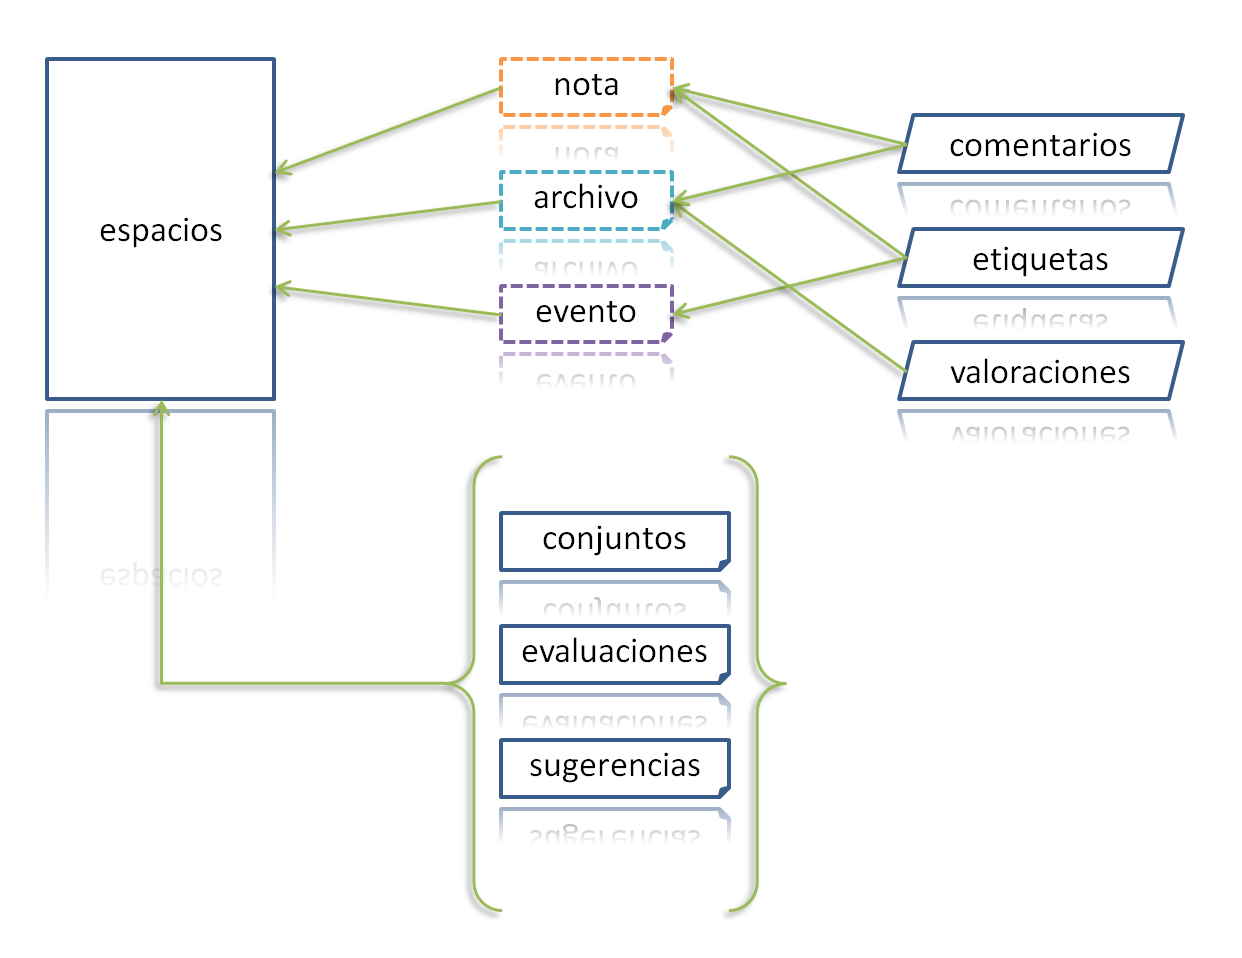
\includegraphics[scale=0.25]{graphics/nomenclatura.png}
 \caption {Relaci\'on entre los conceptos utilizados en el sistema}
 \label {nomenclatura}
\end{figure}

\subsection{Resultados}
Definidos los terminos a utilizarse, a continuaci\'on se present\'an los resultados generados:

\subsubsection{Contexto}
\begin{center}
\begin{tabular}{|l|l|}
\hline
Sitio web & \url{yachay.memi.umss.edu.bo} \\
Periodo acad\'emico & I/2011 \\
Tiempo de evaluaci\'on: & 325 dias. \\
Fecha de inicio: & 23 de Septiembre del 2010. \\
Fecha de fin: & 14 de Agosto del 2011. \\
Lugar de evaluaci\'on: & Carrera de Inform\'atica y Sistemas (UMSS). \\
Ca\'idas del servidor: & 4. \\
Tiempo del servidor fuera de linea: & 2 semanas acumuladas. \\
Docentes participantes: & 4. \\
Materias participantes: & 4. \\
Grupos participantes: & 8. \\
Usuarios participantes: & 542 (estudiantes de primeros semestres). \\
Espacios virtuales creados: & 33. \\
Recursos publicados: & 68. \\
\hline
\end{tabular}
\end{center}
\subsubsection{Usuarios}

En t\'erminos de uso, puede apreciarse en la Figura \ref{usuarios_tabla_1} las diferentes formas de comportamiento de los 
usuarios, seg\'un el rol que desempe\~nan en el sistema.
Destaca en esta tabla la disparidad entre el rol de estudiante y los dem\'as roles, como puede verse en la Figura 
\ref{usuarios_bars_1}, del conjunto de usuarios registrados, \'unicamente el 20\% ingreso alguna vez al sistema,
Es de rescatar adem\'as, que los usuarios fueron registrados autom\'aticamente por sus respectivos docentes.

\begin{figure}[H]
\centering
 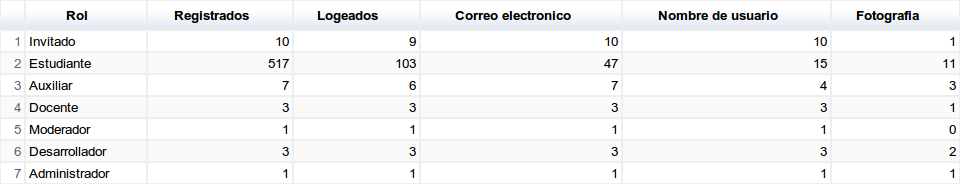
\includegraphics[scale=0.4]{graphics/usuarios_tabla_1.png}
 \caption {Intenci\'on de los usuarios clasificados por rol}
 \label {usuarios_tabla_1}
\end{figure}

\begin{figure}[H]
\centering
 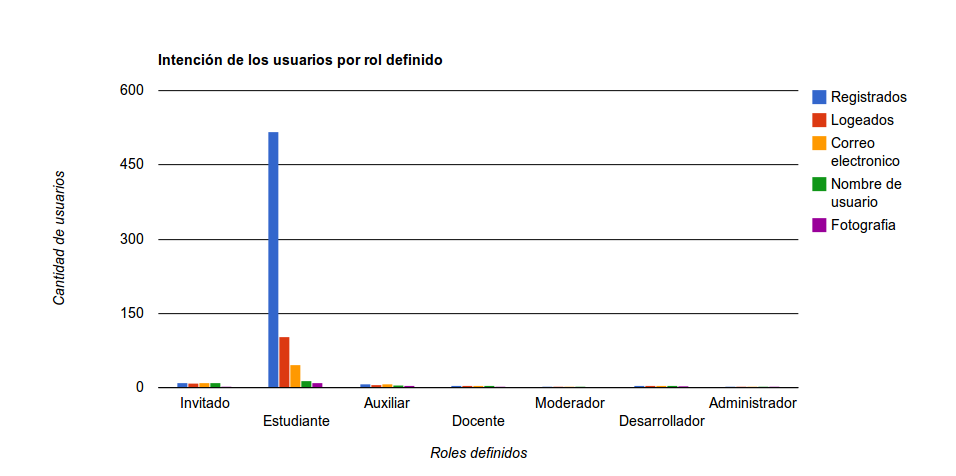
\includegraphics[scale=0.4]{graphics/usuarios_bars_1.png}
 \caption {Diagrama de barras de la intenci\'on de los usuarios clasificados por rol}
 \label {usuarios_bars_1}
\end{figure}

Puede verse en la Figura \ref{usuarios_pie_1} como el predominio en cantidad de los estudiantes va decayendo progresivamente
en intenci\'on frente a los otros roles. Considerando los escasa cantidad de atractivos que posee el sistema es importante 
considerar una audiencia de 126 personas como el primer paso hacia la construcci\'on de un lugar com\'un para el estudio 
realizado.\\

Respecto a la actividad de los usuarios sobre el sistema, puede verse en la Figura \ref{usuarios_tabla_2} la escasisima 
actividad, participaci\'on y popularidad en todos los roles, exceptuando el de los desarrolladores. Puede verse tambi\'en en
la Figura \ref{usuarios_bars_2} el prometedor indicador de sociabilidad, que como puede verse en la Figura 
\ref{usuarios_pie_2} es el mas homog\'eneo, lo que augura una conectividad mas que deseable para los usuarios.

\begin{figure}[H]
\centering
 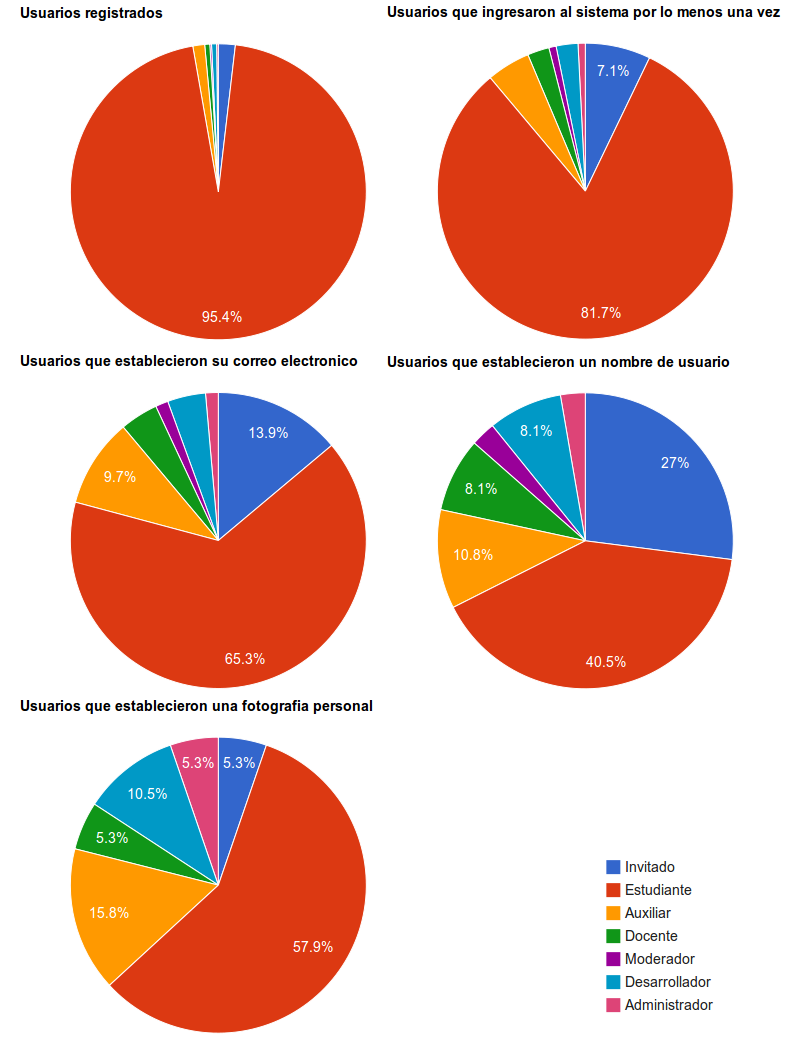
\includegraphics[scale=0.4]{graphics/usuarios_pie_1.png}
 \caption {Porcentajes de intenci\'on de los usuarios clasificados por rol}
 \label{usuarios_pie_1}
\end{figure}

\begin{figure}[H]
\centering
 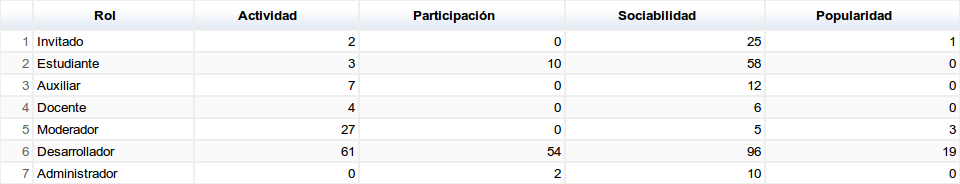
\includegraphics[scale=0.4]{graphics/usuarios_tabla_2.png}
 \caption {Actividad de los usuarios clasificados por rol}
 \label {usuarios_tabla_2}
\end{figure}

\begin{figure}[H]
\centering
 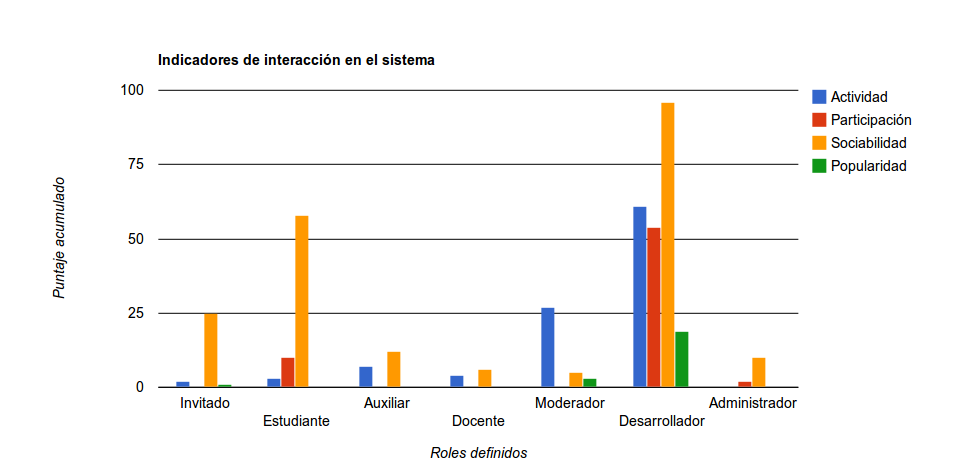
\includegraphics[scale=0.4]{graphics/usuarios_bars_2.png}
 \caption {Diagrama de barras de la actividad de los usuarios clasificados por rol}
 \label {usuarios_bars_2}
\end{figure}

\begin{figure}[H]
\centering
    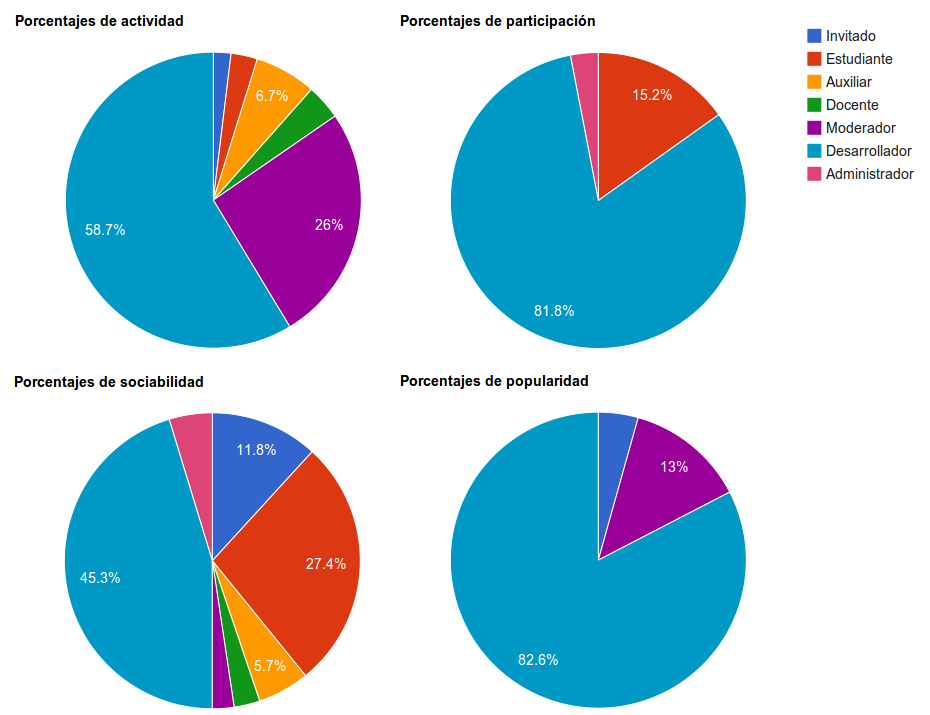
\includegraphics[scale=0.4]{graphics/usuarios_pie_2.png}
    \caption {Porcentajes de actividad clasificados por rol}
    \label {usuarios_pie_2}
\end{figure}

\subsubsection{Contactos}

Considerando los indicadores de sociabilidad, puede apreciarse la matriz de adyacencias (Figura \ref{contactos_matriz}) de la
red social, puede verse que los enlaces fuertes son casi exclusividad propia de los desarrolladores, siendo entre
los otros roles predominantes los enlaces d\'ebiles. Puede verse tambi\'en una sutil relaci\'on entre los usuarios que 
establecieron el nombre de usuario en su perfil, y los niveles de sociabilidad. Cuya interrelaci\'on, es motivo
de seguimiento e intenci\'on de demostraci\'on.
\begin{figure}[H]
\centering
    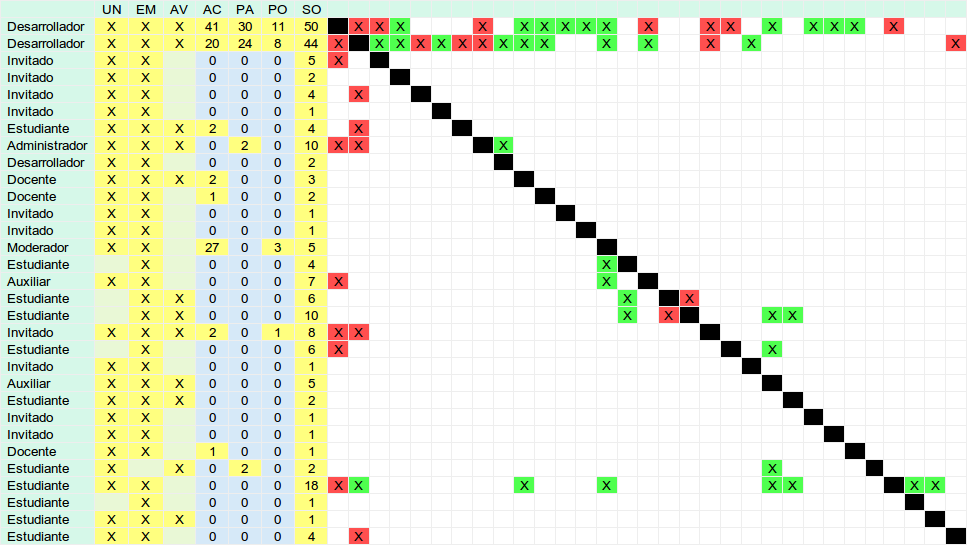
\includegraphics[scale=0.4]{graphics/contactos_matriz.png}
    \caption {Matriz de adyacencia de la red social}
    \label {contactos_matriz}
\end{figure}

\subsubsection{Espacios Virtuales}

En la Figura \ref{espacios_tabla_1} pueden verse los distintos tipos de espacios virtuales y sus indicadores propios, entre 
los que destaca la supremac\'ia del espacio portada, por sobre cualquier otro espacio, siendo el que 
capta mas audiencia de entre los espacios. Tambi\'en es notorio el ausente uso de espacios para equipos de trabajo en los 
grupos, cosa que puede ser debida a las escasez de grupos registrados. Si bien la portada acapara la 
mayor audiencia, no acapara la mayor cantidad de recursos (Figura \ref{espacios_bars_1}), llev\'andose los espacios de 
comunidades un 45\% del contenido del sitio, reforzando la teor\'ia de fomento hacia los espacios menos 
formales (Figura \ref{espacios_pie_1}).
\begin{figure}[H]
\centering
    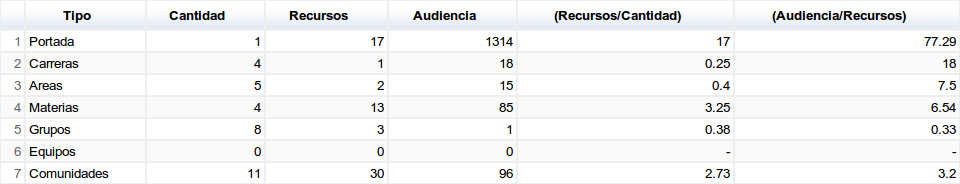
\includegraphics[scale=0.4]{graphics/espacios_tabla_1.png}
    \caption {Clasificaci\'on de los espacios y su actividad}
    \label {espacios_tabla_1}
\end{figure}

\begin{figure}[H]
\centering
    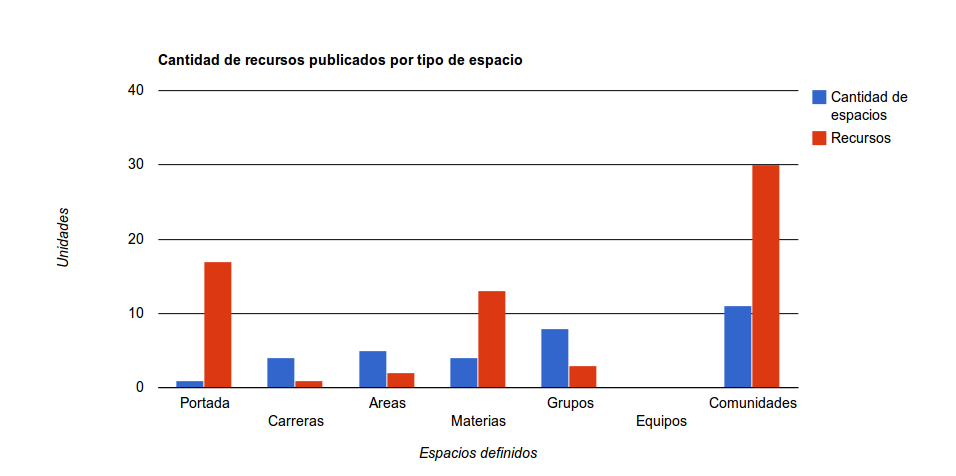
\includegraphics[scale=0.4]{graphics/espacios_bars_1.png}
    \caption {Diagrama de barras de los espacios y sus recursos}
    \label {espacios_bars_1}
\end{figure}

\begin{figure}[H]
\centering
    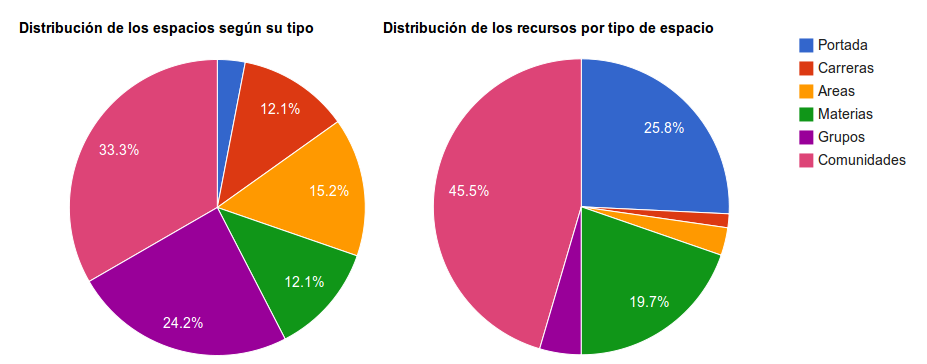
\includegraphics[scale=0.4]{graphics/espacios_pie_1.png}
    \caption {Porcentajes de los espacios y sus recursos seg\'un su tipo}
    \label {espacios_pie_1}
\end{figure}

\subsubsection{Recursos}

Los recursos pueden ser de varios tipos (Figura \ref{recursos_tabla_1}), destacando la gran cantidad de notas 
(Figura \ref{recursos_bars_1}) por sobre los otros tipos de recursos, pudiendo esto deberse a la inmensa facilidad de 
creaci\'on de estas. Aun asi son las fotograf\'ias la que en proporci\'on reciben mejor audiencia, y son los archivos los 
que reciben mayor cantidad de comentarios (Figura \ref{recursos_pie_1}).
\begin{figure}[H]
\centering
    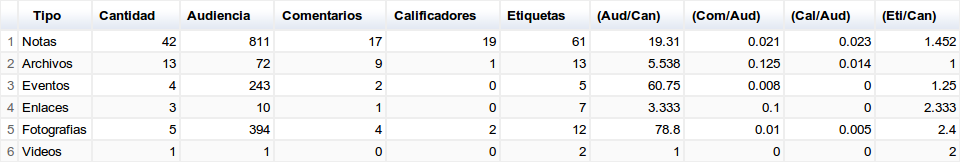
\includegraphics[scale=0.4]{graphics/recursos_tabla_1.png}
    \caption {Clasificaci\'on de los recursos seg\'un su tipo}
    \label {recursos_tabla_1}
\end{figure}

\begin{figure}[H]
\centering
    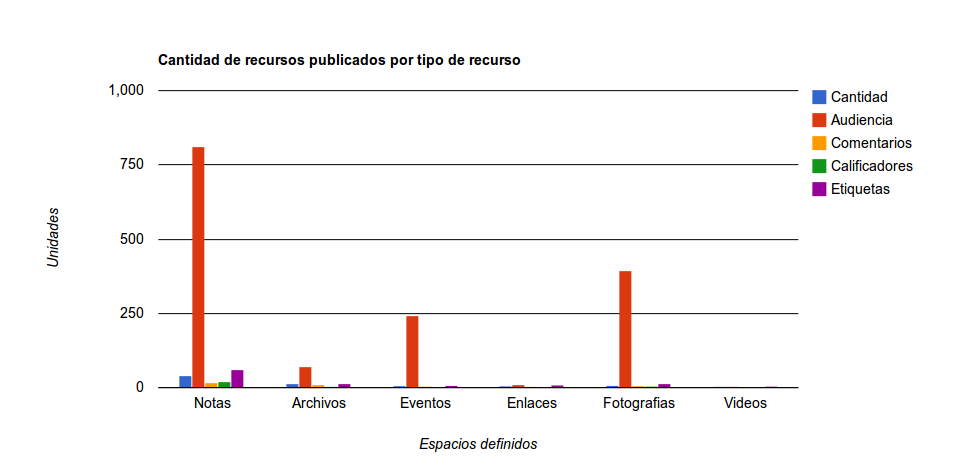
\includegraphics[scale=0.4]{graphics/recursos_bars_1.png}
    \caption {Diagrama de barras de los recursos y sus niveles de repercusi\'on}
    \label {recursos_bars_1}
\end{figure}

\begin{figure}[H]
\centering
    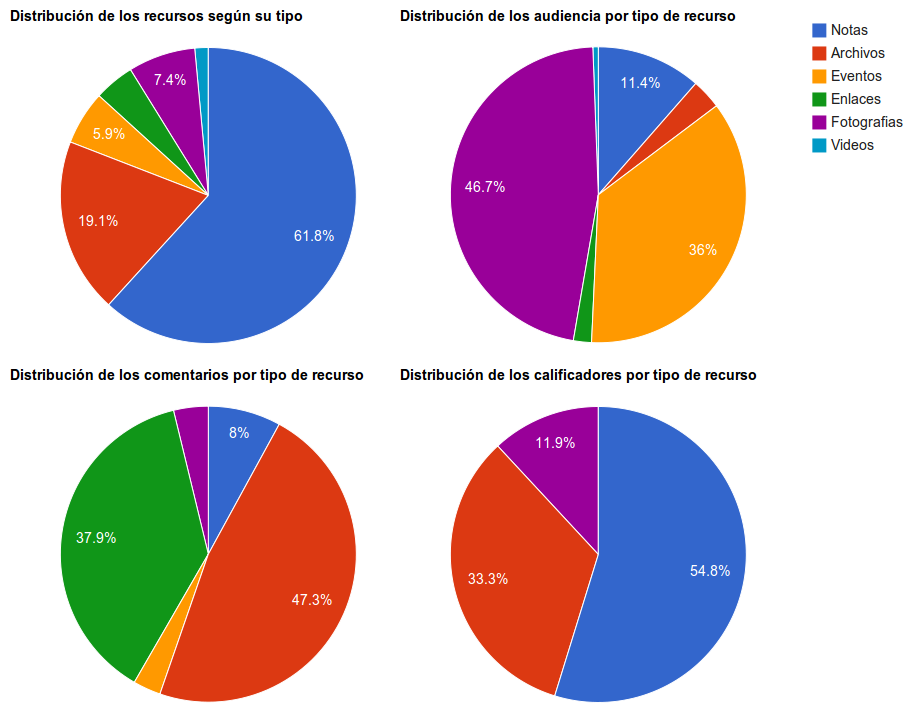
\includegraphics[scale=0.4]{graphics/recursos_pie_1.png}
    \caption {Porcentajes de los recursos seg\'un su tipo}
    \label {recursos_pie_1}
\end{figure}

\subsubsection{Linea de tiempo}

Finalizados los elementos propios de la herramienta, se observan ahora las lineas de tiempo, donde se presentan los tiempos
en los que estos elementos han sido creados.
En la Figura \ref{tiempos_area_1} puede apreciarse en la linea de creaci\'on de los usuarios, los registros autom\'aticos de 
los estudiantes, de parte del docente de su materia, siendo la creaci\'on de usuarios la linea predominante en esta gr\'afica.
\begin{figure}[H]
    \centering
    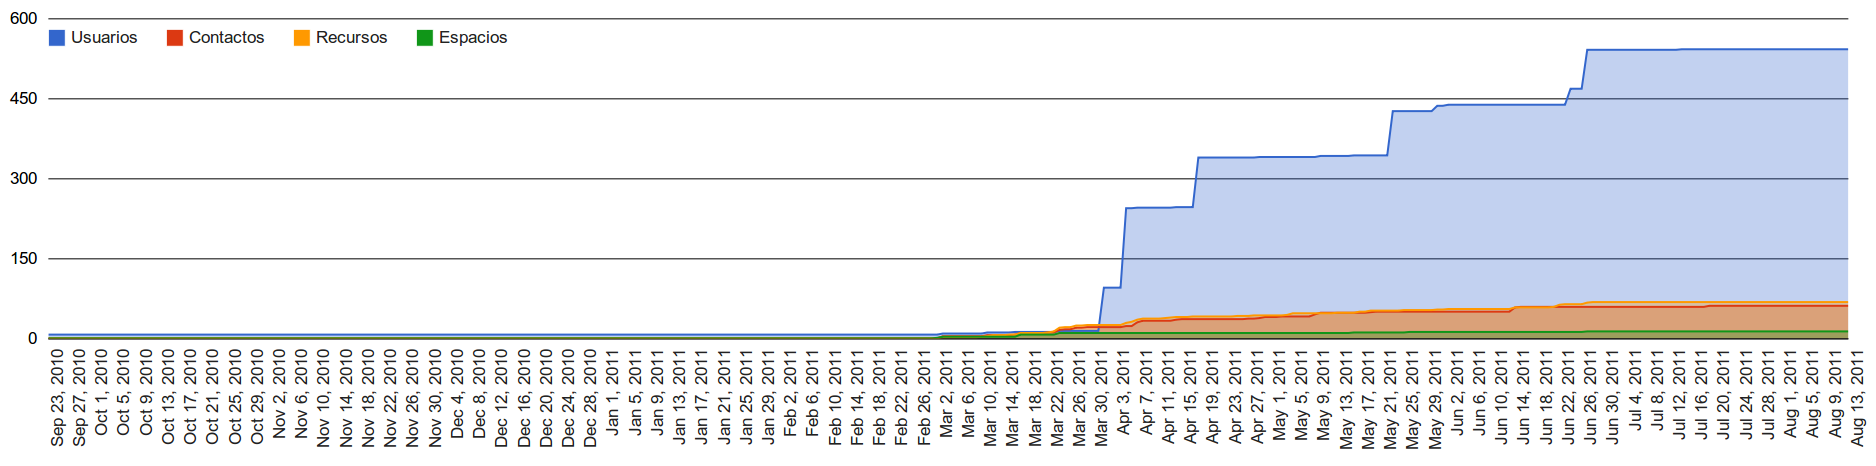
\includegraphics[scale=0.25]{graphics/tiempos_area_1.png}
    \caption {Linea de tiempo de la creaci\'on de elementos en el sistema}
    \label {tiempos_area_1}
\end{figure}

En la Figura \ref{tiempos_area_2} resalta la curiosa relaci\'on entre las lineas de creaci\'on de recursos y la de creaci\'on
de contactos, siendo esta la linea que determina todo el objeto de investigaci\'on.
\begin{figure}[H]
\centering
    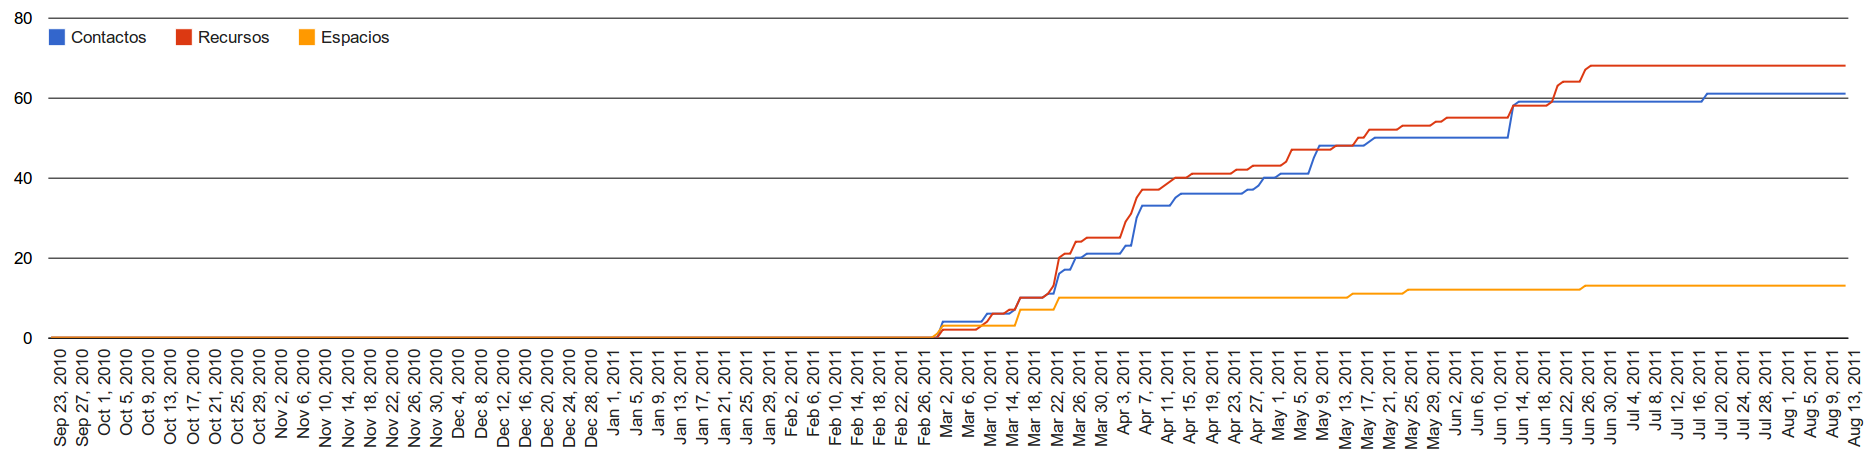
\includegraphics[scale=0.25]{graphics/tiempos_area_2.png}
    \caption {Linea de tiempo de la creaci\'on de elementos en el sistema}
    \label {tiempos_area_2}
\end{figure}


\chapter{Las personas}

\section{El espacio personal \emph{users}}
\section{El control de las funciones \emph{roles}}

\chapter{La red de contactos}

\section{Las redes sociales \emph{contacts}}
\section{Los círculos \emph{sets}}
\section{La propagación \emph{invitations}}

\chapter{Los espacios virtuales}

\section{El espacio genérico \emph{spaces}}
\section{Los espacios formales \emph{gestions}, \emph{careers}, \emph{areas}}
\section{El espacio informal \emph{communities}}
\section{Los espacios jerárquicos \emph{subjects}, \emph{groups}, \emph{teams}}
\section{Las utilidades sobre grupos \emph{groupsets}}
\chapter{El B-learning}

\section{Los sistemas de evaluación \emph{evaluations}}
\section{Las calificaciones \emph{califications}}
%\section{El trabajo para casa \emph{tasks}}

\chapter{Los recursos}

\section{Los componentes genericos \emph{resources}}
\section{El recurso mas basico \emph{notes}}
\section{Los archivos en general \emph{files}}
\section{Los archivos especiales \emph{photos}, \emph{videos}}
\section{Los recursos espacio-temporales \emph{events}}
\section{La reenderizacion personalizada \emph{links}}
\section{Las sugerencias \emph{feedback}}

\chapter{Los aspectos 2.0}

\section{Los comentarios \emph{comments}}
\section{La calidad del recurso \emph{ratings}}
\section{Las nuevas interpretaciones \emph{tags}}
\section{Los sistemas de reputación \emph{valorations}}
\section{Los refuerzos positivos \emph{awards}}

\chapter{Los sistemas de control}

\section{Los indicadores medibles \emph{stats}}
\section{El panel de control \emph{panels}}


\backmatter
\begin{thebibliography}{99}

\bibitem{Jeria} Jeria Carvajal, Esther.\\
\emph{Fenómeno Facebook.}\\
Extraído el 01 de Mayo del 2011, de\\
http://www.bibliodigital.udec.cl/index.php?option=com\_content\
\&task=view\&id=113\&Itemid=9

\bibitem{Rodriguez} Rodríguez Morales, Germania (2008, Mayo).\\
\emph{Educación Superior en Latinoamérica y la Web2.0.}\\
Extraído el 24 de Abril del 2011, de\\
http://www.utpl.edu.ec/gcblog/wp-content/uploads/web2-y-educacion-superior.pdf

\bibitem{Gonzalez} González Mariño, Julio Cesar (2006, Enero).\\
\emph{B-Learning utilizando software libre, una alternativa viable en
Educación Superior.}\\
Universidad Autónoma de Tamaulipas, México.\\
Extraído el 24 de Abril del 2011, de\\
http://revistas.ucm.es/edu/11302496/articulos/RCED0606120121A.PDF

\bibitem{Bartolome} Bartolomé, Antonio (2004).\\
\emph{Blended Learning. Conceptos básicos.}\\
Píxel-Bit. Revista de Medios y Educación, 23, pp. 7-20.\\
Universidad de Barcelona, España.\\
Extraído el 24 de Abril del 2011, de\\
http://www.lmi.ub.es/personal/bartolome/articuloshtml/\\
04\_blended\_learning/documentacion/1\_bartolome.pdf

\bibitem{Santamaria} Santamaria, Fernando.\\
\emph{Algunos apuntes sobre insignias o badges en educación.}\\
Extraído el 24 de Abril del 2011, de\\
http://fernandosantamaria.com/blog/2011/12/\\
algunos-apuntes-sobre-insignias-o-badges-en-educacion/

\bibitem{Rojas} Rojas Velásquez, Freddy (2001, Junio).\\
\emph{Enfoques sobre el aprendizaje humano.}\\
Departamento de Ciencia y Tecnología del Comportamiento.\\
Universidad Simón Bolívar.\\
Extraído el 28 de Septiembre del 2013, de\\
http://ares.unimet.edu.ve/programacion/psfase3/modII/biblio/\\
Enfoques\_sobre\_el\_aprendizaje1.pdf

\bibitem{ABC} Definición ABC.\\
\emph{Definición de conductismo.}\\
Extraído el 30 de Septiembre del 2013, de\\
http://www.definicionabc.com/general/conductismo.php\#ixzz2gQeKv5i6

\bibitem{Glez} Glez Guadarrama, Gerardo.\\
\emph{Repertorios básicos.}\\
Extraído el 30 de Septiembre del 2013, de\\
http://glosarioconductual.blogspot.com/2013/06/repertorios-basicos.html

\bibitem{Venegas} Cuco de Venegas.\\
\emph{Gamificación y SocialCRM.}\\
Extraído el 02 de Octubre del 2013, de\\
http://scrm.waplus.net/?p=44

\bibitem{LasIndias} Indianopedia.\\
\emph{Cultura de la adhesión.}\\
Extraído el 02 de Abril del 2014, de\\
http://lasindias.com/indianopedia/cultura-de-la-adhesion

\bibitem{Santamaria2} Santamaria, Fernando.\\
\emph{Las redes sociales en el ámbito educativo.}\\
Extraído el 03 de Abril del 2014, de\\
http://www.slideshare.net/lernys/las-redes-sociales-en-el-mbito-educativo

\bibitem{Ontalba} Ontalba-Ruipérez, José-Antonio.\\
\emph{Evolución de técnicas de web social en programas educativos: aplicación a
un máster 2.0.}\\
Extraído el 04 de Octubre del 2014, de\\
http://bid.ub.edu/21/ontal2.htm

\bibitem{Silva} Silva Matiz, David Alejandro.\\
\emph{Teoría de Indicadores de Gestión y su Aplicación Práctica.}\\
Extraído el 04 de Octubre del 2014, de\\
http://www.umng.edu.co/documents/10162/745281/V3N2\_29.pdf

\bibitem{Cockburn} Alistair Cockburn 2008.\\
\emph{Using both incremental and iterative development.}\\
Extraído el 04 de Octubre del 2014, de\\
http://alistair.cockburn.us/Using+both+incremental+and+iterative+development

\bibitem{Apache} Apache Foundation.\\
\emph{Apache Virtual Host documentation.}\\
Extraído el 09 de Octubre del 2014, de\\
http://httpd.apache.org/docs/2.0/es/vhosts

\end{thebibliography}


\end{document}
